% !TEX program = xelatex
% 《DSP 指南》中译合订本。章节正文在 chapters/ 下，由 build-tex.sh 从上一级目录的 md 生成。
% 只想看某几章时，把 \includeonly 那行的注释去掉并填上章节号，编译会快很多。
\documentclass[a4paper,zihao=-4,fontset=mac,openany]{ctexbook}

% ---------- 版面 ----------
\usepackage[top=2.5cm,bottom=2.5cm,left=2.6cm,right=2.6cm,headheight=15pt]{geometry}
\linespread{1.35}
\setlength{\parskip}{0.3em}
\setcounter{secnumdepth}{0} % 只给章编号，节保持原书的不编号写法
\setcounter{tocdepth}{1}    % 目录列到节
\ctexset{
  chapter = {number = \arabic{chapter}, format = \huge\bfseries\centering, beforeskip = 10pt, afterskip = 30pt},
  section = {format = \Large\bfseries},
}

% ---------- 字体 ----------
% STIX Two 自带希腊字母和常用符号，正文里的 µ、σ、−、≈ 不会缺字
\usepackage{unicode-math}
\setmainfont{STIX Two Text}
\setmathfont{STIX Two Math}
\setmonofont{Menlo}[Scale=0.85]
% 正文字体缺箭头和部分数学符号，xelatex 不会自动换字体补字；
% md2tex.lua 把正文里的这些字符包成 \dspsym{→}，用 STIX Two Math 显示
\newfontfamily\dspsymfont{STIX Two Math}
\newcommand{\dspsym}[1]{{\dspsymfont #1}}

% ---------- 常用宏包 ----------
\usepackage{amsmath}
\usepackage{graphicx}
\graphicspath{{../}} % md 里的图片路径是 assets/...，相对上一级目录
\usepackage[font=small,labelformat=empty]{caption}
\usepackage{longtable,booktabs,array,calc}
\newcounter{none} % pandoc 生成的无标题表格用 \begin{longtable}[]，需要这个计数器
\usepackage{xcolor}
\usepackage{fvextra}
\fvset{breaklines=true,breakanywhere=true,fontsize=\small}
\usepackage{enumitem}
\setlist{itemsep=0.2em,topsep=0.4em}
\providecommand{\tightlist}{\setlength{\itemsep}{0pt}\setlength{\parskip}{0pt}}

% 代码块浅灰底色、引用块左侧竖线；framed 能跨页断开，且 TeX Live basic 自带
\usepackage{framed}
\definecolor{shadecolor}{gray}{0.95}
% pandoc 代码高亮用到的宏（从 pandoc 默认模板复制，配色为 pygments）
\newcommand{\VerbBar}{|}
\newcommand{\VERB}{\Verb[commandchars=\\\{\}]}
\DefineVerbatimEnvironment{Highlighting}{Verbatim}{commandchars=\\\{\}}
% Add ',fontsize=\small' for more characters per line
\newenvironment{Shaded}{}{}
\newcommand{\AlertTok}[1]{\textcolor[rgb]{1.00,0.00,0.00}{\textbf{#1}}}
\newcommand{\AnnotationTok}[1]{\textcolor[rgb]{0.38,0.63,0.69}{\textbf{\textit{#1}}}}
\newcommand{\AttributeTok}[1]{\textcolor[rgb]{0.49,0.56,0.16}{#1}}
\newcommand{\BaseNTok}[1]{\textcolor[rgb]{0.25,0.63,0.44}{#1}}
\newcommand{\BuiltInTok}[1]{\textcolor[rgb]{0.00,0.50,0.00}{#1}}
\newcommand{\CharTok}[1]{\textcolor[rgb]{0.25,0.44,0.63}{#1}}
\newcommand{\CommentTok}[1]{\textcolor[rgb]{0.38,0.63,0.69}{\textit{#1}}}
\newcommand{\CommentVarTok}[1]{\textcolor[rgb]{0.38,0.63,0.69}{\textbf{\textit{#1}}}}
\newcommand{\ConstantTok}[1]{\textcolor[rgb]{0.53,0.00,0.00}{#1}}
\newcommand{\ControlFlowTok}[1]{\textcolor[rgb]{0.00,0.44,0.13}{\textbf{#1}}}
\newcommand{\DataTypeTok}[1]{\textcolor[rgb]{0.56,0.13,0.00}{#1}}
\newcommand{\DecValTok}[1]{\textcolor[rgb]{0.25,0.63,0.44}{#1}}
\newcommand{\DocumentationTok}[1]{\textcolor[rgb]{0.73,0.13,0.13}{\textit{#1}}}
\newcommand{\ErrorTok}[1]{\textcolor[rgb]{1.00,0.00,0.00}{\textbf{#1}}}
\newcommand{\ExtensionTok}[1]{#1}
\newcommand{\FloatTok}[1]{\textcolor[rgb]{0.25,0.63,0.44}{#1}}
\newcommand{\FunctionTok}[1]{\textcolor[rgb]{0.02,0.16,0.49}{#1}}
\newcommand{\ImportTok}[1]{\textcolor[rgb]{0.00,0.50,0.00}{\textbf{#1}}}
\newcommand{\InformationTok}[1]{\textcolor[rgb]{0.38,0.63,0.69}{\textbf{\textit{#1}}}}
\newcommand{\KeywordTok}[1]{\textcolor[rgb]{0.00,0.44,0.13}{\textbf{#1}}}
\newcommand{\NormalTok}[1]{#1}
\newcommand{\OperatorTok}[1]{\textcolor[rgb]{0.40,0.40,0.40}{#1}}
\newcommand{\OtherTok}[1]{\textcolor[rgb]{0.00,0.44,0.13}{#1}}
\newcommand{\PreprocessorTok}[1]{\textcolor[rgb]{0.74,0.48,0.00}{#1}}
\newcommand{\RegionMarkerTok}[1]{#1}
\newcommand{\SpecialCharTok}[1]{\textcolor[rgb]{0.25,0.44,0.63}{#1}}
\newcommand{\SpecialStringTok}[1]{\textcolor[rgb]{0.73,0.40,0.53}{#1}}
\newcommand{\StringTok}[1]{\textcolor[rgb]{0.25,0.44,0.63}{#1}}
\newcommand{\VariableTok}[1]{\textcolor[rgb]{0.10,0.09,0.49}{#1}}
\newcommand{\VerbatimStringTok}[1]{\textcolor[rgb]{0.25,0.44,0.63}{#1}}
\newcommand{\WarningTok}[1]{\textcolor[rgb]{0.38,0.63,0.69}{\textbf{\textit{#1}}}}

\renewenvironment{Shaded}{\begin{snugshade}}{\end{snugshade}}
\renewenvironment{quote}
  {\def\FrameCommand{{\color{black!30}\vrule width 2pt}\hspace{8pt}}%
   \MakeFramed{\advance\hsize-\width\FrameRestore}\small\color{black!75}}
  {\endMakeFramed}

\usepackage[colorlinks=true,linkcolor=blue!50!black,urlcolor=blue!50!black,bookmarksnumbered]{hyperref}
\usepackage{bookmark}
\usepackage{xurl}

\title{\textbf{数字信号处理：科学家与工程师指南}\\[1em]\Large The Scientist and Engineer's Guide to Digital Signal Processing\\[0.5em]\large（中译本）}
\author{Steven W. Smith 著}
\date{}

% \includeonly{chapters/02,chapters/03}

\begin{document}

\frontmatter
\maketitle
% !TEX root = ../main.tex
% 本文件由 build-tex.sh 从 00b-DSP指南-前言中译.md 生成，改内容请改 md 后重新生成

\chapter{前言}\label{ch-00b}

\section{本书的目标与策略}

技术世界变化得非常快。仅仅 15
年里，个人电脑的性能就提高了将近一千倍。大家普遍认为，接下来 15
年它还会再提高一千倍。这么大的算力改变了科学和工程的做法，数字信号处理(Digital
Signal Processing, DSP)就是最好的例子。

20 世纪 80 年代初，DSP
还是电气工程专业的研究生课程。十年后，它已经成了本科的标准课程。到今天，许多领域的科学家和工程师都要把
DSP 当成一项基本技能。可惜 DSP 的教学没能及时跟上这个变化。几乎所有 DSP
教材仍按传统电气工程的写法，堆满了细致而严谨的数学。DSP
的威力大得惊人，但如果你看不懂它，就用不了它！

这本书是写给各个领域的科学家和工程师的，比如物理、生物工程、地质、海洋学、机械工程和电气工程等。它的目标是讲清实用的技术，同时绕开繁琐的数学和抽象的理论这两道门槛。为此，写作时用了三条策略：

\textbf{第一，把技术讲明白，而不是只用数学推导证明它成立。}
书里仍保留了不少数学，但数学不是传递信息的主要手段。没有什么比几段写得好的文字配上好的插图更管用。

\textbf{第二，把复数(complex
numbers)当作进阶内容，等基本原理弄懂之后再学。} 第 1～29
章只用代数讲清所有基本技术，极少数地方会用到一点初等微积分。第 30～33
章再讲复数数学怎样扩展 DSP
的能力，介绍那些光靠实数做不到的技术。很多人会觉得这种安排离经叛道！传统
DSP 教材通篇都是复数数学，而且常常从第一章就开始。

\textbf{第三，只用非常简单的计算机程序。} 大多数 DSP 程序用 C、Fortran
或类似的语言编写。但\emph{学} DSP 和\emph{用} DSP
的需求不一样。学生需要把精力集中在算法和技术上，不该被某门语言的怪癖分心。强大和灵活在这里不重要，简单才是关键。书里的程序只为用最直接的方式教
DSP
而写，其他因素都排在后面。只要能让程序逻辑更清楚，好的编程风格也可以不顾。比如：

\begin{itemize}
\tightlist
\item
  使用一种简化版的 BASIC 语言
\item
  带行号
\item
  唯一的控制结构是 FOR-NEXT 循环
\item
  没有输入输出(I/O)语句
\end{itemize}

这是我能找到的最简单的编程风格。有人可能会觉得程序要是用 C
写，这本书会更好。我完全不同意。

\section{目标读者}

这本书主要用作一学年的实用 DSP
课程教材，学生来自各种理工科领域。建议的先修课程有：

\begin{itemize}
\tightlist
\item
  一门实用电子学课程（运算放大器(op amp)、RC 电路等）
\item
  一门计算机编程课程（Fortran 或类似语言）
\item
  一年的微积分
\end{itemize}

写这本书时也考虑到了在职的专业人员。书里讨论了很多日常的 DSP
应用：数字滤波器、神经网络、数据压缩、音频和图像处理等。这些章节尽量各自独立，读者想解决某个具体问题时，不必把整本书重读一遍。

\section{Analog Devices 公司的支持}

本书第二版新增了两章，讲数字信号处理器(Digital Signal
Processors)，也就是专门用来执行 DSP 任务的微处理器。这两章的大部分资料由
Analog Devices 公司（ADI）慷慨提供。ADI
是信号处理电子元器件研发和制造领域的全球领先企业。ADI
的鼓励和支持大大拓宽了本书的范围，也说明了一点：DSP
算法只有配上合适的硬件才能真正派上用场。

\tableofcontents

\mainmatter
% !TEX root = ../main.tex
% 本文件由 build-tex.sh 从 01-DSP指南-第1章中译.md 生成，改内容请改 md 后重新生成

\chapter{DSP 的广度与深度}\label{ch-01}

数字信号处理(Digital Signal Processing, DSP)是塑造 21
世纪科学与工程的最强大的技术之一。它已经在许多领域带来了革命性的变化，比如通信、医学成像、雷达与声呐、高保真音乐重放、石油勘探等。每个领域都发展出了深厚的
DSP
技术，有自己的算法、数学和专门技巧。既广又深，所以任何一个人都不可能掌握已有的全部
DSP 技术。学 DSP
要做两件事：一是学整个领域通用的一般概念，二是学你自己感兴趣的那个方向的专门技术。本章先介绍
DSP 在几个截然不同的领域里产生的巨大影响，以此开启我们的 DSP
之旅。革命已经开始了。

\section{DSP 的起源}

数字信号处理和计算机科学其他分支的区别，在于它处理的数据类型很特别：信号(signals)。大多数情况下，这些信号最初是来自真实世界的感知数据，比如地震的振动、视觉图像、声波等。DSP
就是在这些信号被转换成数字形式之后，用来加工它们的数学、算法和技术。它的目标五花八门，比如：增强视觉图像、识别和生成语音、压缩数据以便存储和传输等。假设我们给计算机接上一个模数转换器(analog-to-digital
converter)，用它采集了一段真实世界的数据。DSP
回答的问题就是：接下来做什么？

DSP 起源于 20 世纪 60～70
年代，那时数字计算机刚刚出现。当时计算机很贵，DSP
只用在少数关键应用上。先驱性的工作集中在四个关键领域：雷达与声呐，关系到国家安全；石油勘探，能赚大钱；太空探索，数据无法重来；医学成像，能救人命。

20 世纪 80～90 年代的个人电脑革命，让 DSP 的新应用呈爆炸式增长。推动 DSP
的不再是军方和政府的需求，一下子变成了商业市场。在这个飞速扩张的领域里，凡是觉得能赚到钱的人，一下子都成了
DSP 供应商。DSP 通过手机、CD
播放机、电子语音信箱这类产品走进了大众生活。图 1-1 展示了其中一些应用。

这场技术革命是自上而下发生的。20 世纪 80 年代初，DSP
还是电气工程专业的研究生课程。十年后，它已经成了本科的标准课程。到今天，许多领域的科学家和工程师都要把
DSP 当成一项基本技能。打个比方，DSP
可以和上一场技术革命------电子学------相比。电子学虽然仍属于电气工程的地盘，但几乎每个科学家和工程师都懂一些基本的电路设计。不懂的话，他们在技术世界里会寸步难行。DSP
的未来也会是这样。

\textbf{图 1-1　DSP
给科学与工程的许多领域带来了革命，这里列出其中一些应用。}

{\def\LTcaptype{none} % do not increment counter
\begin{longtable}[]{@{}ll@{}}
\toprule\noalign{}
领域 & 应用 \\
\midrule\noalign{}
\endhead
\bottomrule\noalign{}
\endlastfoot
太空 & 太空照片增强；数据压缩；远程太空探测器的智能感知分析 \\
医疗 & 诊断成像（CT、MRI、超声等）；心电图分析；医学图像的存储与检索 \\
商业 & 多媒体展示用的图像和声音压缩；电影特效；视频会议 \\
电话 & 语音和数据压缩；回声抑制；信号复用；滤波 \\
军事 & 雷达；声呐；武器制导；保密通信 \\
工业 & 石油和矿产勘探；生产过程监测与控制；无损检测；CAD 与设计工具 \\
科研 & 地震记录与分析；数据采集；频谱分析；仿真与建模 \\
\end{longtable}
}

这段近代史不只是一个趣闻，它会极大地影响你学习和使用 DSP
的能力。假设你遇到一个 DSP
问题，去教材或其他文献里找答案。你通常会看到一页接一页的方程、晦涩的数学符号和陌生的术语。简直是噩梦！很多
DSP
文献连这个领域的老手都看得一头雾水。这并不是说这些材料有什么问题，只是它们是写给非常专业的读者看的。走在最前沿的研究者需要这种细致的数学，才能理解工作在理论上的含义。

本书的一个基本前提是：大多数实用的 DSP
技术，不必跨过繁琐数学和理论这道传统门槛，也能学会、能用好。《科学家与工程师的数字信号处理指南》是写给想把
DSP 当成工具，而不是当成新职业的人。

本章剩下的部分会介绍 DSP
带来革命性变化的那些领域。读每个应用时请留意：DSP
是高度跨学科的，要依靠许多相邻领域的技术成果。如图 1-2 所示，DSP
和其他技术学科之间的边界并不清晰分明，而是模糊、互相重叠的。如果你想专攻
DSP，这些相关领域也都要学。

\textbf{图
1-2　数字信号处理与科学、工程、数学的许多其他领域边界模糊、互相重叠。}

\begin{quote}
图中围绕「数字信号处理」的相邻领域有：通信理论(Communication
Theory)、数值分析(Numerical Analysis)、概率与统计(Probability and
Statistics)、模拟信号处理(Analog Signal Processing)、决策理论(Decision
Theory)、模拟电子学(Analog Electronics)、数字电子学(Digital
Electronics)。
\end{quote}

\section{电信}

电信(Telecommunications)就是把信息从一个地方传到另一个地方。信息的形式有很多：电话通话、电视信号、计算机文件以及其他各种数据。要传信息，两地之间就需要一条信道(channel)，可以是一对导线、无线电信号、光纤等。电信公司靠帮客户传信息收钱，同时又要花钱建设和维护信道。账算起来很简单：一条信道里能传的信息越多，赚的钱就越多。DSP
在电信业的许多方面带来了革命：信令音的生成与检测、频带搬移、滤除电源线的嗡嗡声等。这里讨论电话网络中的三个具体例子：复用、压缩和回声控制。

\subsection{复用}

全世界大约有十亿部电话。只要按几个键，交换网络就能在几秒钟内把其中任意一部和另一部接通。这项任务的规模大得惊人！直到
20 世纪 60
年代，两部电话之间的连接还需要让模拟语音信号经过机械开关和放大器，一路通话就要占一对导线。相比之下，DSP
把音频信号转换成一串串行的数字数据。比特很容易交织在一起、之后再拆开，所以一条信道上可以同时传很多路电话。例如，有一种叫
T 载波系统(T-carrier system)的电话标准，能同时传 24 路语音。每路语音用 8
比特的压扩(companded，即对数压缩)模数转换，每秒采样 8000
次。这样每路语音用 64,000 比特/秒表示，24 路合在一起是 1.544
兆比特/秒。用普通的 22 号铜线电话线，这个信号能传约 6000
英尺，这是典型的互连距离。数字传输的经济优势巨大：导线和模拟开关很贵，数字逻辑门很便宜。

\subsection{压缩}

语音信号以每秒 8000
个采样数字化后，大部分数字信息是冗余的。也就是说，任何一个采样携带的信息，大部分都和相邻采样重复。人们已经开发了几十种
DSP
算法，把数字化的语音信号转换成每秒所需比特更少的数据流，这些叫数据压缩(data
compression)算法。再用与之配套的解压算法把信号还原成原来的样子。这些算法的压缩程度和压缩后的音质各不相同。一般来说，把数据率从
64 千比特/秒降到 32 千比特/秒，音质不会有损失。压到 8
千比特/秒时，声音会明显受影响，但用于长途电话网仍然够用。能达到的最高压缩大约是
2 千比特/秒，这时声音失真很严重，但在军事和水下通信等某些场合仍然可用。

\subsection{回声控制}

回声是长途电话连接中的一个严重问题。你对着电话说话时，代表你声音的信号传到对方的接收端，其中一部分会作为回声返回来。如果连接距离在几百英里以内，收到回声的延迟只有几毫秒。人耳习惯听到这种短延迟的回声，通话听起来很正常。距离越远，回声就越明显、越恼人。洲际通信的延迟可能达到几百毫秒，特别让人难受。数字信号处理解决这类问题的办法是：测量返回的信号，生成一个合适的反信号(antisignal)，把讨厌的回声抵消掉。同样的技术让免提电话的用户能同时听和说，而不会和音频反馈（啸叫）较劲。它还能用来降低环境噪声，办法是用数字生成的反噪声(antinoise)把噪声抵消掉。

\section{音频处理}

人类最主要的两种感官是视觉和听觉。相应地，DSP
的很大一部分都和图像处理、音频处理有关。人们既听音乐也听语音，DSP
在这两方面都带来了革命性的变化。

\subsection{音乐}

从乐手的麦克风到发烧友的音箱，这条路出奇地长。用数字形式表示数据很重要，可以避免模拟存储和处理通常带来的劣化。比较过磁带和
CD
音质的人对此都很熟悉。典型的流程是：一首乐曲在录音棚里分多个声道或音轨录制，有时甚至把每件乐器和每位歌手分开录。这样做是为了让录音师在制作最终成品时有更大的灵活性。把各条音轨合成最终成品的复杂过程叫缩混(mix
down)。缩混时 DSP
能提供几项重要功能，包括：滤波、信号相加相减、信号剪辑等。

在音乐制作中，最有意思的 DSP 应用之一是人工混响(artificial
reverberation)。如果只是把各个声道简单地加在一起，得到的音乐听起来单薄、寡淡，就像乐手在室外演奏一样。这是因为听众受音乐中回声或混响成分的影响很大，而录音棚通常会把这些成分压到最低。DSP
可以在缩混时加入人工回声和混响，模拟各种理想的聆听环境。延迟几百毫秒的回声给人身处大教堂的感觉；延迟
10～20 毫秒的回声则让人感觉在一个大小适中的房间里。

\subsection{语音生成}

语音生成和语音识别用于人与机器之间的交流。你不用手和眼，而是用嘴和耳。当你的手和眼该做别的事时，这就非常方便，比如开车、做手术，或者（很遗憾地）向敌人开火。计算机生成语音有两种方法：数字录音和声道模拟(vocal
tract
simulation)。数字录音是把真人说话的声音数字化后存起来，通常以压缩形式存储。播放时把存储的数据解压，再转换回模拟信号。整整一小时的录音只需约
3
兆字节的存储空间，连小型计算机系统都完全能应付。这是如今最常用的数字语音生成方法。

声道模拟器更复杂，它试图模仿人类发声的物理机制。人的声道是一个声学腔体，它的共振频率由各个腔室的大小和形状决定。声道里的声音有两种基本来源，叫浊音(voiced
sounds)和擦音(fricative
sounds)。浊音是声带振动，向声腔送出近似周期性的气流脉冲。擦音则来自气流在狭窄处（如牙齿和嘴唇）形成的嘈杂湍流。声道模拟器先生成类似这两种激励的数字信号，再让激励信号通过一个具有类似共振的数字滤波器，以此模拟共振腔的特性。DSP
最早的成功案例之一就用了这种方法：Speak \&
Spell，一款畅销的儿童电子学习机。

\subsection{语音识别}

自动识别人类语音比生成语音难得多。语音识别是「人脑擅长、数字计算机却很不擅长」的经典例子。数字计算机能存储和调取海量数据，以惊人的速度做数学计算，做重复任务也不会厌烦或懈怠。可惜如今的计算机面对原始的感知数据时表现很差。教计算机每月给你寄电费单很容易，教同一台计算机听懂你的声音却是一项大工程。

数字信号处理处理语音识别问题，一般分两步：先做特征提取(feature
extraction)，再做特征匹配(feature
matching)。先把输入音频里的每个词分离出来，再分析它，确定激励类型和共振频率。然后把这些参数和以前说过的词的样本比较，找出最接近的匹配。这类系统往往只能识别几百个词，只接受词与词之间有明显停顿的语音，而且换一个说话人就得重新训练。这对许多商业应用来说够用了，但和人类听觉的能力相比，这些局限让人汗颜。这个领域还有大量工作要做，谁能做出成功的商业产品，回报会非常丰厚。

\section{回声定位}

想获得远处物体的信息，一种常见的办法是让波打到它身上再反射回来。例如，雷达发射无线电波脉冲，然后检查接收到的信号里有没有飞机反射的回波。声呐在水里发射声波，探测潜艇和其他水下物体。地球物理学家很早就用这种方法探测地下：引爆炸药，再听深埋岩层传回的回声。这些应用虽然原理相通，但各有各的问题和需求。数字信号处理在这三个领域都带来了革命性的变化。

\subsection{雷达}

雷达(Radar)是 RAdio Detection And
Ranging（无线电探测与测距）的缩写。在最简单的雷达系统里，无线电发射机产生一个几微秒长的射频能量脉冲。这个脉冲送进一个方向性很强的天线，形成的无线电波以光速向外传播。处在这束波路径上的飞机会把一小部分能量反射回来，被设在发射点附近的接收天线收到。物体的距离由发射脉冲和收到回波之间的时间差算出。物体的方向更容易确定：收到回波时你把定向天线指向了哪里，物体就在哪里。

雷达系统的作用距离由两个参数决定：初始脉冲有多少能量，以及无线电接收机的噪声水平。可惜要增加脉冲的能量，通常就得把脉冲加长。而脉冲越长，时间差测量的准确度和精密度就越低。于是两个重要参数之间产生了矛盾：探测远处物体的能力，和准确测定物体距离的能力。

DSP 在三个方面给雷达带来了革命，都和这个基本问题有关。第一，DSP
可以在接收后压缩脉冲，在不减小作用距离的前提下更准确地测距。第二，DSP
可以对接收信号滤波，降低噪声，从而在不损害测距准确度的前提下增大作用距离。第三，DSP
能快速选择和生成不同形状、不同长度的脉冲，这样就能针对特定的探测问题优化脉冲。厉害的地方在于：这些处理很多是在和所用射频相当的采样率下完成的，高达几百兆赫！在雷达领域，DSP
既是算法问题，也同样是高速硬件设计问题。

\subsection{声呐}

声呐(Sonar)是 SOund NAvigation and
Ranging（声音导航与测距）的缩写。它分为主动声呐和被动声呐两类。主动声呐向水中发射
2 kHz～40 kHz
的声脉冲，然后检测并分析回声。主动声呐的用途包括：探测和定位水下物体、导航、通信以及绘制海底地图。典型的最大作用距离是
10～100
公里。被动声呐则只是听水下的声音，包括自然湍流、海洋生物，以及潜艇和水面船只发出的机械声。被动声呐不发出任何能量，所以非常适合隐蔽行动：你想发现对方，又不想被对方发现。被动声呐最重要的应用是探测和跟踪潜艇的军事监视系统。被动声呐通常比主动声呐用更低的频率，因为低频声波在水中传播时被吸收得更少。探测距离可达几千公里。

DSP
给声呐带来革命的方面和雷达大多相同：脉冲生成、脉冲压缩以及对检测信号的滤波。从一方面看，声呐比雷达简单，因为涉及的频率更低。从另一方面看，声呐比雷达难，因为水下环境远没有那么均匀和稳定。声呐系统通常使用庞大的发射和接收阵元阵列，而不只是单个通道。只要恰当地控制和混合这许多阵元的信号，声呐系统就能把发出的脉冲导向想要的位置，并判断回声来自哪个方向。为了处理这么多通道，声呐系统需要和雷达同样庞大的
DSP 计算能力。

\subsection{反射地震学}

早在 20 世纪 20
年代，地球物理学家就发现可以用声音探测地壳结构。勘探人员可以引爆炸药，记录地下十多公里处各个分界层传回的回声。这些回声地震图(seismograms)靠肉眼判读，用来绘制地下结构图。反射地震法(reflection
seismic method)很快成为寻找石油和矿藏的主要方法，至今仍是如此。

理想情况下，送入地下的声脉冲每穿过一个分界层，就产生一个回声。可惜实际情况通常没这么简单。每个返回地面的回声，都必须穿过它产生处上方的所有其他分界层。回声可能在层与层之间来回反弹，于是地面上会检测到「回声的回声」。这些二次回声会让检测到的信号非常复杂，难以判读。从
20 世纪 60
年代起，数字信号处理就被广泛用来在反射地震图中把一次回声和二次回声分开。早期的地球物理学家没有
DSP
是怎么办的？答案很简单：他们只在容易的地方找，也就是多次反射很少的地方。DSP
让人们能在困难的地方找到石油，比如海底。

\section{图像处理}

图像是具有特殊性质的信号。第一，图像测量的是某个参数随空间（距离）的变化，而大多数信号测量的是某个参数随时间的变化。第二，图像包含大量信息。例如，存一秒钟的电视视频可能需要
10
兆字节以上，比同样时长的语音信号多一千多倍。第三，评判图像质量的最终标准往往是人的主观评价，而不是客观指标。这些特殊性质让图像处理成了
DSP 中一个独立的分支。

\subsection{医疗}

1895 年，威廉·康拉德·伦琴(Wilhelm Conrad Röntgen)发现 X
射线能穿透相当厚的物质。能看到活人身体内部，这给医学带来了革命。短短几年里，医用
X 射线系统就遍及全世界。尽管 X 射线成像显然很成功，但在 20 世纪 70 年代
DSP
及相关技术出现之前，它一直受四个问题的限制。第一，体内的结构会互相重叠、互相遮挡。例如，心脏的一部分可能被肋骨挡住看不见。第二，相似的组织不一定分得开。例如，能把骨头和软组织分开，却分不清肿瘤和肝脏。第三，X
射线图像显示的是解剖结构(anatomy，即身体的构造)，而不是生理功能(physiology，即身体的运作)。活人的
X 光片和死人的 X 光片看起来一模一样！第四，X
射线照射会致癌，所以必须谨慎使用，只有在理由充分时才用。

结构重叠的问题在 1971
年得到解决，那年出现了第一台计算机断层扫描仪（以前叫计算机轴向断层扫描仪，CAT
扫描仪）。计算机断层成像(Computed Tomography,
CT)是数字信号处理的一个经典例子。让来自许多方向的 X
射线穿过病人身体被检查的部位。不是直接用检测到的 X
射线成像，而是把信号转换成数字数据存进计算机，再用这些信息计算出看起来像身体切片的图像。这些图像比传统技术显示的细节多得多，大大改进了诊断和治疗。CT
的影响几乎和当初 X
射线成像问世一样大。短短几年里，世界上每家大医院都用上了 CT 扫描仪。1979
年，CT 的两位主要贡献者戈弗雷·亨斯菲尔德(Godfrey N.
Hounsfield)和艾伦·科马克(Allan M. Cormack)分享了诺贝尔医学奖。这才叫好的
DSP！

X 射线的后三个问题，是靠改用 X
射线以外的穿透性能量（如无线电波和声波）解决的。DSP
在所有这些技术中都起着关键作用。例如，磁共振成像(Magnetic Resonance
Imaging,
MRI)把磁场和无线电波结合起来探查人体内部。恰当地调节磁场的强度和频率，会让身体某个局部区域的原子核在量子能态之间共振。这种共振会发出二次无线电波，被放在身体附近的天线检测到。检测到的信号的强度和其他特征，提供了这个共振区域的信息。调节磁场可以让共振区域扫过全身，从而绘出内部结构。这些信息通常和
CT 一样以图像形式呈现。MRI
除了能很好地区分不同类型的软组织，还能提供生理功能的信息，比如动脉中的血流。MRI
完全依赖数字信号处理技术，没有它就无法实现。

\subsection{太空}

有时候，你只能从一张糟糕的照片里尽量榨出信息。无人卫星和太空探测器拍的图像经常就是这样。没人会为了拧一下相机的旋钮专门派个修理工去火星！DSP
可以从几个方面改善在极端不利条件下拍摄的图像质量：亮度和对比度调整、边缘检测(edge
detection)、降噪、对焦调整、运动模糊消除等。有空间畸变的图像，比如给球形行星拍平面照片时遇到的那种，也可以通过变形(warp)校正成正确的样子。还可以把许多张单独的图像合并成一个数据库，用独特的方式展示信息，例如生成一段模拟在遥远行星表面上空飞行的视频。

\subsection{商业成像产品}

对于大量卖给普通大众的系统来说，图像信息量大是个问题。商业系统必须便宜，而这和大容量内存、高数据传输率很难兼顾。解决这个两难的一个办法是图像压缩。和语音信号一样，图像里含有大量冗余信息，可以用算法减少表示图像所需的比特数。电视和其他活动图像特别适合压缩，因为相邻帧之间图像的大部分内容保持不变。利用这项技术的商业成像产品包括：可视电话、播放活动图像的计算机程序以及数字电视。

% !TEX root = ../main.tex
% 本文件由 build-tex.sh 从 02-DSP指南-第2章中译.md 生成，改内容请改 md 后重新生成

\chapter{统计、概率与噪声}\label{ch-02}

在数字信号处理里，统计(statistics)和概率(probability)用来刻画信号以及产生信号的过程。例如，DSP
的一个主要用途是减少采集数据中的干扰、噪声(noise)和其他不想要的成分。这些成分可能是被测信号本身固有的，可能来自数据采集系统的缺陷，也可能是某种
DSP
操作不可避免的副产品。统计和概率能把这些干扰特征测出来、分好类，这是制定去除策略的第一步。本章介绍统计和概率中最重要的概念，重点放在它们怎样应用于采集到的信号。

\section{信号与图表的术语}

信号(signal)描述的是一个参数和另一个参数之间的关系。例如，模拟电子学中最常见的信号是随时间变化的电压。两个参数都能取连续范围内的值，所以我们称之为连续信号(continuous
signal)。相比之下，把这个信号送进模数转换器，两个参数都会被强制量化(quantized)。比如，设想用
12 比特、每秒 1000 个采样的速率来转换。电压被限定在
4096（\(2^{12}\)）个可能的二进制电平上，时间也只在每隔一毫秒的时刻上有定义。由这样量化后的参数构成的信号，称为离散信号(discrete
signal)或数字化信号(digitized
signal)。大体上说，连续信号存在于自然界，离散信号存在于计算机内部（两边都能找到例外）。也有一个参数连续、另一个参数离散的信号。这种混合信号很少见，没有专门的名字，用到时必须明确说明两个参数各自的性质。

图 2-1
展示了两个离散信号，就像用数字数据采集系统采到的那样。纵轴可以表示电压、光强、声压，或者无数种其他参数。这里我们不知道它具体代表什么，所以给它一个通用标签：幅度(amplitude)。这个参数还有好几个别名：y
轴、因变量(dependent variable)、值域(range)、纵坐标(ordinate)。

横轴表示信号的另一个参数，它的名字有：x 轴、自变量(independent
variable)、定义域(domain)、横坐标(abscissa)。采集到的信号，横轴上最常见的参数是时间；不过在特定应用里也会用其他参数。例如，地球物理学家可能沿地表每隔相等距离测一次岩石密度。为了保持通用，我们把横轴简单地标为：采样序号(sample
number)。如果是连续信号，就得换别的标签，比如时间、距离、x 等。

构成信号的两个参数一般不能互换。y 轴上的参数（因变量）被称为 x
轴上参数（自变量）的函数。换句话说，自变量描述每个采样是怎样、在什么时候取的，因变量才是实际的测量值。给定
x 轴上的一个值，总能找到 y 轴上对应的值，但反过来通常不行。

要特别留意「域(domain)」这个词，它在 DSP
里用得非常广。例如，以时间为自变量（即横轴参数）的信号，称为处在时域(time
domain)。DSP 里另一种常见信号以频率为自变量，于是有了频域(frequency
domain)这个词。同样，以距离为自变量的信号称为处在空间域(spatial
domain)（距离是对空间的度量）。横轴上是什么参数，信号就处在什么域，就这么简单。如果
x
轴标的是很笼统的东西，比如「采样序号」呢？作者们通常说这类信号处在时域。因为按相等时间间隔采样是获取信号最常见的方式，而且也没有更具体的叫法。

图 2-1
中的信号虽然是离散的，却画成了连续的线。这是因为采样点太多，如果一个个画成标记点就分不清了。在描绘较短信号的图里，比如少于
100
个采样，通常会画出每个标记点。至于要不要用连续的线把标记点连起来，取决于作者想让你怎样看这些数据。例如，连续的线可能暗示采样点之间发生了什么，也可能只是帮读者的眼睛在噪声数据中跟上趋势。关键在于：要看横轴的标注来判断你处理的是离散信号还是连续信号，别指望插图画家会好好画点。

DSP 里普遍用变量 N 表示信号的采样总数。例如，图 2-1 中的信号 N =
512。为了让数据有条理，每个采样都分配一个采样序号或索引(index)，也就是横轴上的那些数字。分配采样序号常用两种记法。第一种，采样索引从
1 到 N（例如 1 到 512）；第二种，从 0 到 N−1（例如 0 到
511）。数学家常用第一种（1 到 N），搞 DSP 的人常用第二种（0 到
N−1）。本书用第二种。别把这当成小问题，你职业生涯中总有一天会被它搞糊涂。要当心！

\begin{figure}[htbp]
\centering
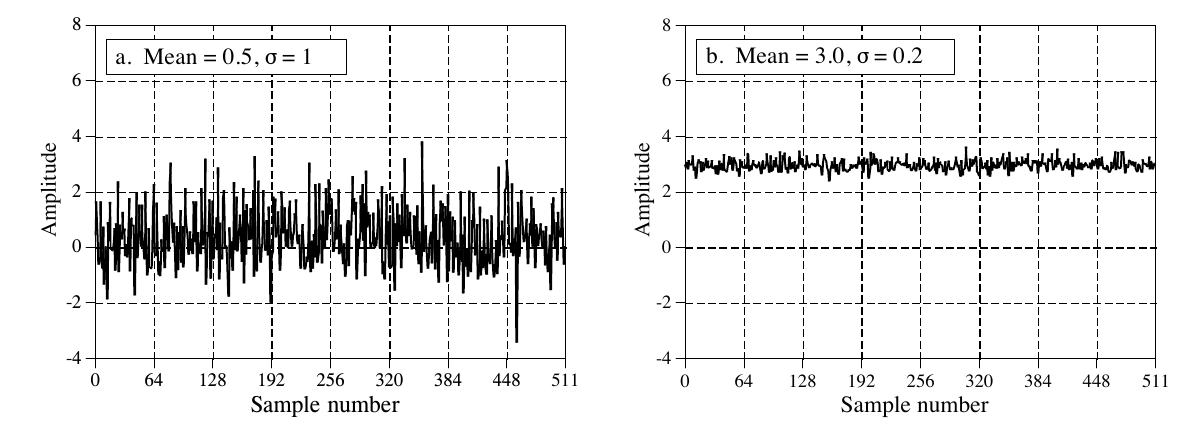
\includegraphics[width=0.992\linewidth,height=0.8\textheight,keepaspectratio]{assets/ch02/fig2-01.png}
\caption*{\textbf{图 2-1　两个均值和标准差不同的数字化信号示例。} （a. 均值 =
0.5，σ = 1；b. 均值 = 3.0，σ = 0.2。图中 Amplitude = 幅度，Sample number
= 采样序号。）}
\end{figure}

\section{均值与标准差}

均值(mean)用 µ（小写希腊字母
mu）表示，是统计学家对信号平均值的行话。它的求法和你想的一样：把所有采样加起来，再除以
N。写成数学形式是：

\textbf{公式 2-1　信号均值的计算。} 信号存放在 \(x_0\) 到 \(x_{N-1}\)
中，i 是遍历这些值的索引，µ 是均值。

\[
\mu = \frac{1}{N}\sum_{i=0}^{N-1} x_i
\]

用文字说：让索引 i 从 0 走到 N−1，把信号的值 \(x_i\)
加起来，最后把总和除以
N。这和下面的式子完全相同：\(\mu = (x_0 + x_1 + x_2 + \cdots + x_{N-1})/N\)。如果你还不熟悉用
Σ（大写希腊字母 sigma）表示求和，请仔细研究这些公式，并和表 2-1
的计算机程序对照。这类求和在 DSP 里比比皆是，你必须彻底弄懂这种记法。

在电子学里，均值通常叫直流(DC, direct current)值。相应地，交流(AC,
alternating
current)指信号围绕均值的波动。如果信号是简单的重复波形，比如正弦波或方波，它的起伏可以用峰峰值(peak-to-peak
amplitude)来描述。可惜大多数采集到的信号没有明确的峰峰值，而是带有随机性，就像图
2-1 中的信号。这时就得用一种更通用的方法，叫标准差(standard
deviation)，记作 σ（小写希腊字母 sigma）。

作为起点，表达式 \(|x_i - \mu|\) 描述了第 i
个采样偏离(deviate)均值多远。把所有单个采样的偏差加起来，再除以采样数
N，就得到信号的平均偏差(average
deviation)。注意求和之前要先对每个偏差取绝对值，否则正负项平均下来会等于零。平均偏差用一个数代表采样离均值的典型距离。它虽然方便直接，但统计学里几乎从不使用。原因是它和信号运作的物理规律不太契合。大多数情况下，重要的参数不是偏离均值的大小，而是这个偏离所代表的功率(power)。例如，随机噪声信号在电子电路中叠加时，合成噪声等于各信号功率之和，而不是幅度之和。

标准差和平均偏差相似，只不过平均的是功率而不是幅度。做法是先把每个偏差平方，再求平均（记住，功率
\dspsym{∝}
电压²）。最后开平方，抵消最初的平方。写成公式，标准差的计算如下：

\textbf{公式 2-2　信号标准差的计算。} 信号存放在 \(x_i\) 中，µ 是由公式
2-1 求出的均值，N 是采样数，σ 是标准差。

\[
\sigma^2 = \frac{1}{N-1}\sum_{i=0}^{N-1} (x_i - \mu)^2
\]

另一种写法：\(\sigma = \sqrt{\big[(x_0-\mu)^2 + (x_1-\mu)^2 + \cdots + (x_{N-1}-\mu)^2\big] / (N-1)}\)。注意这里求平均时除的是
N−1 而不是 N。这是公式里一个微妙的地方，下一节再讨论。\(\sigma^2\)
这一项在统计学里经常出现，它有个名字叫方差(variance)。标准差衡量的是信号偏离均值的波动有多大，方差代表这种波动的功率。另一个你应该熟悉的术语是电子学中常用的均方根(rms,
root-mean-square)值。按定义，标准差只衡量信号的交流部分，而均方根值同时衡量交流和直流成分。如果信号没有直流成分，它的均方根值就等于标准差。图
2-2 展示了几种常见波形的标准差与峰峰值之间的关系。

\begin{figure}[htbp]
\centering
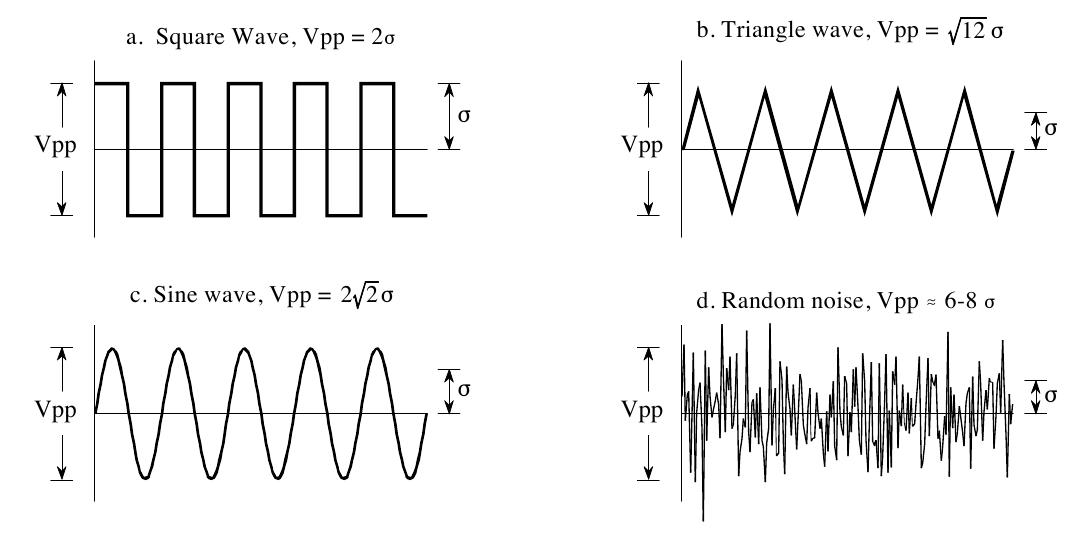
\includegraphics[width=0.900\linewidth,height=0.8\textheight,keepaspectratio]{assets/ch02/fig2-02.png}
\caption*{\textbf{图 2-2　几种常见波形的峰峰值与标准差之比。} 方波的比值是
2；三角波是 \(\sqrt{12} = 3.46\)；正弦波是
\(2\sqrt{2} = 2.83\)。随机噪声没有确切的峰峰值，但大约是标准差的 6 到 8
倍。 （a. 方波(Square Wave)，Vpp = 2σ；b. 三角波(Triangle wave)，Vpp =
\(\sqrt{12}\)σ；c.~正弦波(Sine wave)，Vpp =
\(2\sqrt{2}\)σ；d.~随机噪声(Random noise)，Vpp \dspsym{≈} 6～8σ。Vpp
即峰峰值。）}
\end{figure}

表 2-1 列出了一段用公式 2-1 和 2-2
计算均值和标准差的计算机程序。本书的程序只追求用最直接的方式表达算法，其他因素都排在后面。只要能让程序逻辑更清楚，好的编程技巧也可以不顾。例如：使用简化版的
BASIC、带行号、唯一允许的控制结构是 FOR-NEXT
循环、没有输入输出语句等。可以把这些程序看作理解 DSP
公式的另一种途径，一种看不懂，也许另一种能帮上忙。在 BASIC
里，变量名末尾的 \% 表示它是整数，其他变量都是浮点数。第 4
章会详细讨论这些变量类型。

\textbf{表 2-1}（注释已译成中文）

\begin{Shaded}
\begin{Highlighting}[]
\NormalTok{100 CALCULATION OF THE MEAN AND STANDARD DEVIATION}
\NormalTok{110 \textquotesingle{}}
\NormalTok{120 DIM X[511]                  \textquotesingle{}信号存放在 X[0] 到 X[511]}
\NormalTok{130 N\% = 512                    \textquotesingle{}N\% 是信号的点数}
\NormalTok{140 \textquotesingle{}}
\NormalTok{150 GOSUB XXXX                  \textquotesingle{}虚构的子程序，把信号载入 X[ ]}
\NormalTok{160 \textquotesingle{}}
\NormalTok{170 MEAN = 0                    \textquotesingle{}用公式 2{-}1 求均值}
\NormalTok{180 FOR I\% = 0 TO N\%{-}1}
\NormalTok{190   MEAN = MEAN + X[I\%]}
\NormalTok{200 NEXT I\%}
\NormalTok{210 MEAN = MEAN/N\%}
\NormalTok{220 \textquotesingle{}}
\NormalTok{230 VARIANCE = 0                \textquotesingle{}用公式 2{-}2 求标准差}
\NormalTok{240 FOR I\% = 0 TO N\%{-}1}
\NormalTok{250   VARIANCE = VARIANCE + ( X[I\%] {-} MEAN )\^{}2}
\NormalTok{260 NEXT I\%}
\NormalTok{270 VARIANCE = VARIANCE/(N\%{-}1)}
\NormalTok{280 SD = SQR(VARIANCE)}
\NormalTok{290 \textquotesingle{}}
\NormalTok{300 PRINT MEAN SD               \textquotesingle{}打印算出的均值和标准差}
\NormalTok{310 \textquotesingle{}}
\NormalTok{320 END}
\end{Highlighting}
\end{Shaded}

\textbf{C 实现}（完整可编译版本见 \texttt{c/table2-1\_mean\_sd.c}）：

\begin{Shaded}
\begin{Highlighting}[]
\CommentTok{/* 表 2{-}1  用两遍法计算均值与标准差 */}
\PreprocessorTok{\#include }\ImportTok{\textless{}stdio.h\textgreater{}}
\PreprocessorTok{\#include }\ImportTok{\textless{}math.h\textgreater{}}

\PreprocessorTok{\#define N }\DecValTok{512}\PreprocessorTok{ }\CommentTok{/* 130 N\% = 512，X[0] 到 X[511] */}

\DataTypeTok{static} \DataTypeTok{double}\NormalTok{ x}\OperatorTok{[}\NormalTok{N}\OperatorTok{];}

\CommentTok{/* 150 GOSUB XXXX：原书用一个虚构子程序载入信号，}
\CommentTok{ * 这里改为产生一个可复现的测试信号：正弦 + 均匀噪声 */}
\DataTypeTok{static} \DataTypeTok{void}\NormalTok{ load\_signal}\OperatorTok{(}\DataTypeTok{void}\OperatorTok{)}
\OperatorTok{\{}
    \DataTypeTok{unsigned} \DataTypeTok{int}\NormalTok{ seed }\OperatorTok{=} \DecValTok{12345}\BuiltInTok{u}\OperatorTok{;}
    \ControlFlowTok{for} \OperatorTok{(}\DataTypeTok{int}\NormalTok{ i }\OperatorTok{=} \DecValTok{0}\OperatorTok{;}\NormalTok{ i }\OperatorTok{\textless{}}\NormalTok{ N}\OperatorTok{;}\NormalTok{ i}\OperatorTok{++)} \OperatorTok{\{}
\NormalTok{        seed }\OperatorTok{=}\NormalTok{ seed }\OperatorTok{*} \DecValTok{1664525}\BuiltInTok{u} \OperatorTok{+} \DecValTok{1013904223}\BuiltInTok{u}\OperatorTok{;}             \CommentTok{/* 线性同余随机数 */}
        \DataTypeTok{double}\NormalTok{ noise }\OperatorTok{=} \OperatorTok{((}\NormalTok{seed }\OperatorTok{\textgreater{}\textgreater{}} \DecValTok{8}\OperatorTok{)} \OperatorTok{\&} \BaseNTok{0xFFFF}\OperatorTok{)} \OperatorTok{/} \FloatTok{65535.0}\OperatorTok{;}  \CommentTok{/* 0 到 1 */}
\NormalTok{        noise }\OperatorTok{=} \OperatorTok{(}\NormalTok{noise }\OperatorTok{{-}} \FloatTok{0.5}\OperatorTok{)} \OperatorTok{*} \FloatTok{10.0}\OperatorTok{;}                     \CommentTok{/* {-}5 到 +5 */}
\NormalTok{        x}\OperatorTok{[}\NormalTok{i}\OperatorTok{]} \OperatorTok{=} \FloatTok{20.0} \OperatorTok{*}\NormalTok{ sin}\OperatorTok{(}\FloatTok{2.0} \OperatorTok{*} \FloatTok{3.14159265358979} \OperatorTok{*}\NormalTok{ i }\OperatorTok{/} \FloatTok{64.0}\OperatorTok{)} \OperatorTok{+}\NormalTok{ noise}\OperatorTok{;}
    \OperatorTok{\}}
\OperatorTok{\}}

\DataTypeTok{int}\NormalTok{ main}\OperatorTok{(}\DataTypeTok{void}\OperatorTok{)}
\OperatorTok{\{}
\NormalTok{    load\_signal}\OperatorTok{();}

    \CommentTok{/* 170{-}210：用公式 2{-}1 求均值 */}
    \DataTypeTok{double}\NormalTok{ mean }\OperatorTok{=} \FloatTok{0.0}\OperatorTok{;}
    \ControlFlowTok{for} \OperatorTok{(}\DataTypeTok{int}\NormalTok{ i }\OperatorTok{=} \DecValTok{0}\OperatorTok{;}\NormalTok{ i }\OperatorTok{\textless{}}\NormalTok{ N}\OperatorTok{;}\NormalTok{ i}\OperatorTok{++)} \OperatorTok{\{}
\NormalTok{        mean }\OperatorTok{=}\NormalTok{ mean }\OperatorTok{+}\NormalTok{ x}\OperatorTok{[}\NormalTok{i}\OperatorTok{];}
    \OperatorTok{\}}
\NormalTok{    mean }\OperatorTok{=}\NormalTok{ mean }\OperatorTok{/}\NormalTok{ N}\OperatorTok{;}

    \CommentTok{/* 230{-}280：用公式 2{-}2 求标准差 */}
    \DataTypeTok{double}\NormalTok{ variance }\OperatorTok{=} \FloatTok{0.0}\OperatorTok{;}
    \ControlFlowTok{for} \OperatorTok{(}\DataTypeTok{int}\NormalTok{ i }\OperatorTok{=} \DecValTok{0}\OperatorTok{;}\NormalTok{ i }\OperatorTok{\textless{}}\NormalTok{ N}\OperatorTok{;}\NormalTok{ i}\OperatorTok{++)} \OperatorTok{\{}
        \DataTypeTok{double}\NormalTok{ d }\OperatorTok{=}\NormalTok{ x}\OperatorTok{[}\NormalTok{i}\OperatorTok{]} \OperatorTok{{-}}\NormalTok{ mean}\OperatorTok{;}
\NormalTok{        variance }\OperatorTok{=}\NormalTok{ variance }\OperatorTok{+}\NormalTok{ d }\OperatorTok{*}\NormalTok{ d}\OperatorTok{;}
    \OperatorTok{\}}
\NormalTok{    variance }\OperatorTok{=}\NormalTok{ variance }\OperatorTok{/} \OperatorTok{(}\NormalTok{N }\OperatorTok{{-}} \DecValTok{1}\OperatorTok{);}
    \DataTypeTok{double}\NormalTok{ sd }\OperatorTok{=}\NormalTok{ sqrt}\OperatorTok{(}\NormalTok{variance}\OperatorTok{);}

    \CommentTok{/* 300 PRINT MEAN SD */}
\NormalTok{    printf}\OperatorTok{(}\StringTok{"均值 = }\SpecialCharTok{\%.6f}\StringTok{  标准差 = }\SpecialCharTok{\%.6f\textbackslash{}n}\StringTok{"}\OperatorTok{,}\NormalTok{ mean}\OperatorTok{,}\NormalTok{ sd}\OperatorTok{);}
    \ControlFlowTok{return} \DecValTok{0}\OperatorTok{;}
\OperatorTok{\}}
\end{Highlighting}
\end{Shaded}

这种计算均值和标准差的方法对许多应用都够用，但它有两个局限。第一，如果均值比标准差大得多，公式
2-2 就要把两个非常接近的数相减。这会让计算产生过大的舍入误差(round-off
error)，第 4
章会更详细地讨论这个话题。第二，我们常常希望每采集到一个新采样、加进信号后，就重新计算一次均值和标准差。我们把这种计算叫做滑动统计(running
statistics)。公式 2-1 和 2-2
的方法虽然也能用于滑动统计，但每次重新计算都要用到所有采样，这非常浪费计算能力和内存。

解决这些问题的办法是：对公式 2-1 和 2-2
做变形，得到计算标准差的另一个公式：

\textbf{公式 2-3　用滑动统计计算标准差。} 这个公式和公式 2-2
结果相同，但舍入噪声更小，计算效率更高。信号用三个累加参数表示：N，采样总数；sum，这些采样之和；sum
of squares，这些采样的平方和。均值和标准差都由这三个累加参数算出。

\[
\sigma^2 = \frac{1}{N-1}\left[\sum_{i=0}^{N-1} x_i^2 - \frac{1}{N}\left(\sum_{i=0}^{N-1} x_i\right)^2\right]
\]

或者用更简单的记法：

\[
\sigma^2 = \frac{1}{N-1}\left[\text{sum of squares} - \frac{\text{sum}^2}{N}\right]
\]

在遍历信号的过程中，持续累计三个参数：(1) 已处理的采样数；(2)
这些采样之和；(3)
这些采样的平方和（即把每个采样值平方后加到累计值上）。无论处理了多少个采样，都只需用这三个参数的当前值，就能高效地算出均值和标准差。表
2-2
的程序就是这样，每纳入一个新采样就报告一次均值和标准差。手持计算器求一串数的统计量用的也是这个方法：每输入一个数、按一下
Σ（求和）键，三个参数就更新一次。之后随时都能求出均值和标准差，不必把整串数重新算一遍。

\textbf{表 2-2}（注释已译成中文）

\begin{Shaded}
\begin{Highlighting}[]
\NormalTok{100 \textquotesingle{}MEAN AND STANDARD DEVIATION USING RUNNING STATISTICS}
\NormalTok{110 \textquotesingle{}}
\NormalTok{120 DIM X[511]                  \textquotesingle{}信号存放在 X[0] 到 X[511]}
\NormalTok{130 \textquotesingle{}}
\NormalTok{140 GOSUB XXXX                  \textquotesingle{}虚构的子程序，把信号载入 X[ ]}
\NormalTok{150 \textquotesingle{}}
\NormalTok{160 N\% = 0                      \textquotesingle{}把三个滑动参数清零}
\NormalTok{170 SUM = 0}
\NormalTok{180 SUMSQUARES = 0}
\NormalTok{190 \textquotesingle{}}
\NormalTok{200 FOR I\% = 0 TO 511           \textquotesingle{}逐个遍历信号中的采样}
\NormalTok{210 \textquotesingle{}}
\NormalTok{220   N\% = N\%+1                 \textquotesingle{}更新三个参数}
\NormalTok{230   SUM = SUM + X(I\%)}
\NormalTok{240   SUMSQUARES = SUMSQUARES + X(I\%)\^{}2}
\NormalTok{250 \textquotesingle{}}
\NormalTok{260   MEAN = SUM/N\%             \textquotesingle{}用公式 2{-}3 计算均值和标准差}
\NormalTok{270   VARIANCE = (SUMSQUARES {-} SUM\^{}2/N\%) / (N\%{-}1)}
\NormalTok{280   SD = SQR(VARIANCE)}
\NormalTok{290 \textquotesingle{}}
\NormalTok{300   PRINT MEAN SD             \textquotesingle{}打印滑动均值和标准差}
\NormalTok{310 \textquotesingle{}}
\NormalTok{320 NEXT I\%}
\NormalTok{330 \textquotesingle{}}
\NormalTok{340 END}
\end{Highlighting}
\end{Shaded}

\textbf{C 实现}（完整可编译版本见
\texttt{c/table2-2\_running\_stats.c}）：

\begin{Shaded}
\begin{Highlighting}[]
\CommentTok{/* 表 2{-}2  用滑动统计（running statistics）计算均值与标准差 */}
\PreprocessorTok{\#include }\ImportTok{\textless{}stdio.h\textgreater{}}
\PreprocessorTok{\#include }\ImportTok{\textless{}math.h\textgreater{}}

\PreprocessorTok{\#define N }\DecValTok{512}

\DataTypeTok{static} \DataTypeTok{double}\NormalTok{ x}\OperatorTok{[}\NormalTok{N}\OperatorTok{];}

\CommentTok{/* 140 GOSUB XXXX：载入信号，与表 2{-}1 相同的测试信号 */}
\DataTypeTok{static} \DataTypeTok{void}\NormalTok{ load\_signal}\OperatorTok{(}\DataTypeTok{void}\OperatorTok{)}
\OperatorTok{\{}
    \DataTypeTok{unsigned} \DataTypeTok{int}\NormalTok{ seed }\OperatorTok{=} \DecValTok{12345}\BuiltInTok{u}\OperatorTok{;}
    \ControlFlowTok{for} \OperatorTok{(}\DataTypeTok{int}\NormalTok{ i }\OperatorTok{=} \DecValTok{0}\OperatorTok{;}\NormalTok{ i }\OperatorTok{\textless{}}\NormalTok{ N}\OperatorTok{;}\NormalTok{ i}\OperatorTok{++)} \OperatorTok{\{}
\NormalTok{        seed }\OperatorTok{=}\NormalTok{ seed }\OperatorTok{*} \DecValTok{1664525}\BuiltInTok{u} \OperatorTok{+} \DecValTok{1013904223}\BuiltInTok{u}\OperatorTok{;}
        \DataTypeTok{double}\NormalTok{ noise }\OperatorTok{=} \OperatorTok{((}\NormalTok{seed }\OperatorTok{\textgreater{}\textgreater{}} \DecValTok{8}\OperatorTok{)} \OperatorTok{\&} \BaseNTok{0xFFFF}\OperatorTok{)} \OperatorTok{/} \FloatTok{65535.0}\OperatorTok{;}
\NormalTok{        noise }\OperatorTok{=} \OperatorTok{(}\NormalTok{noise }\OperatorTok{{-}} \FloatTok{0.5}\OperatorTok{)} \OperatorTok{*} \FloatTok{10.0}\OperatorTok{;}
\NormalTok{        x}\OperatorTok{[}\NormalTok{i}\OperatorTok{]} \OperatorTok{=} \FloatTok{20.0} \OperatorTok{*}\NormalTok{ sin}\OperatorTok{(}\FloatTok{2.0} \OperatorTok{*} \FloatTok{3.14159265358979} \OperatorTok{*}\NormalTok{ i }\OperatorTok{/} \FloatTok{64.0}\OperatorTok{)} \OperatorTok{+}\NormalTok{ noise}\OperatorTok{;}
    \OperatorTok{\}}
\OperatorTok{\}}

\DataTypeTok{int}\NormalTok{ main}\OperatorTok{(}\DataTypeTok{void}\OperatorTok{)}
\OperatorTok{\{}
\NormalTok{    load\_signal}\OperatorTok{();}

    \CommentTok{/* 160{-}180：三个滑动参数清零 */}
    \DataTypeTok{int}\NormalTok{ n }\OperatorTok{=} \DecValTok{0}\OperatorTok{;}
    \DataTypeTok{double}\NormalTok{ sum }\OperatorTok{=} \FloatTok{0.0}\OperatorTok{;}
    \DataTypeTok{double}\NormalTok{ sumsquares }\OperatorTok{=} \FloatTok{0.0}\OperatorTok{;}

    \CommentTok{/* 200 FOR I\% = 0 TO 511 */}
    \ControlFlowTok{for} \OperatorTok{(}\DataTypeTok{int}\NormalTok{ i }\OperatorTok{=} \DecValTok{0}\OperatorTok{;}\NormalTok{ i }\OperatorTok{\textless{}}\NormalTok{ N}\OperatorTok{;}\NormalTok{ i}\OperatorTok{++)} \OperatorTok{\{}
        \CommentTok{/* 220{-}240：更新三个参数 */}
\NormalTok{        n }\OperatorTok{=}\NormalTok{ n }\OperatorTok{+} \DecValTok{1}\OperatorTok{;}
\NormalTok{        sum }\OperatorTok{=}\NormalTok{ sum }\OperatorTok{+}\NormalTok{ x}\OperatorTok{[}\NormalTok{i}\OperatorTok{];}
\NormalTok{        sumsquares }\OperatorTok{=}\NormalTok{ sumsquares }\OperatorTok{+}\NormalTok{ x}\OperatorTok{[}\NormalTok{i}\OperatorTok{]} \OperatorTok{*}\NormalTok{ x}\OperatorTok{[}\NormalTok{i}\OperatorTok{];}

        \CommentTok{/* 260{-}280：用公式 2{-}3 计算均值和标准差}
\CommentTok{         * 注意：BASIC 原文在 n = 1 时会除以 (n{-}1) = 0，}
\CommentTok{         * 这里加一个判断，只有两个及以上采样时才计算。 */}
        \DataTypeTok{double}\NormalTok{ mean }\OperatorTok{=}\NormalTok{ sum }\OperatorTok{/}\NormalTok{ n}\OperatorTok{;}
        \DataTypeTok{double}\NormalTok{ sd }\OperatorTok{=} \FloatTok{0.0}\OperatorTok{;}
        \ControlFlowTok{if} \OperatorTok{(}\NormalTok{n }\OperatorTok{\textgreater{}} \DecValTok{1}\OperatorTok{)} \OperatorTok{\{}
            \DataTypeTok{double}\NormalTok{ variance }\OperatorTok{=} \OperatorTok{(}\NormalTok{sumsquares }\OperatorTok{{-}}\NormalTok{ sum }\OperatorTok{*}\NormalTok{ sum }\OperatorTok{/}\NormalTok{ n}\OperatorTok{)} \OperatorTok{/} \OperatorTok{(}\NormalTok{n }\OperatorTok{{-}} \DecValTok{1}\OperatorTok{);}
\NormalTok{            sd }\OperatorTok{=}\NormalTok{ sqrt}\OperatorTok{(}\NormalTok{variance}\OperatorTok{);}
        \OperatorTok{\}}

        \CommentTok{/* 300 PRINT MEAN SD */}
        \ControlFlowTok{if} \OperatorTok{(}\NormalTok{i }\OperatorTok{==} \DecValTok{0} \OperatorTok{||}\NormalTok{ i }\OperatorTok{==}\NormalTok{ N }\OperatorTok{{-}} \DecValTok{1}\OperatorTok{)} \OperatorTok{\{}
\NormalTok{            printf}\OperatorTok{(}\StringTok{"第 }\SpecialCharTok{\%d}\StringTok{ 个采样后：均值 = }\SpecialCharTok{\%.6f}\StringTok{  标准差 = }\SpecialCharTok{\%.6f\textbackslash{}n}\StringTok{"}\OperatorTok{,}
\NormalTok{                   n}\OperatorTok{,}\NormalTok{ mean}\OperatorTok{,}\NormalTok{ sd}\OperatorTok{);}
        \OperatorTok{\}}
    \OperatorTok{\}}
    \ControlFlowTok{return} \DecValTok{0}\OperatorTok{;}
\OperatorTok{\}}
\end{Highlighting}
\end{Shaded}

结束均值和标准差的讨论之前，还要提两个术语。在某些情况下，均值描述的是被测量的东西，而标准差代表噪声和其他干扰。这时标准差本身并不重要，重要的是它和均值的比较。由此产生了信噪比(SNR,
signal-to-noise
ratio)这个术语，它等于均值除以标准差。另一个术语是变异系数(CV,
coefficient of variation)，定义为标准差除以均值，再乘以 100\%。例如，CV
为 2\% 的信号（或其他一组测量值），SNR 是 50。数据越好，SNR 越高，CV
越低。

\section{信号与其背后的过程}

统计是解释数值数据（比如采集到的信号）的科学。相比之下，DSP
用概率来理解产生信号的过程。两者联系紧密，但「采集到的信号」与「背后的过程(underlying
process)」之间的区别，是许多 DSP 技术的关键。

例如，设想把硬币抛 1000 次，生成一个 1000
点的信号。正面朝上，对应的采样取值 1；反面朝上，取值
0。产生这个信号的过程，均值恰好是
0.5，这是由每种结果的相对概率决定的：50\% 正面，50\% 反面。然而，实际的
1000 点信号均值恰好是 0.5 的可能性很小。随机性会让每次生成信号时 1 和 0
的个数略有不同。背后过程的概率是不变的，但每次重复实验，采集到的信号的统计量都会变。实际数据中的这种随机不规则性，有统计变异(statistical
variation)、统计涨落(statistical fluctuation)、统计噪声(statistical
noise)等叫法。

这就带来一个小小的两难。看到「均值」和「标准差」这些词时，你怎么知道作者说的是实际信号的统计量，还是产生信号的背后过程的概率？遗憾的是，只能靠上下文判断。并不是统计和概率中所有术语都这样。例如，直方图和概率质量函数（下一节讨论）就是一对对应的概念，各有各的名字。

现在回到计算标准差的公式
2-2。前面说过，这个公式在计算偏差平方的平均值时，除的是 N−1 而不是
N。要理解为什么，设想你想求某个产生信号的过程的均值和标准差。为此，你从这个过程采集了一个
N 点的信号，用公式 2-1
算出信号的均值。你可以用它来估计背后过程的均值，但你知道统计噪声会带来误差。特别地，对随机信号来说，N
个点的均值与背后过程的均值之间的典型误差为：

\textbf{公式 2-4　用有限的 N 个采样计算背后过程均值时的典型误差。} 参数
σ 是标准差。

\[
\text{典型误差} = \frac{\sigma}{N^{1/2}}
\]

如果 N
很小，算出的均值里的统计噪声就会很大。换句话说，你掌握的数据不够，没法恰当地刻画这个过程。N
越大，预期误差就越小。概率论的一个里程碑------强大数定律(Strong Law of
Large Numbers)------保证了当 N 趋于无穷时误差变为零。

下一步，我们想计算采集信号的标准差，并用它来估计背后过程的标准差。问题就出在这里。用公式
2-2 计算标准差之前，你得先知道均值 µ。可你并不知道背后过程的均值，只知道
N
点信号的均值，而它含有统计噪声带来的误差。这个误差往往会让算出的标准差偏小。为了补偿，把
N 换成 N−1。N 很大时，这点差别无关紧要；N
很小时，这样替换能更准确地估计背后过程的标准差。换句话说，公式 2-2
是对背后过程标准差的估计。如果公式里除以
N，得到的就是采集信号本身的标准差。

\begin{figure}[htbp]
\centering
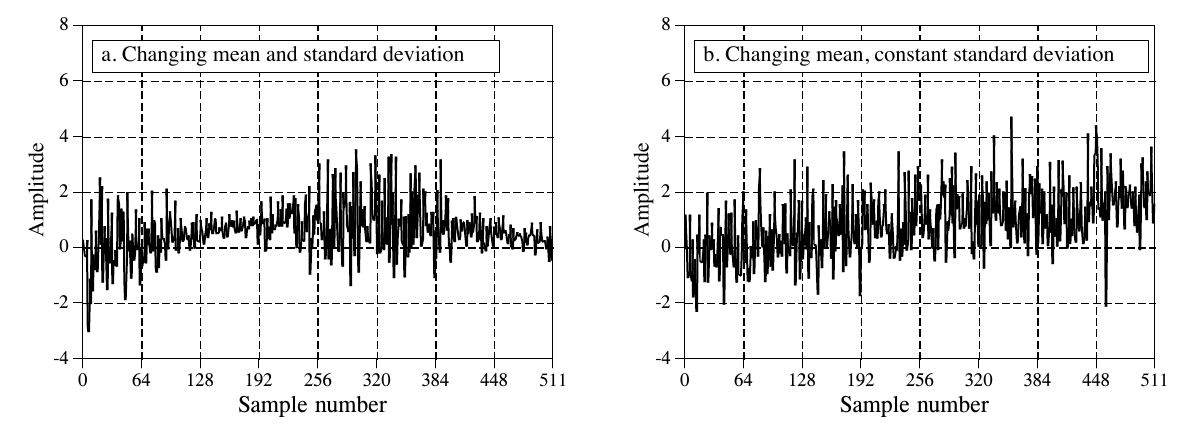
\includegraphics[width=0.992\linewidth,height=0.8\textheight,keepaspectratio]{assets/ch02/fig2-03.png}
\caption*{\textbf{图 2-3　由非平稳过程产生的信号示例。} (a)
中均值和标准差都在变。(b) 中标准差保持为常数 1，而均值从 0 变到
2。常用的分析方法是把这类信号切成短段，逐段计算统计量。 （a.
均值和标准差都在变化(Changing mean and standard deviation)；b.
均值变化、标准差不变(Changing mean, constant standard deviation)。）}
\end{figure}

为了说明这些想法，看看图 2-3
中的信号，问问自己：这些信号里的变化，是统计噪声造成的，还是背后的过程在变？不难让自己相信，这些变化太大了，不可能是随机造成的，一定和背后的过程有关。像这样特性会改变的过程称为非平稳(nonstationary)过程。相比之下，前面图
2-1 的信号是由平稳(stationary)过程产生的，其中的变化完全来自统计噪声。图
2-3b
说明了非平稳信号的一个常见问题：缓慢变化的均值会干扰标准差的计算。在这个例子中，信号在短区间内的标准差是
1，但整个信号的标准差是
1.16。把信号切成短段、逐段计算统计量，几乎可以消除这个误差。如果需要，还可以把各段的标准差平均成一个值。

\section{直方图、概率质量函数与概率密度函数}

假设我们给计算机接上一个 8 比特模数转换器，采集某个信号的 256,000
个采样。举个例子，图 2-4a 是这个数据集中可能的 128
个采样。每个采样的值是 256 种可能（0 到
255）之一。直方图(histogram)显示的是：信号中取每种可能值的采样各有多少个。图
(b) 是 (a) 中 128 个采样的直方图。例如，有 2 个采样的值是 110，有 8
个采样的值是 131，有 0 个采样的值是 170，等等。我们用 \(H_i\)
表示直方图，i 是从 0 到 M−1 的索引，M
是每个采样可能取值的个数。例如，\(H_{50}\) 是值为 50 的采样个数。图 (c)
是用全部数据集（全部 256k
个点）得到的直方图。可以看到，采样越多，样子就平滑得多。和均值一样，直方图的统计噪声（粗糙程度）与所用采样数的平方根成反比。

\begin{figure}[htbp]
\centering
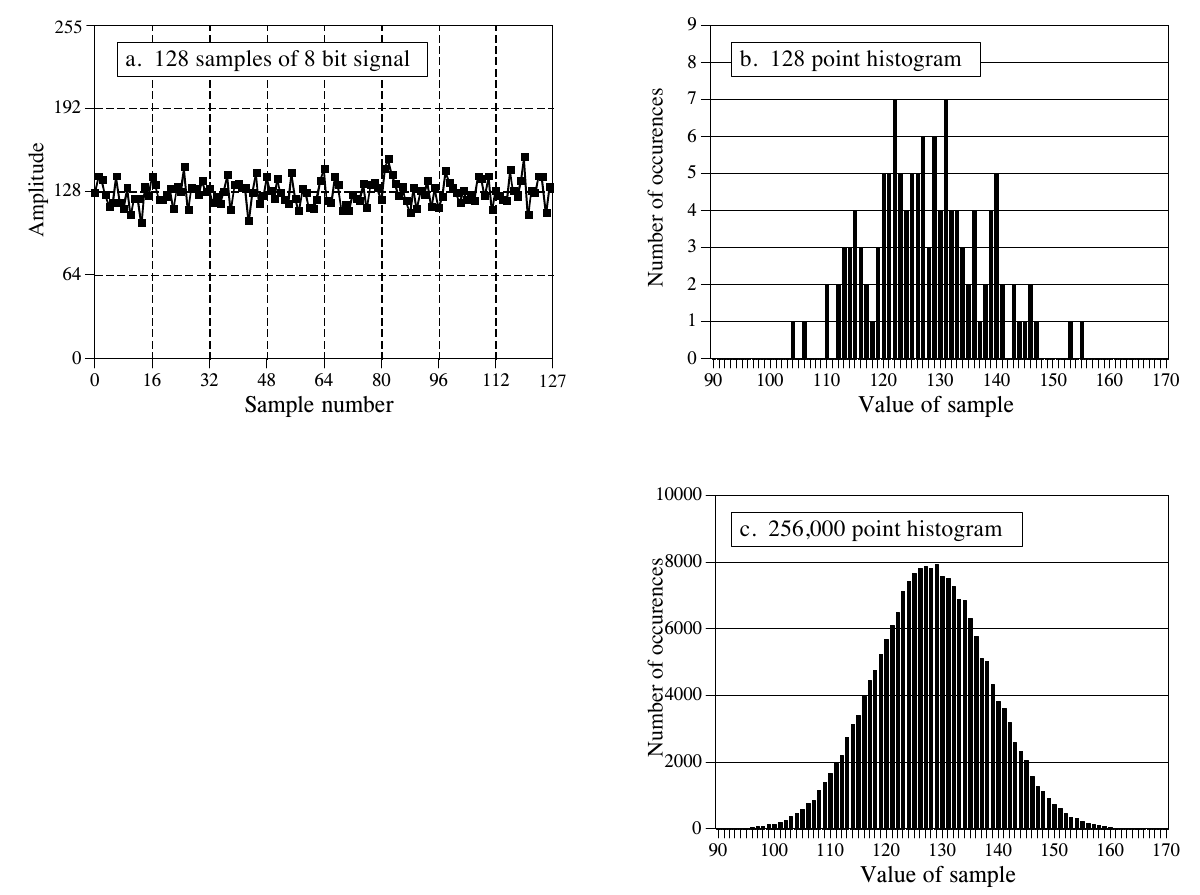
\includegraphics[width=1.000\linewidth,height=0.8\textheight,keepaspectratio]{assets/ch02/fig2-04.png}
\caption*{\textbf{图 2-4　直方图示例。} 图 (a) 是从一个很长的信号中取出的 128
个采样，每个采样是 0 到 255 之间的整数。图 (b) 和 (c) 分别是用信号中 128
个和 256,000 个采样得到的直方图。可以看到，采样越多，直方图越平滑。 （a.
8 比特信号的 128 个采样；b. 128 点直方图；c.~256,000 点直方图。Number of
occurences = 出现次数，Value of sample = 采样值。）}
\end{figure}

根据定义，直方图所有值之和必然等于信号的点数：

\textbf{公式 2-5　直方图所有值之和等于信号的点数。} 式中 \(H_i\)
是直方图，N 是信号的点数，M 是直方图的点数。

\[
N = \sum_{i=0}^{M-1} H_i
\]

直方图可以用来高效地计算超大数据集的均值和标准差。这对图像尤其重要，因为一幅图像可能有几百万个采样。直方图把值相同的采样归为一组，这样计算统计量时只需处理少数几组，而不必处理大量单个采样。用这种方法，由直方图计算均值和标准差的公式是：

\textbf{公式 2-6　由直方图计算均值。}
可以看作把值相同的采样归成组，再对每组使用公式 2-1。

\[
\mu = \frac{1}{N}\sum_{i=0}^{M-1} i\,H_i
\]

\textbf{公式 2-7　由直方图计算标准差。} 思路和公式 2-2
相同，只是对值相同的所有采样一次性处理。

\[
\sigma^2 = \frac{1}{N-1}\sum_{i=0}^{M-1} (i-\mu)^2 H_i
\]

表 2-3
是用这些公式计算直方图、均值和标准差的程序。计算直方图非常快，因为只需要索引和自增。相比之下，计算均值和标准差需要耗时的加法和乘法运算。这个算法的策略是：只对直方图里的少数几个数做这些慢运算，而不是对信号里的大量采样做。这使它比前面介绍的方法快得多。对于很长的信号、在通用计算机上计算时，大约能快十倍。

\textbf{表 2-3}（注释已译成中文）

\begin{Shaded}
\begin{Highlighting}[]
\NormalTok{100 \textquotesingle{}CALCULATION OF THE HISTOGRAM, MEAN, AND STANDARD DEVIATION}
\NormalTok{110 \textquotesingle{}}
\NormalTok{120 DIM X\%[25000]               \textquotesingle{}X\%[0] 到 X\%[25000] 存放待处理的信号}
\NormalTok{130 DIM H\%[255]                 \textquotesingle{}H\%[0] 到 H\%[255] 存放直方图}
\NormalTok{140 N\% = 25001                  \textquotesingle{}设置信号的点数}
\NormalTok{150 \textquotesingle{}}
\NormalTok{160 FOR I\% = 0 TO 255           \textquotesingle{}把直方图清零，以便用作累加器}
\NormalTok{170   H\%[I\%] = 0}
\NormalTok{180 NEXT I\%}
\NormalTok{190 \textquotesingle{}}
\NormalTok{200 GOSUB XXXX                  \textquotesingle{}虚构的子程序，把信号载入 X\%[ ]}
\NormalTok{210 \textquotesingle{}}
\NormalTok{220 FOR I\% = 0 TO 25000         \textquotesingle{}计算 25001 个点的直方图}
\NormalTok{230   H\%[ X\%[I\%] ] = H\%[ X\%[I\%] ] + 1}
\NormalTok{240 NEXT I\%}
\NormalTok{250 \textquotesingle{}}
\NormalTok{260 MEAN = 0                    \textquotesingle{}用公式 2{-}6 计算均值}
\NormalTok{270 FOR I\% = 0 TO 255}
\NormalTok{280   MEAN = MEAN + I\% * H\%[I\%]}
\NormalTok{290 NEXT I\%}
\NormalTok{300 MEAN = MEAN / N\%}
\NormalTok{310 \textquotesingle{}}
\NormalTok{320 VARIANCE = 0                \textquotesingle{}用公式 2{-}7 计算标准差}
\NormalTok{330 FOR I\% = 0 TO 255}
\NormalTok{340   VARIANCE = VARIANCE + H[I\%] * (I\%{-}MEAN)\^{}2}
\NormalTok{350 NEXT I\%}
\NormalTok{360 VARIANCE = VARIANCE / (N\%{-}1)}
\NormalTok{370 SD = SQR(VARIANCE)}
\NormalTok{380 \textquotesingle{}}
\NormalTok{390 PRINT MEAN SD               \textquotesingle{}打印算出的均值和标准差}
\NormalTok{400 \textquotesingle{}}
\NormalTok{410 END}
\end{Highlighting}
\end{Shaded}

\textbf{C 实现}（完整可编译版本见
\texttt{c/table2-3\_histogram\_stats.c}）：

\begin{Shaded}
\begin{Highlighting}[]
\CommentTok{/* 表 2{-}3  用直方图计算均值与标准差 */}
\PreprocessorTok{\#include }\ImportTok{\textless{}stdio.h\textgreater{}}
\PreprocessorTok{\#include }\ImportTok{\textless{}math.h\textgreater{}}

\PreprocessorTok{\#define NUM\_POINTS }\DecValTok{25001}\PreprocessorTok{ }\CommentTok{/* 140 N\% = 25001，X\%[0] 到 X\%[25000] */}
\PreprocessorTok{\#define NUM\_LEVELS }\DecValTok{256}\PreprocessorTok{   }\CommentTok{/* 150 DIM H\%[255]，8 比特信号 */}

\DataTypeTok{static} \DataTypeTok{int}\NormalTok{ x}\OperatorTok{[}\NormalTok{NUM\_POINTS}\OperatorTok{];}
\DataTypeTok{static} \DataTypeTok{int}\NormalTok{ h}\OperatorTok{[}\NormalTok{NUM\_LEVELS}\OperatorTok{];}

\CommentTok{/* 200 GOSUB XXXX：载入整数信号，这里用 0 到 255 均匀分布的测试数据 */}
\DataTypeTok{static} \DataTypeTok{void}\NormalTok{ load\_signal}\OperatorTok{(}\DataTypeTok{void}\OperatorTok{)}
\OperatorTok{\{}
    \DataTypeTok{unsigned} \DataTypeTok{int}\NormalTok{ seed }\OperatorTok{=} \DecValTok{54321}\BuiltInTok{u}\OperatorTok{;}
    \ControlFlowTok{for} \OperatorTok{(}\DataTypeTok{int}\NormalTok{ i }\OperatorTok{=} \DecValTok{0}\OperatorTok{;}\NormalTok{ i }\OperatorTok{\textless{}}\NormalTok{ NUM\_POINTS}\OperatorTok{;}\NormalTok{ i}\OperatorTok{++)} \OperatorTok{\{}
\NormalTok{        seed }\OperatorTok{=}\NormalTok{ seed }\OperatorTok{*} \DecValTok{1664525}\BuiltInTok{u} \OperatorTok{+} \DecValTok{1013904223}\BuiltInTok{u}\OperatorTok{;}
\NormalTok{        x}\OperatorTok{[}\NormalTok{i}\OperatorTok{]} \OperatorTok{=} \OperatorTok{(}\DataTypeTok{int}\OperatorTok{)((}\NormalTok{seed }\OperatorTok{\textgreater{}\textgreater{}} \DecValTok{8}\OperatorTok{)} \OperatorTok{\%}\NormalTok{ NUM\_LEVELS}\OperatorTok{);}
    \OperatorTok{\}}
\OperatorTok{\}}

\DataTypeTok{int}\NormalTok{ main}\OperatorTok{(}\DataTypeTok{void}\OperatorTok{)}
\OperatorTok{\{}
    \CommentTok{/* 160{-}180：把直方图清零，以便用作累加器 */}
    \ControlFlowTok{for} \OperatorTok{(}\DataTypeTok{int}\NormalTok{ i }\OperatorTok{=} \DecValTok{0}\OperatorTok{;}\NormalTok{ i }\OperatorTok{\textless{}}\NormalTok{ NUM\_LEVELS}\OperatorTok{;}\NormalTok{ i}\OperatorTok{++)} \OperatorTok{\{}
\NormalTok{        h}\OperatorTok{[}\NormalTok{i}\OperatorTok{]} \OperatorTok{=} \DecValTok{0}\OperatorTok{;}
    \OperatorTok{\}}

\NormalTok{    load\_signal}\OperatorTok{();}

    \CommentTok{/* 220{-}240：计算 25001 个点的直方图 */}
    \ControlFlowTok{for} \OperatorTok{(}\DataTypeTok{int}\NormalTok{ i }\OperatorTok{=} \DecValTok{0}\OperatorTok{;}\NormalTok{ i }\OperatorTok{\textless{}}\NormalTok{ NUM\_POINTS}\OperatorTok{;}\NormalTok{ i}\OperatorTok{++)} \OperatorTok{\{}
\NormalTok{        h}\OperatorTok{[}\NormalTok{x}\OperatorTok{[}\NormalTok{i}\OperatorTok{]]} \OperatorTok{=}\NormalTok{ h}\OperatorTok{[}\NormalTok{x}\OperatorTok{[}\NormalTok{i}\OperatorTok{]]} \OperatorTok{+} \DecValTok{1}\OperatorTok{;}
    \OperatorTok{\}}

    \CommentTok{/* 260{-}300：用公式 2{-}6 计算均值 */}
    \DataTypeTok{double}\NormalTok{ mean }\OperatorTok{=} \FloatTok{0.0}\OperatorTok{;}
    \ControlFlowTok{for} \OperatorTok{(}\DataTypeTok{int}\NormalTok{ i }\OperatorTok{=} \DecValTok{0}\OperatorTok{;}\NormalTok{ i }\OperatorTok{\textless{}}\NormalTok{ NUM\_LEVELS}\OperatorTok{;}\NormalTok{ i}\OperatorTok{++)} \OperatorTok{\{}
\NormalTok{        mean }\OperatorTok{=}\NormalTok{ mean }\OperatorTok{+}\NormalTok{ i }\OperatorTok{*}\NormalTok{ h}\OperatorTok{[}\NormalTok{i}\OperatorTok{];}
    \OperatorTok{\}}
\NormalTok{    mean }\OperatorTok{=}\NormalTok{ mean }\OperatorTok{/}\NormalTok{ NUM\_POINTS}\OperatorTok{;}

    \CommentTok{/* 320{-}370：用公式 2{-}7 计算标准差 */}
    \DataTypeTok{double}\NormalTok{ variance }\OperatorTok{=} \FloatTok{0.0}\OperatorTok{;}
    \ControlFlowTok{for} \OperatorTok{(}\DataTypeTok{int}\NormalTok{ i }\OperatorTok{=} \DecValTok{0}\OperatorTok{;}\NormalTok{ i }\OperatorTok{\textless{}}\NormalTok{ NUM\_LEVELS}\OperatorTok{;}\NormalTok{ i}\OperatorTok{++)} \OperatorTok{\{}
        \DataTypeTok{double}\NormalTok{ d }\OperatorTok{=}\NormalTok{ i }\OperatorTok{{-}}\NormalTok{ mean}\OperatorTok{;}
\NormalTok{        variance }\OperatorTok{=}\NormalTok{ variance }\OperatorTok{+}\NormalTok{ h}\OperatorTok{[}\NormalTok{i}\OperatorTok{]} \OperatorTok{*}\NormalTok{ d }\OperatorTok{*}\NormalTok{ d}\OperatorTok{;}
    \OperatorTok{\}}
\NormalTok{    variance }\OperatorTok{=}\NormalTok{ variance }\OperatorTok{/} \OperatorTok{(}\NormalTok{NUM\_POINTS }\OperatorTok{{-}} \DecValTok{1}\OperatorTok{);}
    \DataTypeTok{double}\NormalTok{ sd }\OperatorTok{=}\NormalTok{ sqrt}\OperatorTok{(}\NormalTok{variance}\OperatorTok{);}

    \CommentTok{/* 390 PRINT MEAN SD */}
\NormalTok{    printf}\OperatorTok{(}\StringTok{"均值 = }\SpecialCharTok{\%.6f}\StringTok{  标准差 = }\SpecialCharTok{\%.6f\textbackslash{}n}\StringTok{"}\OperatorTok{,}\NormalTok{ mean}\OperatorTok{,}\NormalTok{ sd}\OperatorTok{);}
    \ControlFlowTok{return} \DecValTok{0}\OperatorTok{;}
\OperatorTok{\}}
\end{Highlighting}
\end{Shaded}

「采集到的信号是背后过程的带噪版本」这个观念非常重要，重要到有些概念为此取了不同的名字。直方图是由采集到的信号得到的。背后过程对应的曲线叫概率质量函数(pmf,
probability mass function)。直方图总是用有限个采样算出来的，而 pmf
是用无限多个采样才能得到的结果。pmf
可以从直方图估计（推断）出来，也可以用某种数学方法推导出来，比如抛硬币的例子。

图 2-5 展示了一个 pmf
的例子，以及和它对应的一个可能的直方图。理解这些概念的关键在于纵轴的单位。前面说过，直方图的纵轴是某个值在信号中出现的次数。pmf
的纵轴包含类似的信息，只不过是以比例表示的。换句话说，把直方图的每个值除以采样总数，就得到
pmf 的近似。这意味着 pmf 的每个值都必须在 0 到 1 之间，并且 pmf
所有值之和等于 1。

pmf 之所以重要，是因为它描述了生成某个值的概率。例如，设想一个 pmf 如图
2-5b 的信号，比如前面图 2-4a
那样的信号。从这个信号中取一个采样，它的值为 120 的概率是多少？图 2-5b
给出了答案：0.03，大约 34 次里有 1 次。随机选一个采样，它的值大于 150
的概率是多少？把 pmf 在 151、152、153、\ldots、255 处的值加起来，答案是
0.0122，大约 82 次里有 1 次。因此，平均每 82
个点，预计会有一个点的值超过 150。任意一个采样的值在 0 到 255
之间的概率是多少？把直方图所有值加起来，得到概率
1.00，即这件事必然发生。

\begin{figure}[htbp]
\centering
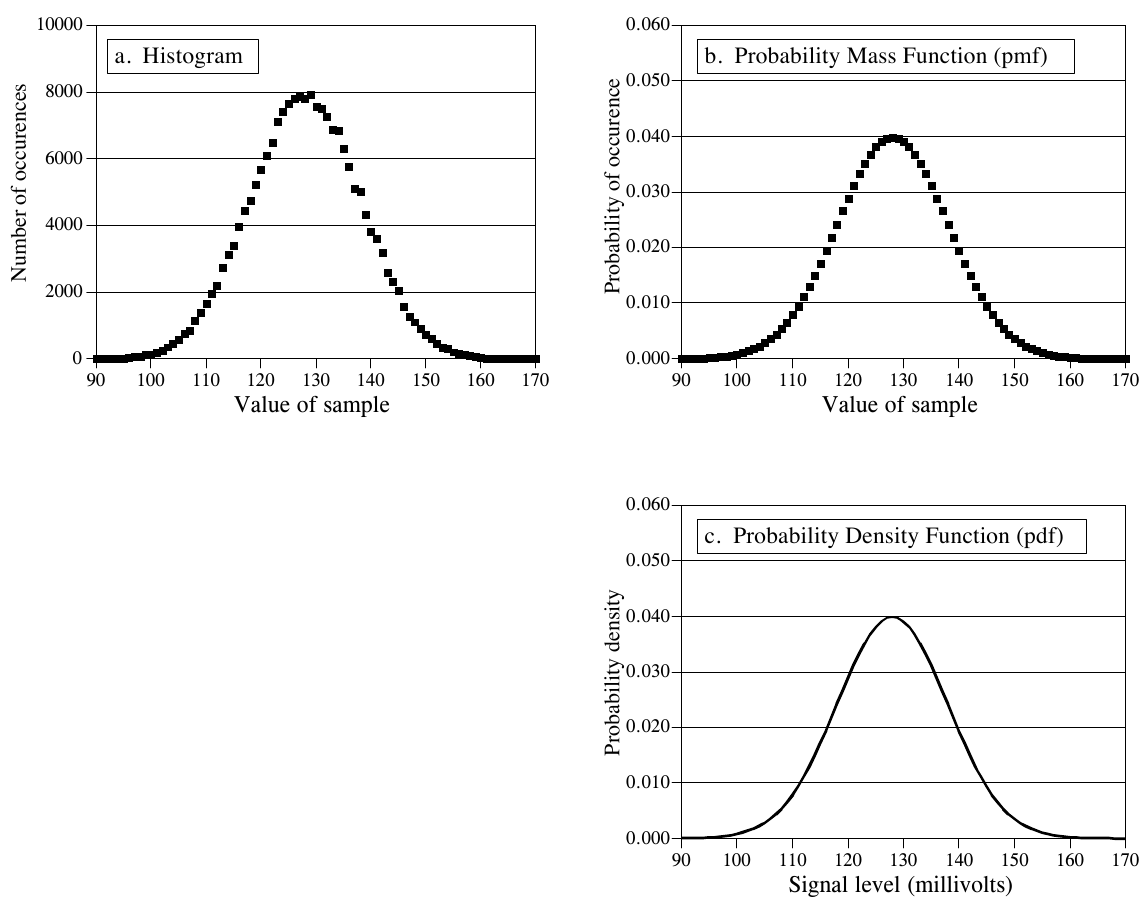
\includegraphics[width=0.950\linewidth,height=0.8\textheight,keepaspectratio]{assets/ch02/fig2-05.png}
\caption*{\textbf{图 2-5　(a) 直方图、(b) 概率质量函数(pmf) 与 (c)
概率密度函数(pdf) 之间的关系。} 直方图由有限个采样计算得到。pmf
描述背后过程的概率。pdf 与 pmf 相似，但用于连续信号而不是离散信号。虽然
(b) 和 (c) 的纵轴数值相同（0 到
0.06），这只是本例的巧合。三条曲线的高度分别由以下条件决定：(a)
直方图所有值之和等于信号的采样数；(b) pmf 所有值之和等于 1；(c) pdf
曲线下的面积等于 1。 （a. Histogram = 直方图；b. Probability Mass
Function = 概率质量函数；c.~Probability Density Function =
概率密度函数。Probability of occurence = 出现概率，Probability density =
概率密度，Signal level (millivolts) = 信号电平（毫伏）。）}
\end{figure}

直方图和 pmf
只能用于离散数据，比如存放在计算机里的数字化信号。连续信号（比如模拟电路中的电压）也有类似的概念。概率密度函数(pdf,
probability density function)，也叫概率分布函数(probability distribution
function)，它之于连续信号，就像概率质量函数之于离散信号。例如，设想一个模拟信号经过模数转换器，得到图
2-4a 的数字化信号。为简单起见，假设 0 到 255 毫伏之间的电压被数字化成 0
到 255 之间的数字。这个数字信号的 pmf 如图 2-5b
中的标记点所示。类似地，模拟信号的 pdf 如 (c)
中的连续曲线所示，表明信号可以取连续范围内的值，比如电子电路中的电压。

pdf 纵轴的单位是概率密度(probability density)，而不只是概率。例如，pdf
在 120.5 处为 0.03，并不意味着电压为 120.5 毫伏的时间占
3\%。事实上，连续信号恰好等于 120.5
毫伏的概率无穷小。这是因为信号要在无穷多个可能的值之间分配它的时间：120.49997、120.49998、120.49999
等等。信号恰好等于 120.50000\ldots{} 的机会确实微乎其微！

要计算概率，需要把概率密度乘以一个取值范围。例如，信号在任意给定时刻处于
120 到 121 之间的概率是：(121−120) × 0.03 = 0.03。信号处于 120.4 到
120.5 之间的概率是：(120.5−120.4) × 0.03 = 0.003，依此类推。如果 pdf
在关心的范围内不是常数，乘法就变成 pdf
在该范围上的积分。换句话说，就是给定数值所界定的 pdf
曲线下的面积。由于信号总得取某个值，pdf 曲线下的总面积，即从 −\dspsym{∞}
到 +\dspsym{∞} 的积分，总是等于 1。这就像 pmf 所有值之和等于
1、直方图所有值之和等于 N 一样。

直方图、pmf 和 pdf
是非常相似的概念。数学家总能把它们分得清清楚楚，但你会经常看到许多科学家和工程师把它们混用（因此用错）。图
2-6 展示了三种连续波形及其
pdf。如果它们是离散信号（把横轴标注改成「采样序号」即可表示），就要用
pmf。

\begin{figure}[htbp]
\centering
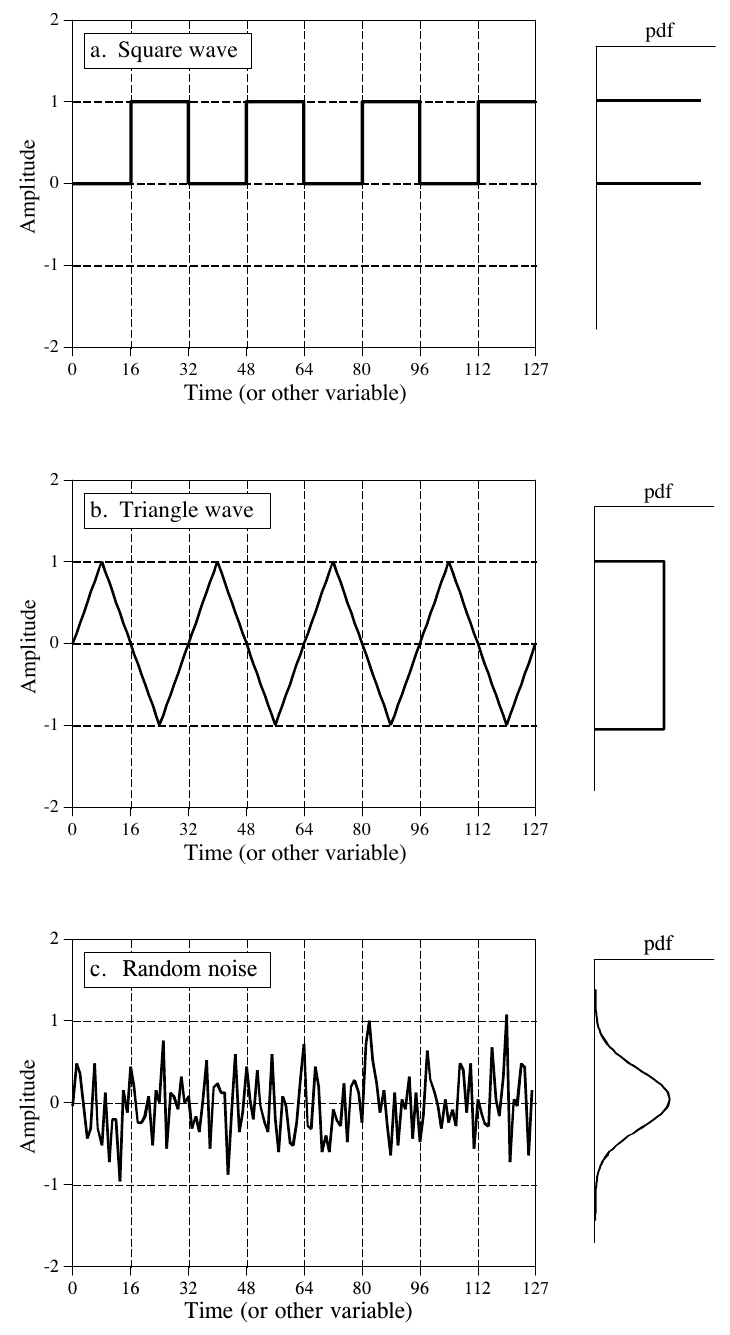
\includegraphics[width=0.608\linewidth,height=0.8\textheight,keepaspectratio]{assets/ch02/fig2-06.png}
\caption*{\textbf{图 2-6　三种常见波形及其概率密度函数。} 像这些例子一样，pdf
图常被旋转四分之一圈，放在它所描述的信号旁边。(a) 方波的 pdf
由两个无限窄的尖峰组成，对应信号只有两个可能的值。(b) 三角波的 pdf
在一个范围内是常数，常称为均匀分布(uniform distribution)。(c) 随机噪声的
pdf 最有意思，是一条钟形曲线，叫高斯分布(Gaussian)。 （a. Square wave =
方波；b. Triangle wave = 三角波；c.~Random noise = 随机噪声。Time (or
other variable) = 时间（或其他变量）。）}
\end{figure}

当每个采样可能取的电平数远多于信号的采样数时，计算直方图就会出问题。用浮点数表示的信号总是如此，因为每个采样都以小数形式存储。例如，整数表示可能要求采样值是
3 或 4，而浮点数允许 3 和 4
之间有几百万个可能的小数值。前面介绍的计算直方图的方法，是统计取每个可能量化电平的采样个数。浮点数据没法这样做，因为要考虑的可能电平有几十亿个。更糟的是，这些可能电平中几乎都没有对应的采样。例如，设想一个
10,000
个采样的信号，每个采样有十亿个可能的值。常规直方图将有十亿个数据点，其中除了大约
10,000 个以外，全都是零。

解决这些问题的技术叫分箱(binning)。做法是：随意选定直方图的长度为某个方便的数，比如
1000
个点，这些点通常叫做箱(bins)。每个箱的值代表信号中落在某个取值范围内的采样总数。例如，设想一个浮点信号的值在
0.0 到 10.0 之间，直方图有 1000 个箱。第 0 个箱是值在 0 到 0.01
之间的采样个数，第 1 个箱是值在 0.01 到 0.02
之间的采样个数，依此类推，直到第 999 个箱，是值在 9.99 到 10.0
之间的采样个数。表 2-4 给出了按这种方式计算分箱直方图的程序。

\textbf{表 2-4}（注释已译成中文）

\begin{Shaded}
\begin{Highlighting}[]
\NormalTok{100 \textquotesingle{}CALCULATION OF BINNED HISTOGRAM}
\NormalTok{110 \textquotesingle{}}
\NormalTok{120 DIM X[25000]                \textquotesingle{}X[0] 到 X[25000] 存放浮点信号，}
\NormalTok{130 \textquotesingle{}                           \textquotesingle{}每个采样的范围是 0.0 到 10.0}
\NormalTok{140 DIM H\%[999]                 \textquotesingle{}H\%[0] 到 H\%[999] 存放分箱直方图}
\NormalTok{150 \textquotesingle{}}
\NormalTok{160 FOR I\% = 0 TO 999           \textquotesingle{}把分箱直方图清零，以便用作累加器}
\NormalTok{170   H\%[I\%] = 0}
\NormalTok{180 NEXT I\%}
\NormalTok{190 \textquotesingle{}}
\NormalTok{200 GOSUB XXXX                  \textquotesingle{}虚构的子程序，把信号载入 X\%[ ]}
\NormalTok{210 \textquotesingle{}}
\NormalTok{220 FOR I\% = 0 TO 25000         \textquotesingle{}计算 25001 个点的分箱直方图}
\NormalTok{230   BINNUM\% = INT( X[I\%] * .01 )}
\NormalTok{240   H\%[ BINNUM\%] = H\%[ BINNUM\%] + 1}
\NormalTok{250 NEXT I\%}
\NormalTok{260 \textquotesingle{}}
\NormalTok{270 END}
\end{Highlighting}
\end{Shaded}

\begin{quote}
译注：按正文的设定（每箱宽 0.01），第 230 行应为
\texttt{X{[}I\%{]}\ *\ 100}（即除以 0.01），原书写成 \texttt{*\ .01}
是笔误。若照抄原书，所有采样都会落进第 0 个箱。
\end{quote}

\textbf{C 实现}（完整可编译版本见
\texttt{c/table2-4\_binned\_histogram.c}）：

\begin{Shaded}
\begin{Highlighting}[]
\CommentTok{/* 表 2{-}4  计算分箱直方图（binned histogram）}
\CommentTok{ * 原文 230 行写作 BINNUM\% = INT( X[I\%] * .01 )，按正文“每箱宽 0.01”}
\CommentTok{ * 的设定应为乘以 100（即除以 0.01）。这里采用译注修正后的写法。}
\CommentTok{ * 另外采样值 10.0 会算出箱号 1000，越过最后一个箱，故做上限保护。 */}
\PreprocessorTok{\#include }\ImportTok{\textless{}stdio.h\textgreater{}}

\PreprocessorTok{\#define NUM\_POINTS }\DecValTok{25001}\PreprocessorTok{ }\CommentTok{/* X[0] 到 X[25000] */}
\PreprocessorTok{\#define NUM\_BINS }\DecValTok{1000}\PreprocessorTok{    }\CommentTok{/* H\%[0] 到 H\%[999] */}

\DataTypeTok{static} \DataTypeTok{double}\NormalTok{ x}\OperatorTok{[}\NormalTok{NUM\_POINTS}\OperatorTok{];}
\DataTypeTok{static} \DataTypeTok{int}\NormalTok{ h}\OperatorTok{[}\NormalTok{NUM\_BINS}\OperatorTok{];}

\CommentTok{/* 200 GOSUB XXXX：载入 0.0 到 10.0 的浮点测试信号 */}
\DataTypeTok{static} \DataTypeTok{void}\NormalTok{ load\_signal}\OperatorTok{(}\DataTypeTok{void}\OperatorTok{)}
\OperatorTok{\{}
    \DataTypeTok{unsigned} \DataTypeTok{int}\NormalTok{ seed }\OperatorTok{=} \DecValTok{98765}\BuiltInTok{u}\OperatorTok{;}
    \ControlFlowTok{for} \OperatorTok{(}\DataTypeTok{int}\NormalTok{ i }\OperatorTok{=} \DecValTok{0}\OperatorTok{;}\NormalTok{ i }\OperatorTok{\textless{}}\NormalTok{ NUM\_POINTS}\OperatorTok{;}\NormalTok{ i}\OperatorTok{++)} \OperatorTok{\{}
\NormalTok{        seed }\OperatorTok{=}\NormalTok{ seed }\OperatorTok{*} \DecValTok{1664525}\BuiltInTok{u} \OperatorTok{+} \DecValTok{1013904223}\BuiltInTok{u}\OperatorTok{;}
\NormalTok{        x}\OperatorTok{[}\NormalTok{i}\OperatorTok{]} \OperatorTok{=} \FloatTok{10.0} \OperatorTok{*} \OperatorTok{((}\NormalTok{seed }\OperatorTok{\textgreater{}\textgreater{}} \DecValTok{8}\OperatorTok{)} \OperatorTok{\&} \BaseNTok{0xFFFF}\OperatorTok{)} \OperatorTok{/} \FloatTok{65536.0}\OperatorTok{;}
    \OperatorTok{\}}
\OperatorTok{\}}

\DataTypeTok{int}\NormalTok{ main}\OperatorTok{(}\DataTypeTok{void}\OperatorTok{)}
\OperatorTok{\{}
    \CommentTok{/* 160{-}180：把分箱直方图清零，以便用作累加器 */}
    \ControlFlowTok{for} \OperatorTok{(}\DataTypeTok{int}\NormalTok{ i }\OperatorTok{=} \DecValTok{0}\OperatorTok{;}\NormalTok{ i }\OperatorTok{\textless{}}\NormalTok{ NUM\_BINS}\OperatorTok{;}\NormalTok{ i}\OperatorTok{++)} \OperatorTok{\{}
\NormalTok{        h}\OperatorTok{[}\NormalTok{i}\OperatorTok{]} \OperatorTok{=} \DecValTok{0}\OperatorTok{;}
    \OperatorTok{\}}

\NormalTok{    load\_signal}\OperatorTok{();}

    \CommentTok{/* 220{-}250：计算 25001 个点的分箱直方图 */}
    \ControlFlowTok{for} \OperatorTok{(}\DataTypeTok{int}\NormalTok{ i }\OperatorTok{=} \DecValTok{0}\OperatorTok{;}\NormalTok{ i }\OperatorTok{\textless{}}\NormalTok{ NUM\_POINTS}\OperatorTok{;}\NormalTok{ i}\OperatorTok{++)} \OperatorTok{\{}
        \CommentTok{/* 230 BINNUM\% = INT( X[I\%] * 100 ) */}
        \DataTypeTok{int}\NormalTok{ binnum }\OperatorTok{=} \OperatorTok{(}\DataTypeTok{int}\OperatorTok{)(}\NormalTok{x}\OperatorTok{[}\NormalTok{i}\OperatorTok{]} \OperatorTok{*} \FloatTok{100.0}\OperatorTok{);}
        \ControlFlowTok{if} \OperatorTok{(}\NormalTok{binnum }\OperatorTok{\textless{}} \DecValTok{0}\OperatorTok{)}\NormalTok{ binnum }\OperatorTok{=} \DecValTok{0}\OperatorTok{;}
        \ControlFlowTok{if} \OperatorTok{(}\NormalTok{binnum }\OperatorTok{\textgreater{}}\NormalTok{ NUM\_BINS }\OperatorTok{{-}} \DecValTok{1}\OperatorTok{)}\NormalTok{ binnum }\OperatorTok{=}\NormalTok{ NUM\_BINS }\OperatorTok{{-}} \DecValTok{1}\OperatorTok{;}
        \CommentTok{/* 240 累加该箱的计数 */}
\NormalTok{        h}\OperatorTok{[}\NormalTok{binnum}\OperatorTok{]} \OperatorTok{=}\NormalTok{ h}\OperatorTok{[}\NormalTok{binnum}\OperatorTok{]} \OperatorTok{+} \DecValTok{1}\OperatorTok{;}
    \OperatorTok{\}}

    \CommentTok{/* 打印几个箱的计数，验证分箱结果 */}
\NormalTok{    printf}\OperatorTok{(}\StringTok{"分箱直方图（每箱宽 0.01，共 }\SpecialCharTok{\%d}\StringTok{ 箱）}\SpecialCharTok{\textbackslash{}n}\StringTok{"}\OperatorTok{,}\NormalTok{ NUM\_BINS}\OperatorTok{);}
    \ControlFlowTok{for} \OperatorTok{(}\DataTypeTok{int}\NormalTok{ bin }\OperatorTok{=} \DecValTok{0}\OperatorTok{;}\NormalTok{ bin }\OperatorTok{\textless{}}\NormalTok{ NUM\_BINS}\OperatorTok{;}\NormalTok{ bin }\OperatorTok{+=} \DecValTok{100}\OperatorTok{)} \OperatorTok{\{}
\NormalTok{        printf}\OperatorTok{(}\StringTok{"  箱 }\SpecialCharTok{\%3d}\StringTok{ [}\SpecialCharTok{\%.2f}\StringTok{, }\SpecialCharTok{\%.2f}\StringTok{) : }\SpecialCharTok{\%d\textbackslash{}n}\StringTok{"}\OperatorTok{,}
\NormalTok{               bin}\OperatorTok{,}\NormalTok{ bin }\OperatorTok{/} \FloatTok{100.0}\OperatorTok{,} \OperatorTok{(}\NormalTok{bin }\OperatorTok{+} \DecValTok{1}\OperatorTok{)} \OperatorTok{/} \FloatTok{100.0}\OperatorTok{,}\NormalTok{ h}\OperatorTok{[}\NormalTok{bin}\OperatorTok{]);}
    \OperatorTok{\}}
    \ControlFlowTok{return} \DecValTok{0}\OperatorTok{;}
\OperatorTok{\}}
\end{Highlighting}
\end{Shaded}

\begin{figure}[htbp]
\centering
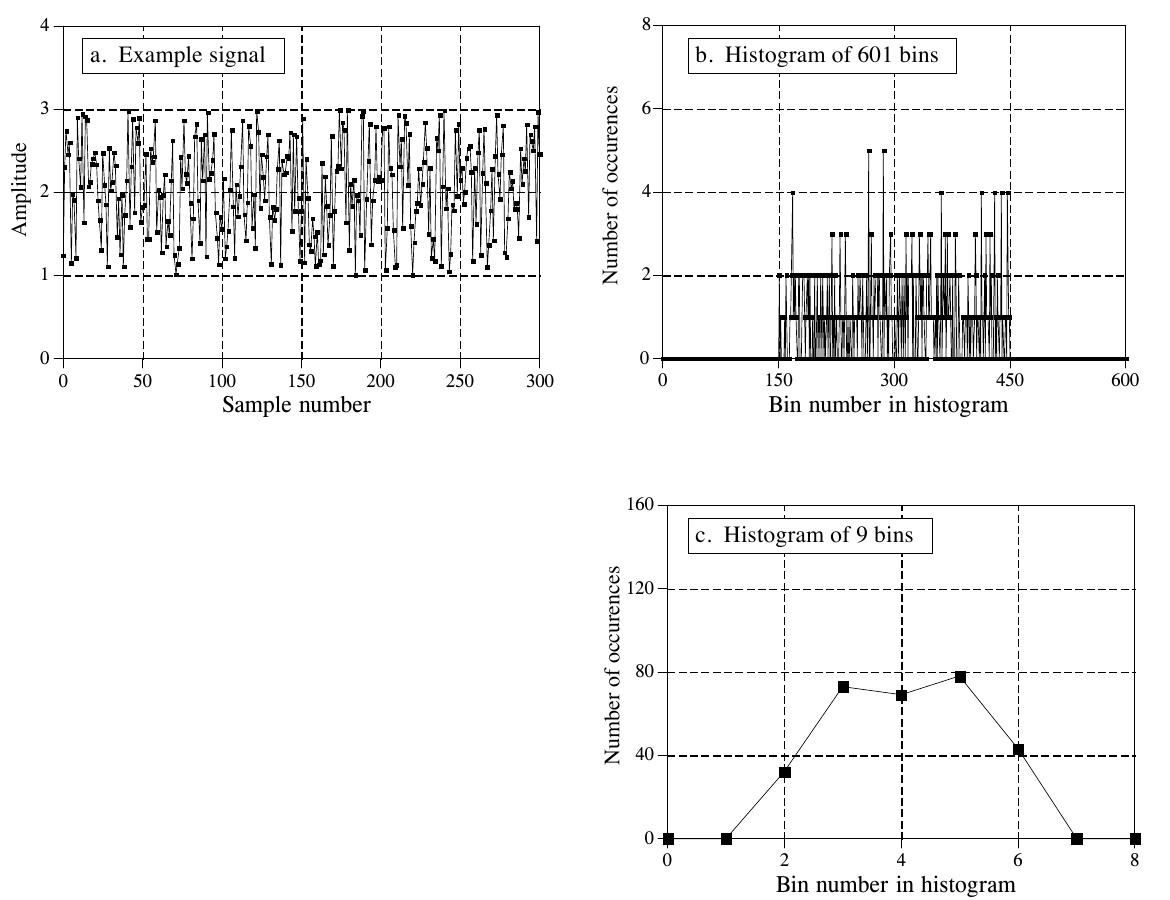
\includegraphics[width=0.975\linewidth,height=0.8\textheight,keepaspectratio]{assets/ch02/fig2-07.png}
\caption*{\textbf{图 2-7　分箱直方图示例。} 如 (a) 所示，本例所用的信号长 300
个采样，每个采样是在 1 到 3 之间均匀分布的浮点数。图 (b) 和 (c) 分别是用
601 个箱和 9
个箱得到的该信号的分箱直方图。可以看到，箱太多会使纵轴方向的分辨率变差，箱太少则使横轴方向的分辨率变差。用更多的采样能让两个方向的分辨率都变好。
（a. Example signal = 示例信号；b. 601 个箱的直方图；c.~9
个箱的直方图。Bin number in histogram = 直方图中的箱号。）}
\end{figure}

该用多少个箱？这是两个问题之间的折中。如图 2-7
所示，箱太多，就难以估计背后 pmf
的高度。这是因为每个箱只落进少数几个采样，统计噪声非常大。另一个极端，箱太少，就难以在水平方向上估计背后的
pmf。换句话说，箱数控制着 y 轴分辨率与 x 轴分辨率之间的权衡。

\section{正态分布}

由随机过程形成的信号，通常有一个钟形的 pdf。这叫正态分布(normal
distribution)、高斯分布(Gauss
distribution)，或简称高斯(Gaussian)，以伟大的德国数学家卡尔·弗里德里希·高斯(Karl
Friedrich Gauss,
1777-1855)命名。这条曲线为什么在自然界中如此常见，稍后结合数字噪声生成来讨论。曲线的基本形状由一个负的平方指数生成：

\[
y(x) = e^{-x^2}
\]

给这条原始曲线加上可调的均值 µ 和标准差
σ，就能变成完整的高斯曲线。此外，还必须对公式做归一化(normalize)，让曲线下的总面积等于
1，这是所有概率分布函数都必须满足的要求。由此得到正态分布的一般形式，它是统计和概率中最重要的关系之一：

\textbf{公式 2-8　正态分布公式，也叫高斯分布，或简称高斯。}
在这个关系式中，P(x) 是概率分布函数，µ 是均值，σ 是标准差。

\[
P(x) = \frac{1}{\sqrt{2\pi}\,\sigma}\, e^{-(x-\mu)^2/2\sigma^2}
\]

图 2-8
给出了几个不同均值和标准差的高斯曲线示例。均值让曲线以某个值为中心，标准差控制钟形的宽度。

\begin{figure}[htbp]
\centering
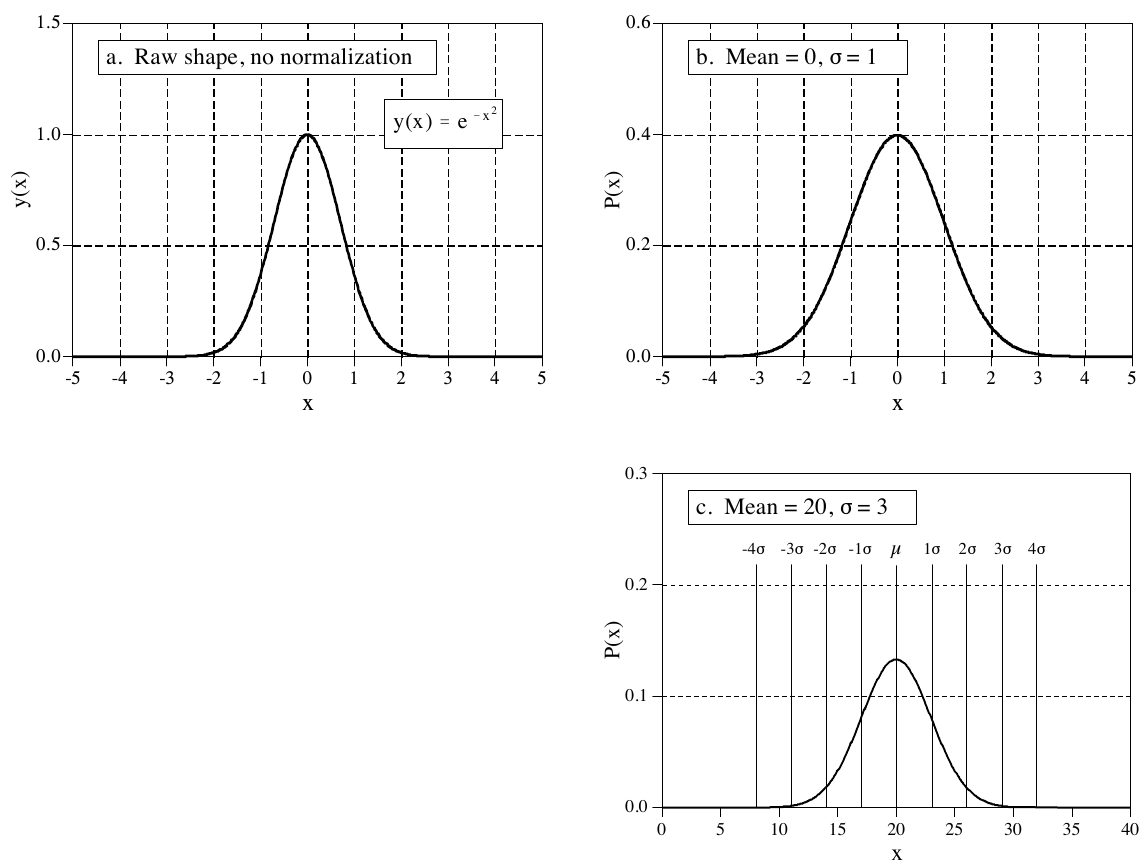
\includegraphics[width=0.954\linewidth,height=0.8\textheight,keepaspectratio]{assets/ch02/fig2-08.png}
\caption*{\textbf{图 2-8　高斯曲线示例。} 图 (a)
是原始曲线的形状，没有归一化，也没有加入可调参数。(b) 和 (c)
展示了不同均值和标准差下的完整高斯曲线。 （a. 原始形状，未归一化(Raw
shape, no normalization)；b. 均值 = 0，σ = 1；c.~均值 = 20，σ =
3，图中竖线标出了 µ 两侧 ±1σ 到 ±4σ 的位置。）}
\end{figure}

高斯曲线有个有趣的特点：它的尾部下降到零的速度非常快，比衰减指数或 1/x
等其他常见函数快得多。例如，在偏离均值 2、4、6
个标准差的地方，高斯曲线的值分别下降到约 1/19、1/7563 和
1/166,666,666。这就是为什么正态分布的信号（如图 2-6c
所示）看起来有一个大致的峰峰值。原则上，这类信号的起伏幅度可以没有上限。但实际上，高斯
pdf
的急剧下降决定了这些极端值几乎永远不会出现。结果是波形看起来比较有界，表观峰峰值大约是
6～8σ。

前面讲过，要求信号落在某个取值范围内的概率，就要对 pdf 积分。pdf
的积分重要到有了自己的名字：累积分布函数(cdf, cumulative distribution
function)。高斯分布有个特别讨厌的问题：它没法用初等方法积分。为了绕开这一点，可以用数值积分(numerical
integration)计算高斯的积分。做法是对连续的高斯曲线做非常密的采样，比如在
−10σ 到 +10σ
之间取几百万个点，然后把这个离散信号的采样累加起来，模拟积分。把这样模拟积分得到的离散曲线存进一张表，用来计算概率。

正态分布的 cdf 如图 2-9 所示，数值列在表 2-5
中。这条曲线在概率中用得非常频繁，所以有自己的符号：Φ(x)（大写希腊字母
phi）。例如，Φ(−2) 的值是
0.0228。这表示在任意随机选取的时刻，信号的值处于 −\dspsym{∞}
到「均值以下两个标准差」之间的概率是 2.28\%。同样，Φ(1) = 0.8413
表示在随机选取的某一时刻，信号的值处于 −\dspsym{∞}
到「均值以上一个标准差」之间的概率是
84.13\%。要计算信号处于两个值之间的概率，需要用 Φ(x)
表中对应的两个数相减。例如，在随机选取的某个时刻，信号的值处于「均值以下两个标准差」与「均值以上一个标准差」之间的概率是：Φ(1)
− Φ(−2) = 0.8185，即 81.85\%。

用这种方法可以算出：正态分布信号的采样，大约 68\% 的时间落在均值 ±1σ
以内，大约 95\% 的时间落在 ±2σ 以内，大约 99.75\% 的时间落在 ±3σ
以内。信号偏离均值超过 10 个标准差的概率小得离谱，从宇宙诞生到现在（约
100 亿年），预计也只会发生几微秒！

\begin{figure}[htbp]
\centering
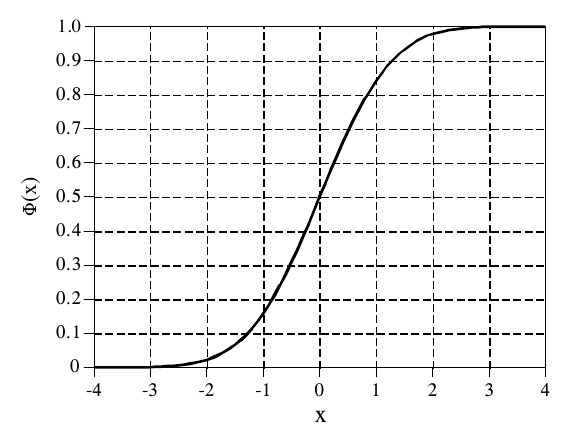
\includegraphics[width=0.471\linewidth,height=0.8\textheight,keepaspectratio]{assets/ch02/fig2-09.png}
\caption*{\textbf{图 2-9 与表 2-5　Φ(x)，正态分布（均值 = 0，标准差 =
1）的累积分布函数。} 这些值是对图 2-8b
所示的正态分布做数值积分算出来的。用文字说，Φ(x)
是正态分布信号在随机选取的某一时刻，其值小于 x 的概率。表中 x
的值以「相对于均值的标准差个数」为单位。}
\end{figure}

{\def\LTcaptype{none} % do not increment counter
\begin{longtable}[]{@{}rrrr@{}}
\toprule\noalign{}
x & Φ(x) & x & Φ(x) \\
\midrule\noalign{}
\endhead
\bottomrule\noalign{}
\endlastfoot
−3.4 & .0003 & 0.0 & .5000 \\
−3.3 & .0005 & 0.1 & .5398 \\
−3.2 & .0007 & 0.2 & .5793 \\
−3.1 & .0010 & 0.3 & .6179 \\
−3.0 & .0013 & 0.4 & .6554 \\
−2.9 & .0019 & 0.5 & .6915 \\
−2.8 & .0026 & 0.6 & .7257 \\
−2.7 & .0035 & 0.7 & .7580 \\
−2.6 & .0047 & 0.8 & .7881 \\
−2.5 & .0062 & 0.9 & .8159 \\
−2.4 & .0082 & 1.0 & .8413 \\
−2.3 & .0107 & 1.1 & .8643 \\
−2.2 & .0139 & 1.2 & .8849 \\
−2.1 & .0179 & 1.3 & .9032 \\
−2.0 & .0228 & 1.4 & .9192 \\
−1.9 & .0287 & 1.5 & .9332 \\
−1.8 & .0359 & 1.6 & .9452 \\
−1.7 & .0446 & 1.7 & .9554 \\
−1.6 & .0548 & 1.8 & .9641 \\
−1.5 & .0668 & 1.9 & .9713 \\
−1.4 & .0808 & 2.0 & .9772 \\
−1.3 & .0968 & 2.1 & .9821 \\
−1.2 & .1151 & 2.2 & .9861 \\
−1.1 & .1357 & 2.3 & .9893 \\
−1.0 & .1587 & 2.4 & .9918 \\
−0.9 & .1841 & 2.5 & .9938 \\
−0.8 & .2119 & 2.6 & .9953 \\
−0.7 & .2420 & 2.7 & .9965 \\
−0.6 & .2743 & 2.8 & .9974 \\
−0.5 & .3085 & 2.9 & .9981 \\
−0.4 & .3446 & 3.0 & .9987 \\
−0.3 & .3821 & 3.1 & .9990 \\
−0.2 & .4207 & 3.2 & .9993 \\
−0.1 & .4602 & 3.3 & .9995 \\
0.0 & .5000 & 3.4 & .9997 \\
\end{longtable}
}

公式 2-8 也可以用来表示正态分布离散信号的概率质量函数。这时 x
只能取信号可能的量化电平之一，比如 12 比特模数转换器输出的 4096
个二进制值之一。忽略 \(1/\sqrt{2\pi}\,\sigma\) 这一项，它只是用来让 pdf
曲线下的总面积等于 1。你要换成能让 pmf 所有值之和等于 1
的那个系数。大多数情况下，做法是先不管归一化，把曲线生成出来，把所有未归一化的值加起来，再把每个值都除以这个总和。

\section{数字噪声的生成}

随机噪声在电子学和 DSP
中都是一个重要话题。例如，它限制了仪器能测到多小的信号、无线电系统能通信多远，以及拍一张
X 光片需要多少辐射剂量。DSP
中一个常见的需求是生成类似各种随机噪声的信号。这是测试那些必须在噪声环境下工作的算法的性能所必需的。

数字噪声生成的核心是随机数生成器(random number
generator)。大多数编程语言都把它作为标准函数。BASIC 语句
\texttt{X\ =\ RND} 每执行一次，就给变量 X
装入一个新的随机数。每个随机数的值都在 0 和 1
之间，落在这两个极端之间任何位置的概率都相等。图 2-10a
是从这种随机数生成器取 128
个采样形成的信号。产生这个信号的背后过程，均值是 0.5，标准差是
\(1/\sqrt{12} = 0.29\)，分布在 0 到 1 之间是均匀的。

算法需要用它在实际运行中会遇到的同类数据来测试。这就需要生成具有高斯 pdf
的数字噪声。用随机数生成器生成这种信号有两种方法。图 2-10
说明了第一种。图 (b) 中每个采样由两个随机数相加得到，即
\texttt{X\ =\ RND+RND}。每个随机数在 0 到 1 之间，所以和在 0 到 2
之间。均值变成 1，标准差变成
\(1/\sqrt{6}\)（记住，独立的随机信号相加时，方差也相加）。如图所示，pdf
从均匀分布变成了三角分布(triangular
distribution)。也就是说，信号更多时间处在 1 附近，处在 0 或 2
附近的时间较少。

图 (c) 把这个思路再推进一步，每个采样由十二个随机数相加得到。均值变成
6，标准差变成 1。最重要的是，pdf
几乎变成了高斯分布。用这个步骤可以生成任意均值和标准差的正态分布噪声信号。对信号中的每个采样：(1)
把十二个随机数相加；(2) 减去 6，使均值为零；(3) 乘以想要的标准差；(4)
加上想要的均值。

这个算法的数学基础是中心极限定理(Central Limit
Theorem)，它是概率论中最重要的概念之一。中心极限定理最简单的表述是：随机数加得越多，它们的和就越接近正态分布。中心极限定理并不要求单个随机数来自某种特定分布，甚至不要求这些随机数来自同一种分布。中心极限定理解释了为什么自然界中如此普遍地见到正态分布的信号：只要有许多不同的随机因素相互作用，得到的
pdf 就会变成高斯分布。

\begin{figure}[htbp]
\centering
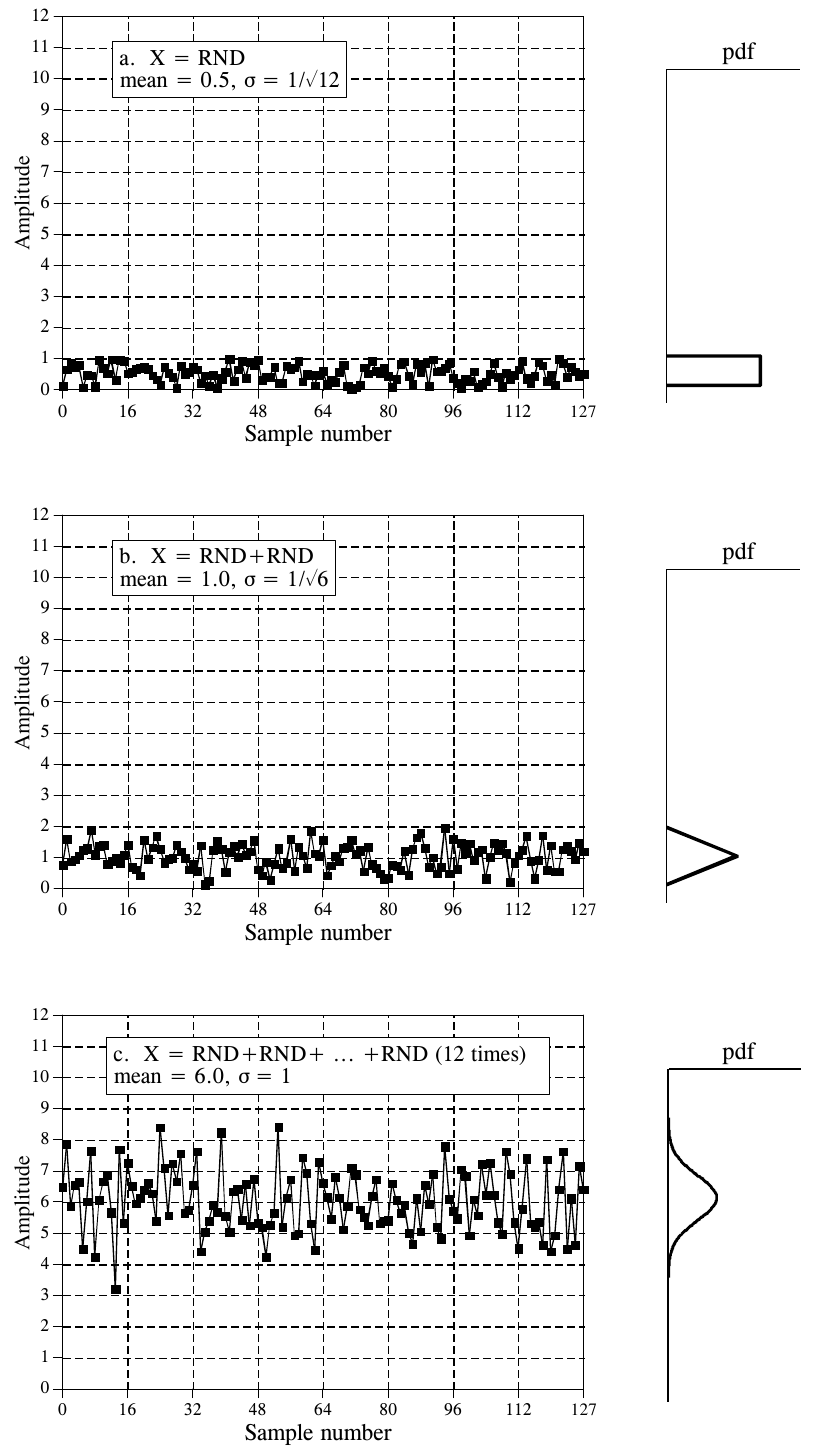
\includegraphics[width=0.679\linewidth,height=0.8\textheight,keepaspectratio]{assets/ch02/fig2-10.png}
\caption*{\textbf{图 2-10　把均匀分布转换成高斯分布。} 图 (a)
的信号中，每个采样都由随机数生成器产生。如 pdf 所示，每个采样的值在 0 到
1 之间均匀分布。(b) 中每个采样由随机数生成器给出的两个值相加而成。(c)
中每个采样由随机数生成器给出的十二个值相加而成。(c) 的 pdf
非常接近高斯分布，均值为 6，标准差为 1。 （a. X = RND，均值 = 0.5，σ =
\(1/\sqrt{12}\)；b. X = RND+RND，均值 = 1.0，σ = \(1/\sqrt{6}\)；c.~X =
RND+RND+\ldots+RND（12 次），均值 = 6.0，σ = 1。右侧小图是各自的 pdf。）}
\end{figure}

生成正态分布随机数的第二种方法，是调用两次随机数生成器，得到 \(R_1\) 和
\(R_2\)。然后就能求出一个正态分布的随机数 X：

\textbf{公式 2-9　生成正态分布的随机数。} \(R_1\) 和 \(R_2\) 是在 0 到 1
之间均匀分布的随机数。由此得到的 X 服从均值为 0、标准差为 1
的正态分布。log 以 e 为底，余弦以弧度为单位。

\[
X = (-2\log R_1)^{1/2}\cos(2\pi R_2)
\]

和前面一样，这种方法也能生成任意均值和标准差的正态分布随机信号：把公式生成的每个数乘以想要的标准差，再加上想要的均值。

随机数生成器从一个种子(seed)开始工作，种子是 0 到 1
之间的一个数。调用随机数生成器时，种子经过一个固定的算法，得到一个 0 到
1
之间的新数。这个新数作为随机数输出，同时在内部保存起来，下次调用时用作种子。把种子变换成新随机数的算法通常是这种形式：

\textbf{公式 2-10　生成 0 到 1 之间均匀分布随机数的常用算法。} 式中 S
是种子，R 是新的随机数，a、b、c 是适当选取的常数。用文字说，就是把 aS+b
除以 c，取余数作为 R。

\[
R = (aS + b) \bmod c
\]

用这种方式，从同一个种子出发可以生成一串连续的随机数。这样程序可以多次运行，每次都使用完全相同的随机数序列。如果你想让随机数序列变化，大多数语言都提供重新设定种子的功能，让你自己选择第一个种子。一种常用的技巧是用时间（系统时钟显示的时间）做种子，这样每次运行程序都会得到新的序列。

从纯数学的角度看，这样生成的数不可能是绝对随机的，因为每个数都完全由前一个数决定。人们常用伪随机(pseudo-random)这个词来描述这种情况。不过你不必担心这一点。随机数生成器生成的序列，在统计意义上随机程度极高。你几乎不可能遇到它们不够用的情况。

\section{精密度与准确度}

精密度(precision)和准确度(accuracy)这两个术语，用来描述进行测量、估计或预测的系统和方法。在所有这些情况下，都有某个你想知道其数值的参数，这叫真值(true
value)，或简称真相(truth)。方法给出一个测量值(measured
value)，你希望它尽可能接近真值。精密度和准确度就是描述这两个值之间可能存在的误差的方式。

遗憾的是，在非技术场合，精密度和准确度经常被混用。事实上，词典给它们下定义时互相引用！尽管如此，科学和工程对两者各有非常明确的定义。你应该注意正确使用这两个术语，别人用错时就默默容忍吧。

举个例子，设想一位海洋学家用声呐系统测量水深。船上发出短促的声脉冲，被海底反射，作为回声在海面被接收。声波在水中的传播速度比较恒定，所以可以根据发射脉冲和接收脉冲之间的时间差求出深度。和所有经验测量一样，测量值和真值之间存在一定的误差。这个测量可能受很多因素影响：电子设备中的随机噪声、海面的波浪、海底的植物生长、水温变化导致声速改变等。

为了研究这些影响，海洋学家在一个已知恰好深 1000
米的地点（真值）连续读取许多次数据。然后把这些测量值整理成图 2-11
所示的直方图。正如中心极限定理所预料的，采集到的数据呈正态分布。均值位于分布的中心，代表根据所有测量数据对深度的最佳估计。标准差决定分布的宽度，描述了连续测量之间有多大的变动。

这就产生了系统可能出现的两类一般误差。第一，均值可能偏离真值，偏离的大小称为测量的准确度。第二，单次测量之间可能不太一致，表现为分布的宽度，这称为测量的精密度，用标准差、信噪比或
CV 来表示。

\begin{figure}[htbp]
\centering
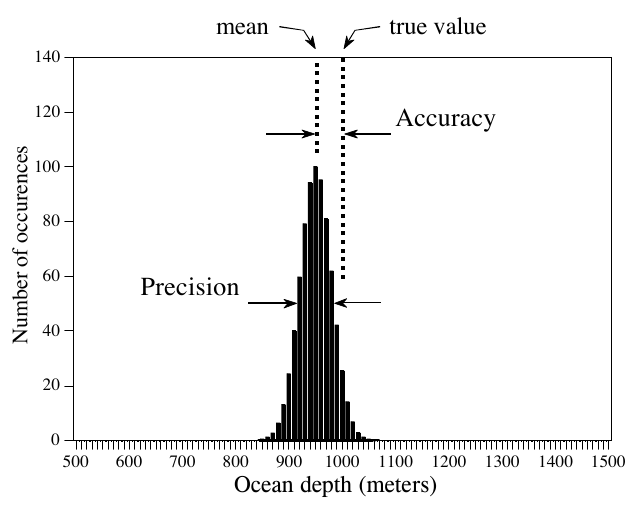
\includegraphics[width=0.529\linewidth,height=0.8\textheight,keepaspectratio]{assets/ch02/fig2-11.png}
\caption*{\textbf{图 2-11　准确度和精密度的定义。}
准确度是真值与产生数据的背后过程的均值之差。精密度是数值的分散程度，用标准差、信噪比或
CV 表示。 （mean = 均值，true value = 真值，Accuracy = 准确度，Precision
= 精密度，Number of occurences = 出现次数，Ocean depth (meters) =
海洋深度（米）。）}
\end{figure}

设想一个准确度好、精密度差的测量：直方图以真值为中心，但非常宽。虽然这些测量作为一个整体是对的，但每一次单独的读数都不能很好地反映真值。这种情况称为重复性(repeatability)差：连续进行的测量彼此不太一致。精密度差源于随机误差(random
errors)，即每次重复测量都会变化的误差。对多次测量取平均，总能改善精密度。简而言之，精密度衡量的是随机噪声。

再设想一个非常精密、但准确度差的测量。这时直方图很窄，但中心不在真值上。连续读数彼此接近，但都有很大的误差。准确度差源于系统误差(systematic
errors)，即每次测量都以完全相同方式重复出现的误差。准确度通常取决于你如何校准(calibrate)系统。例如，在海洋深度测量中，直接测得的参数是时间差，它通过一个把毫秒换算成米的校准过程转换成深度。这个过程可能简单到乘以一个固定速度，也可能复杂到包含几十项二阶修正。对单次测量取平均，对改善准确度毫无帮助。简而言之，准确度衡量的是校准。

实际中，精密度和准确度会以许多方式纠缠在一起。例如，设想用精度 1\%
的电阻搭建一个电子放大器。这个容差表示，在温度、湿度、老化等很宽的条件范围内，每个电阻的阻值都在标称值的
1\%
以内。阻值的这个误差会使放大器的增益产生相应的误差。这个误差是准确度问题还是精密度问题？

答案取决于你怎样进行测量。例如，假设你搭了一个放大器，在几分钟内测试了几次。每次测试增益误差都保持不变，你会得出结论：这是准确度问题。相比之下，假设你搭了一千个这样的放大器，增益会在器件之间随机波动，问题看起来就是精密度问题。同样，其中任何一个放大器的增益都会随温度和其他环境变化而波动，这又会被称为精密度问题。

决定把问题叫做哪一个时，问自己两个问题。第一：对连续读数取平均，能不能得到更好的测量？能，就把这个误差叫精密度；不能，就叫准确度。第二：校准能不能纠正这个误差？能，就叫准确度；不能，就叫精密度。这可能需要好好想一想，尤其要考虑设备将怎样校准、多久校准一次。

% !TEX root = ../main.tex
% 本文件由 build-tex.sh 从 03-DSP指南-第3章中译.md 生成，改内容请改 md 后重新生成

\chapter{ADC 与 DAC}\label{ch-03}

科学和工程中直接遇到的信号，大多是连续的：随距离变化的光强、随时间变化的电压、取决于温度的化学反应速率等。模数转换(ADC,
Analog-to-Digital Conversion)和数模转换(DAC, Digital-to-Analog
Conversion)，就是让数字计算机能和这些日常信号打交道的过程。数字信息和它的连续对应物有两点重要区别：它是采样(sampled)过的，也是量化(quantized)过的。这两点都限制了数字信号能容纳多少信息。本章讲的是信息管理：弄清哪些信息需要保留，哪些信息丢了也无妨。这又进一步决定了在模拟和数字两个世界之间转换时，采样频率、比特数和模拟滤波类型该怎么选。

\section{量化}

先说一点冷知识。你知道，是 digital computer（数字计算机），不是 digit
computer；处理的信息叫 digital data（数字数据），不是 digit
data。那为什么模数转换一般叫 digitize（数字化）和 digitization，而不叫
digitalize 和 digitalization
呢？答案出人意料。等到电子学发明数字技术时，首选的名字早在将近一个世纪前就被医学界抢走了：digitalize
和 digitalization 的意思是给病人服用强心药洋地黄(digitalis)。

图 3-1 展示了一次典型模数转换中的电子波形。图 (a)
是待数字化的模拟信号。如图上的标注所示，这个信号是随时间变化的电压。为了让数字好算，我们假设电压可以在
0 到 4.095 伏之间变化，对应 12 比特数字化器输出的 0 到 4095
之间的数字。注意框图被分成两部分：采样保持(S/H,
sample-and-hold)和模数转换器(ADC)。你在电子学课上可能学过，采样保持的作用是在转换进行期间让进入
ADC
的电压保持不变。不过这里画出它并不是因为这个原因：把数字化拆成这两个阶段，是理解数字化的一个重要理论模型。它恰好长得像常见的电子电路，只是一个幸运的附带好处。

从 (a) 和 (b)
的差别可以看出，采样保持的输出只允许在周期性的时刻改变，在这些时刻，它被设成和输入信号的瞬时值相同。输入信号在两次采样之间发生的变化被完全忽略。也就是说，采样把自变量（本例中是时间）从连续变成离散。

从 (b) 和 (c) 的差别可以看出，ADC 为 (b) 中的每一段平台输出一个 0 到
4095 之间的整数。这就引入了误差，因为每段平台可以是 0 到 4.095
伏之间的任意电压。例如，2.56000 伏和 2.56001 伏都会被转换成数字
2560。换句话说，量化把因变量（本例中是电压）从连续变成离散。

注意我们刻意避免直接比较 (a) 和
(c)，因为那样会把采样和量化混在一起。分开分析它们很重要，因为它们以不同的方式劣化信号，在电子电路中也由不同的参数控制。也有只用其中一个、不用另一个的情况。例如，开关电容滤波器(switched
capacitor filters)就只采样、不量化。

我们先看量化的影响。数字化信号中的任何一个采样，最大误差是 ±½ LSB（LSB
即 Least Significant
Bit，最低有效位，行话里指相邻两个量化电平之间的距离）。图 (d)
是这个例子的量化误差，做适当的换算后用 (c) 减去 (b)
得到。换句话说，数字输出 (c) 等于连续输入 (b) 加上量化误差
(d)。这一分析的一个重要特点是：量化误差看起来非常像随机噪声。

这就引出了量化误差的一个重要模型。大多数情况下，量化的作用无非是给信号加上一定量的随机噪声。这个附加噪声在
±½ LSB 之间均匀分布，均值为零，标准差为 \(1/\sqrt{12}\) LSB（\dspsym{≈}
0.29 LSB）。例如，模拟信号经过 8 比特数字化器，会加上 0.29/256
的均方根噪声，约为满量程值的 1/900。12 比特转换加上的噪声是 0.29/4096
\dspsym{≈} 1/14,000，16 比特转换加上的是 0.29/65536 \dspsym{≈}
1/227,000。既然量化误差是随机噪声，比特数就决定了数据的精密度。例如，你可以这样说：「我们把测量的精密度从
8 比特提高到了 12 比特。」

\begin{figure}[htbp]
\centering
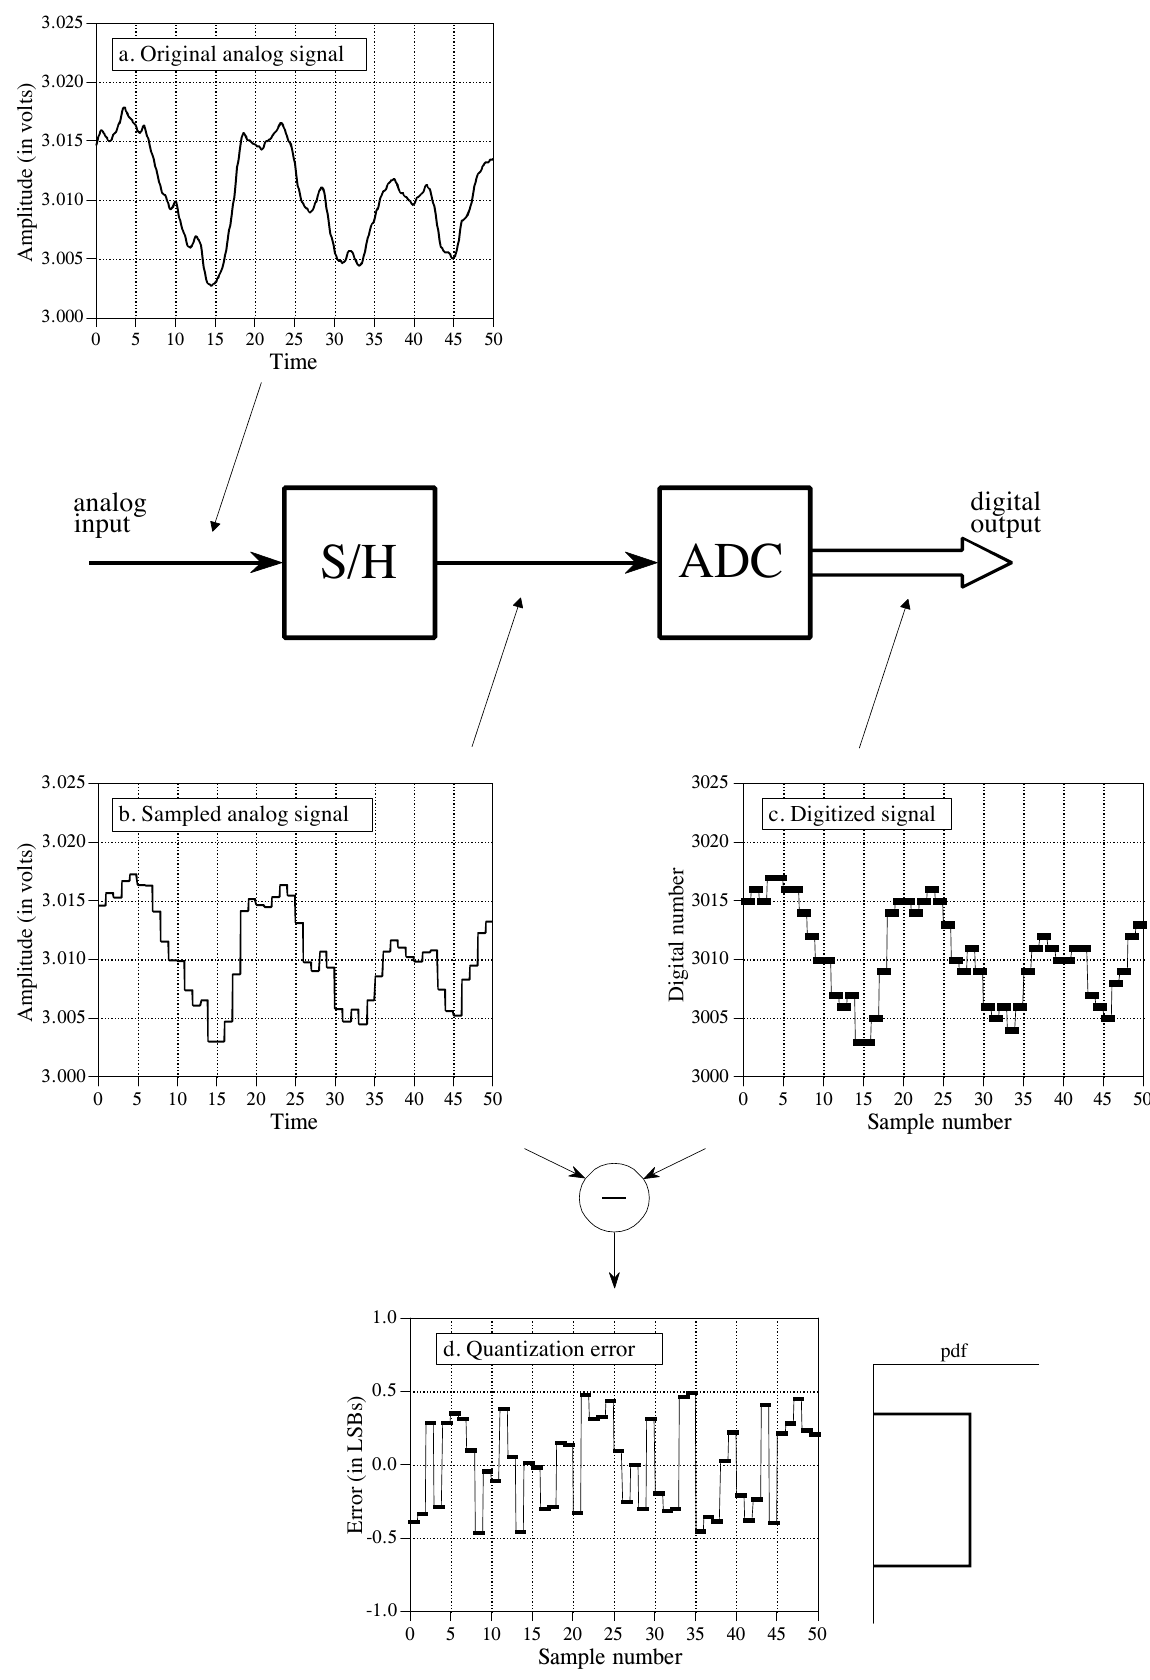
\includegraphics[width=0.958\linewidth,height=0.8\textheight,keepaspectratio]{assets/ch03/fig3-01.png}
\caption*{\textbf{图 3-1　说明数字化过程的波形。}
转换被拆成两个阶段，以便把采样的影响和量化的影响分开。第一阶段是采样保持(S/H)，只保留周期性采样那一刻信号的瞬时值。第二阶段由
ADC 把电压转换成最接近的整数。结果是数字化信号中每个采样都有最多 ±½ LSB
的误差，如 (d) 所示。因此，量化通常可以简单地建模为给信号加上噪声。 （a.
原始模拟信号(Original analog signal)；b. 采样后的模拟信号(Sampled analog
signal)；c.~数字化信号(Digitized signal)；d.~量化误差(Quantization
error)，右侧小图为其 pdf。框图：analog input = 模拟输入，digital output
= 数字输出。Amplitude (in volts) = 幅度（伏），Digital number =
数字值，Error (in LSBs) = 误差（以 LSB 为单位），Time = 时间，Sample
number = 采样序号。）}
\end{figure}

这个模型非常强大，因为量化产生的随机噪声只是简单地叠加到模拟信号中已有的噪声上。例如，设想一个最大幅度为
1.0 伏、随机噪声为 1.0 毫伏均方根值的模拟信号。把它数字化为 8 比特，1.0
伏变成数字 255，1.0 毫伏变成 0.255
LSB。上一章讲过，随机噪声信号叠加时，方差相加。也就是说，信号按平方和(quadrature)的方式相加：\(\sqrt{A^2 + B^2} = C\)。因此数字化信号上的总噪声为
\(\sqrt{0.255^2 + 0.29^2} = 0.386\) LSB，比模拟信号中原有的噪声增加了约
50\%。把同一个信号数字化为 12
比特，噪声几乎不会增加，量化也不会丢失任何东西。在决定一个系统需要多少比特时，问两个问题：(1)
模拟信号中原本已经有多少噪声？(2) 数字信号能容忍多少噪声？

这个量化模型什么时候不成立？只有当量化误差不能当作随机误差处理时。唯一常见的情况是：模拟信号在许多个连续采样中都保持在差不多同一个值，如图
3-2a 所示。即使模拟信号的变化可达 ±½
LSB，输出也会连续许多个采样卡在同一个数字上。这时量化误差不再是附加的随机噪声，而像是一种阈值效应，或者说一种古怪的失真。

抖动(dithering)是改善这类缓变信号数字化的常用技术。如图 3-2b
所示，给模拟信号加上少量随机噪声。本例中，加入的噪声呈正态分布，标准差为
2/3 LSB，峰峰值约为 3 LSB。图 (c)
显示了加入这种抖动噪声后数字化信号的变化。即使原始模拟信号的变化不到 ±½
LSB，加入的噪声也会让数字输出在相邻电平之间随机跳动。

要理解这为什么能改善情况，设想输入信号是恒定的模拟电压 3.0001
伏，正好位于数字电平 3000 和 3001
之间的十分之一处。不加抖动时，对这个信号取 10,000 个采样，会得到 10,000
个相同的数，全都是
3000。接着在加了少量抖动噪声的情况下重做这个思想实验。这 10,000
个值现在会在两个（或更多）电平之间摆动，大约 90\% 是 3000，10\% 是
3001。对全部 10,000 个值取平均，结果接近 3000.1。尽管单次测量有固有的 ±½
LSB
限制，大量采样的统计量却能做得好得多。这真是一种奇怪的情形：加入噪声反而提供了更多信息。

抖动电路可以做得相当精巧，比如用计算机生成随机数，再经过 DAC
产生要加入的噪声。数字化之后，计算机可以用浮点运算从数字信号中减去这些随机数。这种优雅的技术叫减性抖动(subtractive
dither)，但只用在最讲究的系统里。最简单的方法（虽然不一定总能做到）是直接利用模拟信号中已有的噪声来做抖动。

\begin{figure}[htbp]
\centering
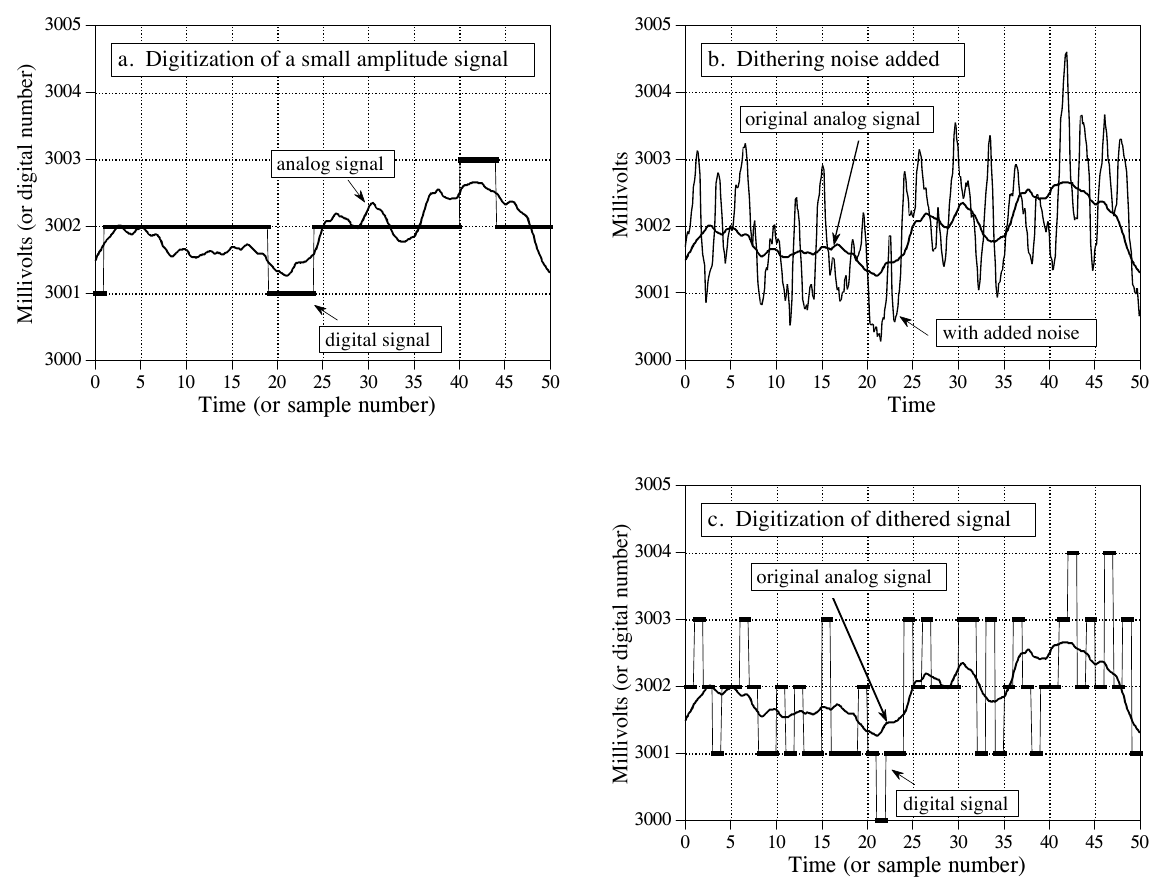
\includegraphics[width=0.958\linewidth,height=0.8\textheight,keepaspectratio]{assets/ch03/fig3-02.png}
\caption*{\textbf{图 3-2　抖动示意。} 图 (a) 显示，变化不到 ±½ LSB
的模拟信号在数字化时会卡在同一个量化电平上。抖动通过给模拟信号加入少量随机噪声来改善这种情况，如
(b) 所示。本例中，加入的噪声呈正态分布，标准差为 2/3 LSB。如 (c)
所示，加入的噪声使数字化信号在相邻量化电平之间跳动，从而提供了关于原始信号的更多信息。
（a. 小幅度信号的数字化(Digitization of a small amplitude signal)；b.
加入抖动噪声(Dithering noise added)；c.~抖动后信号的数字化(Digitization
of dithered signal)。original analog signal = 原始模拟信号，digital
signal = 数字信号，analog signal with added noise =
加了噪声的模拟信号，Millivolts (or digital number) =
毫伏（或数字值），Time (or sample number) = 时间（或采样序号）。）}
\end{figure}

\section{采样定理}

「正确采样」的定义非常简单。假设你以某种方式对一个连续信号做了采样。如果能从这些采样精确地重建出模拟信号，那么你的采样一定是正确的。即使采样数据看起来混乱或不完整，只要这个过程能逆转回去，关键信息就已经被捕获了。

图 3-3 展示了几个正弦波数字化前后的样子。连续的线代表进入 ADC
的模拟信号，方形标记是离开 ADC 的数字信号。在 (a)
中，模拟信号是恒定的直流值，即频率为零的余弦波。由于模拟信号在每两个采样之间都是直线，重建模拟信号所需的全部信息都包含在数字数据中。按照我们的定义，这是正确采样。

\begin{enumerate}
\def\labelenumi{(\alph{enumi})}
\setcounter{enumi}{1}
\tightlist
\item
  中的正弦波频率是采样率的 0.09 倍。比如，它可以代表以每秒 1000
  个采样的速率采样一个每秒 90
  周的正弦波。换一种说法，正弦波每个完整周期里取了 11.1
  个采样。这种情况比上一种复杂，因为不能只在数据点之间画直线来重建模拟信号。这些采样是否正确地代表了模拟信号？答案是肯定的，因为没有任何其他正弦波或正弦波组合会产生这样的采样模式（在下面列出的合理约束条件下）。这些采样只对应一个模拟信号，因此模拟信号可以被精确重建。这又是一个正确采样的例子。
\end{enumerate}

在 (c) 中，把正弦波的频率提高到采样率的 0.31
倍，情况变得更难了。这时每个正弦周期只有 3.2
个采样。采样如此稀疏，甚至看起来都不跟随模拟信号的大致走势。这些采样是否正确地代表了模拟波形？答案仍然是肯定的，理由完全相同：这些采样是模拟信号的唯一表示，重建连续波形所需的全部信息都包含在数字数据中。具体怎么做，本章后面会讨论。显然，这不能只靠在数据点之间画直线，必须更巧妙。尽管看起来很奇怪，按我们的定义，这是正确采样。

在 (d) 中，模拟频率被推到更高的采样率的 0.95 倍，每个正弦周期只有区区
1.05
个采样。这些采样是否正确地代表了数据？不，没有！这些采样代表的是另一个正弦波，而不是模拟信号中的那个。具体来说，原本频率为
0.95 的正弦波，在数字信号中冒充成了频率为 0.05
的正弦波。正弦波在采样过程中改变频率的这种现象叫混叠(aliasing)。就像罪犯可能用化名或假身份（alias）一样，正弦波冒用了一个不属于它的频率。由于数字数据不再唯一对应某个特定的模拟信号，无歧义的重建就不可能了。采样数据中没有任何东西表明原始模拟信号的频率是
0.95 而不是
0.05。正弦波彻底隐藏了自己的真实身份，一桩完美犯罪就此完成！按我们的定义，这是采样不正确的例子。

\begin{figure}[htbp]
\centering
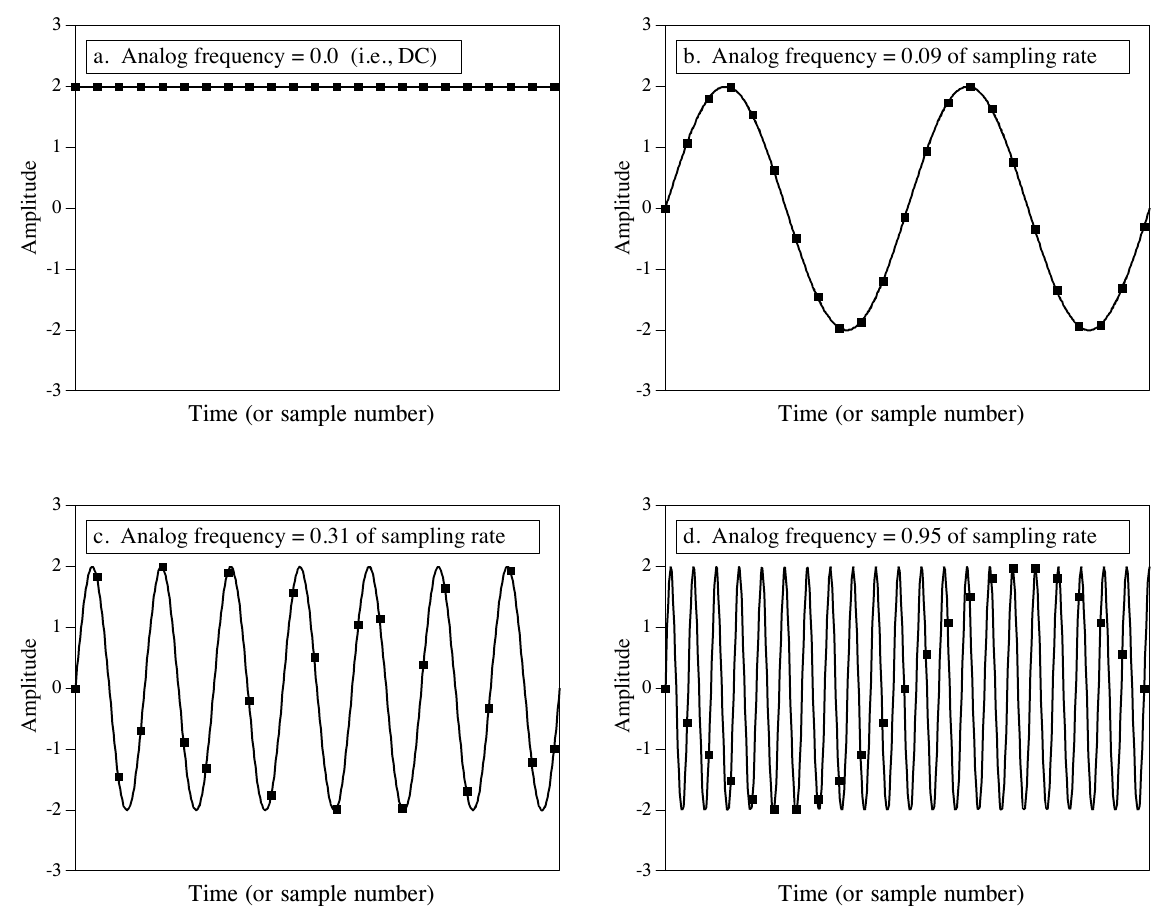
\includegraphics[width=0.967\linewidth,height=0.8\textheight,keepaspectratio]{assets/ch03/fig3-03.png}
\caption*{\textbf{图 3-3　正确采样与不正确采样的示意。}
如果采样包含了重建原始波形所需的全部信息，连续信号的采样就是正确的。图
(a)、(b)、(c) 展示了三个正弦波的正确采样。这一点当然不明显，因为 (c)
中的采样甚至看起来都没抓住波形的形状。尽管如此，这些连续信号中的每一个都和它的采样模式构成唯一的一一对应，这保证了重建可以进行。在
(d)
中，模拟正弦波的频率高于奈奎斯特频率（采样率的一半），导致混叠：采样数据的频率不同于连续信号的频率。由于混叠破坏了信息，原始信号无法从采样中重建。
（a. 模拟频率 = 0.0（即直流）；b. 模拟频率 = 采样率的 0.09
倍；c.~模拟频率 = 采样率的 0.31 倍；d.~模拟频率 = 采样率的 0.95
倍。Amplitude = 幅度，Time (or sample number) = 时间（或采样序号）。）}
\end{figure}

这一推理引出了 DSP 中的一个里程碑：采样定理(sampling
theorem)。它常被称为香农采样定理(Shannon sampling
theorem)或奈奎斯特采样定理(Nyquist sampling theorem)，以 20 世纪 40
年代发表相关论文的作者命名。采样定理指出：只有当连续信号不含高于采样率一半的频率成分时，它才能被正确采样。例如，每秒
2,000 个采样的采样率，要求模拟信号由低于每秒 1000
周的频率组成。如果信号中存在高于这个上限的频率，它们就会被混叠到每秒 0
到 1000 周之间的频率上，和那里原本合法存在的信息混在一起。

讨论采样定理时，有两个术语用得很广：奈奎斯特频率(Nyquist
frequency)和奈奎斯特速率(Nyquist
rate)。遗憾的是，它们的含义并不统一。为了说明这一点，考虑一个由直流到 3
kHz 之间的频率组成的模拟信号。要正确地数字化这个信号，采样率必须达到每秒
6,000 个采样（6 kHz）或更高。假设我们选择以每秒 8,000 个采样（8
kHz）采样，这样直流到 4 kHz
之间的频率都能被正确表示。这时有四个重要的频率：(1) 信号中的最高频率 3
kHz；(2) 它的两倍 6 kHz；(3) 采样率 8 kHz；(4) 采样率的一半 4
kHz。这四个中哪个是奈奎斯特频率，哪个是奈奎斯特速率？看你问谁了！所有可能的组合都有人用。好在大多数作者都会仔细说明自己怎么用这些术语。本书中，两者都指采样率的一半。

图 3-4
展示了混叠过程中频率是怎样改变的。要记住的关键一点是：数字信号不可能包含高于采样率一半（即奈奎斯特频率/速率）的频率。当连续波的频率低于奈奎斯特速率时，采样数据的频率与之相符。但当连续信号的频率高于奈奎斯特速率时，混叠会把这个频率变成采样数据能表示的某个频率。如图
3-4 中的锯齿线所示，高于奈奎斯特速率的每个连续频率，都对应 0
到采样率一半之间的某个数字频率。如果这个较低的频率上恰好已经有一个正弦波，混叠过来的信号就会加到它上面，造成信息损失。混叠是双重诅咒：较高频率和较低频率的信息都可能丢失。假设给你一个包含采样率
0.2
倍频率的数字信号。如果这个信号是正确采样得到的，原始模拟信号的频率一定是
0.2。如果采样时发生了混叠，数字频率 0.2
可能来自模拟信号中无穷多个频率中的任何一个：0.2、0.8、1.2、1.8、2.2、\ldots{}

混叠在采样时能改变频率，也能改变相位(phase)。例如，回头看图 3-3d
中混叠后的信号。混叠后的数字信号相对原始模拟信号是反相的：一个是正弦波，另一个是负的正弦波。换句话说，混叠改变了频率，还引入了
180° 的相移。可能的相移只有两种：0°（无相移）和 180°（反相）。模拟频率在
0 到 0.5、1.0 到 1.5、2.0 到 2.5 等范围内时，相移为零；在 0.5 到
1.0、1.5 到 2.0、2.5 到 3.0 等范围内时，相位反转。

现在我们深入更细致地分析采样以及混叠是怎样发生的。总体目标是理解：信号从连续形式转换成离散形式时，信息发生了什么。问题在于，这两样东西非常不同：一个是连续波形，另一个是一组数。这种「苹果比橘子」的比较让分析变得非常困难。解决办法是引入一个叫冲激串(impulse
train)的理论概念。

图 3-5a 是一个模拟信号的例子。图 (c)
是用冲激串对它采样的结果。冲激串是一个连续信号，由一系列窄尖峰（冲激(impulses)）组成，这些尖峰在采样时刻与原始信号相等。每个冲激都无限窄，这个概念将在第
13
章讨论。在采样时刻之间，波形的值为零。记住，冲激串是一个理论概念，而不是能在电子电路中真实存在的波形。由于原始模拟信号和冲激串都是连续波形，我们就能在两者之间做「苹果比苹果」的比较了。

\begin{figure}[htbp]
\centering
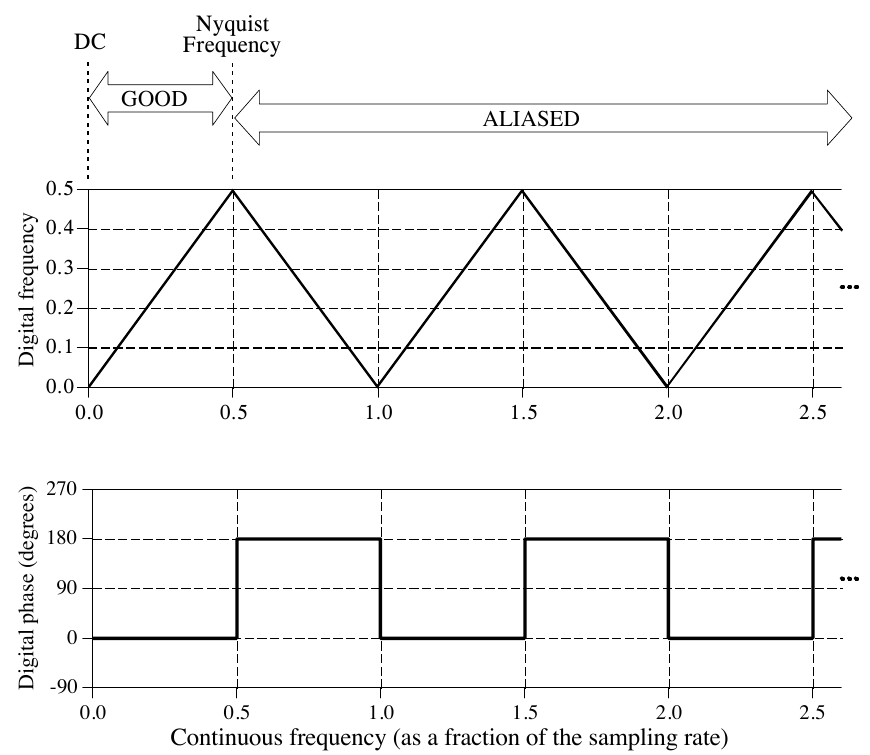
\includegraphics[width=0.725\linewidth,height=0.8\textheight,keepaspectratio]{assets/ch03/fig3-04.png}
\caption*{\textbf{图 3-4　采样时模拟频率到数字频率的转换。}
频率低于采样率一半的连续信号，直接转换成对应的数字频率。高于采样率一半时发生混叠，频率在数字数据中被错误表示。混叠总是把较高的频率变成
0 到 0.5 之间某个较低的频率。此外，混叠还可能把信号的相位改变 180 度。
（上图：Digital frequency = 数字频率，DC = 直流，Nyquist Frequency =
奈奎斯特频率，GOOD = 正确，ALIASED = 混叠。下图：Digital phase (degrees)
= 数字相位（度）。横轴：Continuous frequency (as a fraction of the
sampling rate) = 连续频率（以采样率的倍数表示）。）}
\end{figure}

现在需要研究冲激串和离散信号（一组数）之间的关系。这个很简单：就信息含量而言，两者完全相同。知道其中一个，算出另一个是小事一桩。可以把它们看作横跨模拟世界和数字世界的一座桥的两端。这意味着，只要我们弄懂了把图
3-5a 的波形变成图 3-5c 的波形会带来什么后果，总体目标就达成了。

图 3-5 左栏是三个连续波形，右栏是这些信号对应的频谱(frequency
spectra)。从你的电子学知识来看，这应该是个熟悉的概念：每个波形都可以看作由幅度和频率各异的正弦波组成。后面的章节会详细讨论频域。（等你更熟悉频谱之后，可能想回头再看看这段讨论。）

图 (a) 是我们想要采样的模拟信号。从 (b) 中它的频谱可以看出，它只由 0
到大约 0.33 \(f_s\) 之间的频率成分组成，\(f_s\)
是我们打算使用的采样频率。比如，这可能是一个已滤除了 3.3 kHz
以上所有频率的语音信号。相应地，\(f_s\) 就是 10 kHz（每秒 10,000
个采样），也就是我们打算用的采样率。

用冲激串对 (a) 中的信号采样，得到 (c) 所示的信号，以及 (d)
所示的频谱。这个频谱是原始信号频谱的复制：采样频率的每个整数倍
\(f_s\)、\(2f_s\)、\(3f_s\)、\(4f_s\)
等处，都得到了原始频谱的一份拷贝和一份左右翻转的拷贝。拷贝叫上边带(upper
sideband)，翻转的拷贝叫下边带(lower
sideband)。采样产生了新的频率。这是正确采样吗？答案是肯定的，因为只要去掉
½\(f_s\) 以上的所有频率，(c) 中的信号就能变回 (a)
中的信号。也就是说，一个模拟低通滤波器(low-pass filter)可以把冲激串 (b)
变回原始的模拟信号 (a)。

如果你已经熟悉 DSP
的基础，这里有一个更技术性的解释，说明为什么会出现这种频谱复制。（如果你刚接触
DSP，可以跳过这一段。）在时域中，采样是通过把原始信号乘以一个由单位幅度尖峰组成的冲激串来实现的。这个单位幅度冲激串的频谱，也是一个单位幅度冲激串，尖峰出现在采样频率的整数倍
\(f_s\)、\(2f_s\)、\(3f_s\)、\(4f_s\)
等处。两个时域信号相乘时，它们的频谱做卷积(convolve)。结果是原始频谱被复制到冲激串频谱中每个尖峰的位置上。把原始信号看作同时由正频率和负频率组成，就分别解释了上边带和下边带。这和第
10 章讨论的幅度调制(amplitude modulation)是一回事。

图 (e) 是一个采样不正确的例子，原因是采样率太低。模拟信号仍然包含高达
3.3 kHz 的频率，但采样率降到了 5 kHz。注意横轴上
\(f_s\)、\(2f_s\)、\(3f_s\) \ldots{} 在 (f) 中比在 (d) 中排得更密。频谱
(f) 揭示了问题所在：复制出来的那部分频谱侵入了 0
到采样频率一半之间的频带。虽然 (f)
把这些重叠的频率画得还能分辨，但实际上它们会加在一起，形成一团乱麻。由于没有办法把重叠的频率分开，信息就丢失了，原始信号无法重建。当模拟信号包含高于采样率一半的频率时，就会发生这种重叠。也就是说，我们证明了采样定理。

\begin{figure}[htbp]
\centering
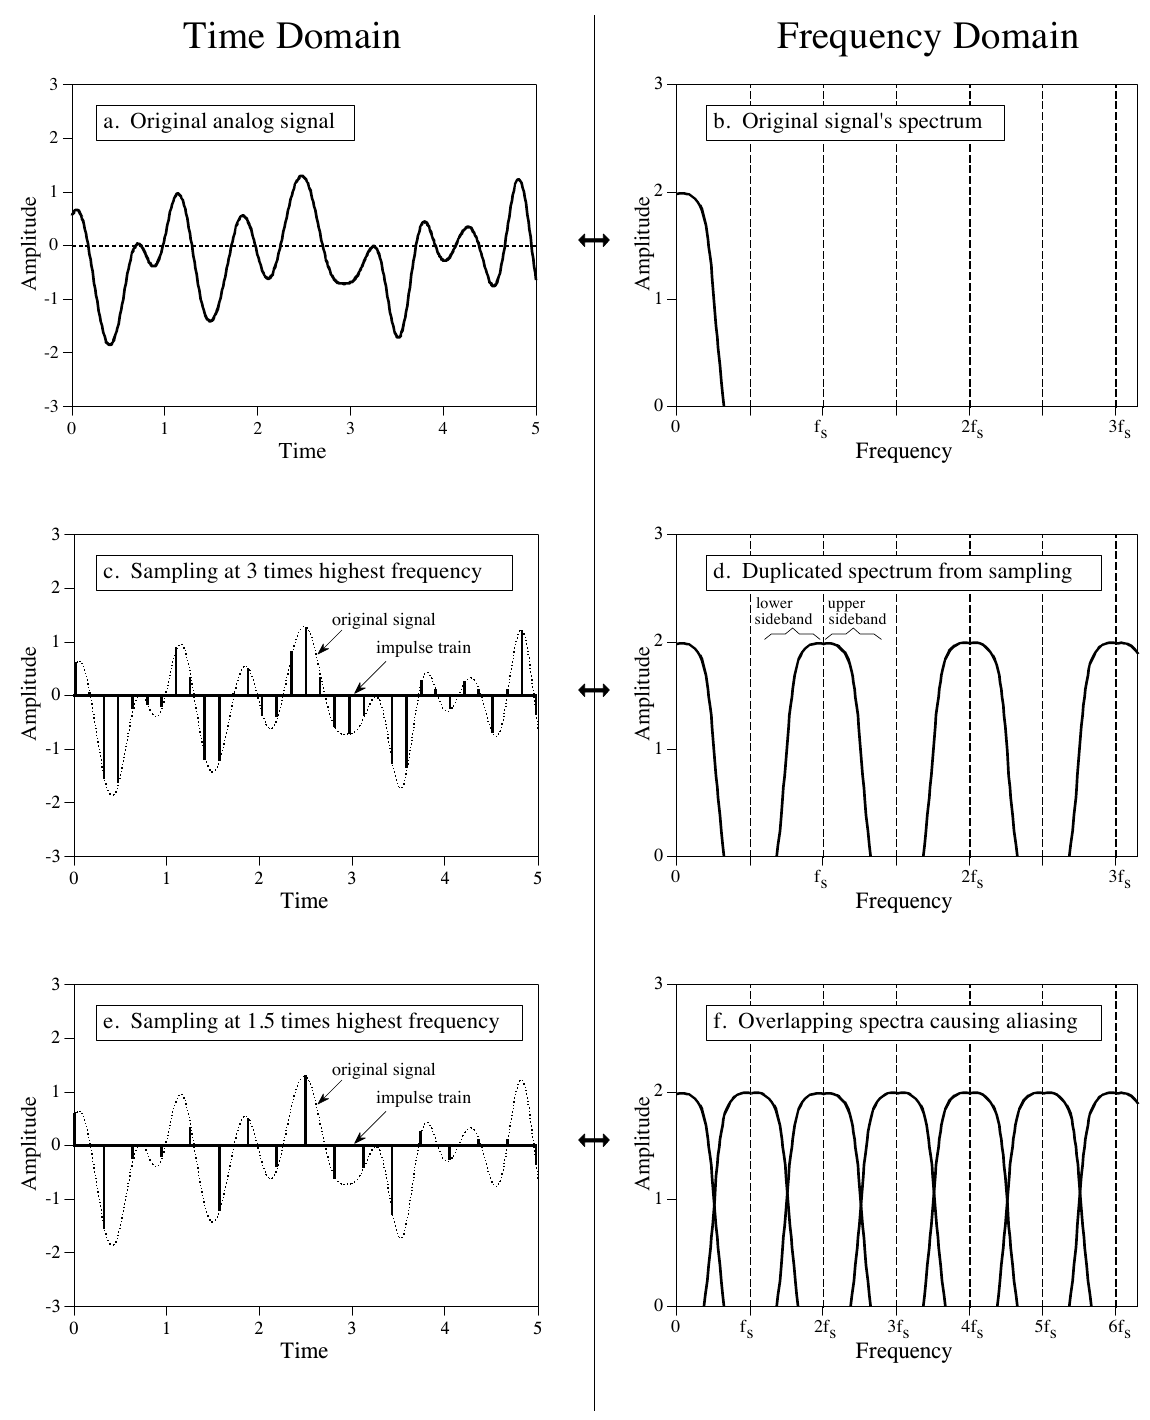
\includegraphics[width=0.958\linewidth,height=0.8\textheight,keepaspectratio]{assets/ch03/fig3-05.png}
\caption*{\textbf{图 3-5　时域和频域中的采样定理。} 图 (a) 和 (b) 是一个由 0 到
0.33 倍采样频率 \(f_s\) 之间的频率成分组成的模拟信号。在 (c)
中，把模拟信号转换成冲激串，以此对它采样。在频域 (d)
中，这使频谱被复制成无穷多个上边带和下边带。由于 (b) 中的原始频率在 (d)
中没有失真地保留着，所以采样是正确的。相比之下，(e)
中的模拟信号（其最高频率）达到采样频率的 0.66
倍，超过了奈奎斯特速率。这导致了混叠，表现为 (f) 中的边带相互重叠。
（左栏 Time Domain = 时域，右栏 Frequency Domain = 频域。a.
原始模拟信号；b. 原始信号的频谱；c.~以最高频率的 3 倍采样（original
signal = 原始信号，impulse train =
冲激串）；d.~采样造成的频谱复制（lower sideband = 下边带，upper sideband
= 上边带）；e. 以最高频率的 1.5 倍采样；f.~频谱重叠导致混叠。Amplitude =
幅度，Time = 时间，Frequency = 频率。）}
\end{figure}

\section{数模转换}

理论上，最简单的数模转换方法是从存储器中取出采样，把它们转换成冲激串。如图
3-6a 所示，对应的频谱见
(b)。正如刚才所说，让这个冲激串通过一个截止频率等于采样率一半的低通滤波器，就能完美地重建原始模拟信号。换句话说，在奈奎斯特频率（采样率的一半）以下，原始信号和冲激串的频谱完全相同。在更高的频率上，冲激串包含这些信息的复制品，而原始模拟信号什么都没有（假设没有发生混叠）。

这种方法虽然在数学上很纯粹，但在电子电路中很难产生所需的窄脉冲。为了绕开这个问题，几乎所有
DAC
都是把上一个值保持住，直到收到下一个采样为止。这叫零阶保持(zeroth-order
hold)，相当于 ADC 中采样保持在 DAC
这一端的对应物。（一阶保持是在点之间连直线，二阶保持用抛物线，依此类推。）零阶保持产生
(c) 中那样的阶梯状外观。

在频域中，零阶保持使冲激串的频谱乘上了 (d) 中那条深色曲线，其公式为：

\textbf{公式 3-1　零阶保持造成的高频幅度衰减。} 这条曲线画在图 3-6d
中。\(f_s\) 表示采样频率。当 f = 0 时，H(f) = 1。

\[
H(f) = \left|\,\frac{\sin(\pi f / f_s)}{\pi f / f_s}\,\right|
\]

它的一般形式是 \(\sin(\pi x)/(\pi x)\)，叫 sinc 函数，记作 sinc(x)。sinc
函数在 DSP
中非常常见，后面的章节会更详细地讨论。如果你已有这方面的背景，可以把零阶保持理解为冲激串与一个宽度等于采样周期的矩形脉冲做卷积。这使频域乘上了矩形脉冲的傅里叶变换(Fourier
transform)，也就是 sinc 函数。在图 (d)
中，浅色线是冲激串的频谱（「正确的」频谱），深色线是
sinc。零阶保持信号的频谱等于这两条曲线的乘积。

用来把零阶保持信号 (c) 转换成重建信号 (f)
的模拟滤波器，需要做两件事：(1) 去掉采样率一半以上的所有频率；(2)
按零阶保持效应的倒数，即
1/sinc(x)，提升各个频率。这相当于在采样频率一半处放大约 36\%。图 (e)
是这个模拟滤波器的理想频率响应。

\begin{figure}[htbp]
\centering
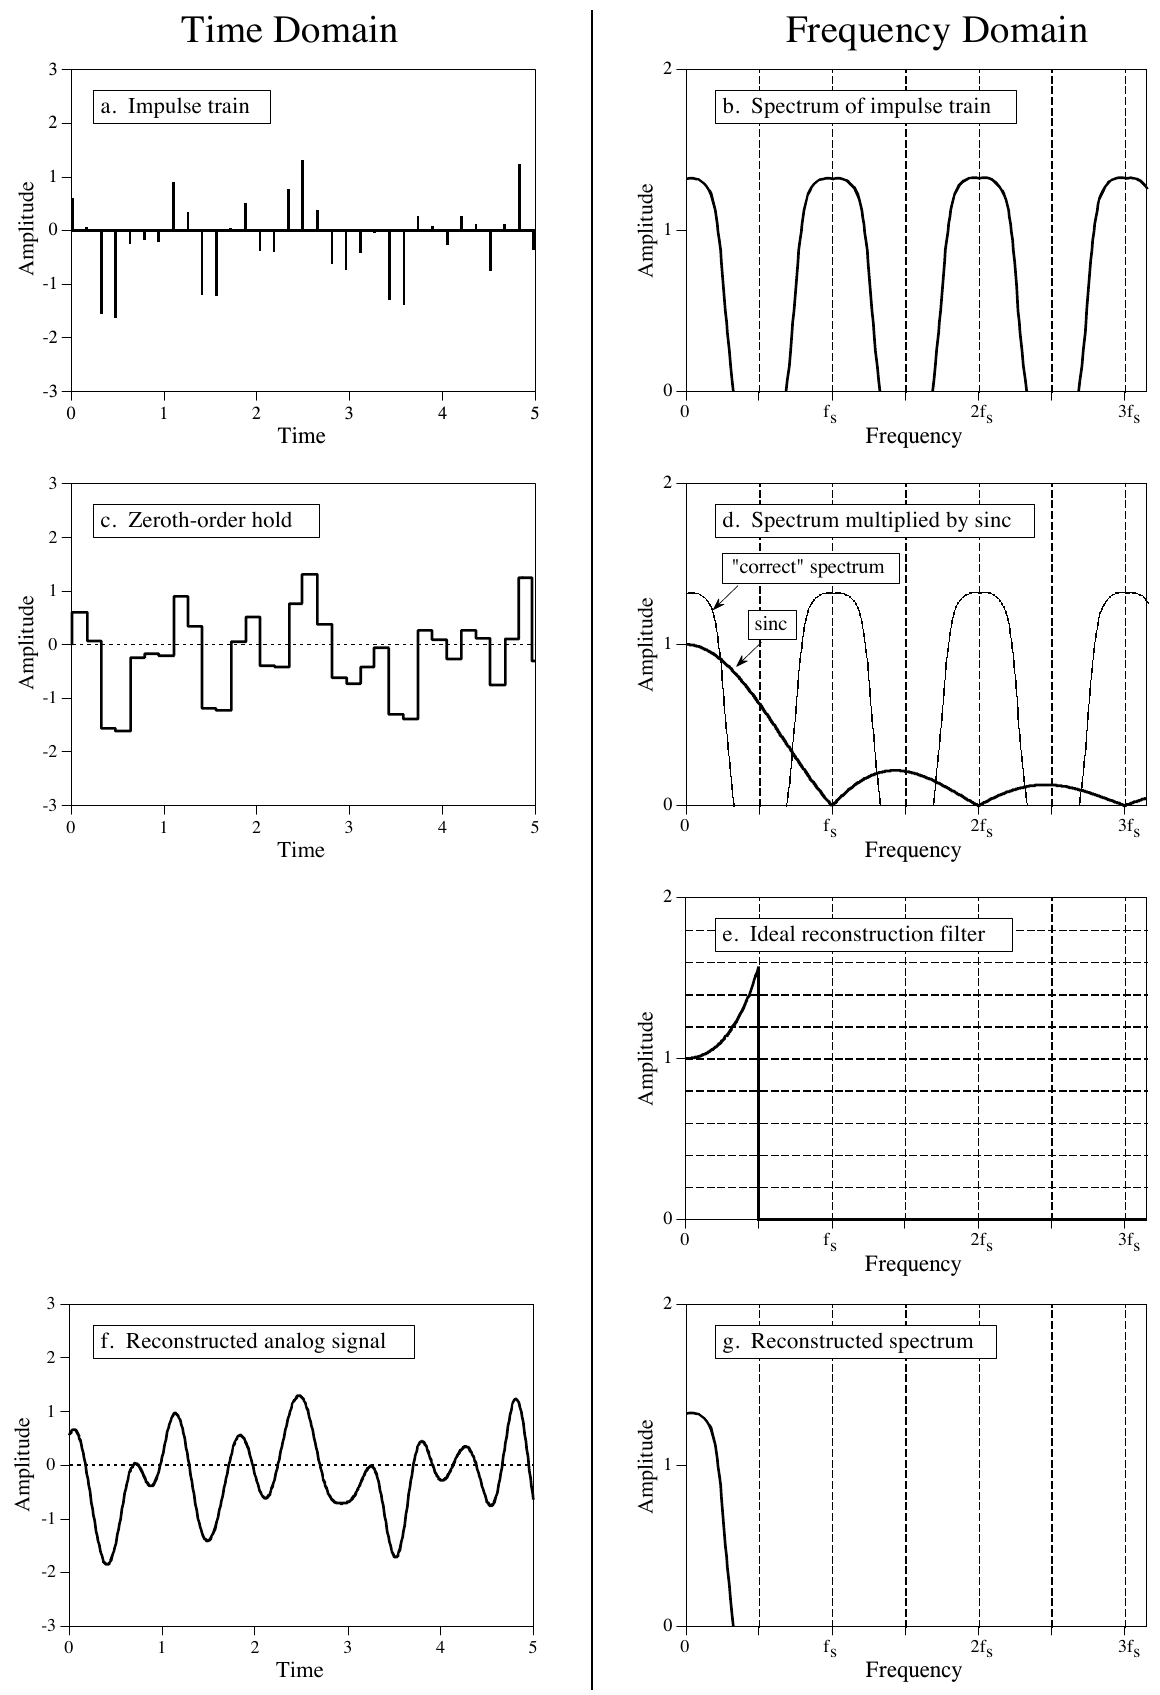
\includegraphics[width=0.967\linewidth,height=0.8\textheight,keepaspectratio]{assets/ch03/fig3-06.png}
\caption*{\textbf{图 3-6　数模转换的分析。} 在 (a)
中，数字数据被转换成冲激串，其频谱见
(b)。用一个电子低通滤波器去掉采样率一半以上的频率，就能把它变成重建信号
(f)［比较 (b) 和 (g)］。然而，大多数电子 DAC 产生的是零阶保持波形
(c)，而不是冲激串。零阶保持的频谱等于冲激串的频谱乘以 (d) 中所示的 sinc
函数。要把零阶保持信号变成重建信号，模拟滤波器必须去掉奈奎斯特速率以上的所有频率，并校正
sinc 的影响，如 (e) 所示。 （a. 冲激串(Impulse train)；b.
冲激串的频谱；c.~零阶保持(Zeroth-order hold)；d.~频谱乘以
sinc（``correct'' spectrum = 「正确的」频谱）；e. 理想重建滤波器(Ideal
reconstruction filter)；f.~重建的模拟信号；g. 重建的频谱。Amplitude =
幅度，Time = 时间，Frequency = 频率。）}
\end{figure}

这种 1/sinc(x) 的频率提升有四种处理方式：(1) 忽略它，接受后果；(2)
设计一个包含 1/sinc(x) 响应的模拟滤波器；(3)
使用本章后面介绍的一种巧妙的多速率(multirate)技术；(4) 在 DAC
之前用软件做校正（见第 24 章）。

在结束关于采样的这一节之前，我们需要破除一个关于模拟信号与数字信号的常见迷思。正如本章所示，数字信号携带的信息量受两方面的限制：第一，每个采样的比特数限制了因变量的分辨率。也就是说，信号幅度的微小变化可能淹没在量化噪声中。第二，采样率限制了自变量的分辨率，即模拟信号中间隔很近的事件可能在两个采样之间丢失。这只是「采样率一半以上的频率会丢失」的另一种说法。

迷思是这样的：「既然模拟信号使用连续的参数，它们在自变量和因变量上都有无限好的分辨率。」不对！模拟信号受到和数字信号同样两个问题的限制：噪声和带宽(bandwidth，信号中允许的最高频率)。模拟信号中的噪声限制了波形幅度的测量，就像数字信号中的量化噪声一样。同样，在模拟信号中分辨间隔很近的事件的能力，取决于波形中允许的最高频率。为了理解这一点，设想一个包含两个间隔很近的脉冲的模拟信号。如果让这个信号通过一个低通滤波器（去掉高频），两个脉冲就会模糊成一团。例如，由直流到
10 kHz 之间的频率构成的模拟信号，和以 20 kHz
采样的数字信号有完全相同的分辨率。必然如此，因为采样定理保证了两者包含相同的信息。

\section{用于数据转换的模拟滤波器}

图 3-7 是采样定理所要求的 DSP
系统框图。输入信号在进入模数转换器之前，先经过一个电子低通滤波器，去掉奈奎斯特频率（采样率的一半）以上的所有频率。这是为了防止采样时发生混叠，因此相应地称为抗混叠滤波器(antialias
filter)。在另一端，数字化信号经过数模转换器和另一个设在奈奎斯特频率的低通滤波器。这个输出滤波器叫重建滤波器(reconstruction
filter)，可能包含前面讲的零阶保持频率提升。遗憾的是，这个简单模型有一个严重问题：电子滤波器的局限，可能和它们试图防止的问题一样糟糕。

\begin{figure}[htbp]
\centering
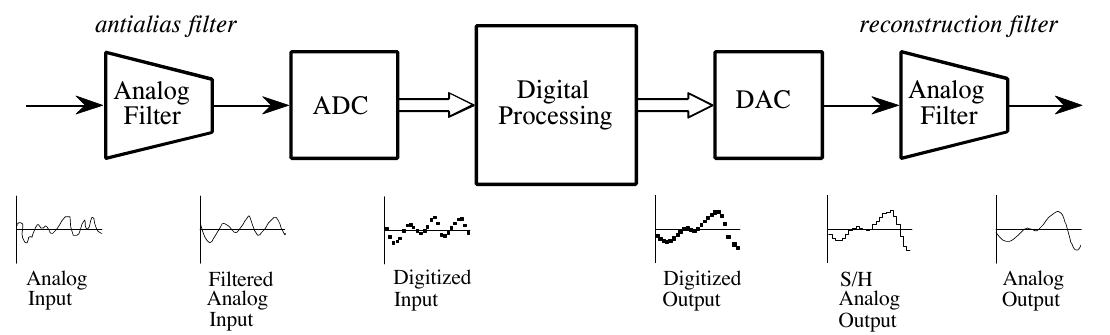
\includegraphics[width=0.925\linewidth,height=0.8\textheight,keepaspectratio]{assets/ch03/fig3-07.png}
\caption*{\textbf{图 3-7　为满足采样定理而使用的模拟电子滤波器。} 放在 ADC
之前的电子滤波器叫抗混叠滤波器，用来去掉采样时会发生混叠的、高于采样率一半的频率成分。放在
DAC
之后的电子滤波器叫重建滤波器，它同样去掉奈奎斯特速率以上的频率，并可能包含对零阶保持的校正。
（antialias filter = 抗混叠滤波器，reconstruction filter =
重建滤波器，Analog Filter = 模拟滤波器，Digital Processing =
数字处理。信号依次为：Analog Input = 模拟输入 \dspsym{→} Filtered Analog
Input = 滤波后的模拟输入 \dspsym{→} Digitized Input = 数字化输入
\dspsym{→} Digitized Output = 数字化输出 \dspsym{→} S/H Analog Output =
采样保持后的模拟输出 \dspsym{→} Analog Output = 模拟输出。）}
\end{figure}

如果你主要关心软件，可能会觉得不需要读这一节。错！即使你发誓永远不碰示波器，理解模拟滤波器的特性对做好
DSP
也很重要。第一，你遇到的每个数字化信号的特性，都取决于采集它时用了哪种抗混叠滤波器。不了解抗混叠滤波器的性质，就无法了解数字信号的性质。第二，DSP
的未来是用软件取代硬件。例如，本章后面介绍的多速率技术，就用巧妙的软件技巧减少了对抗混叠滤波器和重建滤波器的需求。不懂硬件，就没法设计软件来取代它。第三，DSP
的很大一部分和数字滤波器设计有关。常用的策略是从一个等效的模拟滤波器出发，把它转换成软件。后面的章节假定你对模拟滤波器技术有基本的了解。

常用的模拟滤波器有三种：切比雪夫(Chebyshev)、巴特沃斯(Butterworth)和贝塞尔(Bessel，也叫汤普森(Thompson)滤波器)。每一种都是为优化某一项不同的性能参数而设计的。每种滤波器的复杂度都可以通过选择极点(poles)和零点(zeros)的个数来调节，这两个数学术语后面的章节会讨论。滤波器的极点越多，需要的电子元件就越多，性能也越好。这些名字描述的是滤波器的作用，而不是电阻和电容的某种特定排列。例如，一个
6 极点贝塞尔滤波器可以用许多不同类型的电路实现，它们的整体特性都相同。就
DSP
而言，这些滤波器的特性比它们怎样搭建更重要。尽管如此，我们还是先简短介绍一下这些滤波器的电子设计，以提供一个整体框架。

图 3-8 是模拟滤波器设计中的一个常用基本单元：改进型 Sallen-Key
电路(modified Sallen-Key circuit)，以 20 世纪 50
年代描述这一技术的论文作者命名。图中所示的电路是一个 2
极点低通滤波器，可以配置成三种基本类型中的任意一种。表 3-1
提供了选择合适电阻和电容所需的信息。例如，要设计一个 1 kHz、2
极点的巴特沃斯滤波器，表 3-1 给出参数：k1 = 0.1592，k2 = 0.586。随意选取
R1 = 10K 和 C = 0.01 µF（运放电路的常用值），就能算出 R 和 Rf 分别为
15.95K 和 5.86K。把后两个值取整到最接近的 1\% 标准电阻，得到 R =
15.8K，Rf = 5.90K。所有元件的精度都应在 1\% 或更好。

\begin{figure}[htbp]
\centering
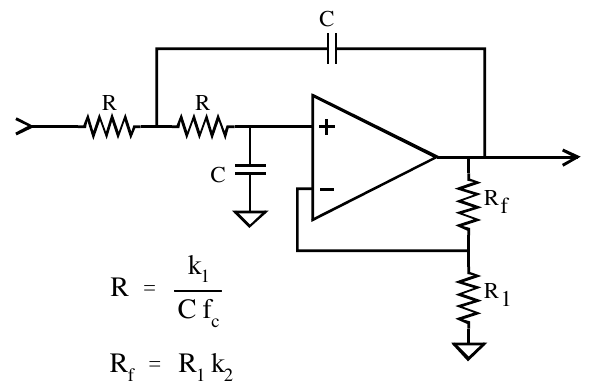
\includegraphics[width=0.496\linewidth,height=0.8\textheight,keepaspectratio]{assets/ch03/fig3-08.png}
\caption*{\textbf{图 3-8　改进型 Sallen-Key 电路，有源滤波器设计的基本单元。}
图示电路实现一个 2
极点低通滤波器。级联多级可以构成更高阶（更多极点）的滤波器。从表 3-1
查出 k1 和 k2，随意选取 R1 和 C（可以试试 10K 和 0.01
µF），再用图中的公式算出 R 和 Rf。参数 \(f_c\)
是滤波器的截止频率，单位为赫兹。}
\end{figure}

图中的两个公式：

\[
R = \frac{k_1}{C\,f_c}, \qquad R_f = R_1\,k_2
\]

\textbf{表 3-1　设计贝塞尔、巴特沃斯和切比雪夫（6\%
纹波）滤波器的参数。}

\begingroup\scriptsize\setlength{\tabcolsep}{3pt}

{\def\LTcaptype{none} % do not increment counter
\begin{longtable}[]{@{}
  >{\raggedright\arraybackslash}p{(\linewidth - 14\tabcolsep) * \real{0.1000}}
  >{\raggedright\arraybackslash}p{(\linewidth - 14\tabcolsep) * \real{0.1000}}
  >{\raggedleft\arraybackslash}p{(\linewidth - 14\tabcolsep) * \real{0.1333}}
  >{\raggedleft\arraybackslash}p{(\linewidth - 14\tabcolsep) * \real{0.1333}}
  >{\raggedleft\arraybackslash}p{(\linewidth - 14\tabcolsep) * \real{0.1333}}
  >{\raggedleft\arraybackslash}p{(\linewidth - 14\tabcolsep) * \real{0.1333}}
  >{\raggedleft\arraybackslash}p{(\linewidth - 14\tabcolsep) * \real{0.1333}}
  >{\raggedleft\arraybackslash}p{(\linewidth - 14\tabcolsep) * \real{0.1333}}@{}}
\toprule\noalign{}
\begin{minipage}[b]{\linewidth}\raggedright
极点数
\end{minipage} & \begin{minipage}[b]{\linewidth}\raggedright
级
\end{minipage} & \begin{minipage}[b]{\linewidth}\raggedleft
贝塞尔 k1
\end{minipage} & \begin{minipage}[b]{\linewidth}\raggedleft
贝塞尔 k2
\end{minipage} & \begin{minipage}[b]{\linewidth}\raggedleft
巴特沃斯 k1
\end{minipage} & \begin{minipage}[b]{\linewidth}\raggedleft
巴特沃斯 k2
\end{minipage} & \begin{minipage}[b]{\linewidth}\raggedleft
切比雪夫 k1
\end{minipage} & \begin{minipage}[b]{\linewidth}\raggedleft
切比雪夫 k2
\end{minipage} \\
\midrule\noalign{}
\endhead
\bottomrule\noalign{}
\endlastfoot
2 & 第 1 级 & 0.1251 & 0.268 & 0.1592 & 0.586 & 0.1293 & 0.842 \\
4 & 第 1 级 & 0.1111 & 0.084 & 0.1592 & 0.152 & 0.2666 & 0.582 \\
& 第 2 级 & 0.0991 & 0.759 & 0.1592 & 1.235 & 0.1544 & 1.660 \\
6 & 第 1 级 & 0.0990 & 0.040 & 0.1592 & 0.068 & 0.4019 & 0.537 \\
& 第 2 级 & 0.0941 & 0.364 & 0.1592 & 0.586 & 0.2072 & 1.448 \\
& 第 3 级 & 0.0834 & 1.023 & 0.1592 & 1.483 & 0.1574 & 1.846 \\
8 & 第 1 级 & 0.0894 & 0.024 & 0.1592 & 0.038 & 0.5359 & 0.522 \\
& 第 2 级 & 0.0867 & 0.213 & 0.1592 & 0.337 & 0.2657 & 1.379 \\
& 第 3 级 & 0.0814 & 0.593 & 0.1592 & 0.889 & 0.1848 & 1.711 \\
& 第 4 级 & 0.0726 & 1.184 & 0.1592 & 1.610 & 0.1582 & 1.913 \\
\end{longtable}
}

\endgroup

所用的具体运放(op
amp)型号并不关键，只要它的单位增益频率比滤波器的截止频率高 30 到 100
倍以上即可。只要滤波器的截止频率低于约 100 kHz，这个要求很容易满足。

4、6、8 极点的滤波器，分别由 2、3、4
个这样的电路级联(cascade)而成。例如，图 3-9 是一个 6
极点贝塞尔滤波器的原理图，它由表 3-1 中的三级构成。每一级的 k1 和 k2
参数都不同，R 和 Rf 也随之不同。

\begin{figure}[htbp]
\centering
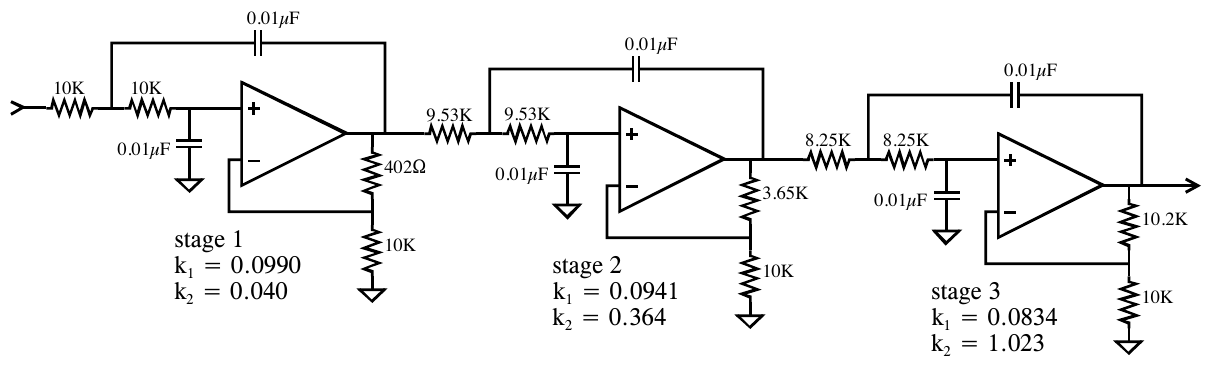
\includegraphics[width=1.000\linewidth,height=0.8\textheight,keepaspectratio]{assets/ch03/fig3-09.png}
\caption*{\textbf{图 3-9　由三个 Sallen-Key 电路级联构成的 6 极点贝塞尔滤波器。}
这是一个截止频率为 1 kHz 的低通滤波器。 （stage 1/2/3 = 第 1/2/3
级，各级标出了所用的 k1、k2。）}
\end{figure}

需要高通滤波器(high-pass filter)？只要把电路中的 R 和 C 元件对调即可（Rf
和 R1 保持不动）。

这类电路在小批量制造和研发应用中非常常见；但真正的量产要求把滤波器做成集成电路(integrated
circuit)。问题在于，直接在硅片上做电阻很难。答案是开关电容滤波器。图
3-10 把它和一个简单的 RC
网络作比较，以说明它的工作原理。如果把阶跃函数(step function)送入 RC
低通滤波器，输出会按指数规律上升，直到与输入相等。电容上的电压不会瞬间改变，因为电阻限制了电荷的流动。

开关电容滤波器的做法，是用两个电容和一个电子开关取代基本的电阻-电容网络。新加入的电容比原有的电容小得多，比如只有它的
1\%。开关以很高的频率（通常比滤波器的截止频率快 100
倍）交替地把小电容接到输入端和输出端。开关接到输入端时，小电容迅速充电到输入端当前的电压。开关接到输出端时，小电容上的电荷转移到大电容上。在电阻中，电荷转移的速率由阻值决定；在开关电容电路中，电荷转移的速率由小电容的容值和开关频率决定。这带来了开关电容滤波器一个非常有用的特性：滤波器的截止频率与驱动开关的时钟频率成正比。这使开关电容滤波器非常适合以多种采样率工作的数据采集系统。这些器件很好用：花十块钱，就能在一个
8 引脚的集成电路里得到 8 极点滤波器的性能。

\begin{figure}[htbp]
\centering
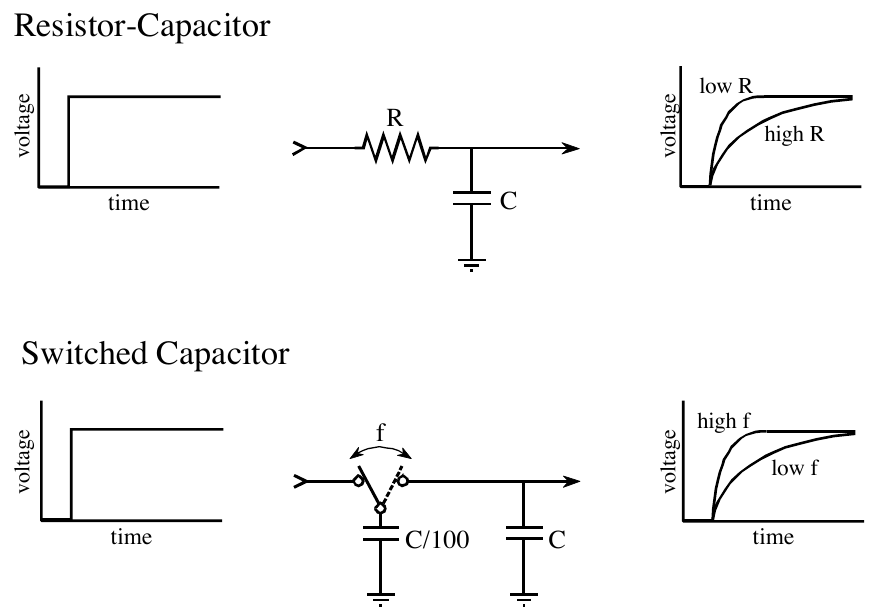
\includegraphics[width=0.733\linewidth,height=0.8\textheight,keepaspectratio]{assets/ch03/fig3-10.png}
\caption*{\textbf{图 3-10　开关电容滤波器的工作原理。}
开关电容滤波器用开关和电容来模拟电阻。如等效的阶跃响应所示，两个电容加一个开关可以起到和电阻-电容网络相同的作用。
（上：Resistor-Capacitor = 电阻-电容网络，low R / high R =
小电阻/大电阻；下：Switched Capacitor = 开关电容，high f / low f =
高/低开关频率，小电容为 C/100。voltage = 电压，time = 时间。）}
\end{figure}

现在讲重点：三种经典滤波器的特性。我们要考察的第一个性能参数是截止的陡峭程度。低通滤波器的设计目标是阻断截止频率以上的所有频率（阻带(stopband)），同时让截止频率以下的所有频率通过（通带(passband)）。图
3-11
以对数（dB）刻度展示了这三种滤波器的频率响应。图中的滤波器截止频率都是 1
赫兹，但可以直接按比例换算到你需要的任何截止频率。这些滤波器表现如何？切比雪夫显然最好，巴特沃斯差一些，贝塞尔简直糟透了！你大概已经猜到了，这正是切比雪夫的设计目标：尽可能快地滚降(roll-off，幅度下降)。

遗憾的是，即使是 8
极点切比雪夫滤波器，用作抗混叠滤波器也不如你希望的那样好。例如，设想一个以每秒
10,000 个采样采样的 12 比特系统。采样定理规定，5 kHz
以上的任何频率都会发生混叠，这是你想避免的。稍加估算，你决定 5 kHz
以上的所有频率在幅度上都必须衰减到
1/100，以保证任何混叠频率的幅度都小于百分之一。查看图
3-11c，你会发现截止频率为 1 赫兹的 8 极点切比雪夫滤波器，要到大约 1.35
赫兹才能达到 100
倍的衰减(attenuation，信号减小)。换算到这个例子，滤波器的截止频率必须设在
3.7 kHz，才能让 5 kHz 以上的一切都达到所需的衰减。这导致 3.7 kHz 到 5
kHz 之间的频带浪费在模拟滤波器不够陡的滚降上。

一个微妙之处：尽管 12 比特有 4096 级，本例中 100
倍的衰减很可能也够了。由图 3-4，5100 赫兹会混叠到 4900 赫兹，6000
赫兹会混叠到 4000 赫兹，依此类推。你并不在乎 5000 到 6300
赫兹之间信号的幅度，因为它们混叠到的是 3700 到 5000
赫兹之间那段不可用的区域。一个频率要混叠进滤波器的通带（0 到 3.7
kHz），它必须高于 6300 赫兹，即 3700 赫兹截止频率的 1.7 倍。如图 3-11c
所示，8 极点切比雪夫滤波器在截止频率 1.7 倍处的衰减约为
1300，比我们分析开始时设定的 100
充裕得多。这个故事的寓意是：在大多数系统中，大约 0.4 到 0.5
倍采样频率之间的频带，是一片充斥着滤波器滚降和混叠信号的不可用荒地。这是模拟滤波器局限的直接结果。

完美低通滤波器的频率响应在整个通带内是平坦的。在图 3-11
中，所有滤波器在这方面看起来都很好，但这只是因为纵轴用的是对数刻度。把图换成线性纵轴刻度，情况就不一样了，如图
3-12 所示。这时就能看到切比雪夫滤波器的通带纹波(passband
ripple，通过频率的幅度呈波浪状变化)。事实上，切比雪夫滤波器正是靠允许这种通带纹波，才获得了出色的滚降。滤波器允许的通带纹波越大，滚降就能越快。用表
3-1 设计的所有切比雪夫滤波器，通带纹波都约为 6\%（0.5
dB），这是一个不错的折中，也是常见的选择。一种类似的设计------椭圆滤波器(elliptic
filter)------在通带和阻带中都允许纹波。椭圆滤波器虽然更难设计，但能在滚降和通带纹波之间取得更好的平衡。

\begin{figure}[htbp]
\centering
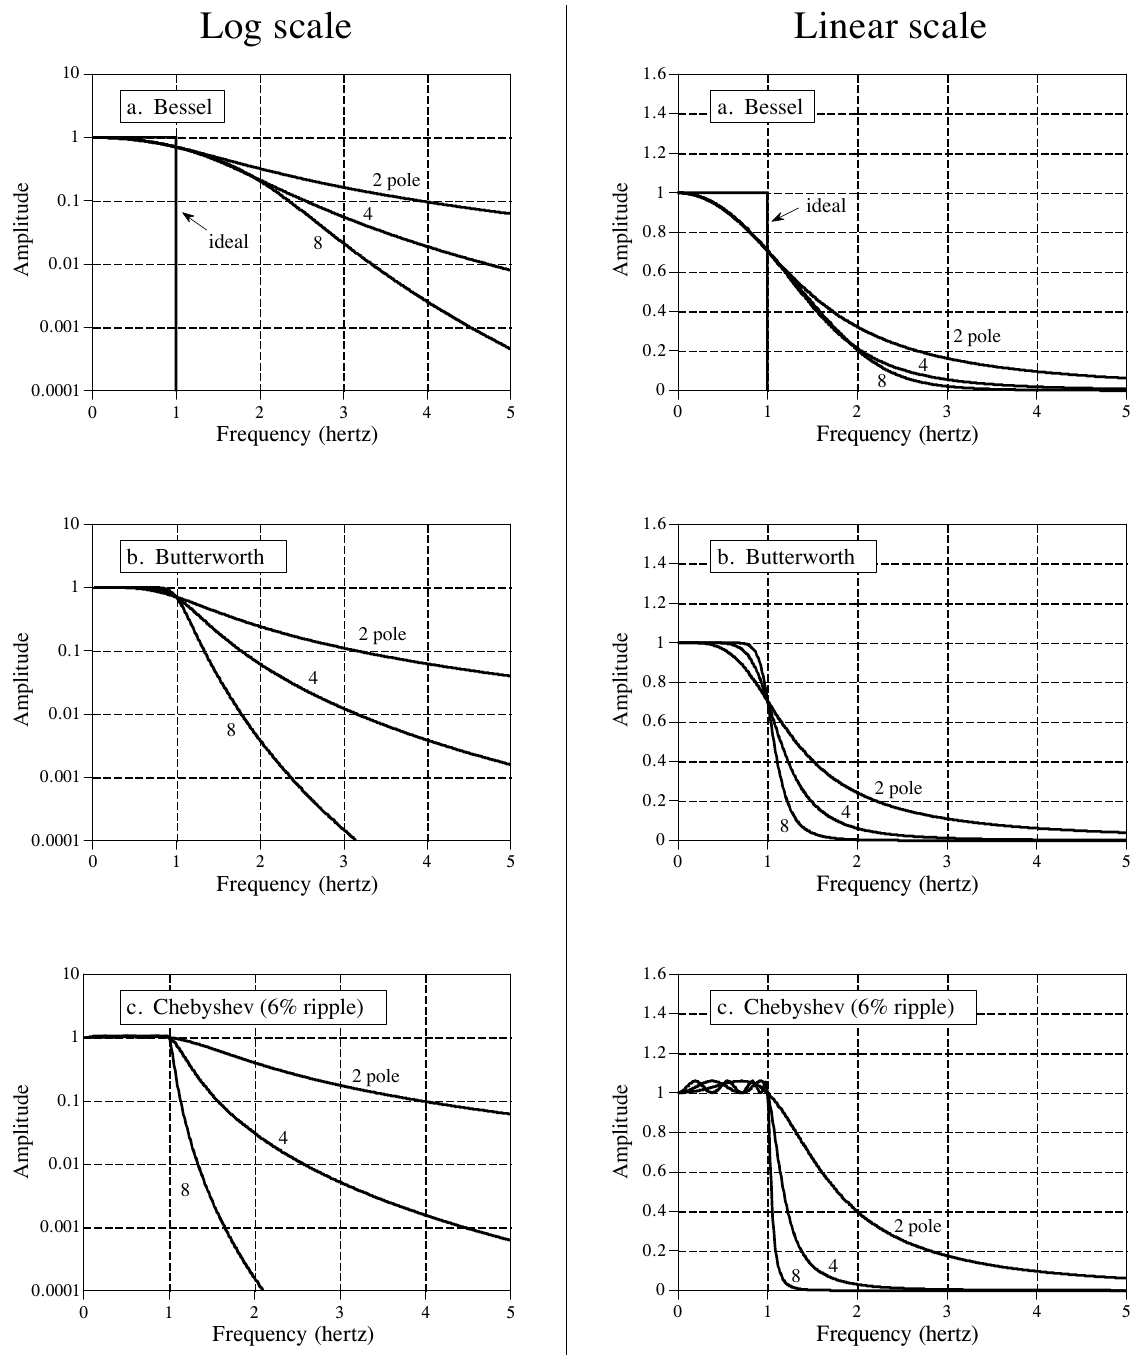
\includegraphics[width=0.950\linewidth,height=0.8\textheight,keepaspectratio]{assets/ch03/fig3-11-12.png}
\caption*{\textbf{图 3-11（左栏）　三种滤波器在对数刻度上的频率响应。}
切比雪夫滤波器的滚降最陡。}
\end{figure}

\textbf{图 3-12（右栏）　三种滤波器在线性刻度上的频率响应。}
巴特沃斯滤波器的通带最平坦。 （Log scale = 对数刻度，Linear scale =
线性刻度。a. 贝塞尔；b. 巴特沃斯；c.~切比雪夫（6\% 纹波）。曲线旁的 2
pole / 4 / 8 = 2/4/8 极点，ideal = 理想响应。Amplitude = 幅度，Frequency
(hertz) = 频率（赫兹）。）

相比之下，巴特沃斯滤波器的优化目标是在通带内不允许纹波的前提下，提供尽可能陡的滚降。它常被称为最大平坦(maximally
flat)滤波器，等同于通带纹波设计为零的切比雪夫滤波器。贝塞尔滤波器在通带内没有纹波，但滚降比巴特沃斯差得多。

最后一个要评估的参数是阶跃响应(step
response)，即输入从一个值迅速变到另一个值时滤波器的反应。图 3-13
是三种滤波器各自的阶跃响应。横轴对应截止频率为 1
赫兹的滤波器，对于更高的截止频率，可以（按反比）换算。例如，截止频率为
1000
赫兹时，阶跃响应的时间单位就是毫秒而不是秒。巴特沃斯和切比雪夫滤波器会出现过冲(overshoot)和振铃(ringing，幅度慢慢衰减的振荡)。相比之下，贝塞尔滤波器没有这两个讨厌的问题。

\begin{figure}[htbp]
\centering
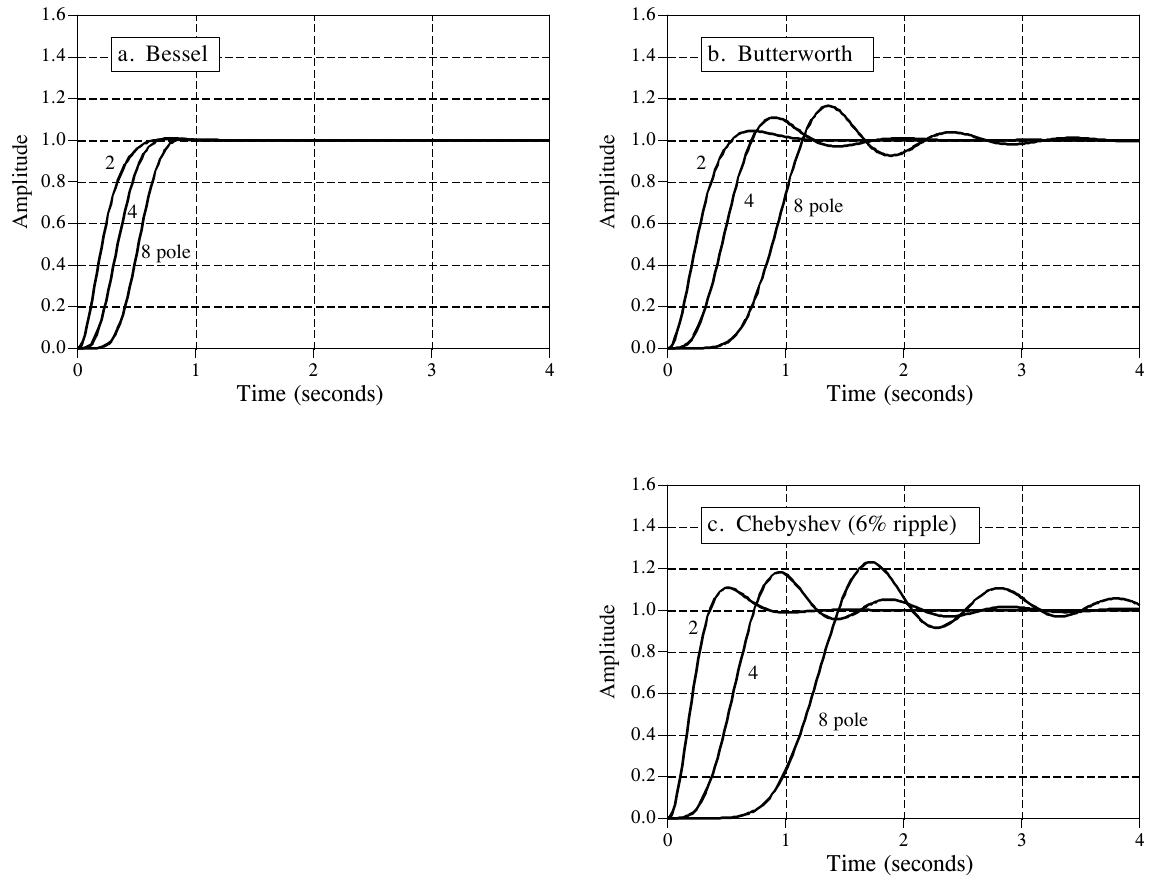
\includegraphics[width=0.971\linewidth,height=0.8\textheight,keepaspectratio]{assets/ch03/fig3-13.png}
\caption*{\textbf{图 3-13　三种滤波器的阶跃响应。} 横轴上的时间对应 1
赫兹的截止频率。在必须把过冲和振铃降到最低时，贝塞尔是最优的滤波器。
（a. 贝塞尔；b. 巴特沃斯；c.~切比雪夫（6\% 纹波）。曲线旁的 2 / 4 / 8
pole = 2/4/8 极点。Amplitude = 幅度，Time (seconds) = 时间（秒）。）}
\end{figure}

图 3-14 进一步说明了贝塞尔滤波器这个非常有利的特性。图 (a)
是一个脉冲波形，可以看作一个上升阶跃接着一个下降阶跃。图 (b) 和 (c)
分别是这个波形经过贝塞尔滤波器和切比雪夫滤波器后的样子。比如说，如果这是一个视频信号，切比雪夫滤波器引入的失真将是灾难性的！过冲会让物体边缘的亮度和中心不一样。更糟的是，物体的左侧会显得亮，右侧会显得暗。许多应用无法容忍阶跃响应表现差。这正是贝塞尔滤波器大显身手的地方：没有过冲，边缘对称。

\begin{figure}[htbp]
\centering
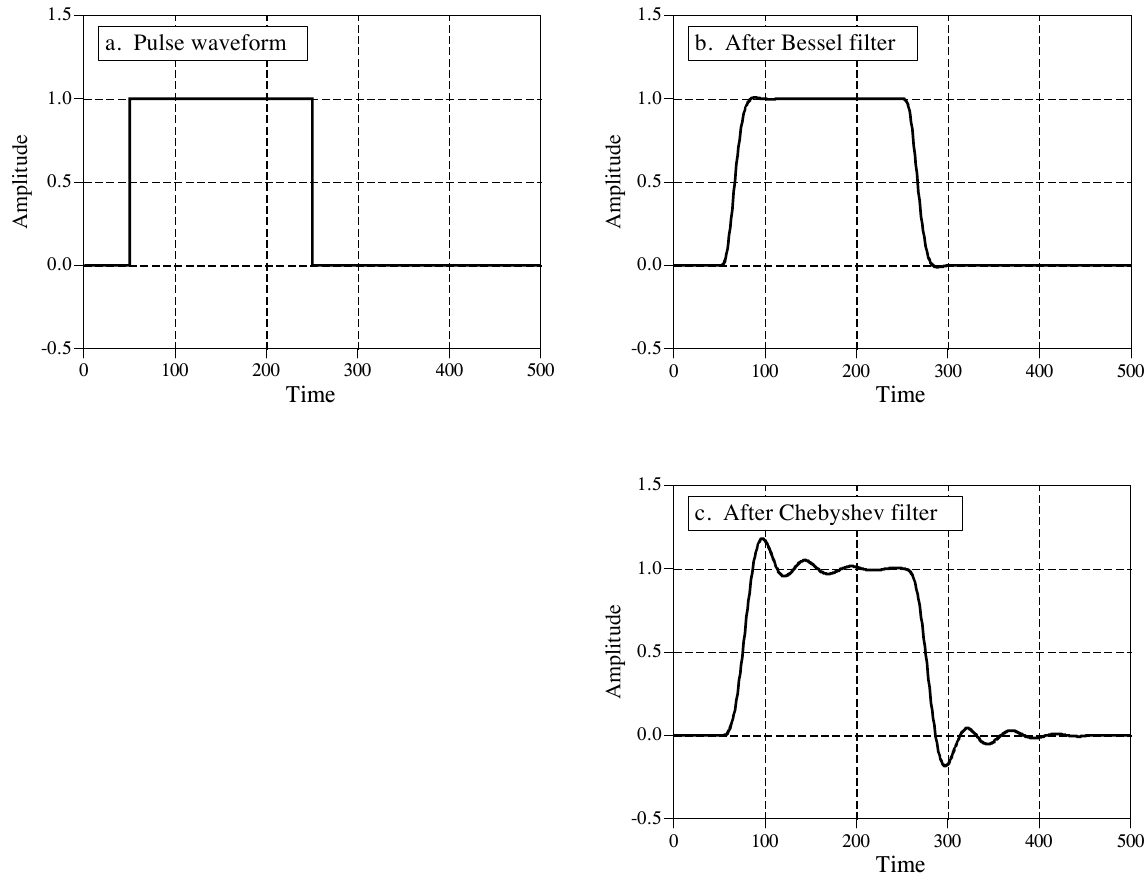
\includegraphics[width=0.954\linewidth,height=0.8\textheight,keepaspectratio]{assets/ch03/fig3-14.png}
\caption*{\textbf{图 3-14　贝塞尔滤波器和切比雪夫滤波器的脉冲响应。}
贝塞尔滤波器的一个关键特性是：滤波器输出中的上升沿和下降沿看起来相似。用这个领域的行话说，这叫线性相位(linear
phase)。图 (b) 是把 (a) 中的脉冲波形通过一个 4
极点贝塞尔滤波器的结果，两个边沿以相似的方式被平滑。图 (c) 是把 (a)
通过一个 4
极点切比雪夫滤波器的结果，左边沿在顶部过冲，右边沿在底部过冲。许多应用不能容忍这种失真。
（a. 脉冲波形(Pulse waveform)；b.
经过贝塞尔滤波器后；c.~经过切比雪夫滤波器后。Amplitude = 幅度，Time =
时间。）}
\end{figure}

\section{如何选择抗混叠滤波器}

表 3-2
总结了这三种滤波器的特性，说明每一种都是以牺牲其他一切为代价来优化某一个参数的：切比雪夫优化滚降，巴特沃斯优化通带平坦度，贝塞尔优化阶跃响应。

\textbf{表 3-2　三种经典滤波器的特性。}
贝塞尔滤波器的阶跃响应最好，因此是时域编码信号的首选。切比雪夫和巴特沃斯滤波器用于消除阻带中的频率，因此非常适合频域编码信号。表中数值的单位是秒和赫兹，对应
1 赫兹的截止频率。

\begingroup\scriptsize\setlength{\tabcolsep}{3pt}

{\def\LTcaptype{none} % do not increment counter
\begin{longtable}[]{@{}
  >{\raggedright\arraybackslash}p{(\linewidth - 16\tabcolsep) * \real{0.0882}}
  >{\raggedright\arraybackslash}p{(\linewidth - 16\tabcolsep) * \real{0.0882}}
  >{\raggedleft\arraybackslash}p{(\linewidth - 16\tabcolsep) * \real{0.1176}}
  >{\raggedleft\arraybackslash}p{(\linewidth - 16\tabcolsep) * \real{0.1176}}
  >{\raggedleft\arraybackslash}p{(\linewidth - 16\tabcolsep) * \real{0.1176}}
  >{\raggedleft\arraybackslash}p{(\linewidth - 16\tabcolsep) * \real{0.1176}}
  >{\raggedleft\arraybackslash}p{(\linewidth - 16\tabcolsep) * \real{0.1176}}
  >{\raggedleft\arraybackslash}p{(\linewidth - 16\tabcolsep) * \real{0.1176}}
  >{\raggedleft\arraybackslash}p{(\linewidth - 16\tabcolsep) * \real{0.1176}}@{}}
\toprule\noalign{}
\begin{minipage}[b]{\linewidth}\raggedright
滤波器
\end{minipage} & \begin{minipage}[b]{\linewidth}\raggedright
极点数
\end{minipage} & \begin{minipage}[b]{\linewidth}\raggedleft
直流电压增益
\end{minipage} & \begin{minipage}[b]{\linewidth}\raggedleft
过冲
\end{minipage} & \begin{minipage}[b]{\linewidth}\raggedleft
稳定到 1\% 的时间
\end{minipage} & \begin{minipage}[b]{\linewidth}\raggedleft
稳定到 0.1\% 的时间
\end{minipage} & \begin{minipage}[b]{\linewidth}\raggedleft
通带纹波
\end{minipage} & \begin{minipage}[b]{\linewidth}\raggedleft
衰减 100 倍的频率
\end{minipage} & \begin{minipage}[b]{\linewidth}\raggedleft
衰减 1000 倍的频率
\end{minipage} \\
\midrule\noalign{}
\endhead
\bottomrule\noalign{}
\endlastfoot
贝塞尔 & 2 & 1.27 & 0.4\% & 0.60 & 1.12 & 0\% & 12.74 & 40.4 \\
& 4 & 1.91 & 0.9\% & 0.66 & 1.20 & 0\% & 4.74 & 8.45 \\
& 6 & 2.87 & 0.7\% & 0.74 & 1.18 & 0\% & 3.65 & 5.43 \\
& 8 & 4.32 & 0.4\% & 0.80 & 1.16 & 0\% & 3.35 & 4.53 \\
巴特沃斯 & 2 & 1.59 & 4.3\% & 1.06 & 1.66 & 0\% & 10.0 & 31.6 \\
& 4 & 2.58 & 10.9\% & 1.68 & 2.74 & 0\% & 3.17 & 5.62 \\
& 6 & 4.21 & 14.3\% & 2.74 & 3.92 & 0\% & 2.16 & 3.17 \\
& 8 & 6.84 & 16.4\% & 3.50 & 5.12 & 0\% & 1.78 & 2.38 \\
切比雪夫 & 2 & 1.84 & 10.8\% & 1.10 & 1.62 & 6\% & 12.33 & 38.9 \\
& 4 & 4.21 & 18.2\% & 3.04 & 5.42 & 6\% & 2.59 & 4.47 \\
& 6 & 10.71 & 21.3\% & 5.86 & 10.4 & 6\% & 1.63 & 2.26 \\
& 8 & 28.58 & 23.0\% & 8.34 & 16.4 & 6\% & 1.34 & 1.66 \\
\end{longtable}
}

\endgroup

（原表把「直流电压增益」到「稳定到 0.1\% 的时间」归为阶跃响应(Step
Response)，后三列归为频率响应(Frequency Response)。）

抗混叠滤波器的选择，几乎完全取决于一个问题：你打算处理的信号是怎样表示信息的。在模拟波形中编码信息的方式有很多，但常见的只有两种：时域编码(time
domain encoding)和频域编码(frequency domain encoding)。这两者的区别在
DSP 中至关重要，也会是贯穿本书的一个反复出现的主题。

在频域编码中，信息包含在组合成信号的那些正弦波里。音频信号就是一个极好的例子。人听语音或音乐时，感知到的声音取决于其中存在哪些频率，而不是波形的具体形状。可以这样证明：让音频信号通过一个电路，这个电路改变各个正弦波的相位，但保留它们的频率和幅度。得到的信号在示波器上看起来完全不同，听起来却一模一样。尽管波形被大大改变了，有用的信息却完好无损。由于混叠会把频率成分放错位置并让它们重叠，它会直接破坏在频域中编码的信息。因此，这类信号的数字化通常要配一个截止陡峭的抗混叠滤波器，比如切比雪夫、椭圆或巴特沃斯滤波器。那这些滤波器糟糕的阶跃响应怎么办？无所谓，编码的信息不受这种失真的影响。

相反，时域编码用波形的形状来存储信息。例如，医生可以在病人的胸部和手臂上贴电极（心电图，electrocardiogram，简称
EKG），监测心脏的电活动。EKG
波形的形状提供了所需的信息，比如心跳过程中各个心腔在什么时候收缩。图像是这类信号的另一个例子。图像不是随时间变化的波形，而是把信息编码在随距离变化的波形形状中。图片由一块块亮度和颜色区域构成，以及它们和其他亮度、颜色区域之间的关系。你看《蒙娜丽莎》时不会说：「哇，好一组有趣的正弦波。」

问题就在这里：采样定理分析的是数字化过程中频域里发生了什么。这让它非常适合用来理解那些信息编码在频域中的信号的模数转换。然而，对于理解时域编码信号应该怎样数字化，采样定理帮不上什么忙。我们来仔细看看。

图 3-15 说明了数字化时域编码信号的几种选择。图 (a)
是一个待数字化的模拟信号示例。这里我们想捕获的信息是矩形脉冲的形状。这个示例信号中还包含一小段高频正弦波的猝发(burst)，它代表模拟信号上总会出现的宽带噪声、干扰之类的垃圾。其他几幅图显示了在不同抗混叠滤波器选项下数字化信号的样子：切比雪夫滤波器、贝塞尔滤波器，以及不用滤波器。

重要的是要明白，这些选项都无法让原始信号从采样数据中重建出来。这是因为原始信号本身就包含高于采样率一半的频率成分。既然这些频率不可能存在于数字化信号中，重建出来的信号也就不可能包含它们。这些高频有两个来源：(1)
噪声和干扰，这是你想消除的；(2)
波形中的陡峭边沿，其中很可能包含你想保留的信息。

\begin{enumerate}
\def\labelenumi{(\alph{enumi})}
\setcounter{enumi}{1}
\item
  中的切比雪夫滤波器解决问题的方式，是大刀阔斧地去掉所有高频成分。这样得到的滤波后模拟信号可以被采样，之后再完美重建。然而，重建出的模拟信号和滤波后的信号相同，而不是和原始信号相同。虽然采样过程中没有丢失任何东西，但波形已经被抗混叠滤波器严重扭曲了。如
  (b) 所示，这药方比病本身还糟！别这么干！
\item
  中的贝塞尔滤波器正是为这个问题设计的。它的输出和原始波形非常相似，只是边沿被温和地磨圆了。调整滤波器的截止频率，可以在边沿的平滑程度和消除信号中高频成分之间做取舍。滤波器用更多的极点，能在这两个参数之间取得更好的平衡。一条常用的经验法则是把截止频率设为采样频率的大约四分之一。这样每个边沿的上升段上大约有两个采样。注意贝塞尔和切比雪夫滤波器都去掉了原始信号中的那段高频噪声猝发。
\end{enumerate}

最后一种选择是完全不用抗混叠滤波器，如 (d)
所示。它有一个很大的优点：每个采样的值都和原始模拟信号的值相同。换句话说，它的边沿锐度是完美的：原始信号的变化会立即反映在数字数据中。缺点是混叠会扭曲信号。这有两种不同的表现形式。第一，高频干扰和噪声（比如示例中的正弦猝发）会变成毫无意义的采样，如
(d)
所示。也就是说，模拟信号中的任何高频噪声，都会以混叠噪声的形式出现在数字信号中。从更一般的意义上说，这不是采样的问题，而是上游模拟电路的问题。降低噪声和干扰不是
ADC
的职责，而是数字化之前的模拟电路的责任。结果可能是应该在数字化器之前放一个贝塞尔滤波器来控制这个问题。但这意味着这个滤波器应被视为模拟处理的一部分，而不是为了数字化器而做的事。

混叠的第二种表现更微妙。当模拟信号中发生某个事件（比如一个边沿）时，(d)
中的数字信号要到下一个采样才能察觉这个变化。数字数据中没有任何信息表明两个采样之间发生了什么。现在，就这个问题比较一下不用滤波器和用贝塞尔滤波器。例如，设想在
(c)
的采样之间画直线。这条构造出来的直线穿过阶跃幅度一半的那个时刻，就给出了模拟信号中边沿发生时刻的亚采样(subsample)估计。不用滤波器时，这种亚采样信息就完全丢失了。要评估这对你的具体情况有什么影响，用不着什么高深的定理，只需要清楚地知道数据采集到之后你打算拿它做什么。

\section{多速率数据转换}

电子学中有一股用数字算法取代模拟电路的强劲趋势，数据转换就是一个极好的例子。考虑设计一个数字录音机：这个系统要把语音信号数字化，以数字形式存储数据，之后再重建信号用于回放。要再现可懂的语音，系统必须捕获大约
100 到 3000
赫兹之间的频率。然而，麦克风产生的模拟信号还包含高得多的频率，比如高达
40 kHz。蛮力做法是让模拟信号通过一个截止频率为 3 kHz 的 8
极点低通切比雪夫滤波器，再以 8 kHz 采样。在另一端，DAC 用零阶保持以 8
kHz 重建模拟信号，再用另一个 3 kHz 的切比雪夫滤波器得到最终的语音信号。

\begin{figure}[htbp]
\centering
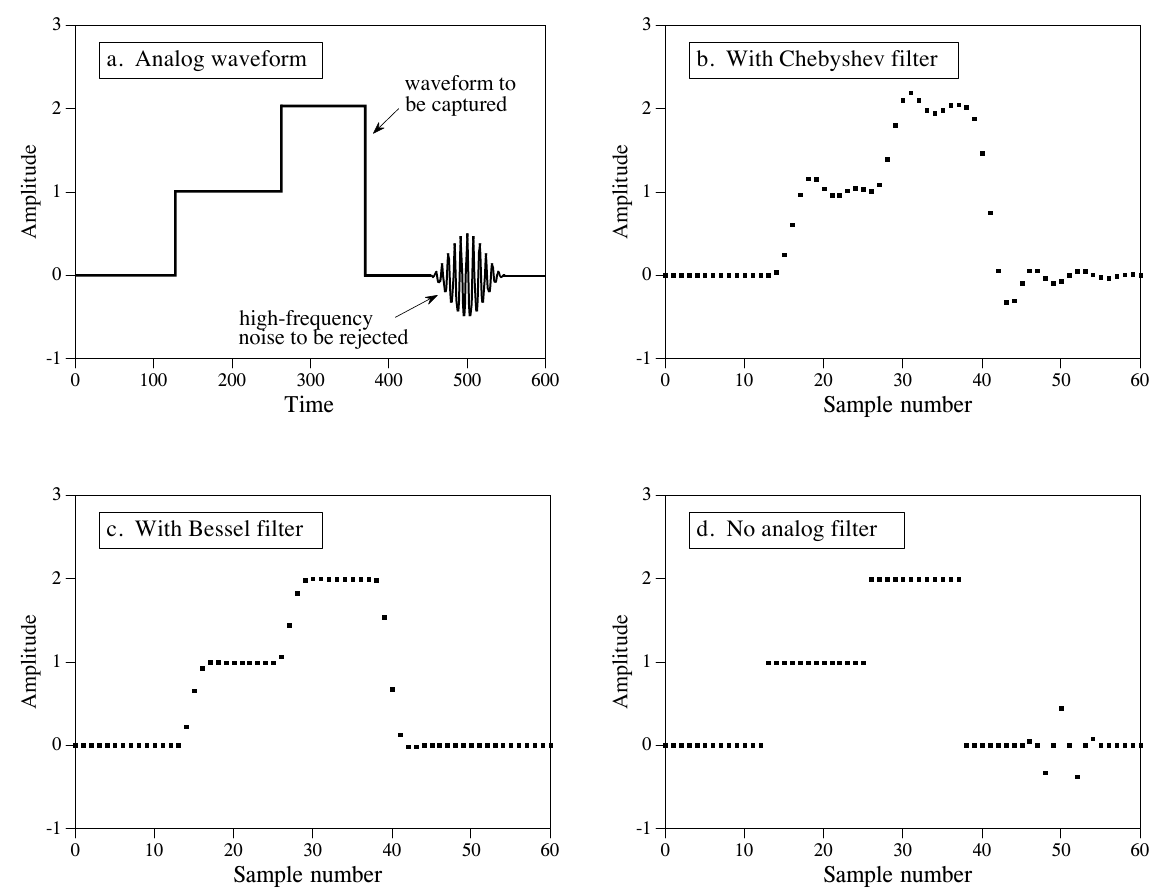
\includegraphics[width=0.967\linewidth,height=0.8\textheight,keepaspectratio]{assets/ch03/fig3-15.png}
\caption*{\textbf{图 3-15　时域编码信号的三种抗混叠滤波方案。}
目标是消除（采样时会混叠的）高频，同时保留（承载信息的）边沿锐度。图 (a)
是一个既有陡峭边沿、又有一段高频噪声猝发的模拟信号示例。图 (b)
是用切比雪夫滤波器得到的数字化信号。高频虽然被有效去除了，边沿却被严重扭曲。这通常是个糟糕的方案。(c)
中的贝塞尔滤波器在去除高频的同时，只对边沿做了温和的平滑。图 (d)
是不用抗混叠滤波器得到的数字化信号。这时边沿保持了完美的锐度，但高频猝发混叠成了几个毫无意义的采样。
（a. 模拟波形(Analog waveform)，waveform to be captured =
要捕获的波形，high-frequency noise to be rejected = 要滤除的高频噪声；b.
用切比雪夫滤波器；c.~用贝塞尔滤波器；d.~不用模拟滤波器。Amplitude =
幅度，Time = 时间，Sample number = 采样序号。）}
\end{figure}

以比这种直接分析更快的速率采样，有许多实用的好处。例如，设想用 64 kHz
的采样率重新设计这个数字录音机。抗混叠滤波器的任务变容易了：让 3 kHz
以下的所有频率通过，同时阻断 32 kHz
以上的所有频率。重建滤波器也有类似的简化。简而言之，更高的采样率让 8
极点滤波器可以换成简单的电阻-电容（RC）网络。问题在于，数字系统现在被更高采样率带来的数据淹没了。

更进一步的做法是多速率技术，即在同一个系统中使用不止一种采样率。以数字录音机为例，它是这样工作的。第一，让语音信号通过一个简单的
RC 低通滤波器，以 64 kHz 采样。得到的数字数据包含所需的 100 到 3000
赫兹语音频带，也包含 3 kHz 到 32 kHz
之间不可用的频带。第二，在软件中用一个 3 kHz
的数字低通滤波器去掉这些不可用的频率。第三，把数字信号从 64 kHz 重采样到
8 kHz，做法就是每 8 个采样丢掉 7
个，这个过程叫抽取(decimation)。得到的数字数据，等同于用激进的模拟滤波加上直接
8 kHz 采样所得到的数据。

多速率技术也可以用在这个示例系统的输出部分。从存储器中取出 8 kHz
的数据，把它转换成 64 kHz
的采样率，这个过程叫插值(interpolation)。做法是在从存储器取出的每两个采样之间插入七个值为零的采样。得到的信号是一个数字冲激串，包含所需的
100 到 3000 赫兹语音频带，以及 3 kHz 到 32 kHz 之间的频谱复制。回头看图
3-6 的 (a) 和 (b) 就能明白为什么会这样。然后用一个数字低通滤波器去掉 3
kHz 以上的一切。经 DAC 转换成模拟信号后，只需要一个简单的 RC
网络就能得到最终的语音信号。

多速率数据转换的价值有两点：(1)
它用软件取代了模拟元件，这在大批量生产的产品中有明显的经济优势；(2)
它能在关键应用中达到更高的性能水平。例如，CD
音频系统就用这类技术获得尽可能好的音质。性能的提升来自用数字算法（舍入误差带来的精度为
0.0001\%）取代模拟元件（精度
1\%）。后面的章节会讲到，数字滤波器在一些关键方面比模拟滤波器强几百倍。

\section{单比特数据转换}

单比特 ADC 和 DAC
是电信和高保真音乐重放中一种流行的技术。它们属于多速率技术，用更高的采样率换取更少的比特数。极端情况下，每个采样只需要一个比特。电路结构虽然多种多样，但大多基于增量调制(delta
modulation)。下面介绍三个示例电路，让你对这个领域有个大致的感觉。这些电路都做在集成电路里，所以不用操心每个晶体管和运放该放在哪里。没人会要你用基本元件搭一个这样的电路。

图 3-16
是一个典型增量调制器的框图。模拟输入是一个幅度为几伏的语音信号，输出信号是一串数字
1 和
0。比较器(comparator)判断进入的模拟信号和电容上存储的电压哪个更高。这个判断以数字
1 或 0
的形式送到锁存器(latch)的输入端。在每个时钟脉冲（通常是几百千赫兹）到来时，锁存器把输入端出现的数字状态传到输出端。这个锁存器保证输出与时钟同步，从而确定了采样率，即
1 比特输出能够更新自己的速率。

\begin{figure}[htbp]
\centering
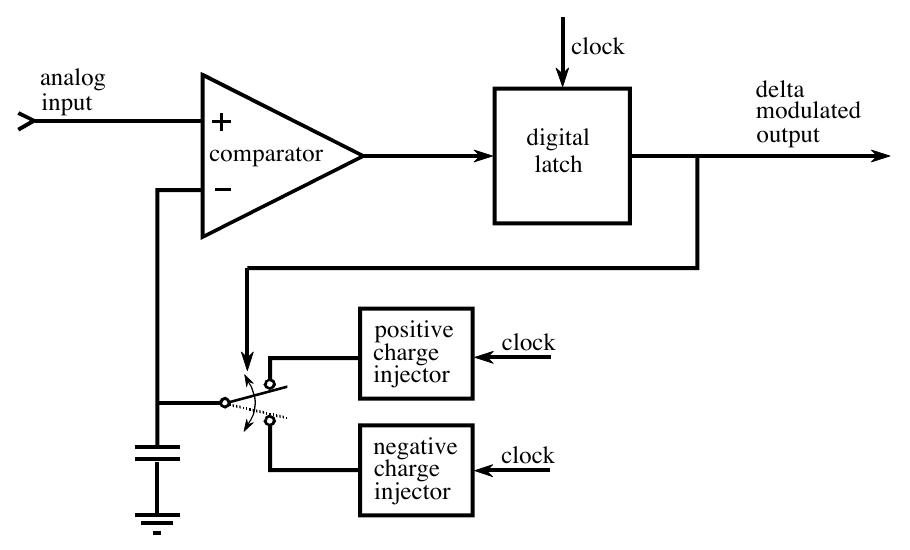
\includegraphics[width=0.758\linewidth,height=0.8\textheight,keepaspectratio]{assets/ch03/fig3-16.png}
\caption*{\textbf{图 3-16　增量调制电路框图。}
输入电压与电容上存储的电压比较，结果以数字 0 或 1
送到锁存器的输入端。锁存器的输出与时钟同步更新，并用在一个反馈回路中，使电容电压跟踪输入电压。
（analog input = 模拟输入，comparator = 比较器，latch = 锁存器，clock =
时钟，delta modulated digital output = 增量调制的数字输出，positive /
negative charge injector = 正/负电荷注入器。）}
\end{figure}

把数字输出拿来驱动一个电子开关，就形成了反馈回路。如果输出是数字
1，开关把电容接到正电荷注入器(positive charge
injector)。这是一个很宽泛的说法，指的是每个时钟周期把电容上的电压提高一个固定量（比如
1 毫伏）的电路。它可能只是一个接到较高正电压的电阻。如果输出是数字
0，开关接到负电荷注入器，它把电容上的电压降低同样的固定量。

图 3-17
说明了这个电路产生的信号。在时间为零时，模拟输入和电容上的电压都从零开始。如
(a) 所示，输入信号在第八个时钟周期突然升到 9.5
伏。由于输入信号现在比电容上的电压更正，数字输出变为 1，如 (b)
所示。这使开关接到正电荷注入器，电容上的电压在每个时钟周期增加一小步。虽然
(a) 中画的是每个时钟周期增加 1 伏，但这只是为了示意，更典型的值是 1
毫伏。电容电压的这种阶梯式上升一直持续到它超过输入信号的电压为止。此时系统达到平衡，输出在数字
1 和 0 之间振荡，使电容上的电压在 9 伏和 10
伏之间振荡。就这样，电路的反馈迫使电容电压跟踪输入信号的电压。如果输入信号变化得非常快，电容上的电压会以恒定的速率变化，直到追上为止。这个恒定的变化率叫压摆率(slew
rate)，和运放等其他电子器件中的叫法一样。

现在来看增量调制输出信号的特性。如果模拟输入的值在增加，输出信号中 1
会比 0 多。同样，如果模拟输入的值在减小，输出中 0 会比 1
多。如果模拟输入恒定，数字输出会在 0 和 1
之间交替，两者个数相等。说得更一般些，1 和 0
的相对数量与模拟输入的斜率（导数(derivative)）成正比。

\begin{figure}[htbp]
\centering
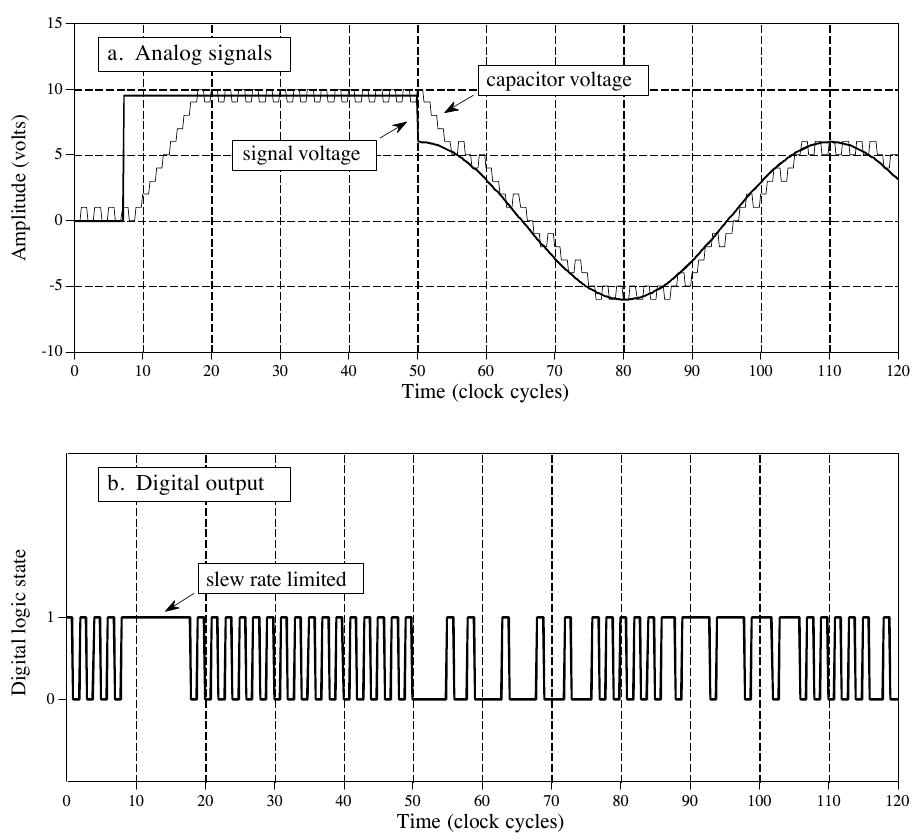
\includegraphics[width=0.767\linewidth,height=0.8\textheight,keepaspectratio]{assets/ch03/fig3-17.png}
\caption*{\textbf{图 3-17　图 3-16 中增量调制器产生的信号示例。} 图 (a)
是模拟输入信号以及电容上对应的电压。图 (b) 是增量调制的输出，即一串数字
1 和 0。 （a. 模拟信号(Analog signals)：capacitor voltage =
电容电压，signal voltage = 信号电压，Amplitude (volts) = 幅度（伏）；b.
数字输出(Digital output)：Digital logic state = 数字逻辑状态，slew rate
limited = 受压摆率限制。Time (clock cycles) = 时间（时钟周期）。）}
\end{figure}

这个电路是把模拟信号转换成一串串行的 1 和
0、用于传输或数字存储的廉价方法。一个特别吸引人的特点是：所有比特的含义都相同，不像传统的串行格式那样分为起始位、LSB、\ldots、MSB、停止位。接收端的电路和发送电路的反馈部分完全相同。正如发送电路中电容上的电压跟随模拟输入一样，接收电路中电容上的电压也是如此。也就是说，(a)
中的电容电压也代表了重建信号的样子。

这个电路的一个关键局限，是 (1) 最大压摆率、(2) 量化步长和 (3)
数据率三者之间不可避免的权衡。具体来说，如果把最大压摆率和量化步长调到语音通信可以接受的值，数据率最终会落在
MHz 量级。这太高了，没有商业价值。例如，常规的语音信号采样只需要每秒约
64,000 比特。

图 3-18 给出了这个问题的一个解决方案：连续可变斜率增量(CVSD,
Continuously Variable Slope Delta)调制器，摩托罗拉 MC3518
系列实现了这一技术。这种方法把时钟速率和量化步长设成可以接受的值，比如
30 kHz 和 2000
级。这会导致压摆率非常差，于是用附加电路来校正。工作时，一个移位寄存器(shift
register)持续观察系统最近产生的四个比特。如果电路处于受压摆率限制的状态，最近四个比特就会全是
1（正斜率）或全是
0（负斜率）。一个逻辑电路检测到这种情况，产生一个模拟信号，提高电荷注入器产生的电荷量。这通过增大加到电容上的电压步长来提高压摆率。

逻辑电路和电荷注入器之间通常会放一个模拟滤波器。这让步长取决于电路已经处于压摆受限状态多长时间。只要电路一直压摆受限，步长就会越来越大。这常被称为音节滤波器(syllabic
filter)，因为它的特性取决于构成语音的音节的平均长度。经过适当的优化（来自芯片厂商的规格书，而不是你自己的工作），16
到 32 kHz
的数据率就能产生质量可接受的语音。不断变化的步长让数字数据很难看懂，但幸运的是，你也不需要看懂。在接收端，用一个和发送电路中完全相同的音节滤波器来重建模拟信号。如果两个滤波器匹配，CVSD
调制带来的失真就很小。CVSD 可能是以数字方式传输语音信号最简单的方法。

\begin{figure}[htbp]
\centering
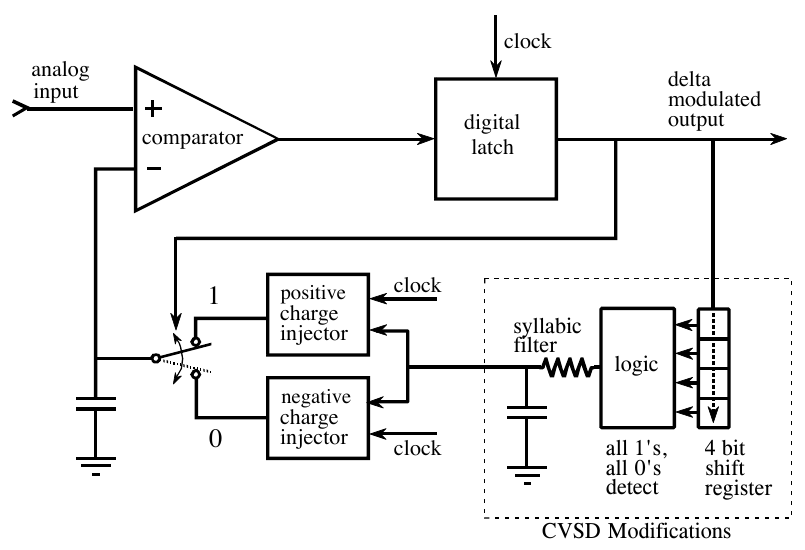
\includegraphics[width=0.671\linewidth,height=0.8\textheight,keepaspectratio]{assets/ch03/fig3-18.png}
\caption*{\textbf{图 3-18　CVSD 调制框图。}
在基本的增量调制器上加了一个逻辑电路，以改善压摆率。 （在图 3-16
的基础上新增「CVSD Modifications = CVSD 改动」部分：4 bit shift register
= 4 比特移位寄存器，all 1's, all 0's detect = 全 1/全 0 检测，logic =
逻辑电路，syllabic filter = 音节滤波器。）}
\end{figure}

CVSD
调制虽然非常适合编码语音信号，却不能用于通用的模数转换。即使你能绕开「数字数据与输入信号的导数相关」这一点，变化的步长也会把事情搞得无法收拾。此外，模拟信号的直流电平通常不会被数字数据捕获。

图 3-19 所示的增量-累加转换器(delta-sigma converter)，巧妙地把模拟电路和
DSP
算法结合起来，消除了这些问题。注意电容上的电压现在是和地电位比较。反馈回路也做了修改：电路输出数字
1 时，电容上的电压降低；输出数字 0
时，电压升高。当输入信号的电压升高和降低时，它会试图抬高和压低电容上的电压。比较器检测到这种电压变化，于是电荷注入器产生抵消的电荷，使电容保持在零伏。

如果输入电压为正，数字输出中 1 会比 0 多，多出来的 1
用来产生负电荷，与正的输入信号抵消。同样，如果输入电压为负，数字输出中 0
会比 1 多，提供净的正电荷注入。如果输入信号等于零伏，输出中 1 和 0
的个数相等，总的电荷注入为零。

现在，输出中 1 和 0
的相对数量与输入电压的电平相关，而不是像前一个电路那样与斜率相关。这就简单多了。例如，把数字输出送进一个计数器，统计
4096 个时钟周期里 1 的个数，就构成了一个 12 比特 ADC。数字 4095
对应最大的正输入电压，数字 0 对应最大的负输入电压，2048
对应零输入电压。这也说明了「增量-累加(delta-sigma)」这个名字的由来：先做增量调制(delta)，再做求和(sigma)。

\begin{figure}[htbp]
\centering
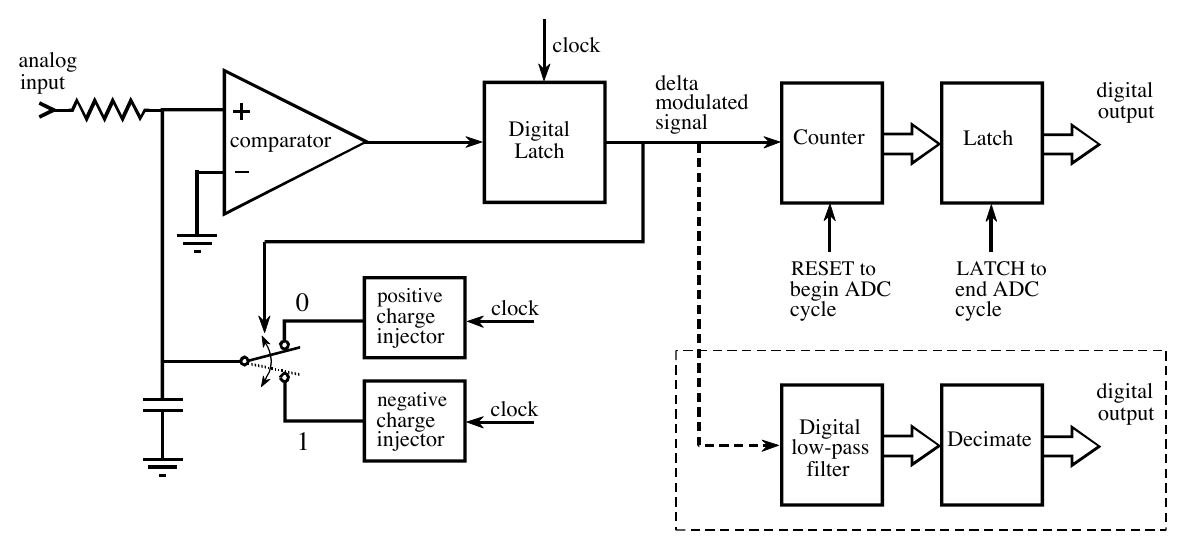
\includegraphics[width=0.983\linewidth,height=0.8\textheight,keepaspectratio]{assets/ch03/fig3-19.png}
\caption*{\textbf{图 3-19　增量-累加模数转换器框图。}
最简单的情况下，对增量调制器输出的脉冲计数，计满预定的时钟周期数，然后锁存计数器的输出，完成一次转换。在更复杂的电路中，脉冲先经过一个数字低通滤波器，再重采样（抽取）到较低的采样率。
（delta modulated signal = 增量调制信号，Digital Counter =
数字计数器，Latch = 锁存器，RESET to begin ADC cycle = 复位以开始一次
ADC 周期，LATCH to end ADC cycle = 锁存以结束一次 ADC 周期，Digital
low-pass filter = 数字低通滤波器，Decimate = 抽取，digital output =
数字输出。）}
\end{figure}

这类增量调制器产生的 1 和
0，很容易变回模拟信号。只需要一个模拟低通滤波器，可能简单到只是一个 RC
网络。数字 1 和 0
对应的高低电压平均下来，就形成正确的模拟电压。例如，假设 1 和 0 分别用 5
伏和 0 伏表示。如果数据流中 80\% 的比特是 1、20\% 是
0，低通滤波器的输出就是 4 伏。

这种把单比特数据流变回原始波形的方法，因为几个原因而很重要。第一，它提供了一种取代增量-累加
ADC
电路中计数器的巧妙办法：不再简单地对增量调制器输出的脉冲计数，而是让这个二值信号通过一个数字低通滤波器，再抽取以降低采样率。例如，这个过程可能先把数字流中的每个
1 和 0 变成一个 12 比特的采样：1 变成 4095，0 变成
0。对这个信号做数字低通滤波，就得到原始波形的数字化版本，正如模拟低通滤波器会得到模拟复现一样。然后抽取丢掉大部分采样，降低采样率。结果得到的数字信号，等同于对原始波形直接采样。

许多商用 ADC
用这种方法数字化语音和其他音频信号。一个例子是美国国家半导体(National
Semiconductor)的 ADC16071，它能以最高 192 kHz 的采样率做 16
比特模数转换。采样率为 100 kHz 时，增量调制器的时钟频率为 6.4
MHz。数字低通滤波器是一个 246 点的 FIR 滤波器，第 16
章会介绍这种滤波器。它去掉数字数据中 50
kHz（最终采样率的一半）以上的所有频率。从概念上说，可以把它看作形成了一个
6.4 MHz、每个采样 16 比特的数字信号。然后把信号从 6.4 MHz 抽取到 100
kHz，做法是每 64 个采样删掉 63
个。实际工作中，这个器件内部发生的事情比这段简单讨论描述的要多得多。

增量-累加转换器也可以用于语音和音频信号的数模转换。从存储器中取出数字信号，把它转换成增量调制的
1 和 0
流。如上所述，用一个简单的模拟低通滤波器，就能很容易地把这个单比特信号变成重建的模拟信号。和抗混叠滤波器一样，通常只需要一个
RC 网络。这是因为大部分滤波工作都由高性能的数字滤波器完成了。

增量-累加 ADC
有几个怪癖，限制了它们只能用于特定的应用。例如，很难对它们的输入做多路复用(multiplex)。当输入从一个信号切换到另一个信号时，要等数字滤波器把前一个信号的数据清空之后，才能恢复正常工作。增量-累加转换器在另一方面也有局限：你不知道每个采样确切是在什么时刻取的。每个采到的采样，都是在输入信号的一段区间上取得的
1
比特信息的综合。对于音频这类频域编码的信号，这不是问题；但对于时域编码的信号，这是一个重大的局限。要理解信号波形的形状，你常常需要知道每个采样被取的精确时刻。最后，这些器件大多是专门为音频应用设计的，它们的性能指标也是相应地给出的。例如，一个用于语音信号的
16 比特 ADC，并不一定意味着每个采样都有 16
比特的精密度。更可能的是，厂商的意思是语音信号可以被数字化到 16
比特的动态范围(dynamic
range)。别指望在通用数据采集中从这种器件得到完整的 16 比特有用信息。

这些解释和例子虽然介绍了单比特 ADC 和 DAC，但必须强调，它们只是对复杂的
DSP
和集成电路技术的简化描述。你不会指望厂商把芯片的全部内部工作原理告诉竞争对手，所以也别指望他们会告诉你。

% !TEX root = ../main.tex
% 本文件由 build-tex.sh 从 04-DSP指南-第4章中译.md 生成，改内容请改 md 后重新生成

\chapter{DSP 软件}\label{ch-04}

DSP 应用程序通常和其他科学、工程任务一样，用 C、BASIC
和汇编等语言编写。C
的强大和通用性，使它成为计算机科学家和其他专业程序员的首选语言。另一方面，BASIC
的简单，使它非常适合那些只是偶尔涉足编程世界的科学家和工程师。无论你用什么语言，大多数重要的
DSP 软件问题都深埋在底层那个 0 和 1
飞旋的世界里。这包括这样一些话题：数字怎样用比特模式(bit
pattern)表示、计算机运算中的舍入误差、不同类型处理器的计算速度等。本章讲的是你能在高层做些什么，以免被计算机底层的内部运作踩在脚下。

\section{计算机里的数}

数字计算机非常擅长存储和调取数字，可惜这个过程并非没有误差。例如，你让计算机存储数字
1.41421356。计算机尽力而为，存下它能表示的最接近的数：1.41421354。有时这个误差无关紧要，有时却是灾难性的。再举一个例子，一个经典的计算错误来自两个大小相差悬殊的数相加，比如
1 和 0.00000001。我们希望答案是 1.00000001，计算机却回答
1。理解计算机怎样存储和处理数字，能让你在程序吐出毫无意义的数据之前，就预见并纠正这些问题。

这些问题的根源在于：每个数都只分配了固定数目的比特来存储，通常是
8、16、32 或 64 位。例如，考虑用 8 个比特存储一个变量的值。由于只有
\(2^8 = 256\) 种可能的比特模式，这个变量只能取 256
个不同的值。这是这种情况的根本局限，我们对此无能为力。我们能控制的是：规定每个比特模式代表什么值。最简单的情况下，这
256 个比特模式可以代表 0 到 255、1 到 256、−127 到 128
等整数。在一种更不寻常的方案里，这 256 个比特模式可以代表 256
个按指数关系排列的数：1、10、100、1000、\ldots、\(10^{254}\)、\(10^{255}\)。每个访问这些数据的人都必须明白每个比特模式代表什么值。这通常由一个算法或公式给出，用来在所代表的值和对应的比特模式之间来回转换。

可能的编码方案虽然很多，但常用的只有两种通用格式：定点数(fixed
point，也叫整数)和浮点数(floating point，也叫实数)。在本书的 BASIC
程序中，定点变量用名字最后一个字符为 \% 来标示，比如 I\%、N\%、SUM\%
等。其他变量都是浮点数，比如 X、Y、MEAN
等。在评估接下来几页介绍的格式时，试着从两方面去理解它们：范围(range，能表示的最大数和最小数)和精度(precision，相邻两个数之间的间隙大小)。

\section{定点数（整数）}

定点表示用来存储整数，即正负整数：\ldots、−3、−2、−1、0、1、2、3、\ldots。C
和 BASIC 这样的高级语言，通常给每个整数分配 16
个比特。最简单的情况下，\(2^{16} = 65,536\) 种可能的比特模式被分配给 0
到 65,535 这些数。这叫无符号整数(unsigned integer)格式，图 4-1
给出了一个简化的例子（每个数只用 4
个比特）。比特模式与所代表的数之间的转换，无非就是二进制(binary)和十进制(decimal)之间的换算。无符号整数的缺点是不能表示负数。

偏移二进制(offset
binary)和无符号整数类似，只是把十进制值整体平移，以便能表示负数。在图
4-1 的 4 比特例子中，十进制数偏移了 7，于是 16 个比特模式对应 −7 到 8
的整数。同样，16 比特表示会用 32,767 作偏移量，得到 −32,767 到 32,768
的范围。偏移二进制不是一种标准化的格式，你也会看到别的偏移量，比如
32,768。偏移二进制最重要的用途是在 ADC 和 DAC 中。例如，对于 12
比特转换，−5 V 到 5 V 的输入电压范围可能被映射到数字 0 到 4095。

原码(sign and
magnitude，符号-幅值表示)是另一种表示负整数的简单方法。最左边的比特叫符号位(sign
bit)，正数为 0，负数为
1。其余比特是这个数绝对值的标准二进制表示。这会浪费一个比特模式，因为零有两种表示：0000（正零）和
1000（负零）。这种编码方案使 16 比特数的范围是 −32,767 到 32,767。

\textbf{图 4-1　定点（整数）表示的常用格式。}
无符号整数是一种简单的二进制格式，但不能表示负数。偏移二进制和原码可以表示负数，但很难用硬件实现。补码最容易设计硬件，是通用计算中最常用的格式。

{\def\LTcaptype{none} % do not increment counter
\begin{longtable}[]{@{}
  >{\centering\arraybackslash}p{(\linewidth - 8\tabcolsep) * \real{0.2381}}
  >{\raggedleft\arraybackslash}p{(\linewidth - 8\tabcolsep) * \real{0.1905}}
  >{\raggedleft\arraybackslash}p{(\linewidth - 8\tabcolsep) * \real{0.1905}}
  >{\raggedleft\arraybackslash}p{(\linewidth - 8\tabcolsep) * \real{0.1905}}
  >{\raggedleft\arraybackslash}p{(\linewidth - 8\tabcolsep) * \real{0.1905}}@{}}
\toprule\noalign{}
\begin{minipage}[b]{\linewidth}\centering
比特模式
\end{minipage} & \begin{minipage}[b]{\linewidth}\raggedleft
无符号整数
\end{minipage} & \begin{minipage}[b]{\linewidth}\raggedleft
偏移二进制
\end{minipage} & \begin{minipage}[b]{\linewidth}\raggedleft
原码
\end{minipage} & \begin{minipage}[b]{\linewidth}\raggedleft
补码
\end{minipage} \\
\midrule\noalign{}
\endhead
\bottomrule\noalign{}
\endlastfoot
1111 & 15 & 8 & −7 & −1 \\
1110 & 14 & 7 & −6 & −2 \\
1101 & 13 & 6 & −5 & −3 \\
1100 & 12 & 5 & −4 & −4 \\
1011 & 11 & 4 & −3 & −5 \\
1010 & 10 & 3 & −2 & −6 \\
1001 & 9 & 2 & −1 & −7 \\
1000 & 8 & 1 & 0（负零） & −8 \\
0111 & 7 & 0 & 7 & 7 \\
0110 & 6 & −1 & 6 & 6 \\
0101 & 5 & −2 & 5 & 5 \\
0100 & 4 & −3 & 4 & 4 \\
0011 & 3 & −4 & 3 & 3 \\
0010 & 2 & −5 & 2 & 2 \\
0001 & 1 & −6 & 1 & 1 \\
0000 & 0 & −7 & 0 & 0 \\
\textbf{16 比特范围} & 0 到 65,535 & −32,767 到 32,768 & −32,767 到
32,767 & −32,768 到 32,767 \\
\end{longtable}
}

（原图按「十进制值 \dspsym{→}
比特模式」分四栏排列，这里改成以比特模式为行，便于横向比较同一个比特模式在四种格式下代表的值。）

前三种表示在概念上很简单，但很难用硬件实现。记住，当你在计算机程序中写下
A=B+C 时，某位硬件工程师得想出办法，让代表 B 的比特模式和代表 C
的比特模式结合，形成代表 A 的比特模式。

补码(two's
complement)是硬件工程师钟爱的格式，也是计算机中通常表示整数的方式。要理解它的编码模式，先看图
4-1 中十进制数 0，它对应二进制的零
0000。往上数时，十进制数就是对应的二进制数（0 = 0000，1 = 0001，2 =
0010，3 = 0011，等等）。现在记住，这四个比特存放在由 4
个触发器(flip-flop)组成的寄存器里。如果我们再从 0000
开始往下减，数字硬件会自动按补码计数：0 = 0000，−1 = 1111，−2 = 1110，−3
= 1101，等等。这就像新车的里程表：往前开，它变成
00000、00001、00002、00003\ldots\ldots；倒着开，里程表变成
00000、99999、99998、99997\ldots\ldots{}

用 16 个比特，补码能表示 −32,768 到 32,767
的数。如果数是正数或零，最左边的比特为 0；如果是负数，则为
1。因此，最左边的比特也叫符号位，和原码中一样。对于正数，十进制与补码之间的转换很直接，就是简单的十进制转二进制。对于负数，常用下面的算法：(1)
取十进制数的绝对值；(2) 把它转换成二进制；(3) 把所有比特取反（1 变 0，0
变 1）；(4) 二进制数加 1。例如：−5 \dspsym{→} 5 \dspsym{→} 0101
\dspsym{→} 1010 \dspsym{→}
1011。补码对人来说很难，对数字电路来说却很容易。

\section{浮点数（实数）}

浮点数的编码方案比定点数复杂。基本思想和科学记数法(scientific
notation)一样：一个尾数(mantissa)乘以 10 的某个指数(exponent)次幂。例如
\(5.4321 \times 10^6\)，其中 5.4321 是尾数，6
是指数。科学记数法特别擅长表示极大和极小的数。例如：\(1.2 \times 10^{50}\)，地球上的原子数；或者
\(2.6 \times 10^{-23}\)，乌龟一秒钟爬过的距离与我们银河系直径之比。注意，用科学记数法表示的数要做规格化(normalize)，使小数点左边只有一位非零数字。这是通过按需调整指数来实现的。

浮点表示和科学记数法类似，只是一切都以 2 为底而不是以 10
为底。类似的格式有好几种在用，最常见的是 ANSI/IEEE Std.
754-1985。这个标准定义了 32 比特数的格式，叫单精度(single
precision)；以及 64 比特数的格式，叫双精度(double precision)。如图 4-2
所示，单精度的 32 个比特分成三组：第 0 到 22 位构成尾数，第 23 到 30
位构成指数，第 31 位是符号位。这些比特按下面的关系构成浮点数 v：

\textbf{公式 4-1　把比特模式转换成浮点数的公式。} v 是所表示的数，S
是符号位的值，M 是尾数的值，E 是指数的值。

\[
v = (-1)^S \times M \times 2^{E-127}
\]

\((-1)^S\) 这一项的意思就是：符号位 S 为 0 时是正数，为 1 时是负数。变量
E 是八个指数比特所代表的 0 到 255 之间的数。把这个数减去
127，指数项就能从 \(2^{-127}\) 变到
\(2^{128}\)。换句话说，指数是以偏移量 127 的偏移二进制存储的。

尾数 M 由 23 个比特构成一个二进制小数。例如，十进制小数 2.783 解释为
\(2 + 7/10 + 8/100 + 3/1000\)。二进制小数 1.0101 的意思是
\(1 + 0/2 + 1/4 + 0/8 + 1/16\)。浮点数和科学记数法一样要规格化，即小数点（在二进制中叫二进制点(binary
point)）左边只有一位非零数字。由于二进制中唯一的非零数字是
1，尾数的首位总是
1，因此不必存储。去掉这个冗余，就让数多了一个比特的精度。存储的 23
个比特记作 \(m_{22}, m_{21}, m_{20}, \ldots, m_0\)，按下式构成尾数：

\textbf{公式 4-2　把比特模式转换成公式 4-1 所用的尾数 M 的算法。}

\[
M = 1.m_{22}m_{21}m_{20}m_{19}\cdots m_2m_1m_0
\]

换句话说，\(M = 1 + m_{22}2^{-1} + m_{21}2^{-2} + m_{20}2^{-3} + \cdots\)。如果第
0 到 22 位全为零，M 的值就是 1。如果第 0 到 22 位全为 1，M 就比 2
小一丁点，即 \(2 - 2^{-23}\)。

\begin{figure}[htbp]
\centering
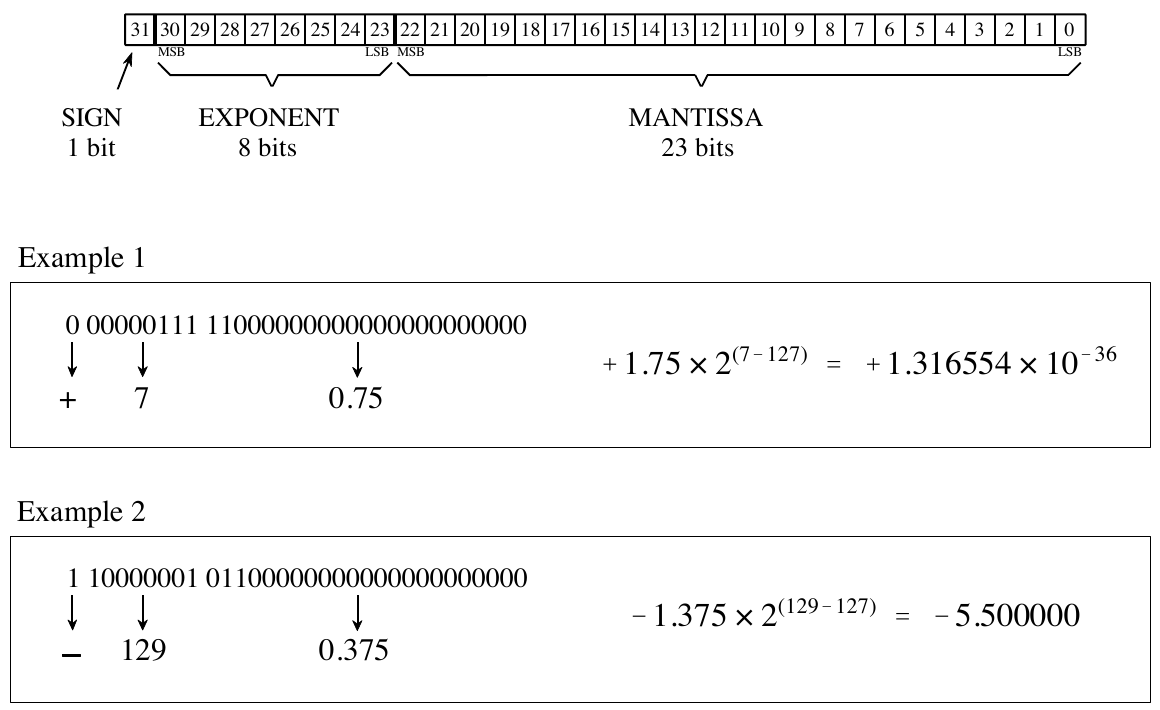
\includegraphics[width=0.967\linewidth,height=0.8\textheight,keepaspectratio]{assets/ch04/fig4-02.png}
\caption*{\textbf{图 4-2　单精度浮点数的存储格式。} 32
个比特分成三部分：符号位、指数和尾数。公式 4-1 和 4-2
说明了怎样由这三部分求出所表示的数。MSB 和 LSB
分别指「最高有效位」和「最低有效位」。 （SIGN = 符号，1 比特；EXPONENT =
指数，8 比特；MANTISSA = 尾数，23 比特。例 1：符号 +，指数 7，尾数
0.75，表示 \(+1.75 \times 2^{(7-127)} = +1.316554 \times 10^{-36}\)。例
2：符号 −，指数 129，尾数 0.375，表示
\(-1.375 \times 2^{(129-127)} = -5.500000\)。）}
\end{figure}

用这种编码方案，能表示的最大数是
\(\pm(2-2^{-23}) \times 2^{128} = \pm 6.8 \times 10^{38}\)。同样，能表示的最小数是
\(\pm 1.0 \times 2^{-127} = \pm 5.9 \times 10^{-39}\)。IEEE
标准把这个范围稍微缩小了一点，腾出一些比特模式赋予特殊含义。具体来说，标准允许的最大数和最小数分别是
\(\pm 3.4 \times 10^{38}\) 和
\(\pm 1.2 \times 10^{-38}\)。腾出来的比特模式用于三类特殊的数：(1)
±0，定义为尾数和指数的所有比特都为零。(2)
±\dspsym{∞}，定义为尾数的所有比特为零、指数的所有比特为 1。(3) 一组介于
\(\pm 1.2 \times 10^{-38}\) 和 \(\pm 1.4 \times 10^{-45}\)
之间的非常小的非规格化数(unnormalized
numbers)。这些数去掉了「尾数首位必须为
1」的要求，精度较低。除了这三类特殊数之外，还有一些没有被赋予含义的比特模式，通常称为
NAN（Not A Number，非数）。

IEEE 双精度标准只是给尾数和指数都加了更多比特。存储双精度数的 64
个比特中，第 0 到 51 位是尾数，第 52 到 62 位是指数，第 63
位是符号位。和前面一样，尾数在 1 和略小于 2 之间，即
\(M = 1 + m_{51}2^{-1} + m_{50}2^{-2} + m_{49}2^{-3} + \cdots\)。11
个指数比特构成 0 到 2047 之间的数，偏移量为 1023，允许指数从
\(2^{-1023}\) 到 \(2^{1024}\)。允许的最大数和最小数分别是
\(\pm 1.8 \times 10^{308}\) 和
\(\pm 2.2 \times 10^{-308}\)。这些数大得和小得不可思议！单精度不够用的应用相当少见。你大概永远不会遇到双精度限制你实现目标的情况。

\section{数值精度}

数值表示带来的误差，和 ADC
中的量化误差非常相似。你想存储一个连续范围的值，却只能表示有限个量化电平。每生成一个新数（比如做完一次数学计算之后），它都必须被舍入到你所用格式能存储的最接近的值。

举个例子，设想你分配 32 个比特来存储一个数。由于恰好有
\(2^{32} = 4,294,967,296\) 种不同的比特模式，你恰好能表示 4,294,967,296
个不同的数。有些编程语言提供一种叫长整型(long integer)的变量，以 32
比特、定点、补码形式存储。这意味着 4,294,967,296 种可能的比特模式代表
−2,147,483,648 到 2,147,483,647 之间的整数。相比之下，单精度浮点数把这
4,294,967,296 种比特模式分布在大得多的范围上：\(-3.4 \times 10^{38}\) 到
\(3.4 \times 10^{38}\)。

对于定点变量，相邻两个数之间的间隙总是恰好为
1。在浮点表示中，相邻数之间的间隙随所表示的数的范围而变化。如果随机选一个浮点数，它旁边的间隙大约比这个数本身小一千万倍（准确地说，是这个数的
\(2^{-24}\) 到 \(2^{-23}\)
倍）。这是浮点表示的一个关键概念：大数之间的间隙大，小数之间的间隙小。图
4-3 列出了一些连续的浮点数以及分隔它们的间隙，以说明这一点。

\textbf{图 4-3　单精度浮点数之间间距的例子。}
相邻数之间的间距，总是大约在数值本身的八百万分之一到一千七百万分之一之间。

{\def\LTcaptype{none} % do not increment counter
\begin{longtable}[]{@{}
  >{\raggedright\arraybackslash}p{(\linewidth - 4\tabcolsep) * \real{0.3333}}
  >{\raggedright\arraybackslash}p{(\linewidth - 4\tabcolsep) * \real{0.3333}}
  >{\raggedright\arraybackslash}p{(\linewidth - 4\tabcolsep) * \real{0.3333}}@{}}
\toprule\noalign{}
\begin{minipage}[b]{\linewidth}\raggedright
连续的浮点数
\end{minipage} & \begin{minipage}[b]{\linewidth}\raggedright
间距
\end{minipage} & \begin{minipage}[b]{\linewidth}\raggedright
相对间距
\end{minipage} \\
\midrule\noalign{}
\endhead
\bottomrule\noalign{}
\endlastfoot
\begin{minipage}[t]{\linewidth}\raggedright
0.00001233862713\\
0.00001233862804\\
0.00001233862895\\
0.00001233862986\strut
\end{minipage} & 0.00000000000091 & 约千三百万分之一 \\
\begin{minipage}[t]{\linewidth}\raggedright
1.000000000\\
1.000000119\\
1.000000238\\
1.000000358\strut
\end{minipage} & 0.000000119 & 约八百万分之一 \\
\begin{minipage}[t]{\linewidth}\raggedright
1.996093750\\
1.996093869\\
1.996093988\\
1.996094108\strut
\end{minipage} & 0.000000119 & 约千七百万分之一 \\
\begin{minipage}[t]{\linewidth}\raggedright
636.0312500\\
636.0313110\\
636.0313720\\
636.0314331\strut
\end{minipage} & 0.0000610 & 约千万分之一 \\
\begin{minipage}[t]{\linewidth}\raggedright
217063424.0\\
217063440.0\\
217063456.0\\
217063472.0\strut
\end{minipage} & 16.0 & 约千四百万分之一 \\
\end{longtable}
}

表 4-1 中的程序说明了舍入误差（数学计算中的量化误差）怎样在 DSP
中造成问题。在程序的循环里，两个随机数被加到浮点变量 X
上，然后再减回去。理想情况下，这什么也不会改变。实际上，每次算术运算的舍入误差都会让
X
的值逐渐偏离初始值。根据误差怎样累加，这种漂移有两种形式。如果舍入误差随机地有正有负，变量的值会随机地增减。如果误差主要是同一个符号，变量的值会更快、更一致地漂移开。

\textbf{表 4-1　演示浮点误差累积的程序。} 这个程序先把 X 的值设为
1.000000，然后执行一个理想情况下什么也不做的循环。每次循环中，两个随机数
A 和 B 先加到 X 上，再减回去。这些加减运算累积的误差使 X
偏离初始值。如图 4-4
所示，误差可能是随机的，也可能是累加的。（注释已译成中文）

\begin{Shaded}
\begin{Highlighting}[]
\NormalTok{100 X = 1                       \textquotesingle{}初始化 X}
\NormalTok{110 \textquotesingle{}}
\NormalTok{120 FOR I\% = 0 TO 2000}
\NormalTok{130   A = RND                   \textquotesingle{}把随机数装入}
\NormalTok{140   B = RND                   \textquotesingle{}A 和 B}
\NormalTok{150 \textquotesingle{}}
\NormalTok{160   X = X + A                 \textquotesingle{}把 A 和 B 加到 X 上}
\NormalTok{170   X = X + B}
\NormalTok{180   X = X {-} A                 \textquotesingle{}撤销这两次加法}
\NormalTok{190   X = X {-} B}
\NormalTok{200 \textquotesingle{}}
\NormalTok{210   PRINT X                   \textquotesingle{}理想情况下，X 应该等于 1}
\NormalTok{220 NEXT I\%}
\NormalTok{230 END}
\end{Highlighting}
\end{Shaded}

\textbf{C 实现}（完整可编译版本见
\texttt{c/table4-1\_float\_error.c}）：

\begin{Shaded}
\begin{Highlighting}[]
\CommentTok{/* 表 4{-}1  浮点误差的累积}
\CommentTok{ * 原书 BASIC 的浮点变量是单精度，所以 X、A、B 都用 float。}
\CommentTok{ * 现代 CPU 默认「就近舍入」，误差有正有负、大体抵消，默认只能看到随机误差；}
\CommentTok{ * 加 trunc 参数改成「向零截断」舍入，才能复现图 4{-}4 的累加误差直线。}
\CommentTok{ * 编译时要加 {-}frounding{-}math（Makefile 已加）。 */}
\PreprocessorTok{\#include }\ImportTok{\textless{}fenv.h\textgreater{}}
\PreprocessorTok{\#include }\ImportTok{\textless{}math.h\textgreater{}}
\PreprocessorTok{\#include }\ImportTok{\textless{}stdio.h\textgreater{}}
\PreprocessorTok{\#include }\ImportTok{\textless{}stdlib.h\textgreater{}}
\PreprocessorTok{\#include }\ImportTok{\textless{}string.h\textgreater{}}

\DataTypeTok{static} \DataTypeTok{float}\NormalTok{ rnd}\OperatorTok{(}\DataTypeTok{void}\OperatorTok{)} \OperatorTok{\{} \ControlFlowTok{return} \OperatorTok{(}\DataTypeTok{float}\OperatorTok{)(}\NormalTok{rand}\OperatorTok{()} \OperatorTok{/} \OperatorTok{((}\DataTypeTok{double}\OperatorTok{)}\NormalTok{RAND\_MAX }\OperatorTok{+} \FloatTok{1.0}\OperatorTok{));} \OperatorTok{\}}

\DataTypeTok{static} \DataTypeTok{int}\NormalTok{ has\_arg}\OperatorTok{(}\DataTypeTok{int}\NormalTok{ argc}\OperatorTok{,} \DataTypeTok{char} \OperatorTok{**}\NormalTok{argv}\OperatorTok{,} \DataTypeTok{const} \DataTypeTok{char} \OperatorTok{*}\NormalTok{s}\OperatorTok{)}
\OperatorTok{\{}
    \ControlFlowTok{for} \OperatorTok{(}\DataTypeTok{int}\NormalTok{ i }\OperatorTok{=} \DecValTok{1}\OperatorTok{;}\NormalTok{ i }\OperatorTok{\textless{}}\NormalTok{ argc}\OperatorTok{;}\NormalTok{ i}\OperatorTok{++)}
        \ControlFlowTok{if} \OperatorTok{(}\NormalTok{strcmp}\OperatorTok{(}\NormalTok{argv}\OperatorTok{[}\NormalTok{i}\OperatorTok{],}\NormalTok{ s}\OperatorTok{)} \OperatorTok{==} \DecValTok{0}\OperatorTok{)} \ControlFlowTok{return} \DecValTok{1}\OperatorTok{;}
    \ControlFlowTok{return} \DecValTok{0}\OperatorTok{;}
\OperatorTok{\}}

\DataTypeTok{int}\NormalTok{ main}\OperatorTok{(}\DataTypeTok{int}\NormalTok{ argc}\OperatorTok{,} \DataTypeTok{char} \OperatorTok{**}\NormalTok{argv}\OperatorTok{)}
\OperatorTok{\{}
    \DataTypeTok{int}\NormalTok{ use\_exp }\OperatorTok{=}\NormalTok{ has\_arg}\OperatorTok{(}\NormalTok{argc}\OperatorTok{,}\NormalTok{ argv}\OperatorTok{,} \StringTok{"exp"}\OperatorTok{);}   \CommentTok{/* exp：A、B 改为 EXP(RND) */}
    \DataTypeTok{int}\NormalTok{ arith\_mode }\OperatorTok{=}\NormalTok{ has\_arg}\OperatorTok{(}\NormalTok{argc}\OperatorTok{,}\NormalTok{ argv}\OperatorTok{,} \StringTok{"trunc"}\OperatorTok{)} \OperatorTok{?}\NormalTok{ FE\_TOWARDZERO }\OperatorTok{:}\NormalTok{ FE\_TONEAREST}\OperatorTok{;}

    \DataTypeTok{volatile} \DataTypeTok{float}\NormalTok{ x }\OperatorTok{=} \FloatTok{1.0}\BuiltInTok{f}\OperatorTok{;}                    \CommentTok{/* 100 X = 1 */}

\NormalTok{    srand}\OperatorTok{(}\DecValTok{1}\OperatorTok{);}
    \ControlFlowTok{for} \OperatorTok{(}\DataTypeTok{int}\NormalTok{ i }\OperatorTok{=} \DecValTok{0}\OperatorTok{;}\NormalTok{ i }\OperatorTok{\textless{}=} \DecValTok{2000}\OperatorTok{;}\NormalTok{ i}\OperatorTok{++)} \OperatorTok{\{}           \CommentTok{/* 120 FOR I\% = 0 TO 2000 */}
\NormalTok{        fesetround}\OperatorTok{(}\NormalTok{FE\_TONEAREST}\OperatorTok{);}               \CommentTok{/* 生成随机数时用默认舍入 */}
        \DataTypeTok{volatile} \DataTypeTok{float}\NormalTok{ a }\OperatorTok{=}\NormalTok{ rnd}\OperatorTok{();}               \CommentTok{/* 130～140 */}
        \DataTypeTok{volatile} \DataTypeTok{float}\NormalTok{ b }\OperatorTok{=}\NormalTok{ rnd}\OperatorTok{();}
        \ControlFlowTok{if} \OperatorTok{(}\NormalTok{use\_exp}\OperatorTok{)} \OperatorTok{\{}\NormalTok{ a }\OperatorTok{=}\NormalTok{ expf}\OperatorTok{(}\NormalTok{a}\OperatorTok{);}\NormalTok{ b }\OperatorTok{=}\NormalTok{ expf}\OperatorTok{(}\NormalTok{b}\OperatorTok{);} \OperatorTok{\}}

\NormalTok{        fesetround}\OperatorTok{(}\NormalTok{arith\_mode}\OperatorTok{);}                 \CommentTok{/* 只让下面的加减受舍入模式影响 */}
\NormalTok{        x }\OperatorTok{=}\NormalTok{ x }\OperatorTok{+}\NormalTok{ a}\OperatorTok{;}                              \CommentTok{/* 160～170：加上 A 和 B */}
\NormalTok{        x }\OperatorTok{=}\NormalTok{ x }\OperatorTok{+}\NormalTok{ b}\OperatorTok{;}
\NormalTok{        x }\OperatorTok{=}\NormalTok{ x }\OperatorTok{{-}}\NormalTok{ a}\OperatorTok{;}                              \CommentTok{/* 180～190：再减回去 */}
\NormalTok{        x }\OperatorTok{=}\NormalTok{ x }\OperatorTok{{-}}\NormalTok{ b}\OperatorTok{;}
\NormalTok{        fesetround}\OperatorTok{(}\NormalTok{FE\_TONEAREST}\OperatorTok{);}

        \ControlFlowTok{if} \OperatorTok{(}\NormalTok{i }\OperatorTok{\%} \DecValTok{250} \OperatorTok{==} \DecValTok{0}\OperatorTok{)}                       \CommentTok{/* 原书每次都打印，这里每 250 次打印一次 */}
\NormalTok{            printf}\OperatorTok{(}\StringTok{"}\SpecialCharTok{\%4d}\StringTok{  X = }\SpecialCharTok{\%.7f\textbackslash{}n}\StringTok{"}\OperatorTok{,}\NormalTok{ i}\OperatorTok{,}\NormalTok{ x}\OperatorTok{);}    \CommentTok{/* 210 PRINT X，理想值为 1 */}
    \OperatorTok{\}}
    \ControlFlowTok{return} \DecValTok{0}\OperatorTok{;}
\OperatorTok{\}}
\end{Highlighting}
\end{Shaded}

在 Apple Silicon Mac 上实测（2000 次循环后 X 的值）：

{\def\LTcaptype{none} % do not increment counter
\begin{longtable}[]{@{}
  >{\raggedright\arraybackslash}p{(\linewidth - 8\tabcolsep) * \real{0.2000}}
  >{\raggedright\arraybackslash}p{(\linewidth - 8\tabcolsep) * \real{0.2000}}
  >{\raggedright\arraybackslash}p{(\linewidth - 8\tabcolsep) * \real{0.2000}}
  >{\raggedright\arraybackslash}p{(\linewidth - 8\tabcolsep) * \real{0.2000}}
  >{\raggedright\arraybackslash}p{(\linewidth - 8\tabcolsep) * \real{0.2000}}@{}}
\toprule\noalign{}
\begin{minipage}[b]{\linewidth}\raggedright
运行方式
\end{minipage} & \begin{minipage}[b]{\linewidth}\raggedright
舍入模式
\end{minipage} & \begin{minipage}[b]{\linewidth}\raggedright
A、B 的取值
\end{minipage} & \begin{minipage}[b]{\linewidth}\raggedright
2000 次后 X
\end{minipage} & \begin{minipage}[b]{\linewidth}\raggedright
误差类型
\end{minipage} \\
\midrule\noalign{}
\endhead
\bottomrule\noalign{}
\endlastfoot
\texttt{./table4-1\_float\_error} & 就近舍入 & RND & 1.0000002 &
随机误差 \\
\texttt{./table4-1\_float\_error\ exp} & 就近舍入 & EXP(RND) & 0.9999993
& 随机误差 \\
\texttt{./table4-1\_float\_error\ trunc} & 向零截断 & RND & 0.9996856 &
累加误差（稳定下漂） \\
\texttt{./table4-1\_float\_error\ trunc\ exp} & 向零截断 & EXP(RND) &
0.9995565 & 累加误差（稳定下漂） \\
\end{longtable}
}

\begin{quote}
译注：原书图 4-4 中两种误差的差别，来自当年 BASIC 的舍入方式，而不只是
A、B 的取值。在现代 IEEE 754
硬件上，默认的就近舍入让两种取值都只出现随机误差；改成截断舍入后，两种取值都出现累加误差。原书的累加误差是往上漂，截断舍入是往下漂，方向取决于舍入偏向哪一边，道理相同。
\end{quote}

\begin{figure}[htbp]
\centering
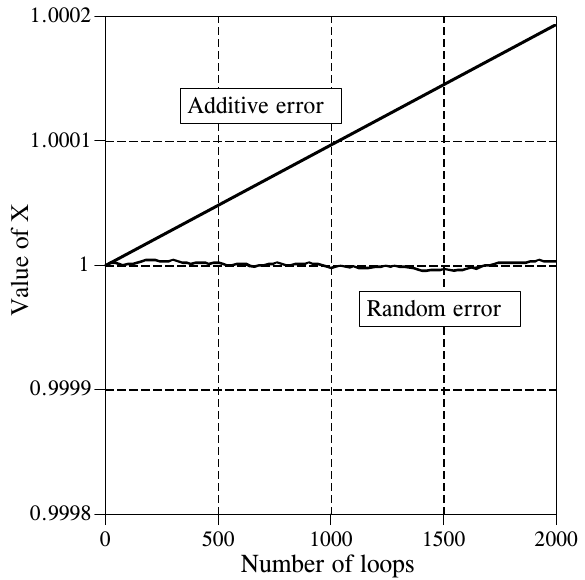
\includegraphics[width=0.487\linewidth,height=0.8\textheight,keepaspectratio]{assets/ch04/fig4-04.png}
\caption*{\textbf{图 4-4　浮点变量中舍入误差的累积。} 这些曲线由表 4-1
的程序生成。当一个浮点变量反复参与算术运算时，累积的舍入误差会使变量的值漂移。如果误差有正有负，值会随机地增减。如果舍入误差主要是同一个符号，值的变化会快得多、一致得多。
（Additive error = 累加误差，Random error = 随机误差，Value of X = X
的值，Number of loops = 循环次数。）}
\end{figure}

图 4-4 显示了这个示例程序中变量 X
的值是怎样漂移的。一个明显值得担心的地方是：累加误差比随机误差糟糕得多。这是因为随机误差往往会互相抵消，而累加误差只会不断积累。累加误差大约等于单次运算的舍入误差乘以运算的总次数。相比之下，随机误差只按运算次数的平方根增长。如这个例子所示，对常见的
DSP 算法来说，累加误差可能比随机误差糟糕几百倍。

遗憾的是，几乎不可能控制或预测某个特定算法会呈现这两种行为中的哪一种。例如，表
4-1
的程序产生的是累加误差。只要对加减的数稍作修改，就能把它变成随机误差。具体来说，图
4-4 中的随机误差曲线是这样生成的：定义 A = EXP(RND) 和 B =
EXP(RND)，而不是 A = RND 和 B = RND。这样 A 和 B 就不再是 0 到 1
之间均匀分布的随机数，而变成 1 到 2.718
之间按指数分布的值。即使这么小的改动，也足以切换误差累积的模式。

既然我们无法控制舍入误差以哪种方式累积，就要记住最坏的情况。预计每个单精度数都会有大约四千万分之一的误差，再乘以它经历过的运算次数。这基于两个假设：误差是累加的，单次运算的平均误差是四分之一个量化电平。按同样的分析，每个双精度数都有大约四亿亿分之一（四十千万亿分之一）的误差，乘以运算次数。

\textbf{表 4-2　用浮点变量和整数变量控制循环的比较。}
左边的程序用浮点变量 X 控制 FOR-NEXT 循环。到程序结束时累积了 0.000133
的舍入误差，导致最后一个循环值 X = 10.0
被漏掉。相比之下，右边的程序用整数 I\%
作为循环索引。这提供了完美的精度，保证执行正确的循环次数。

左：用浮点数控制循环

\begin{Shaded}
\begin{Highlighting}[]
\NormalTok{100 \textquotesingle{}Floating Point Loop Control}
\NormalTok{110 FOR X = 0 TO 10 STEP 0.01}
\NormalTok{120   PRINT X}
\NormalTok{130 NEXT X}
\end{Highlighting}
\end{Shaded}

程序输出：

\begin{Shaded}
\begin{Highlighting}[]
\NormalTok{0.00}
\NormalTok{0.01}
\NormalTok{0.02}
\NormalTok{0.03}
\NormalTok{ ⋮}
\NormalTok{9.960132}
\NormalTok{9.970133}
\NormalTok{9.980133}
\NormalTok{9.990133}
\end{Highlighting}
\end{Shaded}

右：用整数控制循环

\begin{Shaded}
\begin{Highlighting}[]
\NormalTok{100 \textquotesingle{}Integer Loop Control}
\NormalTok{110 FOR I\% = 0 TO 1000}
\NormalTok{120   X = I\%/100}
\NormalTok{130   PRINT X}
\NormalTok{140 NEXT I\%}
\end{Highlighting}
\end{Shaded}

程序输出：

\begin{Shaded}
\begin{Highlighting}[]
\NormalTok{0.00}
\NormalTok{0.01}
\NormalTok{0.02}
\NormalTok{0.03}
\NormalTok{ ⋮}
\NormalTok{9.96}
\NormalTok{9.97}
\NormalTok{9.98}
\NormalTok{9.99}
\NormalTok{10.00}
\end{Highlighting}
\end{Shaded}

\textbf{C 实现}（两段程序合在一个文件里，完整可编译版本见
\texttt{c/table4-2\_loop\_control.c}）：

\begin{Shaded}
\begin{Highlighting}[]
\CommentTok{/* 表 4{-}2  用浮点数和整数控制循环的对比}
\CommentTok{ * 两段都想打印 0 到 10 之间等间距的 1001 个数；为便于对照，}
\CommentTok{ * 只打印每段的前 4 个和后 4 个值，以及实际循环次数。 */}
\PreprocessorTok{\#include }\ImportTok{\textless{}stdio.h\textgreater{}}

\DataTypeTok{static} \DataTypeTok{void}\NormalTok{ show}\OperatorTok{(}\DataTypeTok{int}\NormalTok{ k}\OperatorTok{,} \DataTypeTok{float}\NormalTok{ x}\OperatorTok{,} \DataTypeTok{int}\NormalTok{ count}\OperatorTok{)}
\OperatorTok{\{}
    \ControlFlowTok{if} \OperatorTok{(}\NormalTok{k }\OperatorTok{\textless{}} \DecValTok{4} \OperatorTok{||}\NormalTok{ k }\OperatorTok{\textgreater{}=}\NormalTok{ count }\OperatorTok{{-}} \DecValTok{4}\OperatorTok{)}\NormalTok{ printf}\OperatorTok{(}\StringTok{"  }\SpecialCharTok{\%.6f\textbackslash{}n}\StringTok{"}\OperatorTok{,}\NormalTok{ x}\OperatorTok{);}
    \ControlFlowTok{else} \ControlFlowTok{if} \OperatorTok{(}\NormalTok{k }\OperatorTok{==} \DecValTok{4}\OperatorTok{)}\NormalTok{ printf}\OperatorTok{(}\StringTok{"  ...}\SpecialCharTok{\textbackslash{}n}\StringTok{"}\OperatorTok{);}
\OperatorTok{\}}

\DataTypeTok{int}\NormalTok{ main}\OperatorTok{(}\DataTypeTok{void}\OperatorTok{)}
\OperatorTok{\{}
    \CommentTok{/* 左：110 FOR X = 0 TO 10 STEP 0.01，X 是单精度浮点数 */}
    \DataTypeTok{int}\NormalTok{ count }\OperatorTok{=} \DecValTok{0}\OperatorTok{;}
    \ControlFlowTok{for} \OperatorTok{(}\DataTypeTok{float}\NormalTok{ x }\OperatorTok{=} \FloatTok{0.0}\BuiltInTok{f}\OperatorTok{;}\NormalTok{ x }\OperatorTok{\textless{}=} \FloatTok{10.0}\BuiltInTok{f}\OperatorTok{;}\NormalTok{ x }\OperatorTok{+=} \FloatTok{0.01}\BuiltInTok{f}\OperatorTok{)}\NormalTok{ count}\OperatorTok{++;}
\NormalTok{    printf}\OperatorTok{(}\StringTok{"浮点数控制循环：共执行 }\SpecialCharTok{\%d}\StringTok{ 次（应为 1001）}\SpecialCharTok{\textbackslash{}n}\StringTok{"}\OperatorTok{,}\NormalTok{ count}\OperatorTok{);}
    \DataTypeTok{int}\NormalTok{ k }\OperatorTok{=} \DecValTok{0}\OperatorTok{;}
    \ControlFlowTok{for} \OperatorTok{(}\DataTypeTok{float}\NormalTok{ x }\OperatorTok{=} \FloatTok{0.0}\BuiltInTok{f}\OperatorTok{;}\NormalTok{ x }\OperatorTok{\textless{}=} \FloatTok{10.0}\BuiltInTok{f}\OperatorTok{;}\NormalTok{ x }\OperatorTok{+=} \FloatTok{0.01}\BuiltInTok{f}\OperatorTok{)}\NormalTok{ show}\OperatorTok{(}\NormalTok{k}\OperatorTok{++,}\NormalTok{ x}\OperatorTok{,}\NormalTok{ count}\OperatorTok{);}

    \CommentTok{/* 右：110 FOR I\% = 0 TO 1000，120 X = I\%/100 */}
\NormalTok{    printf}\OperatorTok{(}\StringTok{"整数控制循环：共执行 1001 次}\SpecialCharTok{\textbackslash{}n}\StringTok{"}\OperatorTok{);}
    \ControlFlowTok{for} \OperatorTok{(}\DataTypeTok{int}\NormalTok{ i }\OperatorTok{=} \DecValTok{0}\OperatorTok{;}\NormalTok{ i }\OperatorTok{\textless{}=} \DecValTok{1000}\OperatorTok{;}\NormalTok{ i}\OperatorTok{++)} \OperatorTok{\{}
        \DataTypeTok{float}\NormalTok{ x }\OperatorTok{=}\NormalTok{ i }\OperatorTok{/} \FloatTok{100.0}\BuiltInTok{f}\OperatorTok{;}
\NormalTok{        show}\OperatorTok{(}\NormalTok{i}\OperatorTok{,}\NormalTok{ x}\OperatorTok{,} \DecValTok{1001}\OperatorTok{);}
    \OperatorTok{\}}
    \ControlFlowTok{return} \DecValTok{0}\OperatorTok{;}
\OperatorTok{\}}
\end{Highlighting}
\end{Shaded}

实测输出和原书一致：浮点数控制的循环只执行了 1000 次，最后几个值是
9.960133、9.970133、9.980133、9.990133，10.00 被漏掉；整数控制的循环执行
1001 次，最后一个值是 10.000000。

表 4-2
说明了舍入误差带来的一个特别恼人的问题。表中两个程序做的是同一件事：打印
0 到 10 之间等间距的 1001 个数。左边的程序用浮点变量 X
作循环索引。执行循环时，计算机先把索引变量设为循环的起始值（本例中为
0）。每次循环结束时，把步长（这里是
0.01）加到索引上。然后做一个判断：还需要更多次循环，还是循环已经完成？当计算机发现索引的值大于终止值（本例中为
10.0）时，循环结束。从生成的输出可以看出，加法中的舍入误差使 X
的值在循环过程中累积了明显的偏差。事实上，累积的误差导致最后一次循环没有执行。在最后一次循环时，X
本该是 10.0，误差却让 X 的最后一个值变成了 10.000133。由于 X
大于终止值，计算机以为活干完了，循环就提前结束了。漏掉最后一个值，是许多计算机程序中常见的
bug。

相比之下，右边的程序用整数变量 I\%
控制循环。两个整数相加、相减或相乘，结果总是另一个整数。这意味着定点表示在这些运算中完全没有舍入误差。整数非常适合控制循环，也适合其他要经历多次数学运算的变量。最后一次循环保证会被执行！除非有充分的理由不这么做，循环索引和计数器一律用整数。

如果你一定要用浮点变量作循环索引，尽量用 2 的幂次分数（比如
1/2、1/4、3/8、27/16），而不要用 10 的幂次分数（比如 0.1、0.6、1.4、2.3
等）。例如，用 \texttt{FOR\ X\ =\ 1\ TO\ 10\ STEP\ 0.125} 比用
\texttt{FOR\ X\ =\ 1\ TO\ 10\ STEP\ 0.1}
好。这样索引总能有精确的二进制表示，从而减少舍入误差。例如，十进制数
1.125
可以在二进制中精确表示：\(1.001000000000000000000000 \times 2^0\)。相比之下，十进制数
1.1 落在两个浮点数之间：1.0999999046 和 1.1000000238（二进制分别是
\(1.00011001100110011001100 \times 2^0\) 和
\(1.00011001100110011001101 \times 2^0\)）。这导致程序中每次遇到 1.1
都会带有固有误差。

有一个值得记住的事实：单精度浮点数对 ±1680 万（准确地说是
\(\pm 2^{24}\)）以内的每个整数都有精确的二进制表示。超过这个值，电平之间的间隙就大于
1，有些整数值就会被跳过。这使得（±1680
万以内的）浮点整数之间的加、减、乘没有舍入误差。

\section{运行速度：编程语言}

DSP
编程大致可以分为三个复杂层次：汇编(Assembly)、编译型(Compiled)和专用应用(Application
Specific)。要理解这三者的区别，得从数字电子学最基础的东西讲起。所有微处理器都围绕一组内部二进制寄存器(register)构建，即一组能存储一串
0 和 1 的触发器。例如，原始 IBM PC 的核心------8088
微处理器------有四个通用寄存器，每个 16 位，名字分别是 AX、BX、CX 和
DX。另外还有九个特殊用途的寄存器：SI、DI、SP、BP、CS、DS、SS、ES 和
IP。例如，IP 即指令指针(Instruction
Pointer)，记录下一条指令在内存中的位置。

假设你写一个程序，把 1234 和 4321 两个数相加。程序开始时，IP
存放着一段内存的地址，这段内存里是一串 0 和 1 的模式，如表 4-3
所示。虽然在大多数人看来毫无意义，这串 0 和 1
却包含了完成任务所需的全部命令和数据。例如，当微处理器遇到比特模式
00000011 11000011 时，它把它解释为一条命令：取出 BX 寄存器中存储的 16
位，以二进制方式加到 AX 寄存器中存储的 16 位上，并把结果存入 AX
寄存器。这个层次的编程叫机器码(machine
code)，只比直接摆弄电子电路高一丁点。

\textbf{表 4-3　把 1234 和 4321 相加的机器码程序。}
这是最低层次的编程：直接操纵数字电路。（右栏接续左栏。）

\begin{Shaded}
\begin{Highlighting}[]
\NormalTok{10111001    00000000}
\NormalTok{11010010    10100001}
\NormalTok{00000100    00000000}
\NormalTok{10001001    00000000}
\NormalTok{00001110    10001011}
\NormalTok{00000000    00011110}
\NormalTok{00000000    00000010}
\NormalTok{10111001    00000000}
\NormalTok{11100001    00000011}
\NormalTok{00010000    11000011}
\NormalTok{10001001    10100011}
\NormalTok{00001110    00000100}
\NormalTok{00000010    00000000}
\end{Highlighting}
\end{Shaded}

用二进制干活迟早会把最有耐心的工程师逼疯，所以这些 0 和 1
的模式按它们执行的功能被起了名字。这个层次的编程叫汇编(assembly)，表 4-4
是一个例子。汇编程序虽然容易理解得多，但本质上和用机器码编程是一样的，因为程序命令和微处理器中执行的动作是一一对应的。例如：\texttt{ADD\ AX,\ BX}
翻译成 00000011 11000011。一个叫汇编器(assembler)的程序，把表 4-4
中的汇编代码（叫源代码(source code)）转换成表 4-3 那样的 0 和 1
模式（叫目标代码(object code)或可执行代码(executable
code)）。这种可执行代码可以直接在微处理器上运行。显然，汇编编程要求你对打算使用的那款微处理器的内部结构有深入的了解。

\textbf{表 4-4　把 1234 和 4321 相加的汇编程序。}
汇编器是把汇编程序转换成机器码的程序。（注释已译成中文）

\begin{Shaded}
\begin{Highlighting}[]
\BuiltInTok{MOV} \KeywordTok{CX}\OperatorTok{,}\DecValTok{1234}      \CommentTok{;把 1234 存入寄存器 CX，然后}
\BuiltInTok{MOV} \KeywordTok{DS}\OperatorTok{:[}\DecValTok{0}\OperatorTok{],}\KeywordTok{CX}    \CommentTok{;把它转存到内存地址 DS:[0]}

\BuiltInTok{MOV} \KeywordTok{CX}\OperatorTok{,}\DecValTok{4321}      \CommentTok{;把 4321 存入寄存器 CX，然后}
\BuiltInTok{MOV} \KeywordTok{DS}\OperatorTok{:[}\DecValTok{2}\OperatorTok{],}\KeywordTok{CX}    \CommentTok{;把它转存到内存地址 DS:[0]}

\BuiltInTok{MOV} \KeywordTok{AX}\OperatorTok{,}\KeywordTok{DS}\OperatorTok{:[}\DecValTok{0}\OperatorTok{]}    \CommentTok{;把存放在内存 DS:[0] 和 DS:[2]}
\BuiltInTok{MOV} \KeywordTok{BX}\OperatorTok{,}\KeywordTok{DS}\OperatorTok{:[}\DecValTok{2}\OperatorTok{]}    \CommentTok{;的变量分别移入 AX 和 BX}
\BuiltInTok{ADD} \KeywordTok{AX}\OperatorTok{,}\KeywordTok{BX}        \CommentTok{;AX 与 BX 相加，和存入 AX}
\BuiltInTok{MOV} \KeywordTok{DS}\OperatorTok{:[}\DecValTok{4}\OperatorTok{],}\KeywordTok{AX}    \CommentTok{;把和移到内存 DS:[4]}
\end{Highlighting}
\end{Shaded}

\begin{quote}
译注：第 4 行注释原书写的是 DS:{[}0{]}，按指令应为
DS:{[}2{]}，这里保留原文。
\end{quote}

汇编编程直接操纵数字电路：寄存器、内存地址、状态位等。再往上一个层次，可以操纵抽象的变量，完全不涉及具体的硬件。这些叫编译型语言或高级语言(high-level
languages)。常用的有十来种，比如
C、BASIC、FORTRAN、PASCAL、APL、COBOL、LISP 等。表 4-5 是一个把 1234 和
4321 相加的 BASIC 程序。程序员只知道变量 A、B 和 C，对硬件一无所知。

\textbf{表 4-5　把 1234 和 4321 相加的 BASIC 程序。}
编译器是把这类高级源代码转换成机器码的程序。

\begin{Shaded}
\begin{Highlighting}[]
\NormalTok{100 A = 1234}
\NormalTok{110 B = 4321}
\NormalTok{120 C = A+B}
\NormalTok{130 END}
\end{Highlighting}
\end{Shaded}

\textbf{C 实现}（完整可编译版本见 \texttt{c/table4-5\_add.c}）：

\begin{Shaded}
\begin{Highlighting}[]
\CommentTok{/* 表 4{-}5  把 1234 和 4321 相加 */}
\PreprocessorTok{\#include }\ImportTok{\textless{}stdio.h\textgreater{}}

\DataTypeTok{int}\NormalTok{ main}\OperatorTok{(}\DataTypeTok{void}\OperatorTok{)}
\OperatorTok{\{}
    \DataTypeTok{float}\NormalTok{ a }\OperatorTok{=} \DecValTok{1234}\OperatorTok{;}                 \CommentTok{/* 100 A = 1234（BASIC 默认单精度浮点） */}
    \DataTypeTok{float}\NormalTok{ b }\OperatorTok{=} \DecValTok{4321}\OperatorTok{;}                 \CommentTok{/* 110 B = 4321 */}
    \DataTypeTok{float}\NormalTok{ c }\OperatorTok{=}\NormalTok{ a }\OperatorTok{+}\NormalTok{ b}\OperatorTok{;}                \CommentTok{/* 120 C = A+B */}
\NormalTok{    printf}\OperatorTok{(}\StringTok{"C = }\SpecialCharTok{\%.0f\textbackslash{}n}\StringTok{"}\OperatorTok{,}\NormalTok{ c}\OperatorTok{);}
    \ControlFlowTok{return} \DecValTok{0}\OperatorTok{;}
\OperatorTok{\}}
\end{Highlighting}
\end{Shaded}

表 4-3 的机器码和表 4-4 的汇编针对的是 1981 年的 8088 处理器，没有对应的
C 版本。想看 C 编译器把上面几行变成了什么汇编，可以在 \texttt{c/}
目录下运行 \texttt{cc\ -O0\ -S\ -o\ -\ table4-5\_add.c}。在 Apple
Silicon Mac 上，你会看到 ARM64 指令，而不是书里的 8088
指令（比如浮点加法是 \texttt{fadd}，而不是 \texttt{ADD\ AX,BX}）。

一个叫编译器(compiler)的程序把高级源代码直接转换成机器码。这要求编译器给引用到的每个抽象变量分配硬件内存地址。例如，编译器第一次在表
4-5 中遇到变量 A（第 100
行）时，它明白程序员用这个符号表示一个单精度浮点变量。相应地，编译器指定四个字节的内存，专门用来存放这个变量的值。此后程序中每次出现
A，计算机都知道要按需更新这四个字节的值。编译器还会把复杂的数学表达式，比如
Y =
LOG(XCOS(Z))，拆成更基本的算术运算。微处理器只会加、减、乘、除，更复杂的运算都必须分解成这四种基本运算的一系列组合来完成。

高级语言把程序员和硬件隔离开。这让编程容易得多，也让源代码可以在不同类型的微处理器之间移植。最重要的是，使用编译型语言的程序员完全不需要了解计算机的内部运作。另一位程序员------编写编译器的那位------承担了这份责任。

大多数编译器在程序执行之前，先把整个程序转换成机器码。一个例外是一类叫解释器(interpreter)的编译器，解释型
BASIC
是最常见的例子。解释器把一行源代码转换成机器码，执行这段机器码，再处理下一行源代码。这为简单程序提供了一个交互式环境，尽管执行速度极慢（大约慢
100 倍）。

最高层次的编程出现在 DSP
应用软件包中。它们形式多样，通常是为支持特定硬件而提供的。假设你买了一款新开发的
DSP 微处理器，要嵌入到你当前的项目中。这些器件往往内置了许多 DSP
功能：模拟输入、模拟输出、数字
I/O、抗混叠和重建滤波器等。问题是：怎么给它编程？最坏的情况，厂商给你一个汇编器，指望你去学这个器件的内部架构。更典型的情况，厂商会提供一个
C 编译器，让你编程时不必操心微处理器实际上怎样运作。

最好的情况，厂商会提供一个功能完善的软件包来帮助编程：算法库、预先写好的
I/O
例程、调试工具等。你也许只需在一个易用的图形界面上把图标连起来，就能构成想要的系统。你操纵的东西是信号通路、处理信号的算法、模拟
I/O
参数等。对设计满意后，它会被转换成合适的机器码，在硬件上执行。其他类型的应用软件包用于图像处理、频谱分析、仪器与控制、数字滤波器设计等。这就是未来的样子。

这三个层次之间的界限可能很模糊。例如，大多数编译型语言都允许你直接操纵硬件。同样，一门配有丰富
DSP
函数库的高级语言，已经非常接近应用软件包了。这三个分类的意义在于让你明白自己在操纵什么：(1)
硬件，(2) 抽象变量，还是 (3) 整个过程和算法。

这些分类背后还有另一个重要概念。使用高级语言时，你依赖的是编写编译器的程序员，指望他们懂得操纵硬件的最佳技术。同样，使用应用软件包时，你依赖的是编写软件包的程序员，指望他们懂得最佳的
DSP
技术。麻烦就在这里：这些程序员从没见过你正在处理的具体问题。因此，他们不一定总能给你最优的解决方案。你在越高的层次上工作，就越要预料到最终的机器码在内存使用、速度和精度方面效率越低。

你应该用哪种编程语言？这取决于你是谁、打算做什么。大多数计算机科学家和程序员用
C（或更先进的 C++）。强大、灵活、模块化，C 样样都有。C
如此流行，以至于问题变成了：为什么有人会用 C 以外的语言来编写 DSP
应用？我想到三个答案。第一，DSP
发展得太快，有些组织和个人还困在其他语言（比如 FORTRAN 和
PASCAL）的模式里。军方和政府机构尤其如此，它们是出了名的改变缓慢。第二，有些应用要求极致的效率，只有汇编编程才能达到。这属于「多下很多功夫，换来快一点点」的类型。第三，C
不是一门特别容易掌握的语言，对兼职程序员来说尤其如此。这包括很多偶尔需要用
DSP 技术辅助研究或设计工作的工程师和科学家。这群人常常因为 BASIC
简单而选择它。

为什么本书选择 BASIC？本书讲的是算法，不是编程风格。你应该专注于 DSP
技术，而不是被某门语言的怪癖分心。例如，本书所有程序都有行号。这样描述程序的运作就很容易：「第
100 行做这个，第 110
行做那个」等等。当然，你在实际程序中大概永远不会用行号。关键在于，学 DSP
和用 DSP 的需求不同。市面上有许多书为 DSP
算法提供了精致的源代码。如果你只是想找现成的代码复制到自己的程序里，那你找错地方了。

比较硬件或软件的运行速度是一件吃力不讨好的事：无论结果如何，输的一方都会哭喊比赛不公平！喜欢高级语言的程序员（比如传统的计算机科学家）会争辩说，汇编只比编译代码快
50\%，麻烦却多五倍。喜欢汇编的人（通常是科学家和硬件工程师）则会说反过来：汇编快五倍，难度却只多
50\%。和大多数争论一样，双方都能拿出有选择性的数据来支持自己的说法。

作为经验法则，预计用汇编写的子程序比相应的高级语言程序快 1.5 到 3.0
倍。要知道确切的数值，唯一的办法是写出代码，做速度测试。个人计算机的速度每年大约提高
40\%，所以用汇编写一个例程，大约相当于硬件技术跃进两年。

大多数专业程序员对使用汇编的想法相当反感，你要是建议用
BASIC，他们会作呕。他们的理由很简单：汇编和 BASIC
不鼓励良好的软件实践。好的代码应该是可移植的（能从一种计算机移到另一种计算机）、模块化的（分解成定义良好的子程序结构）、易于理解的（大量注释和描述性的变量名）。汇编和
BASIC 结构薄弱，很难达到这些标准。更糟的是，被汇编和 BASIC
吸引的人，往往很少受过关于正确软件结构和文档编写的正规训练。

汇编爱好者对这种攻击也有自己的妙语回击。假设你用 C
写了一个程序，你的竞争对手用汇编写了同样的程序。最终用户的第一印象会是：你的程序是垃圾，因为它慢一倍。没有人建议你用汇编写大型程序，只是程序中需要快速执行的那些部分。例如，DSP
软件库中的许多函数都是用汇编写的，再从用 C
写的大程序中调用。即使最坚定的软件纯粹主义者也会用汇编代码，只要不用他们自己写就行。

\section{运行速度：硬件}

计算能力增长得如此之快，任何关于这个主题的书在出版前就过时了。这是作者的噩梦！最初的
IBM PC 于 1981 年推出，基于时钟频率 4.77 MHz、数据总线 8 位的 8088
微处理器。此后每隔 3～4 年就推出新一代个人计算机：8088 \dspsym{→} 80286
\dspsym{→} 80386 \dspsym{→} 80486 \dspsym{→}
80586（Pentium，奔腾）。每一代新系统的计算速度都比上一代提高约五倍。到
1996 年，时钟频率已提高到 200 MHz，数据总线增加到 32
位。加上其他改进，短短 15 年里计算能力提高了近一千倍！你应该预计接下来
15 年还会再提高一千倍。

在这个瞬息万变的领域，获取最新信息的唯一途径就是直接来自厂商：广告、规格书、价目表等。别指望从书里找性能数据，去看杂志和你每天的报纸。预计原始计算速度每两年会翻一番以上。只了解当前的计算机性能状况是不够的，你需要理解并跟踪它是怎样演进的。

记住这一点，我们就可以概览一下运行速度是怎样受计算机硬件限制的。由于计算机由许多子系统组成，执行某项任务所需的时间取决于两个主要因素：(1)
各个子系统的速度；(2) 在这些模块之间传输数据所需的时间。图 4-5
是典型个人计算机中最重要的限速部件的简化示意图。中央处理器(CPU, Central
Processing Unit)是系统的心脏。如前所述，它由十来个寄存器组成，每个能存放
32 位（在当代个人计算机中）。CPU
中还包含执行基本操作所需的数字电路，比如搬移比特和定点运算。

更复杂的数学运算，是通过把数据传给一个叫数学协处理器(math
coprocessor，也叫算术逻辑单元(ALU, arithmetic logic
unit))的专用硬件电路来处理的。数学协处理器可能和 CPU
在同一块芯片上，也可能是一个单独的电子器件。例如，两个浮点数相加，需要
CPU 把 8 个字节（每个数 4
个字节）以及几个描述如何处理这些数据的字节传给数学协处理器。经过短暂的计算后，数学协处理器把四个字节传回
CPU，里面就是作为和的那个浮点数。最便宜的计算机系统没有数学协处理器，或者只把它作为选配件。例如，80486DX
微处理器内置了数学协处理器，而 80486SX
没有。这些性能较低的系统用软件代替硬件：每个数学函数都被分解成 CPU
能直接处理的基本二进制运算。虽然结果相同，执行时间却慢得多，比如慢 10 到
20 倍。

\begin{figure}[htbp]
\centering
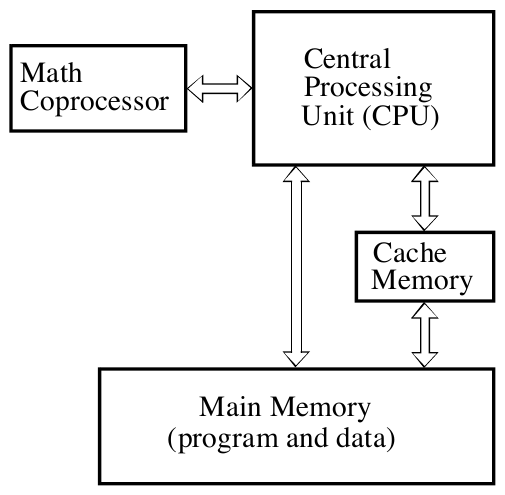
\includegraphics[width=0.421\linewidth,height=0.8\textheight,keepaspectratio]{assets/ch04/fig4-05.png}
\caption*{\textbf{图 4-5　典型计算机系统的架构。} 计算速度受以下因素限制：(1)
各个子系统的速度；(2) 数据在这些子系统之间传输的速率。 （Math
Coprocessor = 数学协处理器，Central Processing Unit (CPU) =
中央处理器，Cache Memory = 高速缓存，Main Memory (program and data) =
主存（存放程序和数据）。）}
\end{figure}

大多数个人计算机软件有没有数学协处理器都能用。做法是让编译器生成处理两种情况的机器码，全都存放在最终的可执行程序中。如果所用的计算机上有数学协处理器，就运行其中一段代码；没有的话，就用另一段代码。也可以让编译器只为其中一种情况生成代码。例如，你偶尔会遇到要求必须有数学协处理器的程序，在没有协处理器的计算机上运行就会崩溃。文字处理之类的应用通常不会从数学协处理器中获益，因为它们做的是在内存中搬移数据，而不是计算数学表达式。同样，涉及定点变量（整数）的计算也不受有无数学协处理器的影响，因为它们在
CPU 内部处理。另一方面，使用浮点计算的 DSP
和其他计算型程序，有无数学协处理器，执行速度可能相差一个数量级。

在大多数计算机系统中，CPU 和主存(main
memory)位于不同的芯片上。出于显而易见的原因，你希望主存非常大、非常快。可惜这会让内存非常贵。主存与
CPU 之间的数据传输，是一个非常常见的速度瓶颈。CPU
向主存索取某个内存地址上的二进制信息，然后必须等待接收。绕开这个问题的常用技术是使用高速缓存(memory
cache)。这是一小块非常快的内存，用作 CPU
和主存之间的缓冲区，典型容量是几百 KB。当 CPU
请求主存提供某个地址上的二进制数据时，高速数字电路会把主存中这个地址附近的一段内容复制到高速缓存里。下次
CPU
请求内存信息时，它很可能已经在高速缓存里了，取用就非常快。这是基于这样一个事实：程序往往会访问之前访问过的数据附近的内存位置。在典型的个人计算机应用中，加上高速缓存能把整体速度提高好几倍。高速缓存可能和
CPU 在同一块芯片上，也可能是一个外部电子器件。

子系统之间传输数据的速率，取决于提供了多少条并行数据线，以及每条线上数字信号能传递的最大速率。一般来说，在单块芯片内部传输数字数据，比在芯片之间传输快得多。同样，必须经过电连接器通到其他印刷电路板的数据通路（即总线(bus)结构）还要更慢。这是把尽可能多的电路塞进
CPU 的强大动力。

计算机速度的一个特别讨厌的问题是向后兼容(backward
compatibility)。当一家计算机公司推出新产品，比如一块数据采集卡或一个软件程序时，他们想卖进尽可能大的市场。这意味着它必须兼容当前在用的大多数计算机，而这些计算机可能横跨好几代技术。这常常把硬件或软件的性能限制在老旧得多的系统的水平上。例如，假设你买了一块插在
200 MHz 奔腾个人计算机总线上的 I/O
卡，它提供八条数字线，可以一次一个字节地收发数据。然后你写了一个汇编程序，在计算机和某个外部设备（比如一个科学实验装置或另一台计算机）之间快速传输数据。令你大吃一惊的是，最大数据传输速率只有大约每秒
100,000 字节，比微处理器的时钟频率慢一千多倍！罪魁祸首是 ISA
总线，一种向后兼容到 20 世纪 80 年代初计算机的技术。

表 4-6
给出了几代计算机的执行时间。显然，你应该把这些数据当作非常粗略的近似值。如果你想了解自己的系统，就在自己的系统上测量。这很简单：写一个循环，把某个运算执行一百万次，用手表计时看要多久。前三个系统
80286、80486 和奔腾，分别是 1986、1993 和 1996
年的标准台式个人计算机。第四个是 1994 年专为 DSP
任务设计的微处理器：德州仪器(Texas Instruments)的 TMS320C40。

\textbf{表 4-6　各种计算机实测的执行时间。} 时间单位为微秒。80286、80486
和奔腾是三代个人计算机，TMS320C40 是专为 DSP
任务设计的微处理器。所有个人计算机都配有数学协处理器。这些时间只能作为大致估计，你的计算机上的时间会因所用的具体硬件和软件而不同。

{\def\LTcaptype{none} % do not increment counter
\begin{longtable}[]{@{}
  >{\raggedright\arraybackslash}p{(\linewidth - 8\tabcolsep) * \real{0.1579}}
  >{\raggedleft\arraybackslash}p{(\linewidth - 8\tabcolsep) * \real{0.2105}}
  >{\raggedleft\arraybackslash}p{(\linewidth - 8\tabcolsep) * \real{0.2105}}
  >{\raggedleft\arraybackslash}p{(\linewidth - 8\tabcolsep) * \real{0.2105}}
  >{\raggedleft\arraybackslash}p{(\linewidth - 8\tabcolsep) * \real{0.2105}}@{}}
\toprule\noalign{}
\begin{minipage}[b]{\linewidth}\raggedright
运算
\end{minipage} & \begin{minipage}[b]{\linewidth}\raggedleft
80286（12 MHz）
\end{minipage} & \begin{minipage}[b]{\linewidth}\raggedleft
80486（33 MHz）
\end{minipage} & \begin{minipage}[b]{\linewidth}\raggedleft
奔腾（100 MHz）
\end{minipage} & \begin{minipage}[b]{\linewidth}\raggedleft
TMS320C40（40 MHz）
\end{minipage} \\
\midrule\noalign{}
\endhead
\bottomrule\noalign{}
\endlastfoot
\textbf{整数} & & & & \\
A\% = B\%+C\% & 1.6 & 0.12 & 0.04 & \\
A\% = B\%−C\% & 1.6 & 0.12 & 0.04 & \\
A\% = B\%×C\% & 2.7 & 0.59 & 0.13 & \\
A\% = B\%÷C\% & 64 & 9.2 & 1.5 & \\
\textbf{浮点数} & & & & \\
A = B+C & 33 & 2.5 & 0.50 & 0.10 \\
A = B−C & 35 & 2.5 & 0.50 & 0.10 \\
A = B×C & 35 & 2.5 & 0.50 & 0.10 \\
A = B÷C & 49 & 4.5 & 0.87 & 0.80 \\
A = SQR(B) & 45 & 5.3 & 1.3 & 0.90 \\
A = LOG(B) & 186 & 19 & 3.4 & 1.7 \\
A = EXP(B) & 246 & 25 & 5.5 & 1.7 \\
A = B\^{}C & 311 & 31 & 5.3 & 2.4 \\
A = SIN(B) & 262 & 30 & 6.6 & 1.1 \\
A = ARCTAN(B) & 168 & 21 & 4.4 & 2.2 \\
\end{longtable}
}

（原表中 TMS320C40 的整数运算一栏为空。）

奔腾比 80286 系统快，有四个原因：(1) 时钟频率更高；(2)
数据总线的线更多；(3) 加了高速缓存；(4)
内部设计更高效，每条指令需要的时钟周期更少。

如果说奔腾是凯迪拉克，那 TMS320C40
就是法拉利：不那么舒适，但速度快得惊人。这款芯片代表了专为缩短 DSP
算法执行时间而设计的一类微处理器。这一类中的其他型号有 Intel i860、AT\&T
DSP3210、Motorola DSP96002 和 Analog Devices ADSP-2171。它们常被称为 DSP
微处理器、数字信号处理器(Digital Signal Processor)和
RISC（精简指令集计算机，Reduced Instruction Set
Computer）。最后这个名字反映出：速度的提高来自提供给程序员的汇编级指令更少。相比之下，更传统的微处理器（比如奔腾）叫
CISC（复杂指令集计算机，Complex Instruction Set Computer）。

DSP
微处理器有两种用法：作为受更传统的计算机控制的从属模块，或者作为专用应用（比如蜂窝电话）中的嵌入式处理器。有些型号只能处理定点数，有些则能处理浮点数。为提高速度而采用的内部架构包括：(1)
片内有大量非常快的高速缓存；(2)
程序和数据使用分开的总线，可以同时访问两者（叫哈佛架构(Harvard
Architecture)）；(3) 微处理器内部直接集成了快速的数学运算硬件；(4)
流水线(pipeline)设计。

流水线架构把完成某项任务所需的硬件分成几个连续的阶段。例如，两个数相加可以分成三个流水线阶段完成。流水线的第一阶段只负责从内存中取出要相加的数。第二阶段唯一的任务是把两个数加起来。第三阶段只负责把结果存回内存。如果每个阶段都能在一个时钟周期内完成任务，整个过程需要三个时钟周期。流水线结构的关键特点是：前一个任务完成之前，就可以开始另一个任务。在这个例子中，第一个时钟周期结束、第一阶段一空闲下来，我们就可以开始另外两个数的加法。对于大量运算，系统的速度会被标称为每个时钟周期一次加法，尽管任意两个数相加都需要三个时钟周期才能完成。流水线对速度大有好处，但可能很难编程。算法必须允许在前面计算的结果还拿不到（因为还在流水线里）的情况下开始新的计算。

第 28 章和第 29 章会更详细地讨论 DSP
微处理器。它们是令人惊叹的器件，高性能、低成本，会把 DSP
带进广泛的消费类和科学应用中。这是将会塑造 21 世纪的技术之一。

\section{运行速度：编程技巧}

计算机硬件和编程语言虽然对最大化运行速度很重要，但不是你天天会更换的东西。相比之下，你怎样编程随时可以改变，而且会极大地影响程序的执行时间。这里有三条建议。

\textbf{第一，尽可能用整数代替浮点变量。}
传统的微处理器（比如个人计算机中用的那些）处理整数比处理浮点数快 10 到
20 倍。在没有数学协处理器的系统上，差距可能达到 200 比
1。一个例外是整数除法，它常常是先把值转换成浮点数再完成的。这使得它和其他整数运算相比慢得可怕。详见表
4-6。

\textbf{第二，避免使用 sin(x)、log(x)、\(y^x\) 这类函数。}
这些超越函数(transcendental
functions)是通过一系列加法、减法和乘法计算出来的。例如，麦克劳林幂级数(Maclaurin
power series)给出：

\textbf{公式 4-3　三个超越函数的麦克劳林幂级数展开。}
计算机就是这样计算这类函数的，这也是它们执行得很慢的原因。

\[
\sin(x) = x - \frac{x^3}{3!} + \frac{x^5}{5!} - \frac{x^7}{7!} + \frac{x^9}{9!} - \frac{x^{11}}{11!} + \cdots
\]

\[
\cos(x) = 1 - \frac{x^2}{2!} + \frac{x^4}{4!} - \frac{x^6}{6!} + \frac{x^8}{8!} - \frac{x^{10}}{10!} + \cdots
\]

\[
e^x = 1 + x + \frac{x^2}{2!} + \frac{x^3}{3!} + \frac{x^4}{4!} + \frac{x^5}{5!} + \cdots
\]

这些式子虽然无限长，但各项很快就小到可以忽略。例如：

\[
\sin(1) = 1 - 0.166666 + 0.008333 - 0.000198 + 0.000002 - \cdots
\]

计算这些函数所需的时间，大约是一次加法或乘法的十倍（见表
4-6）。可以用几种技巧绕开这些计算，比如：\(x^3 = x \cdot x \cdot x\)；当
x 很小时 \(\sin(x) \approx x\)；在已知其中一个值、需要求另一个值时，用
\(\sin(-x) = -\sin(x)\)，等等。大多数语言只提供少数几个超越函数，指望你用表
4-7 中的关系推导出其他函数。不出所料，这些推导出来的计算还要更慢。

\textbf{表 4-7　用较常用的函数计算很少用的函数。}
所有角度都以弧度为单位。ATN(X) 是反正切，LOG(X) 是自然对数，SGN(X) 是 X
的符号（即 X\textless0 时为 −1，X\textgreater0 时为 1），EXP(X) 是
\(e^X\)。

{\def\LTcaptype{none} % do not increment counter
\begin{longtable}[]{@{}ll@{}}
\toprule\noalign{}
函数 & 计算式 \\
\midrule\noalign{}
\endhead
\bottomrule\noalign{}
\endlastfoot
正割 Secant(X) & 1/COS(X) \\
余割 Cosecant(X) & 1/SIN(X) \\
余切 Cotangent(X) & 1/TAN(X) \\
反正弦 Arc Sine(X) & ATN(X/SQR(1-X*X)) \\
反余弦 Arc Cosine(X) & -ATN(X/SQR(1-X*X)) + PI/2 \\
反正割 Arc Secant(X) & ATN(SQR(X\emph{X-1)) + (SGN(X)-1) } PI/2 \\
反余割 Arc Cosecant(X) & ATN(1/SQR(X\emph{X-1)) + (SGN(X)-1) } PI/2 \\
反余切 Arc Cotangent(X) & -ATN(X) + PI/2 \\
双曲正弦 Hyperbolic Sine(X) & (EXP(X)-EXP(-X))/2 \\
双曲余弦 Hyperbolic Cosine(X) & (EXP(X)+EXP(-X))/2 \\
双曲正切 Hyperbolic Tangent(X) & (EXP(X)-EXP(-X))/(EXP(X)+EXP(-X)) \\
双曲正割 Hyperbolic Secant(X) & 1/双曲余弦 \\
双曲余割 Hyperbolic Cosecant(X) & 1/双曲正弦 \\
双曲余切 Hyperbolic Cotangent(X) & 1/双曲正切 \\
反双曲正弦 Arc Hyperbolic Sine(X) & LOG(X+SQR(X*X+1)) \\
反双曲余弦 Arc Hyperbolic Cosine(X) & LOG(X+SQR(X*X-1)) \\
反双曲正切 Arc Hyperbolic Tangent(X) & LOG((1+X)/(1-X))/2 \\
反双曲正割 Arc Hyperbolic Secant(X) & LOG((SQR(1-X*X)+1)/X) \\
反双曲余割 Arc Hyperbolic Cosecant(X) &
LOG(1+SGN(X)\emph{SQR(1+X}X))/X \\
反双曲余切 Arc Hyperbolic Cotangent(X) & LOG((X+1)/(X-1))/2 \\
LOG10(X) & LOG(X)/LOG(10) = 0.4342945 LOG(X) \\
PI & 4*ATN(1) = 3.141592653589794 \\
\end{longtable}
}

另一个办法是预先算好这些慢函数，把结果存进查找表(LUT, look-up
table)。例如，设想一个 8
比特数据采集系统，持续监测某个电阻两端的电压。如果关心的参数是电阻消耗的功率，就可以用测得的电压计算
\(P = V^2/R\)。更快的替代办法是：预先算好 256
种可能的电压测量值各自对应的功率，存进一个
LUT。系统运行时，测得的电压（0 到 255 之间的一个数字）就作为 LUT
的索引，查出对应的功率。查找表可能比直接计算快几百倍。

\textbf{第三，了解在你的具体系统上什么快、什么慢。}
这来自经验和测试，而且总会有意外。要特别留意图形命令和
I/O。处理这些需求通常有好几种方法，速度可能相差极大。例如，BASIC 命令
BLOAD
把一个数据文件直接传进一段内存。用循环一个字节一个字节地把同一个文件读进内存，可能慢
100 倍。再举一个例子，BASIC 命令 LINE
可以在显示屏上画一个彩色方框。一个像素一个像素地画同样的方框，也可能慢
100
倍。即使只是在循环里放一条打印语句（用来跟踪它在做什么），也可能让运算慢上几千倍！

% !TEX root = ../main.tex
% 本文件由 build-tex.sh 从 05-DSP指南-第5章中译.md 生成，改内容请改 md 后重新生成

\chapter{线性系统}\label{ch-05}

大多数 DSP
技术都基于一种叫叠加(superposition)的分而治之策略：把要处理的信号拆成简单的分量，逐个处理每个分量，再把结果合起来。这种方法有一个巨大的威力：把一个复杂的问题拆成许多简单的问题。叠加只能用于线性系统(linear
systems)，这个术语的意思是某些数学规则成立。幸运的是，科学和工程中遇到的大多数应用都属于这一类。本章介绍
DSP
的基础：系统是线性的意味着什么、把信号拆成更简单分量的各种方式，以及叠加怎样提供多种多样的信号处理技术。

\section{信号与系统}

信号(signal)描述的是一个参数怎样随另一个参数变化。例如，电子电路中随时间变化的电压，或图像中随距离变化的亮度。系统(system)是任何根据输入信号产生输出信号的过程。图
5-1
的框图说明了这一点。连续系统输入和输出连续信号，比如模拟电子电路。离散系统输入和输出离散信号，比如处理数组中所存数值的计算机程序。

给信号命名有几条规则。DSP
中并不总是遵守它们，但它们非常常见，你应该记住。数学本身已经够难了，没有清晰的记号会更难。第一，连续信号用圆括号，比如
x(t) 和 y(t)；离散信号用方括号，比如 x{[}n{]} 和
y{[}n{]}。第二，信号用小写字母。大写字母留给频域，后面的章节会讲到。第三，给信号起的名字通常能说明它代表的参数。例如，随时间变化的电压可以叫
v(t)，每天测一次的股价可以叫 p{[}d{]}。

\begin{figure}[htbp]
\centering
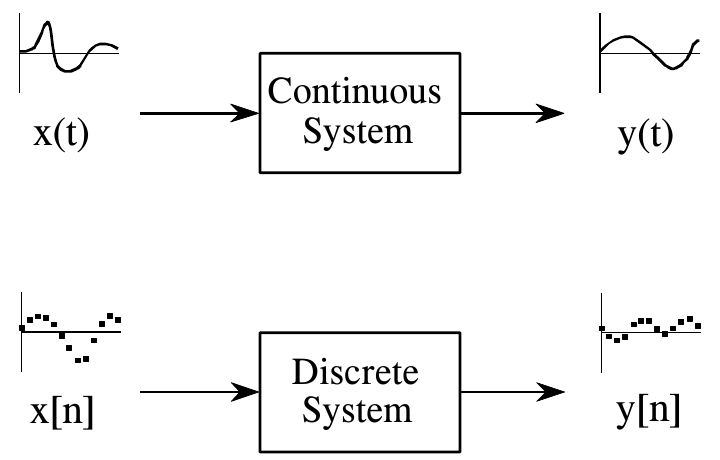
\includegraphics[width=0.600\linewidth,height=0.8\textheight,keepaspectratio]{assets/ch05/fig5-01.png}
\caption*{\textbf{图 5-1　信号与系统的术语。}
系统是任何根据输入信号生成输出信号的过程。连续信号通常用圆括号表示，离散信号用方括号表示。所有信号都用小写字母，大写字母留给频域（后面的章节介绍）。除非有更好的名字，输入信号叫
x(t) 或 x{[}n{]}，输出信号叫 y(t) 或 y{[}n{]}。 （Continuous System =
连续系统，Discrete System = 离散系统。）}
\end{figure}

讨论信号和系统时，常常并不知道所代表的具体参数是什么。这就像代数里用 x
和
y，而不赋予变量物理含义。由此引出给信号命名的第四条规则：如果没有更具描述性的名字，离散系统的输入信号通常叫
x{[}n{]}，输出信号叫 y{[}n{]}；连续系统则用 x(t) 和 y(t)。

想要理解一个系统的理由有很多。例如，你可能想设计一个系统来去除心电图中的噪声、让失焦的图像变清晰，或者去除录音中的回声。在另一些情况下，系统可能有某种失真或干扰效应，你需要刻画或测量它。例如，你对着电话说话时，期望对方听到的东西像你的声音。可惜传输线的输入信号很少和输出信号完全相同。如果你知道传输线（系统）是怎样改变信号的，也许就能补偿它的影响。还有一些情况，系统可能代表你想研究或分析的某个物理过程。雷达和声呐就是很好的例子。这些方法通过比较发射信号和反射信号，找出远处物体的特性。用系统理论的话说，问题就是找出那个把发射信号变成接收信号的系统。

乍一看，要理解世界上所有可能的系统，似乎是一项不可能完成的任务。幸运的是，大多数有用的系统都属于一个叫线性系统的类别。这个事实极其重要。没有线性系统的概念，我们将不得不逐个考察许多互不相关的系统各自的特性。有了这个概念，我们就能把注意力放在线性系统这一整类的共同特点上。我们的第一个任务，是弄清哪些性质使一个系统成为线性的，以及这些性质怎样对应到电子电路、软件和其他信号处理系统的日常概念上。

\section{线性的条件}

如果一个系统具有两个数学性质，就称它是线性的：齐次性(homogeneity)和可加性(additivity)。如果你能证明一个系统同时具有这两个性质，就证明了它是线性的。同样，如果你能证明一个系统不具有其中一个或两个性质，就证明了它不是线性的。第三个性质------平移不变性(shift
invariance)------不是线性的严格要求，但对大多数 DSP
技术来说是必不可少的。在 DSP
中看到「线性系统」这个词时，除非有理由认为不是，否则你应该假定它包含平移不变性。这三个性质构成了定义和使用线性系统理论的数学基础。本章后面我们会看一些更直观的理解线性的方式。现在先来过一遍这些正式的数学性质。

如图 5-2
所示，齐次性的意思是：输入信号幅度的变化，会导致输出信号幅度相应的变化。用数学语言说，如果输入信号
x{[}n{]} 产生输出信号 y{[}n{]}，那么对于任何输入信号和任何常数 k，输入 k
x{[}n{]} 都会产生输出 k y{[}n{]}。

\begin{figure}[htbp]
\centering
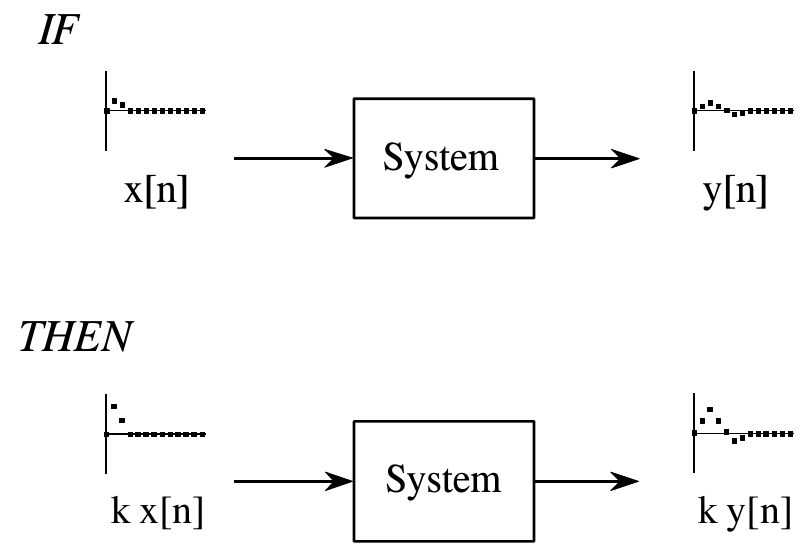
\includegraphics[width=0.675\linewidth,height=0.8\textheight,keepaspectratio]{assets/ch05/fig5-02.png}
\caption*{\textbf{图 5-2　齐次性的定义。}
如果输入的幅度变化在输出中引起相同的幅度变化，就称系统是齐次的。也就是说，如果
x{[}n{]} 产生 y{[}n{]}，那么对于任何信号 x{[}n{]} 和任何常数 k，k
x{[}n{]} 都产生 k y{[}n{]}。 （IF = 如果，THEN = 那么，System = 系统。）}
\end{figure}

一个简单的电阻就能很好地说明齐次和非齐次系统。如果系统的输入是电阻两端的电压
v(t)，输出是流过电阻的电流 i(t)，这个系统就是齐次的。欧姆定律(Ohm's
law)保证了这一点：电压增大或减小，电流就会相应地增大或减小。现在考虑另一个系统，输入信号仍是电阻两端的电压
v(t)，输出信号却是电阻消耗的功率
p(t)。由于功率与电压的平方成正比，输入信号增大到两倍，输出信号就增大到四倍。这个系统不是齐次的，因此不可能是线性的。

图 5-3 说明了可加性。考虑一个系统，输入 \(x_1[n]\) 产生输出
\(y_1[n]\)。再假设另一个输入 \(x_2[n]\) 产生另一个输出
\(y_2[n]\)。如果对于所有可能的输入信号，输入 \(x_1[n] + x_2[n]\)
都产生输出
\(y_1[n] + y_2[n]\)，就称这个系统是可加的。用文字说，在输入端相加的信号，在输出端产生的也是相加的信号。

\begin{figure}[htbp]
\centering
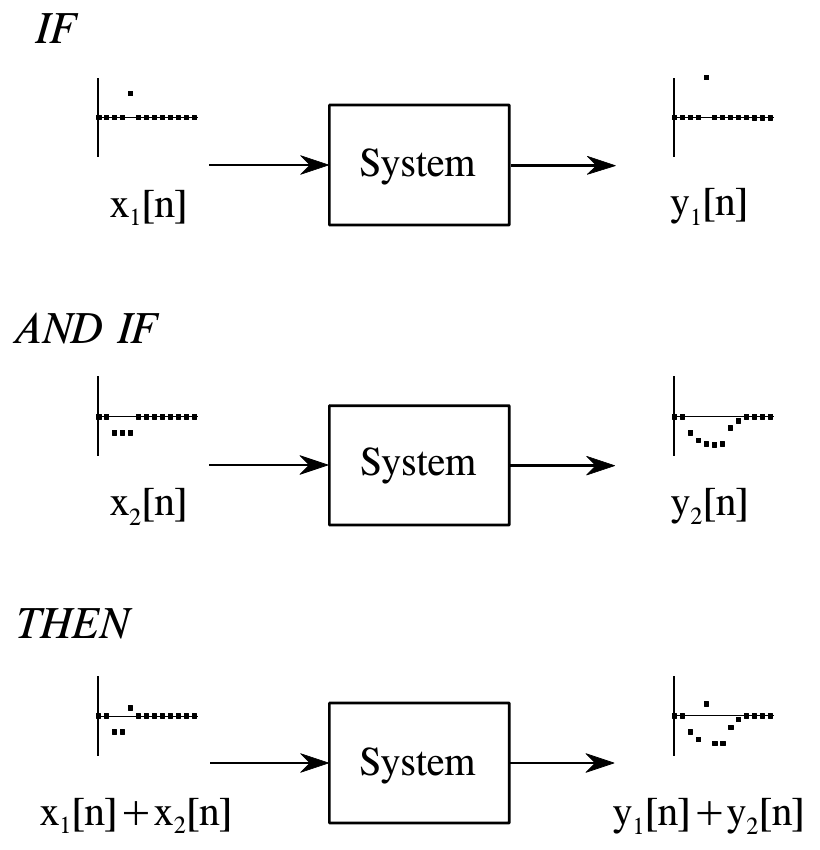
\includegraphics[width=0.683\linewidth,height=0.8\textheight,keepaspectratio]{assets/ch05/fig5-03.png}
\caption*{\textbf{图 5-3　可加性的定义。}
如果相加的信号通过系统时互不影响，就称系统是可加的。正式地说，如果
\(x_1[n]\) 产生 \(y_1[n]\)，并且 \(x_2[n]\) 产生 \(y_2[n]\)，那么
\(x_1[n]+x_2[n]\) 产生 \(y_1[n]+y_2[n]\)。 （IF = 如果，AND IF =
并且如果，THEN = 那么。原书图注最后一句误写成
\(y_2[n]+y_2[n]\)，这里按图改正。）}
\end{figure}

重点在于：相加的信号通过系统时互不影响。举个例子，想想和你的埃德娜姨妈、伯尼姨父打电话。埃德娜姨妈开始讲一个相当冗长的故事，说她今年的萝卜长得多好。背景里，伯尼姨父正冲着狗大吼，因为它在他最喜欢的椅子上闯了祸。两个人的声音信号相加后，通过电话网络以电子方式传输。由于这个系统是可加的，你听到的声音就是两个声音各自单独传输时听起来的样子之和。你听到的是埃德娜和伯尼，而不是一个叫「埃德娜伯尼」的怪物。

一个不可加电路的好例子，是无线电发射机中的混频级(mixer
stage)。这里有两个信号：一个是包含语音或音乐的音频信号，另一个是加到天线上就能在空间传播的载波(carrier
wave)。两个信号相加后送入一个非线性器件，比如 pn
结二极管。这使两个信号融合成第三个信号------一个能把信息传到很远的已调制无线电波。

如图 5-4
所示，平移不变性的意思是：输入信号的平移，只会导致输出信号同样的平移，别无其他。更正式地说，如果输入信号
x{[}n{]} 产生输出 y{[}n{]}，那么对于任何输入信号和任何常数 s，输入信号
x{[}n+s{]} 都产生输出
y{[}n+s{]}。要特别留意这个平移的数学写法，后面的章节会用到。给自变量 n
加上常数 s，就能让波形在水平方向上提前或延后。例如，s = 2
时，信号向左移两个采样；s = −2 时，信号向右移两个采样。

\begin{figure}[htbp]
\centering
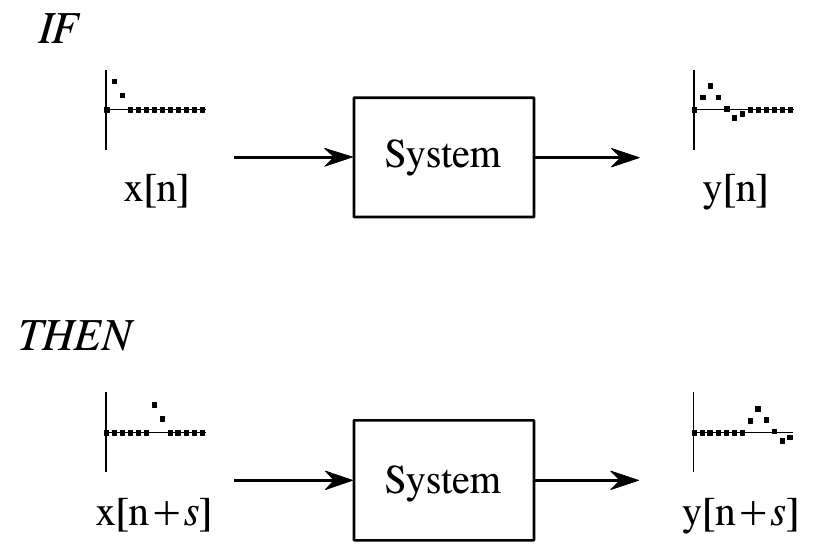
\includegraphics[width=0.683\linewidth,height=0.8\textheight,keepaspectratio]{assets/ch05/fig5-04.png}
\caption*{\textbf{图 5-4　平移不变性的定义。}
如果输入信号的平移在输出信号中引起相同的平移，就称系统是平移不变的。用数学语言说，如果
x{[}n{]} 产生 y{[}n{]}，那么对于任何信号 x{[}n{]} 和任何常数
s，x{[}n+s{]} 都产生 y{[}n+s{]}。}
\end{figure}

平移不变性很重要，因为它意味着系统的特性不随时间（或者不管自变量是什么）而变化。如果输入中的一个「哔」引起输出中的一个「啵」，你就可以确信，另一个「哔」会引起一个一模一样的「啵」。你遇到的大多数系统都是平移不变的。这是件幸事，因为运行中特性会变化的系统很难对付。例如，设想你设计了一个数字滤波器，用来补偿电话传输线的劣化效应。你的滤波器让声音听起来更自然、更容易听懂。让你大吃一惊的是，冬天来了，你发现电话线的特性随温度变了。你的补偿滤波器现在不匹配了，效果也不太好。这种情况可能需要一个更复杂的、能适应条件变化的算法。

为什么齐次性和可加性在线性中起关键作用，而平移不变性只是个附带的东西？这是因为线性是一个非常宽泛的概念，涵盖的远不止信号和系统。例如，设想一个农民卖橙子每箱
2 美元，卖苹果每箱 5 美元。如果他只卖橙子，10 箱收入 20 美元，20 箱收入
40 美元，这样的交易是齐次的。如果他卖 20 箱橙子和 10 箱苹果，收入是
\(20 \times \$2 + 10 \times \$5 = \$90\)。这和两样东西分开卖的收入相同，这样的交易是可加的。既齐次又可加，这种商品买卖就是一个线性过程。然而，这里不涉及信号，所以它不是一个系统，平移不变性也就没有意义。可以把平移不变性看作涉及信号和系统时，线性所需的一个附加方面。

\section{静态线性与正弦保真性}

齐次性、可加性和平移不变性很重要，因为它们为定义线性系统提供了数学基础。可惜单靠这些性质，大多数科学家和工程师并不能直观地感受到线性系统是怎么回事。静态线性(static
linearity)和正弦保真性(sinusoidal
fidelity)这两个性质在这里常常很有帮助。从数学角度看，它们并不特别重要，但它们关系到人们怎样思考和理解线性系统。你应该特别留意这一节。

静态线性定义的是：信号不变化时，即信号是直流或静态时，线性系统的反应。线性系统的静态响应非常简单：输出等于输入乘以一个常数。也就是说，把可能的输入值对应的输出值画成图，是一条通过原点的直线。图
5-5 展示了两个常见的线性系统：电阻的欧姆定律和弹簧的胡克定律(Hooke's
law)。作为对比，图 5-6 展示了两个非线性系统的静态关系：pn
结二极管和铁的磁特性。

\begin{figure}[htbp]
\centering
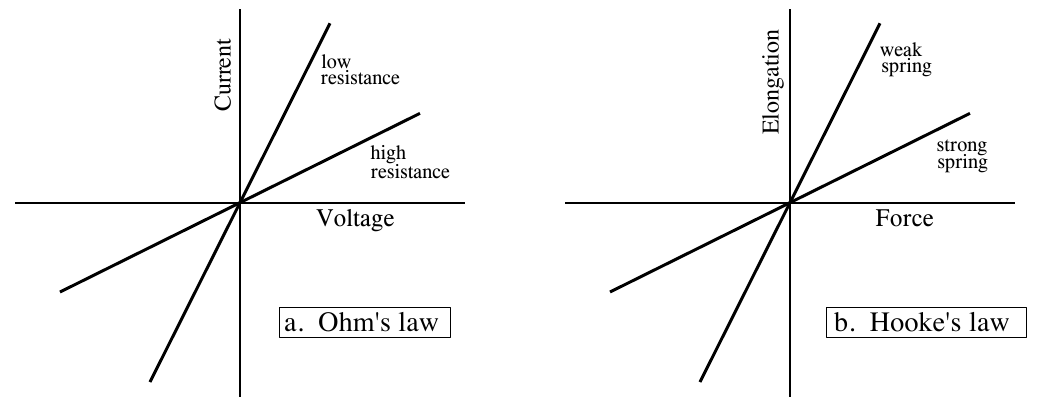
\includegraphics[width=0.867\linewidth,height=0.8\textheight,keepaspectratio]{assets/ch05/fig5-05.png}
\caption*{\textbf{图 5-5　静态线性的两个例子。} (a)
欧姆定律：流过电阻的电流等于电阻两端的电压除以电阻。(b)
胡克定律：弹簧的伸长量等于所施加的力乘以弹簧的刚度系数。 （a：Voltage =
电压，Current = 电流，low/high resistance = 小/大电阻；b：Force =
力，Elongation = 伸长量，weak/strong spring = 软/硬弹簧。）}
\end{figure}

所有线性系统都具有静态线性。反过来通常也成立，但并不总是成立。有些系统表现出静态线性，但对于变化的信号却不是线性的。不过，有一类非常常见的系统，单靠静态线性就能完全理解。在这类系统中，输入信号是静态的还是变化的都无所谓。它们叫无记忆系统(memoryless
systems)，因为输出只取决于输入的当前状态，而与输入的历史无关。例如，电阻中的瞬时电流只取决于它两端的瞬时电压，而与信号是怎样变成现在这个值的无关。如果一个系统具有静态线性，并且是无记忆的，那么它一定是线性的。这为理解（和证明）这些简单系统的线性提供了一个重要途径。

\begin{figure}[htbp]
\centering
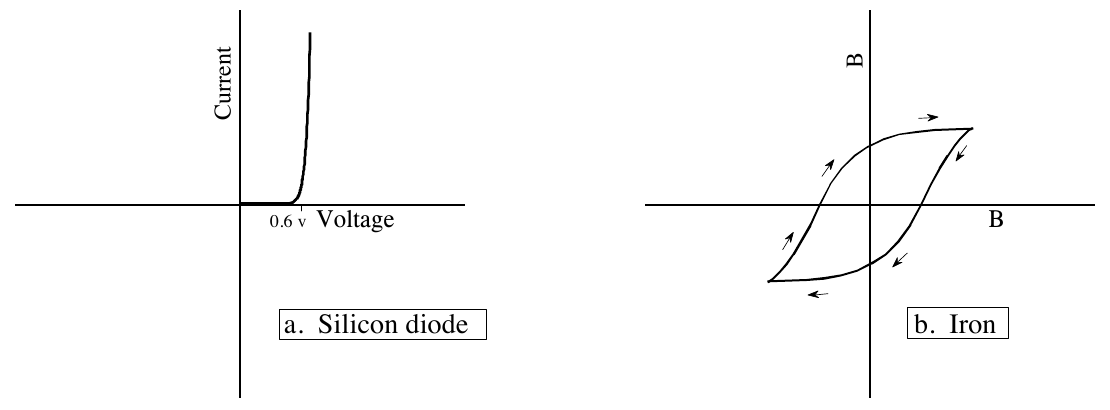
\includegraphics[width=0.925\linewidth,height=0.8\textheight,keepaspectratio]{assets/ch05/fig5-06.png}
\caption*{\textbf{图 5-6　直流非线性的两个例子。} (a)
硅二极管的电压与电流之间是指数关系。(b) 铁中磁场强度 H 与磁通密度 B
之间的关系取决于样品的历史，这种行为叫磁滞(hysteresis)。 （a. Silicon
diode = 硅二极管，0.6 v 处电流开始迅速上升；b. Iron = 铁。）}
\end{figure}

线性系统的一个重要特性是它们对正弦波的表现，我们把这个性质叫做正弦保真性：如果线性系统的输入是正弦波，输出也会是正弦波，而且频率和输入完全相同。正弦波是唯一具有这个性质的波形。例如，没有理由指望一个方波进入线性系统后，输出还是方波。虽然输入是正弦波保证了输出是正弦波，但两者的幅度和相位可能不同。这从你的电子学知识来看应该很熟悉：一个电路可以用它的频率响应来描述，即电路的增益和相位怎样随频率变化的曲线。

现在问反过来的问题：如果一个系统对正弦输入总是产生正弦输出，能保证这个系统是线性的吗？答案是否定的，但例外很少，而且通常很明显。例如，设想系统里藏着一个邪恶的小鬼，目的是误导你。小鬼有一台示波器观察输入信号，还有一台正弦波发生器产生输出信号。当你输入一个正弦波时，小鬼迅速测出频率，调节信号发生器产生相应的输出。当然，这个系统不是线性的，因为它不可加。要证明这一点，往系统里输入两个正弦波之和，小鬼只能用单个正弦波作为输出来回应。这个例子并不像你想的那么牵强，锁相环(phase
lock loops)的工作方式就大致如此。

为了更好地感受线性，设想一位技术员要判断某个电子设备是否线性。技术员会把正弦波发生器接到设备的输入端，把示波器接到输出端。输入正弦波后，技术员会看输出是不是也是正弦波。例如，输出的顶部或底部不能被削平，上半部分不能和下半部分长得不一样，信号过零的地方不能有失真，等等。接着，技术员会改变输入的幅度，观察对输出信号的影响。如果系统是线性的，输出的幅度必须跟随输入的幅度。最后，技术员会改变输入信号的频率，验证输出信号的频率随之改变。改变频率时，输出很可能会出现幅度和相位的变化，但这在线性系统中是完全允许的。在某些频率上，输出甚至可能为零，即幅度为零的正弦波。如果技术员看到了所有这些，他就会断定这个系统是线性的。这个结论虽然不是严格的数学证明，但有理由高度相信它。

\section{线性与非线性系统的例子}

表 5-1
给出了常见的线性系统和非线性系统的例子。看这些清单时，请同时记住数学家眼中的线性（齐次性、可加性和平移不变性），以及大多数科学家和工程师使用的非正式方式（静态线性和正弦保真性）。

\textbf{表 5-1　线性系统和非线性系统的例子。}
正式地说，线性系统由齐次性、可加性和平移不变性定义。非正式地说，大多数科学家和工程师用静态线性和正弦保真性来理解线性系统。

\textbf{线性系统的例子}

\begin{itemize}
\tightlist
\item
  波的传播，比如声波和电磁波
\item
  由电阻、电容和电感组成的电路
\item
  电子电路，比如放大器和滤波器
\item
  质量块、弹簧和阻尼器(dashpot)相互作用产生的机械运动
\item
  由微分方程描述的系统，比如电阻-电容-电感网络
\item
  乘以一个常数，即对信号放大或衰减
\item
  信号的变化，比如回声、共振和图像模糊
\item
  单位系统：输出总是等于输入
\item
  零系统：无论输入是什么，输出总是等于零
\item
  微分和积分，以及离散信号中与之对应的一阶差分(first
  difference)和累加和(running sum)
\item
  原本非线性的系统中的小扰动，比如一个偏置得当的晶体管放大的小信号
\item
  卷积(convolution)：一种数学运算，输出中的每个值都表示为输入中各值乘以一组加权系数后的和
\item
  递归(recursion)：一种类似卷积的技术，只是除了输入中的值，还用到输出中之前已算出的值
\end{itemize}

\textbf{非线性系统的例子}

\begin{itemize}
\tightlist
\item
  不具有静态线性的系统，比如电阻中的电压与功率：\(P = V^2/R\)；炽热物体的辐射能量随温度变化：\(R = kT^4\)；透过一定厚度半透明材料的光强：\(I = e^{-\alpha T}\)，等等
\item
  不具有正弦保真性的系统，比如这些功能的电子电路：峰值检测、平方、正弦波转方波、倍频等
\item
  常见的电子失真，比如削波(clipping)、交越失真(crossover
  distortion)和压摆失真(slewing)
\item
  一个信号乘以另一个信号，比如幅度调制和自动增益控制
\item
  磁滞现象，比如铁中磁通密度与磁场强度的关系，或硫化橡胶中机械应力与应变的关系
\item
  饱和，比如被过度驱动的电子放大器和变压器
\item
  有阈值的系统，比如数字逻辑门，或者强到能把中间岩层震碎的地震振动
\end{itemize}

（原表把电阻功率写成 \(P = V^2R\)，按物理关系应为
\(P = V^2/R\)，这里改正。）

\section{线性的特殊性质}

线性具有可交换性(commutative)，这是一个涉及两个或更多系统组合的性质。图
5-7
展示了基本思想。设想两个系统级联(cascade)在一起，即一个系统的输出是下一个系统的输入。如果每个系统都是线性的，那么整个组合也是线性的。可交换性指出：级联中系统的顺序可以重新排列，而不影响整个组合的特性。你在电子电路中可能用过这个原理。例如，设想一个由两级组成的电路，一级做放大，一级做滤波。先放大再滤波好，还是先滤波再放大好？如果两级都是线性的，顺序就没有任何影响，总的结果是一样的。要记住，实际的电子电路有非线性效应，可能使顺序变得重要，比如：干扰、直流偏移、内部噪声、压摆率失真等。

（原书正文这里写的是「图 5-10」，按内容应为图 5-7。）

\begin{figure}[htbp]
\centering
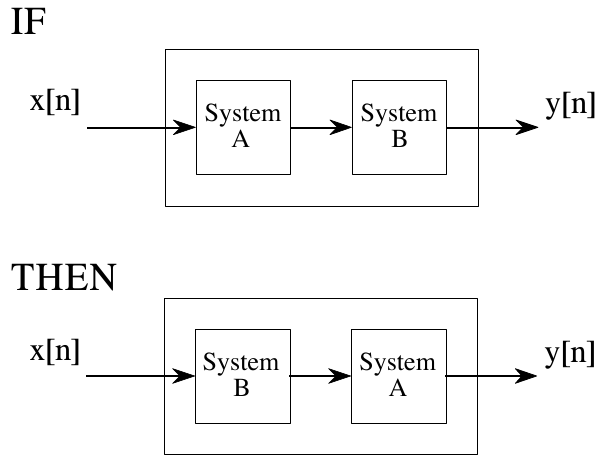
\includegraphics[width=0.508\linewidth,height=0.8\textheight,keepaspectratio]{assets/ch05/fig5-07.png}
\caption*{\textbf{图 5-7　线性系统的可交换性。}
两个或更多线性系统级联时，系统的顺序不影响整个组合的特性。 （IF =
如果，THEN = 那么，System A / System B = 系统 A / 系统 B。）}
\end{figure}

图 5-8
展示了线性系统理论的下一步：多输入和多输出。一个具有多个输入和/或多个输出的系统，如果由线性子系统和信号相加组成，它就是线性的。复杂程度无关紧要，只要系统内部不允许有任何非线性的东西。

为了理解线性对于多输入和/或多输出系统意味着什么，考虑下面这个思想实验。先在一个输入端加上一个信号，同时把其他输入端保持为零。这会使多个输出端以某种信号模式作出响应。接着，在另一个输入端加上另一个信号，重复这个过程。和前面一样，其他所有输入端都保持为零。第二个输入信号会使多个输出端出现另一种信号模式。最后，把两个信号同时加到各自的输入端。这时输出端出现的信号，就是两个输入信号分别单独施加时所产生的输出信号的叠加（和）。

\begin{figure}[htbp]
\centering
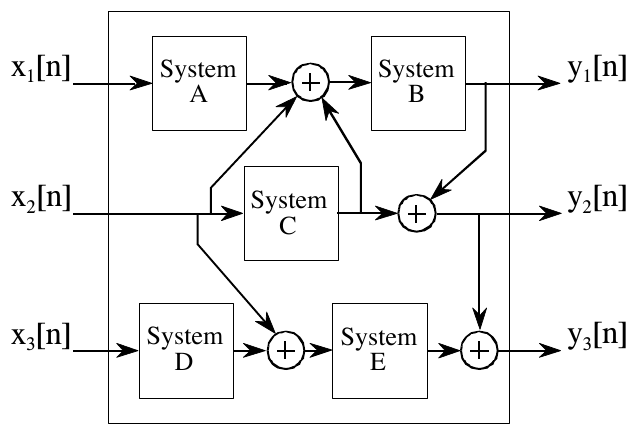
\includegraphics[width=0.533\linewidth,height=0.8\textheight,keepaspectratio]{assets/ch05/fig5-08.png}
\caption*{\textbf{图
5-8　任何具有多个输入和/或多个输出的系统，只要由线性系统和信号相加组成，就是线性的。}
（System A～E = 系统 A～E。）}
\end{figure}

线性系统中乘法的使用常常被误解。这是因为乘法可能是线性的，也可能是非线性的，取决于信号乘的是什么。图
5-9
说明了这两种情况。把输入信号乘以一个常数的系统是线性的。这个系统是放大器还是衰减器，取决于常数大于
1 还是小于
1。相反，把一个信号乘以另一个信号是非线性的。设想一个正弦波乘以另一个不同频率的正弦波，得到的波形显然不是正弦波。

另一个常被误解的情况，与电子电路中附加的寄生信号有关，比如直流偏移和热噪声。加入这些外来信号是线性的还是非线性的？答案取决于把这些污染信号看作从哪里来。如果把它们看作来自系统内部，这个过程就是非线性的，因为正弦输入产生的不是纯正弦输出。反过来，也可以把外来信号看作从多输入系统的一个单独输入端从外部进入系统。这样过程就是线性的，因为系统内部只需要做信号相加。

\begin{figure}[htbp]
\centering
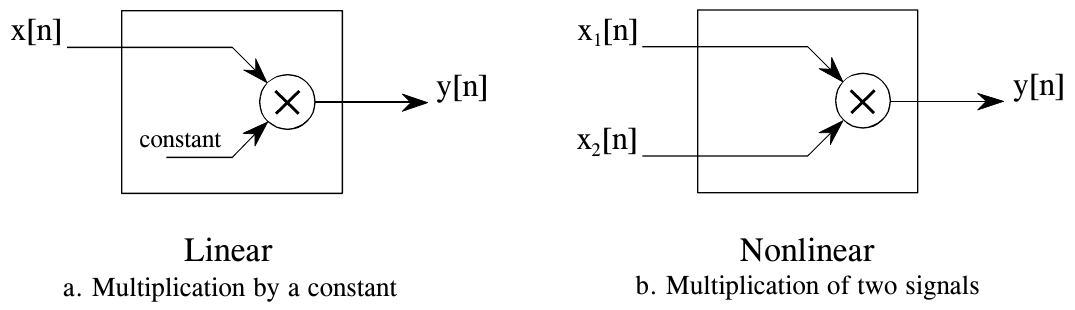
\includegraphics[width=0.896\linewidth,height=0.8\textheight,keepaspectratio]{assets/ch05/fig5-09.png}
\caption*{\textbf{图 5-9　乘法的线性。}
把信号乘以常数是线性运算。相反，两个信号相乘是非线性的。 （a.
乘以常数(Multiplication by a constant)，Linear = 线性；b.
两个信号相乘(Multiplication of two signals)，Nonlinear =
非线性。constant = 常数。）}
\end{figure}

\section{叠加：DSP 的基石}

处理线性系统时，信号唯一的组合方式是先缩放（把信号乘以常数）再相加。例如，一个信号不能乘以另一个信号。图
5-10 展示了一个例子：三个信号 \(x_0[n]\)、\(x_1[n]\) 和 \(x_2[n]\)
相加，形成第四个信号
x{[}n{]}。这种通过缩放和相加组合信号的过程叫合成(synthesis)。

分解(decomposition)是合成的逆运算：把一个信号拆成两个或更多个相加的分量。这比合成复杂，因为任何给定的信号都有无穷多种可能的分解。例如，15
和 25 两个数只能合成（相加）为 40。相比之下，40 可以分解为 1 + 39，或 2
+ 38，或 −30.5 + 60 + 10.5，等等。

\begin{figure}[htbp]
\centering
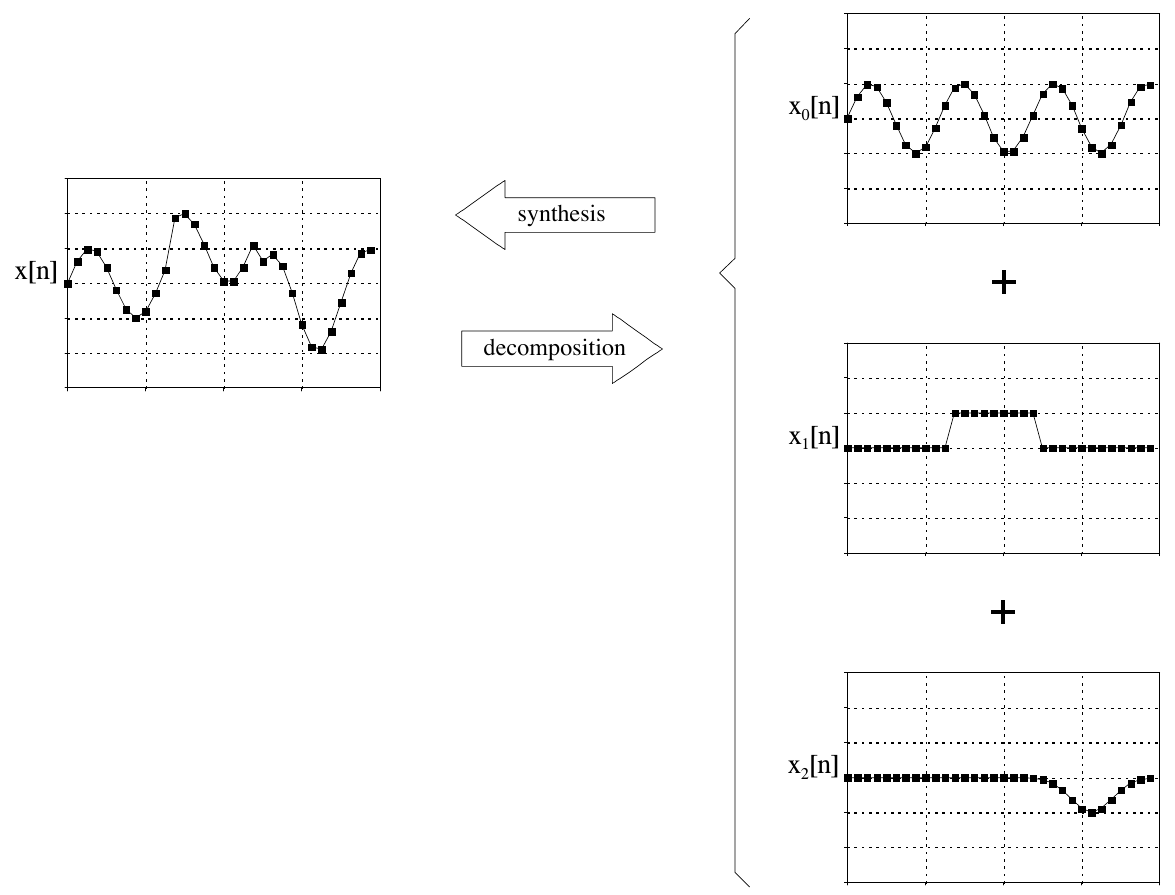
\includegraphics[width=0.979\linewidth,height=0.8\textheight,keepaspectratio]{assets/ch05/fig5-10.png}
\caption*{\textbf{图 5-10　信号的合成与分解示意。}
合成是把两个或更多信号相加，形成另一个信号。分解是相反的过程，把一个信号拆成两个或更多个相加的分量信号。
（synthesis = 合成，decomposition = 分解。）}
\end{figure}

现在我们来到了 DSP
的核心：叠加，理解怎样分析信号和系统的总体策略。考虑一个叫 x{[}n{]}
的输入信号通过一个线性系统，得到输出信号 y{[}n{]}。如图 5-11
所示，输入信号可以分解成一组更简单的信号：\(x_0[n]\)、\(x_1[n]\)、\(x_2[n]\)
等。我们把它们叫做输入信号分量。接着，让每个输入信号分量单独通过系统，得到一组输出信号分量：\(y_0[n]\)、\(y_1[n]\)、\(y_2[n]\)
等。然后把这些输出信号分量合成为输出信号 y{[}n{]}。

\begin{figure}[htbp]
\centering
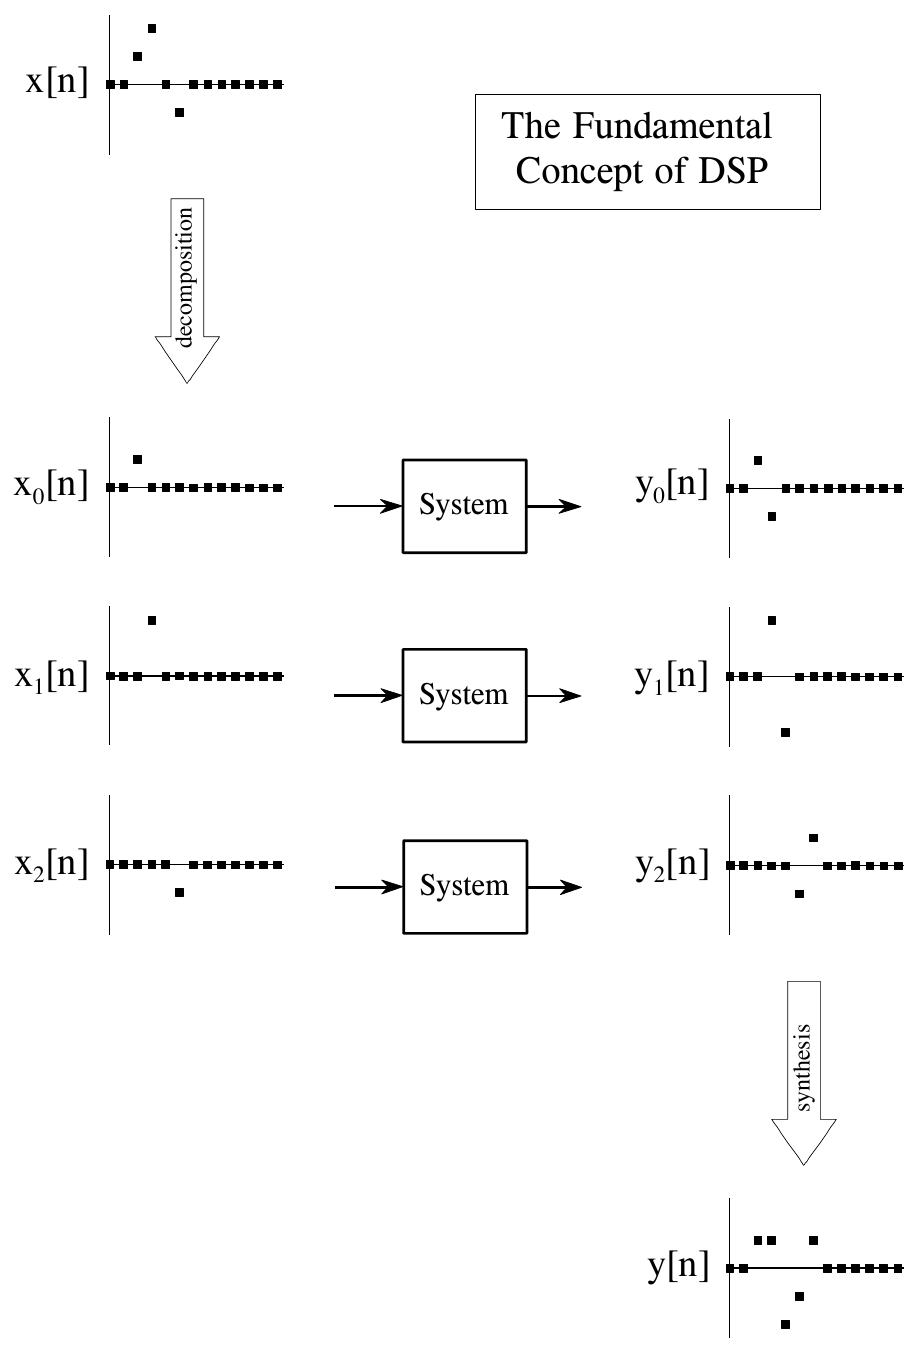
\includegraphics[width=0.762\linewidth,height=0.8\textheight,keepaspectratio]{assets/ch05/fig5-11.png}
\caption*{\textbf{图 5-11　DSP 的基本概念。} 任何信号，比如
x{[}n{]}，都可以分解成一组相加的分量，这里是信号 \(x_0[n]\)、\(x_1[n]\)
和 \(x_2[n]\)。让这些分量通过线性系统，产生信号 \(y_0[n]\)、\(y_1[n]\)
和 \(y_2[n]\)。把这些输出信号合成（相加），就得到 y{[}n{]}，它和
x{[}n{]} 直接通过系统所产生的信号相同。 （The Fundamental Concept of DSP
= DSP 的基本概念，decomposition = 分解，System = 系统，synthesis =
合成。原书图注把分量写成
\(x_1\)～\(x_3\)、\(y_1\)～\(y_3\)，与图中的下标 0～2
不一致，这里按图改正。）}
\end{figure}

重要的是：用这种方法得到的输出信号，和让输入信号直接通过系统所产生的输出信号完全相同。这是一个非常强大的思想。我们不必去弄懂复杂的信号会被系统怎样改变，只需要知道简单的信号会被怎样改变。用信号处理的行话说，输入和输出信号都被看作更简单波形的叠加（和）。这是几乎所有信号处理技术的基础。

举一个用叠加的简单例子：心算 2041 乘以
4。你是怎么算的？你可能想象脑海中漂浮着 2041
根火柴，把这幅画面变成四份，然后开始数。更可能的是，你用叠加简化了问题：2041
可以分解为 2000 + 40 + 1，把每个分量乘以 4 再合成，就得到最终答案，即
8000 + 160 + 4 = 8164。

\section{常见的分解方式}

记住，这个方法的目标是用几个简单的问题取代一个复杂的问题。如果分解没有在某种程度上简化情况，那就什么也没得到。信号处理中分解信号的主要方式有两种：冲激分解(impulse
decomposition)和傅里叶分解(Fourier
decomposition)。后面几章会详细介绍。此外，偶尔也会用到几种次要的分解。下面简要介绍两种主要的分解，以及三种次要的分解。

\subsection{冲激分解}

如图 5-12 所示，冲激分解把一个 N 个采样的信号拆成 N
个分量信号，每个分量信号也有 N
个采样。每个分量信号包含原始信号中的一个点，其余的值都为零。一串零中只有一个非零点，这叫冲激(impulse)。冲激分解很重要，因为它让我们可以一次考察信号的一个采样。同样，系统也用它对冲激的响应来刻画。只要知道系统怎样响应一个冲激，就能算出系统对任何给定输入的输出。这种方法叫卷积，是接下来两章的主题。

\subsection{阶跃分解}

图 5-13 所示的阶跃分解(step decomposition)，也是把一个 N
个采样的信号拆成 N 个分量信号，每个由 N
个采样组成。每个分量信号是一个阶跃(step)，即前面的采样值为零，后面的采样是某个常数值。考虑把一个
N 点信号 x{[}n{]} 分解成分量
\(x_0[n], x_1[n], x_2[n], \ldots, x_{N-1}[n]\)。第 k 个分量信号
\(x_k[n]\) 在第 0 到 k−1 点为零，其余各点的值为
\(x[k] - x[k-1]\)。例如，第 5 个分量信号 \(x_5[n]\) 在第 0 到 4
点为零，其余采样的值为 \(x[5] - x[4]\)（原始信号第 4 和第 5
个采样之差）。作为特例，\(x_0[n]\) 的所有采样都等于
x{[}0{]}。正如冲激分解一次看信号的一个点，阶跃分解用相邻采样之间的差来刻画信号。同样，系统也用它对输入信号变化的响应来刻画。

\begin{figure}[htbp]
\centering
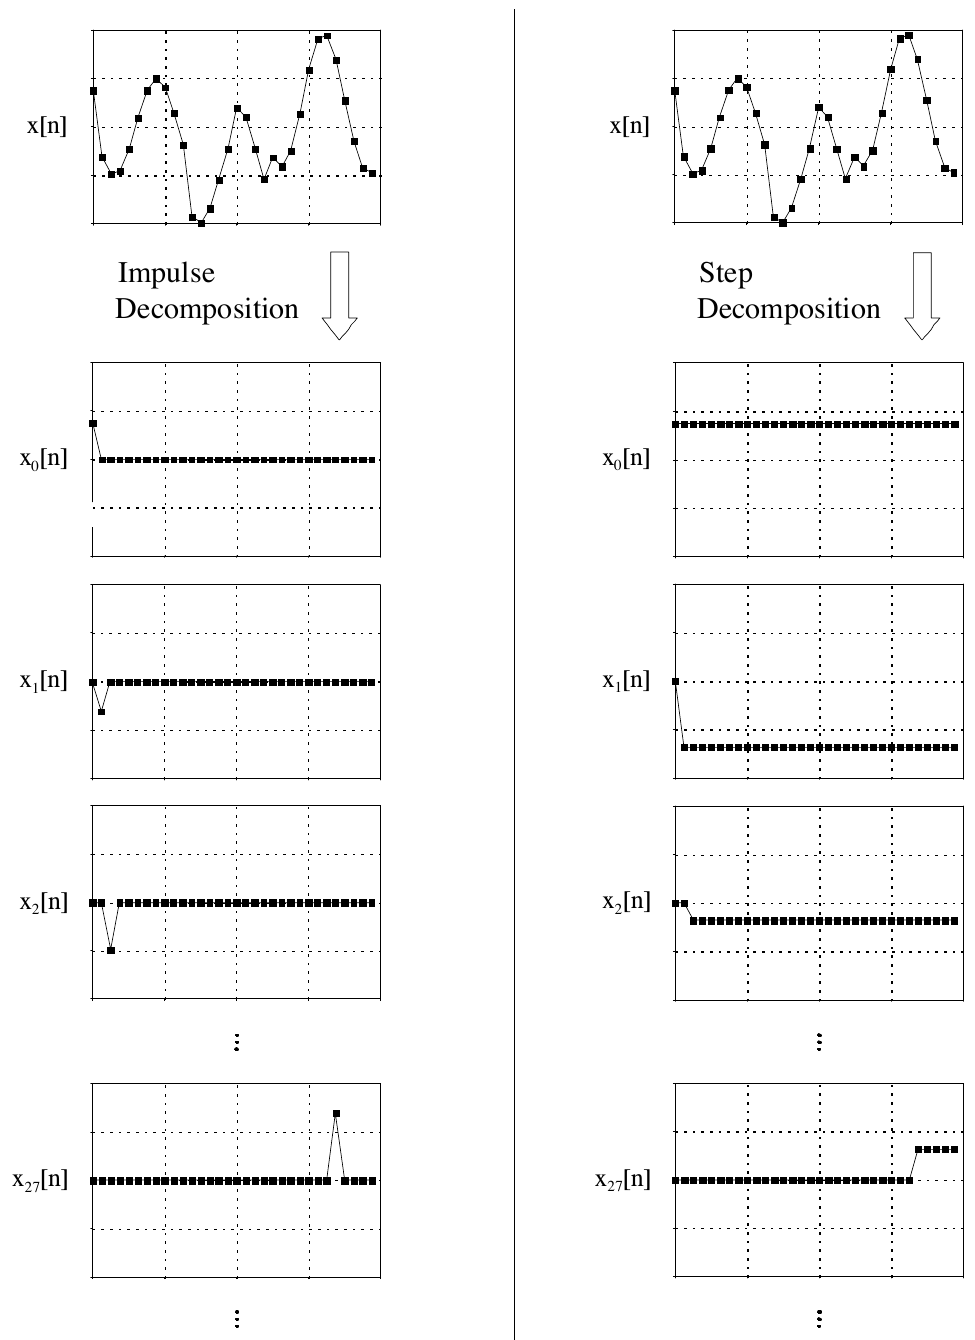
\includegraphics[width=0.812\linewidth,height=0.8\textheight,keepaspectratio]{assets/ch05/fig5-12-13.png}
\caption*{\textbf{图 5-12（左栏）　冲激分解的例子。} 一个 N 点信号被拆成 N
个分量，每个分量只有一个非零点。}
\end{figure}

\textbf{图 5-13（右栏）　阶跃分解的例子。} 一个 N 点信号被拆成 N
个信号，每个都是一个阶跃函数。 （Impulse Decomposition = 冲激分解，Step
Decomposition = 阶跃分解。两栏都只画出了 \(x_0\)、\(x_1\)、\(x_2\) 和
\(x_{27}\) 几个分量作示意。）

\subsection{偶/奇分解}

图 5-14 所示的偶/奇分解(even/odd
decomposition)，把一个信号拆成两个分量信号，一个具有偶对称性(even
symmetry)，另一个具有奇对称性(odd symmetry)。如果一个 N 点信号以第 N/2
点为中心左右镜像对称，就称它具有偶对称性。也就是说，采样 x{[}N/2+1{]}
必须等于 x{[}N/2−1{]}，x{[}N/2+2{]} 必须等于
x{[}N/2−2{]}，依此类推。类似地，如果对应点的幅值相等而符号相反，就是奇对称性，比如
x{[}N/2+1{]} = −x{[}N/2−1{]}，x{[}N/2+2{]} =
−x{[}N/2−2{]}，等等。这些定义假定信号由偶数个采样组成，索引从 0 到
N−1。分解按下面的关系计算：

\textbf{公式 5-1　偶/奇分解的公式。} 这两个公式把信号 x{[}n{]} 分成偶部
\(x_E[n]\) 和奇部
\(x_O[n]\)。由于这种分解基于循环对称性，偶信号和奇信号的第 0
个采样这样计算：\(x_E[0] = x[0]\)，\(x_O[0] = 0\)。所有信号都长 N
个采样，索引从 0 到 N−1。

\[
x_E[n] = \frac{x[n] + x[N-n]}{2}, \qquad x_O[n] = \frac{x[n] - x[N-n]}{2}
\]

这对左右对称的定义可能显得很奇怪，因为信号真正的中心是 N/2 −
½（在两个采样之间），而不是 N/2。同样，这种偏离中心的对称意味着第 0
个采样需要特殊处理。这是怎么回事？

这种分解是 DSP 中一个叫循环对称性(circular
symmetry)的重要概念的一部分。它把信号的末尾看作和信号的开头连在一起。正如
x{[}4{]} 挨着 x{[}5{]}，x{[}N−1{]} 也挨着
x{[}0{]}。想象一条咬住自己尾巴的蛇。用这种循环的方式看偶信号和奇信号时，实际上有两条对称轴，一条在
x{[}N/2{]}，另一条在 x{[}0{]}。例如，在偶信号中，绕 x{[}0{]}
的对称意味着 x{[}1{]} 等于 x{[}N−1{]}，x{[}2{]} 等于
x{[}N−2{]}，依此类推。在奇信号中，第 0 点和第 N/2
点的值总是零。在偶信号中，第 0 点和第 N/2 点等于原始信号中的对应点。

为什么要把信号的最后一个采样看作挨着第一个采样？常规的数据采集中没有任何东西支持这种循环的观念。事实上，第一个和最后一个采样之间的共同点，一般比序列中任何其他两点都少。这是常识！这个谜题缺失的一块，是一种叫傅里叶分析(Fourier
analysis)的 DSP
技术。傅里叶分析的数学本质上就把信号看作循环的，尽管就数据的来源而言，这通常没有物理意义。我们会在第
10 章更详细地讨论这一点。现在需要理解的重点是：公式 5-1
给出的是一个有效的分解，原因很简单：偶部和奇部相加就能重建原始信号。

\subsection{交错分解}

如图 5-15 所示，交错分解(interlaced
decomposition)把信号拆成两个分量信号：偶数采样信号和奇数采样信号（不要和偶对称、奇对称信号混淆）。求偶数采样信号：从原始信号出发，把所有奇数号采样设为零。求奇数采样信号：从原始信号出发，把所有偶数号采样设为零。就这么简单。

\begin{figure}[htbp]
\centering
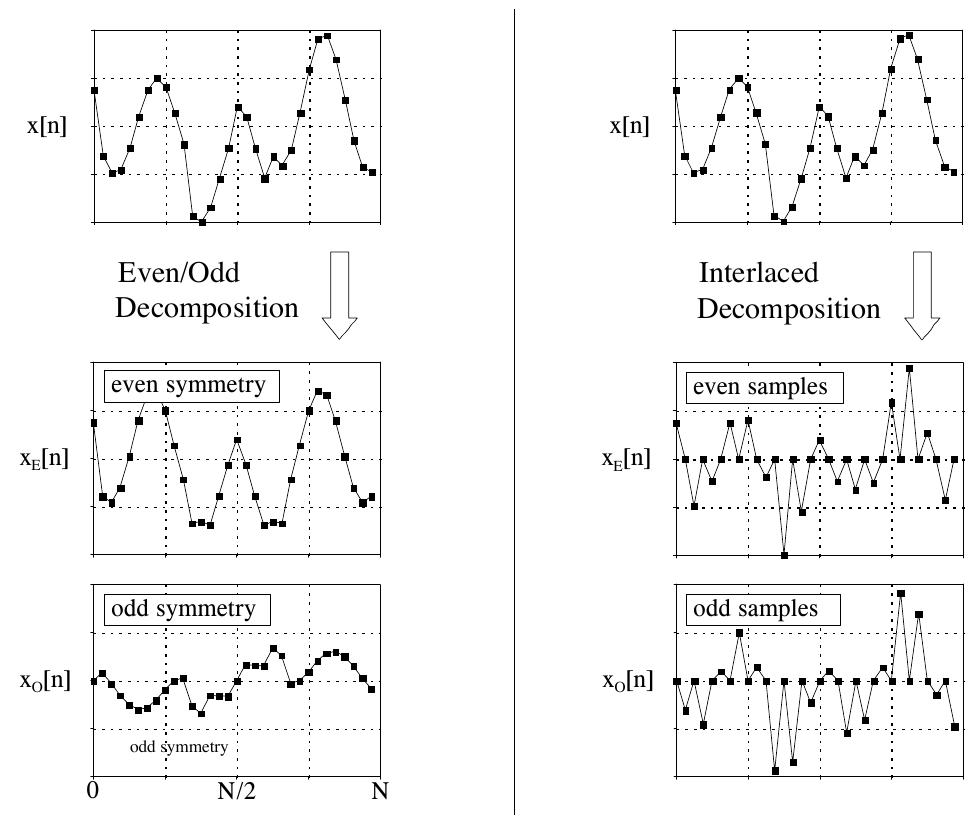
\includegraphics[width=0.812\linewidth,height=0.8\textheight,keepaspectratio]{assets/ch05/fig5-14-15.png}
\caption*{\textbf{图 5-14（左栏）　偶/奇分解的例子。} 一个 N 点信号被拆成两个 N
点信号，一个具有偶对称性，另一个具有奇对称性。}
\end{figure}

\textbf{图 5-15（右栏）　交错分解的例子。} 一个 N 点信号被拆成两个 N
点信号，一个把奇数号采样设为零，另一个把偶数号采样设为零。 （Even/Odd
Decomposition = 偶/奇分解，even symmetry = 偶对称，odd symmetry =
奇对称；Interlaced Decomposition = 交错分解，even samples =
偶数号采样，odd samples = 奇数号采样。）

乍一看，这种分解可能显得微不足道、毫无趣味。讽刺的是，交错分解正是 DSP
中一个极其重要的算法------快速傅里叶变换(FFT, Fast Fourier
Transform)------的基础。计算傅里叶分解的方法已经为人所知几百年了。可惜它慢得让人抓狂，在今天的计算机上常常要运行几分钟甚至几小时。FFT
是 20 世纪 60 年代发展起来的一族算法，用来缩短这个计算时间。它的策略是
DSP
的一个绝妙范例：反复使用交错变换，把信号化简成基本分量；计算各个分量的傅里叶分解；再把结果合成为最终答案。效果非常惊人，速度提高几百倍甚至几千倍是常事。

\subsection{傅里叶分解}

傅里叶分解非常数学化，一点也不直观。图 5-16
展示了这种技术的一个例子。任何 N 点信号都可以分解成 N+2
个信号，一半是正弦波，一半是余弦波。频率最低的余弦波（图中叫
\(x_{C0}[n]\)）在 N
个采样上完成零个完整周期，即它是一个直流信号。接下来的余弦分量
\(x_{C1}[n]\)、\(x_{C2}[n]\) 和 \(x_{C3}[n]\)，在 N 个采样上分别完成
1、2、3
个完整周期。其余的余弦波以及正弦分量都遵循这个模式。由于每个分量的频率是固定的，对不同的信号做分解时，唯一变化的是每个正弦波和余弦波的幅度。

\begin{figure}[htbp]
\centering
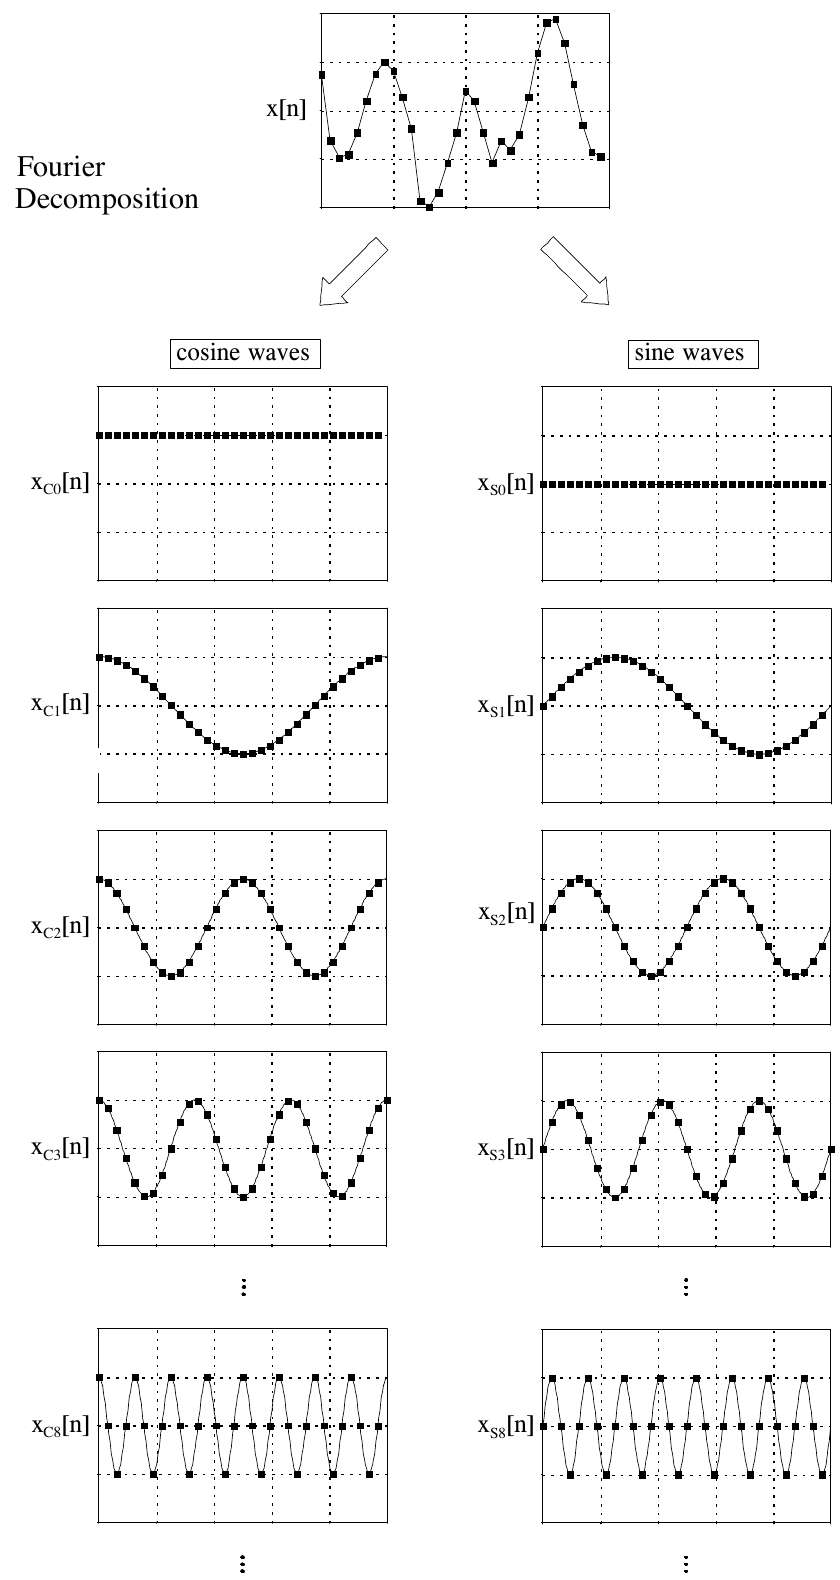
\includegraphics[width=0.700\linewidth,height=0.8\textheight,keepaspectratio]{assets/ch05/fig5-16.png}
\caption*{\textbf{图 5-16　傅里叶分解示意。} 一个 N 点信号被分解成 N+2
个信号，每个有 N
个点。其中一半是余弦波，一半是正弦波。这些正弦波的频率是固定的，只有幅度可以变化。
（Fourier Decomposition = 傅里叶分解，cosine waves = 余弦波，sine waves
= 正弦波。图中只画出了下标 0～3 和 8 的分量作示意。）}
\end{figure}

傅里叶分解之所以重要，有三个原因。第一，很多信号本来就是由叠加的正弦波产生的，音频信号就是一个很好的例子。傅里叶分解能直接分析这类信号中包含的信息。第二，线性系统对正弦波的响应方式很独特：正弦输入总是产生正弦输出。用这种方法，系统由它怎样改变通过它的正弦波的幅度和相位来刻画。由于输入信号可以分解成正弦波，只要知道系统对正弦波的反应，就能求出系统的输出。第三，傅里叶分解是一个广阔而强大的数学领域------傅里叶分析------的基础，也是更高级的拉普拉斯变换和
z 变换的基础。大多数最前沿的 DSP 算法都基于这些技术的某个方面。

为什么能把任意信号分解成正弦波和余弦波？对于一个具体的信号，这些正弦波的幅度怎样确定？用这种技术能设计出什么样的系统？这些问题要在后面的章节中回答。傅里叶分解的细节太复杂，没法在这个简短的概述中介绍。现在需要理解的重要思想是：把所有正弦分量加在一起，就能精确地重建原始信号。第
8 章会讲得更多。

\section{线性之外的替代方案}

要体会线性系统的重要性，想想看：分析非线性系统只有一种主要策略，那就是让非线性系统近似成线性系统。常用的做法有三种：

\textbf{第一，忽略非线性。}
如果非线性足够小，系统就可以近似为线性的。最初这个假设带来的误差，就当作噪声容忍，或者干脆忽略。

\textbf{第二，让信号保持很小。}
许多非线性系统在信号幅度很小时看起来是线性的。例如，晶体管在整个工作范围内非常非线性，但只要信号保持在几毫伏以下，就能提供准确的线性放大。运算放大器把这个思路发挥到了极致：利用非常高的开环增益加上负反馈，运放的输入信号（即反相输入端与同相输入端之间的差）只保持在几微伏。这微乎其微的输入信号，让一个原本非线性得可怕的电路表现出优异的线性。

\textbf{第三，施加一个线性化变换。}
例如，考虑两个信号相乘得到第三个信号：\(a[n] = b[n] \times c[n]\)。对信号取对数，就把乘法这个非线性过程变成了加法这个线性过程：\(\log(a[n]) = \log(b[n]) + \log(c[n])\)。这种方法有个好听的名字，叫同态信号处理(homomorphic
signal
processing)。例如，一幅视觉图像可以建模为场景的反射率（一个二维信号）乘以环境光照（另一个二维信号）。同态技术能让光照信号变得更均匀，从而改善图像。

在接下来的几章里，我们考察信号处理的两大主要技术：卷积和傅里叶分析。两者都基于本章介绍的策略：(1)
把信号分解成简单的相加分量；(2) 以某种有用的方式处理这些分量；(3)
把这些分量合成为最终结果。这就是 DSP。

% !TEX root = ../main.tex
% 本文件由 build-tex.sh 从 06-DSP指南-第6章中译.md 生成，改内容请改 md 后重新生成

\chapter{卷积}\label{ch-06}

卷积(convolution)是把两个信号组合成第三个信号的一种数学方法。它是数字信号处理中最重要的一项技术。利用冲激分解的策略，系统用一个叫冲激响应(impulse
response)的信号来描述。卷积之所以重要，是因为它把我们关心的三个信号联系在一起：输入信号、输出信号和冲激响应。本章从两个不同的角度介绍卷积，分别叫输入端算法(input
side algorithm)和输出端算法(output side algorithm)。卷积为 DSP
提供了数学框架，本书没有比它更重要的内容了。

\section{冲激函数与冲激响应}

上一章讲了怎样把一个信号分解成一组叫冲激(impulse)的分量。冲激是除一个非零点外全为零的信号。实际上，冲激分解提供了一种一次分析信号一个采样的方法。上一章还介绍了
DSP
的基本概念：把输入信号分解成简单的相加分量，让每个分量通过线性系统，再把得到的输出分量合成（相加）。这种分而治之的做法得到的信号，和把原始信号直接通过系统得到的信号完全相同。可能的分解虽然很多，但构成信号处理骨架的只有两种：冲激分解和傅里叶分解。使用冲激分解时，这个过程可以用一种叫卷积的数学运算来描述。本章（以及后面大多数章节）只讨论离散信号。卷积也适用于连续信号，但数学更复杂。第
13 章会讲连续信号怎样处理。

图 6-1 定义了 DSP 中两个重要的术语。第一个是冲激函数(delta
function)，用希腊字母 delta 表示，记作
δ{[}n{]}。冲激函数是归一化的冲激，即第 0 个采样的值为
1，其余所有采样的值都为 0。因此，冲激函数也常被称为单位冲激(unit
impulse)。

图 6-1
定义的第二个术语是冲激响应。顾名思义，冲激响应就是输入为冲激函数（单位冲激）时系统输出的信号。两个系统只要有任何不同，它们的冲激响应就不同。正如输入和输出信号常被叫做
x{[}n{]} 和 y{[}n{]}，冲激响应通常用符号 h{[}n{]}
表示。当然，如果有更具描述性的名字也可以换，比如可以用 f{[}n{]}
来表示一个滤波器(filter)的冲激响应。

\begin{figure}[htbp]
\centering
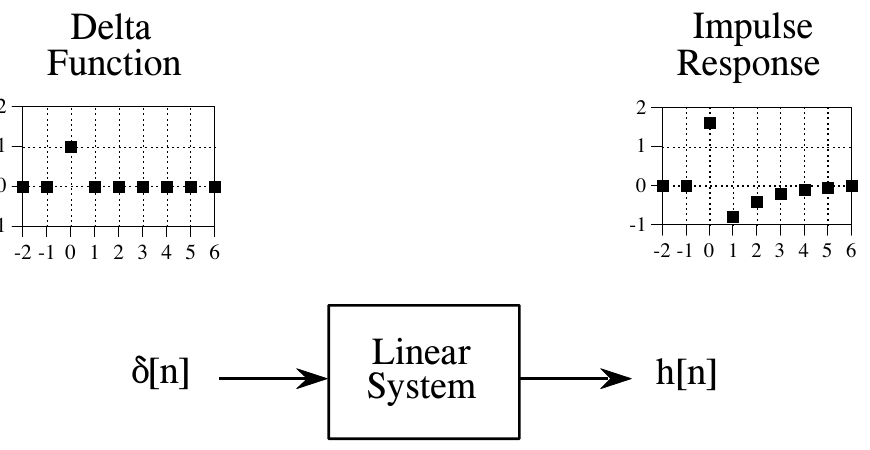
\includegraphics[width=0.725\linewidth,height=0.8\textheight,keepaspectratio]{assets/ch06/fig6-01.png}
\caption*{\textbf{图 6-1　冲激函数和冲激响应的定义。} 冲激函数是归一化的冲激：除第
0 个采样的值为 1 外，所有采样的值都为 0。用希腊字母 delta，即
δ{[}n{]}，表示冲激函数。线性系统的冲激响应通常记作
h{[}n{]}，是输入为冲激函数时系统的输出。 （Delta Function =
冲激函数，Impulse Response = 冲激响应，Linear System = 线性系统；图中
δ{[}n{]} 在原书 PDF 抽取时显示为 *{[}n{]}。）}
\end{figure}

任何冲激都可以表示为一个经过平移和缩放的冲激函数。考虑一个信号
a{[}n{]}，除第 8 个采样的值为 −3 外全为零。这和把冲激函数向右平移 8
个采样、再乘以 −3
是一回事。写成公式：\(a[n] = -3\,\delta[n-8]\)。一定要弄懂这种记法，几乎所有
DSP 公式都会用到它。

如果系统的输入是一个冲激，比如
\(-3\,\delta[n-8]\)，系统的输出是什么？这里就要用到齐次性和平移不变性：对输入做缩放和平移，输出也会做同样的缩放和平移。如果
δ{[}n{]} 产生 h{[}n{]}，那么 \(-3\,\delta[n-8]\) 就产生
\(-3\,h[n-8]\)。用文字说，输出是冲激响应的一个版本，它的平移量和缩放量与输入端的冲激函数相同。只要知道系统的冲激响应，你立刻就知道它对任何冲激会作出什么反应。

\section{卷积}

我们来总结一下这种理解系统怎样把输入信号变成输出信号的方式。第一，输入信号可以分解成一组冲激，每个冲激都可以看作一个经过缩放和平移的冲激函数。第二，每个冲激产生的输出，是冲激响应的一个经过缩放和平移的版本。第三，把这些经过缩放和平移的冲激响应加起来，就得到总的输出信号。换句话说，只要知道系统的冲激响应，就能算出任何可能的输入信号对应的输出。这意味着我们知道了关于这个系统的一切。关于线性系统的特性，再没有别的东西可学了。（不过在后面的章节中我们会看到，这些信息可以用不同的形式表示。）

在某些应用中，冲激响应有别的名字。如果所考虑的系统是滤波器，冲激响应就叫滤波器核(filter
kernel)、卷积核(convolution
kernel)，或者简称核(kernel)。在图像处理中，冲激响应叫点扩散函数(point
spread
function)。这些术语的用法虽然略有不同，但意思都一样：输入为冲激函数时系统产生的信号。

卷积是一种正式的数学运算，就像乘法、加法和积分一样。加法取两个数产生第三个数，而卷积取两个信号产生第三个信号。卷积在许多领域的数学中都有应用，比如概率和统计。在线性系统中，卷积用来描述我们关心的三个信号之间的关系：输入信号、冲激响应和输出信号。

图 6-2 展示了在线性系统中使用卷积时的记法。输入信号 x{[}n{]}
进入一个冲激响应为 h{[}n{]} 的线性系统，得到输出信号
y{[}n{]}。写成公式：\(x[n] * h[n] = y[n]\)。用文字说，输入信号与冲激响应的卷积等于输出信号。正如加法用加号
+ 表示、乘法用叉号 × 表示，卷积用星号 \dspsym{∗}
表示。遗憾的是，大多数编程语言也用星号表示乘法。程序里的星号表示乘法，而公式里的星号表示卷积。

\begin{figure}[htbp]
\centering
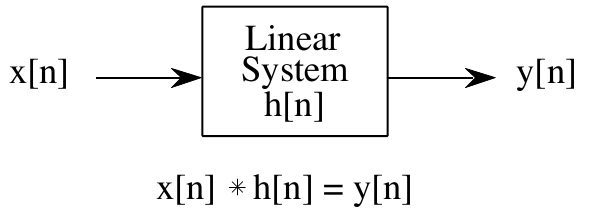
\includegraphics[width=0.492\linewidth,height=0.8\textheight,keepaspectratio]{assets/ch06/fig6-02.png}
\caption*{\textbf{图 6-2　DSP 中怎样使用卷积。}
线性系统的输出信号等于输入信号与系统冲激响应的卷积。写公式时，卷积用星号表示。}
\end{figure}

图 6-3
展示了用卷积做低通滤波和高通滤波。示例输入信号是两个分量之和：三个周期的正弦波（代表高频），加上一个缓慢上升的斜坡（由低频组成）。在
(a)
中，低通滤波器的冲激响应是一条平滑的拱形，结果只有缓慢变化的斜坡波形通过到输出。类似地，(b)
中的高通滤波器只让变化更快的正弦波通过。

\begin{figure}[htbp]
\centering
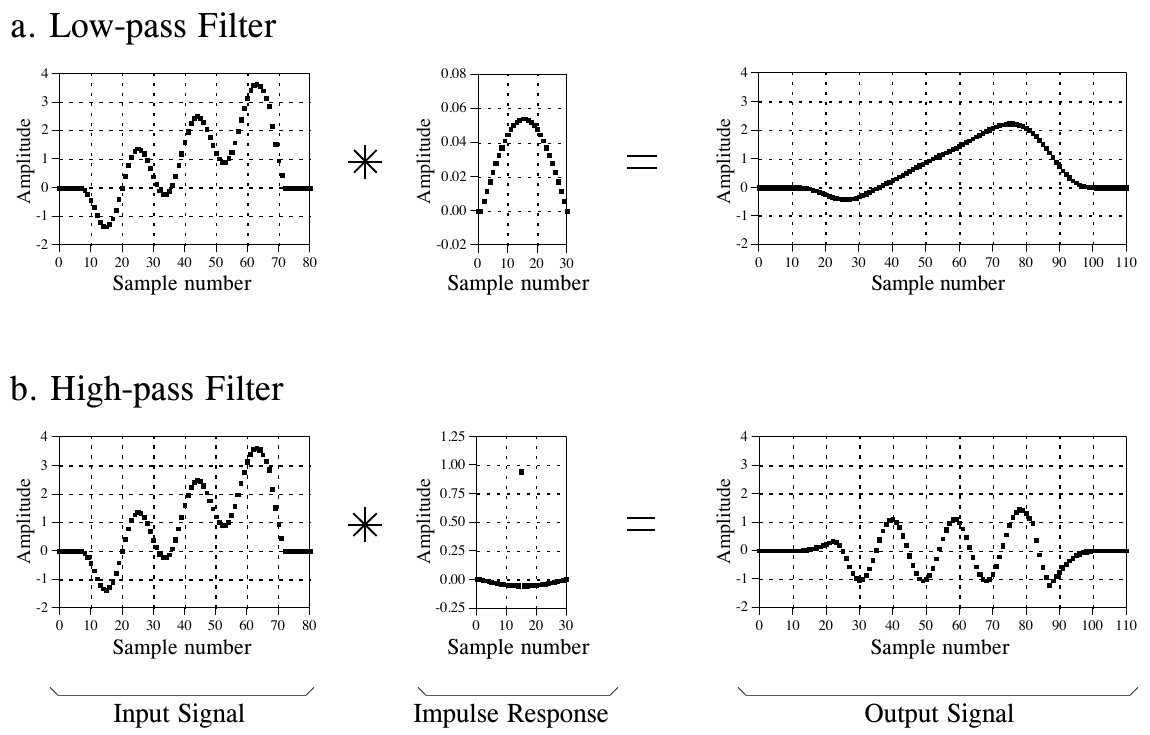
\includegraphics[width=0.958\linewidth,height=0.8\textheight,keepaspectratio]{assets/ch06/fig6-03.png}
\caption*{\textbf{图 6-3　用卷积做低通和高通滤波的例子。}
本例中，输入信号是几个周期的正弦波加上一个缓慢上升的斜坡。选取合适的冲激响应，就能把这两个分量分开。
（a. 低通滤波器(Low-pass Filter)；b. 高通滤波器(High-pass
Filter)。三栏依次为 Input Signal = 输入信号、Impulse Response =
冲激响应、Output Signal = 输出信号。Amplitude = 幅度，Sample number =
采样序号。）}
\end{figure}

图 6-4 给出了另外两个用卷积处理信号的例子。(a) 中的反相衰减器(inverting
attenuator)把信号上下翻转，并减小其幅度。(b) 中的离散导数(discrete
derivative，也叫一阶差分(first
difference))产生的输出信号与输入信号的斜率有关。

\begin{figure}[htbp]
\centering
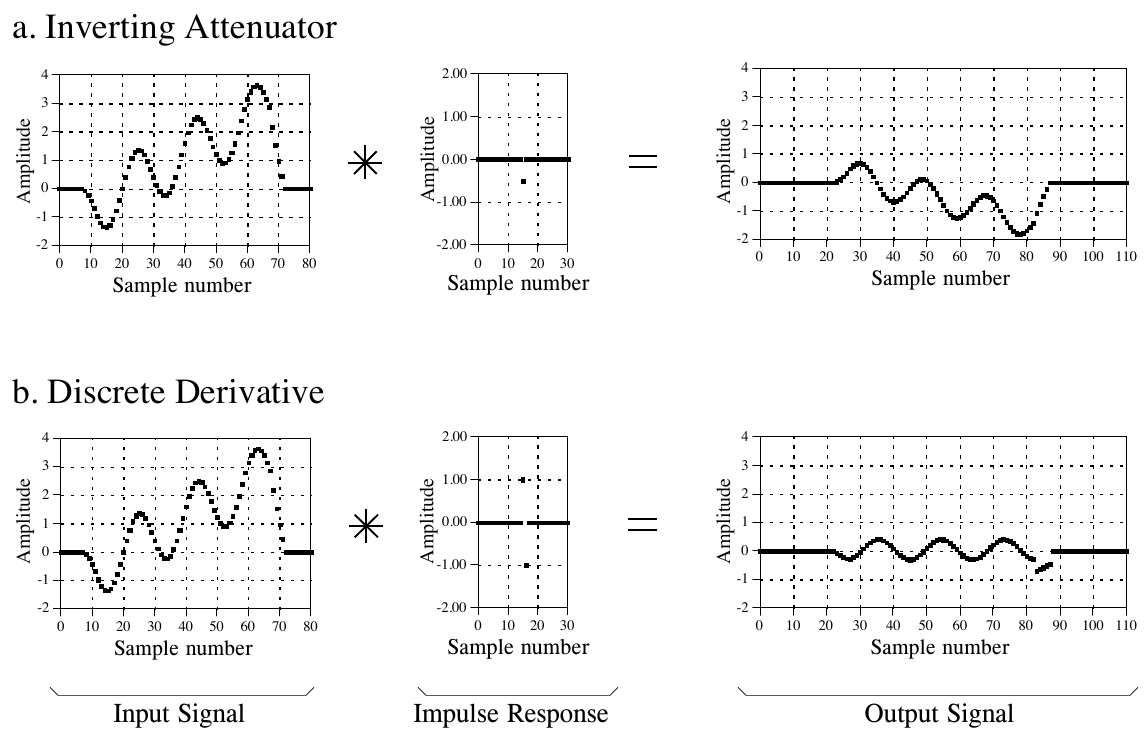
\includegraphics[width=0.954\linewidth,height=0.8\textheight,keepaspectratio]{assets/ch06/fig6-04.png}
\caption*{\textbf{图 6-4　用卷积处理信号的例子。}
许多信号处理任务用的冲激响应都非常简单。如这些例子所示，只用几个非零点就能产生显著的变化。
（a. 反相衰减器(Inverting Attenuator)；b. 离散导数(Discrete
Derivative)。三栏依次为输入信号、冲激响应、输出信号。）}
\end{figure}

注意图 6-3 和 6-4 中各信号的长度。输入信号长 81 个采样，每个冲激响应由
31 个采样组成。在大多数 DSP
应用中，输入信号长几百、几千甚至几百万个采样。冲激响应通常短得多，比如几个点到几百个点。卷积背后的数学并不限制这些信号有多长，但它确实规定了输出信号的长度：输出信号的长度等于输入信号的长度加上冲激响应的长度再减一。对于图
6-3 和 6-4 中的信号，每个输出信号长 81 + 31 − 1 = 111
个采样。输入信号从第 0 到第 80 个采样，冲激响应从第 0 到第 30
个采样，输出信号从第 0 到第 110 个采样。

现在来看卷积的详细数学。在数字信号处理中，卷积可以用两种不同的方式来理解。第一种从输入信号的角度看卷积：分析输入信号中的每个采样怎样影响输出信号中的许多点。第二种从输出信号的角度看卷积：考察输出信号中的每个采样怎样从输入信号的许多点接收信息。记住，这两个视角是对同一个数学运算的不同思考方式。第一个视角很重要，因为它提供了卷积与
DSP 有何关系的概念性理解。第二个视角描述了卷积的数学。这体现了你在 DSP
中会遇到的最难的任务之一：让你的概念性理解和用来交流这些想法的一堆数学对上号。

\section{输入端算法}

图 6-5 展示了一个简单的卷积问题：一个 9 点输入信号 x{[}n{]}
通过一个冲激响应为 4 点 h{[}n{]} 的系统，得到一个 9 + 4 − 1 = 12
点的输出信号 y{[}n{]}。用数学语言说，x{[}n{]} 与 h{[}n{]} 卷积得到
y{[}n{]}。卷积的第一个视角基于 DSP
的基本概念：分解输入，让各分量通过系统，再合成输出。在这个例子中，输入信号的九个采样中的每一个，都会给输出信号贡献一个经过缩放和平移的冲激响应。这九个信号如图
6-6 所示。把这九个信号相加，就得到输出信号 y{[}n{]}。

\begin{figure}[htbp]
\centering
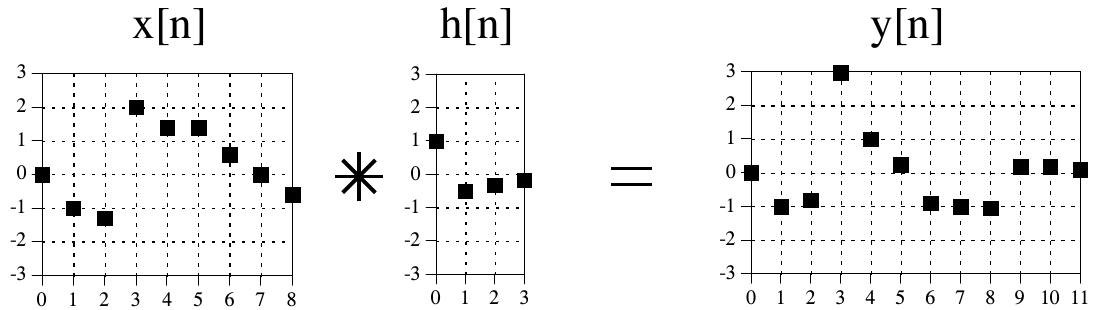
\includegraphics[width=0.912\linewidth,height=0.8\textheight,keepaspectratio]{assets/ch06/fig6-05.png}
\caption*{\textbf{图 6-5　卷积问题示例。}
一个九点的输入信号与一个四点的冲激响应卷积，得到一个十二点的输出信号。输入信号中的每个点都给输出信号贡献一个经过缩放和平移的冲激响应。这九个经过缩放和平移的冲激响应如图
6-6 所示。}
\end{figure}

我们详细看看这九个信号中的几个。先从输入信号的第 4 个采样，即 x{[}4{]}
开始。这个采样位于索引 4，值为 1.4。分解信号时，它变成一个冲激，表示为
\(1.4\,\delta[n-4]\)。通过系统后，得到的输出分量是
\(1.4\,h[n-4]\)。这个信号就是图 6-6
九个信号中正中间那个方框。注意，这是冲激响应 h{[}n{]} 乘以
1.4、再向右平移四个采样的结果。第 0～3 和第 8～11
个采样处补了零作为占位符。为了更清楚，图 6-6
用方块表示来自平移和缩放后冲激响应的数据点，用菱形表示补上的零。

现在看采样 x{[}8{]}，即输入信号的最后一个点。这个采样位于索引 8，值为
−0.5。如图 6-6 右下角的图所示，x{[}8{]} 产生一个向右平移八个点并乘以
−0.5 的冲激响应。第 0～7 点补了零作为占位符。最后，看看 x{[}0{]} 和
x{[}7{]}
这两个点的作用。这两个采样的值都为零，因此产生的输出分量全为零。

\begin{figure}[htbp]
\centering
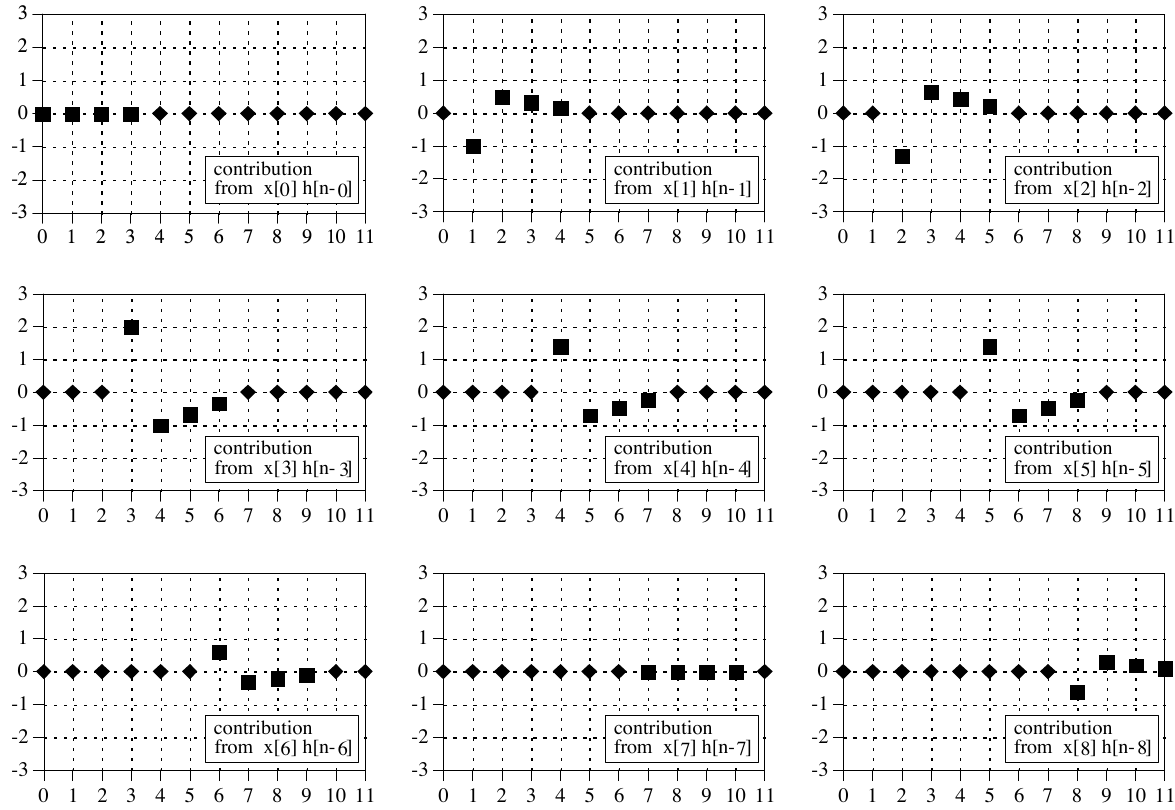
\includegraphics[width=0.979\linewidth,height=0.8\textheight,keepaspectratio]{assets/ch06/fig6-06.png}
\caption*{\textbf{图 6-6　图 6-5 卷积的输出信号分量。}
在这些信号中，来自缩放和平移后冲激响应的点用方块标记表示。其余的数据点用菱形表示，是作为占位符补上的零。
（contribution from x{[}k{]} h{[}n−k{]} = 由 x{[}k{]} 贡献的
h{[}n−k{]}，k = 0～8。）}
\end{figure}

在这个例子中，x{[}n{]} 是九点信号，h{[}n{]} 是四点信号。在下一个例子（图
6-7）中，我们把情况反过来：让 x{[}n{]} 是四点信号，h{[}n{]}
是九点信号。用的还是这两个波形，只是交换了一下。从输出信号分量可以看出，x{[}n{]}
的四个采样产生了九点冲激响应的四个经过平移和缩放的版本。和前面一样，前后补零作为占位符。

等一下！图 6-7 的输出信号和图 6-5
的输出信号完全相同。这不是错误，而是一个重要的性质：卷积满足交换律(commutative)，\(a[n] * b[n] = b[n] * a[n]\)。数学并不在乎哪个是输入信号、哪个是冲激响应，只在乎两个信号相互卷积。数学虽然允许这样做，但在系统理论中交换这两个信号没有物理意义。输入信号和冲激响应是完全不同的两样东西，交换它们说不通。交换律提供的是一个数学工具，用来变换公式以得到各种结果。

\begin{figure}[htbp]
\centering
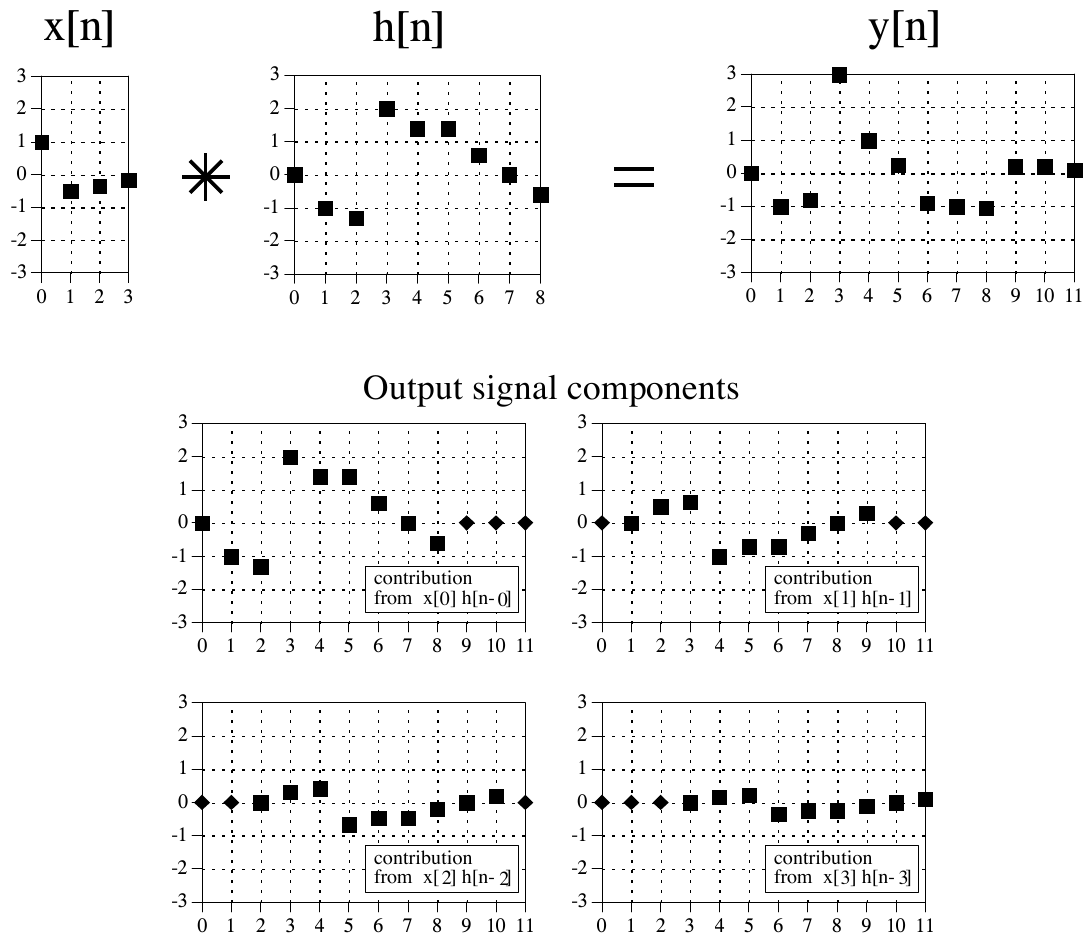
\includegraphics[width=0.908\linewidth,height=0.8\textheight,keepaspectratio]{assets/ch06/fig6-07.png}
\caption*{\textbf{图 6-7　卷积的第二个例子。} 输入信号和冲激响应的波形与图 6-5
的例子互换了。由于卷积满足交换律，两个例子的输出信号完全相同。 （Output
signal components = 输出信号分量。）}
\end{figure}

表 6-1
是一个用输入端算法计算卷积的程序。记住，本书的程序旨在以最简单的形式传达算法，哪怕牺牲良好的编程风格。例如，所有输入和输出都在虚构的子程序（第
160 和 280
行）中处理，也就是说，我们并不定义这些操作具体怎样进行。不要跳过这些程序，它们是内容的关键部分，你需要详细理解。

这个程序把存放在数组 X{[} {]} 中的 81 点输入信号，与存放在数组 H{[} {]}
中的 31 点冲激响应卷积，得到存放在数组 Y{[} {]} 中的 111
点输出信号。这和图 6-3、6-4
中的长度相同。注意这些数组名用的是大写字母。这违反了前面讲的命名约定，因为大写字母是留给频域信号的。可惜本书用的简单
BASIC 不允许小写变量名。还要注意，第 240
行用星号表示乘法。记住，程序里的星号表示乘法，公式里的星号表示卷积。文字（比如文档或程序注释）中的星号两者都可能。

第 160 行的虚构子程序把输入信号放进 X{[} {]}，把冲激响应放进 H{[}
{]}。第 180～200 行把 Y{[} {]} 的所有值设为零。这是必要的，因为 Y{[} {]}
被用作累加器，在计算输出分量的过程中把它们加起来。第 220～260
行是程序的核心。第 220 行的 FOR 语句控制一个循环，逐个遍历输入信号 X{[}
{]} 中的每个点。对输入信号中的每个采样，内层循环（第 230～250
行）计算冲激响应的一个经过缩放和平移的版本，并把它加到累积输出信号的数组
Y{[} {]}
中。这种嵌套循环结构（一个循环套在另一个循环里）是卷积程序的一个关键特征，要熟悉它。

\textbf{表 6-1}（注释已译成中文）

\begin{Shaded}
\begin{Highlighting}[]
\NormalTok{100 \textquotesingle{}CONVOLUTION USING THE INPUT SIDE ALGORITHM}
\NormalTok{110 \textquotesingle{}}
\NormalTok{120 DIM X[80]                   \textquotesingle{}输入信号，81 点}
\NormalTok{130 DIM H[30]                   \textquotesingle{}冲激响应，31 点}
\NormalTok{140 DIM Y[110]                  \textquotesingle{}输出信号，111 点}
\NormalTok{150 \textquotesingle{}}
\NormalTok{160 GOSUB XXXX                  \textquotesingle{}虚构的子程序，载入 X[ ] 和 H[ ]}
\NormalTok{170 \textquotesingle{}}
\NormalTok{180 FOR I\% = 0 TO 110           \textquotesingle{}把输出数组清零}
\NormalTok{190   Y(I\%) = 0}
\NormalTok{200 NEXT I\%}
\NormalTok{210 \textquotesingle{}}
\NormalTok{220 FOR I\% = 0 TO 80            \textquotesingle{}遍历 X[ ] 中的每个点}
\NormalTok{230   FOR J\% = 0 TO 30          \textquotesingle{}遍历 H[ ] 中的每个点}
\NormalTok{240     Y[I\%+J\%] = Y[I\%+J\%] + X[I\%]*H[J\%]}
\NormalTok{250   NEXT J\%}
\NormalTok{260 NEXT I\%                     \textquotesingle{}（记住，程序里的 * 是乘法！）}
\NormalTok{270 \textquotesingle{}}
\NormalTok{280 GOSUB XXXX                  \textquotesingle{}虚构的子程序，保存 Y[ ]}
\NormalTok{290 \textquotesingle{}}
\NormalTok{300 END}
\end{Highlighting}
\end{Shaded}

\textbf{C 实现}（完整可编译版本见
\texttt{c/table6-1\_convolve\_input\_side.c}，其中用图 6-3a
的设定生成了输入信号和低通冲激响应）：

\begin{Shaded}
\begin{Highlighting}[]
\PreprocessorTok{\#define NX }\DecValTok{81}\PreprocessorTok{                   }\CommentTok{/* 120 DIM X[80]：输入信号 81 点 */}
\PreprocessorTok{\#define NH }\DecValTok{31}\PreprocessorTok{                   }\CommentTok{/* 130 DIM H[30]：冲激响应 31 点 */}
\PreprocessorTok{\#define NY }\OperatorTok{(}\PreprocessorTok{NX }\OperatorTok{+}\PreprocessorTok{ NH }\OperatorTok{{-}}\PreprocessorTok{ }\DecValTok{1}\OperatorTok{)}\PreprocessorTok{        }\CommentTok{/* 140 DIM Y[110]：输出信号 111 点 */}

\CommentTok{/* 输入端算法：输入的每个点，都往输出里加一份缩放、平移后的冲激响应 */}
\DataTypeTok{static} \DataTypeTok{void}\NormalTok{ convolve\_input\_side}\OperatorTok{(}\DataTypeTok{const} \DataTypeTok{double} \OperatorTok{*}\NormalTok{x}\OperatorTok{,} \DataTypeTok{const} \DataTypeTok{double} \OperatorTok{*}\NormalTok{h}\OperatorTok{,} \DataTypeTok{double} \OperatorTok{*}\NormalTok{y}\OperatorTok{)}
\OperatorTok{\{}
    \ControlFlowTok{for} \OperatorTok{(}\DataTypeTok{int}\NormalTok{ i }\OperatorTok{=} \DecValTok{0}\OperatorTok{;}\NormalTok{ i }\OperatorTok{\textless{}}\NormalTok{ NY}\OperatorTok{;}\NormalTok{ i}\OperatorTok{++)}        \CommentTok{/* 180～200：输出数组清零，后面当累加器用 */}
\NormalTok{        y}\OperatorTok{[}\NormalTok{i}\OperatorTok{]} \OperatorTok{=} \FloatTok{0.0}\OperatorTok{;}

    \ControlFlowTok{for} \OperatorTok{(}\DataTypeTok{int}\NormalTok{ i }\OperatorTok{=} \DecValTok{0}\OperatorTok{;}\NormalTok{ i }\OperatorTok{\textless{}}\NormalTok{ NX}\OperatorTok{;}\NormalTok{ i}\OperatorTok{++)}        \CommentTok{/* 220：遍历输入的每个点 */}
        \ControlFlowTok{for} \OperatorTok{(}\DataTypeTok{int}\NormalTok{ j }\OperatorTok{=} \DecValTok{0}\OperatorTok{;}\NormalTok{ j }\OperatorTok{\textless{}}\NormalTok{ NH}\OperatorTok{;}\NormalTok{ j}\OperatorTok{++)}    \CommentTok{/* 230：遍历冲激响应的每个点 */}
\NormalTok{            y}\OperatorTok{[}\NormalTok{i }\OperatorTok{+}\NormalTok{ j}\OperatorTok{]} \OperatorTok{+=}\NormalTok{ x}\OperatorTok{[}\NormalTok{i}\OperatorTok{]} \OperatorTok{*}\NormalTok{ h}\OperatorTok{[}\NormalTok{j}\OperatorTok{];}    \CommentTok{/* 240：缩放（乘 x[i]）、平移（下标 +i）、累加 */}
\OperatorTok{\}}
\end{Highlighting}
\end{Shaded}

第 240 行的下标很容易把人绕晕！假设程序执行到一半，刚开始处理采样
X{[}40{]}，即 I\% =
40。内层循环遍历冲激响应的每个点，做三件事。第一，把冲激响应乘以这个输入采样的值来缩放。如果内层循环只做这一件事，第
240 行可以写成
\texttt{Y{[}J\%{]}\ =\ X{[}40{]}*H{[}J\%{]}}。第二，给输出信号所用的下标加上
40，把缩放后的冲激响应向右平移 40 个采样。这第二个动作会把第 240 行变成
\texttt{Y{[}40+J\%{]}\ =\ X{[}40{]}*H{[}J\%{]}}。第三，Y{[} {]}
必须累加（合成）输入信号中每个采样产生的所有信号。因此，新信息必须加到数组中已有的信息上。于是得到最终的命令：\texttt{Y{[}40+J\%{]}\ =\ Y{[}40+J\%{]}\ +\ X{[}40{]}*H{[}J\%{]}}。仔细研究一下，它非常绕，但非常重要。

\section{输出端算法}

卷积的第一个视角分析的是输入信号中的每个采样怎样影响输出信号中的许多采样。在第二个视角中，我们反过来：看输出信号中的单个采样，找出输入中对它有贡献的点。无论从数学还是实用的角度看，这都很重要。假设给定某个输入信号和冲激响应，要求两者的卷积。最直接的方法是写一个程序遍历输出信号，每次循环算出一个采样。同样，公式也写成这样的形式：y{[}n{]}
= 其他变量的某种组合。也就是说，输出信号的第 n
个采样等于输入信号和冲激响应中许多值的某种组合。这要求我们知道输出信号中的每个采样怎样独立于输出信号中所有其他采样计算出来。输出端算法提供的正是这个信息。

我们来看一个例子，看输出信号中的单个点怎样受输入中几个点的影响。我们用图
6-5 中的 y{[}6{]} 作例子。这个点等于图 6-6 中九个输出分量的第 6
个点之和。现在仔细看这九个输出分量，找出哪些能影响
y{[}6{]}，即这九个信号中哪些在第 6
个位置上有非零采样。有五个输出分量在第 6
个采样处只有补上的零（菱形标记），因此可以忽略。只有四个输出分量可能在第
6 个位置上有非零值。它们是由输入采样 x{[}3{]}、x{[}4{]}、x{[}5{]} 和
x{[}6{]} 产生的输出分量。把这些输出分量的第 6 个采样加起来，就确定了
y{[}6{]}：\(y[6] = x[3]h[3] + x[4]h[2] + x[5]h[1] + x[6]h[0]\)。也就是说，输入信号的四个采样与冲激响应的四个采样相乘，再把乘积相加。

图 6-8 把输出端算法画成了一台卷积机(convolution
machine)，即卷积怎样发生的流程图。把输入信号 x{[}n{]} 和输出信号
y{[}n{]}
想象成固定在纸面上。卷积机，即虚线框内的一切，可以根据需要左右自由移动。卷积机的位置让它的输出对准正在计算的那个输出采样。输入信号的四个采样落进卷积机的输入端，这些值乘以冲激响应中标出的采样，再把乘积相加。这就得到输出信号的值，它落到正确的位置上。例如，图中正在用四个输入采样
x{[}3{]}、x{[}4{]}、x{[}5{]} 和 x{[}6{]} 计算 y{[}6{]}。

要计算 y{[}7{]}，卷积机向右移动一个采样。这样另外四个采样 x{[}4{]} 到
x{[}7{]} 进入机器，y{[}7{]}
的值落到正确的位置上。对输出信号中所有需要计算的点重复这个过程。

\begin{figure}[htbp]
\centering
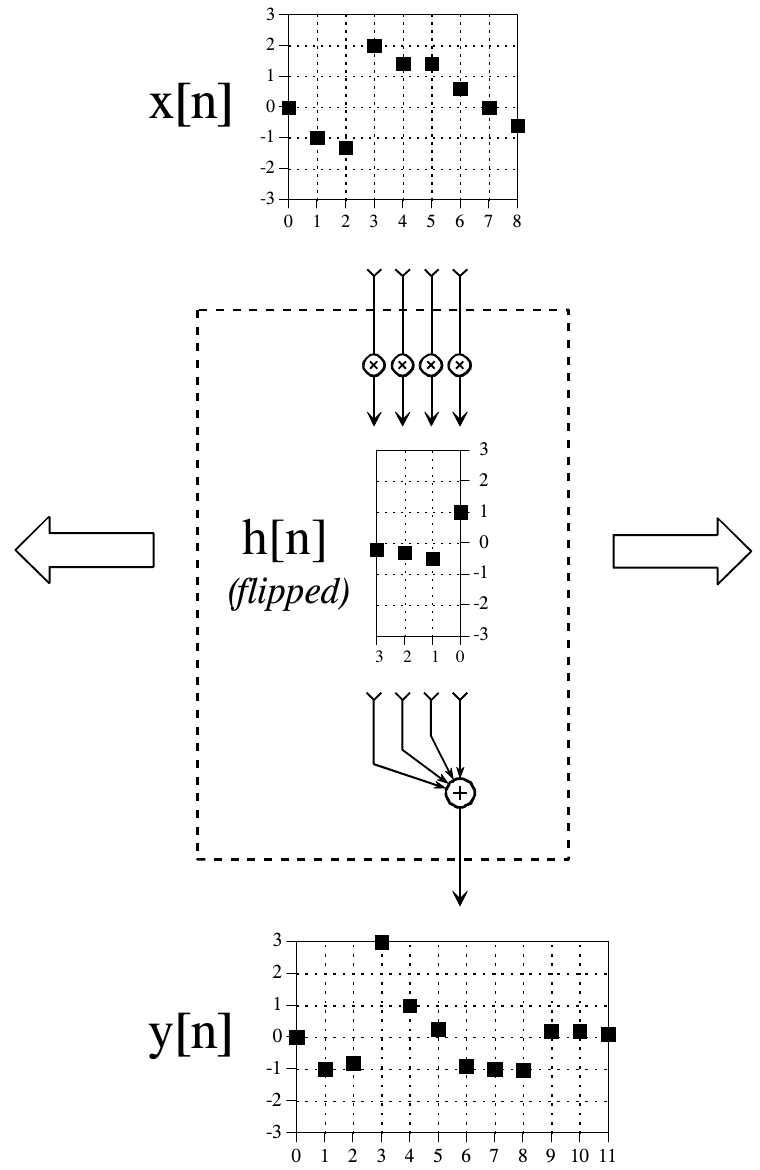
\includegraphics[width=0.633\linewidth,height=0.8\textheight,keepaspectratio]{assets/ch06/fig6-08.png}
\caption*{\textbf{图 6-8　卷积机。}
这是一张流程图，显示输出信号中的每个采样怎样受输入信号和冲激响应的影响。详见正文。
（h{[}n{]} (flipped) = 翻转后的 h{[}n{]}。）}
\end{figure}

冲激响应在卷积机中的排列非常重要：冲激响应是左右翻转的。这样第 0
个采样在最右边，采样序号越大越往左。把它和图 6-5
中正常的冲激响应比较一下，就能理解这种翻转的几何关系。为什么需要翻转？它只是从数学中自然推出来的。冲激响应描述的是输入信号中的每个点怎样影响输出信号。这导致输出信号中的每个点，受到的是输入信号中的点按翻转后的冲激响应加权的影响。

图 6-9
展示了用卷积机计算输出信号中的几个采样。这张图也说明了卷积中一个真正的麻烦。在
(a) 中，卷积机位于最左边，输出对准 y{[}0{]}。在这个位置，它试图从采样
x{[}−3{]}、x{[}−2{]}、x{[}−1{]} 和 x{[}0{]}
接收输入。问题是，其中三个采样 x{[}−3{]}、x{[}−2{]} 和 x{[}−1{]}
并不存在！同样的困境也出现在 (d)
中，卷积机试图接收已定义输入信号右边的采样，即 x{[}9{]}、x{[}10{]} 和
x{[}11{]}。

\begin{figure}[htbp]
\centering
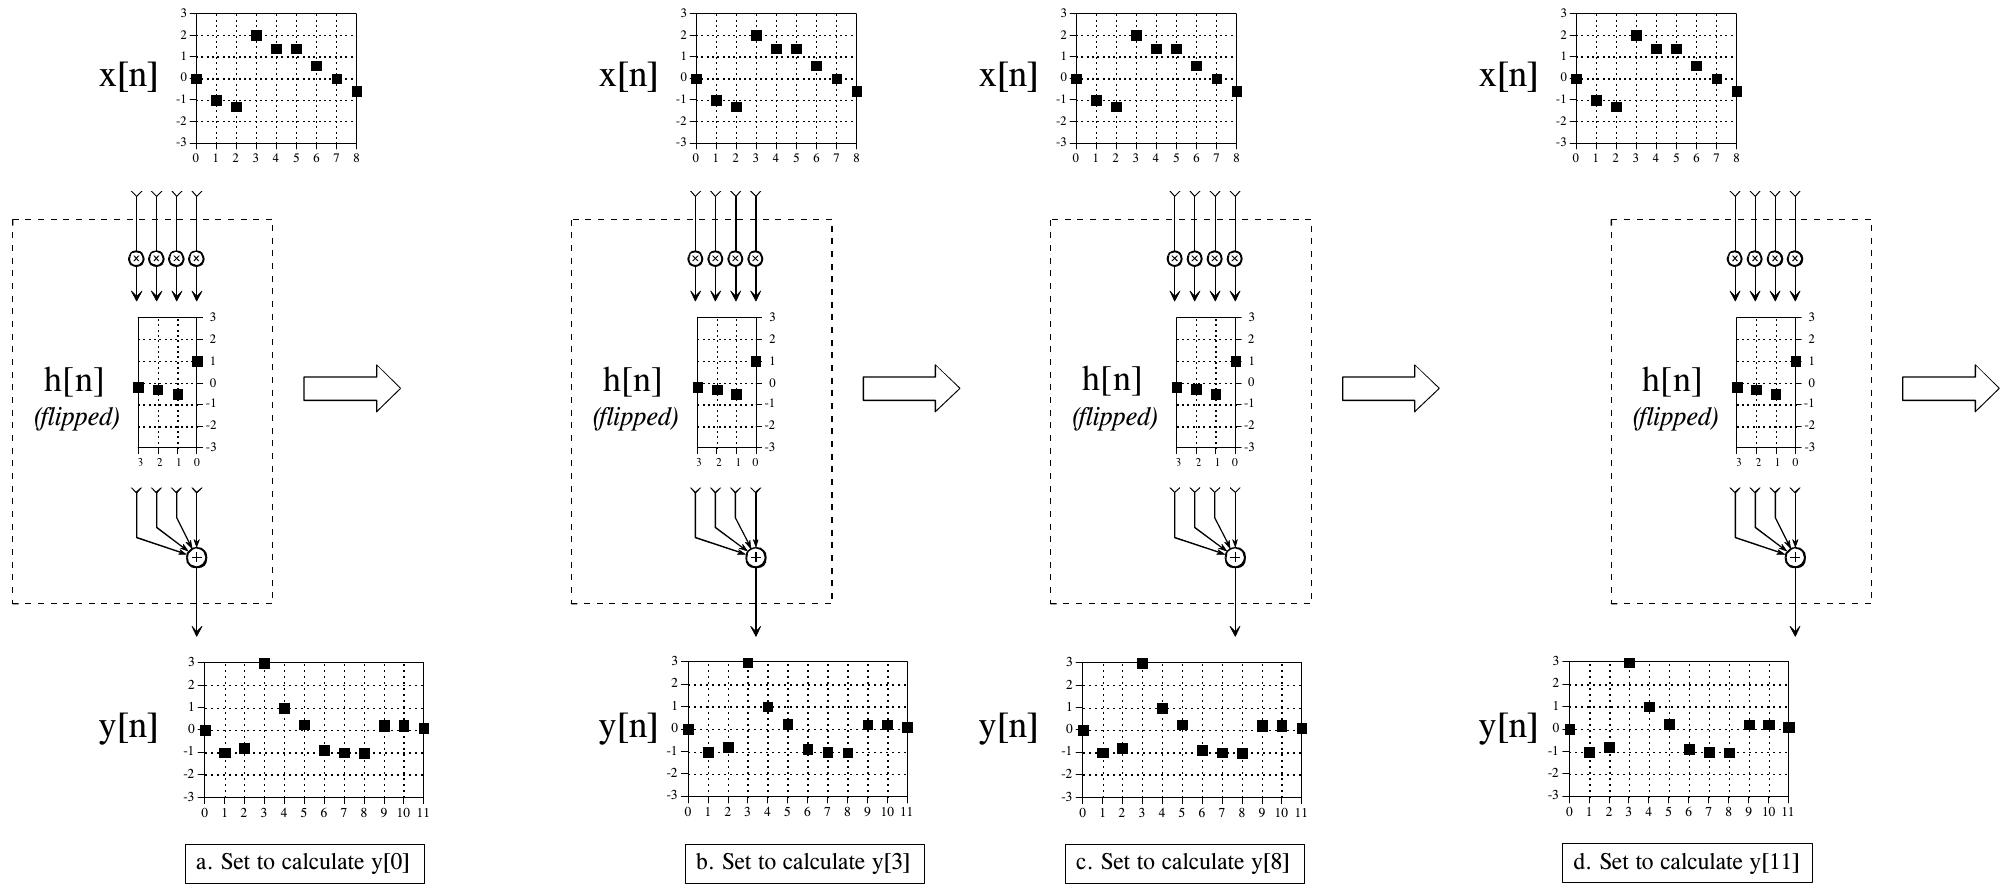
\includegraphics[width=1.000\linewidth,height=0.8\textheight,keepaspectratio]{assets/ch06/fig6-09.png}
\caption*{\textbf{图 6-9　卷积机在工作。} 图 (a)～(d)
显示卷积机分别设置为计算四个不同的输出采样：y{[}0{]}、y{[}3{]}、y{[}8{]}
和 y{[}11{]}。 （a. 设置为计算 y{[}0{]}；b. 设置为计算
y{[}3{]}；c.~设置为计算 y{[}8{]}；d.~设置为计算 y{[}11{]}。原书 (c)(d)
在下一页，这里拼成一张。）}
\end{figure}

处理这个问题的一种办法是把不存在的采样「造」出来。做法是在输入信号的两端添加采样，每个添加的采样值都为零。这叫给信号补零(padding
the signal with
zeros)。卷积机不再试图访问不存在的值，而是收到一个值为零的采样。由于这个零在乘法中被消掉了，结果在数学上和忽略不存在的输入是一样的。

重要的是，输出信号最左边和最右边的采样是基于不完整的信息算出来的。用 DSP
的行话说，冲激响应没有完全浸没(fully
immersed)在输入信号中。如果冲激响应长 M 点，输出信号的前 M−1 个和后 M−1
个采样所依据的信息比中间的采样少。这就像电子电路通电后需要一段时间才能稳定下来。区别在于，这种瞬态(transient)在电子学中很容易忽略，在
DSP 中却非常突出。

图 6-10 展示了这些端点效应(end
effects)可能造成的麻烦。输入信号是一个正弦波加上一个直流分量。目的是去掉信号的直流部分，同时保留正弦波。这需要一个高通滤波器，比如图中所示的冲激响应。问题是，前
30 个和后 30 个点一团糟！要理解这些端区的形状，可以想象输入信号左边补了
30 个零（采样 x{[}−1{]} 到 x{[}−30{]}），右边补了 30 个零（采样
x{[}81{]} 到
x{[}110{]}）。这样输出信号就可以看作对这个更长波形的滤波结果。这种「端点效应」问题在
DSP 中很普遍。一般来说，预计处理后信号开头和结尾的采样会相当没用。

\begin{figure}[htbp]
\centering
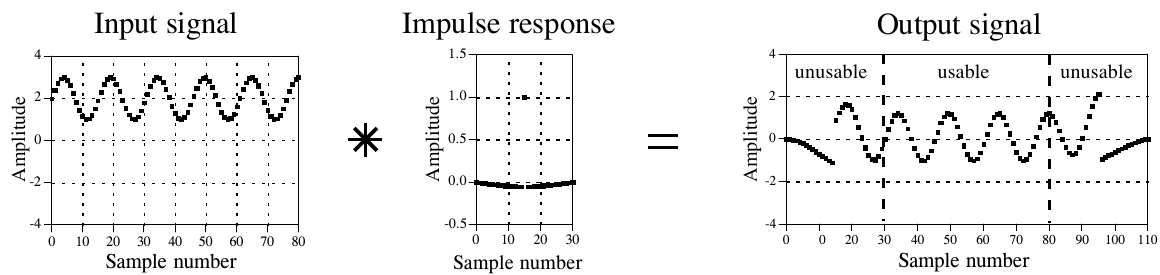
\includegraphics[width=0.967\linewidth,height=0.8\textheight,keepaspectratio]{assets/ch06/fig6-10.png}
\caption*{\textbf{图 6-10　卷积中的端点效应。} 输入信号与 M
点冲激响应卷积时，输出信号的前 M−1 个和后 M−1
个点可能无法使用。本例中，冲激响应是一个高通滤波器，用来去掉输入信号中的直流分量。
（Input signal = 输入信号，Impulse response = 冲激响应，Output signal =
输出信号，usable = 可用，unusable = 不可用。）}
\end{figure}

现在讲数学。以卷积机为指导，我们可以写出卷积的标准公式。如果 x{[}n{]}
是从 0 到 N−1 的 N 点信号，h{[}n{]} 是从 0 到 M−1 的 M
点信号，两者的卷积 \(y[n] = x[n] * h[n]\) 是一个从 0 到 N+M−2 的 N+M−1
点信号，由下式给出：

\textbf{公式 6-1　卷积和。} 这是卷积的正式定义，简写为
\(y[n] = x[n] * h[n]\)。式中 h{[}n{]} 是一个 M 点信号，索引从 0 到 M−1。

\[
y[i] = \sum_{j=0}^{M-1} h[j]\, x[i-j]
\]

这个公式叫卷积和(convolution
sum)。它让输出信号中的每个点都能独立于输出信号中的所有其他点计算出来。索引
i
决定正在计算输出信号的哪个采样，因此对应卷积机的左右位置。在执行卷积的计算机程序中，用一个循环让这个索引遍历输出信号的每个采样。计算其中一个输出采样时，在卷积机内部使用索引
j。当 j 从 0 走到 M−1 时，冲激响应中的每个采样 h{[}j{]}
都乘以输入信号中相应的采样
x{[}i−j{]}。把所有这些乘积相加，就得到正在计算的那个输出采样。仔细研究公式
6-1，直到你完全理解卷积机是怎样实现它的。DSP
的很多内容都基于这个公式。（不要被 \(y[n] = x[n] * h[n]\) 中的 n
搞糊涂。它只是一个占位符，表示某个变量是数组的索引。有时公式写成
\(y[\,] = x[\,] * h[\,]\)，就是为了避免引入一个没有意义的符号。）

表 6-2 是用输出端算法做卷积的程序，直接实现了公式
6-1。这个程序产生的输出信号和前面表 6-1
的输入端算法程序相同。注意这两个程序的主要区别：输入端算法遍历输入信号的每个采样（表
6-1 第 220 行），而输出端算法遍历输出信号的每个采样（表 6-2 第 180
行）。

下面详细说明这个程序的运作。第 180～250 行的 FOR-NEXT 循环用 I\%
作索引，遍历输出信号的每个采样。对其中每个值，由第 200～230
行组成的内层循环计算输出采样 Y{[}I\%{]} 的值。第 190 行把 Y{[}I\%{]}
设为零，让它累加卷积机内部的乘积。第 200～240 行的 FOR-NEXT
循环直接实现了公式 6-1。索引 J\% 遍历冲激响应的每个采样。第 230
行把冲激响应的每个采样 H{[}J\%{]} 与输入信号中相应的采样 X{[}I\%-J\%{]}
相乘，并把结果加到累加器上。

第 230 行从输入信号中取的采样是 X{[}I\%-J\%{]}。第 210 和 220
行防止它超出已定义的数组 X{[}0{]} 到
X{[}80{]}。换句话说，这个程序对输入信号中未定义的采样的处理方式是忽略它们。另一种办法是把输入信号的数组定义为
X{[}-30{]} 到 X{[}110{]}，在真实数据两侧各补 30 个零。第三种办法是把第
180 行的 FOR-NEXT 循环改成从 30 到 80，而不是从 0 到
110。也就是说，程序只计算输出信号中冲激响应完全浸没在输入信号中的那些采样。重要的是，你必须使用这三种技术之一。否则，程序试图读取越界数据时就会崩溃。

\textbf{表 6-2}（注释已译成中文）

\begin{Shaded}
\begin{Highlighting}[]
\NormalTok{100 \textquotesingle{}CONVOLUTION USING THE OUTPUT SIDE ALGORITHM}
\NormalTok{110 \textquotesingle{}}
\NormalTok{120 DIM X[80]                   \textquotesingle{}输入信号，81 点}
\NormalTok{130 DIM H[30]                   \textquotesingle{}冲激响应，31 点}
\NormalTok{140 DIM Y[110]                  \textquotesingle{}输出信号，111 点}
\NormalTok{150 \textquotesingle{}}
\NormalTok{160 GOSUB XXXX                  \textquotesingle{}虚构的子程序，载入 X[ ] 和 H[ ]}
\NormalTok{170 \textquotesingle{}}
\NormalTok{180 FOR I\% = 0 TO 110           \textquotesingle{}遍历 Y[ ] 中的每个点}
\NormalTok{190   Y[I\%] = 0                 \textquotesingle{}把输出数组中的这个采样清零}
\NormalTok{200   FOR J\% = 0 TO 30          \textquotesingle{}遍历 H[ ] 中的每个点}
\NormalTok{210     IF (I\%{-}J\% \textless{} 0)  THEN GOTO 240}
\NormalTok{220     IF (I\%{-}J\% \textgreater{} 80) THEN GOTO 240}
\NormalTok{230     Y(I\%) = Y(I\%) + H(J\%)*X(I\%{-}J\%)}
\NormalTok{240   NEXT J\%}
\NormalTok{250 NEXT I\%}
\NormalTok{260 \textquotesingle{}}
\NormalTok{270 GOSUB XXXX                  \textquotesingle{}虚构的子程序，保存 Y[ ]}
\NormalTok{280 \textquotesingle{}}
\NormalTok{290 END}
\end{Highlighting}
\end{Shaded}

\textbf{C 实现}（完整可编译版本见
\texttt{c/table6-2\_convolve\_output\_side.c}，信号与表 6-1 的 C
版本相同，两者输出逐点一致）：

\begin{Shaded}
\begin{Highlighting}[]
\PreprocessorTok{\#define NX }\DecValTok{81}\PreprocessorTok{                   }\CommentTok{/* 120 DIM X[80]：输入信号 81 点 */}
\PreprocessorTok{\#define NH }\DecValTok{31}\PreprocessorTok{                   }\CommentTok{/* 130 DIM H[30]：冲激响应 31 点 */}
\PreprocessorTok{\#define NY }\OperatorTok{(}\PreprocessorTok{NX }\OperatorTok{+}\PreprocessorTok{ NH }\OperatorTok{{-}}\PreprocessorTok{ }\DecValTok{1}\OperatorTok{)}\PreprocessorTok{        }\CommentTok{/* 140 DIM Y[110]：输出信号 111 点 */}

\CommentTok{/* 输出端算法：公式 6{-}1 的直接实现，每个输出点独立算出 */}
\DataTypeTok{static} \DataTypeTok{void}\NormalTok{ convolve\_output\_side}\OperatorTok{(}\DataTypeTok{const} \DataTypeTok{double} \OperatorTok{*}\NormalTok{x}\OperatorTok{,} \DataTypeTok{const} \DataTypeTok{double} \OperatorTok{*}\NormalTok{h}\OperatorTok{,} \DataTypeTok{double} \OperatorTok{*}\NormalTok{y}\OperatorTok{)}
\OperatorTok{\{}
    \ControlFlowTok{for} \OperatorTok{(}\DataTypeTok{int}\NormalTok{ i }\OperatorTok{=} \DecValTok{0}\OperatorTok{;}\NormalTok{ i }\OperatorTok{\textless{}}\NormalTok{ NY}\OperatorTok{;}\NormalTok{ i}\OperatorTok{++)} \OperatorTok{\{}          \CommentTok{/* 180：遍历输出的每个点 */}
\NormalTok{        y}\OperatorTok{[}\NormalTok{i}\OperatorTok{]} \OperatorTok{=} \FloatTok{0.0}\OperatorTok{;}                         \CommentTok{/* 190：这个输出点的累加器清零 */}
        \ControlFlowTok{for} \OperatorTok{(}\DataTypeTok{int}\NormalTok{ j }\OperatorTok{=} \DecValTok{0}\OperatorTok{;}\NormalTok{ j }\OperatorTok{\textless{}}\NormalTok{ NH}\OperatorTok{;}\NormalTok{ j}\OperatorTok{++)} \OperatorTok{\{}      \CommentTok{/* 200：遍历冲激响应的每个点 */}
            \ControlFlowTok{if} \OperatorTok{(}\NormalTok{i }\OperatorTok{{-}}\NormalTok{ j }\OperatorTok{\textless{}} \DecValTok{0}\OperatorTok{)} \ControlFlowTok{continue}\OperatorTok{;}        \CommentTok{/* 210～220：x[i{-}j] 越界的项不存在，跳过 */}
            \ControlFlowTok{if} \OperatorTok{(}\NormalTok{i }\OperatorTok{{-}}\NormalTok{ j }\OperatorTok{\textgreater{}}\NormalTok{ NX }\OperatorTok{{-}} \DecValTok{1}\OperatorTok{)} \ControlFlowTok{continue}\OperatorTok{;}
\NormalTok{            y}\OperatorTok{[}\NormalTok{i}\OperatorTok{]} \OperatorTok{+=}\NormalTok{ h}\OperatorTok{[}\NormalTok{j}\OperatorTok{]} \OperatorTok{*}\NormalTok{ x}\OperatorTok{[}\NormalTok{i }\OperatorTok{{-}}\NormalTok{ j}\OperatorTok{];}        \CommentTok{/* 230：h[j]·x[i{-}j]，即卷积机里的一次乘加 */}
        \OperatorTok{\}}
    \OperatorTok{\}}
\OperatorTok{\}}
\end{Highlighting}
\end{Shaded}

\section{输入的加权求和}

线性系统的特性完全由它的冲激响应描述。这是输入端算法的基础：输入信号中的每个点都给输出信号贡献一个经过缩放和平移的冲激响应。由此推出的数学结果就是输出端算法：输出信号中的每个点都从输入信号的许多点接收贡献，这些点乘以翻转后的冲激响应。这些虽然都对，但并没有完整说明卷积为什么在信号处理中这么重要。

回头看图 6-8
中的卷积机，先别管虚线框里的信号是冲激响应。把它看作一组碰巧嵌在流程图里的加权系数(weighing
coefficients)。从这个角度看，输出信号中的每个采样都等于输入的加权和(sum
of weighted
inputs)。输出中的每个采样受输入信号中一片区域的采样影响，这片区域由选定的加权系数决定。例如，设想有十个加权系数，每个都是十分之一。这样输出信号中的每个采样就是输入中十个采样的平均值。

更进一步，加权系数并不一定只能在正在计算的输出采样的左边。例如，图 6-8
显示 y{[}6{]} 是由 x{[}3{]}、x{[}4{]}、x{[}5{]} 和 x{[}6{]}
算出来的。把卷积机看作输入的加权和时，加权系数可以选得围绕输出采样对称。例如，y{[}6{]}
可以从 x{[}4{]}、x{[}5{]}、x{[}6{]}、x{[}7{]} 和 x{[}8{]}
接收贡献。按照图 6-8 中同样的索引记法，这五个输入的加权系数存放在
h{[}2{]}、h{[}1{]}、h{[}0{]}、h{[}−1{]} 和 h{[}−2{]}
中。换句话说，对应我们所选的对称加权系数的冲激响应，需要使用负索引。下一章我们会回到这个问题。

从数学上说，这里只有一个概念：公式 6-1
定义的卷积。然而，科学和工程问题从两个截然不同的方向接近这同一个概念。有时你会想从系统的冲激响应长什么样来思考系统；另一些时候，你会把系统理解为一组加权系数。你需要熟悉这两种视角，以及怎样在它们之间切换。

% !TEX root = ../main.tex
% 本文件由 build-tex.sh 从 07-DSP指南-第7章中译.md 生成，改内容请改 md 后重新生成

\chapter{卷积的性质}\label{ch-07}

线性系统的特性完全由系统的冲激响应决定，而这种决定关系由卷积的数学来描述。这是许多信号处理技术的基础。例如：数字滤波器是通过设计一个合适的冲激响应做出来的；雷达通过分析测得的冲激响应来发现敌机；长途电话中的回声抑制，是造出一个冲激响应来抵消混响的冲激响应。这样的例子数不胜数。本章从几个方面展开讲卷积的性质和用法。第一，讨论几种常见的冲激响应。第二，介绍怎样处理线性系统的级联与并联组合。第三，引入相关(correlation)这一技术。第四，考察卷积的一个棘手问题：用常规算法和计算机，计算时间可能长得无法接受。

\section{常见的冲激响应}

\subsection{冲激函数}

最简单的冲激响应就是一个冲激函数(delta function)，如图 7-1a
所示。也就是说，输入一个冲激，输出一个一模一样的冲激。这意味着所有信号都原封不动地通过这个系统。任何信号与冲激函数卷积，结果都和原信号完全相同。写成数学式：

\textbf{公式
7-1}　冲激函数是卷积的单位元。任何信号与冲激函数卷积都保持不变。

\[x[n] * \delta[n] = x[n]\]

这个性质使冲激函数成为卷积的单位元(identity)。这就像零是加法的单位元（\(a + 0 = a\)），一是乘法的单位元（\(a \times 1 = a\)）。乍一看，这种系统好像平淡无奇、没什么意思。并非如此！这种系统正是数据存储、通信和测量追求的理想。DSP
有很大一部分工作，就是让信息通过系统时不发生改变、不受损伤。

图 7-1b
对冲激函数形式的冲激响应稍作改动。如果把冲激函数的幅度变大或变小，得到的系统就分别是放大器(amplifier)或衰减器(attenuator)。写成公式，k
大于一时是放大，k 小于一时是衰减：

\textbf{公式
7-2}　放大或衰减的系统，其冲激响应是一个缩放过的冲激函数。式中 k
决定放大或衰减的倍数。

\[x[n] * k\,\delta[n] = k\,x[n]\]

图 7-1c
中的冲激响应是一个平移过的冲激函数。由此得到的系统会在输入和输出信号之间引入同样大小的平移。根据平移方向的不同，这可以叫做信号延迟(delay)或信号超前(advance)。用参数
s 表示平移量，可以写成公式：

\textbf{公式
7-3}　输入与输出信号之间的相对平移，对应一个平移过的冲激函数作为冲激响应。式中变量
s 决定平移量。

\[x[n] * \delta[n+s] = x[n+s]\]

科学和工程中，一个信号是另一个信号平移版本的情况比比皆是。例如，想想一个远方的太空探测器发出的无线电信号，以及地球上收到的相应信号。无线电波传播这段距离需要时间，因此发出的信号和收到的信号之间有一段延迟。在生物学中，相邻神经细胞里的电信号互为平移版本，平移量由动作电位(action
potential)穿过连接两者的突触(synaptic junction)所需的时间决定。

图 7-1d
的冲激响应由一个冲激函数加上一个平移并缩放过的冲激函数组成。根据叠加原理，这个系统的输出就是输入信号加上输入信号的一个延迟版本，也就是回声(echo)。回声在许多
DSP
应用中都很重要。加入回声是让录音听起来自然悦耳的关键一环。雷达和声呐靠分析回声来发现飞机和潜艇。地球物理学家用回声找石油。回声在电话网络中也非常重要，因为你要避免它。

\begin{figure}[htbp]
\centering
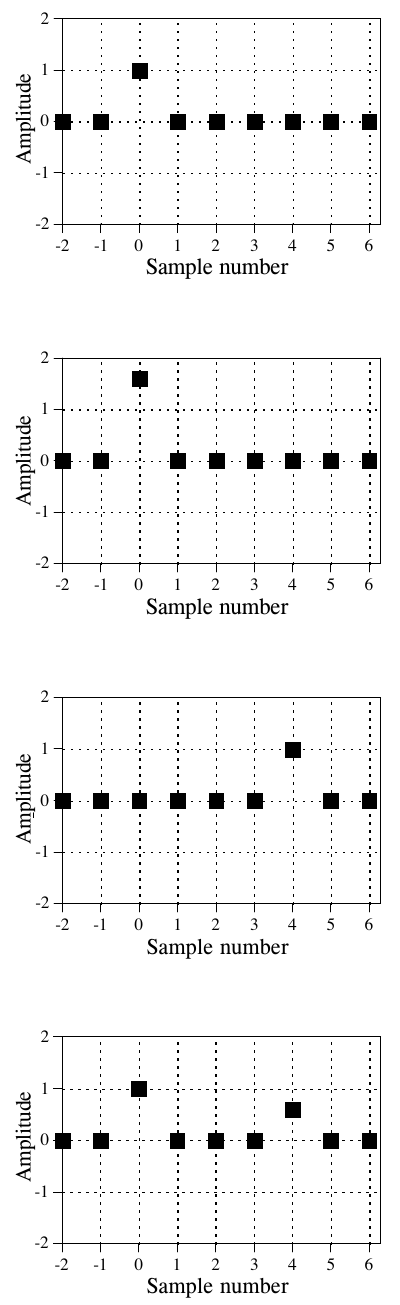
\includegraphics[width=0.333\linewidth,height=0.8\textheight,keepaspectratio]{assets/ch07/fig7-01.png}
\caption*{\textbf{图 7-1　用平移和缩放过的冲激函数构成的简单冲激响应。}
从上到下四个子图依次为： - \textbf{a.
恒等(Identity)}：冲激函数是卷积的单位元。信号与冲激函数卷积后保持不变。这正是传输或存储信号的系统追求的目标。
- \textbf{b. 放大与衰减(Amplification \&
Attenuation)}：把冲激函数的幅度变大或变小，就得到放大或衰减的冲激响应。图中这个冲激响应把信号放大
1.6 倍。 -
\textbf{c.~平移(Shift)}：平移冲激函数，输入与输出信号之间就产生相应的平移。根据方向不同，可以叫延迟或超前。图中这个冲激响应把信号延迟
4 个采样。 -
\textbf{d.~回声(Echo)}：冲激函数加上一个平移并缩放过的冲激函数，结果是在原信号上叠加一个回声。本例中回声延迟
4 个采样，幅度是原信号的 60\%。}
\end{figure}

（Amplitude = 幅度，Sample number =
采样序号。原书这四段说明排在各子图左侧，裁图时已去掉，译文见上。）

\subsection{类似微积分的运算}

卷积能以类似积分和微分的方式改变离散信号。由于''导数''和''积分''这两个词专指对连续信号的运算，它们的离散对应物另有名称。模仿一阶导数的离散运算叫一阶差分(first
difference)。同样，积分的离散形式叫累加和(running
sum)。也常听人把这两种运算叫做离散导数(discrete
derivative)和离散积分(discrete
integral)，不过数学家听到这种不正式的叫法会皱眉头。

图 7-2 给出了实现一阶差分和累加和的冲激响应。图 7-3
是使用这两种运算的一个例子。在 7-3a
中，原信号由几段斜率各不相同的部分组成。把这个信号与一阶差分的冲激响应卷积，得到图
7-3b
的信号。和一阶导数一样，一阶差分信号中每个点的幅度，等于原信号中对应位置的斜率。累加和是一阶差分的逆运算。也就是说，把
(b) 中的信号与累加和的冲激响应卷积，就得到 (a) 中的信号。

这些冲激响应很简单，实现它们通常用不着完整的卷积程序。不如换一种方式去想：输出信号中的每个采样，是输入中若干采样的加权和。例如，一阶差分可以这样算：

\textbf{公式 7-4}　一阶差分的计算。式中 x{[}n{]} 是原信号，y{[}n{]}
是一阶差分。

\[y[n] = x[n] - x[n-1]\]

也就是说，输出信号的每个采样，等于输入信号中相邻两个采样之差。例如
\(y[40] = x[40] - x[39]\)。需要说明的是，这不是定义离散导数的唯一方法。另一种常见做法是围绕所考察的点对称地定义斜率，比如
\(y[n] = (x[n+1] - x[n-1])/2\)。

\begin{figure}[htbp]
\centering
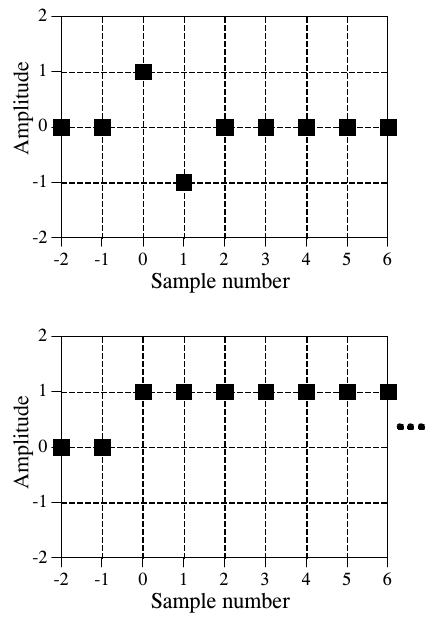
\includegraphics[width=0.362\linewidth,height=0.8\textheight,keepaspectratio]{assets/ch07/fig7-02.png}
\caption*{\textbf{图 7-2　模仿微积分运算的冲激响应。} 上下两个子图依次为： -
\textbf{a. 一阶差分(First
Difference)}：这是一阶导数的离散版本。输出信号的每个采样等于输入信号中相邻采样之差。换句话说，输出信号就是输入信号的斜率。
- \textbf{b. 累加和(Running
Sum)}：这是积分的离散版本。输出信号的每个采样等于输入信号中它左边所有采样之和。注意这个冲激响应一直延伸到无穷远，这是个相当讨厌的特点。}
\end{figure}

（Amplitude = 幅度，Sample number =
采样序号。原书说明排在子图左侧，裁图时已去掉，译文见上。）

\begin{figure}[htbp]
\centering
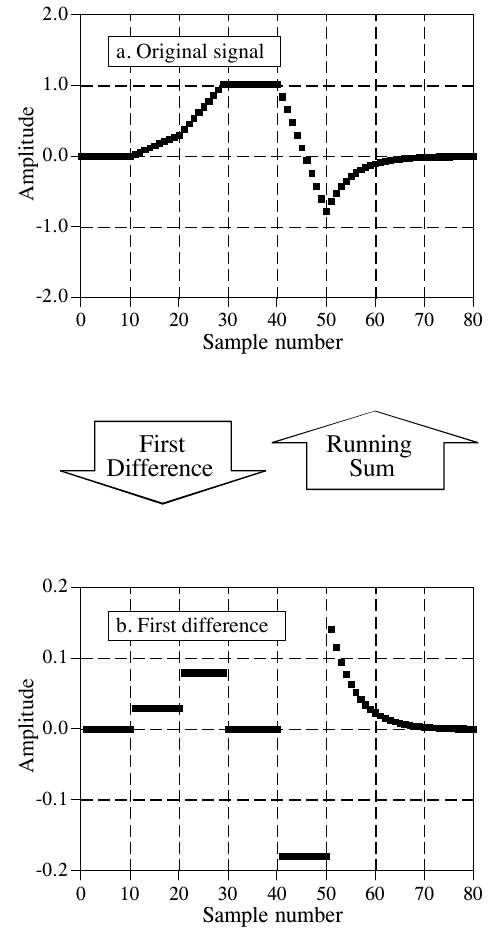
\includegraphics[width=0.412\linewidth,height=0.8\textheight,keepaspectratio]{assets/ch07/fig7-03.png}
\caption*{\textbf{图 7-3　类似微积分运算的例子。} (b) 中的信号是 (a)
中信号的一阶差分；相应地，(a) 中的信号是 (b)
中信号的累加和。这些处理方法用于离散信号，就像微分和积分用于连续信号一样。
（a. Original signal = 原信号；b. First difference =
一阶差分。中间两个箭头：First Difference = 一阶差分（向下），Running Sum
= 累加和（向上）。原书图注把第二个 ``signal in'' 误印成 ``signal
is''。）}
\end{figure}

用同样的思路，累加和中的每个采样，可以通过把原信号中该采样位置左边的所有点加起来求得。例如，若
y{[}n{]} 是 x{[}n{]} 的累加和，那么采样 y{[}40{]} 由 x{[}0{]} 到
x{[}40{]} 相加得到；同样，y{[}41{]} 由 x{[}0{]} 到 x{[}41{]}
相加得到。当然，这样算累加和效率很低。例如，如果 y{[}40{]}
已经算出来了，那么 y{[}41{]}
只需一次加法就能算出：\(y[41] = x[41] + y[40]\)。写成公式：

\textbf{公式 7-5}　累加和的计算。式中 x{[}n{]} 是原信号，y{[}n{]}
是累加和。

\[y[n] = x[n] + y[n-1]\]

这类关系式叫做递推方程(recursion equation)或差分方程(difference
equation)。第 19 章会再讲到它们。眼下要理解的重点是：这些关系式与使用图
7-2 冲激响应的卷积完全等价。表 7-1 给出了实现这些类似微积分运算的程序。

\textbf{表 7-1}　计算一阶差分和累加和的程序。原信号存放在 X{[} {]}
中，处理后的信号（一阶差分或累加和）存放在 Y{[} {]}
中。两个数组的下标都从 0 到
N\%−1。（注释已译成中文，原书没有注释的行照原样保留。）

\begin{Shaded}
\begin{Highlighting}[]
\NormalTok{100 \textquotesingle{}Calculation of the First Difference      100 \textquotesingle{}Calculation of the running sum}
\NormalTok{110 Y[0] = 0                                  110 Y[0] = X[0]}
\NormalTok{110 FOR I\% = 1 TO N\%{-}1                        120 FOR I\% = 1 TO N\%{-}1}
\NormalTok{120   Y[I\%] = X[I\%] {-} Y[I\%{-}1]                 120   Y[I\%] = Y[I\%{-}1] + X[I\%]}
\NormalTok{130 NEXT I\%                                   130 NEXT I\%}
\end{Highlighting}
\end{Shaded}

\begin{quote}
\textbf{译注：} 左边一阶差分程序第 120 行原书印成
\texttt{Y{[}I\%{]}\ =\ X{[}I\%{]}\ -\ Y{[}I\%-1{]}}，这是笔误。按公式
7-4 应为
\texttt{Y{[}I\%{]}\ =\ X{[}I\%{]}\ -\ X{[}I\%-1{]}}；照原样执行，减去的是上一个输出而不是上一个输入，得到的不是一阶差分。另外两段程序的行号都有重复（左边两个
110，右边两个 120），也是排版错误，不影响理解。
\end{quote}

\textbf{C 实现}（完整可编译版本见
\texttt{c/table7-1\_difference\_running\_sum.c}，其中按图 7-3a
的形状生成原信号，先求一阶差分，再对差分求累加和，检查能否还原原信号）：

\begin{Shaded}
\begin{Highlighting}[]
\CommentTok{/* 左段程序：一阶差分，y[n] = x[n] {-} x[n{-}1]（公式 7{-}4） */}
\DataTypeTok{static} \DataTypeTok{void}\NormalTok{ first\_difference}\OperatorTok{(}\DataTypeTok{const} \DataTypeTok{double} \OperatorTok{*}\NormalTok{x}\OperatorTok{,} \DataTypeTok{double} \OperatorTok{*}\NormalTok{y}\OperatorTok{)}
\OperatorTok{\{}
\NormalTok{    y}\OperatorTok{[}\DecValTok{0}\OperatorTok{]} \OperatorTok{=} \FloatTok{0.0}\OperatorTok{;}                             \CommentTok{/* 110：第 0 点左边没有点，差分定为 0 */}
    \ControlFlowTok{for} \OperatorTok{(}\DataTypeTok{int}\NormalTok{ i }\OperatorTok{=} \DecValTok{1}\OperatorTok{;}\NormalTok{ i }\OperatorTok{\textless{}}\NormalTok{ N}\OperatorTok{;}\NormalTok{ i}\OperatorTok{++)}             \CommentTok{/* 110（原书重号）：FOR I\% = 1 TO N\%{-}1 */}
\NormalTok{        y}\OperatorTok{[}\NormalTok{i}\OperatorTok{]} \OperatorTok{=}\NormalTok{ x}\OperatorTok{[}\NormalTok{i}\OperatorTok{]} \OperatorTok{{-}}\NormalTok{ x}\OperatorTok{[}\NormalTok{i }\OperatorTok{{-}} \DecValTok{1}\OperatorTok{];}             \CommentTok{/* 120：按公式 7{-}4，原书误印为 X[I\%] {-} Y[I\%{-}1] */}
\OperatorTok{\}}

\CommentTok{/* 右段程序：累加和，y[n] = x[n] + y[n{-}1]（公式 7{-}5） */}
\DataTypeTok{static} \DataTypeTok{void}\NormalTok{ running\_sum}\OperatorTok{(}\DataTypeTok{const} \DataTypeTok{double} \OperatorTok{*}\NormalTok{x}\OperatorTok{,} \DataTypeTok{double} \OperatorTok{*}\NormalTok{y}\OperatorTok{)}
\OperatorTok{\{}
\NormalTok{    y}\OperatorTok{[}\DecValTok{0}\OperatorTok{]} \OperatorTok{=}\NormalTok{ x}\OperatorTok{[}\DecValTok{0}\OperatorTok{];}                            \CommentTok{/* 110：第 0 点的累加和就是它自己 */}
    \ControlFlowTok{for} \OperatorTok{(}\DataTypeTok{int}\NormalTok{ i }\OperatorTok{=} \DecValTok{1}\OperatorTok{;}\NormalTok{ i }\OperatorTok{\textless{}}\NormalTok{ N}\OperatorTok{;}\NormalTok{ i}\OperatorTok{++)}             \CommentTok{/* 120：FOR I\% = 1 TO N\%{-}1 */}
\NormalTok{        y}\OperatorTok{[}\NormalTok{i}\OperatorTok{]} \OperatorTok{=}\NormalTok{ y}\OperatorTok{[}\NormalTok{i }\OperatorTok{{-}} \DecValTok{1}\OperatorTok{]} \OperatorTok{+}\NormalTok{ x}\OperatorTok{[}\NormalTok{i}\OperatorTok{];}             \CommentTok{/* 120（原书重号）：前一点的累加和再加上当前点 */}
\OperatorTok{\}}
\end{Highlighting}
\end{Shaded}

运行结果：一阶差分在各段分别是 0、0.03、0.07、0、−0.18，第 51 点跳到约
0.145 后按指数衰减，形状与图 7-3b 一致；再对它求累加和，81
个点与原信号的最大偏差为 0，印证了''累加和是一阶差分的逆运算''。

\subsection{低通和高通滤波器}

数字滤波器的设计在后面的章节中会详细讲。眼下只要了解低通(low-pass)和高通(high-pass)滤波器核（filter
kernel，滤波器冲激响应的另一个名字）的大致形状就够了。图 7-4
给出了几种常见的低通滤波器核。一般来说，低通滤波器核由一组相邻的正值点组成。这使得输出信号的每个采样，都是输入信号中许多相邻点的加权平均。这种平均使信号变平滑，从而去掉高频成分。如
(c) 中的 sinc
函数所示，有些低通滤波器核的尾部带有少量负值采样。和模拟电子学中一样，数字低通滤波器用于降噪、信号分离、波形整形等。

\begin{figure}[htbp]
\centering
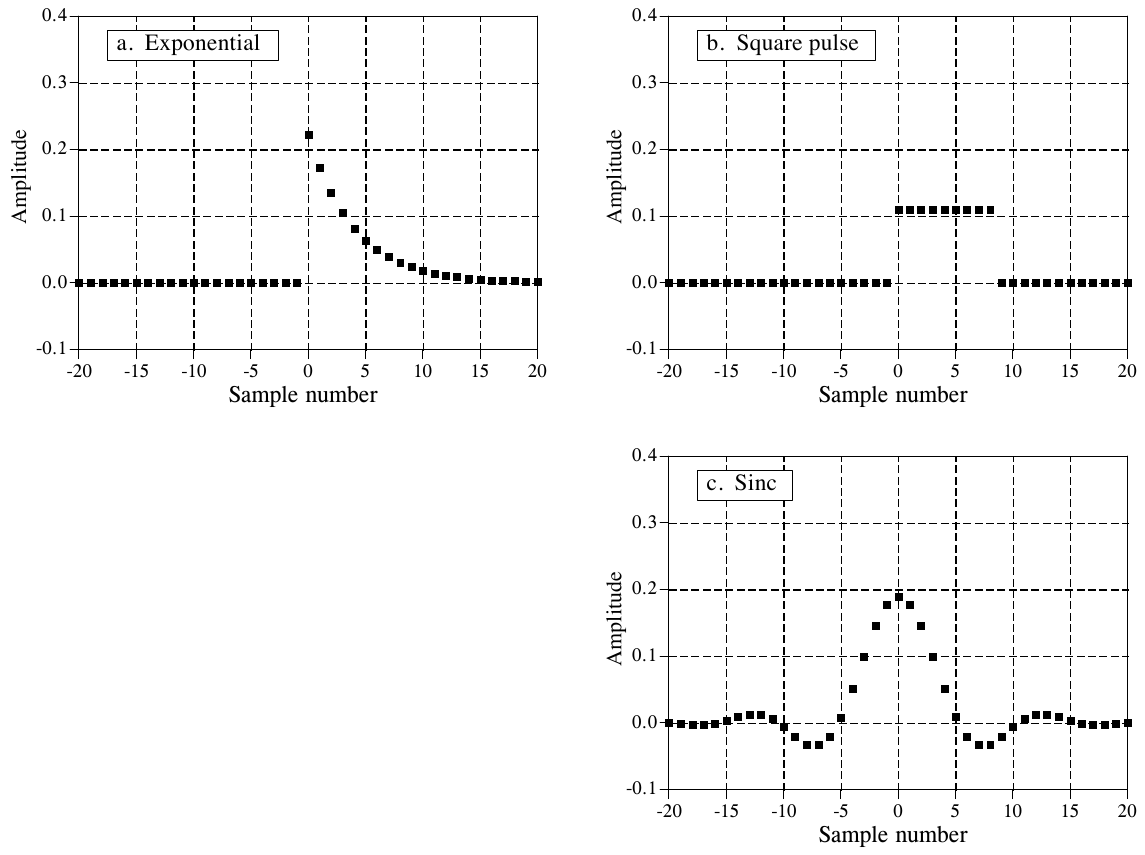
\includegraphics[width=0.954\linewidth,height=0.8\textheight,keepaspectratio]{assets/ch07/fig7-04.png}
\caption*{\textbf{图 7-4　典型的低通滤波器核。}
低通滤波器核由一组相邻的正值点构成，对信号起平均（平滑）作用。后面的章节会讲到，这几种滤波器核各自最适合某种用途。(a)
指数型是最简单的递归滤波器(recursive filter)。(b)
矩形脉冲最擅长在降低噪声的同时保持边缘锐利。(c) sinc 函数是形如
\(\sin(x)/x\) 的曲线，用于把一个频带与另一个频带分开。 （a. Exponential
= 指数型；b. Square pulse = 方波脉冲（即矩形脉冲）；c.~Sinc = sinc
函数。Amplitude = 幅度，Sample number = 采样序号。）}
\end{figure}

把滤波器核变宽或变窄，就能改变滤波器的截止频率(cutoff
frequency)。如果一个低通滤波器在直流（DC，即零频率）处的增益为一，那么它冲激响应中所有点的和必须等于一。如
(a) 和 (c)
所示，有些滤波器核理论上会一直延伸到无穷远，而永远不降到零。实际使用时，尾部在一定数量的采样之后被截断，这样就能用有限个点来表示它。不然怎么存进计算机呢？

图 7-5 给出了三种常见的高通滤波器核，它们由图 7-4
中对应的低通滤波器核推导而来。这是滤波器设计中的一个常用策略：先设计一个低通滤波器，再把它变换成你需要的类型，高通、带通(band-pass)、带阻(band-reject)等等。要理解从低通到高通的变换，记住：冲激函数形式的冲激响应让整个信号通过，而低通冲激响应只让低频成分通过。根据叠加原理，由''冲激函数减去低通滤波器核''构成的滤波器核，会让''整个信号减去低频成分''通过。高通滤波器就这样诞生了！如图
7-5 所示，冲激函数通常加在对称中心处；如果滤波器核不对称，就加在第 0
个采样处。高通滤波器在直流（零频率）处的增益为零，这是通过让滤波器核所有点的和等于零来实现的。

\begin{figure}[htbp]
\centering
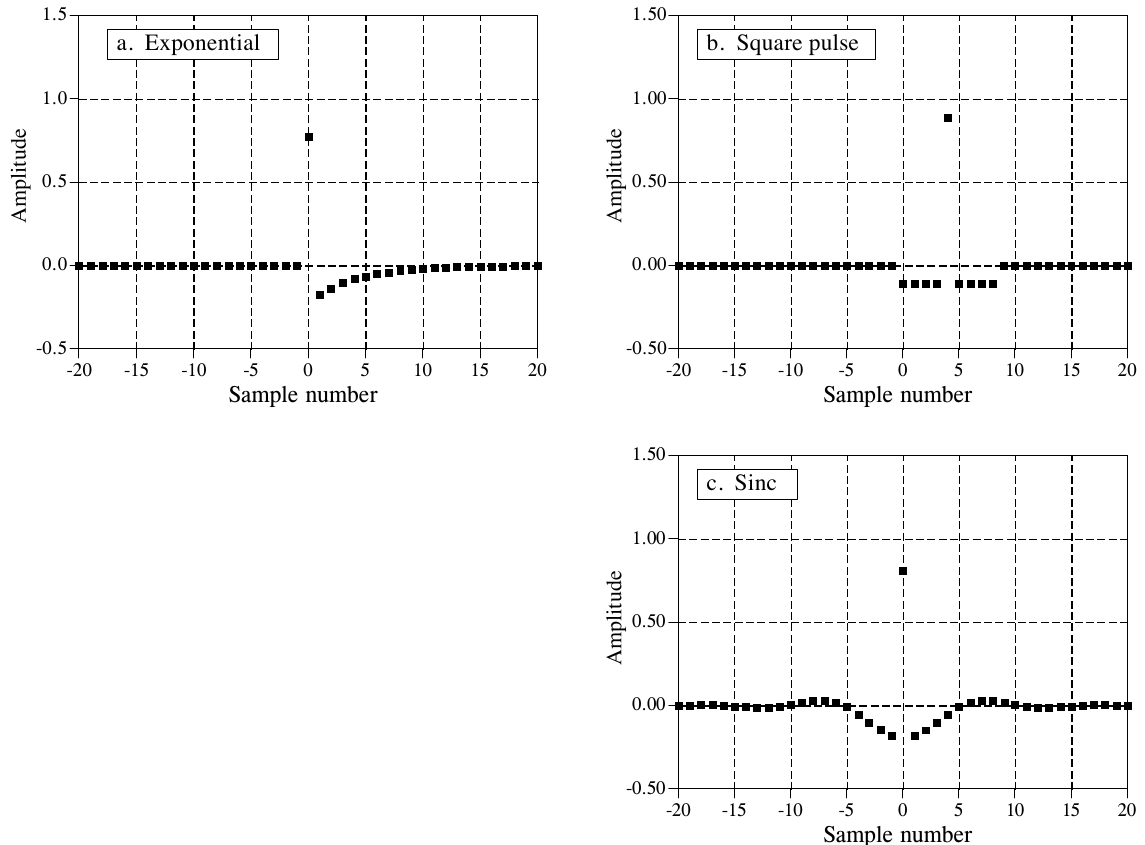
\includegraphics[width=0.954\linewidth,height=0.8\textheight,keepaspectratio]{assets/ch07/fig7-05.png}
\caption*{\textbf{图 7-5　典型的高通滤波器核。} 它们由冲激函数减去图 7-4
中对应的低通滤波器核得到。高通滤波器核的显著特点是：一个尖峰，周围是许多相邻的负值采样。
（a. Exponential = 指数型；b. Square pulse = 方波脉冲；c.~Sinc = sinc
函数。Amplitude = 幅度，Sample number = 采样序号。）}
\end{figure}

\subsection{因果信号与非因果信号}

设想一个简单的模拟电子电路。给输入加一个短脉冲，就会在输出看到一个响应。这正是我们的宇宙赖以存在的那种因果关系。有一点我们可以肯定：任何结果都必须发生在原因之后。这是我们称为''时间''的东西的一个基本特征。现在拿它和一个把输入信号变成输出信号的
DSP
系统比较，两个信号都以数组的形式存放在计算机里。如果这个系统模仿的是真实世界的系统，它就必须和真实世界一样遵守因果律。例如，输入信号第
8 个采样的值，只能影响输出信号第 8
个及以后的采样。以这种方式工作的系统叫因果系统(causal
system)。当然，数字处理不一定非得这样运作。既然输入和输出信号都是存放在计算机里的数组，任何一个输入值都可以影响任何一个输出值。

如图 7-6
的例子所示，因果系统的冲激响应在所有负序号采样处的值都必须为零。可以从卷积的输入端视角来想：要满足因果性，输入信号中第
n 个采样处的冲激，只能影响输出信号中序号大于等于 n
的那些点。在通常用法中，``因果''一词适用于任何负序号采样全为零的信号，不论它是不是冲激响应。

\begin{figure}[htbp]
\centering
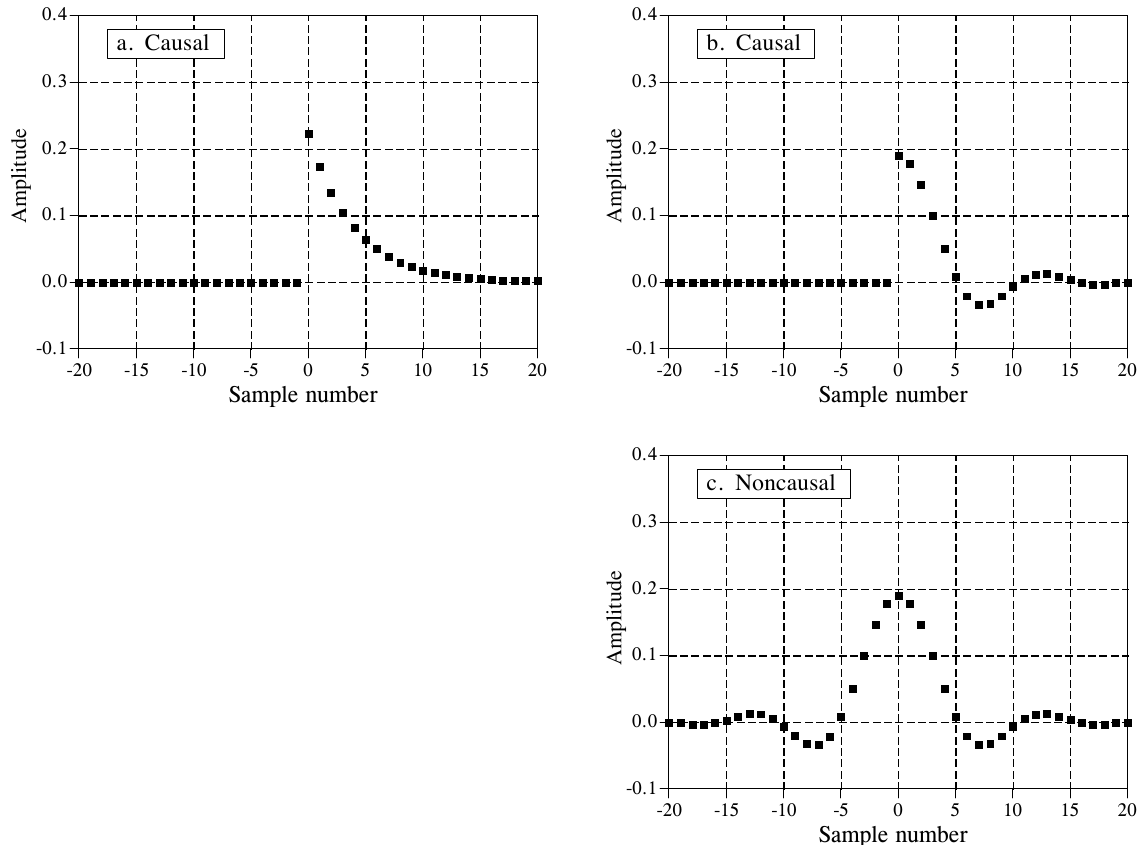
\includegraphics[width=0.954\linewidth,height=0.8\textheight,keepaspectratio]{assets/ch07/fig7-06.png}
\caption*{\textbf{图 7-6　因果信号的例子。}
一个冲激响应（或任何信号），如果所有负序号采样的值都为零，就称为因果的(causal)。这里给出了三个例子。任何点数有限的非因果信号，只要平移一下就能变成因果信号。
（a. Causal = 因果；b. Causal = 因果；c.~Noncausal = 非因果。Amplitude =
幅度，Sample number = 采样序号。）}
\end{figure}

\subsection{零相位、线性相位与非线性相位}

如图 7-7 所示，一个信号如果关于第 0 个采样左右对称，就称它是零相位(zero
phase)的。如果它左右对称、但对称轴不在零点，就称它是线性相位(linear
phase)的。这意味着任何线性相位信号，只要向左或向右平移，就能变成零相位信号。最后，一个信号如果没有左右对称性，就称它是非线性相位(nonlinear
phase)的。

\begin{figure}[htbp]
\centering
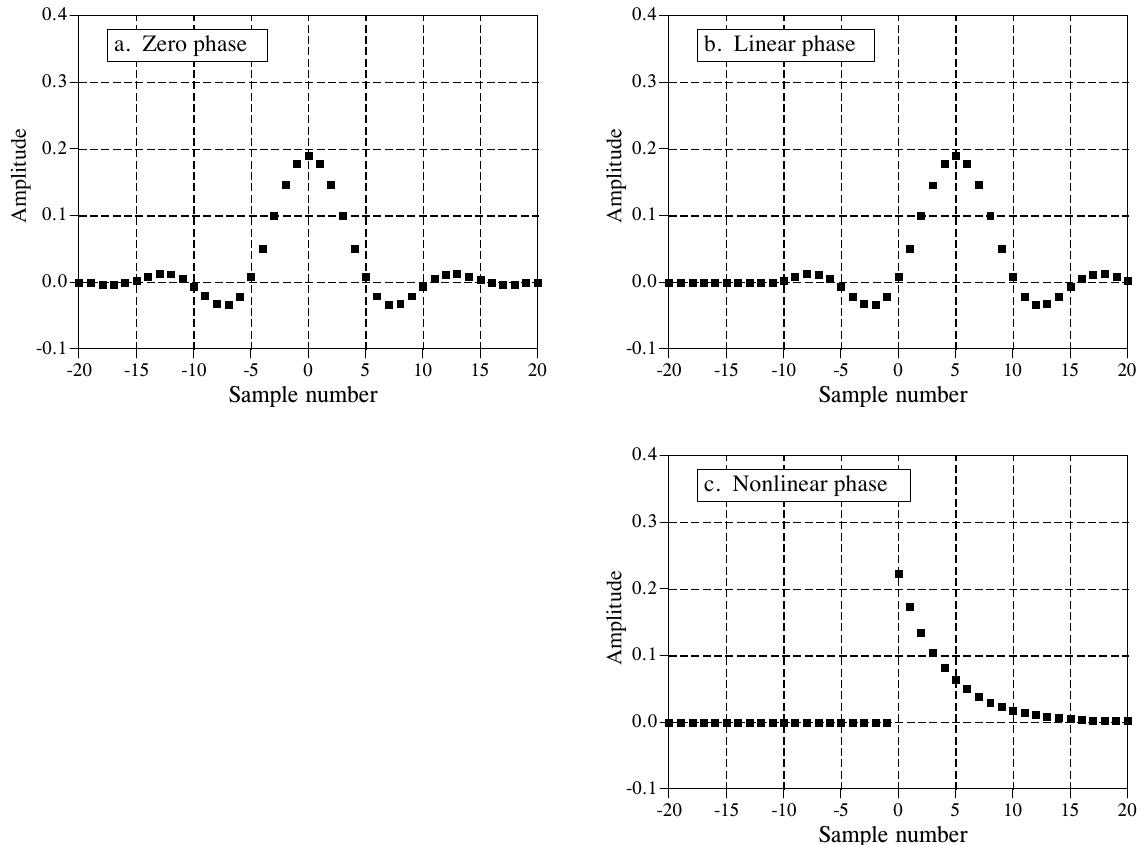
\includegraphics[width=0.954\linewidth,height=0.8\textheight,keepaspectratio]{assets/ch07/fig7-07.png}
\caption*{\textbf{图 7-7　相位线性的例子。}
左右对称的信号称为线性相位的。如果对称轴恰好在第 0
个采样处，还称它是零相位的。任何线性相位信号只要平移就能变成零相位信号。没有左右对称性的信号称为非线性相位的。别把这些术语和''线性系统''里的''线性''混为一谈，它们是完全不同的概念。
（a. Zero phase = 零相位；b. Linear phase = 线性相位；c.~Nonlinear phase
= 非线性相位。Amplitude = 幅度，Sample number = 采样序号。）}
\end{figure}

你大概会觉得，这些名字和它们的定义好像对不上。相位和对称有什么关系？答案在频谱(frequency
spectrum)里，后面的章节会细讲。简单地说，任何信号的频谱都由两部分组成：幅度(magnitude)和相位(phase)。关于零点对称的信号，其频谱的相位为零。同样，关于某个非零点对称的信号，其频谱的相位是一条直线，即线性相位。最后，不对称的信号，其频谱的相位不是直线，即非线性相位。

关于''线性相位''和''非线性相位''这两个容易混淆的术语，要特别说明一下。它们和前几章讨论的系统线性(system
linearity)有什么关系？毫无关系！系统线性是一个宽泛的概念，几乎整个 DSP
都建立在它之上（叠加性、齐次性、可加性等）。线性相位和非线性相位的意思只是相位是不是一条直线。事实上，一个系统必须是线性的，才谈得上它的相位是零、线性还是非线性。

\section{数学性质}

\subsection{交换律}

卷积的交换律(commutative property)写成数学式是：

\textbf{公式 7-6}　卷积的交换律。它说明两个信号卷积的先后顺序可以交换。

\[a[n] * b[n] = b[n] * a[n]\]

用文字说，两个信号谁先谁后卷积没有区别，结果完全相同。如图 7-8
所示，这在系统理论中有一个奇怪的含义：在任何线性系统中，输入信号和系统的冲激响应可以互换，而输出信号不变。这很有意思，但通常没有任何物理意义。输入信号和冲激响应是截然不同的东西。数学允许你做某件事，不代表做这件事有意义。打个比方，假设你的收入是：10
美元/小时 × 2000 小时/年 = 20000 美元/年。乘法交换律告诉你，每年只工作
10 小时、时薪 2000
美元，也能拿到同样的年薪。去说服你老板这有道理试试！尽管如此，交换律在
DSP 中被大量用于推导公式，就像在普通代数里一样。

\begin{figure}[htbp]
\centering
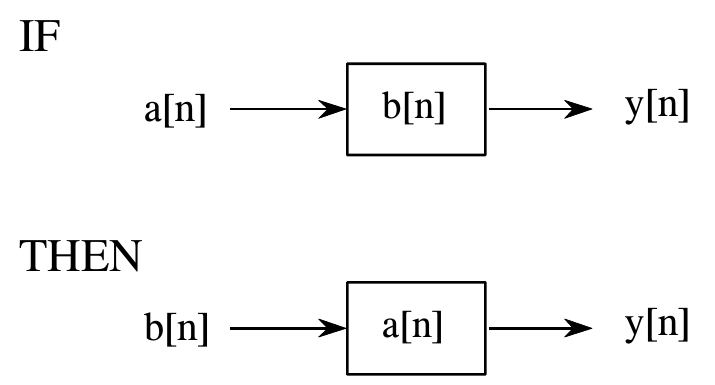
\includegraphics[width=0.596\linewidth,height=0.8\textheight,keepaspectratio]{assets/ch07/fig7-08.png}
\caption*{\textbf{图 7-8　系统理论中的交换律。}
卷积的交换律使得系统的输入信号和冲激响应可以互换，而输出不变。这很有意思，但通常没有物理意义。（方框里出现的信号，比如本图中的
b{[}n{]} 和 a{[}n{]}，表示系统的冲激响应。） （IF = 如果，THEN =
那么。）}
\end{figure}

\subsection{结合律}

三个或更多信号能卷积吗？答案是能，结合律(associative
property)说明了怎么做：先把其中两个信号卷积，得到一个中间信号，再把这个中间信号与第三个信号卷积。结合律保证卷积的先后顺序无关紧要。写成公式：

\textbf{公式 7-7}　卷积的结合律，描述三个或更多信号怎样卷积。

\[\big(a[n] * b[n]\big) * c[n] = a[n] * \big(b[n] * c[n]\big)\]

结合律在系统理论中用来描述级联(cascade)系统的行为。如图 7-9
所示，如果一个系统的输出用作下一个系统的输入，就说这两个或更多系统是级联的。根据结合律，级联中各系统的顺序可以重新排列，而整个级联的总响应不变。进一步说，任意多个级联的系统都可以用单个系统代替。这个替代系统的冲激响应，等于所有原系统冲激响应的卷积。

\begin{figure}[htbp]
\centering
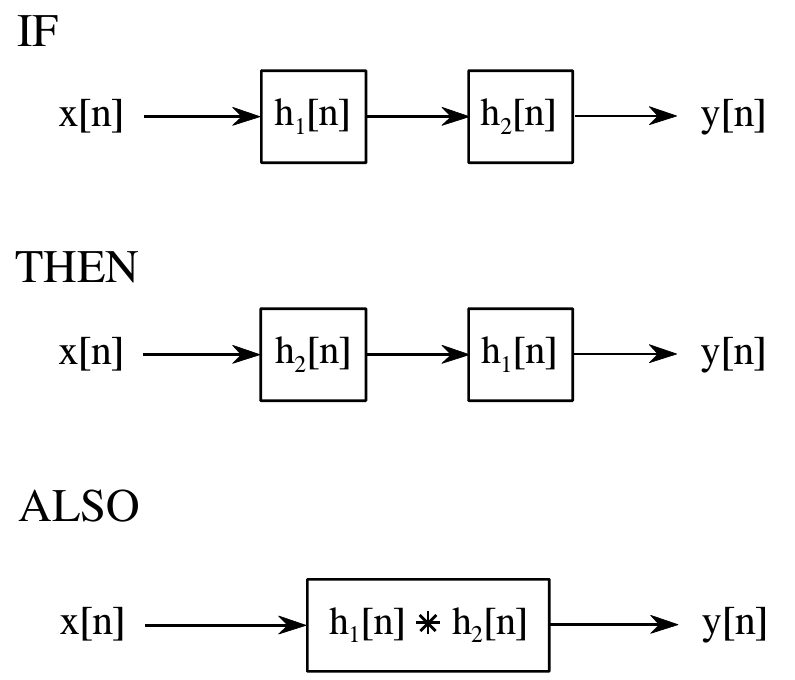
\includegraphics[width=0.662\linewidth,height=0.8\textheight,keepaspectratio]{assets/ch07/fig7-09.png}
\caption*{\textbf{图 7-9　系统理论中的结合律。}
结合律给出了级联线性系统的两个重要特点。第一，级联中各系统的顺序可以重新排列，而整个级联的作用不变。第二，级联中的两个或更多系统可以用单个系统代替，替代系统的冲激响应等于被替换各级冲激响应的卷积。
（IF = 如果，THEN = 那么，ALSO = 并且；最下一行方框里的 \dspsym{∗}
是卷积。）}
\end{figure}

\subsection{分配律}

分配律(distributive property)写成公式是：

\textbf{公式 7-8}　卷积的分配律，描述怎样分析并联系统。

\[a[n] * b[n] + a[n] * c[n] = a[n] * \big(b[n] + c[n]\big)\]

分配律描述了输出相加的并联(parallel)系统怎样工作。如图 7-10
所示，两个或更多系统可以共用同一个输入 x{[}n{]}，再把它们的输出相加得到
y{[}n{]}。分配律允许用单个系统代替这种组合，它的冲激响应等于各原系统冲激响应之和。

\begin{figure}[htbp]
\centering
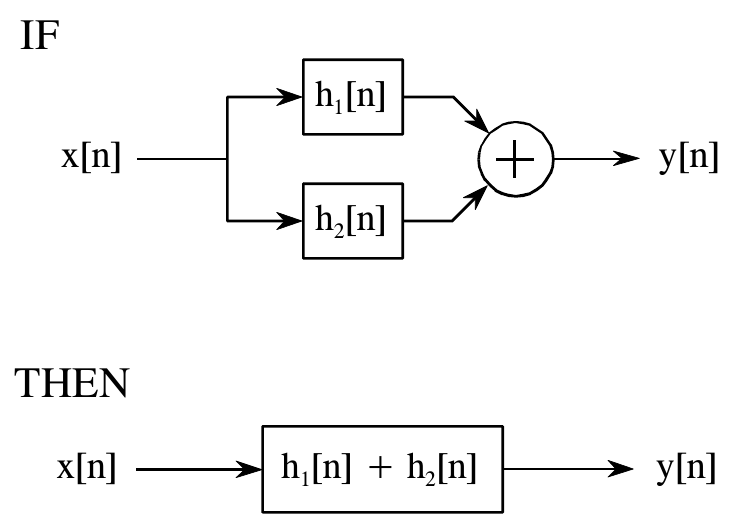
\includegraphics[width=0.621\linewidth,height=0.8\textheight,keepaspectratio]{assets/ch07/fig7-10.png}
\caption*{\textbf{图 7-10　系统理论中的分配律。}
分配律表明，输出相加的并联系统可以用单个系统代替。替代系统的冲激响应等于所有原系统冲激响应之和。
（IF = 如果，THEN = 那么；圆圈里的 + 表示相加。）}
\end{figure}

\subsection{输入与输出之间的传递}

这不算一条正式的数学性质，而是对信号处理中一种常见情形的思考方式。如图
7-11 所示，设想一个线性系统接收输入信号 x{[}n{]}，产生输出信号
y{[}n{]}。现在假设输入信号以某种线性方式改变了，得到一个新的输入信号，记作
x′{[}n{]}。这会产生一个新的输出信号
y′{[}n{]}。问题是：输入信号的改变和输出信号的改变之间有什么关系？答案是：输出信号以与输入信号完全相同的线性方式改变。例如，如果输入信号放大两倍，输出信号也放大两倍。如果对输入信号求导，输出信号也被求导。如果输入以某种方式被滤波，输出也会以完全相同的方式被滤波。用结合律很容易证明这一点。

\begin{figure}[htbp]
\centering
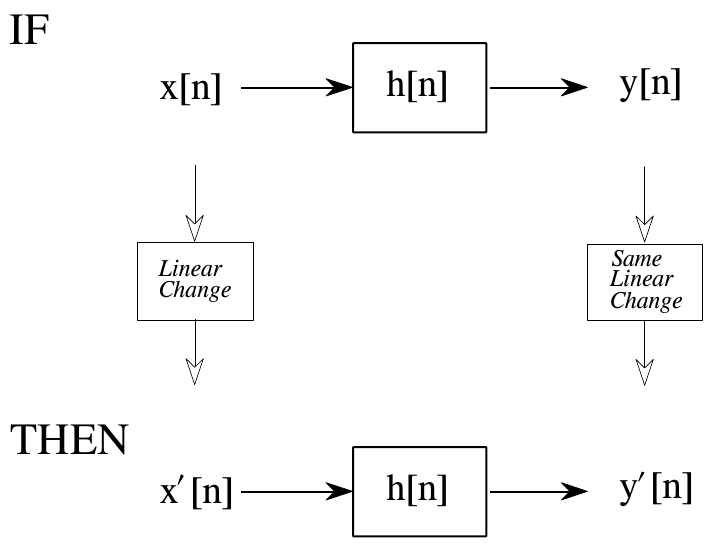
\includegraphics[width=0.596\linewidth,height=0.8\textheight,keepaspectratio]{assets/ch07/fig7-11.png}
\caption*{\textbf{图 7-11　输入与输出之间的传递(transference)。}
这是对信号处理中一种常见情形的思考方式：对输入信号做的线性改变，会导致输出信号发生同样的线性改变。
（IF = 如果，THEN = 那么，Linear Change = 线性改变，Same Linear Change =
同样的线性改变。原书图注把 Transference 误拼成 Tranference。）}
\end{figure}

\subsection{中心极限定理}

中心极限定理(Central Limit
Theorem)是概率论中的一个重要工具，因为它从数学上解释了为什么高斯概率分布在自然界中如此常见。例如：电子电路中热噪声的幅度服从高斯分布；激光束横截面上的光强是高斯分布；就连飞镖盘靶心周围的扎孔分布也是高斯分布。中心极限定理最简单的表述是：当被观测的变量是许多随机过程之和时，就会得到高斯分布。即使各个组成过程本身不是高斯分布，它们的和也是。

中心极限定理对卷积有一个有趣的推论：如果把一个脉冲状的信号与自身卷积很多次，就会得到一个高斯曲线。图
7-12 是一个例子。(a)
中的信号是一个不规则的脉冲，特意选得一点也不像高斯曲线。(b)
是这个信号与自身卷积一次的结果。(c)
是这个信号与自身卷积三次的结果。只卷积了三次，波形就已经很像高斯曲线了。用数学行话说，这个过程收敛到高斯曲线的速度非常快。所得高斯曲线的宽度（即公式
2-7 或 2-8 中的 σ），等于原脉冲的宽度（用公式 2-7 中的 σ
表示）乘以卷积次数的平方根。

\begin{figure}[htbp]
\centering
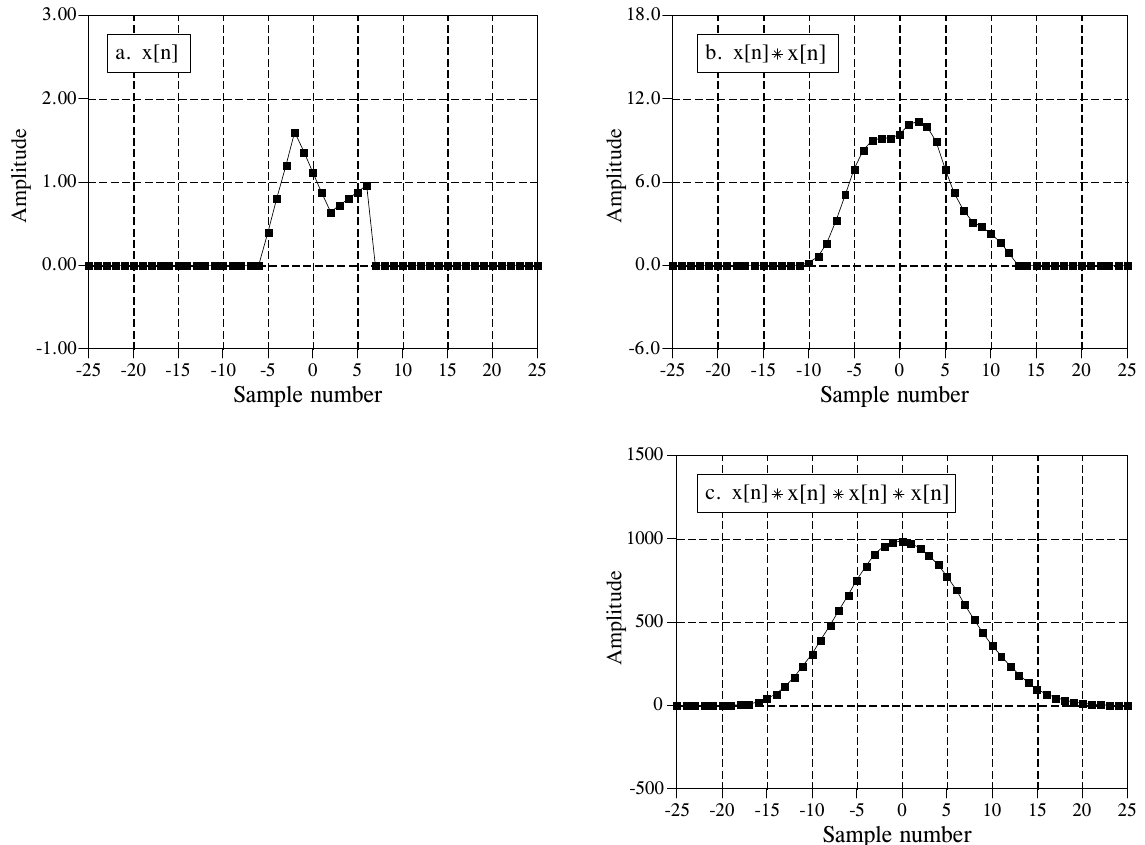
\includegraphics[width=0.954\linewidth,height=0.8\textheight,keepaspectratio]{assets/ch07/fig7-12.png}
\caption*{\textbf{图 7-12　脉冲波形与自身卷积的例子。}
中心极限定理表明，任意形状的脉冲与自身卷积很多次后会得到高斯波形。(a)
是一个示例脉冲。(b) 中脉冲与自身卷积一次，已开始显得平滑规整。(c)
中脉冲与自身卷积三次，已非常接近高斯曲线。 （a. x{[}n{]}；b. x{[}n{]}
\dspsym{∗} x{[}n{]}；c.~x{[}n{]} \dspsym{∗} x{[}n{]} \dspsym{∗} x{[}n{]}
\dspsym{∗} x{[}n{]}。Amplitude = 幅度，Sample number = 采样序号。）}
\end{figure}

\section{相关}

相关(correlation)的概念最好用一个例子来说明。图 7-13
画出了雷达系统的关键组成部分。一副特别设计的天线朝选定的方向发出一小段无线电波能量。如果传播中的电波碰到物体，比如图中的直升机，就会有一小部分能量被反射回来，射向位于发射机附近的无线电接收机。发射的脉冲是我们选定的某种特定形状，比如本例中的三角形。接收到的信号由两部分组成：(1)
发射脉冲的一个平移并缩放过的版本；(2)
随机噪声，来自干扰电波、电子器件中的热噪声等。由于无线电信号以已知的速度（光速）传播，发射脉冲和接收脉冲之间的平移量，直接反映了被探测物体的距离。问题是：给定一个已知形状的信号，怎样才能最好地判断它在另一个信号中出现在哪里（或者有没有出现）？相关就是答案。

\begin{figure}[htbp]
\centering
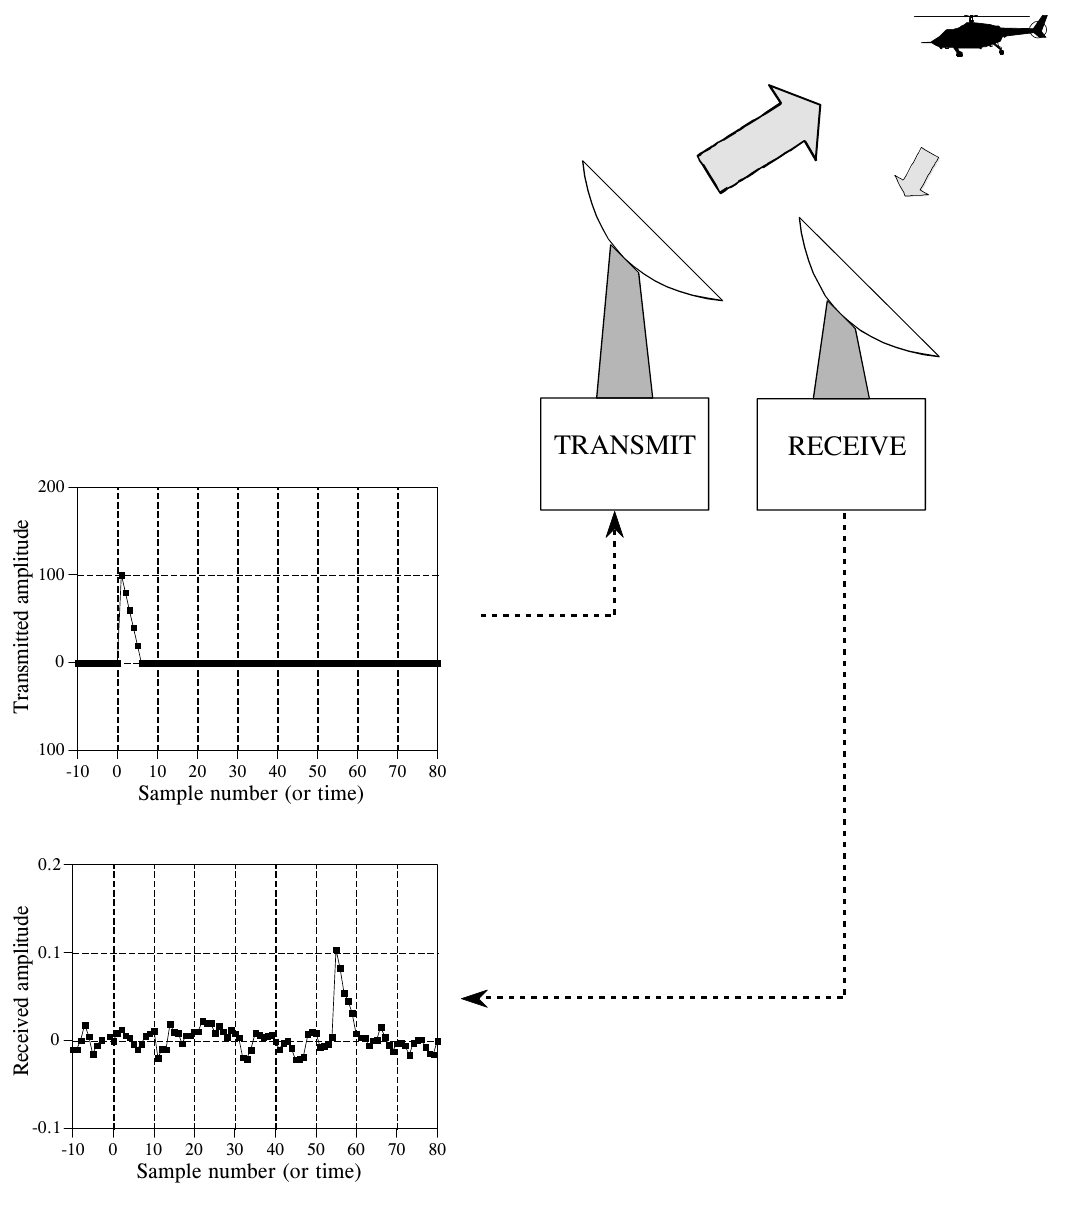
\includegraphics[width=0.887\linewidth,height=0.8\textheight,keepaspectratio]{assets/ch07/fig7-13.png}
\caption*{\textbf{图 7-13　雷达系统的关键组成部分。}
和其他回声定位系统一样，雷达发出一个短能量脉冲，被所考察的物体反射回来。这使得接收到的波形是发射波形的平移版本加上随机噪声。在含噪信号中检测已知波形，是回声定位的根本问题。这个问题的答案就是相关。
（TRANSMIT = 发射，RECEIVE = 接收；Transmitted amplitude =
发射幅度，Received amplitude = 接收幅度，Sample number (or time) =
采样序号（或时间）。发射幅度纵轴最下面的刻度在原书中显示为 100，应为
−100。）}
\end{figure}

相关是一种与卷积非常相似的数学运算。和卷积一样，相关用两个信号产生第三个信号。这第三个信号叫做两个输入信号的互相关(cross-correlation)。如果一个信号与它自身做相关，得到的信号则叫自相关(autocorrelation)。上一章用卷积机说明了卷积是怎样执行的。图
7-14 是一个类似的相关机(correlation machine)示意图。接收信号 x{[}n{]}
和互相关信号 y{[}n{]} 固定在纸面上。我们要寻找的波形
t{[}n{]}，通常叫做目标信号(target signal)，装在相关机里面。计算 y{[}n{]}
中的每个采样时，把相关机向左或向右移动，直到它指向正在计算的那个采样。然后，接收信号中被指到的那些采样落进相关机，与目标信号中对应的点相乘。这些乘积之和送入互相关信号中相应的采样。

\begin{figure}[htbp]
\centering
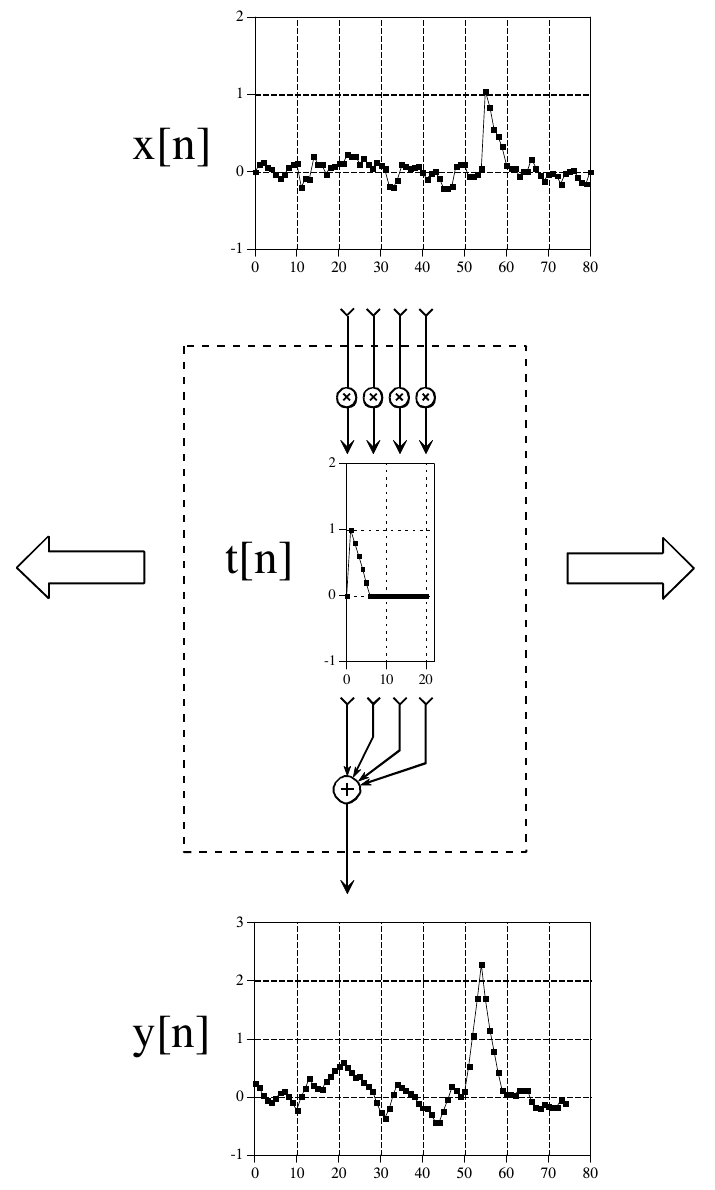
\includegraphics[width=0.596\linewidth,height=0.8\textheight,keepaspectratio]{assets/ch07/fig7-14.png}
\caption*{\textbf{图 7-14　相关机。}
这是一张展示两个信号的互相关怎样计算的流程图。本例中，y{[}n{]} 是
x{[}n{]} 与 t{[}n{]} 的互相关。虚线框左右移动，使它的输出指向 y{[}n{]}
中正在计算的采样。x{[}n{]} 中被指到的采样与 t{[}n{]}
中对应的采样相乘，再把乘积相加。相关机与卷积机（图 6-8 和
6-9）完全相同，只是虚线框里的信号没有左右翻转。本图中，y{[}n{]} 只计算了
t{[}n{]} 完全浸没在 x{[}n{]} 中的那些采样。
（横轴为采样序号（或时间）。）}
\end{figure}

互相关信号中每个采样的幅度，衡量的是接收信号在该位置与目标信号有多相像。这意味着，接收信号里每出现一个目标信号，互相关信号中就会出现一个峰。换句话说，当目标信号与接收信号中相同的特征对齐时，互相关的值达到最大。

如果目标信号含有负值采样怎么办？什么都不变。设想相关机所处的位置恰好使目标信号与接收信号中相匹配的波形完全对齐。接收信号的采样落进相关机时，与目标信号中和它们相匹配的采样相乘。忽略噪声的话，正的采样与自身相乘，得到正数；同样，负的采样与自身相乘，也得到正数。即使目标信号完全是负的，互相关中的峰仍然是正的。

如果接收信号上有噪声，互相关信号上也会有噪声。随机噪声总会在一定程度上像你所选的任何目标信号，这是无法避免的事实。互相关信号上的噪声，衡量的正是这种相似程度。除了这种噪声，互相关信号中产生的峰是左右对称的，即使目标信号本身不对称也是如此。此外，峰的宽度是目标信号宽度的两倍。记住，互相关是在检测目标信号，而不是重建它。没有理由指望这个峰长得像目标信号。

相关是在随机噪声中检测已知波形的最优技术。也就是说，用相关得到的峰高出噪声的程度，比任何其他线性系统能做到的都高。（严格地说，它只对随机白噪声是最优的。）用相关来检测已知波形，常被称为匹配滤波(matched
filtering)。第 17 章会更多地讲到这一点。

相关机和卷积机完全相同，只有一点小区别。上一章讲过，卷积机里的信号是左右翻转的。这意味着序号
1、2、3、\dspsym{⋯}
从右往左排列。在相关机里不做这个翻转，采样按正常方向排列。

既然信号翻转是两种运算唯一的区别，就可以用和卷积相同的数学来表示相关。这需要预先把参与相关的两个信号之一翻转过来，以抵消卷积本身固有的左右翻转。例如，a{[}n{]}
和 b{[}n{]} 卷积得到 c{[}n{]} 时，公式写作
\(a[n] * b[n] = c[n]\)。相比之下，a{[}n{]} 和 b{[}n{]} 的互相关可以写作
\(a[n] * b[-n] = c[n]\)。也就是说，把 b{[}n{]}
左右翻转，是通过把下标取反实现的，即 b{[}−n{]}。

别让卷积和相关在数学上的相似性迷惑了你，它们代表截然不同的 DSP
过程。卷积是系统的输入信号、输出信号和冲激响应之间的关系；相关是在噪声背景中检测已知波形的一种方法。数学上的相似只是一个方便的巧合。

\section{速度}

写一个把一个信号与另一个信号卷积的程序很简单，只需要几行代码。执行这个程序可能就痛苦多了。问题在于算法需要大量的加法和乘法，导致执行时间很长。从上一章的程序可以看出，耗时的操作是把两个数相乘，再把结果加到一个累加器上。算法的其他部分，比如数组的索引，都非常快。乘加(multiply-accumulate)是
DSP 的一个基本构件，我们会在其他几个重要算法中一再看到它。事实上，DSP
计算机的速度常常就用完成一次乘加所需的时间来标定。

一个由 N 个采样组成的信号与一个由 M 个采样组成的信号卷积，必须执行 N×M
次乘加。这从上一章的程序就能看出。1990
年代中期的个人计算机，每次乘加大约需要一微秒（100 MHz
奔腾，使用单精度浮点数，见表 4-6）。因此，把一个 10,000 点的信号与一个
100 点的信号卷积大约需要一秒。处理一个一百万点的信号、配一个 3000
点的冲激响应，需要将近一小时。再早十年（12 MHz 的
80286），这个计算需要三天！

执行时间过长的问题通常用三种方法之一来解决。第一，信号尽量短，并且用整数而不用浮点数。如果你只需要运行几次卷积，这大概是执行时间与编程工作量之间最好的折中。第二，使用专为
DSP 设计的计算机。DSP
微处理器的乘加时间只有几十纳秒。如果你打算大量执行卷积，比如在设计商业产品时，就该走这条路。

第三种办法是使用更好的卷积算法。第 17 章会介绍一种非常精巧的算法，叫 FFT
卷积(FFT convolution)。FFT
卷积得到的结果与上一章介绍的卷积算法完全相同，但执行时间大大缩短。对于几千个采样的信号，FFT
卷积可以快几百倍。缺点是程序复杂。即使你熟悉这种技术，也要准备花几个小时才能让程序跑起来。

% !TEX root = ../main.tex
% 本文件由 build-tex.sh 从 08-DSP指南-第8章中译.md 生成，改内容请改 md 后重新生成

\chapter{离散傅里叶变换}\label{ch-08}

傅里叶分析(Fourier
analysis)是一族数学方法，它们的共同基础是把信号分解成正弦波(sinusoids)。离散傅里叶变换(discrete
Fourier transform，DFT)是这一族里用于数字化信号的那个成员。本章是讲实数
DFT(real DFT)的四章中的第一章。实数 DFT
是离散傅里叶变换的一个版本，它用实数表示输入和输出信号。复数 DFT(complex
DFT)是一种更高级的方法，要用到复数，第 31
章再讨论。本章介绍傅里叶分解的数学和算法，这是 DFT 的核心。

\section{傅里叶变换家族}

傅里叶分析得名于让·巴蒂斯特·约瑟夫·傅里叶(Jean Baptiste Joseph
Fourier，1768--1830)，一位法国数学家和物理学家。（Fourier 读作
for-ē-ā，首字母总是大写。）虽然有很多人为这个领域作出过贡献，但傅里叶受到推崇，是因为他的数学发现，以及他看出了这些方法的实际用处。傅里叶研究的是热的传播。1807
年，他向法兰西研究院(Institut de
France)提交了一篇论文，讲怎样用正弦波来表示温度分布。论文里有一个颇具争议的论断：任何连续的周期信号，都可以表示成一组适当选取的正弦波之和。审稿人中有历史上两位最著名的数学家：约瑟夫·路易·拉格朗日(Joseph
Louis Lagrange，1736--1813)和皮埃尔·西蒙·德·拉普拉斯(Pierre Simon de
Laplace，1749--1827)。

拉普拉斯和其他审稿人投票同意发表，拉格朗日却坚决反对。将近 50
年来，拉格朗日一直坚持说，这种方法不能用来表示带拐角的信号，也就是斜率不连续的信号，比如方波。法兰西研究院屈从于拉格朗日的威望，拒绝了傅里叶的论文。直到拉格朗日去世之后，这篇论文才终于发表，那已是大约
15
年以后了。幸运的是，傅里叶还有别的事情要忙：政治活动、随拿破仑远征埃及，以及在法国大革命之后设法躲过断头台（这可不是比喻！）。

到底谁对呢？可以说各对一半。拉格朗日断言正弦波之和不能构成带拐角的信号，这一点是对的。但是，你可以非常接近它，接近到两者之差的能量为零。在这个意义上，傅里叶是对的，尽管
18 世纪的科学对能量的概念知道得很少。这个现象现在叫吉布斯效应(Gibbs
Effect)，第 11 章会讨论。

图 8-1 演示了怎样把一个信号分解成正弦波和余弦波。图 (a)
是一个示例信号，长 16 个点，采样序号从 0 到 15。图 (b)
是这个信号的傅里叶分解：九个余弦波和九个正弦波，每个都有不同的频率和幅度。虽然一眼看不出来，但这
18 个正弦波加起来正好得到 (a)
中的波形。要注意，拉格朗日的反对意见只适用于连续信号。对离散信号来说，这种分解在数学上是精确的。(a)
中的信号和 (b) 中各信号之和没有任何区别，就像 7 和 3+4 没有区别一样。

\begin{figure}[htbp]
\centering
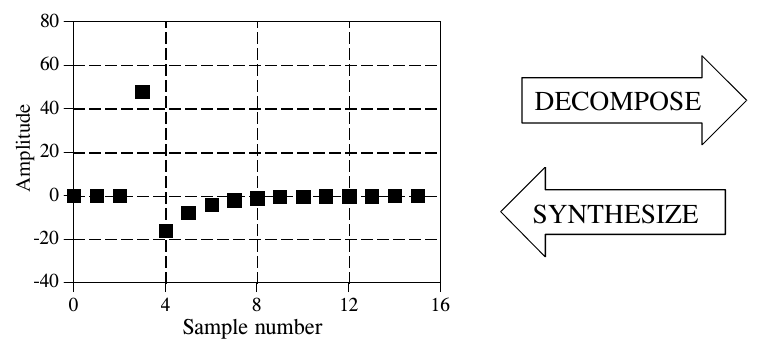
\includegraphics[width=0.633\linewidth,height=0.8\textheight,keepaspectratio]{assets/ch08/fig8-01a.png}
\caption*{\textbf{图 8-1a　一个 16 点的示例信号。}（对应的分解见下一张图 8-1b。）
（Amplitude = 幅度，Sample number = 采样序号，DECOMPOSE =
分解，SYNTHESIZE = 合成。）}
\end{figure}

\begin{figure}[htbp]
\centering
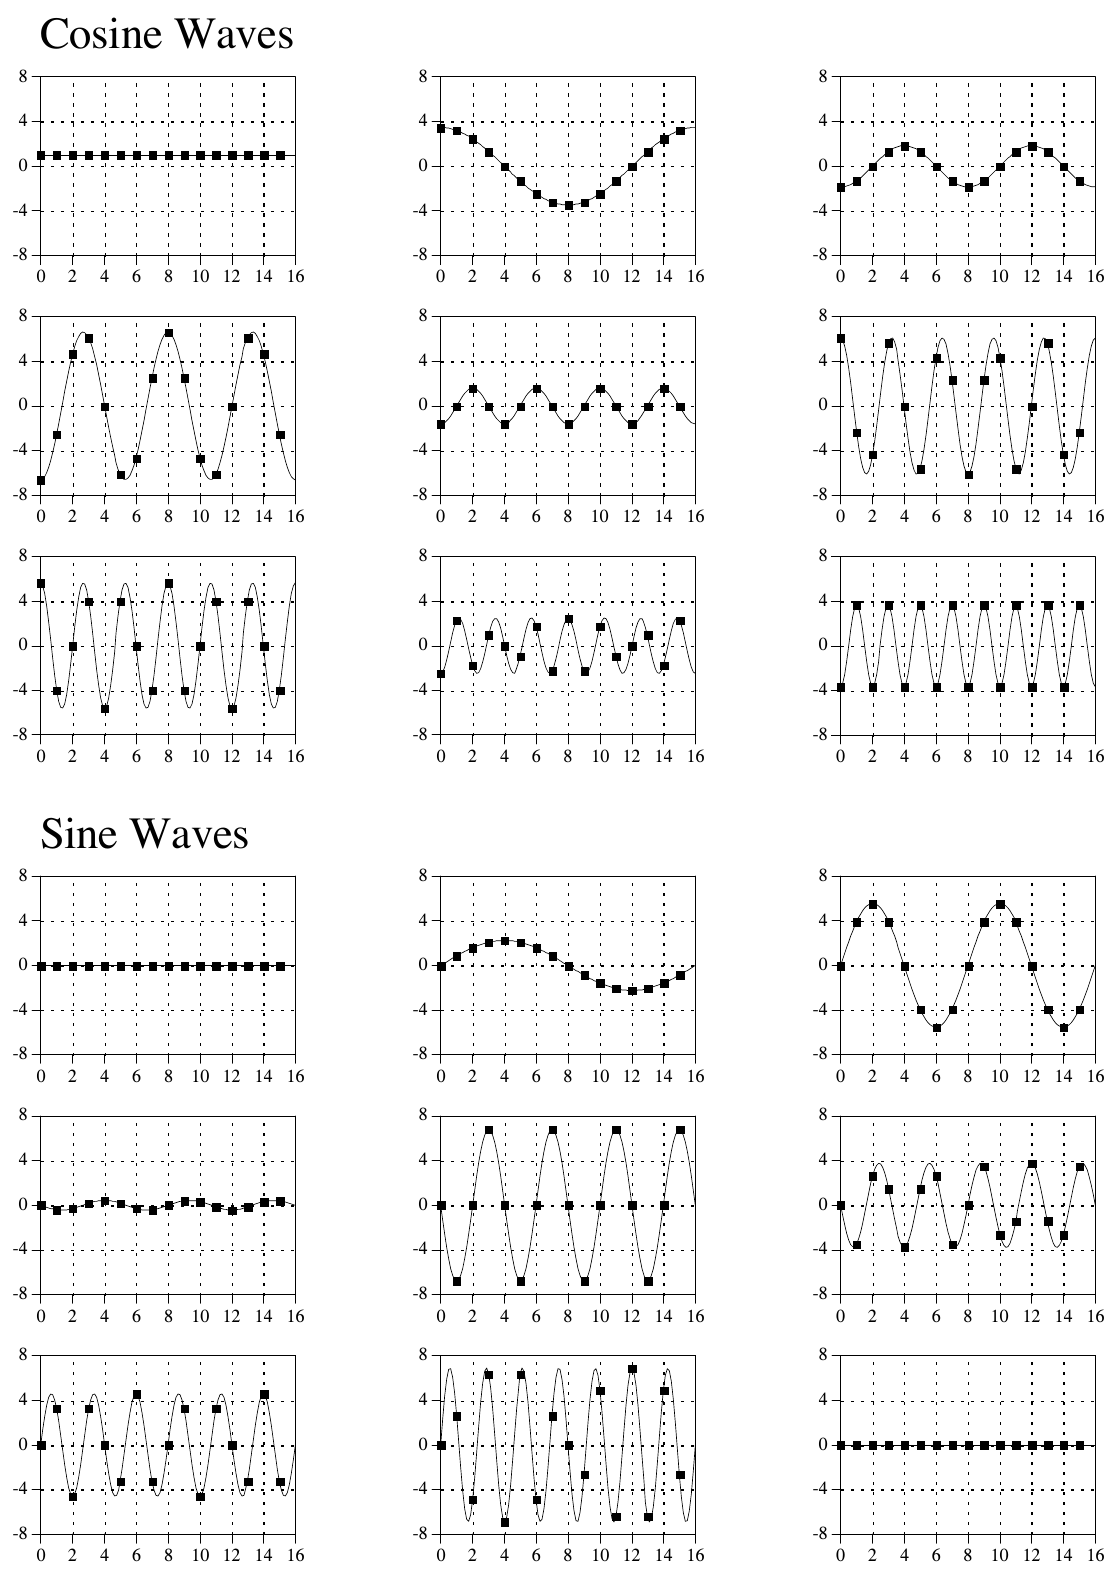
\includegraphics[width=0.925\linewidth,height=0.8\textheight,keepaspectratio]{assets/ch08/fig8-01b.png}
\caption*{\textbf{图 8-1b　傅里叶分解的例子。} 一个 16 点的信号（图 8-1a）被分解成
9 个余弦波和 9
个正弦波。每个正弦波的频率是固定的，只有幅度会随被分解的波形而变。
（Cosine Waves = 余弦波，Sine Waves =
正弦波。每组九幅图按从左到右、从上到下的顺序，频率依次为 0～8，即在 16
个点里走完 0～8 个周期。）}
\end{figure}

为什么用正弦波，而不用比如方波或三角波？记住，分解一个信号的方法有无穷多种。分解的目的，是得到一些比原信号更容易处理的东西。例如，冲激分解让我们可以一次考察信号的一个点，由此得到了卷积这一强大的方法。分量正弦波和余弦波比原信号简单，是因为它们具有一个原信号没有的性质：正弦保真性(sinusoidal
fidelity)。第 5
章讲过，正弦波输入一个系统，保证得到的输出也是正弦波。只有信号的幅度和相位可以改变，频率和波形必须保持不变。正弦波是唯一具有这一有用性质的波形。方波或三角波分解虽然也做得到，但一般没有理由说它们有用。

傅里叶变换(Fourier
transform)这个总称可以分成四类，对应可能遇到的四种基本信号类型。一个信号可以是连续的或离散的，也可以是周期的或非周期的。这两个特征组合起来就得到四类，下面分别说明，并画在图
8-2 中。

\textbf{非周期---连续(Aperiodic-Continuous)}
例如衰减指数函数和高斯曲线。这类信号向正负无穷两个方向延伸，不按周期模式重复。用于这类信号的傅里叶变换就叫傅里叶变换(Fourier
Transform)。

\textbf{周期---连续(Periodic-Continuous)}
例子有：正弦波、方波，以及任何从负无穷到正无穷按固定模式重复的波形。这一版本的傅里叶变换叫傅里叶级数(Fourier
Series)。

\textbf{非周期---离散(Aperiodic-Discrete)}
这类信号只在正负无穷之间的离散点上有定义，并且不按周期重复。这类傅里叶变换叫离散时间傅里叶变换(Discrete
Time Fourier Transform，DTFT)。

\textbf{周期---离散(Periodic-Discrete)}
这是从负无穷到正无穷周期重复的离散信号。这一类傅里叶变换有时叫离散傅里叶级数(Discrete
Fourier Series)，但最常用的名字是离散傅里叶变换(Discrete Fourier
Transform)。

你可能会觉得，这四种傅里叶变换的名字既混乱又没条理。你说得对，这些名字是在
200
年里相当随意地演变出来的。你没有别的办法，只能把它们记住，然后继续往下学。

这四类信号都向正负无穷延伸。等一等，你会说！如果计算机里只存了有限个采样，比如一个
1024
点的信号，怎么办？难道没有一种适用于有限长信号的傅里叶变换吗？没有。正弦波和余弦波的定义就是从负无穷延伸到正无穷。你没法用一组无限长的信号去合成一个有限长的东西。绕过这个难题的办法，是让有限长的数据看起来像一个无限长的信号。做法是想象在实际数据点的左右两边还有无穷多个采样。如果这些''想象出来''的采样全为零，信号看起来就是离散、非周期的，适用离散时间傅里叶变换。另一种做法是让想象出来的采样都是这
1024 个实际点的复制。这时信号看起来是离散、周期的，周期为 1024
个采样，于是就要用离散傅里叶变换。

结果是，合成一个非周期信号需要无穷多个正弦波。这使得离散时间傅里叶变换不可能用计算机算法算出来。排除之后，DSP
中唯一能用的傅里叶变换就是
DFT。换句话说，数字计算机只能处理离散、有限长的信息。当你钻研理论问题、对付习题、琢磨数学谜题时，可能会用到傅里叶变换家族的前三个成员。当你坐到计算机前，你只会用
DFT。后面的章节会简要介绍其他几种傅里叶变换。眼下，请集中精力理解离散傅里叶变换。

\begin{figure}[htbp]
\centering
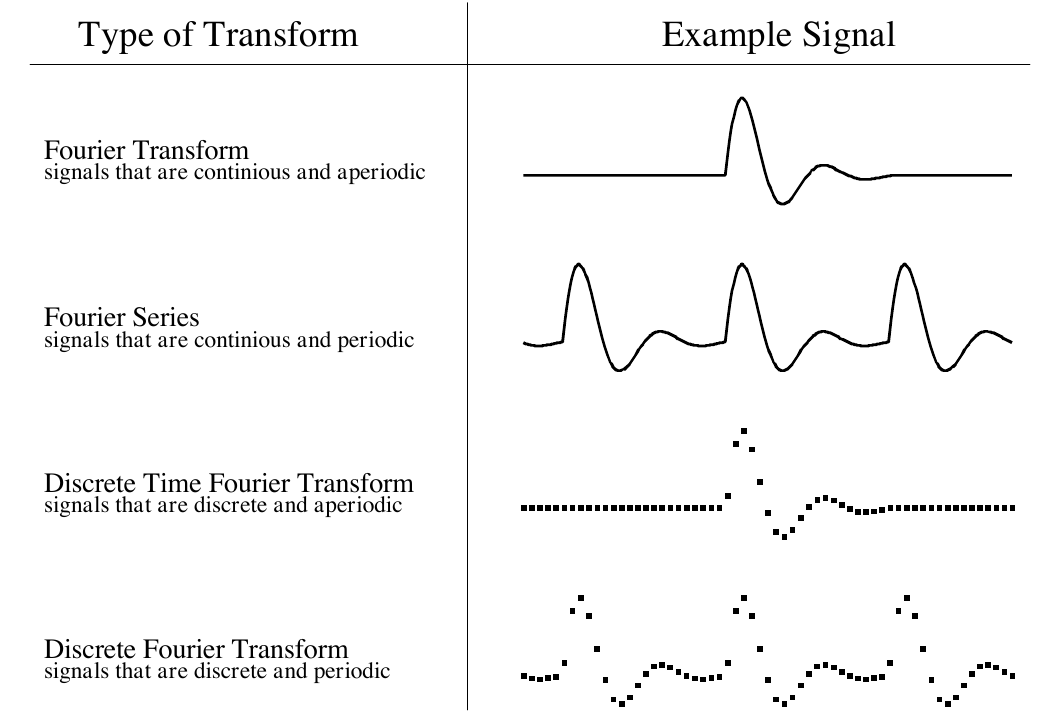
\includegraphics[width=0.875\linewidth,height=0.8\textheight,keepaspectratio]{assets/ch08/fig8-02.png}
\caption*{\textbf{图 8-2　四种傅里叶变换的示意图。}
信号可以是连续的或离散的，也可以是周期的或非周期的。两两组合得到四种可能，每种都有自己版本的傅里叶变换。这些名字没什么条理，直接记住就好。
（Type of Transform = 变换类型，Example Signal = 示例信号；Fourier
Transform：signals that are continuous and aperiodic =
傅里叶变换：连续且非周期的信号；Fourier Series：continuous and periodic
= 傅里叶级数：连续且周期；Discrete Time Fourier Transform：discrete and
aperiodic = 离散时间傅里叶变换：离散且非周期；Discrete Fourier
Transform：discrete and periodic = 离散傅里叶变换：离散且周期。图中
continuous 原书误拼为 continious。）}
\end{figure}

回头看图 8-1 中的 DFT 分解示例。表面上看，这是一个 16 点信号被分解成 18
个正弦波，每个正弦波各有 16 个点。用更正式的说法，(a) 中的 16
点信号必须看作一个无限长周期信号的一个周期。同样，(b) 中的 18
个正弦波，每个都代表一个无限长正弦波中的一段 16 点。把这看作''用 16
点的正弦波合成一个 16
点信号''，还是''用无限长的正弦波合成一个无限长的周期信号''，这真的有关系吗？答案是：通常没关系，但有时有关系。后面的章节会遇到一些
DFT
的性质，如果把信号看作有限长，它们会显得莫名其妙；一旦考虑到周期性，就一目了然了。要理解的关键点是：引入这种周期性，是为了能使用一个数学工具，即
DFT。就信号从哪里来、怎样采集而言，这种周期性通常没有任何意义。

四种傅里叶变换各自都可以再分成实数版本和复数版本。实数版本最简单，合成与分解只用普通的数和代数。例如，图
8-1 就是一个实数 DFT
的例子。四种傅里叶变换的复数版本要复杂得多，需要用到复数。复数是像
\(3 + 4j\) 这样的数，其中 \(j\) 等于 \(\sqrt{-1}\)（电气工程师用变量
j，数学家用变量 i）。复数数学很快就会让人吃不消，即使是专门做 DSP
的人也一样。事实上，本书的一个主要目标就是不用复数数学来讲解 DSP
的基础，让更多的科学家和工程师能看懂。复数傅里叶变换是那些专攻
DSP、并且愿意在数学沼泽里没到脖子的人的领地。如果你有这个兴趣，第 30～33
章会带你去那里。

变换(transform)这个数学术语在数字信号处理中用得非常多，比如：傅里叶变换、拉普拉斯变换(Laplace
transform)、Z 变换(Z transform)、希尔伯特变换(Hilbert
transform)、离散余弦变换(Discrete Cosine
transform)等等。变换到底是什么？要回答这个问题，先回想一下函数是什么。函数是把一个值变成另一个值的算法或过程。例如，\(y = 2x + 1\)
就是一个函数。你给 x 选一个值，代进方程，就会得到一个 y
值。函数也可以把几个值变成一个值，例如 \(y = 2a + 3b + 4c\)，它把
a、b、c 变成 y。

变换是函数的直接推广，它允许输入和输出都有多个值。假设你有一个由 100
个采样组成的信号。如果你设计出某个方程、算法或过程，能把这 100
个采样变成另外 100
个采样，你就有了一个变换。如果你觉得它够有用，你完全有权利把自己的姓冠在它前面，向同事们宣扬它的好处。（如果你是一位杰出的
18
世纪法国数学家，这招效果最好。）变换不限定数据的类型或数量。例如，输入可以是
100 个离散采样，输出可以是 200
个离散采样。同样，输入可以是连续信号，输出也是连续信号。混合的也行：离散输入、连续输出，或者反过来。简单地说，变换就是把一块数据变成另一块数据的任何固定过程。我们来看看这怎样用到眼下的主题：离散傅里叶变换。

\section{实数 DFT 的记号与格式}

如图 8-3 所示，离散傅里叶变换把一个 N 点的输入信号变成两个 N/2+1
点的输出信号。输入信号包含被分解的信号，两个输出信号包含各分量正弦波和余弦波的幅度（按一种稍后讨论的方式做了缩放）。输入信号被称为处在时域(time
domain)。这是因为进入 DFT
的信号最常见的是按固定时间间隔采集的采样。当然，任何采样数据都可以送进
DFT，不管它是怎样采集的。在傅里叶分析中看到''时域''这个词，它可能确实指随时间采集的采样，也可能只是泛指任何正在被分解的离散信号。频域(frequency
domain)这个词用来描述正弦波和余弦波的幅度（包括我们答应要解释的那种特殊缩放）。

\begin{figure}[htbp]
\centering
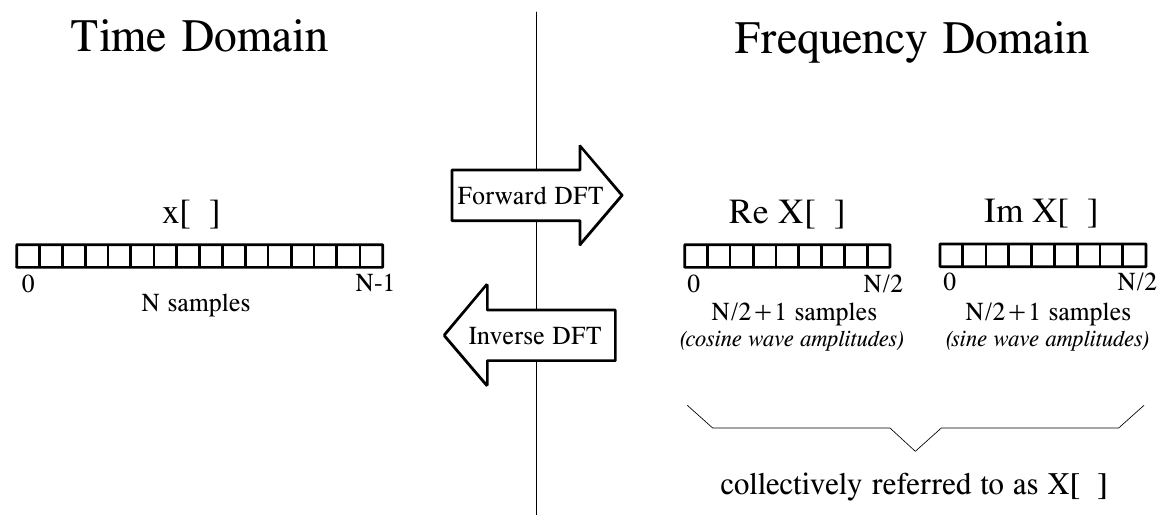
\includegraphics[width=0.975\linewidth,height=0.8\textheight,keepaspectratio]{assets/ch08/fig8-03.png}
\caption*{\textbf{图 8-3　DFT 的术语。} 在时域中，x{[} {]} 由 N 个点组成，序号从 0
到 N−1。在频域中，DFT 产生两个信号：实部(real part)，记作 Re X{[}
{]}；虚部(imaginary part)，记作 Im X{[} {]}。这两个频域信号各长 N/2+1
点，序号从 0 到 N/2。正向 DFT(Forward DFT)把时域变换到频域，逆
DFT(Inverse DFT)把频域变换回时域。（注意：本图描述的是实数 DFT。第 31
章讨论的复数 DFT 是把 N 个复数点变成另一组 N 个复数点。） （Time Domain
= 时域，Frequency Domain = 频域，N samples = N 个采样，N/2+1 samples =
N/2+1 个采样，cosine wave amplitudes = 余弦波幅度，sine wave amplitudes
= 正弦波幅度，collectively referred to as X{[} {]} = 合起来称为 X{[}
{]}。）}
\end{figure}

频域包含的信息和时域完全一样，只是形式不同。知道其中一个域，就能算出另一个。已知时域信号，计算频域的过程叫分解(decomposition)、分析(analysis)、正向
DFT(forward DFT)，或者干脆叫
DFT。已知频域，计算时域的过程叫合成(synthesis)，或逆 DFT(inverse
DFT)。合成与分析都可以写成方程，也都可以写成计算机算法。

时域中的采样数通常用变量 N 表示。N 可以是任何正整数，但通常选 2
的幂，比如 128、256、512、1024
等。原因有两个。第一，数字存储用二进制寻址，2
的幂是很自然的信号长度。第二，计算 DFT
最高效的算法------快速傅里叶变换(Fast Fourier
Transform，FFT)------通常要求 N 是 2 的幂。N 一般在 32 到 4096
之间。多数情况下，采样序号从 0 到 N−1，而不是从 1 到 N。

标准的 DSP 记法用小写字母表示时域信号，比如 x{[} {]}、y{[} {]}、z{[}
{]}。对应的大写字母表示它们的频域，即 X{[} {]}、Y{[} {]}、Z{[}
{]}。举例来说，假设一个 N 点的时域信号存放在 x{[} {]}
中。这个信号的频域叫 X{[} {]}，由两部分组成，每部分是一个 N/2+1
个采样的数组。它们叫 X{[} {]} 的实部，记作 Re X{[} {]}；以及 X{[} {]}
的虚部，记作 Im X{[} {]}。Re X{[} {]} 中的值是余弦波的幅度，Im X{[} {]}
中的值是正弦波的幅度（暂时不管缩放因子）。就像时域从 x{[}0{]} 到
x{[}N−1{]}，频域信号从 Re X{[}0{]} 到 Re X{[}N/2{]}、从 Im X{[}0{]} 到
Im X{[}N/2{]}。仔细研究这些记法，它们对理解 DSP
中的公式至关重要。可惜有些计算机语言不区分大小写，变量名只好由每个程序员自己定。本书的程序用数组
XX{[} {]} 存放时域信号，用数组 REX{[} {]} 和 IMX{[} {]} 存放频域信号。

实部和虚部这两个名字来自复数 DFT，在那里用来区分实数和虚数。实数 DFT
用不着这么复杂的东西。在学到第 31
章之前，只要把''实部''理解成余弦波的幅度、``虚部''理解成正弦波的幅度就行。别被这两个有暗示性的名字误导，这里用到的全是普通的数。

同样，也别被频域信号的长度误导。DSP 文献里常常看到这样的说法：``DFT 把 N
点的时域信号变成 N 点的频域信号。''这指的是复数
DFT，其中每个''点''都是一个复数（由实部和虚部组成）。现在先专心学实数
DFT，难的数学很快就会来。

\section{频域的自变量}

图 8-4 是一个 N = 128 的 DFT 示例。时域信号存放在数组 x{[}0{]} 到
x{[}127{]} 中。频域信号存放在两个数组 Re X{[}0{]} 到 Re X{[}64{]} 和 Im
X{[}0{]} 到 Im X{[}64{]} 中。注意，时域的 128 个点对应每个频域信号的 65
个点，频率序号从 0 到 64。也就是说，时域的 N 个点对应频域的 N/2+1
个点（不是 N/2 个点）。忘掉这个多出来的点，是 DFT 程序中的常见错误。

\begin{figure}[htbp]
\centering
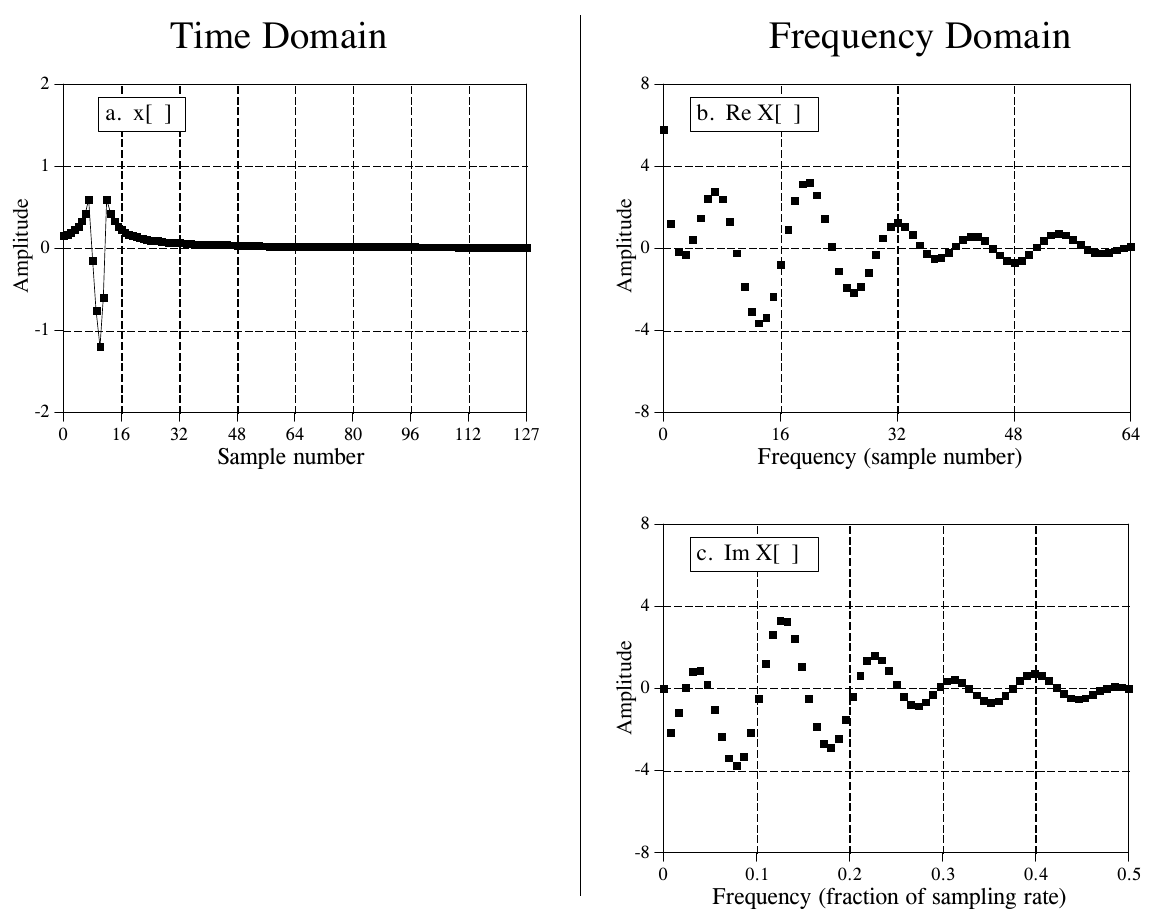
\includegraphics[width=0.958\linewidth,height=0.8\textheight,keepaspectratio]{assets/ch08/fig8-04.png}
\caption*{\textbf{图 8-4　DFT 的例子。} DFT 把时域信号 x{[} {]} 变换成频域信号 Re
X{[} {]} 和 Im X{[} {]}。频域的横轴可以用三种方式之一来标注：(1)
用数组下标，从 0 到 N/2；(2) 用采样频率的分数，从 0 到 0.5；(3)
用自然频率，从 0 到 π。本例中 (b) 用的是第一种方式，(c)
用的是第二种方式。 （Time Domain = 时域，Frequency Domain =
频域，Amplitude = 幅度，Sample number = 采样序号，Frequency (sample
number) = 频率（采样序号），Frequency (fraction of sampling rate) =
频率（采样率的分数）。译注：图注说''三种方式''，正文讲的是四种，第四种是用具体的模拟频率（赫兹）标注，图注没有列出。）}
\end{figure}

频域的横轴有四种不同的标注方式，在 DSP
中都很常见。第一种方式是把横轴标成 0 到 64，对应数组中的第 0 到第 N/2
个采样。用这种标注时，频域的下标是整数，例如 Re X{[}k{]} 和 Im
X{[}k{]}，其中 k 从 0 到 N/2，步长为
1。程序员喜欢这种方式，因为他们写代码就是这样，用一个下标访问数组元素。图
8-4b 用的就是这种记法。

第二种方式用在图 (c) 中，横轴标成采样率的分数。这意味着横轴上的值总是在
0 到 0.5
之间，因为离散数据只能包含从直流(DC)到采样率一半之间的频率。这种记法用的下标是
f，表示频率(frequency)。实部和虚部写成 Re X{[}f{]} 和 Im X{[}f{]}，其中
f 取 0 到 0.5 之间等间距的 N/2+1 个值。要从第一种记法 k 换成第二种记法
f，把横轴除以 N 即可，也就是
\(f = k/N\)。本书大多数图都用第二种方式，以强调离散信号只包含 0 到采样率
0.5 倍之间的频率。

第三种方式和第二种类似，只是横轴乘以 2π。这种标注用的下标是
ω，即小写的希腊字母 omega。在这种记法中，实部和虚部写成 Re X{[}ω{]} 和
Im X{[}ω{]}，其中 ω 取 0 到 π 之间等间距的 N/2+1 个值。参数 ω
叫自然频率(natural frequency)，单位是弧度(radians)。这是基于一个圆有 2π
弧度的想法。数学家喜欢这种方式，因为它让方程更短。例如，看看余弦波在前三种记法中各怎么写：用
k，\(c[n] = \cos(2\pi kn/N)\)；用 f，\(c[n] = \cos(2\pi fn)\)；用
ω，\(c[n] = \cos(\omega n)\)。

第四种方式是按具体应用中用到的模拟频率来标注横轴。例如，如果所研究的系统采样率是
10 kHz（即每秒 10,000 个采样），频域的图就从 0 画到 5
kHz。这种方式的优点是用真实世界的含义来呈现频率数据。缺点是它绑定了一个特定的采样率，因此不适用于一般的
DSP 算法开发，比如数字滤波器设计。

这四种记法在 DSP
中都有人用，你需要习惯在它们之间转换，图和数学公式都包括在内。要判断用的是哪种记法，看自变量和它的取值范围。你应该会看到以下四种之一：k（或别的整数下标），从
0 到 N/2；f，从 0 到 0.5；ω，从 0 到
π；或者用赫兹表示的频率，从直流到实际采样率的一半。

\section{DFT 的基函数}

DFT 中用到的正弦波和余弦波通常叫 DFT 的基函数(basis
functions)。换句话说，DFT 的输出是一组表示幅度的数，基函数则是一组幅度为
1
的正弦波和余弦波。如果把每个幅度（频域）分配给相应的正弦或余弦波（基函数），得到的就是一组经过缩放的正弦波和余弦波，把它们加起来就构成时域信号。

DFT 的基函数由下面的公式生成：

\textbf{公式 8-1　DFT 基函数的公式。} 式中 \(c_k[i]\) 和 \(s_k[i]\)
分别是余弦波和正弦波，每个长 N 点，i 从 0 到 N−1。参数 k
决定波的频率。在 N 点 DFT 中，k 取 0 到 N/2 之间的值。

\[
c_k[i] = \cos(2\pi k i / N)
\]

\[
s_k[i] = \sin(2\pi k i / N)
\]

其中 \(c_k[\,]\) 是与 Re X{[}k{]} 中的幅度对应的余弦波，\(s_k[\,]\) 是与
Im X{[}k{]} 中的幅度对应的正弦波。例如，图 8-5 画出了 N = 32 点 DFT
所用的 17 个正弦波和 17
个余弦波中的一部分。由于这些正弦波要相加构成输入信号，它们必须和输入信号一样长。本例中，每个都有
32 个点，i 从 0 到 31。参数 k
决定每个正弦波的频率。具体来说，\(c_1[\,]\) 是在 N
个点里走完一个完整周期的余弦波，\(c_5[\,]\) 是在 N
个点里走完五个完整周期的余弦波，依此类推。这是理解基函数的一个重要概念：频率参数
k 等于在信号的 N 个点里完成的完整周期数。

\begin{figure}[htbp]
\centering
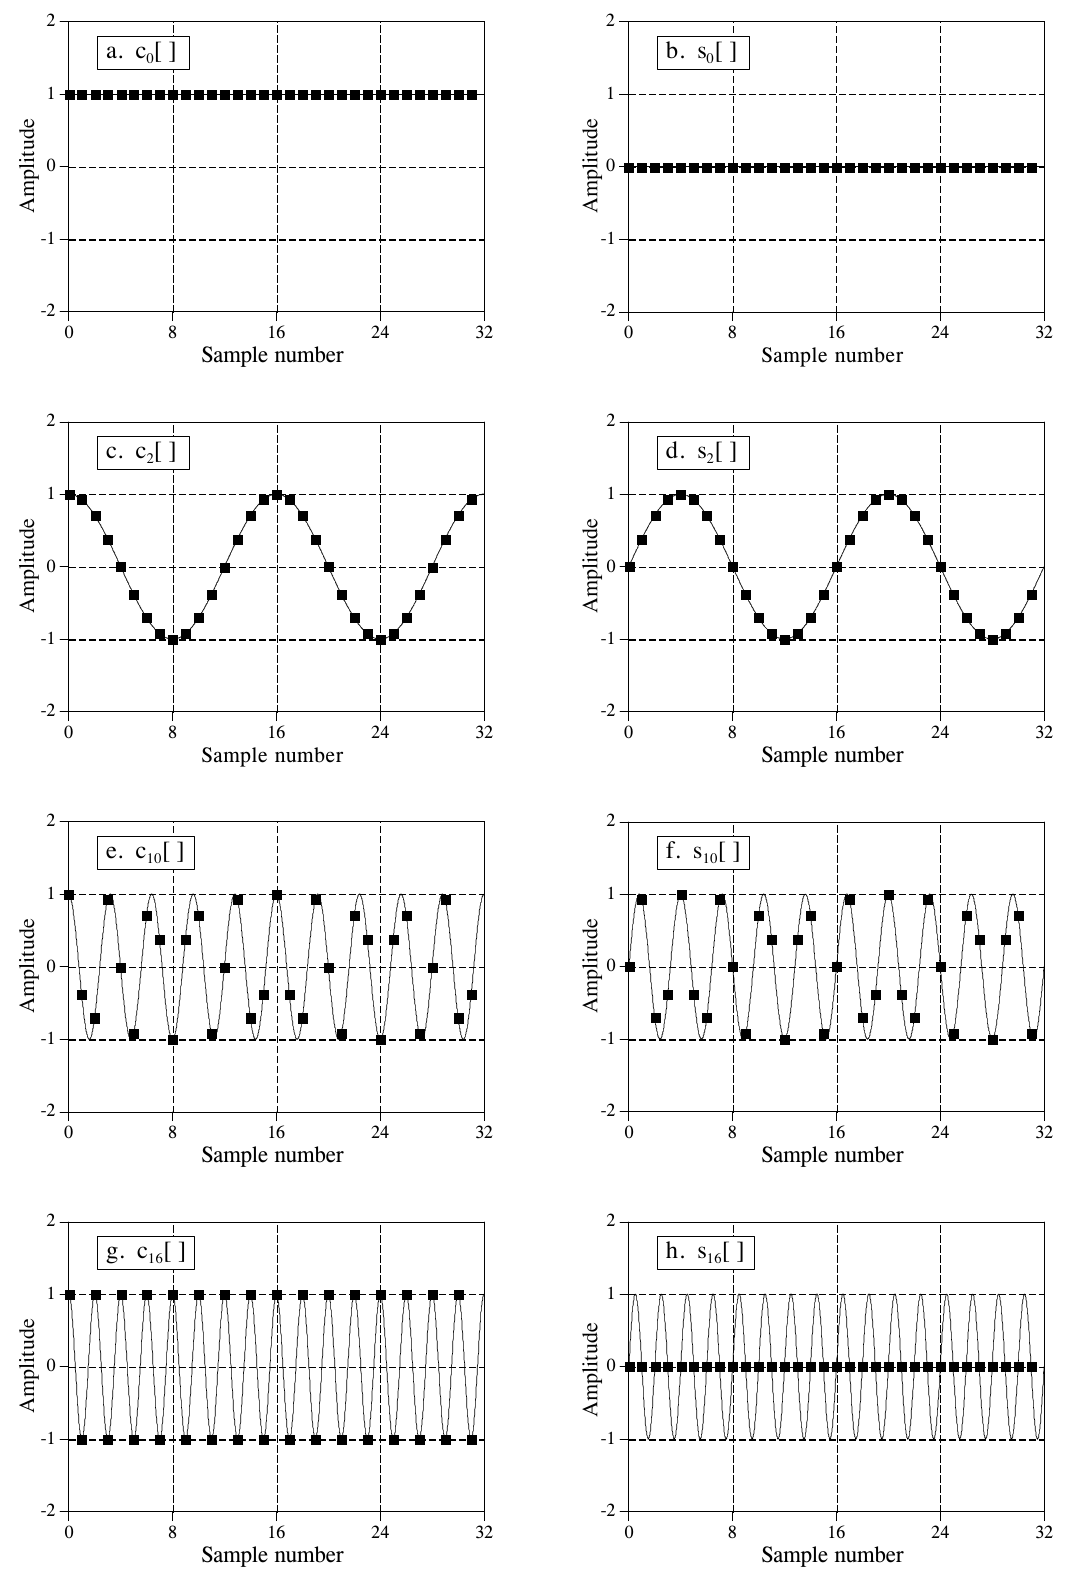
\includegraphics[width=0.892\linewidth,height=0.8\textheight,keepaspectratio]{assets/ch08/fig8-05.png}
\caption*{\textbf{图 8-5　DFT 的基函数。} 32 点 DFT 的基函数有 17 个离散余弦波和
17 个离散正弦波，本图画出其中 8
个。这些都是离散信号；图中的连续曲线只是为了帮助读者的眼睛跟上波形。
（Amplitude = 幅度，Sample number = 采样序号；a～h 分别为
\(c_0\)、\(s_0\)、\(c_2\)、\(s_2\)、\(c_{10}\)、\(s_{10}\)、\(c_{16}\)、\(s_{16}\)。）}
\end{figure}

我们来仔细看几个基函数。图 (a) 是余弦波
\(c_0[\,]\)。这是频率为零的余弦波，是恒为 1 的常数。这意味着 Re X{[}0{]}
存放的是时域信号所有点的平均值。在电子学里会说，Re X{[}0{]}
存放的是直流偏置(DC offset)。频率为零的正弦波 \(s_0[\,]\) 画在 (b)
中，是一个全为零的信号。由于它对合成的时域信号没有任何影响，Im X{[}0{]}
的值无关紧要，总是设为零。稍后还会细说。

图 (c) 和 (d) 是 \(c_2[\,]\) 和 \(s_2[\,]\)，即在 N
个点里完成两个周期的正弦波，分别对应 Re X{[}2{]} 和 Im
X{[}2{]}。同样，(e) 和 (f) 是 \(c_{10}[\,]\) 和 \(s_{10}[\,]\)，即在 N
个点里完成十个周期的正弦波，对应数组 Re X{[}10{]} 和 Im X{[}10{]}
中的幅度。问题是，(e) 和 (f)
中的采样看起来已经不像正弦波和余弦波了。如果图中没有那些连续曲线，你甚至很难看出波形的规律。这也许会让你有点不安，但不用担心。从数学角度看，这些采样确实构成离散的正弦波，即使你的眼睛跟不上它们的规律。

基函数中最高的频率画在 (g) 和 (h) 中。它们是 \(c_{N/2}[\,]\) 和
\(s_{N/2}[\,]\)，本例中就是 \(c_{16}[\,]\) 和
\(s_{16}[\,]\)。离散余弦波在 1 和 −1
之间交替取值，可以理解为在一个连续正弦波的波峰处采样。相反，离散正弦波全为零，这是在过零点处采样的结果。这使得
Im X{[}N/2{]} 和 Im X{[}0{]}
一样，总是等于零，对时域信号的合成没有影响。

这里有个谜题：如果进入 DFT 的是 N 个采样，出来的是 N+2
个采样，多出来的信息是从哪儿来的？答案是：有两个输出采样不含任何信息，这样其余
N 个采样才能完全独立。你可能已经猜到了，不含信息的两个点是 Im X{[}0{]}
和 Im X{[}N/2{]}，也就是总为零的那两个采样。

\section{合成：计算逆 DFT}

把到目前为止讲的内容合在一起，可以写出合成方程：

\textbf{公式 8-2　合成方程。} 式中 x{[}i{]} 是被合成的信号，下标 i 从 0
到 N−1。\(\mathrm{Re}\,\bar{X}[k]\) 和 \(\mathrm{Im}\,\bar{X}[k]\)
分别存放余弦波和正弦波的幅度，k 从 0 到 N/2。公式 8-3
给出把这个方程变成逆 DFT 所需的归一化。

\[
x[i] = \sum_{k=0}^{N/2} \mathrm{Re}\,\bar{X}[k]\cos(2\pi k i/N) + \sum_{k=0}^{N/2} \mathrm{Im}\,\bar{X}[k]\sin(2\pi k i/N)
\]

用文字说，任何 N 点信号 x{[}i{]}，都可以由 N/2+1 个余弦波和 N/2+1
个正弦波相加得到。余弦波和正弦波的幅度分别存放在数组
\(\mathrm{Re}\,\bar{X}[k]\) 和 \(\mathrm{Im}\,\bar{X}[k]\)
中。（译注：原书这里写成''分别存放在 Im X̄{[}k{]} 和 Re X̄{[}k{]}
中''，顺序颠倒了，余弦对应实部、正弦对应虚部。）合成方程把这些幅度乘以基函数，得到一组经过缩放的正弦波和余弦波。把这些缩放后的正弦波和余弦波相加，就得到时域信号
x{[}i{]}。

在公式 8-2 中，数组叫 \(\mathrm{Re}\,\bar{X}[k]\) 和
\(\mathrm{Im}\,\bar{X}[k]\)，而不是 Re X{[}k{]} 和 Im
X{[}k{]}。这是因为合成所需的幅度（在本节讨论中称为
\(\mathrm{Re}\,\bar{X}[k]\) 和
\(\mathrm{Im}\,\bar{X}[k]\)）和信号的频域（记作 Re X{[}k{]} 和 Im
X{[}k{]}）略有不同。这就是我们前面提到的缩放因子问题。虽然两者之间的转换只是一个简单的归一化，它却是计算机程序中的常见错误。要当心！写成公式，两者的转换是：

\textbf{公式 8-3　正弦波幅度与频域值之间的转换。} 式中
\(\mathrm{Re}\,\bar{X}[k]\) 和 \(\mathrm{Im}\,\bar{X}[k]\)
存放合成所需的余弦波和正弦波幅度，Re X{[}k{]} 和 Im X{[}k{]}
存放频域的实部和虚部。和往常一样，N 是时域信号的点数，k 是从 0 到 N/2
的下标。

\[
\mathrm{Re}\,\bar{X}[k] = \frac{\mathrm{Re}\,X[k]}{N/2}
\qquad
\mathrm{Im}\,\bar{X}[k] = -\frac{\mathrm{Im}\,X[k]}{N/2}
\]

但有两个特殊情况：

\[
\mathrm{Re}\,\bar{X}[0] = \frac{\mathrm{Re}\,X[0]}{N}
\qquad
\mathrm{Re}\,\bar{X}[N/2] = \frac{\mathrm{Re}\,X[N/2]}{N}
\]

假设给你一个频域表示，要你合成对应的时域信号。首先，你必须求出正弦波和余弦波的幅度。换句话说，已知
Im X{[}k{]} 和 Re X{[}k{]}，你必须求出 \(\mathrm{Im}\,\bar{X}[k]\) 和
\(\mathrm{Re}\,\bar{X}[k]\)。公式 8-3
就是这一步的数学形式。在计算机程序里做这件事要三步。第一，把频域中所有值除以
N/2。第二，把所有虚部值变号。第三，把实部的第一个和最后一个采样 Re
X{[}0{]} 和 Re X{[}N/2{]} 再除以二。这样就得到公式 8-2
合成所需的幅度。公式 8-2 和 8-3 合起来定义了逆 DFT。

完整的逆 DFT 见表 8-1 中的计算机程序。合成（公式
8-2）有两种编程写法，两种都列出来了。第一种方法是一次生成一个缩放后的正弦波，把它加到一个累加数组里，这个数组最后就成为时域信号。第二种方法是一次算出时域信号的一个采样，即所有余弦波和正弦波对应采样之和。两种方法得到相同的结果。这两个程序的差别很小，只是合成时把内外两层循环对调了。

\textbf{表 8-1}（注释已译成中文）

\begin{Shaded}
\begin{Highlighting}[]
\NormalTok{100 \textquotesingle{}THE INVERSE DISCRETE FOURIER TRANSFORM}
\NormalTok{110 \textquotesingle{}时域信号 XX[ ] 由频域信号 REX[ ] 和 IMX[ ] 计算得到。}
\NormalTok{120 \textquotesingle{}}
\NormalTok{130 \textquotesingle{}}
\NormalTok{140 DIM XX[511]                      \textquotesingle{}XX[ ] 存放时域信号}
\NormalTok{150 DIM REX[256]                     \textquotesingle{}REX[ ] 存放频域的实部}
\NormalTok{160 DIM IMX[256]                     \textquotesingle{}IMX[ ] 存放频域的虚部}
\NormalTok{170 \textquotesingle{}}
\NormalTok{180 PI = 3.14159265                  \textquotesingle{}设定常数 PI}
\NormalTok{190 N\% = 512                         \textquotesingle{}N\% 是 XX[ ] 的点数}
\NormalTok{200 \textquotesingle{}}
\NormalTok{210 GOSUB XXXX                       \textquotesingle{}虚构的子程序，把数据载入 REX[ ] 和 IMX[ ]}
\NormalTok{220 \textquotesingle{}}
\NormalTok{230}
\NormalTok{240 \textquotesingle{}                                \textquotesingle{}用公式 8{-}3 求出余弦波和正弦波的幅度}
\NormalTok{250 FOR K\% = 0 TO 256}
\NormalTok{260 REX[K\%] = REX[K\%] / (N\%/2)}
\NormalTok{270 IMX[K\%] = {-}IMX[K\%] / (N\%/2)}
\NormalTok{280 NEXT K\%}
\NormalTok{290 \textquotesingle{}}
\NormalTok{300 REX[0] = REX[0] / 2}
\NormalTok{310 REX[256] = REX[256] / 2}
\NormalTok{320 \textquotesingle{}}
\NormalTok{330 \textquotesingle{}}
\NormalTok{340 FOR I\% = 0 TO 511                \textquotesingle{}把 XX[ ] 清零，好当累加器用}
\NormalTok{350 XX[I\%] = 0}
\NormalTok{360 NEXT I\%}
\NormalTok{370 \textquotesingle{}}
\NormalTok{380 \textquotesingle{}                                公式 8{-}2 合成方法 \#1。逐个频率循环，}
\NormalTok{390 \textquotesingle{}                                生成整条正弦波和余弦波，}
\NormalTok{400 \textquotesingle{}                                并把它们加到累加信号 XX[ ] 中}
\NormalTok{410 \textquotesingle{}}
\NormalTok{420 FOR K\% = 0 TO 256                \textquotesingle{}K\% 遍历 REX[ ] 和 IMX[ ] 中的每个采样}
\NormalTok{430 FOR I\% = 0 TO 511                \textquotesingle{}I\% 遍历 XX[ ] 中的每个采样}
\NormalTok{440 \textquotesingle{}}
\NormalTok{450 XX[I\%] = XX[I\%] + REX[K\%] * COS(2*PI*K\%*I\%/N\%)}
\NormalTok{460 XX[I\%] = XX[I\%] + IMX[K\%] * SIN(2*PI*K\%*I\%/N\%)}
\NormalTok{470 \textquotesingle{}}
\NormalTok{480 NEXT I\%}
\NormalTok{490 NEXT K\%}
\NormalTok{500 \textquotesingle{}}
\NormalTok{510 END}
\end{Highlighting}
\end{Shaded}

第 380～510 行的另一种写法：

\begin{Shaded}
\begin{Highlighting}[]
\NormalTok{380 \textquotesingle{}                       公式 8{-}2 合成方法 \#2。逐个时域采样循环，}
\NormalTok{390 \textquotesingle{}                       把每个余弦波和正弦波的对应采样加起来}
\NormalTok{400 \textquotesingle{}}
\NormalTok{410 \textquotesingle{}}
\NormalTok{420 FOR I\% = 0 TO 511       \textquotesingle{}I\% 遍历 XX[ ] 中的每个采样}
\NormalTok{430 FOR K\% = 0 TO 256       \textquotesingle{}K\% 遍历 REX[ ] 和 IMX[ ] 中的每个采样}
\NormalTok{440 \textquotesingle{}}
\NormalTok{450 XX[I\%] = XX[I\%] + REX[K\%] * COS(2*PI*K\%*I\%/N\%)}
\NormalTok{460 XX[I\%] = XX[I\%] + IMX[K\%] * SIN(2*PI*K\%*I\%/N\%)}
\NormalTok{470 \textquotesingle{}}
\NormalTok{480 NEXT K\%}
\NormalTok{490 NEXT I\%}
\NormalTok{500 \textquotesingle{}}
\NormalTok{510 END}
\end{Highlighting}
\end{Shaded}

\textbf{C 实现}（完整可编译版本见
\texttt{c/table8-1\_inverse\_dft.c}。程序载入两组答案已知的频域数据：一组是图
8-6 的 N = 512 版本，实部全为 N，应还原成 x{[}0{]} = N
的冲激；另一组由三个分量合成。两种合成方法都实现了，并互相比对）：

\begin{Shaded}
\begin{Highlighting}[]
\PreprocessorTok{\#define N  }\DecValTok{512}\PreprocessorTok{                  }\CommentTok{/* 190 N\% = 512：时域点数 */}
\PreprocessorTok{\#define NF }\OperatorTok{(}\PreprocessorTok{N }\OperatorTok{/}\PreprocessorTok{ }\DecValTok{2}\PreprocessorTok{ }\OperatorTok{+}\PreprocessorTok{ }\DecValTok{1}\OperatorTok{)}\PreprocessorTok{          }\CommentTok{/* 150～160 DIM REX[256]、IMX[256]：频域 N/2+1 点 */}

\CommentTok{/* 公式 8{-}3：频域值 → 合成用的余弦/正弦幅度（原地修改） */}
\DataTypeTok{static} \DataTypeTok{void}\NormalTok{ to\_amplitudes}\OperatorTok{(}\DataTypeTok{double} \OperatorTok{*}\NormalTok{rex}\OperatorTok{,} \DataTypeTok{double} \OperatorTok{*}\NormalTok{imx}\OperatorTok{)}
\OperatorTok{\{}
    \ControlFlowTok{for} \OperatorTok{(}\DataTypeTok{int}\NormalTok{ k }\OperatorTok{=} \DecValTok{0}\OperatorTok{;}\NormalTok{ k }\OperatorTok{\textless{}}\NormalTok{ NF}\OperatorTok{;}\NormalTok{ k}\OperatorTok{++)} \OperatorTok{\{}          \CommentTok{/* 250～280 */}
\NormalTok{        rex}\OperatorTok{[}\NormalTok{k}\OperatorTok{]} \OperatorTok{=}\NormalTok{ rex}\OperatorTok{[}\NormalTok{k}\OperatorTok{]} \OperatorTok{/} \OperatorTok{(}\NormalTok{N }\OperatorTok{/} \DecValTok{2}\OperatorTok{);}          \CommentTok{/* 260：除以 N/2 */}
\NormalTok{        imx}\OperatorTok{[}\NormalTok{k}\OperatorTok{]} \OperatorTok{=} \OperatorTok{{-}}\NormalTok{imx}\OperatorTok{[}\NormalTok{k}\OperatorTok{]} \OperatorTok{/} \OperatorTok{(}\NormalTok{N }\OperatorTok{/} \DecValTok{2}\OperatorTok{);}         \CommentTok{/* 270：除以 N/2 并变号 */}
    \OperatorTok{\}}
\NormalTok{    rex}\OperatorTok{[}\DecValTok{0}\OperatorTok{]} \OperatorTok{=}\NormalTok{ rex}\OperatorTok{[}\DecValTok{0}\OperatorTok{]} \OperatorTok{/} \DecValTok{2}\OperatorTok{;}                    \CommentTok{/* 300：首尾两点带宽只有一半，再除以 2 */}
\NormalTok{    rex}\OperatorTok{[}\NormalTok{N }\OperatorTok{/} \DecValTok{2}\OperatorTok{]} \OperatorTok{=}\NormalTok{ rex}\OperatorTok{[}\NormalTok{N }\OperatorTok{/} \DecValTok{2}\OperatorTok{]} \OperatorTok{/} \DecValTok{2}\OperatorTok{;}            \CommentTok{/* 310 */}
\OperatorTok{\}}

\CommentTok{/* 合成方法 1：逐个频率，把整条余弦/正弦波加进累加器 */}
\DataTypeTok{static} \DataTypeTok{void}\NormalTok{ synthesize\_method1}\OperatorTok{(}\DataTypeTok{const} \DataTypeTok{double} \OperatorTok{*}\NormalTok{rex}\OperatorTok{,} \DataTypeTok{const} \DataTypeTok{double} \OperatorTok{*}\NormalTok{imx}\OperatorTok{,} \DataTypeTok{double} \OperatorTok{*}\NormalTok{xx}\OperatorTok{)}
\OperatorTok{\{}
    \ControlFlowTok{for} \OperatorTok{(}\DataTypeTok{int}\NormalTok{ i }\OperatorTok{=} \DecValTok{0}\OperatorTok{;}\NormalTok{ i }\OperatorTok{\textless{}}\NormalTok{ N}\OperatorTok{;}\NormalTok{ i}\OperatorTok{++)}             \CommentTok{/* 340～360：累加器清零 */}
\NormalTok{        xx}\OperatorTok{[}\NormalTok{i}\OperatorTok{]} \OperatorTok{=} \FloatTok{0.0}\OperatorTok{;}
    \ControlFlowTok{for} \OperatorTok{(}\DataTypeTok{int}\NormalTok{ k }\OperatorTok{=} \DecValTok{0}\OperatorTok{;}\NormalTok{ k }\OperatorTok{\textless{}}\NormalTok{ NF}\OperatorTok{;}\NormalTok{ k}\OperatorTok{++)}            \CommentTok{/* 420：遍历每个频率 */}
        \ControlFlowTok{for} \OperatorTok{(}\DataTypeTok{int}\NormalTok{ i }\OperatorTok{=} \DecValTok{0}\OperatorTok{;}\NormalTok{ i }\OperatorTok{\textless{}}\NormalTok{ N}\OperatorTok{;}\NormalTok{ i}\OperatorTok{++)} \OperatorTok{\{}       \CommentTok{/* 430：遍历时域每个点 */}
\NormalTok{            xx}\OperatorTok{[}\NormalTok{i}\OperatorTok{]} \OperatorTok{+=}\NormalTok{ rex}\OperatorTok{[}\NormalTok{k}\OperatorTok{]} \OperatorTok{*}\NormalTok{ cos}\OperatorTok{(}\DecValTok{2} \OperatorTok{*}\NormalTok{ PI }\OperatorTok{*}\NormalTok{ k }\OperatorTok{*}\NormalTok{ i }\OperatorTok{/}\NormalTok{ N}\OperatorTok{);}  \CommentTok{/* 450 */}
\NormalTok{            xx}\OperatorTok{[}\NormalTok{i}\OperatorTok{]} \OperatorTok{+=}\NormalTok{ imx}\OperatorTok{[}\NormalTok{k}\OperatorTok{]} \OperatorTok{*}\NormalTok{ sin}\OperatorTok{(}\DecValTok{2} \OperatorTok{*}\NormalTok{ PI }\OperatorTok{*}\NormalTok{ k }\OperatorTok{*}\NormalTok{ i }\OperatorTok{/}\NormalTok{ N}\OperatorTok{);}  \CommentTok{/* 460 */}
        \OperatorTok{\}}
\OperatorTok{\}}

\CommentTok{/* 合成方法 2：逐个时域点，把所有波在这一点的值加起来（内外循环对调） */}
\DataTypeTok{static} \DataTypeTok{void}\NormalTok{ synthesize\_method2}\OperatorTok{(}\DataTypeTok{const} \DataTypeTok{double} \OperatorTok{*}\NormalTok{rex}\OperatorTok{,} \DataTypeTok{const} \DataTypeTok{double} \OperatorTok{*}\NormalTok{imx}\OperatorTok{,} \DataTypeTok{double} \OperatorTok{*}\NormalTok{xx}\OperatorTok{)}
\OperatorTok{\{}
    \ControlFlowTok{for} \OperatorTok{(}\DataTypeTok{int}\NormalTok{ i }\OperatorTok{=} \DecValTok{0}\OperatorTok{;}\NormalTok{ i }\OperatorTok{\textless{}}\NormalTok{ N}\OperatorTok{;}\NormalTok{ i}\OperatorTok{++)} \OperatorTok{\{}           \CommentTok{/* 420：遍历时域每个点 */}
\NormalTok{        xx}\OperatorTok{[}\NormalTok{i}\OperatorTok{]} \OperatorTok{=} \FloatTok{0.0}\OperatorTok{;}
        \ControlFlowTok{for} \OperatorTok{(}\DataTypeTok{int}\NormalTok{ k }\OperatorTok{=} \DecValTok{0}\OperatorTok{;}\NormalTok{ k }\OperatorTok{\textless{}}\NormalTok{ NF}\OperatorTok{;}\NormalTok{ k}\OperatorTok{++)} \OperatorTok{\{}      \CommentTok{/* 430：遍历每个频率 */}
\NormalTok{            xx}\OperatorTok{[}\NormalTok{i}\OperatorTok{]} \OperatorTok{+=}\NormalTok{ rex}\OperatorTok{[}\NormalTok{k}\OperatorTok{]} \OperatorTok{*}\NormalTok{ cos}\OperatorTok{(}\DecValTok{2} \OperatorTok{*}\NormalTok{ PI }\OperatorTok{*}\NormalTok{ k }\OperatorTok{*}\NormalTok{ i }\OperatorTok{/}\NormalTok{ N}\OperatorTok{);}  \CommentTok{/* 450 */}
\NormalTok{            xx}\OperatorTok{[}\NormalTok{i}\OperatorTok{]} \OperatorTok{+=}\NormalTok{ imx}\OperatorTok{[}\NormalTok{k}\OperatorTok{]} \OperatorTok{*}\NormalTok{ sin}\OperatorTok{(}\DecValTok{2} \OperatorTok{*}\NormalTok{ PI }\OperatorTok{*}\NormalTok{ k }\OperatorTok{*}\NormalTok{ i }\OperatorTok{/}\NormalTok{ N}\OperatorTok{);}  \CommentTok{/* 460 */}
        \OperatorTok{\}}
    \OperatorTok{\}}
\OperatorTok{\}}
\end{Highlighting}
\end{Shaded}

运行结果：冲激测试中，x{[}0{]} = 512.000000，其余点与 0 的最大误差约
1e−11；三分量测试与已知答案完全一致。两种合成方法的输出逐点相同。

\begin{figure}[htbp]
\centering
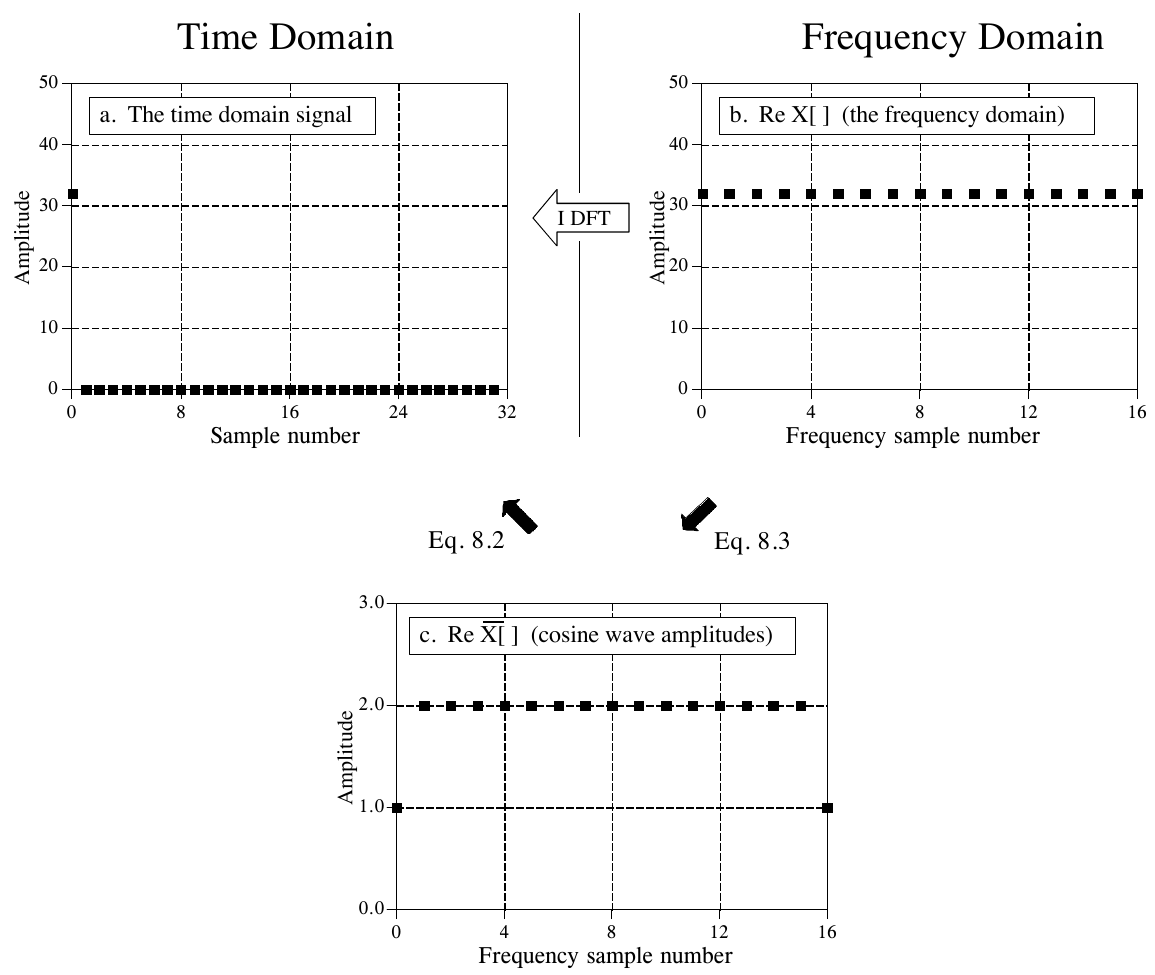
\includegraphics[width=0.963\linewidth,height=0.8\textheight,keepaspectratio]{assets/ch08/fig8-06.png}
\caption*{\textbf{图 8-6　逆 DFT 的例子。} 图 (a) 是一个示例时域信号：位于第 0
个采样、幅度为 32 的冲激。图 (b) 是这个信号频域的实部，是一个值为 32
的常数。频域的虚部（未画出）全为零。图 (c) 是用公式 8-2 重建 (a)
所需的余弦波幅度。(c) 中的值是用公式 8-3 从 (b) 求出来的。 （Time Domain
= 时域，Frequency Domain = 频域，a. The time domain signal = a.
时域信号，b. Re X{[} {]} (the frequency domain) = b. Re X{[}
{]}（频域），c.~Re X̄{[} {]} (cosine wave amplitudes) = c.~Re X̄{[}
{]}（余弦波幅度），I DFT = 逆 DFT，Eq. 8.2 / Eq. 8.3 = 公式 8-2 / 公式
8-3，Sample number = 采样序号，Frequency sample number =
频率采样序号，Amplitude = 幅度。）}
\end{figure}

图 8-6 演示了逆 DFT 的运作，以及频域和合成所需幅度之间的细微差别。图
8-6a 是我们要合成的示例信号：位于第 0 个采样、幅度为 32 的冲激。图 8-6b
是这个信号的频域表示。频域的实部是一个值为 32
的常数，虚部（未画出）全为零。下一章会讲到，这是一个重要的 DFT
变换对：时域中的冲激对应频域中的常数。眼下的要点是：(b) 是 (a) 的
DFT，(a) 是 (b) 的逆 DFT。

公式 8-3 用来把频域信号 (b) 转换成余弦波的幅度
(c)。如图所示，所有余弦波的幅度都是二，只有第 0 和第 16
个采样的值是一。本例没有画出正弦波的幅度，因为它们都为零，没有任何贡献。然后用合成方程（公式
8-2）把余弦波的幅度 (c) 转换成时域信号
(a)。（译注：原书这里写的是''(b)``，应为 (c)。）

这说明了频域和正弦波幅度有什么不同，但没有解释为什么不同。差别的原因在于，频域被定义为一种谱密度(spectral
density)。图 8-7 说明了这是怎么回事。图中的例子是一个 32
点信号频域的实部。和你预期的一样，采样从 0 到 16，代表 0 到采样率 1/2
之间等间距的 17
个频率。谱密度描述的是每单位带宽中有多少信号（幅度）。要把正弦波幅度转换成谱密度，就把每个幅度除以它所代表的带宽。于是引出下一个问题：怎样确定频域中每个离散频率的带宽？

如图所示，可以在采样之间画分界线来确定带宽。例如，第 5 个采样落在 4.5 到
5.5 之间的频带里；第 6 个采样落在 5.5 到 6.5
之间的频带里，依此类推。用总带宽（即 N/2）的分数来表示，每个采样的带宽是
2/N。例外的是两端的采样，它们的带宽只有这个的一半，即
1/N。这就解释了正弦波幅度和频域之间的 2/N
缩放因子，以及首尾两个采样需要额外的因子二。

\begin{figure}[htbp]
\centering
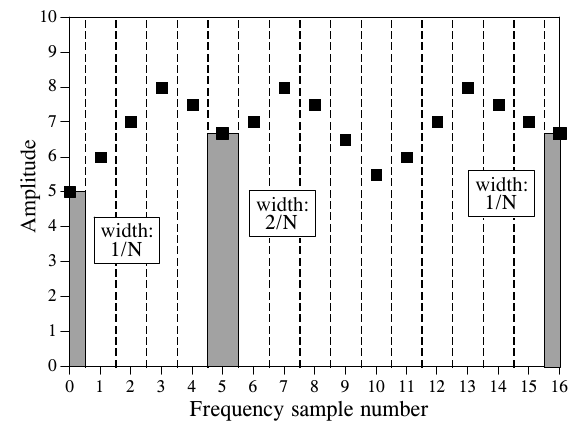
\includegraphics[width=0.483\linewidth,height=0.8\textheight,keepaspectratio]{assets/ch08/fig8-07.png}
\caption*{\textbf{图 8-7　频域采样的带宽。}
频域中的每个采样都可以看作位于一个宽度为 2/N
的频带里（用总带宽的分数表示）。例外的是第一个和最后一个采样，它们的带宽只有一半宽，即
1/N。 （Amplitude = 幅度，Frequency sample number = 频率采样序号，width
= 宽度。）}
\end{figure}

为什么要把虚部变号？这样做只是为了让实数 DFT 和它的老大哥------复数
DFT------保持一致。在第 31 章我们会说明，要让复数 DFT
的数学成立，这样做是必须的。（译注：原书这里写的是''第 29 章''，但第 29
章是《DSP 上手实践》，复数 DFT 在第 31 章，应为笔误。）只处理实数 DFT
时，很多作者不加这个负号。说起来，很多作者连 2/N
这个缩放因子都不加。你要准备好在有些讨论中看到这两样都没有。本书加上它们，有一个极其重要的理由：计算
DFT 最高效的方法是快速傅里叶变换（FFT）算法，第 12 章介绍。FFT
生成的频域就是按公式 8-2 和 8-3
定义的。如果你随意改动这些归一化因子，用到 FFT 的程序就不会按预期工作。

\section{分析：计算 DFT}

DFT
有三种完全不同的计算方法。第一，可以把问题当作一组联立方程来求解。这种方法有助于理解
DFT，但效率太低，没有实用价值。第二种方法借用上一章的一个思想：相关(correlation)。它基于在一个信号中探测一个已知波形。第三种方法叫快速傅里叶变换（FFT），是一种巧妙的算法，它把一个
N 点的 DFT 分解成 N 个各只有一个点的 DFT。FFT
通常比其他方法快几百倍。这里讨论前两种方法，FFT 是第 12
章的主题。重要的是要记住，三种方法的输出完全相同。该用哪一种？实际中，如果
DFT 少于大约 32 点，首选相关法，否则用 FFT。

\subsection{用联立方程求 DFT}

可以这样来思考 DFT 的计算。给你时域中的 N 个值，要你算出频域的 N
个值（不算那两个你知道一定为零的频域值）。初等代数给出了答案：要解出 N
个未知数，必须能写出 N
个线性无关的方程。做法是取每个正弦波的第一个采样并把它们加起来。这个和必须等于时域信号的第一个采样，这就给出了第一个方程。同样，可以对时域信号其余的每个点各写一个方程，得到所需的
N 个方程。然后用解联立方程的成熟方法，比如高斯消元法(Gauss
Elimination)，就能求出解。可惜这种方法需要极大的计算量，在 DSP
中几乎从来不用。但它在另一方面很重要：它说明了为什么能把信号分解成正弦波、需要多少个正弦波，以及基函数必须线性无关（稍后还会细说）。

\subsection{用相关求 DFT}

我们来看一种更好的方法，也是计算 DFT
的标准方法。用一个例子来说明它怎样工作。假设我们要计算一个 64 点信号的
DFT。这意味着要算出频域实部的 33 个点和虚部的 33
个点。本例只说明怎样计算一个采样 Im X{[}3{]}，即在第 0 点到第 63
点之间走完三个完整周期的正弦波的幅度。频域的其他值都用类似的方法计算。

图 8-8 演示了用相关计算 Im X{[}3{]}。图 (a) 和 (b)
是两个示例时域信号，分别叫 x1{[} {]} 和 x2{[} {]}。第一个信号 x1{[} {]}
只由一个在第 0 点到第 63 点之间走三个周期的正弦波组成。相反，x2{[} {]}
由几个正弦波和余弦波组成，没有一个在第 0 点到第 63
点之间走三个周期。这两个信号说明了计算 Im X{[}3{]}
的算法必须做到什么。输入 x1{[} {]} 时，算法必须给出
32，即信号中所含正弦波的幅度（经过公式 8-3
的缩放因子修正）。相比之下，输入另一个信号 x2{[} {]}
时，算法必须给出零，表示这个信号中没有这个特定的正弦波。（译注：按公式
8-4 带负号的定义，x1{[} {]} 实际算出来的 Im X{[}3{]} 是
−32，这里的''32''指幅度大小。本章 C 程序
\texttt{c/table8-2\_dft\_correlation.c} 实测为 −32.000000。）

相关的概念在第 7
章介绍过。回忆一下，要在一个信号中探测一个已知波形，就把两个信号相乘，再把结果信号的所有点加起来。这个过程得到的单个数值，衡量的是两个信号有多相似。图
8-8 演示了这种方法。图 (c) 和 (d) 都画出了我们要找的信号：一个在第 0
和第 63 个采样之间走 3 个周期的正弦波。图 (e) 是 (a) 和 (c)
相乘的结果。同样，(f) 是 (b) 和 (d) 相乘的结果。(e) 中所有点之和是
32，而 (f) 中所有点之和是零，说明我们找到了所需的算法。

\begin{figure}[htbp]
\centering
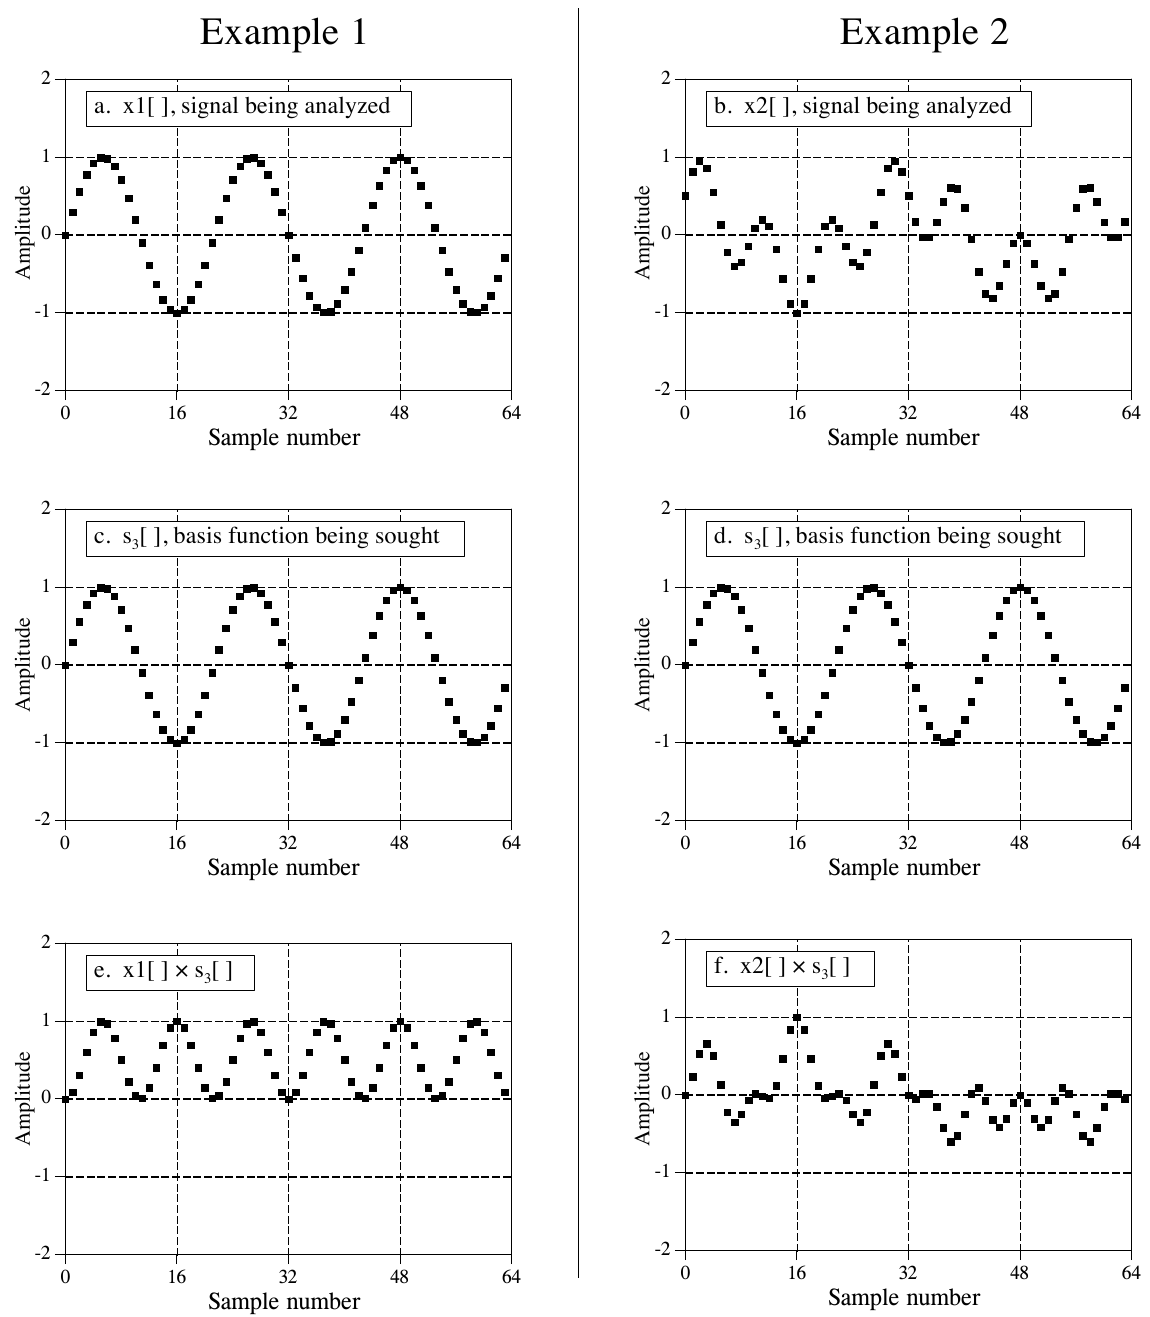
\includegraphics[width=0.958\linewidth,height=0.8\textheight,keepaspectratio]{assets/ch08/fig8-08.png}
\caption*{\textbf{图 8-8　用相关寻找基函数。} 分析两个示例信号 (a) 和
(b)，看它们是否含有 (c) 和 (d) 所示的特定基函数。图 (e) 和 (f)
是每个示例信号与基函数相乘的结果。图 (e) 的平均值为 0.5，说明 x1{[} {]}
含有这个基函数，幅度为 1.0。反过来，(f) 的平均值为零，说明 x2{[} {]}
不含这个基函数。 （Example 1 / Example 2 = 例 1 / 例 2，signal being
analyzed = 被分析的信号，basis function being sought =
要寻找的基函数，Amplitude = 幅度，Sample number = 采样序号。）}
\end{figure}

频域的其他采样用同样的方法计算。这个过程被形式化为分析方程(analysis
equation)，即从时域计算频域的数学方法：

\textbf{公式 8-4　计算 DFT 的分析方程。} 式中 x{[}i{]}
是被分析的时域信号，Re X{[}k{]} 和 Im X{[}k{]} 是要计算的频域信号。下标
i 从 0 到 N−1，下标 k 从 0 到 N/2。

\[
\mathrm{Re}\,X[k] = \sum_{i=0}^{N-1} x[i]\cos(2\pi k i/N)
\]

\[
\mathrm{Im}\,X[k] = -\sum_{i=0}^{N-1} x[i]\sin(2\pi k i/N)
\]

用文字说，频域中的每个采样，都是把时域信号乘以要找的正弦或余弦波，再把结果的各点相加得到的。如果有人问你在做什么，就自信地说：``我在把输入信号和每个基函数做相关。''表
8-2 是用这种方法计算 DFT 的计算机程序。

分析方程不需要像合成方程那样特殊处理首尾两点。不过，公式 8-4
的虚部里有一个负号。和前面一样，这个负号是为了让实数 DFT 和复数 DFT
保持一致，并不是所有书里都有。

要让这个相关算法成立，基函数必须具有一个有意思的性质：每个基函数都必须和其他所有基函数完全不相关。也就是说，任取两个基函数相乘，结果各点之和都等于零。具有这个性质的基函数叫正交的(orthogonal)。（原书误拼为
orthognal。）还有很多别的正交基函数，包括方波、三角波、冲激等。也可以用相关把信号分解到这些别的正交基函数上，就像这里用正弦波做的那样。这并不是说这样做有用，只是说它做得到。

\textbf{表 8-2}（注释已译成中文）

\begin{Shaded}
\begin{Highlighting}[]
\NormalTok{100 \textquotesingle{}THE DISCRETE FOURIER TRANSFORM}
\NormalTok{110 \textquotesingle{}频域信号 REX[ ] 和 IMX[ ] 由时域信号 XX[ ] 计算得到。}
\NormalTok{120 \textquotesingle{}}
\NormalTok{130 \textquotesingle{}}
\NormalTok{140 DIM XX[511]                       \textquotesingle{}XX[ ] 存放时域信号}
\NormalTok{150 DIM REX[256]                      \textquotesingle{}REX[ ] 存放频域的实部}
\NormalTok{160 DIM IMX[256]                      \textquotesingle{}IMX[ ] 存放频域的虚部}
\NormalTok{170 \textquotesingle{}}
\NormalTok{180 PI = 3.14159265                   \textquotesingle{}设定常数 PI}
\NormalTok{190 N\% = 512                          \textquotesingle{}N\% 是 XX[ ] 的点数}
\NormalTok{200 \textquotesingle{}}
\NormalTok{210 GOSUB XXXX                        \textquotesingle{}虚构的子程序，把数据载入 XX[ ]}
\NormalTok{220 \textquotesingle{}}
\NormalTok{230 \textquotesingle{}}
\NormalTok{240 FOR K\% = 0 TO 256                 \textquotesingle{}把 REX[ ] 和 IMX[ ] 清零，好当累加器用}
\NormalTok{250 REX[K\%] = 0}
\NormalTok{260 IMX[K\%] = 0}
\NormalTok{270 NEXT K\%}
\NormalTok{280 \textquotesingle{}}
\NormalTok{290 \textquotesingle{}                                 \textquotesingle{}把 XX[ ] 与余弦波、正弦波做相关，公式 8{-}4}
\NormalTok{300 \textquotesingle{}}
\NormalTok{310 FOR K\% = 0 TO 256                 \textquotesingle{}K\% 遍历 REX[ ] 和 IMX[ ] 中的每个采样}
\NormalTok{320 FOR I\% = 0 TO 511                 \textquotesingle{}I\% 遍历 XX[ ] 中的每个采样}
\NormalTok{330 \textquotesingle{}}
\NormalTok{340 REX[K\%] = REX[K\%] + XX[I\%] * COS(2*PI*K\%*I\%/N\%)}
\NormalTok{350 IMX[K\%] = IMX[K\%] {-} XX[I\%] * SIN(2*PI*K\%*I\%/N\%)}
\NormalTok{360 \textquotesingle{}}
\NormalTok{370 NEXT I\%}
\NormalTok{380 NEXT K\%}
\NormalTok{390 \textquotesingle{}}
\NormalTok{400 END}
\end{Highlighting}
\end{Shaded}

\textbf{C 实现}（完整可编译版本见
\texttt{c/table8-2\_dft\_correlation.c}。程序用书中有答案的例子检验：图
8-6 的冲激、图 8-8 的 x1{[} {]} 和不含 3 周期分量的信号，再把一个 512
点随机信号做 DFT 后用逆 DFT 合成回去）：

\begin{Shaded}
\begin{Highlighting}[]
\CommentTok{/* 相关法 DFT：每个频域点 = 输入信号与对应基函数的相关 */}
\DataTypeTok{static} \DataTypeTok{void}\NormalTok{ dft}\OperatorTok{(}\DataTypeTok{const} \DataTypeTok{double} \OperatorTok{*}\NormalTok{xx}\OperatorTok{,} \DataTypeTok{int}\NormalTok{ n}\OperatorTok{,} \DataTypeTok{double} \OperatorTok{*}\NormalTok{rex}\OperatorTok{,} \DataTypeTok{double} \OperatorTok{*}\NormalTok{imx}\OperatorTok{)}
\OperatorTok{\{}
    \ControlFlowTok{for} \OperatorTok{(}\DataTypeTok{int}\NormalTok{ k }\OperatorTok{=} \DecValTok{0}\OperatorTok{;}\NormalTok{ k }\OperatorTok{\textless{}=}\NormalTok{ n }\OperatorTok{/} \DecValTok{2}\OperatorTok{;}\NormalTok{ k}\OperatorTok{++)} \OperatorTok{\{}     \CommentTok{/* 240～270：REX[] 和 IMX[] 清零，当累加器用 */}
\NormalTok{        rex}\OperatorTok{[}\NormalTok{k}\OperatorTok{]} \OperatorTok{=} \FloatTok{0.0}\OperatorTok{;}
\NormalTok{        imx}\OperatorTok{[}\NormalTok{k}\OperatorTok{]} \OperatorTok{=} \FloatTok{0.0}\OperatorTok{;}
    \OperatorTok{\}}
    \ControlFlowTok{for} \OperatorTok{(}\DataTypeTok{int}\NormalTok{ k }\OperatorTok{=} \DecValTok{0}\OperatorTok{;}\NormalTok{ k }\OperatorTok{\textless{}=}\NormalTok{ n }\OperatorTok{/} \DecValTok{2}\OperatorTok{;}\NormalTok{ k}\OperatorTok{++)}        \CommentTok{/* 310：遍历频域每个点 */}
        \ControlFlowTok{for} \OperatorTok{(}\DataTypeTok{int}\NormalTok{ i }\OperatorTok{=} \DecValTok{0}\OperatorTok{;}\NormalTok{ i }\OperatorTok{\textless{}}\NormalTok{ n}\OperatorTok{;}\NormalTok{ i}\OperatorTok{++)} \OperatorTok{\{}       \CommentTok{/* 320：遍历时域每个点 */}
\NormalTok{            rex}\OperatorTok{[}\NormalTok{k}\OperatorTok{]} \OperatorTok{+=}\NormalTok{ xx}\OperatorTok{[}\NormalTok{i}\OperatorTok{]} \OperatorTok{*}\NormalTok{ cos}\OperatorTok{(}\DecValTok{2} \OperatorTok{*}\NormalTok{ PI }\OperatorTok{*}\NormalTok{ k }\OperatorTok{*}\NormalTok{ i }\OperatorTok{/}\NormalTok{ n}\OperatorTok{);}  \CommentTok{/* 340 */}
\NormalTok{            imx}\OperatorTok{[}\NormalTok{k}\OperatorTok{]} \OperatorTok{{-}=}\NormalTok{ xx}\OperatorTok{[}\NormalTok{i}\OperatorTok{]} \OperatorTok{*}\NormalTok{ sin}\OperatorTok{(}\DecValTok{2} \OperatorTok{*}\NormalTok{ PI }\OperatorTok{*}\NormalTok{ k }\OperatorTok{*}\NormalTok{ i }\OperatorTok{/}\NormalTok{ n}\OperatorTok{);}  \CommentTok{/* 350：注意负号 */}
        \OperatorTok{\}}
\OperatorTok{\}}
\end{Highlighting}
\end{Shaded}

运行结果：图 8-6 的冲激，Re X{[} {]} 全为 32、Im X{[} {]} 全为 0；图 8-8
的 x1{[} {]}，Im X{[}3{]} = −32.000000；不含 3 周期分量的信号，Im
X{[}3{]} \dspsym{≈} 3e−15（即 0）；512 点随机信号做 DFT 再逆
DFT，与原信号的最大误差约 5e−14，Im X{[}0{]} 和 Im X{[}N/2{]} 都为 0。

前面表 8-1 已经说明，逆 DFT
在程序里有两种实现方式，差别在于合成时对调内外两层循环。这不改变程序的输出，但改变你看待这个计算的方式。表
8-2 的 DFT 程序也可以这样改，把第 310～380
行的内外循环对调。和前面一样，程序的输出不变，但思考计算的方式不同。（这两种看待
DFT 和逆 DFT 的方式，可以像卷积那样，称为''输入端''和''输出端''算法。）

按表 8-2
现在的写法，它描述的是频域中的一个采样怎样受时域中所有采样的影响。也就是说，程序依次算出频域中的每个值，而不是一起算。把内外循环对调后，程序就逐个遍历时域中的采样，计算这个点对频域的贡献。整个频域就是把各个时域点的贡献加起来得到的。这引出了下一个问题：时域中的单个采样对频域提供什么样的贡献？答案在傅里叶分析一个有意思的方面里，叫对偶性(duality)。

\section{对偶性}

合成方程和分析方程（公式 8-2 和
8-4）惊人地相似。要从一个域转到另一个域，都是把已知值乘以基函数，再把乘积相加。考虑到我们得出这两个过程的方式完全不同，DFT
和逆 DFT
用的是同一种数学方法，这真是相当了不起。事实上，两个方程唯一的显著差别，源于时域是一个
N 点的信号，而频域是两个 N/2+1 点的信号。后面几章会讲到，复数 DFT
把时域和频域都表示成 N
点的复数信号。这让两个域完全对称，在两者之间转换的方程也几乎一模一样。

时域和频域之间的这种对称叫对偶性，它带来许多有意思的性质。例如，频域中的单个点对应时域中的一个正弦波。由对偶性，反过来也成立：时域中的单个点对应频域中的一个正弦波。再举一个例子，时域中的卷积对应频域中的相乘。由对偶性，反过来也成立：频域中的卷积对应时域中的相乘。第
10 章和第 11 章会更详细地讨论这些以及其他对偶关系。

\section{极坐标表示}

到目前为止，频域被描述为一组余弦波和正弦波的幅度（带一点缩放修正）。这叫直角坐标表示(rectangular
notation)。另一种方式是把频域写成极坐标形式(polar
form)。在这种表示中，Re X{[} {]} 和 Im X{[} {]} 被换成另外两个数组：X{[}
{]} 的幅值(Magnitude)，在公式中写作 Mag X{[} {]}；X{[} {]}
的相位(Phase)，写作 Phase X{[}
{]}。幅值和相位是对实部和虚部的一对一替换。例如，Mag X{[}0{]} 和 Phase
X{[}0{]} 只用 Re X{[}0{]} 和 Im X{[}0{]} 算出。同样，Mag X{[}14{]} 和
Phase X{[}14{]} 只用 Re X{[}14{]} 和 Im X{[}14{]}
算出，依此类推。要理解这种转换，想一想把同一频率的一个余弦波和一个正弦波相加会发生什么。结果是一个同频率的余弦波，但有新的幅度和新的相移(phase
shift)。写成公式，两种表示的关系是：

\textbf{公式 8-5　余弦波与正弦波相加。}
一个余弦波和一个正弦波相加，得到一个幅度和相移都不同的余弦波。A 和 B
中包含的信息被转移到另外两个变量 M 和 θ 中。

\[
A\cos(x) + B\sin(x) = M\cos(x + \theta)
\]

要点是这个过程不丢失任何信息：给定一种表示，就能算出另一种。换句话说，幅度
A 和 B 中包含的信息，同样包含在变量 M 和 θ
中。虽然这个方程涉及的是正弦波和余弦波，但它遵循的转换公式和简单的矢量一样。图
8-9 画出了类比的矢量表示：两个变量 A 和 B 可以看作直角坐标系中的量，而 M
和 θ 是极坐标中的参数。

\begin{figure}[htbp]
\centering
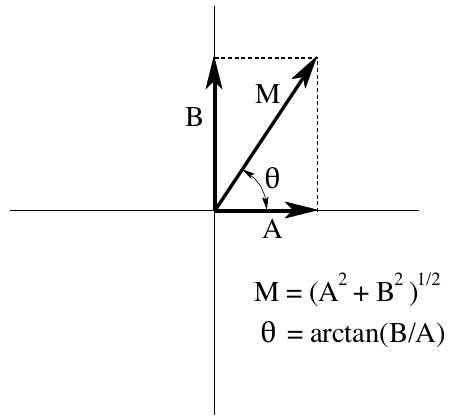
\includegraphics[width=0.383\linewidth,height=0.8\textheight,keepaspectratio]{assets/ch08/fig8-09.png}
\caption*{\textbf{图 8-9　直角坐标到极坐标的转换。}
把一个余弦波和一个（同频率的）正弦波相加，遵循的数学和简单矢量相加一样。
（图中公式：\(M = (A^2 + B^2)^{1/2}\)，\(\theta = \arctan(B/A)\)。）}
\end{figure}

在极坐标表示中，Mag X{[} {]} 存放余弦波的幅度（公式 8-5 和图 8-9 中的
M），Phase X{[} {]} 存放余弦波的相位角（公式 8-5 和图 8-9 中的
θ）。（译注：原书这里两处都写成''公式 8-4''，应为公式
8-5。）下面的公式把频域从直角坐标表示转换成极坐标表示，以及反过来：

\textbf{公式 8-6　直角坐标到极坐标的转换。} 把频域的直角坐标表示 Re
X{[}k{]} 和 Im X{[}k{]} 变成极坐标形式 Mag X{[}k{]} 和 Phase X{[}k{]}。

\[
\mathrm{Mag}\,X[k] = \left(\mathrm{Re}\,X[k]^2 + \mathrm{Im}\,X[k]^2\right)^{1/2}
\]

\[
\mathrm{Phase}\,X[k] = \arctan\!\left(\frac{\mathrm{Im}\,X[k]}{\mathrm{Re}\,X[k]}\right)
\]

\textbf{公式 8-7　极坐标到直角坐标的转换。} 把两个数组 Mag X{[}k{]} 和
Phase X{[}k{]} 转换成 Re X{[}k{]} 和 Im X{[}k{]}。

\[
\mathrm{Re}\,X[k] = \mathrm{Mag}\,X[k]\cos(\mathrm{Phase}\,X[k])
\]

\[
\mathrm{Im}\,X[k] = \mathrm{Mag}\,X[k]\sin(\mathrm{Phase}\,X[k])
\]

直角坐标和极坐标表示让你可以用两种不同的方式看待
DFT。用直角坐标表示，DFT 把一个 N 点信号分解成 N/2+1 个余弦波和 N/2+1
个正弦波，每个都有确定的幅度。用极坐标表示，DFT 把一个 N 点信号分解成
N/2+1
个余弦波，每个都有确定的幅度（叫幅值）和相移。为什么极坐标表示用余弦波而不用正弦波？因为正弦波无法表示信号的直流分量，频率为零的正弦波全是零（见图
8-5 a 和 b）。

虽然极坐标和直角坐标表示包含的信息完全相同，但很多情况下，一种比另一种好用。例如，图
8-10
用直角坐标和极坐标两种形式画出了同一个频域信号。警告：别试图看懂实部和虚部的形状，你的脑袋会爆炸！相比之下，极坐标曲线一目了然：只有大约
0.25 以下的频率存在，相移大致和频率成正比。这是一个低通滤波器(low-pass
filter)的频率响应(frequency response)。

\begin{figure}[htbp]
\centering
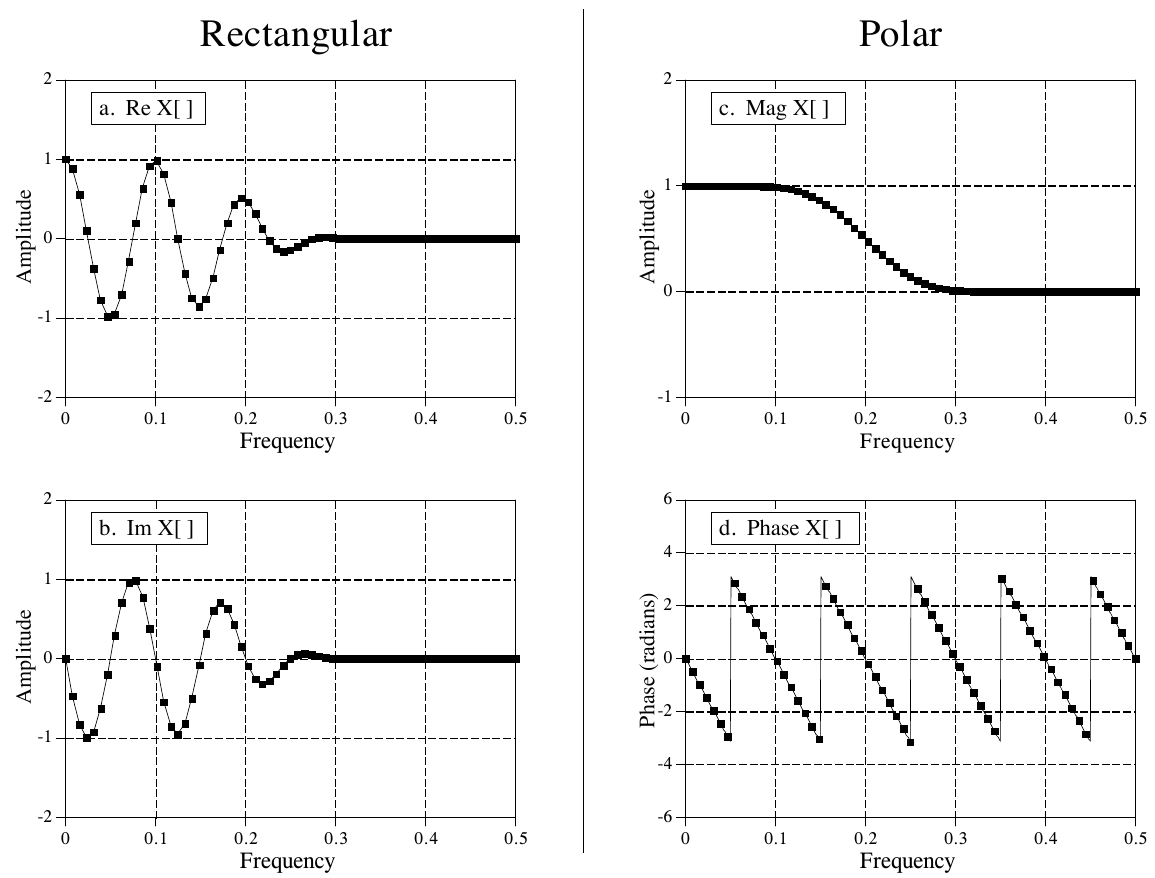
\includegraphics[width=0.963\linewidth,height=0.8\textheight,keepaspectratio]{assets/ch08/fig8-10.png}
\caption*{\textbf{图 8-10　直角坐标和极坐标频域的例子。}
本例把一个频域分别用直角坐标和极坐标表示出来。和本例一样，极坐标表示通常能让人更好地理解信号的特性。相比之下，需要做数学计算时几乎总是用直角坐标形式。特别注意，相位的第一个和最后一个采样必须为零，就像虚部一样。
（Rectangular = 直角坐标，Polar = 极坐标，Amplitude = 幅度，Phase
(radians) = 相位（弧度），Frequency = 频率。）}
\end{figure}

什么时候该用直角坐标，什么时候该用极坐标？直角坐标通常是计算（比如方程和计算机程序）的最佳选择。相比之下，图几乎总是画成极坐标形式。前面的例子表明，人几乎不可能通过看实部和虚部来理解一个频域信号的特性。在典型的程序里，频域信号一直保持直角坐标形式，直到需要给人看的时候，才做一次直角坐标到极坐标的转换。

为什么用极坐标更容易理解频域？这个问题触及了''为什么把信号分解成正弦波有用''的核心。回忆第
5
章讲的正弦保真性：正弦波进入线性系统，输出也是正弦波，并且频率和输入完全相同。只有幅度和相位会变。极坐标表示直接用各分量余弦波的幅度和相位来表示信号。相应地，系统也可以用它怎样改变每个余弦波的幅度和相位来表示。

现在想想如果在这个场景中用直角坐标会怎样。一组余弦波和正弦波的混合进入线性系统，从系统出来的也是余弦波和正弦波的混合。问题是，输入的一个余弦波可能在输出端产生余弦波和正弦波。同样，输入的一个正弦波也可能在输出端产生余弦波和正弦波。这些交叉项虽然可以理清，但整个方法和我们当初想用正弦波的初衷不相符。

\section{极坐标表示的麻烦之处}

使用极坐标表示有许多麻烦之处。没有哪个是过不去的坎，只是真的很烦人！表
8-3
是一个在直角坐标和极坐标之间转换的计算机程序，其中给出了对付其中几个麻烦的办法。

\textbf{表 8-3}（注释已译成中文）

\begin{Shaded}
\begin{Highlighting}[]
\NormalTok{100 \textquotesingle{}RECTANGULAR{-}TO{-}POLAR \& POLAR{-}TO{-}RECTANGULAR CONVERSION}
\NormalTok{110 \textquotesingle{}}
\NormalTok{120 DIM REX[256]             \textquotesingle{}REX[ ]   存放实部}
\NormalTok{130 DIM IMX[256]             \textquotesingle{}IMX[ ]   存放虚部}
\NormalTok{140 DIM MAG[256]             \textquotesingle{}MAG[ ]   存放幅值}
\NormalTok{150 DIM PHASE[256]           \textquotesingle{}PHASE[ ] 存放相位}
\NormalTok{160 \textquotesingle{}}
\NormalTok{170 PI = 3.14159265}
\NormalTok{180 \textquotesingle{}}
\NormalTok{190 GOSUB XXXX               \textquotesingle{}虚构的子程序，把数据载入 REX[ ] 和 IMX[ ]}
\NormalTok{200 \textquotesingle{}}
\NormalTok{210 \textquotesingle{}}
\NormalTok{220 \textquotesingle{}                        \textquotesingle{}直角坐标到极坐标的转换，公式 8{-}6}
\NormalTok{230 FOR K\% = 0 TO 256}
\NormalTok{240 MAG[K\%] = SQR( REX[K\%]\^{}2 + IMX[K\%]\^{}2 )                \textquotesingle{}来自公式 8{-}6}
\NormalTok{250 IF REX[K\%] = 0 THEN REX[K\%] = 1E{-}20                   \textquotesingle{}防止除以 0（麻烦 2）}
\NormalTok{260 PHASE[K\%] = ATN( IMX[K\%] / REX[K\%] )                  \textquotesingle{}来自公式 8{-}6}
\NormalTok{270 \textquotesingle{}                                                     \textquotesingle{}修正反正切（麻烦 3）}
\NormalTok{280 IF REX[K\%] \textless{} 0 AND IMX[K\%] \textless{} 0 THEN PHASE[K\%] = PHASE[K\%] {-} PI}
\NormalTok{290 IF REX[K\%] \textless{} 0 AND IMX[K\%] \textgreater{}= 0 THEN PHASE[K\%] = PHASE[K\%] + PI}
\NormalTok{300 NEXT K\%}
\NormalTok{310 \textquotesingle{}}
\NormalTok{320 \textquotesingle{}}
\NormalTok{330 \textquotesingle{}                        \textquotesingle{}极坐标到直角坐标的转换，公式 8{-}7}
\NormalTok{340 FOR K\% = 0 TO 256}
\NormalTok{350 REX[K\%] = MAG[K\%] * COS( PHASE[K\%] )}
\NormalTok{360 IMX[K\%] = MAG[K\%] * SIN( PHASE[K\%] )}
\NormalTok{370 NEXT K\%}
\NormalTok{380 \textquotesingle{}}
\NormalTok{390 END}
\end{Highlighting}
\end{Shaded}

\textbf{C 实现}（完整可编译版本见
\texttt{c/table8-3\_rect\_polar.c}。程序载入书中讨论过的几个典型点，包括
Re = 1、Im = 1 和 Re = −1、Im = −1，以及实部为 0
的点，再加一批随机点；相位与 C 标准库的 \texttt{atan2()}
对照，并检查转过去再转回来能否还原）：

\begin{Shaded}
\begin{Highlighting}[]
\PreprocessorTok{\#define NF }\DecValTok{257}\PreprocessorTok{                  }\CommentTok{/* 120～150 DIM REX[256] 等：频域 257 点 */}

\CommentTok{/* 直角 → 极坐标（公式 8{-}6），rex[] 可能被改成 1e{-}20，与原书一致 */}
\DataTypeTok{static} \DataTypeTok{void}\NormalTok{ rect\_to\_polar}\OperatorTok{(}\DataTypeTok{double} \OperatorTok{*}\NormalTok{rex}\OperatorTok{,} \DataTypeTok{const} \DataTypeTok{double} \OperatorTok{*}\NormalTok{imx}\OperatorTok{,} \DataTypeTok{double} \OperatorTok{*}\NormalTok{mag}\OperatorTok{,} \DataTypeTok{double} \OperatorTok{*}\NormalTok{phase}\OperatorTok{)}
\OperatorTok{\{}
    \ControlFlowTok{for} \OperatorTok{(}\DataTypeTok{int}\NormalTok{ k }\OperatorTok{=} \DecValTok{0}\OperatorTok{;}\NormalTok{ k }\OperatorTok{\textless{}}\NormalTok{ NF}\OperatorTok{;}\NormalTok{ k}\OperatorTok{++)} \OperatorTok{\{}          \CommentTok{/* 230 */}
\NormalTok{        mag}\OperatorTok{[}\NormalTok{k}\OperatorTok{]} \OperatorTok{=}\NormalTok{ sqrt}\OperatorTok{(}\NormalTok{rex}\OperatorTok{[}\NormalTok{k}\OperatorTok{]} \OperatorTok{*}\NormalTok{ rex}\OperatorTok{[}\NormalTok{k}\OperatorTok{]} \OperatorTok{+}\NormalTok{ imx}\OperatorTok{[}\NormalTok{k}\OperatorTok{]} \OperatorTok{*}\NormalTok{ imx}\OperatorTok{[}\NormalTok{k}\OperatorTok{]);}   \CommentTok{/* 240 */}
        \ControlFlowTok{if} \OperatorTok{(}\NormalTok{rex}\OperatorTok{[}\NormalTok{k}\OperatorTok{]} \OperatorTok{==} \DecValTok{0}\OperatorTok{)}\NormalTok{ rex}\OperatorTok{[}\NormalTok{k}\OperatorTok{]} \OperatorTok{=} \FloatTok{1e{-}20}\OperatorTok{;}    \CommentTok{/* 250：防止除零（麻烦 2） */}
\NormalTok{        phase}\OperatorTok{[}\NormalTok{k}\OperatorTok{]} \OperatorTok{=}\NormalTok{ atan}\OperatorTok{(}\NormalTok{imx}\OperatorTok{[}\NormalTok{k}\OperatorTok{]} \OperatorTok{/}\NormalTok{ rex}\OperatorTok{[}\NormalTok{k}\OperatorTok{]);}   \CommentTok{/* 260 */}
        \CommentTok{/* 270～290：修正反正切（麻烦 3），实部为负时补 ±π */}
        \ControlFlowTok{if} \OperatorTok{(}\NormalTok{rex}\OperatorTok{[}\NormalTok{k}\OperatorTok{]} \OperatorTok{\textless{}} \DecValTok{0} \OperatorTok{\&\&}\NormalTok{ imx}\OperatorTok{[}\NormalTok{k}\OperatorTok{]} \OperatorTok{\textless{}} \DecValTok{0}\OperatorTok{)}\NormalTok{  phase}\OperatorTok{[}\NormalTok{k}\OperatorTok{]} \OperatorTok{=}\NormalTok{ phase}\OperatorTok{[}\NormalTok{k}\OperatorTok{]} \OperatorTok{{-}}\NormalTok{ PI}\OperatorTok{;}  \CommentTok{/* 280 */}
        \ControlFlowTok{if} \OperatorTok{(}\NormalTok{rex}\OperatorTok{[}\NormalTok{k}\OperatorTok{]} \OperatorTok{\textless{}} \DecValTok{0} \OperatorTok{\&\&}\NormalTok{ imx}\OperatorTok{[}\NormalTok{k}\OperatorTok{]} \OperatorTok{\textgreater{}=} \DecValTok{0}\OperatorTok{)}\NormalTok{ phase}\OperatorTok{[}\NormalTok{k}\OperatorTok{]} \OperatorTok{=}\NormalTok{ phase}\OperatorTok{[}\NormalTok{k}\OperatorTok{]} \OperatorTok{+}\NormalTok{ PI}\OperatorTok{;}  \CommentTok{/* 290 */}
    \OperatorTok{\}}
\OperatorTok{\}}

\CommentTok{/* 极 → 直角坐标（公式 8{-}7） */}
\DataTypeTok{static} \DataTypeTok{void}\NormalTok{ polar\_to\_rect}\OperatorTok{(}\DataTypeTok{const} \DataTypeTok{double} \OperatorTok{*}\NormalTok{mag}\OperatorTok{,} \DataTypeTok{const} \DataTypeTok{double} \OperatorTok{*}\NormalTok{phase}\OperatorTok{,} \DataTypeTok{double} \OperatorTok{*}\NormalTok{rex}\OperatorTok{,} \DataTypeTok{double} \OperatorTok{*}\NormalTok{imx}\OperatorTok{)}
\OperatorTok{\{}
    \ControlFlowTok{for} \OperatorTok{(}\DataTypeTok{int}\NormalTok{ k }\OperatorTok{=} \DecValTok{0}\OperatorTok{;}\NormalTok{ k }\OperatorTok{\textless{}}\NormalTok{ NF}\OperatorTok{;}\NormalTok{ k}\OperatorTok{++)} \OperatorTok{\{}          \CommentTok{/* 340 */}
\NormalTok{        rex}\OperatorTok{[}\NormalTok{k}\OperatorTok{]} \OperatorTok{=}\NormalTok{ mag}\OperatorTok{[}\NormalTok{k}\OperatorTok{]} \OperatorTok{*}\NormalTok{ cos}\OperatorTok{(}\NormalTok{phase}\OperatorTok{[}\NormalTok{k}\OperatorTok{]);}    \CommentTok{/* 350 */}
\NormalTok{        imx}\OperatorTok{[}\NormalTok{k}\OperatorTok{]} \OperatorTok{=}\NormalTok{ mag}\OperatorTok{[}\NormalTok{k}\OperatorTok{]} \OperatorTok{*}\NormalTok{ sin}\OperatorTok{(}\NormalTok{phase}\OperatorTok{[}\NormalTok{k}\OperatorTok{]);}    \CommentTok{/* 360 */}
    \OperatorTok{\}}
\OperatorTok{\}}
\end{Highlighting}
\end{Shaded}

运行结果：(1, 1) \dspsym{→} 45°，(−1, −1) \dspsym{→} −135°，(−1, 1)
\dspsym{→} 135°，(0, 2) \dspsym{→} 90°，(0, −2) \dspsym{→} −90°，(−3, 0)
\dspsym{→} 180°，与 \texttt{atan2()} 完全一致；257 个点的相位与
\texttt{atan2()} 的最大差约 4e−16 弧度，直角 \dspsym{→} 极 \dspsym{→}
直角往返的最大误差约 9e−16。顺带一提，C 语言里直接用
\texttt{atan2(Im,\ Re)} 就能一次处理掉麻烦 2 和麻烦 3。

\textbf{麻烦 1：弧度还是角度}

相位可以用角度(degrees)表示，也可以用弧度(radians)表示。用角度时，相位信号的值在
−180 到 180 之间。用弧度时，每个值在 −π 到 π 之间，即 −3.141592 到
3.141592。大多数计算机语言的三角函数（余弦、正弦、反正切等）都要求用弧度。和这些长长的小数打交道很烦人，得到的数据也不好解读。例如，如果你想给信号加上
90 度相移，就得给相位加
1.570796。在程序里敲这个数要不了你的命，但确实很烦。处理这个问题最好的办法是在程序开头定义常数
PI = 3.141592，这样 90 度相移就可以写成 PI/2。角度和弧度在 DSP
中都很常用，两样你都得习惯。

\textbf{麻烦 2：除以零错误}

把直角坐标转换成极坐标时，经常会遇到实部为零、虚部不为零的频率。这只是说明相位恰好是
90 度或 −90 度。可你试试跟计算机说这个！程序用
\(\mathrm{Phase}\,X[k] = \arctan(\mathrm{Im}\,X[k]/\mathrm{Re}\,X[k])\)
计算相位时，会发生除以零错误。即使程序没有因此停止，这个频率得到的相位也不对。要避免这个问题，必须在做除法前检查实部是否为零。如果是零，就要检查虚部是正还是负，分别把相位设为
π/2 或
−π/2。最后，还得绕过这次除法。这些步骤都不难，只是可能让人恼火。表 8-3
第 250
行给出了另一种处理办法：如果实部为零，就把它改成一个小到可以忽略的数，让数学运算器在做除法时不出错。

\textbf{麻烦 3：反正切算错}

考虑一个频域采样，Re X{[}k{]} = 1，Im X{[}k{]} = 1。公式 8-6
给出对应的极坐标值 Mag X{[}k{]} = 1.414，Phase X{[}k{]} =
45°。再考虑另一个采样，Re X{[}k{]} = −1，Im X{[}k{]} = −1。公式 8-6
给出的仍然是 Mag X{[}k{]} = 1.414，Phase X{[}k{]} =
45°。问题是，这个相位是错的！它应该是
−135°。只要实部为负，就会出这个错。纠正的办法是在算出相位之后检查实部和虚部。如果实部和虚部都为负，就从算出的相位中减去
180°（即 π 弧度）。如果实部为负、虚部为正，就加上 180°（即 π 弧度）。表
8-3 程序的第 280 和 290 行展示了怎样做。（译注：原书这里写的是''第 340
和 350 行''，但那两行是极坐标到直角坐标的转换，做修正的是第 280 和 290
行。）如果你没注意到这个问题，算出的相位就只会在 −π/2 到 π/2
之间，而不是在 −π 到 π 之间。把这一点牢牢记住。如果你看到相位只延伸到
±1.5708，那就是你忘了纠正反正切计算中的歧义。

\textbf{麻烦 4：极小幅值的相位}

设想下面这个场景。你正埋头做某个 DSP
任务，突然发现相位有一部分看起来不对劲。它可能有噪声，可能乱跳，也可能干脆就是错的。你花了一个小时翻看几百行代码，终于找到了答案：对应的幅值太小，被淹没在舍入噪声(round-off
noise)里了。如果幅值小到可以忽略，相位就没有任何意义，可能取到奇怪的值。图
8-11
就是一个例子。幅度信号淹没在噪声里时，通常一眼就能看出来；那些值小得让你不得不怀疑它们没有意义。相位就不一样了。极坐标信号被噪声污染时，相位的值是
−π 到 π
之间的随机数。不幸的是，这往往看起来像个真实的信号，而不是它实际上的无意义数据。

\begin{figure}[htbp]
\centering
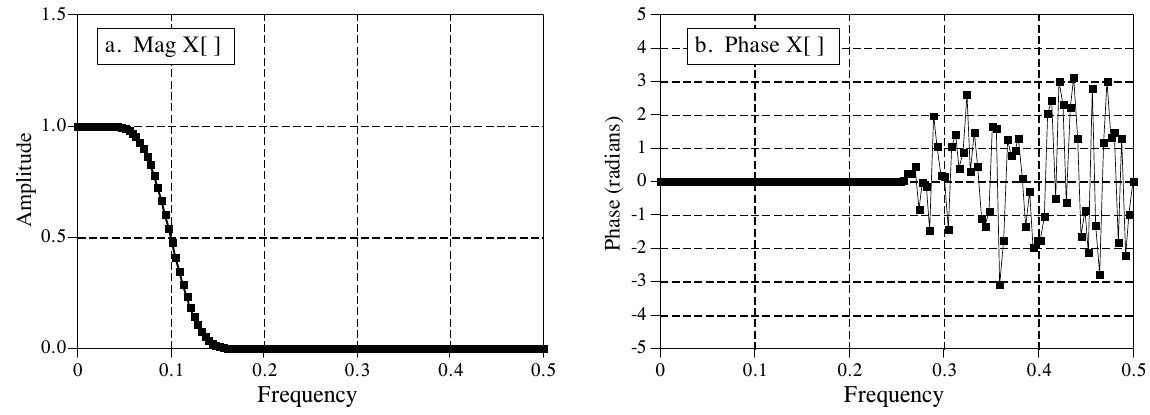
\includegraphics[width=0.958\linewidth,height=0.8\textheight,keepaspectratio]{assets/ch08/fig8-11.png}
\caption*{\textbf{图 8-11　小幅值信号的相位。}
在幅值降到很低的频率处，舍入噪声会让相位大幅乱跳。别误以为这是一个有意义的信号。
（Amplitude = 幅度，Phase (radians) = 相位（弧度），Frequency = 频率。）}
\end{figure}

\textbf{麻烦 5：相位的 2π 歧义}

再看一看图 8-10d，注意数据中的几处不连续。每当一个点看起来要降到
−3.141592 以下时，它就跳回到 3.141592。（译注：原书这里把前一个数印成了
−3.14592。）这是正弦波周期性造成的。例如，相移 θ 和相移 θ + 2π、θ +
4π、θ + 6π 等等完全一样。给相位加上 2π
的任意整数倍，任何正弦波都不变。信号中这些表面上的不连续，是计算机算法从无穷多个等价的可能中挑了它喜欢的那个的结果。它总是选最小的那个值，让相位保持在
−π 到 π 之间。

如果相位没有这些不连续，通常更容易理解，即使这意味着相位会超过 π 或低于
−π。这叫相位展开(unwrapping the phase)，图 8-12 是一个例子。如表 8-4
的程序所示，给相位的每个值加上或减去 2π
的某个整数倍。具体的值由一个让相邻采样之差最小的算法决定。

\begin{figure}[htbp]
\centering
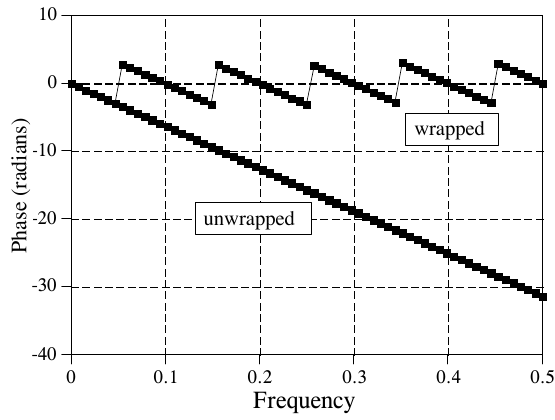
\includegraphics[width=0.463\linewidth,height=0.8\textheight,keepaspectratio]{assets/ch08/fig8-12.png}
\caption*{\textbf{图 8-12　相位展开的例子。}
上面的曲线是直角坐标到极坐标转换程序得到的典型相位信号。信号中的每个值都必须在
−π 和 π 之间（即 −3.14159 和
3.14159）。如下面的曲线所示，可以给每个采样加上或减去 2π
的整数倍来展开相位，整数的选取要让点与点之间的不连续最小。 （Phase
(radians) = 相位（弧度），Frequency = 频率，wrapped =
卷绕的（未展开），unwrapped = 展开后的。）}
\end{figure}

\textbf{表 8-4}（注释已译成中文）

\begin{Shaded}
\begin{Highlighting}[]
\NormalTok{100 \textquotesingle{} PHASE UNWRAPPING}
\NormalTok{110 \textquotesingle{}}
\NormalTok{120 DIM PHASE[256]         \textquotesingle{}PHASE[ ] 存放原始相位}
\NormalTok{130 DIM UWPHASE[256]       \textquotesingle{}UWPHASE[ ] 存放展开后的相位}
\NormalTok{140 \textquotesingle{}}
\NormalTok{150 PI = 3.14159265}
\NormalTok{160 \textquotesingle{}}
\NormalTok{170 GOSUB XXXX             \textquotesingle{}虚构的子程序，把数据载入 PHASE[ ]}
\NormalTok{180 \textquotesingle{}}
\NormalTok{190 UWPHASE[0] = 0         \textquotesingle{}所有相位信号的第一个点都是零}
\NormalTok{200 \textquotesingle{}}
\NormalTok{210 \textquotesingle{}                      \textquotesingle{}执行展开算法}
\NormalTok{220 FOR K\% = 1 TO 256}
\NormalTok{230 C\% = CINT( (UWPHASE[K\%{-}1] {-} PHASE[K\%]) / (2 * PI) )}
\NormalTok{240 UWPHASE[K\%] = PHASE[K\%] + C\%*2*PI}
\NormalTok{250 NEXT K\%}
\NormalTok{260 \textquotesingle{}}
\NormalTok{270 END}
\end{Highlighting}
\end{Shaded}

\textbf{C 实现}（完整可编译版本见
\texttt{c/table8-4\_phase\_unwrap.c}。程序按图 8-12
的样子生成数据：一条从 0 线性降到 −10π（约 −31.4）的真实相位，相当于延迟
10 个采样点；把它折回 −π～π 作为输入，展开后与真实相位对照）：

\begin{Shaded}
\begin{Highlighting}[]
\PreprocessorTok{\#define NF }\DecValTok{257}\PreprocessorTok{                  }\CommentTok{/* 120～130 DIM PHASE[256]、UWPHASE[256] */}

\NormalTok{    uwphase}\OperatorTok{[}\DecValTok{0}\OperatorTok{]} \OperatorTok{=} \DecValTok{0}\OperatorTok{;}                         \CommentTok{/* 190：所有相位信号的第一点都是 0 */}
    \ControlFlowTok{for} \OperatorTok{(}\DataTypeTok{int}\NormalTok{ k }\OperatorTok{=} \DecValTok{1}\OperatorTok{;}\NormalTok{ k }\OperatorTok{\textless{}}\NormalTok{ NF}\OperatorTok{;}\NormalTok{ k}\OperatorTok{++)} \OperatorTok{\{}          \CommentTok{/* 220 */}
        \CommentTok{/* 230：CINT 是四舍五入取整，算出要补几个 2π */}
        \DataTypeTok{long}\NormalTok{ c }\OperatorTok{=}\NormalTok{ lround}\OperatorTok{((}\NormalTok{uwphase}\OperatorTok{[}\NormalTok{k }\OperatorTok{{-}} \DecValTok{1}\OperatorTok{]} \OperatorTok{{-}}\NormalTok{ phase}\OperatorTok{[}\NormalTok{k}\OperatorTok{])} \OperatorTok{/} \OperatorTok{(}\DecValTok{2} \OperatorTok{*}\NormalTok{ PI}\OperatorTok{));}
\NormalTok{        uwphase}\OperatorTok{[}\NormalTok{k}\OperatorTok{]} \OperatorTok{=}\NormalTok{ phase}\OperatorTok{[}\NormalTok{k}\OperatorTok{]} \OperatorTok{+}\NormalTok{ c }\OperatorTok{*} \DecValTok{2} \OperatorTok{*}\NormalTok{ PI}\OperatorTok{;} \CommentTok{/* 240 */}
    \OperatorTok{\}}
\end{Highlighting}
\end{Shaded}

运行结果：展开后最后一点（频率 0.5）为 −31.4159，与真实值 −10π
一致；全部 257 点与真实相位的最大误差约 2e−15。

\textbf{麻烦 6：幅值总是正的（相位的 π 歧义）}

图 8-13
用直角坐标和极坐标两种形式画出了一个频域信号。实部平滑，很容易理解，虚部则全为零。相比之下，极坐标信号里有突然的不连续和尖角。这是因为按定义，幅值必须总是正的。每当实部降到零以下，幅值就通过把相位改变
π（或
−π，两者是一回事）来保持为正。这对数学来说不是问题，但不规则的曲线可能很难解读。

\begin{figure}[htbp]
\centering
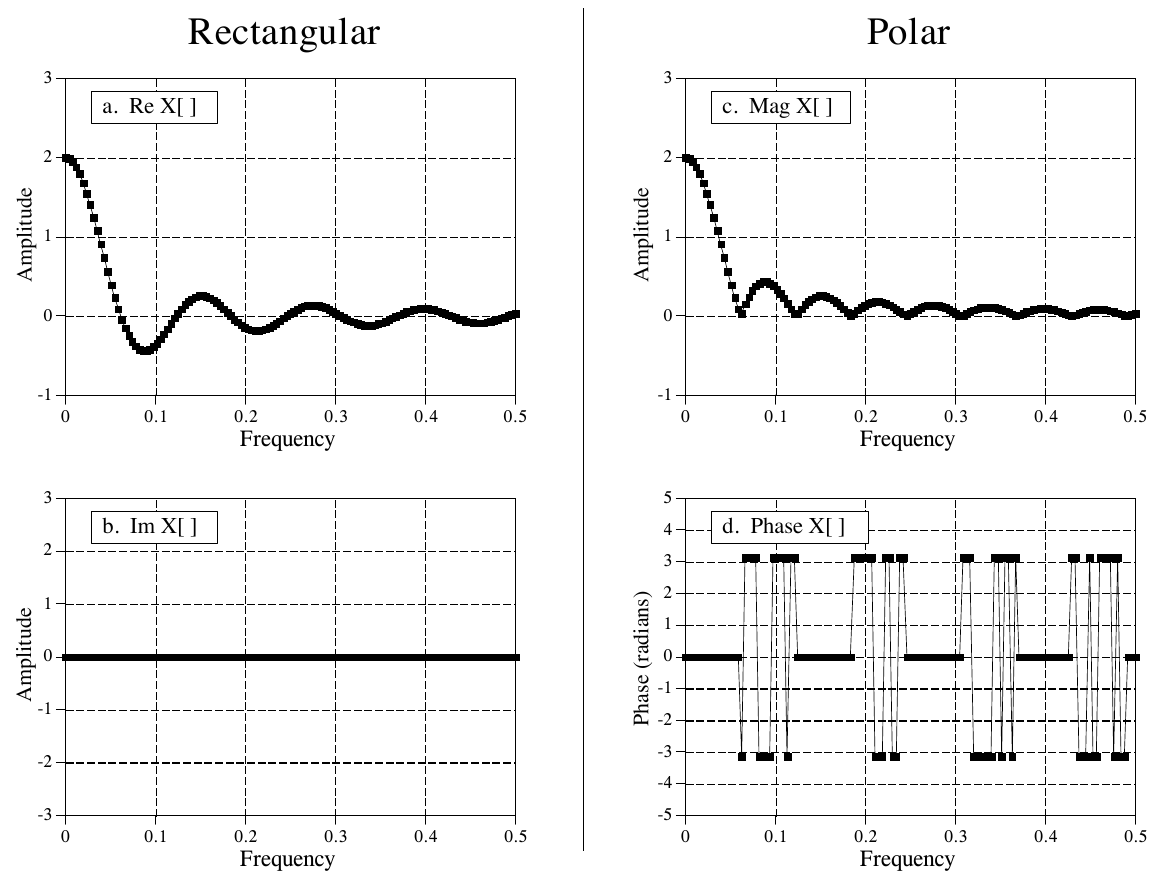
\includegraphics[width=0.963\linewidth,height=0.8\textheight,keepaspectratio]{assets/ch08/fig8-13.png}
\caption*{\textbf{图 8-13　直角坐标和极坐标形式的示例信号。}
由于幅值（按定义）必须总是正的，幅值和相位可能出现突然的不连续和尖角。图
(d) 还展示了另一个麻烦：随机噪声会让相位在 π 和 −π 之间快速来回跳。
（Rectangular = 直角坐标，Polar = 极坐标，Amplitude = 幅度，Phase
(radians) = 相位（弧度），Frequency = 频率。）}
\end{figure}

一个解决办法是允许幅值取负值。在图 8-13
的例子里，这会让幅值看起来和实部一样，而相位全为零。如果这有助于你理解，这样做没什么不对。只是要小心，别把带负值的信号叫做''幅值''，因为这违反了它的正式定义。本书用一个含糊其辞的说法------展开幅值(unwrapped
magnitude)------来表示允许取负值的''幅值''。

\textbf{麻烦 7：π 和 −π 之间的尖刺}

由于 π 和 −π
代表同一个相移，舍入噪声会让相位中相邻的点在这两个值之间快速来回切换。如图
8-13d
所示，这会在本来平滑的曲线上造成急剧的断点和尖刺。别被骗了，相位其实并没有这么不连续。

% !TEX root = ../main.tex
% 本文件由 build-tex.sh 从 09-DSP指南-第9章中译.md 生成，改内容请改 md 后重新生成

\chapter{DFT 的应用}\label{ch-09}

离散傅里叶变换（Discrete Fourier
Transform，DFT）是数字信号处理中最重要的工具之一。本章讨论它的三种常见用法。第一，DFT
可以计算信号的频谱(frequency
spectrum)。这是直接考察编码在各正弦分量的频率、相位和幅度中的信息。例如，人的语音和听觉用的就是这种编码方式的信号。第二，DFT
可以由系统的冲激响应求出系统的频率响应(frequency
response)，反过来也行。这让我们可以在频域里分析系统，就像卷积让我们可以在时域里分析系统一样。第三，DFT
可以作为更复杂的信号处理技术中的一个中间步骤。最经典的例子是 FFT
卷积(FFT convolution)，一种比常规方法快几百倍的卷积算法。

\section{信号的频谱分析}

信息编码在构成信号的正弦波里，这种情况非常普遍。自然产生的信号是这样，人造的信号也是这样。我们的宇宙里有许多东西在振荡。例如，语音来自人的声带振动；恒星和行星绕自身的轴自转、彼此绕转时，亮度会发生变化；船的螺旋桨让水产生周期性的位移，等等。对这些信号来说，时域波形的形状并不重要，关键信息在各正弦分量的频率、相位和幅度里。DFT
就是用来提取这些信息的。

举个例子来说明。假设我们想研究在海洋中传播的声音。首先，把一个麦克风放进水里，把得到的电信号放大到合适的电平，比如几伏。然后用一个模拟低通滤波器去掉
80 赫兹以上的所有频率，这样信号就能以每秒 160
个采样的速率数字化。采集并存储了几千个采样之后，下一步做什么？

第一件事就是看看数据。图 9-1a 是我们这个假想实验中的 256
个采样。能看到的只是一个满是噪声的波形，人眼从中看不出什么信息。出于稍后会解释的原因，下一步是把这个信号乘以一条叫汉明窗(Hamming
window)的平滑曲线，见 (b)。（第 16 章给出了汉明窗和其他窗的公式，见公式
16-1、16-2 和图 16-2a。）这样得到一个 256
点的信号，两端附近的采样幅度被压低了，见 (c)。

做 DFT 并转换成极坐标形式，得到 (d) 中 129
点的频谱。遗憾的是，它看起来也是一团乱糟糟的噪声。这是因为原来 256
个点里没有足够的信息，得不到一条规整的曲线。用更长的 DFT
对这个问题毫无帮助。例如，用 2048 点 DFT，频谱就有 1025 个采样。虽然原来
2048
个点包含更多信息，但频谱里采样数也按同样倍数增加，把信息摊薄了。更长的
DFT 提供更好的频率分辨率(frequency resolution)，但噪声水平不变。

办法是用更多的原始信号，同时不增加频谱的点数。具体做法是把输入信号切成许多段
256 点的片段。每段都乘以汉明窗，做 256 点
DFT，转换成极坐标形式。然后把得到的这些频谱取平均，形成一个 129
点的频谱。图 (e) 是对 100 个像 (d)
那样的频谱取平均的例子。改善是显而易见的：噪声降到了能看出信号有趣特征的水平。用这种方式取平均的只是频域的幅度；相位通常丢掉，因为它不含有用的信息。随机噪声按段数的平方根成比例减小。100
段比较典型，有些应用为了让微弱的特征显现出来，可能要对几百万段取平均。

还有第二种降低频谱噪声的方法。先做一个非常长的 DFT，比如 16,384
点。得到的频谱分辨率很高（8193
个采样），但噪声很大。再用一个低通数字滤波器把频谱平滑一下，以牺牲分辨率为代价降低噪声。例如，最简单的数字滤波器可以把原始频谱中
64
个相邻采样取平均，作为滤波后频谱的一个采样。算一算就知道，这和第一种方法给出的噪声与分辨率大致相同------相当于把
16,384 个点切成 64 段、每段 256 点。

该用哪种方法？第一种更容易，因为不需要数字滤波器。第二种有可能性能更好，因为可以对数字滤波器进行定制，优化噪声与分辨率之间的取舍。不过，这点性能提升很少值得费这个劲。因为噪声和分辨率都可以靠使用更多的输入数据来改善。例如，设想把采集到的数据切成
10,000 段，每段 16,384 个采样。这样得到的频谱分辨率高（8193
点），噪声也低（10,000
次平均）。问题解决了！因此，本章的讨论只看分段平均法。

\begin{figure}[htbp]
\centering
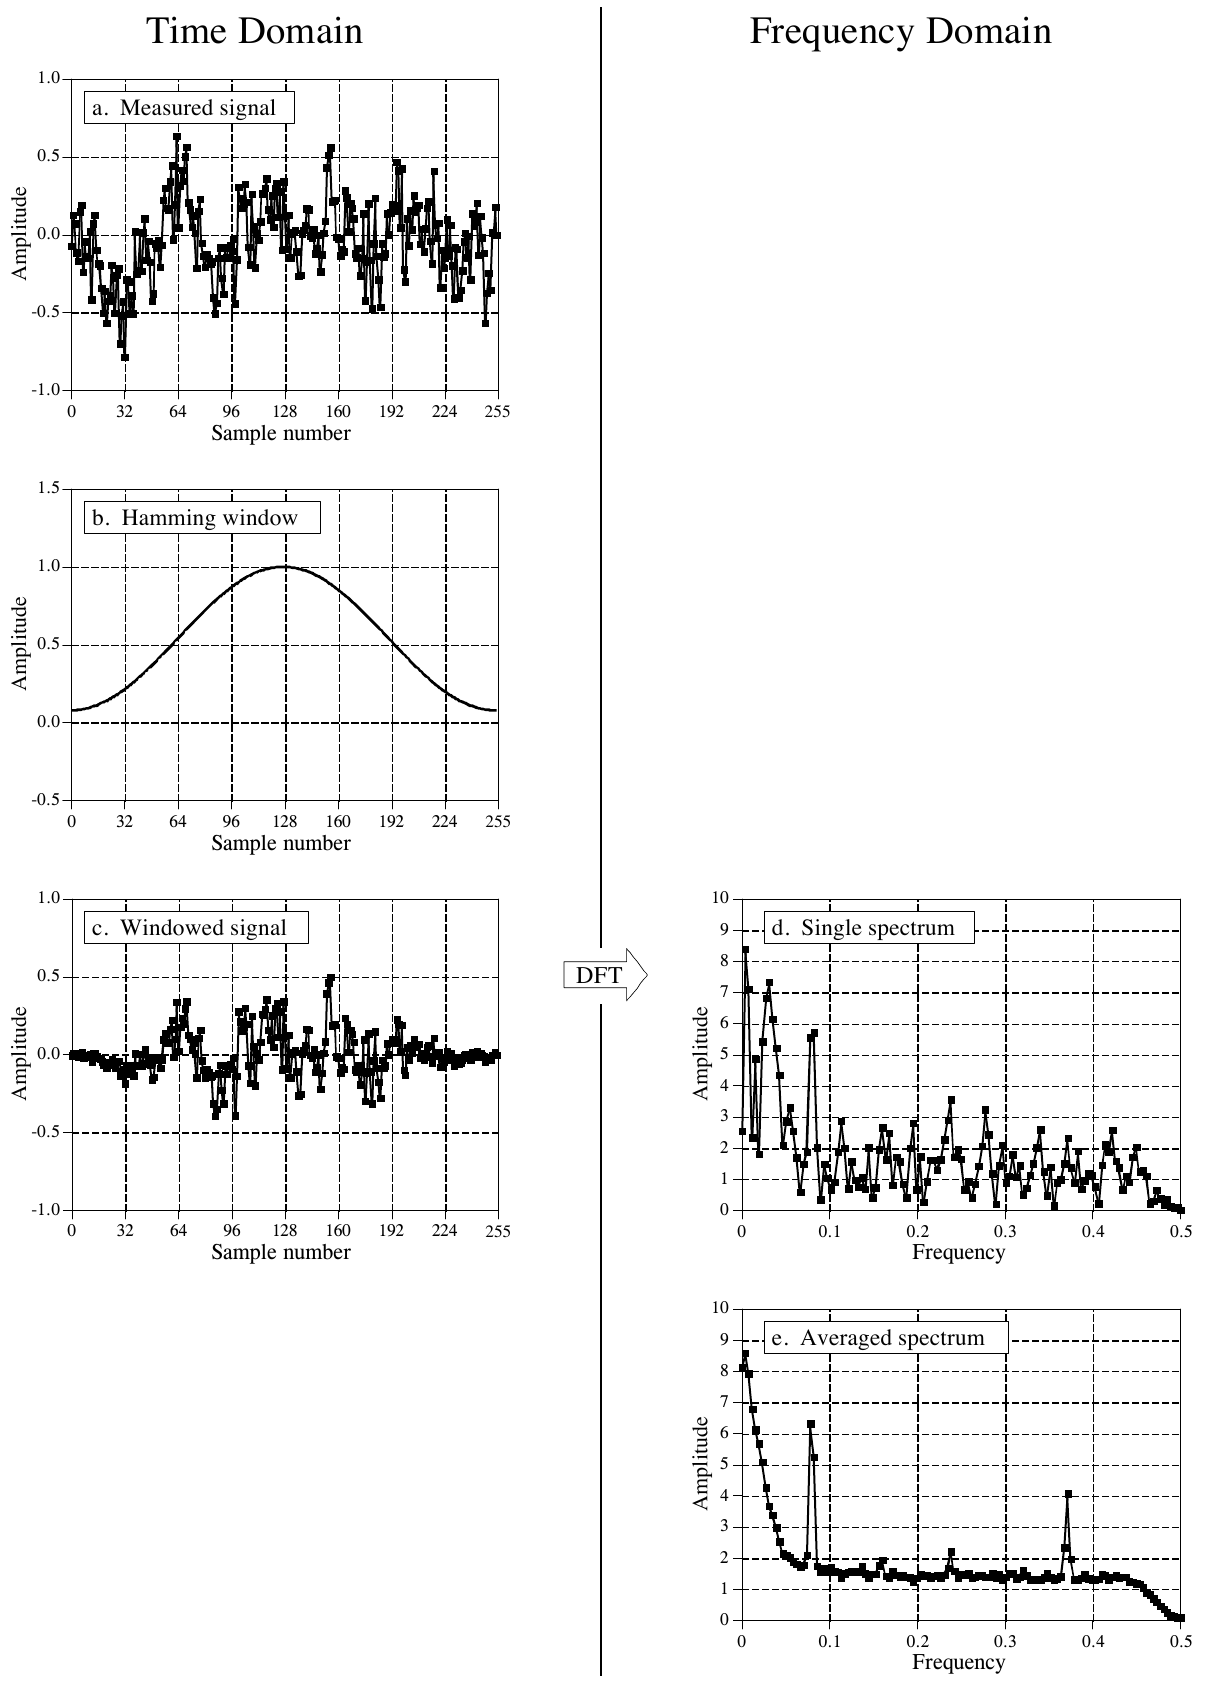
\includegraphics[width=1.000\linewidth,height=0.8\textheight,keepaspectratio]{assets/ch09/fig9-01.png}
\caption*{\textbf{图 9-1　频谱分析的一个例子。} (a) 是以每秒 160
个采样的速率从一个（模拟的）水下麦克风采得的 256 个采样。这个信号乘以
(b) 中的汉明窗，得到 (c) 中加窗后的信号。用 DFT
求出加窗信号的频谱，显示在 (d) 中（只画幅度）。对 100
个这样的频谱取平均可以降低随机噪声，得到 (e) 中的平均频谱。 （Time
Domain = 时域，Frequency Domain = 频域；a. Measured signal =
测得的信号；b. Hamming window = 汉明窗；c.~Windowed signal =
加窗后的信号；d.~Single spectrum = 单次频谱；e. Averaged spectrum =
平均频谱。Amplitude = 幅度，Sample number = 采样序号，Frequency =
频率。原书图注排在左下角空白处，裁图时已去掉，译文见上。）}
\end{figure}

图 9-2
是我们这个水下麦克风的一个频谱示例，展示了采集到的信号的频谱中常见的几种特征。先别管那些尖峰。在
10 到 70 赫兹之间，信号是一段比较平坦的区域。这叫白噪声(white
noise)，因为它包含等量的所有频率，就像白光一样。它源于时域波形上的噪声在采样之间互不相关(uncorrelated)。也就是说，知道某一个采样上的噪声值，对其他任何采样上的噪声值都提供不了任何信息。例如，电子电路中电子的随机运动就会产生白噪声。举个更熟悉的例子，淋浴时水花打在地上的声音就是白噪声。图
9-2 中的白噪声可能来自好几个源头，包括模拟电子电路，或者海洋本身。

70 赫兹以上，白噪声的幅度迅速下降。这是抗混叠滤波器(antialias
filter)滚降(roll-off)的结果。理想的滤波器会让 80
赫兹以下的所有频率通过，挡住以上的所有频率。实际上不可能做到完全陡峭的截止，你应该会看到这种逐渐的下降。如果没看到，就要怀疑出现了混叠问题。

大约 10 赫兹以下，噪声迅速上升，这是由一种叫 1/f 噪声（1/f noise，读作
one-over-f noise）的奇特现象造成的。1/f
噪声是个谜。人们在非常不同的系统里都测到过它，比如高速公路上的车流密度和晶体管里的电子噪声。只要看到足够低的频率，大概在所有系统里都能测到它。尽管它这么普遍，研究者至今没有得出关于
1/f
噪声的一般理论和认识。在某些具体系统里，这种噪声的成因是可以确定的；但这并没有回答为什么
1/f 噪声无处不在。对常见的模拟电子电路和大多数物理系统来说，白噪声和 1/f
噪声的分界大约在 1 到 100 赫兹之间。

\begin{figure}[htbp]
\centering
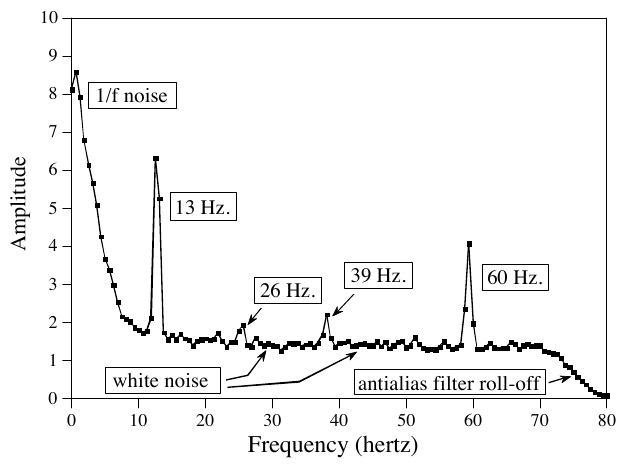
\includegraphics[width=0.517\linewidth,height=0.8\textheight,keepaspectratio]{assets/ch09/fig9-02.png}
\caption*{\textbf{图 9-2　频谱示例。} 采集到的信号的频谱中会出现三类特征：(1)
随机噪声，比如白噪声和 1/f 噪声；(2)
干扰信号，来自电源线、开关电源、广播电视台、微音效应等；(3)
真正的信号，通常表现为一个基频加上若干谐波。这个示例频谱（只画幅度）展示了其中几种特征。
（1/f noise = 1/f 噪声，white noise = 白噪声，antialias filter roll-off
= 抗混叠滤波器的滚降；13 Hz.、26 Hz.、39 Hz.、60 Hz.
为各峰的频率。Amplitude = 幅度，Frequency (hertz) =
频率（赫兹）。原书图注排在左侧，裁图时已去掉，译文见上。）}
\end{figure}

现在来看图 9-2 中的尖峰。最容易解释的是 60
赫兹那个，它是市电造成的电磁干扰。由于电源线的波形不是完美的正弦波，还应该会在这个频率的倍数（120、180、240
赫兹等）处看到较小的峰。在 25～40 kHz
之间也常能看到干扰峰，这是开关电源设计者偏爱的频段。附近的广播和电视台会在兆赫范围产生干扰峰。系统中的部件受到震动时也会振动，造成低频峰。这叫微音效应(microphonics)，通常在
10 到 100 赫兹产生峰。

现在来看真正的信号。在 13 赫兹有一个很强的峰，26 和 39
赫兹有较弱的峰。下一章会讲到，这是一个非正弦的周期波形的频谱。13
赫兹的峰叫基频(fundamental frequency)，26 和 39
赫兹的峰分别叫二次谐波和三次谐波(harmonic)。你还会预期在 13
赫兹的其他倍数处找到峰，比如 52、65、78 赫兹等。在图 9-2
中看不到它们，是因为它们被埋在白噪声里了。例如，这个 13
赫兹的信号可能是一艘潜艇的三叶螺旋桨以每秒 4.33
转旋转产生的。这正是被动声呐(passive
sonar)的原理：根据水下声音的频率和谐波成分来识别它们。

假设有几个峰靠得很近，如图 9-3
所示。有两个因素限制了能得到的频率分辨率，也就是峰能靠多近而不合并成一个。第一个因素是
DFT 的长度。N 点 DFT 产生的频谱由 N/2 + 1
个采样组成，均匀分布在零到采样频率的一半之间。要分开两个靠得很近的频率，采样间距必须小于两个峰之间的距离。例如，512
点 DFT 足以分开图 9-3 中的两个峰，而 128 点 DFT 不行。

\begin{figure}[htbp]
\centering
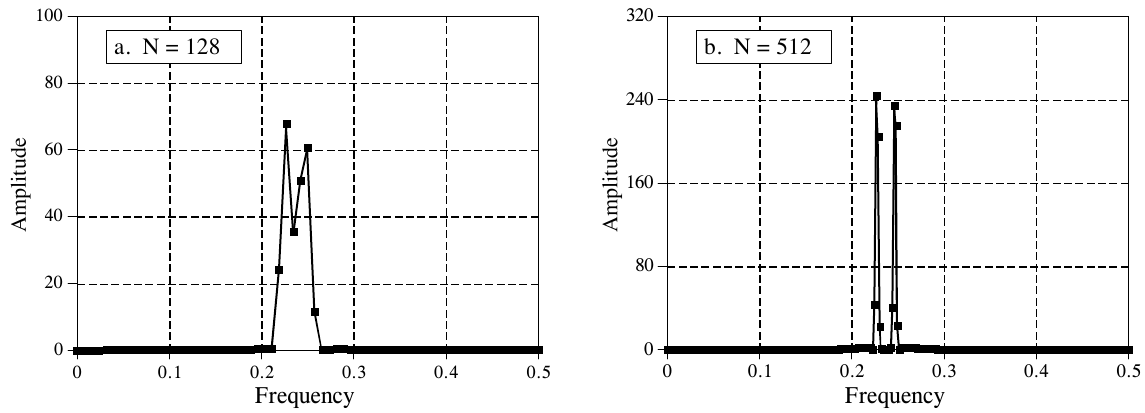
\includegraphics[width=0.954\linewidth,height=0.8\textheight,keepaspectratio]{assets/ch09/fig9-03.png}
\caption*{\textbf{图 9-3　频谱的分辨率。} DFT
越长，分开靠得很近的特征的能力越强。在这几个示例幅度谱中，128 点 DFT
分辨不出两个峰，而 512 点 DFT 可以。 （a. N = 128；b. N = 512。Amplitude
= 幅度，Frequency = 频率。）}
\end{figure}

限制分辨率的第二个因素更微妙。设想一个信号，由两个频率只差一点点的正弦波相加而成。在这个信号的一小段上，比如几个周期内，波形看起来就像一个单一的正弦波。两个频率越接近，这一段就必须越长，才能断定存在不止一个频率。换句话说，信号的长度限制了频率分辨率。这与第一个因素不同，因为输入信号的长度不必与
DFT 的长度相同。例如，一个 256 点的信号可以补零到 2048 点长。做 2048 点
DFT 得到 1025
个采样的频谱。补进去的零不改变频谱的形状，只是在频域里提供了更多的采样。尽管采样这么密，分开靠近的峰的能力只比用
256 点 DFT 好一点点。当 DFT
与输入信号等长时，分辨率受这两个因素的限制大约相当。我们稍后会再回到这个问题。

下一个问题：如果输入信号中含有一个频率位于两个基函数之间的正弦波，会怎样？图
9-4a
给出了答案。这是一个由两个正弦波组成的信号的频谱，其中一个的频率与某个基函数(basis
function)相同，另一个的频率在两个基函数之间。正如你所预期的，第一个正弦波表示为单独一个点。另一个峰比较难理解。由于它不能用单个采样表示，就变成了一个带有尾巴、尾巴延伸得很远的峰。

解决办法？像前面讲过的那样，在做 DFT 之前把信号乘以汉明窗。图 (b)
表明，加窗以后频谱在三个方面发生了变化。第一，两个峰变得更相像了。这是好事。第二，尾巴大大减小了。这也是好事。第三，窗让峰变宽，降低了频谱的分辨率。这是坏事。用
DSP 的行话说，窗在分辨率（峰的宽度）与频谱泄漏(spectral
leakage)（尾巴的幅度）之间提供了一种取舍。

\begin{figure}[htbp]
\centering
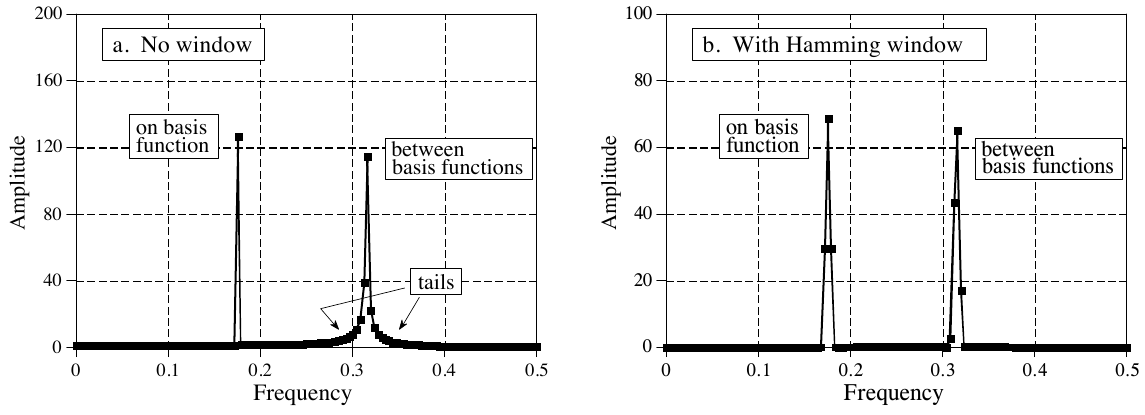
\includegraphics[width=0.954\linewidth,height=0.8\textheight,keepaspectratio]{assets/ch09/fig9-04.png}
\caption*{\textbf{图 9-4　在频谱分析中使用窗的例子。} (a)
是一个由两个正弦波组成的信号的频谱（只画幅度）。一个正弦波的频率恰好等于某个基函数，因此可以用单个采样表示；另一个的频率在两个基函数之间，导致峰带有尾巴。(b)
是同一个信号在做 DFT
之前加窗后的频谱。窗使两个峰看起来一样并减小了尾巴，但使峰变宽了。 （a.
No window = 不加窗；b. With Hamming window = 加汉明窗；on basis function
= 落在基函数上，between basis functions = 位于两个基函数之间，tails =
尾巴。Amplitude = 幅度，Frequency = 频率。）}
\end{figure}

\begin{quote}
\textbf{译注：} 原书图 9-4 的图注写的是 ``with a Blackman window
applied''（加布莱克曼窗），但正文和子图 (b) 的标签都是汉明窗(Hamming
window)。这里按正文和子图译作汉明窗。
\end{quote}

为了更详细地探讨其中的理论，设想一个无限长的离散正弦波，频率为采样率的
0.1。这个信号的频谱是一个无限窄的峰，其他所有频率都为零。当然，这个信号和它的频谱都无法放进数字计算机，因为一个无限长、一个无限窄。为了绕过这一点，我们从两个方面改变这个信号，这两方面都会使真实频谱失真。

第一，用一个窗去乘信号，从而截断信号中的信息。例如，一个 256
点的矩形窗(rectangular window)让 256
个点保留原值，而这个无限长信号中的其他所有采样都被设为零。同样，汉明窗除了把窗外的点都设为零以外，还会对保留下来的采样进行整形。这个信号仍然是无限长的，但只有有限个采样的值不为零。

这种加窗对频域有什么影响？第 10
章会讲到，两个时域信号相乘时，对应的频域是相卷积的。由于原来的频谱是一个无限窄的峰（即冲激函数），加窗信号的频谱就是窗的频谱平移到这个峰所在的位置。图
9-5
展示了用四种不同的窗时频谱峰会是什么样子。（如果需要复习分贝(dB)，可以先看第
14 章。）图 9-5a 是矩形窗的结果。(b) 和 (c)
是两种常用的窗------汉明窗和布莱克曼窗(Blackman
window)------的结果（前面说过，这两种窗的资料见公式 16-1、16-2 和图
16-2a）。

如图 9-5 所示，这些窗都使原频谱变差了：峰变宽，并添上了由许多旁瓣(side
lobe)组成的尾巴。这是只使用原时域信号一部分的必然结果。从这里可以看出三种窗之间的取舍。布莱克曼窗的主瓣(main
lobe)最宽（坏），但尾巴的幅度最低（好）。矩形窗的主瓣最窄（好），但尾巴最大（坏）。汉明窗介于两者之间。

注意，图 9-5
中的频谱是连续曲线，而不是离散采样。加窗以后，时域信号仍然是无限长的，尽管其中大多数采样都是零。这意味着频谱在
0 到 0.5 之间由 \dspsym{∞}/2 + 1 个采样组成，也就和一条连续的线一样。

\begin{figure}[htbp]
\centering
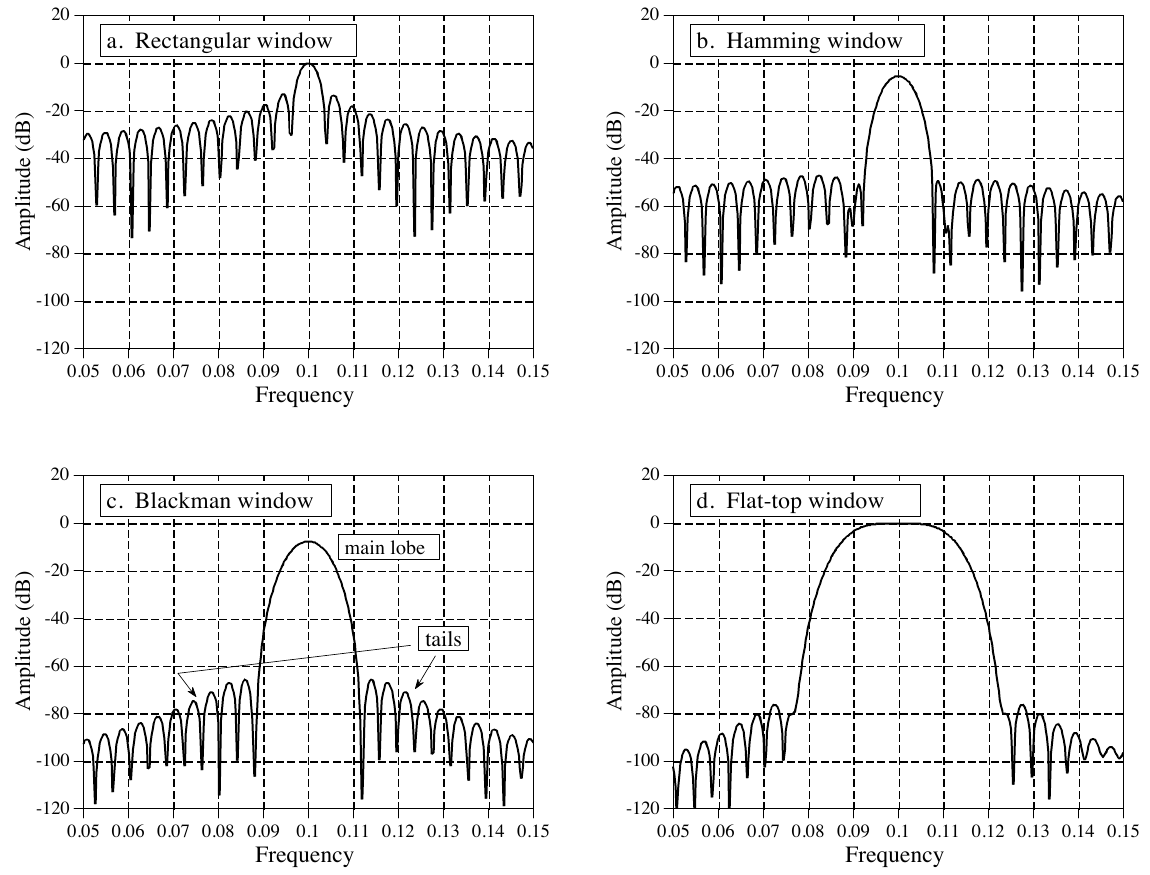
\includegraphics[width=0.958\linewidth,height=0.8\textheight,keepaspectratio]{assets/ch09/fig9-05.png}
\caption*{\textbf{图 9-5　用不同的窗时频谱峰的细节。}
频谱中的每个峰都是一个中央主瓣，四周是由旁瓣构成的尾巴。改变窗的形状，可以以主瓣变宽为代价降低旁瓣的幅度。矩形窗
(a) 的主瓣最窄，但旁瓣幅度最大。汉明窗 (b) 和布莱克曼窗 (c)
的旁瓣幅度较低，代价是主瓣较宽。平顶窗 (d)
用于必须精确测量峰的幅度的场合。这些曲线对应 255
点的窗；窗越长，峰按比例越窄。 （a. Rectangular window = 矩形窗；b.
Hamming window = 汉明窗；c.~Blackman window = 布莱克曼窗；d.~Flat-top
window = 平顶窗；main lobe = 主瓣，tails = 尾巴。Amplitude (dB) =
幅度（分贝），Frequency = 频率。）}
\end{figure}

这就引出了为了能在计算机中表示，需要对时域信号做的第二种修改：从信号中选取
N 个点。这 N
个点必须包含窗所确定的全部非零点，但也可以包含任意多个零。这样做的效果是对频谱的连续曲线进行采样。例如，如果
N 取 1024，频谱的连续曲线就在 0 到 0.5 之间被采样 513 次。如果 N
取得比窗长大得多，频域中的采样就会足够密，连续曲线的峰和谷都能在新频谱中保留下来。如果
N
取得和窗长一样，频谱中的采样较少，峰谷规则交替的图样就会变成不规则的尾巴，具体是什么样子取决于采样恰好落在哪里。这就解释了为什么图
9-4a 中的两个峰看起来不一样。图 9-4a 中的每个峰，都是对图 9-5a
中那条底层曲线的一次采样。尾巴有没有，取决于采样位置与峰、谷的相对关系。如果正弦波恰好与某个基函数相符，采样就恰好落在谷底，尾巴消失。如果正弦波位于两个基函数之间，采样就落在峰谷之间的某些位置，形成各种样子的尾巴。

这就引出了图 9-5d 所示的平顶窗(flat-top
window)。在某些应用中，频谱峰的幅度必须测得非常准。由于 DFT
的频谱是由采样构成的，没有什么能保证某个采样恰好落在峰顶。更可能的情况是，最近的那个采样稍稍偏离中心，得到的值比真实幅度低。解决办法是使用一种能让频谱峰顶部平坦的窗，确保总有一个或多个采样取到正确的峰值。如图
9-5d 所示，代价是主瓣非常宽，导致频率分辨率很差。

事实上，我们想要的平顶窗的形状，恰好和低通滤波器的滤波器核形状完全相同。后面的章节会讨论其中的理论原因；这里先给出这种技术的使用''菜谱''。第
16 章讨论一种叫加窗 sinc(windowed-sinc) 的低通滤波器。公式 16-4
描述了怎样生成它的滤波器核（我们要把它用作窗），图 16-4a
画出了这条曲线的典型形状。要用这个公式，需要知道两个参数的值：M 和
\(f_c\)。它们由下面的关系求出：\(M = N - 2\)，\(f_c = s/N\)，其中 N
是所用 DFT 的长度，s 是你希望峰的平坦部分上有几个采样（通常在 3 到 5
之间）。表 16-1
给出了计算这个滤波器核（也就是我们的窗）的程序，其中包含两个细微之处：归一化常数
K，以及怎样避免中心采样处除以零的错误。使用这种方法时要记住：时域中值为一的直流，会在频域中产生幅度为一的峰；但时域中幅度为一的正弦波，只会产生幅度为二分之一的频谱峰。（这在上一章的''合成：计算逆
DFT''一节讨论过。）

\section{系统的频率响应}

在时域中，用卷积来分析系统。在频域中也可以做类似的分析。利用傅里叶变换，每个输入信号都可以表示为一组余弦波，每个余弦波有确定的幅度和相移。同样，DFT
也可以把每个输出信号表示成类似的形式。这意味着任何线性系统都可以完全由它怎样改变通过它的余弦波的幅度和相位来描述。这些信息叫做系统的频率响应。由于冲激响应和频率响应都包含了关于系统的完整信息，两者之间必然一一对应。知道其中一个，就能算出另一个。冲激响应与频率响应之间的关系，是信号处理的基石之一：\textbf{系统的频率响应是其冲激响应的傅里叶变换。}图
9-6 展示了这些关系。

按照 DSP 的标准记法，冲激响应用小写变量，对应的频率响应用大写。由于 h{[}
{]} 是冲激响应的常用符号，频率响应就用 H{[}
{]}。系统在时域中用卷积描述，即
\(x[n] * h[n] = y[n]\)。在频域中，输入频谱乘以频率响应，得到输出频谱。写成公式：\(X[f] \times H[f] = Y[f]\)。也就是说，时域中的卷积对应频域中的乘法。

\begin{figure}[htbp]
\centering
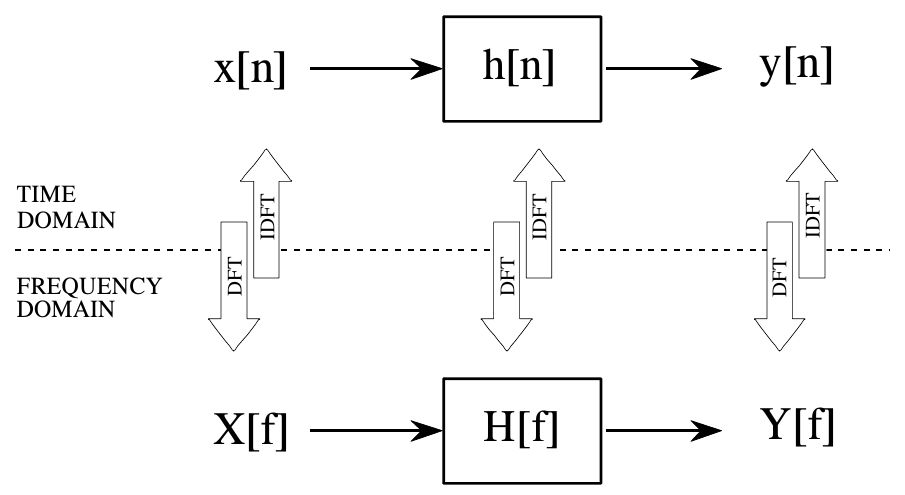
\includegraphics[width=0.754\linewidth,height=0.8\textheight,keepaspectratio]{assets/ch09/fig9-06.png}
\caption*{\textbf{图 9-6　比较系统在时域和频域中的运作。}
在时域中，输入信号与冲激响应卷积，得到输出信号，即
\(x[n] * h[n] = y[n]\)。在频域中，输入频谱乘以频率响应，得到输出频谱，即
\(X[f] \times H[f] = Y[f]\)。DFT 和逆 DFT 把两个域中的信号联系起来。
（TIME DOMAIN = 时域，FREQUENCY DOMAIN = 频域；DFT =
离散傅里叶变换，IDFT = 逆 DFT。）}
\end{figure}

图 9-7 是用 DFT 把系统的冲激响应转换成频率响应的一个例子。(a)
是系统的冲激响应。看这条曲线，你一点也看不出这个系统是做什么的。对这个冲激响应做
64 点 DFT，得到系统的频率响应，见
(b)。现在这个系统的作用就一目了然了：它让 0.2 到 0.3
之间的频率通过，挡住其他所有频率。这是一个带通滤波器(band-pass
filter)。也可以考察频率响应的相位，不过它更难解释，也没那么有意思。后面的章节会讨论它。

\begin{enumerate}
\def\labelenumi{(\alph{enumi})}
\setcounter{enumi}{1}
\tightlist
\item
  非常参差不齐，这是因为确定这条曲线的采样太少。在做 DFT
  之前给冲激响应补零，可以改善这种情况。例如，补零使冲激响应长 512
  个采样，如 (c) 所示，就得到 (d) 中分辨率更高的频率响应。
\end{enumerate}

\begin{figure}[htbp]
\centering
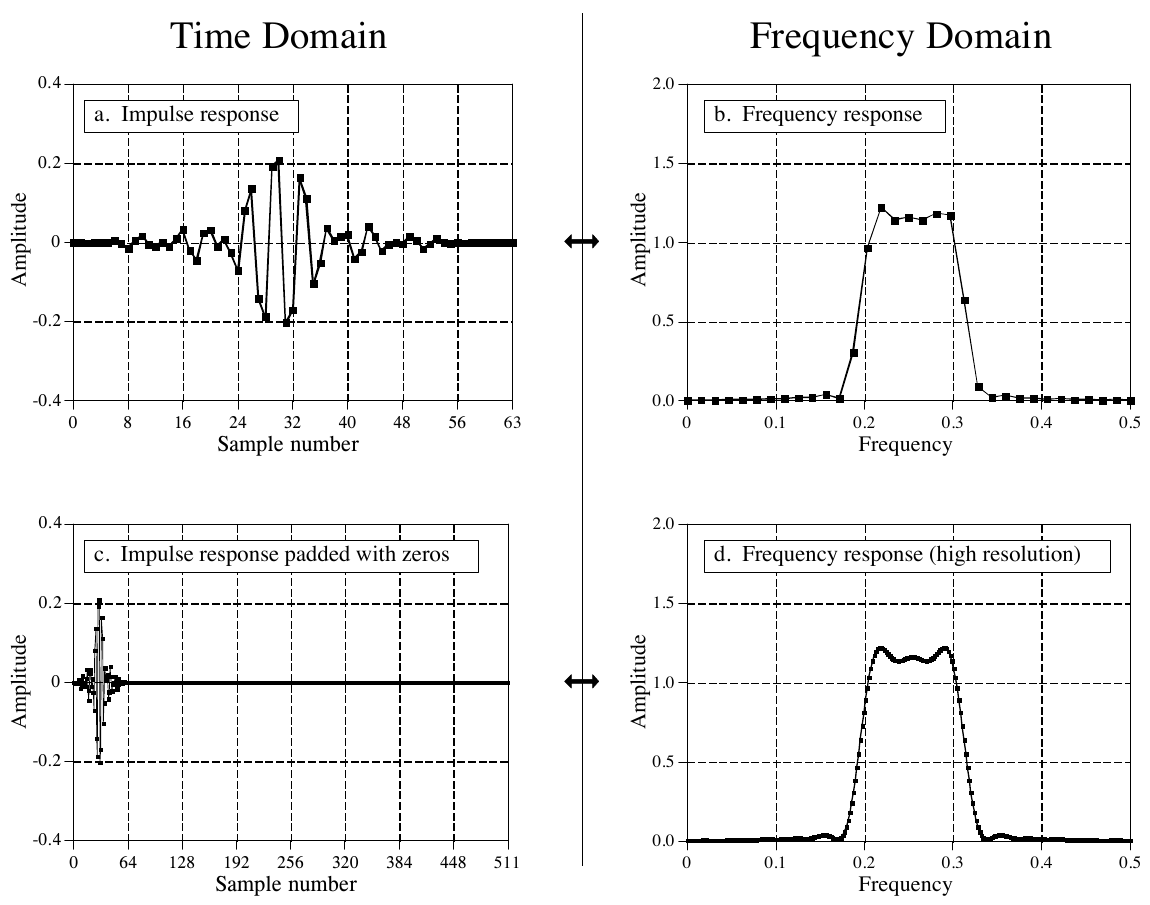
\includegraphics[width=0.958\linewidth,height=0.8\textheight,keepaspectratio]{assets/ch09/fig9-07.png}
\caption*{\textbf{图 9-7　由冲激响应求频率响应。} 利用 DFT，系统的冲激响应 (a)
可以变换成系统的频率响应 (b)。给冲激响应补零
(c)，可以在频率响应中得到更高的分辨率
(d)。本例只画了频率响应的幅度，相位的讨论推迟到下一章。 （Time Domain =
时域，Frequency Domain = 频域；a. Impulse response = 冲激响应；b.
Frequency response = 频率响应；c.~Impulse response padded with zeros =
补零后的冲激响应；d.~Frequency response (high resolution) =
频率响应（高分辨率）。Amplitude = 幅度，Sample number =
采样序号，Frequency = 频率。）}
\end{figure}

频率响应能得到多高的分辨率？答案是：无限高，只要你愿意给冲激响应补无限多个零。换句话说，除了
DFT
的长度，没有什么限制频率分辨率。这引出一个非常重要的概念：尽管冲激响应是离散信号，对应的频率响应却是连续的。对冲激响应做
N 点 DFT，得到这条连续曲线的 N/2 + 1 个采样。DFT
做得越长，分辨率越高，你对这条连续曲线长什么样的了解就越清楚。记住频率响应代表什么：余弦波通过系统时经历的幅度和相位变化。由于输入信号可以包含
0 到 0.5 之间的任何频率，系统的频率响应在这个范围内必须是一条连续曲线。

引入傅里叶变换家族的另一个成员------离散时间傅里叶变换（Discrete Time
Fourier Transform，DTFT），可以更好地理解这一点。考虑一个 N
个采样的信号通过 N 点 DFT，产生 N/2 + 1 个采样的频域。回忆上一章：DFT
把时域信号看作无限长、周期性的。也就是说，这 N
个点从负无穷到正无穷一遍又一遍地重复。现在考虑我们开始给时域信号补越来越多的零，以便在频域中得到越来越细的采样，会发生什么。补零使时域的周期变长，同时使频域的采样靠得更近。

现在把这推到极端：给时域信号补无限多个零。这在两个方面造成了不同的局面。第一，时域信号现在的周期无限长。换句话说，它变成了非周期信号。第二，频域的采样间距变得无限小。也就是说，它变成了连续信号。这就是
DTFT：把时域中离散的非周期信号，变成频域中一条连续曲线的过程。用数学的话说，系统的频率响应是对它的冲激响应做
DTFT 得到的。由于这在计算机里做不到，就用 DFT
来计算真实频率响应的一组采样。这就是你在计算机里做的（DFT）与你用数学公式做的（DTFT）之间的区别。

\section{通过频域做卷积}

假设你讨厌卷积。给你一个输入信号和一个冲激响应，要求出输出信号，你会怎么办？图
9-8
给出了一个答案：把两个信号变换到频域，相乘，再把结果变换回时域。这就把一次卷积换成了两次
DFT、一次乘法和一次逆
DFT。尽管中间步骤截然不同，输出和标准卷积算法完全相同。

有人讨厌卷积到愿意费这个周折吗？答案是有。避开卷积有两个原因。第一，卷积在数学上很难处理。例如，假设给你一个系统的冲激响应和它的输出信号，怎样算出输入信号是什么？这叫解卷积(deconvolution)，在时域里几乎无法理解。然而在频域里，解卷积可以用一次简单的除法------乘法的逆运算------来完成。只要傅里叶变换的复杂度低于卷积的复杂度，频域就有吸引力。这不是你更喜欢哪个的问题，而是你更不讨厌哪个的问题。

避开卷积的第二个原因是计算速度。例如，假设你设计了一个数字滤波器，它的核（冲激响应）有
512 个采样。在一台 200
MHz、使用浮点数的个人计算机上，用标准卷积算法，输出信号的每个采样大约需要一毫秒来计算。换句话说，系统的吞吐量只有每秒约
1000 个采样。这对高保真音频来说慢了 40 倍，对电视画质的视频来说慢了
10,000 倍！

标准卷积算法慢，是因为必须计算大量的乘法和加法。遗憾的是，仅仅用 DFT
把问题搬到频域里毫无帮助。计算 DFT
所需的运算量，和直接计算卷积一样多。1960 年代初快速傅里叶变换（Fast
Fourier Transform，FFT）的提出，使这个问题取得了突破。FFT 是一种快速计算
DFT 的巧妙算法。利用
FFT，通过频域相乘做卷积，可以比常规卷积快几百倍。要算好几个小时的问题，缩短到只要几分钟。这就是为什么人们对
FFT 和在频域中处理信号如此兴奋。FFT 将在第 12 章介绍，FFT 卷积的方法在第
18 章介绍。眼下先集中精力理解信号怎样通过频域相乘来卷积。

\begin{figure}[htbp]
\centering
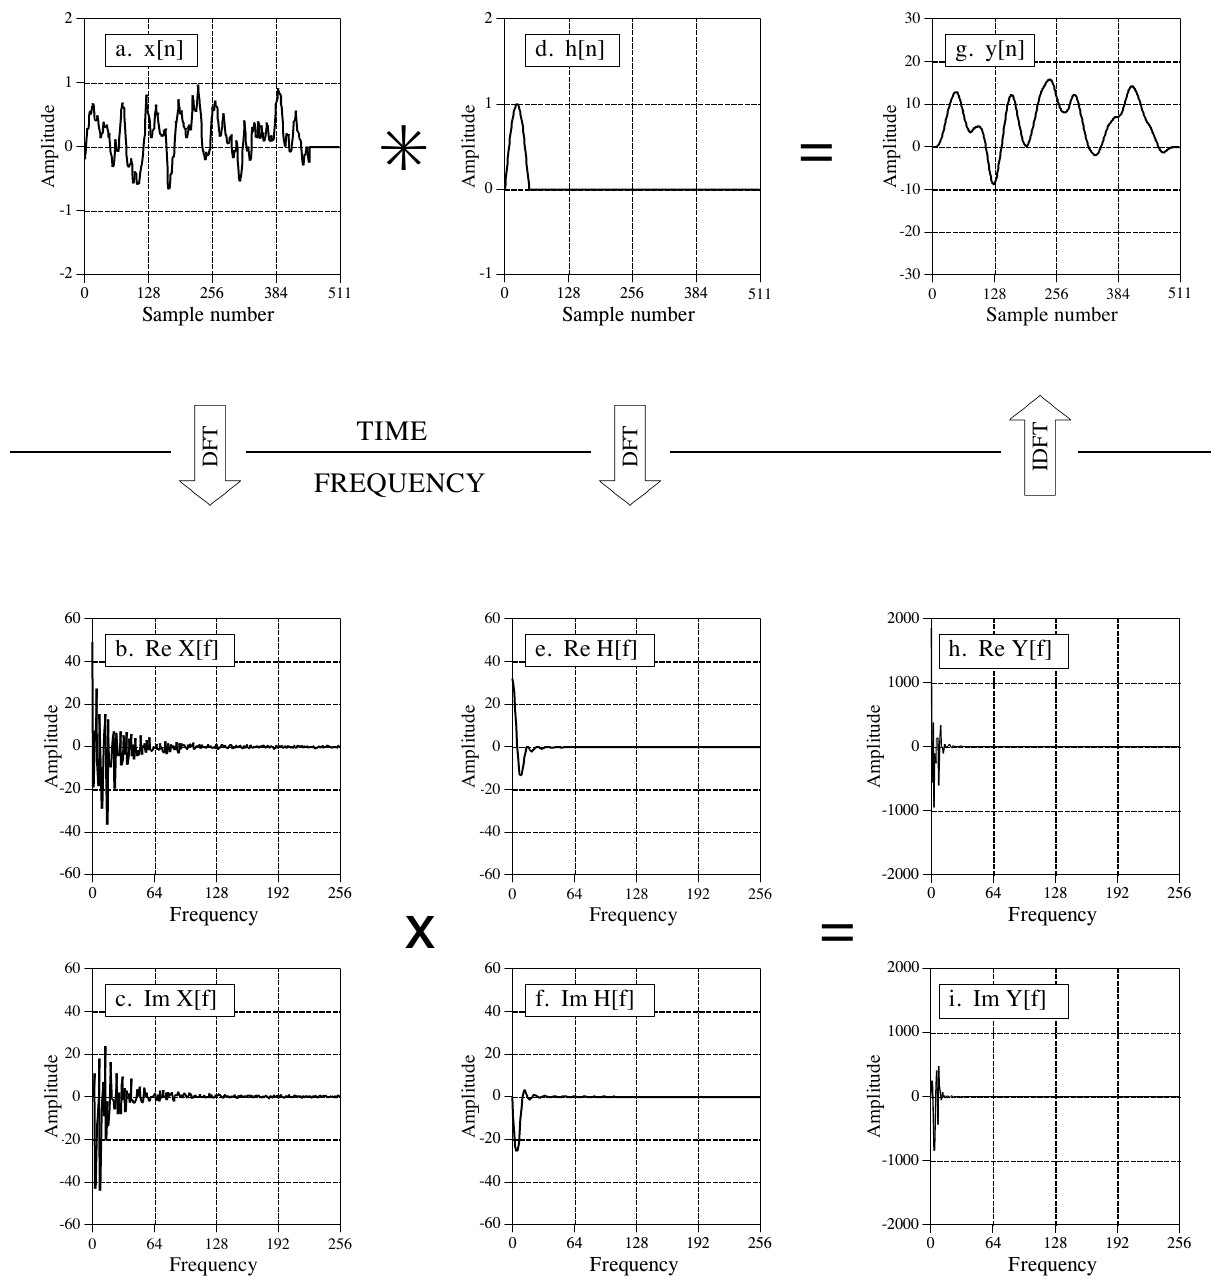
\includegraphics[width=1.000\linewidth,height=0.8\textheight,keepaspectratio]{assets/ch09/fig9-08.png}
\caption*{\textbf{图 9-8　频域卷积。} 在时域中，x{[}n{]} 与 h{[}n{]} 卷积得到
y{[}n{]}，如 (a)、(d)、(g) 所示。同样的过程也可以在频域中完成：用 DFT
求出输入信号的频谱 (b)、(c) 和系统的频率响应
(e)、(f)，把这两个频域信号相乘，得到输出信号的频谱 (h)、(i)，再用逆 DFT
求出输出信号 (g)。 （a. x{[}n{]}；d.~h{[}n{]}；g. y{[}n{]}；b. Re
X{[}f{]}；c.~Im X{[}f{]}；e. Re H{[}f{]}；f.~Im H{[}f{]}；h. Re
Y{[}f{]}；i. Im Y{[}f{]}。TIME = 时域，FREQUENCY = 频域；\dspsym{∗}
为卷积，x 为相乘。Amplitude = 幅度，Sample number = 采样序号，Frequency
= 频率。）}
\end{figure}

首先，需要定义一个频域信号怎样乘以另一个频域信号，即
\(X[f] \times H[f] = Y[f]\)
是什么意思。在极坐标形式下，幅度相乘：\(\mathrm{Mag}\,Y[f] = \mathrm{Mag}\,X[f] \times \mathrm{Mag}\,H[f]\)；相位相加：\(\mathrm{Phase}\,Y[f] = \mathrm{Phase}\,X[f] + \mathrm{Phase}\,H[f]\)。要理解这一点，可以设想一个具有某个幅度和相位的余弦波进入系统。同样，输出信号也是一个具有某个幅度和相位的余弦波。频率响应的极坐标形式，直接描述了这两个幅度之间以及两个相位之间的关系。

用直角坐标形式做频域乘法时，实部和虚部之间会有交叉项。例如，进入系统的正弦波在输出中可以同时产生余弦波和正弦波。用直角坐标记法做频域信号相乘：

\textbf{公式
9-1}　频域信号在直角坐标形式下的乘法：\(Y[f] = X[f] \times H[f]\)。

\[\mathrm{Re}\,Y[f] = \mathrm{Re}\,X[f]\,\mathrm{Re}\,H[f] - \mathrm{Im}\,X[f]\,\mathrm{Im}\,H[f]\]

\[\mathrm{Im}\,Y[f] = \mathrm{Im}\,X[f]\,\mathrm{Re}\,H[f] + \mathrm{Re}\,X[f]\,\mathrm{Im}\,H[f]\]

重点放在用极坐标记法理解乘法、理解余弦波通过系统的思路上。然后只需接受：同样的运算在直角坐标形式下进行，就会得到这些更复杂的式子。再比如，看看一个频域信号除以另一个频域信号。在极坐标形式下，频域信号的除法用乘法所用运算的逆运算来实现。要计算
\(H[f] = Y[f] / X[f]\)，就把幅度相除、相位相减，即
\(\mathrm{Mag}\,H[f] = \mathrm{Mag}\,Y[f] / \mathrm{Mag}\,X[f]\)，\(\mathrm{Phase}\,H[f] = \mathrm{Phase}\,Y[f] - \mathrm{Phase}\,X[f]\)。在直角坐标形式下则变成：

\textbf{公式 9-2}　频域信号在直角坐标形式下的除法，其中
\(H[f] = Y[f] / X[f]\)。

\[\mathrm{Re}\,H[f] = \frac{\mathrm{Re}\,Y[f]\,\mathrm{Re}\,X[f] + \mathrm{Im}\,Y[f]\,\mathrm{Im}\,X[f]}{\mathrm{Re}\,X[f]^2 + \mathrm{Im}\,X[f]^2}\]

\[\mathrm{Im}\,H[f] = \frac{\mathrm{Im}\,Y[f]\,\mathrm{Re}\,X[f] - \mathrm{Re}\,Y[f]\,\mathrm{Im}\,X[f]}{\mathrm{Re}\,X[f]^2 + \mathrm{Im}\,X[f]^2}\]

现在回到频域卷积。你可能已经注意到，我们在图 9-8 中稍微作了弊。记住，N
点信号与 M 点冲激响应卷积，得到 N + M − 1
点的输出信号。我们作弊的方式是：把输入信号的最后一部分全设成零，让输出有扩展的空间。具体来说，输入信号有
453 个非零采样，冲激响应有 60
个非零采样。这意味着两者的卷积能宽裕地放进提供的 512 个点里。

\begin{quote}
\textbf{译注：} 原文这里写的是''(a) contains 453 nonzero samples, and
(b) contains 60 nonzero samples \ldots{} the convolution of the two,
shown in (c)``，但说的是图 9-8，那张图里输入、冲激响应、输出分别是
(a)、(d)、(g)，不是
(a)、(b)、(c)。这里改为直接说''输入信号''\,``冲激响应''。453 + 60 − 1 =
512，恰好放满。
\end{quote}

现在考虑图 9-9 这种更一般的情况。输入信号 (a) 长 256 个点，冲激响应 (b)
有 51 个非零点。这使两个信号的卷积长 306 个采样，如 (c)
所示。问题是，如果用频域相乘来做这个卷积，输出信号只允许有 256
个采样。换句话说，用 256 点 DFT 把 (a) 和 (b) 搬到频域，相乘之后，再用
256 点逆 DFT 求出输出信号。怎样把正确信号的 306 个值塞进频域算法提供的
256 个点里？答案是：塞不进去！这 256
个点最终成了正确信号的一个失真版本。这个过程叫循环卷积(circular
convolution)。它之所以重要，是因为你要避开它。

\begin{figure}[htbp]
\centering
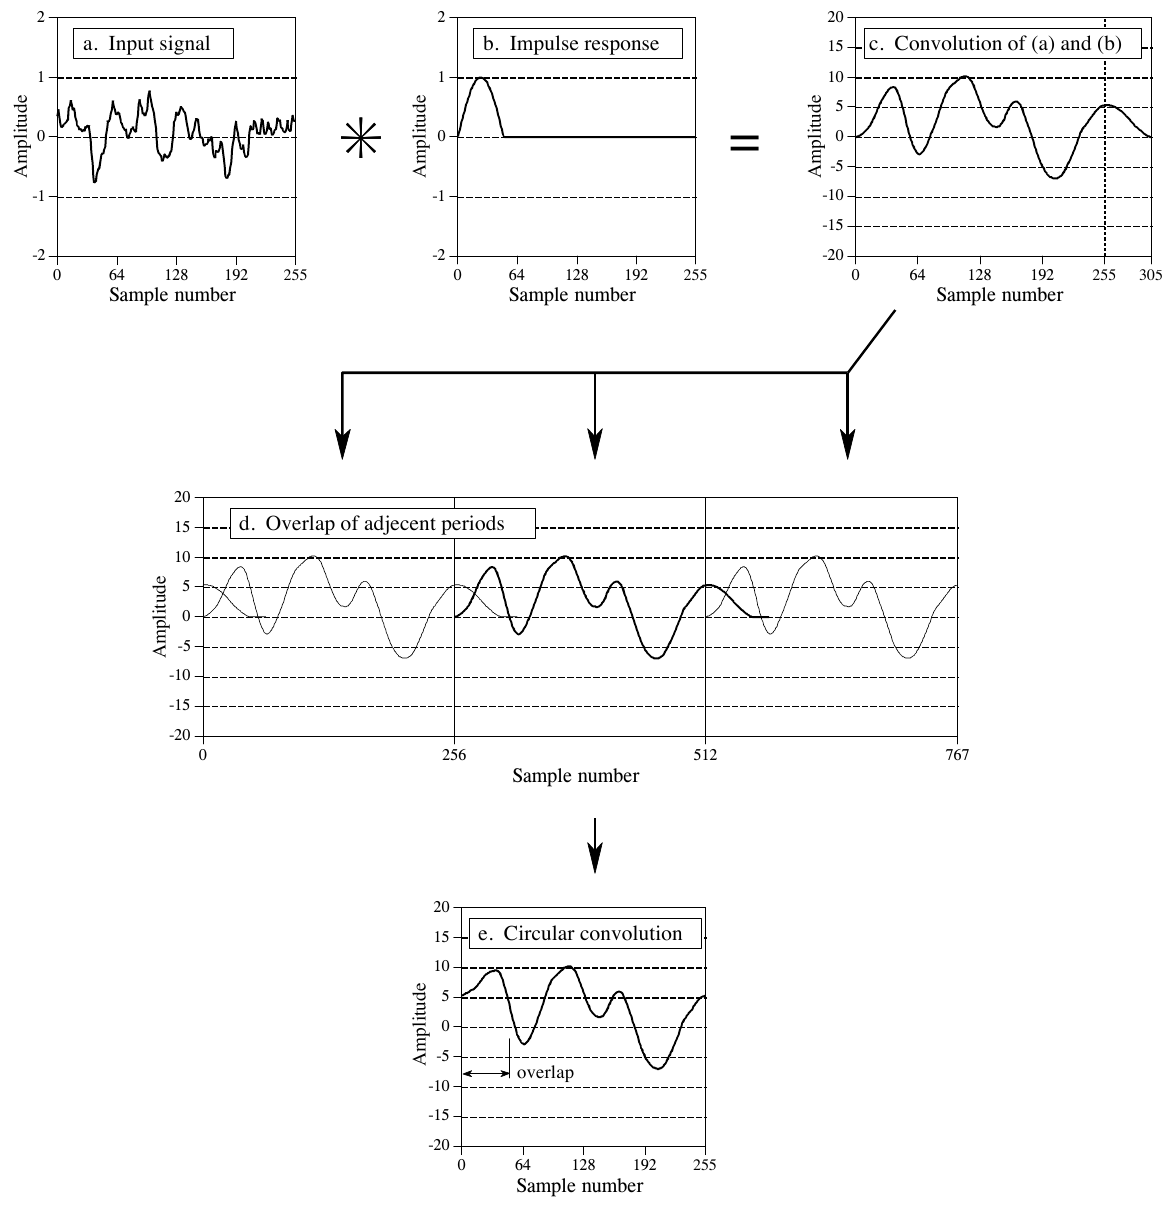
\includegraphics[width=0.971\linewidth,height=0.8\textheight,keepaspectratio]{assets/ch09/fig9-09.png}
\caption*{\textbf{图 9-9　循环卷积。} 256 个采样的信号 (a) 与 51 个采样的冲激响应
(b) 卷积，得到 306 个采样的信号 (c)。如果用 256 点 DFT
在频域中做这个卷积，正确卷积结果的 306 个点放不进提供的 256 个采样里。如
(d) 所示，输出信号的第 256 到 305
个采样被推进右边的下一个周期，与下一周期信号的开头相加。(e)
是所得信号的一个周期。 （a. Input signal = 输入信号；b. Impulse response
= 冲激响应；c.~Convolution of (a) and (b) = (a) 与 (b)
的卷积；d.~Overlap of adjecent periods = 相邻周期的重叠（adjecent
为原书拼写错误，应为 adjacent）；e. Circular convolution =
循环卷积；overlap = 重叠部分。Amplitude = 幅度，Sample number =
采样序号。）}
\end{figure}

要理解循环卷积，记住 N 点 DFT 把时域看作一个无限长的周期信号，每个周期 N
个采样。图 (d) 画出了本例中 DFT 眼里输出信号的三个周期。由于 N =
256，每个周期有 256 个点：0～255、256～511 和 512～767。频域卷积试图把
(c) 中 306 点的正确输出信号放进每个 256 点的周期里。结果有 49
个采样被推进右边相邻的周期，与本来就在那里的采样重叠。这些重叠部分相加，使每个周期都呈现为
(e) 的样子，也就是循环卷积。

\begin{quote}
\textbf{译注：} 按图注，被推出去的是第 256 到 305 个采样，共 306 − 256 =
50 个，正文写的 49 个应为 50 个。
\end{quote}

一旦理解了循环卷积的本质，避开它就很容易了。只要给参与卷积的每个信号补足够多的零，让输出信号有空间容纳正确卷积结果的
N + M − 1 个点。例如，可以把 (a) 和 (b) 中的信号补零到 512 点长，然后用
512 点 DFT。做完频域卷积后，输出信号由 306 个非零采样加上 206
个值为零的采样组成。第 18 章会详细讲解这个过程。

为什么叫循环卷积？回头看图 9-9d，考察中间那个周期，即第 256 到 511
个采样。由于所有周期都一样，从这个周期右边流出去的那部分信号，和从左边流进这个周期的那部分是一样的。如果只考虑单个周期，比如
(e)，看起来信号的右边不知怎么和左边连在了一起。想象一条咬住自己尾巴的蛇：第
255 个采样紧挨着第 0 个采样，就像第 100 个采样紧挨着第 101
个采样一样。信号的一部分从右边出去时，会神奇地从左边重新出现。换句话说，N
点时域的行为就像它是一个圆环。

上一章我们提出过一个问题：把 DFT 的时域看作 N 个点，还是看作周期为 N
的无限长周期信号，真的有区别吗？循环卷积就是一个有区别的例子。如果把时域信号理解为周期性的，循环卷积中遇到的失真就可以简单地解释为信号从一个周期扩展到了下一个周期。相比之下，如果只考虑时域的
N
个点，就会得出一个相当离奇的结论：频域卷积的作用就好像时域不知怎么卷成了一个圆环，第
0 个采样紧挨着第 N−1 个采样。

% !TEX root = ../main.tex
% 本文件由 build-tex.sh 从 10-DSP指南-第10章中译.md 生成，改内容请改 md 后重新生成

\chapter{傅里叶变换的性质}\label{ch-10}

时域和频域是表示信号的两种可以互换的方式。傅里叶变换(Fourier
transform)就是这两种表示之间的数学关系。如果信号在一个域里被修改了，它在另一个域里也会随之改变，只是改变的方式通常不一样。例如，上一章说明了：时域信号做卷积，结果是它们的频谱相乘。其他数学运算，比如相加、缩放和平移，在另一个域里也都有对应的运算。这些关系叫做傅里叶变换的性质(properties
of the Fourier
transform)，讲的是一个域里的数学变化会在另一个域里引起怎样的数学变化。

\section{傅里叶变换的线性}

傅里叶变换是线性的，也就是说，它具有齐次性(homogeneity)和可加性(additivity)。傅里叶变换家族的全部四个成员（傅里叶变换、傅里叶级数、DFT
和 DTFT）都是如此。

图 10-1 举例说明齐次性是傅里叶变换的一个性质。(a)
是一个任意的时域信号，(b) 是它对应的频谱。我们分别把这两个信号叫做 x{[}
{]} 和 X{[}
{]}。齐次性的意思是：一个域里的幅度变化，会在另一个域里产生同样的幅度变化。这在直觉上应该说得通：时域波形的幅度变了，组成这个波形的正弦波和余弦波的幅度也必然变同样的倍数。

写成数学语言：如果 x{[} {]} 和 X{[} {]} 是一对傅里叶变换对(Fourier
transform pair)，那么对任意常数 k，k x{[} {]} 和 k X{[} {]}
也是一对傅里叶变换对。如果频域用直角坐标表示，k X{[} {]}
的意思是实部和虚部都乘以 k；如果频域用极坐标表示，k X{[} {]}
的意思是幅度乘以 k，相位保持不变。

\begin{figure}[htbp]
\centering
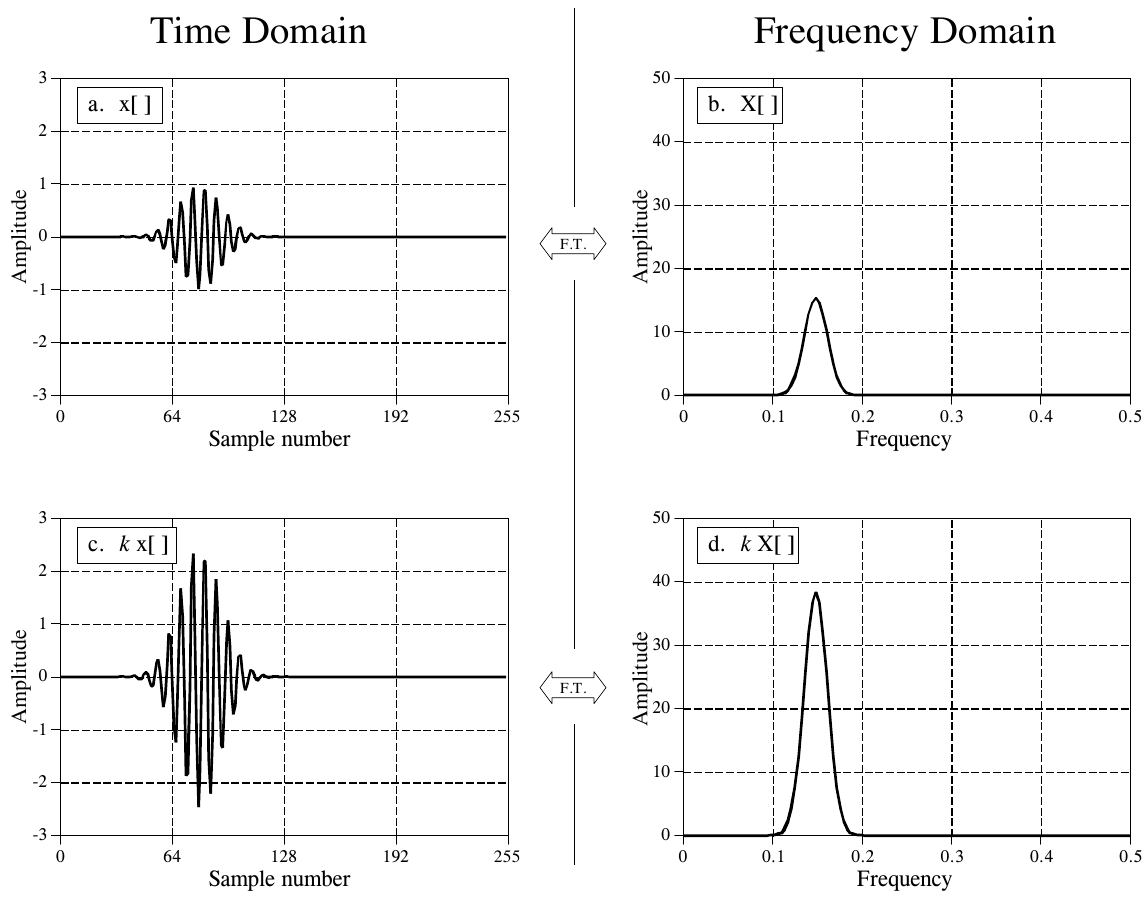
\includegraphics[width=0.954\linewidth,height=0.8\textheight,keepaspectratio]{assets/ch10/fig10-01.png}
\caption*{\textbf{图 10-1　傅里叶变换的齐次性。}
一个域里的幅度改变多少，另一个域里的幅度也改变同样多。换句话说，一个域里的缩放对应另一个域里的缩放。
（Time Domain = 时域，Frequency Domain = 频域；a. x{[} {]}，b. X{[}
{]}，c.~k x{[} {]}，d.~k X{[} {]}；中间的 F.T. = 傅里叶变换。Amplitude =
幅度，Sample number = 采样序号，Frequency = 频率。）}
\end{figure}

傅里叶变换的可加性是指：一个域里的相加对应另一个域里的相加。图 10-2
是一个例子。图中 (a) 和 (b) 是两个时域信号，分别叫 x₁{[} {]} 和 x₂{[}
{]}。把它们相加，得到第三个时域信号 x₃{[} {]}，如 (c)
所示。这三个信号每一个的频谱都由实部和虚部组成，见 (d) 到
(i)。由于两个时域信号相加得到第三个时域信号，两个对应的频谱也相加得到第三个频谱。在直角坐标表示下，频谱相加就是实部加实部、虚部加虚部。如果
\(x_1[n] + x_2[n] = x_3[n]\)，那么
\(\mathrm{Re}\,X_1[f] + \mathrm{Re}\,X_2[f] = \mathrm{Re}\,X_3[f]\)，并且
\(\mathrm{Im}\,X_1[f] + \mathrm{Im}\,X_2[f] = \mathrm{Im}\,X_3[f]\)。可以从余弦波和正弦波的角度来想：所有余弦波相加（实部），所有正弦波相加（虚部），两者之间互不干扰。

\begin{figure}[htbp]
\centering
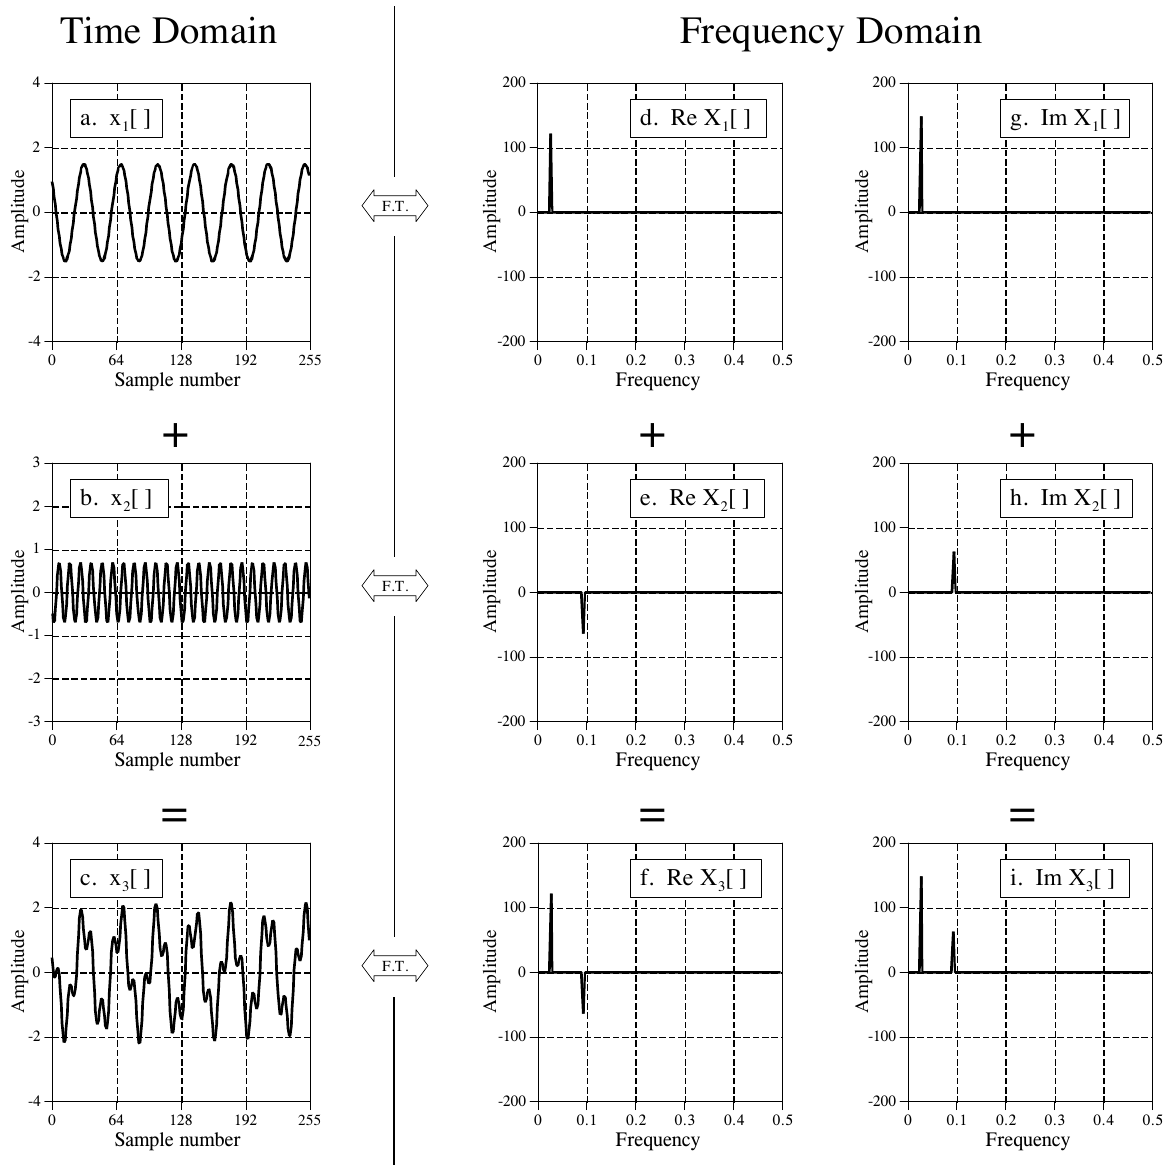
\includegraphics[width=0.971\linewidth,height=0.8\textheight,keepaspectratio]{assets/ch10/fig10-02.png}
\caption*{\textbf{图 10-2　傅里叶变换的可加性。}
在一个域里把两个或更多信号相加，另一个域里对应的信号也随之相加。本图中，(a)
和 (b) 两个时域信号相加得到 (c)，结果是频谱对应的实部和虚部分别相加。
（Time Domain = 时域，Frequency Domain = 频域；a～c 为 x₁{[} {]}、x₂{[}
{]}、x₃{[} {]}，d～f 为三者的实部 Re X{[} {]}，g～i 为三者的虚部 Im X{[}
{]}。F.T. = 傅里叶变换。Amplitude = 幅度，Sample number =
采样序号，Frequency = 频率。）}
\end{figure}

极坐标形式的频谱不能直接相加，必须先转成直角坐标，相加后再转回极坐标。这一点也可以从正弦波的行为来理解。设想把两个频率相同、但幅度（A₁
和 A₂）和相位（φ₁ 和 φ₂）不同的正弦波相加。如果两个相位恰好相同（φ₁ =
φ₂），相加时幅度相加（A₁ + A₂）。但如果两个相位恰好相反（φ₁ =
−φ₂），相加时幅度相减（A₁ −
A₂）。要点是：正弦波（或频谱）处于极坐标形式时，不能简单地把幅度和相位分别相加。

\begin{quote}
\textbf{译注：} ``两个相位恰好相反''严格说应是相差 π（φ₁ = φ₂ ±
π），这时两个正弦波反相，幅度才相减；原书写的 φ₁ = −φ₂ 只在 φ₂ = ±π/2
时才成立。这里按原书意思理解即可。
\end{quote}

傅里叶变换虽然是线性的，但它不具备平移不变性(shift
invariance)。换句话说，时域里的平移并不对应频域里的平移。这是下一节的主题。

\section{相位的特性}

写成数学语言：如果
\(x[n] \leftrightarrow \mathrm{Mag}\,X[f]\ \&\ \mathrm{Phase}\,X[f]\)，那么时域平移的结果是：\(x[n+s] \leftrightarrow \mathrm{Mag}\,X[f]\ \&\ \mathrm{Phase}\,X[f] + 2\pi s f\)（其中
f 用采样率的分数表示，范围是 0 到 0.5）。用文字说，时域平移 s
个采样，幅度不变，但相位加上一个线性项 2πsf。我们来看一个例子。

图 10-3
展示了时域波形向左或向右平移时相位受到的影响。图中没有画幅度，因为它没什么可看的：时域平移不改变幅度。在
(a) 到 (d) 中，波形逐步平移，从峰值位于第 128 个采样，变成峰值位于第 0
个采样。这一组图考虑到了 DFT
把时域看作环形的：波形从右边出去的部分，会从左边重新出现。

图 10-3 中的时域波形关于一条竖轴对称，也就是左右两边互为镜像。第 7
章讲过，具有这种对称性的信号叫线性相位(linear
phase)信号，因为它们频谱的相位是一条直线。同样，没有这种左右对称性的信号叫非线性相位(nonlinear
phase)信号，它们的相位不是直线。(e) 到 (h) 是 (a) 到 (d)
中各信号的相位。如第 7
章所述，这些相位都已展开(unwrapped)，所以不会出现为了把值保持在 π 到 −π
之间而产生的跳变。

时域波形向右平移时，相位仍是一条直线，但斜率减小；时域向左平移时，斜率增大。这是本节你需要记住的主要性质：时域里的平移，对应相位斜率的改变。

\begin{enumerate}
\def\labelenumi{(\alph{enumi})}
\setcounter{enumi}{1}
\tightlist
\item
  和 (f) 展示了一个特殊情形：相位完全为零。这发生在时域信号关于第 0
  个采样对称的时候。乍一看，(b)
  里的这种对称可能不明显，它看起来好像是关于第 256 个采样（即
  N/2）对称。记住，DFT 把时域看作环形的，第 0 个采样本来就和第 N−1
  个采样连在一起。任何关于第 0 个采样对称的信号，也必然关于第 N/2
  个采样对称，反之亦然。如果使用傅里叶变换家族中不把时域看作周期的成员（比如
  DTFT），则必须关于第 0 个采样对称才能得到零相位。
\end{enumerate}

\begin{figure}[htbp]
\centering
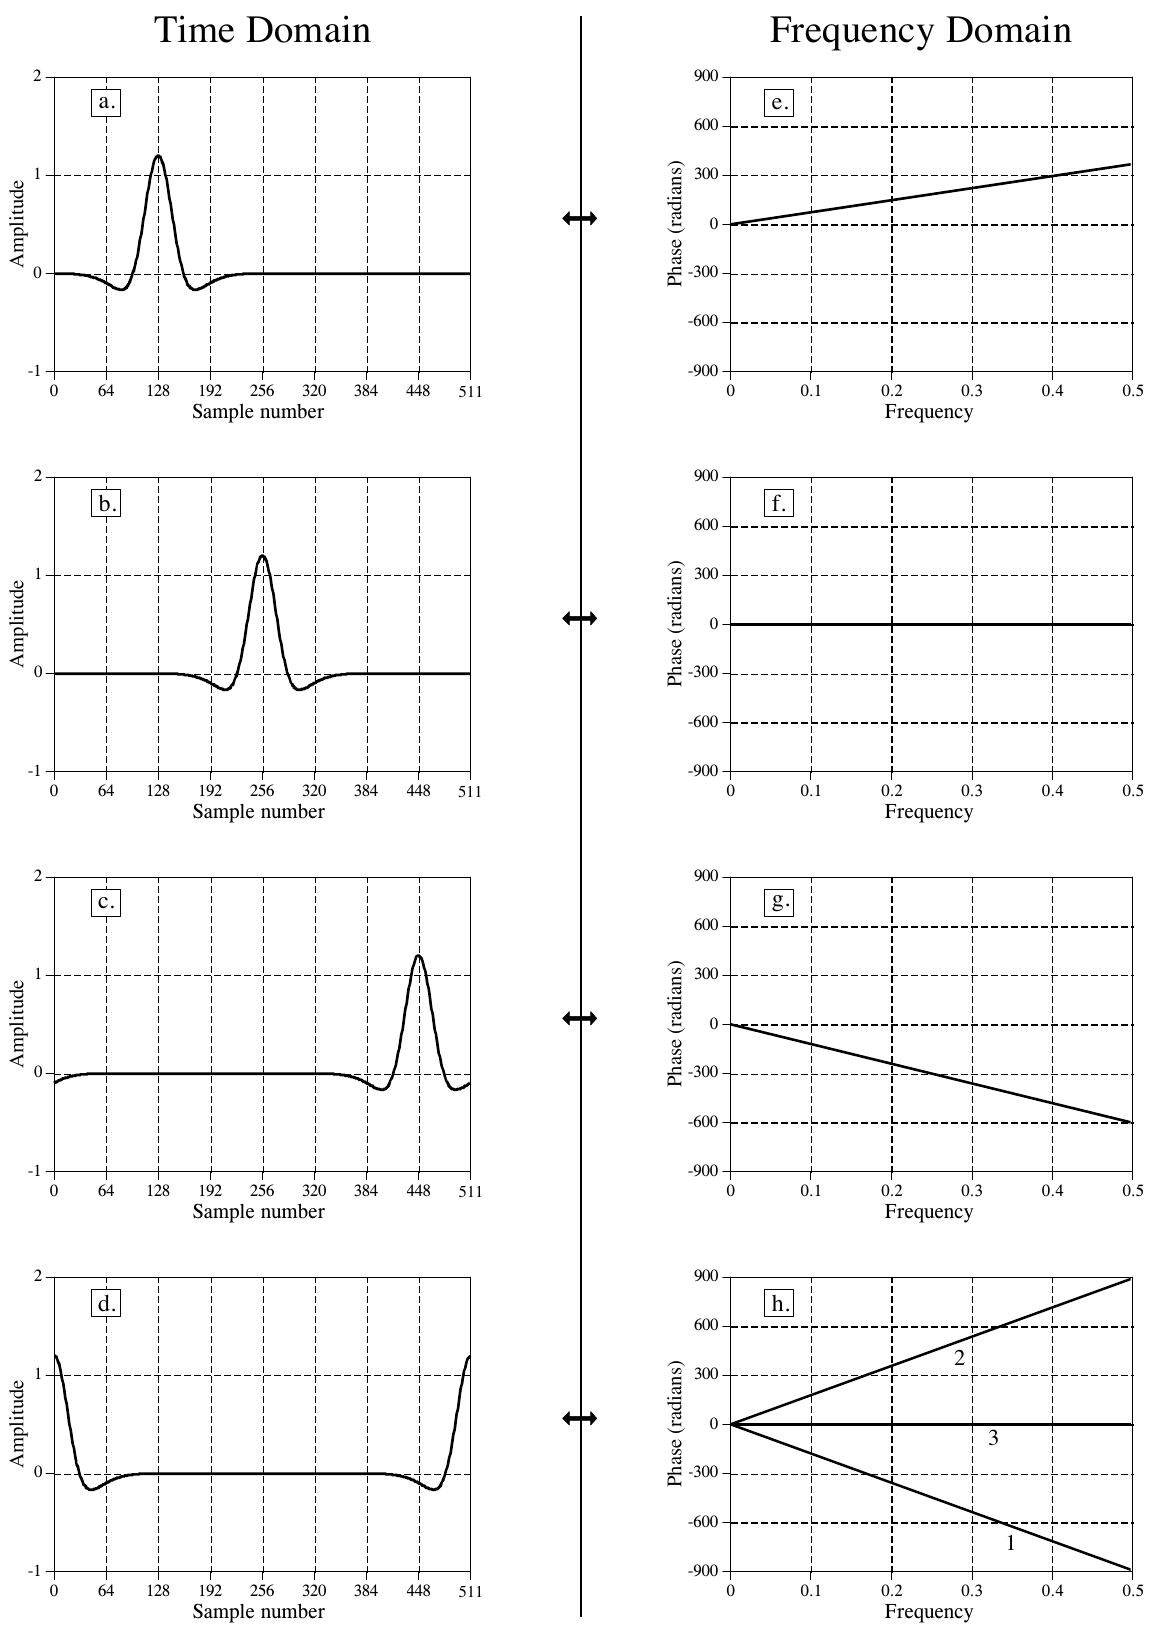
\includegraphics[width=0.958\linewidth,height=0.8\textheight,keepaspectratio]{assets/ch10/fig10-03.png}
\caption*{\textbf{图 10-3　时域平移引起的相位变化。} （Time Domain =
时域，Frequency Domain = 频域；左列 a～d 为时域波形，右列 e～h
为对应的相位。(h) 中的 1、2、3 是正文讨论的三条相位线。Amplitude =
幅度，Phase (radians) = 相位（弧度），Sample number =
采样序号，Frequency = 频率。）}
\end{figure}

\begin{enumerate}
\def\labelenumi{(\alph{enumi})}
\setcounter{enumi}{3}
\tightlist
\item
  和 (h) 呈现了一个谜题。首先，设想 (d) 是把 (c)
  中的波形再往右多移一点得到的。这意味着 (h) 中的相位斜率应该比 (g)
  更负一点，如第 1 条线所示。然后，设想 (d) 是从 (a)
  开始向左平移得到的。这时相位的斜率应该比 (e) 更正一点，如第 2
  条线所示。最后，注意 (d) 关于第 N/2 个采样对称，因此应该是零相位，如第
  3 条线所示。这三个相位哪个对？都对，取决于（第 8 章讨论过的）π 和 2π
  相位多值性(phase ambiguity)怎样取舍。例如，第 2 条线上的每个采样，与第
  1 条线上对应采样都相差 2π 的整数倍，所以两者相等。要把第 3 条线和第
  1、2 条线联系起来，还得考虑 π 的多值性。
\end{enumerate}

要理解相位为什么这样变化，设想把一个波形向右平移一个采样。这意味着组成这个波形的所有正弦波也都必须向右平移一个采样。图
10-4 画出了可能组成这个波形的两个正弦波。(a)
中正弦波的频率很低，平移一个采样只是一整个周期中很小的一部分。(b)
中正弦波的频率是采样率的一半，这是采样数据中能存在的最高频率。在这个频率上，平移一个采样相当于整整半个周期，即
π
弧度。也就是说，把平移量用相位变化来表示时，它与被平移的正弦波的频率成正比。

例如，考虑一个关于第 0 个采样对称、因而相位为零的波形。图 10-5a
展示了这个信号向左或向右平移时相位怎样变化。在最高频率（采样率的一半）处，每向左平移一个采样，相位增加
π；每向右平移一个采样，相位减少
π。在零频率处没有相移，中间的所有频率沿一条直线分布。

\begin{figure}[htbp]
\centering
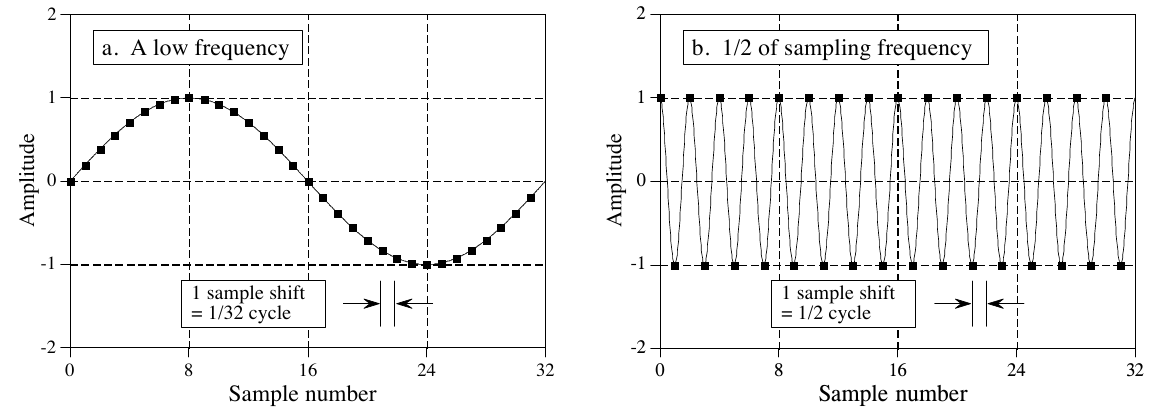
\includegraphics[width=0.958\linewidth,height=0.8\textheight,keepaspectratio]{assets/ch10/fig10-04.png}
\caption*{\textbf{图 10-4　采样与相位之间的关系。} (a) 和 (b)
分别是低频和高频的正弦波。在 (a) 中，平移一个采样等于 1/32 个周期；在
(b) 中，平移一个采样等于 1/2
个周期。这就是为什么波形平移时，高频处的相位变化比低频处大。 （a. A low
frequency = 一个低频；b. 1/2 of sampling frequency = 采样频率的
1/2。图中方框：1 sample shift = 1/32 cycle（或 1/2 cycle）= 平移 1
个采样 = 1/32（或 1/2）个周期。Amplitude = 幅度，Sample number =
采样序号。）}
\end{figure}

\begin{figure}[htbp]
\centering
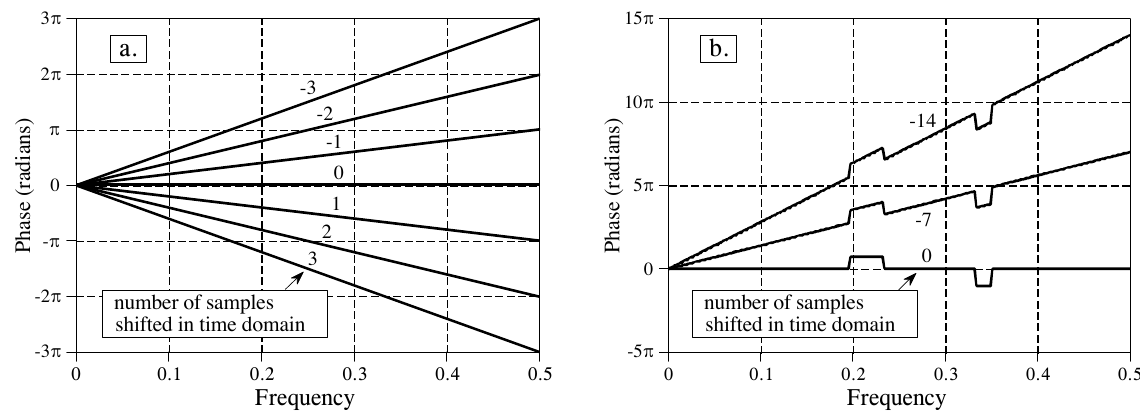
\includegraphics[width=0.950\linewidth,height=0.8\textheight,keepaspectratio]{assets/ch10/fig10-05.png}
\caption*{\textbf{图 10-5　时域平移产生的相位。}
时域信号每向正方向（即向右）平移一个采样，频率 0.5 处的相位减少 π
弧度；每向负方向（即向左）平移一个采样，频率 0.5 处的相位增加 π
弧度。(a) 展示的是线性相位（一条直线）的情形，(b)
是一个非线性相位的例子。 （各直线旁的数字是时域平移的采样数，方框 number
of samples shifted in time domain = 时域中平移的采样数。Phase (radians)
= 相位（弧度），Frequency = 频率。）}
\end{figure}

到目前为止我们用的例子都是线性相位的。图 10-5b
说明非线性相位信号对平移的反应也一样。本例中，非线性相位是一条直线加上两个矩形脉冲。时域平移时，这些非线性特征只是叠加在不断变化的斜率上。

时域波形平移时，实部和虚部会怎样？回想一下，直角坐标表示的频域信号对人来说几乎无法理解。实部和虚部通常看起来像毫无规律的随机振荡。时域信号一平移，实部和虚部那些弯弯曲曲的图案会振荡得更厉害，更难解读。别浪费时间去理解这些信号，或者它们怎样随时域平移而变化。

图 10-6
是一个有趣的演示，说明哪些信息包含在相位里，哪些信息包含在幅度里。(a)
中的波形有两个非常明显的特征：第 55 个采样处的上升沿和第 110
个采样处的下降沿。当信息编码在波形形状里时，边沿非常重要。边沿指明某件事发生的时刻，把它左边的东西和右边的东西分开。这是最纯粹的时域编码信息。演示开始时，先对
(a) 中的信号做 DFT，并把频谱转成极坐标表示。要得到 (b)
中的信号，把相位换成 −π 到 π 之间的随机数，再用逆 DFT
重建时域波形。换句话说，(b) 只基于幅度中包含的信息。同样，(c) 是在使用逆
DFT 之前，把幅度换成很小的随机数得到的。这使得 (c)
的重建只基于相位中包含的信息。

\begin{figure}[htbp]
\centering
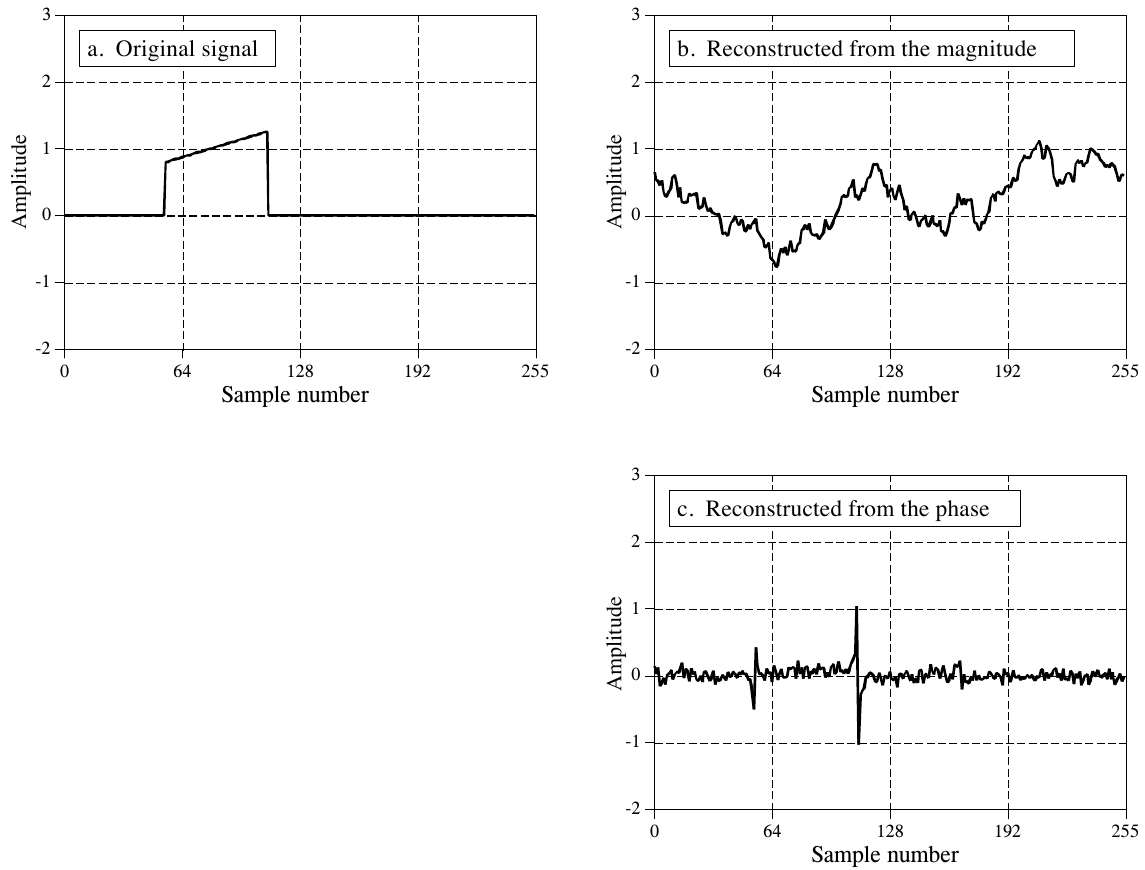
\includegraphics[width=0.954\linewidth,height=0.8\textheight,keepaspectratio]{assets/ch10/fig10-06.png}
\caption*{\textbf{图 10-6　相位中包含的信息。} (a) 是一个脉冲状的波形。(b)
的做法是：对 (a) 做 DFT，把相位换成随机数，再做逆 DFT。(c) 的做法是：对
(a) 做 DFT，把幅度换成随机数，再做逆 DFT。边沿的位置在 (c)
中保留下来了，在 (b)
中却没有。这说明相位包含了时域信号中事件发生位置的信息。 （a. Original
signal = 原信号；b. Reconstructed from the magnitude =
由幅度重建；c.~Reconstructed from the phase = 由相位重建。Amplitude =
幅度，Sample number =
采样序号。原书图注排在左下空白处，裁图时已去掉，译文见上。）}
\end{figure}

结果如何？边沿的位置在 (c) 中清清楚楚，在 (b)
中却完全消失了。这是因为，边沿是许多正弦波在同一位置一起上升形成的，只有当它们的相位相互配合时才可能做到。简而言之，时域波形形状的大部分信息包含在相位中，而不是幅度中。与此形成对比的是信息编码在频域中的信号，比如音频信号。对这类信号，幅度最重要，相位只起次要作用。后面的章节会看到，这种认识为设计滤波器和其他信号处理方法提供了思路。理解信息在信号中是怎样表示的，永远是成功做好
DSP 的第一步。

为什么左右对称对应零（或线性）相位？图 10-7
给出了答案。这样的信号可以分解成左半部分和右半部分，如 (a)、(b)、(c)
所示。位于对称中心（本例中是零点）的采样平均分给左右两半，使两边恰好互为镜像。这两半的幅度完全相同，如
(e) 和 (f) 所示；相位则符号相反，如 (h) 和 (i)
所示。由此得出两个重要概念。第一，每个左右对称的信号都具有线性相位，因为左半部分的非线性相位恰好抵消了右半部分的非线性相位。

\begin{figure}[htbp]
\centering
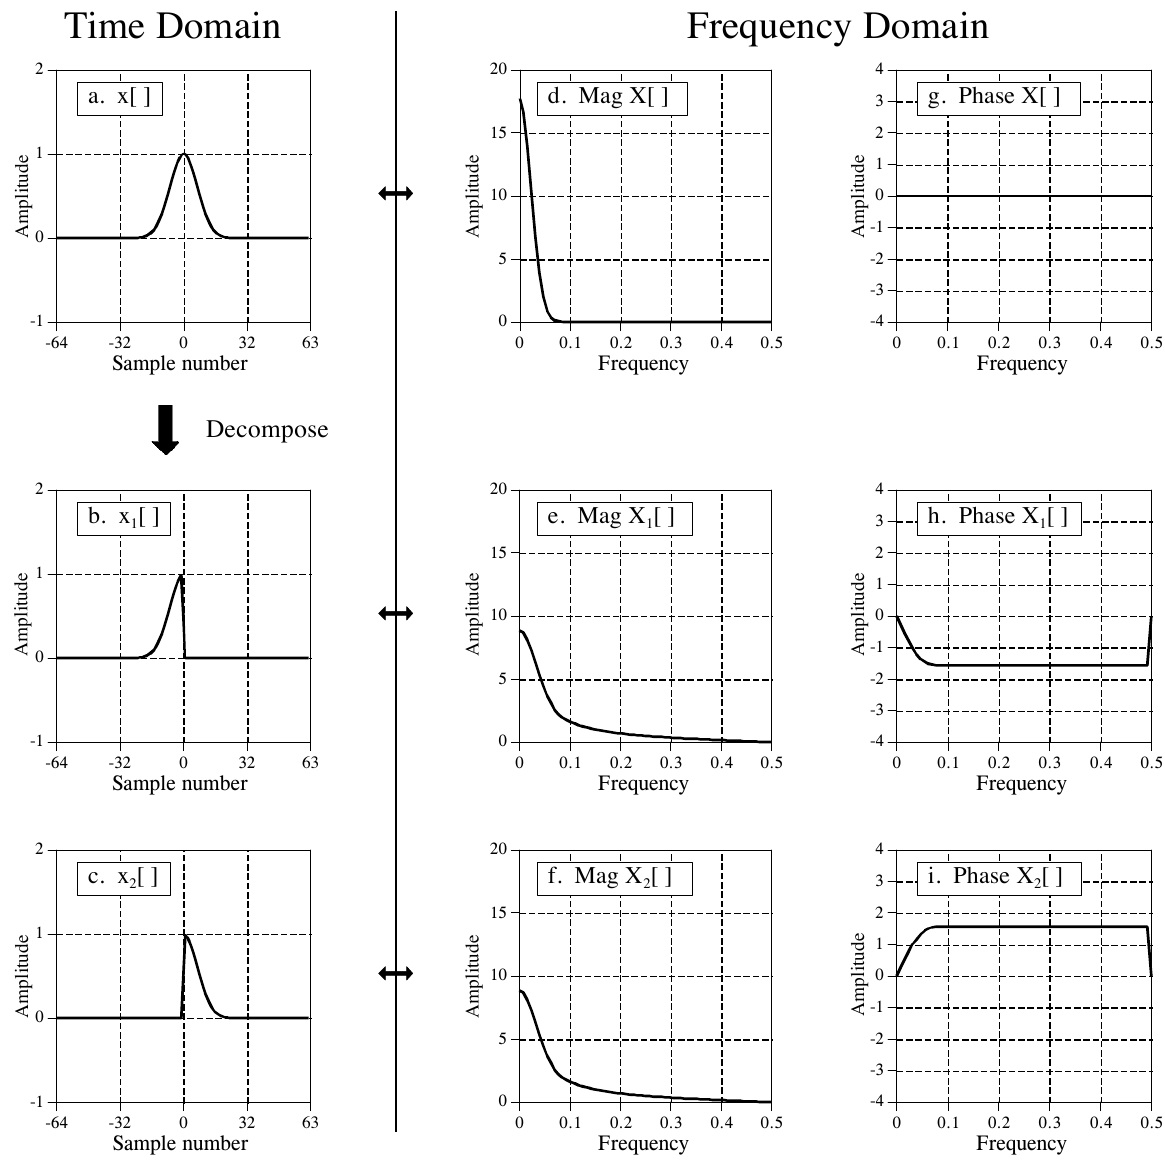
\includegraphics[width=0.971\linewidth,height=0.8\textheight,keepaspectratio]{assets/ch10/fig10-07.png}
\caption*{\textbf{图 10-7　左右对称的相位特性。} 一个左右对称的信号
(a)，可以分解成左半部分 (b) 和右半部分 (c)。两半的幅度完全相同，见 (e)
和 (f)；相位则互为相反数，见 (h) 和 (i)。 （Time Domain =
时域，Frequency Domain = 频域，Decompose = 分解；a～c 为 x{[} {]}、x₁{[}
{]}、x₂{[} {]}，d～f 为它们的幅度 Mag，g～i 为它们的相位
Phase。Amplitude = 幅度，Sample number = 采样序号，Frequency = 频率。）}
\end{figure}

\begin{quote}
\textbf{译注：} 原书图注写作''分解成右半部分 (b) 和左半部分
(c)``，与图不符：图中 (b) x₁{[} {]} 只在负序号处有值，是左半部分；(c)
x₂{[} {]} 是右半部分。正文的说法（左半、右半依次对应
(b)、(c)）是对的，译文按图改正。另外 (g)～(i) 的纵轴标的是
Amplitude，实际画的是相位（弧度）。
\end{quote}

第二，设想把 (b) 翻转成
(c)。时域里的这种左右翻转对幅度没有任何影响，但会把相位中每个点的符号都改变。同样，改变相位的符号，就会把时域信号左右翻转。如果信号是连续的，翻转是围绕零点进行的；如果信号是离散的，翻转同时围绕第
0 个采样和第 N/2 个采样进行。

改变相位符号是一种很常用的操作，因此有它自己的名称和符号。名称叫复共轭(complex
conjugation)，记法是在变量的右上角加一个星号。例如，若 X{[}f{]} 由 Mag
X{[}f{]} 和 Phase X{[}f{]} 组成，那么 X\emph{{[}f{]} 叫做它的复共轭，由
Mag X{[}f{]} 和 −Phase X{[}f{]}
组成。在直角坐标表示中，求复共轭的方法是实部不变、虚部变号。用数学语言说，若
X{[}f{]} 由 Re X{[}f{]} 和 Im X{[}f{]} 组成，那么 X}{[}f{]} 由 Re
X{[}f{]} 和 −Im X{[}f{]} 组成。

下面是复共轭在 DSP 中几种用法的例子。如果 x{[}n{]} 的傅里叶变换是
X{[}f{]}，那么 x{[}−n{]} 的傅里叶变换是
X*{[}f{]}。用文字说，时域左右翻转对应相位变号。再举一个例子，回想第 7
章讲过，相关可以通过卷积来完成，做法是把其中一个信号左右翻转。写成数学式，\(a[n] * b[n]\)
是卷积，而 \(a[n] * b[-n]\) 是相关。在频域中，这两种运算分别对应
\(A[f] \times B[f]\) 和
\(A[f] \times B^*[f]\)。最后一个例子，考虑一个任意信号 x{[}n{]} 及其频谱
X{[}f{]}。把频谱乘以它的复共轭，即
\(X[f] \times X^*[f]\)，就能把频谱变成零相位。用文字说，不论 X{[}f{]}
原来的相位是什么，加上它的相反数后都会被抵消（记住，频谱相乘时，相位相加）。在时域中，这意味着
\(x[n] * x[-n]\)（信号与它自身左右翻转的版本做卷积）无论 x{[}n{]}
是什么，结果都关于第 0 个采样左右对称。

对许多工程师和数学家来说，这类运算就是
DSP。如果你想和这群人交流，就得习惯使用他们的语言。

\section{DFT 的周期性}

与其他三种傅里叶变换不同，DFT
把时域和频域都看作周期的。这可能让人困惑、也不方便，因为 DSP
中用到的大多数信号都不是周期的。尽管如此，如果你想用 DFT，就必须遵从 DFT
看待世界的方式。

图 10-8 给出了对时域信号的两种不同理解。首先看上面的信号，即把时域看作 N
个点。这代表了科学实验和工程应用中数字信号通常的采集方式。例如，这 128
个采样可能是按固定的时间间隔对某个参数采样得到的。第 0 个采样和第 127
个采样是彼此独立、互不相干的，因为它们是在不同时刻采集的。从这个信号的形成方式看，没有理由认为信号左边的采样和右边的采样有任何关系。

遗憾的是，DFT 不是这样看问题的。如下图所示，DFT 把这 128
个点看作一个无限长周期信号的一个周期。这意味着采集到的信号的左边，与一个复制信号的右边相连；同样，采集到的信号的右边，与一个相同周期的左边相连。也可以理解为：采集到的信号的右边绕回来，接到它自己的左边。在这种观点下，第
127 个采样紧挨着第 0 个采样，就像第 43 个采样紧挨着第 44
个采样一样。这叫做环形(circular)，与把信号看作周期的完全等价。

\begin{figure}[htbp]
\centering
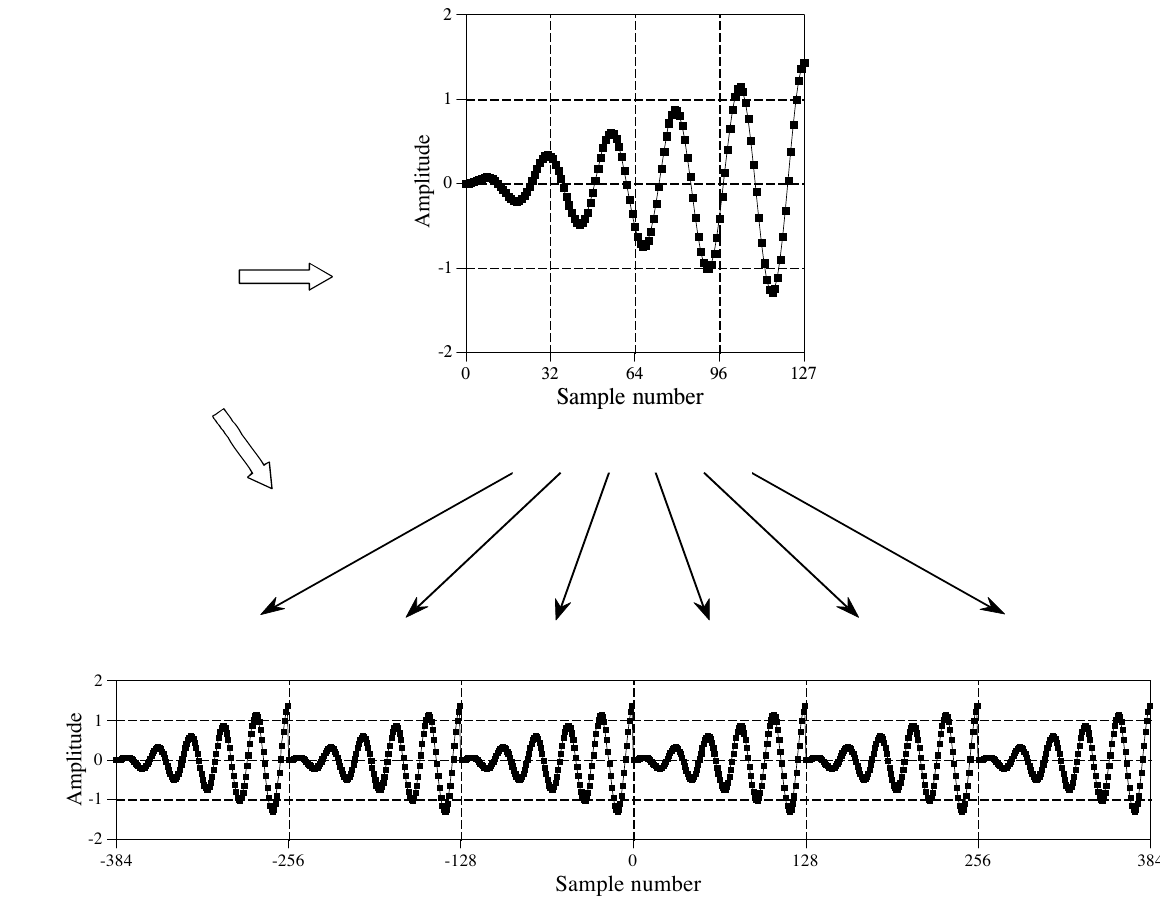
\includegraphics[width=0.967\linewidth,height=0.8\textheight,keepaspectratio]{assets/ch10/fig10-08.png}
\caption*{\textbf{图 10-8　DFT 时域信号的周期性。} 时域既可以看作长度为 N
个采样（上图），也可以看作一个无限长的周期信号（下图）。
（原书在图左侧有两段说明文字，裁图时已去掉：指向上图的箭头旁是 The time
domain viewed as N points = 把时域看作 N 个点；指向下图的箭头旁是 The
time domain viewed as periodic = 把时域看作周期的。Amplitude =
幅度，Sample number = 采样序号。）}
\end{figure}

时域周期性最严重的后果是时域混叠(time domain
aliasing)。为说明这一点，假设我们把一个时域信号送进 DFT
求出它的频谱。我们可以立刻把这个频谱送进逆 DFT
重建出原来的时域信号，但这整个过程没什么意思。我们改为在使用逆 DFT
之前，以某种方式修改频谱。例如，删掉某些频率，改变它们的幅度或相位，把它们挪来挪去，等等。这些都是
DSP
中的家常便饭。遗憾的是，频域中的这些改动可能产生一个太长、一个周期装不下的时域信号。这迫使信号从一个周期溢出到相邻的周期中。把时域看作环形时，信号从右边溢出的部分会突然出现在信号的左边，反之亦然。也就是说，信号溢出的部分把自己混叠到了时域中的一个新位置。如果这个新位置上恰好已经有信号，两者就会搅在一起相加，造成信息丢失。由频域相乘导致的环形卷积(circular
convolution，第 9 章讨论过)，就是这类混叠的绝佳例子。

频域中的周期性表现大体相同，但更复杂一些。图 10-9
是一个例子。上面两幅图是频谱的幅度和相位，看作由分布在采样率 0 到 0.5
之间的 N/2 + 1 个采样组成。这是看待频谱最简单的方式，但它解释不了 DFT
的许多性质。

下面两幅图展示了 DFT 怎样把这个频谱看作周期的。关键特征是：0 到 0.5
之间的频谱，似乎在 0 到 −0.5
之间有一个镜像。这个负频率的镜像，对幅度和相位来说略有不同。对幅度，信号左右翻转；对相位，信号左右翻转并且变号。你应该还记得，这两种对称各有名称：幅度称为偶信号(even
signal，具有偶对称性)，相位称为奇信号(odd
signal，具有奇对称性)。如果把频谱转成实部和虚部，实部总是偶的，虚部总是奇的。

\begin{figure}[htbp]
\centering
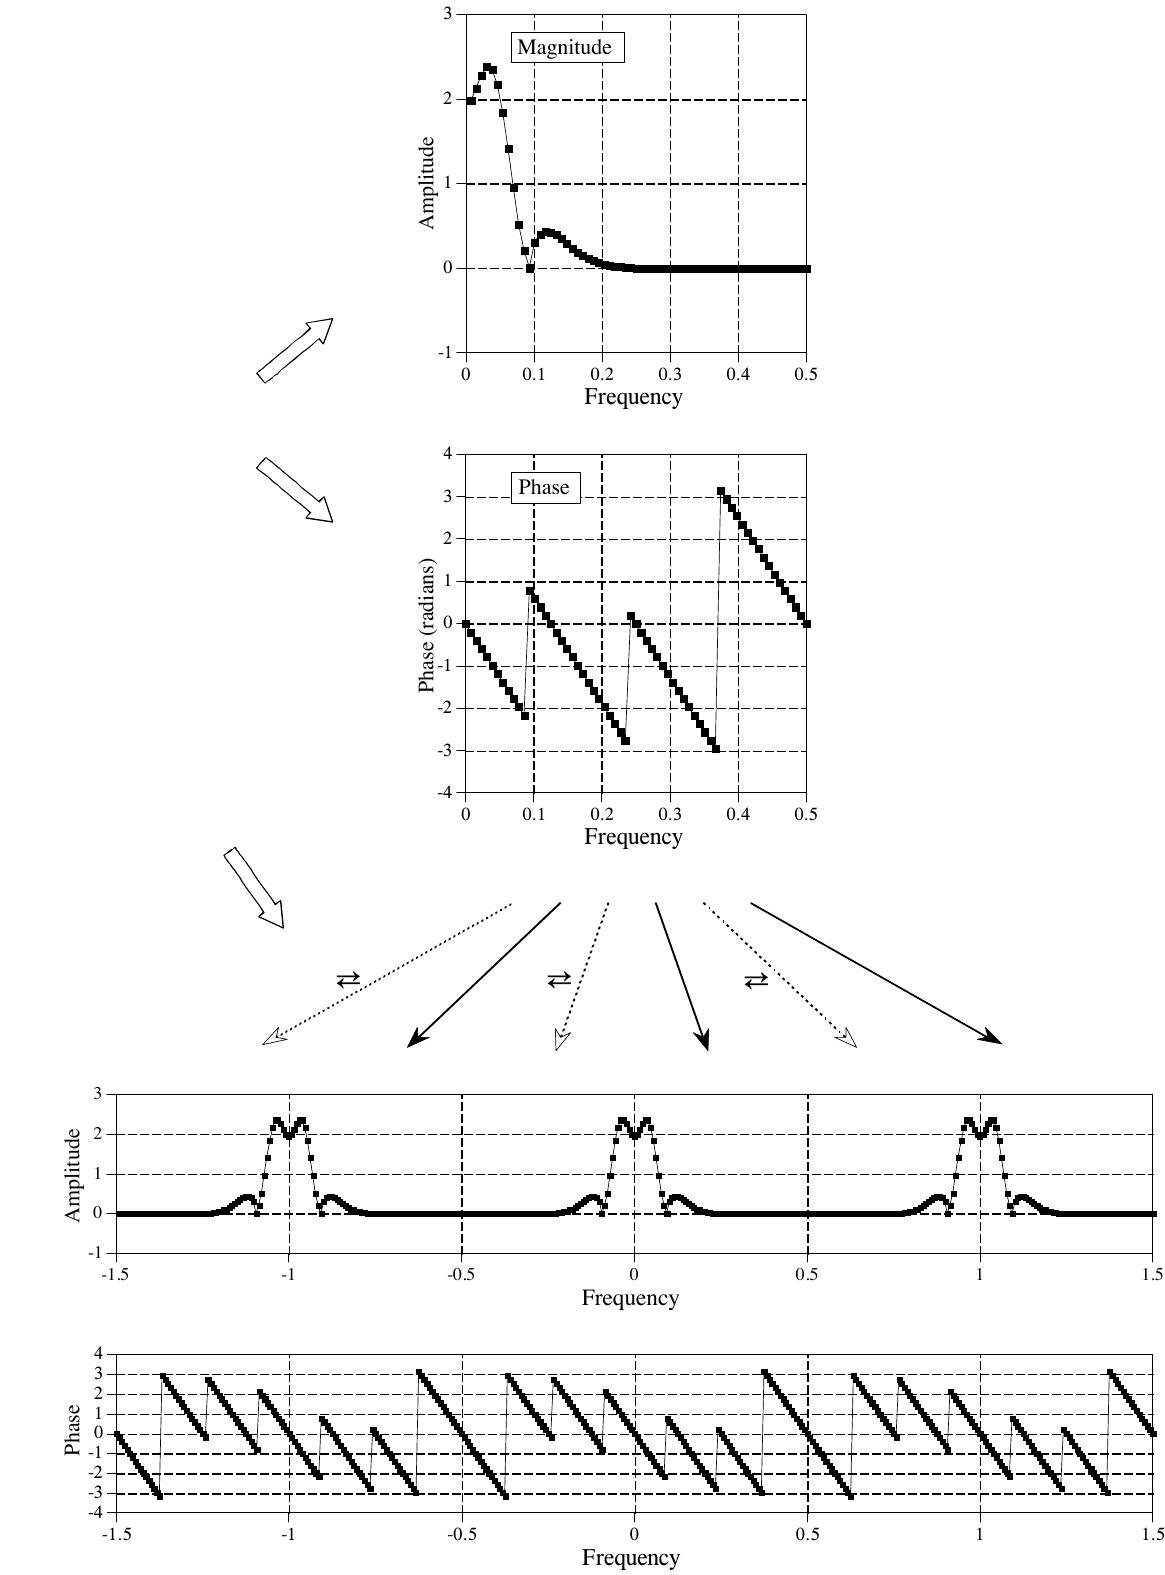
\includegraphics[width=0.971\linewidth,height=0.8\textheight,keepaspectratio]{assets/ch10/fig10-09.png}
\caption*{\textbf{图 10-9　DFT 频域的周期性。} 频域既可以看作从采样率的 0 延伸到
0.5（上面两幅图），也可以看作一个无限长的周期信号，其中每隔一段 0～0.5
的区间就左右翻转一次（下面两幅图）。
（原书在图左侧有两段说明文字，裁图时已去掉：指向上面两幅图的箭头旁是 The
frequency domain viewed as 0 to 0.5 of the sampling rate =
把频域看作采样率的 0 到 0.5；指向下面两幅图的箭头旁是 The frequency
domain viewed as periodic = 把频域看作周期的。Magnitude = 幅度，Phase =
相位，Amplitude = 幅度，Phase (radians) = 相位（弧度），Frequency =
频率；\dspsym{⇄} 表示该段左右翻转。原书图注把 infinitely 误印成
infinity。）}
\end{figure}

把这些负频率考虑在内，DFT 把频域看作周期的，周期为采样率的 1.0 倍，比如
−0.5 到 0.5，或者 0 到 1.0。用采样序号表示，频域一个周期的长度等于
N，与时域相同。

频域的周期性使它容易发生频域混叠(frequency domain
aliasing)，这与前面讲的时域混叠完全类似。设想一个时域信号对应某个频谱。如果修改了这个时域信号，频谱显然也会改变。如果修改后的频谱在给定的空间里放不下，它就会挤进相邻的周期。和前面一样，这种混叠造成两个问题：频率不在它们该在的位置上；来自不同周期的重叠频率相加，破坏了信息。

频域混叠比时域混叠更难理解，因为频域中的周期图案更复杂。考虑一个单一频率，被迫在频域中从
0.01 移动到 0.49。相应的负频率因此从 −0.01 移动到 −0.49。当正频率越过
0.5 这道界线时，负频率也被推过 −0.5
这道界线。由于频域是周期的，同样的事件也在其他周期中发生，比如 0.5 到
1.5 之间。正频率的一个复制品从左向右越过频率
1.5，而负频率的一个复制品从右向左越过 0.5。现在想象一下，如果你只能看到
0 到 0.5
这个频带，会是什么样子：一个从右边离开的频率，又从右边重新出现，但运动方向相反。

图 10-10 说明了只看一个周期时，混叠在时域和频域中是怎样表现的。如 (a)
所示，如果时域信号的一端太长、一个周期装不下，伸出去的那一端会被剪下来贴到另一边。相比之下，(b)
表明频域信号溢出周期时，伸出去的那一端会被折回来。不论混叠的那一段最后落在哪里，它都会与那里原有的信号相加，破坏信息。

\begin{figure}[htbp]
\centering
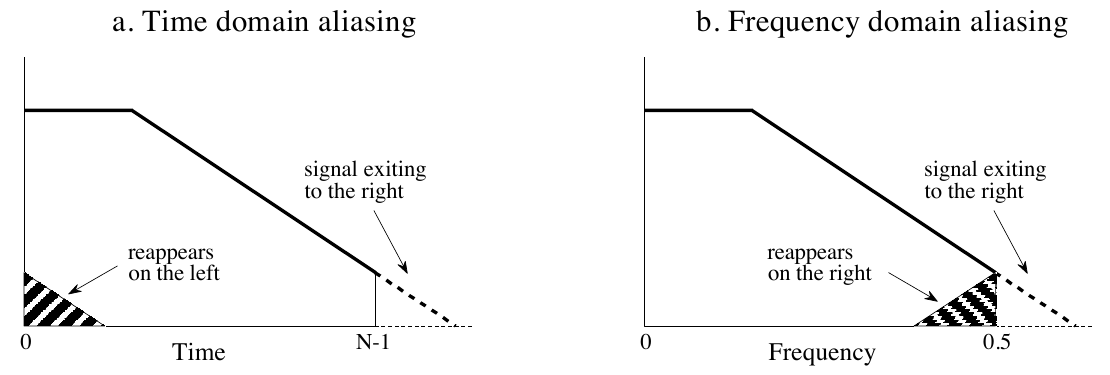
\includegraphics[width=0.925\linewidth,height=0.8\textheight,keepaspectratio]{assets/ch10/fig10-10.png}
\caption*{\textbf{图 10-10　只考虑一个周期时，时域和频域中混叠的例子。}
在时域中，如 (a)
所示，信号从右边出去的部分会从左边重新出现。在频域中，如 (b)
所示，信号从右边出去的部分会从右边重新出现，就像被折回来了一样。 （a.
Time domain aliasing = 时域混叠；b. Frequency domain aliasing =
频域混叠。signal exiting to the right = 从右边出去的信号，reappears on
the left = 从左边重新出现，reappears on the right = 从右边重新出现。Time
= 时间，Frequency = 频率。）}
\end{figure}

我们来仔细看看这些叫做负频率(negative
frequency)的怪东西。它们只是数学的某种古怪产物，还是有真实世界的意义？图
10-11 说明了它们是怎么回事。(a) 是一个由 32
个采样组成的离散信号。设想你的任务是找出这 32
个点对应的频谱。为了让你轻松点，告诉你这些点代表一个离散余弦波。换句话说，你必须找到频率和相移（f
和 θ），使得 \(x[n] = \cos(2\pi n f/N + \theta)\)
与给定的采样相符。你很快就会得到 (b) 所示的解，即 f = 3、θ = −π/4。

如果你的分析到此为止，这道题你只能得 1/3
的分。这是因为还有两个解被你漏掉了。如 (c) 所示，第二个解是 f = −3、θ =
π/4。即使负频率这个想法冒犯了你的感受，也改变不了它是这道题在数学上合法的解这一事实。每个正频率的正弦波，都可以等价地表示成一个负频率的正弦波。这对连续信号和离散信号都适用。

\begin{figure}[htbp]
\centering
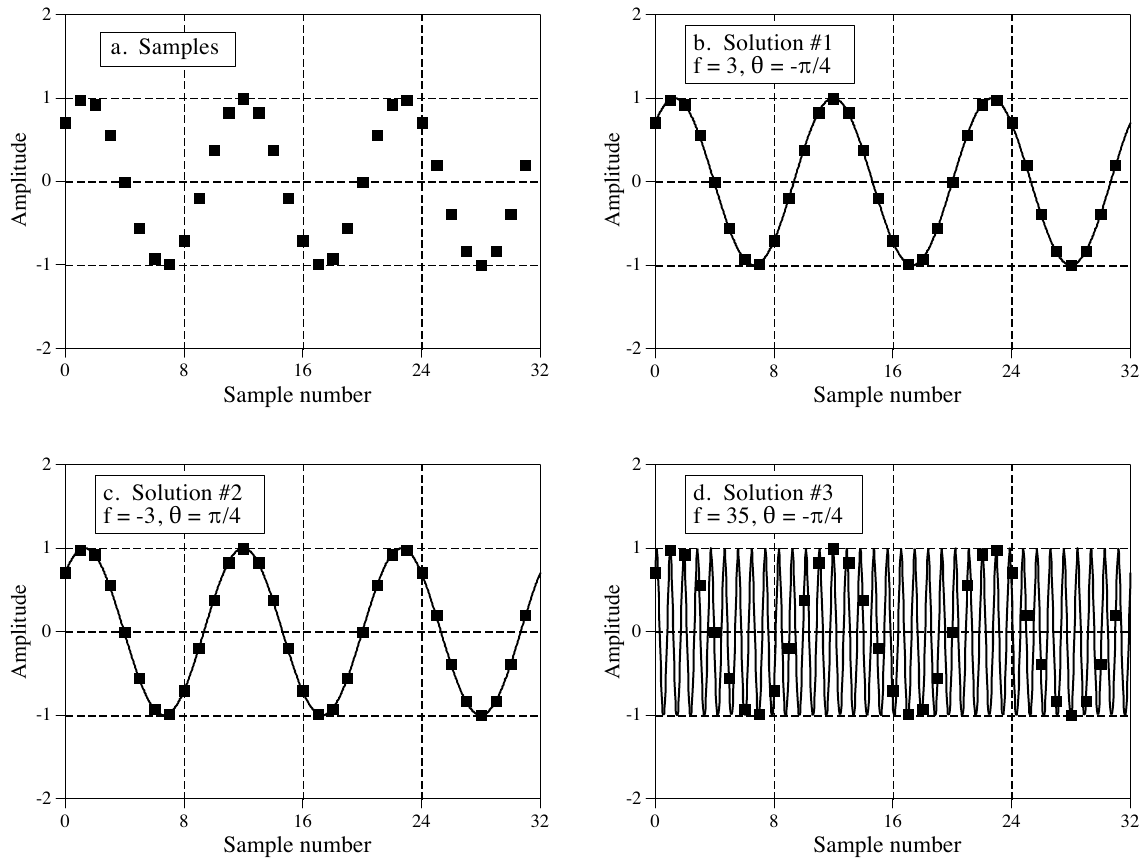
\includegraphics[width=0.950\linewidth,height=0.8\textheight,keepaspectratio]{assets/ch10/fig10-11.png}
\caption*{\textbf{图 10-11　负频率的含义。} 问题是求 (a)
中离散信号的频谱，也就是找出穿过所有采样的那个正弦波的频率和相位。(b)
是用正频率得到的解，(c) 是用负频率得到的解。(d) 代表这个问题的一族解。
（a. Samples = 采样点；b. Solution \#1 = 解 1；c.~Solution \#2 = 解
2；d.~Solution \#3 = 解 3。Amplitude = 幅度，Sample number =
采样序号。）}
\end{figure}

第三个解不是单个答案，而是无穷多个解组成的一族。如 (d) 所示，f = 35、θ =
−π/4
的正弦波穿过所有离散点，因此是一个正确的解。它在采样之间来回振荡，这可能让人困惑，但并不妨碍它成为真正的答案。同样，f
= ±29、f = ±35、f = ±61、f = ±67 都是在点与点之间振荡多次的解。

这三个解各自对应频谱的不同部分。对离散信号来说，第一个解对应采样率 0 到
0.5 之间的频率；第二个解给出 0 到 −0.5 之间的频率；最后，第三个解构成了
−0.5 以下和 0.5
以上无穷多个重复的频率。如果被分析的信号是连续的，第一个解给出从零到正无穷的频率，第二个解给出从零到负无穷的频率，第三组解对连续信号不存在。

许多 DSP 技术不需要使用负频率，也不需要理解 DFT
的周期性。例如，上一章讲的两种常见技术：频谱分析(spectral
analysis)和系统的频率响应(frequency
response)。对这些应用，把时域看作从第 0 个采样到第 N−1
个采样、把频域看作从零到采样频率的一半，就完全够用了。这些技术之所以能用这种更简单的世界观，是因为它们从不会让一个周期的内容跑进另一个周期。在这些情况下，只看一个周期和看整个周期信号效果一样好。

然而，某些处理过程只有考虑信号怎样在周期之间溢出才能分析清楚。前面已经介绍过两个例子：环形卷积和模数转换(analog-to-digital
conversion)。在环形卷积中，频谱相乘导致时域信号做卷积。如果得到的时域信号太长、一个周期装不下，它就会溢出到相邻周期中，造成时域混叠。相反，模数转换是频域混叠的一个例子。在时域中进行了一个非线性操作，即通过采样把连续信号变成离散信号。问题在于，原始模拟信号的频谱可能太长，离散信号的频谱装不下。硬要这样做，频谱的两端就会伸进相邻的周期。我们再看两个
DFT 周期性很重要的例子：信号的压缩与扩展，以及幅度调制。

\section{压缩与扩展，多速率方法}

如图 10-12
所示，信号在一个域里压缩，就会在另一个域里扩展，反之亦然。对连续信号，如果
X(f) 是 x(t) 的傅里叶变换，那么 \(\frac{1}{k} X(f/k)\) 就是 \(x(kt)\)
的傅里叶变换，其中 k
是控制扩展或压缩的参数。如果一个事件发生得更快（在时间上被压缩），它必然由更高的频率组成；如果一个事件发生得更慢（在时间上被扩展），它必然由更低的频率组成。把这个规律推向两个极端也成立。也就是说，如果时域信号被压缩得变成了一个冲激，相应的频谱就被扩展得变成一个常数。同样，如果时域被扩展得变成一个常数，频域就变成一个冲激。

\begin{quote}
\textbf{译注：} 原书写的是 1/k × X(f/k)。严格地说，当 k 为负数时系数应为
1/\textbar k\textbar；这里 k 只表示压缩或扩展的倍数，取正数即可。
\end{quote}

\begin{figure}[htbp]
\centering
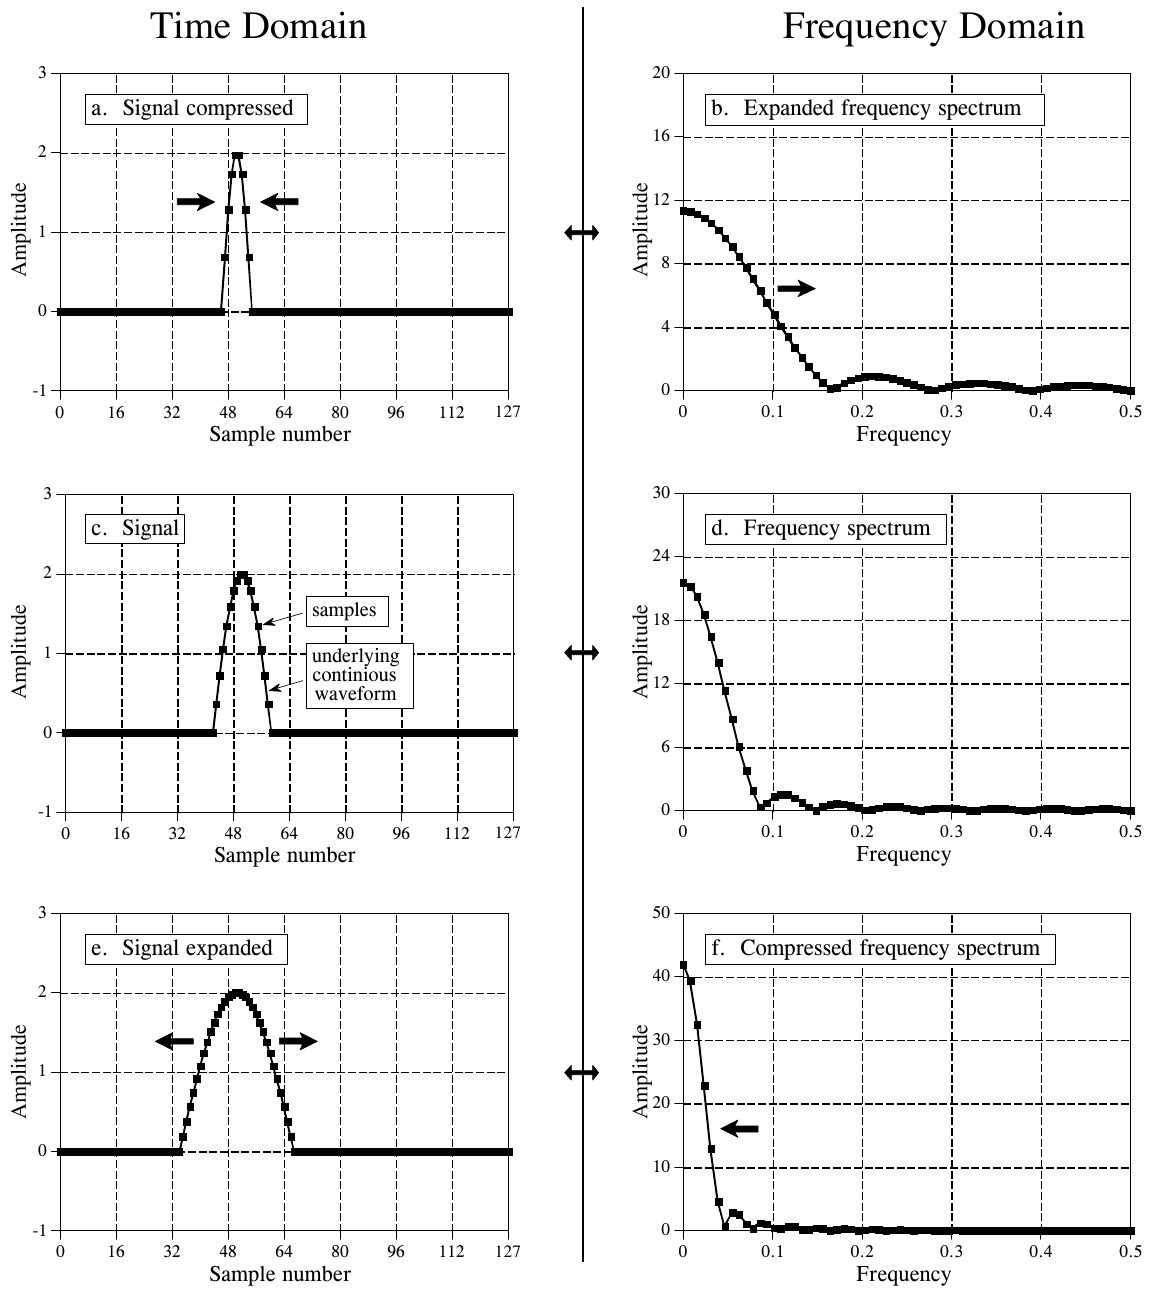
\includegraphics[width=0.958\linewidth,height=0.8\textheight,keepaspectratio]{assets/ch10/fig10-12.png}
\caption*{\textbf{图 10-12　压缩与扩展。}
在一个域里压缩信号，会使信号在另一个域里扩展，反之亦然。(c) 和 (d)
分别是一个离散信号及其频谱。在 (a) 和 (b)
中，时域信号被压缩，导致频谱被扩展。(e) 和 (f)
展示的是相反的过程。如图所示，离散信号的扩展或压缩，是通过扩展或压缩其背后的连续波形来实现的，然后对这条背后的波形重新采样，得到新的离散信号。
（Time Domain = 时域，Frequency Domain = 频域；a. Signal compressed =
压缩后的信号，b. Expanded frequency spectrum = 扩展后的频谱，c.~Signal =
信号，d.~Frequency spectrum = 频谱，e. Signal expanded =
扩展后的信号，f.~Compressed frequency spectrum = 压缩后的频谱；samples =
采样点，underlying continuous waveform = 背后的连续波形（图中误拼为
continious）。Amplitude = 幅度，Sample number = 采样序号，Frequency =
频率。）}
\end{figure}

离散信号的表现与此类似，但有更多细节。离散信号的第一个问题是混叠。设想
(a) 中的脉冲比图中所示再压缩好几倍。频谱会扩展同样的倍数，(b)
中的几个驼峰会被推到 0.5
以上的频率。由此产生的混叠，打破了简单的扩展/压缩关系。这类混叠也可能发生在时域中。设想
(f) 中的频谱被压缩得更狠，导致 (e) 中的时域信号扩展到相邻的周期里。

第二个问题是要准确定义压缩或扩展一个离散信号是什么意思。如图 10-12a
所示，压缩离散信号的方法是：把采样点所在的那条背后的连续曲线压缩，再对新的连续曲线重新采样，得到新的离散信号。同样，(e)
展示了用同样的过程扩展离散信号。离散信号被压缩时，信号中的事件（比如脉冲的宽度）在更少的采样内发生；同样，扩展后的信号中的事件在更多的采样内发生。

看待这一过程的另一种等价方式是：背后的连续波形保持不变，但以不同的采样率重新采样。例如，看图
10-13a，一个由 50 个采样组成的离散高斯波形。在 (b)
中，同一条背后的曲线用 400 个采样来表示。(a) 到 (b)
的变化可以从两方面看：(1)
采样率保持不变，但背后的波形被扩展到八倍宽；或者 (2)
背后的波形保持不变，但采样率提高到八倍。以这种方式改变采样率的方法叫多速率技术(multirate
techniques)。如果增加了采样，叫插值(interpolation)；如果用更少的采样表示信号，叫抽取(decimation)。第
3 章讲过多速率技术在 ADC 和 DAC 中的应用。

问题来了：给定一个任意的离散信号，我们怎么知道它背后的连续曲线是什么？这取决于信号的信息是编码在时域中还是频域中。对于时域编码的信号，我们希望背后的连续波形是一条穿过所有采样的平滑曲线。最简单的做法，可以在点与点之间画直线，再把粗糙的拐角磨圆。更进一步，可以用曲线拟合算法，比如样条函数(spline
function)或多项式拟合。这个问题没有唯一''正确''的答案。这种方法的出发点是让时域波形中的不规则性最小，完全不考虑频域。

当信号的信息编码在频域中时，我们不管时域波形，而专注于频谱。上一章讲过，在做
DFT 之前给时域信号补零，就能得到更精细的频谱采样（频率 0 到 0.5
之间的采样更多）。对偶性(duality)让这一做法可以反过来用：如果想在时域中得到更精细的采样（插值），就在做逆
DFT 之前给频谱补零。假设我们想把一个 50 点的信号插值成 400
点的信号，做法如下：(1) 取这 50 个采样，补零使信号长 64 个采样。(2) 用
64 点 DFT 求出频谱，它由 33 点的实部和 33 点的虚部组成。(3)
在频谱的右边（实部和虚部都要）补 224 个零，使频谱长 257 点。(4) 用 512
点逆 DFT 把数据变回时域。这样得到一个 512 点的信号，它是那个 64
点信号的高分辨率版本。这个信号的前 400 个采样，就是原来 50
个采样的插值版本。

\begin{figure}[htbp]
\centering
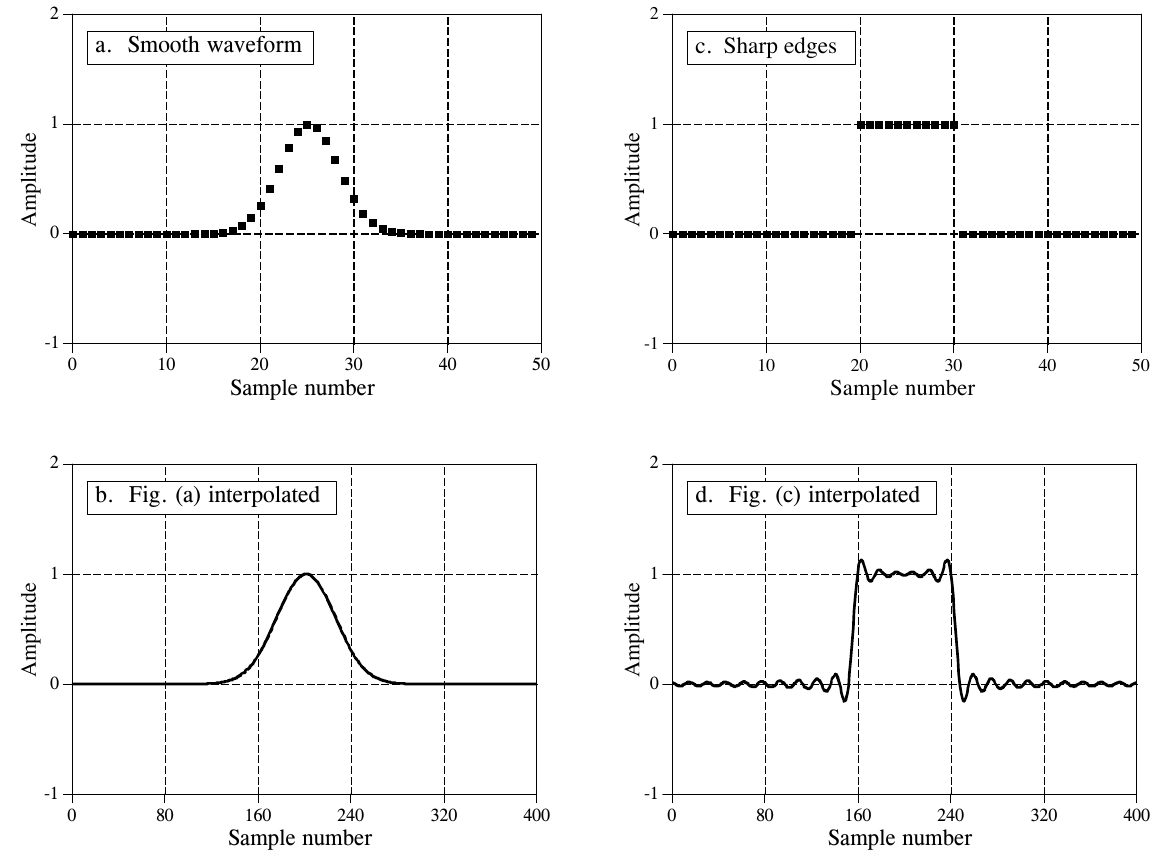
\includegraphics[width=0.963\linewidth,height=0.8\textheight,keepaspectratio]{assets/ch10/fig10-13.png}
\caption*{\textbf{图 10-13　通过在频域补零来插值。} (a) 和 (c) 各由 50
个采样组成。通过在频域补零，把它们插值成 400 个采样，分别得到 (b) 和
(d)。（(b) 和 (d) 是离散信号，但因为采样数很多，画成了连续的线。） （a.
Smooth waveform = 平滑波形；b. Fig. (a) interpolated = 图 (a)
插值后；c.~Sharp edges = 陡峭的边沿；d.~Fig. (c) interpolated = 图 (c)
插值后。Amplitude = 幅度，Sample number = 采样序号。）}
\end{figure}

这种技术的关键特点是：插值后的信号与原信号由完全相同的频率组成。这在时域中不一定能给出一个表现良好的拟合。例如，图
10-13 (a) 和 (b) 展示了用这种方法把一个 50 点信号插值成 400
点信号。插值结果是原始点之间的一条平滑拟合，就像用了曲线拟合程序一样。相比之下，(c)
和 (d) 展示了另一个例子，时域一团糟！(d)
中的振荡出现在信号的边沿或其他不连续处。由于时域被看作环形的，这也包括第
0 个采样与第 N−1
个采样之间的任何不连续。这种在不连续处的过冲叫吉布斯效应(Gibbs
effect)，第 11 章会讨论。第 3
章还介绍了另一种频域插值技术：在时域采样之间插入零，再做低通滤波。

\section{信号相乘（幅度调制）}

傅里叶变换的一个重要性质是：一个域里的卷积对应另一个域里的相乘。上一章讨论了其中一面：时域信号可以通过把它们的频谱相乘来卷积。幅度调制(amplitude
modulation)是相反情形的一个例子：时域里的相乘对应频域里的卷积。此外，幅度调制还是一个极好的例子，说明难以捉摸的负频率是怎样进入日常科学和工程问题的。

音频信号很适合短距离通信：你说话时，屋子那头的人能听见。另一方面，无线电频率非常擅长远距离传播。例如，把一个
100 伏、1 MHz
的正弦波送进天线，产生的无线电波在隔壁房间、隔壁国家，甚至隔壁星球都能被探测到。调制(modulation)就是把两个信号融合成第三个信号、让它兼具两者理想特性的过程。这总要用到非线性过程，比如相乘；不能只是把两个信号加起来。在无线电通信中，调制得到的无线电信号既能远距离传播，又能携带音频或其他信息。

无线电通信是一门极其成熟的学科，人们开发了许多调制方案。最简单的一种叫幅度调制。图
10-14
是幅度调制在时域和频域中表现的一个例子。本例使用连续信号，因为调制通常在模拟电子电路中完成。不过如果需要，整个过程也可以用离散形式完成（这是未来的方向！）。

\begin{enumerate}
\def\labelenumi{(\alph{enumi})}
\tightlist
\item
  是一个加了直流偏置、使信号始终为正值的音频信号。(b) 显示它的频谱由 300
  Hz 到 3 kHz
  的频率（语音通信所需的频率范围）以及代表直流分量的一根尖峰组成。其他所有频率都已被模拟滤波去掉。(c)
  和 (d) 是载波(carrier
  wave)，一个频率比音频信号高得多的纯正弦波。在时域中，幅度调制就是把音频信号乘以载波。如
  (e)
  所示，结果是一个振荡波形，它的瞬时幅度与原音频信号成正比。用这一行的行话说，载波的包络(envelope)等于调制信号。这个信号可以送到天线，变成无线电波，再被接收天线探测到。这样，在无线电接收机的电子电路中就会产生一个与
  (e) 相同的信号。然后用检波器(detector)或解调器(demodulator)电路，把
  (e) 中的波形变回 (a) 中的波形。
\end{enumerate}

由于时域信号相乘，对应的频谱就做卷积。也就是说，(f) 是 (b) 与 (d)
卷积得到的。由于载波的频谱是一个平移过的冲激函数，调制信号的频谱就等于把音频频谱平移到载波频率处。这样得到的调制频谱由三个分量组成：载波、上边带(upper
sideband)和下边带(lower sideband)。

\begin{figure}[htbp]
\centering
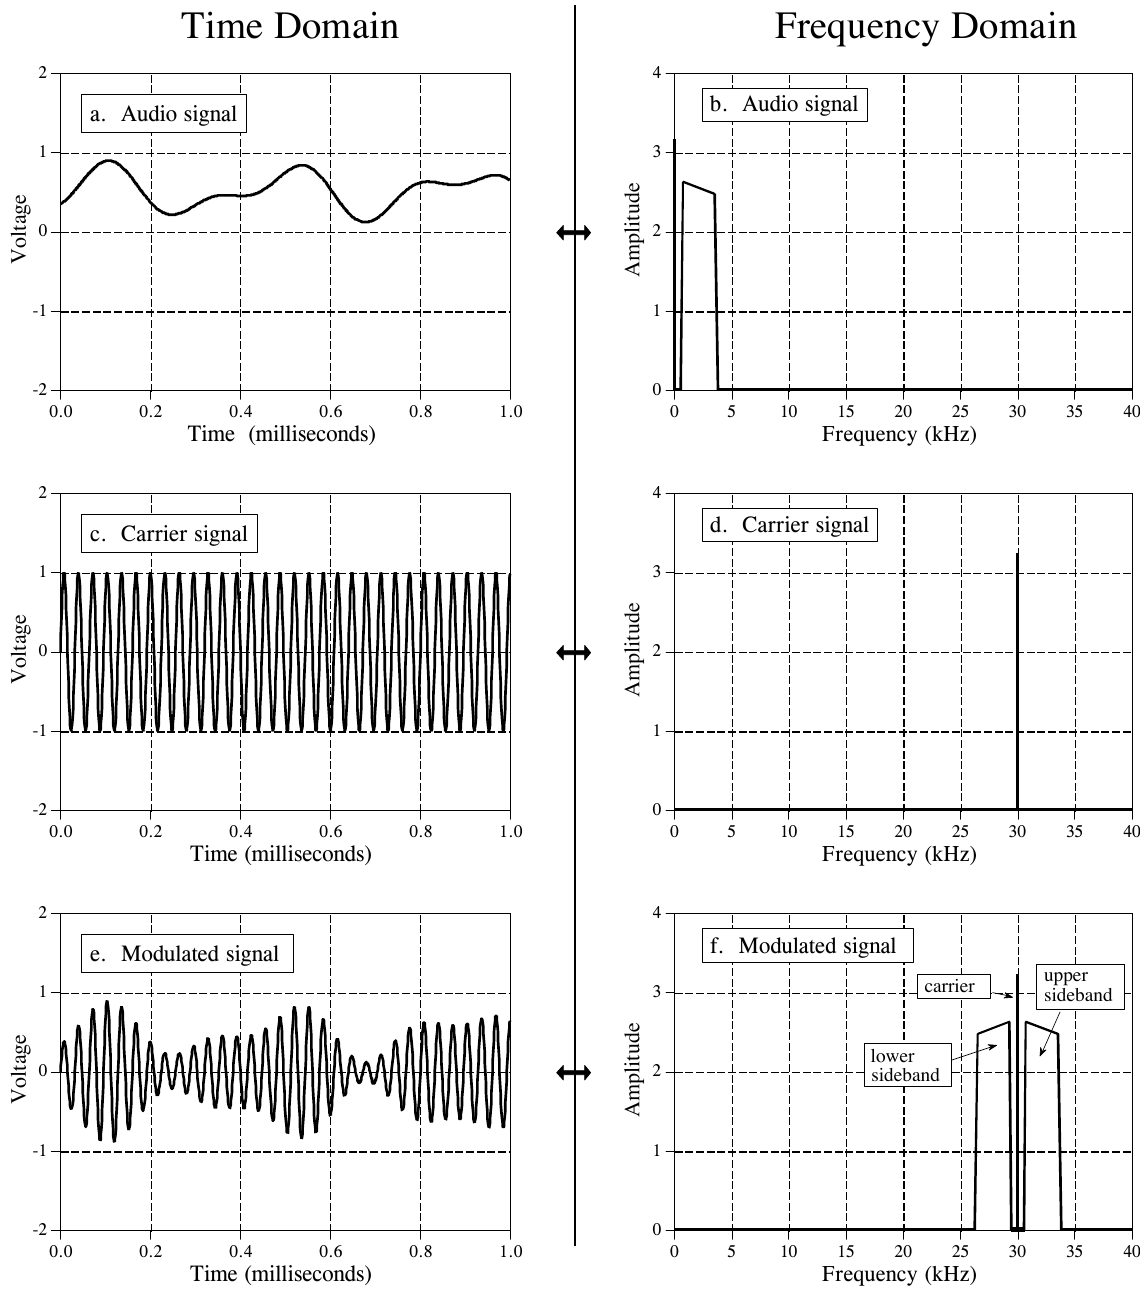
\includegraphics[width=0.950\linewidth,height=0.8\textheight,keepaspectratio]{assets/ch10/fig10-14.png}
\caption*{\textbf{图 10-14　幅度调制。} 在时域中，幅度调制是把音频信号 (a)
乘以载波信号 (c)，得到调制信号
(e)。由于时域相乘对应频域卷积，调制信号的频谱就是把音频信号的频谱平移到载波频率处。
（Time Domain = 时域，Frequency Domain = 频域；a、b. Audio signal =
音频信号，c、d.~Carrier signal = 载波信号，e、f.~Modulated signal =
调制信号；carrier = 载波，upper sideband = 上边带，lower sideband =
下边带。Voltage = 电压，Amplitude = 幅度，Time (milliseconds) =
时间（毫秒），Frequency (kHz) = 频率（kHz）。）}
\end{figure}

这三个分量依次对应原音频信号的三个部分：直流分量、0.3 到 3 kHz
之间的正频率，以及 −0.3 到 −3 kHz
之间的负频率。尽管原音频信号中的负频率有些难以捉摸、比较抽象，下边带里的频率却真实得不能再真实了。幽灵化成人形了！

通信工程师的饭碗就靠这类频域分析。例如，考虑电视传输的频谱。一路标准电视信号的频谱从直流到
6 MHz。利用这些频率平移技术，82 个这样 6 MHz
宽的频道首尾相接地排列起来。例如，第 3 频道是 60 到 66 MHz，第 4 频道是
66 到 72 MHz，第 83 频道是 884 到 890
MHz，等等。电视接收机把想看的频道挪回直流到 6 MHz
的频带，再显示到屏幕上。这种方案叫频分复用(frequency domain
multiplexing)。

\section{离散时间傅里叶变换}

离散时间傅里叶变换（Discrete Time Fourier
Transform，DTFT）是傅里叶变换家族中处理非周期离散信号的成员。理解 DTFT
最好的方式，是看它和 DFT 的关系。首先，设想你采集了一个 N
点信号，想求它的频谱。用 DFT 可以把信号分解成 N/2 + 1
个正弦波和余弦波，它们的频率在零到采样率一半之间等间隔分布。上一章讲过，给时域信号补零，会让时域的周期变长，同时让频域采样之间的间隔变窄。当
N 趋于无穷大时，时域变成非周期的，频域变成连续信号。这就是
DTFT：把一个非周期的离散信号，与一个周期的连续频谱联系起来的傅里叶变换。

理解 DTFT 的数学，可以从 DFT 的合成和分析公式（公式 8-2、8-3 和
8-4）出发，让 N 趋于无穷大：

\textbf{公式 10-1}　DTFT 的分析公式。式中 x{[}n{]}
是时域信号，频谱存放在 Re X(ω) 和 Im X(ω) 中，ω 的取值范围是 0 到 π。

\[\mathrm{Re}\,X(\omega) = \sum_{n=-\infty}^{+\infty} x[n]\cos(\omega n)\]

\[\mathrm{Im}\,X(\omega) = -\sum_{n=-\infty}^{+\infty} x[n]\sin(\omega n)\]

\textbf{公式 10-2}　DTFT 的合成公式。

\[x[n] = \frac{1}{\pi}\int_{0}^{\pi} \big[\mathrm{Re}\,X(\omega)\cos(\omega n) - \mathrm{Im}\,X(\omega)\sin(\omega n)\big]\,d\omega\]

\begin{quote}
\textbf{译注：} 原书公式 10-1 的说明写''n 从 0 到
N−1''，与公式本身的求和范围（−\dspsym{∞} 到 +\dspsym{∞}）不一致；DTFT
处理的是无限长的非周期信号，应以公式为准。说明的最后一句在原书版面上只印到''ω
的取值''就断了，按正文补为 0 到 π。
\end{quote}

这些关系中有许多微妙的细节。首先，时域信号 x{[}n{]}
仍然是离散的，因此用方括号表示。相比之下，频域信号 Re X(ω) 和 Im X(ω)
是连续的，因此用圆括号表示。由于频域是连续的，合成公式必须写成积分，而不是求和。

第 8 章讲过，在 DFT 的频域中，频率用三个变量之一来表示：k，一个从 0 到
N/2 的索引；f，采样率的分数，从 0 到 0.5；或者
ω，用自然频率表示的采样率分数，从 0 到 π。DTFT 的频谱是连续的，所以 f 或
ω 都可以用。常见的选择是 ω，因为它省掉了总是出现的 2π
因子，让公式更短。记住，用 ω 时，频谱从 0 延伸到
π，对应直流到采样率的一半。更复杂的是，许多作者在 DTFT 中用 Ω（大写的
omega）而不是 ω（小写的 omega）来表示这个频率。

计算逆 DFT 时，必须先把第 0 个和第 N/2 个采样除以二（公式
8-3），才能进行合成（公式 8-2）。DTFT 不需要这一步。你应该还记得，DFT
中的这一操作与把频谱定义为谱密度(spectral
density)有关，即单位带宽上的幅度。当频谱变成连续的，对端点的特殊处理就消失了。不过，仍然有一个必须包含的归一化因子：DFT
中的 2/N（公式 8-3）在 DTFT 中变成了 1/π（公式
10-2）。有的作者把这些项放在合成公式前面，有的放在分析公式前面。假设你从某个时域信号出发，做傅里叶变换，再做逆傅里叶变换，你希望最后得到的就是开始的那个信号。也就是说，1/π
这一项（或者 2/N
这一项）必须在正变换或逆变换的某个环节出现。有的作者甚至把这一项拆开放到两个变换中，在两者前面都放上
\(1/\sqrt{\pi}\)。

由于 DTFT
涉及无穷求和与积分，它无法用数字计算机算出来。它的主要用途是在理论问题中替代
DFT。例如，假设你想由系统的冲激响应求出它的频率响应。如果冲激响应是一个数组，比如由实验测量或计算机仿真得到的，就在计算机上运行
DFT 程序。这会得到另一个数组形式的频谱，在采样率的 0 到 0.5
之间等间隔分布。

在另一些情况下，冲激响应可能是以公式的形式已知的，比如 sinc
函数（下一章介绍）或指数衰减的正弦波。这时就用
DTFT，以数学方法把频域算成另一个公式，给出 0 到 0.5
之间整条连续曲线。虽然这个计算也可以用 DFT 来做，但 DFT
只能给出频率响应采样点的公式，而不是整条曲线。

\section{帕塞瓦尔关系}

既然时域和频域是同一个信号的两种等价表示，它们就必须具有相同的能量。这叫帕塞瓦尔关系(Parseval's
relation)，对傅里叶变换家族的所有成员都成立。对
DFT，帕塞瓦尔关系表示为：

\textbf{公式 10-3}　帕塞瓦尔关系。式中 x{[}i{]} 是时域信号，i 从 0 到
N−1；X{[}k{]} 是它修正后的频谱，k 从 0 到
N/2。修正后的频谱这样得到：对信号做 DFT，再把第一个和最后一个频率（第 0
个和第 N/2 个采样）除以 2 的平方根。

\[\sum_{i=0}^{N-1} x[i]^2 = \frac{2}{N}\sum_{k=0}^{N/2} \mathrm{Mag}\,X[k]^2\]

等式左边是时域信号包含的总能量，通过把 N
个单独采样的能量加起来得到。同样，右边是频域包含的能量，通过把 N/2 + 1
个正弦波的能量加起来得到。物理学告诉我们，能量与幅度的平方成正比。例如，弹簧中的能量与位移的平方成正比，电容器中储存的能量与电压的平方成正比。在公式
10-3 中，X{[}f{]} 是 x{[}n{]}
的频谱，只有一点小修改：第一个和最后一个频率分量 X{[}0{]} 和 X{[}N/2{]}
被除以了 \(\sqrt{2}\)。这一修改，加上等式右边的 2/N
因子，处理了计算和累加能量时的几个微妙细节。

要理解这些修正，先用 DFT
求出信号的频域表示。然后，把频域转换成重建信号所需的正弦波幅度，即公式
8-3 中定义的那样：把第一个和最后一个点（第 0 个和第 N/2 个采样）除以
2，再把所有点除以 N/2。这样得到的是正弦波的幅度，但它们是峰值幅度(peak
amplitude)，而不是计算能量所需的均方根(root-mean-square，rms)幅度。对正弦波，把峰值幅度除以
\(\sqrt{2}\) 就转换成 rms 值。除了第 0 个和第 N/2
个采样，所有频域值都必须做这个修正。这是因为这两个正弦波很特殊：一个是常数，另一个在两个常数值之间交替。对这两个特殊情形，峰值幅度本来就等于
rms 值。频域中所有的值平方后再求和。最后一步是把求和结果除以
N，这是因为频域中的每个采样都被转换成一个覆盖时域 N
个值的正弦波。把这些细节都处理完，就得到公式 10-3。

帕塞瓦尔关系所描述的物理（能量守恒）很有意思，但它在 DSP
中的实际用处不多。

% !TEX root = ../main.tex
% 本文件由 build-tex.sh 从 11-DSP指南-第11章中译.md 生成，改内容请改 md 后重新生成

\chapter{傅里叶变换对}\label{ch-11}

每个时域波形都有一个对应的频域波形，反过来也一样。例如，时域中的矩形脉冲(rectangular
pulse)对应频域中的 sinc 函数（即
sin(x)/x）。对偶性(duality)保证反过来也成立：频域中的矩形脉冲对应时域中的
sinc 函数。像这样彼此对应的波形叫做傅里叶变换对(Fourier transform
pair)。本章介绍几种常见的变换对。

\section{冲激函数变换对}

对离散信号来说，冲激函数(delta
function)是一个简单的波形，它的傅里叶变换对也同样简单。图 11-1a
是时域中的一个冲激函数，(b) 和 (c)
是它的频谱。幅度(magnitude)是一个常数，相位(phase)则处处为零。上一章讲过，这可以用扩展/压缩性质(expansion/compression
property)来理解：时域被压缩到变成一个冲激时，频域就被扩展到变成一个常数。

在 (d) 和 (g) 中，时域波形分别向右平移了 4 个和 8
个采样。正如上一章的性质所预期的，时域波形的平移不影响幅度，但给相位加上了一个线性分量。本图中的相位信号没有展开(unwrapped)，所以只在
−π 到 π 之间。还要注意，频域的横轴从 −0.5 到
0.5，也就是说，图中除了正频率还画出了频谱的负频率(negative
frequencies)。负频率是冗余信息，但 DSP
的图里经常会画上它们，你应该习惯看到它们。

\begin{figure}[htbp]
\centering
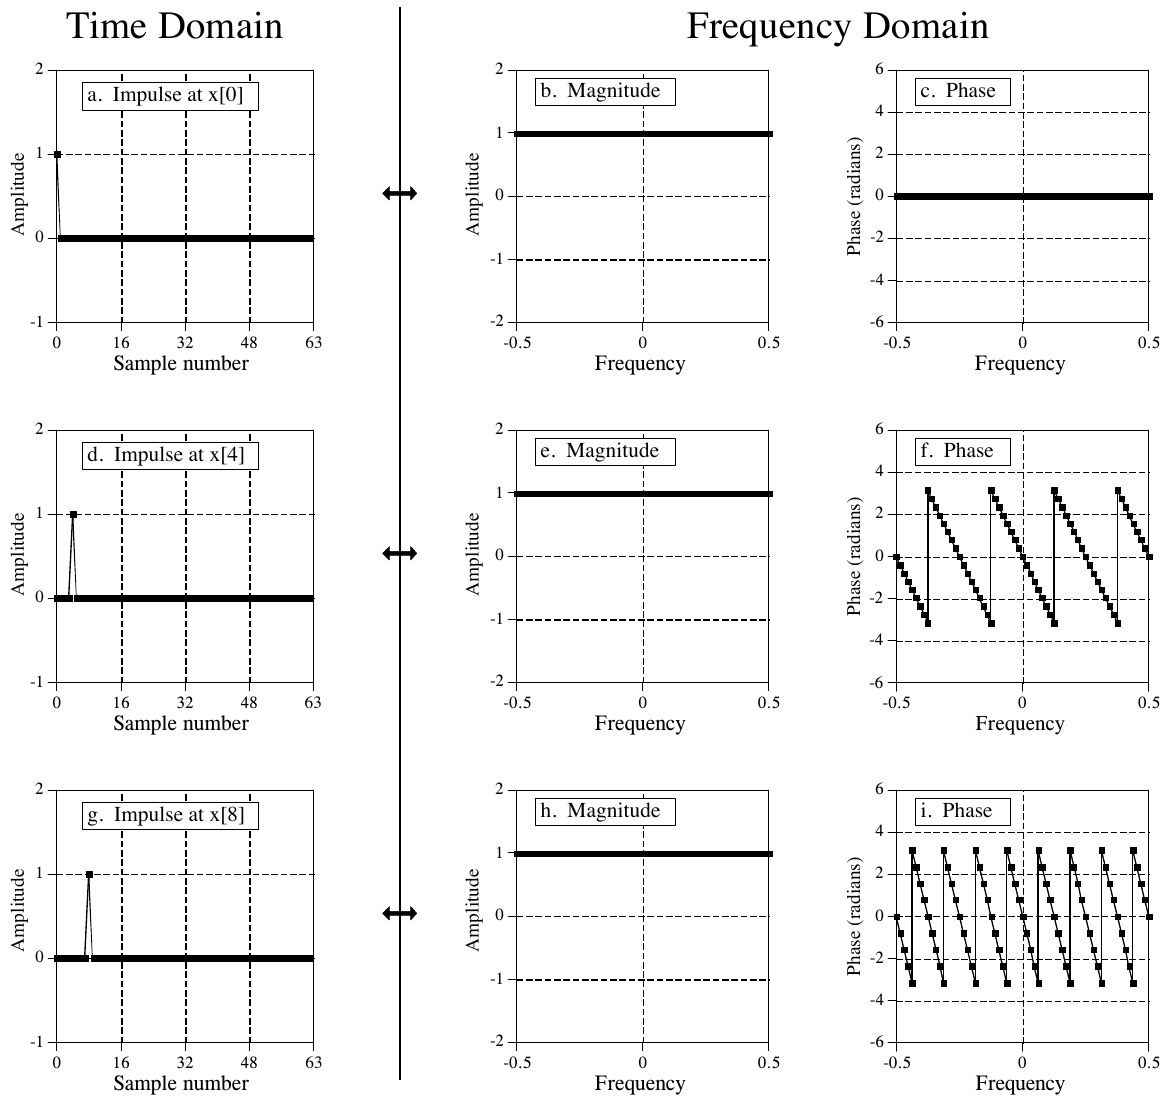
\includegraphics[width=0.975\linewidth,height=0.8\textheight,keepaspectratio]{assets/ch11/fig11-01.png}
\caption*{\textbf{图 11-1　极坐标形式的冲激函数变换对。}
时域中的一个冲激，对应频域中的常数幅度和线性相位。 （Time Domain =
时域，Frequency Domain = 频域；a. Impulse at x{[}0{]} = 位于 x{[}0{]}
的冲激，b. Magnitude = 幅度，c.~Phase = 相位；d、g 分别是位于
x{[}4{]}、x{[}8{]} 的冲激，e、h 为幅度，f、i 为相位。Amplitude =
幅度，Phase (radians) = 相位（弧度），Sample number =
采样序号，Frequency = 频率；中间的 \dspsym{↔} 表示左右两边互为变换对。）}
\end{figure}

图 11-2 给出了与图 11-1 相同的信息，只是频域改用直角坐标形式(rectangular
form)表示。这里有两点值得学习。第一，比较频域的极坐标表示和直角坐标表示。和通常一样，极坐标形式要好理解得多：幅度只是一个常数，相位是一条直线。相比之下，实部和虚部是正弦振荡，很难说出它们代表什么意思。

\begin{figure}[htbp]
\centering
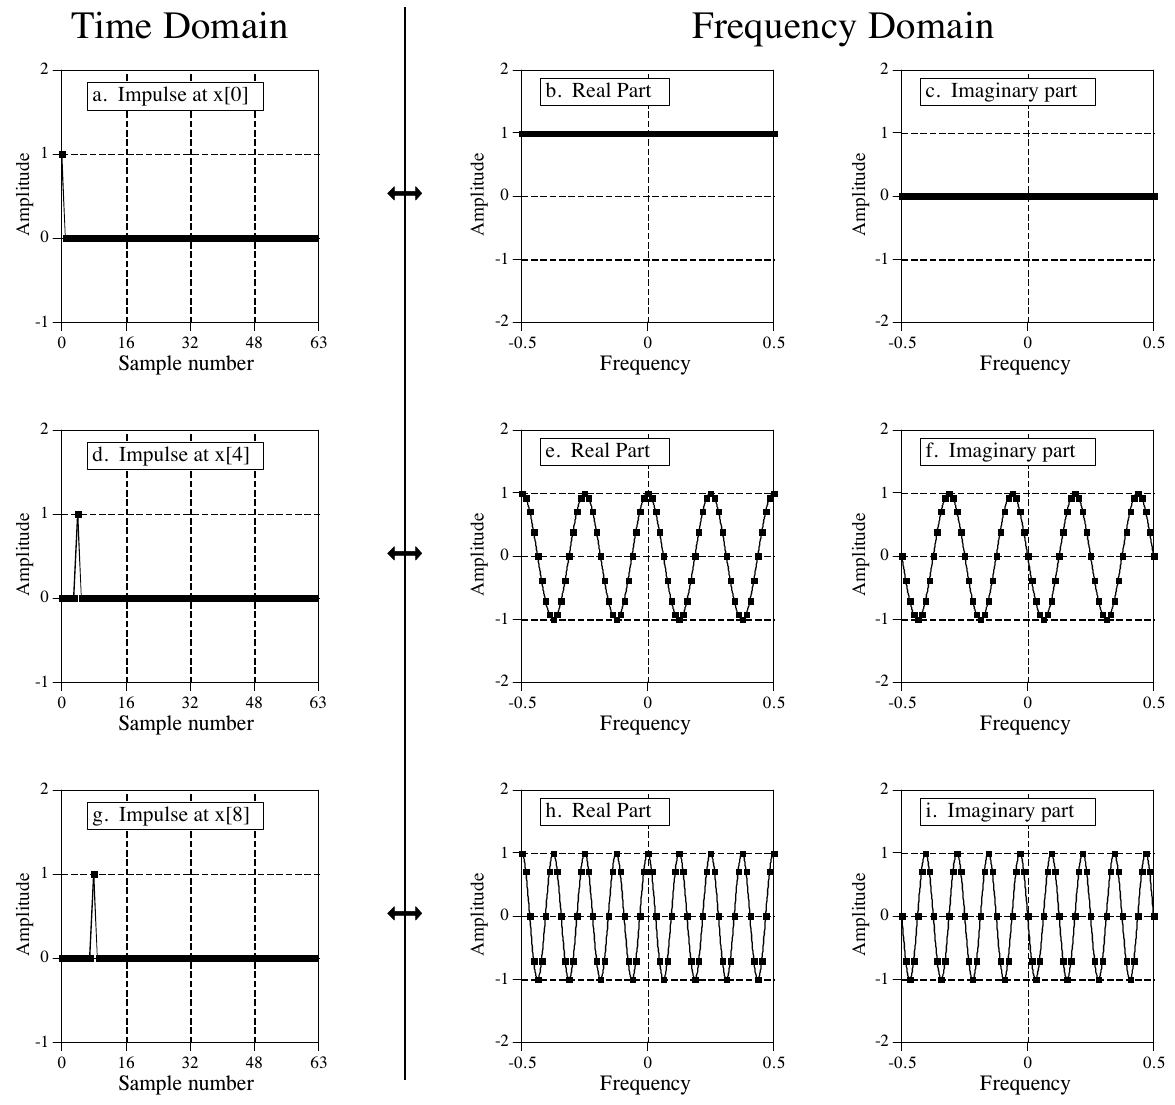
\includegraphics[width=0.979\linewidth,height=0.8\textheight,keepaspectratio]{assets/ch11/fig11-02.png}
\caption*{\textbf{图 11-2　直角坐标形式的冲激函数变换对。}
时域中的每个采样，在频域的实部产生一个余弦波，在虚部产生一个负的正弦波。
（Time Domain = 时域，Frequency Domain = 频域；a、d、g. Impulse at
x{[}0{]}/x{[}4{]}/x{[}8{]} = 位于 x{[}0{]}/x{[}4{]}/x{[}8{]}
的冲激；b、e、h. Real Part = 实部；c、f、i. Imaginary part =
虚部。Amplitude = 幅度，Sample number = 采样序号，Frequency = 频率。）}
\end{figure}

图 11-2 的第二个有趣之处是 DFT 的对偶性。按通常的看法，DFT
频域中的每个采样对应时域中的一个正弦信号(sinusoid)。然而反过来也成立：时域中的每个采样对应频域中的正弦信号。在图中画出负频率，能让对偶性显得更对称。例如，图
(d)、(e)、(f) 表明，时域中第 4 个采样处的一个冲激，在频谱的实部产生 4
个周期的余弦波，在虚部产生 4 个周期的负正弦波。回想一下，频谱实部第 4
个采样处的冲激，在时域产生 4 个周期的余弦波；同样，频谱虚部第 4
个采样处的冲激，会在时域波形上叠加 4 个周期的负正弦波。

第 8 章提到过，这可以用作计算 DFT
的另一种方法（除了把时域信号与正弦信号做相关之外）。时域中的每个采样，都会在频域实部加上一个余弦波，在虚部加上一个负正弦波。每个正弦信号的幅度由该时域采样的幅度给出，频率由该时域点的采样序号给出。算法步骤是：(1)
逐个遍历时域采样；(2) 算出每个采样对应的正弦波和余弦波；(3)
把所有贡献的正弦信号加起来。得到的程序和相关法（表
8-2）几乎一模一样，只是内外两层循环互换了。

\section{sinc 函数}

图 11-3 展示了一个常见的变换对：矩形脉冲与 sinc 函数(sinc function，读作
``sink'')。sinc 函数的定义是
\(\mathrm{sinc}(a) = \sin(\pi a)/(\pi a)\)，不过常见到一种含糊的说法：``sinc
函数的一般形式是 \(\sin(x)/x\)''。换句话说，sinc 是一个幅度按 1/x
衰减的正弦波。在 (a) 中，矩形脉冲以第 0
个采样为中心对称放置，脉冲的一半在图的右侧，另一半在左侧。由于时域的周期性，DFT
把它看作一个完整的脉冲。这个信号的 DFT 画在 (b) 和 (c)
中，展开后的版本画在 (d) 和 (e) 中。

\begin{quote}
\textbf{译注：} 原文此处写的是''图 11-4''，但图 11-4 是 x 与 sin(x)
的比较图，矩形脉冲与 sinc 函数的变换对画在图 11-3 中，这里按图 11-3
翻译。
\end{quote}

先看展开后的频谱 (d) 和
(e)。展开后的幅度是一个随频率升高而幅度减小的振荡。相位全部为零，对一个关于第
0 个采样对称的时域信号来说，这正是应有的结果。我们用''展开幅度(unwrapped
magnitude)``这个说法，表示它可以取正值也可以取负值。按定义，幅度必须始终为正。(b)
和 (c) 就是这样处理的：在 (d) 中展开幅度为负的所有频率上，引入 π
的相移，使幅度全部变为正值。

在 (f) 中，信号经过平移，显示为一个连续的脉冲，但不再以第 0
个采样为中心。这不改变频域的幅度，但给相位加上了一个线性分量，使相位变得一团乱。那么用实部和虚部表示的频谱是什么样子呢？乱到根本不值得去操心。

一个 N 点时域信号，若其中包含一个宽 M 点、幅度为 1 的矩形脉冲，它的 DFT
频谱为：

\textbf{公式 11-1}　矩形脉冲的 DFT 频谱。式中 N
是时域信号的点数，其中除了相邻的 M 个点值为 1 之外，其余点全为
0。频谱存放在 X{[}k{]} 中，k 从 0 到 N/2。为避免除以零，取 X{[}0{]} =
M。正弦函数用弧度而不是角度。这个公式已经把信号的混叠考虑在内。

\[\mathrm{Mag}\;X[k] = \left|\,\frac{\sin(\pi k M / N)}{\sin(\pi k / N)}\,\right|\]

\begin{figure}[htbp]
\centering
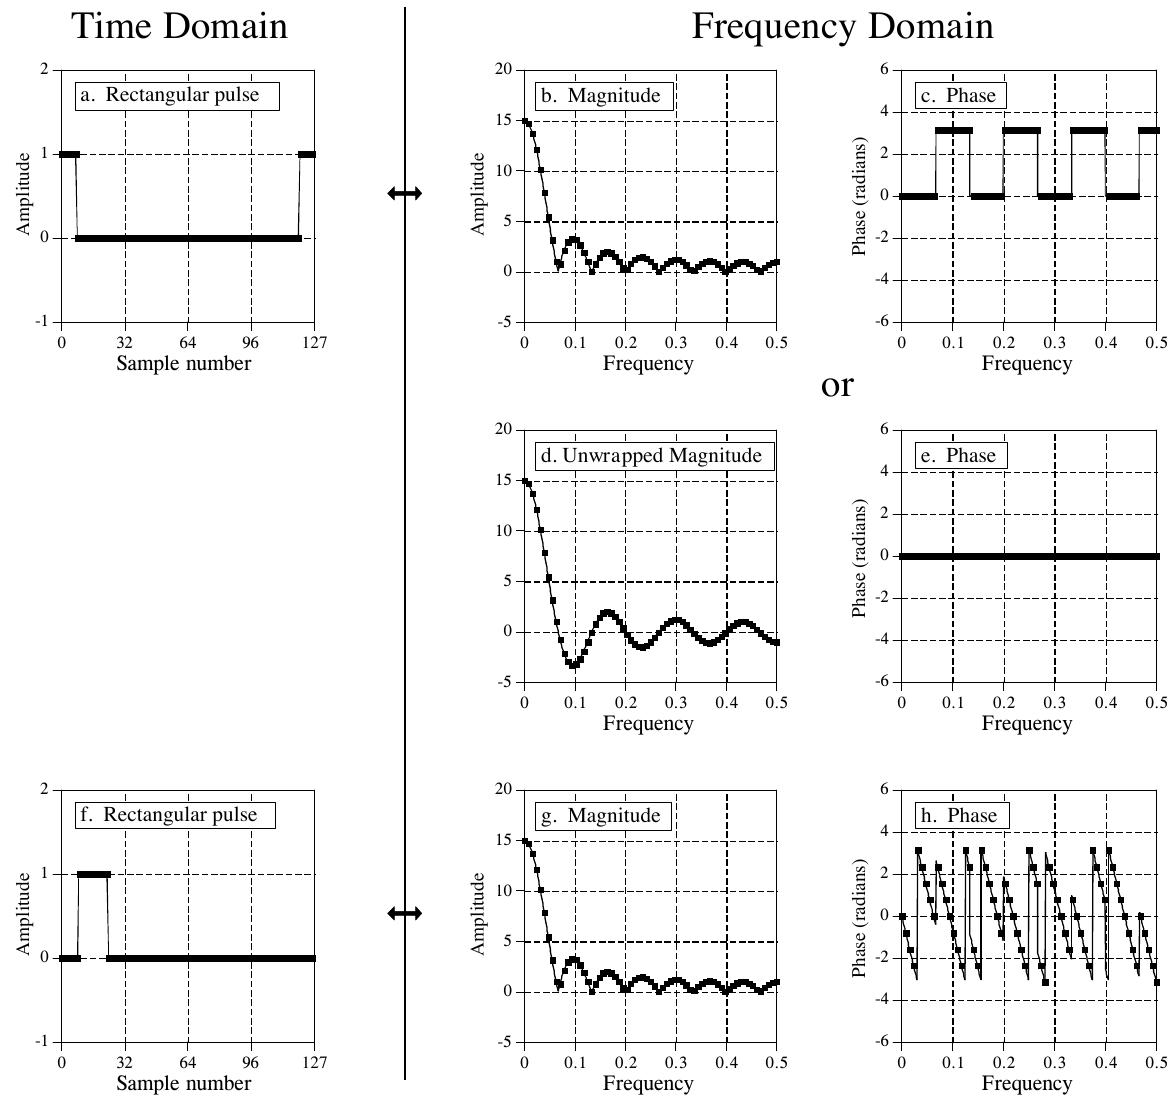
\includegraphics[width=0.979\linewidth,height=0.8\textheight,keepaspectratio]{assets/ch11/fig11-03.png}
\caption*{\textbf{图 11-3　矩形脉冲的 DFT。} 一个域中的矩形脉冲，对应另一个域中的
sinc 函数。 （Time Domain = 时域，Frequency Domain =
频域；a、f.~Rectangular pulse = 矩形脉冲；b、g. Magnitude =
幅度；c、e、h. Phase = 相位；d.~Unwrapped Magnitude = 展开幅度；中间的
or = 或者，表示 (b)(c) 与 (d)(e) 是同一频谱的两种表示。Amplitude =
幅度，Phase (radians) = 相位（弧度），Sample number =
采样序号，Frequency = 频率。）}
\end{figure}

另外，也可以用 DTFT 把频谱表示成采样率的分数 f 的函数：

\textbf{公式 11-2}　用采样频率改写的公式 11-1。参数 f 是采样率的分数，在
0 到 0.5 之间连续变化。为避免除以零，取 Mag X(0) = M。

\[\mathrm{Mag}\;X(f) = \left|\,\frac{\sin(\pi f M)}{\sin(\pi f)}\,\right|\]

（原书此公式的说明把 continuously 误拼成 continiously。）

换句话说，公式 11-1 给出频谱中的 N/2 + 1 个采样，而公式 11-2
给出这些采样所在的连续曲线。这两个公式只给出幅度。相位完全由时域波形的左右位置决定，上一章已经讨论过。

注意图 11-3b 中，振荡的幅度在频率到达 0.5
之前并没有衰减到零。你应该猜得到，这个波形会延续到下一个周期，在那里发生混叠(aliasing)。这改变了频域的形状，公式
11-1 和 11-2 已经把这种影响包括在内了。

了解没有混叠时频谱是什么样子，往往很重要。这是因为离散信号常常用来表示或模拟连续信号，而连续信号不会混叠。要去掉公式
11-1 和 11-2 中的混叠，只需把分母分别从 \(\sin(\pi k M/N)\) 改成
\(\pi k M/N\)、从 \(\sin(\pi f)\) 改成 \(\pi f\)。图 11-4
说明了这一改动的意义。由于 f 只能从 0 变到 0.5，πf 只能从 0 变到
1.5708。在这个范围内，\(\sin(\pi f)\) 和 \(\pi f\)
差别不大：在零频率处两者相等，在频率 0.5 处也只差约
36\%。如果没有混叠，图 11-3b
中的曲线在图的右侧会稍微低一点，在左侧则没有变化。

\begin{quote}
\textbf{译注：} 这里分母的写法照录原书。按公式 11-1、11-2
的形式，真正对应的分母是 \(\sin(\pi k/N)\) 和
\(\sin(\pi f)\)；原文第一处写成 \(\sin(\pi k M/N)\)（那是分子），应为
\(\sin(\pi k/N)\) 改成 \(\pi k/N\)。
\end{quote}

当矩形脉冲的频谱没有混叠时（因为时域信号是连续的，或者因为你忽略了混叠），它的一般形式是
\(\sin(x)/x\)，即 sinc 函数。对连续信号来说，矩形脉冲和 sinc
函数是傅里叶变换对；对离散信号来说这只是一种近似，误差来自混叠。

sinc 函数在 x = 0 处有一个恼人的问题：\(\sin(x)/x\)
变成了零除以零。这在数学上并不难办：当 x 变得非常小时，sin(x) 趋近于 x
的值（见图 11-4）。

\begin{figure}[htbp]
\centering
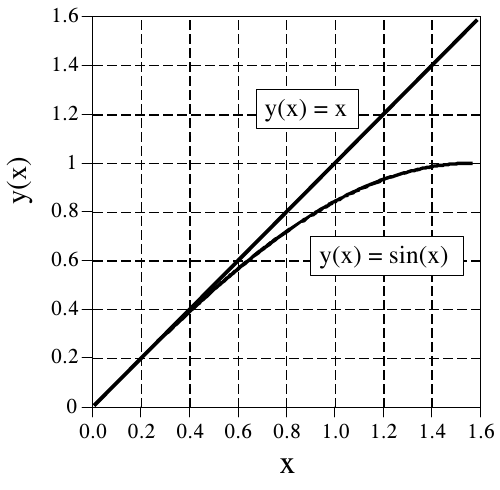
\includegraphics[width=0.417\linewidth,height=0.8\textheight,keepaspectratio]{assets/ch11/fig11-04.png}
\caption*{\textbf{图 11-4　x 与 sin(x) 的比较。} 函数 y(x) = x 和 y(x) = sin(x) 在
x 较小时很接近，在 1.57（π/2）处也只差约
36\%。这说明了混叠怎样使矩形脉冲的频谱偏离纯粹的 sinc 函数。
（图中两条曲线分别标注 y(x) = x 和 y(x) = sin(x)。）}
\end{figure}

这样 sinc 函数就变成了 x/x，其值为一。换句话说，当 x 越来越小时，sinc(x)
的值趋近于一，其中也包括 sinc(0) =
1。现在试着把这一点告诉你的计算机！它看到的只有除以零，于是会报错并让程序停下来。要记住的要点是：计算
sinc 函数时，程序必须对 x = 0 做特殊处理。

sinc
函数的一个关键特征是过零点的位置。它们出现在这样的频率上：正弦信号恰好有整数个周期能放进矩形脉冲里。例如，如果矩形脉冲宽
20 个点，频域中第一个零点位于''在 20
个点内完成一个完整周期''的频率处，第二个零点位于''在 20
个点内完成两个完整周期''的频率处，依此类推。回想 DFT
是怎样用相关计算的，就能理解这一点：一个频率分量的幅度，是把时域信号与一个正弦信号相乘、再把得到的采样加起来求得的。如果时域波形是一个幅度为
1
的矩形脉冲，这就等于把落在矩形脉冲内的那些正弦采样加起来。如果这个求和覆盖的是正弦信号的整数个周期，结果就是零。

sinc 函数在 DSP
中应用很广，因为它是一个非常简单的波形（矩形脉冲）的傅里叶变换对。例如，第
9 章讨论的频谱分析就用到了 sinc
函数。设想要分析一个无限长的离散信号。由于 DFT
只能处理有限长的信号，就选取 N
个采样来代表这个更长的信号。关键在于，``从长信号中选取 N
个采样''等同于把这个长信号乘以一个矩形脉冲：矩形脉冲中的 1
保留对应的采样，0
则把它们去掉。这对信号的频谱有什么影响呢？时域乘以一个矩形脉冲，导致频域与一个
sinc 函数卷积。这降低了频谱的分辨率，前面图 9-5a 已经展示过。

\section{其他变换对}

图 11-5 的 (a) 和 (b) 展示了上述内容的对偶：频域中的矩形脉冲对应时域中的
sinc 函数（加上混叠）。把混叠的影响包括在内，时域信号为：

\textbf{公式 11-3}　矩形脉冲的逆 DFT。在频域中，脉冲幅度为 1，从第 0
个采样一直到第 M−1 个采样。参数 N 是 DFT 的长度，x{[}i{]} 是时域信号，i
从 0 到 N−1。为避免除以零，取 x{[}0{]} = (2M−1)/N。

\[x[i] = \frac{1}{N}\,\frac{\sin\!\big(2\pi i\,(M - 1/2)/N\big)}{\sin(\pi i / N)}\]

要从这个公式中去掉混叠的影响，可以设想频域采样得无比精细，以至于变成一条连续曲线。这会使时域变成无限长、不再有周期性。这时该用的傅里叶变换是
DTFT，得到的时域信号由下面的关系给出：

\textbf{公式 11-4}　矩形脉冲的逆 DTFT。在频域中，脉冲幅度为
1，从零频率一直到截止频率 \(f_c\)，\(f_c\) 取 0 到 0.5
之间的值。时域信号存放在 x{[}i{]} 中，i 从 0 到 N−1。为避免除以零，取
x{[}0{]} = 2f\textsubscript{c}。

\[x[i] = \frac{\sin(2\pi f_c\, i)}{i\pi}\]

这个公式在 DSP
中非常重要，因为频域中的矩形脉冲就是理想的低通滤波器(perfect low-pass
filter)。因此，这个公式描述的 sinc
函数就是理想低通滤波器的滤波器核。这是一类非常有用的数字滤波器------加窗
sinc 滤波器(windowed-sinc filter)------的基础，第 15 章会介绍。

图 (c) 和 (d) 表明，时域中的三角形脉冲(triangular pulse)对应频域中的
sinc 平方（加上混叠）。这个变换对本身没有它成立的原因重要。一个 2M−1
点的三角形，可以由一个 M
点矩形脉冲与它自身卷积得到。由于时域卷积对应频域相乘，把一个波形与自身卷积，就会把它的频谱平方。

有没有一种波形，它的傅里叶变换就是它自己？答案是有，而且只有一种：高斯曲线(Gaussian)。图
(e) 是一条高斯曲线，(f)
是它对应的频谱，也是一条高斯曲线。只有忽略混叠时这个关系才成立。时域和频域标准差之间的关系为
\(2\pi\sigma_f = 1/\sigma_t\)。(f)
中只画出了高斯曲线的一侧，频谱中的负频率补全了整条曲线，对称中心在零频率处。

图 (g) 可以叫做高斯脉冲串(Gaussian
burst)。它由一个正弦波乘以一条高斯曲线构成。例如，(g) 就是一个正弦波乘以
(e)
中那条高斯曲线。对应的频域是一条中心不在零频率处的高斯曲线。和前面一样，这个变换对本身没有它成立的原因重要。由于时域信号是两个信号的乘积，频域就是这两个频谱的卷积。正弦波的频谱是位于该正弦波频率处的一个冲激函数；高斯曲线的频谱是以零频率为中心的一条高斯曲线。两者卷积，得到以正弦波频率为中心的一条高斯曲线。这应该看着眼熟：它和上一章介绍的调幅(amplitude
modulation)过程完全相同。

\begin{figure}[htbp]
\centering
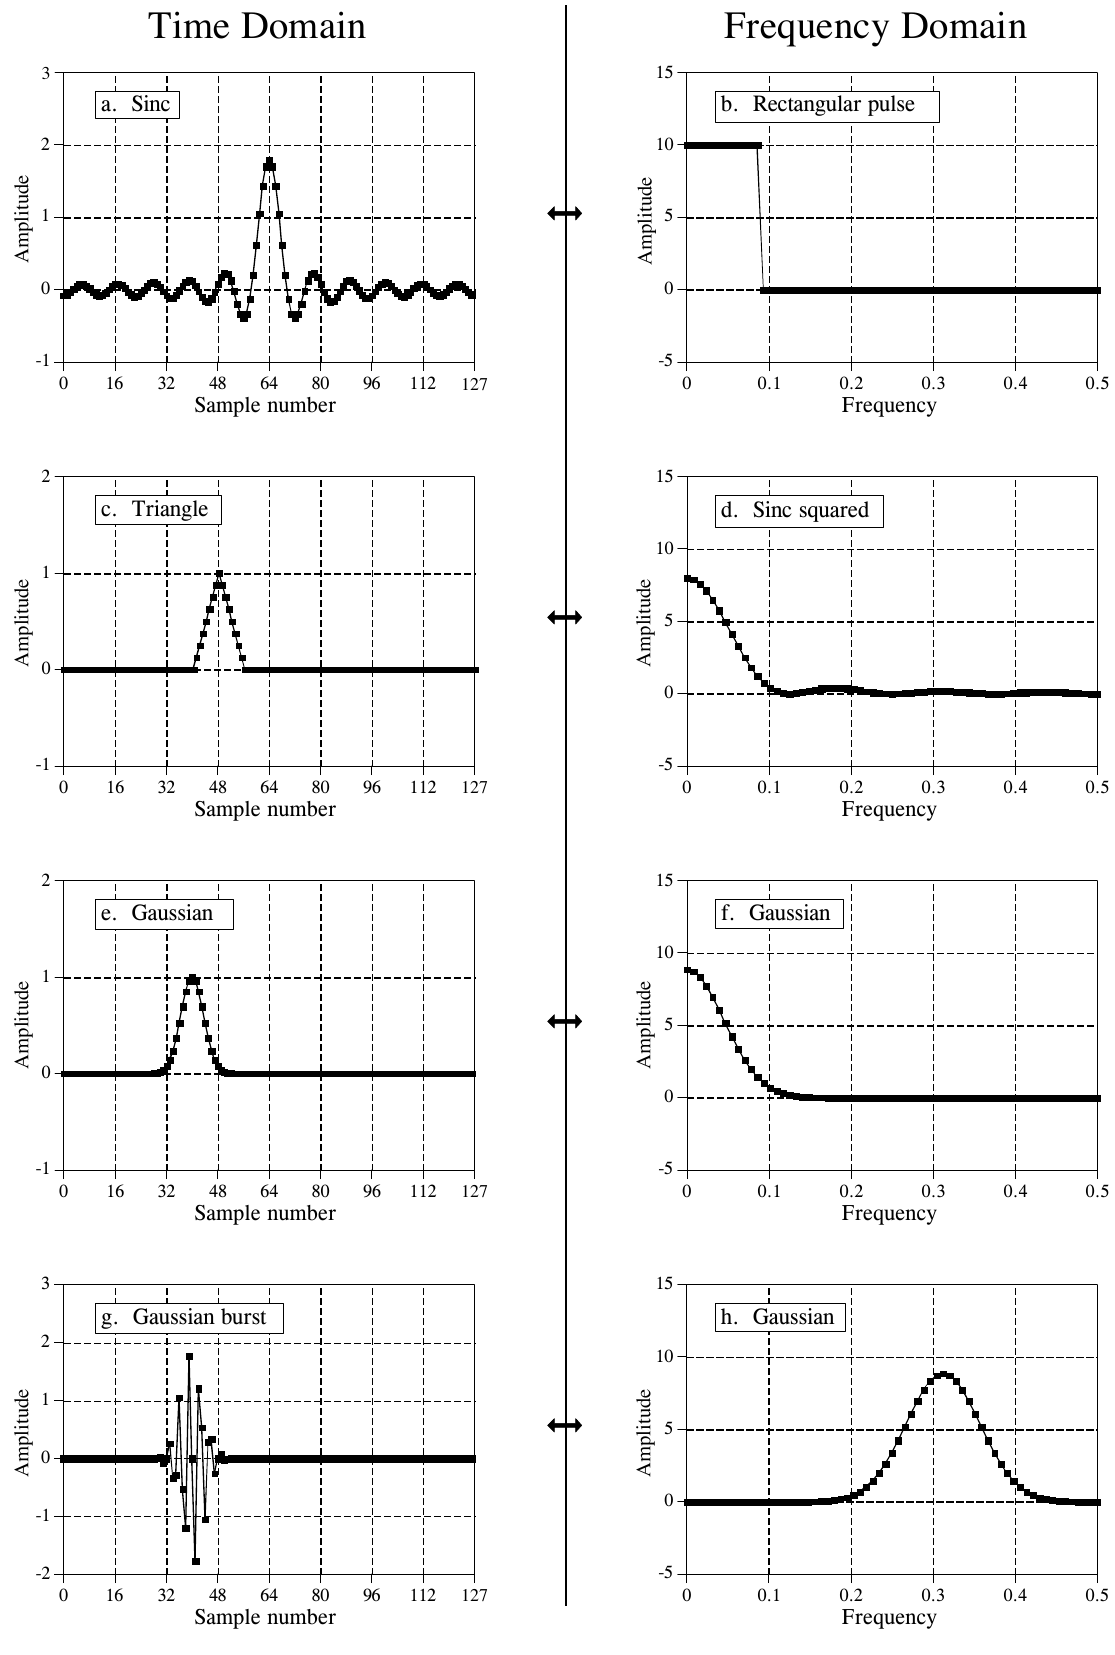
\includegraphics[width=0.929\linewidth,height=0.8\textheight,keepaspectratio]{assets/ch11/fig11-05.png}
\caption*{\textbf{图 11-5　常见的变换对。} （Time Domain = 时域，Frequency Domain
= 频域；a. Sinc = sinc 函数 \dspsym{↔} b. Rectangular pulse =
矩形脉冲；c.~Triangle = 三角形 \dspsym{↔} d.~Sinc squared = sinc
平方；e. Gaussian = 高斯曲线 \dspsym{↔} f.~Gaussian = 高斯曲线；g.
Gaussian burst = 高斯脉冲串 \dspsym{↔} h. Gaussian = 高斯曲线。Amplitude
= 幅度，Sample number = 采样序号，Frequency = 频率。）}
\end{figure}

\section{吉布斯效应}

图 11-6
展示了用正弦信号合成一个时域信号的过程。要重建的信号画在最后一幅图 (h)
中。这个信号长 1024 点，所以完整重建需要 513 个频率。图 (a) 到 (g)
展示了只用其中一部分频率时，重建出的信号是什么样子。例如，(f) 是用频率 0
到 100 重建的信号。它的做法是：对 (h) 中的信号做 DFT，把频率 101 到 512
设为零，再用逆 DFT 求出得到的时域信号。

重建中加入的频率越多，信号就越接近最终结果。有意思的是信号中的边沿处是怎样逼近最终结果的。(h)
中有三个陡峭的边沿：两个是矩形脉冲的边沿；第三个在第 1023 个采样和第 0
个采样之间，因为 DFT
把时域看作是周期性的。只用一部分频率重建时，每个边沿都会出现过冲(overshoot)和振铃（ringing，逐渐衰减的振荡）。这种过冲和振铃叫做吉布斯效应(Gibbs
effect)，以数学物理学家乔赛亚·吉布斯(Josiah Gibbs)的名字命名，他在 1899
年解释了这一现象。

仔细看 (e)、(f)、(g)
中的过冲。加入的正弦信号越多，过冲的宽度越窄；但过冲的幅度大致保持不变，约为
9\%。对离散信号来说这不成问题：加入最后一个频率时，过冲就消失了。然而，连续信号的重建就没那么好解释了。合成一个连续信号必须加入无穷多个正弦信号。问题在于，当正弦信号的个数趋于无穷时，过冲的幅度并不减小，而是保持在大约
9\%。鉴于这种情况（以及其他一些论点），人们有理由怀疑：连续正弦信号的求和到底能不能重建出一个边沿？还记得拉格朗日和傅里叶之间的那场争论吗？

解开这个谜题的关键在于：加入的正弦信号越多，过冲的宽度越小。正弦信号无穷多时过冲仍然存在，但宽度为零。恰好在间断点处，重建信号的值收敛到阶跃的中点。吉布斯证明，在''两者之间的误差能量为零''这个意义上，这个求和收敛到原信号。

与吉布斯效应有关的问题在 DSP
中经常遇到。例如，低通滤波器截掉了较高的频率，结果在时域的边沿处产生过冲和振铃。另一种常见的做法是截掉时域信号的两端，以免它们延伸到相邻的周期中去。根据对偶性，这会使频域中的边沿失真。这些问题会在后面讲滤波器设计的章节中再次出现。

\begin{figure}[htbp]
\centering
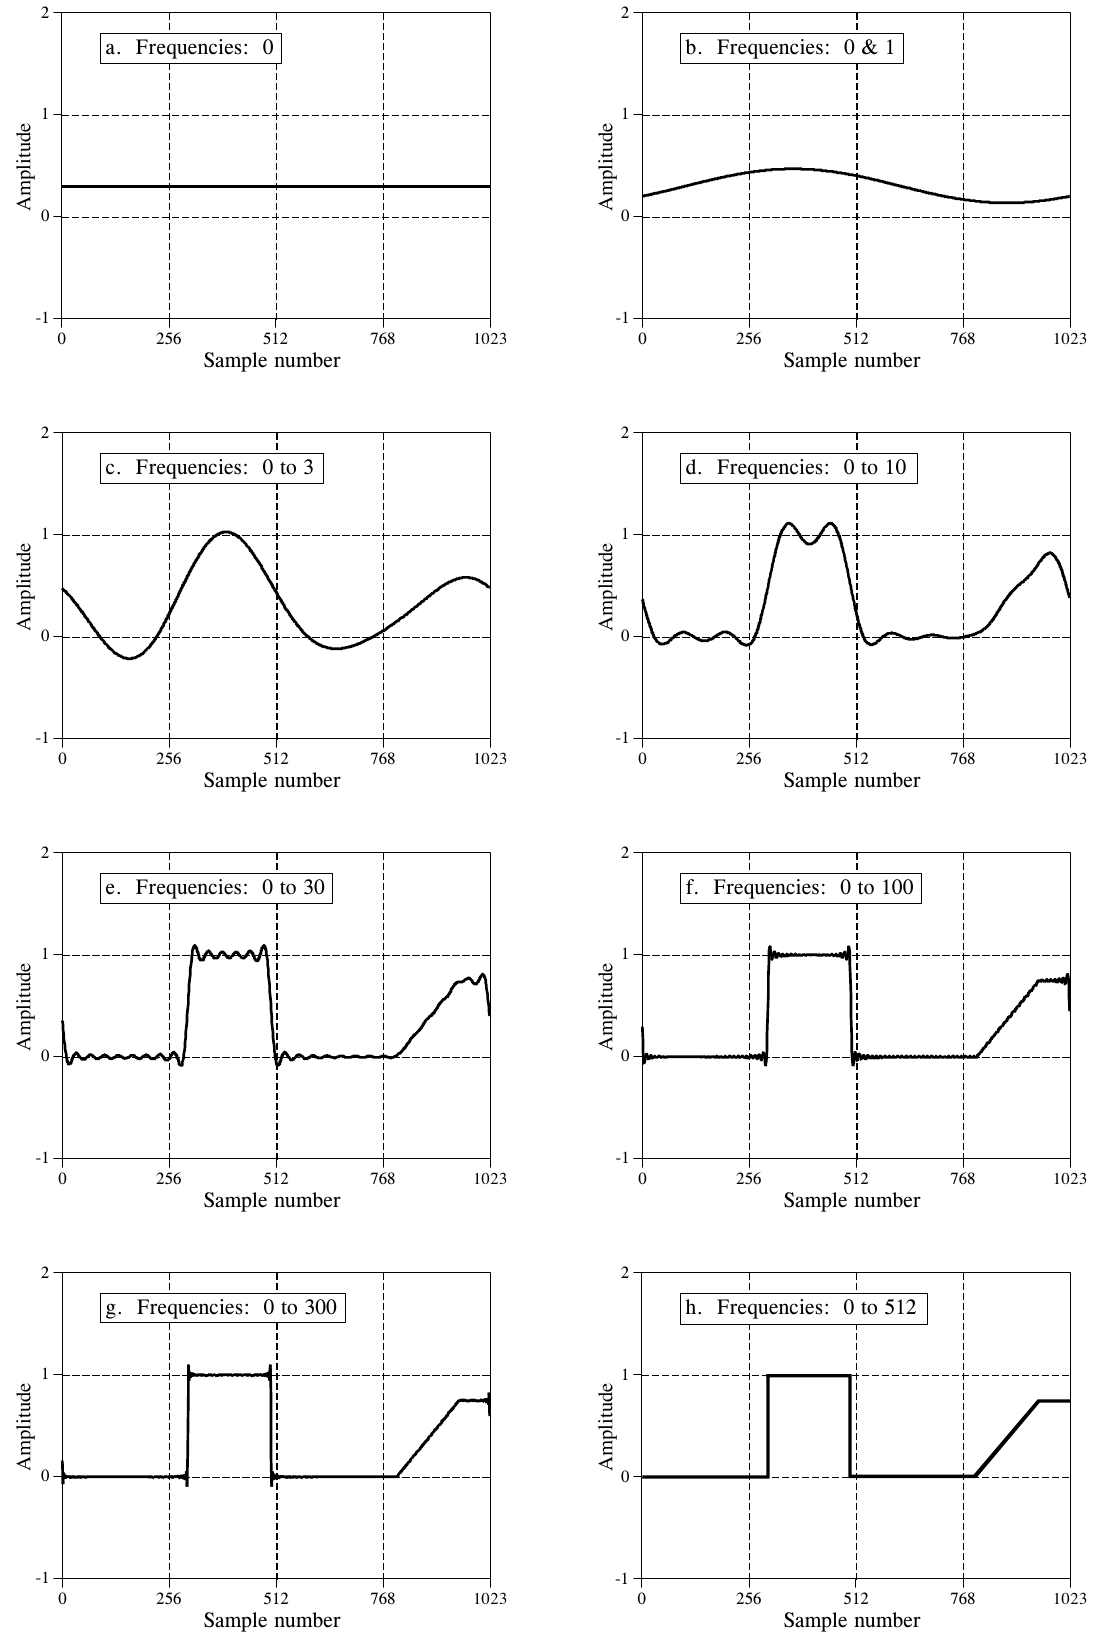
\includegraphics[width=0.917\linewidth,height=0.8\textheight,keepaspectratio]{assets/ch11/fig11-06.png}
\caption*{\textbf{图 11-6　吉布斯效应。} （a～h. Frequencies: 0 / 0 \& 1 / 0 to 3
/ 0 to 10 / 0 to 30 / 0 to 100 / 0 to 300 / 0 to 512 = 所用频率：0 / 0
和 1 / 0～3 / 0～10 / 0～30 / 0～100 / 0～300 / 0～512。Amplitude =
幅度，Sample number = 采样序号。）}
\end{figure}

\section{谐波}

如果一个信号以频率 f 呈周期性，那么组成这个信号的频率只有 f 的整数倍，即
f、2f、3f、4f 等。这些频率叫做谐波(harmonics)。一次谐波是 f，二次谐波是
2f，三次谐波是 3f，依此类推。一次谐波（即
f）还有一个专门的名字，叫基频(fundamental frequency)。图 11-7
是一个例子。图 (a) 是一个纯正弦波，(b) 是它的 DFT，只有一个峰。在 (c)
中，把正弦波的波峰顶部往里压，使正弦波发生失真。图 (d)
是这种失真在频域中的结果。由于失真后的信号仍以与原正弦波相同的频率呈周期性，频域由原来的峰加上若干谐波组成。谐波可以是任意幅度，不过通常随频率升高而变小。和任何信号一样，陡峭的边沿会带来更高的频率。例如，设想一个普通的
TTL 逻辑门产生 1 kHz 的方波。边沿在几纳秒内上升，会产生一直到将近 100
MHz 的谐波，也就是第一万次谐波！

\begin{figure}[htbp]
\centering
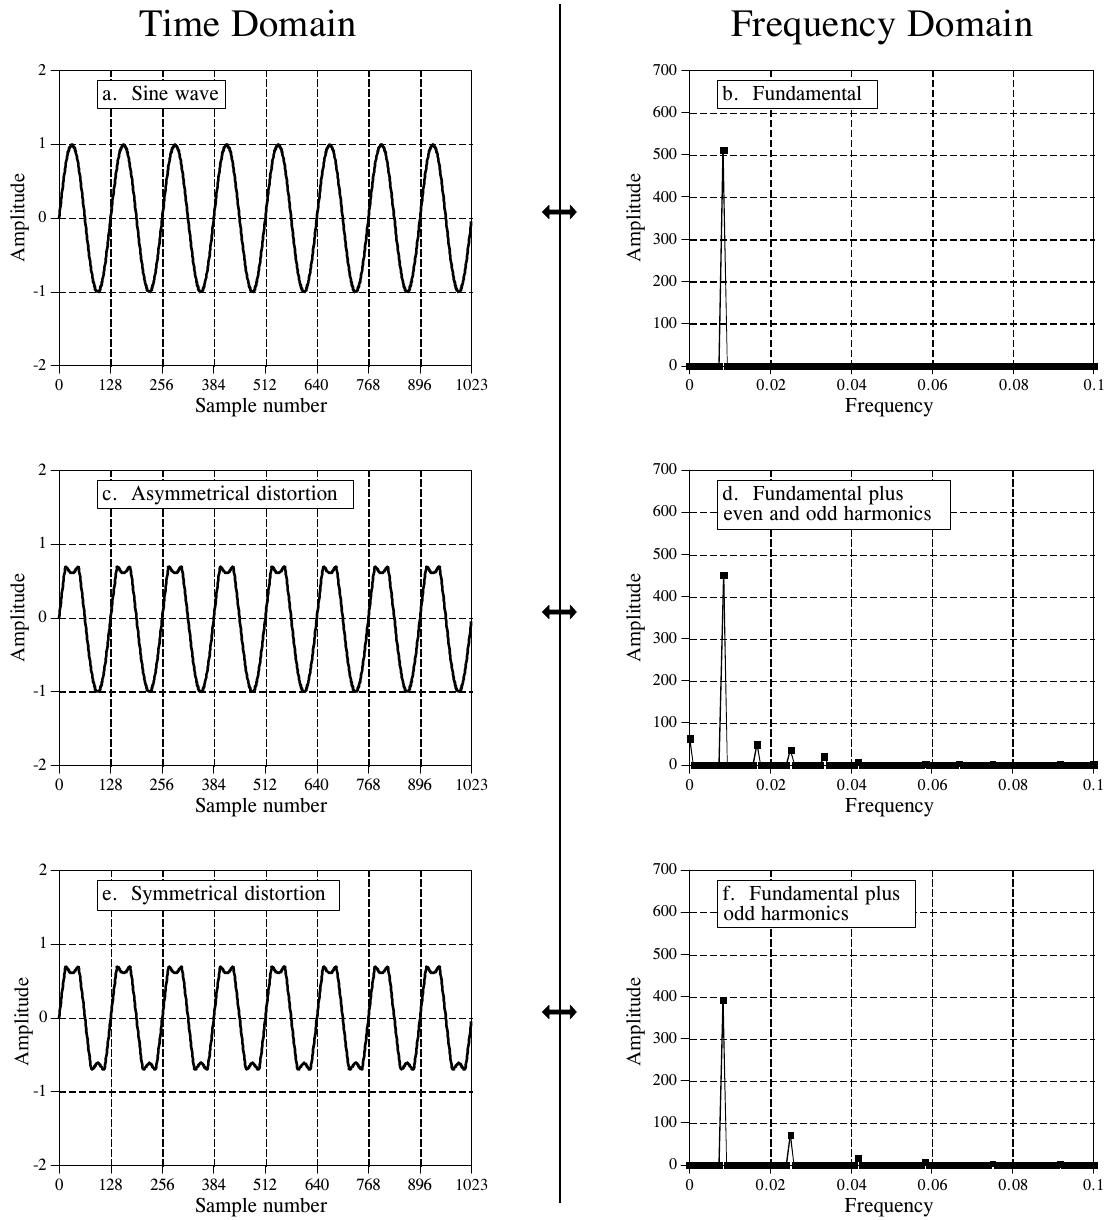
\includegraphics[width=0.925\linewidth,height=0.8\textheight,keepaspectratio]{assets/ch11/fig11-07.png}
\caption*{\textbf{图 11-7　谐波的例子。} (c) 中的不对称失真产生偶次和奇次谐波
(d)；而 (e) 中的对称失真只产生奇次谐波 (f)。 （Time Domain =
时域，Frequency Domain = 频域；a. Sine wave = 正弦波，b. Fundamental =
基波；c.~Asymmetrical distortion = 不对称失真，d.~Fundamental plus even
and odd harmonics = 基波加偶次和奇次谐波；e. Symmetrical distortion =
对称失真，f.~Fundamental plus odd harmonics = 基波加奇次谐波。Amplitude
= 幅度，Sample number = 采样序号，Frequency = 频率。）}
\end{figure}

\begin{quote}
\textbf{译注：} 原书图注写的是对称失真''只产生偶次谐波(only even
harmonics)``，与正文和图 (f)
的标注矛盾，应为''只产生奇次谐波''，这里按正确意思翻译。
\end{quote}

图 (e)
展示了谐波分析中的一个微妙之处。如果信号关于一条水平轴对称，即上半部分的波瓣是下半部分波瓣的镜像，那么所有偶次谐波的值都为零。如
(f) 所示，信号中只含有基波、三次谐波、五次谐波等。

所有连续的周期信号都可以像上面描述的那样，表示为谐波之和。离散的周期信号有一个问题，打乱了这种简单的关系。你大概已经猜到了，这个问题就是混叠。图
11-8a
是一个用同样方式（把波峰顶部往里压）失真了的正弦波。这个波形看起来远不如前一个例子那样规整平滑，因为这个正弦波的频率高得多，每个周期的采样点更少。图
(b)
是这个信号的频谱。不出所料，你能认出基波和谐波。这个例子表明，谐波可以延伸到高于采样频率
0.5 倍的频率上，并会混叠到 0 和 0.5 之间的某个频率。你在 (b)
中注意不到它们，因为它们的幅度太低。图 (c)
用对数刻度画出频谱，显示出这些低幅度的混叠峰。乍一看，这个频谱像随机噪声。其实不是，这是许多谐波混叠后相互重叠的结果。

\begin{figure}[htbp]
\centering
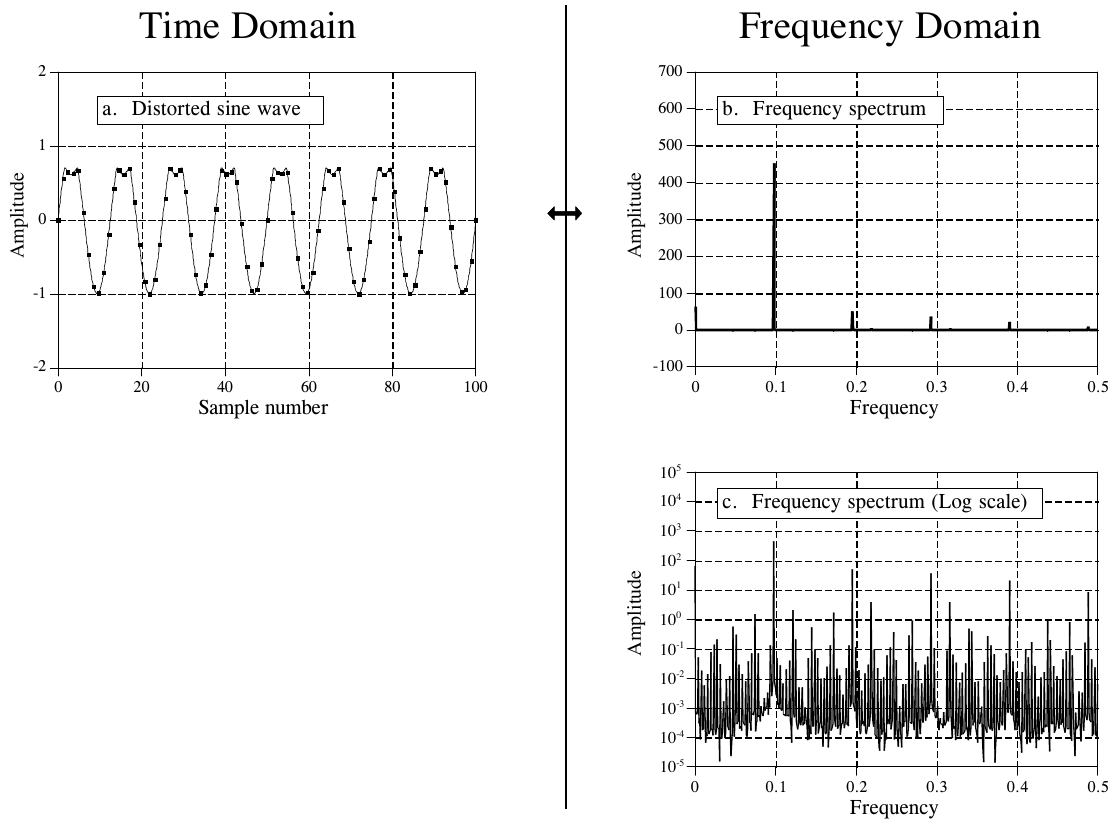
\includegraphics[width=0.929\linewidth,height=0.8\textheight,keepaspectratio]{assets/ch11/fig11-08.png}
\caption*{\textbf{图 11-8　谐波混叠。} 图 (a) 和 (b)
分别是一个失真的正弦波及其频谱。频率高于 0.5 的谐波会混叠到 0 和 0.5
之间的某个频率。图 (c)
用对数刻度画出同一频谱，显示出许多幅度很低的混叠峰。 （Time Domain =
时域，Frequency Domain = 频域；a. Distorted sine wave = 失真的正弦波；b.
Frequency spectrum = 频谱；c.~Frequency spectrum (Log scale) =
频谱（对数刻度）。Amplitude = 幅度，Sample number = 采样序号，Frequency
= 频率。原书图注说明排在左下方，裁图时已去掉，译文见上。）}
\end{figure}

要明白，这个例子是在信号已经数字化表示之后才使它失真的。如果这种失真发生在模拟信号中，你会在数字化之前用抗混叠滤波器(antialias
filter)去掉这些惹麻烦的谐波。只有直接对离散信号做非线性运算时，谐波混叠才是个问题。即便如此，这些混叠谐波的幅度也常常低到可以忽略。

谐波的概念还有另一个用处：它解释了为什么 DFT
把时域和频域都看作周期性的。在频域中，N 点 DFT 由 N/2+1
个等间距的频率组成。你可以把这些采样之间的频率看作 (1) 值为零，或者 (2)
不存在。不管哪种看法，它们都不参与时域信号的合成。换句话说，离散频谱由谐波组成，而不是由一段连续的频率范围组成。这就要求时域以频域中最低的正弦信号的频率（即基频）呈周期性。不计直流值，频域中表示的最低频率每
N 个采样完成一个完整周期，因此时域以 N
为周期呈周期性。换句话说，如果一个域是离散的，另一个域就必然是周期性的，反之亦然。这对傅里叶变换家族的四个成员都成立。由于
DFT
把两个域都看作离散的，它也必然把两个域都看作周期性的。每个域中的采样，代表的是另一个域的周期性所对应的谐波。

\section{啁啾信号}

啁啾信号(chirp
signal)是解决回声定位系统（如雷达和声呐）中一个实际问题的巧妙方法。图
11-9 是啁啾系统的频率响应。幅度恒为一，而相位是一条抛物线：

\textbf{公式 11-7}　啁啾系统的相位。

\[\mathrm{Phase}\;X[k] = \alpha k + \beta k^2\]

\begin{quote}
\textbf{译注：} 原书本章的公式编号从 11-4 直接跳到 11-7，没有 11-5 和
11-6，照原书保留。
\end{quote}

\begin{figure}[htbp]
\centering
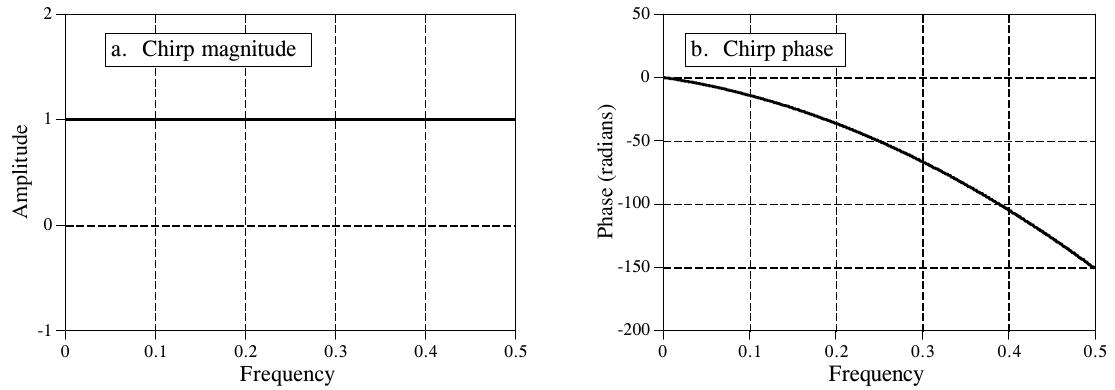
\includegraphics[width=0.929\linewidth,height=0.8\textheight,keepaspectratio]{assets/ch11/fig11-09.png}
\caption*{\textbf{图 11-9　啁啾系统的频率响应。} 幅度是常数，相位是一条抛物线。
（a. Chirp magnitude = 啁啾幅度；b. Chirp phase = 啁啾相位。Amplitude =
幅度，Phase (radians) = 相位（弧度），Frequency = 频率。）}
\end{figure}

参数 α
给相位引入一个线性斜率，也就是说，它只是按需要把冲激响应向左或向右平移。参数
β 控制相位的弯曲程度。这两个参数的选取必须使频率 0.5 处（即 k =
N/2）的相位是 2π 的整数倍。记住，只要直接修改相位，频率 0 和 0.5
处的相位都必须为零（或 2π 的整数倍，两者是一回事）。

图 11-10
展示了一个冲激进入啁啾系统，以及离开系统的冲激响应。冲激响应是一段振荡脉冲串，开始时频率低，随时间推移变成高频。它叫啁啾信号的原因很简单：用扬声器播放时，听起来像鸟的啁啾声。

\begin{figure}[htbp]
\centering
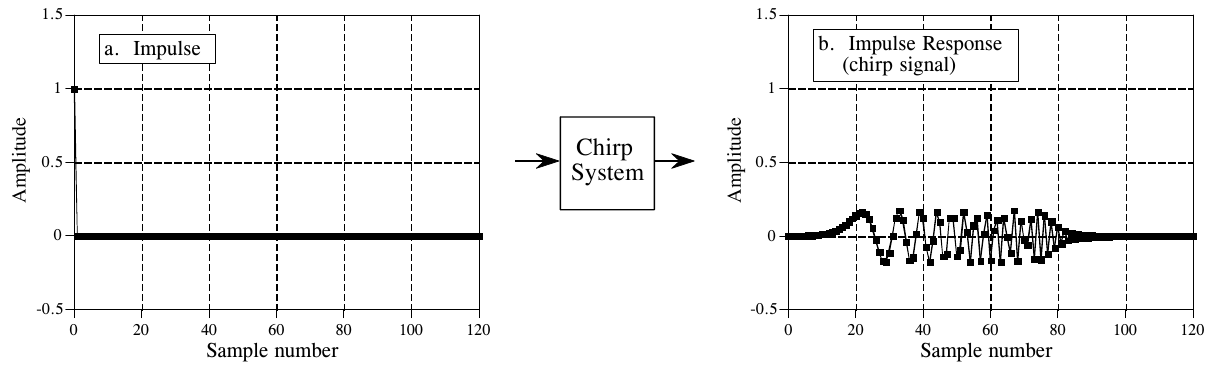
\includegraphics[width=1.000\linewidth,height=0.8\textheight,keepaspectratio]{assets/ch11/fig11-10.png}
\caption*{\textbf{图 11-10　啁啾系统。} 啁啾系统的冲激响应是一个啁啾信号。 （a.
Impulse = 冲激；b. Impulse Response (chirp signal) =
冲激响应（啁啾信号）；中间方框 Chirp System = 啁啾系统。Amplitude =
幅度，Sample number = 采样序号。）}
\end{figure}

啁啾系统的关键特点是它完全可逆。如果让啁啾信号通过一个反啁啾系统(antichirp
system)，信号又会变回一个冲激。这要求反啁啾系统的幅度为一，相位与啁啾系统相反。上一章讲过，这意味着反啁啾系统的冲激响应，可以通过把啁啾系统的冲激响应左右翻转得到。挺有意思，但它有什么用呢？

想想雷达系统是怎样工作的。一副定向天线发出一小段射频能量。飞机和其他物体把其中一部分能量反射回来，射向位于发射机旁边的无线电接收机。由于无线电波以恒定速度传播，发射信号与接收信号之间经过的时间就给出了到目标的距离。这引出了对脉冲的第一个要求：它要尽可能短。例如，1
微秒的脉冲产生的无线电波串约长 300
米。这意味着用这个系统得到的距离信息，分辨率也大约是这个长度。如果想要更好的距离分辨率，就需要更短的脉冲。

第二个要求很明显：如果想探测更远的物体，脉冲就需要更多的能量。不幸的是，更多的能量和更短的脉冲是相互矛盾的要求。产生一个脉冲所需的电功率，等于脉冲能量除以脉冲长度。既要更多能量又要更短脉冲，就使电功率的承受能力成为系统的限制因素。无线电发射机的输出级能承受的功率是有限的，超过了就会烧毁。

啁啾信号提供了一种打破这个限制的方法。在冲激到达无线电发射机的末级之前，先让它通过一个啁啾系统。这样从目标飞机上反弹回来的就不是一个冲激，而是一个啁啾信号。收到啁啾回波后，让信号通过一个反啁啾系统，把它还原成一个冲激。这使得系统中测量距离的部分看到的是短脉冲，而承受功率的电路看到的是持续时间长的信号。这种波形整形(waveshaping)是现代雷达系统的一个基本组成部分。

% !TEX root = ../main.tex
% 本文件由 build-tex.sh 从 12-DSP指南-第12章中译.md 生成，改内容请改 md 后重新生成

\chapter{快速傅里叶变换}\label{ch-12}

计算离散傅里叶变换（DFT）的方法有好几种，比如解联立线性方程组，或者第 8
章介绍的相关法。快速傅里叶变换（Fast Fourier Transform，FFT）是计算 DFT
的另一种方法。它得到的结果与其他方法相同，但效率高得惊人，计算时间常常能缩短几百倍。这就像坐喷气式飞机和走路的差别！如果没有
FFT，本书介绍的许多技术都没法实用。FFT 虽然只需要几十行代码，却是 DSP
中最复杂的算法之一。不过别泄气！你完全可以直接使用现成的 FFT
程序，而不必彻底弄懂它的内部原理。

\section{用复数 DFT 计算实数 DFT}

J.W. Cooley 和 J.W. Tukey 被公认为把 FFT
带给世界的人，他们的论文是：``An algorithm for the machine calculation
of complex Fourier
Series''（一种用机器计算复数傅里叶级数的算法），Mathematics
Computation，第 19 卷，1965 年，第 297～301
页。回头来看，其他人早在许多年前就发现了这一技术。例如，伟大的德国数学家卡尔·弗里德里希·高斯（1777--1855）一个多世纪以前就用过这种方法。这些早期工作基本被遗忘了，因为当时缺少让它变得实用的工具：数字计算机。Cooley
和 Tukey 之所以享有盛誉，是因为他们在正确的时间发现了
FFT------计算机革命的开端。

FFT 基于复数 DFT(complex DFT)，它是前四章讨论的实数 DFT(real DFT)
的一个更复杂的版本。这两种变换按各自表示数据的方式命名，也就是用复数还是用实数。``复数''(complex)
这个词并不是说这种表示方法困难或复杂，而是说它用到了一种特定的数学。复数数学确实常常困难又复杂，但名字不是从这儿来的。第
29 章讨论复数 DFT，并提供理解 FFT
算法细节所需的背景知识。本章的主题要简单些：怎样用 FFT 来计算实数
DFT，而不陷进高深数学的泥潭。

\begin{quote}
\textbf{译注：} 原书本章两处提到''第 29 章''讲复数 DFT，实际是第 31
章《复数傅里叶变换》（第 29 章是《DSP 上手实践》）。
\end{quote}

\begin{figure}[htbp]
\centering
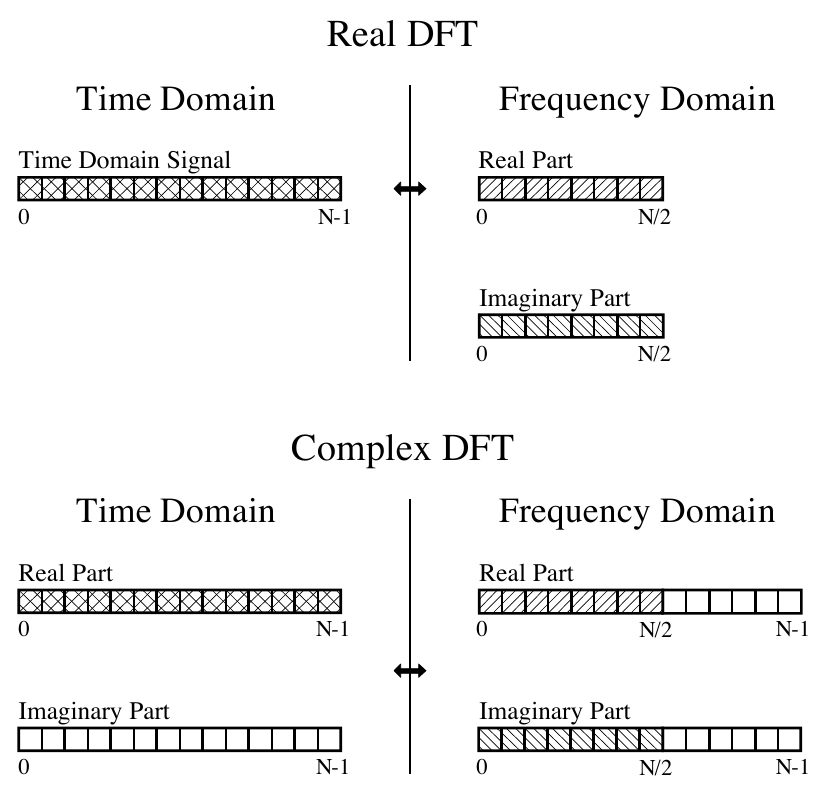
\includegraphics[width=0.688\linewidth,height=0.8\textheight,keepaspectratio]{assets/ch12/fig12-01.png}
\caption*{\textbf{图 12-1　实数 DFT 与复数 DFT 的比较。} 实数 DFT 把一个 N
点时域信号变成两个 N/2+1 点的频域信号。复数 DFT 把两个 N
点时域信号变成两个 N 点频域信号。画了斜线的区域表示两种变换共有的数值。
（Real DFT = 实数 DFT，Complex DFT = 复数 DFT；Time Domain =
时域，Frequency Domain = 频域；Time Domain Signal = 时域信号，Real Part
= 实部，Imaginary Part = 虚部。）}
\end{figure}

既然 FFT 是计算复数 DFT 的算法，弄清楚怎样把实数 DFT
的数据转入和转出复数 DFT 的格式就很重要。图 12-1 比较了实数 DFT 和复数
DFT 存放数据的方式。实数 DFT 把一个 N 点时域信号变换成两个 N/2+1
点的频域信号。这个时域信号就叫时域信号；频域中的两个信号分别叫实部(real
part)和虚部(imaginary
part)，存放余弦波和正弦波的幅度。这些在前几章都应该很熟悉了。

相比之下，复数 DFT 把两个 N 点时域信号变换成两个 N
点频域信号。两个时域信号也叫实部和虚部，和频域信号一样。尽管名字如此，这些数组中的所有值都只是普通的数。（如果你熟悉复数：数组值里不包含
j，j 是数学表达式的一部分。回忆一下，算子 Im( ) 返回的是一个实数。）

假设你有一个 N 点信号，需要借助复数 DFT（比如用 FFT 算法）来计算实数
DFT。首先，把这个 N 点信号放进复数 DFT
时域的实部，再把虚部的所有采样设为零。计算复数 DFT
后，频域得到一个实部信号和一个虚部信号，各有 N 个点。这两个信号的第
0～N/2 个采样，就对应实数 DFT 的频谱。

第 10 章讲过，把负频率包括进来时，DFT 的频域是周期性的（见图
10-9）。选哪一个周期是任意的，可以选 −1.0 到 0、−0.5 到 0.5、0 到
1.0，或者以采样率为参照的任何其他一个单位长的区间。复数 DFT 的频谱按 0
到 1.0 的方式包含负频率。也就是说，一个完整周期从第 0 个采样延伸到第 N−1
个采样，对应采样率的 0 到 1.0 倍。正频率位于第 0 到 N/2 个采样之间，对应
0 到 0.5。其余采样，即第 N/2+1 到 N−1 个，存放负频率的值（通常被忽略）。

用复数逆 DFT 计算实数逆 DFT
稍微难一点，因为你要保证负频率按正确的格式装入。记住，复数 DFT 的第
0～N/2 点与实数 DFT 相同，实部虚部都是如此。对于实部，第 N/2+1 点与第
N/2−1 点相同，第 N/2+2 点与第 N/2−2 点相同，依此类推，一直到第 N−1
点与第 1 点相同。虚部也是同样的基本模式，只是符号相反：第 N/2+1 点是第
N/2−1 点的相反数，第 N/2+2 点是第 N/2−2 点的相反数，等等。注意，第 0
点和第 N/2 点在这种复制模式中没有配对的点。可以参照图 10-9
来理解这种对称性。实际操作时，把实数 DFT 的频谱装入复数 DFT 数组的第
0～N/2 个采样，再用一个子程序生成第 N/2+1 到 N−1 个采样之间的负频率。表
12-1 就是这样一个程序。要检查对称性是否正确，可以在做完逆 FFT
后看时域的虚部：如果一切正确，它将全是零（用单精度计算时，会有百万分之几的噪声）。

\textbf{表 12-1}（注释已译成中文）

\begin{Shaded}
\begin{Highlighting}[]
\NormalTok{6000 \textquotesingle{}NEGATIVE FREQUENCY GENERATION}
\NormalTok{6010 \textquotesingle{}本子程序由实数频域生成复数频域。}
\NormalTok{6020 \textquotesingle{}进入本子程序时，N\% 是信号的点数，}
\NormalTok{6030 \textquotesingle{}REX[ ] 和 IMX[ ] 的第 0 到 N\%/2 个采样存放实数频域。}
\NormalTok{6040 \textquotesingle{}返回时，REX[ ] 和 IMX[ ] 的第 0 到 N\%{-}1 个采样存放复数频域。}
\NormalTok{6050 \textquotesingle{}}
\NormalTok{6060 FOR K\% = (N\%/2+1) TO (N\%{-}1)}
\NormalTok{6070 REX[K\%] = REX[N\%{-}K\%]}
\NormalTok{6080 IMX[K\%] = {-}IMX[N\%{-}K\%]}
\NormalTok{6090 NEXT K\%}
\NormalTok{6100 \textquotesingle{}}
\NormalTok{6110 RETURN}
\end{Highlighting}
\end{Shaded}

\textbf{C 实现}（完整可编译版本见
\texttt{c/table12-1\_negative\_freq.c}，其中用相关法复数 DFT
做对照，并按上文的方法检查逆变换后虚部是否为零）：

\begin{Shaded}
\begin{Highlighting}[]
\CommentTok{/* 6000：由实数频域生成复数频域。进入时 rex/imx 的 0～n/2 点有效，返回时 0～n{-}1 点都有效 */}
\DataTypeTok{static} \DataTypeTok{void}\NormalTok{ negative\_frequency\_generation}\OperatorTok{(}\DataTypeTok{double} \OperatorTok{*}\NormalTok{rex}\OperatorTok{,} \DataTypeTok{double} \OperatorTok{*}\NormalTok{imx}\OperatorTok{,} \DataTypeTok{int}\NormalTok{ n}\OperatorTok{)}
\OperatorTok{\{}
    \ControlFlowTok{for} \OperatorTok{(}\DataTypeTok{int}\NormalTok{ k }\OperatorTok{=}\NormalTok{ n }\OperatorTok{/} \DecValTok{2} \OperatorTok{+} \DecValTok{1}\OperatorTok{;}\NormalTok{ k }\OperatorTok{\textless{}=}\NormalTok{ n }\OperatorTok{{-}} \DecValTok{1}\OperatorTok{;}\NormalTok{ k}\OperatorTok{++)} \OperatorTok{\{}  \CommentTok{/* 6060：遍历负频率的每个点 */}
\NormalTok{        rex}\OperatorTok{[}\NormalTok{k}\OperatorTok{]} \OperatorTok{=}\NormalTok{ rex}\OperatorTok{[}\NormalTok{n }\OperatorTok{{-}}\NormalTok{ k}\OperatorTok{];}                    \CommentTok{/* 6070：实部偶对称 */}
\NormalTok{        imx}\OperatorTok{[}\NormalTok{k}\OperatorTok{]} \OperatorTok{=} \OperatorTok{{-}}\NormalTok{imx}\OperatorTok{[}\NormalTok{n }\OperatorTok{{-}}\NormalTok{ k}\OperatorTok{];}                   \CommentTok{/* 6080：虚部奇对称 */}
    \OperatorTok{\}}
\OperatorTok{\}}
\end{Highlighting}
\end{Shaded}

运行结果（N=64 随机实信号）：补出的负频率与完整频谱最大偏差 1.05e-13；逆
DFT 后时域虚部最大幅度 6.6e-15，实部与原信号最大偏差
1.3e-14。作为反例，不补负频率直接做逆变换，时域虚部最大幅度达到 0.44。

\section{FFT 的工作原理}

FFT 是一个复杂的算法，它的细节通常留给专门研究这类问题的人。本节介绍 FFT
的大致运作，但回避了一个关键问题：复数的使用。如果你有复数数学的背景，可以从字里行间读出这个算法的真正本质。细节看不明白也不用担心；在用
FFT 的科学家和工程师中，能从零写出这个程序的人寥寥无几。

在复数记法中，时域和频域各包含一个由 N
个复数点组成的信号。每个复数点由两个数组成：实部和虚部。例如，说到复数采样
X{[}42{]} 时，指的是 Re X{[}42{]} 和 Im X{[}42{]}
的组合。换句话说，每个复数变量存放两个数。两个复数变量相乘时，四个分量必须组合成乘积的两个分量（如公式
9-1）。下面关于''FFT
的工作原理''的讨论使用这种复数记法的行话。也就是说，单数的术语------信号、点、采样、值------都指实部和虚部的组合。

FFT 的工作方式是：把一个 N 点时域信号分解成 N
个时域信号，每个只含一个点。第二步，算出这 N 个时域信号对应的 N
个频谱。最后，把这 N 个频谱合成为一个频谱。

图 12-2 是 FFT 中所用时域分解的一个例子。本例中，一个 16
点信号经过四个独立的阶段分解。第一阶段把 16 点信号拆成两个各含 8
点的信号。第二阶段把数据分解成四个 4 点信号。这一模式一直继续，直到得到
N 个单点信号为止。每次把一个信号一分为二时，都用交错分解(interlaced
decomposition)，也就是把信号分成偶数号采样和奇数号采样。理解这一点最好的办法，是盯着图
12-2 看，直到你看出其中的规律。这种分解需要 \(\log_2 N\) 个阶段，例如 16
点信号（\(2^4\)）需要 4 个阶段，512 点信号（\(2^9\)）需要 9 个阶段，4096
点信号（\(2^{12}\)）需要 12 个阶段，等等。记住 \(\log_2 N\)
这个值，本章会多次提到它。

\begin{quote}
\textbf{译注：} 原书此处写''a 512 point signal (\(2^7\)) requires 7
stages''，有误：512 = \(2^9\)，需要 9 个阶段（\(2^7\) =
128）。译文已改正。
\end{quote}

\begin{figure}[htbp]
\centering
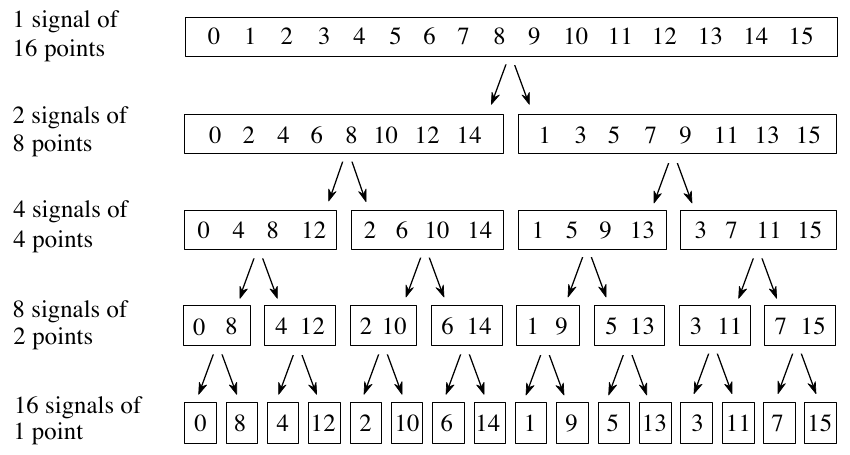
\includegraphics[width=0.708\linewidth,height=0.8\textheight,keepaspectratio]{assets/ch12/fig12-02.png}
\caption*{\textbf{图 12-2　FFT 的分解。} 一个 N 点信号被分解成 N
个各含一个点的信号。每个阶段都使用交错分解，把偶数号和奇数号采样分开。
（左侧从上到下：1 signal of 16 points = 1 个 16 点信号，2 signals of 8
points = 2 个 8 点信号，4 signals of 4 points = 4 个 4 点信号，8 signals
of 2 points = 8 个 2 点信号，16 signals of 1 point = 16 个 1 点信号。）}
\end{figure}

明白了分解的结构，就可以大大简化它。这种分解不过是把信号中的采样重新排序。图
12-3
给出了所需的重排规律。左边列出原信号的采样序号及其二进制形式；右边列出重排后的采样序号，也附上二进制形式。关键在于：左右两边的二进制数互为位反转。例如，第
3 个采样（0011）与第 12 个采样（1100）交换；同样，第 14
个采样（1110）与第 7 个采样（0111）交换，依此类推。FFT
的时域分解通常用位反转排序(bit reversal
sorting)算法完成，也就是把二进制数的位左右颠倒后计数，按这个顺序重排 N
个时域采样（就像图 12-3 最右一列那样）。

\begin{figure}[htbp]
\centering
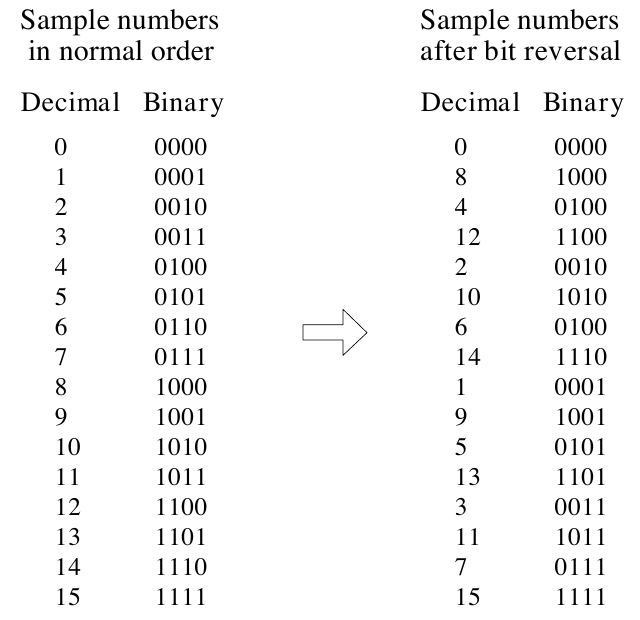
\includegraphics[width=0.533\linewidth,height=0.8\textheight,keepaspectratio]{assets/ch12/fig12-03.png}
\caption*{\textbf{图 12-3　FFT 的位反转排序。} FFT
的时域分解可以通过按位反转顺序给采样排序来实现。 （Sample numbers in
normal order = 正常顺序的采样序号，Sample numbers after bit reversal =
位反转后的采样序号；Decimal = 十进制，Binary = 二进制。原图右栏第 7
行十进制 6 的二进制印成了 0100，应为 0110。）}
\end{figure}

FFT 算法的下一步，是求这些 1 点时域信号的频谱。这再简单不过了：1
点信号的频谱就等于它自己。这意味着这一步什么都不用做。虽然不用做任何工作，别忘了：现在每个
1 点信号都是一个频谱，而不再是时域信号了。

FFT 的最后一步，是按与时域分解完全相反的顺序，把这 N
个频谱合并起来。算法从这里开始变得麻烦。可惜位反转这条捷径在这里用不上，我们必须一次退回一个阶段。在第一阶段，16
个频谱（每个 1 点）合成 8 个频谱（每个 2 点）。在第二阶段，8
个频谱（每个 2 点）合成 4 个频谱（每个 4
点），依此类推。最后一个阶段产生 FFT 的输出：一个 16 点频谱。

图 12-4 展示了两个各含 4 点的频谱怎样合并成一个 8
点频谱。这种合成必须撤销时域中所做的交错分解。换句话说，频域中的操作必须对应时域中''把两个
4 点信号交错合并''的过程。考虑两个时域信号 abcd 和
efgh。可以分两步得到一个 8 点时域信号：先在每个 4
点信号中插入零，把它稀释(dilute)成 8
点信号，然后把两个信号相加。也就是说，abcd 变成 a0b0c0d0，efgh 变成
0e0f0g0h，这两个 8 点信号相加得到 aebfcgdh。如图 12-4
所示，在时域中插零稀释，对应频谱的复制。因此，FFT
中合并频谱的方法，就是把它们复制一遍，再把复制后的频谱相加。

\begin{figure}[htbp]
\centering
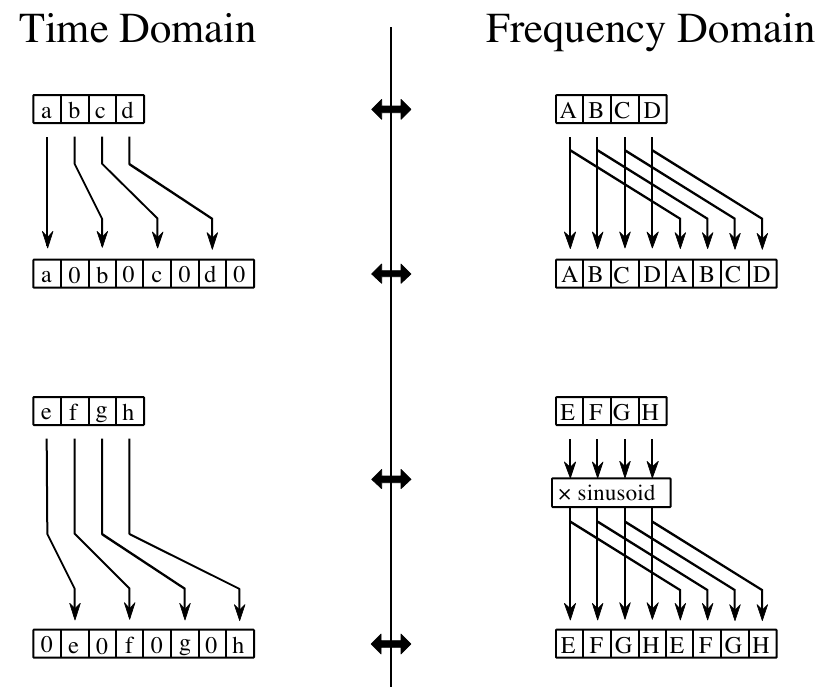
\includegraphics[width=0.692\linewidth,height=0.8\textheight,keepaspectratio]{assets/ch12/fig12-04.png}
\caption*{\textbf{图 12-4　FFT 的合成。}
时域信号插零稀释时，频域被复制一遍。如果稀释时时域信号还平移了一个采样，频谱还要再乘上一个正弦曲线。
（Time Domain = 时域，Frequency Domain = 频域，× sinusoid =
乘以正弦曲线。）}
\end{figure}

为了相加时能对上，两个时域信号的插零方式略有不同：一个信号的奇数点为零，另一个信号的偶数点为零。换句话说，其中一个时域信号（图
12-4 中的
0e0f0g0h）向右平移了一个采样。时域的这个平移，对应频谱乘上一个正弦曲线(sinusoid)。要看清这一点，回忆一下：时域中的平移等价于把信号与一个平移过的冲激函数卷积，这相当于把信号的频谱乘以平移冲激函数的频谱，而平移冲激函数的频谱是一条正弦曲线（见图
11-2）。

\begin{figure}[htbp]
\centering
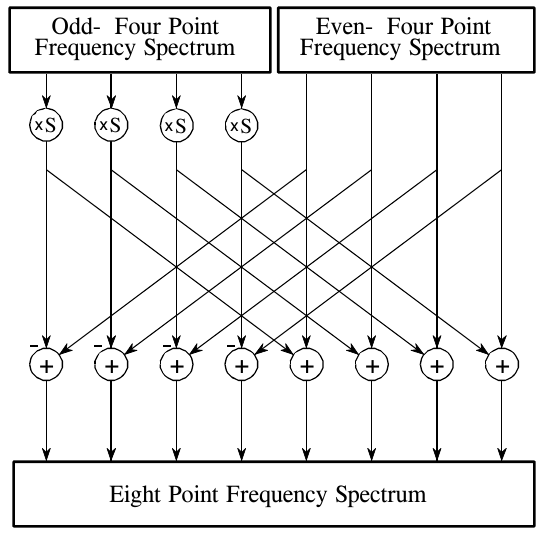
\includegraphics[width=0.458\linewidth,height=0.8\textheight,keepaspectratio]{assets/ch12/fig12-05.png}
\caption*{\textbf{图 12-5　FFT 合成流程图。} 这里展示了把两个 4 点频谱合并成一个 8
点频谱的方法。×S 运算表示把信号乘以一个频率选取得当的正弦曲线。 （Odd-
Four Point Frequency Spectrum = 奇数点的 4 点频谱，Even- Four Point
Frequency Spectrum = 偶数点的 4 点频谱，Eight Point Frequency Spectrum =
8 点频谱；加号旁的 − 表示该路相减。）}
\end{figure}

图 12-5 是把两个 4 点频谱合并成一个 8
点频谱的流程图。再进一步简化：注意图 12-5 是由图 12-6
中的基本模式一再重复构成的。这个简单的流程图因为形似翅膀而被称为蝶形(butterfly)。蝶形是
FFT 的基本计算单元，它把两个复数点变换成另外两个复数点。

\begin{figure}[htbp]
\centering
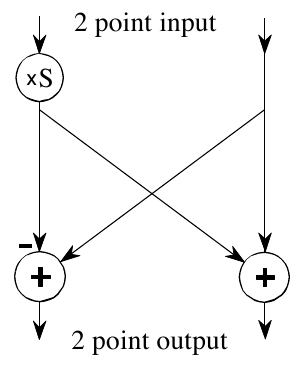
\includegraphics[width=0.254\linewidth,height=0.8\textheight,keepaspectratio]{assets/ch12/fig12-06.png}
\caption*{\textbf{图 12-6　FFT 蝶形。} 这是 FFT
的基本计算单元，取两个复数点，把它们变换成另外两个复数点。 （2 point
input = 2 点输入，2 point output = 2 点输出，×S = 乘以正弦曲线。）}
\end{figure}

图 12-7 展示了整个 FFT
的结构。时域分解由位反转排序算法完成。把分解后的数据变换到频域不需要做任何事，所以图中没有出现这一步。

频域合成需要三重循环。外层循环遍历 \(\log_2 N\) 个阶段（即图 12-2
中的每一层，从下往上）。中层循环遍历当前阶段中的每个频谱（即图 12-2
中任意一层上的每个方框）。最内层循环用蝶形计算每个频谱中的各个点（即遍历图
12-2 中任意一个方框里的采样）。图 12-7
中的''开销''(overhead)方框负责确定循环的起止下标，并计算蝶形所需的正弦曲线。现在我们来到本章的核心：实际的
FFT 程序。

\begin{figure}[htbp]
\centering
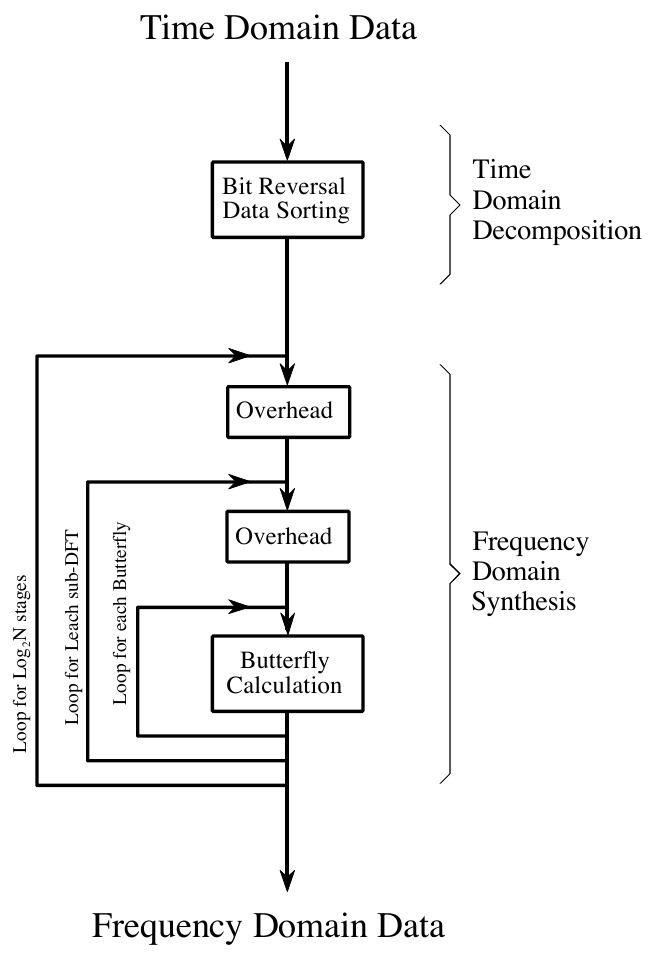
\includegraphics[width=0.546\linewidth,height=0.8\textheight,keepaspectratio]{assets/ch12/fig12-07.png}
\caption*{\textbf{图 12-7　FFT 流程图。} 它基于三个步骤：(1) 把一个 N
点时域信号分解成 N 个各含一个点的信号；(2) 求这 N
个点信号各自的频谱（什么都不用做）；(3) 把这 N 个频谱合成为一个频谱。
（Time Domain Data = 时域数据，Bit Reversal Data Sorting =
位反转数据排序，Time Domain Decomposition = 时域分解；Overhead =
开销（准备循环下标和正弦值），Butterfly Calculation =
蝶形计算，Frequency Domain Synthesis = 频域合成，Frequency Domain Data =
频域数据。三个循环从外到内：Loop for Log₂N stages = 遍历 log₂N
个阶段，Loop for each sub-DFT = 遍历每个子 DFT（原图误印为 Leach），Loop
for each Butterfly = 遍历每个蝶形。）}
\end{figure}

\section{FFT 程序}

第 8 章讲过，实数 DFT
可以通过把时域信号与正弦波和余弦波做相关来计算（见表 8-2）。表 12-2
给出了用同样的方法计算复数 DFT 的程序。公平对比的话，FFT
改进的正是这个程序。

\textbf{表 12-2}（注释已译成中文）

\begin{Shaded}
\begin{Highlighting}[]
\NormalTok{5000 \textquotesingle{}COMPLEX DFT BY CORRELATION}
\NormalTok{5010 \textquotesingle{}进入时，N\% 是 DFT 的点数，}
\NormalTok{5020 \textquotesingle{}XR[ ] 和 XI[ ] 是时域的实部和虚部。}
\NormalTok{5030 \textquotesingle{}返回时，REX[ ] 和 IMX[ ] 存放频域数据。}
\NormalTok{5040 \textquotesingle{}所有信号都从 0 到 N\%{-}1。}
\NormalTok{5050 \textquotesingle{}}
\NormalTok{5060 PI = 3.14159265                           \textquotesingle{}设置常数}
\NormalTok{5070 \textquotesingle{}}
\NormalTok{5080 FOR K\% = 0 TO N\%{-}1                        \textquotesingle{}把 REX[ ] 和 IMX[ ] 清零，}
\NormalTok{5090 REX[K\%] = 0                               \textquotesingle{}以便相关时当累加器用}
\NormalTok{5100 IMX[K\%] = 0}
\NormalTok{5110 NEXT K\%}
\NormalTok{5120 \textquotesingle{}}
\NormalTok{5130 FOR K\% = 0 TO N\%{-}1                        \textquotesingle{}遍历频域的每个值}
\NormalTok{5140 FOR I\% = 0 TO N\%{-}1                        \textquotesingle{}与复正弦 SR 和 SI 做相关}
\NormalTok{5150 \textquotesingle{}}
\NormalTok{5160 SR = COS(2*PI*K\%*I\%/N\%)                   \textquotesingle{}计算复正弦}
\NormalTok{5170 SI = {-}SIN(2*PI*K\%*I\%/N\%)}
\NormalTok{5180 REX[K\%] = REX[K\%] + XR[I\%]*SR {-} XI[I\%]*SI}
\NormalTok{5190 IMX[K\%] = IMX[K\%] + XR[I\%]*SI + XI[I\%]*SR}
\NormalTok{5200 \textquotesingle{}}
\NormalTok{5210 NEXT I\%}
\NormalTok{5220 NEXT K\%}
\NormalTok{5230 \textquotesingle{}}
\NormalTok{5240 RETURN}
\end{Highlighting}
\end{Shaded}

\textbf{C 实现}（完整可编译版本见
\texttt{c/table12-2\_complex\_dft\_correlation.c}）：

\begin{Shaded}
\begin{Highlighting}[]
\CommentTok{/* 5000：相关法复数 DFT。xr/xi 是时域，rex/imx 是频域，下标都是 0～n{-}1 */}
\DataTypeTok{static} \DataTypeTok{void}\NormalTok{ complex\_dft}\OperatorTok{(}\DataTypeTok{const} \DataTypeTok{double} \OperatorTok{*}\NormalTok{xr}\OperatorTok{,} \DataTypeTok{const} \DataTypeTok{double} \OperatorTok{*}\NormalTok{xi}\OperatorTok{,} \DataTypeTok{int}\NormalTok{ n}\OperatorTok{,} \DataTypeTok{double} \OperatorTok{*}\NormalTok{rex}\OperatorTok{,} \DataTypeTok{double} \OperatorTok{*}\NormalTok{imx}\OperatorTok{)}
\OperatorTok{\{}
    \ControlFlowTok{for} \OperatorTok{(}\DataTypeTok{int}\NormalTok{ k }\OperatorTok{=} \DecValTok{0}\OperatorTok{;}\NormalTok{ k }\OperatorTok{\textless{}}\NormalTok{ n}\OperatorTok{;}\NormalTok{ k}\OperatorTok{++)} \OperatorTok{\{}           \CommentTok{/* 5080～5110：REX[]、IMX[] 清零，相关时当累加器用 */}
\NormalTok{        rex}\OperatorTok{[}\NormalTok{k}\OperatorTok{]} \OperatorTok{=} \FloatTok{0.0}\OperatorTok{;}
\NormalTok{        imx}\OperatorTok{[}\NormalTok{k}\OperatorTok{]} \OperatorTok{=} \FloatTok{0.0}\OperatorTok{;}
    \OperatorTok{\}}
    \ControlFlowTok{for} \OperatorTok{(}\DataTypeTok{int}\NormalTok{ k }\OperatorTok{=} \DecValTok{0}\OperatorTok{;}\NormalTok{ k }\OperatorTok{\textless{}}\NormalTok{ n}\OperatorTok{;}\NormalTok{ k}\OperatorTok{++)}             \CommentTok{/* 5130：遍历频域的每个点 */}
        \ControlFlowTok{for} \OperatorTok{(}\DataTypeTok{int}\NormalTok{ i }\OperatorTok{=} \DecValTok{0}\OperatorTok{;}\NormalTok{ i }\OperatorTok{\textless{}}\NormalTok{ n}\OperatorTok{;}\NormalTok{ i}\OperatorTok{++)} \OperatorTok{\{}       \CommentTok{/* 5140：与复正弦 SR、SI 做相关 */}
            \DataTypeTok{double}\NormalTok{ sr }\OperatorTok{=}\NormalTok{ cos}\OperatorTok{(}\FloatTok{2.0} \OperatorTok{*}\NormalTok{ PI }\OperatorTok{*}\NormalTok{ k }\OperatorTok{*}\NormalTok{ i }\OperatorTok{/}\NormalTok{ n}\OperatorTok{);}      \CommentTok{/* 5160～5170：算出复正弦 */}
            \DataTypeTok{double}\NormalTok{ si }\OperatorTok{=} \OperatorTok{{-}}\NormalTok{sin}\OperatorTok{(}\FloatTok{2.0} \OperatorTok{*}\NormalTok{ PI }\OperatorTok{*}\NormalTok{ k }\OperatorTok{*}\NormalTok{ i }\OperatorTok{/}\NormalTok{ n}\OperatorTok{);}
\NormalTok{            rex}\OperatorTok{[}\NormalTok{k}\OperatorTok{]} \OperatorTok{+=}\NormalTok{ xr}\OperatorTok{[}\NormalTok{i}\OperatorTok{]} \OperatorTok{*}\NormalTok{ sr }\OperatorTok{{-}}\NormalTok{ xi}\OperatorTok{[}\NormalTok{i}\OperatorTok{]} \OperatorTok{*}\NormalTok{ si}\OperatorTok{;}          \CommentTok{/* 5180～5190：复数乘法后累加 */}
\NormalTok{            imx}\OperatorTok{[}\NormalTok{k}\OperatorTok{]} \OperatorTok{+=}\NormalTok{ xr}\OperatorTok{[}\NormalTok{i}\OperatorTok{]} \OperatorTok{*}\NormalTok{ si }\OperatorTok{+}\NormalTok{ xi}\OperatorTok{[}\NormalTok{i}\OperatorTok{]} \OperatorTok{*}\NormalTok{ sr}\OperatorTok{;}
        \OperatorTok{\}}
\OperatorTok{\}}
\end{Highlighting}
\end{Shaded}

运行结果（N=64）：冲激的频谱处处为 1+0j（偏差为 0）；频率为 5
的复正弦只在 X{[}5{]} 处得到 64，其余点幅度不超过
1.1e-13；实信号的频谱满足''实部偶对称、虚部奇对称''，偏差 1.0e-13。

表 12-3 和表 12-4 是两个不同的 FFT 程序，一个用 FORTRAN 写，一个用 BASIC
写。先看表 12-4 的 BASIC 子程序。它产生的输出与表 12-2
的相关法完全相同，只是快得多。可以用图 12-7
的方框图来辨认这个程序的各个部分。数据通过数组 REX{[} {]} 和 IMX{[} {]}
传给这个 FFT 子程序，下标都从 0 到 N−1。从子程序返回时，REX{[} {]} 和
IMX{[} {]} 被频域数据覆盖。这是 FFT
高度优化的又一个体现：输入、中间存储和输出都用同一组数组。这种高效的内存使用，对设计计算
FFT 的高速硬件很重要。描述这种内存用法的术语叫原地计算(in-place
computation)。

所有 FFT 程序得到的数值结果都一样，但在编程上有些细微差别需要留意。表
12-3 的 FORTRAN
程序体现了其中几种差别。这个程序使用一种叫按频率抽取(decimation in
frequency)的算法，而前面介绍的算法叫按时间抽取(decimation in
time)。在按频率抽取的算法中，位反转排序放在三重嵌套循环之后进行。还有一些
FFT 程序完全省掉了位反转排序。这些变体都不能显著提高 FFT
的性能，你不必操心用的是哪一种。

FFT 算法之间重要的差别，在于数据怎样传入和传出子程序。在 BASIC
程序中，数据通过数组 REX{[} {]} 和 IMX{[} {]} 进出子程序，采样下标从 0
到 N−1。在 FORTRAN 程序中，数据通过复数数组 X( ) 传递，采样下标从 1 到
N。由于这是一个复数变量数组，X( )
中的每个采样都由两个数组成：实部和虚部。DFT
的长度也必须传给这些子程序。BASIC 程序用变量 N\% 来传；相比之下，FORTRAN
程序用变量 M，它定义为 \(\log_2 N\)。例如，256 点 DFT 的 M 是 8，4096 点
DFT 的 M 是 12，等等。要点是，写 FFT
子程序的程序员在怎样与主程序对接方面有很多选择。像 FORTRAN 程序这样从 1
到 N 的数组尤其让人恼火。大多数 DSP 文献（包括本书）都假定数组从第 0
到第 N−1 个采样来讲解算法。例如，如果数组从 1 到 N，频域的对称中心就是第
1 点和第 N/2+1 点，而不是第 0 点和第 N/2 点。

\textbf{表 12-3　用 FORTRAN 写的快速傅里叶变换。} 数据通过变量 X( ) 和 M
传给这个子程序。整数 M 是 DFT 长度的以 2 为底的对数，例如 256 点 DFT 的
M = 8，4096 点 DFT 的 M = 12，等等。复数数组 X( )
在进入时存放时域数据，从子程序返回时被频域数据覆盖。注意：这个子程序要求输入和输出信号从
X(1) 到 X(N)，而不是通常的 X(0) 到 X(N−1)。

\begin{Shaded}
\begin{Highlighting}[]
      \KeywordTok{SUBROUTINE}\NormalTok{ FFT(X,M)}
      \DataTypeTok{COMPLEX}\NormalTok{ X(}\DecValTok{4096}\NormalTok{),U,S,T}
\NormalTok{      PI}\KeywordTok{=}\FloatTok{3.14159265}
\NormalTok{      N}\KeywordTok{=}\DecValTok{2}\KeywordTok{**}\NormalTok{M}
      \KeywordTok{DO} \DecValTok{20}\NormalTok{ L}\KeywordTok{=}\DecValTok{1}\NormalTok{,M}
\NormalTok{      LE}\KeywordTok{=}\DecValTok{2}\KeywordTok{**}\NormalTok{(M}\KeywordTok{+}\DecValTok{1}\KeywordTok{{-}}\NormalTok{L)}
\NormalTok{      LE2}\KeywordTok{=}\NormalTok{LE}\KeywordTok{/}\DecValTok{2}
\NormalTok{      U}\KeywordTok{=}\NormalTok{(}\FloatTok{1.0}\NormalTok{,}\FloatTok{0.0}\NormalTok{)}
\NormalTok{      S}\KeywordTok{=}\BuiltInTok{CMPLX}\NormalTok{(}\BuiltInTok{COS}\NormalTok{(PI}\KeywordTok{/}\BuiltInTok{FLOAT}\NormalTok{(LE2)),}\KeywordTok{{-}}\BuiltInTok{SIN}\NormalTok{(PI}\KeywordTok{/}\BuiltInTok{FLOAT}\NormalTok{(LE2)))}
      \KeywordTok{DO} \DecValTok{20}\NormalTok{ J}\KeywordTok{=}\DecValTok{1}\NormalTok{,LE2}
      \KeywordTok{DO} \DecValTok{10}\NormalTok{ I}\KeywordTok{=}\NormalTok{J,N,LE}
\NormalTok{      IP}\KeywordTok{=}\NormalTok{I}\KeywordTok{+}\NormalTok{LE2}
\NormalTok{      T}\KeywordTok{=}\NormalTok{X(I)}\KeywordTok{+}\NormalTok{X(IP)}
\NormalTok{      X(IP)}\KeywordTok{=}\NormalTok{(X(I)}\KeywordTok{{-}}\NormalTok{X(IP))}\KeywordTok{*}\NormalTok{U}
 \DecValTok{10}\NormalTok{   X(I)}\KeywordTok{=}\NormalTok{T}
 \DecValTok{20}\NormalTok{   U}\KeywordTok{=}\NormalTok{U}\KeywordTok{*}\NormalTok{S}
\NormalTok{      ND2}\KeywordTok{=}\NormalTok{N}\KeywordTok{/}\DecValTok{2}
\NormalTok{      NM1}\KeywordTok{=}\NormalTok{N}\KeywordTok{{-}}\DecValTok{1}
\NormalTok{      J}\KeywordTok{=}\DecValTok{1}
      \KeywordTok{DO} \DecValTok{50}\NormalTok{ I}\KeywordTok{=}\DecValTok{1}\NormalTok{,NM1}
      \KeywordTok{IF}\NormalTok{(I}\OperatorTok{.GE.}\NormalTok{J) }\KeywordTok{GO} \KeywordTok{TO} \DecValTok{30}
\NormalTok{      T}\KeywordTok{=}\NormalTok{X(J)}
\NormalTok{      X(J)}\KeywordTok{=}\NormalTok{X(I)}
\NormalTok{      X(I)}\KeywordTok{=}\NormalTok{T}
 \DecValTok{30}\NormalTok{   K}\KeywordTok{=}\NormalTok{ND2}
 \DecValTok{40}   \KeywordTok{IF}\NormalTok{(K}\OperatorTok{.GE.}\NormalTok{J) }\KeywordTok{GO} \KeywordTok{TO} \DecValTok{50}
\NormalTok{      J}\KeywordTok{=}\NormalTok{J}\KeywordTok{{-}}\NormalTok{K}
\NormalTok{      K}\KeywordTok{=}\NormalTok{K}\KeywordTok{/}\DecValTok{2}
      \KeywordTok{GO} \KeywordTok{TO} \DecValTok{40}
 \DecValTok{50}\NormalTok{   J}\KeywordTok{=}\NormalTok{J}\KeywordTok{+}\NormalTok{K}
      \KeywordTok{RETURN}
      \KeywordTok{END}
\end{Highlighting}
\end{Shaded}

\textbf{C 实现}（完整可编译版本见
\texttt{c/table12-3\_fft\_fortran.c}。为了逐行对照，C 版本同样用从 1
开始的下标，复数用 C99 的 \texttt{double\ complex}）：

\begin{Shaded}
\begin{Highlighting}[]
\CommentTok{/* SUBROUTINE FFT(X,M)：x[1]～x[n] 进为时域、出为频域 */}
\DataTypeTok{static} \DataTypeTok{void}\NormalTok{ fft\_fortran}\OperatorTok{(}\DataTypeTok{double} \DataTypeTok{complex} \OperatorTok{*}\NormalTok{x}\OperatorTok{,} \DataTypeTok{int}\NormalTok{ m}\OperatorTok{)}
\OperatorTok{\{}
    \DataTypeTok{int}\NormalTok{ n }\OperatorTok{=} \DecValTok{1} \OperatorTok{\textless{}\textless{}}\NormalTok{ m}\OperatorTok{;}                                         \CommentTok{/* N=2**M */}
    \ControlFlowTok{for} \OperatorTok{(}\DataTypeTok{int}\NormalTok{ l }\OperatorTok{=} \DecValTok{1}\OperatorTok{;}\NormalTok{ l }\OperatorTok{\textless{}=}\NormalTok{ m}\OperatorTok{;}\NormalTok{ l}\OperatorTok{++)} \OperatorTok{\{}                          \CommentTok{/* DO 20 L=1,M：遍历每一级 */}
        \DataTypeTok{int}\NormalTok{ le }\OperatorTok{=} \DecValTok{1} \OperatorTok{\textless{}\textless{}} \OperatorTok{(}\NormalTok{m }\OperatorTok{+} \DecValTok{1} \OperatorTok{{-}}\NormalTok{ l}\OperatorTok{);}                          \CommentTok{/* LE=2**(M+1{-}L)：本级子 DFT 的长度，从 N 开始逐级减半 */}
        \DataTypeTok{int}\NormalTok{ le2 }\OperatorTok{=}\NormalTok{ le }\OperatorTok{/} \DecValTok{2}\OperatorTok{;}
        \DataTypeTok{double} \DataTypeTok{complex}\NormalTok{ u }\OperatorTok{=} \FloatTok{1.0}\OperatorTok{;}                             \CommentTok{/* U=(1.0,0.0) */}
        \DataTypeTok{double} \DataTypeTok{complex}\NormalTok{ s }\OperatorTok{=}\NormalTok{ cos}\OperatorTok{(}\NormalTok{PI }\OperatorTok{/}\NormalTok{ le2}\OperatorTok{)} \OperatorTok{{-}}\NormalTok{ I }\OperatorTok{*}\NormalTok{ sin}\OperatorTok{(}\NormalTok{PI }\OperatorTok{/}\NormalTok{ le2}\OperatorTok{);}   \CommentTok{/* S=CMPLX(COS(PI/LE2),{-}SIN(PI/LE2)) */}
        \ControlFlowTok{for} \OperatorTok{(}\DataTypeTok{int}\NormalTok{ j }\OperatorTok{=} \DecValTok{1}\OperatorTok{;}\NormalTok{ j }\OperatorTok{\textless{}=}\NormalTok{ le2}\OperatorTok{;}\NormalTok{ j}\OperatorTok{++)} \OperatorTok{\{}                    \CommentTok{/* DO 20 J=1,LE2 */}
            \ControlFlowTok{for} \OperatorTok{(}\DataTypeTok{int}\NormalTok{ i }\OperatorTok{=}\NormalTok{ j}\OperatorTok{;}\NormalTok{ i }\OperatorTok{\textless{}=}\NormalTok{ n}\OperatorTok{;}\NormalTok{ i }\OperatorTok{+=}\NormalTok{ le}\OperatorTok{)} \OperatorTok{\{}              \CommentTok{/* DO 10 I=J,N,LE：遍历每个蝶形 */}
                \DataTypeTok{int}\NormalTok{ ip }\OperatorTok{=}\NormalTok{ i }\OperatorTok{+}\NormalTok{ le2}\OperatorTok{;}
                \DataTypeTok{double} \DataTypeTok{complex}\NormalTok{ t }\OperatorTok{=}\NormalTok{ x}\OperatorTok{[}\NormalTok{i}\OperatorTok{]} \OperatorTok{+}\NormalTok{ x}\OperatorTok{[}\NormalTok{ip}\OperatorTok{];}            \CommentTok{/* T=X(I)+X(IP) */}
\NormalTok{                x}\OperatorTok{[}\NormalTok{ip}\OperatorTok{]} \OperatorTok{=} \OperatorTok{(}\NormalTok{x}\OperatorTok{[}\NormalTok{i}\OperatorTok{]} \OperatorTok{{-}}\NormalTok{ x}\OperatorTok{[}\NormalTok{ip}\OperatorTok{])} \OperatorTok{*}\NormalTok{ u}\OperatorTok{;}                 \CommentTok{/* X(IP)=(X(I){-}X(IP))*U：先相减再乘正弦，与按时间抽取的蝶形相反 */}
\NormalTok{                x}\OperatorTok{[}\NormalTok{i}\OperatorTok{]} \OperatorTok{=}\NormalTok{ t}\OperatorTok{;}                                   \CommentTok{/* 10 X(I)=T */}
            \OperatorTok{\}}
\NormalTok{            u }\OperatorTok{=}\NormalTok{ u }\OperatorTok{*}\NormalTok{ s}\OperatorTok{;}                                      \CommentTok{/* 20 U=U*S：标号 20 属于 J 循环，每个 J 转一次 */}
        \OperatorTok{\}}
    \OperatorTok{\}}

    \DataTypeTok{int}\NormalTok{ nd2 }\OperatorTok{=}\NormalTok{ n }\OperatorTok{/} \DecValTok{2}\OperatorTok{,}\NormalTok{ nm1 }\OperatorTok{=}\NormalTok{ n }\OperatorTok{{-}} \DecValTok{1}\OperatorTok{,}\NormalTok{ j }\OperatorTok{=} \DecValTok{1}\OperatorTok{;}                    \CommentTok{/* ND2=N/2，NM1=N{-}1，J=1 */}
    \ControlFlowTok{for} \OperatorTok{(}\DataTypeTok{int}\NormalTok{ i }\OperatorTok{=} \DecValTok{1}\OperatorTok{;}\NormalTok{ i }\OperatorTok{\textless{}=}\NormalTok{ nm1}\OperatorTok{;}\NormalTok{ i}\OperatorTok{++)} \OperatorTok{\{}                        \CommentTok{/* DO 50 I=1,NM1：位反转排序 */}
        \ControlFlowTok{if} \OperatorTok{(}\NormalTok{i }\OperatorTok{\textless{}}\NormalTok{ j}\OperatorTok{)} \OperatorTok{\{}                                        \CommentTok{/* IF(I.GE.J) GO TO 30 */}
            \DataTypeTok{double} \DataTypeTok{complex}\NormalTok{ t }\OperatorTok{=}\NormalTok{ x}\OperatorTok{[}\NormalTok{j}\OperatorTok{];}
\NormalTok{            x}\OperatorTok{[}\NormalTok{j}\OperatorTok{]} \OperatorTok{=}\NormalTok{ x}\OperatorTok{[}\NormalTok{i}\OperatorTok{];}
\NormalTok{            x}\OperatorTok{[}\NormalTok{i}\OperatorTok{]} \OperatorTok{=}\NormalTok{ t}\OperatorTok{;}
        \OperatorTok{\}}
        \DataTypeTok{int}\NormalTok{ k }\OperatorTok{=}\NormalTok{ nd2}\OperatorTok{;}                                        \CommentTok{/* 30 K=ND2 */}
        \ControlFlowTok{while} \OperatorTok{(}\NormalTok{k }\OperatorTok{\textless{}}\NormalTok{ j}\OperatorTok{)} \OperatorTok{\{}                                     \CommentTok{/* 40 IF(K.GE.J) GO TO 50 */}
\NormalTok{            j }\OperatorTok{{-}=}\NormalTok{ k}\OperatorTok{;}                                         \CommentTok{/* J=J{-}K */}
\NormalTok{            k }\OperatorTok{/=} \DecValTok{2}\OperatorTok{;}                                         \CommentTok{/* K=K/2，GO TO 40 */}
        \OperatorTok{\}}
\NormalTok{        j }\OperatorTok{+=}\NormalTok{ k}\OperatorTok{;}                                             \CommentTok{/* 50 J=J+K */}
    \OperatorTok{\}}
\OperatorTok{\}}
\end{Highlighting}
\end{Shaded}

运行结果：随机复信号与相关法复数 DFT 逐点比较，最大偏差 N=8 时
1.9e-15，N=64 时 1.4e-13，N=1024 时 1.0e-11。

\textbf{表 12-4　用 BASIC 写的快速傅里叶变换。}（注释已译成中文）

\begin{Shaded}
\begin{Highlighting}[]
\NormalTok{1000 \textquotesingle{}THE FAST FOURIER TRANSFORM}
\NormalTok{1010 \textquotesingle{}进入时，N\% 是 DFT 的点数，REX[ ] 和}
\NormalTok{1020 \textquotesingle{}IMX[ ] 是输入的实部和虚部。返回时，}
\NormalTok{1030 \textquotesingle{}REX[ ] 和 IMX[ ] 存放 DFT 的输出。所有信号都从 0 到 N\%{-}1。}
\NormalTok{1040 \textquotesingle{}}
\NormalTok{1050 PI = 3.14159265                                    \textquotesingle{}设置常数}
\NormalTok{1060 NM1\% = N\%{-}1}
\NormalTok{1070 ND2\% = N\%/2}
\NormalTok{1080 M\% = CINT(LOG(N\%)/LOG(2))}
\NormalTok{1090 J\% = ND2\%}
\NormalTok{1100 \textquotesingle{}}
\NormalTok{1110 FOR I\% = 1 TO N\%{-}2                                 \textquotesingle{}位反转排序}
\NormalTok{1120 IF I\% \textgreater{}= J\% THEN GOTO 1190}
\NormalTok{1130 TR = REX[J\%]}
\NormalTok{1140 TI = IMX[J\%]}
\NormalTok{1150 REX[J\%] = REX[I\%]}
\NormalTok{1160 IMX[J\%] = IMX[I\%]}
\NormalTok{1170 REX[I\%] = TR}
\NormalTok{1180 IMX[I\%] = TI}
\NormalTok{1190 K\% = ND2\%}
\NormalTok{1200 IF K\% \textgreater{} J\% THEN GOTO 1240}
\NormalTok{1210 J\% = J\%{-}K\%}
\NormalTok{1220 K\% = K\%/2}
\NormalTok{1230 GOTO 1200}
\NormalTok{1240 J\% = J\%+K\%}
\NormalTok{1250 NEXT I\%}
\NormalTok{1260 \textquotesingle{}}
\NormalTok{1270 FOR L\% = 1 TO M\%                                   \textquotesingle{}遍历每一级}
\NormalTok{1280 LE\% = CINT(2\^{}L\%)}
\NormalTok{1290 LE2\% = LE\%/2}
\NormalTok{1300 UR = 1}
\NormalTok{1310 UI = 0}
\NormalTok{1320 SR = COS(PI/LE2\%)                                  \textquotesingle{}计算正弦和余弦值}
\NormalTok{1330 SI = {-}SIN(PI/LE2\%)}
\NormalTok{1340 FOR J\% = 1 TO LE2\%                                 \textquotesingle{}遍历每个子 DFT}
\NormalTok{1350 JM1\% = J\%{-}1}
\NormalTok{1360 FOR I\% = JM1\% TO NM1\% STEP LE\%                     \textquotesingle{}遍历每个蝶形}
\NormalTok{1370     IP\% = I\%+LE2\%}
\NormalTok{1380     TR = REX[IP\%]*UR {-} IMX[IP\%]*UI                 \textquotesingle{}蝶形计算}
\NormalTok{1390     TI = REX[IP\%]*UI + IMX[IP\%]*UR}
\NormalTok{1400     REX[IP\%] = REX[I\%]{-}TR}
\NormalTok{1410     IMX[IP\%] = IMX[I\%]{-}TI}
\NormalTok{1420     REX[I\%] = REX[I\%]+TR}
\NormalTok{1430     IMX[I\%] = IMX[I\%]+TI}
\NormalTok{1440 NEXT I\%}
\NormalTok{1450 TR = UR}
\NormalTok{1460 UR = TR*SR {-} UI*SI}
\NormalTok{1470 UI = TR*SI + UI*SR}
\NormalTok{1480 NEXT J\%}
\NormalTok{1490 NEXT L\%}
\NormalTok{1500 \textquotesingle{}}
\NormalTok{1510 RETURN}
\end{Highlighting}
\end{Shaded}

\textbf{C 实现}（完整可编译版本见 \texttt{c/table12-4\_fft.c}）：

\begin{Shaded}
\begin{Highlighting}[]
\CommentTok{/* 1110～1250：位反转排序 */}
\DataTypeTok{static} \DataTypeTok{void}\NormalTok{ bit\_reversal\_sort}\OperatorTok{(}\DataTypeTok{double} \OperatorTok{*}\NormalTok{rex}\OperatorTok{,} \DataTypeTok{double} \OperatorTok{*}\NormalTok{imx}\OperatorTok{,} \DataTypeTok{int}\NormalTok{ n}\OperatorTok{)}
\OperatorTok{\{}
    \DataTypeTok{int}\NormalTok{ nd2 }\OperatorTok{=}\NormalTok{ n }\OperatorTok{/} \DecValTok{2}\OperatorTok{,}\NormalTok{ j }\OperatorTok{=}\NormalTok{ nd2}\OperatorTok{;}                   \CommentTok{/* 1070、1090：ND2\% = N\%/2，J\% = ND2\% */}
    \ControlFlowTok{for} \OperatorTok{(}\DataTypeTok{int}\NormalTok{ i }\OperatorTok{=} \DecValTok{1}\OperatorTok{;}\NormalTok{ i }\OperatorTok{\textless{}=}\NormalTok{ n }\OperatorTok{{-}} \DecValTok{2}\OperatorTok{;}\NormalTok{ i}\OperatorTok{++)} \OperatorTok{\{}          \CommentTok{/* 1110：第 0 点和第 N{-}1 点不用动 */}
        \ControlFlowTok{if} \OperatorTok{(}\NormalTok{i }\OperatorTok{\textless{}}\NormalTok{ j}\OperatorTok{)} \OperatorTok{\{}                            \CommentTok{/* 1120：I\% \textgreater{}= J\% 时跳过，保证每对只交换一次 */}
            \DataTypeTok{double}\NormalTok{ tr }\OperatorTok{=}\NormalTok{ rex}\OperatorTok{[}\NormalTok{j}\OperatorTok{],}\NormalTok{ ti }\OperatorTok{=}\NormalTok{ imx}\OperatorTok{[}\NormalTok{j}\OperatorTok{];}    \CommentTok{/* 1130～1180：交换第 I、J 点 */}
\NormalTok{            rex}\OperatorTok{[}\NormalTok{j}\OperatorTok{]} \OperatorTok{=}\NormalTok{ rex}\OperatorTok{[}\NormalTok{i}\OperatorTok{];}
\NormalTok{            imx}\OperatorTok{[}\NormalTok{j}\OperatorTok{]} \OperatorTok{=}\NormalTok{ imx}\OperatorTok{[}\NormalTok{i}\OperatorTok{];}
\NormalTok{            rex}\OperatorTok{[}\NormalTok{i}\OperatorTok{]} \OperatorTok{=}\NormalTok{ tr}\OperatorTok{;}
\NormalTok{            imx}\OperatorTok{[}\NormalTok{i}\OperatorTok{]} \OperatorTok{=}\NormalTok{ ti}\OperatorTok{;}
        \OperatorTok{\}}
        \DataTypeTok{int}\NormalTok{ k }\OperatorTok{=}\NormalTok{ nd2}\OperatorTok{;}                            \CommentTok{/* 1190 */}
        \ControlFlowTok{while} \OperatorTok{(}\NormalTok{k }\OperatorTok{\textless{}=}\NormalTok{ j}\OperatorTok{)} \OperatorTok{\{}                        \CommentTok{/* 1200：K\% \textgreater{} J\% 时跳出 */}
\NormalTok{            j }\OperatorTok{{-}=}\NormalTok{ k}\OperatorTok{;}                             \CommentTok{/* 1210 */}
\NormalTok{            k }\OperatorTok{/=} \DecValTok{2}\OperatorTok{;}                             \CommentTok{/* 1220～1230 */}
        \OperatorTok{\}}
\NormalTok{        j }\OperatorTok{+=}\NormalTok{ k}\OperatorTok{;}                                 \CommentTok{/* 1240：J 是 I+1 的位反转值 */}
    \OperatorTok{\}}
\OperatorTok{\}}

\CommentTok{/* 1000：FFT */}
\DataTypeTok{static} \DataTypeTok{void}\NormalTok{ fft}\OperatorTok{(}\DataTypeTok{double} \OperatorTok{*}\NormalTok{rex}\OperatorTok{,} \DataTypeTok{double} \OperatorTok{*}\NormalTok{imx}\OperatorTok{,} \DataTypeTok{int}\NormalTok{ n}\OperatorTok{)}
\OperatorTok{\{}
    \DataTypeTok{int}\NormalTok{ nm1 }\OperatorTok{=}\NormalTok{ n }\OperatorTok{{-}} \DecValTok{1}\OperatorTok{;}                            \CommentTok{/* 1060 */}
    \DataTypeTok{int}\NormalTok{ m }\OperatorTok{=} \OperatorTok{(}\DataTypeTok{int}\OperatorTok{)}\NormalTok{lround}\OperatorTok{(}\NormalTok{log}\OperatorTok{(}\NormalTok{n}\OperatorTok{)} \OperatorTok{/}\NormalTok{ log}\OperatorTok{(}\DecValTok{2}\OperatorTok{));}       \CommentTok{/* 1080：M\% = log2 N，级数 */}

\NormalTok{    bit\_reversal\_sort}\OperatorTok{(}\NormalTok{rex}\OperatorTok{,}\NormalTok{ imx}\OperatorTok{,}\NormalTok{ n}\OperatorTok{);}

    \ControlFlowTok{for} \OperatorTok{(}\DataTypeTok{int}\NormalTok{ l }\OperatorTok{=} \DecValTok{1}\OperatorTok{;}\NormalTok{ l }\OperatorTok{\textless{}=}\NormalTok{ m}\OperatorTok{;}\NormalTok{ l}\OperatorTok{++)} \OperatorTok{\{}              \CommentTok{/* 1270：遍历每一级 */}
        \DataTypeTok{int}\NormalTok{ le }\OperatorTok{=} \DecValTok{1} \OperatorTok{\textless{}\textless{}}\NormalTok{ l}\OperatorTok{;}                        \CommentTok{/* 1280：本级合成后每个频谱的点数 */}
        \DataTypeTok{int}\NormalTok{ le2 }\OperatorTok{=}\NormalTok{ le }\OperatorTok{/} \DecValTok{2}\OperatorTok{;}                       \CommentTok{/* 1290 */}
        \DataTypeTok{double}\NormalTok{ ur }\OperatorTok{=} \FloatTok{1.0}\OperatorTok{,}\NormalTok{ ui }\OperatorTok{=} \FloatTok{0.0}\OperatorTok{;}              \CommentTok{/* 1300～1310：正弦因子 U 从 1 开始 */}
        \DataTypeTok{double}\NormalTok{ sr }\OperatorTok{=}\NormalTok{ cos}\OperatorTok{(}\NormalTok{PI }\OperatorTok{/}\NormalTok{ le2}\OperatorTok{);}              \CommentTok{/* 1320～1330：每步把 U 转过的角度 */}
        \DataTypeTok{double}\NormalTok{ si }\OperatorTok{=} \OperatorTok{{-}}\NormalTok{sin}\OperatorTok{(}\NormalTok{PI }\OperatorTok{/}\NormalTok{ le2}\OperatorTok{);}
        \ControlFlowTok{for} \OperatorTok{(}\DataTypeTok{int}\NormalTok{ j }\OperatorTok{=} \DecValTok{1}\OperatorTok{;}\NormalTok{ j }\OperatorTok{\textless{}=}\NormalTok{ le2}\OperatorTok{;}\NormalTok{ j}\OperatorTok{++)} \OperatorTok{\{}        \CommentTok{/* 1340：遍历每个子 DFT 中的点位 */}
            \DataTypeTok{int}\NormalTok{ jm1 }\OperatorTok{=}\NormalTok{ j }\OperatorTok{{-}} \DecValTok{1}\OperatorTok{;}                    \CommentTok{/* 1350 */}
            \ControlFlowTok{for} \OperatorTok{(}\DataTypeTok{int}\NormalTok{ i }\OperatorTok{=}\NormalTok{ jm1}\OperatorTok{;}\NormalTok{ i }\OperatorTok{\textless{}=}\NormalTok{ nm1}\OperatorTok{;}\NormalTok{ i }\OperatorTok{+=}\NormalTok{ le}\OperatorTok{)} \OperatorTok{\{}      \CommentTok{/* 1360：遍历每个蝶形 */}
                \DataTypeTok{int}\NormalTok{ ip }\OperatorTok{=}\NormalTok{ i }\OperatorTok{+}\NormalTok{ le2}\OperatorTok{;}                       \CommentTok{/* 1370 */}
                \DataTypeTok{double}\NormalTok{ tr }\OperatorTok{=}\NormalTok{ rex}\OperatorTok{[}\NormalTok{ip}\OperatorTok{]} \OperatorTok{*}\NormalTok{ ur }\OperatorTok{{-}}\NormalTok{ imx}\OperatorTok{[}\NormalTok{ip}\OperatorTok{]} \OperatorTok{*}\NormalTok{ ui}\OperatorTok{;}    \CommentTok{/* 1380～1390：下面那个点乘正弦（图 12{-}6 的 ×S） */}
                \DataTypeTok{double}\NormalTok{ ti }\OperatorTok{=}\NormalTok{ rex}\OperatorTok{[}\NormalTok{ip}\OperatorTok{]} \OperatorTok{*}\NormalTok{ ui }\OperatorTok{+}\NormalTok{ imx}\OperatorTok{[}\NormalTok{ip}\OperatorTok{]} \OperatorTok{*}\NormalTok{ ur}\OperatorTok{;}
\NormalTok{                rex}\OperatorTok{[}\NormalTok{ip}\OperatorTok{]} \OperatorTok{=}\NormalTok{ rex}\OperatorTok{[}\NormalTok{i}\OperatorTok{]} \OperatorTok{{-}}\NormalTok{ tr}\OperatorTok{;}                  \CommentTok{/* 1400～1410：蝶形的减法分支 */}
\NormalTok{                imx}\OperatorTok{[}\NormalTok{ip}\OperatorTok{]} \OperatorTok{=}\NormalTok{ imx}\OperatorTok{[}\NormalTok{i}\OperatorTok{]} \OperatorTok{{-}}\NormalTok{ ti}\OperatorTok{;}
\NormalTok{                rex}\OperatorTok{[}\NormalTok{i}\OperatorTok{]} \OperatorTok{=}\NormalTok{ rex}\OperatorTok{[}\NormalTok{i}\OperatorTok{]} \OperatorTok{+}\NormalTok{ tr}\OperatorTok{;}                   \CommentTok{/* 1420～1430：蝶形的加法分支 */}
\NormalTok{                imx}\OperatorTok{[}\NormalTok{i}\OperatorTok{]} \OperatorTok{=}\NormalTok{ imx}\OperatorTok{[}\NormalTok{i}\OperatorTok{]} \OperatorTok{+}\NormalTok{ ti}\OperatorTok{;}
            \OperatorTok{\}}
            \DataTypeTok{double}\NormalTok{ tr }\OperatorTok{=}\NormalTok{ ur}\OperatorTok{;}                     \CommentTok{/* 1450～1470：U 乘以 S，转到下一个角度 */}
\NormalTok{            ur }\OperatorTok{=}\NormalTok{ tr }\OperatorTok{*}\NormalTok{ sr }\OperatorTok{{-}}\NormalTok{ ui }\OperatorTok{*}\NormalTok{ si}\OperatorTok{;}
\NormalTok{            ui }\OperatorTok{=}\NormalTok{ tr }\OperatorTok{*}\NormalTok{ si }\OperatorTok{+}\NormalTok{ ui }\OperatorTok{*}\NormalTok{ sr}\OperatorTok{;}
        \OperatorTok{\}}
    \OperatorTok{\}}
\OperatorTok{\}}
\end{Highlighting}
\end{Shaded}

运行结果： - 16 点位反转排序后的顺序是 0 8 4 12 2 10 6 14 1 9 5 13 3 11
7 15，与图 12-3 右栏一致。 - 随机复信号与相关法复数 DFT
逐点比较，最大偏差 N=16 时 1.5e-14，N=256 时 1.1e-12，N=4096 时
7.5e-11。 - 在这台机器上（双精度），N=4096 时 FFT 约 0.1 ms，相关法约 97
ms，快了大约 900 倍。

用复数 DFT 计算实数 DFT 还有一个有趣的好处：复数 DFT
在时域和频域之间比实数 DFT 更对称，也就是说对偶性更强。这意味着，逆 DFT
和正 DFT 几乎一模一样。事实上，计算逆 FFT 最简单的办法，就是计算一次正向
FFT，再调整一下数据。表 12-5 给出了用这种方法计算逆 FFT 的子程序。

\textbf{表 12-5}（注释已译成中文）

\begin{Shaded}
\begin{Highlighting}[]
\NormalTok{2000 \textquotesingle{}INVERSE FAST FOURIER TRANSFORM SUBROUTINE}
\NormalTok{2010 \textquotesingle{}进入时，N\% 是 IDFT 的点数，REX[ ] 和}
\NormalTok{2020 \textquotesingle{}IMX[ ] 是复数频域的实部和虚部。}
\NormalTok{2030 \textquotesingle{}返回时，REX[ ] 和 IMX[ ] 存放复数时域。}
\NormalTok{2040 \textquotesingle{}所有信号都从 0 到 N\%{-}1。}
\NormalTok{2050 \textquotesingle{}}
\NormalTok{2060 FOR K\% = 0 TO N\%{-}1                       \textquotesingle{}把 IMX[ ] 取反}
\NormalTok{2070 IMX[K\%] = {-}IMX[K\%]}
\NormalTok{2080 NEXT K\%}
\NormalTok{2090 \textquotesingle{}}
\NormalTok{2100 GOSUB 1000                               \textquotesingle{}计算正向 FFT（表 12{-}3）}
\NormalTok{2110 \textquotesingle{}}
\NormalTok{2120 FOR I\% = 0 TO N\%{-}1                       \textquotesingle{}时域除以 N\%，}
\NormalTok{2130 REX[I\%] = REX[I\%]/N\%                     \textquotesingle{}并把 IMX[ ] 取反}
\NormalTok{2140 IMX[I\%] = {-}IMX[I\%]/N\%}
\NormalTok{2150 NEXT I\%}
\NormalTok{2160 \textquotesingle{}}
\NormalTok{2170 RETURN}
\end{Highlighting}
\end{Shaded}

\begin{quote}
\textbf{译注：} 第 2100 行注释写''表 12-3''，但 GOSUB 1000 调用的是表
12-4 的 BASIC 版 FFT（表 12-3 是 FORTRAN 版）。
\end{quote}

\textbf{C 实现}（完整可编译版本见
\texttt{c/table12-5\_inverse\_fft.c}。原书 BASIC
用单精度，这个文件也全程用 \texttt{float}，以便重做图 12-9
的精度实验）：

\begin{Shaded}
\begin{Highlighting}[]
\CommentTok{/* 2000：逆 FFT */}
\DataTypeTok{static} \DataTypeTok{void}\NormalTok{ inverse\_fft}\OperatorTok{(}\NormalTok{real\_t }\OperatorTok{*}\NormalTok{rex}\OperatorTok{,}\NormalTok{ real\_t }\OperatorTok{*}\NormalTok{imx}\OperatorTok{,} \DataTypeTok{int}\NormalTok{ n}\OperatorTok{)}
\OperatorTok{\{}
    \ControlFlowTok{for} \OperatorTok{(}\DataTypeTok{int}\NormalTok{ k }\OperatorTok{=} \DecValTok{0}\OperatorTok{;}\NormalTok{ k }\OperatorTok{\textless{}}\NormalTok{ n}\OperatorTok{;}\NormalTok{ k}\OperatorTok{++)}                 \CommentTok{/* 2060～2080：IMX[] 取反 */}
\NormalTok{        imx}\OperatorTok{[}\NormalTok{k}\OperatorTok{]} \OperatorTok{=} \OperatorTok{{-}}\NormalTok{imx}\OperatorTok{[}\NormalTok{k}\OperatorTok{];}

\NormalTok{    fft}\OperatorTok{(}\NormalTok{rex}\OperatorTok{,}\NormalTok{ imx}\OperatorTok{,}\NormalTok{ n}\OperatorTok{);}                           \CommentTok{/* 2100：做一次正向 FFT（原书注释写的是表 12{-}3，实为表 12{-}4） */}

    \ControlFlowTok{for} \OperatorTok{(}\DataTypeTok{int}\NormalTok{ i }\OperatorTok{=} \DecValTok{0}\OperatorTok{;}\NormalTok{ i }\OperatorTok{\textless{}}\NormalTok{ n}\OperatorTok{;}\NormalTok{ i}\OperatorTok{++)} \OperatorTok{\{}               \CommentTok{/* 2120～2150：时域除以 N，IMX[] 再取反 */}
\NormalTok{        rex}\OperatorTok{[}\NormalTok{i}\OperatorTok{]} \OperatorTok{=}\NormalTok{ rex}\OperatorTok{[}\NormalTok{i}\OperatorTok{]} \OperatorTok{/}\NormalTok{ n}\OperatorTok{;}
\NormalTok{        imx}\OperatorTok{[}\NormalTok{i}\OperatorTok{]} \OperatorTok{=} \OperatorTok{{-}}\NormalTok{imx}\OperatorTok{[}\NormalTok{i}\OperatorTok{]} \OperatorTok{/}\NormalTok{ n}\OperatorTok{;}
    \OperatorTok{\}}
\OperatorTok{\}}
\end{Highlighting}
\end{Shaded}

假设你把其中一个 FFT
算法抄进自己的程序并运行起来，怎么知道它工作正常？常用的调试技巧有两个。第一，从某个任意的时域信号开始，比如用随机数发生器产生的信号，让它通过
FFT。然后把得到的频谱送进逆
FFT，把结果与原信号比较。除了舍入噪声（单精度下为百万分之几），两者应该完全相同。

第二个检查是信号的对称性是否正确。当时域信号的虚部全为零时（通常情况），复数
DFT 的频域会关于第 0 个和第 N/2
个采样对称，如前所述。同样，当频域中存在这种正确的对称性时，逆 DFT
产生的时域虚部全为零（加上舍入噪声）。这些调试技巧是使用 FFT
必不可少的，要熟练掌握。

\section{速度与精度比较}

用相关法计算 DFT 时（如表 12-2），程序使用两个嵌套循环，每个都遍历 N
个点。这意味着总运算次数正比于 N 乘以 N。因此，程序完成所需的时间为：

\textbf{公式 12-1}　DFT 执行时间。用相关法计算 DFT 所需的时间正比于 DFT
长度的平方。

\[\text{执行时间} = k_{DFT}\, N^2\]

其中 N 是 DFT 的点数，\(k_{DFT}\)
是比例常数。如果在嵌套循环内部计算正弦和余弦值，在 100 MHz 的奔腾上
\(k_{DFT}\) 约为 25
微秒。如果预先算好正弦和余弦值并存进查找表(look-up-table)，\(k_{DFT}\)
降到约 7 微秒。例如，一个 1024 点 DFT 大约需要 25 秒，即每个点将近 25
毫秒。太慢了！

用同样的思路可以推出 FFT 的执行时间。位反转所需的时间可以忽略不计。在
\(\log_2 N\) 个阶段中，每个阶段有 N/2
次蝶形运算。这意味着程序的执行时间近似为：

\textbf{公式 12-2}　FFT 执行时间。用 FFT 计算 DFT 所需的时间正比于 N
乘以 N 的对数。

\[\text{执行时间} = k_{FFT}\, N \log_2 N\]

在 100 MHz 的奔腾系统上，\(k_{FFT}\) 约为 10 微秒。一个 1024 点 FFT
执行大约需要 70 毫秒，即每个点 70 微秒。这比用相关法计算 DFT 快 300
多倍！

\begin{quote}
\textbf{译注：} 按公式 12-2 和 \(k_{FFT}\) \dspsym{≈} 10 微秒，1024 点
FFT 应约为 10 μs × 1024 × 10 \dspsym{≈} 100 毫秒，与原书说的 70
毫秒对不太上；数量级一致，不影响结论。
\end{quote}

\(N \log_2 N\) 不仅比 \(N^2\) 小，而且随 N 增大增长得慢得多。例如，32 点
FFT 比相关法快约十倍，而 4096 点 FFT 快一千倍。N 较小时（比如 32 到
128），FFT 很重要；N 较大时（1024 及以上），FFT 绝对关键。图 12-8
以图形方式比较了两种算法的执行时间。

\begin{figure}[htbp]
\centering
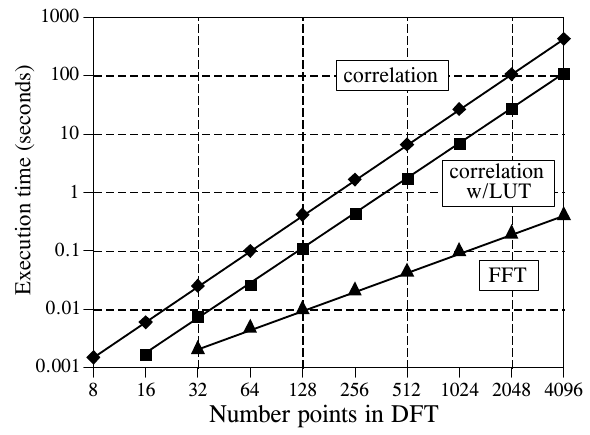
\includegraphics[width=0.492\linewidth,height=0.8\textheight,keepaspectratio]{assets/ch12/fig12-08.png}
\caption*{\textbf{图 12-8　计算 DFT 的执行时间。} 相关法指表 12-2
描述的算法。预先算好正弦和余弦值并存进查找表（LUT），可以让这种方法更快。当
DFT 长于 16 点时，FFT（表 12-3）是最快的算法。图中的时间是在 100 MHz
奔腾处理器上测得的。 （Execution time (seconds) = 执行时间（秒），Number
points in DFT = DFT 的点数；correlation = 相关法，correlation w/LUT =
使用查找表的相关法，FFT = FFT。）}
\end{figure}

FFT 除了速度快，还有另一个优点：因为计算次数少，舍入误差更小，所以 FFT
算得更精确。这可以这样演示：对一个任意信号做 FFT，再把得到的频谱送进逆
FFT。这就重建了原始时域信号，只是多了计算带来的舍入噪声。计算两个信号之差的标准差，就能得到刻画这种噪声的一个数。作为对比，可以用相关法计算的
DFT 及相应的逆 DFT 重复同样的过程。FFT 的舍入噪声与相关法 DFT
相比如何？请看图 12-9。

\begin{figure}[htbp]
\centering
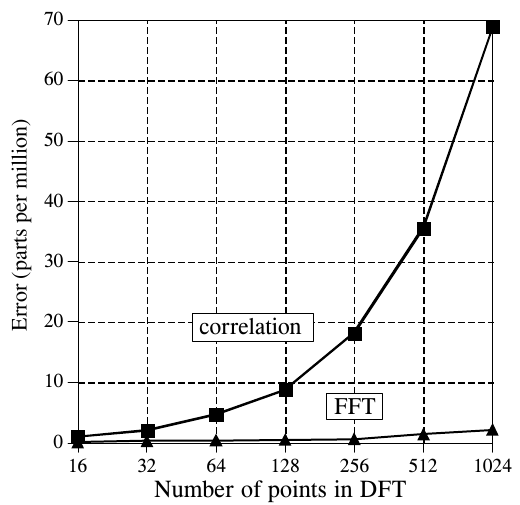
\includegraphics[width=0.433\linewidth,height=0.8\textheight,keepaspectratio]{assets/ch12/fig12-09.png}
\caption*{\textbf{图 12-9　DFT 的精度。} FFT 计算 DFT
比相关法快，同时舍入误差也更小。 （Error (parts per million) =
误差（百万分之一，ppm），Number of points in DFT = DFT
的点数；correlation = 相关法，FFT = FFT。）}
\end{figure}

\texttt{c/table12-5\_inverse\_fft.c}
按上文的方法重做了这个实验：全程单精度，随机信号正变换再逆变换，取原信号与还原信号之差的标准差。实测结果如下（ppm）：

\begingroup\scriptsize\setlength{\tabcolsep}{3pt}

{\def\LTcaptype{none} % do not increment counter
\begin{longtable}[]{@{}llllllll@{}}
\toprule\noalign{}
DFT 点数 & 16 & 32 & 64 & 128 & 256 & 512 & 1024 \\
\midrule\noalign{}
\endhead
\bottomrule\noalign{}
\endlastfoot
FFT & 0.04 & 0.10 & 0.12 & 0.22 & 0.25 & 0.72 & 0.92 \\
相关法 & 0.24 & 0.93 & 2.2 & 3.3 & 8.2 & 14 & 32 \\
\end{longtable}
}

\endgroup

趋势与图 12-9 一致：相关法的误差随 N 快速增长，FFT 一直维持在 1 ppm
左右。具体数值比书上小（书上 1024 点时约 69 ppm 和 2
ppm），这与随机信号的幅度和编译器、浮点库的实现有关。相关法误差大的一个主要原因是它要算
sin(2πki/N)，角度最大接近
2πN，单精度表示这么大的角度本身就有舍入误差；如果先用双精度算好正弦值再转成单精度，两种方法的误差就差不多了。

\section{进一步提速}

有几种技术能让 FFT 更快，不过提升只有 20～40\%
左右。其中一种方法是让时域分解提前两个阶段停下来，此时每个信号只有四个点。不再计算最后两个阶段，而是利用四点正弦、余弦波的简单性，用高度优化的代码直接跳到频域。

另一种流行的算法消除了因时域虚部为零、频谱对称而造成的无用计算。换句话说，把
FFT 修改成计算实数 DFT，而不是复数 DFT。这类算法叫实数 FFT(real FFT)
和实数逆 FFT(real Inverse FFT)（或类似的名字）。可以预期它们比常规 FFT
程序快 30\% 左右。表 12-6 和表 12-7 给出了这两种算法的程序。

\textbf{表 12-6　实数信号的逆 FFT。}（注释已译成中文）

\begin{Shaded}
\begin{Highlighting}[]
\NormalTok{4000 \textquotesingle{}INVERSE FFT FOR REAL SIGNALS}
\NormalTok{4010 \textquotesingle{}进入时，N\% 是 IDFT 的点数，REX[ ] 和}
\NormalTok{4020 \textquotesingle{}IMX[ ] 是频域的实部和虚部，下标从}
\NormalTok{4030 \textquotesingle{}0 到 N\%/2。REX[ ] 和 IMX[ ] 的其余采样被忽略。}
\NormalTok{4040 \textquotesingle{}返回时，REX[ ] 存放实时域信号，IMX[ ] 全为零。}
\NormalTok{4050 \textquotesingle{}}
\NormalTok{4060 \textquotesingle{}}
\NormalTok{4070 FOR K\% = (N\%/2+1) TO (N\%{-}1)                        \textquotesingle{}让频域对称}
\NormalTok{4080 REX[K\%] = REX[N\%{-}K\%]                               \textquotesingle{}（同表 12{-}1）}
\NormalTok{4090 IMX[K\%] = {-}IMX[N\%{-}K\%]}
\NormalTok{4100 NEXT K\%}
\NormalTok{4110 \textquotesingle{}}
\NormalTok{4120 FOR K\% = 0 TO N\%{-}1                                 \textquotesingle{}把实部和虚部相加}
\NormalTok{4130 REX[K\%] = REX[K\%]+IMX[K\%]}
\NormalTok{4140 NEXT K\%}
\NormalTok{4150 \textquotesingle{}}
\NormalTok{4160 GOSUB 3000                                         \textquotesingle{}计算正向实数 DFT（表 12{-}6）}
\NormalTok{4170 \textquotesingle{}}
\NormalTok{4180 FOR I\% = 0 TO N\%{-}1                                 \textquotesingle{}把实部和虚部相加，}
\NormalTok{4190 REX[I\%] = (REX[I\%]+IMX[I\%])/N\%                     \textquotesingle{}并把时域除以 N\%}
\NormalTok{4200 IMX[I\%] = 0}
\NormalTok{4210 NEXT I\%}
\NormalTok{4220 \textquotesingle{}}
\NormalTok{4230 RETURN}
\end{Highlighting}
\end{Shaded}

\begin{quote}
\textbf{译注：} 第 4160 行注释写''表 12-6''，即本表自己；实际调用的第
3000 行子程序是表 12-7 的实数
FFT。另外，``实部加虚部、做正变换、再实部加虚部''之所以能完成逆变换，用的是哈特利变换(Hartley
transform)的性质，原书没有解释。
\end{quote}

\textbf{C 实现}（完整可编译版本见
\texttt{c/table12-6\_real\_inverse\_fft.c}，文件里自带一份表 12-4 的 FFT
和表 12-7 的实数 FFT）：

\begin{Shaded}
\begin{Highlighting}[]
\CommentTok{/* 4000：实数逆 FFT */}
\DataTypeTok{static} \DataTypeTok{void}\NormalTok{ real\_inverse\_fft}\OperatorTok{(}\DataTypeTok{double} \OperatorTok{*}\NormalTok{rex}\OperatorTok{,} \DataTypeTok{double} \OperatorTok{*}\NormalTok{imx}\OperatorTok{,} \DataTypeTok{int}\NormalTok{ n}\OperatorTok{)}
\OperatorTok{\{}
    \ControlFlowTok{for} \OperatorTok{(}\DataTypeTok{int}\NormalTok{ k }\OperatorTok{=}\NormalTok{ n }\OperatorTok{/} \DecValTok{2} \OperatorTok{+} \DecValTok{1}\OperatorTok{;}\NormalTok{ k }\OperatorTok{\textless{}=}\NormalTok{ n }\OperatorTok{{-}} \DecValTok{1}\OperatorTok{;}\NormalTok{ k}\OperatorTok{++)} \OperatorTok{\{}  \CommentTok{/* 4070～4100：让频域对称（同表 12{-}1） */}
\NormalTok{        rex}\OperatorTok{[}\NormalTok{k}\OperatorTok{]} \OperatorTok{=}\NormalTok{ rex}\OperatorTok{[}\NormalTok{n }\OperatorTok{{-}}\NormalTok{ k}\OperatorTok{];}
\NormalTok{        imx}\OperatorTok{[}\NormalTok{k}\OperatorTok{]} \OperatorTok{=} \OperatorTok{{-}}\NormalTok{imx}\OperatorTok{[}\NormalTok{n }\OperatorTok{{-}}\NormalTok{ k}\OperatorTok{];}
    \OperatorTok{\}}

    \ControlFlowTok{for} \OperatorTok{(}\DataTypeTok{int}\NormalTok{ k }\OperatorTok{=} \DecValTok{0}\OperatorTok{;}\NormalTok{ k }\OperatorTok{\textless{}=}\NormalTok{ n }\OperatorTok{{-}} \DecValTok{1}\OperatorTok{;}\NormalTok{ k}\OperatorTok{++)}            \CommentTok{/* 4120～4140：实部和虚部相加 */}
\NormalTok{        rex}\OperatorTok{[}\NormalTok{k}\OperatorTok{]} \OperatorTok{=}\NormalTok{ rex}\OperatorTok{[}\NormalTok{k}\OperatorTok{]} \OperatorTok{+}\NormalTok{ imx}\OperatorTok{[}\NormalTok{k}\OperatorTok{];}

\NormalTok{    real\_fft}\OperatorTok{(}\NormalTok{rex}\OperatorTok{,}\NormalTok{ imx}\OperatorTok{,}\NormalTok{ n}\OperatorTok{);}                      \CommentTok{/* 4160：做正向实数 FFT（原书注释误写为表 12{-}6，实为表 12{-}7） */}

    \ControlFlowTok{for} \OperatorTok{(}\DataTypeTok{int}\NormalTok{ i }\OperatorTok{=} \DecValTok{0}\OperatorTok{;}\NormalTok{ i }\OperatorTok{\textless{}=}\NormalTok{ n }\OperatorTok{{-}} \DecValTok{1}\OperatorTok{;}\NormalTok{ i}\OperatorTok{++)} \OperatorTok{\{}          \CommentTok{/* 4180～4210：实部虚部相加，再除以 N */}
\NormalTok{        rex}\OperatorTok{[}\NormalTok{i}\OperatorTok{]} \OperatorTok{=} \OperatorTok{(}\NormalTok{rex}\OperatorTok{[}\NormalTok{i}\OperatorTok{]} \OperatorTok{+}\NormalTok{ imx}\OperatorTok{[}\NormalTok{i}\OperatorTok{])} \OperatorTok{/}\NormalTok{ n}\OperatorTok{;}
\NormalTok{        imx}\OperatorTok{[}\NormalTok{i}\OperatorTok{]} \OperatorTok{=} \DecValTok{0}\OperatorTok{;}
    \OperatorTok{\}}
\OperatorTok{\}}
\end{Highlighting}
\end{Shaded}

运行结果：随机实信号经实数 FFT 变到频域，只把第 0～N/2 点交给实数逆
FFT（其余点故意写成垃圾值 999），还原结果与原信号最大偏差 N=8 时
1.1e-16，N=64 时 5.3e-16，N=1024 时 1.8e-14。

使用实数 FFT
有两个小缺点。第一，代码长了大约一倍。你的计算机并不在乎，但你得花时间把别人的程序改到自己的机器上运行。第二，调试这些程序稍难一些，因为你不能再用对称性来检查它是否工作正常：这些算法强制时域虚部为零、频域左右对称。调试时，要检查它们的输出与常规
FFT 算法是否一致。

图 12-10 和图 12-11 说明了实数 FFT 的工作原理。在图 12-10 中，(a) 和 (b)
是一个时域信号：实部是一个脉冲，虚部全为零。(c) 和 (d)
是对应的频谱。如前所述，频域的实部关于第 0 个和第 N/2 个采样偶对称(even
symmetry)，虚部关于同样这两点奇对称(odd symmetry)。

\begin{figure}[htbp]
\centering
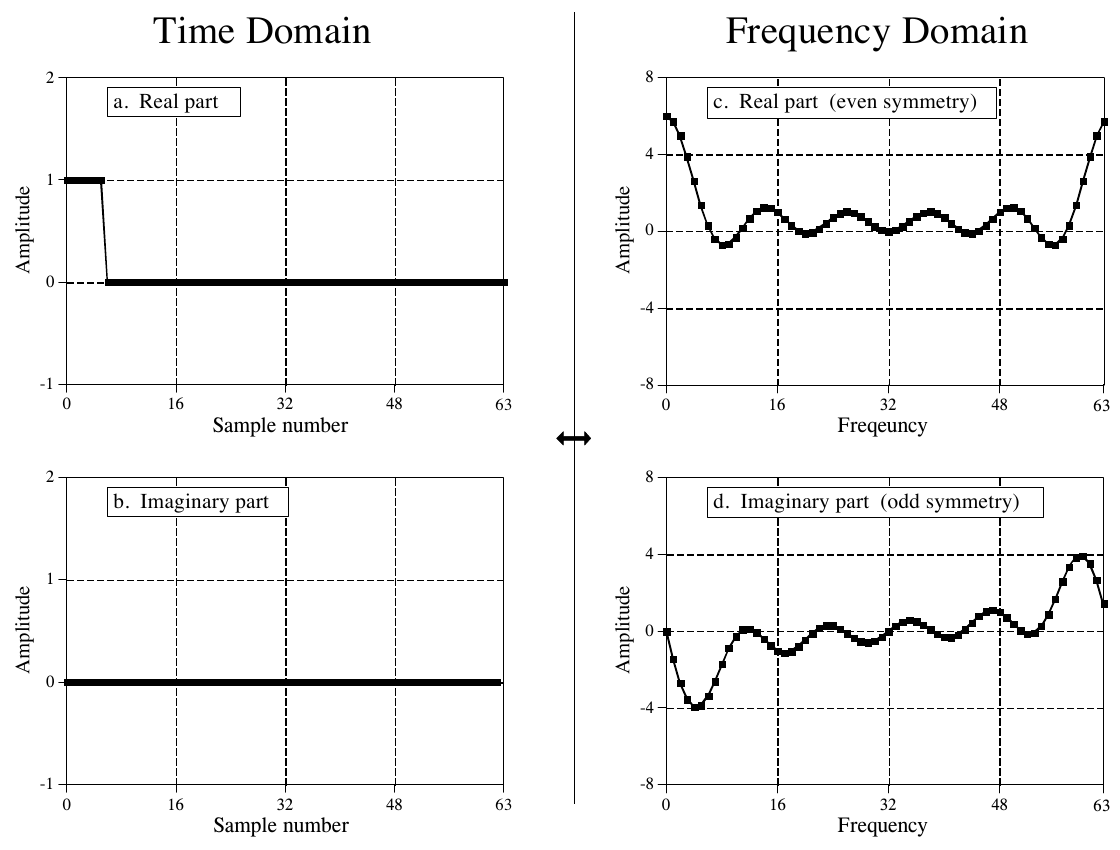
\includegraphics[width=0.933\linewidth,height=0.8\textheight,keepaspectratio]{assets/ch12/fig12-10.png}
\caption*{\textbf{图 12-10　DFT 的实部对称性。} （Time Domain = 时域，Frequency
Domain = 频域；a. Real part = 实部，b. Imaginary part = 虚部，c.~Real
part (even symmetry) = 实部（偶对称），d.~Imaginary part (odd symmetry)
= 虚部（奇对称）。Amplitude = 幅度，Sample number = 采样序号，Frequency
= 频率（(c) 的横轴标注原书误拼为 Freqeuncy）。）}
\end{figure}

再看图
12-11，这时脉冲在时域的虚部，实部全为零。频域的对称性反了过来：实部是奇对称，虚部是偶对称。这种情况将在第
29 章讨论（译注：实为第 31 章）。眼下就先接受复数 DFT 是这样表现的。

\begin{figure}[htbp]
\centering
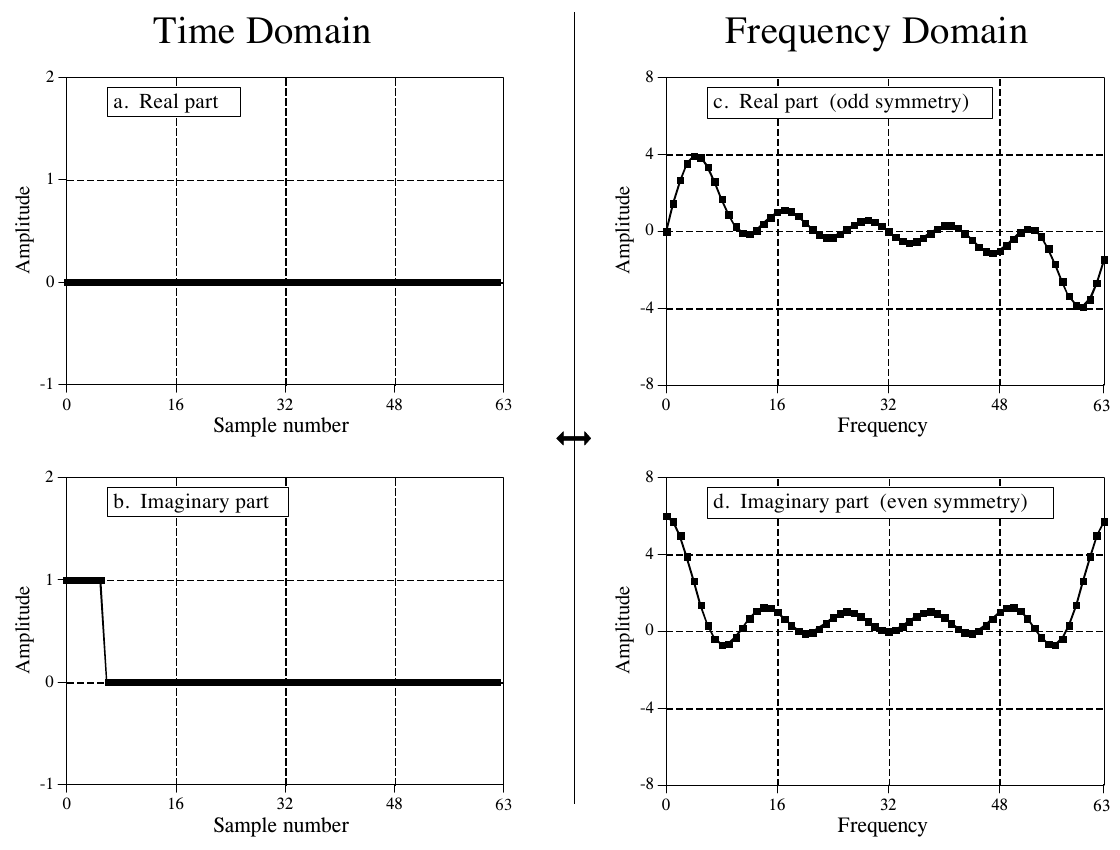
\includegraphics[width=0.933\linewidth,height=0.8\textheight,keepaspectratio]{assets/ch12/fig12-11.png}
\caption*{\textbf{图 12-11　DFT 的虚部对称性。} （a. Real part = 实部，b.
Imaginary part = 虚部，c.~Real part (odd symmetry) =
实部（奇对称），d.~Imaginary part (even symmetry) =
虚部（偶对称）。其余标注同图 12-10。）}
\end{figure}

如果时域的两部分都有信号呢？根据可加性，频域就是两个频谱之和。关键在于：由这两种对称性组成的频谱，可以完美地分离成两个分量信号。这可以用偶/奇分解(even/odd
decomposition)来实现，该方法在第 6 章讨论过（译注：实为第 5
章）。换句话说，花一次 FFT 的代价就能算出两个实数
DFT。把一个信号放进时域实部，另一个信号放进时域虚部。计算复数
DFT（当然是用
FFT）之后，再用偶/奇分解把两个频谱分开。当需要让两个或更多信号通过 FFT
时，这种技术能把执行时间减少约
40\%。之所以达不到整整两倍，是因为偶/奇分解本身也要花计算时间。这是一种相对简单、陷阱很少的技术，完全不像从零写一个
FFT 程序那样难。

下一步是修改算法，让单个 DFT
算得更快。方法很难看，但做法如下。用交错分解把输入信号一分为二：N/2
个偶数点放进时域信号的实部，N/2 个奇数点放进虚部。然后计算一个 N/2 点
FFT，所需时间大约是 N 点 FFT
的一半。再用偶/奇分解把得到的频域分开，得到两个交错时域信号的频谱。最后，像
FFT 的最后一个合成阶段那样，把这两个频谱合并成一个频谱。

作为本章的结尾，不妨这样看：FFT
之于数字信号处理，就像晶体管之于电子学。它是这门技术的基石；这一领域里人人都知道它的特性和用法，但真正懂得其内部工作细节的，只有少数专家。

\textbf{表 12-7　实数信号的 FFT。}（注释已译成中文）

\begin{Shaded}
\begin{Highlighting}[]
\NormalTok{3000 \textquotesingle{}FFT FOR REAL SIGNALS}
\NormalTok{3010 \textquotesingle{}进入时，N\% 是 DFT 的点数，REX[ ] 存放}
\NormalTok{3020 \textquotesingle{}实输入信号，IMX[ ] 中的值被忽略。返回时，}
\NormalTok{3030 \textquotesingle{}REX[ ] 和 IMX[ ] 存放 DFT 的输出。所有信号都从 0 到 N\%{-}1。}
\NormalTok{3040 \textquotesingle{}}
\NormalTok{3050 NH\% = N\%/2{-}1                                   \textquotesingle{}把偶数点和奇数点分开}
\NormalTok{3060 FOR I\% = 0 TO NH\%}
\NormalTok{3070 REX(I\%) = REX(2*I\%)}
\NormalTok{3080 IMX(I\%) = REX(2*I\%+1)}
\NormalTok{3090 NEXT I\%}
\NormalTok{3100 \textquotesingle{}}
\NormalTok{3110 N\% = N\%/2                                      \textquotesingle{}计算 N\%/2 点 FFT}
\NormalTok{3120 GOSUB 1000                                     \textquotesingle{}（GOSUB 1000 是表 12{-}3 的 FFT）}
\NormalTok{3130 N\% = N\%*2}
\NormalTok{3140 \textquotesingle{}}
\NormalTok{3150 NM1\% = N\%{-}1                                    \textquotesingle{}频域的偶/奇分解}
\NormalTok{3160 ND2\% = N\%/2}
\NormalTok{3170 N4\% = N\%/4{-}1}
\NormalTok{3180 FOR I\% = 1 TO N4\%}
\NormalTok{3190 IM\% = ND2\%{-}I\%}
\NormalTok{3200 IP2\% = I\%+ND2\%}
\NormalTok{3210 IPM\% = IM\%+ND2\%}
\NormalTok{3220 REX(IP2\%) = (IMX(I\%) + IMX(IM\%))/2}
\NormalTok{3230 REX(IPM\%) = REX(IP2\%)}
\NormalTok{3240 IMX(IP2\%) = {-}(REX(I\%) {-} REX(IM\%))/2}
\NormalTok{3250 IMX(IPM\%) = {-}IMX(IP2\%)}
\NormalTok{3260 REX(I\%) = (REX(I\%) + REX(IM\%))/2}
\NormalTok{3270 REX(IM\%) = REX(I\%)}
\NormalTok{3280 IMX(I\%) = (IMX(I\%) {-} IMX(IM\%))/2}
\NormalTok{3290 IMX(IM\%) = {-}IMX(I\%)}
\NormalTok{3300 NEXT I\%}
\NormalTok{3310 REX(N\%*3/4) = IMX(N\%/4)}
\NormalTok{3320 REX(ND2\%) = IMX(0)}
\NormalTok{3330 IMX(N\%*3/4) = 0}
\NormalTok{3340 IMX(ND2\%) = 0}
\NormalTok{3350 IMX(N\%/4) = 0}
\NormalTok{3360 IMX(0) = 0}
\NormalTok{3370 \textquotesingle{}}
\NormalTok{3380 PI = 3.14159265                                          \textquotesingle{}补做 FFT 的最后一级}
\NormalTok{3390 L\% = CINT(LOG(N\%)/LOG(2))}
\NormalTok{3400 LE\% = CINT(2\^{}L\%)}
\NormalTok{3410 LE2\% = LE\%/2}
\NormalTok{3420 UR = 1}
\NormalTok{3430 UI = 0}
\NormalTok{3440 SR = COS(PI/LE2\%)}
\NormalTok{3450 SI = {-}SIN(PI/LE2\%)}
\NormalTok{3460 FOR J\% = 1 TO LE2\%}
\NormalTok{3470 JM1\% = J\%{-}1}
\NormalTok{3480 FOR I\% = JM1\% TO NM1\% STEP LE\%}
\NormalTok{3490 IP\% = I\%+LE2\%}
\NormalTok{3500 TR = REX[IP\%]*UR {-} IMX[IP\%]*UI}
\NormalTok{3510 TI = REX[IP\%]*UI + IMX[IP\%]*UR}
\NormalTok{3520 REX[IP\%] = REX[I\%]{-}TR}
\NormalTok{3530 IMX[IP\%] = IMX[I\%]{-}TI}
\NormalTok{3540 REX[I\%] = REX[I\%]+TR}
\NormalTok{3550 IMX[I\%] = IMX[I\%]+TI}
\NormalTok{3560 NEXT I\%}
\NormalTok{3570 TR = UR}
\NormalTok{3580 UR = TR*SR {-} UI*SI}
\NormalTok{3590 UI = TR*SI + UI*SR}
\NormalTok{3600 NEXT J\%}
\NormalTok{3610 RETURN}
\end{Highlighting}
\end{Shaded}

\begin{quote}
\textbf{译注：} 第 3120 行注释写''表 12-3''，实际调用的是表 12-4 的
BASIC 版 FFT。原程序中数组括号 ( ) 和 {[} {]} 混用，含义相同。
\end{quote}

\textbf{C 实现}（完整可编译版本见
\texttt{c/table12-7\_real\_fft.c}，文件里自带一份表 12-4 的 FFT）：

\begin{Shaded}
\begin{Highlighting}[]
\CommentTok{/* 3000：实数 FFT。进入时 rex[] 是实信号（imx[] 内容忽略），返回时 rex/imx 是 0～n{-}1 的完整频谱 */}
\DataTypeTok{static} \DataTypeTok{void}\NormalTok{ real\_fft}\OperatorTok{(}\DataTypeTok{double} \OperatorTok{*}\NormalTok{rex}\OperatorTok{,} \DataTypeTok{double} \OperatorTok{*}\NormalTok{imx}\OperatorTok{,} \DataTypeTok{int}\NormalTok{ n}\OperatorTok{)}
\OperatorTok{\{}
    \DataTypeTok{int}\NormalTok{ nh }\OperatorTok{=}\NormalTok{ n }\OperatorTok{/} \DecValTok{2} \OperatorTok{{-}} \DecValTok{1}\OperatorTok{;}                         \CommentTok{/* 3050：拆开偶数点和奇数点 */}
    \ControlFlowTok{for} \OperatorTok{(}\DataTypeTok{int}\NormalTok{ i }\OperatorTok{=} \DecValTok{0}\OperatorTok{;}\NormalTok{ i }\OperatorTok{\textless{}=}\NormalTok{ nh}\OperatorTok{;}\NormalTok{ i}\OperatorTok{++)} \OperatorTok{\{}             \CommentTok{/* 3060～3090：偶数点进实部，奇数点进虚部 */}
\NormalTok{        rex}\OperatorTok{[}\NormalTok{i}\OperatorTok{]} \OperatorTok{=}\NormalTok{ rex}\OperatorTok{[}\DecValTok{2} \OperatorTok{*}\NormalTok{ i}\OperatorTok{];}                    \CommentTok{/* 从小下标往上写，不会覆盖还没读的点 */}
\NormalTok{        imx}\OperatorTok{[}\NormalTok{i}\OperatorTok{]} \OperatorTok{=}\NormalTok{ rex}\OperatorTok{[}\DecValTok{2} \OperatorTok{*}\NormalTok{ i }\OperatorTok{+} \DecValTok{1}\OperatorTok{];}
    \OperatorTok{\}}

\NormalTok{    fft}\OperatorTok{(}\NormalTok{rex}\OperatorTok{,}\NormalTok{ imx}\OperatorTok{,}\NormalTok{ n }\OperatorTok{/} \DecValTok{2}\OperatorTok{);}                       \CommentTok{/* 3110～3130：做 N/2 点 FFT */}

    \DataTypeTok{int}\NormalTok{ nm1 }\OperatorTok{=}\NormalTok{ n }\OperatorTok{{-}} \DecValTok{1}\OperatorTok{,}\NormalTok{ nd2 }\OperatorTok{=}\NormalTok{ n }\OperatorTok{/} \DecValTok{2}\OperatorTok{,}\NormalTok{ n4 }\OperatorTok{=}\NormalTok{ n }\OperatorTok{/} \DecValTok{4} \OperatorTok{{-}} \DecValTok{1}\OperatorTok{;}   \CommentTok{/* 3150～3170：频域的偶/奇分解 */}
    \ControlFlowTok{for} \OperatorTok{(}\DataTypeTok{int}\NormalTok{ i }\OperatorTok{=} \DecValTok{1}\OperatorTok{;}\NormalTok{ i }\OperatorTok{\textless{}=}\NormalTok{ n4}\OperatorTok{;}\NormalTok{ i}\OperatorTok{++)} \OperatorTok{\{}             \CommentTok{/* 3180：每次处理一对对称点 I 和 N/2{-}I */}
        \DataTypeTok{int}\NormalTok{ im }\OperatorTok{=}\NormalTok{ nd2 }\OperatorTok{{-}}\NormalTok{ i}\OperatorTok{;}                       \CommentTok{/* 3190 */}
        \DataTypeTok{int}\NormalTok{ ip2 }\OperatorTok{=}\NormalTok{ i }\OperatorTok{+}\NormalTok{ nd2}\OperatorTok{;}                      \CommentTok{/* 3200 */}
        \DataTypeTok{int}\NormalTok{ ipm }\OperatorTok{=}\NormalTok{ im }\OperatorTok{+}\NormalTok{ nd2}\OperatorTok{;}                     \CommentTok{/* 3210 */}
\NormalTok{        rex}\OperatorTok{[}\NormalTok{ip2}\OperatorTok{]} \OperatorTok{=} \OperatorTok{(}\NormalTok{imx}\OperatorTok{[}\NormalTok{i}\OperatorTok{]} \OperatorTok{+}\NormalTok{ imx}\OperatorTok{[}\NormalTok{im}\OperatorTok{])} \OperatorTok{/} \DecValTok{2}\OperatorTok{;}      \CommentTok{/* 3220～3250：奇数点信号的频谱，放在后半段 */}
\NormalTok{        rex}\OperatorTok{[}\NormalTok{ipm}\OperatorTok{]} \OperatorTok{=}\NormalTok{ rex}\OperatorTok{[}\NormalTok{ip2}\OperatorTok{];}
\NormalTok{        imx}\OperatorTok{[}\NormalTok{ip2}\OperatorTok{]} \OperatorTok{=} \OperatorTok{{-}(}\NormalTok{rex}\OperatorTok{[}\NormalTok{i}\OperatorTok{]} \OperatorTok{{-}}\NormalTok{ rex}\OperatorTok{[}\NormalTok{im}\OperatorTok{])} \OperatorTok{/} \DecValTok{2}\OperatorTok{;}
\NormalTok{        imx}\OperatorTok{[}\NormalTok{ipm}\OperatorTok{]} \OperatorTok{=} \OperatorTok{{-}}\NormalTok{imx}\OperatorTok{[}\NormalTok{ip2}\OperatorTok{];}
\NormalTok{        rex}\OperatorTok{[}\NormalTok{i}\OperatorTok{]} \OperatorTok{=} \OperatorTok{(}\NormalTok{rex}\OperatorTok{[}\NormalTok{i}\OperatorTok{]} \OperatorTok{+}\NormalTok{ rex}\OperatorTok{[}\NormalTok{im}\OperatorTok{])} \OperatorTok{/} \DecValTok{2}\OperatorTok{;}        \CommentTok{/* 3260～3290：偶数点信号的频谱，留在前半段 */}
\NormalTok{        rex}\OperatorTok{[}\NormalTok{im}\OperatorTok{]} \OperatorTok{=}\NormalTok{ rex}\OperatorTok{[}\NormalTok{i}\OperatorTok{];}
\NormalTok{        imx}\OperatorTok{[}\NormalTok{i}\OperatorTok{]} \OperatorTok{=} \OperatorTok{(}\NormalTok{imx}\OperatorTok{[}\NormalTok{i}\OperatorTok{]} \OperatorTok{{-}}\NormalTok{ imx}\OperatorTok{[}\NormalTok{im}\OperatorTok{])} \OperatorTok{/} \DecValTok{2}\OperatorTok{;}
\NormalTok{        imx}\OperatorTok{[}\NormalTok{im}\OperatorTok{]} \OperatorTok{=} \OperatorTok{{-}}\NormalTok{imx}\OperatorTok{[}\NormalTok{i}\OperatorTok{];}
    \OperatorTok{\}}
\NormalTok{    rex}\OperatorTok{[}\NormalTok{n }\OperatorTok{*} \DecValTok{3} \OperatorTok{/} \DecValTok{4}\OperatorTok{]} \OperatorTok{=}\NormalTok{ imx}\OperatorTok{[}\NormalTok{n }\OperatorTok{/} \DecValTok{4}\OperatorTok{];}                \CommentTok{/* 3310～3360：自身对称的 0 和 N/4 两点单独处理 */}
\NormalTok{    rex}\OperatorTok{[}\NormalTok{nd2}\OperatorTok{]} \OperatorTok{=}\NormalTok{ imx}\OperatorTok{[}\DecValTok{0}\OperatorTok{];}
\NormalTok{    imx}\OperatorTok{[}\NormalTok{n }\OperatorTok{*} \DecValTok{3} \OperatorTok{/} \DecValTok{4}\OperatorTok{]} \OperatorTok{=} \DecValTok{0}\OperatorTok{;}
\NormalTok{    imx}\OperatorTok{[}\NormalTok{nd2}\OperatorTok{]} \OperatorTok{=} \DecValTok{0}\OperatorTok{;}
\NormalTok{    imx}\OperatorTok{[}\NormalTok{n }\OperatorTok{/} \DecValTok{4}\OperatorTok{]} \OperatorTok{=} \DecValTok{0}\OperatorTok{;}
\NormalTok{    imx}\OperatorTok{[}\DecValTok{0}\OperatorTok{]} \OperatorTok{=} \DecValTok{0}\OperatorTok{;}

    \DataTypeTok{int}\NormalTok{ l }\OperatorTok{=} \OperatorTok{(}\DataTypeTok{int}\OperatorTok{)}\NormalTok{lround}\OperatorTok{(}\NormalTok{log}\OperatorTok{(}\NormalTok{n}\OperatorTok{)} \OperatorTok{/}\NormalTok{ log}\OperatorTok{(}\DecValTok{2}\OperatorTok{));}       \CommentTok{/* 3380～3600：补做 FFT 的最后一级 */}
    \DataTypeTok{int}\NormalTok{ le }\OperatorTok{=} \DecValTok{1} \OperatorTok{\textless{}\textless{}}\NormalTok{ l}\OperatorTok{;}                            \CommentTok{/* 3400：最后一级 LE = N */}
    \DataTypeTok{int}\NormalTok{ le2 }\OperatorTok{=}\NormalTok{ le }\OperatorTok{/} \DecValTok{2}\OperatorTok{;}
    \DataTypeTok{double}\NormalTok{ ur }\OperatorTok{=} \FloatTok{1.0}\OperatorTok{,}\NormalTok{ ui }\OperatorTok{=} \FloatTok{0.0}\OperatorTok{,}\NormalTok{ sr }\OperatorTok{=}\NormalTok{ cos}\OperatorTok{(}\NormalTok{PI }\OperatorTok{/}\NormalTok{ le2}\OperatorTok{),}\NormalTok{ si }\OperatorTok{=} \OperatorTok{{-}}\NormalTok{sin}\OperatorTok{(}\NormalTok{PI }\OperatorTok{/}\NormalTok{ le2}\OperatorTok{);}
    \ControlFlowTok{for} \OperatorTok{(}\DataTypeTok{int}\NormalTok{ j }\OperatorTok{=} \DecValTok{1}\OperatorTok{;}\NormalTok{ j }\OperatorTok{\textless{}=}\NormalTok{ le2}\OperatorTok{;}\NormalTok{ j}\OperatorTok{++)} \OperatorTok{\{}            \CommentTok{/* 3460 */}
        \DataTypeTok{int}\NormalTok{ jm1 }\OperatorTok{=}\NormalTok{ j }\OperatorTok{{-}} \DecValTok{1}\OperatorTok{;}
        \ControlFlowTok{for} \OperatorTok{(}\DataTypeTok{int}\NormalTok{ i }\OperatorTok{=}\NormalTok{ jm1}\OperatorTok{;}\NormalTok{ i }\OperatorTok{\textless{}=}\NormalTok{ nm1}\OperatorTok{;}\NormalTok{ i }\OperatorTok{+=}\NormalTok{ le}\OperatorTok{)} \OperatorTok{\{}  \CommentTok{/* 3480：最后一级每个 J 只有一个蝶形 */}
            \DataTypeTok{int}\NormalTok{ ip }\OperatorTok{=}\NormalTok{ i }\OperatorTok{+}\NormalTok{ le2}\OperatorTok{;}
            \DataTypeTok{double}\NormalTok{ tr }\OperatorTok{=}\NormalTok{ rex}\OperatorTok{[}\NormalTok{ip}\OperatorTok{]} \OperatorTok{*}\NormalTok{ ur }\OperatorTok{{-}}\NormalTok{ imx}\OperatorTok{[}\NormalTok{ip}\OperatorTok{]} \OperatorTok{*}\NormalTok{ ui}\OperatorTok{;}    \CommentTok{/* 3500～3550：蝶形运算 */}
            \DataTypeTok{double}\NormalTok{ ti }\OperatorTok{=}\NormalTok{ rex}\OperatorTok{[}\NormalTok{ip}\OperatorTok{]} \OperatorTok{*}\NormalTok{ ui }\OperatorTok{+}\NormalTok{ imx}\OperatorTok{[}\NormalTok{ip}\OperatorTok{]} \OperatorTok{*}\NormalTok{ ur}\OperatorTok{;}
\NormalTok{            rex}\OperatorTok{[}\NormalTok{ip}\OperatorTok{]} \OperatorTok{=}\NormalTok{ rex}\OperatorTok{[}\NormalTok{i}\OperatorTok{]} \OperatorTok{{-}}\NormalTok{ tr}\OperatorTok{;}
\NormalTok{            imx}\OperatorTok{[}\NormalTok{ip}\OperatorTok{]} \OperatorTok{=}\NormalTok{ imx}\OperatorTok{[}\NormalTok{i}\OperatorTok{]} \OperatorTok{{-}}\NormalTok{ ti}\OperatorTok{;}
\NormalTok{            rex}\OperatorTok{[}\NormalTok{i}\OperatorTok{]} \OperatorTok{=}\NormalTok{ rex}\OperatorTok{[}\NormalTok{i}\OperatorTok{]} \OperatorTok{+}\NormalTok{ tr}\OperatorTok{;}
\NormalTok{            imx}\OperatorTok{[}\NormalTok{i}\OperatorTok{]} \OperatorTok{=}\NormalTok{ imx}\OperatorTok{[}\NormalTok{i}\OperatorTok{]} \OperatorTok{+}\NormalTok{ ti}\OperatorTok{;}
        \OperatorTok{\}}
        \DataTypeTok{double}\NormalTok{ tr }\OperatorTok{=}\NormalTok{ ur}\OperatorTok{;}                         \CommentTok{/* 3570～3590 */}
\NormalTok{        ur }\OperatorTok{=}\NormalTok{ tr }\OperatorTok{*}\NormalTok{ sr }\OperatorTok{{-}}\NormalTok{ ui }\OperatorTok{*}\NormalTok{ si}\OperatorTok{;}
\NormalTok{        ui }\OperatorTok{=}\NormalTok{ tr }\OperatorTok{*}\NormalTok{ si }\OperatorTok{+}\NormalTok{ ui }\OperatorTok{*}\NormalTok{ sr}\OperatorTok{;}
    \OperatorTok{\}}
\OperatorTok{\}}
\end{Highlighting}
\end{Shaded}

运行结果： - 随机实信号用实数 FFT 计算，与普通复数 FFT（虚部填
0）逐点比较，最大偏差 N=8 时 1.1e-16，N=64 时 1.8e-15，N=1024 时
1.2e-13。进入时故意在 IMX{[} {]} 里填了垃圾值，确认它确实被忽略。 - 1024
点各算 20000 次：复数 FFT 154 ms，实数 FFT 80
ms。这台机器上快了约一倍，比书上说的 30\% 还多。

% !TEX root = ../main.tex
% 本文件由 build-tex.sh 从 13-DSP指南-第13章中译.md 生成，改内容请改 md 后重新生成

\chapter{连续信号处理}\label{ch-13}

连续信号处理(continuous signal processing)是与 DSP
平行的一个领域，大多数技术几乎完全相同。例如，DSP
和连续信号处理都建立在线性、分解、卷积和傅里叶分析之上。由于连续信号无法直接在数字计算机中表示，本章不会有计算机程序。连续信号处理以数学为基础：信号用方程表示，系统把一个方程变成另一个方程。正如数字计算机是
DSP
的主要工具，微积分是连续信号处理的主要工具。这些技术已经用了几百年，远在计算机出现之前。

\section{冲激函数}

和离散信号一样，连续信号也可以分解成一组经过缩放和平移的冲激函数(delta
function)。区别在于，连续冲激函数比离散的冲激函数复杂得多，也抽象得多。我们不去定义连续冲激函数''是什么''，而是用它具有的特性来定义它。

用一个思想实验来说明。设想一个由线性元件（比如电阻、电容和电感）组成的电子电路。输入端接一台信号发生器，能产生各种形状的短脉冲。电路的输出接示波器，显示电路对每个输入脉冲产生的波形。我们想回答的问题是：输出脉冲的形状和输入脉冲的特性有什么关系？为了简化研究，我们只用比输出短得多的输入脉冲。例如，如果系统的响应以毫秒计，我们可能只用几微秒长的输入脉冲。

做了大量测量之后，我们得出三个结论。第一，输入脉冲的形状不影响输出信号的形状。图
13-1
说明了这一点：各种形状的短输入脉冲产生的输出脉冲形状完全一样。第二，输出波形的形状完全由系统的特性决定，即电阻、电容和电感的取值和连接方式。第三，输出脉冲的幅度与输入脉冲的面积成正比。例如，输入为''1
伏持续 1 微秒''\,``10 伏持续 0.1 微秒''``1000 伏持续 1
纳秒''等时，输出的幅度都相同。这个关系也允许输入脉冲的面积为负。例如，设想一个
2 伏、持续 2 微秒的脉冲，紧接着一个 −1 伏、持续 4
微秒的脉冲。输入信号的总面积为零，于是输出什么也不做。

足够短、具备这三个性质的输入信号叫冲激(impulse)。换句话说，冲激就是除一个形状任意的短促尖峰外全为零的信号。例如，对微波发射机来说，冲激可能要短到皮秒量级，因为它的电子器件以纳秒为单位响应。相比之下，一次持续好几年的火山喷发，对需要上千年才发生的地质变化来说，完全可以算一个冲激。

数学家不喜欢被某个具体系统束缚，常用''冲激''一词指一个短到对任何可能的系统都算冲激的信号，也就是无穷窄的信号。连续冲激函数就是这种冲激的归一化版本。具体地说，连续冲激函数在数学上由三条理想化的特性定义：(1)
信号必须无穷短；(2) 脉冲必须出现在时间零点；(3) 脉冲的面积必须为一。

既然冲激函数被定义为无穷窄、面积固定，那么它的幅度就隐含为无穷大。别为此烦恼，这完全无关紧要。幅度是冲激''形状''的一部分，你永远不会遇到幅度起作用的问题，不管它是不是无穷大。冲激函数是一个数学构造，不是真实世界的信号。真实世界中充当冲激函数的信号，总是有有限的持续时间和幅度。

和离散情形一样，连续冲激函数用数学符号 δ( )
表示。同样，连续系统对冲激函数的输出叫冲激响应(impulse response)，常记作
h( )。注意，连续信号用圆括号 ( ) 表示，而离散信号用方括号 {[}
{]}。本书和 DSP
的其他文献都用这种记法，但它并不通用。在图中，冲激画成竖直的箭头（见图
13-1d），箭头的长度表示冲激的面积。

为了更好地理解真实世界中的冲激，在夜里看看天空中的一颗行星和一颗恒星，比如火星和天狼星。用肉眼看，两者的亮度和大小差不多。这种相似的原因并不明显，因为观看的几何条件相差悬殊。火星直径约
6000 千米，离地球约 6000 万千米。相比之下，天狼星大约大 300
倍，远一百多万倍。按这些尺寸，火星看起来应该比天狼星大三千多倍。它们怎么会看起来一样呢？

\begin{figure}[htbp]
\centering
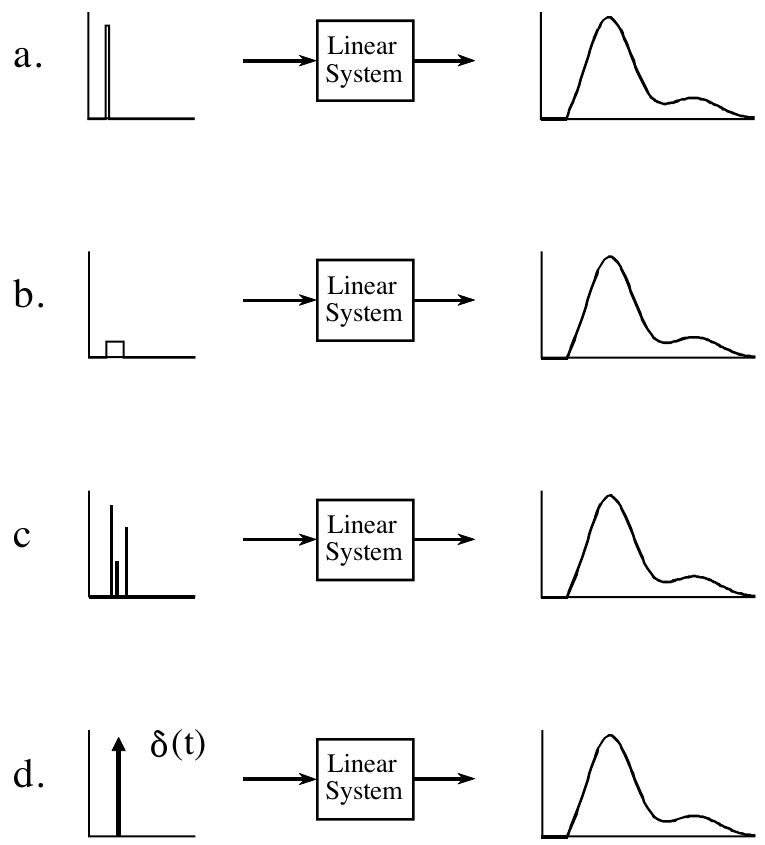
\includegraphics[width=0.637\linewidth,height=0.8\textheight,keepaspectratio]{assets/ch13/fig13-01.png}
\caption*{\textbf{图 13-1　连续冲激函数。}
如果线性系统的输入相对于它产生的输出很短，输出的形状就只取决于系统的特性，而与输入的形状无关。这样短的输入信号叫冲激。a、b、c
是对这个特定系统而言属于冲激的几种输入信号示例。冲激函数一词用来描述归一化的冲激，即出现在
t = 0、面积为一的冲激。(d) 给出了冲激函数的数学符号：一个竖直箭头和
δ(t)。 （Linear System = 线性系统。原书图注里 ``Figures a,b \& c'' 的 c
在图中缺了句点，无关紧要。）}
\end{figure}

它们看起来一样，是因为它们都小到对人类视觉系统来说算是冲激。我们感知到的形状是眼睛的冲激响应，而不是恒星或行星的真实图像。用一架小望远镜观察时这一点就很明显了：火星显出一个暗淡的圆盘，而天狼星仍然是一个明亮的冲激。这也是恒星会闪烁而行星不会的原因。恒星的像小到可以被大气中的颗粒或湍流短暂遮挡，而行星较大的像受到的影响要小得多。

\section{卷积}

和离散信号一样，连续信号的卷积(convolution)既可以从输入信号的角度看，也可以从输出信号的角度看。输入端视角最适合在概念上描述卷积怎样运作；输出端视角则描述了必须使用的数学。这些描述与第
6 章中离散信号的描述几乎完全一样。

图 13-2 展示了从输入端看卷积。输入信号 x(t) 通过一个以冲激响应 h(t)
刻画的系统，产生输出信号
y(t)。这可以写成熟悉的数学式：\(y(t) = x(t) * h(t)\)。输入信号被分成许多窄条，每一条都短到对系统来说算一个冲激。换句话说，输入信号被分解成无穷多个经过缩放和平移的冲激函数。每个冲激在输出信号中产生一个经过缩放和平移的冲激响应。最终的输出信号等于它们的综合效果，即所有单个响应之和。

\begin{figure}[htbp]
\centering
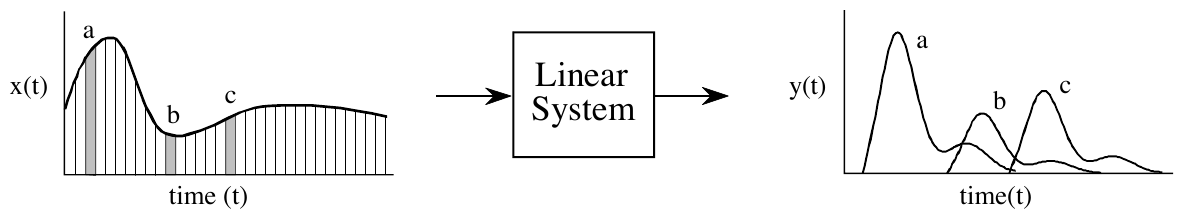
\includegraphics[width=0.988\linewidth,height=0.8\textheight,keepaspectratio]{assets/ch13/fig13-02.png}
\caption*{\textbf{图 13-2　从输入端看卷积。} 输入信号 x(t)
被分成许多窄段，每一段对系统来说都是一个冲激。输出信号 y(t)
是由此产生的、经过缩放和平移的各冲激响应之和。本图展示了输入信号中的三个点（a、b、c）怎样对输出信号作出贡献。
（Linear System = 线性系统，time (t) = 时间 (t)。）}
\end{figure}

要让这个方案行得通，窄条的宽度必须远小于系统响应的长度。当然，数学家会把它推到极致，让输入段无穷窄，把问题变成一个微积分问题。这样，输入端视角描述的就是输入信号中的一个点（或一个窄区域）怎样影响输出信号中较大的一段。

相比之下，输出端视角考察的是输出信号中的一个点怎样由输入信号的各个值决定。和离散信号一样，输出信号中的每个瞬时值都受输入信号中一段区间的影响，权重由左右翻转后的冲激响应给出。离散情形下，信号相乘后求和；连续情形下，信号相乘后积分。写成公式：

\textbf{公式 13-1}　卷积积分。这个公式定义了 \(y(t) = x(t) * h(t)\)
的含义。

\[y(t) = \int_{-\infty}^{+\infty} x(\tau)\, h(t-\tau)\, d\tau\]

这个公式叫卷积积分(convolution integral)，它是离散信号所用的卷积和（公式
6-1）的孪生兄弟。图 13-3
说明了怎样理解这个公式。目标是找到一个表达式，能算出输出信号在任意时刻 t
的值。第一步是更换用来遍历输入信号和冲激响应的自变量，即把 t 换成
τ（希腊字母 tau 的小写）。这样 x(t) 和 h(t) 分别变成 x(τ) 和
h(τ)。之所以要换变量名，是因为 t
已经用来表示正在计算的输出信号中的那个点了。下一步是把冲激响应左右翻转，变成
h(−τ)。再把翻转后的冲激响应平移到位置 t，表达式就变成
h(t−τ)。然后把输入信号与翻转并平移后的冲激响应相乘，对输入信号加权，即
x(τ)
h(t−τ)。最后，把这个加权后的输入信号从负无穷到正无穷积分，就得到输出信号的值，正如公式
13-1 所描述的。

如果你理解起来有困难，回头复习一下第 6 章中离散信号的同样概念。图 13-3
只不过是描述图 6-8
卷积机的另一种方式。唯一的区别是用积分代替了求和。把它当作你已知内容的扩展，而不是什么新东西。

\begin{figure}[htbp]
\centering
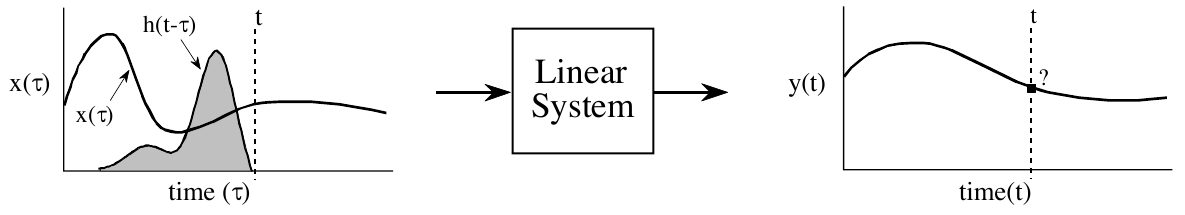
\includegraphics[width=0.988\linewidth,height=0.8\textheight,keepaspectratio]{assets/ch13/fig13-03.png}
\caption*{\textbf{图 13-3　从输出端看卷积。}
输出信号中的每个值都受输入信号中许多点的影响。本图中正在计算的是输出信号在时刻
t 的值。输入信号 x(τ) 被翻转并平移后的冲激响应 h(t−τ)
加权（相乘）。对加权后的输入信号积分，就得到输出点 y(t) 的值。 （Linear
System = 线性系统，time (τ) = 时间 (τ)；y(t) 图上的 ``?''
表示正在求的输出值。）}
\end{figure}

一个例子能说明连续卷积在实际问题中怎样使用、需要什么样的数学。图 13-4
是一个简单的连续线性系统：由一个电阻和一个电容组成的电子低通滤波器。如图所示，一个冲激进入这个系统后，输出会迅速跳到某个值，然后按指数衰减趋于零。换句话说，这个简单电子电路的冲激响应是一个单边指数(one-sided
exponential)。在数学上，这个系统的冲激响应分成两段，每段用一个方程表示：

\[h(t) = 0 \qquad t < 0\]

\[h(t) = \alpha e^{-\alpha t} \qquad t \ge 0\]

\begin{figure}[htbp]
\centering
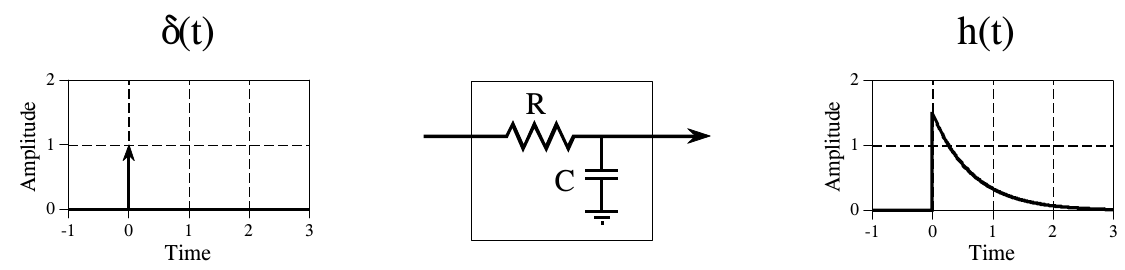
\includegraphics[width=0.938\linewidth,height=0.8\textheight,keepaspectratio]{assets/ch13/fig13-04.png}
\caption*{\textbf{图 13-4　连续线性系统的例子。}
这个电子电路是由一个电阻和一个电容组成的低通滤波器。该系统的冲激响应是一个单边指数。
（Amplitude = 幅度，Time = 时间；R = 电阻，C = 电容。）}
\end{figure}

其中 \(\alpha = 1/RC\)（R 以欧姆为单位，C 以法拉为单位，t
以秒为单位）。和离散情形一样，连续冲激响应包含了系统的全部信息，即它对一切可能信号的反应。把这个例子继续下去，图
13-5 展示了一个方波脉冲进入这个系统，用数学表示为：

\[x(t) = 1 \qquad 0 \le t \le 1\]

\[x(t) = 0 \qquad \text{其他}\]

\begin{figure}[htbp]
\centering
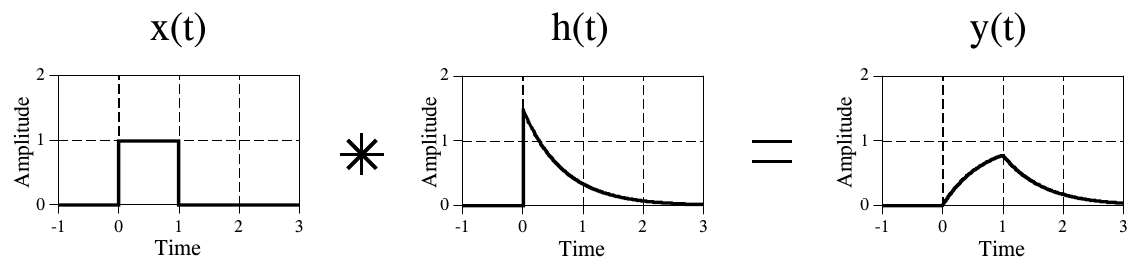
\includegraphics[width=0.946\linewidth,height=0.8\textheight,keepaspectratio]{assets/ch13/fig13-05.png}
\caption*{\textbf{图 13-5　连续卷积的例子。} 本图展示一个方波脉冲进入 RC
低通滤波器（图 13-4）。方波脉冲与系统的冲激响应卷积，得到输出。
（Amplitude = 幅度，Time = 时间。）}
\end{figure}

由于输入信号和冲激响应都已完全用数学表达式给出，输出信号 y(t)
就可以通过计算公式 13-1
的卷积积分求出。麻烦在于，两个信号都是分段定义的，而不是一个统一的数学表达式。这在连续信号处理中非常常见。通常必须画一张图，看清
t 取不同值时两个信号怎样相互滑过。在本例中，图 13-6a 表明，当 t
\textless{} 0 时两个信号完全不重叠。这意味着两个信号的乘积沿 τ
轴处处为零，得到的输出信号是：

\[y(t) = 0 \qquad t < 0\]

\begin{figure}[htbp]
\centering
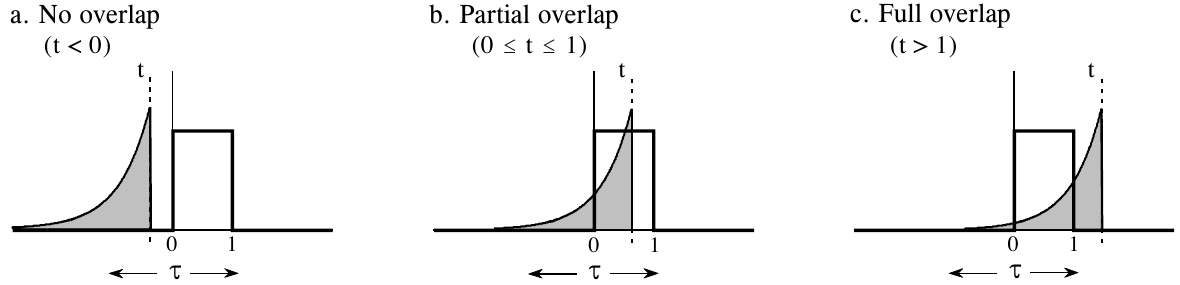
\includegraphics[width=0.983\linewidth,height=0.8\textheight,keepaspectratio]{assets/ch13/fig13-06.png}
\caption*{\textbf{图 13-6　分段计算卷积。}
由于许多连续信号是分段定义的，卷积计算也必须一段一段地做。本例中，输出信号的计算分成三段：输入信号与翻转平移后的冲激响应
(a) 不重叠，(b) 部分重叠，(c) 完全重叠。 （a. No overlap = 不重叠 (t
\textless{} 0)；b. Partial overlap = 部分重叠 (0 \dspsym{≤} t \dspsym{≤}
1)；c.~Full overlap = 完全重叠 (t \textgreater{} 1)。）}
\end{figure}

第二种情况见 (b)，此时 t 在 0 和 1 之间。两个信号部分重叠，它们的乘积在
τ = 0 到 τ = t
之间不为零。既然这是唯一的非零区域，积分只需在这一段上计算。这样得到 0
\dspsym{≤} t \dspsym{≤} 1 时的输出信号：

\[
\begin{aligned}
y(t) &= \int_{-\infty}^{\infty} x(\tau)\, h(t-\tau)\, d\tau && \text{（从公式 13-1 出发）}\\
y(t) &= \int_{0}^{t} 1\cdot \alpha e^{-\alpha(t-\tau)}\, d\tau && \text{（代入信号）}\\
y(t) &= e^{-\alpha t}\,\Big[e^{\alpha\tau}\Big]_{0}^{t} && \text{（计算积分）}\\
y(t) &= e^{-\alpha t}\,\big[e^{\alpha t} - 1\big] && \text{（化简）}\\
y(t) &= 1 - e^{-\alpha t} && 0 \le t \le 1
\end{aligned}
\]

\begin{enumerate}
\def\labelenumi{(\alph{enumi})}
\setcounter{enumi}{2}
\tightlist
\item
  给出了输出信号第三段（t \textgreater{} 1）的计算。这时重叠发生在 τ = 0
  到 τ = 1 之间，计算与第二段相同，只是积分上下限变了：
\end{enumerate}

\[
\begin{aligned}
y(t) &= \int_{0}^{1} 1\cdot \alpha e^{-\alpha(t-\tau)}\, d\tau && \text{（代入公式 13-1）}\\
y(t) &= e^{-\alpha t}\,\Big[e^{\alpha\tau}\Big]_{0}^{1} && \text{（计算积分）}\\
y(t) &= \big[e^{\alpha} - 1\big]\, e^{-\alpha t} && t > 1
\end{aligned}
\]

这三段的波形应该和你的电子学知识吻合：(1)
输入信号变为非零之前，输出信号必须为零，也就是说，第一段为 y(t) = 0，t
\textless{} 0。(2) 阶跃出现时，RC 电路按指数上升去追赶输入，方程为
\(y(t) = 1 - e^{-\alpha t}\)。(3)
输入回到零时，输出按指数衰减趋于零，方程为
\(y(t) = k e^{-\alpha t}\)（其中
\(k = e^{\alpha} - 1\)，即开始放电前一刻电容上的电压）。

更复杂的波形也可以用同样的方法处理，只是数学的复杂度会迅速变得难以驾驭。面对一个棘手的连续卷积问题时，你需要花相当多的时间评估解题策略。如果一上来就盲目地算积分，很可能最后得到一团数学乱麻。一个常用策略是把其中一个信号拆成几个更简单的相加分量，分别做卷积。利用线性原理，把得到的各个波形加起来，就是原问题的答案。

图 13-7
展示了另一种策略：以某种线性方式修改其中一个信号，做卷积，再撤销原来的修改。在这个例子里，修改是求导，撤销则是积分。单位幅度方波脉冲的导数是两个冲激：第一个面积为一，第二个面积为负一。要理解这一点，可以想想反过来对这两个冲激求积分的过程。积分经过第一个冲激时，迅速从零升到一，即一个阶跃函数。经过那个负冲激后，信号的积分又迅速从一回到零，方波脉冲就完整了。

求导之所以能简化这个问题，是因为当其中一个信号由冲激组成时，卷积很容易。x′(t)
中的两个冲激各自向输出信号的导数 y′(t)
贡献一个经过缩放和平移的冲激响应。也就是说，一眼就能看出：\(y'(t) = h(t) - h(t-1)\)。然后代入
h(t) 的确切方程，再对表达式积分，就得到输出信号 y(t)。

\begin{figure}[htbp]
\centering
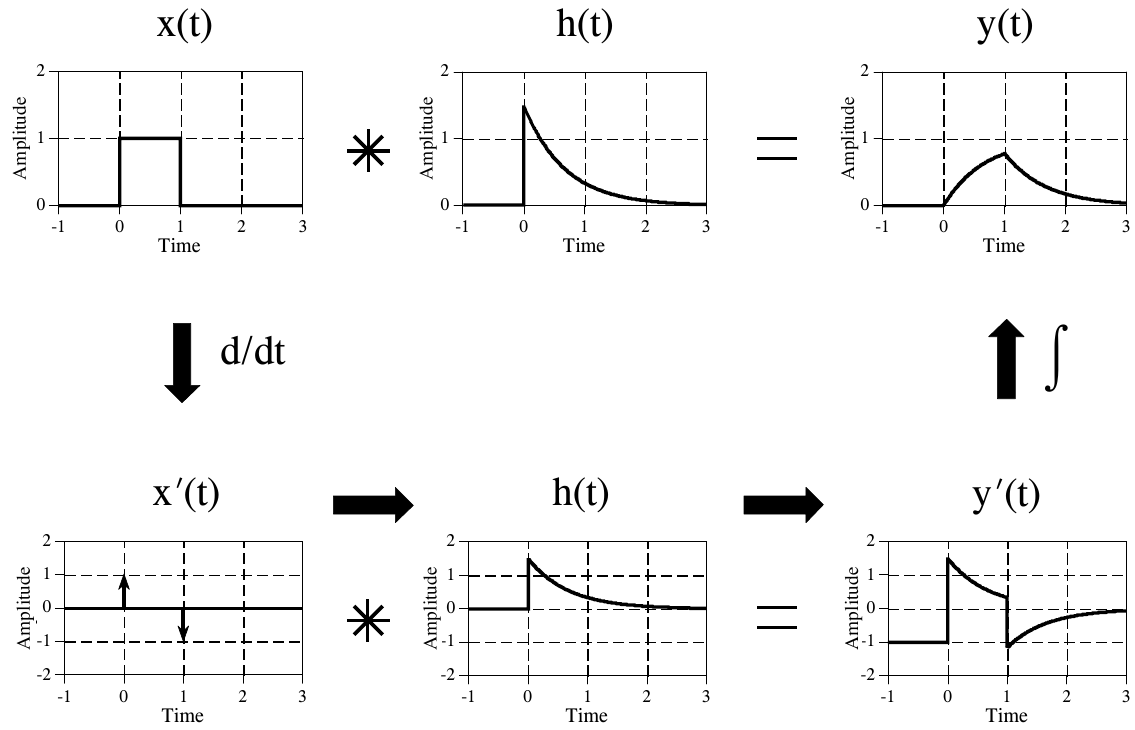
\includegraphics[width=0.946\linewidth,height=0.8\textheight,keepaspectratio]{assets/ch13/fig13-07.png}
\caption*{\textbf{图 13-7　一种卷积信号的策略。}
巧妙地运用线性系统的规则，常常能简化卷积问题。本例中，先对其中一个信号求导，从而简化两个信号的卷积。卷积完成后，再积分撤销求导。
（Amplitude = 幅度，Time = 时间；d/dt = 求导，\dspsym{∫} =
积分，\dspsym{∗} = 卷积。）}
\end{figure}

这个方法有一点小麻烦：求导时丢掉了输入信号的直流值(DC
value)。这可能导致算出的输出信号直流值有误。在数学上，这体现为积分时可以加上一个任意常数。没有系统的方法能识别这个误差，但通常可以通过检查问题来纠正。例如，图
13-7 的例子里就没有直流误差。之所以知道这一点，是因为 t
变得很大时，算出的输出信号有正确的直流值。如果某个问题中存在误差，就手动给输出信号加上一个合适的直流项来完成计算。

这个方法也适用于求几次导数后能化为冲激的信号。按这个领域的行话，这类信号叫分段多项式(piecewise
polynomial)。卷积之后，用多次积分撤销最初的多次求导。唯一的麻烦是，每一步都要找到正确的积分常数，把丢掉的直流值补回来。

在动手解一个困难的连续卷积问题之前，还有一种方法值得考虑。问问自己：输出信号真的需要一个数学表达式吗？还是有一张波形图就够了？如果一张图就够了，你也许最好用离散技术来处理这个问题，也就是用采样来近似连续信号，再用计算机程序直接做卷积。这样做虽然在数学上不那么纯粹，却可能容易得多。

\section{傅里叶变换}

连续信号的傅里叶变换分成两类：一类针对周期信号，一类针对非周期信号。周期信号使用的傅里叶变换版本叫傅里叶级数(Fourier
Series)，下一节讨论。用于非周期信号的就简单地叫傅里叶变换(Fourier
Transform)。和前几章讲离散信号时一样，本章只用实数数学来描述这些傅里叶技术。更强大的复数数学留到第
31 章。

图 13-8
是一个连续非周期信号及其频谱的例子。时域信号从负无穷延伸到正无穷，而频域的各个信号从零延伸到正无穷。这里的频谱用直角坐标形式（实部和虚部）表示；不过对连续信号也会用极坐标形式（幅度和相位）。和离散情形一样，合成方程(synthesis
equation)给出了用频域数据构造时域信号的配方。数学形式为：

\textbf{公式 13-2}　傅里叶变换合成方程。式中 x(t) 是被合成的时域信号，Re
X(ω) 和 Im X(ω) 分别是频谱的实部和虚部。

\[x(t) = \frac{1}{\pi}\int_{0}^{+\infty} \Big[\operatorname{Re}X(\omega)\cos(\omega t) - \operatorname{Im}X(\omega)\sin(\omega t)\Big]\, d\omega\]

用文字说，时域信号由无穷多个经过缩放的正弦和余弦波相加（借助积分）而成。频域的实部是余弦波的缩放系数，虚部是正弦波的缩放系数。和离散信号一样，合成方程通常写成带负号的正弦波。虽然这个负号在这里的讨论中没有意义，但它是让记法与第
31
章介绍的复数数学相容所必需的。要记住的关键一点是：有的作者在方程里加这个负号，有的不加。

\begin{quote}
\textbf{译注：} 原文此处写''第 29 章介绍的复数数学''，与本段前文''留到第
31 章''矛盾。本书讲复数 DFT 的是第 31 章，第 29 章是《DSP
上手实践》，这里按第 31 章译。
\end{quote}

还要注意，频率用符号 ω（希腊字母 omega
的小写）表示。你可能还记得，这种记法叫自然频率(natural
frequency)，单位是弧度每秒。也就是说，\(\omega = 2\pi f\)，其中 f
是以周每秒（赫兹）为单位的频率。用解方程的方式做信号处理的数学家和其他人偏爱自然频率记法，因为通常要写的符号更少。

\begin{figure}[htbp]
\centering
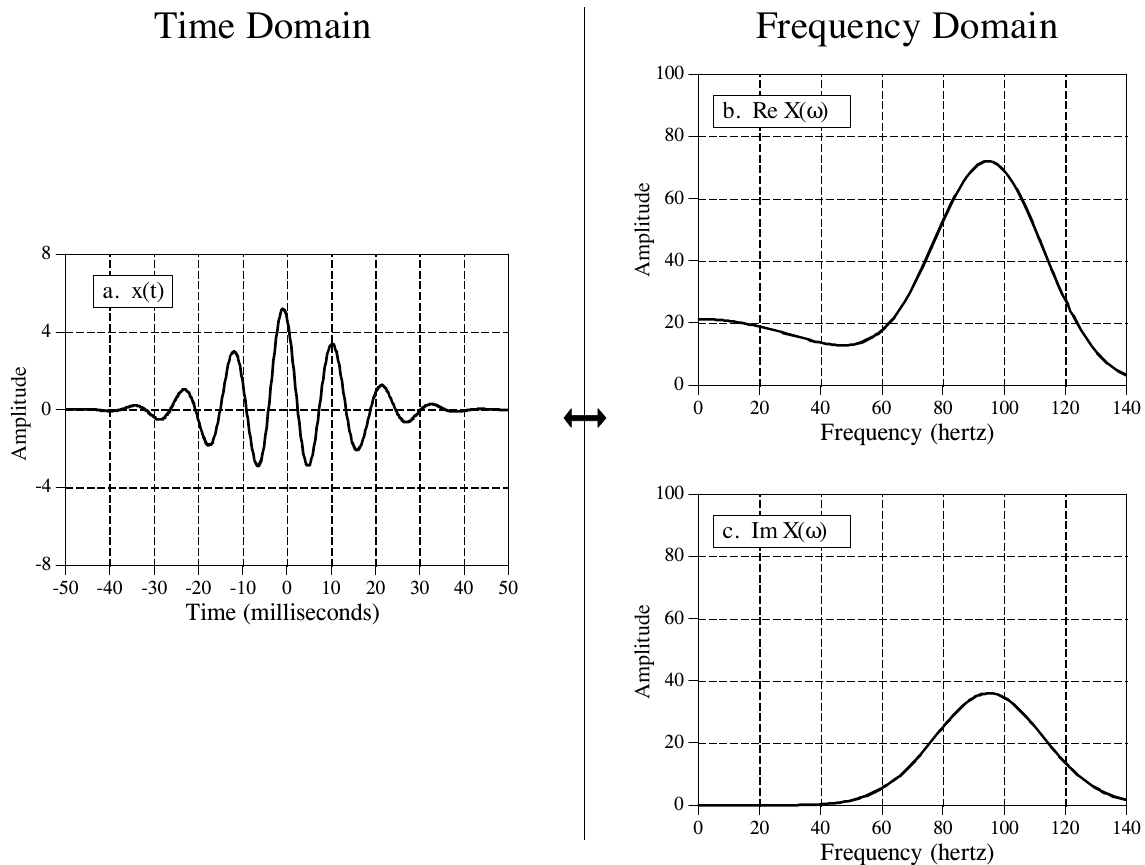
\includegraphics[width=0.954\linewidth,height=0.8\textheight,keepaspectratio]{assets/ch13/fig13-08.png}
\caption*{\textbf{图 13-8　傅里叶变换的例子。} 时域信号 x(t)
从负无穷延伸到正无穷。频域由实部 Re X(ω) 和虚部 Im X(ω)
组成，各自从零延伸到正无穷。本图的频率轴以周每秒（赫兹）标注。要换算成自然频率，把频率轴上的数乘以
2π。 （Time Domain = 时域，Frequency Domain = 频域；Amplitude =
幅度，Time (milliseconds) = 时间（毫秒），Frequency (hertz) =
频率（赫兹）。）}
\end{figure}

连续信号的分析方程(analysis
equation)沿用离散情形的思路：与正弦和余弦波做相关。方程为：

\textbf{公式 13-3}　傅里叶变换分析方程。式中 Re X(ω) 和 Im X(ω)
分别是频谱的实部和虚部，x(t) 是被分析的时域信号。

\[\operatorname{Re}X(\omega) = \int_{-\infty}^{+\infty} x(t)\cos(\omega t)\, dt\]

\[\operatorname{Im}X(\omega) = -\int_{-\infty}^{+\infty} x(t)\sin(\omega t)\, dt\]

作为使用分析方程的一个例子，我们来求 RC 低通滤波器的频率响应(frequency
response)。做法是对它的冲激响应做傅里叶变换。冲激响应前面已在图 13-4
中给出，描述为：

\[h(t) = 0 \qquad t < 0\]

\[h(t) = \alpha e^{-\alpha t} \qquad t \ge 0\]

把冲激响应代入分析方程，就能求出频率响应。先算实部：

\[
\begin{aligned}
\operatorname{Re}H(\omega) &= \int_{-\infty}^{+\infty} h(t)\cos(\omega t)\, dt && \text{（从公式 13-3 出发）}\\
\operatorname{Re}H(\omega) &= \int_{0}^{+\infty} \alpha e^{-\alpha t}\cos(\omega t)\, dt && \text{（代入信号）}\\
\operatorname{Re}H(\omega) &= \frac{\alpha e^{-\alpha t}}{\alpha^2+\omega^2}\Big[-\alpha\cos(\omega t) + \omega\sin(\omega t)\Big]_{0}^{+\infty} && \text{（计算）}\\
\operatorname{Re}H(\omega) &= \frac{\alpha^2}{\alpha^2+\omega^2}
\end{aligned}
\]

用同样的方法，算出频率响应的虚部为：

\[\operatorname{Im}H(\omega) = \frac{-\omega\alpha}{\alpha^2+\omega^2}\]

和离散信号一样，频域的直角坐标表示非常适合数学推导，却不便于人理解。把它换成极坐标就能解决这个问题，用标准关系式：\(\operatorname{Mag}H(\omega) = \big[\operatorname{Re}H(\omega)^2 + \operatorname{Im}H(\omega)^2\big]^{1/2}\)，以及
\(\operatorname{Phase}H(\omega) = \arctan\big[\operatorname{Im}H(\omega)/\operatorname{Re}H(\omega)\big]\)。

\begin{quote}
\textbf{译注：} 原文相位公式写成 arctan{[}Re H(ω) / Im
H(ω){]}，分子分母颠倒了。相位应为虚部除以实部（见第 8 章公式
8-6），下面的结果 arctan(−ω/α) 也正是按 Im/Re 算出的。
\end{quote}

经过代数运算，就得到 RC
低通滤波器以幅度和相位（即极坐标形式）表示的频率响应：

\[\operatorname{Mag}H(\omega) = \frac{\alpha}{\big[\alpha^2+\omega^2\big]^{1/2}}\]

\[\operatorname{Phase}H(\omega) = \arctan\left[-\frac{\omega}{\alpha}\right]\]

图 13-9 画出了截止频率为 1000 赫兹（即
\(\alpha = 2\pi\cdot 1000\)）时的这些曲线。

\begin{figure}[htbp]
\centering
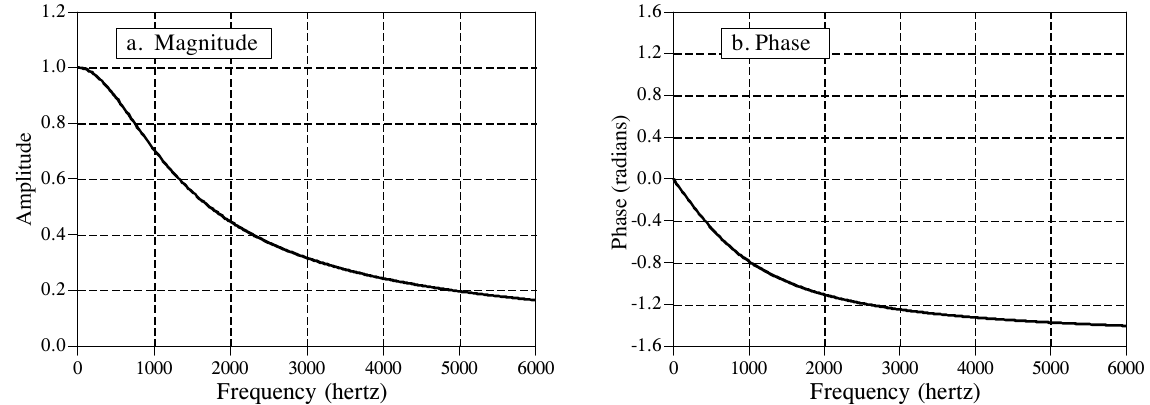
\includegraphics[width=0.958\linewidth,height=0.8\textheight,keepaspectratio]{assets/ch13/fig13-09.png}
\caption*{\textbf{图 13-9　RC 低通滤波器的频率响应。}
这些曲线是先对冲激响应做傅里叶变换，再换算成极坐标形式得到的。 （a.
Magnitude = 幅度；b. Phase = 相位。Amplitude = 幅度，Phase (radians) =
相位（弧度），Frequency (hertz) = 频率（赫兹）。）}
\end{figure}

\section{傅里叶级数}

这就讲到傅里叶变换家族的最后一位成员：傅里叶级数。傅里叶级数所用的时域信号是周期的、连续的。图
13-10 给出了几个从负无穷到正无穷不断重复的连续波形的例子。第 11
章讲过，周期信号的频谱由谐波(harmonic)组成。例如，如果时域以 1000
赫兹重复（周期 1 毫秒），频谱就会有 1000 赫兹的一次谐波、2000
赫兹的二次谐波、3000
赫兹的三次谐波，依此类推。一次谐波，即时域重复的频率，也叫基频(fundamental
frequency)。这意味着频谱可以用两种方式看待：(1)
频谱是连续的，但除谐波以外的所有频率上都为零；(2)
频谱是离散的，只在谐波频率上有定义。换句话说，谐波之间的频率可以看作取值为零，也可以看作根本不存在。重要的是，它们对形成时域信号没有贡献。

傅里叶级数合成方程把频率为 f、2f、3f、4f
等的经过缩放的余弦和正弦波加起来，构造出一个基频为 f
的连续周期信号。余弦波的幅度存放在变量 a₁、a₂、a₃、a₄
等中，正弦波的幅度存放在 b₁、b₂、b₃、b₄
等中。换句话说，``a''系数和''b''系数分别是频谱的实部和虚部。此外，系数
a₀
用来存放时域波形的直流值。它可以看作频率为零的余弦波（一个常数）的幅度。有时
a₀ 和其他''a''系数归在一起，但它常被单独处理，因为它需要特殊的计算。没有
b₀ 系数，因为频率为零的正弦波恒等于零，毫无用处。合成方程写作：

\textbf{公式 13-4}　傅里叶级数合成方程。任何周期信号 x(t)
都能由频率为基频 f 整数倍的正弦和余弦波重建出来。a\textsubscript{n} 和
b\textsubscript{n} 系数分别存放余弦波和正弦波的幅度。

\[x(t) = a_0 + \sum_{n=1}^{\infty} a_n\cos(2\pi f t n) - \sum_{n=1}^{\infty} b_n\sin(2\pi f t n)\]

傅里叶级数相应的分析方程，通常用波形的周期 T 而不是基频 f 来写（其中 f =
1/T）。由于时域信号是周期的，与正弦和余弦波的相关只需在一个周期上计算，即
−T/2 到 T/2、0 到 T、−T 到 0
等。选不同的积分限会让数学推导不同，但最终答案总是一样的。傅里叶级数分析方程为：

\textbf{公式 13-5}　傅里叶级数分析方程。式中 x(t) 是被分解的时域信号，a₀
是直流分量，a\textsubscript{n} 和 b\textsubscript{n}
分别存放余弦波和正弦波的幅度，T 是信号的周期，即基频的倒数。

\[a_0 = \frac{1}{T}\int_{-T/2}^{T/2} x(t)\, dt\]

\[a_n = \frac{2}{T}\int_{-T/2}^{T/2} x(t)\cos\!\left(\frac{2\pi t n}{T}\right) dt\]

\[b_n = \frac{-2}{T}\int_{-T/2}^{T/2} x(t)\sin\!\left(\frac{2\pi t n}{T}\right) dt\]

\begin{figure}[htbp]
\centering
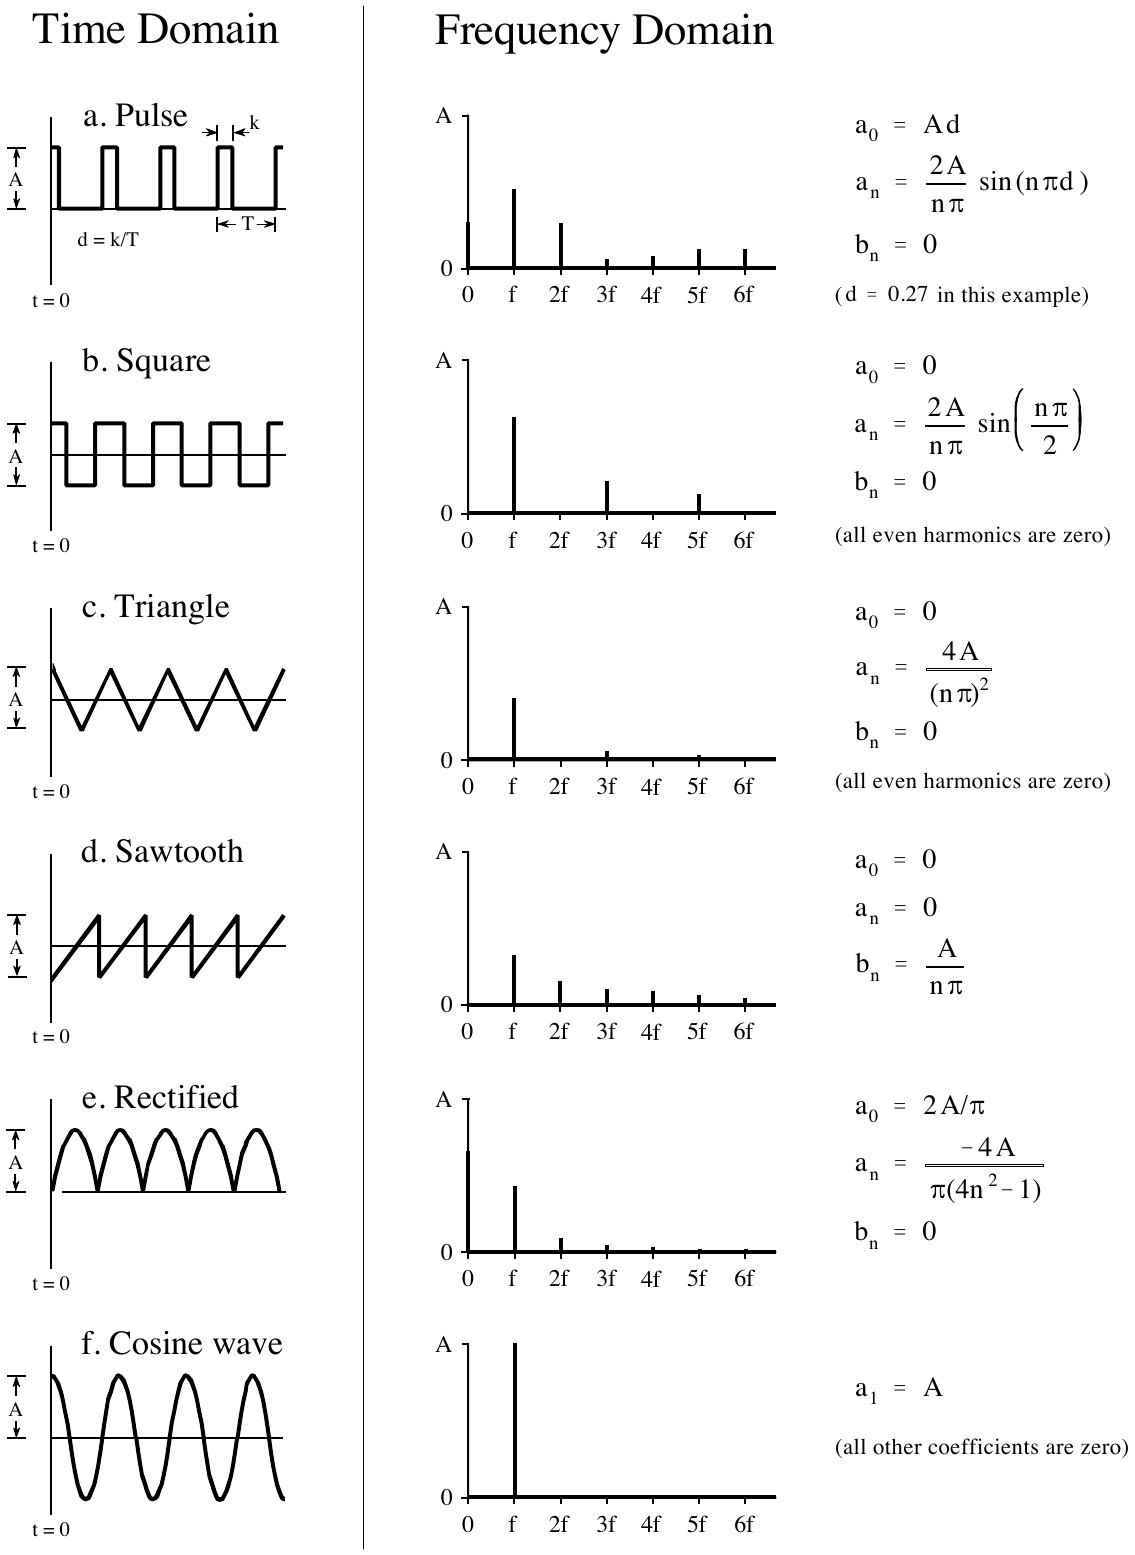
\includegraphics[width=0.946\linewidth,height=0.8\textheight,keepaspectratio]{assets/ch13/fig13-10.png}
\caption*{\textbf{图 13-10　傅里叶级数的例子。}
图中给出六种常见的时域波形，以及计算它们''a''\,``b''系数的公式。 （Time
Domain = 时域，Frequency Domain = 频域。六种波形依次为：a. Pulse =
脉冲（d = 0.27 in this example = 本例中 d = 0.27）；b. Square =
方波（all even harmonics are zero = 偶次谐波全为零）；c.~Triangle =
三角波（偶次谐波全为零）；d.~Sawtooth = 锯齿波；e. Rectified =
整流波（全波整流的正弦）；f.~Cosine wave = 余弦波（all other
coefficients are zero = 其余系数全为零）。）}
\end{figure}

图 13-11
是用这些方程计算傅里叶级数的一个例子。被分析的时域信号是一个脉冲串(pulse
train)，即高低电平持续时间不相等的方波。在 −T/2 到 T/2
的一个周期内，波形为：

\[x(t) = A \qquad -k/2 \le t \le k/2\]

\[x(t) = 0 \qquad \text{其他}\]

\begin{figure}[htbp]
\centering
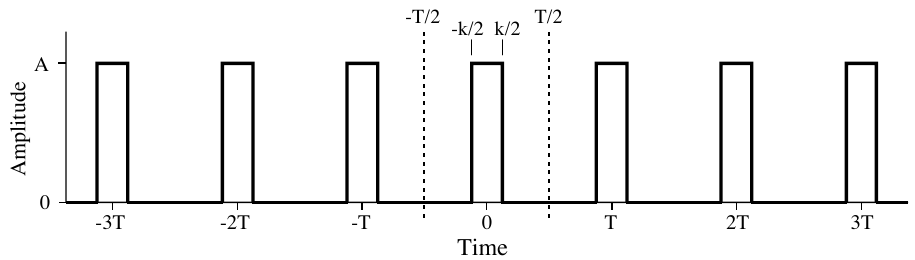
\includegraphics[width=0.762\linewidth,height=0.8\textheight,keepaspectratio]{assets/ch13/fig13-11.png}
\caption*{\textbf{图 13-11　计算傅里叶级数的例子。} 这是一个占空比 d = k/T
的脉冲串。傅里叶级数系数通过在任意一个完整周期上把波形与余弦、正弦波做相关来计算。本例用的是
−T/2 到 T/2 这个周期。 （Amplitude = 幅度，Time = 时间。）}
\end{figure}

于是波形的占空比(duty cycle，脉冲处于''高''电平的时间比例)为 d =
k/T。计算公式 13-5 就能求出傅里叶级数系数。先求直流分量 a₀：

\[
\begin{aligned}
a_0 &= \frac{1}{T}\int_{-T/2}^{T/2} x(t)\, dt && \text{（从公式 13-5 出发）}\\
a_0 &= \frac{1}{T}\int_{-k/2}^{k/2} A\, dt && \text{（代入信号）}\\
a_0 &= \frac{Ak}{T} && \text{（计算积分）}\\
a_0 &= A d && \text{（代入 d = k/T）}
\end{aligned}
\]

这个结果在直觉上说得通：直流分量就是信号的平均值。类似的分析给出''a''系数：

\[
\begin{aligned}
a_n &= \frac{2}{T}\int_{-T/2}^{T/2} x(t)\cos\!\left(\frac{2\pi t n}{T}\right) dt && \text{（从公式 13-5 出发）}\\
a_n &= \frac{2}{T}\int_{-k/2}^{k/2} A\cos\!\left(\frac{2\pi t n}{T}\right) dt && \text{（代入信号）}\\
a_n &= \frac{2A}{T}\,\frac{T}{2\pi n}\left[\sin\!\left(\frac{2\pi t n}{T}\right)\right]_{-k/2}^{k/2} && \text{（计算积分）}\\
a_n &= \frac{2A}{n\pi}\sin(\pi n d) && \text{（化简）}
\end{aligned}
\]

\begin{quote}
\textbf{译注：} 原书这组推导的第一行注明''start with Eq.
13-4''，应为公式 13-5（分析方程），上面已改正。
\end{quote}

``b''系数用同样的方法计算，不过它们全都为零。换句话说，这个波形只用余弦波就能构造出来，不需要正弦波。

如果把时域波形左右平移，``a''和''b''系数会发生变化。例如，本例中的''b''系数只有在某个脉冲以
t = 0 为中心时才为零。可以这样想：如果波形是偶的（即关于 t = 0
对称），它就只由偶的正弦型波（也就是余弦波）组成，于是所有''b''系数都为零。如果波形是奇的（即关于
t = 0
对称但符号相反），它就由奇的正弦型波（即正弦波）组成，于是''a''系数为零。如果把系数换成极坐标形式（比如
M\textsubscript{n} 和 θ\textsubscript{n}
系数），时域的平移不改变幅度，但会给相位加上一个线性分量。

为了把这个例子做完整，设想电子电路中有一个频率为 1
kHz、幅度为一伏、占空比为 0.2 的脉冲串。图 13-12
中的表格给出了这个波形所含各次谐波的幅度。图 13-12
还展示了只用前十四个谐波合成的波形。即使用了这么多谐波，重建效果也不太好。用数学行话说，傅里叶级数收敛得很慢。这只是换一种方式说：时域波形中的陡峭边沿会在频谱中产生非常高的频率。最后，一定要注意陡峭边沿处的过冲，即第
11 章讨论过的吉布斯效应(Gibbs effect)。

\begin{figure}[htbp]
\centering
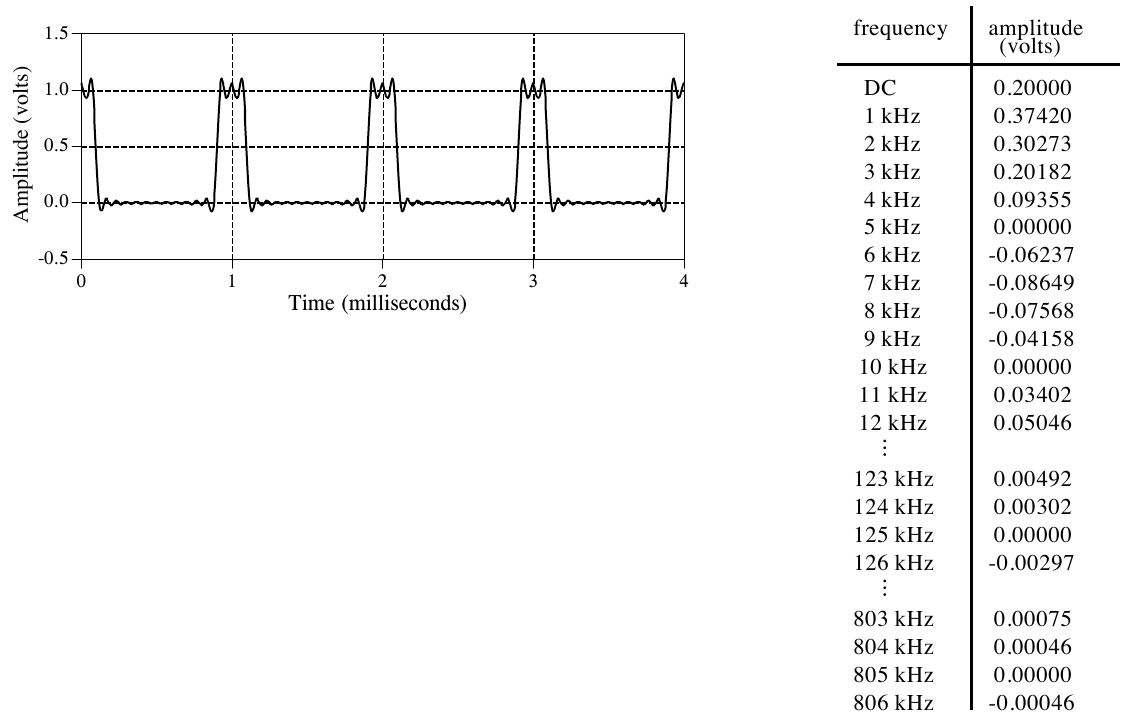
\includegraphics[width=0.942\linewidth,height=0.8\textheight,keepaspectratio]{assets/ch13/fig13-12.png}
\caption*{\textbf{图 13-12　傅里叶级数合成的例子。} 被构造的波形是一个 1
kHz、幅度一伏、占空比 0.2 的脉冲串（如图 13-11
所示）。表格列出了各次谐波的幅度，曲线图则是只用前十四个谐波重建出的波形。
（Amplitude (volts) = 幅度（伏），Time (milliseconds) =
时间（毫秒）；表头 frequency = 频率，amplitude (volts) = 幅度（伏），DC
= 直流。表中数值就是 \(a_n = \frac{2}{n\pi}\sin(0.2\pi n)\)，例如 1
kHz：\(\frac{2}{\pi}\sin(0.2\pi) \approx 0.37420\)；每到 5 的倍数 kHz
恰好为 0。）}
\end{figure}

傅里叶级数的一个重要应用是电子倍频(frequency
multiplication)。假设你要做一个非常稳定的 150 MHz
正弦波振荡器，比如工作在这个频率的无线电发射机可能就需要它。高稳定性要求电路由晶体控制，也就是说，振荡器的频率由电路中一块谐振的石英晶体决定。问题是，石英晶体只能工作到大约
10 MHz。解决办法是先做一个工作在 1～10 MHz
之间某个频率的晶控振荡器，再把频率倍增到所需的值。做法是让正弦波失真，比如用二极管削掉波峰，或者让波形通过一个平方电路。然后用带通滤波器把失真波形中的谐波分离出来。这样频率就能翻两倍、三倍，甚至乘以更高的整数。最常用的技术是用几级二倍频器和三倍频器串起来实现所需的倍频，而不是只用一级。傅里叶级数对这类设计很重要，因为它描述了倍频后信号的幅度，而这个幅度取决于失真的类型和所选的谐波。

% !TEX root = ../main.tex
% 本文件由 build-tex.sh 从 14-DSP指南-第14章中译.md 生成，改内容请改 md 后重新生成

\chapter{数字滤波器入门}\label{ch-14}

数字滤波器(digital filter)有两大用途：(1) 把混在一起的信号分开；(2)
把以某种方式失真了的信号复原。模拟（电子）滤波器也能完成同样的任务，但数字滤波器能取得好得多的效果。接下来的七章会介绍并比较最常用的数字滤波器。这一章是入门，介绍学习每种滤波器时应该关注哪些参数。

\section{滤波器基础}

数字滤波器是 DSP 中非常重要的一部分。事实上，它们出色的性能正是 DSP
变得如此流行的关键原因之一。如引言所说，滤波器有两个用途：信号分离(signal
separation)和信号复原(signal
restoration)。当一个信号被干扰、噪声或其他信号污染时，就需要信号分离。例如，设想一台测量胎儿在子宫内心脏电活动（心电图，EKG）的设备。原始信号很可能被母亲的呼吸和心跳破坏。可以用滤波器把这些信号分开，以便分别分析。

当信号以某种方式失真时，就要用信号复原。例如，用劣质设备录的音频可以经过滤波，更好地还原当时真实的声音。另一个例子是给对焦不准的镜头或抖动的相机拍到的图像去模糊。

这些问题既可以用模拟滤波器解决，也可以用数字滤波器解决。哪个更好？模拟滤波器便宜、快速，在幅度和频率上都有很大的动态范围(dynamic
range)。相比之下，数字滤波器能达到的性能水平要高得多。例如，第 16
章介绍的一个低通数字滤波器，从直流到 1000 赫兹的增益是 1 ± 0.0002，1001
赫兹以上频率的增益小于 0.0002。整个过渡只发生在 1
赫兹之内。别指望运放电路能做到这样！数字滤波器的性能可以比模拟滤波器好上千倍。这让解决滤波问题的思路发生了巨大变化。用模拟滤波器时，重点是应对电子器件的局限，比如电阻和电容的精度与稳定性。相比之下，数字滤波器好到它本身的性能常常可以不予考虑，重点转移到信号本身的局限，以及处理这些信号的理论问题上。

在 DSP 中，人们常说滤波器的输入和输出信号处在时域(time
domain)。这是因为信号通常是按相等的时间间隔采样得到的。但这不是唯一的采样方式。第二常见的方式是按相等的空间间隔采样。例如，设想沿飞机机翼的长度方向每隔一厘米装一个应变传感器，同时读取这一排传感器的读数。其他的域也有可能，但时间和空间是迄今为止最常见的。在
DSP
中看到''时域''这个词时，记住它可能真的指随时间采集的样本，也可能泛指采样所在的任何域。

如图 14-1 所示，每个线性滤波器都有一个冲激响应(impulse
response)、一个阶跃响应(step response)和一个频率响应(frequency
response)。这三者每一个都包含了关于滤波器的完整信息，只是形式不同。只要给定其中一个，另外两个就确定了，可以直接算出来。这三种表示都很重要，因为它们描述了滤波器在不同情形下会怎样反应。

实现数字滤波器最直接的方法，是把输入信号与数字滤波器的冲激响应卷积。所有可能的线性滤波器都能用这种方式做出来。（这应该是显然的。如果你不觉得显然，那你大概还不具备理解这一部分滤波器设计的基础。试着复习一下前面关于
DSP
基础的部分。）当冲激响应这样使用时，滤波器设计者给它起了个专门的名字：滤波器核(filter
kernel)。

做数字滤波器还有另一种方法，叫递归(recursion)。用卷积实现滤波器时，输出中的每个采样都是对输入采样加权后相加得到的。递归滤波器(recursive
filter)是这种做法的扩展：除了用输入中的点，还用之前已经算出的输出值。递归滤波器不用滤波器核，而是用一组递归系数(recursion
coefficients)来定义。这种方法会在第 19
章详细讨论。眼下的要点是：所有线性滤波器都有冲激响应，即使你不用它来实现滤波器。要求出递归滤波器的冲激响应，只要输入一个冲激，看看输出什么就行了。递归滤波器的冲激响应由幅度按指数衰减的正弦波组成。原则上，这使它们的冲激响应无限长。不过，幅度最终会降到系统的舍入噪声以下，剩下的采样就可以忽略。由于这个特点，递归滤波器也叫无限冲激响应(Infinite
Impulse Response)滤波器，即 IIR
滤波器。相比之下，用卷积实现的滤波器叫有限冲激响应(Finite Impulse
Response)滤波器，即 FIR 滤波器。

\begin{figure}[htbp]
\centering
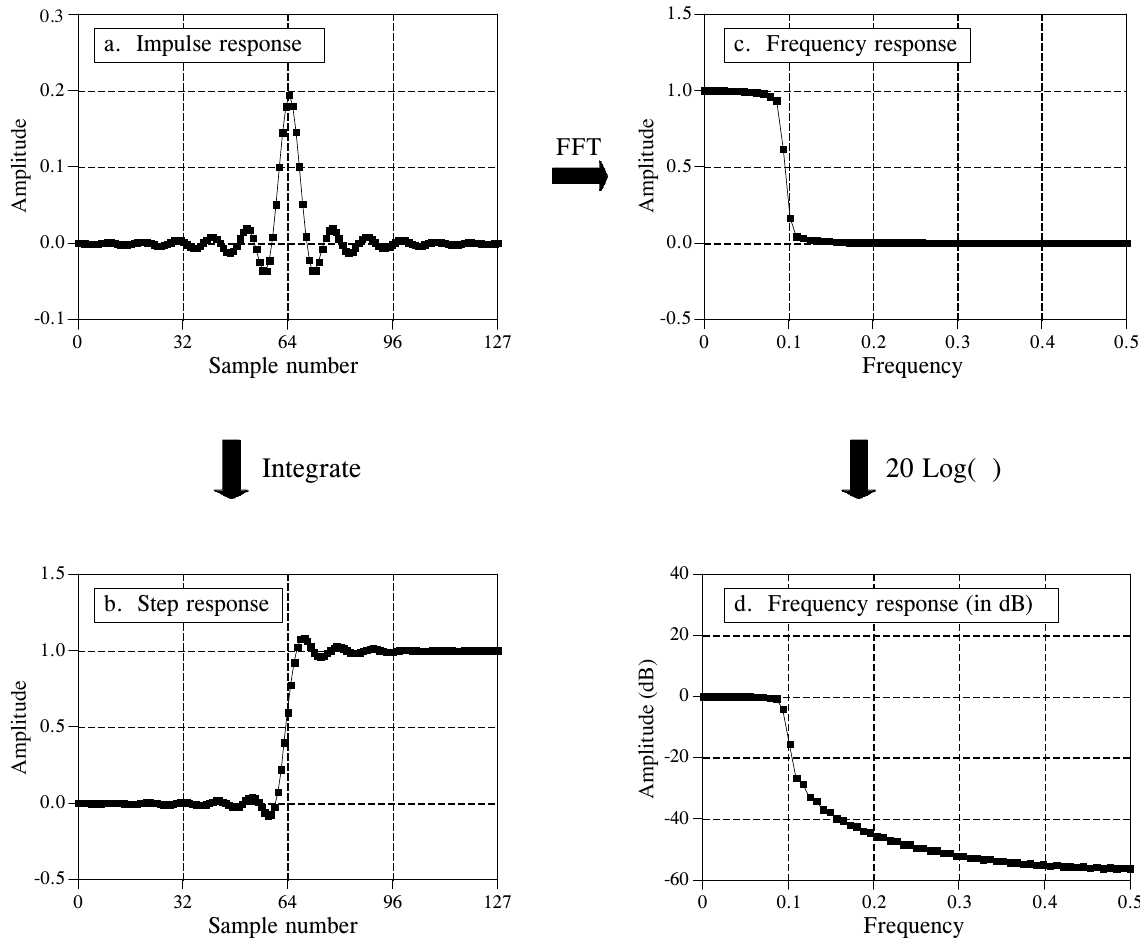
\includegraphics[width=0.950\linewidth,height=0.8\textheight,keepaspectratio]{assets/ch14/fig14-01.png}
\caption*{\textbf{图 14-1　滤波器的参数。}
每个线性滤波器都有冲激响应、阶跃响应和频率响应。阶跃响应 (b)
可以通过对冲激响应 (a)
做离散积分求得。频率响应可以用快速傅里叶变换（FFT）从冲激响应求得，既可以用线性刻度显示
(c)，也可以用分贝显示 (d)。 （a. Impulse response = 冲激响应；b. Step
response = 阶跃响应；c.~Frequency response = 频率响应；d.~Frequency
response (in dB) = 频率响应（分贝）。箭头：FFT；Integrate = 积分；20
Log( ) = 取 20 倍对数。Amplitude = 幅度，Amplitude (dB) =
幅度（分贝），Sample number = 采样序号，Frequency = 频率。）}
\end{figure}

你已经知道，冲激响应是输入为冲激时系统的输出。同样，阶跃响应是输入为阶跃(step)时的输出（阶跃也叫边沿(edge)，阶跃响应也叫边沿响应(edge
response)）。由于阶跃是冲激的积分，阶跃响应就是冲激响应的积分。这提供了两种求阶跃响应的方法：(1)
把阶跃波形送进滤波器，看输出什么；(2)
对冲激响应积分。（数学上严格地说：积分用于连续信号，而离散积分，即累加和，用于离散信号。）频率响应可以通过对冲激响应做
DFT（用 FFT
算法）求得，本章后面会复习这一点。频率响应可以画在线性纵轴上，如
(c)；也可以画在对数刻度（分贝）上，如
(d)。线性刻度最适合显示通带纹波和滚降，而要显示阻带衰减就需要分贝刻度。

记不清分贝了？这里快速复习一下。一贝尔(bel，为纪念亚历山大·格雷厄姆·贝尔而得名)表示功率变化了十倍。例如，一个放大倍数为
3 贝尔的电子电路，输出信号的功率是输入的 10 × 10 × 10 = 1000
倍。一分贝(decibel，dB)是十分之一贝尔。因此，−20dB、−10dB、0dB、10dB 和
20dB 分别对应功率比 0.01、0.1、1、10 和
100。换句话说，每十分贝表示功率变化了十倍。

问题在于：你通常想处理的是信号的幅度，而不是功率。例如，设想一个增益为
20dB 的放大器。按定义，这意味着信号的功率增大了 100
倍。由于幅度与功率的平方根成正比，输出的幅度是输入的 10 倍。20dB
在功率上意味着 100 倍，在幅度上却只意味着 10
倍。每二十分贝表示幅度变化了十倍。写成公式：

\textbf{公式
14-1}　分贝的定义。分贝是表示两个信号之比的一种方式。功率之比（P₁ 和
P₂）与幅度之比（A₁ 和 A₂）用的公式不同。

\[\text{dB} = 10\log_{10}\frac{P_2}{P_1}\]

\[\text{dB} = 20\log_{10}\frac{A_2}{A_1}\]

上面的公式用的是以 10 为底的对数，但许多计算机语言只提供以 e
为底的对数函数（自然对数，写作 \(\log_e x\) 或
\(\ln x\)）。把上面的公式改一下就能用自然对数：\(\text{dB} = 4.342945\,\log_e(P_2/P_1)\)
和 \(\text{dB} = 8.685890\,\log_e(A_2/A_1)\)。

既然分贝是表示两个信号之比的方式，它就非常适合描述系统的增益，即输出信号与输入信号之比。不过，工程师也用分贝来标定单个信号的幅度（或功率），办法是把它与某个标准作参照。例如，dBV
表示以 1 伏有效值(rms)的信号为参照。同样，dBm 表示以在 600 欧负载上产生
1 毫瓦功率的信号为参照（约 0.78 伏有效值）。

如果关于分贝你别的什么都记不住，就记住两件事。第一，−3dB 表示幅度降到
0.707（因而功率降到 0.5）。第二，背下下面这些分贝与幅度比之间的换算：

{\def\LTcaptype{none} % do not increment counter
\begin{longtable}[]{@{}rr@{}}
\toprule\noalign{}
分贝 & 幅度比 \\
\midrule\noalign{}
\endhead
\bottomrule\noalign{}
\endlastfoot
60dB & 1000 \\
40dB & 100 \\
20dB & 10 \\
0dB & 1 \\
−20dB & 0.1 \\
−40dB & 0.01 \\
−60dB & 0.001 \\
\end{longtable}
}

\section{信息在信号中是怎样表示的}

任何 DSP
任务中最重要的部分，是弄懂信息是怎样包含在你所处理的信号中的。信息包含在信号中的方式有很多种，人造信号尤其如此。比如，想想人们设计出的各种调制方案：调幅(AM)、调频(FM)、单边带(single-sideband)、脉冲编码调制(pulse-code
modulation)、脉宽调制(pulse-width
modulation)等等，不胜枚举。幸运的是，在自然产生的信号中，常见的信息表示方式只有两种。我们把它们叫做：在时域中表示的信息，和在频域中表示的信息。

在时域中表示的信息，描述的是某件事什么时候发生、发生的幅度有多大。例如，设想一个研究太阳光输出的实验。光输出每秒测量并记录一次。信号中的每个采样都表明那一刻正在发生什么，以及事件的强度。如果发生了一次太阳耀斑，信号会直接给出它发生的时间、持续时长、随时间的发展等信息。每个采样所含的信息无需参照其他采样就能解读。即使你只有这个信号的一个采样，也仍然对所测的东西有所了解。这是信息包含在信号中最简单的方式。

相比之下，在频域中表示的信息更为间接。我们宇宙中的许多事物都呈现周期运动。例如，用指甲敲一下酒杯，它会振动，发出清脆的响声；落地钟的钟摆来回摆动；恒星和行星绕自身的轴自转、又相互绕转，等等。测量这种周期运动的频率、相位和幅度，往往能获得关于产生这种运动的系统的信息。假设我们对敲响的酒杯发出的声音采样。周期振动的基频和谐波与材料的质量和弹性有关。单独一个采样本身不含有任何关于周期运动的信息，因而也不含有任何关于酒杯的信息。信息包含在信号中许多点之间的关系里。

这就引出了阶跃响应和频率响应的重要性。阶跃响应描述了在时域中表示的信息被系统怎样改变。而频率响应展示了在频域中表示的信息被怎样改变。这个区别在滤波器设计中至关重要，因为不可能让一个滤波器同时在这两种应用中都达到最优。时域性能好，就会导致频域性能差，反之亦然。如果你设计的滤波器是要去除心电图信号中的噪声（信息在时域中表示），阶跃响应就是重要参数，频率响应则无关紧要。如果你的任务是为助听器设计数字滤波器（信息在频域中），频率响应就是一切，阶跃响应则无所谓。下面来看看是什么让一个滤波器在时域或频域应用中达到最优。

\section{时域参数}

为什么时域滤波器如此关注阶跃响应，可能并不显而易见。你也许会问，为什么重要参数不是冲激响应？答案在于人的大脑理解和处理信息的方式。记住，阶跃响应、冲激响应和频率响应包含的信息完全相同，只是排列方式不同。阶跃响应之所以在时域分析中有用，是因为它契合人看待信号中所含信息的方式。

例如，假设给你一个来历不明的信号，让你分析。你做的第一件事，就是把信号划分成特征相似的若干区域。你没法不这么做，你的大脑会自动这么做。有些区域可能很平滑，有些可能有很大的幅度峰值，有些可能噪声很多。这种分段是通过找出区域之间的分界点完成的。这正是阶跃函数(step
function)发挥作用的地方。阶跃函数是表示两个不同区域之间分界的最纯粹的方式。它可以标记一个事件何时开始，或者何时结束。它告诉你左边的东西在某种程度上与右边的东西不同。这就是人脑看待时域信息的方式：一组阶跃函数把信息划分成特征相似的区域。而阶跃响应之所以重要，是因为它描述了这些分界线被滤波器怎样改变。

滤波器设计中重要的阶跃响应参数如图 14-2
所示。要分辨信号中的事件，阶跃响应的持续时间必须短于事件之间的间隔。这就要求阶跃响应尽可能地快（这是
DSP 的行话），如图 (a) 和 (b)
所示。标定上升时间(risetime，又一个行话)最常用的方法，是给出幅度从 10\%
到 90\%
之间的采样数。为什么不能总是做到非常快的上升时间？原因很多：降低噪声、数据采集系统固有的限制、避免混叠等等。

\begin{figure}[htbp]
\centering
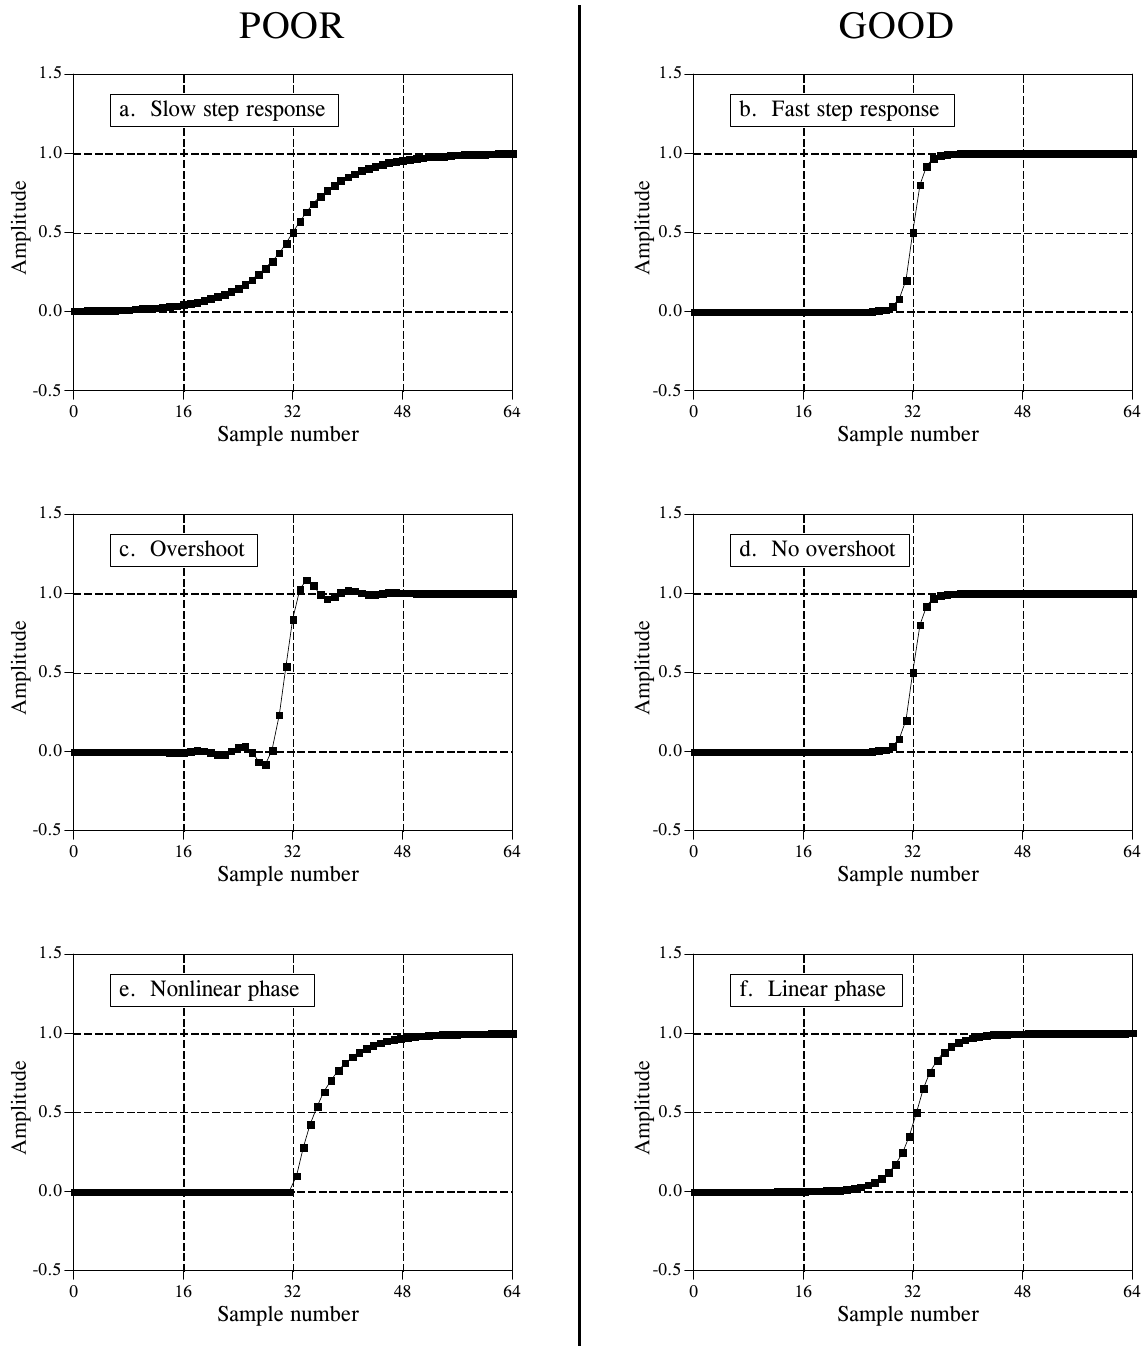
\includegraphics[width=0.954\linewidth,height=0.8\textheight,keepaspectratio]{assets/ch14/fig14-02.png}
\caption*{\textbf{图 14-2　评价时域性能的参数。}
阶跃响应用来衡量滤波器在时域中的表现。有三个参数很重要：(1)
过渡速度（上升时间），见 (a) 和 (b)；(2) 过冲，见 (c) 和 (d)；(3)
相位线性（阶跃上下两半的对称性），见 (e) 和 (f)。 （POOR = 差，GOOD =
好；a. Slow step response = 慢的阶跃响应；b. Fast step response =
快的阶跃响应；c.~Overshoot = 过冲；d.~No overshoot = 无过冲；e.
Nonlinear phase = 非线性相位；f.~Linear phase = 线性相位。Amplitude =
幅度，Sample number = 采样序号。）}
\end{figure}

图 (c) 和 (d)
展示了下一个重要参数：阶跃响应中的过冲(overshoot)。过冲一般必须消除，因为它改变了信号中采样的幅度，这是对时域中所含信息的一种根本性失真。这可以归结为一个问题：你在信号中看到的过冲，是来自你要测量的东西，还是来自你用的滤波器？

最后，人们常常希望阶跃响应的上半部分与下半部分对称，如 (e) 和 (f)
所示。需要这种对称性，才能让上升沿和下降沿看起来一样。这种对称叫线性相位(linear
phase)，因为频率响应的相位是一条直线（第 19
章讨论）。务必理解这三个参数，它们是评价时域滤波器的关键。

\section{频域参数}

图 14-3
展示了四种基本的频率响应。这些滤波器的目的，是让某些频率原封不动地通过，同时完全挡住另一些频率。通带(passband)指被通过的那些频率，阻带(stopband)包含被挡住的那些频率，过渡带(transition
band)在两者之间。滚降(roll-off)快，意味着过渡带非常窄。通带与过渡带的分界叫截止频率(cutoff
frequency)。在模拟滤波器设计中，截止频率通常定义为幅度降到 0.707（即
−3dB）的位置。数字滤波器的标准化程度没那么高，常见到把幅度降到
99\%、90\%、70.7\% 和 50\% 的位置定义为截止频率。

\begin{figure}[htbp]
\centering
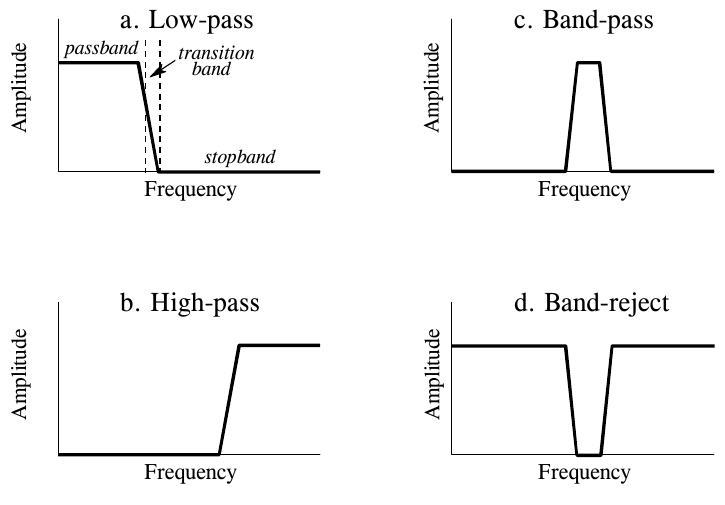
\includegraphics[width=0.604\linewidth,height=0.8\textheight,keepaspectratio]{assets/ch14/fig14-03.png}
\caption*{\textbf{图 14-3　四种常见的频率响应。}
频域滤波器一般用来让某些频率通过（通带），同时挡住另一些频率（阻带）。最常见的四种响应是：低通、高通、带通和带阻。
（a. Low-pass = 低通；b. High-pass = 高通；c.~Band-pass =
带通；d.~Band-reject = 带阻；passband = 通带，transition band =
过渡带，stopband = 阻带。Amplitude = 幅度，Frequency =
频率。原书这段图注排在图的左侧，裁图时已去掉，译文见上。）}
\end{figure}

图 14-4
展示了衡量滤波器频域性能的三个参数。要分开靠得很近的频率，滤波器必须滚降快，如
(a) 和 (b)
所示。要让通带频率原封不动地通过滤波器，就必须没有通带纹波(passband
ripple)，如 (c) 和 (d)
所示。最后，要充分挡住阻带频率，就需要良好的阻带衰减(stopband
attenuation)，如 (e) 和 (f) 所示。

\begin{figure}[htbp]
\centering
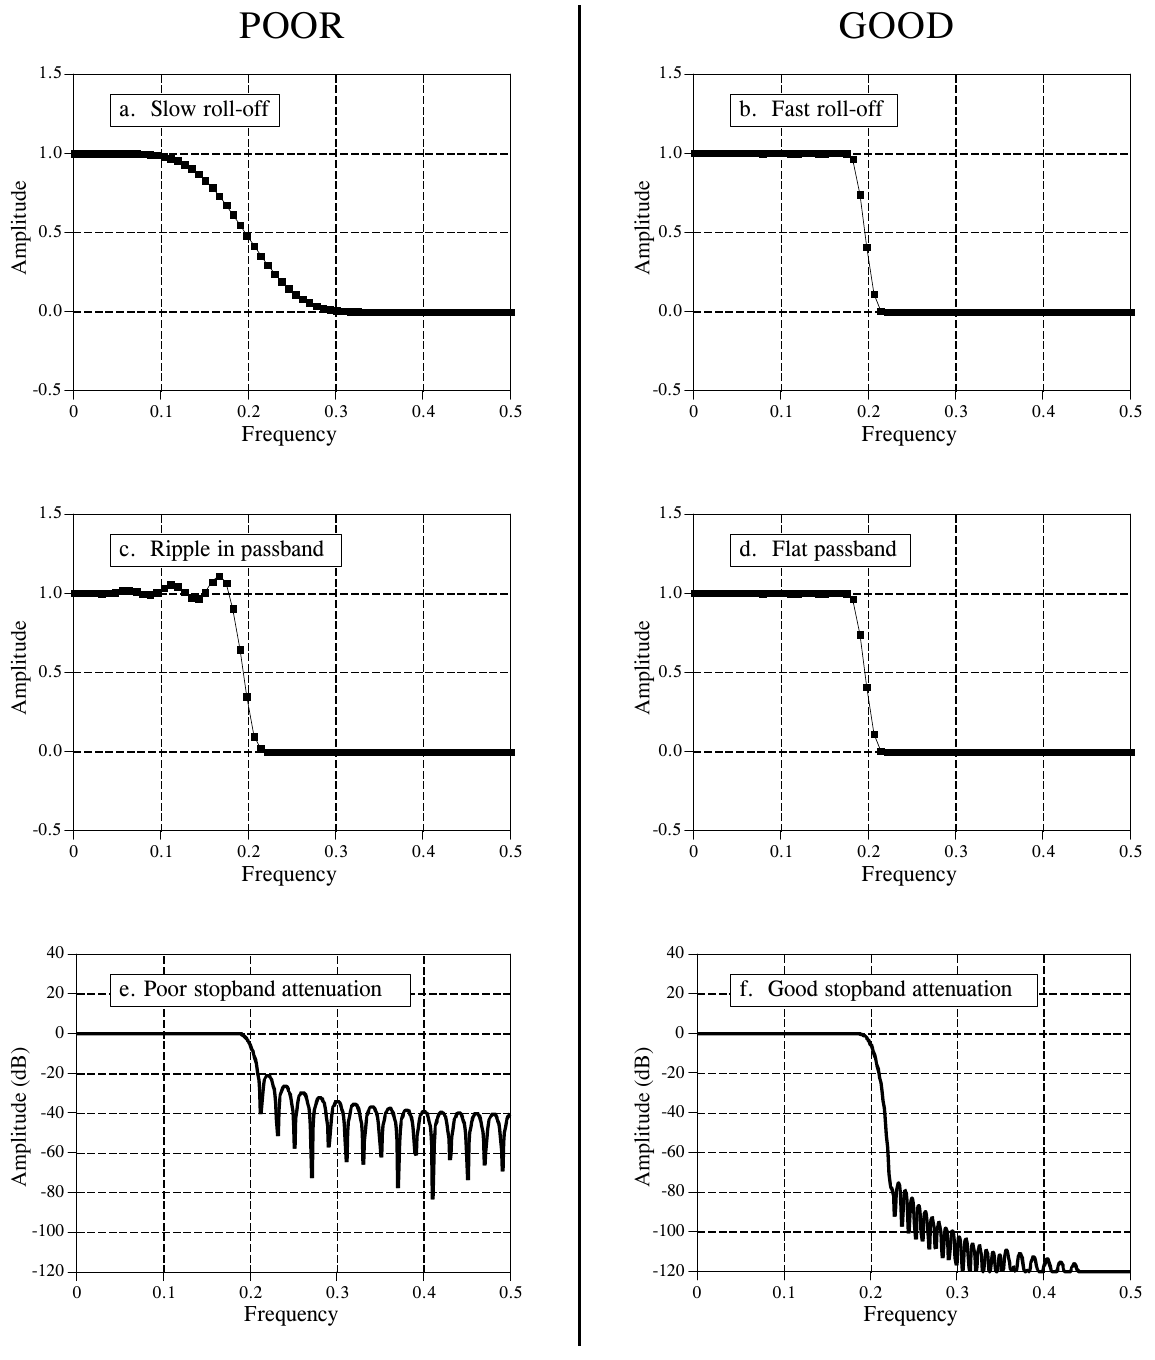
\includegraphics[width=0.963\linewidth,height=0.8\textheight,keepaspectratio]{assets/ch14/fig14-04.png}
\caption*{\textbf{图 14-4　评价频域性能的参数。}
图中的频率响应都是低通滤波器的。有三个参数很重要：(1) 滚降的陡峭程度，见
(a) 和 (b)；(2) 通带纹波，见 (c) 和 (d)；(3) 阻带衰减，见 (e) 和 (f)。
（POOR = 差，GOOD = 好；a. Slow roll-off = 滚降慢；b. Fast roll-off =
滚降快；c.~Ripple in passband = 通带有纹波；d.~Flat passband =
通带平坦；e. Poor stopband attenuation = 阻带衰减差；f.~Good stopband
attenuation = 阻带衰减好。Amplitude = 幅度，Amplitude (dB) =
幅度（分贝），Frequency = 频率。）}
\end{figure}

为什么这些参数里没有一个和相位有关？第一，在大多数频域应用中，相位并不重要。例如，音频信号的相位几乎完全是随机的，不含多少有用的信息。第二，如果相位很重要，做出相位响应完美的数字滤波器也非常容易，即所有频率通过滤波器时相移都为零（同样在第
19 章讨论）。相比之下，模拟滤波器在这方面糟糕透顶。

前面几章讲过 DFT
怎样把系统的冲激响应转换成频率响应。这里简单复习一下。计算 DFT
最快的方法是用第 12 章介绍的 FFT 算法。从一个 N 点长的滤波器核出发，FFT
算出的频谱由 N 点实部和 N 点虚部组成。FFT 实部和虚部中只有第 0 到第 N/2
个采样含有有用的信息，其余的点是重复的（负频率），可以忽略。由于实部和虚部人很难看懂，通常把它们转换成第
8 章介绍的极坐标形式。这就得到幅度信号和相位信号，各自从第 0 个采样到第
N/2 个采样（即每个信号有 N/2 + 1 个采样）。例如，256
点的冲激响应会得到从第 0 点到第 128 点的频率响应。第 0
个采样代表直流，即零频率；第 128
个采样代表采样率的一半。记住，采样数据中不可能出现高于采样率一半的频率。

用来表示冲激响应的采样数可以任意多。例如，假设你想求一个由 80
个点组成的滤波器核的频率响应。由于 FFT 只能处理长度为 2
的幂的信号，你需要给信号补 48 个零，使它长 128
个采样。补零不会改变冲激响应。要理解为什么，想想输入信号与系统冲激响应卷积时，这些补上的零会怎样：它们在卷积中直接消失，不影响结果。

更进一步，你可以给冲激响应补很多零，让它长达比如 256、512 或 1024
点。重要的一点是：冲激响应越长，频率响应中数据点的间距就越密。也就是说，在直流到采样率一半之间分布的采样更多。推到极致，如果给冲激响应补无穷多个零，频率响应中的数据点就无限接近，成为一条连续的线。换句话说，滤波器的频率响应实际上是直流到采样率一半之间的一个连续信号，DFT
的输出是对这条连续曲线的采样。计算滤波器的频率响应时，冲激响应该取多长？第一个念头可以试
N = 1024，但如果需要（比如分辨率不够或计算时间太长），别怕改。

记住，本章讨论的''好''与''坏''参数只是笼统的概括。许多信号并不能整整齐齐地归入某一类。例如，想想一个被
60
赫兹干扰污染的心电图信号。信息编码在时域中，但干扰最好在频域中处理。这种应用的最佳设计必然要有所取舍，而且可能和本章的常规观点相悖。记住教育的头号法则：书上的一段话并不是让你停止思考的许可证。

\section{高通、带通和带阻滤波器}

高通(high-pass)、带通(band-pass)和带阻(band-reject)滤波器的设计方法，是先设计一个低通(low-pass)滤波器，再把它转换成需要的响应。正因为如此，大多数关于滤波器设计的讨论只举低通滤波器的例子。从低通到高通的转换有两种方法：频谱反转(spectral
inversion)和频谱翻转(spectral reversal)。两种方法同样有用。

图 14-5 是频谱反转的一个例子。图 (a) 是一个叫加窗 sinc(windowed-sinc，第
16 章的主题)的低通滤波器核。这个滤波器核长 51
点，不过很多采样的值非常小，在这张图里看上去像是零。对应的频率响应如 (b)
所示，是给滤波器核补 13 个零、做 64 点 FFT
得到的。把低通滤波器核变成高通滤波器核要做两件事：第一，把滤波器核中每个采样的符号取反；第二，在对称中心的采样上加一。这样就得到
(c) 中的高通滤波器核，其频率响应如 (d)
所示。频谱反转把频率响应上下翻转，通带变成阻带，阻带变成通带。换句话说，它把滤波器从低通变成高通、高通变成低通、带通变成带阻、或者带阻变成带通。

\begin{figure}[htbp]
\centering
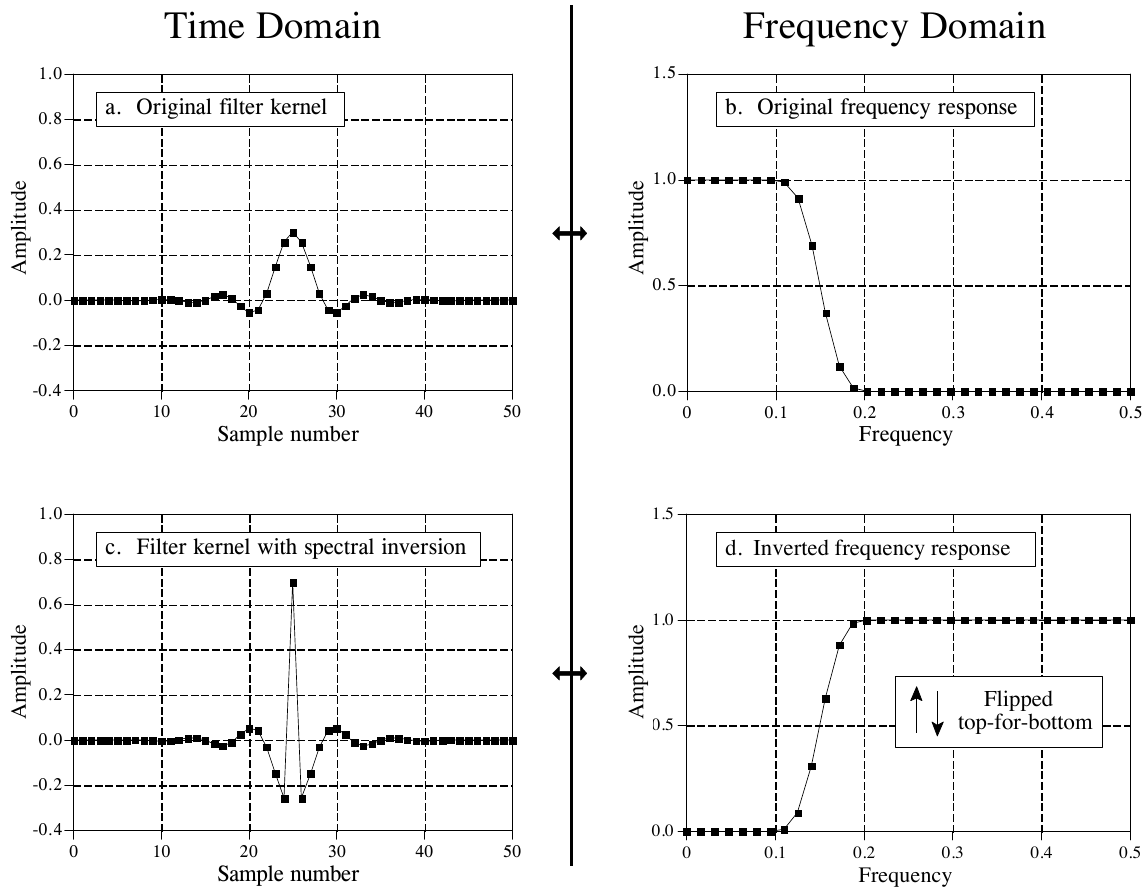
\includegraphics[width=0.954\linewidth,height=0.8\textheight,keepaspectratio]{assets/ch14/fig14-05.png}
\caption*{\textbf{图 14-5　频谱反转的例子。} (a) 中低通滤波器核的频率响应如 (b)
所示。把 (a)
中每个采样的符号取反，再在对称中心的采样上加一，就得到高通滤波器核
(c)。时域中的这一操作使频谱反转（即上下翻转），得到 (d)
所示的高通频率响应。 （Time Domain = 时域，Frequency Domain = 频域；a.
Original filter kernel = 原滤波器核；b. Original frequency response =
原频率响应；c.~Filter kernel with spectral inversion =
频谱反转后的滤波器核；d.~Inverted frequency response =
反转后的频率响应；Flipped top-for-bottom = 上下翻转。Amplitude =
幅度，Sample number = 采样序号，Frequency = 频率。）}
\end{figure}

图 14-6 说明了为什么时域中的这两步修改会使频谱反转。在 (a) 中，输入信号
x{[}n{]} 同时送入两个并联的系统。其中一个是低通滤波器，冲激响应为
h{[}n{]}。另一个对信号什么都不做，因此其冲激响应是一个冲激函数
δ{[}n{]}。总输出 y{[}n{]}
等于全通系统的输出减去低通系统的输出。由于低频成分从原信号中被减掉了，输出中只剩下高频成分。这样就构成了一个高通滤波器。

\begin{figure}[htbp]
\centering
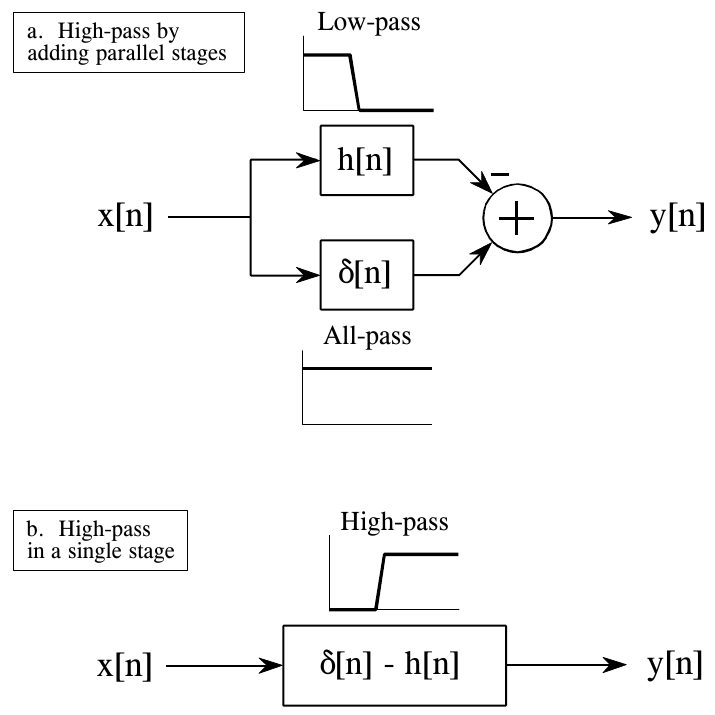
\includegraphics[width=0.596\linewidth,height=0.8\textheight,keepaspectratio]{assets/ch14/fig14-06.png}
\caption*{\textbf{图 14-6　频谱反转的框图。} 在 (a) 中，输入信号 x{[}n{]}
送入两个并联的系统，它们的冲激响应分别为 h{[}n{]} 和 δ{[}n{]}。如 (b)
所示，组合后系统的冲激响应为 δ{[}n{]} −
h{[}n{]}。这意味着组合系统的频率响应是 h{[}n{]} 频率响应的反转。 （a.
High-pass by adding parallel stages = 用并联相加的方式得到高通；b.
High-pass in a single stage = 单级高通；Low-pass = 低通，All-pass =
全通，High-pass = 高通；加法器上的 −
号表示减去该支路。原书这段图注排在图的左侧，裁图时已去掉，译文见上。）}
\end{figure}

这在计算机程序中可以分两步完成：让信号通过一个低通滤波器，再从原信号中减去滤波后的信号。不过，把两个滤波器核合并起来，整个操作可以在单级中完成。第
7 章讲过，输出相加的并联系统可以通过把冲激响应相加合并成单级。如 (b)
所示，高通滤波器的滤波器核为 δ{[}n{]} −
h{[}n{]}。也就是说，把所有采样的符号取反，再在对称中心的采样上加一。

\begin{quote}
\textbf{译注：} 原文此处写作 ``performed in a signal stage''，应为
``single stage''（单级），按后者译出。
\end{quote}

要让这个技巧奏效，从低通滤波器出来的低频成分，必须与从全通系统出来的低频成分相位相同，否则就无法完全相减。这给方法加上了两条限制：(1)
原滤波器核必须左右对称（即零相位或线性相位）；(2)
冲激必须加在对称中心处。

从低通到高通的第二种方法是频谱翻转，如图 14-7 所示。和前面一样，(a)
中的低通滤波器核对应 (b) 中的频率响应。把 (a)
中每隔一个的采样取反，就得到高通滤波器核 (c)。如 (d)
所示，这使频域左右翻转：0 变成 0.5，0.5 变成
0。示例低通滤波器的截止频率是 0.15，因此高通滤波器的截止频率是 0.35。

\begin{figure}[htbp]
\centering
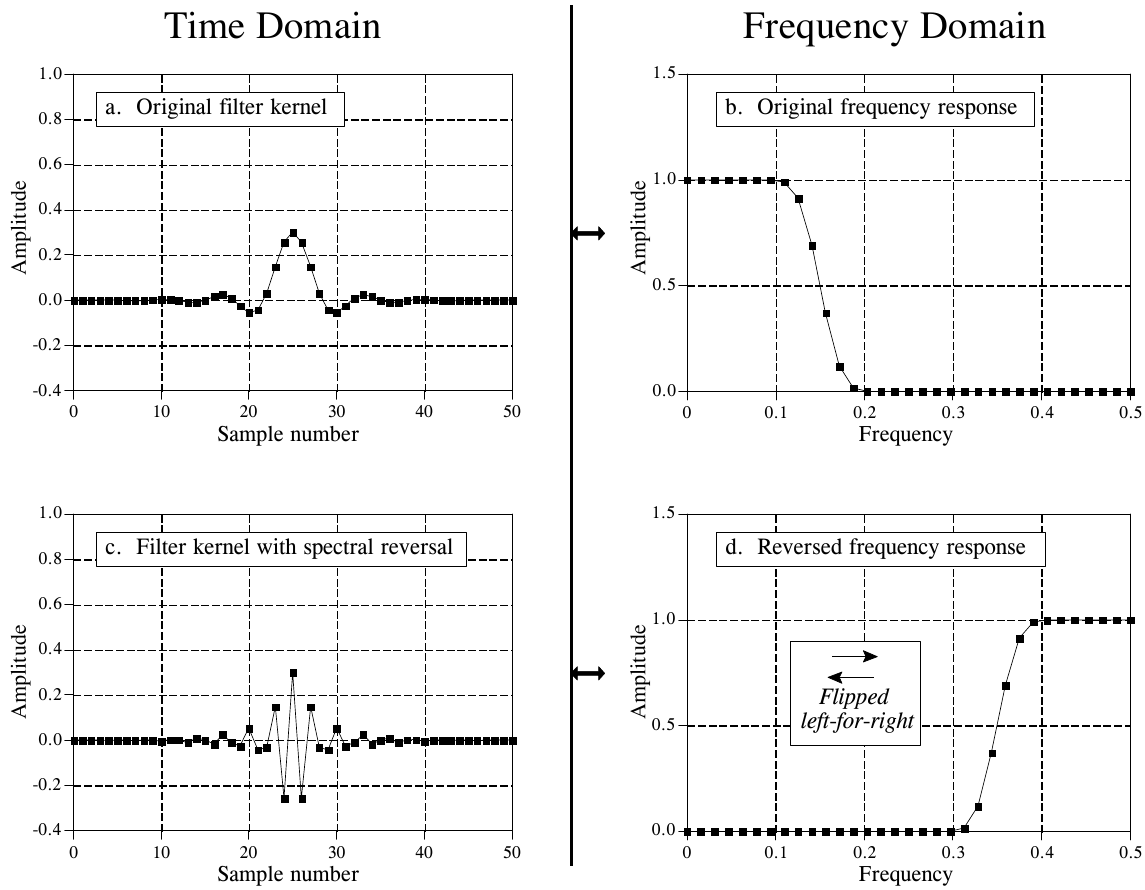
\includegraphics[width=0.954\linewidth,height=0.8\textheight,keepaspectratio]{assets/ch14/fig14-07.png}
\caption*{\textbf{图 14-7　频谱翻转的例子。} (a) 中低通滤波器核的频率响应如 (b)
所示。把 (a) 中每隔一个的采样取反，就得到高通滤波器核
(c)。时域中的这一操作使频域左右翻转，得到 (d) 所示的高通频率响应。
（Time Domain = 时域，Frequency Domain = 频域；a. Original filter kernel
= 原滤波器核；b. Original frequency response = 原频率响应；c.~Filter
kernel with spectral reversal = 频谱翻转后的滤波器核；d.~Reversed
frequency response = 翻转后的频率响应；Flipped left-for-right =
左右翻转。Amplitude = 幅度，Sample number = 采样序号，Frequency =
频率。）}
\end{figure}

把每隔一个的采样取反，等价于把滤波器核乘以一个频率为 0.5 的正弦波。第 10
章讲过，这会使频域平移 0.5。看着 (b)，想象 −0.5 到 0
之间的负频率，它们是 0 到 0.5 之间频率的镜像。(d) 中出现的频率，正是 (b)
中的负频率平移 0.5 之后的结果。

最后，图 14-8 和 14-9
展示了怎样把低通和高通滤波器核组合成带通和带阻滤波器。简单地说，把滤波器核相加得到带阻滤波器，把滤波器核卷积得到带通滤波器。这依据的是第
7
章讨论过的级联系统和并联系统的合并方式。这些技巧也可以多次组合使用。例如，可以先把两个滤波器核相加，构成一个带阻滤波器，再用前面讲的频谱反转或频谱翻转，就设计出了一个带通滤波器。所有这些技巧都非常好用，很少会有意外。

\begin{quote}
\textbf{译注：} 原文把相加得到的滤波器写作 ``stop-pass
filter''，按上下文就是带阻(band-reject)滤波器，译文直接译作带阻。
\end{quote}

\begin{figure}[htbp]
\centering
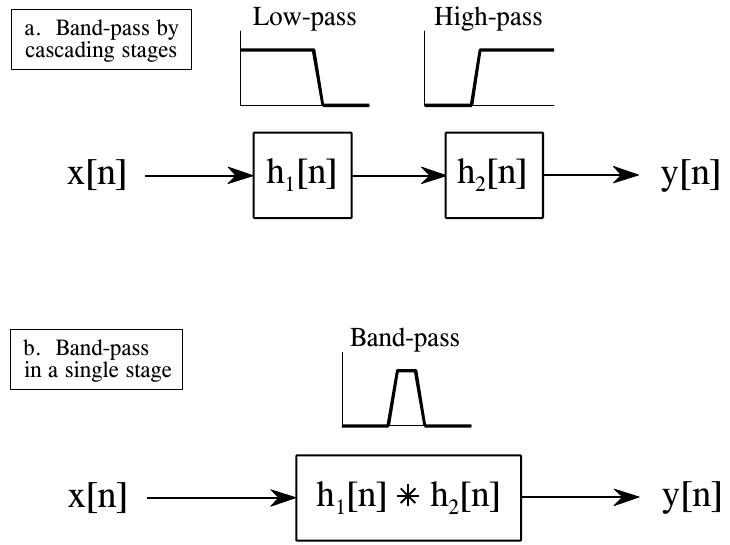
\includegraphics[width=0.608\linewidth,height=0.8\textheight,keepaspectratio]{assets/ch14/fig14-08.png}
\caption*{\textbf{图 14-8　设计带通滤波器。} 如 (a)
所示，把一个低通滤波器和一个高通滤波器级联，就能构成带通滤波器。这可以化简为
(b) 所示的单级，单级的滤波器核等于低通和高通滤波器核的卷积。 （a.
Band-pass by cascading stages = 用级联得到带通；b. Band-pass in a single
stage = 单级带通；Low-pass = 低通，High-pass = 高通，Band-pass =
带通；方框里的 \dspsym{∗}
是卷积。原书这段图注排在图的左侧，裁图时已去掉，译文见上。）}
\end{figure}

\begin{figure}[htbp]
\centering
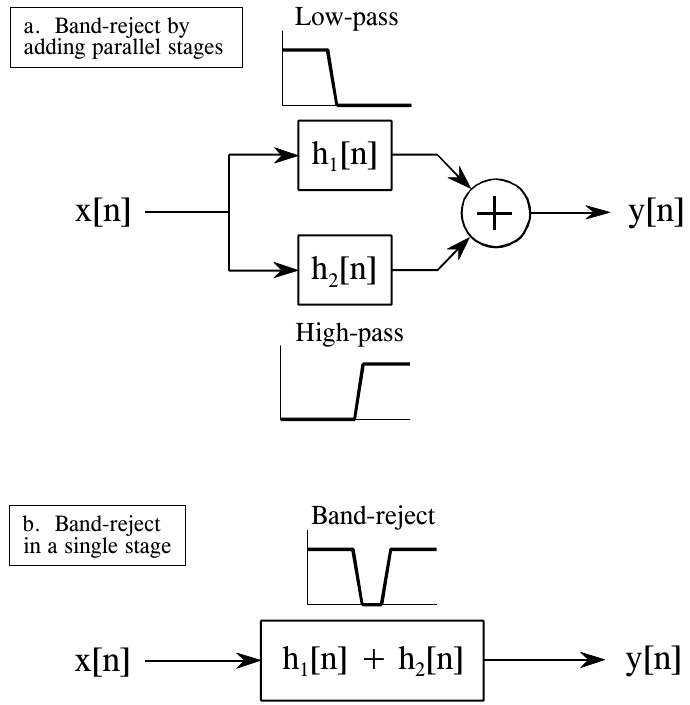
\includegraphics[width=0.575\linewidth,height=0.8\textheight,keepaspectratio]{assets/ch14/fig14-09.png}
\caption*{\textbf{图 14-9　设计带阻滤波器。} 如 (a)
所示，把一个低通滤波器和一个高通滤波器并联、输出相加，就构成带阻滤波器。图
(b) 是化简后的单级，其滤波器核等于低通和高通滤波器核之和。 （a.
Band-reject by adding parallel stages = 用并联相加得到带阻；b.
Band-reject in a single stage = 单级带阻；Low-pass = 低通，High-pass =
高通，Band-reject =
带阻。原书这段图注排在图的左侧，裁图时已去掉，译文见上。）}
\end{figure}

\section{滤波器的分类}

表 14-1
总结了数字滤波器怎样按用途和实现方式分类。数字滤波器的用途可分为三类：时域、频域和定制(custom)。如前所述，当信息编码在信号波形的形状中时，用时域滤波器。时域滤波用于平滑、去直流、波形整形等操作。相比之下，当信息包含在各正弦分量的幅度、频率和相位中时，用频域滤波器。这类滤波器的目标是把一个频带与另一个频带分开。当需要滤波器完成某种特殊操作、比四种基本响应（高通、低通、带通和带阻）更复杂的事情时，就用定制滤波器。例如，第
17
章介绍怎样用定制滤波器做反卷积(deconvolution)，这是抵消一次不想要的卷积的一种方法。

\textbf{表 14-1　滤波器的分类。} 滤波器可以按用途和实现方式划分。

{\def\LTcaptype{none} % do not increment counter
\begin{longtable}[]{@{}
  >{\raggedright\arraybackslash}p{(\linewidth - 4\tabcolsep) * \real{0.3333}}
  >{\raggedright\arraybackslash}p{(\linewidth - 4\tabcolsep) * \real{0.3333}}
  >{\raggedright\arraybackslash}p{(\linewidth - 4\tabcolsep) * \real{0.3333}}@{}}
\toprule\noalign{}
\begin{minipage}[b]{\linewidth}\raggedright
滤波器用于 ＼ 滤波器实现方式
\end{minipage} & \begin{minipage}[b]{\linewidth}\raggedright
卷积\\
有限冲激响应（FIR）\strut
\end{minipage} & \begin{minipage}[b]{\linewidth}\raggedright
递归\\
无限冲激响应（IIR）\strut
\end{minipage} \\
\midrule\noalign{}
\endhead
\bottomrule\noalign{}
\endlastfoot
\textbf{时域}（平滑、去直流） & 移动平均（第 15 章） & 单极点（第 19
章） \\
\textbf{频域}（分离频率） & 加窗 sinc（第 16 章） & 切比雪夫（第 20
章） \\
\textbf{定制}（反卷积） & FIR 定制（第 17 章） & 迭代设计（第 26 章） \\
\end{longtable}
}

（原表英文：FILTER USED FOR = 滤波器用于，FILTER IMPLEMENTED BY =
滤波器实现方式；Convolution = 卷积，Recursion = 递归；Moving average =
移动平均(moving average)，Single pole = 单极点(single
pole)，Windowed-sinc = 加窗 sinc，Chebyshev = 切比雪夫(Chebyshev)，FIR
custom = FIR 定制，Iterative design = 迭代设计(iterative design)。）

数字滤波器可以用两种方式实现：卷积（也叫有限冲激响应，FIR）和递归（也叫无限冲激响应，IIR）。用卷积实现的滤波器性能可以远好于用递归实现的滤波器，但执行起来慢得多。

接下来的六章按照表 14-1
的分类介绍数字滤波器。首先看用卷积实现的滤波器。移动平均（第 15
章）用于时域，加窗 sinc（第 16 章）用于频域，FIR 定制（第 17
章）用于需要特殊处理的场合。为了结束对 FIR 滤波器的讨论，第 18
章介绍一种叫 FFT 卷积的技术。这是一种提高卷积速度的算法，能让 FIR
滤波器执行得更快。

接着看递归滤波器。单极点递归滤波器（第 19
章）用于时域，而切比雪夫滤波器（第 20
章）用于频域。具有定制响应的递归滤波器要用迭代技术来设计。因此，我们把它们的讨论推迟到第
26 章，在那里和另一种迭代方法------神经网络(neural
network)------一起介绍。

如表 14-1
所示，卷积和递归是相互竞争的技术，在具体应用中你只能选其一。怎么选？第
21 章会在时域和频域两方面对二者做正面比较。

% !TEX root = ../main.tex
% 本文件由 build-tex.sh 从 15-DSP指南-第15章中译.md 生成，改内容请改 md 后重新生成

\chapter{移动平均滤波器}\label{ch-15}

移动平均(moving average)是 DSP
中最常用的滤波器，主要因为它是最容易理解和使用的数字滤波器。别看它简单，移动平均滤波器对一项常见任务却是最优的：在保持阶跃响应陡峭的同时降低随机噪声。这使它成为时域编码信号(time
domain encoded signal)的首选滤波器。然而，对于频域编码信号(frequency
domain encoded
signal)，移动平均是最差的滤波器，几乎没有能力把一个频带与另一个频带分开。移动平均滤波器的亲戚包括高斯(Gaussian)滤波器、布莱克曼(Blackman)滤波器和多次移动平均(multiple-pass
moving average)滤波器。它们在频域的表现稍好一些，代价是计算时间更长。

\section{用卷积实现}

顾名思义，移动平均滤波器的做法是：把输入信号中若干个点取平均，得到输出信号中的每一个点。写成公式：

\textbf{公式 15-1}　移动平均滤波器的公式。式中 x{[} {]} 是输入信号，y{[}
{]} 是输出信号，M
是参与平均的点数。这个公式只用到正在计算的输出采样一侧的点。

\[y[i] = \frac{1}{M} \sum_{j=0}^{M-1} x[i+j]\]

其中 x{[} {]} 是输入信号，y{[} {]} 是输出信号，M 是平均的点数。例如，在
5 点移动平均滤波器中，输出信号的第 80 点由下式给出：

\[y[80] = \frac{x[80] + x[81] + x[82] + x[83] + x[84]}{5}\]

另一种做法是，从输入信号中围绕输出点对称地选取这组点：

\[y[80] = \frac{x[78] + x[79] + x[80] + x[81] + x[82]}{5}\]

这相当于把公式 15-1 中的求和范围从 \(j = 0\) 到 \(M-1\) 改成
\(j = -(M-1)/2\) 到 \((M-1)/2\)。例如，在 11 点移动平均滤波器中，下标 j
可以从 0 到 10（单侧平均），也可以从 −5 到 5（对称平均）。对称平均要求 M
是奇数。只取一侧的点编程稍微容易一点，但会使输入和输出信号之间产生相对平移。

\begin{quote}
\textbf{译注：} 原书这里写 ``from 0 to 11''，11 点的单侧下标应为 0 到
10，译文已改正。
\end{quote}

你应该看出来了，移动平均滤波器就是用一个非常简单的滤波器核做卷积。例如，5
点滤波器的滤波器核是：\dspsym{⋯} 0, 0, 1/5, 1/5, 1/5, 1/5, 1/5, 0, 0
\dspsym{⋯}。也就是说，移动平均滤波器就是输入信号与一个面积为一的矩形脉冲(rectangular
pulse)做卷积。表 15-1 是实现移动平均滤波器的程序。

\textbf{表 15-1}（注释已译成中文）

\begin{Shaded}
\begin{Highlighting}[]
\NormalTok{100 \textquotesingle{}MOVING AVERAGE FILTER}
\NormalTok{110 \textquotesingle{}这个程序用 101 点移动平均滤波器处理 5000 个采样，}
\NormalTok{120 \textquotesingle{}得到 4900 个滤波后的数据。}
\NormalTok{130 \textquotesingle{}}
\NormalTok{140 DIM X[4999]                        \textquotesingle{}X[ ] 存放输入信号}
\NormalTok{150 DIM Y[4999]                        \textquotesingle{}Y[ ] 存放输出信号}
\NormalTok{160 \textquotesingle{}}
\NormalTok{170 GOSUB XXXX                         \textquotesingle{}虚构的子程序，载入 X[ ]}
\NormalTok{180 \textquotesingle{}}
\NormalTok{190 FOR I\% = 50 TO 4949                \textquotesingle{}遍历输出信号的每个点}
\NormalTok{200 Y[I\%] = 0                          \textquotesingle{}清零，用作累加器}
\NormalTok{210 FOR J\% = {-}50 TO 50                 \textquotesingle{}计算求和}
\NormalTok{220 Y[I\%] = Y[I\%] + X(I\%+J\%]}
\NormalTok{230 NEXT J\%}
\NormalTok{240 Y[I\%] = Y[I\%]/101                  \textquotesingle{}除以点数，完成平均}
\NormalTok{250 NEXT I\%}
\NormalTok{260 \textquotesingle{}}
\NormalTok{270 END}
\end{Highlighting}
\end{Shaded}

\begin{quote}
\textbf{译注：} 第 220 行原书印成
\texttt{X(I\%+J\%{]}}，左右括号不配对，应为 \texttt{X{[}I\%+J\%{]}}。
\end{quote}

\textbf{C 实现}（完整可编译版本见
\texttt{c/table15-1\_moving\_average.c}，其中按图 15-1a
的样子生成信号：幅度 1 的矩形脉冲埋在标准差 0.5 的高斯白噪声里）：

\begin{Shaded}
\begin{Highlighting}[]
\PreprocessorTok{\#define N    }\DecValTok{5000}\PreprocessorTok{                           }\CommentTok{/* 140 DIM X[4999]：输入 5000 点 */}
\PreprocessorTok{\#define HALF }\DecValTok{50}\PreprocessorTok{                             }\CommentTok{/* 210：J\% 从 {-}50 到 50，共 101 点 */}
\PreprocessorTok{\#define M    }\OperatorTok{(}\DecValTok{2}\PreprocessorTok{ }\OperatorTok{*}\PreprocessorTok{ HALF }\OperatorTok{+}\PreprocessorTok{ }\DecValTok{1}\OperatorTok{)}

\CommentTok{/* 190～250：每个输出点取输入中以它为中心的 101 点求平均 */}
\DataTypeTok{static} \DataTypeTok{void}\NormalTok{ moving\_average}\OperatorTok{(}\DataTypeTok{const} \DataTypeTok{float} \OperatorTok{*}\NormalTok{x}\OperatorTok{,} \DataTypeTok{float} \OperatorTok{*}\NormalTok{y}\OperatorTok{)}
\OperatorTok{\{}
    \ControlFlowTok{for} \OperatorTok{(}\DataTypeTok{int}\NormalTok{ i }\OperatorTok{=} \DecValTok{0}\OperatorTok{;}\NormalTok{ i }\OperatorTok{\textless{}}\NormalTok{ N}\OperatorTok{;}\NormalTok{ i}\OperatorTok{++)}\NormalTok{ y}\OperatorTok{[}\NormalTok{i}\OperatorTok{]} \OperatorTok{=} \FloatTok{0.0}\BuiltInTok{f}\OperatorTok{;} \CommentTok{/* 两端 50 点没有完整窗口，不计算，置 0 */}
    \ControlFlowTok{for} \OperatorTok{(}\DataTypeTok{int}\NormalTok{ i }\OperatorTok{=}\NormalTok{ HALF}\OperatorTok{;}\NormalTok{ i }\OperatorTok{\textless{}}\NormalTok{ N }\OperatorTok{{-}}\NormalTok{ HALF}\OperatorTok{;}\NormalTok{ i}\OperatorTok{++)} \OperatorTok{\{} \CommentTok{/* 190：FOR I\% = 50 TO 4949 */}
\NormalTok{        y}\OperatorTok{[}\NormalTok{i}\OperatorTok{]} \OperatorTok{=} \FloatTok{0.0}\BuiltInTok{f}\OperatorTok{;}                        \CommentTok{/* 200：清零，当累加器用 */}
        \ControlFlowTok{for} \OperatorTok{(}\DataTypeTok{int}\NormalTok{ j }\OperatorTok{=} \OperatorTok{{-}}\NormalTok{HALF}\OperatorTok{;}\NormalTok{ j }\OperatorTok{\textless{}=}\NormalTok{ HALF}\OperatorTok{;}\NormalTok{ j}\OperatorTok{++)} \CommentTok{/* 210：FOR J\% = {-}50 TO 50 */}
\NormalTok{            y}\OperatorTok{[}\NormalTok{i}\OperatorTok{]} \OperatorTok{+=}\NormalTok{ x}\OperatorTok{[}\NormalTok{i }\OperatorTok{+}\NormalTok{ j}\OperatorTok{];}               \CommentTok{/* 220：原书印成 X(I\%+J\%]，括号不配对 */}
\NormalTok{        y}\OperatorTok{[}\NormalTok{i}\OperatorTok{]} \OperatorTok{/=}\NormalTok{ M}\OperatorTok{;}                          \CommentTok{/* 240：除以 101 完成平均 */}
    \OperatorTok{\}}
\OperatorTok{\}}
\end{Highlighting}
\end{Shaded}

运行结果：平坦区的噪声标准差从 0.4905 降到 0.0500，降低 9.81
倍，与理论值 \dspsym{√}101 \dspsym{≈} 10.05
相符；去掉噪声后，脉冲上升沿从第 1950 点离开 0、第 2050 点到达 1，正好
101 点，中点 y{[}2000{]} = 0.5050 = 51/101，即阶跃响应是一条直线。

\section{降噪与阶跃响应}

许多科学家和工程师用移动平均滤波器时会有负罪感。因为它实在太简单，遇到问题时往往第一个就拿它来试。即使问题已经完全解决，心里还是觉得应该再多做点什么。这种情形实在很讽刺。移动平均滤波器不仅在许多应用中表现很好，而且对一个常见问题是最优的：在保持最陡阶跃响应的同时降低随机白噪声(random
white noise)。

\begin{figure}[htbp]
\centering
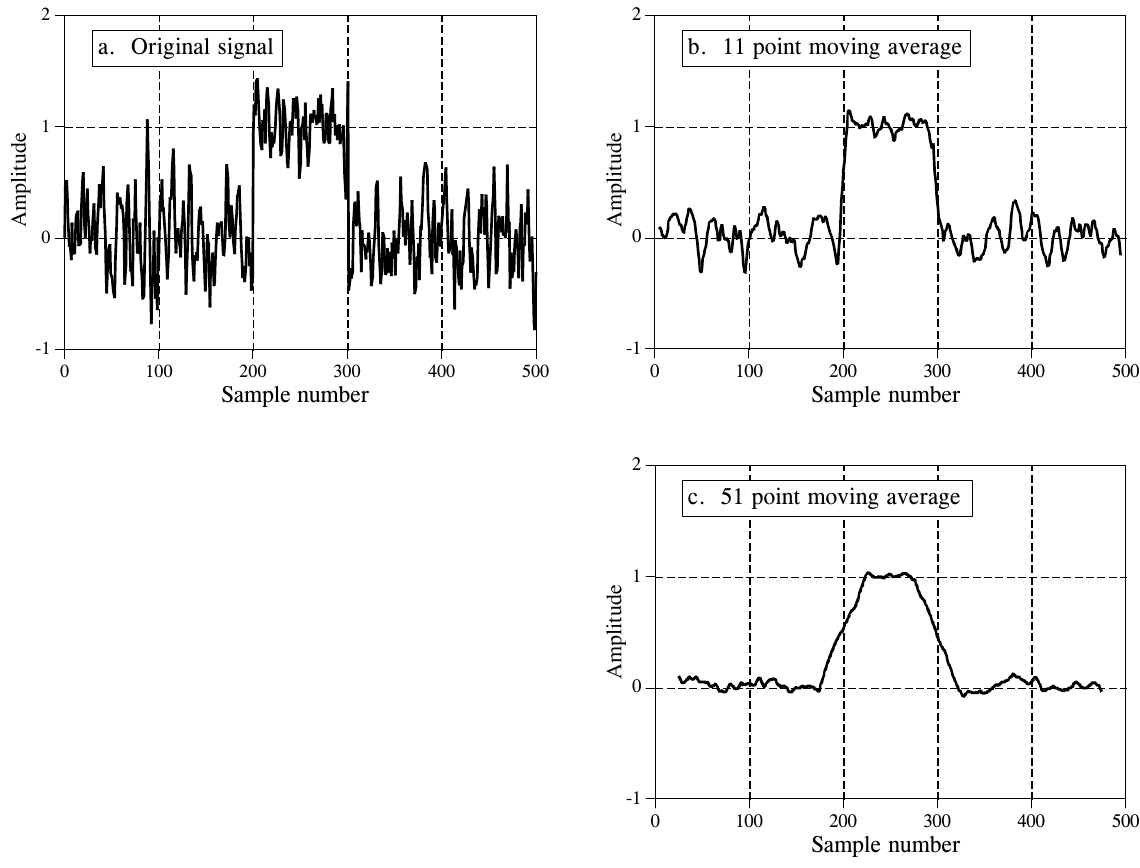
\includegraphics[width=0.950\linewidth,height=0.8\textheight,keepaspectratio]{assets/ch15/fig15-01.png}
\caption*{\textbf{图 15-1　移动平均滤波器的例子。} (a)
中一个矩形脉冲埋在随机噪声里。(b) 和 (c) 分别用 11 点和 51
点移动平均滤波器处理这个信号。滤波器的点数越多，噪声越低，但边沿也越不陡峭。对这个问题，移动平均滤波器是最优解：在给定的边沿陡峭度下，它给出可能的最低噪声。
（a. Original signal = 原信号；b. 11 point moving average = 11
点移动平均；c.~51 point moving average = 51 点移动平均。Amplitude =
幅度，Sample number = 采样序号。原书图注把 ``become'' 印成了
``becoming''。）}
\end{figure}

图 15-1 是一个说明其作用的例子。(a)
中的信号是埋在随机噪声中的一个脉冲。在 (b) 和 (c)
中，移动平均滤波器的平滑作用降低了随机噪声的幅度（好），但也降低了边沿的陡峭度（坏）。在所有可用的线性滤波器中，对于给定的边沿陡峭度，移动平均产生的噪声最低。降噪的倍数等于平均点数的平方根。例如，100
点移动平均滤波器把噪声降低到原来的十分之一。

要理解移动平均为什么是最好的方案，设想我们要设计一个边沿陡峭度固定的滤波器。比如说，规定阶跃响应的上升段有
11 个点，以此固定边沿陡峭度。这要求滤波器核有 11
个点。优化的问题是：怎样选择滤波器核中的这 11
个值，使输出信号上的噪声最小？由于我们要降低的噪声是随机的，输入中没有哪个点是特殊的，每个点都和它的邻居一样嘈杂。因此，在滤波器核里给某个输入点更大的系数、对它特别优待是没有用的。所有输入采样一视同仁时噪声最低，这就是移动平均滤波器。（本章后面会说明，其他滤波器基本上一样好。重点是，没有哪种滤波器比简单的移动平均更好。）

\section{频率响应}

图 15-2 是移动平均滤波器的频率响应(frequency response)。如第 11
章所讲，它在数学上由矩形脉冲的傅里叶变换描述：

\textbf{公式 15-2}　M 点移动平均滤波器的频率响应。频率 f 在 0 到 0.5
之间。f = 0 时取 H{[}f{]} = 1。

\[H[f] = \frac{\sin(\pi f M)}{M \sin(\pi f)}\]

它的滚降(roll-off)非常慢，阻带衰减(stopband
attenuation)糟糕透顶。显然，移动平均滤波器无法把一个频带与另一个频带分开。记住，时域表现好会导致频域表现差，反之亦然。简而言之，移动平均是一个格外好的平滑滤波器（时域上的作用），却是一个格外差的低通滤波器（频域上的作用）。

\begin{figure}[htbp]
\centering
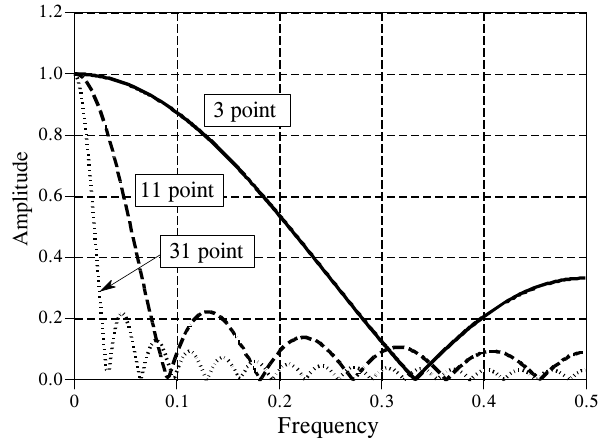
\includegraphics[width=0.507\linewidth,height=0.8\textheight,keepaspectratio]{assets/ch15/fig15-02.png}
\caption*{\textbf{图 15-2　移动平均滤波器的频率响应。}
由于滚降慢、阻带衰减差，移动平均是一个很差的低通滤波器。这些曲线由公式
15-2 生成。 （3 point / 11 point / 31 point = 3 点 / 11 点 / 31
点。Amplitude = 幅度，Frequency = 频率。）}
\end{figure}

\section{移动平均滤波器的亲戚}

在理想世界里，滤波器设计者只需要处理时域编码或频域编码的信息，同一个信号里永远不会两者混杂。可惜，有些应用两个域同时都重要。例如，电视信号就属于这个讨厌的类别。视频信息是在时域编码的，即波形的形状对应图像的亮度分布。然而在传输过程中，视频信号又要按它的频率组成来处理，比如总带宽、伴音和彩色载波怎样加入、直流分量的去除与恢复等。再举一个例子，电磁干扰最好在频域里理解，即使信号的信息是在时域编码的。例如，科学实验中的温度监测信号可能被电源线的
60 Hz、开关电源的 30 kHz 或者本地 AM 电台的 1320 kHz
干扰。移动平均滤波器的亲戚们在频域表现更好，在这类混合域应用中可能很有用。

多次移动平均滤波器(multiple-pass moving average
filter)让输入信号两次或更多次通过移动平均滤波器。图 15-3a
给出了通过一次、两次和四次后得到的总滤波器核。两次相当于使用三角形滤波器核（矩形滤波器核与自身卷积）。四次或更多次之后，等效滤波器核看起来就像高斯曲线（回想中心极限定理）。如
(b) 所示，与一次通过的直线相比，多次通过产生 ``S'' 形的阶跃响应。(c) 和
(d) 中的频率响应等于公式 15-2
自乘通过的次数。也就是说，时域中的每一次卷积，都对应频谱的一次相乘。

\begin{figure}[htbp]
\centering
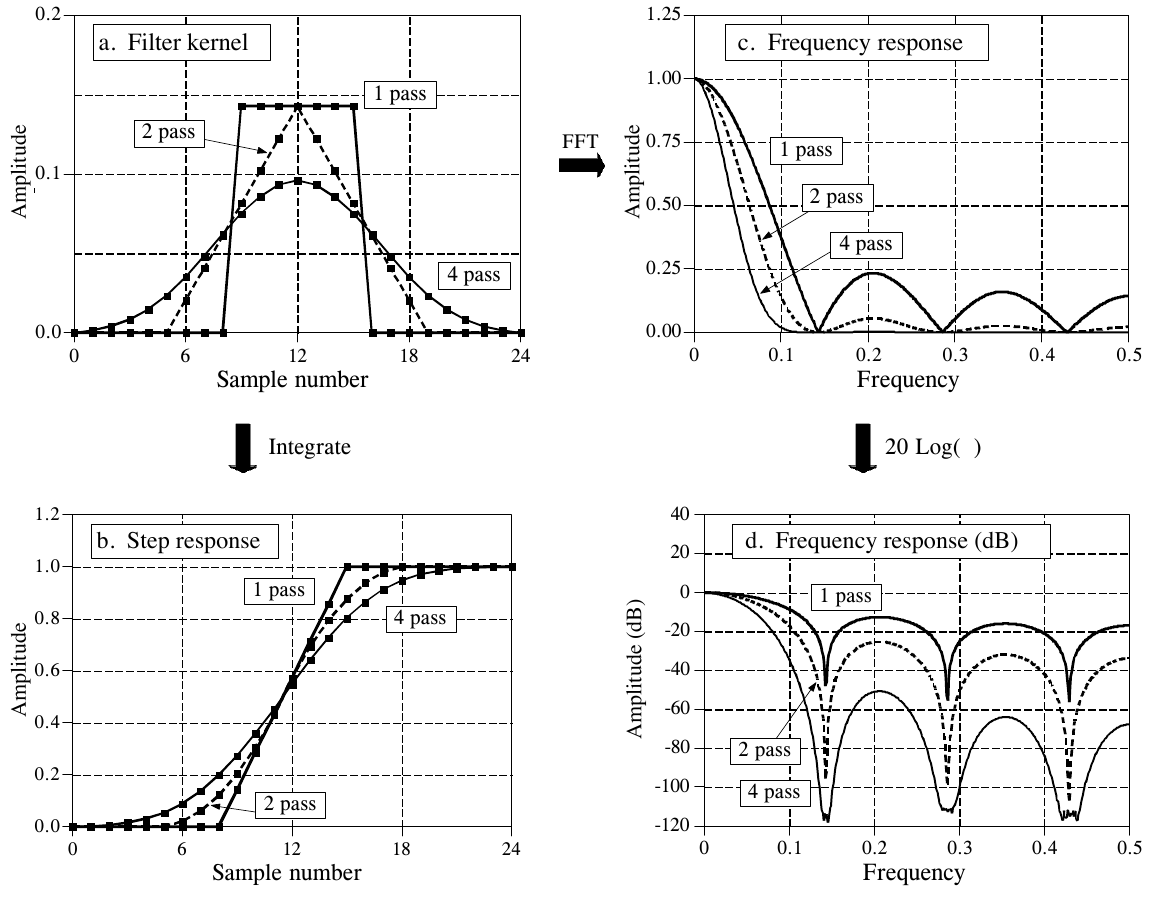
\includegraphics[width=0.963\linewidth,height=0.8\textheight,keepaspectratio]{assets/ch15/fig15-03.png}
\caption*{\textbf{图 15-3　多次移动平均滤波器的特性。} (a) 是让 7
点移动平均滤波器对数据作用一次、两次和四次所得的滤波器核。(b)
是对应的阶跃响应，(c) 和 (d) 是对应的频率响应。 （a. Filter kernel =
滤波器核；b. Step response = 阶跃响应；c.~Frequency response =
频率响应；d.~Frequency response (dB) = 频率响应（分贝）。1 pass / 2 pass
/ 4 pass = 一次 / 两次 / 四次；FFT 箭头表示 (a) 经 FFT 得 (c)；Integrate
= 积分，表示 (a) 经累加得 (b)；20 Log( ) 表示 (c) 取 20 lg 得
(d)。Amplitude = 幅度，Sample number = 采样序号，Frequency = 频率。）}
\end{figure}

图 15-4 是移动平均滤波器另外两个亲戚的频率响应。如第 11
章所讲，用纯高斯曲线作滤波器核时，频率响应也是高斯曲线。高斯曲线很重要，因为它是许多自然和人造系统的冲激响应。例如，一个短促的光脉冲进入一条很长的光纤传输线，由于光子在光纤内走的路径各不相同，出来时会变成一个高斯脉冲。高斯滤波器核在图像处理中也用得很广，因为它有一些独特的性质，能实现快速的二维卷积（见第
24 章）。图 15-4 中的第二条频率响应，对应用布莱克曼窗(Blackman
window)作滤波器核。（这里''窗''一词没有任何含义，只是这条曲线公认名称的一部分。）布莱克曼窗的确切形状在第
16 章给出（公式 16-2、图 16-2），不过它看起来很像高斯曲线。

\begin{figure}[htbp]
\centering
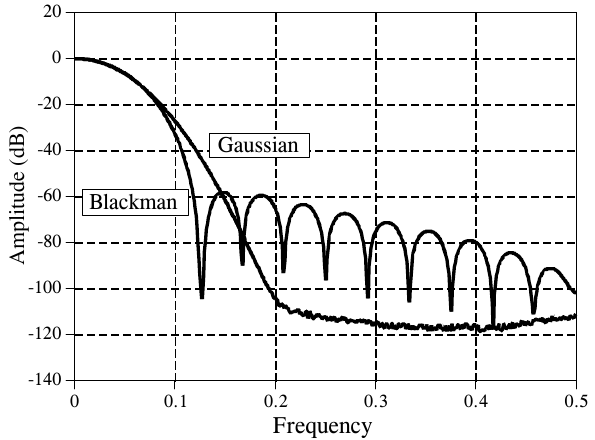
\includegraphics[width=0.496\linewidth,height=0.8\textheight,keepaspectratio]{assets/ch15/fig15-04.png}
\caption*{\textbf{图 15-4　布莱克曼窗和高斯滤波器核的频率响应。}
这两种滤波器的阻带衰减都比移动平均滤波器好。这对去除时域编码信号中的随机噪声没有好处，但在混合域问题中可能有用。这两种滤波器的缺点是必须用卷积，而卷积是一种极慢的算法。
（Gaussian = 高斯，Blackman = 布莱克曼。Amplitude (dB) =
幅度（分贝），Frequency = 频率。）}
\end{figure}

这些移动平均滤波器的亲戚比移动平均本身好在哪里？有三点。第一，也是最重要的一点，它们的阻带衰减比移动平均滤波器好。第二，滤波器核在两端逐渐收窄到较小的幅度。回想一下，输出信号的每个点都是输入中一组采样的加权和。如果滤波器核逐渐收窄，输入信号中离得较远的采样得到的权重就比离得近的小。第三，阶跃响应是平滑的曲线，而不是移动平均那种生硬的直线。后两点通常益处有限，不过你也可能遇到它们确实成为优势的应用。

在保持阶跃响应陡峭的同时降低随机噪声方面，移动平均滤波器和它的亲戚们差不多一样好。分歧在于阶跃响应的上升时间(risetime)怎么量。如果上升时间从阶跃的
0\% 量到
100\%，那么如前所示，移动平均滤波器是你能做到的最好结果。相比之下，如果从
10\% 量到
90\%，布莱克曼窗就比移动平均滤波器好。重点是，这只是理论上的争论；在这个指标上，把这些滤波器看作相同即可。

这些滤波器最大的区别在于执行速度。用递归算法（下面介绍），移动平均滤波器在你的计算机上会快如闪电。事实上，它是现有最快的数字滤波器。多次移动平均会相应地慢一些，但仍然很快。相比之下，高斯和布莱克曼滤波器慢得令人难以忍受，因为它们必须用卷积。可以按''滤波器核点数的十倍''来估计（依据是乘法大约比加法慢
10 倍）。例如，100 点的高斯滤波器预计比用递归实现的移动平均慢 1000 倍。

\section{递归实现}

移动平均滤波器的一大优势是，它可以用一种非常快的算法来实现。要理解这个算法，设想让输入信号
x{[} {]} 通过一个 7 点移动平均滤波器，得到输出信号 y{[}
{]}。看看相邻两个输出点 y{[}50{]} 和 y{[}51{]} 是怎么算的：

\[y[50] = x[47] + x[48] + x[49] + x[50] + x[51] + x[52] + x[53]\]

\[y[51] = x[48] + x[49] + x[50] + x[51] + x[52] + x[53] + x[54]\]

这两个计算几乎相同：x{[}48{]} 到 x{[}53{]} 这几个点算 y{[}50{]}
时要加一遍，算 y{[}51{]} 时还要再加一遍。如果 y{[}50{]}
已经算出来了，计算 y{[}51{]} 最高效的办法是：

\[y[51] = y[50] + x[54] - x[47]\]

用 y{[}50{]} 求出 y{[}51{]} 之后，就可以由 y{[}51{]} 算出
y{[}52{]}，依此类推。算出 y{[} {]}
的第一个点之后，其余每个点都只需要一次加法和一次减法。这可以写成公式：

\textbf{公式 15-3}　移动平均滤波器的递归实现。式中 x{[} {]}
是输入信号，y{[} {]} 是输出信号，M
是移动平均的点数（奇数）。使用这个公式之前，信号的第一个点必须用普通求和算出。

\[y[i] = y[i-1] + x[i+p] - x[i-q], \qquad p = (M-1)/2, \quad q = p + 1\]

\begin{quote}
\textbf{译注：} 上面 y{[}50{]}、y{[}51{]} 的两个式子是 7
个点的和，原书为了简洁省略了除以 7；公式 15-3 同样省略了
1/M。照字面算，y 是窗口内的和而不是平均，实际使用时要再除以
M（或者在加减时就用 x/M）。
\end{quote}

注意这个公式用两种数据来源计算输出中的每个点：输入中的点，以及输出中先前算好的点。这叫做递归方程(recursive
equation)，意思是一次计算的结果会用于以后的计算。（``递归''一词也有别的含义，尤其在计算机科学中。）第
19
章会更详细地讨论各种递归滤波器。要注意，移动平均递归滤波器与典型的递归滤波器很不一样。特别是，大多数递归滤波器的冲激响应无限长（无限冲激响应，infinite
impulse
response，IIR），由正弦和指数组成。而移动平均的冲激响应是一个矩形脉冲（有限冲激响应，finite
impulse response，FIR）。

这个算法比其他数字滤波器快，原因有几个。第一，无论滤波器核多长，每个点都只有两次运算。第二，只需要加法和减法，而大多数数字滤波器需要耗时的乘法。第三，索引方式非常简单。公式
15-3 中的每个下标，都是加上或减去一个在滤波开始前就能算好的整数常数（即
p 和
q）。第四，整个算法可以全部用整数表示来完成。根据所用的硬件，整数运算可能比浮点运算快一个数量级以上。

\begin{quote}
\textbf{译注：} 原书把 ``Fourth'' 拼成了 ``Forth''。
\end{quote}

出人意料的是，对这个算法而言，整数表示不但更快，效果也比浮点更好。如果不小心，浮点运算的舍入误差(round-off
error)会造成意想不到的结果。例如，设想用这种方法处理一个 10,000
个采样的信号。滤波后信号的最后一个采样，带有 10,000 次加法和 10,000
次减法累积下来的误差。这在输出信号中表现为一个漂移的偏移量。整数没有这个问题，因为整数运算没有舍入误差。如果你必须在这个算法中用浮点数，表
15-2 的程序展示了怎样用双精度累加器来消除这种漂移。

\textbf{表 15-2}（注释已译成中文）

\begin{Shaded}
\begin{Highlighting}[]
\NormalTok{100 \textquotesingle{}MOVING AVERAGE FILTER IMPLEMENTED BY RECURSION}
\NormalTok{110 \textquotesingle{}这个程序用 101 点移动平均滤波器处理 5000 个采样，}
\NormalTok{120 \textquotesingle{}得到 4900 个滤波后的数据。}
\NormalTok{130 \textquotesingle{}使用双精度累加器，防止舍入造成的漂移。}
\NormalTok{140 \textquotesingle{}}
\NormalTok{150 DIM X[4999]                        \textquotesingle{}X[ ] 存放输入信号}
\NormalTok{160 DIM Y[4999]                        \textquotesingle{}Y[ ] 存放输出信号}
\NormalTok{170 DEFDBL ACC                         \textquotesingle{}把变量 ACC 定义为双精度}
\NormalTok{180 \textquotesingle{}}
\NormalTok{190 GOSUB XXXX                         \textquotesingle{}虚构的子程序，载入 X[ ]}
\NormalTok{200 \textquotesingle{}}
\NormalTok{210 ACC = 0                            \textquotesingle{}把 X[0] 到 X[100] 平均，求出 Y[50]}
\NormalTok{220 FOR I\% = 0 TO 100}
\NormalTok{230 ACC = ACC + X[I\%]}
\NormalTok{240 NEXT I\%}
\NormalTok{250 Y[[50] = ACC/101}
\NormalTok{260 \textquotesingle{}                                  \textquotesingle{}递归移动平均滤波器（公式 15{-}3）}
\NormalTok{270 FOR I\% = 51 TO 4949}
\NormalTok{280 ACC = ACC + X[I\%+50] {-} X[I\%{-}51]}
\NormalTok{290 Y[I\%] = ACC}
\NormalTok{300 NEXT I\%}
\NormalTok{310 \textquotesingle{}}
\NormalTok{320 END}
\end{Highlighting}
\end{Shaded}

\begin{quote}
\textbf{译注：} 第 250 行 \texttt{Y{[}{[}50{]}} 多了一个左括号，应为
\texttt{Y{[}50{]}}。第 290 行原书写成
\texttt{Y{[}I\%{]}\ =\ ACC}，漏了除以 101：ACC 是 101 个点的和，第 250
行算 Y{[}50{]} 时除了 101，这里也应写成
\texttt{Y{[}I\%{]}\ =\ ACC/101}，否则从第 51 点起输出会突然变成 101 倍。
\end{quote}

\textbf{C 实现}（完整可编译版本见
\texttt{c/table15-2\_recursive\_moving\_average.c}，信号与表 15-1 的 C
版本相同；程序还附带一个单精度累加器的版本，用来复现书里说的舍入漂移）：

\begin{Shaded}
\begin{Highlighting}[]
\PreprocessorTok{\#define HALF }\DecValTok{50}\PreprocessorTok{                             }\CommentTok{/* p = 50，q = 51 */}
\PreprocessorTok{\#define M    }\OperatorTok{(}\DecValTok{2}\PreprocessorTok{ }\OperatorTok{*}\PreprocessorTok{ HALF }\OperatorTok{+}\PreprocessorTok{ }\DecValTok{1}\OperatorTok{)}\PreprocessorTok{                 }\CommentTok{/* 101 点 */}

\CommentTok{/* 表 15{-}2：递归实现，累加器 ACC 用 double（第 170 行 DEFDBL ACC） */}
\DataTypeTok{static} \DataTypeTok{void}\NormalTok{ recursive\_double}\OperatorTok{(}\DataTypeTok{const} \DataTypeTok{float} \OperatorTok{*}\NormalTok{x}\OperatorTok{,} \DataTypeTok{float} \OperatorTok{*}\NormalTok{y}\OperatorTok{,} \DataTypeTok{int}\NormalTok{ n}\OperatorTok{)}
\OperatorTok{\{}
    \DataTypeTok{double}\NormalTok{ acc }\OperatorTok{=} \FloatTok{0.0}\OperatorTok{;}                       \CommentTok{/* 210：ACC = 0 */}
    \ControlFlowTok{for} \OperatorTok{(}\DataTypeTok{int}\NormalTok{ i }\OperatorTok{=} \DecValTok{0}\OperatorTok{;}\NormalTok{ i }\OperatorTok{\textless{}=} \DecValTok{2} \OperatorTok{*}\NormalTok{ HALF}\OperatorTok{;}\NormalTok{ i}\OperatorTok{++)}     \CommentTok{/* 220～240：先把 X[0]～X[100] 加起来 */}
\NormalTok{        acc }\OperatorTok{+=}\NormalTok{ x}\OperatorTok{[}\NormalTok{i}\OperatorTok{];}
\NormalTok{    y}\OperatorTok{[}\NormalTok{HALF}\OperatorTok{]} \OperatorTok{=} \OperatorTok{(}\DataTypeTok{float}\OperatorTok{)(}\NormalTok{acc }\OperatorTok{/}\NormalTok{ M}\OperatorTok{);}             \CommentTok{/* 250：Y[50] = ACC/101 */}
    \ControlFlowTok{for} \OperatorTok{(}\DataTypeTok{int}\NormalTok{ i }\OperatorTok{=}\NormalTok{ HALF }\OperatorTok{+} \DecValTok{1}\OperatorTok{;}\NormalTok{ i }\OperatorTok{\textless{}}\NormalTok{ n }\OperatorTok{{-}}\NormalTok{ HALF}\OperatorTok{;}\NormalTok{ i}\OperatorTok{++)} \OperatorTok{\{} \CommentTok{/* 270：FOR I\% = 51 TO 4949 */}
\NormalTok{        acc }\OperatorTok{+=}\NormalTok{ x}\OperatorTok{[}\NormalTok{i }\OperatorTok{+}\NormalTok{ HALF}\OperatorTok{]} \OperatorTok{{-}}\NormalTok{ x}\OperatorTok{[}\NormalTok{i }\OperatorTok{{-}}\NormalTok{ HALF }\OperatorTok{{-}} \DecValTok{1}\OperatorTok{];}   \CommentTok{/* 280：加上新进窗口的点，减去刚出窗口的点 */}
\NormalTok{        y}\OperatorTok{[}\NormalTok{i}\OperatorTok{]} \OperatorTok{=} \OperatorTok{(}\DataTypeTok{float}\OperatorTok{)(}\NormalTok{acc }\OperatorTok{/}\NormalTok{ M}\OperatorTok{);}            \CommentTok{/* 290：原书漏了 /101，这里补上 */}
    \OperatorTok{\}}
\OperatorTok{\}}
\end{Highlighting}
\end{Shaded}

运行结果（与直接求和逐点比较）：

{\def\LTcaptype{none} % do not increment counter
\begin{longtable}[]{@{}llll@{}}
\toprule\noalign{}
信号 & 累加器 & 最大偏差 & 最后一点偏差 \\
\midrule\noalign{}
\endhead
\bottomrule\noalign{}
\endlastfoot
5000 点（原书设定） & double & 7.5e-8 & 1.4e-8 \\
5000 点（原书设定） & float & 5.6e-7 & 1.1e-7 \\
100 万点，带 100 的直流偏置 & double & 3.8e-6 & 3.3e-6 \\
100 万点，带 100 的直流偏置 & float & 0.0056 & 0.0041 \\
\end{longtable}
}

5000
点时两种累加器都和直接求和一致（偏差在单精度输出的舍入量级）。信号一长、数值一大，float
累加器的误差就逐点累积，最大偏差比 double 大约 1500
倍，这就是书中说的''漂移的偏移量''。double 那一行的 3.8e-6 只是输出存成
float 时的舍入（100 附近 float 的分辨率约 7.6e-6），不是漂移。

% !TEX root = ../main.tex
% 本文件由 build-tex.sh 从 16-DSP指南-第16章中译.md 生成，改内容请改 md 后重新生成

\chapter{加窗 sinc 滤波器}\label{ch-16}

加窗 sinc 滤波器(windowed-sinc
filter)用来把一个频带与另一个频带分开。它们非常稳定，很少出意外，而且性能可以推到惊人的高度。这些出色的频域特性，是以时域表现很差为代价换来的，包括阶跃响应中过大的振铃(ripple)和过冲(overshoot)。用标准卷积实现时，加窗
sinc 滤波器很容易编程，但执行很慢。第 18 章会说明怎样用 FFT
大幅提高这类滤波器的计算速度。

\section{加窗 sinc 的思路}

图 16-1 说明了加窗 sinc 滤波器背后的想法。(a)
是理想低通滤波器的频率响应：低于截止频率 \(f_C\) 的所有频率都以幅度 1
通过，高于它的所有频率都被挡住。通带(passband)完全平坦，阻带(stopband)的衰减无穷大，两者之间的过渡无限窄。

对这个理想频率响应做逆傅里叶变换，就得到 (b)
所示的理想滤波器核（冲激响应）。前面讨论过（见第 11 章公式
11-4），这条曲线的一般形式是 \(\sin(x)/x\)，叫做 sinc 函数，表达式为：

\[h[i] = \frac{\sin(2\pi f_C\, i)}{i\pi}\]

把输入信号与这个滤波器核卷积，就是一个完美的低通滤波器。问题在于，sinc
函数一直延伸到负无穷和正无穷，幅度不会降到零。这种无限长度对数学不成问题，对计算机却是致命的。

为了绕开这个问题，我们对 (b) 中的 sinc 函数做两处修改，得到 (c)
所示的波形。第一，把它截断成 M+1 个点，围绕主瓣(main
lobe)对称地选取，其中 M 是偶数。这 M+1
个点以外的所有采样都设为零，或者干脆不管。第二，把整个序列向右平移，让它从
0 跑到
M。这样滤波器核只用正下标就能表示。虽然很多编程语言允许负下标，但用起来很麻烦。滤波器核平移
M/2 的唯一影响，是输出信号也平移同样的量。

由于修改后的滤波器核只是理想滤波器核的近似，它的频率响应不会是理想的。要知道实际得到的频率响应，可以对
(c) 中的信号做傅里叶变换，得到 (d)
中的曲线。一团糟！通带里有过大的波纹，阻带衰减很差（回想第 11
章讨论的吉布斯效应(Gibbs effect)）。这些问题源于截断后的 sinc
函数两端的突然间断。增加滤波器核的长度并不能减轻这些问题：不管 M
取多大，这个间断都很显著。

幸好有一个简单的办法能改善这种状况。(e)
是一条平滑渐收的曲线，叫做布莱克曼窗(Blackman window)。把截断的 sinc (c)
乘以布莱克曼窗 (e)，得到 (f) 所示的加窗 sinc
滤波器核。目的是让截断处不那么突兀，从而改善频率响应。(g)
显示了这一改善：通带现在是平的，阻带衰减好到在这张图上都看不出来。

可用的窗(window)有好几种，大多以 1950
年代最早提出它们的人命名。值得用的只有两种：汉明窗(Hamming
window)和布莱克曼窗。它们的表达式是：

\textbf{公式 16-1}　汉明窗。这些窗的 i 从 0 跑到 M，共 M+1 个点。

\[w[i] = 0.54 - 0.46\cos(2\pi i/M)\]

\textbf{公式 16-2}　布莱克曼窗。

\[w[i] = 0.42 - 0.5\cos(2\pi i/M) + 0.08\cos(4\pi i/M)\]

\begin{figure}[htbp]
\centering
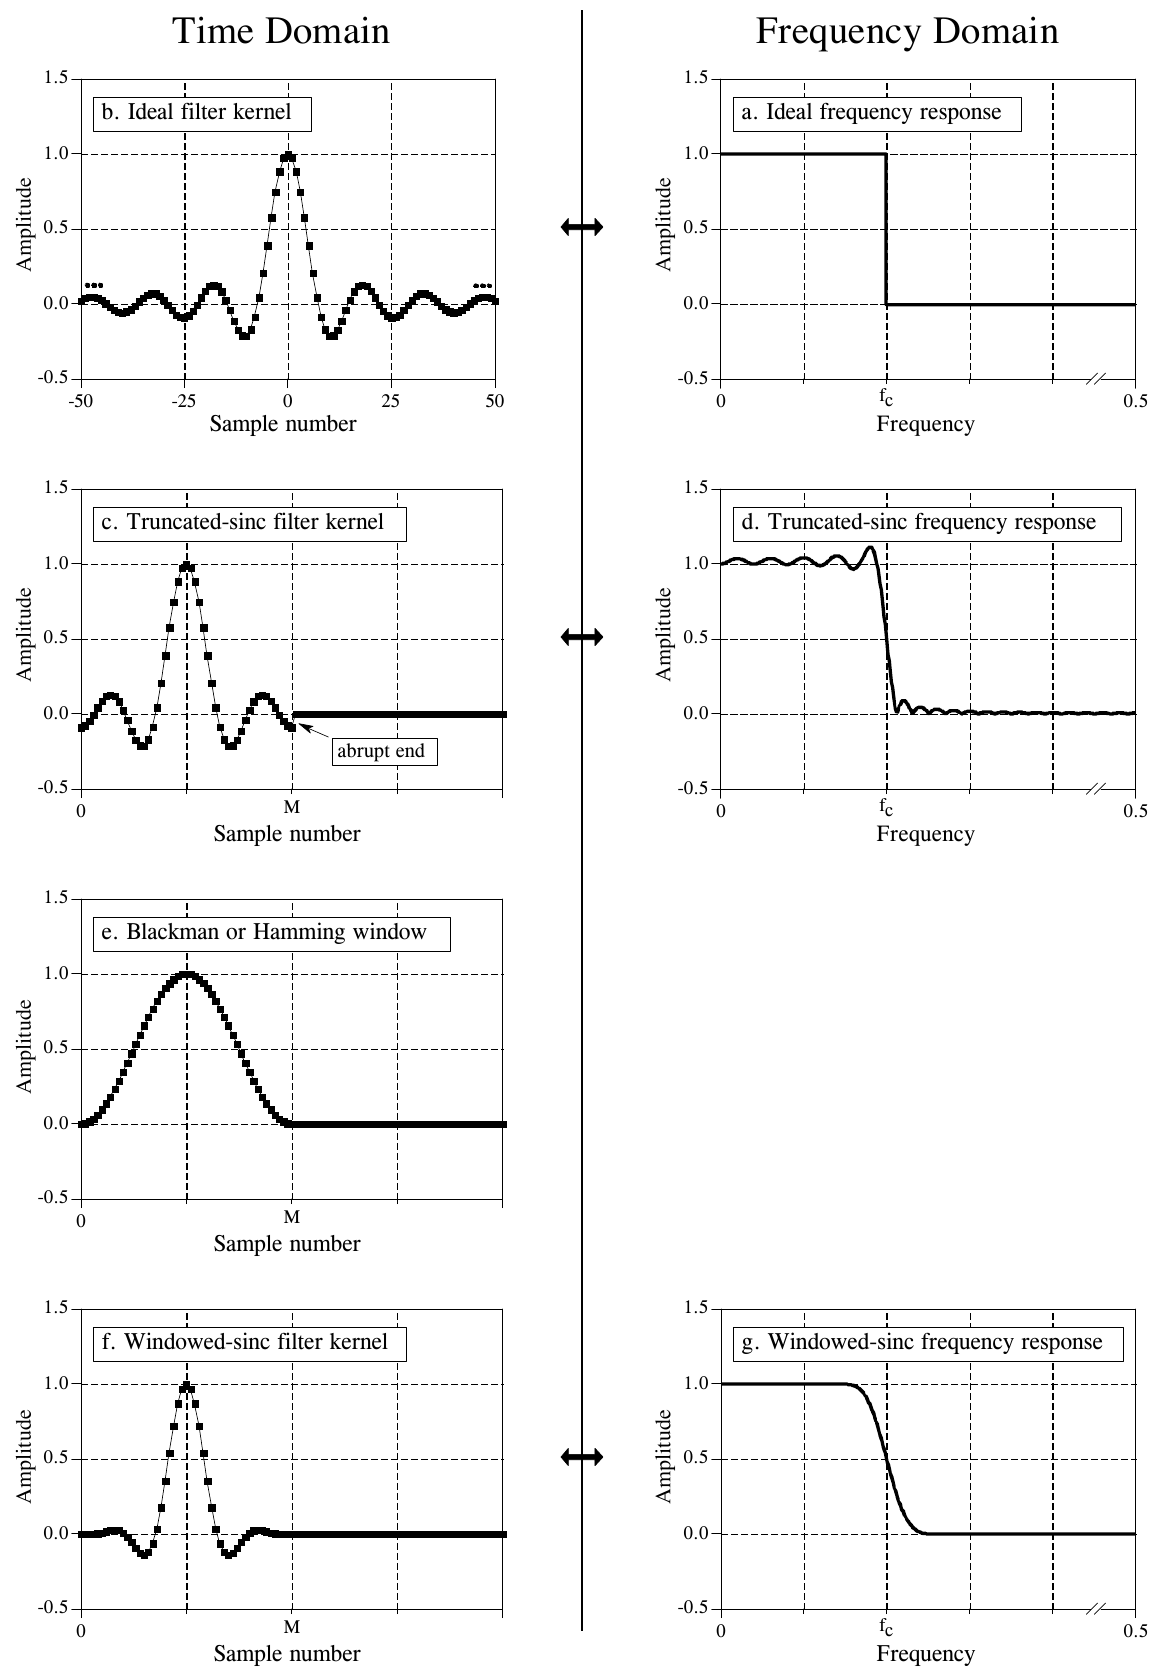
\includegraphics[width=0.958\linewidth,height=0.8\textheight,keepaspectratio]{assets/ch16/fig16-01.png}
\caption*{\textbf{图 16-1　加窗 sinc 滤波器核的推导。} (a)
是理想低通滤波器的频率响应，(b) 是对应的滤波器核，即 sinc 函数。由于
sinc 无限长，要在计算机里使用就必须截断，如 (c)
所示。然而，截断给频率响应带来了不希望有的变化 (d)。解决办法是把截断的
sinc 乘以一个平滑的窗 (e)，得到加窗 sinc 滤波器核 (f)。加窗 sinc
的频率响应 (g) 平滑而规矩。这些图没有按比例绘制。 （Time Domain =
时域，Frequency Domain = 频域；a. Ideal frequency response =
理想频率响应，b. Ideal filter kernel = 理想滤波器核，c.~Truncated-sinc
filter kernel = 截断 sinc 滤波器核，d.~Truncated-sinc frequency response
= 截断 sinc 的频率响应，e. Blackman or Hamming window =
布莱克曼窗或汉明窗，f.~Windowed-sinc filter kernel = 加窗 sinc
滤波器核，g. Windowed-sinc frequency response = 加窗 sinc
的频率响应；abrupt end = 突然截断的端点。Amplitude = 幅度，Sample number
= 采样序号，Frequency = 频率。原书这张图排在单独一页，图注写作 ``facing
page''（见对页）。）}
\end{figure}

图 16-2a 画出了 M = 50（即曲线共 51
个点）时这两种窗的形状。该用哪一种？这是参数之间的权衡。如图 16-2b
所示，汉明窗的滚降(roll-off)比布莱克曼窗快约 20\%。然而，(c)
表明布莱克曼窗的阻带衰减更好。确切地说，布莱克曼窗的阻带衰减是 −74
dB（约 0.02\%），而汉明窗只有 −53 dB（约
0.2\%）。虽然在这些图里看不出来，布莱克曼窗的通带波纹只有约
0.02\%，而汉明窗一般是
0.2\%。总的来说，布莱克曼窗应当是你的首选：滚降慢一点比阻带衰减差更容易应付。

\begin{figure}[htbp]
\centering
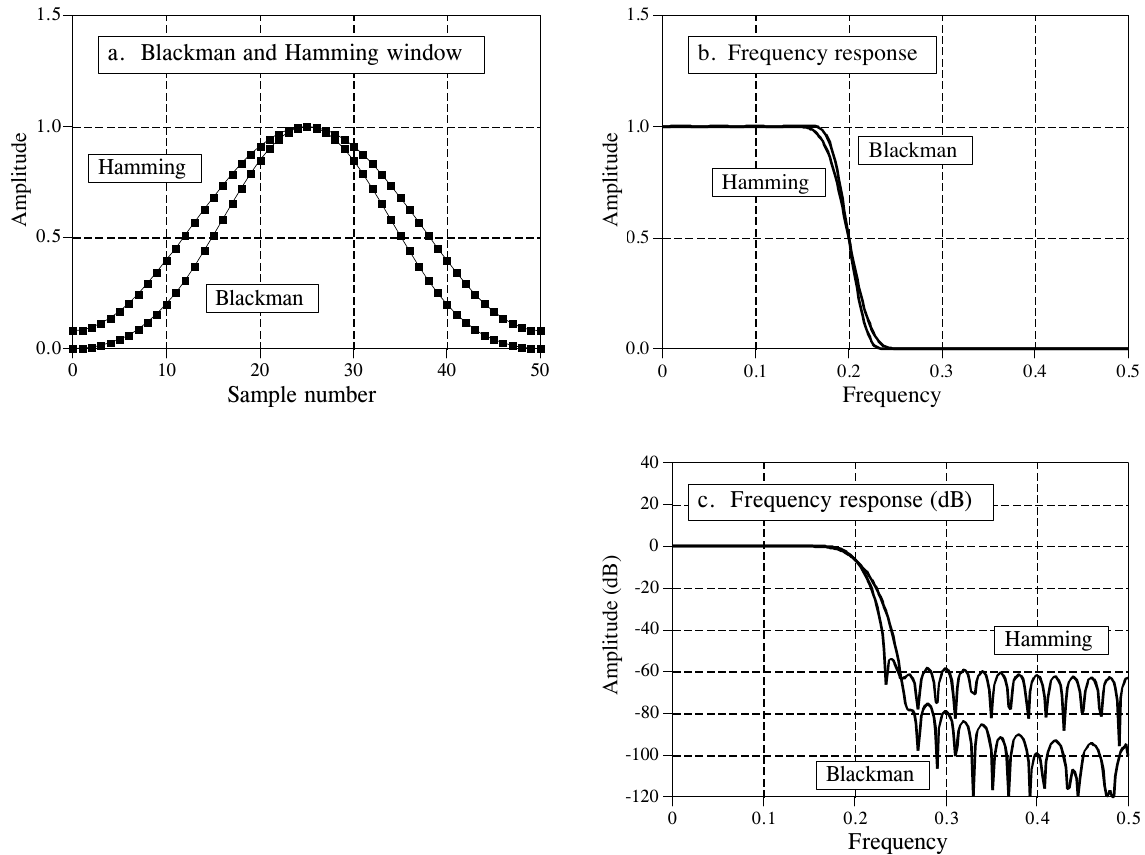
\includegraphics[width=0.954\linewidth,height=0.8\textheight,keepaspectratio]{assets/ch16/fig16-02.png}
\caption*{\textbf{图 16-2　布莱克曼窗和汉明窗的特性。} (a)
是这两种窗的形状，由公式 16-1 和 16-2 给出。如 (b)
所示，汉明窗的滚降比布莱克曼窗快约
20\%。然而，布莱克曼窗的阻带衰减更好（布莱克曼：0.02\%，汉明：0.2\%），通带波纹也更低（布莱克曼：0.02\%，汉明：0.2\%）。
（a. Blackman and Hamming window = 布莱克曼窗与汉明窗，b. Frequency
response = 频率响应，c.~Frequency response (dB) =
频率响应（分贝）；Hamming = 汉明，Blackman = 布莱克曼。Amplitude =
幅度，Amplitude (dB) = 幅度（分贝），Sample number = 采样序号，Frequency
= 频率。原书英文图注排在 (c) 左侧，裁图时已擦掉，译文见上。）}
\end{figure}

你可能还会听说别的窗，不过它们都比不上布莱克曼窗和汉明窗。巴特利特窗(Bartlett
window)是一个三角形，用直线做渐收。汉宁窗(Hanning
window)也叫升余弦窗(raised cosine window)，表达式是
\(w[i] = 0.5 - 0.5\cos(2\pi i/M)\)。这两种窗的滚降速度和汉明窗差不多，但阻带衰减更差（巴特利特：−25
dB，即 5.6\%；汉宁：−44 dB，即 0.63\%）。你也可能听说矩形窗(rectangular
window)。它等于不加窗，只是把尾部截掉（就像图 16-1c
那样）。它的滚降比布莱克曼窗快约 2.5 倍，但阻带衰减只有 −21
dB（8.9\%）。

\section{设计滤波器}

设计一个加窗 sinc 滤波器要选两个参数：截止频率 \(f_C\) 和滤波器核的长度
M。截止频率用采样率的分数表示，因此必须在 0 到 0.5 之间。M
的取值按下面的近似式决定滚降：

\textbf{公式 16-3}　滤波器长度与滚降的关系。滤波器核的长度 M
决定滤波器的过渡带宽 BW。这只是一个近似，因为滚降还取决于所用的窗。

\[M \approx \frac{4}{BW}\]

其中 BW 是过渡带(transition band)的宽度，从曲线刚刚离开 1
的地方量到它几乎降到 0 的地方（比如曲线的 99\% 到
1\%）。过渡带宽也用采样频率的分数表示，必须在 0 到 0.5 之间。图 16-3a
是使用这个近似式的一个例子。图中三条曲线由 M = 20、40 和 200
的滤波器核得到。由公式 16-3，过渡带宽分别是 BW = 0.2、0.1 和 0.02。(b)
表明频率响应的形状不随所选的截止频率变化。

\begin{figure}[htbp]
\centering
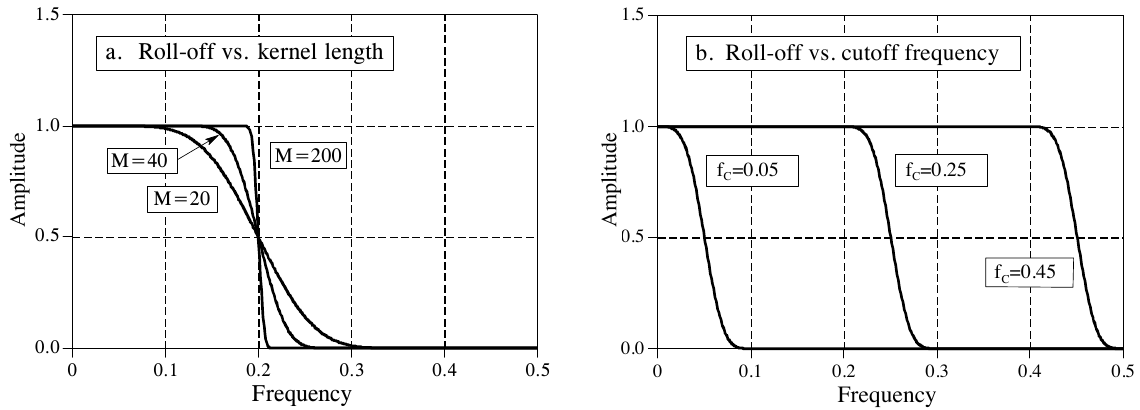
\includegraphics[width=0.950\linewidth,height=0.8\textheight,keepaspectratio]{assets/ch16/fig16-03.png}
\caption*{\textbf{图 16-3　加窗 sinc 滤波器的长度与滚降。} 如 (a) 所示，M = 20、40
和 200 时，过渡带宽分别是采样率的 BW = 0.2、0.1 和 0.02。如 (b)
所示，截止频率不同时，频率响应的形状不变。(b) 中 M = 60。 （a. Roll-off
vs.~kernel length = 滚降与核长度，b. Roll-off vs.~cutoff frequency =
滚降与截止频率。Amplitude = 幅度，Frequency = 频率。）}
\end{figure}

由于卷积所需的时间与信号长度成正比，公式 16-3 体现的是计算时间（取决于
M）与滤波器陡峭程度（BW
的值）之间的权衡。例如，布莱克曼窗（与汉明窗相比）慢 20\%
的滚降，可以用长 20\%
的滤波器核来弥补。换句话说，可以说布莱克曼窗比滚降相当的汉明窗执行起来慢
20\%。这一点很重要，因为加窗 sinc 滤波器的执行速度本来就慢得要命。

同样如图 16-3b 所示，加窗 sinc
滤波器的截止频率是在幅度一半的地方测量的。为什么用
0.5，而不用模拟电子学和其他数字滤波器中标准的 0.707（−3
dB）？这是因为加窗 sinc
的频率响应在通带和阻带之间是对称的。例如，汉明窗的通带波纹是
0.2\%，阻带衰减（即阻带中的波纹）也同样是
0.2\%。其他滤波器没有这种对称性，因此用半幅点标记截止频率对它们没有好处。本章后面会看到，这种对称性使加窗
sinc 非常适合做频谱反转(spectral inversion)。

选好 \(f_C\) 和 M 之后，滤波器核按下式计算：

\textbf{公式 16-4}　加窗 sinc 滤波器核。截止频率 \(f_C\)
用采样率的分数表示，取值在 0 到 0.5 之间。滤波器核的长度由 M 决定，M
必须是偶数。采样序号 i 是从 0 到 M 的整数，滤波器核共 M+1 个点。常数 K
的选取使零频率处的增益为 1。为避免除零错误，在 i = M/2 处取
\(h[i] = 2\pi f_C K\)。

\[h[i] = K\,\frac{\sin\!\big(2\pi f_C\,(i - M/2)\big)}{i - M/2}\left[0.42 - 0.5\cos\!\left(\frac{2\pi i}{M}\right) + 0.08\cos\!\left(\frac{4\pi i}{M}\right)\right]\]

别被这个式子吓住！根据前面的讨论，你应该能认出其中的三个部分：sinc
函数、M/2 的平移和布莱克曼窗。要让滤波器在直流处的增益为 1，常数 K
必须选得使所有采样之和等于 1。实际做法是：算滤波器核时先不管
K，算完再把所有采样按需要归一化。表 16-1 的程序展示了怎样做。还要注意
sinc 中心 i = M/2 处的计算是怎么处理的，那里会出现除以零。

这个式子虽然长，用起来却很简单：把它敲进程序就可以不管了，让计算机去算。如果你发现自己在手算这个式子，那你一定是做错了什么。

具体说一下公式 16-4
描述的滤波器核在计算机数组里放在什么位置。举个例子，取 M = 100。记住，M
必须是偶数。滤波器核的第一个点在数组位置 0，最后一个点在数组位置
100。这意味着整个信号长 101 个点。对称中心在第 50 点，即 M/2。第 50
点左边的 50 个点与右边的 50 个点对称：第 0 点与第 100 点的值相同，第 49
点与第 51 点相同。如果你一定要让滤波器核有特定数量的采样（比如为了用
FFT），只要在一端或另一端补零即可。例如 M = 100 时，可以把第 101 到 127
个采样设为零，得到一个 128 点长的滤波器核。

\begin{figure}[htbp]
\centering
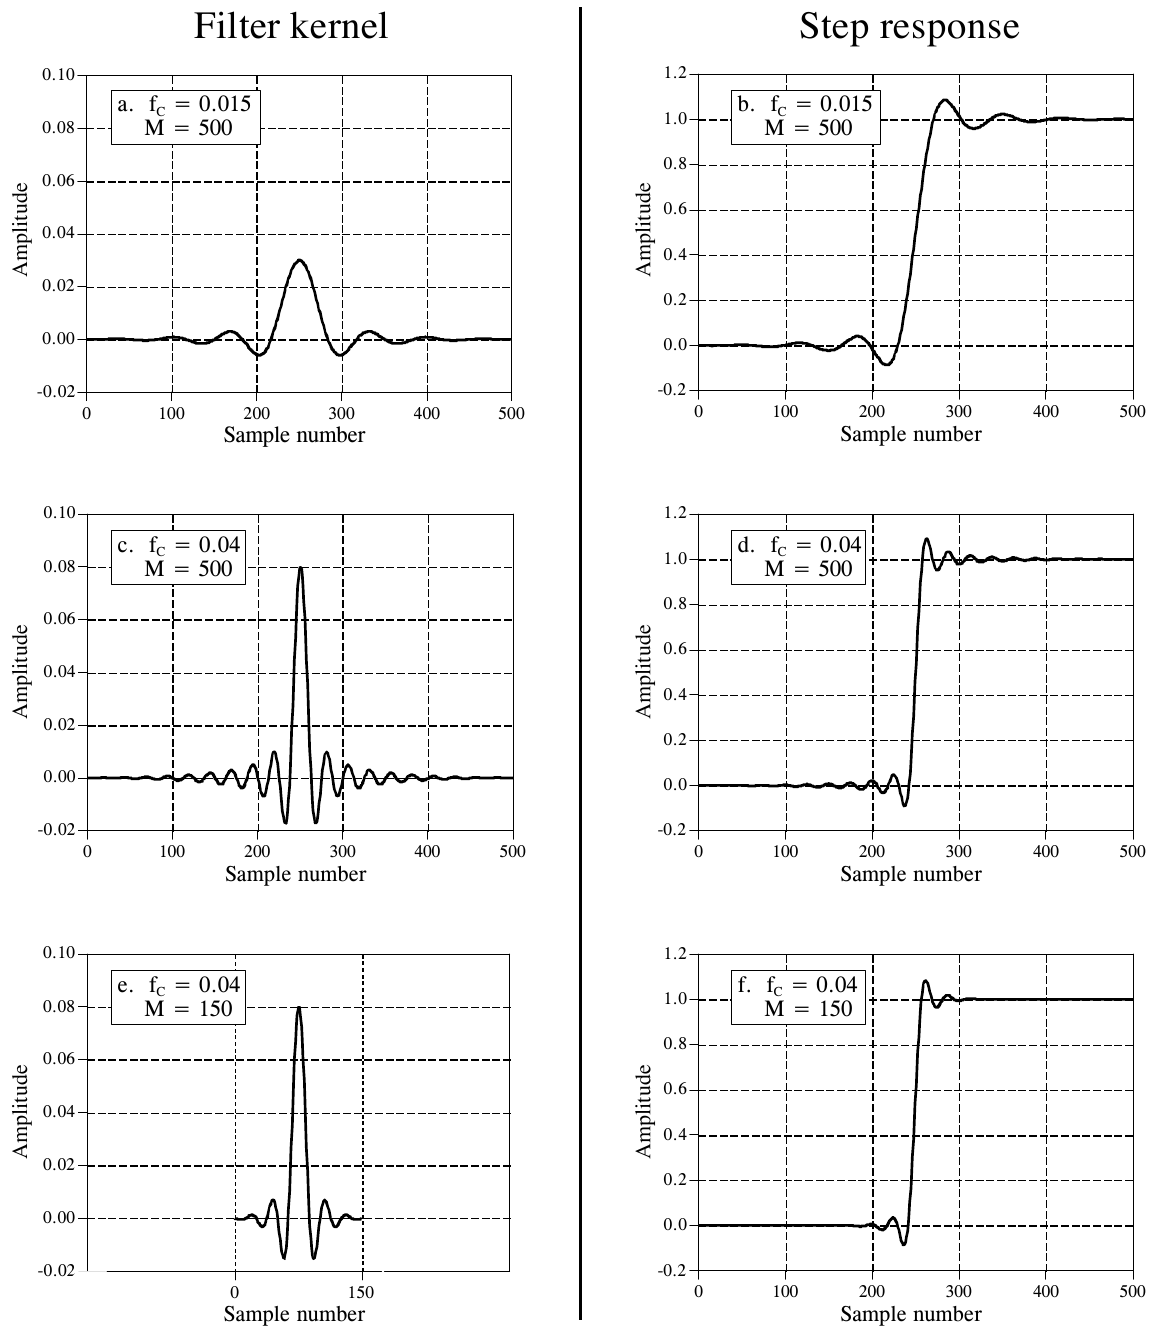
\includegraphics[width=0.958\linewidth,height=0.8\textheight,keepaspectratio]{assets/ch16/fig16-04.png}
\caption*{\textbf{图 16-4　滤波器核示例及对应的阶跃响应。}
正弦振荡的频率大约等于截止频率 \(f_C\)，而 M 决定核的长度。 （Filter
kernel = 滤波器核，Step response = 阶跃响应。Amplitude = 幅度，Sample
number = 采样序号。(e) 的横轴在原书 PDF 中抽取时显示为 ``−175 0
150175''，图上实际只标了 0 和 150。）}
\end{figure}

图 16-4 给出了加窗 sinc 滤波器核的例子，以及它们对应的阶跃响应(step
response)。滤波器核开头和结尾的采样非常小，在图上甚至看不出来。别误以为它们不重要！这些采样的值也许很小，但它们合起来对滤波器的性能有很大影响。这也是加窗
sinc
滤波器通常用浮点数实现的原因：整数通常没有足够的动态范围，装不下滤波器核里大小悬殊的数值。加窗
sinc
滤波器在时域表现如何？很糟糕！阶跃响应有过冲和振铃；对于信息编码在时域里的信号，这不是该用的滤波器。

\section{加窗 sinc 滤波器的例子}

脑电图（electroencephalogram，EEG）是对大脑电活动的测量。它可以通过贴在头皮表面的电极测到，是毫伏级的信号。大脑中的每个神经细胞都会产生微小的电脉冲。EEG
是大量这种电脉冲以（但愿是）协调的方式产生后的综合结果。虽然人们对思维与这种电协调之间的关系知之甚少，但
EEG 中的不同频率可以和特定的精神状态对应起来。如果你闭上眼睛放松，EEG
的主要模式会是一个约 7 到 12 赫兹之间的缓慢振荡。这个波形叫做 α
节律(alpha rhythm)，与满足和注意力下降有关。睁开眼睛四处张望，EEG 会变成
β 节律(beta rhythm)，频率约在 17 到 20
赫兹之间。在儿童身上、不同深度的睡眠中，以及癫痫等各种脑部疾病中，还能看到其他频率和波形。

在这个例子中，我们假设 EEG 信号已经由模拟电路放大，然后以每秒 100
个采样的采样率数字化。采集 50 秒的数据，得到一个 5000
点的信号。我们的目标是把 α 节律和 β
节律分开。为此，我们设计一个截止频率为 14 赫兹（即采样率的
0.14）的数字低通滤波器。过渡带宽定为 4 赫兹，即采样率的 0.04。由公式
16-3，滤波器核需要约 101 个点长，我们随意选用汉明窗。表 16-1
的程序展示了怎样实现这个滤波器。对滤波器核做傅里叶变换得到的频率响应，如图
16-5 所示。

\begin{figure}[htbp]
\centering
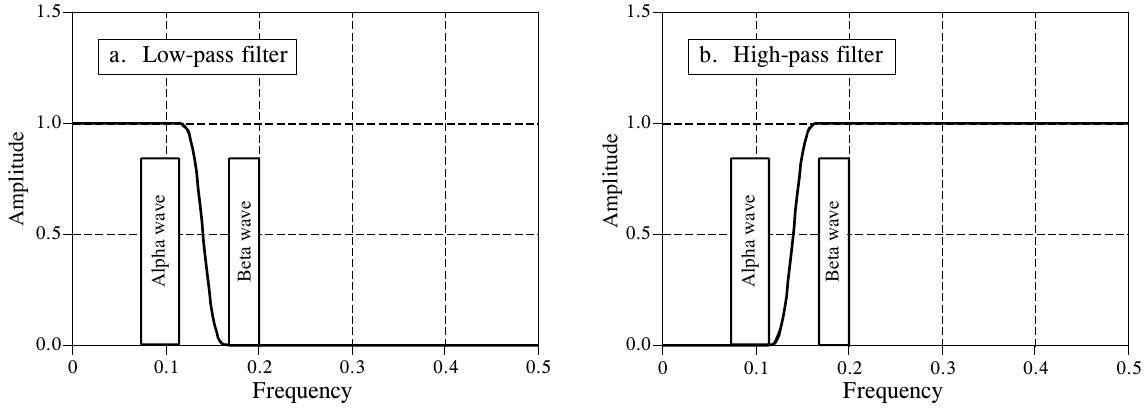
\includegraphics[width=0.954\linewidth,height=0.8\textheight,keepaspectratio]{assets/ch16/fig16-05.png}
\caption*{\textbf{图 16-5　加窗 sinc 滤波器的例子。} 用 M = 100
的低通和高通滤波器把 EEG 中的 α 节律和 β
节律分开。实现低通滤波器的程序见表
16-1。高通滤波器的程序与之相同，只是对低通滤波器核做了频谱反转。 （a.
Low-pass filter = 低通滤波器，b. High-pass filter = 高通滤波器；Alpha
wave = α 波，Beta wave = β 波。Amplitude = 幅度，Frequency = 频率。）}
\end{figure}

\textbf{表 16-1}（注释已译成中文）

\begin{Shaded}
\begin{Highlighting}[]
\NormalTok{100 \textquotesingle{}LOW{-}PASS WINDOWED{-}SINC FILTER}
\NormalTok{110 \textquotesingle{}本程序用 101 点的加窗 sinc 滤波器对 5000 个采样滤波，}
\NormalTok{120 \textquotesingle{}得到 4900 个滤波后的数据。}
\NormalTok{130 \textquotesingle{}}
\NormalTok{140 DIM X[4999]                       \textquotesingle{}X[ ] 存放输入信号}
\NormalTok{150 DIM Y[4999]                       \textquotesingle{}Y[ ] 存放输出信号}
\NormalTok{160 DIM H[100]                        \textquotesingle{}H[ ] 存放滤波器核}
\NormalTok{170 \textquotesingle{}}
\NormalTok{180 PI = 3.14159265}
\NormalTok{190 FC = .14                          \textquotesingle{}设定截止频率（0 到 0.5 之间）}
\NormalTok{200 M\% = 100                          \textquotesingle{}设定滤波器长度（101 点）}
\NormalTok{210 \textquotesingle{}}
\NormalTok{220 GOSUB XXXX                        \textquotesingle{}虚构的子程序，载入 X[ ]}
\NormalTok{230 \textquotesingle{}}
\NormalTok{240 \textquotesingle{}                                 \textquotesingle{}按公式 16{-}4 计算低通滤波器核}
\NormalTok{250 FOR I\% = 0 TO 100}
\NormalTok{260 IF (I\%{-}M\%/2) = 0 THEN H[I\%] = 2*PI*FC}
\NormalTok{270 IF (I\%{-}M\%/2) \textless{}\textgreater{} 0 THEN H[I\%] = SIN(2*PI*FC * (I\%{-}M\%/2)) / (I\%{-}M\%/2)}
\NormalTok{280 H[I\%] = H[I\%] * (0.54 {-} 0.46*COS(2*PI*I\%/M\%) )}
\NormalTok{290 NEXT I\%}
\NormalTok{300 \textquotesingle{}}
\NormalTok{310 SUM = 0                           \textquotesingle{}把低通滤波器核归一化，}
\NormalTok{320 FOR I\% = 0 TO 100                 \textquotesingle{}使直流增益为 1}
\NormalTok{330 SUM = SUM + H[I\%]}
\NormalTok{340 NEXT I\%}
\NormalTok{350 \textquotesingle{}}
\NormalTok{360 FOR I\% = 0 TO 100}
\NormalTok{370 H[I\%] = H[I\%] / SUM}
\NormalTok{380 NEXT I\%}
\NormalTok{390 \textquotesingle{}}
\NormalTok{400 FOR J\% = 100 TO 4999              \textquotesingle{}输入信号与滤波器核卷积}
\NormalTok{410 Y[J\%] = 0}
\NormalTok{420 FOR I\% = 0 TO 100}
\NormalTok{430     Y[J\%] = Y[J\%] + X[J\%{-}I\%] * H[I\%]}
\NormalTok{440 NEXT I\%}
\NormalTok{450 NEXT J\%}
\NormalTok{460 \textquotesingle{}}
\NormalTok{470 END}
\end{Highlighting}
\end{Shaded}

\textbf{C 实现}（完整可编译版本见
\texttt{c/table16-1\_lowpass\_windowed\_sinc.c}，其中用 10 Hz 的 α
正弦加 18 Hz 的 β 正弦造了一段假 EEG，并直接计算滤波器核的频率响应）：

\begin{Shaded}
\begin{Highlighting}[]
\CommentTok{/* 第 240～380 行：按公式 16{-}4 算低通滤波器核，再归一化到直流增益为 1 */}
\DataTypeTok{static} \DataTypeTok{void}\NormalTok{ lowpass\_kernel}\OperatorTok{(}\DataTypeTok{double}\NormalTok{ fc}\OperatorTok{,} \DataTypeTok{double} \OperatorTok{*}\NormalTok{h}\OperatorTok{)}
\OperatorTok{\{}
    \ControlFlowTok{for} \OperatorTok{(}\DataTypeTok{int}\NormalTok{ i }\OperatorTok{=} \DecValTok{0}\OperatorTok{;}\NormalTok{ i }\OperatorTok{\textless{}=}\NormalTok{ M}\OperatorTok{;}\NormalTok{ i}\OperatorTok{++)} \OperatorTok{\{}          \CommentTok{/* 250 */}
        \ControlFlowTok{if} \OperatorTok{(}\NormalTok{i }\OperatorTok{{-}}\NormalTok{ M }\OperatorTok{/} \DecValTok{2} \OperatorTok{==} \DecValTok{0}\OperatorTok{)}\NormalTok{ h}\OperatorTok{[}\NormalTok{i}\OperatorTok{]} \OperatorTok{=} \FloatTok{2.0} \OperatorTok{*}\NormalTok{ PI }\OperatorTok{*}\NormalTok{ fc}\OperatorTok{;}                             \CommentTok{/* 260：sinc 中心，避免除零 */}
        \ControlFlowTok{else}\NormalTok{                h}\OperatorTok{[}\NormalTok{i}\OperatorTok{]} \OperatorTok{=}\NormalTok{ sin}\OperatorTok{(}\FloatTok{2.0} \OperatorTok{*}\NormalTok{ PI }\OperatorTok{*}\NormalTok{ fc }\OperatorTok{*} \OperatorTok{(}\NormalTok{i }\OperatorTok{{-}}\NormalTok{ M }\OperatorTok{/} \DecValTok{2}\OperatorTok{))} \OperatorTok{/} \OperatorTok{(}\NormalTok{i }\OperatorTok{{-}}\NormalTok{ M }\OperatorTok{/} \DecValTok{2}\OperatorTok{);} \CommentTok{/* 270 */}
\NormalTok{        h}\OperatorTok{[}\NormalTok{i}\OperatorTok{]} \OperatorTok{*=} \FloatTok{0.54} \OperatorTok{{-}} \FloatTok{0.46} \OperatorTok{*}\NormalTok{ cos}\OperatorTok{(}\FloatTok{2.0} \OperatorTok{*}\NormalTok{ PI }\OperatorTok{*}\NormalTok{ i }\OperatorTok{/}\NormalTok{ M}\OperatorTok{);}                          \CommentTok{/* 280：乘汉明窗（公式 16{-}1） */}
    \OperatorTok{\}}

    \DataTypeTok{double}\NormalTok{ sum }\OperatorTok{=} \FloatTok{0.0}\OperatorTok{;}                       \CommentTok{/* 310～340：求和 */}
    \ControlFlowTok{for} \OperatorTok{(}\DataTypeTok{int}\NormalTok{ i }\OperatorTok{=} \DecValTok{0}\OperatorTok{;}\NormalTok{ i }\OperatorTok{\textless{}=}\NormalTok{ M}\OperatorTok{;}\NormalTok{ i}\OperatorTok{++)}\NormalTok{ sum }\OperatorTok{+=}\NormalTok{ h}\OperatorTok{[}\NormalTok{i}\OperatorTok{];}
    \ControlFlowTok{for} \OperatorTok{(}\DataTypeTok{int}\NormalTok{ i }\OperatorTok{=} \DecValTok{0}\OperatorTok{;}\NormalTok{ i }\OperatorTok{\textless{}=}\NormalTok{ M}\OperatorTok{;}\NormalTok{ i}\OperatorTok{++)}\NormalTok{ h}\OperatorTok{[}\NormalTok{i}\OperatorTok{]} \OperatorTok{/=}\NormalTok{ sum}\OperatorTok{;}   \CommentTok{/* 360～380：归一化，直流增益为 1 */}
\OperatorTok{\}}

\CommentTok{/* 第 400～450 行：卷积，只算滤波器核完全浸没在输入里的输出点 */}
\DataTypeTok{static} \DataTypeTok{void}\NormalTok{ convolve}\OperatorTok{(}\DataTypeTok{const} \DataTypeTok{double} \OperatorTok{*}\NormalTok{x}\OperatorTok{,} \DataTypeTok{const} \DataTypeTok{double} \OperatorTok{*}\NormalTok{h}\OperatorTok{,} \DataTypeTok{double} \OperatorTok{*}\NormalTok{y}\OperatorTok{)}
\OperatorTok{\{}
    \ControlFlowTok{for} \OperatorTok{(}\DataTypeTok{int}\NormalTok{ j }\OperatorTok{=}\NormalTok{ M}\OperatorTok{;}\NormalTok{ j }\OperatorTok{\textless{}}\NormalTok{ NX}\OperatorTok{;}\NormalTok{ j}\OperatorTok{++)} \OperatorTok{\{}          \CommentTok{/* 400：FOR J\% = 100 TO 4999 */}
\NormalTok{        y}\OperatorTok{[}\NormalTok{j}\OperatorTok{]} \OperatorTok{=} \FloatTok{0.0}\OperatorTok{;}                         \CommentTok{/* 410 */}
        \ControlFlowTok{for} \OperatorTok{(}\DataTypeTok{int}\NormalTok{ i }\OperatorTok{=} \DecValTok{0}\OperatorTok{;}\NormalTok{ i }\OperatorTok{\textless{}=}\NormalTok{ M}\OperatorTok{;}\NormalTok{ i}\OperatorTok{++)}        \CommentTok{/* 420 */}
\NormalTok{            y}\OperatorTok{[}\NormalTok{j}\OperatorTok{]} \OperatorTok{+=}\NormalTok{ x}\OperatorTok{[}\NormalTok{j }\OperatorTok{{-}}\NormalTok{ i}\OperatorTok{]} \OperatorTok{*}\NormalTok{ h}\OperatorTok{[}\NormalTok{i}\OperatorTok{];}        \CommentTok{/* 430 */}
    \OperatorTok{\}}
\OperatorTok{\}}
\end{Highlighting}
\end{Shaded}

运行结果： - 101 个系数之和为 1.000000000000（直流增益为 1）；h{[}0{]}
与 h{[}100{]}、h{[}49{]} 与 h{[}51{]} 完全相等，左右对称。 -
频率响应：10 Hz 处 0.9995，截止频率 14 Hz（0.14）处
0.5003，正好是半幅点；f \dspsym{≥} 0.18 的阻带最大残留约 −59 dB，16 Hz
处约 −53 dB，与正文说的汉明窗阻带衰减 −53 dB 吻合。 - 滤波后：10 Hz 的 α
分量剩 0.9995，18 Hz 的 β 分量只剩 0.0011，两个节律被分开了。

第二个例子，我们设计一个带通滤波器(band-pass
filter)，用来从音频信号中分离出一个信令音，比如按下电话按键时发出的声音。假设信号以
10 kHz 数字化，目标是分离出以 2 kHz 为中心、宽 80
赫兹的频带。用采样率表示，我们要挡掉所有低于 0.196 和高于 0.204
的频率（分别对应 1960 赫兹和 2040 赫兹）。为了得到 50 赫兹（采样率的
0.005）的过渡带宽，我们让滤波器核长 801 个点，并使用布莱克曼窗。表 16-2
是计算这个滤波器核的程序，图 16-6
是它的频率响应。设计分几步。第一，设计两个低通滤波器，一个截止在
0.196，另一个截止在
0.204。然后对第二个滤波器做频谱反转，把它变成高通滤波器（见第 14 章图
14-6）。接着把两个滤波器核相加，得到一个带阻滤波器（band-reject
filter，见图 14-8）。最后再做一次频谱反转，把它变成我们要的带通滤波器。

\begin{figure}[htbp]
\centering
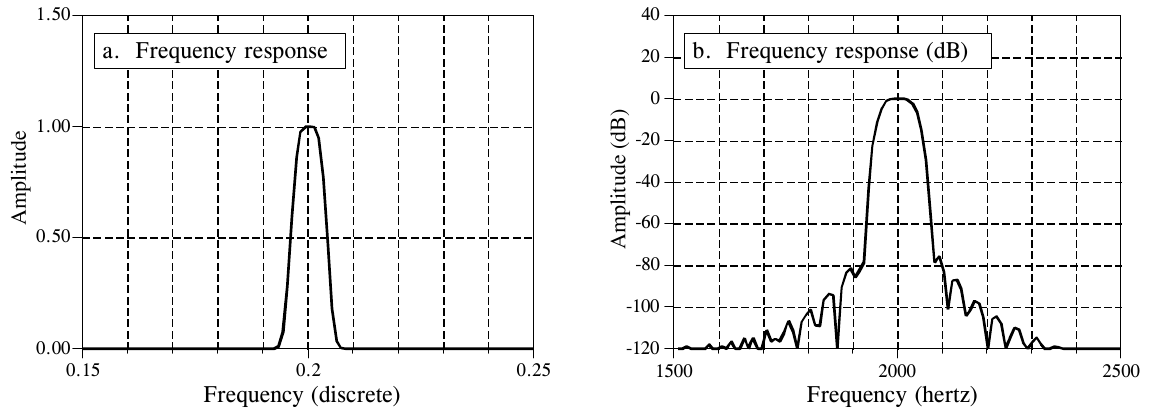
\includegraphics[width=0.958\linewidth,height=0.8\textheight,keepaspectratio]{assets/ch16/fig16-06.png}
\caption*{\textbf{图 16-6　加窗 sinc 带通滤波器的例子。} 这个滤波器是按 10 kHz
采样率设计的。对应到模拟信号，通带中心频率在 2 kHz，通带宽 80
赫兹，过渡带宽 50 赫兹。加窗 sinc 的滤波器核用了 801
个点来达到这样的滚降，并用布莱克曼窗获得良好的阻带衰减。(a)
是线性刻度的频率响应，(b) 是分贝刻度。(a)
的频率轴用采样频率的分数表示，(b) 则用数字化之前模拟信号的频率表示。
（a. Frequency response = 频率响应，b. Frequency response (dB) =
频率响应（分贝）；Frequency (discrete) = 频率（离散），Frequency (hertz)
= 频率（赫兹），Amplitude (dB) = 幅度（分贝）。(b) 纵轴 0
下面的刻度在原书图中显示为 ``20''，应为 −20。）}
\end{figure}

\textbf{表 16-2}（注释已译成中文）

\begin{Shaded}
\begin{Highlighting}[]
\NormalTok{100 \textquotesingle{}BAND{-}PASS WINDOWED{-}SINC FILTER}
\NormalTok{110 \textquotesingle{}本程序计算一个 801 点的带通滤波器核}
\NormalTok{120 \textquotesingle{}}
\NormalTok{130 DIM A[800]                      \textquotesingle{}A[ ] 是下截止频率的工作区}
\NormalTok{140 DIM B[800]                      \textquotesingle{}B[ ] 是上截止频率的工作区}
\NormalTok{150 DIM H[800]                      \textquotesingle{}H[ ] 存放最终的滤波器核}
\NormalTok{160 \textquotesingle{}}
\NormalTok{170 PI = 3.1415926}
\NormalTok{180 M\% = 800                        \textquotesingle{}设定滤波器核长度（801 点）}
\NormalTok{190 \textquotesingle{}}
\NormalTok{200 \textquotesingle{}                               \textquotesingle{}按公式 16{-}4 计算第一个低通滤波器核，}
\NormalTok{210 FC = 0.196                      \textquotesingle{}截止频率 0.196，存在 A[ ]}
\NormalTok{220 FOR I\% = 0 TO 800}
\NormalTok{230 IF (I\%{-}M\%/2) = 0 THEN A[I\%] = 2*PI*FC}
\NormalTok{240 IF (I\%{-}M\%/2) \textless{}\textgreater{} 0 THEN A[I\%] = SIN(2*PI*FC * (I\%{-}M\%/2)) / (I\%{-}M\%/2)}
\NormalTok{250 A[I\%] = A[I\%] * (0.42 {-} 0.5*COS(2*PI*I\%/M\%) + 0.08*COS(4*PI*I\%/M\%))}
\NormalTok{260 NEXT I\%}
\NormalTok{270 \textquotesingle{}}
\NormalTok{280 SUM = 0                         \textquotesingle{}把第一个低通滤波器核归一化，}
\NormalTok{290 FOR I\% = 0 TO 800               \textquotesingle{}使直流增益为 1}
\NormalTok{300 SUM = SUM + A[I\%]}
\NormalTok{310 NEXT I\%}
\NormalTok{320 \textquotesingle{}}
\NormalTok{330 FOR I\% = 0 TO 800}
\NormalTok{340 A[I\%] = A[I\%] / SUM}
\NormalTok{350 NEXT I\%}
\NormalTok{360 \textquotesingle{}                               \textquotesingle{}按公式 16{-}4 计算第二个低通滤波器核，}
\NormalTok{370 FC = 0.204                      \textquotesingle{}截止频率 0.204，存在 B[ ]}
\NormalTok{380 FOR I\% = 0 TO 800}
\NormalTok{390 IF (I\%{-}M\%/2) = 0 THEN B[I\%] = 2*PI*FC}
\NormalTok{400 IF (I\%{-}M\%/2) \textless{}\textgreater{} 0 THEN B[I\%] = SIN(2*PI*FC * (I\%{-}M\%/2)) / (I\%{-}M\%/2)}
\NormalTok{410 B[I\%] = B[I\%] * (0.42 {-} 0.5*COS(2*PI*I\%/M\%) + 0.08*COS(4*PI*I\%/M\%))}
\NormalTok{420 NEXT I\%}
\NormalTok{430 \textquotesingle{}}
\NormalTok{440 SUM = 0                         \textquotesingle{}把第二个低通滤波器核归一化，}
\NormalTok{450 FOR I\% = 0 TO 800               \textquotesingle{}使直流增益为 1}
\NormalTok{460 SUM = SUM + B[I\%]}
\NormalTok{470 NEXT I\%}
\NormalTok{480 \textquotesingle{}}
\NormalTok{490 FOR I\% = 0 TO 800}
\NormalTok{500 B[I\%] = B[I\%] / SUM}
\NormalTok{510 NEXT I\%}
\NormalTok{520 \textquotesingle{}}
\NormalTok{530 FOR I\% = 0 TO 800               \textquotesingle{}用频谱反转把 B[ ] 中的低通滤波器核}
\NormalTok{540 B[I\%] = {-} B[I\%]                 \textquotesingle{}变成高通滤波器核（如图 14{-}5）}
\NormalTok{550 NEXT I\%}
\NormalTok{560 B[400] = B[400] + 1}
\NormalTok{570 \textquotesingle{}}
\NormalTok{580 \textquotesingle{}}
\NormalTok{590 FOR I\% = 0 TO 800               \textquotesingle{}把 A[ ] 中的低通滤波器核与 B[ ] 中的高通}
\NormalTok{600 H[I\%] = A[I\%] + B[I\%]           \textquotesingle{}滤波器核相加，得到带阻滤波器核，}
\NormalTok{610 NEXT I\%                         \textquotesingle{}存在 H[ ] 中（如图 14{-}8）}
\NormalTok{620 \textquotesingle{}}
\NormalTok{630 FOR I\% = 0 TO 800               \textquotesingle{}用频谱反转把带阻滤波器核}
\NormalTok{640 H[I\%] = {-}H[I\%]                  \textquotesingle{}变成带通滤波器核}
\NormalTok{650 NEXT I\%}
\NormalTok{660 H[400] = H[400] + 1}
\NormalTok{670 \textquotesingle{}                               \textquotesingle{}带通滤波器核现在存放在 H[ ] 中}
\NormalTok{680 END}
\end{Highlighting}
\end{Shaded}

\begin{quote}
\textbf{译注：} 第 540 行注释说频谱反转''如图
14-5''，而正文讲同一步骤时引的是''第 14 章图
14-6''，两处图号不同，但都没错：第 14 章里图 14-5
是频谱反转的例子（滤波器核与频率响应），图 14-6
是频谱反转的框图，讲的是同一件事。
\end{quote}

\textbf{C 实现}（完整可编译版本见
\texttt{c/table16-2\_bandpass\_windowed\_sinc.c}，程序最后直接计算滤波器核的频率响应）：

\begin{Shaded}
\begin{Highlighting}[]
\CommentTok{/* 第 200～350 行（以及 360～510 行）：按公式 16{-}4 算低通核（布莱克曼窗），归一化到直流增益为 1 */}
\DataTypeTok{static} \DataTypeTok{void}\NormalTok{ lowpass\_kernel}\OperatorTok{(}\DataTypeTok{double}\NormalTok{ fc}\OperatorTok{,} \DataTypeTok{double} \OperatorTok{*}\NormalTok{a}\OperatorTok{)}
\OperatorTok{\{}
    \ControlFlowTok{for} \OperatorTok{(}\DataTypeTok{int}\NormalTok{ i }\OperatorTok{=} \DecValTok{0}\OperatorTok{;}\NormalTok{ i }\OperatorTok{\textless{}=}\NormalTok{ M}\OperatorTok{;}\NormalTok{ i}\OperatorTok{++)} \OperatorTok{\{}          \CommentTok{/* 220 */}
        \ControlFlowTok{if} \OperatorTok{(}\NormalTok{i }\OperatorTok{{-}}\NormalTok{ M }\OperatorTok{/} \DecValTok{2} \OperatorTok{==} \DecValTok{0}\OperatorTok{)}\NormalTok{ a}\OperatorTok{[}\NormalTok{i}\OperatorTok{]} \OperatorTok{=} \FloatTok{2.0} \OperatorTok{*}\NormalTok{ PI }\OperatorTok{*}\NormalTok{ fc}\OperatorTok{;}                             \CommentTok{/* 230 */}
        \ControlFlowTok{else}\NormalTok{                a}\OperatorTok{[}\NormalTok{i}\OperatorTok{]} \OperatorTok{=}\NormalTok{ sin}\OperatorTok{(}\FloatTok{2.0} \OperatorTok{*}\NormalTok{ PI }\OperatorTok{*}\NormalTok{ fc }\OperatorTok{*} \OperatorTok{(}\NormalTok{i }\OperatorTok{{-}}\NormalTok{ M }\OperatorTok{/} \DecValTok{2}\OperatorTok{))} \OperatorTok{/} \OperatorTok{(}\NormalTok{i }\OperatorTok{{-}}\NormalTok{ M }\OperatorTok{/} \DecValTok{2}\OperatorTok{);} \CommentTok{/* 240 */}
\NormalTok{        a}\OperatorTok{[}\NormalTok{i}\OperatorTok{]} \OperatorTok{*=} \FloatTok{0.42} \OperatorTok{{-}} \FloatTok{0.5} \OperatorTok{*}\NormalTok{ cos}\OperatorTok{(}\FloatTok{2.0} \OperatorTok{*}\NormalTok{ PI }\OperatorTok{*}\NormalTok{ i }\OperatorTok{/}\NormalTok{ M}\OperatorTok{)} \OperatorTok{+} \FloatTok{0.08} \OperatorTok{*}\NormalTok{ cos}\OperatorTok{(}\FloatTok{4.0} \OperatorTok{*}\NormalTok{ PI }\OperatorTok{*}\NormalTok{ i }\OperatorTok{/}\NormalTok{ M}\OperatorTok{);} \CommentTok{/* 250：布莱克曼窗（公式 16{-}2） */}
    \OperatorTok{\}}
    \DataTypeTok{double}\NormalTok{ sum }\OperatorTok{=} \FloatTok{0.0}\OperatorTok{;}                       \CommentTok{/* 280～310 */}
    \ControlFlowTok{for} \OperatorTok{(}\DataTypeTok{int}\NormalTok{ i }\OperatorTok{=} \DecValTok{0}\OperatorTok{;}\NormalTok{ i }\OperatorTok{\textless{}=}\NormalTok{ M}\OperatorTok{;}\NormalTok{ i}\OperatorTok{++)}\NormalTok{ sum }\OperatorTok{+=}\NormalTok{ a}\OperatorTok{[}\NormalTok{i}\OperatorTok{];}
    \ControlFlowTok{for} \OperatorTok{(}\DataTypeTok{int}\NormalTok{ i }\OperatorTok{=} \DecValTok{0}\OperatorTok{;}\NormalTok{ i }\OperatorTok{\textless{}=}\NormalTok{ M}\OperatorTok{;}\NormalTok{ i}\OperatorTok{++)}\NormalTok{ a}\OperatorTok{[}\NormalTok{i}\OperatorTok{]} \OperatorTok{/=}\NormalTok{ sum}\OperatorTok{;}   \CommentTok{/* 330～350 */}
\OperatorTok{\}}

\CommentTok{/* 频谱反转：所有采样取反，再在对称中心加 1（低通 ↔ 高通，带阻 ↔ 带通） */}
\DataTypeTok{static} \DataTypeTok{void}\NormalTok{ spectral\_inversion}\OperatorTok{(}\DataTypeTok{double} \OperatorTok{*}\NormalTok{h}\OperatorTok{)}
\OperatorTok{\{}
    \ControlFlowTok{for} \OperatorTok{(}\DataTypeTok{int}\NormalTok{ i }\OperatorTok{=} \DecValTok{0}\OperatorTok{;}\NormalTok{ i }\OperatorTok{\textless{}=}\NormalTok{ M}\OperatorTok{;}\NormalTok{ i}\OperatorTok{++)}\NormalTok{ h}\OperatorTok{[}\NormalTok{i}\OperatorTok{]} \OperatorTok{=} \OperatorTok{{-}}\NormalTok{h}\OperatorTok{[}\NormalTok{i}\OperatorTok{];}
\NormalTok{    h}\OperatorTok{[}\NormalTok{M }\OperatorTok{/} \DecValTok{2}\OperatorTok{]} \OperatorTok{+=} \FloatTok{1.0}\OperatorTok{;}
\OperatorTok{\}}

    \CommentTok{/* main() 中的主体 */}
\NormalTok{    lowpass\_kernel}\OperatorTok{(}\FloatTok{0.196}\OperatorTok{,}\NormalTok{ a}\OperatorTok{);}               \CommentTok{/* 210：第一个低通，截止 0.196，存在 A[ ] */}
\NormalTok{    lowpass\_kernel}\OperatorTok{(}\FloatTok{0.204}\OperatorTok{,}\NormalTok{ b}\OperatorTok{);}               \CommentTok{/* 370：第二个低通，截止 0.204，存在 B[ ] */}
\NormalTok{    spectral\_inversion}\OperatorTok{(}\NormalTok{b}\OperatorTok{);}                  \CommentTok{/* 530～560：B[ ] 反转成高通 */}
    \ControlFlowTok{for} \OperatorTok{(}\DataTypeTok{int}\NormalTok{ i }\OperatorTok{=} \DecValTok{0}\OperatorTok{;}\NormalTok{ i }\OperatorTok{\textless{}=}\NormalTok{ M}\OperatorTok{;}\NormalTok{ i}\OperatorTok{++)}            \CommentTok{/* 590～610：低通 + 高通 = 带阻，存在 H[ ] */}
\NormalTok{        h}\OperatorTok{[}\NormalTok{i}\OperatorTok{]} \OperatorTok{=}\NormalTok{ a}\OperatorTok{[}\NormalTok{i}\OperatorTok{]} \OperatorTok{+}\NormalTok{ b}\OperatorTok{[}\NormalTok{i}\OperatorTok{];}
\NormalTok{    spectral\_inversion}\OperatorTok{(}\NormalTok{h}\OperatorTok{);}                  \CommentTok{/* 630～660：带阻反转成带通 */}
\end{Highlighting}
\end{Shaded}

运行结果： - 通带中心 2000 Hz（0.200）处幅度 0.9998；两个截止点 1960 Hz
和 2040 Hz 处都是 0.5000（−6.0 dB），正好是半幅点。 - 离截止点 25
Hz（1935 Hz、2065 Hz）处约 −39 dB，即 1\% 左右，说明 99\%\dspsym{→}1\%
的过渡带宽约 50 Hz，与公式 16-3 的 \(M \approx 4/BW\)（4/800 =
0.005）一致。 - 离截止点 50 Hz 以外的阻带，最大残留约 −75.6
dB，与正文说的布莱克曼窗阻带衰减 −74 dB 吻合；直流处约 −300
dB，等于完全挡住。

\section{把性能推到极限}

加窗 sinc
滤波器的性能可以推到惊人的高度，而不出令人难堪的意外。例如，假设你需要从一条
120 伏的电源线上分离出一个 1 毫伏的信号。低通滤波器需要至少 −120 dB
的阻带衰减（对那些不肯学分贝的人来说，就是百万分之一）。前面说过，布莱克曼窗只能提供
−74 dB（五千分之一）。幸好，更大的阻带衰减很容易得到。可以先用普通的加窗
sinc
滤波器核对输入信号滤波，得到一个中间信号；再让这个中间信号第二次通过这个滤波器，阻带衰减就能进一步提高到
−148
dB（三千万分之一，哇！）。也可以把两级合并成一个滤波器：合并后滤波器的核，等于两级滤波器核的卷积。这也意味着，任何滤波器核与自身卷积，都会得到一个阻带衰减大大改善的滤波器核。代价是滤波器核更长、滚降更慢。图
16-7a 是一个 201 点低通滤波器的频率响应，它由一个 101 点的布莱克曼加窗
sinc 与自身卷积而成。惊人的性能！（如果你真的需要超过 −100 dB
的阻带衰减，就应该用双精度。单精度下，通带中信号的舍入噪声可能会不规则地出现在阻带里，幅度在
−100 dB 到 −120 dB 之间。）

\begin{figure}[htbp]
\centering
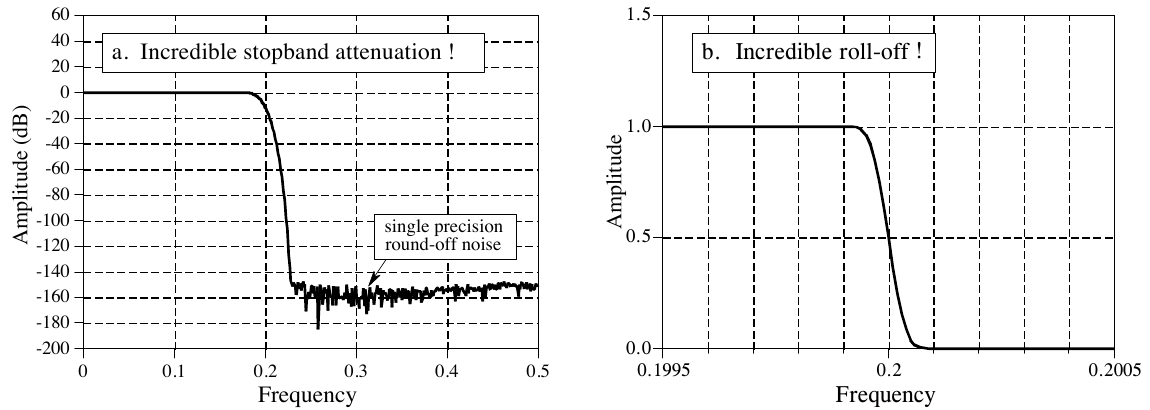
\includegraphics[width=0.958\linewidth,height=0.8\textheight,keepaspectratio]{assets/ch16/fig16-07.png}
\caption*{\textbf{图 16-7　加窗 sinc 滤波器惊人的性能。} (a)
是一个阻带衰减增强的加窗 sinc 滤波器的频率响应，这是把加窗 sinc
滤波器核与自身卷积得到的。(b) 是一个 32,001 点加窗 sinc
滤波器极快的滚降。 （a. Incredible stopband attenuation ! =
惊人的阻带衰减！b. Incredible roll-off ! = 惊人的滚降！single precision
round-off noise = 单精度舍入噪声。Amplitude = 幅度，Amplitude (dB) =
幅度（分贝），Frequency = 频率。）}
\end{figure}

图 16-7b 是加窗 sinc 惊人性能的另一个例子：一个滤波器核有 32,001
个点的低通滤波器。频率响应和预期的一样，滚降宽度是采样率的
0.000125。这个滤波器有多好？试着做一个模拟电子滤波器：让直流到 1000
赫兹的信号通过、变化小于 0.02\%，同时挡住 1001
赫兹以上的所有频率、残留小于
0.02\%。那才叫滤波器！如果你真想被震撼一下，记住图 16-7
中的两个滤波器都用的是单精度。用双精度还能把这些性能指标再扩展一百万倍。

加窗 sinc
滤波器最大的局限是执行时间：如果滤波器核点数很多，又用标准卷积，执行时间可能长得无法接受。第
18 章会介绍这种滤波器的一种高速算法（FFT 卷积）。递归滤波器（recursive
filter，第 19 章）也能提供良好的频率分离，是加窗 sinc
滤波器的一个合理替代。

加窗 sinc
是分离频率的最优滤波器核吗？不是，更复杂的技术得到的滤波器核可以更好。但要当心！在一头扎进这个非常数学化的领域之前，你应该想清楚自己到底想得到什么。加窗
sinc
能提供你可能需要的任何性能水平。高级滤波器设计方法能提供的，也许只是在给定性能下稍短一点的滤波器核，进而也许稍快一点的执行速度。要有心理准备：你付出的努力可能换不来多少回报。

% !TEX root = ../main.tex
% 本文件由 build-tex.sh 从 17-DSP指南-第17章中译.md 生成，改内容请改 md 后重新生成

\chapter{自定义滤波器}\label{ch-17}

大多数滤波器的频率响应属于四种标准类型之一：低通、高通、带通或带阻。本章介绍一种通用方法，用来设计具有任意频率响应的数字滤波器，按你具体应用的需要量身定做。DSP
在这方面表现出色，能解决远远超出模拟电子学能力的问题。本章讨论自定义滤波器的两个重要用途：反卷积(deconvolution)，即恢复经历过不想要的卷积的信号；以及最优滤波(optimal
filtering)，即分离频谱相互重叠的信号的问题。这是 DSP 最精彩的地方。

\section{任意频率响应}

上一章推导加窗 sinc 滤波器(windowed-sinc
filter)的方法，也可以用来设计几乎任何频率响应的滤波器。唯一的区别在于怎样把期望的响应从频域搬到时域。在加窗
sinc
滤波器中，频率响应和滤波器核都用公式表示，两者之间的转换靠计算傅里叶变换的数学来完成。而在这里介绍的方法中，两个信号都用数字数组表示，用一个计算机程序（FFT）由其中一个求出另一个。

图 17-1 是一个例子，说明这个方法怎样运作。我们想让滤波器产生的频率响应如
(a)
所示。说得客气点，它非常不规则，用模拟电子学几乎不可能做到。这个理想频率响应由一组挑选出来的数字定义，而不是某个数学公式。本例中，在采样率的
0 到 0.5 之间分布着 513
个采样。可以用更多的点来更好地表示期望的频率响应，也可能需要用更少的点来缩短滤波器设计时的计算时间。不过，这些顾虑通常都不大，513
对大多数应用来说是个合适的长度。

除了 (a)
所示的期望幅度数组，还必须有一个同样长度的相位数组与之对应。本例中，期望频率响应的相位全为零（图
17-1
没有画出这个数组）。和幅度数组一样，相位数组也可以装入任何你想让滤波器产生的曲线。不过要记住，相位数组的第一个和最后一个采样（即第
0 和第 512 个）的值必须为零（或者 2π
的整数倍，这是一回事）。频率响应也可以用直角坐标形式指定，即给出实部和虚部数组的各项，而不用幅度和相位。

下一步是做逆
DFT，把滤波器搬到时域。最快的办法是把频域转换成直角坐标形式，然后用逆
FFT。得到一个从 0 到 1023 的 1024 点信号，如 (b)
所示。这就是与我们想要的频率响应相对应的冲激响应；不过，它并不适合直接用作滤波器核（稍后详谈）。和上一章一样，它需要经过平移、截断和加窗。本例中，我们设计
\(M = 40\) 的滤波器核，即从第 0 到第 40 个采样共 41 个点。表 17-1
给出了把 (b) 中的信号变成 (c) 所示滤波器核的程序。和加窗 sinc
滤波器一样，滤波器核两端附近的点非常小，画出来看起来就是零。千万别误以为可以把它们删掉！

\textbf{表 17-1}（注释已译成中文）

\begin{Shaded}
\begin{Highlighting}[]
\NormalTok{100 \textquotesingle{}CUSTOM FILTER DESIGN（自定义滤波器设计）}
\NormalTok{110 \textquotesingle{}本程序把一个 1024 点的混叠冲激响应转换成 M+1 点的}
\NormalTok{120 \textquotesingle{}滤波器核（例如把图 17{-}1b 转换成图 17{-}1c）}
\NormalTok{130 \textquotesingle{}}
\NormalTok{140 DIM REX[1023]                      \textquotesingle{}REX[ ] 存放要转换的信号}
\NormalTok{150 DIM T[1023]                        \textquotesingle{}T[ ] 是临时存储缓冲区}
\NormalTok{160 \textquotesingle{}}
\NormalTok{170 PI = 3.14159265}
\NormalTok{180 M\% = 40                            \textquotesingle{}设定滤波器核长度（共 41 个点）}
\NormalTok{190 \textquotesingle{}}
\NormalTok{200 GOSUB XXXX                         \textquotesingle{}虚构的子程序，把冲激响应载入 REX[ ]}
\NormalTok{210 \textquotesingle{}}
\NormalTok{220 FOR I\% = 0 TO 1023                 \textquotesingle{}把信号向右平移（循环移位）M/2 点}
\NormalTok{230 INDEX\% = I\% + M\%/2}
\NormalTok{240 IF INDEX\% \textgreater{} 1023 THEN INDEX\% = INDEX\%{-}1024}
\NormalTok{250 T[INDEX\%] = REX[I\%]}
\NormalTok{260 NEXT I\%}
\NormalTok{270 \textquotesingle{}}
\NormalTok{280 FOR I\% = 0 TO 1023}
\NormalTok{290 REX[I\%] = T[I\%]}
\NormalTok{300 NEXT I\%}
\NormalTok{310 \textquotesingle{}                                  \textquotesingle{}截断信号并加窗}
\NormalTok{320 FOR I\% = 0 TO 1023}
\NormalTok{330 IF I\% \textless{}= M\% THEN REX[I\%] = REX[I\%] * (0.54 {-} 0.46 * COS(2*PI*I\%/M\%))}
\NormalTok{340 IF I\% \textgreater{} M\% THEN REX[I\%] = 0}
\NormalTok{350 NEXT I\%}
\NormalTok{360 \textquotesingle{}                                  \textquotesingle{}滤波器核现在位于 REX[0] 到 REX[40]}
\NormalTok{370 END}
\end{Highlighting}
\end{Shaded}

\textbf{C 实现}（完整可编译版本见
\texttt{c/table17-1\_custom\_filter.c}。原书第 200
行用虚构的子程序载入信号，C 版本把前后两步也补上了：按图 17-1a
的形状定义期望频率响应，逆 DFT 得到混叠冲激响应，执行表
17-1，再求实际频率响应与期望值比较）：

\begin{Shaded}
\begin{Highlighting}[]
\DataTypeTok{static} \DataTypeTok{void}\NormalTok{ custom\_filter\_kernel}\OperatorTok{(}\DataTypeTok{double} \OperatorTok{*}\NormalTok{rex}\OperatorTok{,} \DataTypeTok{int}\NormalTok{ m}\OperatorTok{)}
\OperatorTok{\{}
    \DataTypeTok{double}\NormalTok{ t}\OperatorTok{[}\NormalTok{N}\OperatorTok{];}                            \CommentTok{/* 150 DIM T[1023]：临时缓冲区 */}

    \ControlFlowTok{for} \OperatorTok{(}\DataTypeTok{int}\NormalTok{ i }\OperatorTok{=} \DecValTok{0}\OperatorTok{;}\NormalTok{ i }\OperatorTok{\textless{}}\NormalTok{ N}\OperatorTok{;}\NormalTok{ i}\OperatorTok{++)} \OperatorTok{\{}           \CommentTok{/* 220～260：把信号循环右移 M/2 点 */}
        \DataTypeTok{int}\NormalTok{ index }\OperatorTok{=}\NormalTok{ i }\OperatorTok{+}\NormalTok{ m }\OperatorTok{/} \DecValTok{2}\OperatorTok{;}              \CommentTok{/* 230 */}
        \ControlFlowTok{if} \OperatorTok{(}\NormalTok{index }\OperatorTok{\textgreater{}}\NormalTok{ N }\OperatorTok{{-}} \DecValTok{1}\OperatorTok{)}\NormalTok{ index }\OperatorTok{{-}=}\NormalTok{ N}\OperatorTok{;}      \CommentTok{/* 240：超出末尾的绕回开头 */}
\NormalTok{        t}\OperatorTok{[}\NormalTok{index}\OperatorTok{]} \OperatorTok{=}\NormalTok{ rex}\OperatorTok{[}\NormalTok{i}\OperatorTok{];}                  \CommentTok{/* 250 */}
    \OperatorTok{\}}
    \ControlFlowTok{for} \OperatorTok{(}\DataTypeTok{int}\NormalTok{ i }\OperatorTok{=} \DecValTok{0}\OperatorTok{;}\NormalTok{ i }\OperatorTok{\textless{}}\NormalTok{ N}\OperatorTok{;}\NormalTok{ i}\OperatorTok{++)}             \CommentTok{/* 280～300：拷回 REX[ ] */}
\NormalTok{        rex}\OperatorTok{[}\NormalTok{i}\OperatorTok{]} \OperatorTok{=}\NormalTok{ t}\OperatorTok{[}\NormalTok{i}\OperatorTok{];}

    \ControlFlowTok{for} \OperatorTok{(}\DataTypeTok{int}\NormalTok{ i }\OperatorTok{=} \DecValTok{0}\OperatorTok{;}\NormalTok{ i }\OperatorTok{\textless{}}\NormalTok{ N}\OperatorTok{;}\NormalTok{ i}\OperatorTok{++)} \OperatorTok{\{}           \CommentTok{/* 320～350：截断并加窗 */}
        \ControlFlowTok{if} \OperatorTok{(}\NormalTok{i }\OperatorTok{\textless{}=}\NormalTok{ m}\OperatorTok{)}\NormalTok{ rex}\OperatorTok{[}\NormalTok{i}\OperatorTok{]} \OperatorTok{*=} \FloatTok{0.54} \OperatorTok{{-}} \FloatTok{0.46} \OperatorTok{*}\NormalTok{ cos}\OperatorTok{(}\FloatTok{2.0} \OperatorTok{*}\NormalTok{ PI }\OperatorTok{*}\NormalTok{ i }\OperatorTok{/}\NormalTok{ m}\OperatorTok{);}  \CommentTok{/* 330：汉明窗 */}
        \ControlFlowTok{else}\NormalTok{        rex}\OperatorTok{[}\NormalTok{i}\OperatorTok{]} \OperatorTok{=} \FloatTok{0.0}\OperatorTok{;}           \CommentTok{/* 340：M 之后的点全部置零 */}
    \OperatorTok{\}}
\OperatorTok{\}}                                           \CommentTok{/* 360：滤波器核现在位于 REX[0]～REX[M] */}
\end{Highlighting}
\end{Shaded}

运行结果（实际频率响应与期望频率响应在 513 个设计点上的偏差）：

{\def\LTcaptype{none} % do not increment counter
\begin{longtable}[]{@{}lll@{}}
\toprule\noalign{}
M & 偏差的均方根 & 最大偏差 \\
\midrule\noalign{}
\endhead
\bottomrule\noalign{}
\endlastfoot
10 & 0.399 & 1.33 \\
30 & 0.248 & 0.93 \\
40 & 0.218 & 0.87 \\
100 & 0.125 & 0.76 \\
300 & 0.068 & 0.64 \\
1000 & 0.030 & 0.36 \\
\end{longtable}
}

滤波器核越长，实际响应越贴近期望响应，和图 17-2
的趋势一致；剩下的最大偏差集中在期望响应的陡峭跳变处（比如 0.195 处从
2.5 跌到 1、0.27～0.29
的窄阻带）。程序最后还验证了本节末尾的论点：直接拿 1024
点混叠冲激响应当滤波器核，在 513 个设计点上与期望值的偏差只有
1.8e-13，但在相邻设计点正中间，偏差最大达到 1.49；按表 17-1 加窗后（M =
1000），设计点之间的最大偏差降到 0.098。

\begin{figure}[htbp]
\centering
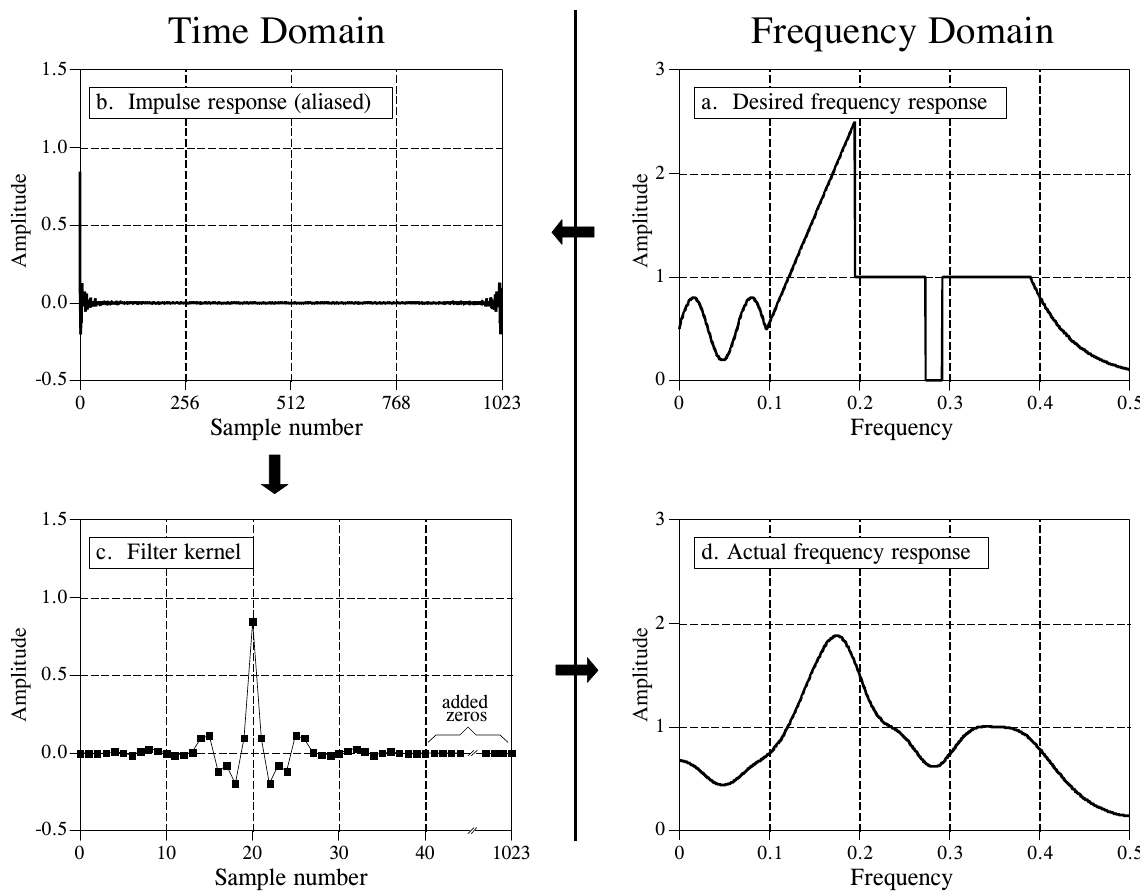
\includegraphics[width=0.950\linewidth,height=0.8\textheight,keepaspectratio]{assets/ch17/fig17-01.png}
\caption*{\textbf{图 17-1　FIR 滤波器设计示例。} (a) 是期望的频率响应，有 513
个采样，分布在采样率的 0 到 0.5 之间。做逆 DFT 得到 (b)，一个由 1024
个采样组成的混叠冲激响应。为了得到滤波器核 (c)，把混叠冲激响应截断为 M+1
个采样、向右平移 M/2 个采样，再乘以汉明窗或布莱克曼窗。本例中 M 为
40。表 17-1 的程序展示了具体做法。检验滤波器核的方法是补零后做
DFT，得到滤波器的实际频率响应 (d)。 （Time Domain = 时域，Frequency
Domain = 频域；a. Desired frequency response = 期望频率响应；b. Impulse
response (aliased) = 冲激响应（混叠的）；c.~Filter kernel =
滤波器核；d.~Actual frequency response = 实际频率响应；added zeros =
补上的零。Amplitude = 幅度，Sample number = 采样序号，Frequency =
频率。图注说''截断\ldots\ldots 再平移''，表 17-1
程序的实际顺序是先平移、后截断。）}
\end{figure}

最后一步是检验滤波器核。做法是做 DFT（用 FFT）求出实际频率响应，如 (d)
所示。为了在频域得到更好的分辨率，在做 FFT
之前给滤波器核补零。例如，总共用 1024 个采样（滤波器核 41 个，加上 983
个零），就能在 0 到 0.5 之间得到 513 个采样。

如图 17-2
所示，滤波器核的长度决定了实际频率响应与期望频率响应吻合得多好。FIR
数字滤波器的出色性能在这里一目了然：只要滤波器核足够长，几乎任何频率响应都能得到。

\begin{figure}[htbp]
\centering
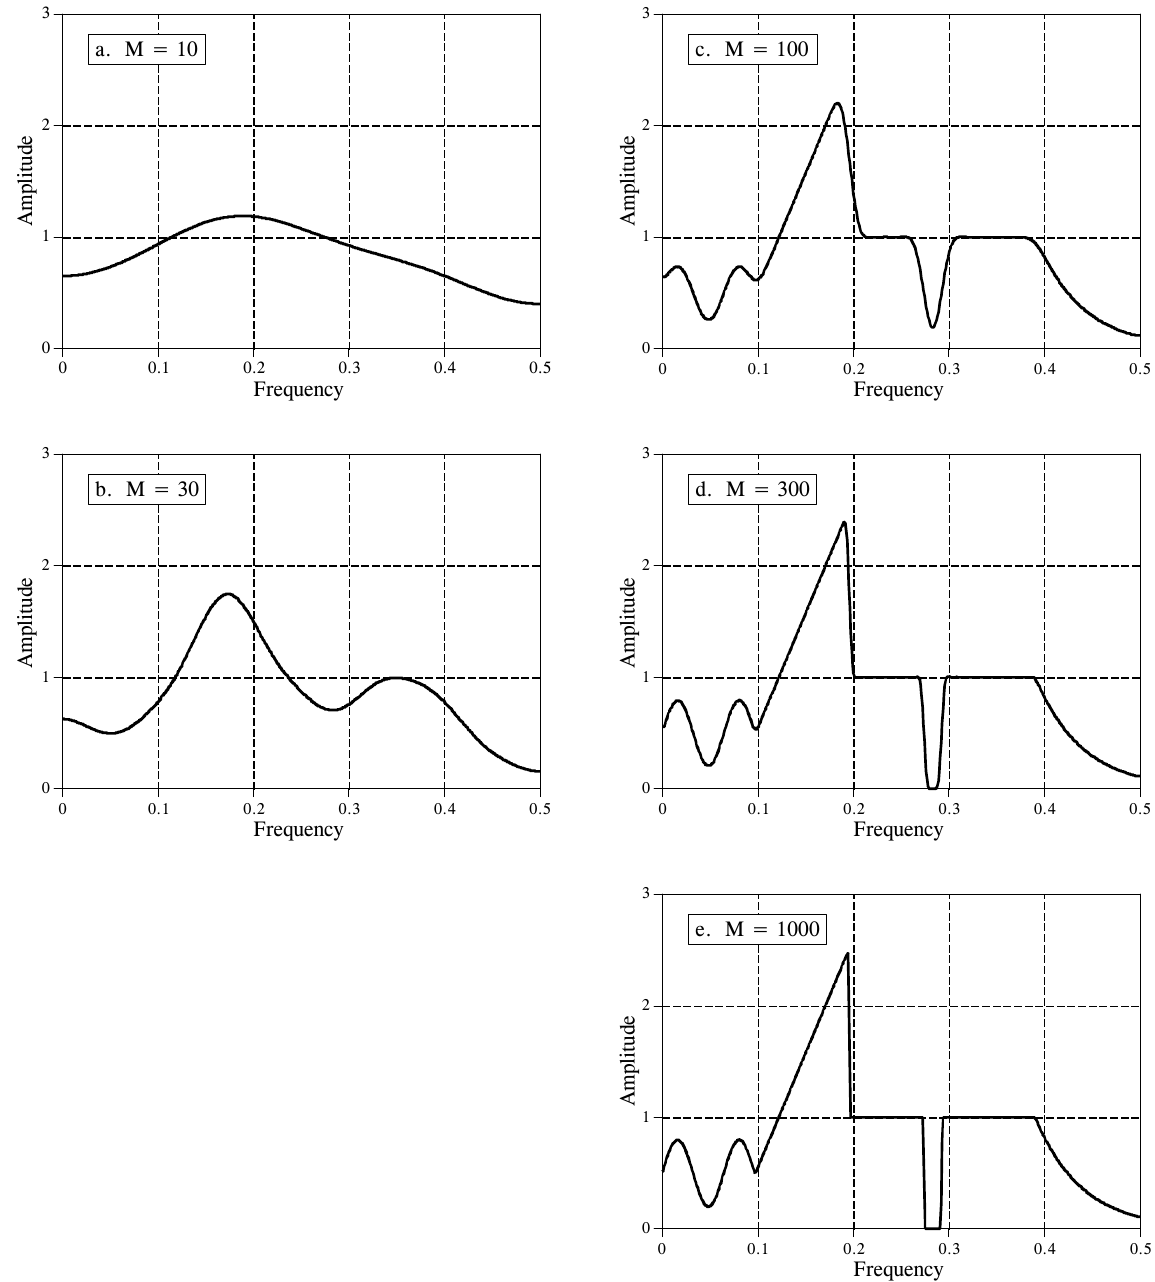
\includegraphics[width=0.963\linewidth,height=0.8\textheight,keepaspectratio]{assets/ch17/fig17-02.png}
\caption*{\textbf{图 17-2　频率响应与滤波器核长度的关系。}
这几张图展示了用不同长度的滤波器核得到的频率响应。每个滤波器核的点数等于
M+1，从 0 到
M。滤波器核用的点越多，得到的频率响应就越接近期望的频率响应。本例的期望频率响应见图
17-1a。 （a～e 依次为 M = 10、30、100、300、1000。Amplitude =
幅度，Frequency =
频率。原书图注排在左下空白处，裁图时已去掉，译文见上。）}
\end{figure}

设计方法就是这些；不过，有一个微妙的理论问题需要澄清。为什么不能直接把图
17-1b 所示的冲激响应用作滤波器核？毕竟，如果 (a) 是 (b)
的傅里叶变换，那么把输入信号与 (b)
卷积，不就能得到我们想要的那个确切的频率响应吗？答案是否定的，原因如下。

设计自定义滤波器时，期望的频率响应由一个数组里的值来定义。现在想一想：在这些指定点之间，频率响应是什么样的？为简单起见，可以设想两种情况，一种''好''，一种''坏''。在''好''的情况下，频率响应在定义的采样之间是一条平滑的曲线。在''坏''的情况下，采样之间有剧烈的起伏。不巧的是，(b)
中的冲激响应对应的恰恰是''坏''的频率响应。这一点可以这样看出：给它补上大量的零，然后做
DFT。用这种方法得到的频率响应，会在原先定义的采样之间表现出不规则的行为，看上去一塌糊涂。

要理解这一点，设想我们在 0 到 0.5
之间无穷多个点上定义频率响应，强迫它就是我们想要的样子。也就是说，我们构造了一条连续曲线。然后用逆
DTFT
求冲激响应，它的长度会是无穷的。换句话说，``好''的频率响应对应着一个计算机无法表示的东西：一个无限长的冲激响应。当我们用
N/2+1 个采样表示频谱时，时域只提供了 N
个点，没法正确容纳这个信号。结果就是，无限长的冲激响应卷绕（混叠）进这 N
个点里。一旦发生这种混叠，频率响应就从''好''变成了''坏''。幸运的是，给这
N 点冲激响应加窗可以大大减轻这种混叠，使频域采样之间成为平滑的曲线。

设计一个产生给定频率响应的数字滤波器相当简单。难的是找出该用什么样的频率响应。我们来看看
DSP 中设计自定义滤波器的一些策略。

\section{反卷积}

不想要的卷积是传输模拟信息时固有的问题。例如，下面这些都可以建模为卷积：手抖的相机拍出的图像模糊、长途电话里的回声、模拟传感器和电子器件的有限带宽，等等。反卷积是对信号做滤波、以补偿不想要的卷积的过程。反卷积的目标是重建卷积发生之前的信号。这通常要求已知卷积的特性（即冲激响应或频率响应）。这一点使它区别于盲反卷积(blind
deconvolution)，后者不知道这个寄生卷积的特性。盲反卷积是困难得多的问题，没有通用的解法，方法必须针对具体应用量身定制。

反卷积在时域几乎无法理解，但在频域却相当直观。构成原信号的每个正弦波，在经过不想要的卷积时，幅度和/或相位都可能改变。要提取原信号，反卷积滤波器必须撤销这些幅度和相位的变化。例如，如果卷积把某个正弦波的幅度变为
0.5 倍、相位移动 30 度，那么反卷积滤波器就必须把这个正弦波放大 2.0
倍、相位改变 −30 度。

我们用来说明反卷积的例子是一个伽马射线探测器(gamma ray detector)。如图
17-3 所示，这种装置由两部分组成：闪烁体(scintillator)和光探测器(light
detector)。闪烁体是一种特殊的透明材料，比如碘化钠或锗酸铋。这些化合物把每个伽马射线的能量转换成一小阵可见光。这些光再由光探测器（比如光电二极管或光电倍增管）转换成电信号。探测器产生的每个脉冲都像一个单边指数函数，只是拐角处略圆一些。这个形状由所用闪烁体的特性决定。伽马射线把能量沉积到闪烁体中时，附近的原子被激发到更高的能级。这些原子随机地退激发，每个产生一个可见光光子。最终的结果是一个光脉冲，它的幅度在几百纳秒内衰减（对碘化钠而言）。由于每个伽马射线的到达都是一个冲激，探测器输出的脉冲（即那个单边指数函数）就是这个系统的冲激响应。

\begin{figure}[htbp]
\centering
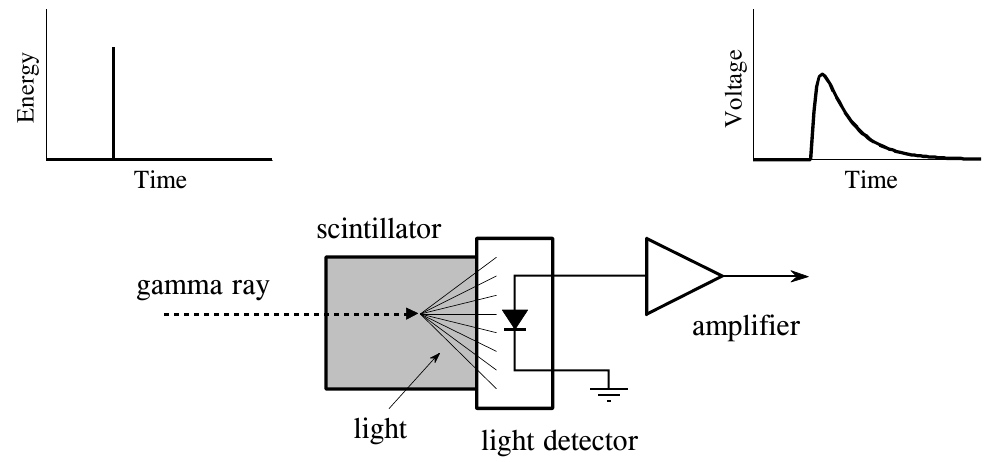
\includegraphics[width=0.833\linewidth,height=0.8\textheight,keepaspectratio]{assets/ch17/fig17-03.png}
\caption*{\textbf{图 17-3　无法避免的卷积的例子。}
把闪烁体装在光探测器上，就构成一个伽马射线探测器。伽马射线击中闪烁体时，它的能量被转换成一个光脉冲。这个光脉冲再由光探测器转换成电信号。伽马射线是一个冲激，而探测器的输出（即冲激响应）像一个单边指数函数。
（Energy = 能量，Voltage = 电压，Time = 时间；gamma ray =
伽马射线，scintillator = 闪烁体，light = 光，light detector =
光探测器，amplifier = 放大器。）}
\end{figure}

图 17-4a
是探测器对随机到达的伽马射线产生的脉冲。我们想从这个输出信号中提取的信息是每个脉冲的幅度，它与产生该脉冲的伽马射线的能量成正比。这个信息很有用，因为能量可以告诉我们这个伽马射线来自何处的有趣信息。例如，它可以提供病人的医学信息，告诉我们一个遥远星系的年龄，在航空行李中发现炸弹，等等。

如果只是偶尔探测到一个伽马射线，一切都好办，但实际情况通常不是这样。如
(a)
所示，两个或更多脉冲可能重叠，使测得的幅度发生偏移。解决这个问题的一个办法是对探测器的输出信号做反卷积，让脉冲变窄，从而减少堆积(pile-up)。理想情况下，我们希望每个脉冲都像原来的冲激。你大概也猜到了，这做不到，我们只能退而求其次，接受一个长度有限、但比探测到的脉冲短得多的脉冲。这个目标如图
17-4b 所示。

\begin{figure}[htbp]
\centering
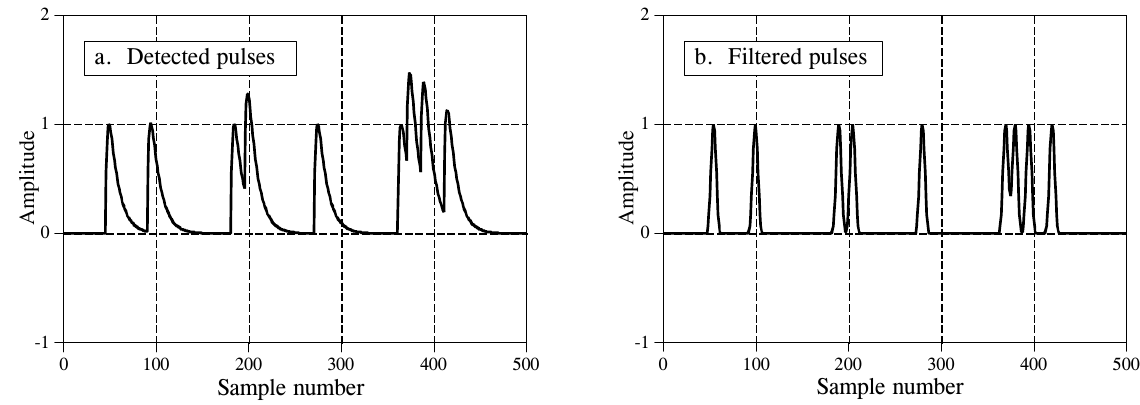
\includegraphics[width=0.950\linewidth,height=0.8\textheight,keepaspectratio]{assets/ch17/fig17-04.png}
\caption*{\textbf{图 17-4　反卷积的例子。} (a)
是伽马射线探测器对一串随机到达的伽马射线的输出信号。反卷积滤波器的设计目标是把
(a) 变成
(b)，即缩小脉冲的宽度。这样当脉冲相互叠在一起时，幅度的偏移就最小。 （a.
Detected pulses = 探测到的脉冲；b. Filtered pulses =
滤波后的脉冲。Amplitude = 幅度，Sample number = 采样序号。）}
\end{figure}

尽管探测器信号的信息编码在时域里，我们的大部分分析却必须在频域里进行，因为在那里问题更容易理解。图
17-5a 是探测器产生的信号（这是我们已知的）。(c)
是我们希望得到的信号（也是已知的）。这个期望的脉冲是随意选的，形状与布莱克曼窗相同，长度约为原脉冲的三分之一。我们的目标是找到一个滤波器核
(e)，使它与 (a) 中的信号卷积后产生 (c) 中的信号。写成公式：若
\(a * e = c\)，已知 a 和 c，求 e。

如果这些信号是用加法或乘法而不是卷积组合起来的，解法就很容易：用减法来''去加''，用除法来''去乘''。卷积则不同，并没有一种可以叫做''去卷积''的简单逆运算。卷积太复杂，无法通过直接操纵时域信号来撤销。

幸运的是，这个问题在频域里更简单。记住，一个域中的卷积对应另一个域中的乘法。仍以图
17-5 中的信号为例：若 \(b \times f = d\)，已知 b 和 d，求
f。这个问题很容易解：滤波器的频率响应 (f)，等于期望脉冲的频谱 (d)
除以探测到的脉冲的频谱
(b)。由于探测到的脉冲不对称，它的相位不为零。这意味着必须用复数除法（即一个幅度和相位除以另一个幅度和相位）。万一你忘了，第
9 章讲过怎样用一个频谱去除另一个频谱。然后用自定义滤波器的方法（逆
DFT、平移、截断、乘以窗函数），由这个频率响应求出所需的滤波器核 (e)。

\begin{figure}[htbp]
\centering
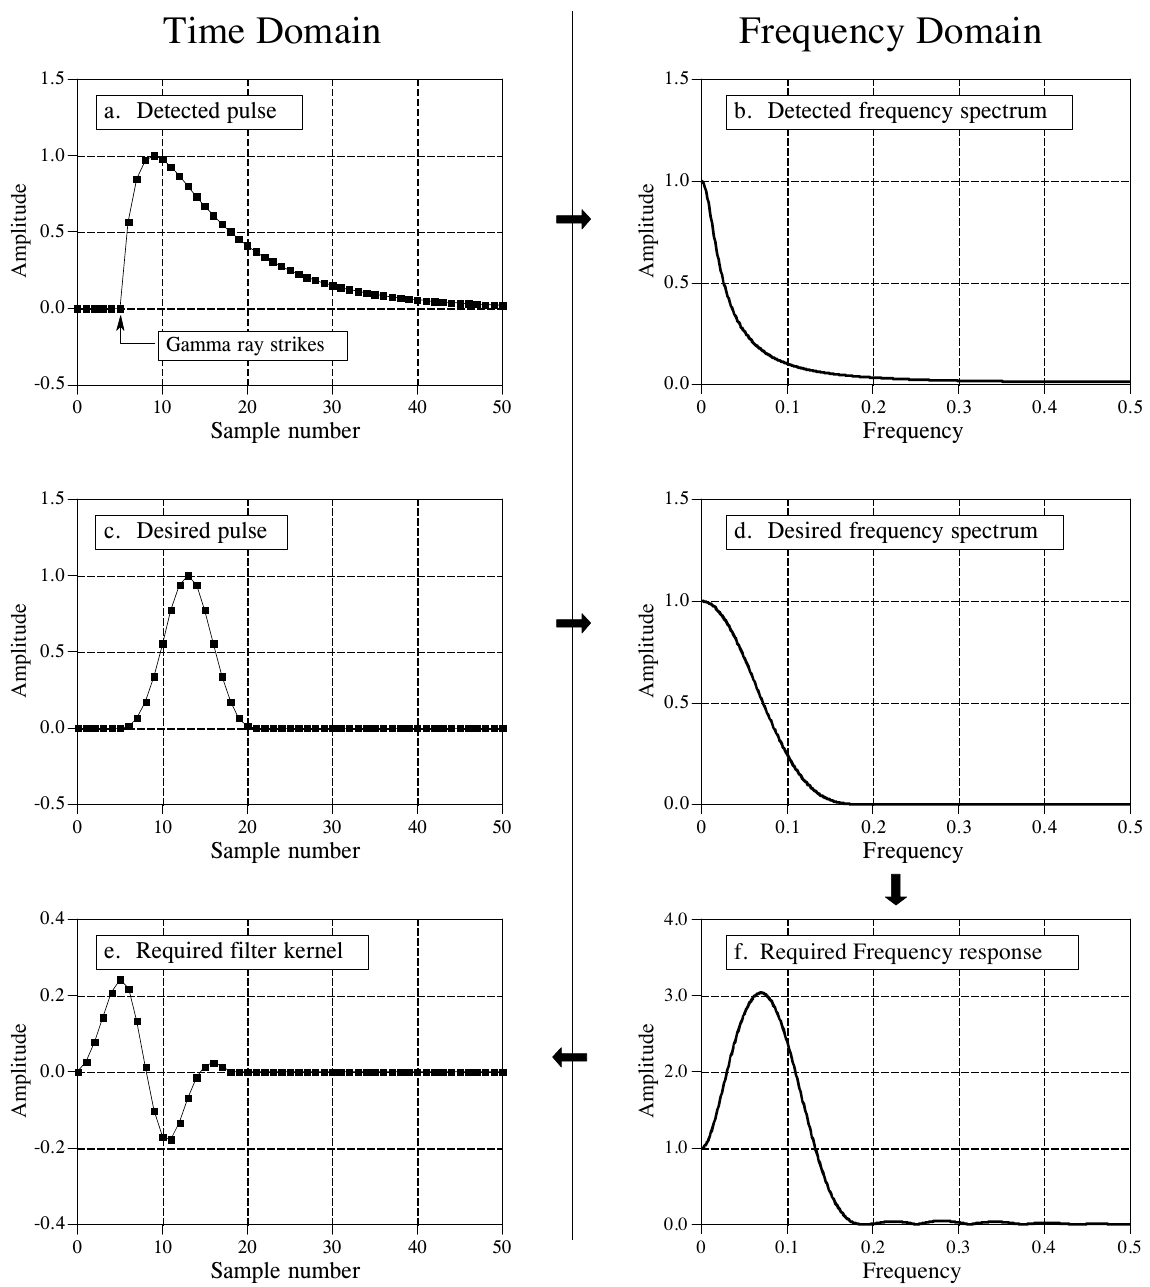
\includegraphics[width=0.958\linewidth,height=0.8\textheight,keepaspectratio]{assets/ch17/fig17-05.png}
\caption*{\textbf{图 17-5　时域和频域中的反卷积示例。}
示例伽马射线探测器的冲激响应如 (a) 所示，期望的冲激响应如 (c)
所示。这两个信号的频谱分别如 (b) 和 (d) 所示。把 (a) 变成 (c)
的滤波器，其频率响应 (f) 等于 (d) 除以 (b)。这个滤波器的核 (e)
再用自定义滤波器设计方法（逆
DFT、截断、加窗）由频率响应求出。本图只画出了频域信号的幅度；不过，它们的相位并不为零，也必须用上。
（Time Domain = 时域，Frequency Domain = 频域；a. Detected pulse =
探测到的脉冲，Gamma ray strikes = 伽马射线击中；b. Detected frequency
spectrum = 探测到的频谱；c.~Desired pulse = 期望的脉冲；d.~Desired
frequency spectrum = 期望的频谱；e. Required filter kernel =
所需的滤波器核；f.~Required Frequency response =
所需的频率响应。Amplitude = 幅度，Sample number = 采样序号，Frequency =
频率。）}
\end{figure}

\begin{quote}
\textbf{译注：} 原书图注写的是 ``(f), equal to (b) divided by (d)''，即
(b) 除以 (d)，与正文矛盾，也与图对不上：(f) 在低频处约为 1、在 0.07
附近升到约 3，只有 (d)/(b) 才是这样。这里按正文改为 (d) 除以 (b)。
\end{quote}

反卷积能带来的改善是有限度的。换句话说，如果你贪心，事情就会崩溃。在这个例子里，贪心就是想让期望的脉冲窄得过分。我们来看看会发生什么。如果期望脉冲做得更窄，它的频谱就必须包含更多的高频成分。由于这些高频成分在探测到的脉冲中幅度非常低，滤波器在这些频率上就必须有非常高的增益。例如，(f)
显示，为了得到 (c) 中的期望脉冲，有些频率必须乘以
3。如果期望脉冲做得更窄，反卷积滤波器在高频处的增益还要更大。

问题在于，在这种情况下，小误差是非常不可原谅的。例如，如果某个频率只需要放大
28 倍，却被放大了 30
倍，反卷积后的信号很可能一团糟。当反卷积被推向更高的性能水平时，对那个不想要的卷积的特性就必须了解得更准确、更精确。在现实应用中，总存在一些未知因素，来源于这样一些坏蛋：电子噪声、温度漂移、器件之间的差异等。这些未知因素限制了反卷积能做到多好。

即使完全了解那个不想要的卷积，仍然有一个因素限制反卷积的性能：噪声。例如，大多数不想要的卷积都表现为低通滤波器，降低信号中高频成分的幅度。反卷积通过放大这些频率来纠正这一点。然而，如果这些成分的幅度降到了系统固有噪声之下，这些频率中包含的信息就丢失了。再多的信号处理也找不回来。它永远消失了。Adios！Goodbye！Sayonara！试图找回这些数据只会放大噪声。极端情况下，有些频率的幅度可能完全降为零。这不仅抹掉了信息，还会使反卷积滤波器在这些频率上试图有无穷大的增益。解决办法是：设计一个不那么激进的反卷积滤波器，和/或限制任何频率上所允许的增益。

能走多远？多贪才算太贪？这完全取决于你要解决的问题。如果信号表现良好、噪声低，大概可以获得显著的改善（想想
5～10
倍）。如果信号随时间变化、了解得不是特别清楚、或者噪声大，效果就会差得多（想想
1～2
倍）。成功的反卷积需要大量的测试。如果在某个程度上奏效了，就再往前推一点；它崩溃的时候你自然会知道。再多的理论工作也不能让你绕过这个反复试验的过程。

反卷积也可以用于信息编码在频域中的信号。一个经典的例子是修复著名歌剧演唱家恩里科·卡鲁索（Enrico
Caruso，1873-1921）的老唱片。按现代标准，这些唱片是用非常原始的设备录制的。最主要的问题是用来收集声音的长管状录音喇叭的共振。每当歌手恰好唱到其中某个共振频率，录音的响度就会突然增大。数字反卷积通过压低音乐中这些过响的地方，改善了这些录音的主观听感。我们只介绍一般的方法；详细的描述请参阅原始论文：T.
Stockham, T. Cannon, and R. Ingebretsen, ``Blind Deconvolution Through
Digital Signal Processing'', Proc. IEEE, vol.~63, Apr.~1975,
pp.~678-692。

\begin{figure}[htbp]
\centering
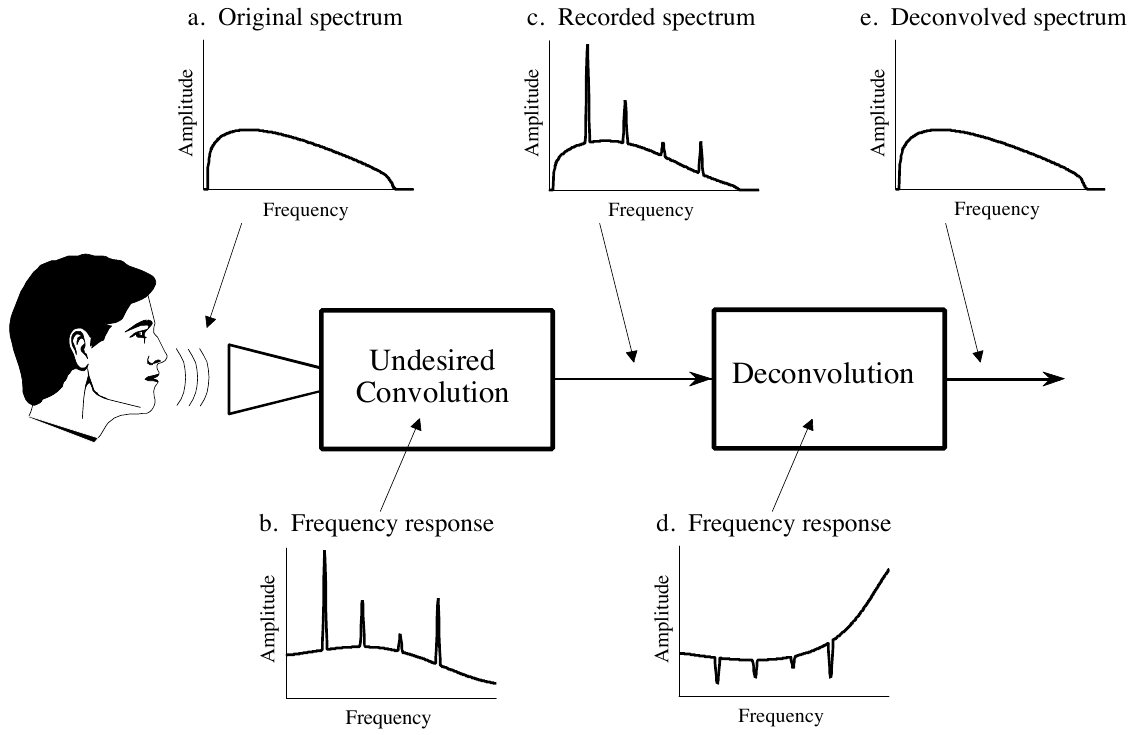
\includegraphics[width=0.950\linewidth,height=0.8\textheight,keepaspectratio]{assets/ch17/fig17-06.png}
\caption*{\textbf{图 17-6　老唱片的反卷积。} 原歌手发出的频谱如 (a)
所示。原始设备中的共振峰 (b) 使录下来的频谱 (c)
产生失真。反卷积滤波器的频率响应 (d)
用来抵消这个不想要的卷积，恢复出原始频谱
(e)。这些图仅作示意，并非真实信号。 （a. Original spectrum =
原始频谱；b. Frequency response = 频率响应；c.~Recorded spectrum =
录下的频谱；d.~Frequency response = 频率响应；e. Deconvolved spectrum =
反卷积后的频谱；Undesired Convolution = 不想要的卷积，Deconvolution =
反卷积。Amplitude = 幅度，Frequency = 频率。原书图注 ``designed to
counteracts'' 中的 counteracts 应为 counteract。）}
\end{figure}

图 17-6 展示了一般的做法。原始音频信号的频谱如 (a) 所示。(b)
是录音设备的频率响应，是一条相当平滑的曲线，只是有几个尖锐的共振峰。录下来的信号的频谱如
(c) 所示，等于真实频谱 (a) 乘以这个不平坦的频率响应
(b)。反卷积的目标是抵消这个不想要的卷积。换句话说，反卷积滤波器的频率响应
(d) 必须是 (b) 的倒数。也就是说，(b) 中的每个峰都要被 (d)
中相应的谷抵消。如果这个滤波器设计得完美无缺，得到的信号的频谱 (e)
就会与原始频谱完全相同。问题在于：原来的录音设备早就被扔掉了，它的频率响应
(b) 是个谜。换句话说，这是一个盲反卷积问题：只给出 (c)，怎样确定 (d)？

盲反卷积问题通常的解决思路，是对未知参数做出估计或假设。在这个例子中，假设原来音乐的平均频谱，与一位当代歌手用现代设备演唱同一段音乐的平均频谱相同。平均频谱用第
9 章的技术求得：把信号分成大量片段，对每个片段做
DFT，转换成极坐标形式，再把幅度平均起来。最简单的情况下，就把未知的频率响应取为老录音的平均频谱除以现代录音的平均频谱。（Stockham
等人用的方法基于一种更精巧的技术，叫同态处理(homomorphic
processing)，能更好地估计录音系统的特性。）

\section{最优滤波器}

图 17-7a
展示了一个常见的滤波问题：试图提取埋在随机噪声中的一个波形（本例中是一个指数脉冲）。如
(b)
所示，这个问题在频域中并不更容易。信号的频谱主要由低频成分组成。相比之下，噪声的频谱是白的（在所有频率上幅度相同）。由于信号和噪声的频谱相互重叠，怎样才能最好地把两者分开并不清楚。事实上，真正的问题是怎样定义''最好''。我们将看三种滤波器，每一种都在不同的意义上是''最好的''（最优的）。图
17-8 给出了这几种滤波器各自的滤波器核和频率响应。图 17-9
给出了用这些滤波器处理图 17-7a 中示例波形的结果。

\begin{figure}[htbp]
\centering
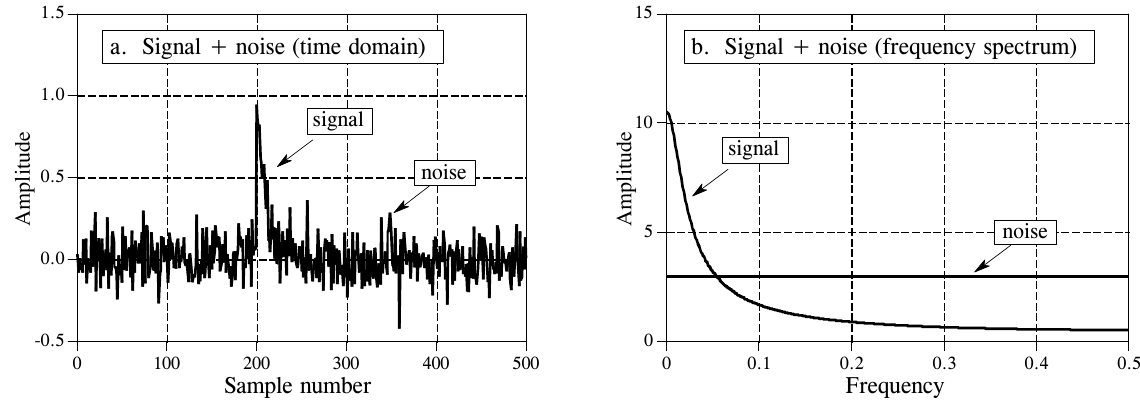
\includegraphics[width=0.950\linewidth,height=0.8\textheight,keepaspectratio]{assets/ch17/fig17-07.png}
\caption*{\textbf{图 17-7　最优滤波的例子。} (a)
是一个埋在随机噪声中的指数脉冲。脉冲和噪声的频谱如 (b)
所示。由于信号和噪声在时域和频域中都相互重叠，分离它们的最好办法并不显而易见。
（a. Signal + noise (time domain) = 信号 + 噪声（时域）；b. Signal +
noise (frequency spectrum) = 信号 + 噪声（频谱）；signal = 信号，noise =
噪声。Amplitude = 幅度，Sample number = 采样序号，Frequency = 频率。）}
\end{figure}

移动平均滤波器(moving average filter)是第 15
章的主题。你应该还记得，移动平均滤波器产生的每个输出点，都是输入信号中一定数量的点的平均值。这使得它的滤波器核是一个矩形脉冲，幅度等于参与平均的点数的倒数。移动平均滤波器的最优性在于：对于给定的降噪程度，它提供最快的阶跃响应。

匹配滤波器(matched filter)在第 7 章讨论过。如图 17-8a
所示，匹配滤波器的滤波器核与要检测的目标信号相同，只是做了左右翻转。匹配滤波器背后的思想是相关，而用卷积来实现相关需要这个翻转。输出信号中每个点的幅度，衡量的是滤波器核与输入信号相应片段的匹配程度。回想一下，匹配滤波器的输出不一定像被检测的信号。这其实无关紧要；如果用匹配滤波器，目标信号的形状肯定已经知道了。匹配滤波器的最优性在于：峰顶高出噪声的程度，比任何其他线性滤波器所能达到的都高（见图
17-9b）。

\begin{figure}[htbp]
\centering
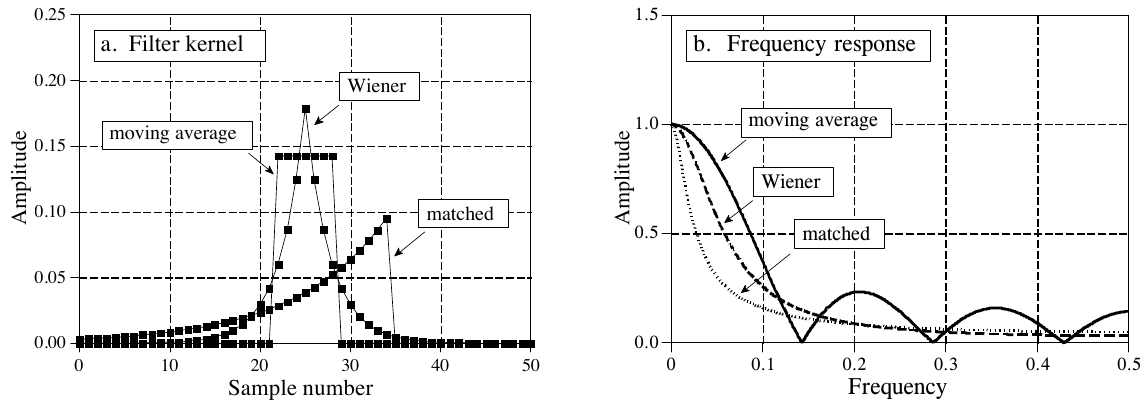
\includegraphics[width=0.954\linewidth,height=0.8\textheight,keepaspectratio]{assets/ch17/fig17-08.png}
\caption*{\textbf{图 17-8　最优滤波器的例子。} (a)
中画出了三个滤波器核，每一个都在某种意义上是最优的。相应的频率响应如 (b)
所示。移动平均滤波器被设计成以矩形脉冲为滤波器核。相比之下，匹配滤波器的核看起来像被检测的信号。维纳滤波器是在频域中设计的，依据的是每个频率上信号和噪声的相对多少。
（a. Filter kernel = 滤波器核；b. Frequency response = 频率响应；moving
average = 移动平均，Wiener = 维纳，matched = 匹配。Amplitude =
幅度，Sample number = 采样序号，Frequency = 频率。）}
\end{figure}

维纳滤波器(Wiener
filter，以诺伯特·维纳的最优估计理论命名)依据信号的频谱来分离信号。如图
17-7b
所示，在某些频率上主要是信号，在另一些频率上主要是噪声。看起来很合理的做法是：让''主要是信号''的频率通过滤波器，挡住''主要是噪声''的频率。维纳滤波器把这个思路又往前推了一步：滤波器在每个频率上的增益，由该频率上信号和噪声的相对多少决定：

\textbf{公式 17-1}　维纳滤波器。频率响应 H{[}f{]} 由噪声的频谱 N{[}f{]}
和信号的频谱 S{[}f{]} 决定。只有幅度起作用，所有相位都为零。

\[H[f] = \frac{S[f]^2}{S[f]^2 + N[f]^2}\]

用这个关系式，可以把图 17-7b 中的频谱转换成图 17-8b
中维纳滤波器的频率响应。维纳滤波器的最优性在于：它使信号功率与噪声功率之比最大（在整个信号长度上，而不是在每个单独的点上）。合适的滤波器核用自定义方法由维纳频率响应设计出来。

\begin{figure}[htbp]
\centering
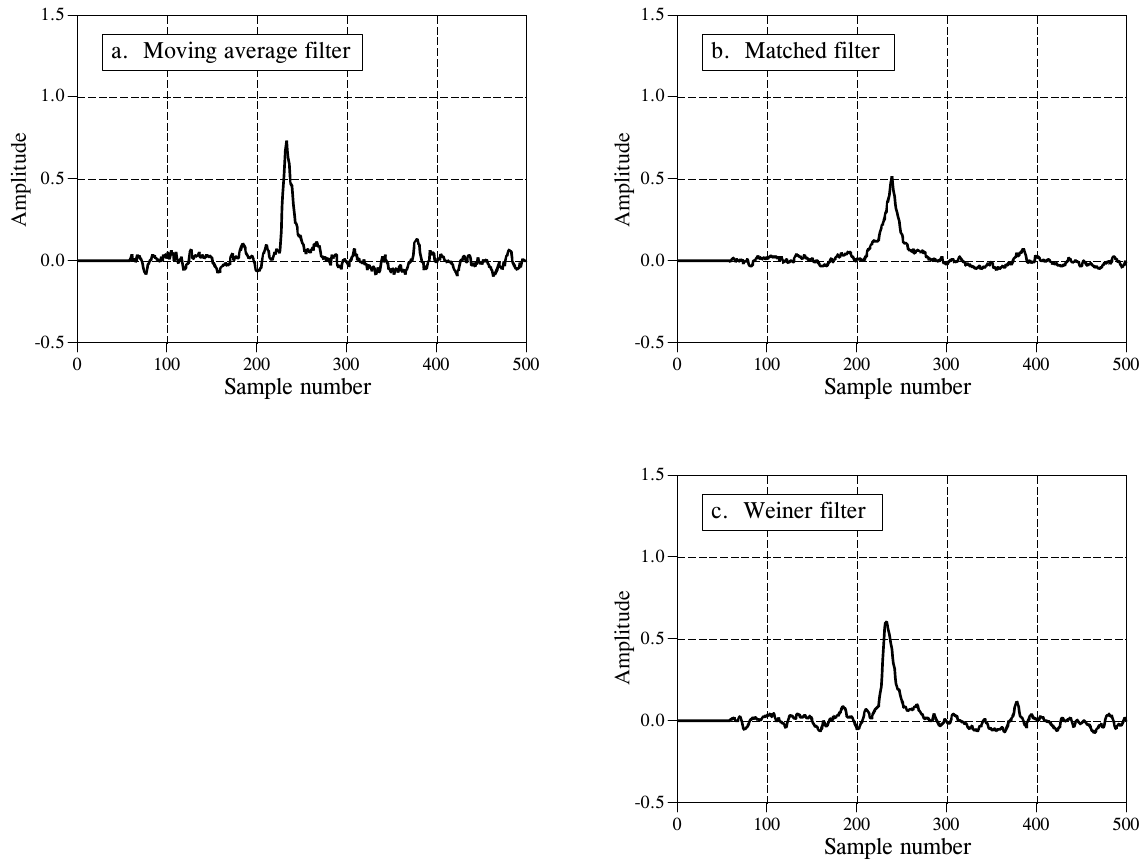
\includegraphics[width=0.950\linewidth,height=0.8\textheight,keepaspectratio]{assets/ch17/fig17-09.png}
\caption*{\textbf{图 17-9　使用三种最优滤波器的例子。} 这些信号是用图 17-8
中的滤波器对图 17-7
中的波形做滤波得到的。这三种滤波器都在某种意义上是最优的。(a)
中，对于给定的随机噪声降低程度，移动平均滤波器得到最陡峭的边缘响应。(b)
中，匹配滤波器产生的峰高出残余噪声的程度超过任何其他滤波器。(c)
中，维纳滤波器使信噪比最优。 （a. Moving average filter =
移动平均滤波器；b. Matched filter = 匹配滤波器；c.~Weiner filter =
维纳滤波器（原书把 Wiener 误拼成 Weiner）。Amplitude = 幅度，Sample
number = 采样序号。原书图注排在左下空白处，裁图时已去掉，译文见上。）}
\end{figure}

这些最优滤波器背后的思想在数学上很优雅，但在实践中常常不灵。这并不是说永远不该用它们。要点在于：别一听到''最优''二字就停止思考。我们来看几个你可能不想用它们的理由。

第一，图 17-9
中这几个信号之间的差别很不起眼。事实上，如果没人告诉你优化的是哪个参数，光看这些信号你大概分辨不出来。对于频谱重叠的问题，通常都是这样。最优滤波器带来的那一点额外性能，可能抵不上增加的程序复杂度、额外的设计工作量或更长的执行时间。

第二，维纳滤波器和匹配滤波器完全由问题本身的特性决定。其他滤波器，比如加窗
sinc
滤波器和移动平均滤波器，可以按你的喜好调整。最优滤波器的拥护者会说，这种摆弄只会降低滤波器的效果。这一点很值得商榷。记住，这些滤波器中的每一种都只在某一个特定的方面是最优的（即''在某种意义上''）。这很少足以说明整个问题都被优化了，尤其是当得到的信号要由人来解读的时候。例如，一位生物医学工程师可能用维纳滤波器来使心电图的信噪比最大。然而，这是否同时使医生通过看信号来发现心律异常的能力也达到最优，并不明显。

第三，维纳滤波器和匹配滤波器必须用卷积来实现，执行起来极慢。即使用下一章讨论的提速方法（FFT
卷积），计算时间也可能长得过分。相比之下，递归滤波器（比如移动平均滤波器或第
19 章介绍的其他滤波器）要快得多，而且可能提供可以接受的性能。

% !TEX root = ../main.tex
% 本文件由 build-tex.sh 从 18-DSP指南-第18章中译.md 生成，改内容请改 md 后重新生成

\chapter{FFT 卷积}\label{ch-18}

本章介绍两种重要的 DSP 技术：重叠相加法(overlap-add method)和 FFT
卷积(FFT convolution)。重叠相加法用来把长信号切成较短的段，以便处理。FFT
卷积把重叠相加法和快速傅里叶变换（Fast Fourier
Transform，FFT）结合起来，通过把两个信号的频谱相乘来完成卷积。对于长度超过大约
64 点的滤波器核，FFT 卷积比标准卷积更快，而结果完全相同。

\section{重叠相加法}

在许多 DSP 应用中，长信号必须分段滤波。例如，高保真数字音频的数据率约为
5 MB/分钟，数字视频约为 500
MB/分钟。数据率这么高，计算机的内存常常不够同时容纳要处理的整个信号。还有一些系统因为是实时运行的，只能一段一段地处理。例如，电话信号的延迟不能超过几百毫秒，这就限制了任何时刻能拿来处理的数据量。还有一些应用，是处理方法本身要求把信号分段。FFT
卷积就是一个例子，它也是本章的主题。

重叠相加法基于 DSP 的基本技巧：(1) 把信号分解成简单的分量；(2)
以某种有用的方式处理每个分量；(3) 把处理过的分量重新合成最终的信号。图
18-1 展示了重叠相加法怎样做到这一点。图 (a) 是要滤波的信号，(b)
是要用的滤波器核，一个窗函数 sinc 低通滤波器(windowed-sinc low-pass
filter)。跳到图的最下面，(i) 是滤波后的信号，是 (a)
的平滑版本。这种方法的关键在于卷积怎样影响这些信号的长度。一个 N
点信号与一个 M 点滤波器核卷积，输出信号长 N + M − 1 点。例如，输入信号
(a) 有 300 个采样（从 0 到 299），滤波器核 (b) 有 101 个采样（从 0 到
100），输出信号 (i) 有 400 个采样（从 0 到 399）。

换句话说，一个 N 点信号经过滤波后，会向右扩展 M − 1
个点。（这里假定滤波器核的下标从 0
开始。如果滤波器核用了负下标，信号也会向左扩展。）在 (a) 中，第 300 到
399 个采样处补上了零，用来表示扩展会发生在哪里。别被输出信号 (i)
两端那些很小的值迷惑了，这只是因为窗函数 sinc 滤波器核两端的值很小。(i)
中的全部 400 个采样都不为零，只是有些小到在图上看不出来。

图 (c)、(d)、(e)
展示了重叠相加法所用的分解。信号被切成若干段，每段包含原信号的 100
个采样。此外，每段右边再补上 100
个零。下一步，把每段分别与滤波器核卷积，单独滤波。这样就得到
(f)、(g)、(h) 所示的输出段。由于每个输入段长 100 个采样、滤波器核长 101
个采样，每个输出段将长 200 个采样。要理解的重点是：每个输入段补上 100
个零，就是为了给卷积时的扩展留出位置。

注意，扩展使得各输出段彼此重叠。把这些重叠的输出段相加，就得到输出信号
(i)。例如，(i) 中第 200 到 299 个采样，是把 (g) 和 (h)
中对应的采样相加得到的。重叠相加法得到的输出信号与直接卷积完全相同。缺点是程序要复杂得多，因为必须记录哪些采样是重叠的。

\begin{figure}[htbp]
\centering
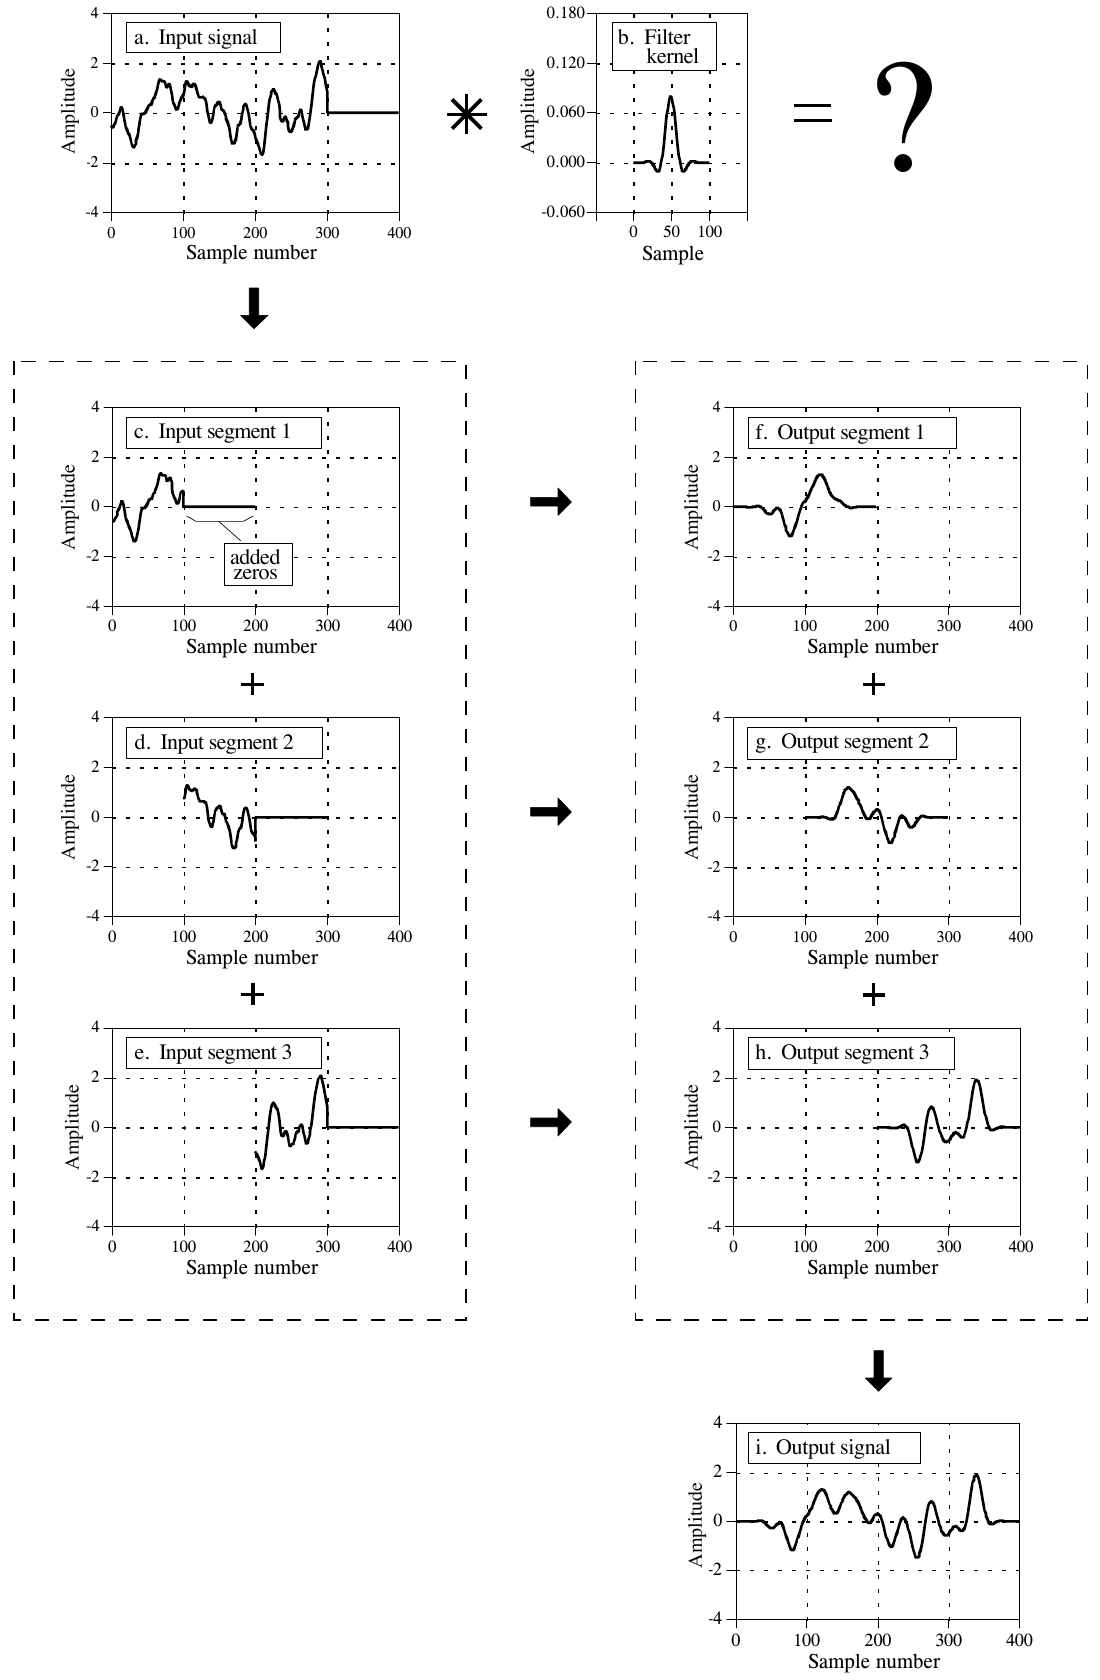
\includegraphics[width=0.917\linewidth,height=0.8\textheight,keepaspectratio]{assets/ch18/fig18-01.png}
\caption*{\textbf{图 18-1　重叠相加法。} 目标是把输入信号 (a) 与滤波器核 (b)
卷积。做法是把输入信号切成若干段，比如
(c)、(d)、(e)，每段补上足够多的零，为卷积时的扩展留出位置。把每个输入段与滤波器核卷积，得到输出段
(f)、(g)、(h)。再把这些重叠的输出段相加，就得到输出信号 (i)。 （a. Input
signal = 输入信号；b. Filter kernel = 滤波器核；c～e. Input segment 1～3
= 输入段 1～3，added zeros = 补上的零；f～h. Output segment 1～3 =
输出段 1～3；i. Output signal = 输出信号。Amplitude = 幅度，Sample
number / Sample = 采样序号。第一行的 \dspsym{∗} 是卷积。原书图注排在 (i)
的左边，裁图时已去掉，译文见上。）}
\end{figure}

\section{FFT 卷积}

FFT 卷积利用的原理是：频域中的乘法对应时域中的卷积。先用 DFT
把输入信号变换到频域，乘以滤波器的频率响应，再用逆 DFT
变换回时域。这个基本技术从傅里叶的年代就已为人所知，但当时没有人真正在意。原因是计算
DFT 所需的时间，比直接计算卷积的时间还长。1965
年快速傅里叶变换（FFT）的出现改变了这一点。用 FFT 算法来计算
DFT，经由频域的卷积就能比直接在时域卷积更快。最终结果是一样的，只是更高效的算法改变了计算量。因此，FFT
卷积也叫高速卷积(high-speed convolution)。

FFT 卷积使用图 18-1
所示的重叠相加法，改变的只是把输入段变成输出段的方式。图 18-2 展示了 FFT
卷积怎样把一个输入段变成一个输出段。首先，用 FFT 对滤波器核做
DFT，求出滤波器的频率响应。例如，(a) 是一个示例滤波器核，一个窗函数 sinc
带通滤波器(band-pass filter)。FFT 把它变成频率响应的实部和虚部，见 (b)
和
(c)。这些频域信号可能看起来不像带通滤波器，因为它们是直角坐标形式。记住，人理解频域通常用极坐标形式最好，而数学计算通常用直角坐标形式最好。这些实部和虚部存放在计算机里，留待计算每一段时使用。

图 (d) 是正在处理的输入段。用 FFT 求出它的频谱，见 (e) 和
(f)。然后把滤波器的频率响应 (b)、(c) 乘以输入段的频谱
(e)、(f)，得到输出段的频谱
(h)、(i)。由于这些频谱由实部和虚部组成，要按第 9 章的公式 9-1
相乘。再用逆 FFT 从频谱 (h)、(i) 求出输出段
(g)。重要的是要认识到，这个输出段与把输入段 (d) 和滤波器核 (a)
直接卷积得到的结果完全相同。

FFT 必须足够长，才不会发生循环卷积(circular convolution)（第 9
章也讲过）。这意味着 FFT 的长度应当与输出段 (g) 的长度相同。例如，在图
18-2 的例子中，滤波器核有 129 点，每段有 128 点，所以输出段长 256
点。这就要求使用 256 点 FFT。也就是说，滤波器核 (a) 必须补上 127
个零，使总长度达到 256 点。同样，每个输入段 (d) 必须补上 128
个零。再举一个例子，设想你要把一个很长的信号与一个 600
点的滤波器核卷积。一种选择是每段 425 点、用 1024 点
FFT；另一种选择是每段 1449 点、用 2048 点 FFT。

\begin{figure}[htbp]
\centering
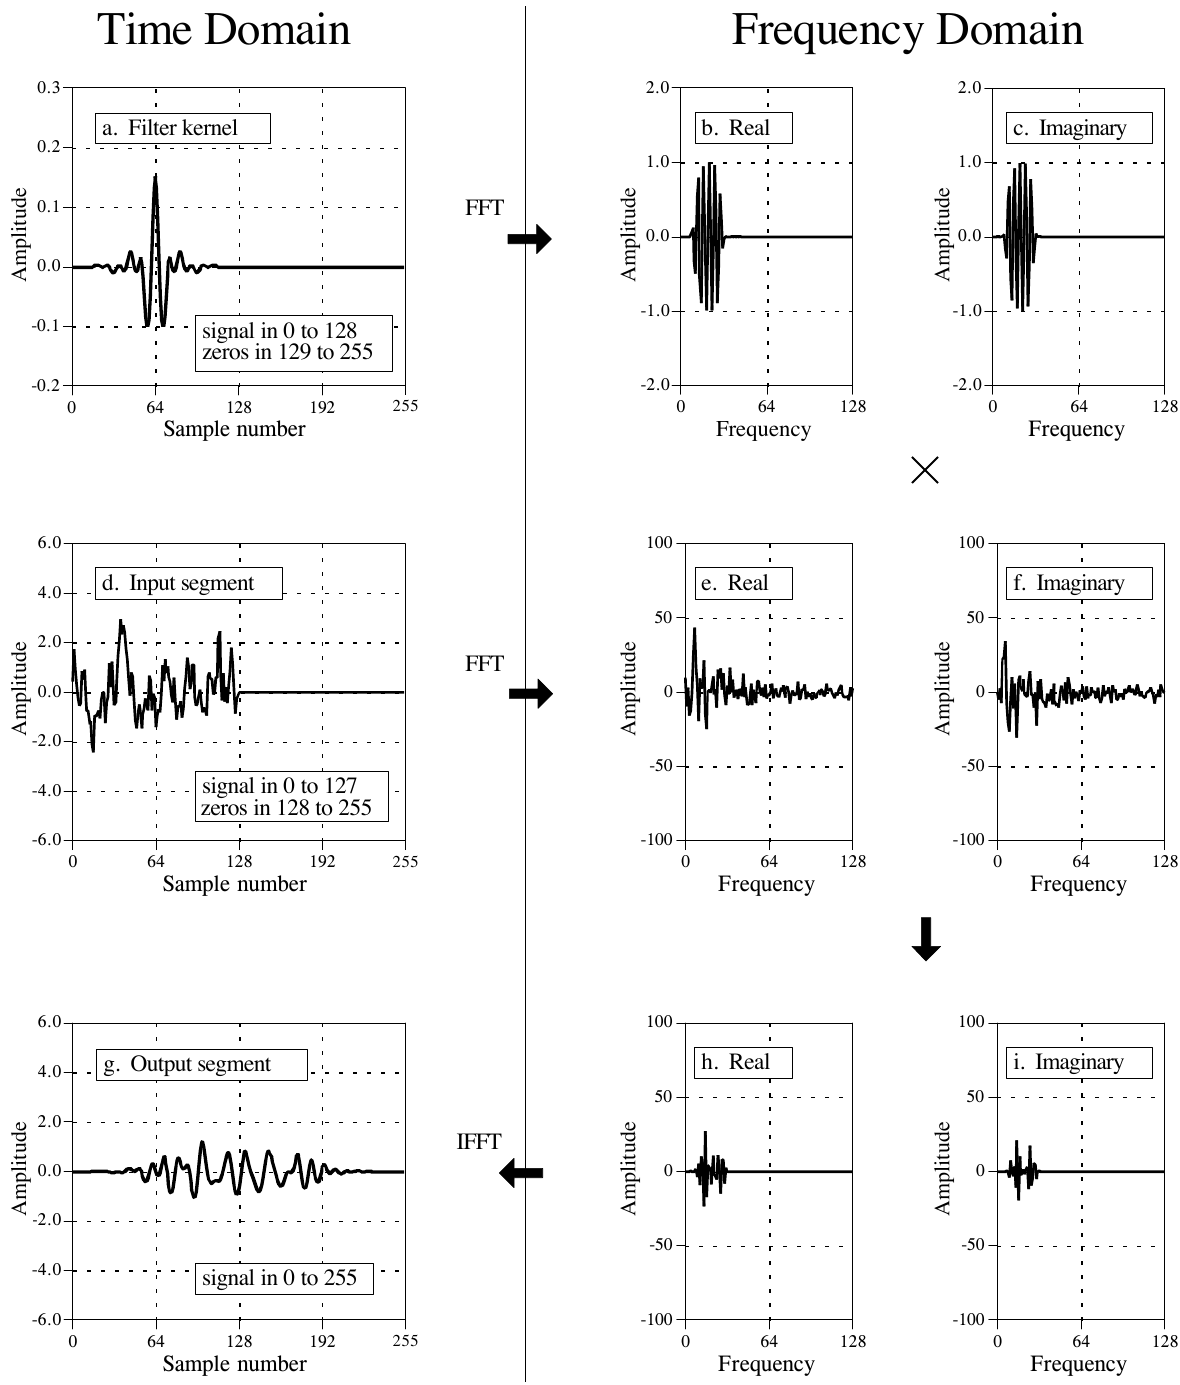
\includegraphics[width=0.983\linewidth,height=0.8\textheight,keepaspectratio]{assets/ch18/fig18-02.png}
\caption*{\textbf{图 18-2　FFT 卷积。} 滤波器核 (a) 和信号段 (d) 经 FFT
分别变成各自的频谱 (b)、(c) 和
(e)、(f)。这两个频谱相乘，得到输出段的频谱 (h)、(i)。再由逆 FFT
求出输出段 (g)。 （Time Domain = 时域，Frequency Domain = 频域；a.
Filter kernel = 滤波器核，signal in 0 to 128, zeros in 129 to 255 = 第
0～128 点是信号，第 129～255 点是零；b/e/h. Real = 实部；c/f/i.
Imaginary = 虚部；d.~Input segment = 输入段，signal in 0 to 127, zeros
in 128 to 255 = 第 0～127 点是信号，第 128～255 点是零；g. Output
segment = 输出段，signal in 0 to 255 = 第 0～255 点都是信号。FFT
箭头表示正变换，IFFT 表示逆变换，× 表示两个频谱相乘。Amplitude =
幅度，Sample number = 采样序号，Frequency =
频率。原书图注把输入段的频谱写成 ``(d) \& (e)''，应为 (e) 和
(f)，译文已改正。）}
\end{figure}

表 18-1 是一个执行 FFT 卷积的示例程序。这个程序把一个 1000
万点的信号与一个 400 点的滤波器核卷积。做法是把输入信号切成 16000
段，每段 625 点。每段与滤波器核卷积，得到一个 625 + 400 − 1 = 1024
点的输出段。因此使用 1024 点 FFT。在定义并初始化所有数组之后（第
130～230 行），第一步是计算并保存滤波器的频率响应（第 250～310 行）。第
260 行调用一个虚构的子程序，把滤波器核载入 XX{[}0{]} 到
XX{[}399{]}，并把 XX{[}400{]} 到 XX{[}1023{]} 设为零。第 270
行的子程序是 FFT，把 XX{[} {]} 中的 1024 个采样变换成 REX{[} {]} 和
IMX{[} {]} 中的 513 个采样，即频率响应的实部和虚部。这些值被转存到数组
REFR{[} {]} 和 IMFR{[} {]} 中（意为 REal and IMaginary Frequency
Response，频率响应的实部和虚部），供程序后面使用。

第 340 到 580 行之间的 FOR-NEXT 循环控制 16000 段的处理。在第 360
行，一个子程序把下一段要处理的数据载入 XX{[}0{]} 到 XX{[}624{]}，并把
XX{[}625{]} 到 XX{[}1023{]} 设为零。在第 370 行，用 FFT
子程序求出这一段的频谱，实部放进 REX{[} {]} 的 513 个点，虚部放进 IMX{[}
{]} 的 513 个点。第 390～430 行是把这一段的频谱（存放在 REX{[} {]} 和
IMX{[} {]}）乘以滤波器的频率响应（存放在 REFR{[} {]} 和 IMFR{[}
{]}）。相乘的结果存回 REX{[} {]} 和 IMX{[}
{]}，覆盖原来的数据。由于这时它已经是输出段的频谱，就可以用 IFFT
求出输出段。这由第 450 行虚构的 IFFT 子程序完成，它把 REX{[} {]} 和
IMX{[} {]} 中的 513 个点变换成 XX{[} {]} 中的 1024 个点，即输出段。

第 470～550 行处理段与段之间的重叠。每个输出段分为两部分。前 625 个点（0
到 624）需要与上一个输出段的重叠部分相加，然后写入输出信号。后 399
个点（625 到 1023）需要保存起来，以便与下一个输出段重叠。

要理解这一点，回头看图 18-1。(g) 中第 100 到 199
个采样需要与上一个输出段 (f) 的重叠部分相加，然后就可以移到输出信号 (i)
中。相比之下，(g) 中第 200 到 299 个采样需要保存起来，以便与下一个输出段
(h) 相加。

现在回到程序。数组 OLAP{[} {]} 用来存放从一段重叠到下一段的 399
个采样。在第 470～490 行，把这个数组中（来自上一个输出段）的 399
个值加到当前正在处理的输出段上，该输出段存放在 XX{[} {]} 中。然后第 550
行的虚构子程序把 XX{[}0{]} 到 XX{[}624{]} 中的 625
个采样输出到存放输出信号的文件。当前输出段中需要留给下一个输出段的 399
个采样，在第 510～530 行存入 OLAP{[} {]}。

第 0 到 15999 段全部处理完后，数组 OLAP{[} {]} 中存放的是第 15999
段中应当与第 16000 段重叠的 399 个采样。由于第 16000
段并不存在（或者可以看作全是零），这 399 个采样在第 600
行直接写入输出信号。这使得输出信号的长度为 16000 × 625 + 399 =
10,000,399 点。这正好等于输入信号的长度加上滤波器核的长度再减一。

\textbf{表 18-1}（注释已译成中文）

\begin{Shaded}
\begin{Highlighting}[]
\NormalTok{100 \textquotesingle{}FFT 卷积}
\NormalTok{110 \textquotesingle{}本程序把一个 1000 万点的信号与一个 400 点的滤波器核卷积。输入}
\NormalTok{120 \textquotesingle{}信号切成 16000 段，每段 625 点。使用 1024 点 FFT。}
\NormalTok{130 \textquotesingle{}}
\NormalTok{130 \textquotesingle{}                                \textquotesingle{}初始化各数组}
\NormalTok{140 DIM XX[1023]                     \textquotesingle{}时域信号（供 FFT 使用）}
\NormalTok{150 DIM REX[512]                     \textquotesingle{}频域的实部（供 FFT 使用）}
\NormalTok{160 DIM IMX[512]                     \textquotesingle{}频域的虚部（供 FFT 使用）}
\NormalTok{170 DIM REFR[512]                    \textquotesingle{}滤波器频率响应的实部}
\NormalTok{180 DIM IMFR[512]                    \textquotesingle{}滤波器频率响应的虚部}
\NormalTok{190 DIM OLAP[398]                    \textquotesingle{}存放段与段之间重叠的采样}
\NormalTok{200 \textquotesingle{}}
\NormalTok{210 FOR I\% = 0 TO 398                \textquotesingle{}把存放重叠采样的数组清零}
\NormalTok{220 OLAP[I\%] = 0}
\NormalTok{230 NEXT I\%}
\NormalTok{240 \textquotesingle{}}
\NormalTok{250 \textquotesingle{}                                \textquotesingle{}求出并保存滤波器的频率响应}
\NormalTok{260 GOSUB XXXX                       \textquotesingle{}虚构的子程序，把滤波器核载入 XX[ ]}
\NormalTok{270 GOSUB XXXX                       \textquotesingle{}虚构的 FFT 子程序：XX[ ] {-}{-}\textgreater{} REX[ ] \& IMX[ ]}
\NormalTok{280 FOR F\% = 0 TO 512                \textquotesingle{}把频率响应存入 REFR[ ] 和 IMFR[ ]}
\NormalTok{290 REFR[F\%] = REX[F\%]}
\NormalTok{300 IMFR[F\%] = IMX[F\%]}
\NormalTok{310 NEXT F\%}
\NormalTok{320 \textquotesingle{}}
\NormalTok{330 \textquotesingle{}                                \textquotesingle{}逐个处理 16000 段}
\NormalTok{340 FOR SEGMENT\% = 0 TO 15999}
\NormalTok{350 \textquotesingle{}}
\NormalTok{360 GOSUB XXXX                       \textquotesingle{}虚构的子程序，把下一个输入段载入 XX[ ]}
\NormalTok{370 GOSUB XXXX                       \textquotesingle{}虚构的 FFT 子程序：XX[ ] {-}{-}\textgreater{} REX[ ] \& IMX[ ]}
\NormalTok{380 \textquotesingle{}}
\NormalTok{390 FOR F\% = 0 TO 512                \textquotesingle{}频谱乘以频率响应}
\NormalTok{400 TEMP    = REX[F\%]*REFR[F\%] {-} IMX[F\%]*IMFR[F\%]}
\NormalTok{410 IMX[F\%] = REX[F\%]*IMFR[F\%] + IMX[F\%]*REFR[F\%]}
\NormalTok{420 REX[F\%] = TEMP}
\NormalTok{430 NEXT F\%}
\NormalTok{440 \textquotesingle{}}
\NormalTok{450 GOSUB XXXX                       \textquotesingle{}虚构的 IFFT 子程序：REX[ ] \& IMX[ ] {-}{-}\textgreater{} XX[ ]}
\NormalTok{460 \textquotesingle{}}
\NormalTok{470 FOR I\% = 0 TO 398                \textquotesingle{}把上一段的重叠部分加到这一段上}
\NormalTok{480 XX[I\%] = XX[I\%] + OLAP[I\%]}
\NormalTok{490 NEXT I\%}
\NormalTok{500 \textquotesingle{}}
\NormalTok{510 FOR I\% = 625 TO 1023             \textquotesingle{}保存要与下一段重叠的采样}
\NormalTok{520 OLAP[I\%{-}625] = XX[I\%]}
\NormalTok{530 NEXT I\%}
\NormalTok{540 \textquotesingle{}}
\NormalTok{550 GOSUB XXXX                       \textquotesingle{}虚构的子程序，输出存放在}
\NormalTok{560 \textquotesingle{}                                \textquotesingle{}XX[0] 到 XX[624] 中的 625 个采样}
\NormalTok{570 \textquotesingle{}}
\NormalTok{580 NEXT SEGMENT\%}
\NormalTok{590 \textquotesingle{}}
\NormalTok{600 GOSUB XXXX                       \textquotesingle{}虚构的子程序，输出 OLAP[ ] 中的全部 399 个采样}
\NormalTok{610 END}
\end{Highlighting}
\end{Shaded}

\begin{quote}
\textbf{译注：} 原书第 130 行重复出现了两次，是排版错误，不影响理解。
\end{quote}

\textbf{C 实现}（完整可编译版本见
\texttt{c/table18-1\_fft\_convolution.c}。原书的 FFT、IFFT
和数据读写都是''虚构的子程序''，这里 FFT 用表 12-4 的复数 FFT，逆 FFT
用表 12-5 的共轭法；为了能和直接卷积逐点对比，默认只处理 160
段，段数可用命令行参数修改）：

\begin{Shaded}
\begin{Highlighting}[]
\PreprocessorTok{\#define NFFT }\DecValTok{1024}\PreprocessorTok{                           }\CommentTok{/* 140 DIM XX[1023]：FFT 长度 */}
\PreprocessorTok{\#define NSEG }\DecValTok{625}\PreprocessorTok{                            }\CommentTok{/* 每段输入的点数 */}
\PreprocessorTok{\#define NK   }\DecValTok{400}\PreprocessorTok{                            }\CommentTok{/* 滤波器核的点数 */}
\PreprocessorTok{\#define NOL  }\OperatorTok{(}\PreprocessorTok{NK }\OperatorTok{{-}}\PreprocessorTok{ }\DecValTok{1}\OperatorTok{)}\PreprocessorTok{                       }\CommentTok{/* 190 DIM OLAP[398]：段与段之间重叠的 399 点 */}

\CommentTok{/* FFT 卷积主体，对应原书第 210～600 行。x 长 nseg*NSEG，y 长 nseg*NSEG + NOL */}
\DataTypeTok{static} \DataTypeTok{void}\NormalTok{ fft\_convolve}\OperatorTok{(}\DataTypeTok{const} \DataTypeTok{double} \OperatorTok{*}\NormalTok{x}\OperatorTok{,} \DataTypeTok{const} \DataTypeTok{double} \OperatorTok{*}\NormalTok{h}\OperatorTok{,} \DataTypeTok{int}\NormalTok{ nseg}\OperatorTok{,} \DataTypeTok{double} \OperatorTok{*}\NormalTok{y}\OperatorTok{)}
\OperatorTok{\{}
    \DataTypeTok{static} \DataTypeTok{double}\NormalTok{ xx}\OperatorTok{[}\NormalTok{NFFT}\OperatorTok{],}\NormalTok{ imx}\OperatorTok{[}\NormalTok{NFFT}\OperatorTok{];}          \CommentTok{/* 140～160：XX[ ]、REX[ ]（与 XX 共用）、IMX[ ] */}
    \DataTypeTok{static} \DataTypeTok{double}\NormalTok{ refr}\OperatorTok{[}\NormalTok{NFFT}\OperatorTok{],}\NormalTok{ imfr}\OperatorTok{[}\NormalTok{NFFT}\OperatorTok{];}       \CommentTok{/* 170～180：滤波器的频率响应 */}
    \DataTypeTok{double}\NormalTok{ olap}\OperatorTok{[}\NormalTok{NOL}\OperatorTok{];}                           \CommentTok{/* 190 */}

    \ControlFlowTok{for} \OperatorTok{(}\DataTypeTok{int}\NormalTok{ i }\OperatorTok{=} \DecValTok{0}\OperatorTok{;}\NormalTok{ i }\OperatorTok{\textless{}}\NormalTok{ NOL}\OperatorTok{;}\NormalTok{ i}\OperatorTok{++)}\NormalTok{ olap}\OperatorTok{[}\NormalTok{i}\OperatorTok{]} \OperatorTok{=} \DecValTok{0}\OperatorTok{;}  \CommentTok{/* 210～230：重叠数组清零 */}

    \ControlFlowTok{for} \OperatorTok{(}\DataTypeTok{int}\NormalTok{ i }\OperatorTok{=} \DecValTok{0}\OperatorTok{;}\NormalTok{ i }\OperatorTok{\textless{}}\NormalTok{ NFFT}\OperatorTok{;}\NormalTok{ i}\OperatorTok{++)} \OperatorTok{\{}            \CommentTok{/* 260：核放进 XX[0]～XX[399]，其余补零 */}
\NormalTok{        refr}\OperatorTok{[}\NormalTok{i}\OperatorTok{]} \OperatorTok{=}\NormalTok{ i }\OperatorTok{\textless{}}\NormalTok{ NK }\OperatorTok{?}\NormalTok{ h}\OperatorTok{[}\NormalTok{i}\OperatorTok{]} \OperatorTok{:} \FloatTok{0.0}\OperatorTok{;}
\NormalTok{        imfr}\OperatorTok{[}\NormalTok{i}\OperatorTok{]} \OperatorTok{=} \FloatTok{0.0}\OperatorTok{;}
    \OperatorTok{\}}
\NormalTok{    fft}\OperatorTok{(}\NormalTok{refr}\OperatorTok{,}\NormalTok{ imfr}\OperatorTok{,}\NormalTok{ NFFT}\OperatorTok{);}                      \CommentTok{/* 270～310：求出并保存滤波器的频率响应 */}

    \ControlFlowTok{for} \OperatorTok{(}\DataTypeTok{int}\NormalTok{ seg }\OperatorTok{=} \DecValTok{0}\OperatorTok{;}\NormalTok{ seg }\OperatorTok{\textless{}}\NormalTok{ nseg}\OperatorTok{;}\NormalTok{ seg}\OperatorTok{++)} \OperatorTok{\{}      \CommentTok{/* 340：逐段处理 */}
        \ControlFlowTok{for} \OperatorTok{(}\DataTypeTok{int}\NormalTok{ i }\OperatorTok{=} \DecValTok{0}\OperatorTok{;}\NormalTok{ i }\OperatorTok{\textless{}}\NormalTok{ NFFT}\OperatorTok{;}\NormalTok{ i}\OperatorTok{++)} \OperatorTok{\{}        \CommentTok{/* 360：本段放进 XX[0]～XX[624]，其余补零 */}
\NormalTok{            xx}\OperatorTok{[}\NormalTok{i}\OperatorTok{]} \OperatorTok{=}\NormalTok{ i }\OperatorTok{\textless{}}\NormalTok{ NSEG }\OperatorTok{?}\NormalTok{ x}\OperatorTok{[}\NormalTok{seg }\OperatorTok{*}\NormalTok{ NSEG }\OperatorTok{+}\NormalTok{ i}\OperatorTok{]} \OperatorTok{:} \FloatTok{0.0}\OperatorTok{;}
\NormalTok{            imx}\OperatorTok{[}\NormalTok{i}\OperatorTok{]} \OperatorTok{=} \FloatTok{0.0}\OperatorTok{;}
        \OperatorTok{\}}
\NormalTok{        fft}\OperatorTok{(}\NormalTok{xx}\OperatorTok{,}\NormalTok{ imx}\OperatorTok{,}\NormalTok{ NFFT}\OperatorTok{);}                     \CommentTok{/* 370：本段的频谱 */}

        \ControlFlowTok{for} \OperatorTok{(}\DataTypeTok{int}\NormalTok{ f }\OperatorTok{=} \DecValTok{0}\OperatorTok{;}\NormalTok{ f }\OperatorTok{\textless{}}\NormalTok{ NFFT}\OperatorTok{;}\NormalTok{ f}\OperatorTok{++)} \OperatorTok{\{}        \CommentTok{/* 390～430：频谱乘以频率响应（复数乘法，公式 9{-}1） */}
            \DataTypeTok{double}\NormalTok{ temp }\OperatorTok{=}\NormalTok{ xx}\OperatorTok{[}\NormalTok{f}\OperatorTok{]} \OperatorTok{*}\NormalTok{ refr}\OperatorTok{[}\NormalTok{f}\OperatorTok{]} \OperatorTok{{-}}\NormalTok{ imx}\OperatorTok{[}\NormalTok{f}\OperatorTok{]} \OperatorTok{*}\NormalTok{ imfr}\OperatorTok{[}\NormalTok{f}\OperatorTok{];}
\NormalTok{            imx}\OperatorTok{[}\NormalTok{f}\OperatorTok{]} \OperatorTok{=}\NormalTok{ xx}\OperatorTok{[}\NormalTok{f}\OperatorTok{]} \OperatorTok{*}\NormalTok{ imfr}\OperatorTok{[}\NormalTok{f}\OperatorTok{]} \OperatorTok{+}\NormalTok{ imx}\OperatorTok{[}\NormalTok{f}\OperatorTok{]} \OperatorTok{*}\NormalTok{ refr}\OperatorTok{[}\NormalTok{f}\OperatorTok{];}
\NormalTok{            xx}\OperatorTok{[}\NormalTok{f}\OperatorTok{]} \OperatorTok{=}\NormalTok{ temp}\OperatorTok{;}                       \CommentTok{/* 原书只乘 0～512 点（实数 FFT 的输出），这里用复数 FFT，0～1023 全乘 */}
        \OperatorTok{\}}

\NormalTok{        inverse\_fft}\OperatorTok{(}\NormalTok{xx}\OperatorTok{,}\NormalTok{ imx}\OperatorTok{,}\NormalTok{ NFFT}\OperatorTok{);}             \CommentTok{/* 450：回到时域，得到 1024 点输出段 */}

        \ControlFlowTok{for} \OperatorTok{(}\DataTypeTok{int}\NormalTok{ i }\OperatorTok{=} \DecValTok{0}\OperatorTok{;}\NormalTok{ i }\OperatorTok{\textless{}}\NormalTok{ NOL}\OperatorTok{;}\NormalTok{ i}\OperatorTok{++)}           \CommentTok{/* 470～490：加上上一段留下的重叠部分 */}
\NormalTok{            xx}\OperatorTok{[}\NormalTok{i}\OperatorTok{]} \OperatorTok{+=}\NormalTok{ olap}\OperatorTok{[}\NormalTok{i}\OperatorTok{];}
        \ControlFlowTok{for} \OperatorTok{(}\DataTypeTok{int}\NormalTok{ i }\OperatorTok{=}\NormalTok{ NSEG}\OperatorTok{;}\NormalTok{ i }\OperatorTok{\textless{}}\NormalTok{ NFFT}\OperatorTok{;}\NormalTok{ i}\OperatorTok{++)}       \CommentTok{/* 510～530：保存要和下一段重叠的 399 点 */}
\NormalTok{            olap}\OperatorTok{[}\NormalTok{i }\OperatorTok{{-}}\NormalTok{ NSEG}\OperatorTok{]} \OperatorTok{=}\NormalTok{ xx}\OperatorTok{[}\NormalTok{i}\OperatorTok{];}
        \ControlFlowTok{for} \OperatorTok{(}\DataTypeTok{int}\NormalTok{ i }\OperatorTok{=} \DecValTok{0}\OperatorTok{;}\NormalTok{ i }\OperatorTok{\textless{}}\NormalTok{ NSEG}\OperatorTok{;}\NormalTok{ i}\OperatorTok{++)}          \CommentTok{/* 550：输出 XX[0]～XX[624] */}
\NormalTok{            y}\OperatorTok{[}\NormalTok{seg }\OperatorTok{*}\NormalTok{ NSEG }\OperatorTok{+}\NormalTok{ i}\OperatorTok{]} \OperatorTok{=}\NormalTok{ xx}\OperatorTok{[}\NormalTok{i}\OperatorTok{];}
    \OperatorTok{\}}
    \ControlFlowTok{for} \OperatorTok{(}\DataTypeTok{int}\NormalTok{ i }\OperatorTok{=} \DecValTok{0}\OperatorTok{;}\NormalTok{ i }\OperatorTok{\textless{}}\NormalTok{ NOL}\OperatorTok{;}\NormalTok{ i}\OperatorTok{++)}               \CommentTok{/* 600：最后一段的重叠部分直接输出 */}
\NormalTok{        y}\OperatorTok{[}\NormalTok{nseg }\OperatorTok{*}\NormalTok{ NSEG }\OperatorTok{+}\NormalTok{ i}\OperatorTok{]} \OperatorTok{=}\NormalTok{ olap}\OperatorTok{[}\NormalTok{i}\OperatorTok{];}
\OperatorTok{\}}
\end{Highlighting}
\end{Shaded}

运行结果（随机输入信号、400 点窗函数 sinc 低通核）：

{\def\LTcaptype{none} % do not increment counter
\begin{longtable}[]{@{}
  >{\raggedright\arraybackslash}p{(\linewidth - 8\tabcolsep) * \real{0.2000}}
  >{\raggedright\arraybackslash}p{(\linewidth - 8\tabcolsep) * \real{0.2000}}
  >{\raggedright\arraybackslash}p{(\linewidth - 8\tabcolsep) * \real{0.2000}}
  >{\raggedright\arraybackslash}p{(\linewidth - 8\tabcolsep) * \real{0.2000}}
  >{\raggedright\arraybackslash}p{(\linewidth - 8\tabcolsep) * \real{0.2000}}@{}}
\toprule\noalign{}
\begin{minipage}[b]{\linewidth}\raggedright
输入
\end{minipage} & \begin{minipage}[b]{\linewidth}\raggedright
输出长度
\end{minipage} & \begin{minipage}[b]{\linewidth}\raggedright
与直接卷积的最大偏差
\end{minipage} & \begin{minipage}[b]{\linewidth}\raggedright
FFT 卷积耗时
\end{minipage} & \begin{minipage}[b]{\linewidth}\raggedright
直接卷积耗时
\end{minipage} \\
\midrule\noalign{}
\endhead
\bottomrule\noalign{}
\endlastfoot
160 段 × 625 = 10 万点 & 100,399 点 & 1.7e-14 & 2.2 ms & 32.7 ms \\
1600 段 × 625 = 100 万点 & 1,000,399 点 & 2.0e-14 & 21.9 ms & 320.1
ms \\
\end{longtable}
}

两种方法的输出逐点一致（偏差只是双精度舍入误差），输出长度也都等于''输入长度
+ 核长度 − 1''。对于 400 点的核，FFT 卷积约快 15 倍。

\section{速度的提升}

FFT 卷积什么时候比标准卷积快？答案取决于滤波器核的长度，如图 18-3
所示。标准卷积所需的时间与滤波器核的点数成正比。相比之下，FFT
卷积所需的时间增长得非常慢，只与滤波器核点数的对数成正比。两者的交叉点出现在滤波器核约有
40 到 80 个采样时（取决于所用的具体硬件）。

\begin{figure}[htbp]
\centering
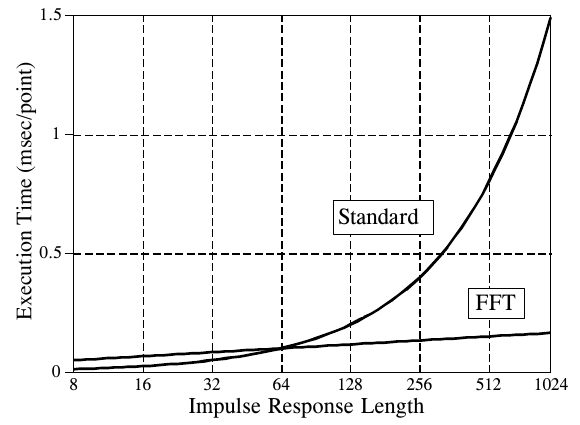
\includegraphics[width=0.483\linewidth,height=0.8\textheight,keepaspectratio]{assets/ch18/fig18-03.png}
\caption*{\textbf{图 18-3　FFT 卷积的执行时间。} 当滤波器核长于约 60 点时，FFT
卷积比标准方法快。这些执行时间是在 100 MHz
奔腾上、使用单精度浮点数测得的。 （Execution Time (msec/point) =
执行时间（毫秒/点），Impulse Response Length = 冲激响应长度；Standard =
标准卷积，FFT = FFT
卷积。原书图注排在图的左边，裁图时已去掉，译文见上。）}
\end{figure}

要记住的要点是：短于约 60
点的滤波器核用标准卷积实现更快，执行时间与核的长度成正比。更长的滤波器核用
FFT 卷积实现更快。用 FFT
卷积时，滤波器核想做多长都可以，执行时间几乎不受影响。例如，一个 16,000
点的滤波器核，执行时间只比 64 点的核长大约一倍。

卷积的速度也决定了计算的精度（就像第 12 章讲 FFT
时说的那样）。这是因为输出信号中的舍入误差取决于计算的总次数，而计算次数与计算时间成正比。输出信号算得越快，也就算得越精确。例如，设想用单精度浮点数把一个信号与一个
1000
点的滤波器核卷积。用标准卷积，典型的舍入噪声预计约为两万分之一（根据第 4
章的经验法则）。相比之下，FFT
卷积预计会快一个数量级，精度也高一个数量级（即二十万分之一）。

把 FFT
卷积收好，留到你有大量数据要处理、又需要极长的滤波器核时再用。想想一百万个采样的信号和一千点的滤波器核这样的规模。达不到这个规模，就不值得多花这些编程功夫。不想自己写
FFT
卷积程序？去软件库和软件包里找现成的代码。可以先从本书的网站找起（见版权页）。

% !TEX root = ../main.tex
% 本文件由 build-tex.sh 从 19-DSP指南-第19章中译.md 生成，改内容请改 md 后重新生成

\chapter{递归滤波器}\label{ch-19}

递归滤波器(recursive
filter)是一种不必做很长的卷积、就能得到很长冲激响应的高效方法。它们执行起来非常快，但性能和灵活性不如其他数字滤波器。递归滤波器也叫无限冲激响应(Infinite
Impulse
Response，IIR)滤波器，因为它们的冲激响应由衰减的指数函数组成。这把它们和用卷积实现的数字滤波器区分开来，后者叫有限冲激响应(Finite
Impulse
Response，FIR)滤波器。本章介绍递归滤波器怎样工作，以及怎样设计这个家族中的简单成员。第
20、26 和 33 章会介绍更精巧的设计方法。

\section{递归方法}

为了开始讨论递归滤波器，设想你需要从某个信号 x{[} {]}
中提取信息。你的需求如此迫切，以至于雇了一位老数学教授来替你处理数据。教授的任务是对
x{[} {]} 滤波，得到 y{[} {]}，你希望 y{[} {]}
里包含你感兴趣的信息。教授开始工作，按照锁在他过度发达的大脑里的某种算法，逐点计算
y{[}
{]}。做到一半，发生了一件极其不幸的事：教授开始念叨解析奇点、分数阶变换，以及数学家噩梦里的其他妖魔鬼怪。很明显，教授疯了。你焦急地看着教授------连同你的算法------被几个穿白大褂的人带走了。

你发疯似地翻阅教授的笔记，想找出他用的算法。你发现他已经算完了 y{[}0{]}
到 y{[}27{]}，正要开始算 y{[}28{]}。如图 19-1 所示，我们用变量 n
表示当前正在计算的点。这意味着 y{[}n{]} 是输出信号的第 28
个采样，y{[}n−1{]} 是第 27 个，y{[}n−2{]} 是第 26
个，依此类推。同样，x{[}n{]} 是输入信号的第 28 个点，x{[}n−1{]} 是第 27
个点，依此类推。为了理解所用的算法，我们问自己：``教授在计算正在处理的采样
y{[}n{]} 时，手头有哪些信息？''

\begin{figure}[htbp]
\centering
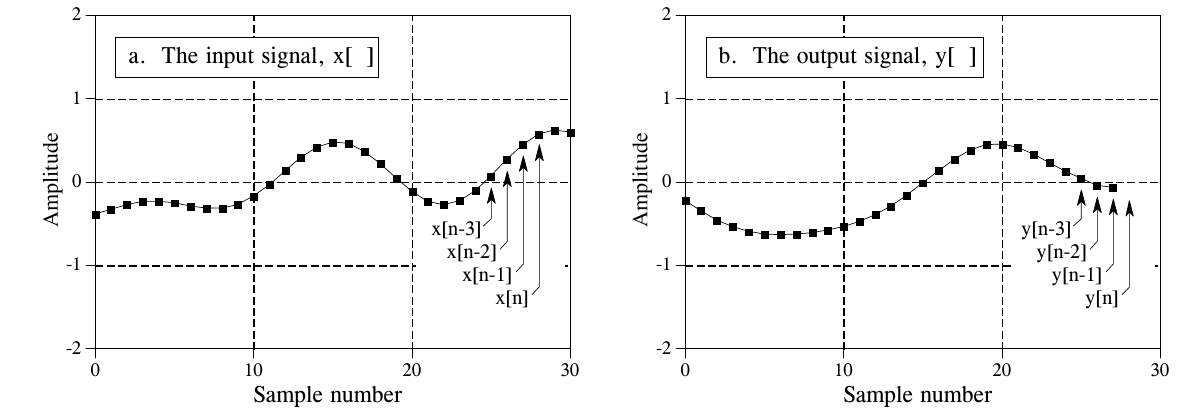
\includegraphics[width=0.988\linewidth,height=0.8\textheight,keepaspectratio]{assets/ch19/fig19-01.png}
\caption*{\textbf{图 19-1　递归滤波器的记法。} 正在计算的输出采样
y{[}n{]}，由输入信号的值
x{[}n{]}、x{[}n−1{]}、x{[}n−2{]}、\dspsym{⋯}，以及输出信号中先前已算出的值
y{[}n−1{]}、y{[}n−2{]}、y{[}n−3{]}、\dspsym{⋯} 决定。图中 n = 28。 （a.
The input signal, x{[} {]} = 输入信号 x{[} {]}；b. The output signal,
y{[} {]} = 输出信号 y{[} {]}。Amplitude = 幅度，Sample number =
采样序号。）}
\end{figure}

最明显的信息来源是输入信号，即这些值：x{[}n{]}、x{[}n−1{]}、x{[}n−2{]}、\dspsym{⋯}。教授可能是把输入信号的每个点乘以一个系数，再把乘积加起来：

\[y[n] = a_0\,x[n] + a_1\,x[n-1] + a_2\,x[n-2] + a_3\,x[n-3] + \cdots\]

你应该认得出来，这无非是简单的卷积，系数 a₀、a₁、a₂、\dspsym{⋯}
构成卷积核。如果教授做的只是这些，这个故事、乃至这一章就没什么必要了。但教授还能用到另一个信息来源：输出信号中先前已算出的值，存放在
y{[}n−1{]}、y{[}n−2{]}、y{[}n−3{]}、\dspsym{⋯}
中。用上这些额外的信息，算法的形式就是：

\textbf{公式 19-1}　递归方程。式中 x{[} {]} 是输入信号，y{[} {]}
是输出信号，a 和 b 是系数。

\[\begin{aligned} y[n] = {}& a_0\,x[n] + a_1\,x[n-1] + a_2\,x[n-2] + a_3\,x[n-3] + \cdots \\ & + b_1\,y[n-1] + b_2\,y[n-2] + b_3\,y[n-3] + \cdots \end{aligned}\]

用文字说，输出信号的每个点，是把输入信号的值乘以''a''系数、把输出信号中先前已算出的值乘以''b''系数，再把这些乘积加起来得到的。注意没有
b₀，因为它对应的正是正在计算的那个采样。公式 19-1 叫做递归方程(recursion
equation)，使用它的滤波器叫做递归滤波器。定义滤波器的''a''和''b''值叫做递归系数(recursion
coefficients)。实际使用中，递归系数一般不超过十来个，否则滤波器会变得不稳定（即输出不断增大或振荡）。表
19-1 给出了一个递归滤波器程序的例子。

递归滤波器之所以有用，是因为它们绕开了更长的卷积。例如，想想把一个冲激函数送进递归滤波器会发生什么。输出就是滤波器的冲激响应，通常是一个按指数衰减的正弦振荡。由于这个冲激响应无限长，递归滤波器常被称为无限冲激响应(IIR)滤波器。实际上，递归滤波器是在用一个非常长的滤波器核与输入信号卷积，尽管只涉及寥寥几个系数。

递归系数与滤波器响应之间的关系，由一种叫 z
变换(z-transform)的数学技术给出，这是第 33 章的主题。例如，z
变换可以用来：在递归系数和频率响应之间相互转换、把级联和并联的各级合成单个滤波器、设计模仿模拟滤波器的递归系统，等等。遗憾的是，z
变换数学味很重，比大多数 DSP 使用者愿意打交道的东西复杂得多。这是 DSP
专家的领地。

不懂 z
变换也能求出递归系数，有三种办法。第一，本章给出几种简单递归滤波器的设计公式。第二，第
20
章提供一个''菜谱式''的计算机程序，用来设计更精巧的切比雪夫(Chebyshev)低通和高通滤波器。第三，第
26 章介绍一种迭代方法，可以设计具有任意频率响应的递归滤波器。

\textbf{表 19-1}（注释已译成中文）

\begin{Shaded}
\begin{Highlighting}[]
\NormalTok{100 \textquotesingle{}RECURSIVE FILTER}
\NormalTok{110 \textquotesingle{}}
\NormalTok{120 DIM X[499]                \textquotesingle{}存放输入信号}
\NormalTok{130 DIM Y[499]                \textquotesingle{}存放滤波后的输出信号}
\NormalTok{140 \textquotesingle{}}
\NormalTok{150 GOSUB XXXX                \textquotesingle{}虚构的子程序，计算递归系数：}
\NormalTok{160 \textquotesingle{}                         \textquotesingle{}A0、A1、A2、B1、B2}
\NormalTok{170 \textquotesingle{}}
\NormalTok{180 GOSUB XXXX                \textquotesingle{}虚构的子程序，把输入数据载入 X[ ]}
\NormalTok{190 \textquotesingle{}}
\NormalTok{200 FOR I\% = 2 TO 499}
\NormalTok{210 Y[I\%] = A0*X[I\%] + A1*X[I\%{-}1] + A2*X[I\%{-}2] + B1*Y[I\%{-}1] + B2*Y[I\%{-}2]}
\NormalTok{220 NEXT I\%}
\NormalTok{230 \textquotesingle{}}
\NormalTok{240 END}
\end{Highlighting}
\end{Shaded}

\textbf{C 实现}（完整可编译版本见
\texttt{c/table19-1\_recursive\_filter.c}，其中用本章的设计公式
19-2～19-8 算出系数，逐一检查书中描述的现象）：

\begin{Shaded}
\begin{Highlighting}[]
\KeywordTok{typedef} \KeywordTok{struct} \OperatorTok{\{} \DataTypeTok{double}\NormalTok{ a0}\OperatorTok{,}\NormalTok{ a1}\OperatorTok{,}\NormalTok{ a2}\OperatorTok{,}\NormalTok{ b1}\OperatorTok{,}\NormalTok{ b2}\OperatorTok{;} \OperatorTok{\}}\NormalTok{ Coef}\OperatorTok{;}   \CommentTok{/* 150 行虚构子程序给出的五个系数 */}

\CommentTok{/* 原书第 200～220 行：公式 19{-}1 截到 a2、b2 的递归滤波 */}
\DataTypeTok{static} \DataTypeTok{void}\NormalTok{ recursive\_filter}\OperatorTok{(}\DataTypeTok{const}\NormalTok{ Coef }\OperatorTok{*}\NormalTok{c}\OperatorTok{,} \DataTypeTok{const} \DataTypeTok{double} \OperatorTok{*}\NormalTok{x}\OperatorTok{,} \DataTypeTok{double} \OperatorTok{*}\NormalTok{y}\OperatorTok{,} \DataTypeTok{int}\NormalTok{ n}\OperatorTok{)}
\OperatorTok{\{}
\NormalTok{    y}\OperatorTok{[}\DecValTok{0}\OperatorTok{]} \OperatorTok{=}\NormalTok{ c}\OperatorTok{{-}\textgreater{}}\NormalTok{a0 }\OperatorTok{*}\NormalTok{ x}\OperatorTok{[}\DecValTok{0}\OperatorTok{];}                    \CommentTok{/* 原书从第 2 点算起，前两点没定义；这里把 n\textless{}0 的项当 0 补上 */}
    \ControlFlowTok{if} \OperatorTok{(}\NormalTok{n }\OperatorTok{\textgreater{}} \DecValTok{1}\OperatorTok{)}\NormalTok{ y}\OperatorTok{[}\DecValTok{1}\OperatorTok{]} \OperatorTok{=}\NormalTok{ c}\OperatorTok{{-}\textgreater{}}\NormalTok{a0 }\OperatorTok{*}\NormalTok{ x}\OperatorTok{[}\DecValTok{1}\OperatorTok{]} \OperatorTok{+}\NormalTok{ c}\OperatorTok{{-}\textgreater{}}\NormalTok{a1 }\OperatorTok{*}\NormalTok{ x}\OperatorTok{[}\DecValTok{0}\OperatorTok{]} \OperatorTok{+}\NormalTok{ c}\OperatorTok{{-}\textgreater{}}\NormalTok{b1 }\OperatorTok{*}\NormalTok{ y}\OperatorTok{[}\DecValTok{0}\OperatorTok{];}
    \ControlFlowTok{for} \OperatorTok{(}\DataTypeTok{int}\NormalTok{ i }\OperatorTok{=} \DecValTok{2}\OperatorTok{;}\NormalTok{ i }\OperatorTok{\textless{}}\NormalTok{ n}\OperatorTok{;}\NormalTok{ i}\OperatorTok{++)}             \CommentTok{/* 200：FOR I\% = 2 TO 499 */}
\NormalTok{        y}\OperatorTok{[}\NormalTok{i}\OperatorTok{]} \OperatorTok{=}\NormalTok{ c}\OperatorTok{{-}\textgreater{}}\NormalTok{a0 }\OperatorTok{*}\NormalTok{ x}\OperatorTok{[}\NormalTok{i}\OperatorTok{]} \OperatorTok{+}\NormalTok{ c}\OperatorTok{{-}\textgreater{}}\NormalTok{a1 }\OperatorTok{*}\NormalTok{ x}\OperatorTok{[}\NormalTok{i }\OperatorTok{{-}} \DecValTok{1}\OperatorTok{]} \OperatorTok{+}\NormalTok{ c}\OperatorTok{{-}\textgreater{}}\NormalTok{a2 }\OperatorTok{*}\NormalTok{ x}\OperatorTok{[}\NormalTok{i }\OperatorTok{{-}} \DecValTok{2}\OperatorTok{]}
             \OperatorTok{+}\NormalTok{ c}\OperatorTok{{-}\textgreater{}}\NormalTok{b1 }\OperatorTok{*}\NormalTok{ y}\OperatorTok{[}\NormalTok{i }\OperatorTok{{-}} \DecValTok{1}\OperatorTok{]} \OperatorTok{+}\NormalTok{ c}\OperatorTok{{-}\textgreater{}}\NormalTok{b2 }\OperatorTok{*}\NormalTok{ y}\OperatorTok{[}\NormalTok{i }\OperatorTok{{-}} \DecValTok{2}\OperatorTok{];}   \CommentTok{/* 210 */}
\OperatorTok{\}}
\end{Highlighting}
\end{Shaded}

\begin{quote}
\textbf{译注：} 原书循环从 I\% = 2 开始，Y{[}0{]}、Y{[}1{]}
没有赋值（BASIC 数组默认为 0）。C 版本把下标为负的项当
0，补算了这两点，其余各点与原程序完全相同。
\end{quote}

运行结果（全部为实测）：

{\def\LTcaptype{none} % do not increment counter
\begin{longtable}[]{@{}
  >{\raggedright\arraybackslash}p{(\linewidth - 4\tabcolsep) * \real{0.3333}}
  >{\raggedright\arraybackslash}p{(\linewidth - 4\tabcolsep) * \real{0.3333}}
  >{\raggedright\arraybackslash}p{(\linewidth - 4\tabcolsep) * \real{0.3333}}@{}}
\toprule\noalign{}
\begin{minipage}[b]{\linewidth}\raggedright
检查项
\end{minipage} & \begin{minipage}[b]{\linewidth}\raggedright
实测
\end{minipage} & \begin{minipage}[b]{\linewidth}\raggedright
书中说法
\end{minipage} \\
\midrule\noalign{}
\endhead
\bottomrule\noalign{}
\endlastfoot
图 19-2 低通（a₀=0.15，b₁=0.85）阶跃响应 y{[}10{]}、y{[}20{]}、y{[}40{]}
& 0.1500、0.8327、0.9935，与 1−0.85ⁿ 逐点相同 & 平滑上升到稳态 \\
图 19-3 高通（公式 19-3，x=0.86） & a₀=0.93，a₁=−0.93；相邻两点之比
0.8600 & 每个采样是前一个的 0.86 \\
公式 19-4：x=0.86 的时间常数 & 6.63 个采样 & 6.63 \\
公式 19-5：fc = 0.01 / 0.05 / 0.25 处的增益 & 0.7072 / 0.7100 / 0.7755 &
应为 0.7071（−3 dB） \\
公式 19-6 四级低通 vs 四个单极点低通级联 & 频率响应最大差 1.2e-12 &
两者相同 \\
公式 19-7 带通（f=0.2，BW=0.0066） & 中心增益 1.0000；f±BW/2 处 0.692 /
0.697；直流 0 & BW 在幅度 0.707 处量 \\
公式 19-8 带阻（同参数） & 中心增益 3.6e-15；直流 1.0000 & 陷波 \\
图 19-8 双向滤波（第 50～100 点的矩形脉冲） & 关于第 75
点左右最大差：单向 0.896，双向 0.0022 & 双向为零相位，左右对称 \\
\end{longtable}
}

\begin{quote}
公式 19-5 只在截止频率较低时准确，fc 升到 0.25 时 −3 dB
点已明显偏离，这和图 19-5 中''fc = 0.25 的曲线几乎没用''一致。带通的 −3
dB 带宽（约 0.69～0.70）也只是近似 0.707，因为公式 19-7、19-8 中 R = 1 −
3BW 本身是个近似。双向滤波剩下的 0.0022 来自信号末端：第 100 点之后只有
50 个采样，衰减还没完全结束（0.9⁵⁰ \dspsym{≈} 0.005）就被截断了。
\end{quote}

\begin{figure}[htbp]
\centering
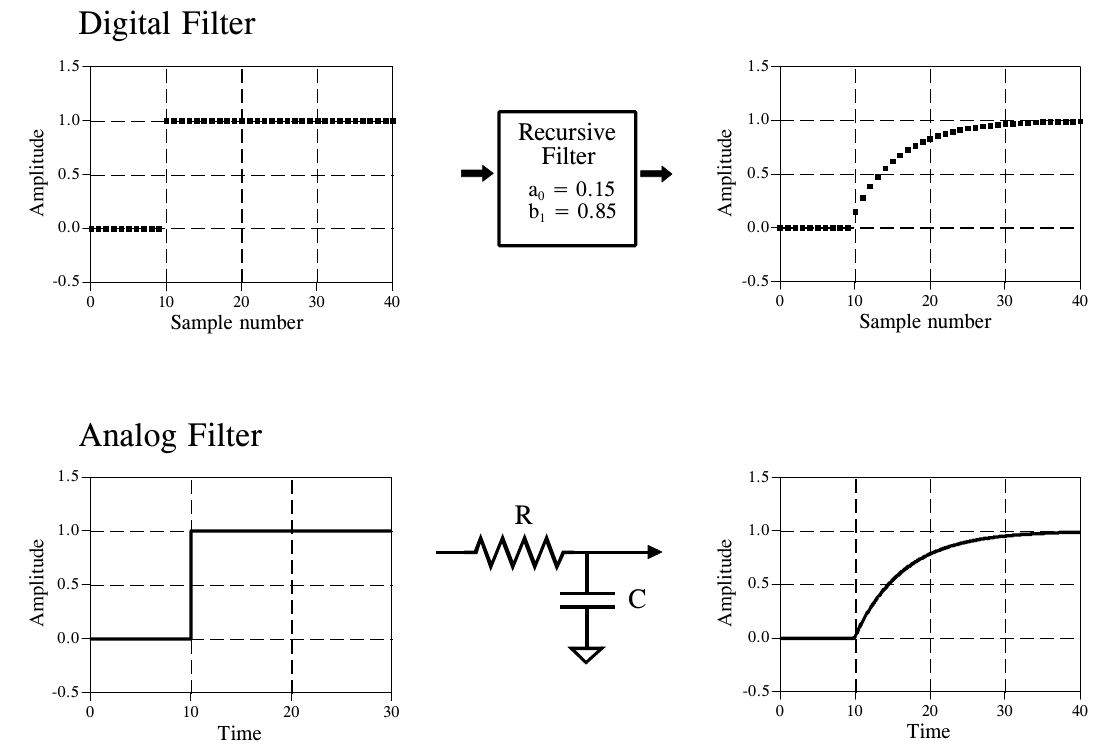
\includegraphics[width=0.921\linewidth,height=0.8\textheight,keepaspectratio]{assets/ch19/fig19-02.png}
\caption*{\textbf{图 19-2　单极点低通滤波器。}
数字递归滤波器可以模仿由电阻和电容组成的模拟滤波器。如本例所示，单极点低通递归滤波器会把阶跃输入的边沿变平滑，就像电子
RC 滤波器一样。 （Digital Filter = 数字滤波器，Recursive Filter =
递归滤波器，Analog Filter = 模拟滤波器；R = 电阻，C = 电容。Amplitude =
幅度，Sample number = 采样序号，Time = 时间。）}
\end{figure}

\section{单极点递归滤波器}

图 19-2 是一个所谓单极点低通滤波器(single pole low-pass
filter)的例子。这个递归滤波器只用两个系数：a₀ = 0.15 和 b₁ =
0.85。本例的输入信号是一个阶跃函数。正如你对低通滤波器的预期，输出平滑地上升到稳态值。这张图还展示了和你的电子学知识相关的一点：这个低通递归滤波器与由一个电阻和一个电容组成的电子低通滤波器完全相似。

递归方法的妙处在于，只改变少数几个参数，就能产生各种各样的响应。例如，图
19-3 是一个有三个系数的滤波器：a₀ = 0.93，a₁ = −0.93，b₁ =
0.86。从相似的阶跃响应可以看出，这个数字滤波器模仿的是电子 RC
高通滤波器。

\begin{figure}[htbp]
\centering
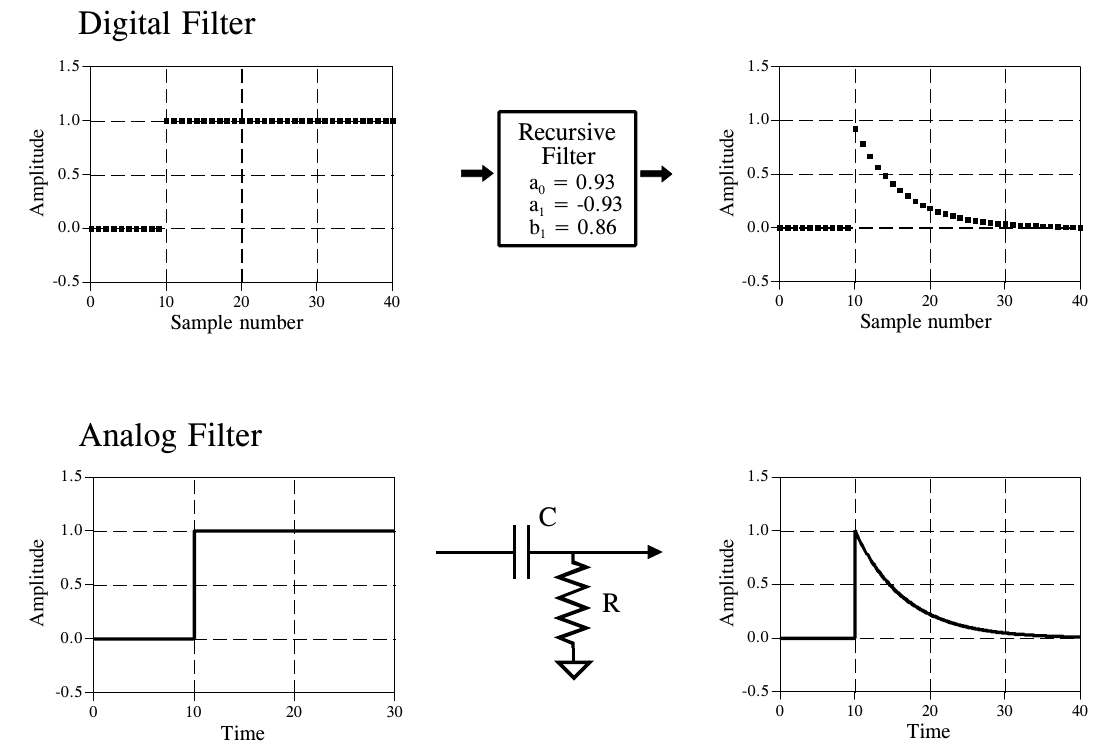
\includegraphics[width=0.921\linewidth,height=0.8\textheight,keepaspectratio]{assets/ch19/fig19-03.png}
\caption*{\textbf{图 19-3　单极点高通滤波器。}
选择合适的系数，也能让递归滤波器模仿电子 RC 高通滤波器。在 DSP
中可以像在模拟电子学里使用 RC 电路那样使用这些单极点递归滤波器。
（Digital Filter = 数字滤波器，Recursive Filter = 递归滤波器，Analog
Filter = 模拟滤波器；C = 电容，R = 电阻。Amplitude = 幅度，Sample number
= 采样序号，Time = 时间。）}
\end{figure}

这些单极点递归滤波器绝对值得放进你的 DSP 工具箱。你可以像用 RC
网络处理模拟电子信号那样，用它们处理数字信号。这包括你能想到的一切：去除直流、抑制高频噪声、波形整形、平滑等等。它们容易编程，执行快，很少出乎意料。系数由下面这些简单公式求出：

\textbf{公式 19-2}　单极点低通滤波器。滤波器的响应由参数 x 控制，x 取 0
到 1 之间的值。

\[a_0 = 1 - x \qquad b_1 = x\]

\textbf{公式 19-3}　单极点高通滤波器。

\[a_0 = \frac{1+x}{2} \qquad a_1 = -\frac{1+x}{2} \qquad b_1 = x\]

这些滤波器的特性由参数 x 控制，x 取 0 到 1 之间的值。物理上，x
是相邻采样之间的衰减量。例如，图 19-3 中 x 是
0.86，意思是输出信号中每个采样的值是它前一个采样的 0.86 倍。x
越大，衰减越慢。注意，如果 x
大于一，滤波器就会变得不稳定。也就是说，输入上任何一个非零值都会让输出不断增大，直到溢出。

x 的值可以直接指定，也可以从想要的滤波器时间常数(time
constant)求出。正如 R×C 是 RC 电路衰减到其最终值的 36.8\% 所需的秒数，d
是递归滤波器衰减到同样水平所需的采样数：

\textbf{公式 19-4}　单极点滤波器的时间常数。这个公式把相邻采样间的衰减量
x，与滤波器的时间常数 d（滤波器衰减到 36.8\% 所需的采样数）联系起来。

\[x = e^{-1/d}\]

例如，采样间衰减 x = 0.86 对应时间常数 d = 6.63 个采样（如图 19-3
所示）。x 与数字滤波器的 −3dB 截止频率 f\_C 之间也有一个固定关系：

\textbf{公式 19-5}　单极点滤波器的截止频率。采样间衰减量 x
与滤波器的截止频率 f\_C 相关，f\_C 取 0 到 0.5 之间的值。

\[x = e^{-2\pi f_C}\]

这样，求''a''和''b''系数就有了三种途径：从时间常数出发、从截止频率出发，或者直接挑一个
x。

图 19-4 是使用单极点递归滤波器的一个例子。(a)
中的原信号是一条平滑曲线，只是中间夹了一段高频正弦波的猝发(burst)。(b)
是信号经过低通和高通滤波器后的结果。两个信号分得相当好，但不完美，就像对模拟信号使用简单的
RC 电路一样。

\begin{figure}[htbp]
\centering
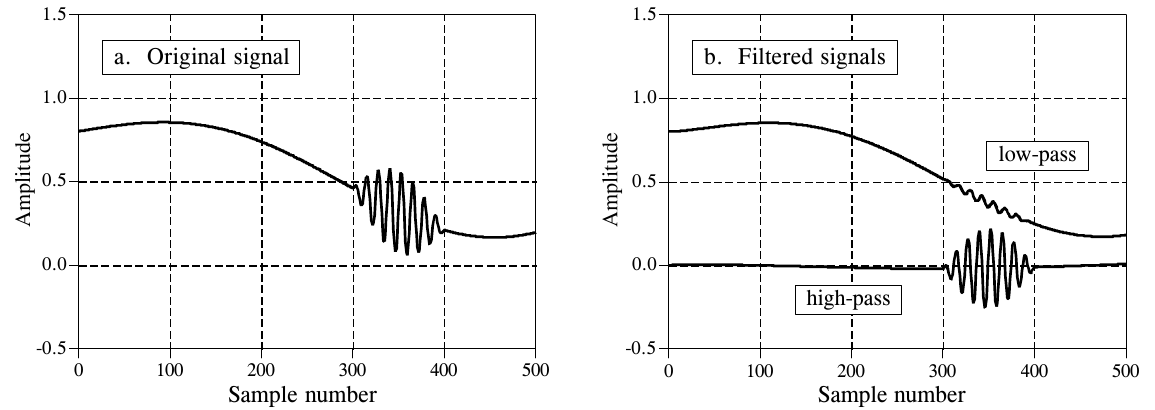
\includegraphics[width=0.963\linewidth,height=0.8\textheight,keepaspectratio]{assets/ch19/fig19-04.png}
\caption*{\textbf{图 19-4　单极点递归滤波器的例子。} (a)
中，一段高频猝发叠加在一个缓慢变化的信号上。(b)
中，用单极点低通和高通滤波器把这两个成分分开。低通滤波器用 x =
0.95，高通滤波器用 x = 0.86。 （a. Original signal = 原信号；b. Filtered
signals = 滤波后的信号；low-pass = 低通，high-pass = 高通。Amplitude =
幅度，Sample number = 采样序号。）}
\end{figure}

图 19-5
给出了几种单极点递归滤波器的频率响应。这些曲线的求法是：把一个冲激函数送进滤波器，得到滤波器的冲激响应，再用
FFT 把冲激响应变换成频率响应。原则上冲激响应无限长；但大约 15 到 20
个时间常数之后，它就衰减到单精度舍入噪声以下了。例如，滤波器的时间常数为
d = 6.63 个采样时，冲激响应大约 128 个采样就能装下。

\begin{figure}[htbp]
\centering
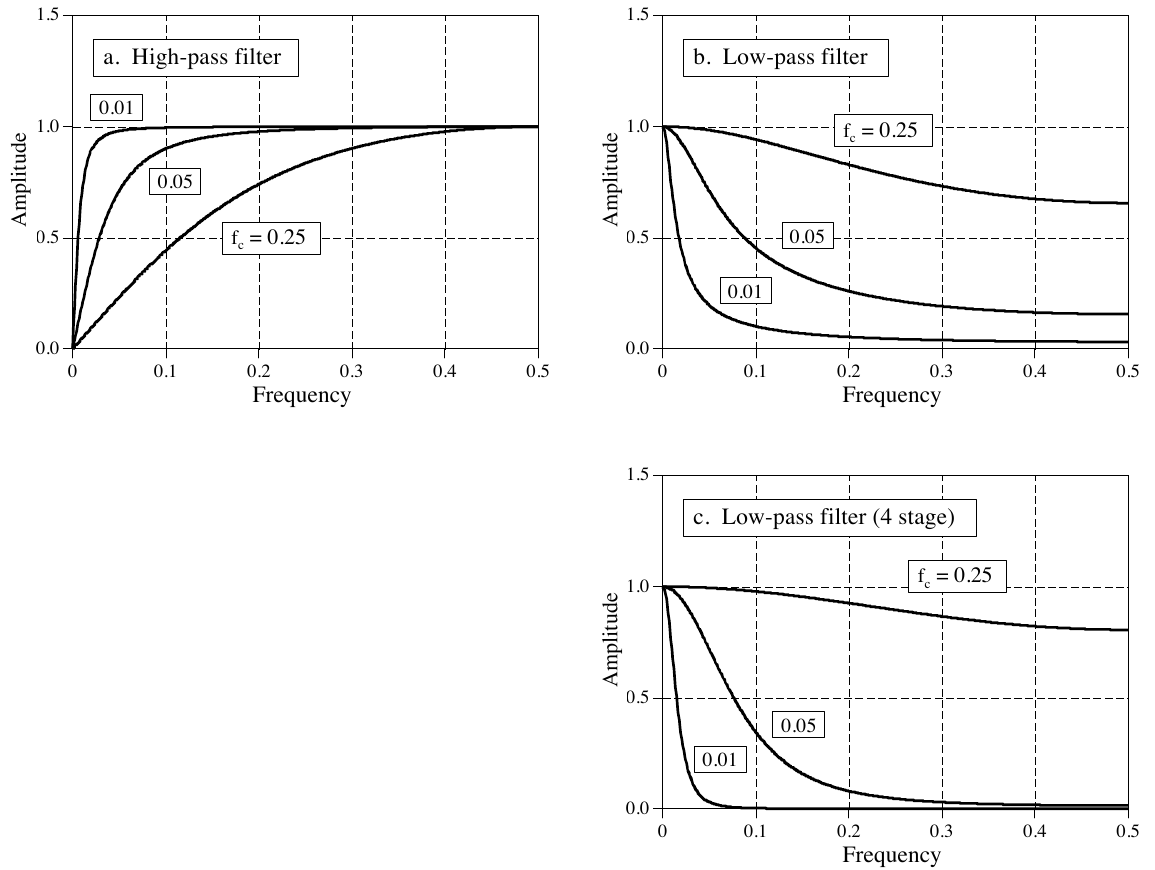
\includegraphics[width=0.963\linewidth,height=0.8\textheight,keepaspectratio]{assets/ch19/fig19-05.png}
\caption*{\textbf{图 19-5　单极点滤波器的频率响应。} (a) 和 (b)
分别是单极点高通和低通递归滤波器的频率响应。(c)
是四个低通滤波器级联的频率响应。递归滤波器的频率响应并不总是如你所料，尤其是把滤波器推到极限时。例如，(c)
中 f\_C = 0.25
的曲线几乎没用。原因有很多，包括：混叠、舍入噪声和非线性相位响应。 （a.
High-pass filter = 高通滤波器；b. Low-pass filter =
低通滤波器；c.~Low-pass filter (4 stage) = 低通滤波器（四级）。曲线旁的
0.01、0.05、f\_c = 0.25 是截止频率。Amplitude = 幅度，Frequency =
频率。）}
\end{figure}

图 19-5
的关键特点是：单极点递归滤波器分离不同频带的能力很差。换句话说，它们在时域表现很好，在频域表现很差。把几级级联起来，频率响应可以稍有改善。这有两种做法。第一，让信号多次通过同一个滤波器。第二，用
z 变换求出把级联合成单级的递归系数。两种方法都行得通，也都常用。(c)
是四个低通滤波器级联的频率响应。虽然阻带衰减显著改善，但滚降(roll-off)仍然很糟。如果你需要在频域有更好的性能，去看下一章的切比雪夫滤波器。

四级低通滤波器可以和布莱克曼(Blackman)滤波器、高斯(Gaussian)滤波器（移动平均滤波器的亲戚，见第
15 章）相媲美，但执行速度快得多。四级低通滤波器的设计公式是：

\textbf{公式
19-6}　四级低通滤波器。这些公式给出四个单极点低通滤波器级联后的''a''和''b''系数。x
与这个滤波器截止频率之间的关系由公式 19-5 给出，只是要把其中的 2π 换成
14.445。

\[a_0 = (1-x)^4 \qquad b_1 = 4x \qquad b_2 = -6x^2 \qquad b_3 = 4x^3 \qquad b_4 = -x^4\]

\section{窄带滤波器}

电子学和 DSP
中一个常见的需求，是从一个带宽较宽的信号中分离出一个窄频带。例如，你可能想消除仪器系统中的
60
赫兹干扰，或者分离出电话网络中的信令音。可用的频率响应有两类：带通(band-pass)和带阻（band-reject，也叫陷波滤波器(notch
filter)）。图 19-6
给出了这些滤波器的频率响应，递归系数由下面的公式给出：

\textbf{公式 19-7}　带通滤波器。频率响应的例子见图
19-6a。使用这些公式时，先选定中心频率 f 和带宽
BW，两者都用采样率的分数表示，因此在 0 到 0.5 之间。然后算出 R，再算出
K，最后算出递归系数。

\[a_0 = 1 - K \qquad a_1 = 2(K-R)\cos(2\pi f) \qquad a_2 = R^2 - K \qquad b_1 = 2R\cos(2\pi f) \qquad b_2 = -R^2\]

\textbf{公式
19-8}　带阻滤波器。这种滤波器通常叫陷波滤波器。频率响应的例子见图
19-6b。

\[a_0 = K \qquad a_1 = -2K\cos(2\pi f) \qquad a_2 = K \qquad b_1 = 2R\cos(2\pi f) \qquad b_2 = -R^2\]

其中：

\[K = \frac{1 - 2R\cos(2\pi f) + R^2}{2 - 2\cos(2\pi f)} \qquad R = 1 - 3\,BW\]

\begin{figure}[htbp]
\centering
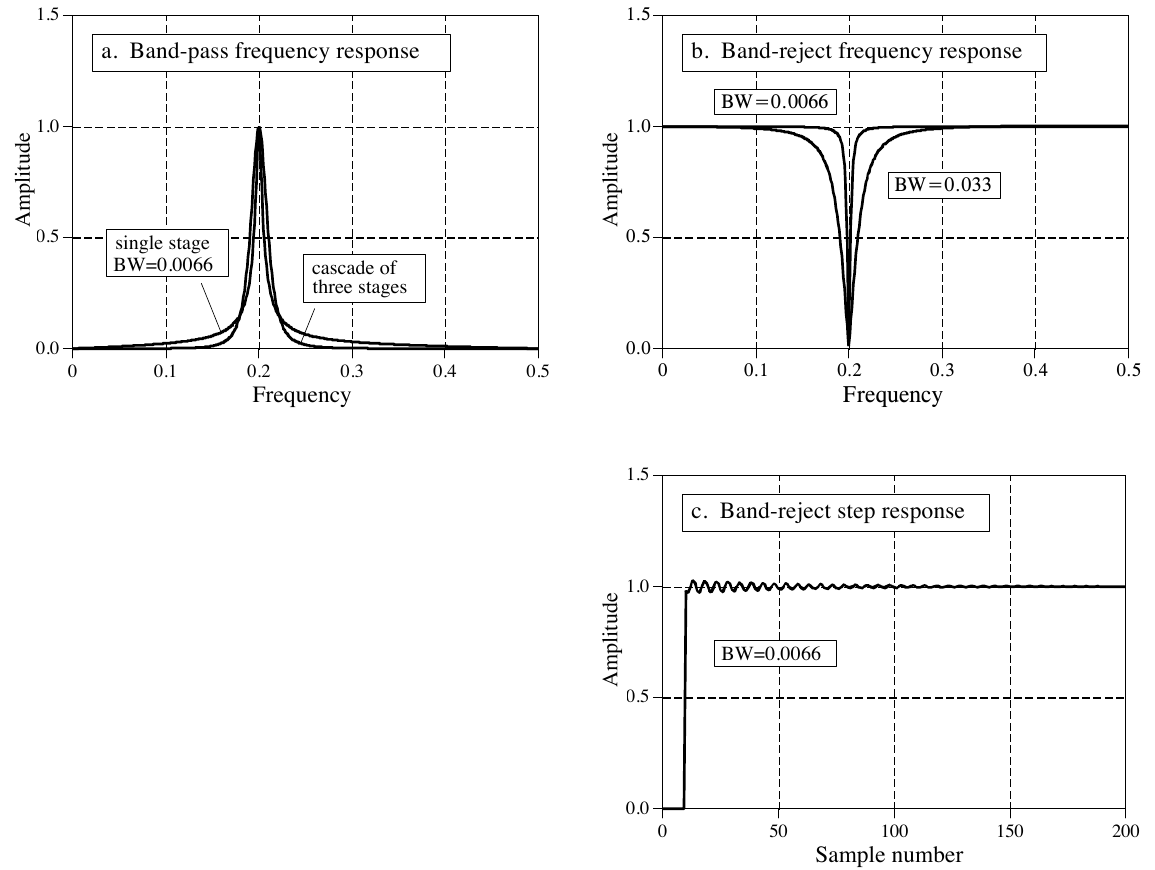
\includegraphics[width=0.963\linewidth,height=0.8\textheight,keepaspectratio]{assets/ch19/fig19-06.png}
\caption*{\textbf{图 19-6　窄带滤波器的特性。} (a) 和 (b)
是几种带通和带阻滤波器的频率响应。(c)
是带阻滤波器的阶跃响应。带阻（陷波）滤波器适合从时域编码的波形中去除 60
Hz 之类的干扰。 （a. Band-pass frequency response = 带通频率响应，single
stage = 单级，cascade of three stages = 三级级联；b. Band-reject
frequency response = 带阻频率响应；c.~Band-reject step response =
带阻阶跃响应。BW = 带宽。Amplitude = 幅度，Frequency = 频率，Sample
number = 采样序号。原书图注 ``Figure (a) and (b) shows''
主谓不一致，应为 show。）}
\end{figure}

使用这些公式之前，必须选定两个参数：中心频率 f，以及带宽 BW（在幅度
0.707 处测量）。两者都用采样频率的分数表示，因此必须在 0 到 0.5
之间。由这两个指定值先算出中间变量 R 和 K，再算出递归系数。

如 (a)
所示，带通滤波器的主峰两侧拖着相当大的尾巴。级联几级可以改善这一点。由于设计公式很长，实现这种级联更简单的办法是让信号多次通过滤波器，而不是去求单个滤波器所需的系数。

\begin{enumerate}
\def\labelenumi{(\alph{enumi})}
\setcounter{enumi}{1}
\tightlist
\item
  是带阻滤波器的例子。用单精度能得到的最窄带宽约为采样频率的
  0.0003。超过这个极限，陷波的衰减就会变差。(c)
  是带阻滤波器的阶跃响应。有明显的过冲(overshoot)和振铃(ringing)，但幅度很小。这使得这种滤波器能去除窄带干扰（60
  Hz 之类），而对时域波形只造成很小的失真。
\end{enumerate}

\section{相位响应}

滤波器的相位响应有三种类型：零相位、线性相位和非线性相位。图 19-7
给出了每种类型的一个例子。如 (a)
所示，零相位滤波器的特征是冲激响应关于第 0
个采样对称。具体形状无关紧要，只要负序号的采样是正序号采样的镜像就行。对这种对称波形做傅里叶变换，相位将全部为零，如
(b) 所示。

零相位滤波器的缺点是需要用负下标，处理起来可能不方便。线性相位滤波器是绕开这个问题的办法。(d)
中的冲激响应与 (a)
完全相同，只是平移到只用正序号的采样。冲激响应仍然左右对称，但对称位置从零移开了。这个平移使得相位
(e)
成为一条直线，``线性相位''由此得名。这条直线的斜率与平移量成正比。由于冲激响应的平移只会让输出信号产生同样的平移，在大多数用途中，线性相位滤波器与零相位滤波器是等价的。

\begin{enumerate}
\def\labelenumi{(\alph{enumi})}
\setcounter{enumi}{6}
\tightlist
\item
  是一个左右不对称的冲激响应。相应地，相位 (h)
  不是一条直线，也就是非线性相位。别把''非线性相位''和''线性相位''这两个术语，与第
  5 章讨论的系统线性的概念混淆。虽然都用了''线性''这个词，它们毫无关系。
\end{enumerate}

为什么有人在乎相位是不是线性的？(c)、(f) 和 (i)
给出了答案。这些是三个滤波器各自的脉冲响应(pulse
response)。脉冲响应无非是一个向上的阶跃响应，后面跟着一个向下的阶跃响应。这里用脉冲响应，是因为它能同时显示信号的上升沿和下降沿发生了什么。重点来了：零相位和线性相位滤波器的左右边沿看起来一样，而非线性相位滤波器的左右边沿看起来不一样。许多应用无法容忍左右边沿不一样。一个例子是示波器的显示，这种差异可能被误认为是被测信号本身的特征。另一个例子是视频处理。你能想象打开电视，发现你最喜欢的演员左耳和右耳长得不一样吗？

\begin{figure}[htbp]
\centering
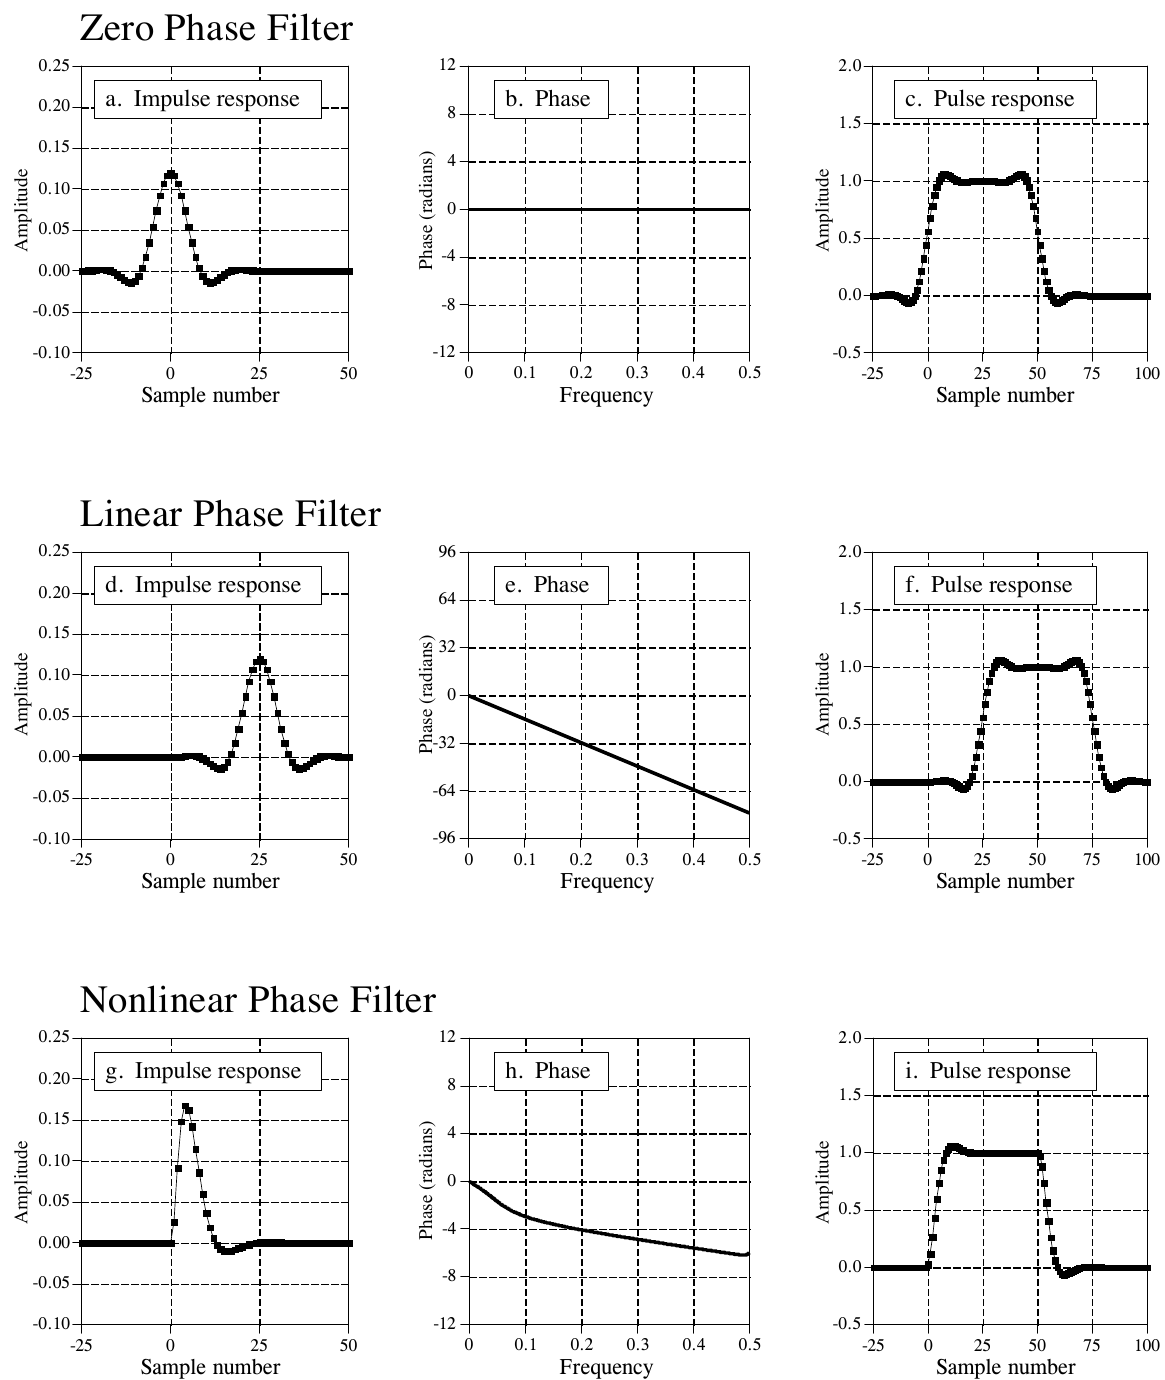
\includegraphics[width=0.971\linewidth,height=0.8\textheight,keepaspectratio]{assets/ch19/fig19-07.png}
\caption*{\textbf{图 19-7　零相位、线性相位和非线性相位滤波器。}
零相位滤波器的冲激响应关于第 0 个采样左右对称，如
(a)。这使得频率响应的相位全部为零，如
(b)。零相位冲激响应很理想，因为它们的阶跃响应上下对称，使脉冲的左右边沿看起来一样，如
(c) 所示。线性相位滤波器左右对称，但对称轴不在第 0 个采样，如 (d)
所示。这使得相位是线性的，即一条直线，如 (e) 所示。(f)
所示的线性相位脉冲响应具有零相位脉冲响应的所有优点。相比之下，非线性相位滤波器的冲激响应左右不对称，如
(g)，相位也不是直线，如 (h)。最糟的是，脉冲响应的左右边沿不一样，如 (i)
所示。 （Zero Phase Filter = 零相位滤波器，Linear Phase Filter =
线性相位滤波器，Nonlinear Phase Filter = 非线性相位滤波器；Impulse
response = 冲激响应，Phase = 相位，Pulse response = 脉冲响应。Amplitude
= 幅度，Phase (radians) = 相位（弧度），Frequency = 频率，Sample number
= 采样序号。(d) 横轴最左边的刻度在原书中显示为 25，应为 −25。）}
\end{figure}

让
FIR（有限冲激响应）滤波器具有线性相位很容易。这是因为在设计过程中冲激响应（滤波器核）是直接指定的，只要让滤波器核左右对称就行了。IIR（递归）滤波器则不然，因为指定的是递归系数，而不是冲激响应。递归滤波器的冲激响应左右不对称，因此是非线性相位的。

模拟电子电路在相位响应上也有同样的问题。设想你桌上放着一个由电阻和电容组成的电路。如果输入一直是零，输出也一直是零。给输入加一个冲激时，电容迅速充电到某个值，然后开始通过电阻按指数放电。冲激响应（即输出信号）是这些衰减指数的组合。冲激响应不可能对称，因为冲激之前输出为零，而指数衰减永远不会完全回到零。模拟滤波器设计者用贝塞尔滤波器(Bessel
filter)来对付这个问题，见第 3
章。贝塞尔滤波器被设计成相位尽可能线性，但远远比不上数字滤波器的性能。能够提供精确的线性相位，是数字滤波器的一个明显优势。

幸运的是，有一种简单的方法可以把递归滤波器改造成零相位。图 19-8
是这种方法的一个例子。(a) 是要滤波的输入信号。(b)
是经过单极点低通滤波器后的信号。由于这是非线性相位滤波器，左右边沿看起来不一样，它们互为倒置的版本。如前所述，这个递归滤波器的实现方式是从第
0 个采样开始，向第 150 个采样推进，沿途逐个计算每个采样。

现在假设我们不从第 0 个采样向第 150 个推进，而是从第 150 个采样开始向第
0
个推进。换句话说，输出信号的每个采样，由正在计算的采样右边的输入和输出采样算出。这意味着递归方程（公式
19-1）变为：

\textbf{公式 19-9}　反向递归方程。它与公式 19-1
相同，只是信号从右往左滤波，而不是从左往右。

\[\begin{aligned} y[n] = {}& a_0\,x[n] + a_1\,x[n+1] + a_2\,x[n+2] + a_3\,x[n+3] + \cdots \\ & + b_1\,y[n+1] + b_2\,y[n+2] + b_3\,y[n+3] + \cdots \end{aligned}\]

\begin{quote}
\textbf{译注：} 原书公式 19-9 的说明写成 ``filtered from left-to-right,
instead of
right-to-left''（从左往右、而不是从右往左），方向正好说反了。公式里用的是
n+1、n+2 等右边的点，应为从右往左滤波，译文已按正确方向翻译。
\end{quote}

\begin{enumerate}
\def\labelenumi{(\alph{enumi})}
\setcounter{enumi}{2}
\tightlist
\item
  是这种反向滤波的结果。这相当于让模拟信号通过一个电子 RC
  电路，同时让时间倒流。原书这里有一句倒着写的玩笑话，正过来读是：``Caution-
  time reversal can screw-up the
  universe!''（注意：时间倒流可能会把宇宙搞乱！）
\end{enumerate}

反向滤波本身没有任何好处：滤波后的信号左右边沿仍然不一样。奇迹发生在正向和反向滤波结合起来的时候。(d)
是先正向滤波、再反向滤波一次的结果。瞧！这就得到了一个零相位递归滤波器。实际上，任何递归滤波器都能用这种双向滤波(bidirectional
filtering)技术变成零相位。为这种性能提升付出的唯一代价，是执行时间和程序复杂度都变成两倍。

\begin{figure}[htbp]
\centering
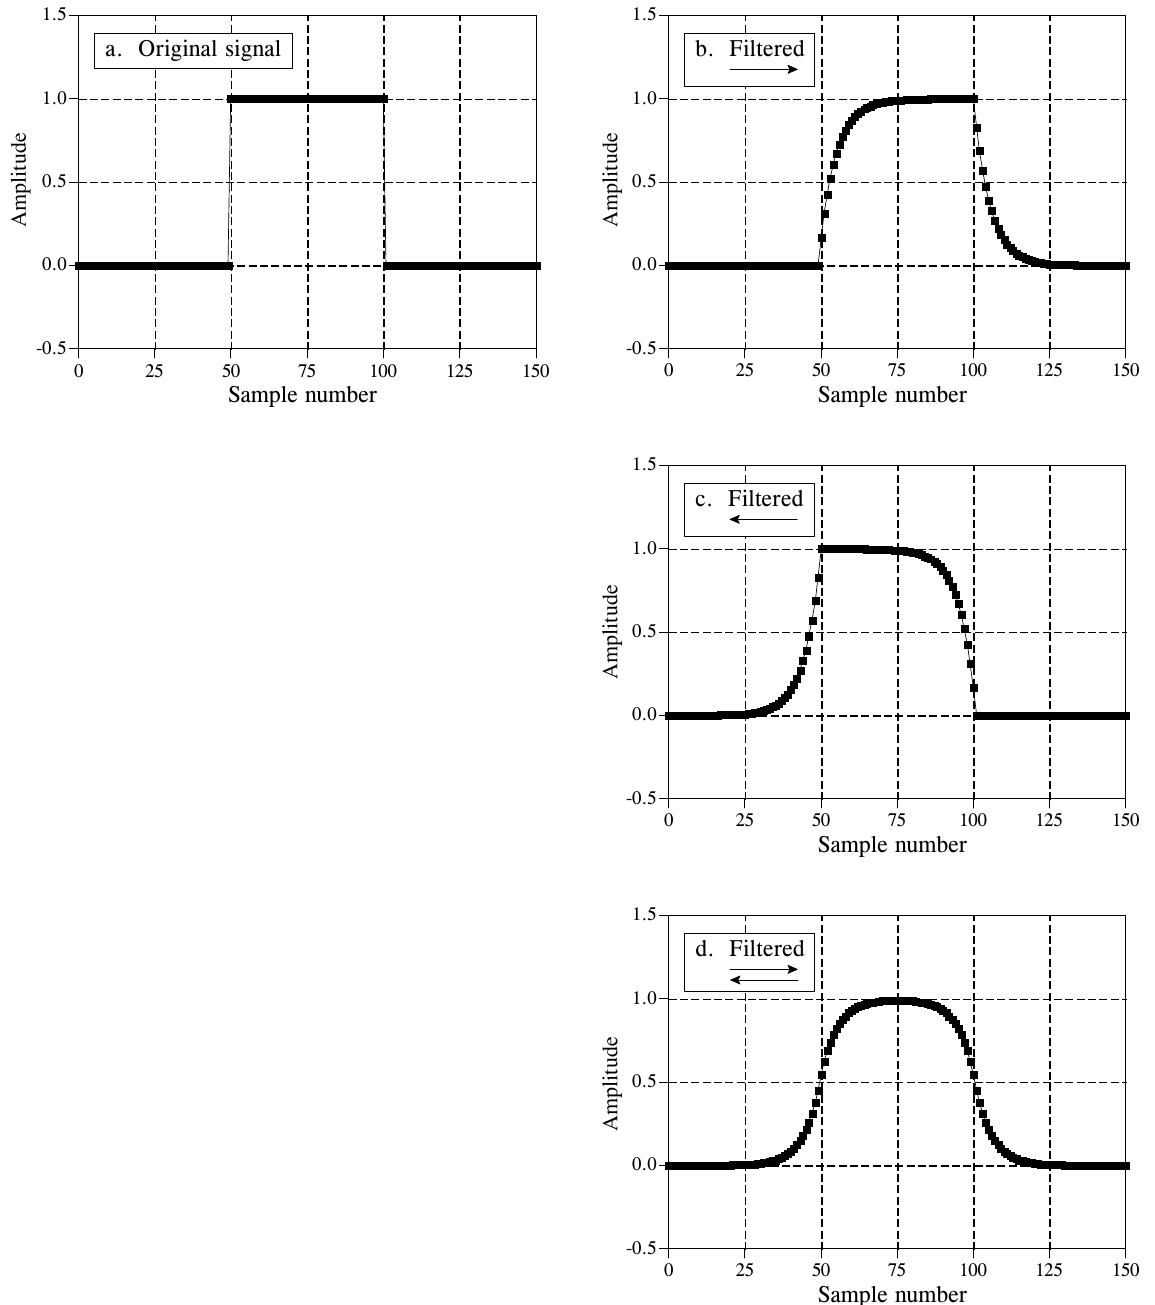
\includegraphics[width=0.963\linewidth,height=0.8\textheight,keepaspectratio]{assets/ch19/fig19-08.png}
\caption*{\textbf{图 19-8　双向递归滤波。} (a) 是矩形脉冲输入信号。(b)
是用单极点递归低通滤波器从左往右滤波后的信号。(c)
中信号以同样方式处理，只是滤波器从右往左移动。(d)
是先从左往右、再从右往左滤波后的信号。任何递归滤波器都能用这种技术变成零相位。
（a. Original signal = 原信号；b、c、d.~Filtered =
滤波后，框中箭头表示滤波方向：\dspsym{→} 从左往右，\dspsym{←}
从右往左，\dspsym{⇄} 双向。Amplitude = 幅度，Sample number =
采样序号。）}
\end{figure}

整个滤波器的冲激响应和频率响应怎么求？频率响应的幅度在两个方向上相同，而相位符号相反。两个方向合起来时，幅度变成平方，相位相互抵消为零。在时域中，这相当于把原冲激响应与它自身左右翻转的版本做卷积。例如，单极点低通滤波器的冲激响应是一个单边指数。相应的双向滤波器的冲激响应，是一个向右衰减的单边指数，与一个向左衰减的单边指数的卷积。推一下数学，结果是一个向左右两边都衰减的双边指数，衰减常数与原滤波器相同。

有些应用在某一时刻只有信号的一部分在计算机里，比如持续交替输入和输出数据的系统。这种情况下，可以把双向滤波与上一章讲的重叠相加法(overlap-add
method)结合使用。当你遇到冲激响应有多长这个问题时，别说''无限长''。要是这么说，你就得给每个信号段补上无限多个零。记住，冲激响应衰减到舍入噪声水平以下（大约
15 到 20
个时间常数）后就可以截断。每一段都需要在左右两边补零，以容纳双向滤波过程中的扩展。

\section{使用整数}

单精度浮点数非常适合实现这些简单的递归滤波器。用整数也可以，但要难得多。主要有两个问题。第一，有限位数带来的舍入误差会降低滤波器的响应，甚至使它不稳定。第二，递归系数的小数值必须用整数运算来处理。解决这个问题的一种办法，是把每个系数表示成一个分数。例如，0.15
变成 19/128。不再乘以 0.15，而是先乘以 19，再除以
128。另一种办法是用查找表(look-up table)代替乘法。例如，一个 12 位 ADC
产生的采样值在 0 到 4095 之间。不必把每个采样乘以
0.15，而是让采样通过一个 4096
项长的查找表，从表里取出的值就等于进入查找表的值乘以
0.15。这种方法非常快，但需要额外的内存：每个系数都需要一张单独的查找表。在尝试这两种整数方法之前，先确认移动平均滤波器的递归算法满足不了你的需求。它最爱整数。

% !TEX root = ../main.tex
% 本文件由 build-tex.sh 从 20-DSP指南-第20章中译.md 生成，改内容请改 md 后重新生成

\chapter{切比雪夫滤波器}\label{ch-20}

切比雪夫滤波器(Chebyshev
filter)用来把一个频带与另一个频带分开。它们的性能虽然比不上加窗 sinc
滤波器，但对许多应用来说已经绰绰有余。切比雪夫滤波器最主要的优点是速度快，通常比加窗
sinc
滤波器快一个数量级以上。这是因为它们靠递归(recursion)而不是卷积来实现。这类滤波器的设计基于一种叫
z 变换(z-transform)的数学技术，第 33
章会讲到。本章给出使用切比雪夫滤波器所需的信息，让你不必在高等数学的泥潭里跋涉。

\section{切比雪夫响应与巴特沃斯响应}

切比雪夫响应(Chebyshev
response)是一种数学策略：允许频率响应中出现纹波(ripple)，以换取更快的滚降(roll-off)。采用这种方法的模拟和数字滤波器都叫切比雪夫滤波器。例如，第
3
章中的模数转换和数模转换就用到了模拟切比雪夫滤波器。这些滤波器的名字来自它们使用的切比雪夫多项式(Chebyshev
polynomials)，由俄国数学家帕夫努季·切比雪夫(Pafnuti
Chebyshev，1821--1894)提出。这个名字是从俄语音译过来的，在文献中有多种拼法，比如
Chebychev、Tschebyscheff、Tchebysheff 和 Tchebichef。

图 20-1 给出了通带纹波分别为 0\%、0.5\% 和 20\%
的低通切比雪夫滤波器的频率响应。纹波越大（坏事），滚降就越陡（好事）。切比雪夫响应是这两个参数之间的最优折中。纹波设为
0\% 时，这种滤波器叫最大平坦(maximally
flat)滤波器或巴特沃斯滤波器(Butterworth filter)，以英国工程师 S.
Butterworth 的名字命名，他在 1930
年描述了这种响应。对数字滤波器来说，0.5\%
的纹波往往是个好选择，这与信号之前经过的模拟电路的典型精度和准确度相当。

\begin{figure}[htbp]
\centering
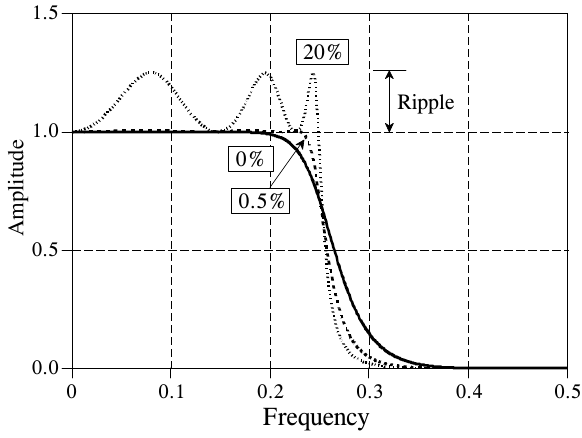
\includegraphics[width=0.485\linewidth,height=0.8\textheight,keepaspectratio]{assets/ch20/fig20-01.png}
\caption*{\textbf{图 20-1　切比雪夫响应。}
切比雪夫滤波器通过允许通带中出现纹波，来获得更快的滚降。纹波设为 0\%
时，叫最大平坦滤波器或巴特沃斯滤波器。设计时可以考虑用 0.5\%
的纹波：这么小的通带不平坦在这张图里根本看不出来，但滚降比巴特沃斯快得多。
（Amplitude = 幅度，Frequency = 频率，Ripple = 纹波；曲线旁的
0\%、0.5\%、20\% 是通带纹波。）}
\end{figure}

本章讨论的切比雪夫滤波器叫 I 型(type
1)滤波器，意思是只允许通带中有纹波。相比之下，II 型(type
2)切比雪夫滤波器只在阻带中有纹波。II
型滤波器很少用，我们不讨论。不过，有一种重要的设计叫椭圆滤波器(elliptic
filter)，它在通带和阻带中都有纹波。对给定的极点数，椭圆滤波器的滚降最快，但设计起来难得多。这里不讨论椭圆滤波器，但要知道，无论在模拟电子学还是
DSP
中，它常常是专业滤波器设计师的首选。如果你需要这种级别的性能，就去买一个设计数字滤波器的软件包吧。

\section{设计滤波器}

设计一个切比雪夫滤波器要选定四个参数：(1) 高通还是低通响应，(2)
截止频率，(3) 通带纹波的百分比，(4)
极点(pole)数。极点到底是什么？这里有两个答案，不喜欢其中一个，也许另一个能帮上忙：

\textbf{答案 1：} 拉普拉斯变换(Laplace transform)和 z
变换，是把冲激响应分解为正弦波和衰减指数的数学方法。具体做法是把系统的特性表示为一个复多项式除以另一个复多项式。分子的根叫零点(zero)，分母的根叫极点。由于极点和零点可以是复数，人们常说它们在复平面上有一个''位置''。复杂的系统比简单的系统有更多的极点和零点。设计递归滤波器时，先选定极点和零点的位置，再求出相应的递归系数（或模拟元件参数）。例如，巴特沃斯滤波器的极点位于复平面上的一个圆上，而切比雪夫滤波器的极点位于一个椭圆上。这是第
32 章和第 33 章的主题。

\textbf{答案 2：}
极点是装满魔粉的容器。滤波器里的极点越多，滤波器就越好用。

\begin{figure}[htbp]
\centering
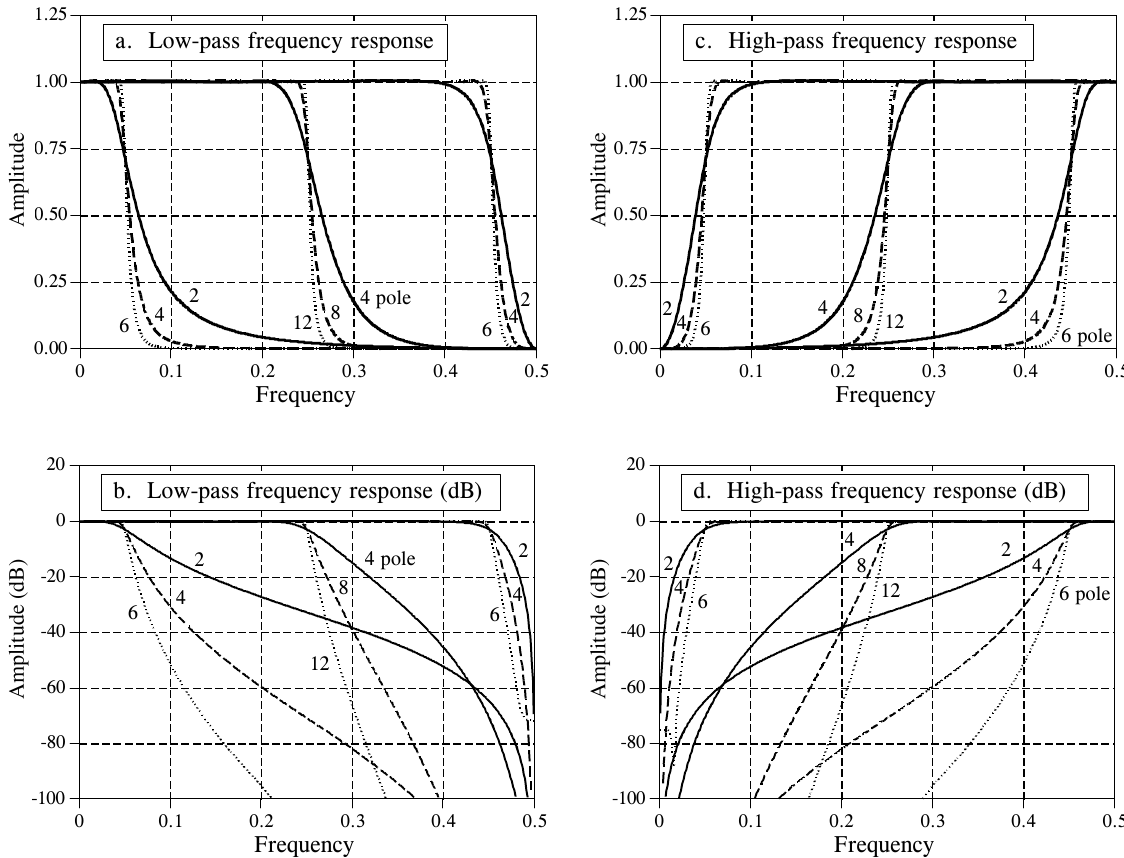
\includegraphics[width=0.937\linewidth,height=0.8\textheight,keepaspectratio]{assets/ch20/fig20-02.png}
\caption*{\textbf{图 20-2　切比雪夫频率响应。} (a) 和 (b) 是纹波 0.5\%
的低通切比雪夫滤波器的频率响应，(c) 和 (d) 是对应的高通滤波器响应。 （a.
Low-pass frequency response = 低通频率响应；b. Low-pass frequency
response (dB) = 低通频率响应（分贝）；c.~High-pass frequency response =
高通频率响应；d.~High-pass frequency response (dB) =
高通频率响应（分贝）。Amplitude = 幅度，Amplitude (dB) =
幅度（分贝），Frequency = 频率；曲线旁的数字是极点数，``4 pole'' = 4
极点。）}
\end{figure}

玩笑归玩笑，要点是：你完全可以不懂背后那套讨厌的数学，照样把这些滤波器用得很好。滤波器设计是一门专门的学问。实际工作中，按答案
2 思考的工程师、科学家和程序员，比按答案 1 思考的多。

图 20-2 给出了几个纹波为 0.5\%
的切比雪夫滤波器的频率响应。对这里用的方法来说，极点数必须是偶数。每个滤波器的截止频率，在幅度穿过
0.707（−3 dB）的地方测量。截止频率靠近 0 或 0.5
的滤波器，比位于频率范围中部的滤波器滚降更陡。例如，\(f_C = 0.05\)
的两极点滤波器，和 \(f_C = 0.25\)
的四极点滤波器滚降差不多。这很幸运：由于舍入噪声(round-off
noise)的缘故，在 0 和 0.5 附近只能用较少的极点。后面会细说。

不用 z 变换求递归系数的办法有两种。第一种是懦夫的办法：查表。表 20-1
和表 20-2 给出了通带纹波 0.5\%
的低通和高通滤波器的递归系数。如果你只需要一个快速粗糙的设计，把相应的系数抄进程序就完事了。

\textbf{表 20-1　低通切比雪夫滤波器（纹波 0.5\%）}

原书按截止频率 \(f_C\)
分行、按极点数分三栏排列，这里改成每种极点数一张表。为便于阅读，科学计数法写成
\texttt{1.234567e-4} 的形式（原书写作
\texttt{1.234567E-04}），数值逐位照抄原书。标 \dspsym{⚠} 的行原书注明
``!! Unstable !!''（不稳定），见后面''稳定性''一节。

\textbf{2 极点}

\begingroup\footnotesize\setlength{\tabcolsep}{3pt}

{\def\LTcaptype{none} % do not increment counter
\begin{longtable}[]{@{}
  >{\raggedright\arraybackslash}p{(\linewidth - 10\tabcolsep) * \real{0.1667}}
  >{\raggedright\arraybackslash}p{(\linewidth - 10\tabcolsep) * \real{0.1667}}
  >{\raggedright\arraybackslash}p{(\linewidth - 10\tabcolsep) * \real{0.1667}}
  >{\raggedright\arraybackslash}p{(\linewidth - 10\tabcolsep) * \real{0.1667}}
  >{\raggedright\arraybackslash}p{(\linewidth - 10\tabcolsep) * \real{0.1667}}
  >{\raggedright\arraybackslash}p{(\linewidth - 10\tabcolsep) * \real{0.1667}}@{}}
\toprule\noalign{}
\begin{minipage}[b]{\linewidth}\raggedright
fC
\end{minipage} & \begin{minipage}[b]{\linewidth}\raggedright
a0
\end{minipage} & \begin{minipage}[b]{\linewidth}\raggedright
a1
\end{minipage} & \begin{minipage}[b]{\linewidth}\raggedright
a2
\end{minipage} & \begin{minipage}[b]{\linewidth}\raggedright
b1
\end{minipage} & \begin{minipage}[b]{\linewidth}\raggedright
b2
\end{minipage} \\
\midrule\noalign{}
\endhead
\bottomrule\noalign{}
\endlastfoot
0.01 & 8.663387e-4 & 1.732678e-3 & 8.663387e-4 & 1.919129 &
-9.225943e-1 \\
0.025 & 5.112374e-3 & 1.022475e-2 & 5.112374e-3 & 1.797154 &
-8.176033e-1 \\
0.05 & 1.868823e-2 & 3.737647e-2 & 1.868823e-2 & 1.593937 &
-6.686903e-1 \\
0.075 & 3.869430e-2 & 7.738860e-2 & 3.869430e-2 & 1.392667 &
-5.474446e-1 \\
0.1 & 6.372802e-2 & 1.274560e-1 & 6.372802e-2 & 1.194365 &
-4.492774e-1 \\
0.15 & 1.254285e-1 & 2.508570e-1 & 1.254285e-1 & 8.070778e-1 &
-3.087918e-1 \\
0.2 & 1.997396e-1 & 3.994792e-1 & 1.997396e-1 & 4.291048e-1 &
-2.280633e-1 \\
0.25 & 2.858110e-1 & 5.716221e-1 & 2.858110e-1 & 5.423258e-2 &
-1.974768e-1 \\
0.3 & 3.849163e-1 & 7.698326e-1 & 3.849163e-1 & -3.249116e-1 &
-2.147536e-1 \\
0.35 & 5.001024e-1 & 1.000205 & 5.001024e-1 & -7.158993e-1 &
-2.845103e-1 \\
0.40 & 6.362308e-1 & 1.272462 & 6.362308e-1 & -1.125379 &
-4.195441e-1 \\
0.45 & 8.001101e-1 & 1.600220 & 8.001101e-1 & -1.556269 &
-6.441713e-1 \\
\end{longtable}
}

\endgroup

\textbf{4 极点}

\begingroup\scriptsize\setlength{\tabcolsep}{3pt}

{\def\LTcaptype{none} % do not increment counter
\begin{longtable}[]{@{}
  >{\raggedright\arraybackslash}p{(\linewidth - 18\tabcolsep) * \real{0.1000}}
  >{\raggedright\arraybackslash}p{(\linewidth - 18\tabcolsep) * \real{0.1000}}
  >{\raggedright\arraybackslash}p{(\linewidth - 18\tabcolsep) * \real{0.1000}}
  >{\raggedright\arraybackslash}p{(\linewidth - 18\tabcolsep) * \real{0.1000}}
  >{\raggedright\arraybackslash}p{(\linewidth - 18\tabcolsep) * \real{0.1000}}
  >{\raggedright\arraybackslash}p{(\linewidth - 18\tabcolsep) * \real{0.1000}}
  >{\raggedright\arraybackslash}p{(\linewidth - 18\tabcolsep) * \real{0.1000}}
  >{\raggedright\arraybackslash}p{(\linewidth - 18\tabcolsep) * \real{0.1000}}
  >{\raggedright\arraybackslash}p{(\linewidth - 18\tabcolsep) * \real{0.1000}}
  >{\raggedright\arraybackslash}p{(\linewidth - 18\tabcolsep) * \real{0.1000}}@{}}
\toprule\noalign{}
\begin{minipage}[b]{\linewidth}\raggedright
fC
\end{minipage} & \begin{minipage}[b]{\linewidth}\raggedright
a0
\end{minipage} & \begin{minipage}[b]{\linewidth}\raggedright
a1
\end{minipage} & \begin{minipage}[b]{\linewidth}\raggedright
a2
\end{minipage} & \begin{minipage}[b]{\linewidth}\raggedright
a3
\end{minipage} & \begin{minipage}[b]{\linewidth}\raggedright
a4
\end{minipage} & \begin{minipage}[b]{\linewidth}\raggedright
b1
\end{minipage} & \begin{minipage}[b]{\linewidth}\raggedright
b2
\end{minipage} & \begin{minipage}[b]{\linewidth}\raggedright
b3
\end{minipage} & \begin{minipage}[b]{\linewidth}\raggedright
b4
\end{minipage} \\
\midrule\noalign{}
\endhead
\bottomrule\noalign{}
\endlastfoot
0.01 \dspsym{⚠} & 4.149425e-7 & 1.659770e-6 & 2.489655e-6 & 1.659770e-6
& 4.149425e-7 & 3.893453 & -5.688233 & 3.695783 & -9.010106e-1 \\
0.025 & 1.504626e-5 & 6.018503e-5 & 9.027754e-5 & 6.018503e-5 &
1.504626e-5 & 3.725385 & -5.226004 & 3.270902 & -7.705239e-1 \\
0.05 & 2.141509e-4 & 8.566037e-4 & 1.284906e-3 & 8.566037e-4 &
2.141509e-4 & 3.425455 & -4.479272 & 2.643718 & -5.933269e-1 \\
0.075 & 9.726342e-4 & 3.890537e-3 & 5.835806e-3 & 3.890537e-3 &
9.726342e-4 & 3.103944 & -3.774453 & 2.111238 & -4.562908e-1 \\
0.1 & 2.780755e-3 & 1.112302e-2 & 1.668453e-2 & 1.112302e-2 &
2.780755e-3 & 2.764031 & -3.122854 & 1.664554 & -3.502232e-1 \\
0.15 & 1.180009e-2 & 4.720034e-2 & 7.080051e-2 & 4.720034e-2 &
1.180009e-2 & 2.039039 & -2.012961 & 9.897915e-1 & -2.046700e-1 \\
0.2 & 3.224554e-2 & 1.289821e-1 & 1.934732e-1 & 1.289821e-1 &
3.224554e-2 & 1.265912 & -1.203878 & 5.405908e-1 & -1.185538e-1 \\
0.25 & 7.015301e-2 & 2.806120e-1 & 4.209180e-1 & 2.806120e-1 &
7.015301e-2 & 4.541481e-1 & -7.417536e-1 & 2.361222e-1 & -7.096476e-2 \\
0.3 & 1.335566e-1 & 5.342263e-1 & 8.013394e-1 & 5.342263e-1 &
1.335566e-1 & -3.904486e-1 & -6.784138e-1 & -1.412021e-2 &
-5.392238e-2 \\
0.35 & 2.340973e-1 & 9.363892e-1 & 1.404584 & 9.363892e-1 & 2.340973e-1
& -1.263672 & -1.080487 & -3.276296e-1 & -7.376791e-2 \\
0.40 & 3.896966e-1 & 1.558787 & 2.338180 & 1.558787 & 3.896966e-1 &
-2.161179 & -2.033992 & -8.789098e-1 & -1.610655e-1 \\
0.45 & 6.291693e-1 & 2.516677 & 3.775016 & 2.516677 & 6.291693e-1 &
-3.077062 & -3.641323 & -1.949229 & -3.990945e-1 \\
\end{longtable}
}

\endgroup

\textbf{6 极点}

\begingroup\scriptsize\setlength{\tabcolsep}{3pt}

{\def\LTcaptype{none} % do not increment counter
\begin{longtable}[]{@{}
  >{\raggedright\arraybackslash}p{(\linewidth - 26\tabcolsep) * \real{0.0714}}
  >{\raggedright\arraybackslash}p{(\linewidth - 26\tabcolsep) * \real{0.0714}}
  >{\raggedright\arraybackslash}p{(\linewidth - 26\tabcolsep) * \real{0.0714}}
  >{\raggedright\arraybackslash}p{(\linewidth - 26\tabcolsep) * \real{0.0714}}
  >{\raggedright\arraybackslash}p{(\linewidth - 26\tabcolsep) * \real{0.0714}}
  >{\raggedright\arraybackslash}p{(\linewidth - 26\tabcolsep) * \real{0.0714}}
  >{\raggedright\arraybackslash}p{(\linewidth - 26\tabcolsep) * \real{0.0714}}
  >{\raggedright\arraybackslash}p{(\linewidth - 26\tabcolsep) * \real{0.0714}}
  >{\raggedright\arraybackslash}p{(\linewidth - 26\tabcolsep) * \real{0.0714}}
  >{\raggedright\arraybackslash}p{(\linewidth - 26\tabcolsep) * \real{0.0714}}
  >{\raggedright\arraybackslash}p{(\linewidth - 26\tabcolsep) * \real{0.0714}}
  >{\raggedright\arraybackslash}p{(\linewidth - 26\tabcolsep) * \real{0.0714}}
  >{\raggedright\arraybackslash}p{(\linewidth - 26\tabcolsep) * \real{0.0714}}
  >{\raggedright\arraybackslash}p{(\linewidth - 26\tabcolsep) * \real{0.0714}}@{}}
\toprule\noalign{}
\begin{minipage}[b]{\linewidth}\raggedright
fC
\end{minipage} & \begin{minipage}[b]{\linewidth}\raggedright
a0
\end{minipage} & \begin{minipage}[b]{\linewidth}\raggedright
a1
\end{minipage} & \begin{minipage}[b]{\linewidth}\raggedright
a2
\end{minipage} & \begin{minipage}[b]{\linewidth}\raggedright
a3
\end{minipage} & \begin{minipage}[b]{\linewidth}\raggedright
a4
\end{minipage} & \begin{minipage}[b]{\linewidth}\raggedright
a5
\end{minipage} & \begin{minipage}[b]{\linewidth}\raggedright
a6
\end{minipage} & \begin{minipage}[b]{\linewidth}\raggedright
b1
\end{minipage} & \begin{minipage}[b]{\linewidth}\raggedright
b2
\end{minipage} & \begin{minipage}[b]{\linewidth}\raggedright
b3
\end{minipage} & \begin{minipage}[b]{\linewidth}\raggedright
b4
\end{minipage} & \begin{minipage}[b]{\linewidth}\raggedright
b5
\end{minipage} & \begin{minipage}[b]{\linewidth}\raggedright
b6
\end{minipage} \\
\midrule\noalign{}
\endhead
\bottomrule\noalign{}
\endlastfoot
0.01 \dspsym{⚠} & 1.391351e-10 & 8.348109e-10 & 2.087027e-9 &
2.782703e-9 & 2.087027e-9 & 8.348109e-10 & 1.391351e-10 & 5.883343 &
-1.442798e1 & 1.887786e1 & -1.389914e1 & 5.459909 & -8.939932e-1 \\
0.025 \dspsym{⚠} & 3.136210e-8 & 1.881726e-7 & 4.704314e-7 & 6.272419e-7
& 4.704314e-7 & 1.881726e-7 & 3.136210e-8 & 5.691653 & -1.353172e1 &
1.719986e1 & -1.232689e1 & 4.722721 & -7.556340e-1 \\
0.05 & 1.771089e-6 & 1.062654e-5 & 2.656634e-5 & 3.542179e-5 &
2.656634e-5 & 1.062654e-5 & 1.771089e-6 & 5.330512 & -1.196611e1 &
1.447067e1 & -9.937710 & 3.673283 & -5.707561e-1 \\
0.075 & 1.797538e-5 & 1.078523e-4 & 2.696307e-4 & 3.595076e-4 &
2.696307e-4 & 1.078523e-4 & 1.797538e-5 & 4.921746 & -1.035734e1 &
1.189764e1 & -7.854533 & 2.822109 & -4.307710e-1 \\
0.1 & 9.086148e-5 & 5.451688e-4 & 1.362922e-3 & 1.817229e-3 &
1.362922e-3 & 5.451688e-4 & 9.086148e-5 & 4.470118 & -8.755594 &
9.543712 & -6.079376 & 2.140062 & -3.247363e-1 \\
0.15 & 8.618665e-4 & 5.171199e-3 & 1.292800e-2 & 1.723733e-2 &
1.292800e-2 & 5.171199e-3 & 8.618665e-4 & 3.455239 & -5.754735 &
5.645387 & -3.394902 & 1.177469 & -1.836195e-1 \\
0.2 & 4.187408e-3 & 2.512445e-2 & 6.281112e-2 & 8.374816e-2 &
6.281112e-2 & 2.512445e-2 & 4.187408e-3 & 2.315806 & -3.293726 &
2.904826 & -1.694128 & 6.021426e-1 & -1.029147e-1 \\
0.25 & 1.434449e-2 & 8.606697e-2 & 2.151674e-1 & 2.868899e-1 &
2.151674e-1 & 8.606697e-2 & 1.434449e-2 & 1.076052 & -1.662847 &
1.191063 & -7.403087e-1 & 2.752158e-1 & -5.722251e-2 \\
0.3 & 3.997487e-2 & 2.398492e-1 & 5.996231e-1 & 7.994975e-1 &
5.996231e-1 & 2.398492e-1 & 3.997487e-2 & -2.441152e-1 & -1.130306 &
1.063167e-1 & -3.463299e-1 & 8.882992e-2 & -3.278741e-2 \\
0.35 & 9.792321e-2 & 5.875393e-1 & 1.468848 & 1.958464 & 1.468848 &
5.875393e-1 & 9.792321e-2 & -1.627573 & -1.955020 & -1.075051 &
-5.106501e-1 & -7.239843e-2 & -2.639193e-2 \\
0.40 & 2.211834e-1 & 1.327100 & 3.317751 & 4.423668 & 3.317751 &
1.327100 & 2.211834e-1 & -3.058672 & -4.390465 & -3.523254 & -1.684185 &
-4.414881e-1 & -5.767513e-2 \\
0.45 & 4.760635e-1 & 2.856381 & 7.140952 & 9.521270 & 7.140952 &
2.856381 & 4.760635e-1 & -4.522403 & -8.676844 & -9.007512 & -5.328429 &
-1.702543 & -2.303303e-1 \\
\end{longtable}
}

\endgroup

\textbf{表 20-2　高通切比雪夫滤波器（纹波 0.5\%）}

排法同表 20-1。

\textbf{2 极点}

\begingroup\footnotesize\setlength{\tabcolsep}{3pt}

{\def\LTcaptype{none} % do not increment counter
\begin{longtable}[]{@{}
  >{\raggedright\arraybackslash}p{(\linewidth - 10\tabcolsep) * \real{0.1667}}
  >{\raggedright\arraybackslash}p{(\linewidth - 10\tabcolsep) * \real{0.1667}}
  >{\raggedright\arraybackslash}p{(\linewidth - 10\tabcolsep) * \real{0.1667}}
  >{\raggedright\arraybackslash}p{(\linewidth - 10\tabcolsep) * \real{0.1667}}
  >{\raggedright\arraybackslash}p{(\linewidth - 10\tabcolsep) * \real{0.1667}}
  >{\raggedright\arraybackslash}p{(\linewidth - 10\tabcolsep) * \real{0.1667}}@{}}
\toprule\noalign{}
\begin{minipage}[b]{\linewidth}\raggedright
fC
\end{minipage} & \begin{minipage}[b]{\linewidth}\raggedright
a0
\end{minipage} & \begin{minipage}[b]{\linewidth}\raggedright
a1
\end{minipage} & \begin{minipage}[b]{\linewidth}\raggedright
a2
\end{minipage} & \begin{minipage}[b]{\linewidth}\raggedright
b1
\end{minipage} & \begin{minipage}[b]{\linewidth}\raggedright
b2
\end{minipage} \\
\midrule\noalign{}
\endhead
\bottomrule\noalign{}
\endlastfoot
0.01 & 9.567529e-1 & -1.913506 & 9.567529e-1 & 1.911437 &
-9.155749e-1 \\
0.025 & 8.950355e-1 & -1.790071 & 8.950355e-1 & 1.777932 &
-8.022106e-1 \\
0.05 & 8.001102e-1 & -1.600220 & 8.001102e-1 & 1.556269 &
-6.441715e-1 \\
0.075 & 7.142028e-1 & -1.428406 & 7.142028e-1 & 1.338264 &
-5.185469e-1 \\
0.1 & 6.362307e-1 & -1.272461 & 6.362307e-1 & 1.125379 & -4.195440e-1 \\
0.15 & 5.001024e-1 & -1.000205 & 5.001024e-1 & 7.158993e-1 &
-2.845103e-1 \\
0.2 & 3.849163e-1 & -7.698326e-1 & 3.849163e-1 & 3.249116e-1 &
-2.147536e-1 \\
0.25 & 2.858111e-1 & -5.716222e-1 & 2.858111e-1 & -5.423243e-2 &
-1.974768e-1 \\
0.3 & 1.997396e-1 & -3.994792e-1 & 1.997396e-1 & -4.291049e-1 &
-2.280633e-1 \\
0.35 & 1.254285e-1 & -2.508570e-1 & 1.254285e-1 & -8.070777e-1 &
-3.087918e-1 \\
0.40 & 6.372801e-2 & -1.274560e-1 & 6.372801e-2 & -1.194365 &
-4.492774e-1 \\
0.45 & 1.868823e-2 & -3.737647e-2 & 1.868823e-2 & -1.593937 &
-6.686903e-1 \\
\end{longtable}
}

\endgroup

\textbf{4 极点}

\begingroup\scriptsize\setlength{\tabcolsep}{3pt}

{\def\LTcaptype{none} % do not increment counter
\begin{longtable}[]{@{}
  >{\raggedright\arraybackslash}p{(\linewidth - 18\tabcolsep) * \real{0.1000}}
  >{\raggedright\arraybackslash}p{(\linewidth - 18\tabcolsep) * \real{0.1000}}
  >{\raggedright\arraybackslash}p{(\linewidth - 18\tabcolsep) * \real{0.1000}}
  >{\raggedright\arraybackslash}p{(\linewidth - 18\tabcolsep) * \real{0.1000}}
  >{\raggedright\arraybackslash}p{(\linewidth - 18\tabcolsep) * \real{0.1000}}
  >{\raggedright\arraybackslash}p{(\linewidth - 18\tabcolsep) * \real{0.1000}}
  >{\raggedright\arraybackslash}p{(\linewidth - 18\tabcolsep) * \real{0.1000}}
  >{\raggedright\arraybackslash}p{(\linewidth - 18\tabcolsep) * \real{0.1000}}
  >{\raggedright\arraybackslash}p{(\linewidth - 18\tabcolsep) * \real{0.1000}}
  >{\raggedright\arraybackslash}p{(\linewidth - 18\tabcolsep) * \real{0.1000}}@{}}
\toprule\noalign{}
\begin{minipage}[b]{\linewidth}\raggedright
fC
\end{minipage} & \begin{minipage}[b]{\linewidth}\raggedright
a0
\end{minipage} & \begin{minipage}[b]{\linewidth}\raggedright
a1
\end{minipage} & \begin{minipage}[b]{\linewidth}\raggedright
a2
\end{minipage} & \begin{minipage}[b]{\linewidth}\raggedright
a3
\end{minipage} & \begin{minipage}[b]{\linewidth}\raggedright
a4
\end{minipage} & \begin{minipage}[b]{\linewidth}\raggedright
b1
\end{minipage} & \begin{minipage}[b]{\linewidth}\raggedright
b2
\end{minipage} & \begin{minipage}[b]{\linewidth}\raggedright
b3
\end{minipage} & \begin{minipage}[b]{\linewidth}\raggedright
b4
\end{minipage} \\
\midrule\noalign{}
\endhead
\bottomrule\noalign{}
\endlastfoot
0.01 \dspsym{⚠} & 9.121579e-1 & -3.648632 & 5.472947 & -3.648632 &
9.121579e-1 & 3.815952 & -5.465026 & 3.481295 & -8.322529e-1 \\
0.025 & 7.941874e-1 & -3.176750 & 4.765125 & -3.176750 & 7.941874e-1 &
3.538919 & -4.722213 & 2.814036 & -6.318300e-1 \\
0.05 & 6.291694e-1 & -2.516678 & 3.775016 & -2.516678 & 6.291694e-1 &
3.077062 & -3.641324 & 1.949230 & -3.990947e-1 \\
0.075 & 4.965350e-1 & -1.986140 & 2.979210 & -1.986140 & 4.965350e-1 &
2.617304 & -2.749252 & 1.325548 & -2.524546e-1 \\
0.1 & 3.896966e-1 & -1.558786 & 2.338179 & -1.558786 & 3.896966e-1 &
2.161179 & -2.033991 & 8.789094e-1 & -1.610655e-1 \\
0.15 & 2.340973e-1 & -9.363892e-1 & 1.404584 & -9.363892e-1 &
2.340973e-1 & 1.263672 & -1.080487 & 3.276296e-1 & -7.376791e-2 \\
0.2 & 1.335566e-1 & -5.342262e-1 & 8.013393e-1 & -5.342262e-1 &
1.335566e-1 & 3.904484e-1 & -6.784138e-1 & 1.412016e-2 & -5.392238e-2 \\
0.25 & 7.015302e-2 & -2.806121e-1 & 4.209182e-1 & -2.806121e-1 &
7.015302e-2 & -4.541478e-1 & -7.417535e-1 & -2.361221e-1 &
-7.096475e-2 \\
0.3 & 3.224553e-2 & -1.289821e-1 & 1.934732e-1 & -1.289821e-1 &
3.224553e-2 & -1.265912 & -1.203878 & -5.405908e-1 & -1.185538e-1 \\
0.35 & 1.180009e-2 & -4.720035e-2 & 7.080051e-2 & -4.720035e-2 &
1.180009e-2 & -2.039039 & -2.012961 & -9.897915e-1 & -2.046700e-1 \\
0.40 & 2.780754e-3 & -1.112302e-2 & 1.668453e-2 & -1.112302e-2 &
2.780754e-3 & -2.764031 & -3.122854 & -1.664554 & -3.502233e-1 \\
0.45 & 2.141509e-4 & -8.566037e-4 & 1.284906e-3 & -8.566037e-4 &
2.141509e-4 & -3.425455 & -4.479272 & -2.643718 & -5.933269e-1 \\
\end{longtable}
}

\endgroup

\textbf{6 极点}

\begingroup\scriptsize\setlength{\tabcolsep}{3pt}

{\def\LTcaptype{none} % do not increment counter
\begin{longtable}[]{@{}
  >{\raggedright\arraybackslash}p{(\linewidth - 26\tabcolsep) * \real{0.0714}}
  >{\raggedright\arraybackslash}p{(\linewidth - 26\tabcolsep) * \real{0.0714}}
  >{\raggedright\arraybackslash}p{(\linewidth - 26\tabcolsep) * \real{0.0714}}
  >{\raggedright\arraybackslash}p{(\linewidth - 26\tabcolsep) * \real{0.0714}}
  >{\raggedright\arraybackslash}p{(\linewidth - 26\tabcolsep) * \real{0.0714}}
  >{\raggedright\arraybackslash}p{(\linewidth - 26\tabcolsep) * \real{0.0714}}
  >{\raggedright\arraybackslash}p{(\linewidth - 26\tabcolsep) * \real{0.0714}}
  >{\raggedright\arraybackslash}p{(\linewidth - 26\tabcolsep) * \real{0.0714}}
  >{\raggedright\arraybackslash}p{(\linewidth - 26\tabcolsep) * \real{0.0714}}
  >{\raggedright\arraybackslash}p{(\linewidth - 26\tabcolsep) * \real{0.0714}}
  >{\raggedright\arraybackslash}p{(\linewidth - 26\tabcolsep) * \real{0.0714}}
  >{\raggedright\arraybackslash}p{(\linewidth - 26\tabcolsep) * \real{0.0714}}
  >{\raggedright\arraybackslash}p{(\linewidth - 26\tabcolsep) * \real{0.0714}}
  >{\raggedright\arraybackslash}p{(\linewidth - 26\tabcolsep) * \real{0.0714}}@{}}
\toprule\noalign{}
\begin{minipage}[b]{\linewidth}\raggedright
fC
\end{minipage} & \begin{minipage}[b]{\linewidth}\raggedright
a0
\end{minipage} & \begin{minipage}[b]{\linewidth}\raggedright
a1
\end{minipage} & \begin{minipage}[b]{\linewidth}\raggedright
a2
\end{minipage} & \begin{minipage}[b]{\linewidth}\raggedright
a3
\end{minipage} & \begin{minipage}[b]{\linewidth}\raggedright
a4
\end{minipage} & \begin{minipage}[b]{\linewidth}\raggedright
a5
\end{minipage} & \begin{minipage}[b]{\linewidth}\raggedright
a6
\end{minipage} & \begin{minipage}[b]{\linewidth}\raggedright
b1
\end{minipage} & \begin{minipage}[b]{\linewidth}\raggedright
b2
\end{minipage} & \begin{minipage}[b]{\linewidth}\raggedright
b3
\end{minipage} & \begin{minipage}[b]{\linewidth}\raggedright
b4
\end{minipage} & \begin{minipage}[b]{\linewidth}\raggedright
b5
\end{minipage} & \begin{minipage}[b]{\linewidth}\raggedright
b6
\end{minipage} \\
\midrule\noalign{}
\endhead
\bottomrule\noalign{}
\endlastfoot
0.01 \dspsym{⚠} & 8.630195e-1 & -5.178118 & 1.294529e1 & -1.726039e1 &
1.294529e1 & -5.178118 & 8.630195e-1 & 5.705102 & -1.356935e1 &
1.722231e1 & -1.230214e1 & 4.689218 & -7.451429e-1 \\
0.025 \dspsym{⚠} & 6.912863e-1 & -4.147718 & 1.036929e1 & -1.382573e1 &
1.036929e1 & -4.147718 & 6.912863e-1 & 5.261399 & -1.157800e1 &
1.363599e1 & -9.063840 & 3.223738 & -4.793541e-1 \\
0.05 & 4.760636e-1 & -2.856382 & 7.140954 & -9.521272 & 7.140954 &
-2.856382 & 4.760636e-1 & 4.522403 & -8.676846 & 9.007515 & -5.328431 &
1.702544 & -2.303304e-1 \\
0.075 & 3.259100e-1 & -1.955460 & 4.888651 & -6.518201 & 4.888651 &
-1.955460 & 3.259100e-1 & 3.787397 & -6.288362 & 5.747801 & -3.041570 &
8.808669e-1 & -1.122464e-1 \\
0.1 & 2.211833e-1 & -1.327100 & 3.317750 & -4.423667 & 3.317750 &
-1.327100 & 2.211833e-1 & 3.058671 & -4.390464 & 3.523252 & -1.684184 &
4.414878e-1 & -5.767508e-2 \\
0.15 & 9.792321e-2 & -5.875393e-1 & 1.468848 & -1.958464 & 1.468848 &
-5.875393e-1 & 9.792321e-2 & 1.627573 & -1.955020 & 1.075051 &
-5.106501e-1 & 7.239843e-2 & -2.639193e-2 \\
0.2 & 3.997486e-2 & -2.398492e-1 & 5.996230e-1 & -7.994973e-1 &
5.996230e-1 & -2.398492e-1 & 3.997486e-2 & 2.441149e-1 & -1.130306 &
-1.063169e-1 & -3.463299e-1 & -8.882996e-2 & -3.278741e-2 \\
0.25 & 1.434450e-2 & -8.606701e-2 & 2.151675e-1 & -2.868900e-1 &
2.151675e-1 & -8.606701e-2 & 1.434450e-2 & -1.076051 & -1.662847 &
-1.191062 & -7.403085e-1 & -2.752156e-1 & -5.722250e-2 \\
0.3 & 4.187407e-3 & -2.512444e-2 & 6.281111e-2 & -8.374815e-2 &
6.281111e-2 & -2.512444e-2 & 4.187407e-3 & -2.315806 & -3.293726 &
-2.904827 & -1.694129 & -6.021426e-1 & -1.029147e-1 \\
0.35 & 8.618665e-4 & -5.171200e-3 & 1.292800e-2 & -1.723733e-2 &
1.292800e-2 & -5.171200e-3 & 8.618665e-4 & -3.455239 & -5.754734 &
-5.645387 & -3.394902 & -1.177469 & -1.836195e-1 \\
0.40 & 9.086141e-5 & -5.451685e-4 & 1.362921e-3 & -1.817228e-3 &
1.362921e-3 & -5.451685e-4 & 9.086141e-5 & -4.470118 & -8.755595 &
-9.543712 & -6.079377 & -2.140062 & -3.247363e-1 \\
0.45 & 1.771089e-6 & -1.062654e-5 & 2.656634e-5 & -3.542179e-5 &
2.656634e-5 & -1.062654e-5 & 1.771089e-6 & -5.330512 & -1.196611e1 &
-1.447067e1 & -9.937710 & -3.673283 & -5.707561e-1 \\
\end{longtable}
}

\endgroup

\begin{quote}
\textbf{译注：} 两张表的 648 个系数都用下面表 20-4/20-5 的 C
版本重新算过，与原书逐个对比，最大相对差
2.5×10⁻⁵，差异来自原书用单精度计算，没有发现印刷错误。另外可以注意到，截止频率为
\(f_C\) 的低通滤波器与截止频率为 \(0.5 - f_C\)
的高通滤波器，系数绝对值相同、只是符号交替变化（例如低通 0.1 与高通
0.4）------这正是把频率轴左右翻转的结果。
\end{quote}

用表来设计数字滤波器有两个问题。第一，表中可选的参数有限。例如，表 20-1
只提供 12 个截止频率、每个滤波器最多 6
个极点，而且纹波不能选。参数不能在一个连续范围内取值，滤波器设计就没法优化。第二，系数必须手工从表里抄进程序。这非常费时，会让你懒得去试别的取值。

与其用列表的数值，不如在程序里放一个计算系数的子程序。表 20-4
就是这样一个程序。好消息是，这个程序结构相对简单：输入四个滤波器参数后，程序就把
``a'' 和 ``b'' 系数吐到数组 A{[} {]} 和 B{[} {]}
里。坏消息是，这个程序要调用表 20-5
中的子程序。乍一看，这个子程序实在难看。别灰心，它没看上去那么糟！第
1120
行有一个简单的分支，子程序里其余的都是直来直去的数值计算。六个变量进入子程序，五个变量离开子程序，内部用到十五个临时变量（外加循环下标）。表
20-6 提供了两组测试数据，用于调试这个子程序。第 33
章会详细讨论这个程序的原理。

\begin{quote}
\textbf{译注：} 原文此处写''Table 20-5 provides two sets of test
data''和''Chapter 31 discusses''。测试数据实际在表 20-6（表 20-4/20-5
的图注也这么说）；讲这个程序原理的是第 33 章（本章开头和表 20-4/20-5
的图注都说是第 33 章）。译文按正确的表号和章号写。
\end{quote}

\section{阶跃响应的过冲}

巴特沃斯和切比雪夫滤波器的阶跃响应(step response)有 5\% 到 30\%
的过冲(overshoot)，极点数越多过冲越大。图 20-3a
给出了两个切比雪夫滤波器例子的阶跃响应。图 (b)
展示了数字滤波器独有、在模拟电子学中没有对应物的现象：阶跃响应的过冲量在小范围内还取决于滤波器的截止频率。阶跃响应中过大的过冲和振铃(ringing)，是因为切比雪夫滤波器以牺牲时域为代价，对频域做了优化。

\begin{figure}[htbp]
\centering
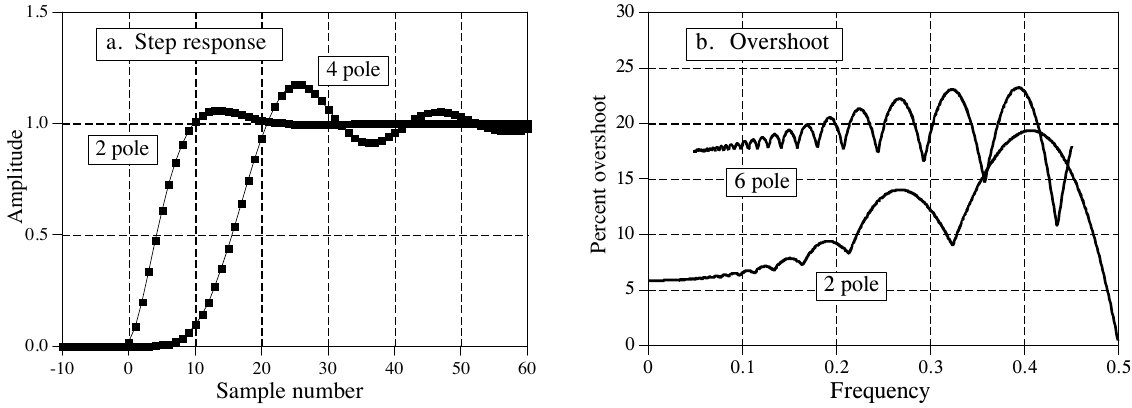
\includegraphics[width=0.943\linewidth,height=0.8\textheight,keepaspectratio]{assets/ch20/fig20-03.png}
\caption*{\textbf{图 20-3　切比雪夫阶跃响应。} 切比雪夫滤波器阶跃响应的过冲在 5\%
到 30\% 之间，取决于极点数（见 (a)）和截止频率（见 (b)）。图 (a)
的截止频率为 0.05，可以按比例换算到其他截止频率。 （a. Step response =
阶跃响应；b. Overshoot = 过冲。Amplitude = 幅度，Sample number =
采样序号，Percent overshoot = 过冲百分比，Frequency = 频率；``2 pole'' =
2 极点，``4 pole'' = 4 极点，``6 pole'' = 6 极点。）}
\end{figure}

\begin{quote}
\textbf{译注：} 用本章的 C 程序（纹波 0.5\%、\(f_C = 0.05\)）实测：2
极点过冲 6.0\%，在第 5 个采样升到 50\%，与图 (a) 中的 ``2 pole''
曲线吻合；4 极点过冲 13.9\%，在第 10 个采样升到 50\%；6 极点过冲
17.7\%，在第 16 个采样升到 50\%、第 26 个采样达到峰值。图 (a) 中标 ``4
pole'' 的那条曲线约在第 16 个采样过 50\%、峰值约 1.17，与 6
极点的实测结果吻合，与 4 极点的不符，所以这个标签很可能应为 ``6
pole''（图 (b) 画的也正是 2 极点和 6 极点）。这只是根据数值比对的推测。
\end{quote}

\section{稳定性}

用卷积实现的数字滤波器，主要限制是执行时间：只要你愿意等，几乎任何滤波器响应都能做到。递归滤波器正好相反：它们快如闪电，但性能有限。例如，考虑一个
6 极点、纹波 0.5\%、截止频率 0.01 的低通滤波器。它的递归系数可以从表
20-1 中查到：

{\def\LTcaptype{none} % do not increment counter
\begin{longtable}[]{@{}lll@{}}
\toprule\noalign{}
& a & b \\
\midrule\noalign{}
\endhead
\bottomrule\noalign{}
\endlastfoot
0 & 1.391351e-10 & \\
1 & 8.348109e-10 & 5.883343 \\
2 & 2.087027e-9 & −1.442798e+1 \\
3 & 2.782703e-9 & 1.887786e+1 \\
4 & 2.087027e-9 & −1.389914e+1 \\
5 & 8.348109e-10 & 5.459909 \\
6 & 1.391351e-10 & −8.939932e-1 \\
\end{longtable}
}

仔细看这些系数。``b''
系数的绝对值大约是十。用单精度时，每个数的舍入噪声大约是数值本身的一千万分之一，即
\(10^{-6}\) 量级。再看 ``a'' 系数，数值大约是
\(10^{-9}\)。显然出问题了：来自输入信号（经由 ``a''
系数）的贡献，会比来自之前算出的输出信号（经由 ``b'' 系数）的噪声小 1000
倍。这个滤波器没法工作！简而言之，舍入噪声限制了滤波器能用的极点数。实际数字还会稍微取决于纹波大小，以及是高通还是低通滤波器。单精度下的大致数字是：

\textbf{表 20-3　单精度下的最大极点数}

\begingroup\scriptsize\setlength{\tabcolsep}{3pt}

{\def\LTcaptype{none} % do not increment counter
\begin{longtable}[]{@{}llllllll@{}}
\toprule\noalign{}
截止频率 & 0.02 & 0.05 & 0.10 & 0.25 & 0.40 & 0.45 & 0.48 \\
\midrule\noalign{}
\endhead
\bottomrule\noalign{}
\endlastfoot
最大极点数 & 4 & 6 & 10 & 20 & 10 & 6 & 4 \\
\end{longtable}
}

\endgroup

接近这个极限时，滤波器的性能就开始变差：阶跃响应的过冲变大，阻带衰减变差，频率响应的纹波过大。如果把滤波器推得太过头，或者系数有错，输出很可能会一直振荡，直到溢出。

有两种方法可以提高能用的最大极点数。第一，使用双精度。这要求系数计算也用双精度（包括
π 的值）。

第二种方法是分级实现滤波器。例如，一个六极点滤波器原本就是三个两极点级的级联(cascade)。表
20-4
的程序把这三级合成一组递归系数，以便编程。然而，如果按原来分开的三级来实现，滤波器会更稳定。这需要知道每一级的
``a'' 和 ``b'' 系数，这些可以从表 20-4 的程序中得到：表 20-5
中的子程序对级联中的每一级各调用一次，例如对六极点滤波器调用三次。子程序结束时，有五个变量返回主程序：A0、A1、A2、B1
和
B2。它们就是正在处理的那个两极点级的递归系数，可以用来分级实现滤波器。

\textbf{表 20-4}（主程序，注释已译成中文）

\begin{Shaded}
\begin{Highlighting}[]
\NormalTok{100 \textquotesingle{}CHEBYSHEV FILTER{-} RECURSION COEFFICIENT CALCULATION}
\NormalTok{110 \textquotesingle{}}
\NormalTok{120                         \textquotesingle{}初始化变量}
\NormalTok{130 DIM A[22]               \textquotesingle{}程序结束时存放 "a" 系数}
\NormalTok{140 DIM B[22]               \textquotesingle{}程序结束时存放 "b" 系数}
\NormalTok{150 DIM TA[22]              \textquotesingle{}内部使用，用于合并各级}
\NormalTok{160 DIM TB[22]              \textquotesingle{}内部使用，用于合并各级}
\NormalTok{170 \textquotesingle{}}
\NormalTok{180 FOR I\% = 0 TO 22}
\NormalTok{190 A[I\%] = 0}
\NormalTok{200 B[I\%] = 0}
\NormalTok{210 NEXT I\%}
\NormalTok{220 \textquotesingle{}}
\NormalTok{230 A[2] = 1}
\NormalTok{240 B[2] = 1}
\NormalTok{250 PI = 3.14159265}
\NormalTok{260                         \textquotesingle{}输入四个滤波器参数}
\NormalTok{270 INPUT "Enter cutoff frequency (0 to .5): ", FC}
\NormalTok{280 INPUT "Enter 0 for LP, 1 for HP filter: ", LH}
\NormalTok{290 INPUT "Enter percent ripple (0 to 29): ", PR}
\NormalTok{300 INPUT "Enter number of poles (2,4,...20): ", NP}
\NormalTok{310 \textquotesingle{}}
\NormalTok{320 FOR P\% = 1 TO NP/2      \textquotesingle{}每个极点对循环一次}
\NormalTok{330 \textquotesingle{}}
\NormalTok{340 GOSUB 1000              \textquotesingle{}表 20{-}5 中的子程序}
\NormalTok{350 \textquotesingle{}}
\NormalTok{360 FOR I\% = 0 TO 22        \textquotesingle{}把这一级的系数加进级联}
\NormalTok{370 TA[I\%] = A[I\%]}
\NormalTok{380 TB[I\%] = B[I\%]}
\NormalTok{390 NEXT I\%}
\NormalTok{400 \textquotesingle{}}
\NormalTok{410 FOR I\% = 2 TO 22}
\NormalTok{420 A[I\%] = A0*TA[I\%] + A1*TA[I\%{-}1] + A2*TA[I\%{-}2]}
\NormalTok{430 B[I\%] =    TB[I\%] {-} B1*TB[I\%{-}1] {-} B2*TB[I\%{-}2]}
\NormalTok{440 NEXT I\%}
\NormalTok{450 \textquotesingle{}}
\NormalTok{460 NEXT P\%}
\NormalTok{470 \textquotesingle{}}
\NormalTok{480 B[2] = 0                \textquotesingle{}完成系数合并}
\NormalTok{490 FOR I\% = 0 TO 20}
\NormalTok{500 A[I\%] = A[I\%+2]}
\NormalTok{510 B[I\%] = {-}B[I\%+2]}
\NormalTok{520 NEXT I\%}
\NormalTok{530 \textquotesingle{}}
\NormalTok{540 SA = 0                  \textquotesingle{}归一化增益}
\NormalTok{550 SB = 0}
\NormalTok{560 FOR I\% = 0 TO 20}
\NormalTok{570 IF LH = 0 THEN SA = SA + A[I\%]}
\NormalTok{580 IF LH = 0 THEN SB = SB + B[I\%]}
\NormalTok{590 IF LH = 1 THEN SA = SA + A[I\%] * ({-}1)\^{}I\%}
\NormalTok{600 IF LH = 1 THEN SB = SB + B[I\%] * ({-}1)\^{}I\%}
\NormalTok{610 NEXT I\%}
\NormalTok{620 \textquotesingle{}}
\NormalTok{630 GAIN = SA / (1 {-} SB)}
\NormalTok{640 \textquotesingle{}}
\NormalTok{650 FOR I\% = 0 TO 20}
\NormalTok{660 A[I\%] = A[I\%] / GAIN}
\NormalTok{670 NEXT I\%}
\NormalTok{680 \textquotesingle{}                       \textquotesingle{}最终的递归系数在 A[ ] 和 B[ ] 中}
\NormalTok{690 END}
\end{Highlighting}
\end{Shaded}

\textbf{表 20-5}（子程序，注释已译成中文）

\begin{Shaded}
\begin{Highlighting}[]
\NormalTok{1000 \textquotesingle{}THIS SUBROUTINE IS CALLED FROM TABLE 20{-}4, LINE 340}
\NormalTok{1010 \textquotesingle{}}
\NormalTok{1020 \textquotesingle{} 进入子程序的变量：   PI, FC, LH, PR, HP, P\%}
\NormalTok{1030 \textquotesingle{} 离开子程序的变量：   A0, A1, A2, B1, B2}
\NormalTok{1040 \textquotesingle{} 内部使用的变量：     RP, IP, ES, VX, KX, T, W, M, D, K,}
\NormalTok{1050 \textquotesingle{}                      X0, X1, X2, Y1, Y2}
\NormalTok{1060 \textquotesingle{}}
\NormalTok{1070 \textquotesingle{}                      \textquotesingle{}计算极点在单位圆上的位置}
\NormalTok{1080 RP = {-}COS(PI/(NP*2) + (P\%{-}1) * PI/NP)}
\NormalTok{1090 IP = SIN(PI/(NP*2) + (P\%{-}1) * PI/NP)}
\NormalTok{1100 \textquotesingle{}}
\NormalTok{1110 \textquotesingle{}                      \textquotesingle{}把圆压成椭圆}
\NormalTok{1120 IF PR = 0 THEN GOTO 1210}
\NormalTok{1130 ES = SQR( (100 / (100{-}PR))\^{}2 {-}1 )}
\NormalTok{1140 VX = (1/NP) * LOG( (1/ES) + SQR( (1/ES\^{}2) + 1) )}
\NormalTok{1150 KX = (1/NP) * LOG( (1/ES) + SQR( (1/ES\^{}2) {-} 1) )}
\NormalTok{1160 KX = (EXP(KX) + EXP({-}KX))/2}
\NormalTok{1170 RP = RP * ( (EXP(VX) {-} EXP({-}VX) ) /2 ) / KX}
\NormalTok{1180 IP = IP * ( (EXP(VX) + EXP({-}VX) ) /2 ) / KX}
\NormalTok{1190 \textquotesingle{}}
\NormalTok{1200 \textquotesingle{}                      \textquotesingle{}s 域到 z 域的转换}
\NormalTok{1210 T = 2 * TAN(1/2)}
\NormalTok{1220 W = 2*PI*FC}
\NormalTok{1230 M = RP\^{}2 + IP\^{}2}
\NormalTok{1240 D = 4 {-} 4*RP*T + M*T\^{}2}
\NormalTok{1250 X0 = T\^{}2/D}
\NormalTok{1260 X1 = 2*T\^{}2/D}
\NormalTok{1270 X2 = T\^{}2/D}
\NormalTok{1280 Y1 = (8 {-} 2*M*T\^{}2)/D}
\NormalTok{1290 Y2 = ({-}4 {-} 4*RP*T {-} M*T\^{}2)/D}
\NormalTok{1300 \textquotesingle{}}
\NormalTok{1310 \textquotesingle{}                      \textquotesingle{}低通到低通，或低通到高通的变换}
\NormalTok{1320 IF LH = 1 THEN K = {-}COS(W/2 + 1/2) / COS(W/2 {-} 1/2)}
\NormalTok{1330 IF LH = 0 THEN K = SIN(1/2 {-} W/2) / SIN(1/2 + W/2)}
\NormalTok{1340 D = 1 + Y1*K {-} Y2*K\^{}2}
\NormalTok{1350 A0 = (X0 {-} X1*K + X2*K\^{}2)/D}
\NormalTok{1360 A1 = ({-}2*X0*K + X1 + X1*K\^{}2 {-} 2*X2*K)/D}
\NormalTok{1370 A2 = (X0*K\^{}2 {-} X1*K + X2)/D}
\NormalTok{1380 B1 = (2*K + Y1 + Y1*K\^{}2 {-} 2*Y2*K)/D}
\NormalTok{1390 B2 = ({-}(K\^{}2) {-} Y1*K + Y2)/D}
\NormalTok{1400 IF LH = 1 THEN A1 = {-}A1}
\NormalTok{1410 IF LH = 1 THEN B1 = {-}B1}
\NormalTok{1420 \textquotesingle{}}
\NormalTok{1430 RETURN}
\end{Highlighting}
\end{Shaded}

\textbf{表 20-4 和 20-5 的说明：} 计算切比雪夫递归滤波器 ``a'' 和 ``b''
系数的程序。第 270～300 行输入四个参数。截止频率 FC
以采样频率的分数表示，因此必须在 0 到 0.5 之间。变量 LH 设为 1
表示高通滤波器，设为 0 表示低通滤波器。PR 的取值必须在 0 到 29
之间，对应滤波器频率响应中 0 到 29\% 的纹波。滤波器的极点数存放在变量 NP
中，必须是 2 到 20 之间的偶数。程序结束时，``a'' 和 ``b'' 系数存放在数组
A{[} {]} 和 B{[} {]} 中（a0 = A{[}0{]}，a1 = A{[}1{]}，依此类推）。表
20-5 是主程序第 340
行调用的子程序。传给这个子程序六个变量，返回五个变量。表
20-6（下一页）包含两组帮助调试这个子程序的数据。函数 COS 和 SIN
使用弧度而不是角度。函数 LOG 是自然（以 e
为底的）对数。把所有浮点变量（包括 π
的值）都声明为双精度，就能使用更多的极点。表 20-1 和 20-2
就是用这个程序生成的，可以用来检验程序是否正确运行。第 33
章讲这个程序的数学原理。

\begin{quote}
\textbf{译注：} 表 20-5 第 1020 行列出的进入变量 ``HP''
是笔误，子程序实际用到的是极点数 NP（第 1080、1090、1140、1150
行），应为 ``PI, FC, LH, PR, NP, P\%''。
\end{quote}

\textbf{C 实现}（完整可编译版本见
\texttt{c/table20-4\_chebyshev\_design.c}，把表 20-4 主程序和表 20-5
子程序合成一个文件。带四个参数运行时打印系数；不带参数时运行自检）：

\begin{Shaded}
\begin{Highlighting}[]
\CommentTok{/* 表 20{-}5：计算第 p 个极点对（两极点级）的递归系数 */}
\DataTypeTok{static}\NormalTok{ Stage chebyshev\_stage}\OperatorTok{(}\DataTypeTok{double}\NormalTok{ fc}\OperatorTok{,} \DataTypeTok{int}\NormalTok{ lh}\OperatorTok{,} \DataTypeTok{double}\NormalTok{ pr}\OperatorTok{,} \DataTypeTok{int}\NormalTok{ np}\OperatorTok{,} \DataTypeTok{int}\NormalTok{ p}\OperatorTok{)}
\OperatorTok{\{}
\NormalTok{    Stage s }\OperatorTok{=} \OperatorTok{\{}\DecValTok{0}\OperatorTok{\};}
    \CommentTok{/* 1080～1090：极点在单位圆上的位置 */}
\NormalTok{    s}\OperatorTok{.}\NormalTok{rp }\OperatorTok{=} \OperatorTok{{-}}\NormalTok{cos}\OperatorTok{(}\NormalTok{PI }\OperatorTok{/} \OperatorTok{(}\NormalTok{np }\OperatorTok{*} \DecValTok{2}\OperatorTok{)} \OperatorTok{+} \OperatorTok{(}\NormalTok{p }\OperatorTok{{-}} \DecValTok{1}\OperatorTok{)} \OperatorTok{*}\NormalTok{ PI }\OperatorTok{/}\NormalTok{ np}\OperatorTok{);}
\NormalTok{    s}\OperatorTok{.}\NormalTok{ip }\OperatorTok{=}\NormalTok{  sin}\OperatorTok{(}\NormalTok{PI }\OperatorTok{/} \OperatorTok{(}\NormalTok{np }\OperatorTok{*} \DecValTok{2}\OperatorTok{)} \OperatorTok{+} \OperatorTok{(}\NormalTok{p }\OperatorTok{{-}} \DecValTok{1}\OperatorTok{)} \OperatorTok{*}\NormalTok{ PI }\OperatorTok{/}\NormalTok{ np}\OperatorTok{);}

    \CommentTok{/* 1120～1180：有纹波时，把圆压成椭圆；纹波为 0 就是巴特沃斯，跳过 */}
    \ControlFlowTok{if} \OperatorTok{(}\NormalTok{pr }\OperatorTok{!=} \DecValTok{0}\OperatorTok{)} \OperatorTok{\{}
\NormalTok{        s}\OperatorTok{.}\NormalTok{es }\OperatorTok{=}\NormalTok{ sqrt}\OperatorTok{(}\NormalTok{pow}\OperatorTok{(}\FloatTok{100.0} \OperatorTok{/} \OperatorTok{(}\FloatTok{100.0} \OperatorTok{{-}}\NormalTok{ pr}\OperatorTok{),} \DecValTok{2}\OperatorTok{)} \OperatorTok{{-}} \DecValTok{1}\OperatorTok{);}
\NormalTok{        s}\OperatorTok{.}\NormalTok{vx }\OperatorTok{=} \OperatorTok{(}\FloatTok{1.0} \OperatorTok{/}\NormalTok{ np}\OperatorTok{)} \OperatorTok{*}\NormalTok{ log}\OperatorTok{((}\DecValTok{1} \OperatorTok{/}\NormalTok{ s}\OperatorTok{.}\NormalTok{es}\OperatorTok{)} \OperatorTok{+}\NormalTok{ sqrt}\OperatorTok{((}\DecValTok{1} \OperatorTok{/} \OperatorTok{(}\NormalTok{s}\OperatorTok{.}\NormalTok{es }\OperatorTok{*}\NormalTok{ s}\OperatorTok{.}\NormalTok{es}\OperatorTok{))} \OperatorTok{+} \DecValTok{1}\OperatorTok{));}
\NormalTok{        s}\OperatorTok{.}\NormalTok{kx }\OperatorTok{=} \OperatorTok{(}\FloatTok{1.0} \OperatorTok{/}\NormalTok{ np}\OperatorTok{)} \OperatorTok{*}\NormalTok{ log}\OperatorTok{((}\DecValTok{1} \OperatorTok{/}\NormalTok{ s}\OperatorTok{.}\NormalTok{es}\OperatorTok{)} \OperatorTok{+}\NormalTok{ sqrt}\OperatorTok{((}\DecValTok{1} \OperatorTok{/} \OperatorTok{(}\NormalTok{s}\OperatorTok{.}\NormalTok{es }\OperatorTok{*}\NormalTok{ s}\OperatorTok{.}\NormalTok{es}\OperatorTok{))} \OperatorTok{{-}} \DecValTok{1}\OperatorTok{));}
\NormalTok{        s}\OperatorTok{.}\NormalTok{kx }\OperatorTok{=} \OperatorTok{(}\NormalTok{exp}\OperatorTok{(}\NormalTok{s}\OperatorTok{.}\NormalTok{kx}\OperatorTok{)} \OperatorTok{+}\NormalTok{ exp}\OperatorTok{({-}}\NormalTok{s}\OperatorTok{.}\NormalTok{kx}\OperatorTok{))} \OperatorTok{/} \DecValTok{2}\OperatorTok{;}
\NormalTok{        s}\OperatorTok{.}\NormalTok{rp }\OperatorTok{=}\NormalTok{ s}\OperatorTok{.}\NormalTok{rp }\OperatorTok{*} \OperatorTok{((}\NormalTok{exp}\OperatorTok{(}\NormalTok{s}\OperatorTok{.}\NormalTok{vx}\OperatorTok{)} \OperatorTok{{-}}\NormalTok{ exp}\OperatorTok{({-}}\NormalTok{s}\OperatorTok{.}\NormalTok{vx}\OperatorTok{))} \OperatorTok{/} \DecValTok{2}\OperatorTok{)} \OperatorTok{/}\NormalTok{ s}\OperatorTok{.}\NormalTok{kx}\OperatorTok{;}
\NormalTok{        s}\OperatorTok{.}\NormalTok{ip }\OperatorTok{=}\NormalTok{ s}\OperatorTok{.}\NormalTok{ip }\OperatorTok{*} \OperatorTok{((}\NormalTok{exp}\OperatorTok{(}\NormalTok{s}\OperatorTok{.}\NormalTok{vx}\OperatorTok{)} \OperatorTok{+}\NormalTok{ exp}\OperatorTok{({-}}\NormalTok{s}\OperatorTok{.}\NormalTok{vx}\OperatorTok{))} \OperatorTok{/} \DecValTok{2}\OperatorTok{)} \OperatorTok{/}\NormalTok{ s}\OperatorTok{.}\NormalTok{kx}\OperatorTok{;}
    \OperatorTok{\}}

    \CommentTok{/* 1210～1290：s 域到 z 域的转换 */}
\NormalTok{    s}\OperatorTok{.}\NormalTok{t  }\OperatorTok{=} \DecValTok{2} \OperatorTok{*}\NormalTok{ tan}\OperatorTok{(}\FloatTok{0.5}\OperatorTok{);}
\NormalTok{    s}\OperatorTok{.}\NormalTok{w  }\OperatorTok{=} \DecValTok{2} \OperatorTok{*}\NormalTok{ PI }\OperatorTok{*}\NormalTok{ fc}\OperatorTok{;}
\NormalTok{    s}\OperatorTok{.}\NormalTok{m  }\OperatorTok{=}\NormalTok{ s}\OperatorTok{.}\NormalTok{rp }\OperatorTok{*}\NormalTok{ s}\OperatorTok{.}\NormalTok{rp }\OperatorTok{+}\NormalTok{ s}\OperatorTok{.}\NormalTok{ip }\OperatorTok{*}\NormalTok{ s}\OperatorTok{.}\NormalTok{ip}\OperatorTok{;}
\NormalTok{    s}\OperatorTok{.}\NormalTok{d  }\OperatorTok{=} \DecValTok{4} \OperatorTok{{-}} \DecValTok{4} \OperatorTok{*}\NormalTok{ s}\OperatorTok{.}\NormalTok{rp }\OperatorTok{*}\NormalTok{ s}\OperatorTok{.}\NormalTok{t }\OperatorTok{+}\NormalTok{ s}\OperatorTok{.}\NormalTok{m }\OperatorTok{*}\NormalTok{ s}\OperatorTok{.}\NormalTok{t }\OperatorTok{*}\NormalTok{ s}\OperatorTok{.}\NormalTok{t}\OperatorTok{;}
\NormalTok{    s}\OperatorTok{.}\NormalTok{x0 }\OperatorTok{=}\NormalTok{ s}\OperatorTok{.}\NormalTok{t }\OperatorTok{*}\NormalTok{ s}\OperatorTok{.}\NormalTok{t }\OperatorTok{/}\NormalTok{ s}\OperatorTok{.}\NormalTok{d}\OperatorTok{;}
\NormalTok{    s}\OperatorTok{.}\NormalTok{x1 }\OperatorTok{=} \DecValTok{2} \OperatorTok{*}\NormalTok{ s}\OperatorTok{.}\NormalTok{t }\OperatorTok{*}\NormalTok{ s}\OperatorTok{.}\NormalTok{t }\OperatorTok{/}\NormalTok{ s}\OperatorTok{.}\NormalTok{d}\OperatorTok{;}
\NormalTok{    s}\OperatorTok{.}\NormalTok{x2 }\OperatorTok{=}\NormalTok{ s}\OperatorTok{.}\NormalTok{t }\OperatorTok{*}\NormalTok{ s}\OperatorTok{.}\NormalTok{t }\OperatorTok{/}\NormalTok{ s}\OperatorTok{.}\NormalTok{d}\OperatorTok{;}
\NormalTok{    s}\OperatorTok{.}\NormalTok{y1 }\OperatorTok{=} \OperatorTok{(}\DecValTok{8} \OperatorTok{{-}} \DecValTok{2} \OperatorTok{*}\NormalTok{ s}\OperatorTok{.}\NormalTok{m }\OperatorTok{*}\NormalTok{ s}\OperatorTok{.}\NormalTok{t }\OperatorTok{*}\NormalTok{ s}\OperatorTok{.}\NormalTok{t}\OperatorTok{)} \OperatorTok{/}\NormalTok{ s}\OperatorTok{.}\NormalTok{d}\OperatorTok{;}
\NormalTok{    s}\OperatorTok{.}\NormalTok{y2 }\OperatorTok{=} \OperatorTok{({-}}\DecValTok{4} \OperatorTok{{-}} \DecValTok{4} \OperatorTok{*}\NormalTok{ s}\OperatorTok{.}\NormalTok{rp }\OperatorTok{*}\NormalTok{ s}\OperatorTok{.}\NormalTok{t }\OperatorTok{{-}}\NormalTok{ s}\OperatorTok{.}\NormalTok{m }\OperatorTok{*}\NormalTok{ s}\OperatorTok{.}\NormalTok{t }\OperatorTok{*}\NormalTok{ s}\OperatorTok{.}\NormalTok{t}\OperatorTok{)} \OperatorTok{/}\NormalTok{ s}\OperatorTok{.}\NormalTok{d}\OperatorTok{;}

    \CommentTok{/* 1320～1410：低通到低通，或低通到高通的变换 */}
    \DataTypeTok{double}\NormalTok{ k }\OperatorTok{=}\NormalTok{ lh }\OperatorTok{?} \OperatorTok{{-}}\NormalTok{cos}\OperatorTok{(}\NormalTok{s}\OperatorTok{.}\NormalTok{w }\OperatorTok{/} \DecValTok{2} \OperatorTok{+} \FloatTok{0.5}\OperatorTok{)} \OperatorTok{/}\NormalTok{ cos}\OperatorTok{(}\NormalTok{s}\OperatorTok{.}\NormalTok{w }\OperatorTok{/} \DecValTok{2} \OperatorTok{{-}} \FloatTok{0.5}\OperatorTok{)}
                  \OperatorTok{:}\NormalTok{  sin}\OperatorTok{(}\FloatTok{0.5} \OperatorTok{{-}}\NormalTok{ s}\OperatorTok{.}\NormalTok{w }\OperatorTok{/} \DecValTok{2}\OperatorTok{)} \OperatorTok{/}\NormalTok{ sin}\OperatorTok{(}\FloatTok{0.5} \OperatorTok{+}\NormalTok{ s}\OperatorTok{.}\NormalTok{w }\OperatorTok{/} \DecValTok{2}\OperatorTok{);}
    \DataTypeTok{double}\NormalTok{ d }\OperatorTok{=} \DecValTok{1} \OperatorTok{+}\NormalTok{ s}\OperatorTok{.}\NormalTok{y1 }\OperatorTok{*}\NormalTok{ k }\OperatorTok{{-}}\NormalTok{ s}\OperatorTok{.}\NormalTok{y2 }\OperatorTok{*}\NormalTok{ k }\OperatorTok{*}\NormalTok{ k}\OperatorTok{;}
\NormalTok{    s}\OperatorTok{.}\NormalTok{a0 }\OperatorTok{=} \OperatorTok{(}\NormalTok{s}\OperatorTok{.}\NormalTok{x0 }\OperatorTok{{-}}\NormalTok{ s}\OperatorTok{.}\NormalTok{x1 }\OperatorTok{*}\NormalTok{ k }\OperatorTok{+}\NormalTok{ s}\OperatorTok{.}\NormalTok{x2 }\OperatorTok{*}\NormalTok{ k }\OperatorTok{*}\NormalTok{ k}\OperatorTok{)} \OperatorTok{/}\NormalTok{ d}\OperatorTok{;}
\NormalTok{    s}\OperatorTok{.}\NormalTok{a1 }\OperatorTok{=} \OperatorTok{({-}}\DecValTok{2} \OperatorTok{*}\NormalTok{ s}\OperatorTok{.}\NormalTok{x0 }\OperatorTok{*}\NormalTok{ k }\OperatorTok{+}\NormalTok{ s}\OperatorTok{.}\NormalTok{x1 }\OperatorTok{+}\NormalTok{ s}\OperatorTok{.}\NormalTok{x1 }\OperatorTok{*}\NormalTok{ k }\OperatorTok{*}\NormalTok{ k }\OperatorTok{{-}} \DecValTok{2} \OperatorTok{*}\NormalTok{ s}\OperatorTok{.}\NormalTok{x2 }\OperatorTok{*}\NormalTok{ k}\OperatorTok{)} \OperatorTok{/}\NormalTok{ d}\OperatorTok{;}
\NormalTok{    s}\OperatorTok{.}\NormalTok{a2 }\OperatorTok{=} \OperatorTok{(}\NormalTok{s}\OperatorTok{.}\NormalTok{x0 }\OperatorTok{*}\NormalTok{ k }\OperatorTok{*}\NormalTok{ k }\OperatorTok{{-}}\NormalTok{ s}\OperatorTok{.}\NormalTok{x1 }\OperatorTok{*}\NormalTok{ k }\OperatorTok{+}\NormalTok{ s}\OperatorTok{.}\NormalTok{x2}\OperatorTok{)} \OperatorTok{/}\NormalTok{ d}\OperatorTok{;}
\NormalTok{    s}\OperatorTok{.}\NormalTok{b1 }\OperatorTok{=} \OperatorTok{(}\DecValTok{2} \OperatorTok{*}\NormalTok{ k }\OperatorTok{+}\NormalTok{ s}\OperatorTok{.}\NormalTok{y1 }\OperatorTok{+}\NormalTok{ s}\OperatorTok{.}\NormalTok{y1 }\OperatorTok{*}\NormalTok{ k }\OperatorTok{*}\NormalTok{ k }\OperatorTok{{-}} \DecValTok{2} \OperatorTok{*}\NormalTok{ s}\OperatorTok{.}\NormalTok{y2 }\OperatorTok{*}\NormalTok{ k}\OperatorTok{)} \OperatorTok{/}\NormalTok{ d}\OperatorTok{;}
\NormalTok{    s}\OperatorTok{.}\NormalTok{b2 }\OperatorTok{=} \OperatorTok{({-}(}\NormalTok{k }\OperatorTok{*}\NormalTok{ k}\OperatorTok{)} \OperatorTok{{-}}\NormalTok{ s}\OperatorTok{.}\NormalTok{y1 }\OperatorTok{*}\NormalTok{ k }\OperatorTok{+}\NormalTok{ s}\OperatorTok{.}\NormalTok{y2}\OperatorTok{)} \OperatorTok{/}\NormalTok{ d}\OperatorTok{;}
    \ControlFlowTok{if} \OperatorTok{(}\NormalTok{lh}\OperatorTok{)} \OperatorTok{\{}\NormalTok{ s}\OperatorTok{.}\NormalTok{a1 }\OperatorTok{=} \OperatorTok{{-}}\NormalTok{s}\OperatorTok{.}\NormalTok{a1}\OperatorTok{;}\NormalTok{ s}\OperatorTok{.}\NormalTok{b1 }\OperatorTok{=} \OperatorTok{{-}}\NormalTok{s}\OperatorTok{.}\NormalTok{b1}\OperatorTok{;} \OperatorTok{\}}
    \ControlFlowTok{return}\NormalTok{ s}\OperatorTok{;}
\OperatorTok{\}}

\CommentTok{/* 表 20{-}4：把 np/2 个两极点级合成一组递归系数，结果 a[0..np]、b[1..np] */}
\DataTypeTok{static} \DataTypeTok{void}\NormalTok{ chebyshev\_design}\OperatorTok{(}\DataTypeTok{double}\NormalTok{ fc}\OperatorTok{,} \DataTypeTok{int}\NormalTok{ lh}\OperatorTok{,} \DataTypeTok{double}\NormalTok{ pr}\OperatorTok{,} \DataTypeTok{int}\NormalTok{ np}\OperatorTok{,} \DataTypeTok{double} \OperatorTok{*}\NormalTok{a}\OperatorTok{,} \DataTypeTok{double} \OperatorTok{*}\NormalTok{b}\OperatorTok{)}
\OperatorTok{\{}
    \DataTypeTok{double}\NormalTok{ ta}\OperatorTok{[}\NormalTok{NC}\OperatorTok{],}\NormalTok{ tb}\OperatorTok{[}\NormalTok{NC}\OperatorTok{];}
    \ControlFlowTok{for} \OperatorTok{(}\DataTypeTok{int}\NormalTok{ i }\OperatorTok{=} \DecValTok{0}\OperatorTok{;}\NormalTok{ i }\OperatorTok{\textless{}}\NormalTok{ NC}\OperatorTok{;}\NormalTok{ i}\OperatorTok{++)}\NormalTok{ a}\OperatorTok{[}\NormalTok{i}\OperatorTok{]} \OperatorTok{=}\NormalTok{ b}\OperatorTok{[}\NormalTok{i}\OperatorTok{]} \OperatorTok{=} \DecValTok{0}\OperatorTok{;}    \CommentTok{/* 180～210 */}
\NormalTok{    a}\OperatorTok{[}\DecValTok{2}\OperatorTok{]} \OperatorTok{=} \DecValTok{1}\OperatorTok{;}                                        \CommentTok{/* 230～240：从 1 开始做多项式乘法 */}
\NormalTok{    b}\OperatorTok{[}\DecValTok{2}\OperatorTok{]} \OperatorTok{=} \DecValTok{1}\OperatorTok{;}

    \ControlFlowTok{for} \OperatorTok{(}\DataTypeTok{int}\NormalTok{ p }\OperatorTok{=} \DecValTok{1}\OperatorTok{;}\NormalTok{ p }\OperatorTok{\textless{}=}\NormalTok{ np }\OperatorTok{/} \DecValTok{2}\OperatorTok{;}\NormalTok{ p}\OperatorTok{++)} \OperatorTok{\{}              \CommentTok{/* 320：每个极点对循环一次 */}
\NormalTok{        Stage s }\OperatorTok{=}\NormalTok{ chebyshev\_stage}\OperatorTok{(}\NormalTok{fc}\OperatorTok{,}\NormalTok{ lh}\OperatorTok{,}\NormalTok{ pr}\OperatorTok{,}\NormalTok{ np}\OperatorTok{,}\NormalTok{ p}\OperatorTok{);}    \CommentTok{/* 340：GOSUB 1000 */}
        \ControlFlowTok{for} \OperatorTok{(}\DataTypeTok{int}\NormalTok{ i }\OperatorTok{=} \DecValTok{0}\OperatorTok{;}\NormalTok{ i }\OperatorTok{\textless{}}\NormalTok{ NC}\OperatorTok{;}\NormalTok{ i}\OperatorTok{++)} \OperatorTok{\{}\NormalTok{ ta}\OperatorTok{[}\NormalTok{i}\OperatorTok{]} \OperatorTok{=}\NormalTok{ a}\OperatorTok{[}\NormalTok{i}\OperatorTok{];}\NormalTok{ tb}\OperatorTok{[}\NormalTok{i}\OperatorTok{]} \OperatorTok{=}\NormalTok{ b}\OperatorTok{[}\NormalTok{i}\OperatorTok{];} \OperatorTok{\}}   \CommentTok{/* 360～390 */}
        \ControlFlowTok{for} \OperatorTok{(}\DataTypeTok{int}\NormalTok{ i }\OperatorTok{=} \DecValTok{2}\OperatorTok{;}\NormalTok{ i }\OperatorTok{\textless{}}\NormalTok{ NC}\OperatorTok{;}\NormalTok{ i}\OperatorTok{++)} \OperatorTok{\{}               \CommentTok{/* 410～440：把这一级串进级联 */}
\NormalTok{            a}\OperatorTok{[}\NormalTok{i}\OperatorTok{]} \OperatorTok{=}\NormalTok{ s}\OperatorTok{.}\NormalTok{a0 }\OperatorTok{*}\NormalTok{ ta}\OperatorTok{[}\NormalTok{i}\OperatorTok{]} \OperatorTok{+}\NormalTok{ s}\OperatorTok{.}\NormalTok{a1 }\OperatorTok{*}\NormalTok{ ta}\OperatorTok{[}\NormalTok{i }\OperatorTok{{-}} \DecValTok{1}\OperatorTok{]} \OperatorTok{+}\NormalTok{ s}\OperatorTok{.}\NormalTok{a2 }\OperatorTok{*}\NormalTok{ ta}\OperatorTok{[}\NormalTok{i }\OperatorTok{{-}} \DecValTok{2}\OperatorTok{];}
\NormalTok{            b}\OperatorTok{[}\NormalTok{i}\OperatorTok{]} \OperatorTok{=}\NormalTok{        tb}\OperatorTok{[}\NormalTok{i}\OperatorTok{]} \OperatorTok{{-}}\NormalTok{ s}\OperatorTok{.}\NormalTok{b1 }\OperatorTok{*}\NormalTok{ tb}\OperatorTok{[}\NormalTok{i }\OperatorTok{{-}} \DecValTok{1}\OperatorTok{]} \OperatorTok{{-}}\NormalTok{ s}\OperatorTok{.}\NormalTok{b2 }\OperatorTok{*}\NormalTok{ tb}\OperatorTok{[}\NormalTok{i }\OperatorTok{{-}} \DecValTok{2}\OperatorTok{];}
        \OperatorTok{\}}
    \OperatorTok{\}}

\NormalTok{    b}\OperatorTok{[}\DecValTok{2}\OperatorTok{]} \OperatorTok{=} \DecValTok{0}\OperatorTok{;}                                        \CommentTok{/* 480～520：收尾，下标左移 2 位，b 取反 */}
    \ControlFlowTok{for} \OperatorTok{(}\DataTypeTok{int}\NormalTok{ i }\OperatorTok{=} \DecValTok{0}\OperatorTok{;}\NormalTok{ i }\OperatorTok{\textless{}=} \DecValTok{20}\OperatorTok{;}\NormalTok{ i}\OperatorTok{++)} \OperatorTok{\{}\NormalTok{ a}\OperatorTok{[}\NormalTok{i}\OperatorTok{]} \OperatorTok{=}\NormalTok{ a}\OperatorTok{[}\NormalTok{i }\OperatorTok{+} \DecValTok{2}\OperatorTok{];}\NormalTok{ b}\OperatorTok{[}\NormalTok{i}\OperatorTok{]} \OperatorTok{=} \OperatorTok{{-}}\NormalTok{b}\OperatorTok{[}\NormalTok{i }\OperatorTok{+} \DecValTok{2}\OperatorTok{];} \OperatorTok{\}}

    \DataTypeTok{double}\NormalTok{ sa }\OperatorTok{=} \DecValTok{0}\OperatorTok{,}\NormalTok{ sb }\OperatorTok{=} \DecValTok{0}\OperatorTok{;}                           \CommentTok{/* 540～610：归一化增益 */}
    \ControlFlowTok{for} \OperatorTok{(}\DataTypeTok{int}\NormalTok{ i }\OperatorTok{=} \DecValTok{0}\OperatorTok{;}\NormalTok{ i }\OperatorTok{\textless{}=} \DecValTok{20}\OperatorTok{;}\NormalTok{ i}\OperatorTok{++)} \OperatorTok{\{}
        \DataTypeTok{double}\NormalTok{ sign }\OperatorTok{=} \OperatorTok{(}\NormalTok{lh }\OperatorTok{\&\&} \OperatorTok{(}\NormalTok{i }\OperatorTok{\&} \DecValTok{1}\OperatorTok{))} \OperatorTok{?} \OperatorTok{{-}}\FloatTok{1.0} \OperatorTok{:} \FloatTok{1.0}\OperatorTok{;}  \CommentTok{/* 高通在 0.5 处归一化，乘 ({-}1)\^{}i */}
\NormalTok{        sa }\OperatorTok{+=}\NormalTok{ a}\OperatorTok{[}\NormalTok{i}\OperatorTok{]} \OperatorTok{*}\NormalTok{ sign}\OperatorTok{;}
\NormalTok{        sb }\OperatorTok{+=}\NormalTok{ b}\OperatorTok{[}\NormalTok{i}\OperatorTok{]} \OperatorTok{*}\NormalTok{ sign}\OperatorTok{;}
    \OperatorTok{\}}
    \DataTypeTok{double}\NormalTok{ gain }\OperatorTok{=}\NormalTok{ sa }\OperatorTok{/} \OperatorTok{(}\DecValTok{1} \OperatorTok{{-}}\NormalTok{ sb}\OperatorTok{);}                     \CommentTok{/* 630 */}
    \ControlFlowTok{for} \OperatorTok{(}\DataTypeTok{int}\NormalTok{ i }\OperatorTok{=} \DecValTok{0}\OperatorTok{;}\NormalTok{ i }\OperatorTok{\textless{}=} \DecValTok{20}\OperatorTok{;}\NormalTok{ i}\OperatorTok{++)}\NormalTok{ a}\OperatorTok{[}\NormalTok{i}\OperatorTok{]} \OperatorTok{/=}\NormalTok{ gain}\OperatorTok{;}      \CommentTok{/* 650～670 */}
\OperatorTok{\}}
\end{Highlighting}
\end{Shaded}

运行结果（双精度）： - \textbf{对照表 20-6 的调试数据：} 两组数据各 19
个变量，与表中数值的最大差分别为 8.5×10⁻⁷ 和
8.7×10⁻⁷，即表中给出的六位小数全部吻合。 - \textbf{对照表 20-1 和
20-2：} 低通、高通各 12 个截止频率 × 3 种极点数，共 648
个系数，与原书最大相对差 2.5×10⁻⁵。 - \textbf{频率响应：} 截止频率
0.1、纹波 0.5\% 的 2、4、6 极点低通和高通滤波器，在截止频率处的幅度都是
0.7107，与''截止频率在幅度穿过 0.707 处测量''一致；通带最大值都是
1.0050，即 0.5\% 的纹波。离截止频率 0.1 处的阻带衰减：低通 2/4/6
极点分别为 −14.8、−33.8、−56.1 dB，极点越多滚降越陡，与图 20-2 一致。

\textbf{表 20-6　调试数据。} 这张表包含两组数据，用于调试表 20-5
中的子程序。

{\def\LTcaptype{none} % do not increment counter
\begin{longtable}[]{@{}lll@{}}
\toprule\noalign{}
& 数据组 1 & 数据组 2 \\
\midrule\noalign{}
\endhead
\bottomrule\noalign{}
\endlastfoot
\textbf{进入子程序时的值} & & \\
FC & 0.1 & 0.1 \\
LH & 0 & 1 \\
PR & 0 & 10 \\
NP & 4 & 4 \\
P\% & 1 & 2 \\
PI & 3.141592 & 3.141592 \\
\textbf{第 1200 行处应有的值} & & \\
RP & −0.923879 & −0.136178 \\
IP & 0.382683 & 0.933223 \\
ES & 不使用 & 0.484322 \\
VX & 不使用 & 0.368054 \\
KX & 不使用 & 1.057802 \\
\textbf{第 1310 行处应有的值} & & \\
T & 1.092605 & 1.092605 \\
W & 0.628318 & 0.628318 \\
M & 1.000000 & 0.889450 \\
D & 9.231528 & 5.656972 \\
X0 & 0.129316 & 0.211029 \\
X1 & 0.258632 & 0.422058 \\
X2 & 0.129316 & 0.211029 \\
Y1 & 0.607963 & 1.038784 \\
Y2 & −0.125227 & −0.789584 \\
\textbf{返回主程序的值} & & \\
A0 & 0.061885 & 0.922919 \\
A1 & 0.123770 & −1.845840 \\
A2 & 0.061885 & 0.922919 \\
B1 & 1.048600 & 1.446913 \\
B2 & −0.296140 & −0.836653 \\
\end{longtable}
}

% !TEX root = ../main.tex
% 本文件由 build-tex.sh 从 21-DSP指南-第21章中译.md 生成，改内容请改 md 后重新生成

\chapter{滤波器比较}\label{ch-21}

选择，选择，还是选择！有这么多滤波器可选，怎么知道该用哪一个？本章是一场滤波器之间的正面对决：我们从各方选出冠军，让它们一决高下。第一场，数字滤波器(digital
filter)对阵模拟滤波器(analog filter)，看哪种技术更强。第二轮，加窗 sinc
滤波器(windowed-sinc filter)对阵切比雪夫滤波器(Chebyshev
filter)，争夺频域滤波器之王。最后一战，移动平均滤波器(moving average
filter)与单极点滤波器(single pole
filter)争夺时域冠军。废话少说，比赛开始！

\section{第一场：模拟滤波器 vs.~数字滤波器}

大多数数字信号都源自模拟电子电路。如果信号需要滤波，是在数字化之前用模拟滤波器好，还是数字化之后用数字滤波器好？我们让两位最强的选手过过招，来回答这个问题。

目标是实现一个 1 kHz
的低通滤波器。代表模拟一方出战的，是一个纹波(ripple)为 0.5
dB（6\%）的六极点切比雪夫滤波器。如第 3 章所述，它可以用 3
个运算放大器(op amp)、12 个电阻和 6 个电容搭出来。数字一方的角落里，加窗
sinc 滤波器已经热身完毕、准备开打。模拟信号以 10 kHz
的采样率数字化，于是截止频率在数字频率刻度上是 0.1。加窗 sinc 的长度选为
129 点，使它与模拟滤波器有相同的 90\% 到 10\%
滚降(roll-off)。公平起见。图 21-1
给出了这两个滤波器的频率响应和阶跃响应。

我们来逐招比较这两个滤波器。如 (a) 和 (b)
所示，模拟滤波器的通带(passband)有 6\%
的纹波，而数字滤波器完全平坦（误差在 0.02\%
以内）。模拟设计者可能会争辩说，纹波大小在设计时可以自己选；但这没抓住要点。模拟滤波器能达到的平坦度，受限于其电阻和电容的精度。即使设计成巴特沃斯响应(Butterworth
response，即 0\% 纹波)，这种复杂度的滤波器也会残留大约 1\%
的纹波。另一方面，数字滤波器的平坦度主要受舍入误差限制，比模拟滤波器平坦几百倍。数字滤波器得一分。

\begin{figure}[htbp]
\centering
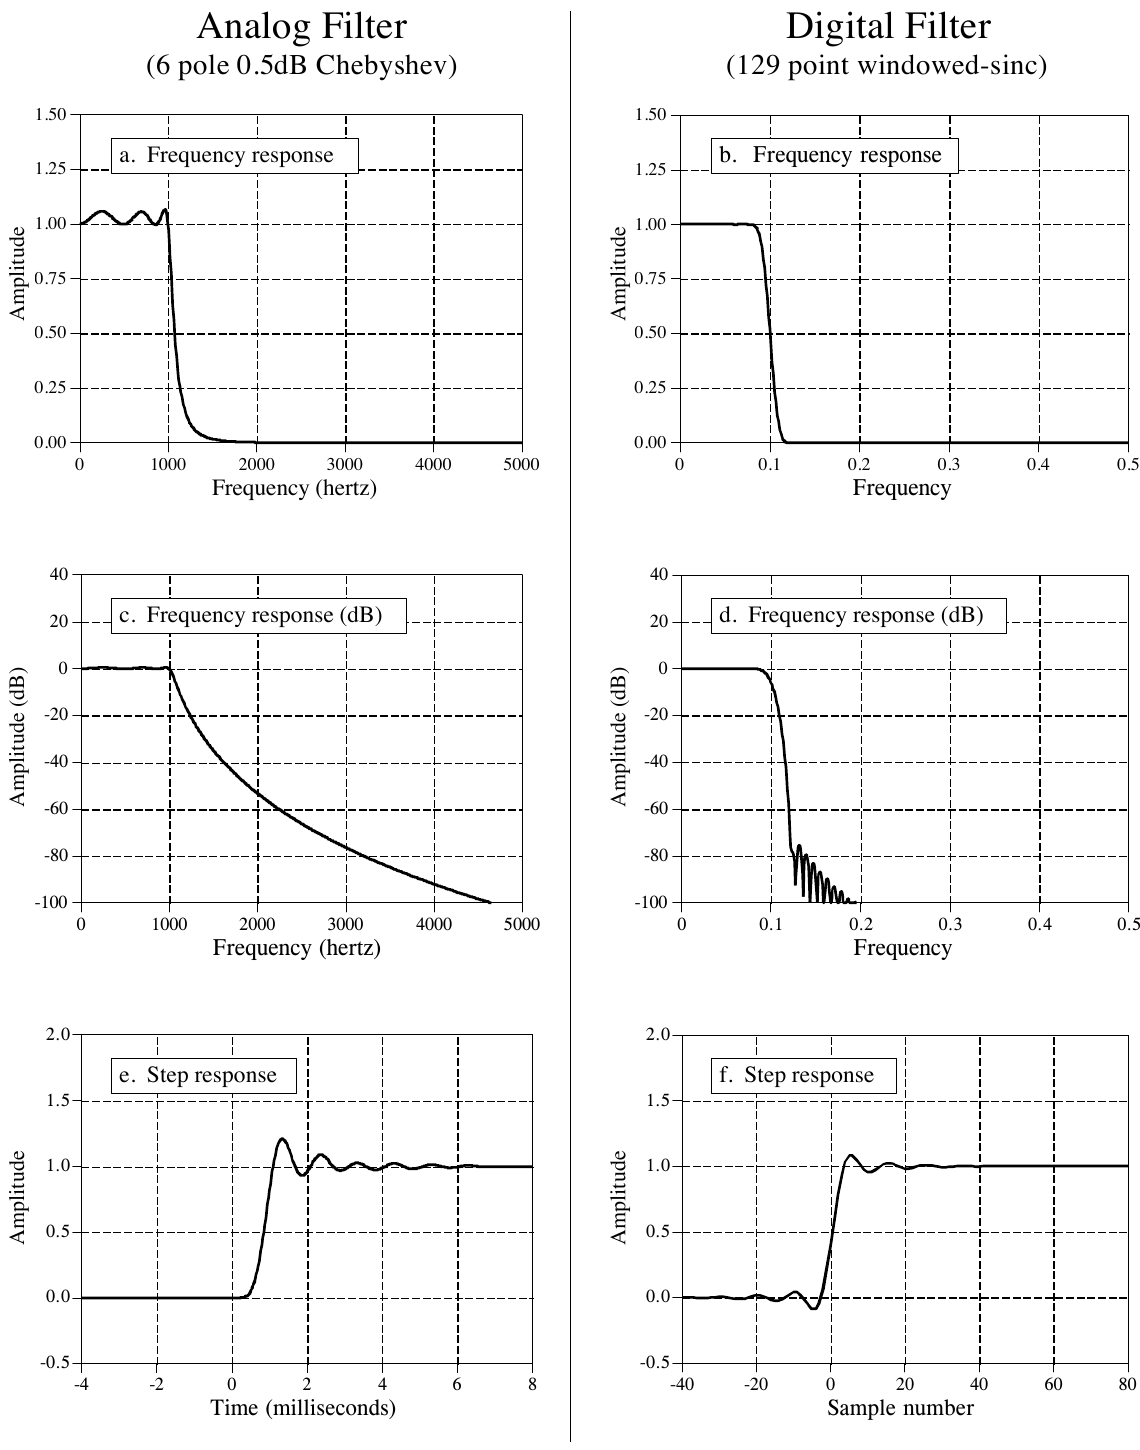
\includegraphics[width=0.950\linewidth,height=0.8\textheight,keepaspectratio]{assets/ch21/fig21-01.png}
\caption*{\textbf{图 21-1　模拟滤波器与数字滤波器的比较。}
数字滤波器在许多方面性能更好，例如：通带纹波，(a) 对
(b)；滚降和阻带衰减，(c) 对 (d)；阶跃响应的对称性，(e) 对
(f)。本例中数字滤波器的截止频率是 10 kHz 采样率的 0.1
倍，这样与模拟滤波器 1 kHz 的截止频率比较才公平。 （左栏 Analog Filter
(6 pole 0.5dB Chebyshev) = 模拟滤波器（六极点、0.5 dB 切比雪夫）；右栏
Digital Filter (129 point windowed-sinc) = 数字滤波器（129 点加窗
sinc）。a、b. Frequency response = 频率响应；c、d.~Frequency response
(dB) = 频率响应（dB）；e、f.~Step response = 阶跃响应。Amplitude =
幅度，Frequency (hertz) = 频率（赫兹），Frequency = 频率，Time
(milliseconds) = 时间（毫秒），Sample number = 采样序号。）}
\end{figure}

接下来看对数刻度下的频率响应，如 (c) 和 (d)
所示。在滚降和阻带衰减(stopband
attenuation)两方面，数字滤波器又一次明显获胜。即使给模拟电路再加几级来提高性能，它仍然没法和数字滤波器相比。例如，假设你需要把这两个参数提高
100 倍。对加窗 sinc
来说，简单改动就能做到；对模拟电路来说，这几乎不可能。数字滤波器再得两分。

两个滤波器的阶跃响应(step response)见 (e) 和
(f)。数字滤波器的阶跃响应在阶跃的下半段和上半段之间是对称的，也就是说它具有线性相位(linear
phase)。模拟滤波器的阶跃响应不对称，也就是说它具有非线性相位(nonlinear
phase)。数字滤波器再得一分。最后，模拟滤波器在阶跃的一侧过冲(overshoot)约
20\%；数字滤波器过冲约
10\%，但阶跃两侧都有。既然两者都不好，这一项不给分。

尽管被打得这么惨，仍然有许多应用应该、甚至必须用模拟滤波器。这和滤波器本身的性能（即输入什么、输出什么）无关，而在于模拟电路相对数字技术的一般优势。第一个优势是速度：数字慢，模拟快。例如，个人计算机用
FFT 卷积，每秒只能处理大约 10,000
个采样。而即使是简单的运算放大器，也能工作在 100 kHz 到 1
MHz，比数字系统快 10 到 100 倍！

模拟相对数字的第二个固有优势是动态范围(dynamic
range)。它有两种。幅度动态范围(amplitude dynamic
range)是系统能通过的最大信号与系统固有噪声之比。例如，一个 12 位 ADC
的饱和电平是 4095，均方根量化噪声是 0.29 个数字量，动态范围约为
14000。相比之下，一个普通运算放大器的饱和电压约 20 伏，内部噪声约 2
微伏，动态范围约为一千万。和前面一样，一个简单的运算放大器就把数字系统打得落花流水。

另一种是频率动态范围(frequency dynamic range)。例如，设计一个能同时处理
0.01 Hz 到 100
kHz（七个十倍程）频率的运放电路很容易。用数字系统去做，计算机就会被数据淹没。比如以
200 kHz 采样，要捕获 0.01 Hz 的一个完整周期需要 2000
万个点。你可能注意到了，数字滤波器的频率响应几乎总是画在线性频率刻度上，而模拟滤波器通常用对数频率显示。这是因为数字滤波器需要线性刻度来展示它们出色的滤波性能，而模拟滤波器需要对数刻度来展示它们巨大的动态范围。

\section{第二场：加窗 sinc vs.~切比雪夫}

加窗 sinc
滤波器和切比雪夫滤波器都是为了把一个频带与另一个频带分开而设计的。加窗
sinc 是用卷积实现的 FIR 滤波器，而切比雪夫是用递归实现的 IIR
滤波器。在频域里，哪个是最好的数字滤波器？我们让它们打一场。

递归滤波器一方的选手是一个纹波
0.5\%、六极点的切比雪夫低通滤波器。要做到公平比较并不简单，因为切比雪夫的频率响应会随截止频率而变。我们用
0.2 的截止频率，并把加窗 sinc 的滤波器核选为 51
点。这样两个滤波器就有相同的 90\% 到 10\% 滚降，如图 21-2(a) 所示。

推推搡搡开始了。递归滤波器的通带有 0.5\% 的纹波，而加窗 sinc
是平坦的。不过，如果需要，我们很容易把递归滤波器的纹波设成
0\%。不给分。图 21-2b 显示加窗 sinc 的阻带衰减比切比雪夫好得多。加窗
sinc 得一分。

\begin{figure}[htbp]
\centering
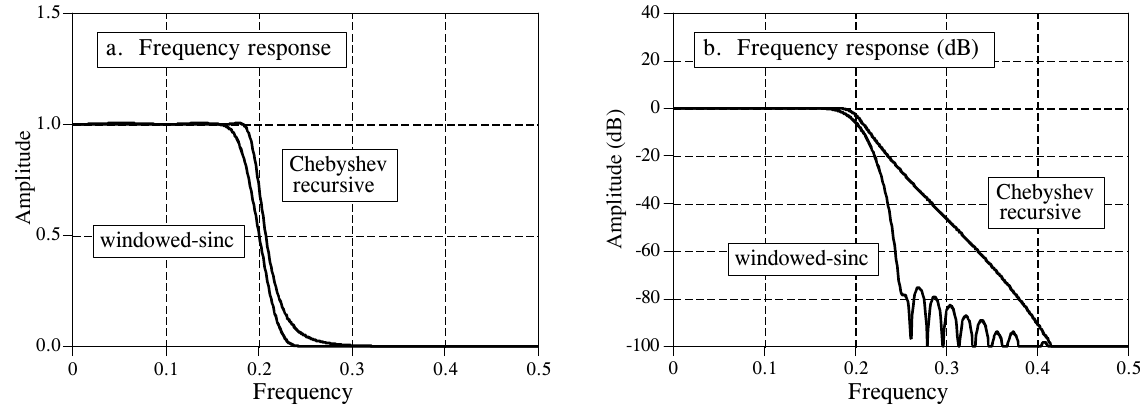
\includegraphics[width=0.950\linewidth,height=0.8\textheight,keepaspectratio]{assets/ch21/fig21-02.png}
\caption*{\textbf{图 21-2　加窗 sinc 与切比雪夫的频率响应。} 图中是 51 点加窗 sinc
滤波器和六极点、0.5\% 纹波切比雪夫递归滤波器的频率响应。加窗 sinc
的阻带衰减更好，但在性能要求中等的应用中两者都能用。两个滤波器的截止频率都是
0.2；对加窗 sinc 是在幅度 0.5 处测量，对递归滤波器是在 0.707 处测量。
（a. Frequency response = 频率响应；b. Frequency response (dB) =
频率响应（dB）。windowed-sinc = 加窗 sinc，Chebyshev recursive =
切比雪夫递归。Amplitude = 幅度，Frequency = 频率。）}
\end{figure}

图 21-3
给出了两个滤波器的阶跃响应。两者都很差，这对频域滤波器来说是意料之中的。递归滤波器是非线性相位，但可以用双向滤波(bidirectional
filtering)来校正。既然两个滤波器在这一项上都这么难看，就算平局。

\begin{figure}[htbp]
\centering
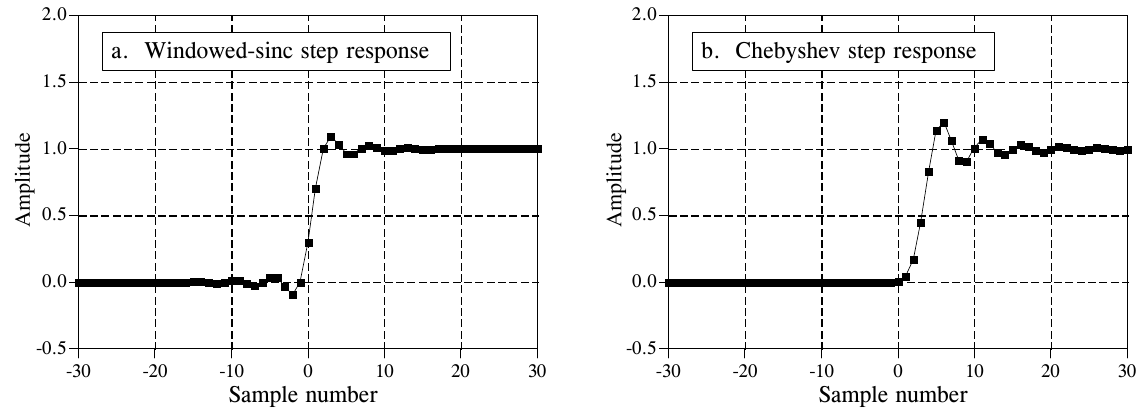
\includegraphics[width=0.950\linewidth,height=0.8\textheight,keepaspectratio]{assets/ch21/fig21-03.png}
\caption*{\textbf{图 21-3　加窗 sinc 与切比雪夫的阶跃响应。} 图中是 51 点加窗 sinc
滤波器和六极点、0.5\%
纹波切比雪夫递归滤波器的阶跃响应，两者的截止频率都是 0.2。加窗 sinc
的阶跃响应略好一些，因为它的过冲更小，而且是零相位(zero phase)。 （a.
Windowed-sinc step response = 加窗 sinc 阶跃响应；b. Chebyshev step
response = 切比雪夫阶跃响应。Amplitude = 幅度，Sample number =
采样序号。原书图注把 Windowed-sinc 印成了 Windowed--sinc。）}
\end{figure}

到目前为止，这两个滤波器差别不大；需要中等性能时，用哪个都行。真正的重拳出在两个关键问题上：最高性能和速度。加窗
sinc
是大力士，而切比雪夫灵活敏捷。假设你遇到一个非常棘手的频率分离问题，比如要从一条
60 赫兹、120 伏的电源线上，分离出骑在上面的一个 61 赫兹、100
毫伏的信号。图 21-4
展示了需要最高性能时这两个滤波器的对比。递归滤波器是纹波 0.5\%
的六极点切比雪夫，这是单精度下截止频率 0.05 时能用的最多极点数。加窗
sinc 使用 1001 点的滤波器核，它由一个 501 点加窗 sinc
滤波器核与自身卷积而成。如第 16 章所示，这样能得到更大的阻带衰减。

\begin{figure}[htbp]
\centering
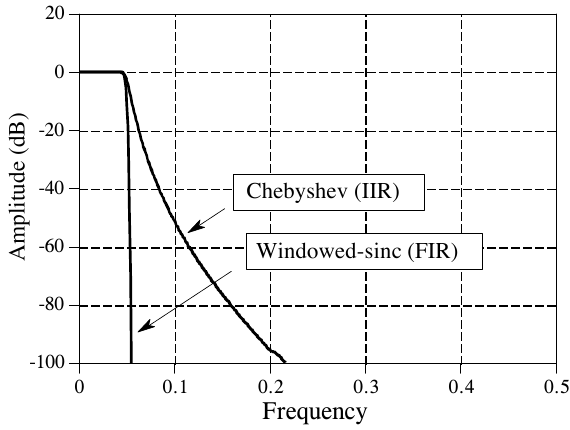
\includegraphics[width=0.475\linewidth,height=0.8\textheight,keepaspectratio]{assets/ch21/fig21-04.png}
\caption*{\textbf{图 21-4　FIR 与 IIR 滤波器的最高性能。} 加窗 sinc
的频率响应几乎可以做成任何需要的形状，而切比雪夫递归滤波器则非常受限。这张图比较了六极点切比雪夫递归滤波器与
1001 点加窗 sinc 滤波器的频率响应。 （Chebyshev (IIR) =
切比雪夫（IIR），Windowed-sinc (FIR) = 加窗 sinc（FIR）。Amplitude (dB)
= 幅度（dB），Frequency =
频率。原书说明排在图的左侧，裁图时已去掉，译文见上。）}
\end{figure}

需要最高性能时，这两个滤波器比起来怎样？加窗 sinc
完胜切比雪夫！即使改进递归滤波器（更多极点、多级实现、双精度等等），它也仍然比不上
FIR 的性能。想到加窗 sinc
才刚刚开始发力，这就更令人印象深刻了。递归滤波器能提供的最高性能有很强的限制；相反，加窗
sinc
可以被推到不可思议的水平。当然，前提是你愿意等结果。这就引出了第二个关键问题：速度。

比较这两个滤波器的速度，就像让法拉利和卡丁车赛跑。图 21-5 显示了加窗
sinc
相比六极点递归滤波器要多花多少执行时间。由于递归滤波器在低频和高频处滚降更快，加窗
sinc
的核必须做得更长才能匹配其性能（也就是为了保持比较的公平）。这就是加窗
sinc 在频率 0 和 0.5 附近执行时间增加的原因。重点是：可以预期 FIR
滤波器比性能相当的 IIR 滤波器慢大约一个数量级（卡丁车：15
英里/小时，法拉利：150 英里/小时）。

\begin{figure}[htbp]
\centering
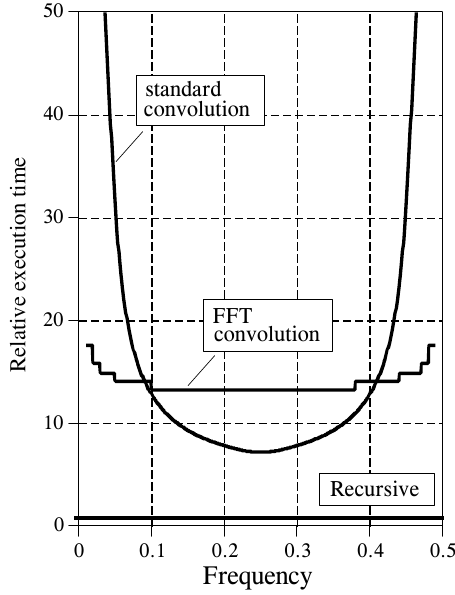
\includegraphics[width=0.379\linewidth,height=0.8\textheight,keepaspectratio]{assets/ch21/fig21-05.png}
\caption*{\textbf{图 21-5　FIR 与 IIR 执行速度的比较。} 这些曲线给出了加窗 sinc
滤波器相对于等效的六极点切比雪夫递归滤波器的执行时间。FIR
滤波器分别用标准卷积和 FFT 卷积两种算法实现，各画了一条曲线。加窗 sinc
的执行时间在低频和高频处上升，因为在这些频率上递归滤波器性能更强，滤波器核必须加长才能跟上。一般来说，IIR
滤波器比性能相当的 FIR 滤波器快一个数量级。 （standard convolution =
标准卷积，FFT convolution = FFT 卷积，Recursive = 递归。Relative
execution time = 相对执行时间，Frequency =
频率。原书说明排在图的左侧，裁图时已去掉，译文见上。）}
\end{figure}

\section{第三场：移动平均 vs.~单极点}

第三场比赛是时域滤波器之战。第一位选手是一个 9
点移动平均滤波器。今天它的对手是一个使用双向技术的单极点递归滤波器。为了得到可比的频率响应，单极点滤波器使用的逐采样衰减系数为
\(x = 0.70\)。战斗从图 21-6
开始，图中给出了两个滤波器各自的频率响应。两者都不怎么样，不过当然，频率分离本来就不是这些滤波器的用途。双方都不得分。

\begin{figure}[htbp]
\centering
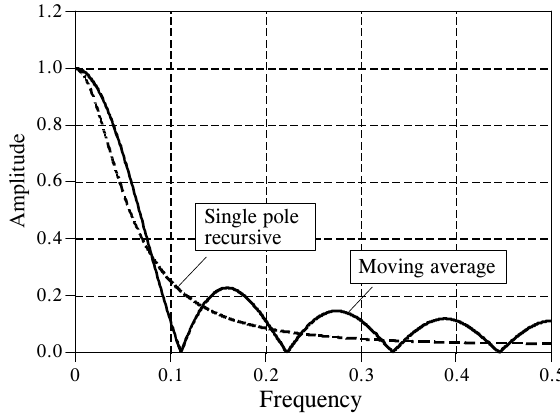
\includegraphics[width=0.467\linewidth,height=0.8\textheight,keepaspectratio]{assets/ch21/fig21-06.png}
\caption*{\textbf{图 21-6　移动平均与单极点滤波器的频率响应。}
这两个滤波器的频率响应都很差，这对时域滤波器来说是意料之中的。 （Single
pole recursive = 单极点递归（虚线），Moving average =
移动平均（实线）。Amplitude = 幅度，Frequency =
频率。原书说明排在图的左侧，裁图时已去掉，译文见上。）}
\end{figure}

图 21-7 给出了两个滤波器的阶跃响应。在 (a)
中，移动平均的阶跃响应是一条直线，这是从一个电平变到另一个电平最快的方式。在
(b) 中，递归滤波器的阶跃响应更平滑，在某些应用中可能更好。双方各得一分。

\begin{figure}[htbp]
\centering
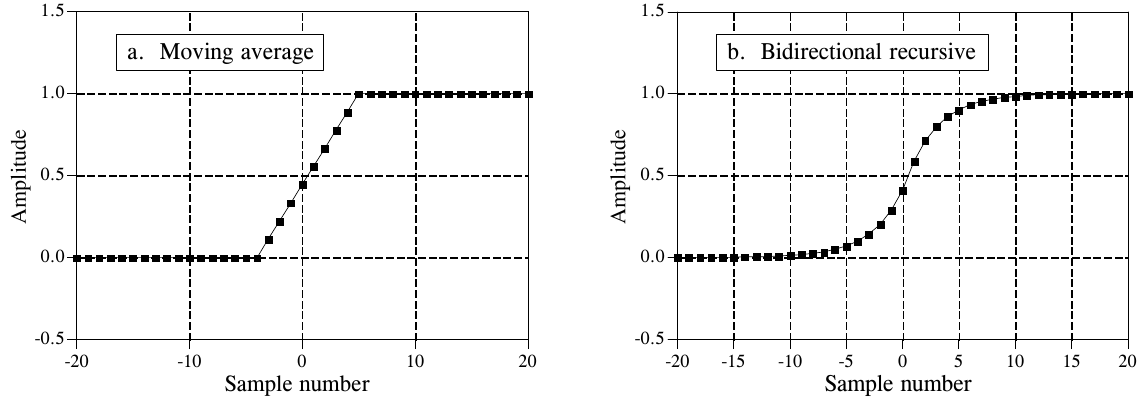
\includegraphics[width=0.950\linewidth,height=0.8\textheight,keepaspectratio]{assets/ch21/fig21-07.png}
\caption*{\textbf{图 21-7　移动平均与双向单极点滤波器的阶跃响应。}
移动平均的阶跃响应在更少的采样内完成，而单极点滤波器的阶跃响应更平滑。
（a. Moving average = 移动平均；b. Bidirectional recursive =
双向递归。Amplitude = 幅度，Sample number = 采样序号。）}
\end{figure}

这两个滤波器在性能上势均力敌，两者之间的选择往往取决于个人偏好。不过，有两种情况下其中一个略占上风。它们取决于开发时间与执行时间之间的权衡。第一种情况，你想缩短开发时间，愿意接受较慢的滤波器。例如，你可能只是一次性地需要过滤几千个点。整个程序几秒钟就跑完，花时间优化算法毫无意义。几乎肯定会用浮点数。可选的是用卷积实现的移动平均滤波器，或者单极点递归滤波器。这里的赢家是递归滤波器：它编写和修改起来稍微容易一点，而且执行快得多。

第二种情况正好相反：你的滤波器必须尽可能快，你也愿意多花开发时间来做到这一点。例如，这个滤波器可能是某个商业产品的一部分，可能要运行几百万次。为了获得最高速度，你可能会用整数。可选的滤波器是用递归实现的移动平均滤波器，或者用查找表(look-up
table)或整数运算实现的单极点递归滤波器。赢家是移动平均滤波器：它执行更快，也不会受到整数运算在开发和执行上的那些问题影响。

% !TEX root = ../main.tex
% 本文件由 build-tex.sh 从 22-DSP指南-第22章中译.md 生成，改内容请改 md 后重新生成

\chapter{音频处理}\label{ch-22}

音频处理(audio
processing)涵盖许多不同的领域，它们都与把声音呈现给人类听众有关。其中有三个领域最为突出：(1)
高保真音乐重放，比如音频 CD；(2)
语音通信，也就是电话网络的另一种说法；(3)
合成语音，即由计算机生成和识别人的语音。这些应用的目标和难题各不相同，但它们由同一位裁判联系在一起：人耳。数字信号处理已经给这些以及音频处理的其他领域带来了革命性的变化。

\section{人的听觉}

人耳是一个极其复杂的器官。更麻烦的是，来自两只耳朵的信息还要在一个令人费解的神经网络------人脑------中合并。请记住，下面只是一个简短的概述；与人的听觉相关的微妙效应和尚未弄清的现象还有很多。

图 22-1 画出了构成人耳的主要结构和过程。外耳(outer
ear)由两部分组成：一是长在头侧、看得见的皮肤和软骨组成的耳廓，二是耳道(ear
canal)，一根直径约 0.5 cm、向头内延伸约 3 cm
的管子。这些结构把环境中的声音引向位于颅骨内部、受到安全保护的敏感的中耳和内耳器官。耳道末端绷着一层薄薄的组织，叫鼓膜(tympanic
membrane，ear drum)。声波打在鼓膜上，使它振动。中耳(middle
ear)是一组小骨头，把这种振动传到耳蜗(cochlea，即内耳)，在那里转换成神经冲动。耳蜗是一根充满液体的管子，直径约
2 mm，长约 3 cm。虽然图 22-1
把它画成直的，但耳蜗其实是盘卷起来的，看上去像个小蜗牛壳。事实上，cochlea
一词就来自希腊语的''蜗牛''。

\begin{figure}[htbp]
\centering
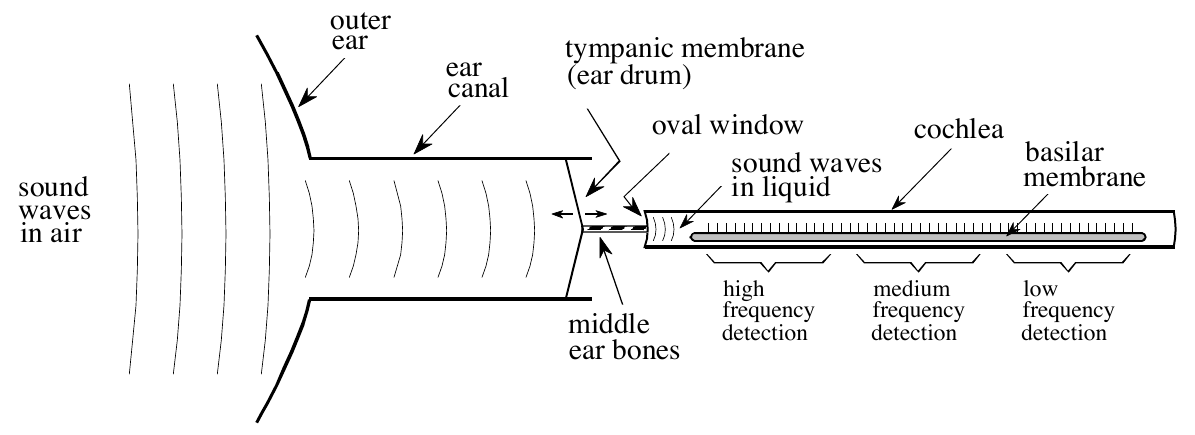
\includegraphics[width=0.996\linewidth,height=0.8\textheight,keepaspectratio]{assets/ch22/fig22-01.png}
\caption*{\textbf{图 22-1　人耳的功能示意图。}
外耳收集环境中的声波，把它们导向鼓膜。鼓膜是一层薄薄的组织，随空气中的波形同步振动。中耳的听小骨（锤骨、砧骨和镫骨）把这些振动传到卵圆窗------充满液体的耳蜗上的一层柔软的膜。耳蜗里有基底膜，它支撑着约
12,000
个构成耳蜗神经的神经细胞。由于基底膜各处的硬度不同，每个神经细胞只对很窄的一段音频频率有反应，这使耳朵成了一台频谱分析仪。
（sound waves in air = 空气中的声波，outer ear = 外耳，ear canal =
耳道，tympanic membrane (ear drum) = 鼓膜，middle ear bones =
听小骨，oval window = 卵圆窗，sound waves in liquid =
液体中的声波，cochlea = 耳蜗，basilar membrane = 基底膜，high / medium /
low frequency detection = 高 / 中 / 低频检测。原书图注把 responds 误写成
responses。）}
\end{figure}

声波试图从空气进入液体时，只有一小部分声音能穿过分界面，其余能量都被反射回去。这是因为空气的机械阻抗(mechanical
impedance)低（密度低、可压缩性高，所以声压低、质点速度高），而液体的机械阻抗高。用不那么专业的话说，在水里挥手比在空气里挥手费劲。机械阻抗的这种差异，使得大部分声音在空气/液体界面上被反射。

中耳是一个阻抗匹配网络，用来提高进入内耳液体的声能比例。比如鱼就没有鼓膜和中耳，因为它们不需要在空气中听声音。阻抗转换主要来自鼓膜（从空气接收声音）与卵圆窗(oval
window，把声音传入液体，见图 22-1)的面积差。鼓膜面积约 60
mm²，而卵圆窗面积约 4
mm²。由于压强等于力除以面积，这个面积差使声波的压强提高约 15 倍。

耳蜗里有基底膜(basilar membrane)，它是约 12,000
个感觉细胞的支撑结构，这些细胞构成耳蜗神经。基底膜在靠近卵圆窗处最硬，越往另一端越柔软，因此能起到频谱分析仪的作用。遇到高频信号时，基底膜在较硬的地方共振，于是靠近卵圆窗的神经细胞被激发。同样，低频声音激发基底膜远端的神经细胞。这使得耳蜗神经中特定的纤维只对特定的频率起反应。这种组织方式叫位置原理(place
principle)，并且沿着整条听觉通路一直保持到大脑。

人的听觉还使用另一种信息编码方式，叫齐射原理(volley
principle)。神经细胞通过产生叫动作电位(action
potential)的短暂电脉冲来传递信息。基底膜上的神经细胞可以对振动的每个周期各产生一个动作电位，以此对音频信息编码。例如，一个
200 Hz 的声波可以用一个每秒产生 200
个动作电位的神经元来表示。不过这只在大约 500 Hz
以下的频率有效，这是神经元产生动作电位的最高速率。人耳克服这个问题的办法是让几个神经细胞轮流完成这项任务。例如，一个
3000 Hz 的音调可以用十个神经细胞轮流以每秒 300
次的速度发放来表示。这样齐射原理的适用范围就扩展到约 4
kHz，再往上就只用位置原理了。

表 22-1 给出了声强与感知响度之间的关系。声强通常用对数刻度表示，叫分贝
SPL(decibel SPL，Sound Power Level)。在这个刻度上，0 dB SPL
对应的声波功率是 \(10^{-16}\)
W/cm²，大约是人耳能察觉的最弱的声音。正常说话约 60 dB SPL，而到约 140 dB
SPL 时耳朵会感到疼痛并受到损伤。

\begin{quote}
\textbf{译注：} SPL 通常是 Sound Pressure
Level（声压级）的缩写，原书写成 Sound Power
Level（声功率级）。本章按原书用的是功率（W/cm²），两种叫法在这里的分贝数相同，不影响理解。
\end{quote}

\textbf{表 22-1　声强的单位。} 声强用单位面积上的功率（比如
W/cm²）表示，更常用的是叫分贝 SPL 的对数刻度。如表所示，人的听觉在 1 kHz
到 4 kHz 之间最灵敏。（表中自上而下声音越来越轻。）

{\def\LTcaptype{none} % do not increment counter
\begin{longtable}[]{@{}
  >{\raggedright\arraybackslash}p{(\linewidth - 4\tabcolsep) * \real{0.3333}}
  >{\raggedright\arraybackslash}p{(\linewidth - 4\tabcolsep) * \real{0.3333}}
  >{\raggedright\arraybackslash}p{(\linewidth - 4\tabcolsep) * \real{0.3333}}@{}}
\toprule\noalign{}
\begin{minipage}[b]{\linewidth}\raggedright
W/cm²
\end{minipage} & \begin{minipage}[b]{\linewidth}\raggedright
分贝 SPL
\end{minipage} & \begin{minipage}[b]{\linewidth}\raggedright
声音举例
\end{minipage} \\
\midrule\noalign{}
\endhead
\bottomrule\noalign{}
\endlastfoot
\(10^{-2}\) & 140 dB & 疼痛 \\
\(10^{-3}\) & 130 dB & \\
\(10^{-4}\) & 120 dB & 不适 \\
\(10^{-5}\) & 110 dB & 手提凿岩机、摇滚音乐会 \\
\(10^{-6}\) & 100 dB & \\
\(10^{-7}\) & 90 dB &
OSHA（美国职业安全与健康管理局）规定的工业噪声上限 \\
\(10^{-8}\) & 80 dB & \\
\(10^{-9}\) & 70 dB & \\
\(10^{-10}\) & 60 dB & 正常谈话 \\
\(10^{-11}\) & 50 dB & \\
\(10^{-12}\) & 40 dB & 100 Hz 处能听到的最弱声音 \\
\(10^{-13}\) & 30 dB & \\
\(10^{-14}\) & 20 dB & 10 kHz 处能听到的最弱声音 \\
\(10^{-15}\) & 10 dB & \\
\(10^{-16}\) & 0 dB & 3 kHz 处能听到的最弱声音 \\
\(10^{-17}\) & −10 dB & \\
\(10^{-18}\) & −20 dB & \\
\end{longtable}
}

人能听到的最响和最轻的声音之间相差约 120
dB，幅度上相差一百万倍。信号变化约 1 dB（幅度变化
12\%）时，听者就能察觉到响度的变化。换句话说，从最轻的耳语到最响的雷声，人能分辨的响度等级只有大约
120
级。耳朵的灵敏度惊人：听很微弱的声音时，鼓膜振动的幅度比单个分子的直径还小！

响度的感知大致与声功率的 1/3
次方成正比。例如，如果把声功率提高到十倍，听者会说响度大约增加到两倍（\(10^{1/3} \approx 2\)）。这给消除讨厌的环境声音带来了大麻烦，比如隔壁公寓那套加大功率的音响。假设你辛辛苦苦用完美的隔音材料把墙面盖住了
99\%，只因为门、墙角、通风口等漏掉了 1\% 的面积。尽管声功率已降到原来的
1\%，感知到的响度却只降到约 \(0.01^{1/3} \approx 0.2\)，也就是 20\%。

人的听觉范围一般认为是 20 Hz 到 20 kHz，但对 1 kHz 到 4 kHz
之间的声音要灵敏得多。例如，听者在 3 kHz 能察觉低到 0 dB SPL 的声音，在
100 Hz 却需要 40 dB SPL（幅度要大 100 倍）。在 3 kHz
处，两个音调的频率相差超过约 0.3\%，听者就能分辨出它们不同；在 100 Hz
处这个数字增大到 3\%。作为对比，钢琴上相邻两个键的频率相差约 6\%。

两只耳朵的主要好处是能辨别声音的方向。人能分辨相隔仅三度的两个声源，大约相当于
10 米外一个人的宽度。方向信息通过两种不同的途径获得。第一，约 1 kHz
以上的频率会被头部明显遮挡。也就是说，离声源近的那只耳朵收到的信号比头另一侧的耳朵强。第二条方向线索是：远离声源的那只耳朵因为距离更远，听到声音会比近的那只稍晚一些。按典型的头部尺寸（约
22 cm）和声速（约 340 m/s）计算，三度的角度分辨需要约 30
微秒的计时精度。由于这种计时要依赖齐射原理，这条方向线索主要用于约 1 kHz
以下的声音。

转动头部、观察信号的变化，对这两种方向信息都大有帮助。当两只耳朵听到完全相同的声音时，比如用耳机听单声道声音，会出现一种有趣的感觉：大脑会认定声音来自听者的脑袋正中！

人的听觉虽然能判断声音来自哪个方向，却很难判断声源有多远。这是因为声波中能提供距离信息的线索很少。人的听觉会隐约觉得高频声音近、低频声音远，这是因为声波在长距离传播中会损失较高的频率。回声成分是另一条微弱的距离线索，它让人感知房间的大小。例如，大礼堂中的声音会带有间隔约
100 毫秒的回声，而小办公室里典型的间隔是 10
毫秒。有些物种用主动声呐(active
sonar)解决了测距问题。例如，蝙蝠和海豚发出咔哒声和尖叫声，这些声音从附近的物体反射回来。通过测量发出声音和收到回声之间的间隔，这些动物能以约
1 cm
的分辨率定位物体。实验表明，有些人，尤其是盲人，也能在一定程度上利用主动回声定位。

\section{音色}

对一个持续的声音（比如乐器奏出的一个音符）的感知，通常分为三部分：响度(loudness)、音高(pitch)和音色(timbre，读作
``timber'')。响度是声波强度的度量，前面已经讲过。音高是声音中基频成分的频率，也就是波形重复的频率。这两种感知虽然都有一些微妙之处，但都能直接对应到容易刻画的物理量上。

音色要复杂一些，它由信号的谐波(harmonic)成分决定。图 22-2
画了两个波形，每个都由一个幅度为 1 的 1 kHz 正弦波加上一个幅度为 1/2 的
3 kHz 正弦波构成。两者的区别在于，(b)
中的那个在相加之前把较高的频率反相了。换句话说，三次谐波（3
kHz）相对于一次谐波（1 kHz）相移了 180
度。尽管时域波形大不相同，这两个信号听起来却一模一样。这是因为听觉依据的是各频率的幅度，而对它们的相位非常不敏感。时域波形的形状只与听觉间接相关，在音频系统中通常不予考虑。

\begin{figure}[htbp]
\centering
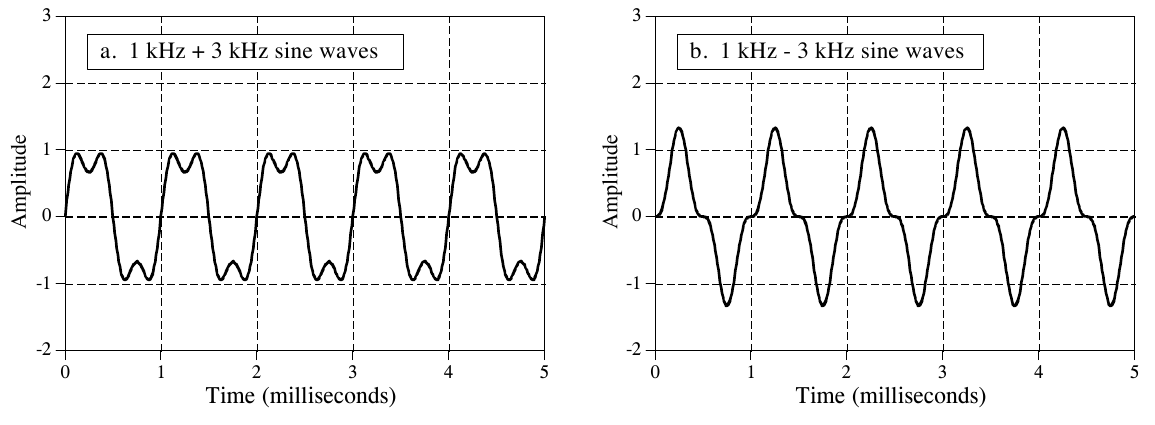
\includegraphics[width=0.963\linewidth,height=0.8\textheight,keepaspectratio]{assets/ch22/fig22-02.png}
\caption*{\textbf{图 22-2　人耳对相位的感知。}
人耳对各正弦分量之间的相对相位非常不敏感。例如，这两个波形听起来一模一样，因为它们各分量的幅度相同，尽管相对相位不同。
（a. 1 kHz + 3 kHz sine waves = 1 kHz 与 3 kHz 正弦波相加；b. 1 kHz − 3
kHz sine waves = 1 kHz 与 3 kHz 正弦波相减。Amplitude = 幅度，Time
(milliseconds) = 时间（毫秒）。）}
\end{figure}

考察声音在环境中怎样传播，就能理解耳朵为什么对相位不敏感。假设你在一个小房间里听对面的人说话。到达你耳朵的声音，很大一部分是从墙壁、天花板和地板反射来的。由于声音的传播与频率有关（比如衰减、反射和共振），不同频率会经由不同的路径到达你的耳朵。这意味着你在房间里走动时，各频率的相对相位会发生变化。由于耳朵忽略这些相位变化，你在移动时会觉得说话声没有变。从物理的角度看，音频信号在复杂环境中传播时，其相位会变得随机。换句话说，耳朵对相位不敏感，是因为相位几乎不含有用的信息。

不过，也不能说耳朵对相位完全充耳不闻。这是因为相位的改变可能会重新安排音频信号的时间顺序。一个例子是啁啾系统(chirp
system，第 11
章)，它把一个冲激变成一个持续时间长得多的信号。这两个声音虽然只在相位上不同，耳朵却能区分它们，因为它们的持续时间不同。这在很大程度上只是个奇特现象，在正常的听音环境中不会发生。

假设我们请一位小提琴手拉一个音，比如中央 C 下面的
A。在示波器上显示这个波形，它看起来很像图 22-3a
中的锯齿波(sawtooth)。这是小提琴弓毛上涂的黏性松香造成的。弓在弦上拉过时，弦先粘在弓上、被拉过去，最后挣脱开来，波形就这样形成了。这个循环一再重复，就得到了锯齿波形。

\begin{figure}[htbp]
\centering
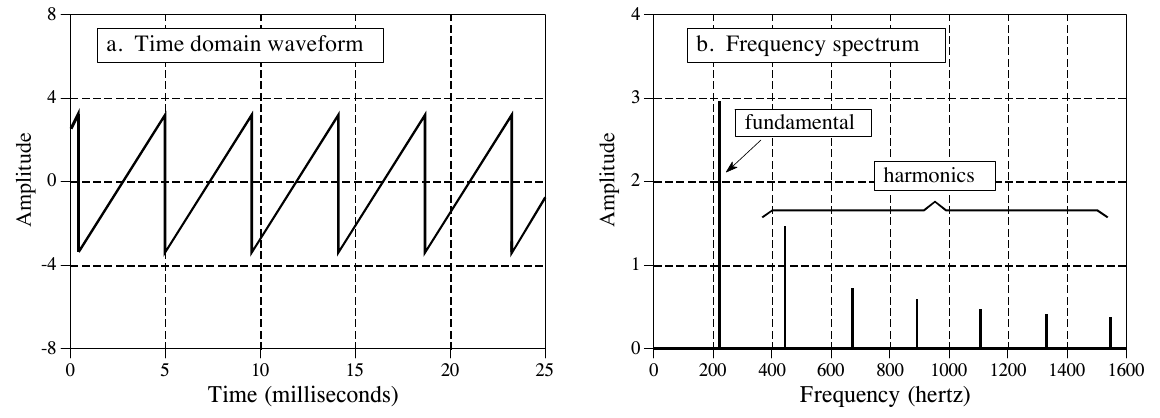
\includegraphics[width=0.967\linewidth,height=0.8\textheight,keepaspectratio]{assets/ch22/fig22-03.png}
\caption*{\textbf{图 22-3　小提琴的波形。} 拉奏的小提琴产生锯齿波，如 (a)
所示。耳朵听到的声音如 (b) 所示：基频加上各次谐波。 （a. Time domain
waveform = 时域波形；b. Frequency spectrum = 频谱，fundamental =
基频，harmonics = 谐波。Amplitude = 幅度，Time (milliseconds) =
时间（毫秒），Frequency (hertz) = 频率（赫兹）。）}
\end{figure}

图 22-3b 显示了耳朵怎样感知这个声音：220 Hz 的频率，加上 440、660、880
Hz
等处的谐波。如果在另一件乐器上奏出这个音，波形看起来会不同，但耳朵听到的仍然是
220 Hz
加上各次谐波。由于两件乐器奏这个音时产生相同的基频，它们听起来相似，称为音高相同。由于谐波的相对幅度不同，它们听起来又不会完全一样，称为音色不同。

人们常说音色由波形的形状决定。这话没错，但有点误导。音色的感知来自耳朵对谐波的检测。虽然谐波成分由波形的形状决定，但由于耳朵对相位不敏感，这种关系非常单向。也就是说，一个特定的波形只有一种音色，而一种特定的音色却对应无穷多种可能的波形。

耳朵非常习惯听''基频加谐波''。如果给听者放 1 kHz 和 3 kHz
两个正弦波的组合，他们会说听起来自然悦耳。如果换成 1 kHz 和 3.1 kHz
的正弦波，就会很难听。

这就是标准音阶的基础，如图 22-4
中的钢琴键盘所示。敲击钢琴最左边的键，产生 27.5 Hz 的基频，外加
55、110、220、440、880 Hz
等处的谐波（这些频率之间也有谐波，但对这里的讨论不重要）。这些谐波对应键盘上其他键产生的基频。具体来说，每隔七个白键，就是最左边那个键的一个谐波。也就是说，从左数第八个键的基频是
55 Hz，第 15 个键的基频是 110
Hz，依此类推。由于彼此互为谐波，这些键弹起来听着相似，一起弹时也很和谐。因此它们都叫做音符
A。同样，每个 A 右边紧挨着的白键叫
B，它们也都互为谐波。这个规律对七个音符 A、B、C、D、E、F、G 重复。

\begin{figure}[htbp]
\centering
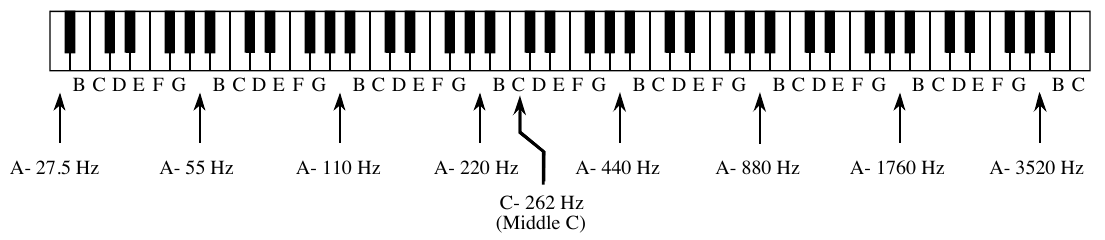
\includegraphics[width=0.921\linewidth,height=0.8\textheight,keepaspectratio]{assets/ch22/fig22-04.png}
\caption*{\textbf{图 22-4　钢琴键盘。}
钢琴键盘是一个对数频率刻度，每隔七个白键基频翻一倍。这些白键依次是音符
A、B、C、D、E、F 和 G。 （A- 27.5 Hz 等 = 各个 A 键的基频；C- 262 Hz
(Middle C) = 中央 C，262 Hz。）}
\end{figure}

八度(octave)这个术语指频率相差两倍。在钢琴上，一个八度包含八个白键，这就是名字的由来（octo
在拉丁语中是''八''）。换句话说，钢琴每隔七个白键频率翻一倍，整个键盘跨越七个多八度。人的听觉范围一般说是
20 Hz 到 20
kHz，大约相当于钢琴键盘左边再延伸半个八度、右边再延伸两个八度。由于八度是按每隔固定键数频率翻倍来定的，它是频率的一种对数表示。这一点很重要，因为音频信息一般也是这样分布的。例如，50
Hz 到 100 Hz 这一个八度所携带的音频信息，与 10 kHz 到 20 kHz
这一个八度一样多。尽管钢琴只覆盖人能听到的频率的约 20\%（20 kHz 中的 4
kHz），它却能产生人能感知的音频信息的 70\% 以上（10 个八度中的 7
个）。同样，在成年人的一生中，能听到的最高频率会从约 20 kHz 降到 10
kHz。但这只损失了约 10\%
的听力（十个八度中的一个）。下面会看到，信息的这种对数分布直接影响音频信号所需的采样率。

\section{音质与数据率}

设计数字音频系统时，要问两个问题：(1) 它需要听起来多好？(2)
能容忍多高的数据率？对这两个问题的回答通常落入三类中的一类。第一，高保真音乐，音质最重要，几乎任何数据率都能接受。第二，电话通信，要求语音听起来自然，同时数据率要低以降低系统成本。第三，压缩语音，降低数据率非常重要，音质上的一些不自然可以容忍。这包括军用通信、手机，以及用于语音信箱和多媒体的数字存储语音。

表 22-2
给出了这三类的音质与数据率之间的权衡。高保真音乐系统采样得足够快（44.1
kHz）、精度足够高（16
位），几乎能捕捉人能听到的所有声音。这种极好的音质是以高数据率为代价的：44.1
kHz × 16 位 = 706k 位/秒。这纯粹是蛮力。

音乐需要 20 kHz 的带宽，而听起来自然的语音只需要约 3.2
kHz。尽管频率范围降到了只有 16\%（20 kHz 中的 3.2
kHz），信号仍包含原来声音信息的 80\%（10 个八度中的 8
个）。电信系统通常以约 8 kHz
的采样率工作，语音听起来自然，但音乐质量大打折扣。你大概已经熟悉这种音质差别：FM
电台以将近 20 kHz 的带宽广播，而 AM 电台限制在约 3.2 kHz。在 AM
电台上人声听起来正常，音乐却单薄乏味。

只传语音的系统还把每个采样的精度从 16 位降到 12
位，音质几乎没有可察觉的变化。如果把量化步长做成不均匀的，还能降到每个采样只用
8 位。这是一种广泛使用的方法，叫压扩(companding)，本章后面会讲。8 kHz
的采样率配上每采样 8 位的 ADC 精度，得到 64k
位/秒的数据率。这是自然语音的''蛮力''数据率。注意语音所需的数据率还不到高保真音乐的
10\%。

\textbf{表 22-2　音频数据率与音质。}
数字化音频信号的音质取决于它的数据率，即采样率与每采样位数的乘积。可以分为三类：高保真音乐（706
k 位/秒）、电话质量语音（64 k 位/秒）和压缩语音（4 k 位/秒）。

\begingroup\footnotesize\setlength{\tabcolsep}{3pt}

{\def\LTcaptype{none} % do not increment counter
\begin{longtable}[]{@{}
  >{\raggedright\arraybackslash}p{(\linewidth - 10\tabcolsep) * \real{0.1667}}
  >{\raggedright\arraybackslash}p{(\linewidth - 10\tabcolsep) * \real{0.1667}}
  >{\raggedright\arraybackslash}p{(\linewidth - 10\tabcolsep) * \real{0.1667}}
  >{\raggedright\arraybackslash}p{(\linewidth - 10\tabcolsep) * \real{0.1667}}
  >{\raggedright\arraybackslash}p{(\linewidth - 10\tabcolsep) * \real{0.1667}}
  >{\raggedright\arraybackslash}p{(\linewidth - 10\tabcolsep) * \real{0.1667}}@{}}
\toprule\noalign{}
\begin{minipage}[b]{\linewidth}\raggedright
所需音质
\end{minipage} & \begin{minipage}[b]{\linewidth}\raggedright
带宽
\end{minipage} & \begin{minipage}[b]{\linewidth}\raggedright
采样率
\end{minipage} & \begin{minipage}[b]{\linewidth}\raggedright
位数
\end{minipage} & \begin{minipage}[b]{\linewidth}\raggedright
数据率（位/秒）
\end{minipage} & \begin{minipage}[b]{\linewidth}\raggedright
说明
\end{minipage} \\
\midrule\noalign{}
\endhead
\bottomrule\noalign{}
\endlastfoot
高保真音乐（CD） & 5 Hz～20 kHz & 44.1 kHz & 16 位 & 706k &
连最挑剔的发烧友也满意。比人的听觉还好。 \\
电话质量语音 & 200 Hz～3.2 kHz & 8 kHz & 12 位 & 96k &
语音质量好，但放音乐很差。 \\
（采用压扩） & 200 Hz～3.2 kHz & 8 kHz & 8 位 & 64k & 非线性 ADC
把数据率降低 50\%。非常常用的技术。 \\
线性预测编码的语音 & 200 Hz～3.2 kHz & 8 kHz & 12 位 & 4k & DSP
语音压缩技术。数据率很低，语音质量差。 \\
\end{longtable}
}

\endgroup

64k
位/秒的数据率代表把采样和量化理论直接用于音频信号的结果。进一步降低数据率的技术，都基于去除语音信号中固有的冗余来压缩数据流。数据压缩是第
27 章的主题。压缩音频信号最有效的方法之一是线性预测编码(Linear
Predictive Coding，LPC)，它有好几种变体和分支。根据所需的语音质量，LPC
能把数据率降到只有 2～6k 位/秒。本章后面讲语音合成时还会回到 LPC。

\section{高保真音频}

发烧友(audiophile)追求极致的音质，其他一切因素都是次要的。如果要用一个词来形容这种心态，那就是：过度(overkill)。这些系统不只是匹配人耳的能力，而是要超越听觉的极限。只有这样才能确保重放的音乐完美无瑕。数字音频是随激光唱片(compact
laser disc，即 CD)来到世间的。这是一场音乐的革命：CD
系统的音质远远超过唱片、磁带等老系统。DSP 一直站在这项技术的最前沿。

图 22-5
画出了激光唱片的表面，就像用高倍显微镜看到的那样。主表面是光亮的（能反光），数字信息存储为一串用激光烧在表面上的暗色凹坑(pit)。信息排成一条单独的轨道，从外向内螺旋，和黑胶唱片一样。从螺旋的外圈向内圈读取信息时，CD
的转速从约 210 rpm 变到 480 rpm，使扫描线速度保持恒定的 1.2
米/秒。（相比之下，黑胶唱片以固定转速旋转，比如 33、45 或 78
rpm。）播放时，一个光学传感器检测表面是反光还是不反光，生成相应的二进制信息。

\begin{figure}[htbp]
\centering
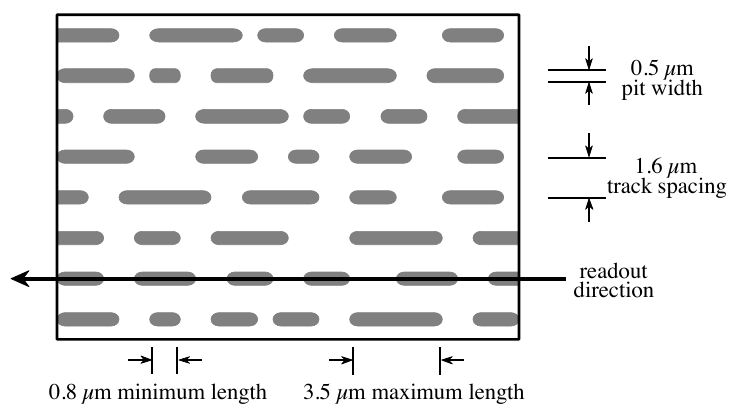
\includegraphics[width=0.617\linewidth,height=0.8\textheight,keepaspectratio]{assets/ch22/fig22-05.png}
\caption*{\textbf{图 22-5　CD 的表面。} 在 CD 表面烧出微米大小的凹坑来表示 1 和
0。由此得到的数据密度是每平方微米 1 位，即每平方毫米一百万位。凹坑深
0.16 µm。 （pit width = 凹坑宽度 0.5 µm，track spacing = 轨道间距 1.6
µm，readout direction = 读出方向，minimum length = 最短长度 0.8
µm，maximum length = 最长长度 3.5
µm。原书图注排在图左侧，裁图时已去掉，译文见上。）}
\end{figure}

按图 22-5 的几何尺寸，CD 每平方微米存储约 1
位，相当于每平方毫米一百万位，整张盘 150
亿位。这和集成电路制造所用的特征尺寸差不多，而且是有原因的。光的一个特性是：它不能被聚焦到小于约半个波长，即
0.3 µm。由于集成电路和激光唱片都是用光学手段制造的，光在 0.3 µm
以下的模糊限制了能用多小的特征尺寸。

图 22-6 是一个典型 CD 播放系统的框图。原始数据率是每秒 430
万位，相当于每 0.28 µm 轨道长度 1 位。然而，这与 CD
规定的几何尺寸冲突：每个凹坑不能短于 0.8 µm，也不能长于 3.5
µm。换句话说，每个二进制 1 都必须是一组 3 到 13 个 1
中的一部分。这样做的好处是降低光学读取头造成的误码率，但怎样迫使二进制数据服从这种奇怪的成组规则呢？

答案是一种叫八到十四调制(eight-to-fourteen
modulation，EFM)的编码方案。不是把一个字节的数据直接存到盘上，而是让这 8
位通过一张查找表，查出 14 位。这 14
位具备所需的成组特性，被存储到激光唱片上。播放时，从盘上读出的二进制值通过
EFM 查找表的逆表，每组 14 位又变回正确的 8 位。

\begin{figure}[htbp]
\centering
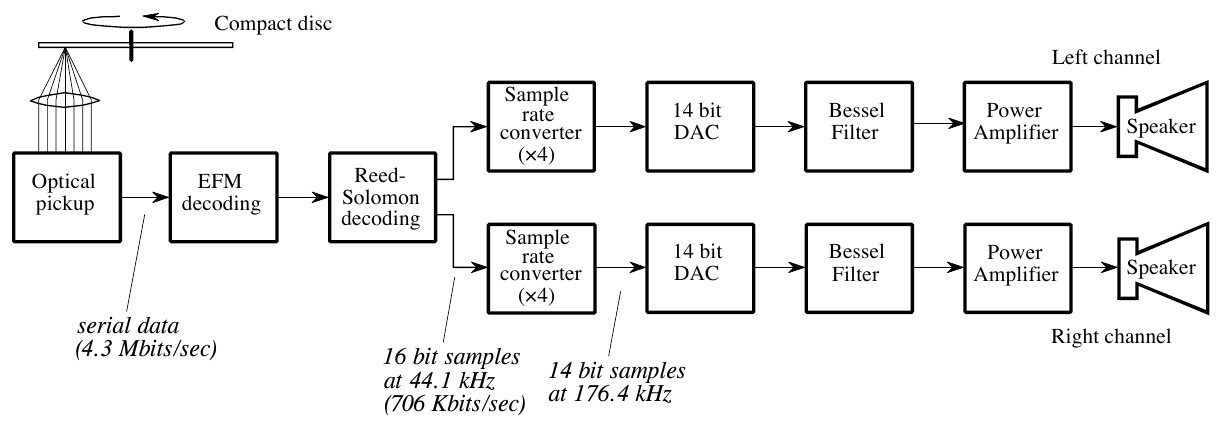
\includegraphics[width=1.000\linewidth,height=0.8\textheight,keepaspectratio]{assets/ch22/fig22-06.png}
\caption*{\textbf{图 22-6　CD 播放系统框图。} 用光学传感器从盘上取出数字信息，经过
EFM 解码和里德-所罗门(Reed-Solomon)解码校正，再转换成立体声模拟信号。
（Compact disc = 激光唱片，Optical pickup = 光学读取头，EFM decoding =
EFM 解码，Reed-Solomon decoding = 里德-所罗门解码，Sample rate converter
(×4) = 采样率转换器（×4），14 bit DAC = 14 位 DAC，Bessel Filter =
贝塞尔滤波器，Power Amplifier = 功率放大器，Speaker = 扬声器，Left /
Right channel = 左 / 右声道；serial data (4.3 Mbits/sec) = 串行数据（4.3
M 位/秒），16 bit samples at 44.1 kHz (706 Kbits/sec) = 44.1 kHz 的 16
位采样（706 k 位/秒），14 bit samples at 176.4 kHz = 176.4 kHz 的 14
位采样。）}
\end{figure}

除了 EFM，数据还以一种叫两级里德-所罗门编码(two-level Reed-Solomon
coding)的格式编码。这需要把左右两个立体声声道与用于检错和纠错的数据组合在一起。播放时检测到的数字错误，或者利用编码方案中的冗余数据纠正，或者通过在相邻采样之间插值来掩盖，或者把采样值设为零来静音。这些编码方案使数据率增加到三倍，即立体声音频信号的
1.4 M 位/秒对盘上存储的 4.3 M 位/秒。

解码和纠错之后，音频信号表示为 44.1 kHz 采样率下的 16
位采样。最简单的系统可以把这些信号送进一个 16 位
DAC，再接一个模拟低通滤波器。然而，这需要高性能的模拟电子电路，既要让 20
kHz 以下的频率通过，又要拒绝 22.05
kHz（采样率的一半）以上的所有频率。更常见的方法是使用多速率(multirate)技术，即在
DAC 之前把数字数据转换到更高的采样率。常用的倍数是四，从 44.1 kHz 转换到
176.4
kHz。这叫插值(interpolation)，可以解释为一个两步过程（尽管实际上未必这样实现）。第一步，在原来的采样之间插入三个值为零的采样，得到更高的采样率。在频域中，这相当于把
0～22.05 kHz 的频谱复制三次，分别位于 22.05～44.1 kHz、44.1～66.15 kHz
和 66.15～88.2
kHz。第二步，用一个高效的数字滤波器去掉新加进来的这些频率。

\begin{quote}
\textbf{译注：} 原书把第二段复制写成 ``41 to 66.15 kHz''，应为
44.1～66.15 kHz。
\end{quote}

提高采样率使采样间隔变小，DAC 生成的信号因此更平滑。信号仍然包含 20 Hz
到 20 kHz
之间的频率，但奈奎斯特频率提高到了四倍。这意味着模拟滤波器只需让 20 kHz
以下的频率通过，同时阻挡 88.2 kHz
以上的频率。这通常用一个三极点贝塞尔滤波器(Bessel
filter)来完成。既然耳朵对相位不敏感，为什么还要用贝塞尔滤波器？过度，记得吗？

由于采样多了三倍，每个采样的位数可以从 16 位降到 14
位，而音质不会下降。补偿 DAC 零阶保持(zeroth order hold)所需的 sin(x)/x
校正，可以放在模拟滤波器或数字滤波器中完成。

有多个声道的音频系统称为立体声(stereo，来自希腊语的''立体''，即三维的)。多个声道从不同方向向听者送出声音，更准确地再现原来的音乐。用单声道(monaural)系统播放的音乐往往听起来做作、平淡。相比之下，好的立体声重放让听者觉得乐手就在几步之外。从
1960
年代起，高保真音乐使用两个声道（左和右），而电影使用四个声道（左、右、中置和环绕）。在早期的立体声录音中（比如披头士或''妈妈与爸爸''乐队），常常只能在其中一个声道里听到某位歌手。这很快发展成更讲究的混缩(mix-down)，把录音棚里许多话筒的声音混合进两个声道。混缩是一门艺术，目的是让听者有身临其境的感觉。

电影中使用的四声道声音叫杜比立体声(Dolby
Stereo)，家用版本叫杜比环绕定向逻辑(Dolby Surround Pro
Logic)。（``Dolby'' 和 ``Pro Logic''
是杜比实验室许可公司的商标。）这四个声道被编码进标准的左右声道，使普通的双声道立体声系统也能重放这些音乐。播放时用杜比解码器重建出四个声道。左右声道来自放在电影或电视屏幕两侧的扬声器，和普通双声道立体声系统类似。中置声道的扬声器通常放在屏幕正上方或正下方。它的作用是重放语音和其他与画面相关的声音，使它们牢牢地居中于屏幕，不论观众/听众坐在哪里。环绕扬声器放在听者的左右两侧，在大礼堂中可能多达二十只。环绕声道只含中频（比如
100 Hz 到 7 kHz），并延迟 15 到 30
毫秒。这个延迟让听者觉得语音来自屏幕，而不是两侧。也就是说，听者先听到来自前方的语音，接着听到来自两侧的语音的延迟版本。听者的大脑把延迟的信号解释为墙壁的反射，从而忽略它。

\section{压扩}

数据率在电信中很重要，因为它与传输信号的成本成正比。省下比特就是省钱。压扩是降低音频信号数据率的一种常用技术，做法是让量化电平不均匀。前面说过，人能忍受的最响的声音（120
dB SPL）大约是能察觉的最弱声音（0 dB
SPL）幅度的一百万倍。然而，耳朵分辨不出相差小于约 1 dB（幅度
12\%）的声音。换句话说，在一百万倍的幅度范围内，能察觉的响度等级只有大约
120 个，而且按对数间隔分布。

这对音频信号的数字化很重要。如果量化电平等间距分布，要得到电话质量的语音必须用
12 位。然而，如果让量化电平不等间距、与人的听觉特性相匹配，只需要 8
位。这很直观：信号小的时候，电平要排得很密；信号大的时候，间距可以大一些。

压扩有三种实现方法：(1) 模拟信号先通过一个非线性电路，再进入线性的 8 位
ADC；(2) 使用内部台阶不等间距的 8 位 ADC；(3) 使用线性的 12 位
ADC，后面接一张数字查找表（输入 12 位，输出 8
位）。这三种方案需要的是同一个非线性，只是放在不同的地方：模拟电路、ADC
或数字电路。

压扩曲线有两个几乎相同的标准：北美使用的 µ255 律（µ255 law，也叫 µ 律(mu
law)），以及欧洲使用的 A 律(A
law)。两者都使用对数非线性，因为正是这种非线性把人耳能察觉的间距变换成线性间距。µ255
律和 A 律所用的曲线写成公式如下：

\textbf{公式 22-1}　µ 律压扩。这个公式给出 µ255 律压扩的非线性。常数 µ
的值为 255，标准由此得名。

\[y = \frac{\ln(1 + \mu x)}{\ln(1 + \mu)} \qquad 0 \le x \le 1\]

\textbf{公式 22-2}　A 律压扩。常数 A 的值为 87.6。

\[y = \begin{cases} \dfrac{1 + \ln(Ax)}{1 + \ln(A)} & 1/A \le x \le 1 \\[2ex] \dfrac{Ax}{1 + \ln(A)} & 0 \le x \le 1/A \end{cases}\]

图 22-7 画出了输入变量 x 在 −1 到 +1 之间时的这些曲线，输出变量也在 −1
到 +1 之间取值。公式 22-1 和 22-2
只处理正的输入值；负输入值部分的曲线由对称性得到。如 (a) 所示，µ255 律和
A 律的曲线几乎完全相同。唯一明显的差别在原点附近，如 (b) 所示：µ255
律是一条光滑曲线，而 A 律在这里换成了一条直线。

\begin{figure}[htbp]
\centering
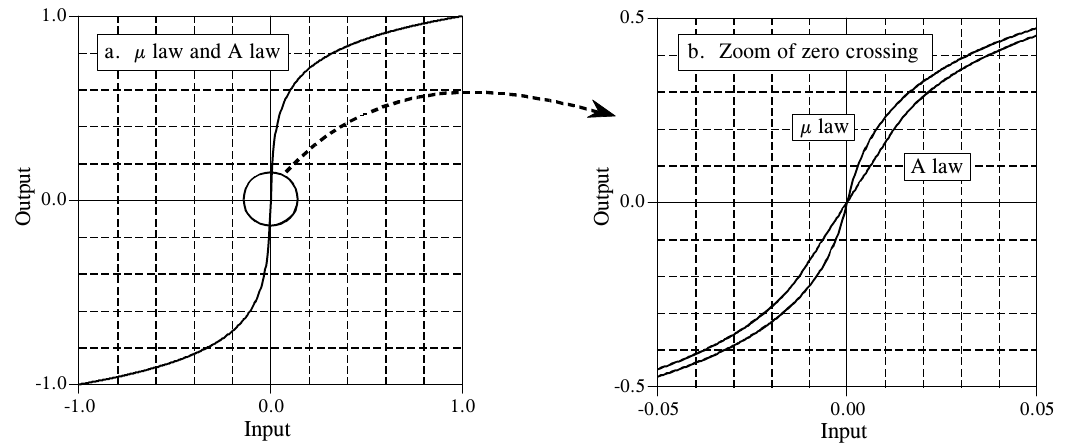
\includegraphics[width=0.892\linewidth,height=0.8\textheight,keepaspectratio]{assets/ch22/fig22-07.png}
\caption*{\textbf{图 22-7　压扩曲线。} µ255 律和 A
律的压扩曲线几乎完全相同，只在原点附近有差别。压扩在信号小的时候放大幅度，在信号大的时候减小幅度。
（a. µ law and A law = µ 律与 A 律；b. Zoom of zero crossing =
过零点附近放大。Input = 输入，Output = 输出。）}
\end{figure}

对模拟电子电路来说，做出一个稳定的非线性是件难事。一种方法是利用 PN
二极管结上电流与电压之间的对数关系，再加上电路来校正可怕的温度漂移。大多数压扩电路采用另一种策略：用一组直线段来近似这个非线性。一种典型方案是用
16 段直线来近似对数曲线，这些直线段叫弦(chord)。8
位输出的第一位表示输入是正还是负。接下来三位指出用的是 8 段正弦段或 8
段负弦段中的哪一段。最后四位把每段弦等分成 16
份。和大多数集成电路一样，压扩芯片的内部设计复杂且是专有的。与其操心芯片内部在干什么，不如把注意力放在引脚定义和规格书上。

\begin{quote}
\textbf{译注：} 原书把这些直线段拼成 cords（绳索），通行的术语是
chords（弦）。
\end{quote}

\section{语音合成与识别}

用计算机生成和识别语音是很难的问题；人们尝试了许多方法，成效都一般。这是
DSP
一个活跃的研究领域，无疑在今后许多年里也仍将如此。如果你指望这一节讲怎样搭建语音合成和识别电路，你会非常失望。这里只能简要介绍一下典型的方法。在开始之前应当指出，大多数能发出像人一样声音的商业产品并不是合成语音，而只是播放一段数字录制的真人语音。这种方法音质很好，但只限于预先录好的词语和短语。

几乎所有的语音合成与识别技术，都基于图 22-8
所示的人类发声模型。人的大多数语音可以分为浊音(voiced)和擦音(fricative)两类。浊音是空气从肺部被压出，经过声带(vocal
cords)，再从口和/或鼻出来时产生的。声带是喉结正后方横跨气流的两片薄薄的组织。随着肌肉张力的变化，声带以
50 到 1000 Hz
之间的频率振动，使一股股周期性的气流注入喉咙。元音就是浊音的例子。在图
22-8 中，浊音用脉冲串发生器表示，音高（即波形的基频）是一个可调参数。

\begin{figure}[htbp]
\centering
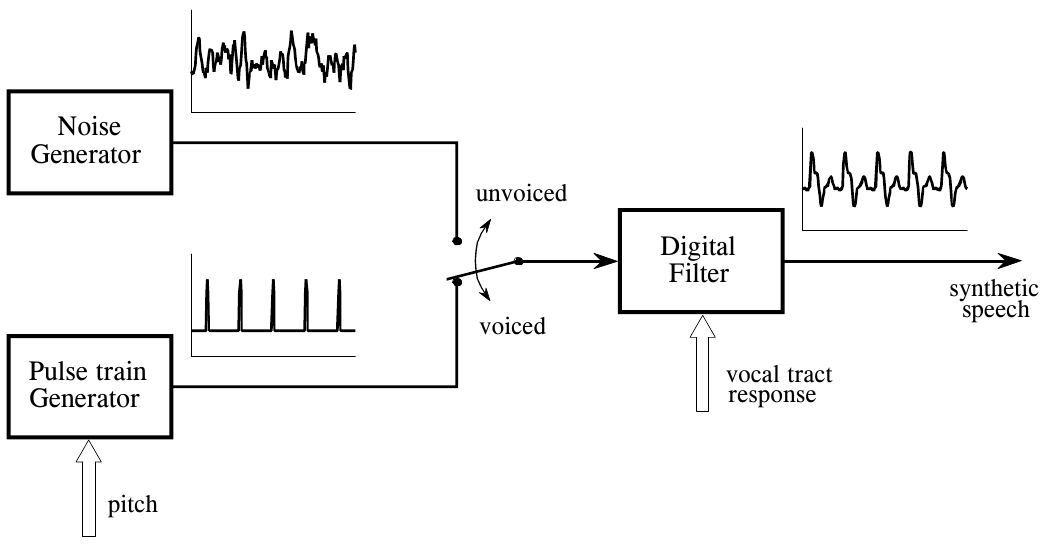
\includegraphics[width=0.867\linewidth,height=0.8\textheight,keepaspectratio]{assets/ch22/fig22-08.png}
\caption*{\textbf{图 22-8　人类发声模型。} 在一小段时间内（约 2 到 40
毫秒），语音可以用三个参数来建模：(1) 选择周期激励还是噪声激励；(2)
周期激励的音高；(3) 一个模仿声道响应的递归线性滤波器的系数。 （Noise
Generator = 噪声发生器，Pulse train Generator = 脉冲串发生器，pitch =
音高，unvoiced = 清音，voiced = 浊音，Digital Filter = 数字滤波器，vocal
tract response = 声道响应，synthetic speech = 合成语音。）}
\end{figure}

相比之下，擦音源于随机噪声，而不是声带的振动。当气流几乎被舌、唇和/或齿堵住，在收窄处附近产生湍流时，就会出现擦音。擦音包括
s、f、sh、z、v 和 th。在图 22-8 的模型中，擦音用噪声发生器表示。

这两种声源都要经过由舌、唇、口腔、咽喉和鼻腔形成的声学空腔的修饰。由于声音在这些结构中的传播是线性过程，可以用一个冲激响应选得合适的线性滤波器来表示。大多数情况下，模型中用的是递归滤波器，由递归系数决定滤波器的特性。由于这些声学空腔的尺寸有几厘米，频率响应主要是千赫兹范围内的一系列共振。在音频处理的行话里，这些共振峰叫共振峰频率(formant
frequencies)。改变舌和唇的相对位置，共振峰频率的频率和幅度都会随之改变。

\begin{quote}
\textbf{译注：} 原书把 formant frequencies 误拼成 format frequencies。
\end{quote}

图 22-9 是显示语音信号的一种常用方式：语谱图(voice
spectrogram)，也叫声纹(voiceprint)。把音频信号分成很短的段，比如 2 到 40
毫秒，用 FFT
求出每一段的频谱。把这些频谱并排放在一起，转换成灰度图像（幅度低的变浅，幅度高的变深）。这提供了一种图形化的方式，观察语音的频率成分怎样随时间变化。段的长度要在频率分辨率（段越长越好）和时间分辨率（段越短越好）之间折中。

\begin{figure}[htbp]
\centering
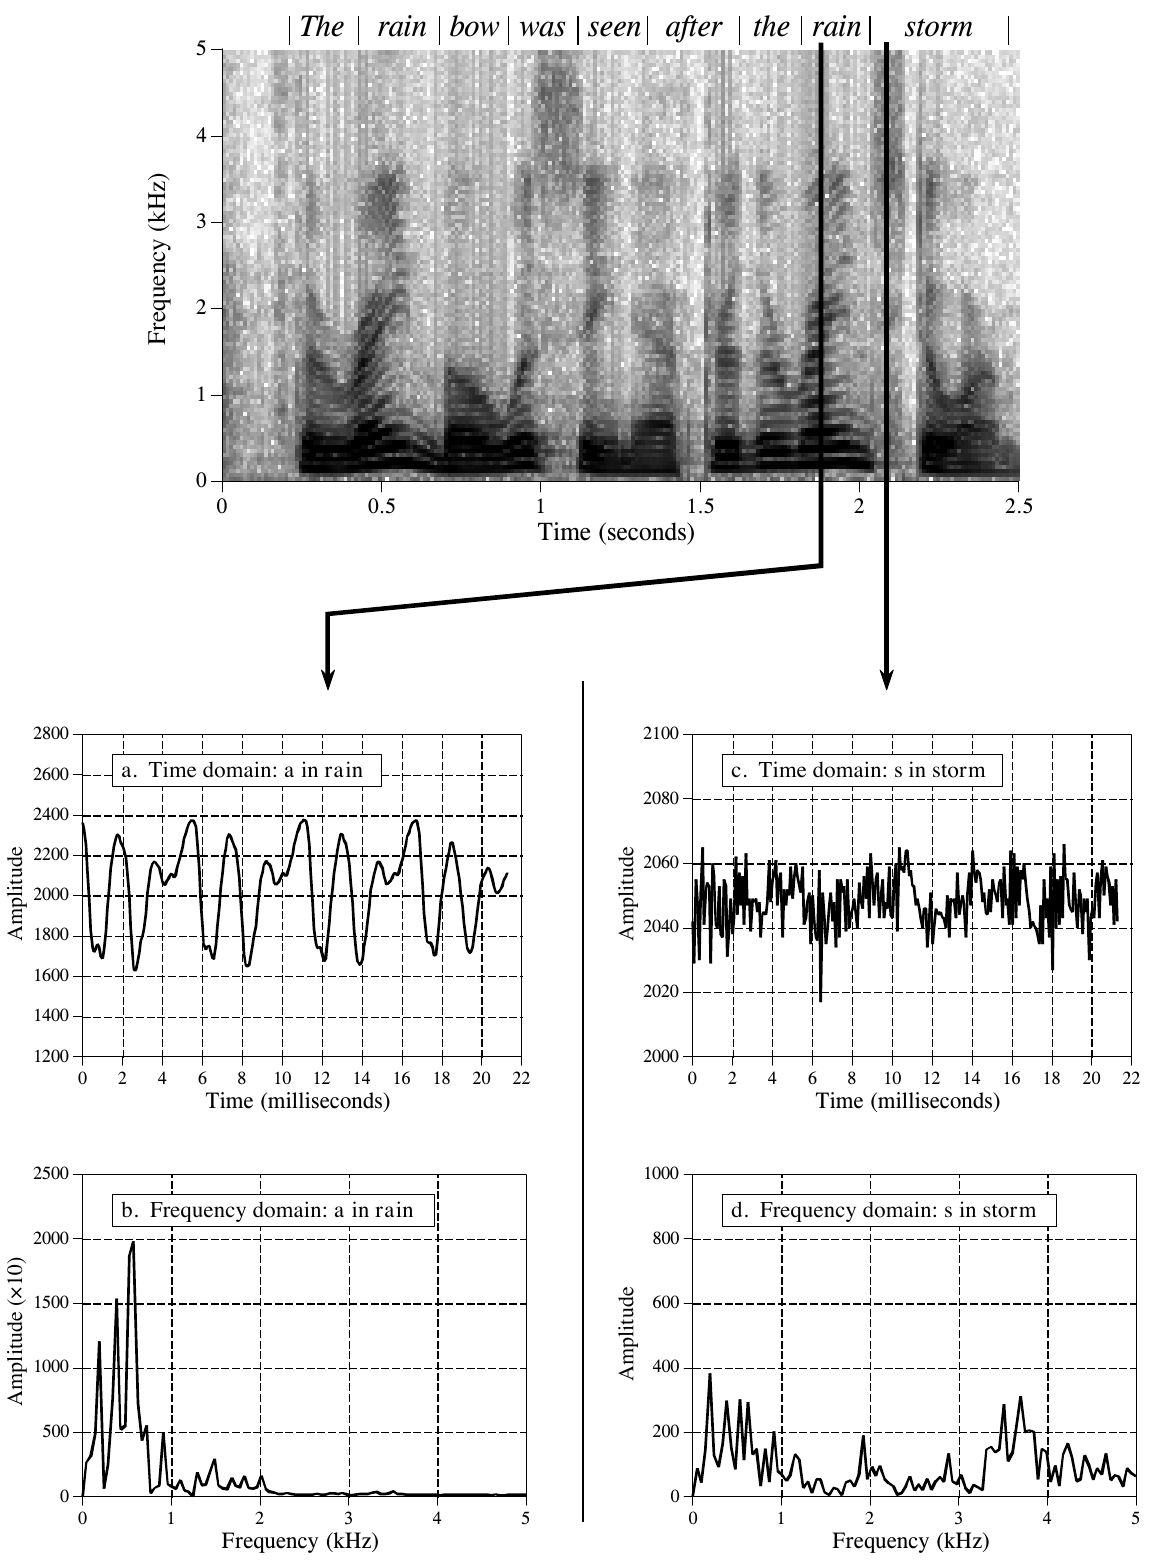
\includegraphics[width=0.958\linewidth,height=0.8\textheight,keepaspectratio]{assets/ch22/fig22-09.png}
\caption*{\textbf{图 22-9　语谱图。} 短语 ``The rainbow was seen after the rain
storm.''（雨后看到了彩虹）的语谱图。(a) 和 (b) 是 rain 中浊音 a
的时域和频域信号。(c) 和 (d) 是 storm 中擦音 s 的时域和频域信号。
（Frequency (kHz) = 频率（千赫），Time (seconds) = 时间（秒）；a. Time
domain: a in rain = 时域：rain 中的 a；b. Frequency domain: a in rain =
频域：rain 中的 a；c.~Time domain: s in storm = 时域：storm 中的
s；d.~Frequency domain: s in storm = 频域：storm 中的 s。Amplitude =
幅度，Amplitude (×10) = 幅度（×10），Time (milliseconds) =
时间（毫秒）。）}
\end{figure}

正如 rain 中的 a 所示，浊音的时域波形是周期的，如
(a)；频谱是一串等间距的谐波，如 (b)。相比之下，storm 中的 s
表明，擦音的时域信号是噪声状的，如 (c)；频谱也是噪声状的，如
(d)。这些频谱还显示出两种声音都受到共振峰频率的塑造。还要注意，rain
这个词说了两次，两次的时频图看起来很相似。

在一小段时间内（比如 25 毫秒），语音信号可以通过指定三个参数来近似：(1)
选择周期激励还是随机噪声激励；(2)
周期波的频率（如果用周期激励的话）；(3)
用来模仿声道响应的数字滤波器的系数。以每秒约 40
次的频率不断更新这三个参数，就能合成连续的语音。这种方法造就了 DSP
早期的商业成功之一：Speak \&
Spell（``说与拼''），一种广为销售的儿童电子学习机。这类语音合成的音质很差，听起来很机械，不太像人。不过它需要的数据率很低，通常只有几
k 位/秒。

这也是线性预测编码(LPC)语音压缩方法的基础。把数字录制的人类语音分成很短的段，每一段都按模型的三个参数来刻画。这通常每段需要大约一打字节，即每秒
2 到 6 k 字节。各段的信息按需要传输或存储，然后用语音合成器重建。

\begin{quote}
\textbf{译注：} 原书此处写 ``2 to 6 kbytes/sec''，与本章前文和表 22-2 的
2～6 k 位/秒不一致。按每段约 12 字节、每秒约 40 段计算，约为 0.5 k
字节/秒，即约 4 k 位/秒，应以''k 位/秒''为准。
\end{quote}

语音识别算法更进一步，试图在提取出的参数中识别模式。这通常需要把各段的信息与预先存储的声音模板进行比较，以求认出说的是哪些词。问题是，这种方法效果不太好。它对某些应用有用，但远远比不上人类听者的能力。要理解为什么语音识别对计算机来说这么难，设想有人突然说出下面这句话：

\begin{quote}
Larger run medical buy dogs fortunate almost when.（逐词直译：``更大 跑
医疗的 买 狗 幸运的 几乎 当\ldots\ldots 时''。）
\end{quote}

当然，你不会明白这句话的意思，因为它根本没有意思。更重要的是，你很可能连说出的每个词都听不全。这正是人类感知和理解语音方式的基本特点。词语是靠它们的声音识别的，但也靠句子的上下文和听者的预期。例如，设想听到下面两句话：

\begin{quote}
The child wore a spider ring on
Halloween.（孩子在万圣节戴了一枚蜘蛛戒指。）

He was an American spy during the war.（他在战争期间是一名美国间谍。）
\end{quote}

\begin{quote}
\textbf{译注：} 原书两句中加下划线的部分分别是 spider ring 和 spy
during，两者发音几乎相同。
\end{quote}

即使用来传达划线词语的声音完全相同，听者也会根据上下文听出正确的词。凭着你积累的关于世界的知识，你知道孩子不会''戴''特工，人也不会在战时变成吓人的首饰。这通常不是有意识的行为，而是人类听觉固有的一部分。

大多数语音识别算法只依赖单个词的声音，而不依赖上下文。它们试图识别词语，而不是理解语音。这使它们与人类听者相比处于极大的劣势。语音识别系统中常见三种令人烦恼的限制：(1)
被识别的语音必须在词与词之间有明显的停顿。这样算法就不必处理那些听起来相似、却由不同的词组成的短语（比如
spider ring 和 spy during）。对于习惯连贯说话的人来说，这既慢又别扭。(2)
词汇量往往只限于几百个词。这意味着算法只需在有限的集合中搜索最佳匹配。词汇量越大，识别时间和错误率都会增加。(3)
算法必须针对每个说话人进行训练。这需要每个使用系统的人把每个待识别的词说一遍，通常要重复五到十次。这种个性化的数据库大大提高了词语识别的准确率，但既不方便又费时间。

开发出成功的语音识别技术，回报是巨大的。语音是人类最快、最有效的交流方式。语音识别有可能取代书写、打字、键盘输入，以及由开关和旋钮提供的电子控制。它只需要再好用一点，就能被商业市场接受。语音识别的进步很可能既来自
DSP
本身，也同样来自人工智能和神经网络领域。别把这看作技术上的困难，把它看作技术上的机遇。

\section{非线性音频处理}

数字滤波能在许多方面改善音频信号。例如，维纳滤波(Wiener
filtering)可以把主要是信号的频率与主要是噪声的频率分开（见第 17
章）。同样，反卷积(deconvolution)可以补偿不想要的卷积，比如修复老录音（也在第
17 章讨论）。这类线性技术是 DSP
的支柱。还有几种非线性技术对音频处理也很有用。这里简要介绍其中两种。

第一种非线性技术用来降低语音信号中的宽带噪声。这类噪声包括：磁带嘶声、模拟电路中的电子噪声、风吹过话筒的声音、人群欢呼声等。线性滤波在这里没什么用，因为噪声的频率与语音信号的频率完全重叠，两者都覆盖
200 Hz 到 3.2 kHz
的范围。两个信号在时域和频域都重叠时，怎样才能把它们分开？

做法是这样的。在一小段语音中，各频率成分的幅度极不均匀。例如，图 22-10a
是一段 16 毫秒语音（即 8 kHz 采样率下的 128
个采样）的频谱。大部分信号集中在少数几个幅度大的频率上。相比之下，(b)
是只有随机噪声时的频谱；它非常不规则，但分布得更均匀，幅度也低。

\begin{figure}[htbp]
\centering
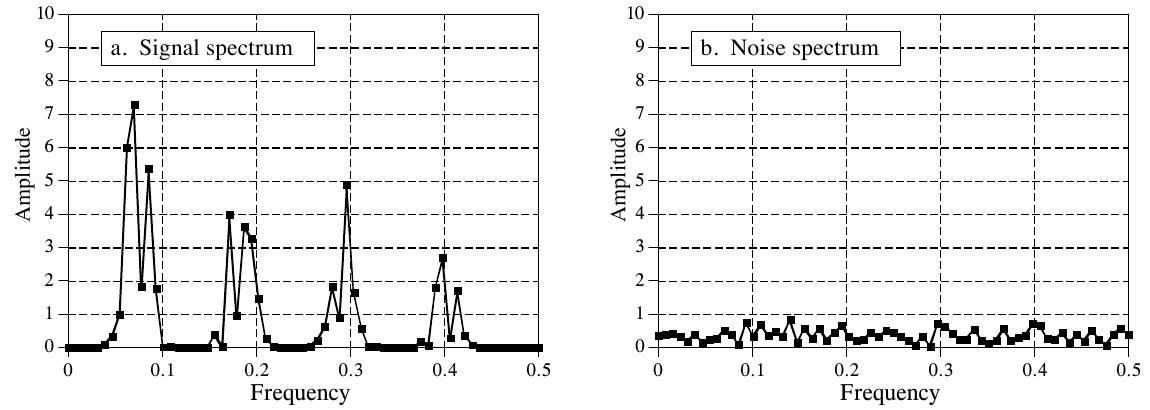
\includegraphics[width=0.958\linewidth,height=0.8\textheight,keepaspectratio]{assets/ch22/fig22-10.png}
\caption*{\textbf{图 22-10　语音和噪声的频谱。}
语音和噪声的频谱一般是重叠的，但如果信号段取得足够短，两者就会有一定程度的分离。(a)
是一段 16
毫秒语音的频谱，显示在这一特定段中，许多频率几乎不携带语音信息。(b)
是一个随机噪声源的频谱，所有分量的幅度都很小。（这些图不是真实信号，而是为了说明降噪技术画的示意图。）
（a. Signal spectrum = 信号频谱；b. Noise spectrum = 噪声频谱。Amplitude
= 幅度，Frequency = 频率。）}
\end{figure}

现在是关键的概念：如果信号和噪声同时存在，可以通过查看每个频率的幅度把两者部分地分开。如果幅度大，它很可能主要是信号，因此应当保留。如果幅度小，可以认为它主要是噪声，因此应当丢弃，即设为零。中等大小的频率分量在这两个极端之间以某种平滑的方式调整。

看待这种技术的另一种方式，是把它当作一个时变的维纳滤波器。你应该还记得，维纳滤波器的频率响应让主要是信号的频率通过，拒绝主要是噪声的频率。这需要预先知道信号和噪声的频谱，才能确定滤波器的频率响应。这种非线性技术用的是同样的思想，只是维纳滤波器的频率响应针对每一段、根据该段的频谱重新计算。换句话说，滤波器的频率响应逐段变化，由信号本身的特性决定。

实现这种（以及其他）非线性技术的困难之一，是用来对长信号滤波的重叠相加法(overlap-add
method)不再有效。由于频率响应在变化，各段的时域波形不再与相邻段对齐。要克服这一点，可以记住：音频信息编码在随时间变化的频率模式中，而不是在时域波形的形状中。一种典型做法是把原来的时域信号分成相互重叠的段。处理之后，在重新合并之前给每个重叠段加一个平滑的窗。这样频谱从一段到下一段就能平滑过渡。

第二种非线性技术叫同态信号处理(homomorphic signal
processing)。这个术语的字面意思是''相同的结构''。噪声和干扰与有用信号的结合方式不只有相加；相乘和卷积也是信号混合的常见方式。如果信号以非线性方式（即相加以外的任何方式）结合，就无法用线性滤波把它们分开。同态技术试图把问题变成线性的，从而分开以非线性方式结合的信号。也就是说，把问题转换成与线性系统相同的结构。

例如，考虑一个经由 AM
无线电波传输的音频信号。随着大气条件的变化，接收到的信号幅度时大时小，使接收到的音频信号的响度随时间缓慢变化。这可以建模为音频信号
a{[} {]} 乘以一个缓慢变化的信号 g{[}
{]}，后者代表不断变化的增益。这个问题通常用一种叫自动增益控制(automatic
gain control，AGC)的电子电路来处理，但也可以用非线性 DSP 来校正。

如图 22-11 所示，输入信号 a{[} {]}×g{[} {]} 通过对数函数。根据恒等式
\(\log(x \times y) = \log x + \log y\)，得到两个以相加方式结合的信号，即
log a{[} {]} + log g{[}
{]}。换句话说，对数就是把相乘这个非线性问题变成相加这个线性问题的同态变换。

\begin{quote}
\textbf{译注：} 原书这个恒等式印成了 log(x + y) = log x + log y，应为
log(x × y)。
\end{quote}

\begin{figure}[htbp]
\centering
\includegraphics[width=0.875\linewidth,height=0.8\textheight,keepaspectratio]{assets/ch22/fig22-11.png}
\caption*{\textbf{图 22-11　相乘信号的同态分离。}
对输入信号取对数，把相乘的分量变成相加的分量。然后可以用线性滤波把这些分量分开，再撤销对数的作用。
（Logarithm = 对数，Linear Filter = 线性滤波器，Anti-Logarithm =
反对数。）}
\end{figure}

接下来，用常规的线性滤波器把相加的信号分开，也就是让一些频率通过、拒绝另一些频率。对于
AGC，增益信号 g{[} {]} 由非常低的频率组成，远低于语音信号 200 Hz 到 3.2
kHz
的频带。这些信号取对数后的频谱会更复杂，但思路是一样的：用一个高通滤波器把变化的增益分量从信号中去掉。

实际上，log a{[} {]} + log g{[} {]} 被变成了 log a{[}
{]}。最后一步，用指数函数（反对数，即
\(e^x\)）撤销对数，得到所需的输出信号 a{[} {]}。

图 22-12
是一个分离卷积信号的同态系统。这已被证明有用的一个应用是去除音频信号中的回声。也就是说，音频信号与一个由''冲激函数加上一个平移并缩放过的冲激函数''构成的冲激响应卷积在了一起。卷积的同态变换由两级组成：先做傅里叶变换，把卷积变成相乘；再取对数，把相乘变成相加。和前面一样，接着用线性滤波把信号分开，再撤销同态变换。

\begin{figure}[htbp]
\centering
\includegraphics[width=1.000\linewidth,height=0.8\textheight,keepaspectratio]{assets/ch22/fig22-12.png}
\caption*{\textbf{图 22-12　卷积信号的同态分离。}
先做傅里叶变换再取对数，把卷积在一起的分量变成相加的分量。用线性滤波分开这些相加的分量之后，再按原来的步骤逐一撤销。
（Homomorphic Transform = 同态变换，Inverse Homomorphic Transform =
逆同态变换，Fourier Transform = 傅里叶变换，Logarithm = 对数，Linear
Filter = 线性滤波器，Anti-Logarithm = 反对数，Inverse Fourier Transform
= 逆傅里叶变换；x{[} {]} \dspsym{∗} y{[} {]} 中的 \dspsym{∗} 是卷积。）}
\end{figure}

图 22-12
有一个有趣的转折：线性滤波处理频域信号的方式，和通常处理时域信号的方式一样。换句话说，时域和频域的角色与平常互换了。例如，如果用
FFT
卷积来完成线性滤波这一级，被相乘的''频谱''就会位于时域。这种角色反转催生了一套奇怪的行话。例如，倒谱(cepstrum，把
spectrum
的字母重新排列而成)是傅里叶变换的对数的傅里叶变换。同样，有长通(long-pass)和短通(short-pass)滤波器，而不是低通和高通滤波器。有些作者甚至使用''倒频分析''(Quefrency
Alanysis，由 Frequency Analysis 换字母而来)和''倒滤波''(liftering，由
filtering 换字母而来)这样的说法。

请记住，这些只是对复杂 DSP
算法的简化描述；同态处理充满了微妙的细节。例如，对数必须能处理输入信号中的负值和正值，因为音频信号就有这个特点。这需要用到复对数(complex
logarithm)，它比日常科学和工程中用的对数更高深。如果把线性滤波限制为零相位滤波器，复对数可以通过对信号的绝对值取普通对数求得。通过零相位滤波器之后，再把原信号的符号重新加到滤波后的信号上。

另一个问题是取对数时出现的混叠。例如，设想对一个连续正弦波做数字化。根据采样定理，每个周期两个或更多采样就够了。现在考虑对这个连续正弦波的对数做数字化。它的尖角需要每个周期多得多的采样才能把波形捕捉下来，也就是防止混叠。取对数之后所需的采样率很容易达到之前的
100
倍。而且，对数是作用在连续信号上还是它的数字表示上，结果都一样。除非采样率高到能捕捉非线性产生的尖角，否则就会发生混叠。结果是音频信号可能需要以
100 kHz 或更高的频率采样，而不是标准的 8 kHz。

即使处理好了这些细节，也不能保证线性化后的信号可以被线性滤波器分开。这是因为即使原信号的频谱不重叠，线性化后信号的频谱也可能重叠。例如，设想把两个正弦波相加，一个
1 kHz，一个 2
kHz。由于这两个信号在频域中不重叠，可以用线性滤波把它们完全分开。现在设想把这两个正弦波相乘。用同态处理，对组合后的信号取对数，得到一个正弦波的对数加上另一个正弦波的对数。问题是，正弦波的对数含有许多谐波。由于两个信号的谐波相互重叠，不可能把它们完全分开。

尽管有这些障碍，同态处理教给我们一个重要的道理：处理信号的方式应当与信号形成的方式相一致。换句话说，任何
DSP 任务的第一步，都是弄清信息在所处理的信号中是怎样表示的。

% !TEX root = ../main.tex
% 本文件由 build-tex.sh 从 23-DSP指南-第23章中译.md 生成，改内容请改 md 后重新生成

\chapter{图像的形成与显示}\label{ch-23}

图像描述的是某个参数在一个面上如何变化。例如，普通的可见光图像来自光强在二维平面上的变化。不过，科学成像用的参数并不只有光。例如，图像可以由集成电路的温度、病人动脉中的血流速度、遥远星系发出的
X
射线、地震时的地面运动等构成。这些特殊的图像通常会被转换成普通的图片（即光学图像），以便用人眼来判读。作为图像处理的第一章，本章介绍数字图像是怎样形成、又是怎样呈现给观察者的。

\section{数字图像的结构}

图 23-1
展示了数字图像的结构。这幅示例图像是金星，由环绕它飞行的空间探测器用微波雷达拍摄。之所以要用微波成像，是因为金星浓密的大气挡住了可见光，普通照相根本行不通。图中的图像由
40,000 个采样组成，排成 200 列 × 200
行的二维数组。和一维信号一样，这些行和列可以编号为 0 到
199，也可以编号为 1 到
200。按图像处理的行话，每个采样叫做一个像素(pixel)，是 picture
element（图像元素）的缩写。本例中每个像素是一个 0 到 255
之间的数。拍摄时，这个数对应行星表面相应位置反射回来的微波能量的多少。为了把它显示成可见的图像，每个像素的值被转换成一个灰度(grayscale)：0
是黑，255 是白，中间的值是深浅不同的灰。

\begin{figure}[htbp]
\centering
\includegraphics[width=0.996\linewidth,height=0.8\textheight,keepaspectratio]{assets/ch23/fig23-01.png}
\caption*{\textbf{图 23-1　数字图像的结构。}
这幅示例图像是以反射微波观察到的金星。数字图像用一个二维数组表示，数组里的每个数叫做一个像素。本图中数组为
200 行 × 200 列，每个像素是 0 到 255
之间的一个数。拍摄时，每个像素的值对应反射回来的微波能量的强弱。把
0～255 的每个值对应到深浅不同的灰色，就形成了灰度图像。 （Column =
列，Row = 行。左上是整幅图，右上是方框区域（第 50～65 行、第 150～165
列）放大后的像素格，下方是这些像素的数值。原书图注排在图左下，裁图时已去掉，译文见上。）}
\end{figure}

图像的信息编码在空间域(spatial
domain)中，空间域相当于图像版的时域。换句话说，图像中的特征是用边缘(edge)来表示的，而不是用正弦波。这意味着像素的间距和数量，取决于需要看清多小的特征，而不是取决于采样定理的形式约束。图像中也会出现混叠(aliasing)，但它一般被看作一种小麻烦，而不是大问题。例如，细条纹西装在电视上看起来很糟糕，因为这种重复图案的频率超过了奈奎斯特频率(Nyquist
frequency)。混叠出来的频率表现为明暗相间的条带，随着人的走动在衣服上移动。

一幅''典型''的数字图像大约由 500 行 × 500
列组成。这是电视、个人计算机应用和一般科研中常见的图像质量。像素更少的图像，比如
250 ×
250，被认为分辨率异常低。新出现的成像方式往往就是这样；随着技术成熟，像素会越来越多。这种低分辨率图像看起来明显不自然，常常能看到一个个像素。另一端，超过
1000 × 1000 像素的图像被认为质量特别好，这是最好的计算机图形、高清电视和
35
毫米电影的质量。还有一些应用需要更高的分辨率，每边几千个像素：数字化的 X
光片、太空照片，以及杂志上的光面广告。

使用较低分辨率图像最大的动力在于要处理的像素更少。这不是小事；图像处理中最难的问题之一，就是管理海量的数据。例如，一秒钟的数字音频大约需要
8 千字节，而一秒钟的电视大约需要 8 兆字节。用 33.6 kbps
的调制解调器传送一幅 500 × 500 像素的图像，要将近一分钟！图像尺寸跳到
1000 × 1000，这些问题就翻两番。

\begin{quote}
\textbf{译注：} ``一秒钟数字音频约 8 千字节''对应的是电话质量（8 kHz
采样、每采样 8 位）；CD 音质（44.1 kHz、16 位、立体声）约为每秒 176
千字节。
\end{quote}

图像处理中通常用 256
个灰度级（量化级），对应每像素一个字节。这样做有几个原因。第一，单个字节便于数据管理，因为计算机通常就是这样存储数据的。第二，图像中像素数量巨大，这在一定程度上弥补了量化级数的不足。例如，设想一组相邻像素的值在数字编号（digital
number，DN）145 和 146 之间交替。人眼会把这片区域感知为亮度
145.5。换句话说，图像本身带有很强的抖动(dithering)效果。第三，也是最重要的一点：1/256（0.39\%）的亮度步长，比人眼能察觉的还小。呈现给人看的图像，用超过
256 级也不会变得更好。

不过，有些图像需要以每像素超过 8 位的精度来存储。记住，DSP
中遇到的大多数图像表示的是非视觉参数。采集到的图像可能需要更多的量化级，才能恰当地捕捉信号的细微之处。重点在于：不要指望人眼能看出这些细密的级别中包含的全部信息。后面讨论亮度和对比度时，我们会考虑怎样绕开这个问题。

数字图像中每个像素的值，代表被数字化的连续图像中的一小块区域。例如，设想金星探测器在环绕飞行时，沿行星表面每隔
10 米取一个样。这就定义了一个方形的采样间距和采样网格(sampling
grid)，每个像素代表一块 10 米 × 10
米的区域。现在设想一次微波反射测量中发生了什么。探测器发出一束高度聚焦的微波能量，照到地面上的，比如说，是一块直径
15
米的圆形区域。因此，不管采样网格多大，每个像素所含的都是这块圆形区域的信息。

连续图像中对像素值有贡献的这块区域，叫做采样孔径(sampling
aperture)。采样孔径的大小通常与所用成像系统的固有能力有关。例如，显微镜受光学元件质量和光波长的限制，电子相机受图像传感器中电子随机扩散的限制，等等。大多数情况下，采样网格做得与系统的采样孔径大致相同。最终数字图像的分辨率，主要受这两者中较大的那个限制：采样网格或采样孔径。第
25 章讨论数字图像的空间分辨率时，我们会回到这个话题。

给数字图像加上颜色的办法，是每个像素用三个数，分别表示三种原色------红、绿、蓝------的强度。混合这三种颜色可以产生人眼能感知的所有颜色。每种颜色的强度通常用一个字节存储，于是图像总共能表示
256×256×256 = 1680 万种不同的颜色。

当目的是向观众呈现世界的真实画面时，比如电视和照片，颜色非常重要。但科学和工程中的图像通常不是这样用的。这里的目的是把人的视觉系统当作工具，去分析一个二维信号。黑白图像就足够了。

\section{相机与眼睛}

眼睛的结构和工作方式与电子相机非常相似，放在一起讨论很自然。两者都基于两个主要部件：镜头组件和成像传感器(imaging
sensor)。镜头组件收集物体发出的一部分光，把它聚焦到成像传感器上。成像传感器再把光的图案转换成视频信号，可能是电信号，也可能是神经信号。

图 23-2
展示了透镜的工作方式。在这个例子中，一位滑冰者的像被聚焦到一块屏幕上。聚焦(focus)的意思是：滑冰者身上的每一点，都与屏幕上的一个对应点一一对应。例如，考虑脚尖上
1 mm × 1 mm 的一块区域。在明亮的光线下，每秒大约有 100
万亿个光子打到这一平方毫米上。根据表面性质的不同，这些入射光子中有 1\%
到 99\%
会被反射到随机的方向。被反射的光子中只有很小一部分会穿过透镜。例如，一个距离物体
3 米、直径 1 厘米的透镜，只能接收到大约百万分之一的反射光。

\begin{figure}[htbp]
\centering
\includegraphics[width=0.821\linewidth,height=0.8\textheight,keepaspectratio]{assets/ch23/fig23-02.png}
\caption*{\textbf{图 23-2　透镜的聚焦。}
透镜收集从一个点光源发散出来的光，迫使它们在另一个位置重新会聚成一个点。这使得透镜能把像投射到一个面上。
（lens = 透镜，projected image = 投射的像。）}
\end{figure}

透镜中的折射(refraction)会改变每个光子的方向，改变多少取决于光子打到玻璃/空气界面的位置和角度。这些方向变化使得从一个点发散出去的光，在投影屏上重新会聚到一个点。从脚尖反射并穿过透镜的所有光子，都在投射的像中的''脚尖''处重新汇合。同理，物体上任何一点发出的光，都有一部分会穿过透镜，并聚焦到投射的像中的对应点。

图 23-3 和图 23-4
分别画出了电子相机和人眼的主要结构。两者都是不透光的外壳，一端装着透镜，另一端是图像传感器。相机里充满空气，而眼睛里充满透明液体。每个透镜系统都有两个可调参数：焦距和光圈(iris)直径。

\begin{figure}[htbp]
\centering
\includegraphics[width=0.508\linewidth,height=0.8\textheight,keepaspectratio]{assets/ch23/fig23-03.png}
\caption*{\textbf{图 23-3　电子相机示意图。}
聚焦是通过让镜头靠近或远离成像传感器来实现的。到达传感器的光量由光圈控制，光圈是一个改变镜头有效直径的机械装置。当今相机中最常见的成像传感器是
CCD，即一个由感光元件组成的二维阵列。 （iris = 光圈，focus = 调焦，lens
= 镜头，CCD = 电荷耦合器件，serial output =
串行输出。原书图注排在图左侧，裁图时已去掉，译文见上。）}
\end{figure}

\begin{figure}[htbp]
\centering
\includegraphics[width=0.492\linewidth,height=0.8\textheight,keepaspectratio]{assets/ch23/fig23-04.png}
\caption*{\textbf{图 23-4　人眼示意图。} 眼睛是一个充满液体、直径约 3
厘米的球体，外面包着一层坚韧的外壳，叫巩膜。聚焦主要由角膜完成，角膜是眼睛前部一个固定的透镜。焦距的调节靠收缩连在眼内柔性晶状体上的肌肉来实现。进入眼睛的光量由虹膜控制，虹膜由不透明的肌肉组织构成，遮住晶状体的一部分。眼球的后半球是视网膜，这是一层感光神经细胞，把像转换成视神经中的神经信号。
（sclera = 巩膜，ciliary muscle = 睫状肌，iris = 虹膜，clear liquid =
透明液体，lens = 晶状体，cornea = 角膜，fovea = 中央凹，retina =
视网膜，optic nerve = 视神经，TO EAR = 朝耳朵，TO NOSE = 朝鼻子，top
view = 俯视图。原书图注排在图左侧，裁图时已去掉，译文见上。）}
\end{figure}

如果透镜没有正确聚焦，物体上的每一点都会投射到成像传感器上的一个圆形区域，使像变模糊。在相机中，聚焦是靠物理地移动镜头、使它靠近或远离成像传感器来实现的。相比之下，眼睛里有两个透镜：眼球前部的一个凸起，叫角膜(cornea)；以及眼内一个可调的透镜，即晶状体。光的折射大部分由角膜完成，但角膜的形状和位置是固定的。焦距的调节由内部的晶状体完成，它是一种柔性结构，可以在睫状肌(ciliary
muscle)的作用下变形。这些肌肉收缩时，晶状体变扁，使物体清晰成像。

\begin{quote}
\textbf{译注：}
原书此处说''肌肉收缩时晶状体变扁''。按目前生理学的通常解释，睫状肌收缩时悬韧带放松，晶状体变得更凸（用于看近处）；睫状肌放松时晶状体被拉扁（用于看远处）。译文照原书翻译，供参考。
\end{quote}

在两种系统中，光圈都用来控制透镜有多少面积暴露在光下，从而控制投射到成像传感器上的像的亮度。眼睛的虹膜(iris)由不透明的肌肉组织构成，收缩时会使瞳孔(pupil，即透光的开口)变大。相机的光圈则是完成同样功能的机械组件。

光学系统中的各个参数会以许多意想不到的方式相互影响。例如，考虑可用光量和光传感器的灵敏度怎样影响所得图像的清晰度。之所以有影响，是因为光圈直径和曝光时间要调节到恰好把适量的光从景物传到图像传感器上。如果光线充足，就可以缩小光圈直径，从而得到更大的景深(depth-of-field，即物体保持清晰的那段距相机的距离范围)。当物体处于不同距离时，更大的景深能给出更清晰的图像。此外，光线充足还能缩短曝光时间，减少相机抖动和物体运动造成的模糊。光学系统中充满了这类取舍。

相机和眼睛都需要可调的光圈，因为环境中光强的范围远大于光传感器能直接处理的范围。例如，阳光和月光的光强相差大约一百万倍。再加上反射率可以在
1\% 到 99\% 之间变化，光强的范围就接近一亿倍。

电子相机的动态范围(dynamic range)通常是 300 到
1000，定义为器件能测量的最大信号除以器件的固有噪声。换句话说，产生的最大信号是
1 伏，而在黑暗中的均方根噪声约为 1
毫伏。典型的相机镜头，光圈能把通光面积改变约 300
倍。这使得典型电子相机的动态范围达到几十万。显然，在明亮阳光下用的相机和镜头组件，到了漆黑的夜里就没法用了。

相比之下，眼睛的动态范围几乎覆盖了环境中的巨大变化。出人意料的是，实现这一巨大动态范围的主要手段并不是虹膜。从暗到亮，瞳孔的面积只变化约
20
倍。剩下的动态范围，靠感光神经细胞逐渐调整自身的灵敏度来应付。例如，走进漆黑的电影院后，眼睛要花几分钟才能适应弱光。

DSP
改善图像的一种方法，是减小观察者需要面对的动态范围。也就是说，我们不希望同一幅图像中既有很亮的区域又有很暗的区域。一幅反射图像由两个图像信号构成：景物被照明的二维分布，乘以景物反射率的二维分布。反射率分布的动态范围小于
100，因为所有普通材料都反射入射光的 1\% 到
99\%。图像的大部分信息都包含在这里，比如物体在景物中的位置以及它们的表面特征。相比之下，照明信号取决于物体周围的光源，而不取决于物体本身。照明信号的动态范围可以达到几百万，不过在单幅图像中更典型的是
10 到
100。照明信号携带的有用信息很少，却会因为增大动态范围而使最终图像变差。DSP
可以通过抑制照明信号、让反射率信号在图像中占主导来改善这种情况。下一章会介绍实现这一算法的一种方法。

覆盖在眼球后部的感光表面叫视网膜(retina)。如图 23-5
所示，视网膜可以分成三层主要的特化神经细胞：一层把光转换成神经信号，一层做图像处理，一层把信息传给通向大脑的视神经(optic
nerve)。在几乎所有动物中，这些层的排列方向看起来都是反的。也就是说，感光细胞在最后一层，光要先穿过其他层才能被检测到。

\begin{figure}[htbp]
\centering
\includegraphics[width=0.908\linewidth,height=0.8\textheight,keepaspectratio]{assets/ch23/fig23-05.png}
\caption*{\textbf{图 23-5　人的视网膜。} 视网膜包含三个主要层次：(1)
视杆细胞和视锥细胞这两种感光器；(2) 中间层，负责数据压缩和图像处理；(3)
通向大脑的视神经纤维。这几层的结构看起来是反的，光要先穿过其他层才能到达感光器。
（optic nerve = 视神经，connecting layer = 连接层，rods and cones =
视杆细胞和视锥细胞，light = 光，optic nerve to brain =
通向大脑的视神经，sclera = 巩膜。原书图注中的 principle 应为
principal。）}
\end{figure}

检测光的细胞有两种：视杆细胞(rod)和视锥细胞(cone)，名字来自它们在显微镜下的外形。视杆细胞专门在光线很弱时工作，比如在夜空下。在接近全黑的环境中，视觉显得噪声很大，也就是说，像里布满了不断变化的颗粒状图案。这是因为图像信号非常弱，而不是眼睛本身的缺陷。进入眼睛的光太少了，以至于能看到单个光子的随机检测。这叫统计噪声(statistical
noise)，所有弱光成像中都会遇到，比如军用夜视系统。第 25
章会再讲这个话题。由于视杆细胞不能分辨颜色，弱光下的视觉是黑白的。

视锥细胞专门用来分辨颜色，但只有在光线较充足时才能工作。眼睛里有三种视锥细胞：对红光敏感的、对绿光敏感的和对蓝光敏感的。这是因为它们含有不同的感光色素(photopigment)，即吸收不同波长（颜色）光的化学物质。图
23-6 给出了能触发这三种感光器的光的波长。这叫 RGB
编码，颜色信息就是以这种形式通过视神经离开眼睛的。由于大脑低层的神经处理，人对颜色的感知变得更加复杂。RGB
编码被转换成另一种编码方案，把颜色分为：红或绿、蓝或黄、亮或暗。

\begin{figure}[htbp]
\centering
\includegraphics[width=0.471\linewidth,height=0.8\textheight,keepaspectratio]{assets/ch23/fig23-06.png}
\caption*{\textbf{图 23-6　眼睛的光谱响应。}
人眼中的三种视锥细胞分别对光谱的不同部分有响应，大致对应红、绿、蓝。这三者的组合构成了人能感知的所有颜色。视锥细胞的灵敏度不够，无法在弱光环境中工作，这时由视杆细胞来检测图像。这就是夜里难以分辨颜色的原因。
（Relative sensitivity = 相对灵敏度，Wavelength (nm) =
波长（纳米）；blue cones = 蓝视锥细胞，rods = 视杆细胞，green cones =
绿视锥细胞，red cones = 红视锥细胞；perception of wavelength =
对波长的感知：violet 紫、blue 蓝、green 绿、yellow 黄、orange 橙、red
红。原书图注排在图左侧，裁图时已去掉，译文见上。）}
\end{figure}

RGB
编码是人类视觉的一个重要局限：环境中存在的各种波长，被笼统地归入仅仅三大类。相比之下，专用相机能把光谱分成数百乃至数千种不同的颜色。例如，可以用它们把细胞分类为癌变或健康、了解遥远恒星的物理性质，或者发现藏在森林里的伪装士兵。为什么眼睛在分辨颜色方面如此有限？显然，人类生存所需的，只是在绿叶之间、蓝天背景下找到一个红苹果。

视杆细胞和视锥细胞大约 3 μm 宽，紧密地排满视网膜整个 3 cm × 3 cm
的表面。于是视网膜由大约 10,000 × 10,000 = 1
亿个感光器组成的阵列构成。相比之下，视神经只有大约一百万根神经纤维与这些细胞相连。平均来说，每根视神经纤维通过连接层与大约
100
个感光器相连。除了汇总信息，连接层还会增强图像：锐化边缘，并抑制景物中的照明成分。这种生物图像处理将在下一章讨论。

视网膜正中央有一小块区域，叫中央凹(fovea，拉丁语''凹坑''的意思)，用于高分辨率视觉（见图
23-4）。中央凹在几个方面与视网膜其他部分不同。第一，视神经和连接层被推到中央凹的两侧，让感光器更直接地暴露在入射光下。这使得中央凹看起来是视网膜上的一个小凹陷。第二，中央凹里只有视锥细胞，而且排列得比视网膜其他部分更紧密。中央凹里没有视杆细胞，这解释了为什么夜里看东西时，眼睛稍微偏向物体一侧往往比直视看得更清楚。第三，每根视神经纤维只受少数几个视锥细胞影响，因而定位能力很好。中央凹小得出奇。在正常阅读距离上，中央凹只能看到直径约
1 毫米的区域，比一个字母还小！这块区域内的分辨率大约相当于 20×20
的像素网格。

人的视觉靠一种叫扫视(saccade)的跳跃式眼动来弥补中央凹太小的缺陷。这些突然的运动让高分辨率的中央凹能快速扫过视野，寻找相关信息。此外，扫视使视杆细胞和视锥细胞面对的光图案不断变化。这一点很重要，因为视网膜天然会适应光强的变化。事实上，如果强迫眼睛一直盯着同一个景物不动，几秒钟后细节和颜色就开始消退。

电子相机中最常用的图像传感器是电荷耦合器件(charge coupled
device，CCD)。CCD 是一种集成电路，在 1980
年代取代了大部分真空管摄像机，就像二十年前晶体管取代了真空管放大器一样。CCD
的核心是一片薄薄的硅片，通常约 1 平方厘米。如图 23-7
的剖面图所示，背面镀有一层接地的薄金属。正面覆盖着一层很薄的电绝缘层，以及一组重复排列的电极。最常见的
CCD 是三相读出(three phase
readout)型，每隔两个电极连在一起（即每三个一组）。所用的硅叫 p
型硅，意思是它含有过量的正电荷载流子，叫空穴(hole)。在这里的讨论中，可以把空穴想成一个能在硅中自由移动的带正电的粒子。图中空穴用''+``号表示。

\begin{figure}[htbp]
\centering
\includegraphics[width=0.871\linewidth,height=0.8\textheight,keepaspectratio]{assets/ch23/fig23-07.png}
\caption*{\textbf{图 23-7　电荷耦合器件（CCD）的工作原理。} 如剖面图所示，一薄片 p
型硅上覆盖着一层绝缘层和一组电极。电极每三个连成一组，可以施加三路独立的电压：φ1、φ2
和
φ3。给某个电极加正电压时，空穴（即用''+``表示的正电荷载流子）被推开，形成一个缺少空穴的区域，叫势阱。入射光产生空穴和电子，使电子在每个势阱中积累起来（用''−``表示）。通过操纵三路电极电压，每个势阱中的电子可以被移到硅片边缘，在那里由一个电荷敏感放大器把电荷转换成电压。
（insulator = 绝缘层，electrode = 电极，well = 势阱，output amplifier =
输出放大器，grounded back surface = 接地的背面，p type silicon = p
型硅，light photon = 光子；φ1 (10v) 等表示各相电极上的电压。）}
\end{figure}

在 (a) 中，三相之一加上 +10 伏电压，另外两相保持 0
伏。这使得空穴从每隔两个的电极下方移开，因为正电荷会被正电压排斥。这就在这些电极下方形成了一个叫阱(well)的区域，是物理术语势阱(potential
well)的简称。

CCD 中的每个阱都是非常高效的光传感器。如 (b)
所示，一个光子打到硅上，它的能量转化为两个带电粒子：一个电子和一个空穴。空穴移走，留下电子困在阱里，被电极上的正电压束缚住。图中电子用''−``号表示。在积分期(integration
period)内，照到 CCD 上的光图案被转换成 CCD
各个阱中的电荷图案。光源越暗，需要的积分期越长。例如，标准电视的积分期是
1/60 秒，而天文摄影可以积累光好几个小时。

电子图像的读出方式相当巧妙：每个阱中积累的电子被推向输出放大器。如 (c)
所示，在两相电极线上加正电压，使每个阱都向右扩展。如 (d)
所示，下一步撤掉第一相的电压，原来的阱随之消失。这样，积累的电子就停留在比起始位置右移一格的阱中。在三相电极线之间重复这种脉冲序列，积累的电子就被一路推向右边，直到到达一个电荷敏感放大器(charge
sensitive
amplifier)。这是''一个电容后面接一个单位增益缓冲器''的花哨名字。电子从最后一个阱被推出时，流到电容上并产生一个电压。为了获得高灵敏度，电容做得极小，通常小于
1 pF。这个电容和放大器是 CCD 的组成部分，做在同一块硅片上。离开 CCD
的信号是一串电压电平，与依次各阱接收到的光量成正比。

图 23-8 展示了怎样从 CCD
读出二维图像。积分期结束后，每个阱中积累的电荷沿着列向上移动，一次移动一行。例如，第
15 行的所有阱先移到第 14 行，再到第 13 行，再到第 12
行，依此类推。每次各行上移时，第 1
行的所有阱都被转移到水平寄存器(horizontal
register)中。水平寄存器是一组特殊的 CCD
阱，能快速地沿水平方向把电荷移到电荷敏感放大器。

\begin{figure}[htbp]
\centering
\includegraphics[width=0.729\linewidth,height=0.8\textheight,keepaspectratio]{assets/ch23/fig23-08.png}
\caption*{\textbf{图 23-8　CCD 的结构。} CCD
的成像阱按列排列。读出时，每个阱的电荷沿列向上移入水平寄存器，再由水平寄存器读出到电荷敏感前置放大器。
（serial video output = 串行视频输出，horizontal register =
水平寄存器，row 1 / row 2 = 第 1 行 / 第 2 行，last row =
最后一行，column 1 / column 2 = 第 1 列 / 第 2 列，last column =
最后一列。）}
\end{figure}

注意这种结构把二维数组按一种特定的顺序转换成串行数据流。第一个读出的像素在图像的左上角。然后读出在第一行中从左到右进行，接着在后续各行中也从左到右进行。这叫行优先顺序(row
major order)，把二维数组（图像）转换成顺序数据时几乎总是采用这种顺序。

\section{电视视频信号}

尽管已有 50 多年历史，标准电视信号仍然是传输图像最常用的方式之一。图
23-9 展示了电视信号在示波器上的样子。这叫复合视频(composite
video)，意思是垂直和水平同步(synchronization，sync)脉冲与实际的画面信息混合在一起。电视接收机用这些脉冲来同步垂直和水平偏转电路，使之与正在显示的视频相匹配。标准视频每秒包含
30 幅完整的图像，通常叫帧(frame)。视频工程师会说每帧包含 525
行(line)，这是电视行话，相当于程序员说的''行''(row)。这个数字有点误导，因为其中只有
480 到 486 行包含视频信息；其余 39 到 45
行留给同步脉冲，用来让电视的电路与视频信号保持同步。

标准电视采用隔行扫描(interlaced)格式，以减少显示图像的闪烁。这意味着每帧的所有奇数行先传送，然后再传送偶数行。奇数行的那一组叫奇数场(odd
field)，偶数行的那一组叫偶数场(even
field)。由于每帧由两场组成，视频信号每秒传送 60 场。每一场以一串持续 1.3
毫秒的复杂垂直同步脉冲开始，后面是偶数行或奇数行的视频。每行持续 63.5
微秒，其中包括一个 10.2
微秒的水平同步脉冲，把一行与下一行隔开。在每一行之内，模拟电压对应图像的灰度，越亮的值越远离同步脉冲的方向。这使同步脉冲落在黑色范围之外。按视频行话，同步脉冲被称为''比黑更黑''(blacker
than black)。

\begin{figure}[htbp]
\centering
\includegraphics[width=0.988\linewidth,height=0.8\textheight,keepaspectratio]{assets/ch23/fig23-09.png}
\caption*{\textbf{图 23-9　复合视频。} NTSC 视频信号每秒由 30
个完整的帧（图像）组成，每帧包含 480 到 486
行视频。每帧分成两场，一场包含奇数行，另一场包含偶数行。每一场以一组垂直同步脉冲开始，后面是由水平同步脉冲隔开的一行行视频信息。（本图横轴没有按比例绘制。）
（Signal level (volts) = 信号电平（伏），ODD FIELD = 奇数场，EVEN FIELD
= 偶数场，vertical sync pulses = 垂直同步脉冲，horizontal sync pulses =
水平同步脉冲，line 1 / line 3 \ldots{} = 第 1 行 / 第 3 行
\ldots；右侧灰度条表示电平与亮度的对应关系。）}
\end{figure}

用于视频信号模数转换的硬件叫帧采集卡(frame
grabber)。它通常是一块插在计算机里的电子板卡，通过同轴电缆连接相机。收到软件的命令后，帧采集卡等待下一帧开始，即等待垂直同步脉冲。在随后的两场中，每一行视频被采样许多次，通常每行
512、640 或 720 个采样，每个采样 8
位。这些采样作为数字图像的一行存储在内存中。

这种获取数字图像的方式，导致垂直方向和水平方向之间有一个重要的差别。数字图像中的每一行对应视频信号中的一行，因而也对应
CCD 中的一行阱。可惜列就没这么直截了当了。在 CCD 中，每行包含大约 400 到
800 个阱（列），具体取决于所用的器件。从 CCD
读出一行阱时，得到的那行视频被滤波成一个平滑的模拟信号，就像图 23-9
中那样。换句话说，视频信号与 CCD
有多少列无关。水平方向的分辨率受限于模拟信号被允许变化的快慢。彩色电视中这一般设为
3.2 MHz，对应约 100 纳秒的上升时间，即 53.2 微秒视频行的约 1/500。

视频信号在帧采集卡中被数字化时，又被转换回列。但数字化图像中的这些列，与
CCD
中的列毫无关系。数字图像的列数，完全取决于帧采集卡对每行视频采样多少次。例如，CCD
可能每行有 800 个阱，而数字化图像每行可能只有 512 个像素（即列）。

数字化图像的列数之所以重要，还有另一个原因。标准电视图像的宽高比(aspect
ratio)是 4 比 3，即稍微宽一点。电影的宽高比更宽，为 25 比 9。科学应用的
CCD 宽高比常为 1 比 1，即正方形。不管怎样，CCD
的宽高比由电极的布置决定，无法改变。但数字化图像的宽高比取决于每行的采样数。图像显示时，不论是在视频监视器上还是在硬拷贝上，这都会成为问题。如果宽高比没有正确还原，图像看起来就会被横向或纵向压扁。

这里描述的 525 行视频信号叫 NTSC（National Television Systems
Committee，美国国家电视系统委员会），是早在 1954
年就定义的标准。美国和日本使用这个系统。欧洲有两个类似的标准，叫
PAL（Phase Alternation by Line，逐行倒相）和 SECAM（Sequential
Chrominance And
Memory，顺序传送彩色与存储）。基本概念相同，只是数字不同。PAL 和 SECAM
都是每秒 25 个隔行帧，每帧 625 行。和 NTSC
一样，其中一些行出现在垂直同步期间，所以大约有 576
行携带画面信息。其他更细微的差别，与怎样把颜色和声音加入信号有关。

传输彩色电视最直接的方式，是用三路独立的模拟信号，分别对应人眼能检测的三种颜色：红、绿、蓝。可惜电视的历史发展不允许这么简单的方案。彩色电视信号是在''让现有黑白电视机不加改装继续使用''的前提下发展起来的。做法是保留原来的亮度信号，再另外加一路颜色信号。按视频行话，亮度叫亮度信号(luminance)，颜色叫色度信号(chrominance)。色度信号承载在一个
3.58 MHz 的载波上，叠加到黑白视频信号中。声音也以同样方式加入，承载在
4.5 MHz
的载波上。电视接收机把这三路信号分开，分别处理，再在最终显示中重新组合。

\section{其他图像采集与显示方式}

并非所有图像都是一次采集一整帧的。另一种很常见的方式是线扫描(line
scanning)。这要用一个包含一维像素阵列的探测器，比如长 2048 像素、宽 1
像素。物体从探测器前移过时，图像一行一行地被采集下来。传真机和机场的 X
光行李扫描仪都用线扫描。作为一种变体，也可以让物体保持不动而移动探测器。当探测器本来就装在一个运动物体上时，这非常方便，比如拍摄下方地面图像的飞机。线扫描的好处是用速度换取探测器的简单。例如，传真机扫描一整页文字可能要好几秒，但得到的图像有几千行几千列。

还有一种更简化的方法，是逐点采集图像。例如，金星的微波图像就是一次一个像素采集的。另一个例子是扫描探针显微镜(scanning
probe
microscope)，它能对单个原子成像。一根小探针（尖端往往只有一个原子）被移到离被成像样品极近的地方。探针与样品之间可以检测到量子力学效应，从而让探针停在离样品表面一个精确的距离上。然后探针在样品表面上移动，保持距离不变，描出表面的峰和谷。在最终的图像中，每个像素的值代表样品表面对应位置的高度。

印刷的图像分为两类：灰度图像和半色调(halftone)图像。灰度图像中的每个像素是黑白之间的某种灰色，比如照片。相比之下，半色调图像中的每个像素由许多单独的点组成，每个点要么全黑要么全白。灰色的深浅靠改变这些黑点和白点的数量比例来产生。例如，设想一台分辨率为每英寸
600 点的激光打印机。要在黑白之间再现 256 级亮度，每个像素要对应一个 16 ×
16 的可打印点阵。黑像素由让这 256 个点全黑构成；同样，白像素由让这 256
个点全白构成。中灰色则一半点白、一半点黑。由于在正常观看距离下单个点小得看不见，眼睛就被骗了，以为看到的是灰度。

半色调图像对打印机（包括复印机）来说更容易处理。缺点是图像质量往往比灰度图片差。

\section{亮度与对比度的调节}

图像必须有合适的亮度和对比度，才便于观看。亮度(brightness)指图像整体的明暗程度。对比度(contrast)指物体或区域之间亮度的差别。例如，一只白兔跑过雪地，对比度很差；而同样白色背景下的一只黑狗，对比度就很好。图
23-10 展示了亮度和对比度可能调错的四种情况。亮度太高时，如
(a)，最白的像素饱和，这些区域的细节被毁掉。(b)
相反，亮度设得太低，最黑的像素饱和。(c)
对比度设得太高，导致黑的太黑、白的太白。最后，(d)
对比度设得太低，所有像素都是中间灰色，物体彼此融成一片。

\begin{figure}[htbp]
\centering
\includegraphics[width=0.883\linewidth,height=0.8\textheight,keepaspectratio]{assets/ch23/fig23-10.png}
\caption*{\textbf{图 23-10　亮度与对比度的调节。}
提高亮度会让图像中的每个像素都变亮。相比之下，提高对比度会让亮的区域更亮、暗的区域更暗。这几幅图展示了亮度和对比度调错时的效果。
（a. Brightness too high = 亮度太高；b. Brightness too low =
亮度太低；c.~Contrast too high = 对比度太高；d.~Contrast too low =
对比度太低。）}
\end{figure}

图 23-11 和 23-12 更详细地说明了亮度和对比度。图 23-12
用六种不同的亮度和对比度设置显示了一幅测试图像。图 23-11
给出了这幅测试图像的构成：一个 80×32 像素的数组，每个像素的值在 0 到 255
之间。测试图像的背景填满了在 0 到 255
之间均匀分布的随机噪声。三个方框的像素值从左到右分别为 75、150 和
225。每个方框里有两个三角形，像素值只和周围略有不同。换句话说，图像中有一块暗区带有微弱的细节，一块中等亮度的区域带有微弱的细节，还有一块亮区带有微弱的细节。

\begin{figure}[htbp]
\centering
\includegraphics[width=0.571\linewidth,height=0.8\textheight,keepaspectratio]{assets/ch23/fig23-11.png}
\caption*{\textbf{图 23-11　亮度与对比度测试图像。} 这是图 23-12
所用数字图像的构成。三个方框分别构成暗、中、亮三个物体，每个里面有两个低对比度的三角形。图中标出了各区域像素的数字编号（DN）。
（random 0 to 255 = 0 到 255 的随机值，32 pixels / 80 pixels = 32 像素 /
80 像素。原书图注排在图左侧，裁图时已去掉，译文见上。）}
\end{figure}

图 23-12 展示了怎样通过调节对比度和亮度，看清图像中不同的特征。在 (a)
中，亮度和对比度设在正常水平，如图像左边的 B 和 C
滑块所示。现在请注意每幅图像旁边的曲线图，它叫输出变换(output
transform)、输出查找表(output look-up table)或伽马曲线(gamma
curve)。它控制显示图像的硬件。存储图像中每个像素的值（0 到 255
之间的一个数）经过这个查找表，得到另一个 0 到 255
之间的数。这个新的数字编号驱动视频亮度电路，0 到 255
分别对应从黑到白。也就是说，查找表把存储的数映射成显示的亮度。

图 (a)
展示了输出变换设成''什么都不做''时图像的样子，即数字输出与数字输入完全相同。噪声背景中的每个像素是一种随机的灰色，在黑白之间均匀分布。三个方框显示为暗、中、亮，彼此区分得很清楚。问题在于，每个方框里的三角形不容易看出来；对比度太低，眼睛无法把这些区域与周围区分开。

图 (b) 和 (c)
展示了改变亮度的效果。提高亮度使输出变换向左平移，降低亮度则使它向右平移。提高亮度使图像中每个像素显得更亮；反过来，降低亮度使每个像素显得更暗。这些变化可以改善图像中过暗或过亮区域的可见性，但调得太过就会使图像饱和。例如，(b)
中最右边方框里的所有像素都以满亮度显示，即 255。(c)
中则是相反的效果，最左边方框里的所有像素都显示为最黑的黑，即数字编号
0。由于这些区域中的所有像素值都相同，三角形就完全消失了。还要注意，(b)
和 (c) 中的三角形没有一个比 (a)
中更容易看到。改变亮度对于把低对比度物体从周围区分出来帮助很小（如果有的话）。

图 (d) 展示了为观察数字编号 75
附近的像素值而优化的显示。做法是调高对比度，使输出变换的斜率变大。例如，存储的像素值
71 和 75 在显示中变成 100 和 116，对比度增大了四倍。像素值 46 到 109
显示为从最黑的黑到最白的白。为增大对比度付出的代价是：像素值 0 到 45
饱和为黑，110 到 255 饱和为白。如 (d)
所示，增大对比度后可以看到左边方框里的三角形，代价是中间和右边的方框饱和了。

图 (e) 展示了把对比度进一步调高的效果，结果是在 256
个可能的存储级别中只有 16 个显示为非饱和。亮度也调低了，使这 16
个可用级别以数字编号 150
为中心。中间方框里的细节现在非常清楚，但图像中几乎所有其他部分都饱和了。例如，看看图像边框上的噪声：几乎没有中间灰色的像素，几乎每个像素不是纯黑就是纯白。这种用高对比度只看少数几个级别的技术，有时叫灰度拉伸(grayscale
stretch)。

\begin{quote}
\textbf{译注：} 原书此处写''以数字编号 175 为中心''，但图 23-12e
的标签是''DN 150 处大幅提高对比度''，曲线的陡坡也在 150
附近，而且正文接着说看清的是中间方框（像素值 150）的细节，所以应为
150，译文已改正。
\end{quote}

对比度调节是在一个较小的像素值范围上''放大''的一种方式。亮度控制则把放大的那一段对准感兴趣的像素值。大多数数字成像系统都允许按这种方式调节亮度和对比度，并且常常以图形方式显示输出变换（如图
23-12）。相比之下，电视和视频监视器上的亮度和对比度旋钮是模拟电路，工作方式可能不同。例如，监视器的对比度旋钮可能调节模拟信号的增益，而亮度旋钮可能加上或减去一个直流偏置。这里的教训是：如果这些模拟旋钮的反应和你想的不一样，不必惊讶。

\begin{figure}[htbp]
\centering
\includegraphics[width=1.000\linewidth,height=0.8\textheight,keepaspectratio]{assets/ch23/fig23-12.png}
\caption*{\textbf{图 23-12　用不同的亮度和对比度设置显示图 23-11
的测试图像。}（原书此图没有图注文字，说明见正文。）每一行左边是亮度（B）和对比度（C）滑块的位置，中间是输出变换曲线，右边是显示效果。
（a. Normal = 正常；b. Increased brightness = 提高亮度；c.~Decreased
brightness = 降低亮度；d.~Slightly increased contrast at DN 75 = 在 DN
75 处稍微提高对比度；e. Greatly increased contrast at DN 150 = 在 DN 150
处大幅提高对比度；f.~Increased contrast at both DN 75 and 225 = 同时在
DN 75 和 225 处提高对比度。Input value = 输入值，Output value =
输出值。）}
\end{figure}

\section{灰度变换}

最后一幅图像，图
23-12f，与其他几幅不同。它的曲线不是在一个输入值范围上有斜率，而是在两个范围上有斜率。这使显示能同时看到左边和右边方框里的三角形。当然，这会导致不在这些数字编号附近的像素值饱和。注意
(f)
中没有画出对比度和亮度的滑块；这种显示超出了亮度和对比度调节所能提供的范围。

沿着这个思路再走一步，就得到一种改善图像观感的强大技术：灰度变换(grayscale
transform)。思路是在我们感兴趣的像素值上提高对比度，代价是牺牲我们不关心的像素值。具体做法是规定
0 到 255
每个可能像素值的相对重要性。值越重要，在显示图像中它的对比度就做得越大。下面用一个例子来说明实现这一过程的系统方法。

\begin{figure}[htbp]
\centering
\includegraphics[width=1.000\linewidth,height=0.8\textheight,keepaspectratio]{assets/ch23/fig23-13.png}
\caption*{\textbf{图 23-13　灰度处理。} 图 (a)
是在完全黑暗中用红外相机拍摄的。图像中的亮度与温度有关，所以温暖的人体和发热的卡车格栅显得较亮。图
(b) 是用图 23-14c 所示的手工灰度变换处理后的结果。 （a. Original IR
image = 原始红外图像；b. With grayscale transform = 经灰度变换后。）}
\end{figure}

图 23-13a 中的图像，是在完全黑暗中用一台对远红外敏感的 CCD
相机拍摄的。被成像的参数是温度：物体越热，发出的红外能量越多，在图像中就越亮。这就是为什么背景很黑（冷），人体是灰色（温），卡车格栅是白色（热）。这类系统对军队和警察来说再好不过了：对方连自己都看不见的时候，你却能看见他！(a)
中的图像不好看，因为像素值分布很不均匀。图像的大部分太暗，景物中的细节看不出来。另一端，格栅已接近白色饱和。

这幅图像的直方图(histogram)如图 23-14a
所示，可以看出背景、人和格栅的像素值相当分离。在这个例子中，我们要提高背景和格栅的对比度，代价是牺牲其他一切，包括人体。图
(b) 表示了这个策略。我们规定最低的像素值（背景）的相对对比度为
12；同样，最高的像素值（格栅）的相对对比度为 6。人体的相对对比度为
1，各区域之间用阶梯过渡。所有这些值都是通过反复试验确定的。

\begin{figure}[htbp]
\centering
\includegraphics[width=0.942\linewidth,height=0.8\textheight,keepaspectratio]{assets/ch23/fig23-14.png}
\caption*{\textbf{图 23-14　设计灰度变换。} 图 (a) 是图 23-13a
原始图像的直方图。在 (b)
中，手工画出一条曲线，表示每个像素值所需的对比度。然后对 (b)
积分并归一化，得到输出变换的查找表（LUT），即 (c) 中标为
manual（手工）的曲线。在直方图均衡化中，则是对 (a)
中原始图像的直方图积分并归一化来得到查找表，结果也画在 (c) 中。 （a.
Histogram = 直方图，Number of pixels = 像素个数，Value of pixel =
像素值，background = 背景，human body = 人体，grill = 格栅；b. Desired
contrast = 期望的对比度；c.~Output transform = 输出变换，Display value =
显示值，Input value = 输入值，from histogram = 由直方图得到，manual =
手工。原书图注排在图左下，裁图时已去掉，译文见上。）}
\end{figure}

由这个策略得到的灰度变换如 (c) 所示，标为 manual（手工）。求法是对 (b)
中的曲线求累加和（即离散积分），再归一化，使它在最右端的值为
255。为什么要用积分来求所需的曲线？可以这样想：某个像素值处的对比度，等于输出变换在该处的斜率。也就是说，我们希望
(b) 是 (c) 的导数（斜率）。这意味着 (c) 必须是 (b) 的积分。

把图 23-13a 的图像经过这个手工确定的灰度变换，就得到图
(b)。背景变亮了，格栅变暗了，两者的对比度都更好。这些改善是以牺牲人体的对比度为代价的，入侵者的图像细节变少了（不过原图里也不能再差多少了）。

灰度变换可以显著改善图像的可观看性。问题在于，它可能需要大量的反复试验。直方图均衡化(histogram
equalization)是把这个过程自动化的一种方法。注意，(a) 中的直方图与 (b)
中的对比度加权曲线大体形状相同。直方图均衡化不加判断地直接把直方图用作对比度加权曲线，省去了人的判断。也就是说，输出变换通过对直方图（而不是手工画的曲线）积分并归一化得到。这样，像素数最多的那些值就得到最大的对比度。

直方图均衡化是一个有趣的数学过程，因为它使图像的熵(entropy)最大化，熵衡量的是固定位数能传递多少信息。直方图均衡化的毛病在于，它把某个值上像素的数量多少，误当成了该值上像素的重要程度。例如，卡车格栅和人类入侵者是图
23-13
中最显著的特征。尽管如此，直方图均衡化几乎会完全忽略这些物体，因为它们包含的像素相对很少。直方图均衡化又快又简单。只要记住：如果效果不好，手工画的曲线大概会好得多。

\section{图像变形}

拍摄行星表面的问题之一，是球面弯曲造成的变形。例如，假设你用望远镜拍摄行星中心附近的一块方形区域，如图
23-15a 所示。几个小时后，行星绕轴自转，看起来就成了 (b)
的样子。先前拍过的区域因为靠近行星的地平线而弯曲，显得严重变形。这两幅图像都包含了这个区域的完整信息，只是视角不同。拍到的是
(a) 这样的照片、但真正想要的是 (b)
那样的图像（或者反过来），这种情况相当常见。例如，一颗测绘行星表面的卫星可能从正上方拍几千张图像，就像
(a)。要做出整颗行星的自然图像（比如图 23-1
的金星图像），每幅图像都必须变形并放到正确的位置。另一方面，考虑一颗气象卫星观察一个不在它正下方的飓风。这时别无选择，只能斜着拍，就像
(b)。然后再把图像转换成从正上方看的样子，就像 (a)。

\begin{figure}[htbp]
\centering
\includegraphics[width=0.912\linewidth,height=0.8\textheight,keepaspectratio]{assets/ch23/fig23-15.png}
\caption*{\textbf{图 23-15　图像变形。} 如 (a)
所示，从正面看行星上的一小块区域，几乎没有变形。相比之下，斜着看则有明显的空间变形。图像变形就是把其中一幅图像变成另一幅的技术。
（a. Normal View = 正面视图；b. Oblique View = 斜视图；N / S = 北 /
南，指行星的自转轴两极。）}
\end{figure}

这类空间变换叫做图像变形(warping)。太空摄影是图像变形最常见的用途，但还有别的用途。例如，许多真空管成像探测器都有不同程度的空间畸变，包括军用夜视相机和医用
X
光探测器。数字变形（或者你喜欢的话，叫去变形(dewarping)）可以用来校正这些器件固有的畸变。电影特效师非常喜欢对图像做变形。例如，一种叫变形动画(morphing)的技术，在一系列帧中逐渐把一个物体变成另一个。这可以造出诸如孩子变成大人、男人变成狼人之类的幻象。

图像变形接收原图像（一个二维数组），生成变形后的图像（另一个二维数组）。做法是遍历变形图像中的每个像素，并问：这里应该放什么像素值？给定变形图像中正在计算的行和列，原图像中就有一个对应的行和列。把原图像中的像素值转移到变形图像中，算法就完成了。按图像处理的行话，原图像中像素来自的那个行和列叫做来源地址(comes-from
address)。把每个像素从原图像转移到变形图像是容易的部分。难的部分是算出变形图像中每个像素对应的来源地址。这通常是一个纯数学问题，可能相当复杂。只在水平或垂直方向拉伸图像要容易些，只需把行号和/或列号乘一个系数就能得到来源地址。

图像变形中用到的技术之一是亚像素插值(subpixel
interpolation)。例如，假设你推导出了一组方程，能把变形图像中的行列地址转换成原图像中的来源地址。考虑要求变形图像中第
10 行、第 20 列像素的值时会发生什么。你把信息''行 = 10，列 =
20''代入方程，得出：来源行 = 20.2，来源列 =
14.5。关键在于，你的计算很可能用浮点数，因此来源地址不会是整数。最简单的方法是最近邻(nearest
neighbor)算法，即把地址四舍五入到最近的整数。这很简单，但在物体边缘可能产生很粗糙的颗粒感，那里的像素看起来会稍有错位。

双线性插值(bilinear interpolation)要多花一点力气，但图像质量明显更好。图
23-16 展示了它的做法。你知道分数地址周围四个像素的值，也就是第 20 和 21
行、第 14 和 15 列的像素值。本例中假设这些像素值为 91、210、162 和
95。问题是在这四个值之间插值。这分两步完成。第一步，在第 14 和 15
列之间沿水平方向插值，得到两个中间值：第 20 行上的 150.5 和第 21 行上的
128.5。第二步，在这两个中间值之间沿垂直方向插值，得到双线性插值后的像素值
139.5，再把它转移到变形图像中。为什么先水平插值、再垂直插值，而不是反过来？无所谓；不论用哪种顺序，最终答案都一样。

\begin{quote}
\textbf{译注：} 按文中给定的来源行 20.2，垂直方向的插值应为
\(150.5 + 0.2 \times (128.5 - 150.5) = 146.1\)，而不是 139.5。139.5
是两个中间值的平均，对应的是行 20.5。图 23-16a 也标的是 20.2 和
139.5，这处数值原书前后不一致；方法本身没有问题。
\end{quote}

\begin{figure}[htbp]
\centering
\includegraphics[width=0.933\linewidth,height=0.8\textheight,keepaspectratio]{assets/ch23/fig23-16.png}
\caption*{\textbf{图 23-16　亚像素插值。}
图像变形中的亚像素插值通常用双线性插值完成。如 (a)
所示，先沿水平方向线性插值，算出两个中间值；再在这两个中间值之间沿垂直方向线性插值，得到最终值。如
(b) 的三维示意图所示，这个过程唯一地确定了四个角上已知像素之间的所有值。
（column = 列，row = 行，value = 值，col = 列。）}
\end{figure}

% !TEX root = ../main.tex
% 本文件由 build-tex.sh 从 24-DSP指南-第24章中译.md 生成，改内容请改 md 后重新生成

\chapter{线性图像处理}\label{ch-24}

线性图像处理(linear image processing)基于与常规 DSP
相同的两种技术：卷积和傅里叶分析。两者中卷积更重要，因为图像的信息编码在空间域(spatial
domain)而不是频域里。线性滤波能从许多方面改善图像：锐化物体的边缘、降低随机噪声、校正不均匀的照明、用去卷积(deconvolution)校正模糊和运动等。这些处理都是把原图像与一个合适的滤波器核卷积，得到滤波后的图像。图像卷积的一个严重问题是需要进行的计算量巨大，执行时间常常长得无法接受。本章介绍为各种图像处理任务设计滤波器核的策略，还介绍两种缩短执行时间的重要技术：可分离卷积(convolution
by separability)和 FFT 卷积。

\section{卷积}

图像卷积的原理和一维卷积一样。例如，图像可以看作许多冲激之和，即经过缩放和平移的冲激函数。同样，线性系统由它对冲激的响应来刻画，也就是它的冲激响应。不出所料，系统的输出图像等于输入图像与系统冲激响应的卷积。

二维冲激函数是这样一幅图像：除了位于第 0 行、第 0 列的一个像素值为 1
外，其余全为零。暂且假定行、列下标都可以取正值和负值，使这个 1
位于一片零的汪洋正中。冲激函数通过线性系统后，这个唯一的非零点会变成另一种二维图案。由于一个点能发生的唯一变化就是扩散开来，图像处理的行话里常把冲激响应叫做点扩散函数(point
spread function，PSF)。

人眼是说明这些概念的绝佳例子。上一章讲过，视网膜第一层把以光的图案表示的图像，转换成以神经冲动图案表示的图像。视网膜第二层处理这幅神经图像，再把它传给第三层，也就是构成视神经的纤维。设想投射到视网膜上的图像，是暗背景正中的一个很小的光点，也就是给眼睛输入了一个冲激。假定这个系统是线性的，那么观察出现在视神经上的图像，就能确定视网膜里进行的图像处理。换句话说，我们要找出这个处理过程的点扩散函数。本章后面还会回来讨论''眼睛是线性的''这个假设。

图 24-1 概括了这个实验。(a) 表示打到视网膜上的冲激，(b)
表示出现在视神经上的图像。中间层让明亮的尖峰通过，但在它周围产生一圈更暗的区域。眼睛是通过一种叫侧抑制(lateral
inhibition)的过程做到这一点的：中间层的一个神经细胞被激活时，会降低它附近邻居被激活的能力。眼睛观看一幅完整的图像时，图像中的每个点都向视神经上的图像贡献一个经过缩放和平移的冲激响应。换句话说，看到的图像与这个
PSF 卷积，产生传给大脑的神经图像。显而易见的问题是：把看到的图像与这个
PSF 卷积，怎么就能提高眼睛理解世界的能力？

\begin{figure}[htbp]
\centering
\includegraphics[width=0.750\linewidth,height=0.8\textheight,keepaspectratio]{assets/ch24/fig24-01.png}
\caption*{\textbf{图 24-1　眼睛的 PSF。} 视网膜中间层把 (a) 所示的冲激，变成 (b)
所示的、周围有一圈暗区的冲激。这个点扩散函数增强了物体的边缘。 （a.
Image at first layer = 第一层的图像；b. Image at third layer =
第三层的图像。下方曲线是穿过图像中心的亮度剖面，左侧灰度条表示亮度刻度。）}
\end{figure}

人和其他动物用视觉识别附近的物体，比如敌人、食物和配偶。这是靠根据亮度和颜色的差异，把图像中的一个区域与另一个区域区分开来做到的。换句话说，识别物体的第一步是找出它的边缘，也就是把物体与背景分开的那条不连续处。视网膜中间层通过锐化所见图像中的边缘来帮助完成这项任务。为了说明它的作用，图
24-2 给出一幅由暗缓慢过渡到亮的图像，它的边缘模糊、不清晰。(a)
是这幅图像的强度剖面，即进入眼睛的亮度分布。(b)
是出现在视神经上的亮度剖面，即传给大脑的图像。视网膜里的处理使明暗区域之间的边缘显得更陡峭，强化了''这两个区域不同''的印象。

\begin{figure}[htbp]
\centering
\includegraphics[width=0.483\linewidth,height=0.8\textheight,keepaspectratio]{assets/ch24/fig24-02.png}
\caption*{\textbf{图 24-2　马赫带。} 视网膜中的图像处理使 (a)
那样缓慢变化的边缘被锐化成 (b)
那样。这使图像中的物体更容易分开，但会产生一种叫马赫带(Mach
bands)的视错觉：在边缘附近，过冲使暗区显得更暗、亮区显得更亮，从而产生平行于边缘的暗带和亮带。
（a. True brightness = 真实亮度；b. Perceived brightness =
感知到的亮度。中间的灰度图是这条边缘本身。）}
\end{figure}

边缘响应中的过冲(overshoot)造成了一种有趣的视错觉。紧挨边缘处，暗区显得格外暗，亮区显得格外亮。由此形成的明暗条带叫马赫带，以首先描述它的奥地利物理学家恩斯特·马赫（Ernst
Mach，1838--1916）命名。

和一维信号一样，图像卷积也可以从两个角度来看：从输入端看和从输出端看。从输入端看，输入图像中的每个像素都向输出图像贡献一个经过缩放和平移的点扩散函数。从输出端看，输出图像中的每个像素都受输入信号中一组像素的影响。对一维信号，这个影响区域就是左右翻转后的冲激响应；对图像信号，它是左右翻转并上下翻转后的
PSF。由于 DSP 中用的大多数 PSF
关于竖直轴和水平轴都对称，这些翻转不起作用，可以忽略。本章后面会看到一些不对称的
PSF，就必须考虑翻转了。

图 24-3 给出了几种常见的 PSF。(a)
中的圆柱(pillbox)顶面是圆的，侧面是直的。例如，如果相机镜头没有对准焦，图像中的每个点都会投射成图像传感器上的一个圆斑（回头看图
23-2，想想把投影屏移近或移远镜头会怎样）。换句话说，圆柱就是失焦镜头的点扩散函数。

\begin{enumerate}
\def\labelenumi{(\alph{enumi})}
\setcounter{enumi}{1}
\tightlist
\item
  中的高斯是受随机缺陷限制的成像系统的
  PSF。例如，望远镜的图像会被大气湍流弄模糊，使每个光点在最终图像中都变成一个高斯。CCD
  和视网膜这类图像传感器，常常受光和/或电子散射的限制。中心极限定理表明，这类随机过程造成的就是高斯模糊。
\end{enumerate}

圆柱和高斯在图像处理中的用法，就像一维信号中的移动平均滤波器。图像与这些
PSF
卷积后会显得模糊、边缘不那么清晰，但随机噪声更低。从它们在时域（空间域）的作用看，这类滤波器叫平滑滤波器(smoothing
filter)；从它们对频域的处理看，叫低通滤波器。(c) 中的方形 PSF
也可以用作平滑滤波器，但它不是圆对称的，导致对角方向的模糊程度与竖直、水平方向不同。这一点重要与否，取决于具体用途。

平滑滤波器的反面是边缘增强(edge enhancement)滤波器，也就是高通滤波器。第
14 章讨论的频谱反转(spectral inversion)技术用于在两者之间转换。如 (d)
所示，边缘增强滤波器核是取平滑滤波器的负值，再在中心加一个冲激函数构成的。视网膜里进行的图像处理就是这类滤波器的一个例子。

\begin{enumerate}
\def\labelenumi{(\alph{enumi})}
\setcounter{enumi}{4}
\tightlist
\item
  是二维 sinc 函数。一维信号处理用加窗 sinc
  来分离频带。由于图像的信息不编码在频域，sinc
  函数很少用作图像滤波器核，不过在一些理论问题中确实用得到。sinc
  函数可能不好用，因为它的尾部幅度衰减得很慢（按
  \(1/x\)），这意味着必须把它当作无限宽来对待。相比之下，高斯的尾部衰减得非常快（按
  \(e^{-x^2}\)），最终可以截断而不造成不良影响。
\end{enumerate}

\begin{figure}[htbp]
\centering
\includegraphics[width=1.000\linewidth,height=0.8\textheight,keepaspectratio]{assets/ch24/fig24-03.png}
\caption*{\textbf{图 24-3　常见的点扩散函数。} (a)、(b)、(c)
所示的圆柱、高斯和方形是常见的平滑（低通）滤波器。如 (d)
所示，从冲激中减去低通核，就得到边缘增强（高通）滤波器。(e) 中的 sinc
函数在图像处理中用得很少，因为图像的信息编码在空间域而不是频域。 （a.
Pillbox = 圆柱；b. Gaussian = 高斯；c.~Square = 方形；d.~Edge
enhancement = 边缘增强；e. Sinc = sinc 函数。value = 值，row = 行，col =
列。原书图注排在 (e) 左侧，已去掉，译文见上。）}
\end{figure}

所有这些滤波器核在行和列上都使用负下标，使 PSF 能以第 0 行、第 0
列为中心。在一维 DSP
中，常常把滤波器核向右平移，直到所有非零采样都有正下标，从而消除负下标。这种平移会使输出信号移动同样的量，通常无关紧要。相比之下，输入图像和输出图像之间出现平移，一般是不可接受的。因此，图像处理中的滤波器核用负下标是常态。

图像卷积的一个问题是计算量很大。例如，一幅 512×512 像素的图像与一个
64×64 像素的 PSF 卷积，需要超过十亿次乘法和加法（即
64×64×512×512）。漫长的执行时间可能使这些技术不实用。有三种方法可以提速。

第一种策略是使用非常小的 PSF，常常只有 3×3
像素。做法是遍历输出图像的每个采样，用优化过的代码把输入图像中对应的九个像素相乘并累加。仅仅一个
3×3 的 PSF 就能完成数量惊人的处理，因为它的大小足以影响图像中的边缘。

第二种策略用在需要大
PSF、但对它的形状要求不严的场合。这要求滤波器核是可分离的(separable)，这种性质使图像卷积可以通过一系列一维运算来完成，能把执行速度提高数百倍。

第三种策略是 FFT
卷积，用在滤波器核很大、并且有特定形状的场合。即使有高效的 FFT
带来的提速，执行时间也会长得吓人。下面详细看看这三种策略，以及它们在图像处理中的应用实例。

\section{3×3 边缘修饰}

图 24-4 给出了几种 3×3 运算。(a) 是机场 X
光行李扫描仪采集的一幅图像。这幅图像与 3×3 冲激函数（一个 1 周围是 8 个
0）卷积后保持不变。这本身没什么意思，但它是其他滤波器核的基准。

\begin{enumerate}
\def\labelenumi{(\alph{enumi})}
\setcounter{enumi}{1}
\item
  是图像与一个由一个 1、一个 −1 和 7 个 0 组成的 3×3
  核卷积的结果。这叫平移相减(shift and
  subtract)运算，因为是从原图像（对应那个
  1）中减去图像的一个平移版本（对应那个
  −1）。这种处理产生一种视错觉：有些物体看起来比背景更近或更远，形成立体或浮雕效果。大脑解读图像时，假定光是从上方照来的，这是世界通常呈现给我们的样子。如果一个物体的边缘上亮下暗，它就被感知为从背景中凸出来。再看一个有趣的效果：把图片倒过来，物体就会陷进背景里。
\item
  给出了一个边缘检测(edge detection) PSF
  和得到的图像。原图像中的每条边缘都被变换成平行于原边缘的窄暗带和窄亮带。对这幅图像做阈值处理，可以分离出暗带或亮带，从而得到一种检测图像边缘的简单算法。
\end{enumerate}

\begin{figure}[htbp]
\centering
\includegraphics[width=0.917\linewidth,height=0.8\textheight,keepaspectratio]{assets/ch24/fig24-04.png}
\caption*{\textbf{图 24-4　3×3 边缘修饰。} 原图像 (a) 是在机场 X
光行李扫描仪上采集的。(b) 所示的平移相减运算产生一种伪三维效果。(c)
中的边缘检测算子去除了全部对比度，只留下边缘信息。(d)
中的边缘增强滤波器把 (a) 和 (c) 两幅图像按不同比例相加，比例由参数 k
决定。这幅图用的是 k = 2。 （a. Delta function = 冲激函数；b. Shift and
subtract = 平移相减；c.~Edge detection = 边缘检测；d.~Edge enhancement =
边缘增强。每个子图右上角的 3×3 方格是所用的核。）}
\end{figure}

\begin{enumerate}
\def\labelenumi{(\alph{enumi})}
\setcounter{enumi}{3}
\tightlist
\item
  展示了一种常用的图像处理技术：边缘增强，有时也叫锐化(sharpening)运算。在
  (a) 中，物体的对比度(contrast)很好（明暗程度合适），但边缘非常模糊。在
  (c)
  中，物体完全没有对比度，但边缘非常锐利。策略是把边缘好的那幅图像乘以一个常数
  k，再加到对比度好的那幅图像上。这等价于把原图像与 (d) 所示的 3×3 PSF
  卷积。如果 k 取 0，这个 PSF 就变成冲激函数，图像保持不变。k
  越大，图像的边缘越清晰。(d) 中的图像用的是 k = 2：两份图像 (c)
  加一份图像
  (a)。这种运算模仿了眼睛锐化边缘的能力，让物体更容易从背景中分离出来。
\end{enumerate}

与这些 PSF
中的任何一个卷积，都可能使最终图像出现负的像素值。即使程序能处理负像素值，图像显示器也不能。最常用的解决办法是给每个算出的像素加一个偏移量，这几幅图就是这样做的。另一种办法是截掉超出范围的值。

\section{可分离卷积}

只要 PSF 是可分离的，这就是一种快速卷积技术。如果一个 PSF
能分解成两个一维信号------一个竖直投影和一个水平投影------就称它是可分离的。图
24-5 是可分离图像的一个例子：方形
PSF。具体地说，图像中每个像素的值，等于水平投影中对应的点乘以竖直投影中对应的点。写成数学式：

\textbf{公式
24-1}　图像分离。如果一幅图像能分解成水平和竖直投影，就称它是可分离的。

\[x[r,c] = \text{vert}[r] \times \text{horz}[c]\]

其中 x{[}r, c{]} 是二维图像，vert{[}r{]} 和 horz{[}c{]}
是一维投影。显然，大多数图像不满足这个要求，例如圆柱就不可分离。不过，可分离的图像有无穷多个。这一点可以这样理解：随意生成水平和竖直投影，再找出与之对应的图像。例如，图
24-6 用双边指数(double-sided
exponential)剖面说明了这一点。与这些剖面对应的图像再由公式 24-1
求出。显示出来，这幅图像呈菱形，随着离原点的距离增大按指数衰减到零。

\begin{figure}[htbp]
\centering
\includegraphics[width=0.713\linewidth,height=0.8\textheight,keepaspectratio]{assets/ch24/fig24-05.png}
\caption*{\textbf{图 24-5　矩形 PSF 的分离。} 如果一个 PSF
能分解成水平和竖直剖面，就称它是可分离的。可分离的 PSF
很重要，因为它们能被快速卷积。 （horz{[}c{]} = 水平投影，vert{[}r{]} =
竖直投影。原书图注排在左上，已去掉，译文见上。）}
\end{figure}

\begin{figure}[htbp]
\centering
\includegraphics[width=0.963\linewidth,height=0.8\textheight,keepaspectratio]{assets/ch24/fig24-06.png}
\caption*{\textbf{图 24-6　构造可分离的 PSF。}
先任意定义投影，再计算与之对应的二维函数，就能生成无穷多个可分离的
PSF。本例中两个剖面都选为双边指数，得到菱形的 PSF。 （horz{[}c{]} =
水平投影，vert{[}r{]} = 竖直投影；右边三维图中 value = 值，row = 行，col
= 列。）}
\end{figure}

在大多数图像处理任务中，理想的 PSF
是圆对称的，比如圆柱。尽管数字图像通常以行和列的矩形格式存储和处理，人们还是希望在所有方向上对图像做同样的修改。这就引出一个问题：有没有既圆对称又可分离的
PSF？答案是有，但只有一个：高斯。如图 24-7
所示，二维高斯图像的投影也是高斯。图像高斯和投影高斯的标准差相同。

\begin{figure}[htbp]
\centering
\includegraphics[width=0.713\linewidth,height=0.8\textheight,keepaspectratio]{assets/ch24/fig24-07.png}
\caption*{\textbf{图 24-7　高斯的分离。} 高斯是唯一既圆对称又可分离的
PSF。这使它成为图像处理中常用的滤波器核。 （horz{[}c{]} =
水平投影，vert{[}r{]} = 竖直投影。原书图注排在左上，已去掉，译文见上。）}
\end{figure}

要把图像与可分离的滤波器核卷积，先把图像的每一行与水平投影卷积，得到一幅中间图像；再把这幅中间图像的每一列与
PSF
的竖直投影卷积。所得图像与原图像和滤波器核直接卷积的结果完全相同。如果你愿意，也可以先卷列再卷行，结果一样。

N×N 的图像与 M×M 的滤波器核卷积，所需时间与 \(N^2M^2\)
成正比。换句话说，输出图像的每个像素都依赖于滤波器核中的所有像素。相比之下，可分离卷积只需要与
\(N^2M\)
成正比的时间。对于几百个像素宽的滤波器核，这种技术能把执行时间缩短几百倍。

还可以更好。如果你愿意使用矩形 PSF（图 24-5）或双边指数 PSF（图
24-6），计算效率还会更高。这是因为对应的一维卷积分别是移动平均滤波器（第
15 章）和双向单极点滤波器(bidirectional single pole filter，第 19
章）。这两种一维滤波器都能用递归快速实现。这样一来，图像卷积的时间只与
\(N^2\) 成正比，完全与 PSF 的大小无关。换句话说，图像可以与任意大的 PSF
卷积，每个像素只需几次整数运算。例如，在个人计算机上卷积一幅 512×512
的图像只需几百毫秒。真快！不喜欢这两种滤波器核的形状？那就把图像与其中一种卷积几次，近似出高斯
PSF（由第 7
章的中心极限定理保证）。这些都是很棒的算法，能在失败的边缘把成功抢回来，非常值得记住。

\section{大 PSF 的例子：照明平坦化}

需要大 PSF
的一个常见应用，是增强照明不均匀的图像。可分离卷积是完成这种处理的理想算法。除少数例外，眼睛看到的图像都是由反射光形成的。这意味着看到的图像等于物体的反射率(reflectance)乘以环境照明(illumination)。图
24-8 说明了这一点。(a) 代表所看场景的反射率，这里是一系列明暗条纹。(b)
是一个照明信号的例子，即落在 (a)
上的光的分布。和真实世界一样，照明在成像区域上缓慢变化。(c)
是眼睛看到的图像，等于反射率图像 (a) 乘以照明图像 (b)。(c)
中照明差的区域很难看清，原因有二：太暗，而且对比度（峰与谷之差）太低。

为了理解这和日常视觉问题有什么关系，设想你在看两个穿着完全相同的人，一个站在明亮的阳光下，另一个站在附近一棵树的树荫里。两人反射入射光的百分比相同，比如脸反射
80\%，灰衬衫反射 40\%，深色裤子反射
5\%。问题是，两人受到的照明可能相差比如十倍。这使树荫里那人的图像比阳光下的人暗十倍，（脸、衬衫和裤子之间的）对比度也小十倍。

图像处理的目标是把采集到的图像中的照明分量弄平。换句话说，我们希望最终图像代表的是物体的反射率，而不是光照条件。用图
24-8 的话说，就是已知 (c)，求
(a)。这是一个非线性滤波问题，因为两个分量图像是相乘而不是相加组合在一起的。虽然这种分离无法做到完美，改善却可能非常显著。

首先，我们把图像 (c) 与一个大 PSF 卷积，PSF
的大小是整幅图像的五分之一。目的是消除 (c) 中的锐利特征，得到原照明信号
(b) 的一个近似。这里就要用到可分离卷积。PSF
的确切形状并不重要，只要它比反射率图像中的特征宽得多就行。(d)
是用高斯滤波器核得到的结果。

既然平滑滤波器给出了照明图像的估计，我们就用边缘增强滤波器来求反射率图像。也就是把图像
(c)
与''冲激函数减去高斯''构成的滤波器核卷积。为了缩短执行时间，做法是从原图像
(c) 中减去平滑后的图像 (d)。(e)
是结果。行不通！暗区虽然被适当提亮了，但这些区域的对比度仍然很差。

线性滤波在这个应用中表现很差，因为反射率信号和照明信号原本是相乘而不是相加组合的。线性滤波无法正确分离通过非线性运算组合的信号。要分离这些信号，必须把它们''解乘''。换句话说，应该用原图像除以平滑后的图像，如
(f) 所示。这样既校正了亮度，又把对比度恢复到了合适的水平。

\begin{figure}[htbp]
\centering
\includegraphics[width=0.958\linewidth,height=0.8\textheight,keepaspectratio]{assets/ch24/fig24-08.png}
\caption*{\textbf{图 24-8　成像模型。}（上半部分）看到的图像 (c) 由照明图案 (b)
乘以反射率图案 (a) 得到。图像处理的目标是修改 (c)，使它看起来更像
(a)。这在 (d)、(e)、(f) 中完成。（下半部分，原书为下一页的''图
24-8（续）``）(d) 是 (c) 的平滑版本，用作照明信号的近似。(e)
是用看到的图像减去平滑图像得到的反射率图像近似。(f)
是用两幅图像相除这一非线性过程得到的更好的近似。 （a. Reflectance =
反射率；b. Illumination = 照明；c.~Viewed image =
看到的图像；d.~Smoothed = 平滑后；e. (c) − (d)；f.~(c) ÷ (d)。Brightness
= 亮度，Column number = 列号。原书 (a)～(c) 和 (d)～(f)
分在两页，这里上下拼成一张。）}
\end{figure}

这种图像相除的做法与同态处理(homomorphic processing)密切相关，后者在第
22
章介绍过。同态处理是处理通过非线性运算组合的信号的一种方法。策略是通过适当的数学运算，把非线性问题变成线性问题。两个信号通过乘法组合时，同态处理先对采集到的信号取对数。利用恒等式
\(\log(a \times b) = \log(a) + \log(b)\)，分离相乘信号的问题就转化成了分离相加信号的问题。例如，对图像
(c)
取对数后，可以用一个线性高通滤波器分离出反射率图像的对数。和前面一样，实现高通滤波最快的办法是减去图像的平滑版本。然后用反对数（指数）撤销对数，就得到所要的反射率图像近似。

相除和走同态路线，哪个更好？两者几乎一样，因为取对数后相减就等于相除。唯一的区别在于照明图像的近似：一种方法用采集图像的平滑版本，另一种用采集图像对数的平滑版本。

这种照明平坦化技术非常有用，以至于被纳入了眼睛的神经结构。前面把视网膜中间层的处理描述为边缘增强或高通滤波器。这没错，但不是全部。眼睛的第一层是非线性的，大致是对进来的图像取对数。这使眼睛成为一个同态处理器。正如上面所说，对数之后接一个线性边缘增强滤波器，就能把照明分量弄平，让眼睛在光照条件差的情况下也能看清。同态处理的另一个有趣应用出现在摄影中：底片的密度（黑度）等于最终照片亮度的对数。这意味着冲洗阶段对底片的任何处理，都是一种同态处理。

讲完这个例子之前，还有一件麻烦事需要提一下。第 6 章讲过，N 点的信号与 M
点的滤波器核卷积，得到的信号长 N+M−1 点。同样，M×M 的图像与 N×N
的滤波器核卷积，结果是 (M+N−1)×(M+N−1)
的图像。问题是，图像尺寸变来变去往往很难处理。例如，分配的内存要变，视频显示要调整，数组下标可能也要改。常见的处理办法是不管它：如果开始是
512×512 的图像，我们希望最后得到的也是 512×512
的图像。超出原边界的像素被丢弃。

这虽然保持了图像大小，却没有解决全部问题：卷积还有边界条件(boundary
condition)的问题。例如，设想计算 (d) 右上角的那个像素。做法是把高斯 PSF
的中心放在 (c) 的右上角上，然后把 (c) 中的每个像素与覆盖在上面的 PSF
中对应的像素相乘，再把乘积相加。问题是 PSF
有四分之三落在已定义的图像之外。最简单的做法是把这些未定义的像素赋值为零。(d)
就是这样做出来的，这也是图像四周出现一圈暗带的原因：亮度向已定义图像之外的零像素值平滑下降。

幸好，边框周围的这圈暗区是可以校正的（虽然这个例子没有校正）。做法是把
(d) 中的每个像素除以一个校正因子。校正因子是计算该像素时 PSF
浸没在输入图像中的比例。也就是说，要校正 (d) 中的某个像素，设想 PSF 以
(c) 中对应的像素为中心。例如，(c) 的右上角像素只有 25\% 的 PSF
与输入图像重叠，因此把 (d) 中这个像素除以 0.25 来校正。这意味着 (d)
中心的像素不会改变，而四周的暗像素会被提亮。要求出校正因子，可以设想把滤波器核与一幅所有像素值都为
1 的图像卷积，所得图像中的像素就是消除边缘效应所需的校正因子。

\section{傅里叶图像分析}

傅里叶分析在图像处理中的用法与一维信号大致相同。不过，图像的信息不编码在频域，这使这些技术的用处小得多。例如，对音频信号做傅里叶变换，令人困惑的时域波形就变成了易于理解的频谱。相比之下，对图像做傅里叶变换，却把空间域中直截了当的信息变成了频域中一团乱麻。简言之，别指望傅里叶变换帮你理解图像中编码的信息。

同样，也别指望在频域中设计滤波器。图像的基本特征是边缘，即把一个物体或区域与另一个物体或区域分开的线。由于边缘由很宽范围的频率成分组成，试图通过操纵频谱来修改图像，通常没什么成效。图像滤波器一般在空间域中设计，信息在那里以最简单的形式编码。要从平滑和边缘增强运算（空间域）的角度去想，而不是从高通和低通滤波器（频域）的角度去想。

尽管如此，傅里叶图像分析确实有几个有用的性质。例如，空间域中的卷积对应频域中的乘法。这很重要，因为乘法是比卷积简单的数学运算。和一维信号一样，这个性质使
FFT
卷积和各种去卷积技术成为可能。频域的另一个有用性质是傅里叶切片定理(Fourier
Slice
Theorem)，即一幅图像与它的投影（从侧面看这幅图像）之间的关系。这是计算机断层扫描(computed
tomography)的基础，这种 X 光成像技术广泛用于医学和工业。

图像的频谱可以用几种方法计算，但这里介绍的 FFT
方法是唯一实用的。原图像必须由 N 行 × N 列组成，N 是 2 的幂，即
256、512、1024 等。如果原图像的大小不是 2
的幂，就补上值为零的像素，使它达到合适的大小。我们把存放图像的二维数组叫做实部数组。此外还需要一个同样大小的数组，叫做虚部数组。

计算图像傅里叶变换的方法很简单：先对每一行做一维 FFT，再对每一列做一维
FFT。具体地说，先对实部数组第 0 行的 N 个像素值做 FFT。FFT
输出的实部放回实部数组的第 0 行，虚部放进虚部数组的第 0 行。对第 1 到第
N−1
行重复这个过程后，实部和虚部数组中都是一幅中间图像。接着，对中间数据的每一列重复这个过程：取实部数组第
0 列的 N 个像素值和虚部数组第 0 列的 N 个像素值，计算 FFT。FFT
输出的实部放回实部数组的第 0 列，虚部放回虚部数组的第 0 列。对第 1 到第
N−1 列重复后，两个数组就被图像的频谱覆盖了。

由于在图像中竖直和水平方向是等价的，这个算法也可以先变换列、再变换行。无论用哪种顺序，结果都一样。由于
FFT
记录数据的方式，低频成分的幅度最终位于二维频谱的四个角上，而高频位于中心。图像的傅里叶逆变换，是先对每一行做逆
FFT，再对每一列做逆 FFT（或者反过来）。

图 24-9 是一个图像傅里叶变换的例子。(a) 是原图像，741
运算放大器集成电路输入级的显微照片。(b)
是这幅图像频谱的实部和虚部。由于频域可能包含负的像素值，这些图像的灰度值做了偏移：负值是暗的，零是灰的，正值是亮的。图像中低频成分的幅度通常比高频成分大得多，这就是
(b)
四个角上出现很亮和很暗像素的原因。除此之外，典型图像的频谱没有可辨别的规律，看起来是随机的。当然，也可以人为构造出具有任意频谱的图像。

如 (c)
所示，图像频谱的极坐标形式只稍微好懂一点。幅度中的低频有很大的正值（白色的角），高频的正值很小（黑色的中心）。相位在低频和高频看起来一样，像是在
−π 到 π 弧度之间随机变化。

\begin{enumerate}
\def\labelenumi{(\alph{enumi})}
\setcounter{enumi}{3}
\tightlist
\item
  展示了显示图像频谱的另一种方式。由于空间域是离散信号，频域是周期的。换句话说，频域数组向左、右、上、下无限次地复制。例如，设想一面瓷砖墙，每块瓷砖都是
  (c) 所示的 N×N 幅度图。(d) 也是这面瓷砖墙上的一块 N×N
  区域，但它横跨四块瓷砖，图像中心正是四块瓷砖相接的地方。换句话说，(d)
  和 (c) 是同一幅图像，只是在周期频谱中水平移动了 N/2
  个像素（向左或向右）、竖直移动了 N/2 个像素（向上或向下）。这样就把
  (c) 四个角上的亮像素集中到了 (d) 的中心。
\end{enumerate}

\begin{figure}[htbp]
\centering
\includegraphics[width=0.646\linewidth,height=0.8\textheight,keepaspectratio]{assets/ch24/fig24-09.png}
\caption*{\textbf{图 24-9　图像的频谱。} 示例图像 (a)
是集成电路硅表面的显微照片。频谱可以显示为实部和虚部，如 (b)
所示；也可以显示为幅度和相位，如 (c) 所示。(b) 和 (c)
的显示方式是低频在四角、高频在中心。由于频域是周期的，显示可以重新排列，把这两个位置对调。这就是
(d)，其中幅度和相位以低频在中心、高频在四角的方式显示。 （从上到下：a.
Image = 图像；b. 以直角坐标形式（实部和虚部）显示的频谱，Real =
实部，Imaginary =
虚部；c.~以极坐标形式（幅度和相位）显示的频谱，Magnitude = 幅度，Phase =
相位；d.~以极坐标形式显示、并平移使零频率位于中心的频谱。原书 (b)～(d)
的说明排在各行左侧，已去掉，译文见上。）}
\end{figure}

图 24-10 说明了二维频域是怎样组织的（低频放在四角）。第 N/2 行和第 N/2
列把频谱分成四个象限。对实部和幅度来说，右上象限是左下象限的镜像，左上象限是右下象限的镜像。虚部和相位也有这种对称性，只是镜像像素的值符号相反。换句话说，频谱中每个点都有一个匹配点，对称地位于图像中心（第
N/2 行、第 N/2
列）的另一侧。其中一个点是正频率，另一个是匹配的负频率，这在第 10
章讨论一维信号时讲过。写成公式，这种对称性是：

\textbf{公式
24-2}　二维频域的对称性。这些公式对两种格式都适用：低频显示在四角时，以及通过平移把低频放到中心时。在极坐标形式下，幅度与实部有相同的对称性，相位与虚部有相同的对称性。

\[\mathrm{Re}\,X[r,c] = \mathrm{Re}\,X[N-r,\,N-c]\]

\[\mathrm{Im}\,X[r,c] = -\,\mathrm{Im}\,X[N-r,\,N-c]\]

这些公式考虑了频谱是周期的，每 N 个采样重复一次，下标从 0 到
N−1。换句话说，X{[}r, N{]} 应理解为 X{[}r, 0{]}，X{[}N, c{]} 应理解为
X{[}0, c{]}，X{[}N, N{]} 应理解为 X{[}0,
0{]}。这种对称性使频谱中有四个点与自身匹配，它们位于 {[}0, 0{]}、{[}0,
N/2{]}、{[}N/2, 0{]} 和 {[}N/2, N/2{]}。

频域中的每一对点对应空间域中的一个正弦波。如 (a) 所示，{[}0, 0{]}
处的值对应空间域中零频率的正弦波，即图像的直流分量。图中只画了一个点，因为这是与自身匹配的点之一。如
(b)、(c)、(d)
所示，其他各对点对应的二维正弦波看起来像海面上的波浪。一维正弦波有频率、相位和幅度；二维正弦波还有方向。

每个正弦波的频率和方向由这对点在频域中的位置决定。如图所示，从每个点向它所在象限外角上的零频率位置画一条线，即
{[}0, 0{]}、{[}0, N/2{]}、{[}N/2, 0{]} 或 {[}N/2,
N/2{]}（图中用圆圈标出）。这条线的方向决定空间正弦波的方向，长度与波的频率成正比。这样，低频就位于四角附近，高频位于中心附近。

\begin{figure}[htbp]
\centering
\includegraphics[width=0.733\linewidth,height=0.8\textheight,keepaspectratio]{assets/ch24/fig24-10.png}
\caption*{\textbf{图 24-10　二维正弦波。}
图像中的正弦波和余弦波既有频率又有方向。这里给出了四个例子。这些频谱以低频在四角的方式显示。频谱中的圆圈表示零频率的位置。
（Spatial Domain = 空间域，Frequency Domain = 频域；row = 行，column =
列。原书图注排在左侧，已去掉，译文见上。）}
\end{figure}

当频谱以零频率在中心的方式显示时（图
24-9d），每对点的连线都画到图像中心的直流值，即 {[}N/2,
N/2{]}。这种组织方式更容易理解和使用，因为所有的线都画到同一个点。把零放在中心的另一个好处是它与连续图像的频谱一致。空间域连续时，频域是非周期的，零频率在中心，频率向各个方向越来越高，直到无穷。一般来说，只要是给人看的场合------教科书、期刊文章、算法文档------离散图像的频谱都以零频率在中心的方式显示。然而，大多数计算是在计算机数组以另一种格式（低频在四角）存放数据的情况下进行的，因为
FFT 用的就是这种格式。

即使有了
FFT，计算傅里叶变换所需的时间仍是图像处理中的一大瓶颈。例如，在个人计算机上，一幅
512×512 图像的傅里叶变换需要几分钟。这比实时图像处理（每秒 30
帧）所需的速度大约慢 10,000
倍。执行时间这么长，是因为图像包含海量信息。打个比方，一幅典型图像中的像素数，和本书的字数差不多。随着计算机越来越快，通过频域做图像处理会越来越流行。这是一项二十一世纪的技术，看着它崛起吧！

\section{FFT 卷积}

尽管傅里叶变换很慢，它仍然是把图像与大滤波器核卷积的最快方法。例如，把一幅
512×512 的图像与一个 50×50 的 PSF 卷积，用 FFT 比常规卷积快大约 20
倍。第 18 章讨论了 FFT
卷积对一维信号是怎样工作的，二维版本是它的简单推广。

我们用一个例子来演示 FFT
卷积：在图像中定位一个预定图案的算法。假设我们要做一个检查一美元钞票的系统，可能用于印刷质量控制、伪钞检测或自动售货机的付款验证。如图
24-11 所示，采集钞票的一幅 100×100
像素的图像，以乔治·华盛顿的肖像为中心。目标是在这幅图像中搜索一个已知图案，本例中是
29×29
像素的脸部图像。问题是：给定一幅采集到的图像和一个已知图案，确定这个图案出现在图像中何处（或是否出现）的最有效方法是什么？如果你认真读过第
6 章，就知道这个问题的解是相关（匹配滤波器），而且可以用卷积来实现。

\begin{quote}
\textbf{译注：} 相关与匹配滤波在第 7
章（``相关''一节）讲过，原书此处写成第 6 章。
\end{quote}

\begin{figure}[htbp]
\centering
\includegraphics[width=0.625\linewidth,height=0.8\textheight,keepaspectratio]{assets/ch24/fig24-11.png}
\caption*{\textbf{图 24-11　目标检测的例子。} 问题是在 100×100
像素的乔治·华盛顿图像 (a) 中，搜索目标图案 (b)，即 29×29
像素的脸。最优解是相关，它可以通过卷积来实现。 （a. Image to be searched
= 被搜索的图像；b. Target = 目标；100 pixels = 100 像素，29 pixels = 29
像素。）}
\end{figure}

在真正做卷积之前，需要做两处修改，把目标图像变成 PSF，如图 24-12
所示。(a) 是目标信号，即我们要检测的图案。(b) 中图像被旋转了
180°，相当于先左右翻转再上下翻转。第 7
章讲过，用卷积实现相关时，目标信号需要翻转，以抵消卷积过程中发生的翻转。我们稍后会回到这个问题。

第二处修改是提高算法效果的一个技巧。与其在原图像中检测脸，不如在原图像的边缘中检测脸的边缘，这样更有效。这是因为边缘比原来的特征更锐利，使相关的峰更尖。这一步不是必需的，但能让结果明显变好。最简单的做法是，在做相关之前，对原图像和目标信号都施加一个
3×3
边缘检测滤波器。根据卷积的结合律，这等同于对目标信号施加两次边缘检测滤波器，而原图像不动。实际上，只施加一次
3×3 边缘检测核通常就够了。图 24-12 中 (b) 就是这样变成 (c) 的。这样 (c)
就是卷积要用的 PSF。

\begin{figure}[htbp]
\centering
\includegraphics[width=0.621\linewidth,height=0.8\textheight,keepaspectratio]{assets/ch24/fig24-12.png}
\caption*{\textbf{图 24-12　构造相关滤波器核。} (a) 是目标信号。(b) 中把它旋转
180°，以抵消卷积中固有的翻转，从而实现相关。施加边缘检测滤波器后得到
(c)，即本例所用的滤波器核。 （a. Original = 原始；b. Rotated =
旋转后；c.~Edge detection = 边缘检测后。）}
\end{figure}

图 24-13 说明了 FFT 卷积的细节。本例中，我们把图像 (a) 与图像 (b)
卷积，得到图像
(c)。这两幅图像是为实现相关而选取和预处理过的，这一点在这里无关紧要；这是一张卷积的流程图。第一步是给两个参与卷积的信号补足够多的零，使它们的尺寸是
2 的幂，并且大到能容纳最终图像。例如，100×100 和 29×29
像素的图像卷积，所得图像是 128×128 像素。因此必须给 (a) 和 (b)
补足够的零，使它们都变成 128×128
像素。不这样做的话，就会发生圆周卷积(circular
convolution)，最终图像会失真。如果你理解这些概念有困难，回头复习第 18
章，那里对一维情形讨论得更详细。

用 FFT 算法把 (a) 和 (b) 变换到频域，得到四个 128×128
的数组，即两幅参与卷积的图像的实部和虚部。把 (a) 的实部和虚部与 (b)
的实部和虚部相乘，就得到 (c) 的实部和虚部。（如果需要回忆怎么做，见公式
9-1。）最后做逆 FFT，得到最终的卷积图像，算法完成。

\begin{figure}[htbp]
\centering
\includegraphics[width=0.917\linewidth,height=0.8\textheight,keepaspectratio]{assets/ch24/fig24-13.png}
\caption*{\textbf{图 24-13　FFT 图像卷积的流程图。} 用 FFT 把 (a) 和 (b)
中的图像变换到频域，两个频谱相乘，再用逆 FFT
回到空间域。本例中，原图像是为了通过卷积实现相关而选取和预处理过的。
（Spatial Domain = 空间域，Frequency Domain = 频域；a. Kernel,
h{[}r,c{]} = 核；b. Image, x{[}r,c{]} = 图像；c.~Correlation, y{[}r,c{]}
= 相关结果；Re = 实部，Im = 虚部；DFT / IDFT = 正变换 / 逆变换。注意图中
(a) 是核、(b) 是图像，与正文''把图像 (a) 与图像 (b)
卷积''的字母顺序不同，卷积可交换，不影响结果。）}
\end{figure}

相关图像中每个像素的值，衡量的是目标图像与被搜索图像在该点匹配得有多好。在这个例子里，相关图像
(c)
由噪声加一个明亮的峰组成，表明与目标信号匹配得很好。只要找出这幅图像中最亮的像素，就能确定检测到的脸的坐标。如果没有对目标信号做边缘检测修改，峰仍然存在，但会模糊得多。

相关虽然是图像处理中的强大工具，却有一个重大局限：目标图像必须与被搜索图像中对应区域的大小和旋转方向完全相同。噪声和各像素幅度的其他变化相对不重要，但空间上的精确匹配至关重要。例如，这使该方法几乎无法用于在军事侦察照片中寻找敌方坦克、在医学图像中寻找肿瘤、在机场行李扫描中寻找手枪。一种办法是把图像与各种形状和旋转角度的目标图像多次相关。原理上可行，但执行时间会让你很快失去兴趣。

\section{细看图像卷积}

我们用上一个例子来更详细地探讨二维卷积。和一维信号一样，图像卷积可以从输入端或输出端来看。回想第
6
章，输入端视角最能说明卷积是怎样起作用的，而输出端视角是大多数数学和算法的写法。这两种看待这个运算的方式你都需要习惯。

图 24-14
是图像卷积的输入端描述。输入图像中的每个像素都使一个经过缩放和平移的 PSF
被加到输出图像上，输出图像就是所有这些贡献的 PSF
之和。这张图展示的是输入图像中 {[}r, c{]} 位置的点对输出图像的贡献。PSF
被平移，使 PSF 中的 {[}0, 0{]} 像素对准输出图像中的 {[}r, c{]}
像素。如果 PSF 只用正下标定义（如本例），平移后的 PSF 就整个位于 {[}r,
c{]} 的右下方。别被这张图里倒过来的脸搞糊涂了：这张倒脸就是本例所用的
PSF（图 24-13a）。在输入端视角中，PSF 没有旋转，只是平移。

\begin{figure}[htbp]
\centering
\includegraphics[width=0.667\linewidth,height=0.8\textheight,keepaspectratio]{assets/ch24/fig24-14.png}
\caption*{\textbf{图 24-14　从输入端看图像卷积。}
输入图像中的每个像素都向输出图像贡献一个经过缩放和平移的
PSF，输出图像就是这些贡献之和。图中的脸是倒的，因为这就是我们所用的
PSF。 （Input image = 输入图像，Output image = 输出图像；row =
行，column = 列。）}
\end{figure}

图 24-15 说明了从输出端看的图像卷积。输出图像中的每个像素，比如 {[}r,
c{]} 处的采样，都从输入图像的许多像素接收贡献。PSF 绕 {[}0, 0{]}
像素旋转 180°，再平移使 PSF 中的 {[}0, 0{]} 像素对准输入图像中的 {[}r,
c{]} 像素。如果 PSF 只用正下标，它就位于输入图像中 {[}r, c{]}
像素的左上方。输出图像中 {[}r, c{]} 像素的值，是把旋转后的 PSF
中的像素与输入图像中对应的像素相乘再求和得到的。这个过程由公式 24-3 和表
24-1 的程序给出。

\textbf{公式 24-3}　图像卷积。图像 x{[} , {]} 和 h{[} , {]} 卷积得到图像
y{[} , {]}。h{[} , {]} 的大小是 M×M 像素，下标从 0 到
M−1。在这个公式中，输出图像的单个像素 y{[}r, c{]} 按输出端视角计算。下标
j 和 k 用来遍历 h{[} , {]} 的行和列，计算乘积之和。

\[y[r,c] = \sum_{k=0}^{M-1} \sum_{j=0}^{M-1} h[k,j]\; x[r-k,\, c-j]\]

注意，卷积导致的 PSF 旋转抵消了设计 PSF 时所做的旋转。这使图 24-15
中的脸是正的，与输入图像中要检测的图案方向相同。也就是说，我们成功地用卷积实现了相关。对比图
24-13c 和图 24-15，就能看出相关图像中的亮点是怎样表示检测到了目标的。

\begin{figure}[htbp]
\centering
\includegraphics[width=0.667\linewidth,height=0.8\textheight,keepaspectratio]{assets/ch24/fig24-15.png}
\caption*{\textbf{图 24-15　从输出端看图像卷积。}
输出信号中的每个像素，等于旋转后的 PSF
中的像素与输入图像中对应像素的乘积之和。 （Input image =
输入图像，Output image = 输出图像；row = 行，column = 列。）}
\end{figure}

FFT 卷积给出的输出图像，与表 24-1 的常规卷积程序相同。FFT
卷积缩短的执行时间，真的值得增加的程序复杂度吗？我们仔细看看。图 24-16
比较了三种方法的执行时间：用浮点数的常规卷积（标为
FP）、用整数的常规卷积（标为 INT）和用浮点数的 FFT 卷积（标为
FFT）。给出了两种图像尺寸的数据：512×512 和 128×128。

\textbf{表 24-1}　常规图像卷积（注释已译成中文）。

\begin{Shaded}
\begin{Highlighting}[]
\NormalTok{100 CONVENTIONAL IMAGE CONVOLUTION}
\NormalTok{110 \textquotesingle{}}
\NormalTok{120 DIM X[99,99]             \textquotesingle{}存放输入图像，100×100 像素}
\NormalTok{130 DIM H[28,28]             \textquotesingle{}存放滤波器核，29×29 像素}
\NormalTok{140 DIM Y[127,127]           \textquotesingle{}存放输出图像，128×128 像素}
\NormalTok{150 \textquotesingle{}}
\NormalTok{160 FOR R\% = 0 TO 127        \textquotesingle{}遍历输出图像的每一行和每一列，}
\NormalTok{170 FOR C\% = 0 TO 127        \textquotesingle{}按公式 24{-}3 计算像素值}
\NormalTok{180 \textquotesingle{}}
\NormalTok{190   Y[R\%,C\%] = 0           \textquotesingle{}把这个像素清零，用作累加器}
\NormalTok{200 \textquotesingle{}}
\NormalTok{210   FOR J\% = 0 TO 28       \textquotesingle{}把核中的每个像素与输入图像中对应的像素相乘，}
\NormalTok{220   FOR K\% = 0 TO 28       \textquotesingle{}再加到累加器上}
\NormalTok{230     Y[R\%,C\%] = Y[R\%,C\%] + H[J\%,K\%] * X[R\%{-}J\%,C\%{-}J\%]}
\NormalTok{240   NEXT K\%}
\NormalTok{250   NEXT J\%}
\NormalTok{260 \textquotesingle{}}
\NormalTok{270 NEXT C\%}
\NormalTok{280 NEXT R\%}
\NormalTok{290 \textquotesingle{}}
\NormalTok{300 END}
\end{Highlighting}
\end{Shaded}

\begin{quote}
\textbf{译注：} 第 230 行的 \texttt{X{[}R\%-J\%,C\%-J\%{]}}
是笔误，按公式 24-3 列下标应为 \texttt{C\%-K\%}。另外，程序没有检查
\texttt{R\%-J\%}、\texttt{C\%-K\%} 是否落在输入图像的 0～99
范围内，照原样运行会越界；第 6 章表 6-2 用 \texttt{IF\ ...\ GOTO}
跳过越界项，这里也应如此。C 版本对这两处都做了修正。
\end{quote}

\textbf{C 实现}（完整可编译版本见
\texttt{c/table24-1\_image\_convolution.c}，其中还实现了 FFT
卷积和可分离卷积，用来对照验证）：

\begin{Shaded}
\begin{Highlighting}[]
\CommentTok{/* 常规卷积：公式 24{-}3 的直接实现，从输出端逐像素计算 */}
\DataTypeTok{static} \DataTypeTok{void}\NormalTok{ convolve\_direct}\OperatorTok{(}\DataTypeTok{double}\NormalTok{ y}\OperatorTok{[}\NormalTok{NY}\OperatorTok{][}\NormalTok{NY}\OperatorTok{])}
\OperatorTok{\{}
    \ControlFlowTok{for} \OperatorTok{(}\DataTypeTok{int}\NormalTok{ r }\OperatorTok{=} \DecValTok{0}\OperatorTok{;}\NormalTok{ r }\OperatorTok{\textless{}}\NormalTok{ NY}\OperatorTok{;}\NormalTok{ r}\OperatorTok{++)}            \CommentTok{/* 160：遍历输出的每一行 */}
        \ControlFlowTok{for} \OperatorTok{(}\DataTypeTok{int}\NormalTok{ c }\OperatorTok{=} \DecValTok{0}\OperatorTok{;}\NormalTok{ c }\OperatorTok{\textless{}}\NormalTok{ NY}\OperatorTok{;}\NormalTok{ c}\OperatorTok{++)} \OperatorTok{\{}      \CommentTok{/* 170：遍历输出的每一列 */}
            \DataTypeTok{double}\NormalTok{ acc }\OperatorTok{=} \FloatTok{0.0}\OperatorTok{;}               \CommentTok{/* 190：累加器清零 */}
            \ControlFlowTok{for} \OperatorTok{(}\DataTypeTok{int}\NormalTok{ j }\OperatorTok{=} \DecValTok{0}\OperatorTok{;}\NormalTok{ j }\OperatorTok{\textless{}}\NormalTok{ NH}\OperatorTok{;}\NormalTok{ j}\OperatorTok{++)}    \CommentTok{/* 210：遍历核的每一行 */}
                \ControlFlowTok{for} \OperatorTok{(}\DataTypeTok{int}\NormalTok{ k }\OperatorTok{=} \DecValTok{0}\OperatorTok{;}\NormalTok{ k }\OperatorTok{\textless{}}\NormalTok{ NH}\OperatorTok{;}\NormalTok{ k}\OperatorTok{++)} \OperatorTok{\{}  \CommentTok{/* 220：遍历核的每一列 */}
                    \DataTypeTok{int}\NormalTok{ rr }\OperatorTok{=}\NormalTok{ r }\OperatorTok{{-}}\NormalTok{ j}\OperatorTok{,}\NormalTok{ cc }\OperatorTok{=}\NormalTok{ c }\OperatorTok{{-}}\NormalTok{ k}\OperatorTok{;}
                    \ControlFlowTok{if} \OperatorTok{(}\NormalTok{rr }\OperatorTok{\textless{}} \DecValTok{0} \OperatorTok{||}\NormalTok{ rr }\OperatorTok{\textgreater{}=}\NormalTok{ NX }\OperatorTok{||}\NormalTok{ cc }\OperatorTok{\textless{}} \DecValTok{0} \OperatorTok{||}\NormalTok{ cc }\OperatorTok{\textgreater{}=}\NormalTok{ NX}\OperatorTok{)} \ControlFlowTok{continue}\OperatorTok{;}  \CommentTok{/* 原书缺的越界检查 */}
\NormalTok{                    acc }\OperatorTok{+=}\NormalTok{ H}\OperatorTok{[}\NormalTok{j}\OperatorTok{][}\NormalTok{k}\OperatorTok{]} \OperatorTok{*}\NormalTok{ X}\OperatorTok{[}\NormalTok{rr}\OperatorTok{][}\NormalTok{cc}\OperatorTok{];}  \CommentTok{/* 230：原书误印为 X[R\%{-}J\%,C\%{-}J\%] */}
                \OperatorTok{\}}
\NormalTok{            y}\OperatorTok{[}\NormalTok{r}\OperatorTok{][}\NormalTok{c}\OperatorTok{]} \OperatorTok{=}\NormalTok{ acc}\OperatorTok{;}
        \OperatorTok{\}}
\OperatorTok{\}}
\end{Highlighting}
\end{Shaded}

运行结果（在这台机器上实测）： - \textbf{测试 1，常规卷积 vs FFT 卷积：}
100×100 图像与 29×29 核，FFT 卷积补零到 128×128，两者 128×128
个输出像素的最大偏差为 7.8e-14，说明 FFT
卷积给出的输出图像与常规卷积相同。耗时：常规卷积约 17 ms，FFT 卷积约 4
ms。 - \textbf{测试 2，用卷积实现相关：} 在含噪的 100×100 图像第 40
行、第 55 列处埋一个 29×29 的不对称图案，把图案旋转 180°
作为核去卷积，输出的最亮点恰好落在 {[}68,
83{]}，即图案在输入中的位置加上核的尺寸 28，检测正确。 - \textbf{测试
3，可分离卷积：} 29×29
的高斯核拆成两个一维投影，先卷行再卷列，与直接二维卷积的最大偏差为
1.1e-13；耗时从约 17 ms 降到约 0.6 ms。

首先注意，FFT 卷积所需的执行时间与核的大小无关，因此图中是平直的线。在
100 MHz 奔腾个人计算机上，用 FFT 卷积处理一幅 128×128 的图像大约需要 15
秒，而 512×512 的图像需要 4 分多钟。把计算次数加起来可以看出，对 N×N
的图像，FFT 卷积的执行时间与 \(N^2\log_2 N\) 成正比。也就是说，512×512
的图像所需时间约为 128×128 图像的 20 倍。

\begin{figure}[htbp]
\centering
\includegraphics[width=0.388\linewidth,height=0.8\textheight,keepaspectratio]{assets/ch24/fig24-16.png}
\caption*{\textbf{图 24-16　图像卷积的执行时间。} 这张图给出了在 100 MHz
奔腾处理器上三种图像卷积方法的执行时间：用浮点运算的常规卷积
(FP)、用整数的常规卷积 (INT)，以及用浮点数的 FFT 卷积
(FFT)。两组曲线分别对应 512×512 和 128×128 像素的输入图像。使用 FFT
卷积时，时间只取决于图像大小，与核的大小无关。相比之下，常规卷积既取决于图像大小，也取决于核的大小。
（Execution time (minutes) = 执行时间（分钟），Kernel width (pixels) =
核宽度（像素）。原书图注排在左侧，已去掉，译文见上。）}
\end{figure}

对 N×N 的图像与 M×M 的核卷积，常规卷积的执行时间与 \(N^2M^2\)
成正比。看看表 24-1
的程序就能明白这一点。换句话说，常规卷积的执行时间强烈依赖于所用核的大小。如图所示，核大于约
10×10 像素时，FFT
卷积比用浮点数的常规卷积快。大多数情况下，常规卷积可以用整数，这使盈亏平衡点提高到约
30×30
像素。如图所示，这些盈亏平衡点略微依赖于被卷积图像的大小。要记住的概念是：FFT
卷积只对大滤波器核有用。

% !TEX root = ../main.tex
% 本文件由 build-tex.sh 从 25-DSP指南-第25章中译.md 生成，改内容请改 md 后重新生成

\chapter{特殊成像技术}\label{ch-25}

本章介绍图像处理的四个具体方面。第一，讨论刻画空间分辨率(spatial
resolution)的方法，它描述一个物体至少要多大才能在图像中被看到。第二，考察信噪比(signal-to-noise
ratio,
SNR)，说明一个物体可以暗淡到什么程度仍能被检测出来。第三，介绍形态学(morphological)技术，这是一类用来处理二值图像（每个像素非黑即白）的非线性运算。第四，介绍了不起的计算机断层成像(computed
tomography)技术，它能提供人体内部的详细图像，给医学诊断带来了革命性的变化。

\section{空间分辨率}

假设我们要比较两个成像系统，看哪个的空间分辨率更好。换句话说，我们想知道哪个系统能检测到最小的物体。为了简单起见，我们希望每个系统的答案只是一个数字，这样就能直接比较，据此做设计决策。可惜，单个参数并不总能刻画成像的所有细微方面。更复杂的是，空间分辨率受两种不同但相互关联的效应限制：采样间距(sample
spacing)和采样孔径(sampling aperture)的大小。本节包含两个主题：(1)
怎样最好地用单个参数刻画空间分辨率；(2)
采样间距与采样孔径大小之间的关系。

图 25-1a 给出了三种圆对称点扩散函数（point spread function,
PSF）的剖面：圆柱形(pillbox)、高斯形(Gaussian)和指数形(exponential)。它们是成像系统中常见
PSF 的代表。上一章讲过，圆柱形 PSF 可能来自没有对准焦的透镜系统。高斯形
PSF 产生于多个随机误差的叠加，比如透过湍动的大气看星星。指数形 PSF
产生于电子或 X 射线打到荧光层(phosphor
layer)上并被转换成光的过程，这用在辐射探测器、夜视光放大器和 CRT
显示器中。对本讨论来说，这三种 PSF
的确切形状并不重要，重要的是它们大致代表了实际应用中见到的 PSF。

\begin{figure}[htbp]
\centering
\includegraphics[width=0.954\linewidth,height=0.8\textheight,keepaspectratio]{assets/ch25/fig25-01.png}
\caption*{\textbf{图 25-1　半高全宽与 MTF 的对比。} (a) 给出了成像系统中三种常见
PSF 的剖面：(P) 圆柱形、(G) 高斯形、(E)
指数形，它们的半高全宽都是一个单位。(b) 是对应的
MTF。遗憾的是，半高全宽相近，并不意味着 MTF 曲线相近。 （a. PSF =
点扩散函数；b. MTF = 调制传递函数。Amplitude = 幅度，Distance =
距离，Spatial frequency (lp per unit distance) =
空间频率（每单位距离的线对数）。）}
\end{figure}

PSF 包含了空间分辨率的全部信息。要用一个数字表示空间分辨率，可以不管 PSF
的形状，只测量它的宽度。最常用的指标是半高全宽（Full-Width-at-Half-Maximum,
FWHM）。例如，(a) 中所有 PSF 的半高全宽都是 1 个单位。

可惜这种方法有两个明显的缺点。第一，它和其他空间分辨率指标对不上，包括观察者看图像时的主观判断。第二，直接测量
PSF
通常非常困难。设想给成像系统输入一个冲激，也就是拍一张黑背景上一个极小白点的图像。按定义，拍到的图像就是系统的
PSF。问题是，测得的 PSF
只占几个像素，对比度又低。除非非常小心，随机噪声会淹没测量结果。例如，设想冲激图像是一个
512×512 的数组，除一个像素值为 255
外全为零。再拿它和一幅普通图像比，后者 512×512 个像素的平均值约为
128。粗略地说，冲激图像中的信号比普通图像弱大约 100,000
倍。难怪信噪比会很差，几乎就没有信号！

贯穿本书的一个基本主题是：信号应该在信息被编码的那个域里去理解。例如，音频信号应该在频域里处理，而图像信号应该在空间域里处理。尽管如此，测量图像分辨率的一种方法却是看频率响应。这违背了本书的基本理念，但它是一种常用方法，你需要熟悉它。

对 PSF 做二维傅里叶变换，就得到二维频率响应。如果 PSF
是圆对称的，它的频率响应也是圆对称的。这时频率响应的全部信息都包含在它的剖面里。也就是说，用
FFT 方法算出频域之后，只需要第 0 行的第 0 到 N/2
列。在成像行话里，频率响应的这种展示方式叫调制传递函数（Modulation
Transfer Function, MTF）。图 25-1b 给出了 (a) 中三种 PSF 对应的
MTF。如果 PSF
不是圆对称的，整个二维频率响应都含有信息。不过，通常知道垂直和水平方向的
MTF 曲线就够了（即第 0 行的第 0 到 N/2 列，以及第 0 列的第 0 到 N/2
行）。注意：从二维频谱中取出一行或一列的做法，并不等同于对 (a)
中的剖面做一维 FFT。我们很快会回到这个问题。如图 25-1
所示，半高全宽相近并不意味着 MTF 曲线相近。

图 25-2 是一个线对卡(line pair gauge)，这是一种通过 MTF
测量图像分辨率的工具。线对卡根据具体应用有不同的形式。例如，图中这种黑白图案可以直接用来测试摄像机。对于
X 射线成像系统，栅条可以用铅做，栅条之间用 X
射线能穿透的材料。关键特征是黑白线条在一端排得更密。给线对卡拍一张图像时，排得紧密那一端的线条会糊在一起，另一端的线条则清晰可辨。在中间某处，线条刚好勉强能分开。观察者看着图像找到这个位置，在校准刻度上读出对应的分辨率。

\begin{figure}[htbp]
\centering
\includegraphics[width=0.583\linewidth,height=0.8\textheight,keepaspectratio]{assets/ch25/fig25-02.png}
\caption*{\textbf{图 25-2　线对卡。}
线对卡是测量成像系统分辨率的工具。一组黑白栅条逐渐靠拢，形成连续变化的空间频率。系统的分辨率取为眼睛刚好不能再分辨单根栅条时的频率。图中这个线对卡画得比校准刻度所示的尺寸大好几倍。
（line pairs / mm = 线对/毫米；a. Example profile at 12 lp/mm = 12
线对/毫米处的剖面示例；b. Example profile at 3 lp/mm = 3
线对/毫米处的剖面示例。Pixel value = 像素值，Pixel number =
像素序号。原书图注排在图左侧，裁图时已去掉，译文见上。）}
\end{figure}

栅条糊在一起的方式，对理解这种测量的局限很重要。设想给图 25-2
的线对卡拍一张图像。(a) 和 (b)
给出了高、低空间频率处剖面的例子。在低频处，如 (b)
所示，曲线顶部和底部是平的，但边缘模糊了。在较高的空间频率处，如 (a)
所示，调制的幅度减小了。这正是图 25-1b 的 MTF
曲线所描述的：空间频率越高，幅度被削减得越多。只要幅度大于原高度的约 3\%
到
10\%，就能在图像中分辨出单根栅条。这和眼睛在图像噪声中分辨峰谷之间低对比度差别的能力有关。

线对卡测量的一大优点是简单快速。最大的缺点是它依赖人眼，因此带有一定的主观成分。即使测出了整条
MTF 曲线，表示系统分辨率最常用的方式，也是给出 MTF 降到 3\%、5\% 或 10\%
时的频率。可惜别人不一定告诉你用的是哪一个；产品说明书常用''极限分辨率(limiting
resolution)``之类含糊的说法。既然厂商都希望自己的指标越好看越好（不管器件实际表现如何），保险起见，把这些含糊的说法理解成
MTF 曲线上的 3\%。

需要注意一个微妙之处：MTF
是用正弦波定义的，而线对卡用的是方波。也就是说，栅条是均匀的暗区与均匀的亮区相间。这样做是为了便于制造，要做出暗度按正弦变化的线条非常困难。用方波测
MTF
会有什么后果？在高空间频率处，方波除基波以外的频率成分都被去掉了，这使调制看起来是正弦形的，如图
25-2a 所示。在低频处，如图 25-2b
所示，波形看起来是方的。方波中所含基波正弦的幅度是方波幅度的
\(4/\pi \approx 1.27\) 倍（见表
13-10）。结果是：线对卡的起始有效幅度比纯黑到纯白还大，因此会略微高估系统的真实分辨率。有意思，但几乎总是被忽略。

由于测 MTF
时方波和正弦波可以互换使用，就产生了一个专门术语。成像领域的人不说''周期''，而说线对(line
pair)（一条暗线紧挨一条亮线）。例如，空间频率会说成每毫米 25
线对，而不是每毫米 25 个周期。

PSF 的宽度和人的感知对不太上，而且难以测量。MTF
方法所在的域，又不适合理解分辨率怎样影响被编码的信息。有没有更好的选择？答案是有：线扩散函数（line
spread function, LSF）和边缘响应(edge response)。如图 25-3
所示，线扩散函数是系统对横贯图像的一条细线的响应。同样，边缘响应是系统对一个锐利的直线间断（一条边缘）的响应。由于线是边缘的导数（或一阶差分），LSF
就是边缘响应的导数（或一阶差分）。这里用作单参数指标的，是边缘响应从
10\% 上升到 90\% 所需的距离。

\begin{figure}[htbp]
\centering
\includegraphics[width=0.738\linewidth,height=0.8\textheight,keepaspectratio]{assets/ch25/fig25-03.png}
\caption*{\textbf{图 25-3　线扩散函数与边缘响应。}
线扩散函数（LSF）是边缘响应的导数。LSF
的宽度通常用半高全宽（FWHM）表示，边缘响应的宽度通常用 10\% 到 90\%
的距离表示。 （a. Line Spread Function (LSF) = 线扩散函数；b. Edge
Response = 边缘响应；Full Width at Half Maximum (FWHM) = 半高全宽；10\%
to 90\% Edge response = 边缘响应的 10\% 到 90\% 距离。）}
\end{figure}

用边缘响应测量分辨率有很多优点。第一，测量的形式和图像信息的编码形式相同。事实上，想知道系统分辨率的主要原因，就是要了解图像中的边缘被模糊成什么样。第二，边缘响应容易测量，因为在图像中很容易造出边缘。需要的话，对边缘响应取一阶差分就能轻松得到
LSF。

第三，所有常见的边缘响应形状都相似，即使它们来自截然不同的 PSF。图 25-4a
展示了这一点，图中是圆柱形、高斯形和指数形 PSF
的边缘响应。既然形状相似，10\%-90\%
距离就是一个极好的单参数分辨率指标。第四，对 LSF 做一维 FFT 就能直接得到
MTF（不像从 PSF 算 MTF 那样必须用二维傅里叶变换）。图 25-4b 给出了 (a)
中边缘响应对应的 MTF。换句话说，(a) 中的曲线先取一阶差分（得到
LSF），再做 FFT，就变成了 (b) 中的曲线。

\begin{figure}[htbp]
\centering
\includegraphics[width=0.954\linewidth,height=0.8\textheight,keepaspectratio]{assets/ch25/fig25-04.png}
\caption*{\textbf{图 25-4　边缘响应与 MTF。} (a) 给出了三种 PSF 的边缘响应：(P)
圆柱形、(G) 高斯形、(E) 指数形，每条边缘响应从 10\% 到 90\%
的上升距离都是 1 个单位。(b) 是对应的 MTF 曲线，它们在 10\%
以上的部分很相似。极限分辨率是个含糊的说法，指 MTF 幅度为 3\% 到 10\%
时的频率。 （a. Edge response = 边缘响应；b. MTF；10\% to 90\% distance
= 10\% 到 90\% 距离；Limiting resolution =
极限分辨率，\textsubscript{10\%、}5\%、\textasciitilde3\% 为对应的 MTF
幅度。Amplitude = 幅度，Distance = 距离，Spatial frequency (lp per unit
distance) = 空间频率（每单位距离的线对数）。）}
\end{figure}

第五，如图 25-4 (a) 和 (b) 所示，相似的边缘响应对应相似的 MTF
曲线。这让我们能在两种测量之间轻松换算。具体地说，一个 10\%-90\%
边缘响应为 x 距离的系统，其极限分辨率（10\% 对比度）约为每 x 距离 1
线对。``距离''的单位取决于所处理的系统类型。例如，考虑三个不同的成像系统，它们的
10\%-90\% 边缘响应分别为 0.05 mm、0.2 毫弧度和 3.3 像素，对应 MTF 曲线上
10\% 对比度的位置分别约在：20 lp/mm、5 lp/毫弧度和 0.33 lp/像素。

图 25-5 说明了 PSF 与 LSF 之间的数学关系。(a) 是一个圆柱形 PSF：一个值为
1 的圆形区域（显示为白色），周围是全零区域（显示为灰色）。PSF
的剖面（即沿穿过图像中心的一条直线的像素值）是一个矩形脉冲。(b) 是对应的
LSF。如图所示，LSF 在数学上等于 PSF 的积分剖面(integrated
profile)。求法是沿某个方向扫过图像，如图中射线（箭头）所示。积分剖面中的每个值，是沿对应射线的像素值之和。

在这个射线为垂直方向的例子里，积分剖面中的每个点是把每一列的所有像素值加起来得到的。这对应图像中一条竖线的
LSF。图像中横线的
LSF，则是把每一行的所有像素值加起来得到的。对连续图像，这些概念相同，只是求和换成了积分。

\begin{figure}[htbp]
\centering
\includegraphics[width=0.529\linewidth,height=0.8\textheight,keepaspectratio]{assets/ch25/fig25-05.png}
\caption*{\textbf{图 25-5　PSF 与 LSF 的关系。} (a) 是一个圆柱形
PSF，穿过白色中心的任一行或任一列都是一个矩形脉冲。(b) 是对应的
LSF，等于 PSF 的积分剖面。也就是说，LSF
是沿某个方向扫过图像、把每条射线上的像素值加起来（积分）得到的。在图示方向上，就是把每一列的所有像素加起来。
（a. Point Spread Function = 点扩散函数；b. ``Integrated'' profile of
the PSF (the LSF) = PSF 的''积分''剖面（即
LSF）。原书图注排在图左侧，裁图时已去掉，译文见上。）}
\end{figure}

如这个例子所示，LSF 可以直接从 PSF 算出来。但 PSF 并不总能从 LSF
算出来。这是因为 PSF 包含所有方向上的空间分辨率信息，而 LSF
只限于某一个特定方向。一个系统只有一个 PSF，却有无穷多个
LSF，每个角度一个。例如，设想一个系统的 PSF
是长圆形的，这使得垂直和水平方向的空间分辨率不同，LSF
在这两个方向上也就不同。只在一个角度测量 LSF，提供的信息不足以算出完整的
PSF，除非 PSF 恰好是圆对称的。在多个角度测量 LSF，就有可能算出非圆对称的
PSF，但数学相当复杂，通常不值得。事实上，从若干个 LSF 测量值算出
PSF，和本章后面讨论的计算机断层成像面临的正是同一个问题。

从实用角度说，对大多数成像系统，LSF 和 PSF
差别不大，常常拿一个当另一个的近似。考虑到有两种常见情况下两者完全相同，这样做就更有道理了：矩形
PSF 的 LSF 也是矩形（宽度相同），高斯 PSF 的 LSF
也是高斯（标准差相同）。

这些概念可以归结为两项技能：怎样评估别人给你的分辨率指标，以及怎样测量你自己的分辨率指标。假设你看到一则广告说：``本系统可分辨每毫米
40 线对。''你应该把它理解为：``40 lp/mm 的正弦，幅度会降到真实值的
3\%～10\%，在图像中刚好勉强可见。''你还应该心算一下：10\% 对比度下的 40
lp/mm，相当于 10\%-90\% 边缘响应为 1/(40 lp/mm) = 0.025 mm。如果 MTF
指标是按 3\% 对比度给的，边缘响应会宽约 1.5 到 2 倍。

测量一个成像系统的空间分辨率时，步骤反过来做。在图像中放一条锐利的边缘，测量所得的边缘响应。这条曲线的
10\%-90\%
距离，是系统分辨率最好的单参数指标。为了让老板和市场部的人满意，再对边缘响应取一阶差分得到
LSF，然后用 FFT 求出 MTF。

\subsection{采样间距与采样孔径}

图 25-6 给出了两个极端的采样例子，我们称之为理想探测器和模糊探测器。设想
(a) 是一个成像探测器（比如
CCD）的表面。光落在某个方形像素内部的任何地方，都只对该像素的值有贡献，对其他像素没有贡献。图中用一个恰好填满一个方形像素的黑色采样孔径来表示这一点。这对图像探测器是最理想的情况，因为所有的光都被探测到了，相邻像素之间也没有重叠或串扰。换句话说，采样孔径恰好等于采样间距。

另一个例子画在 (e)
中。采样孔径比采样间距大得多，并且服从高斯分布。换句话说，探测器的每个像素都接收落在该像素周围一片区域内的光的贡献。这听起来应该很熟悉，因为这正是卷积的输出端视角。从对应的输入端视角看，一束打到探测器上的窄光束，会按同样的高斯分布对几个相邻像素的值都有贡献。

现在来看两个例子的边缘响应。每张图中的标记点是你在图像中会实际得到的像素值，连线则是被采样的那条底层曲线。一个重要的概念是：这条底层曲线的形状只由采样孔径决定。这意味着最终图像的分辨率可能受两方面限制。第一，底层曲线本身分辨率差，原因是采样孔径太大。第二，采样间距太大，导致细节在采样点之间丢失。每个例子给出了两条边缘响应曲线，说明实际采样点可以落在底层曲线上的任何位置。换句话说，被成像的边缘可能恰好落在某个像素上，也可能跨在两个像素之间。注意，理想探测器在边缘的上升段上有零个或一个采样点；模糊探测器则有三到四个。

这两个系统的分辨率受什么限制？答案由采样定理给出。第 3
章讲过，采样能保留低于采样率一半的所有频率成分，更高的频率则因混叠而丢失。现在看
(h) 中的 MTF
曲线。模糊探测器的采样孔径已经去掉了所有高于采样率一半的频率，因此采样过程中没有丢失任何东西。这意味着该系统的分辨率完全受采样孔径限制，而不是采样间距。换句话说，采样孔径起到了抗混叠滤波器的作用，使无损采样得以实现。

\begin{figure}[htbp]
\centering
\includegraphics[width=0.963\linewidth,height=0.8\textheight,keepaspectratio]{assets/ch25/fig25-06.png}
\caption*{\textbf{图 25-6　理想探测器与模糊探测器的采样。} 左栏为例
1：理想探测器；右栏为例 2：模糊探测器。(a)(e) 为采样网格，(b)(c)(f)(g)
为边缘落在不同位置时的边缘响应，(d)(h) 为 MTF。 （Example 1: Perfect
detector = 例 1：理想探测器；Example 2: Blurry detector = 例
2：模糊探测器；a. Sampling grid with square aperture =
方形孔径的采样网格；e. Sampling grid with Gaussian aperture =
高斯孔径的采样网格；Edge response = 边缘响应；MTF = 调制传递函数。Row =
行，Column = 列，Pixel value = 像素值，Pixel number =
像素序号，Amplitude = 幅度，Spatial Frequency =
空间频率。原书此图只有编号''FIGURE
25-6''，没有图注文字，上面的图注是译者按正文补的。）}
\end{figure}

相比之下，(d) 中的 MTF 曲线表明，两种过程都在限制这个系统的分辨率。MTF
曲线的高频衰减代表因采样孔径而丢失的信息。由于 MTF 曲线在频率 0.5
之前没有降到零，采样过程中也有信息丢失，这是有限采样间距造成的。哪个对分辨率的限制更大？很难用一个数字回答，因为它们损伤图像的方式不同。只能说，理想探测器（例
1）的分辨率主要受采样间距限制。

这些概念看起来也许很难，但在实际使用中可以归结为一条很简单的规则。考虑一个
10\%-90\% 边缘响应距离为某个值的系统，比如 1 mm。如果采样间距大于 1
mm（边缘上不到一个采样点），系统受采样间距限制。如果采样间距小于 0.33
mm（边缘上多于 3 个采样点），分辨率受采样孔径限制。如果每条边缘上有 1～3
个采样点，两个因素都会起限制作用。

\section{信噪比}

一个物体之所以能在图像中被看到，是因为它的亮度和周围不同。也就是说，物体的对比度（即信号）必须压过图像噪声。这可以分成两类：眼睛的局限和数据的局限。

图 25-7
是一个测量眼睛检测微弱信号能力的实验。根据观察条件的不同，人眼能检测到的最小对比度为
0.5\% 到 5\%。换句话说，在最黑的黑和最白的白之间，人能分辨大约 20 到 200
个灰度等级。确切数目取决于多种因素，比如环境光的亮度、被比较的两个区域之间的距离，以及灰度图像是怎样形成的（视频监视器、照片、半色调印刷等）。

\begin{figure}[htbp]
\centering
\includegraphics[width=0.996\linewidth,height=0.8\textheight,keepaspectratio]{assets/ch25/fig25-07.png}
\caption*{\textbf{图 25-7　对比度检测。}
根据观察条件的不同，人眼能检测到的最小对比度约为 0.5\% 到 5\%。100\%
对比度是纯黑与纯白之差。 （Contrast = 对比度。）}
\end{figure}

第 23
章的灰度变换可以用来提升选定像素值范围内的对比度，这是克服人眼局限的一个有力工具。它以降低另一个亮度水平上的对比度为代价，提高某个亮度水平上的对比度。不过，这只有在物体的对比度没有淹没在随机图像噪声中时才管用。后者是更严重的情况：不论眼睛表现多好，信号本身都不包含足够的信息来显示出这个物体。

图 25-8 是一幅含三个方块的图像，三个方块的对比度分别为 5\%、10\% 和
20\%。背景含有正态分布的随机噪声，标准差约为 10\%
对比度。信噪比定义为对比度除以噪声的标准差，于是三个方块的 SNR 分别为
0.5、1.0 和 2.0。一般来说，SNR 低于约 1.0 时就开始有麻烦了。

\begin{figure}[htbp]
\centering
\includegraphics[width=0.867\linewidth,height=0.8\textheight,keepaspectratio]{assets/ch25/fig25-08.png}
\caption*{\textbf{图 25-8　最小可检测 SNR。}
只有当物体的对比度大到足以压过随机图像噪声时，它才能在图像中被看到。本例中三个方块的
SNR 分别为 2.0、1.0 和 0.5（这里 SNR
定义为物体的对比度除以噪声的标准差）。 （SNR = 信噪比；Pixel value =
像素值，Column number = 列号。右侧三条曲线是左图中箭头所在行的剖面。）}
\end{figure}

最小可检测 SNR
的确切值取决于物体的大小：物体越大越容易检测。要理解这一点，设想用 3×3
的方形滤波器核平滑图 25-8
的图像。这样对比度不变，噪声却降为三分之一（即核内像素数的平方根）。SNR
提高到三倍，对比度更低的物体也能看到了。要看到更暗淡的物体，可以把滤波器核再做大。例如，5×5
的核把 SNR 提高 \(\sqrt{25} = 5\)
倍。这种做法可以一直继续，直到滤波器核和被检测物体一样大。这意味着检测一个物体的能力，与它面积的平方根成正比。物体直径加倍，它就能在两倍的噪声中被检测出来。

大脑中的视觉处理也大致如此：用各种大小的滤波器核平滑所见的图像，试图认出低对比度的物体。图
25-8
中的三条剖面说明了人在噪声环境中检测物体的本领有多强。尽管在剖面中几乎认不出这些物体，它们在图像中却一目了然。要真正体会人类视觉系统的能力，可以试着写一些在这种低
SNR 环境下工作的算法。你会对大脑能做到而你的代码做不到的事心生谦卑！

随机图像噪声常见的有两种形式。第一种如图 25-9a
所示，幅度恒定，也就是说图像中暗区和亮区一样嘈杂。相比之下，(b)
中的噪声随信号电平增大，亮区比暗区更嘈杂。大多数图像中两种噪声源都存在，但通常其中一种占主导。例如，常见的情况是噪声随信号电平降低而减小，直到降到一个恒定幅度噪声的平台为止。

\begin{figure}[htbp]
\centering
\includegraphics[width=0.783\linewidth,height=0.8\textheight,keepaspectratio]{assets/ch25/fig25-09.png}
\caption*{\textbf{图 25-9　图像噪声。} 图像中的随机噪声一般有两种形式。(a)
中噪声幅度不随信号电平变化，这是电子噪声的典型特征。(b)
中噪声幅度随信号电平的平方根增大，这种噪声源于对少量粒子的探测，比如光子、电子或
X 射线。 （a. Constant amplitude noise = 恒定幅度噪声；b. Noise
dependent on signal level = 依赖信号电平的噪声。Pixel value =
像素值，Column number = 列号。）}
\end{figure}

恒定幅度噪声的一个常见来源是视频前置放大器。所有模拟电子电路都会产生噪声，但在被放大信号最小的地方，也就是紧挨
CCD
或其他成像传感器的地方，噪声危害最大。前置放大器噪声源于晶体管中电子的随机运动。这使噪声水平取决于电子电路的设计，而与被放大信号的电平无关。例如，一台典型的
CCD 相机的 SNR 约为 300 到 1000（40 到 60 dB），这里 SNR
定义为满量程信号电平除以恒定幅度噪声的标准差。

当图像由少量单个粒子表示时，就会出现随信号电平增大的噪声。例如，这些粒子可能是穿过病人身体的
X 射线、进入相机的光子，或 CCD
势阱中的电子。支配这些涨落的数学叫做计数统计(counting
statistics)或泊松统计(Poisson statistics)。假设 CCD
表面被均匀照射，使每个势阱平均产生 10,000
个电子。纯属偶然，有些势阱的电子多一些，有些少一些。更确切地说，电子数服从均值为
10,000
的正态分布，其标准差描述了势阱之间的差异有多大。泊松统计的一个关键特点是：标准差等于单个粒子数的平方根。也就是说，如果每个像素有
N 个粒子，均值就等于 N，标准差等于 \(\sqrt{N}\)。这使信噪比等于
\(N/\sqrt{N}\)，也就是 \(\sqrt{N}\)。写成公式：

\textbf{公式 25-1}　泊松统计。在服从泊松分布的信号中，均值 μ
是单个粒子的平均个数 N；标准差 σ
等于单个粒子平均个数的平方根；信噪比（SNR）是均值除以标准差。

\[\mu = N \qquad \sigma = \sqrt{N} \qquad \mathrm{SNR} = \sqrt{N}\]

在 CCD 的例子中，标准差是 \(\sqrt{10{,}000} = 100\)，信噪比同样是
\(\sqrt{10{,}000} = 100\)。如果每个势阱的平均电子数增加到一百万，标准差和
SNR 都增加到 1,000。也就是说，信号变大时噪声也变大，如图 25-9b
所示。但信号增长得比噪声快，总体上 SNR
提高了。别误以为信号低一些噪声就小、信息就更好。记住，你的目标不是降低噪声，而是从噪声中提取信号。这使
SNR 成为关键参数。

许多成像系统的工作方式是把一种粒子转换成另一种。例如，想想医用 X
射线成像系统里发生了什么。在 X 射线管内，电子撞击金属靶，产生 X 射线。X
射线穿过病人后，打到一个叫影像增强器(image
intensifier)的真空管探测器上。在这里，X
射线先后被转换成光子、电子，再转换回光子。这些光子进入相机，在 CCD
势阱中被转换成电子。在每种中间形式下，图像都由有限个粒子表示，按公式
25-1 会引入额外的噪声。最终的 SNR
反映所有环节的综合噪声，但通常有一个环节占主导。这就是 SNR
最差的那个环节，因为它的粒子最少。这个限制性环节叫做量子汇(quantum
sink)。

在夜视系统中，量子汇是相机能捕获的光子数。夜越黑，最终图像越嘈杂。医用 X
射线成像是类似的例子，量子汇是打到探测器上的 X
射线数。辐射水平越高，图像噪声越小，代价是病人受到更多辐射。

什么时候泊松统计带来的噪声是图像中的主要噪声？只要量子汇产生的噪声大于系统中的其他噪声源（比如电子电路），它就占主导。例如，考虑一台典型的
CCD 相机，SNR 为 300，也就是说 CCD 前置放大器的噪声是满量程信号的
1/300。如果系统的量子汇每个像素有 90,000
个粒子，就会产生同样大小的噪声。如果量子汇的粒子数更少，泊松噪声将在系统中占主导；如果更多，前置放大器噪声将占主导。因此，大多数
CCD 的满阱容量设计为 100,000 到 1,000,000 个电子，以尽量减小泊松噪声。

\section{形态学图像处理}

在图像中识别物体可能是一项非常困难的任务。简化问题的一种办法，是把灰度图像变成二值图像(binary
image)，每个像素只能取 0 或
1。用于这类二值图像的技术有各种名称：斑点分析(blob
analysis)、连通性分析(connectivity
analysis)，以及形态学图像处理(morphological image
processing)（源自希腊语
morphe，意为形状或形态）。形态学处理的基础是数学上严格的集合论，但很少需要这么高深。大多数形态学算法只是简单的逻辑运算，而且非常因事而异(ad
hoc)。换句话说，每个应用都需要通过反复试验摸索出专门的方案。这通常更像一门艺术而不是科学，用的是一袋子技巧，而不是标准算法和正式的数学性质。下面是一些例子。

\begin{figure}[htbp]
\centering
\includegraphics[width=0.808\linewidth,height=0.8\textheight,keepaspectratio]{assets/ch25/fig25-10.png}
\caption*{\textbf{图 25-10　形态学运算。}
二值图像处理中用到四种基本的形态学运算：腐蚀、膨胀、开运算和闭运算。(a)
是一幅示例二值图像，(b) 到 (e) 是对 (a) 施加这些运算的结果。 （a.
Original = 原图；b. Erosion = 腐蚀；c.~Dilation = 膨胀；d.~Opening =
开运算；e. Closing =
闭运算。原书图注排在图左下方，裁图时已去掉，译文见上。）}
\end{figure}

图 25-10a
是一幅示例二值图像。它可能代表红外图像中的一辆敌方坦克、太空照片中的一颗小行星，或医用
X
光片中一个可疑的肿瘤。背景中的每个像素显示为白色，物体中的每个像素显示为黑色。二值图像常常通过对灰度图像做阈值处理得到：值大于阈值的像素设为
1，小于阈值的设为
0。在阈值处理之前，通常先用线性技术处理灰度图像。例如，照度展平（illumination
flattening，第 24 章介绍过）往往能改善初始二值图像的质量。

\begin{enumerate}
\def\labelenumi{(\alph{enumi})}
\setcounter{enumi}{1}
\tightlist
\item
  和 (c)
  展示了图像在两种最常用的形态学运算------腐蚀(erosion)和膨胀(dilation)------下的变化。腐蚀时，每个接触到背景像素的物体像素都被改成背景像素。膨胀时，每个接触到物体像素的背景像素都被改成物体像素。腐蚀使物体变小，并可能把一个物体断成多个；膨胀使物体变大，并可能把多个物体合并成一个。
\end{enumerate}

如 (d) 所示，开运算(opening)定义为先腐蚀后膨胀。(e)
是相反的闭运算(closing)，定义为先膨胀后腐蚀。如这些例子所示，开运算去掉物体像素构成的小岛和细丝；同样，闭运算去掉背景像素构成的小岛和细丝。这些技术适合处理有些像素二值取错了的噪声图像。例如，可能已知物体不能有''洞''，或者物体的边界必须光滑。

图 25-11 是形态学处理的一个例子。(a)
是一枚指纹的二值图像。人们已经开发出分析这类纹路的算法，可以把单个指纹与数据库中的指纹进行比对。这些算法中常见的一步如
(b)
所示，这种运算叫骨架化(skeletonization)。它通过去掉多余的像素（即把适当的像素从黑改成白）来简化图像，结果是每条脊线都变成只有一个像素宽的线。

\begin{figure}[htbp]
\centering
\includegraphics[width=0.812\linewidth,height=0.8\textheight,keepaspectratio]{assets/ch25/fig25-11.png}
\caption*{\textbf{图 25-11　二值骨架化。} 指纹的二值图像 (a)
中，脊线有好几个像素宽。骨架化后的 (b) 中，脊线只有一个像素宽。 （a.
Original fingerprint = 原始指纹；b. Skeletonized fingerprint =
骨架化后的指纹。）}
\end{figure}

表 25-1 和 25-2 是骨架化程序。指纹图像虽然是二值的，却存放在每个像素可取
0 到 255 的数组中。黑像素用 0 表示，白像素用 255 表示。如表 25-1
所示，算法由 6
轮迭代组成，逐步把脊线腐蚀成细线。迭代次数是反复试验选定的。另一种做法是在某轮迭代不再产生任何变化时停止。

在一轮迭代中，图像中的每个像素都要接受评估，看它是否可删除，即是否满足从黑改成白的一组条件。第
200～240 行遍历图像中的每个像素，由表 25-2
的子程序做评估。如果当前像素不可删除，子程序什么也不做；如果可删除，子程序把它的值从
0 改成
1。这表示该像素仍是黑的，但会在本轮迭代结束时改成白色。所有像素评估完之后，第
260～300 行把标记过的像素的值从 1 改成
255。这种两阶段的做法使粗脊线从各个方向均匀地被腐蚀，而不是形成取决于行列扫描顺序的图样。

\textbf{表 25-1}（注释已译成中文）

\begin{Shaded}
\begin{Highlighting}[]
\NormalTok{100 \textquotesingle{}SKELETONIZATION PROGRAM}
\NormalTok{110 \textquotesingle{}物体像素的值为 0（显示为黑色）}
\NormalTok{120 \textquotesingle{}背景像素的值为 255（显示为白色）}
\NormalTok{130 \textquotesingle{}}
\NormalTok{140 DIM X\%[149,149]                   \textquotesingle{}X\%[ , ] 存放正在处理的图像}
\NormalTok{150 \textquotesingle{}}
\NormalTok{160 GOSUB XXXX                        \textquotesingle{}虚构的子程序，载入 X\%[ , ]}
\NormalTok{170 \textquotesingle{}}
\NormalTok{180 FOR ITER\% = 0 TO 5                \textquotesingle{}做 6 轮迭代}
\NormalTok{190 \textquotesingle{}}
\NormalTok{200 FOR R\% = 1 TO 148                 \textquotesingle{}遍历图像中的每个像素。}
\NormalTok{210 FOR C\% = 1 TO 148                 \textquotesingle{}子程序 5000（表 25{-}2）找出可以从黑改成白的像素，}
\NormalTok{220 GOSUB 5000                        \textquotesingle{}把它们标记为 1。}
\NormalTok{230 NEXT C\%}
\NormalTok{240 NEXT R\%}
\NormalTok{250 \textquotesingle{}}
\NormalTok{260 FOR R\% = 0 TO 149                 \textquotesingle{}遍历图像中的每个像素，}
\NormalTok{270 FOR C\% = 0 TO 149                 \textquotesingle{}把标记过的像素从黑改成白。}
\NormalTok{280 IF X\%(R\%,C\%) = 1 THEN X\%(R\%,C\%) = 255}
\NormalTok{290 NEXT C\%}
\NormalTok{300 NEXT R\%}
\NormalTok{310 \textquotesingle{}}
\NormalTok{320 NEXT ITER\%}
\NormalTok{330 \textquotesingle{}}
\NormalTok{340 END}
\end{Highlighting}
\end{Shaded}

删除一个像素的决定基于四条规则，见表 25-2
的子程序。四条规则必须全部满足，像素才会从黑改成白。前三条比较简单，第四条相当复杂。如图
25-12a 所示，位于 {[}R,C{]}
的像素有八个邻居。水平和垂直方向上的四个邻居（编号
2、4、6、8）常称为近邻(close neighbors)；对角线上的像素（编号
1、3、5、7）相应地称为远邻(distant neighbors)。四条规则如下：

\textbf{规则一：} 当前像素必须是黑的。如果它已经是白的，就无需任何操作。

\textbf{规则二：}
该像素的近邻中至少有一个是白的。这保证粗脊线的腐蚀从外面开始。换句话说，如果一个黑像素被黑像素完全包围，本轮迭代就不动它。为什么只看近邻而不看所有邻居？答案很简单：两种做法都试过，这种效果更好。记住，这在形态学图像处理中非常常见：靠反复试验来确定一种技术是否比另一种好。

\textbf{规则三：}
该像素必须有不止一个黑色邻居。如果只有一个，它一定是一条线的端点，因此不应删除。

\textbf{规则四：}
如果删除一个像素会导致它的邻居不再连通，就不能删除。这是为了让每条脊线变成一条连续的线，而不是一段段断开的线段。如图
25-12
的例子所示，连通(connected)是指所有黑色邻居都彼此接触；不连通(unconnected)则是指黑色邻居形成两组或更多组。

\begin{figure}[htbp]
\centering
\includegraphics[width=0.729\linewidth,height=0.8\textheight,keepaspectratio]{assets/ch25/fig25-12.png}
\caption*{\textbf{图 25-12　相邻像素。} 位于第 R 行第 C 列 {[}R,C{]}
的像素有八个邻居，用 (a) 中的编号指代。(b) 和 (c)
分别给出了相邻像素连通和不连通的例子。骨架化算法的规则四用到了这个定义。
（a. Pixel numbering = 像素编号；b. Connected neighbors =
连通的邻居；c.~Unconnected neighbors = 不连通的邻居。Row = 行，Column =
列；星号 *
标出每一处''黑\dspsym{→}白''跳变。原书图注排在图右上方，裁图时已去掉，译文见上。）}
\end{figure}

判断邻居连通还是不连通的算法，基于按顺时针方向数相邻邻居像素之间的''黑\dspsym{→}白''跳变。例如，如果像素
1 是黑的、像素 2 是白的，就算一次黑\dspsym{→}白跳变。同样，如果像素 2
是黑的、像素 3 和 4
都是白的，也算一次黑\dspsym{→}白跳变。总共有八个位置可能出现黑\dspsym{→}白跳变。为了进一步说明这个定义，(b)
和 (c)
的例子在每处黑\dspsym{→}白跳变旁都标了一个星号。这个算法的关键在于：如果邻居是连通的，黑\dspsym{→}白跳变恰好只有一次；多于一次，就说明邻居不连通。

\textbf{表 25-2}（注释已译成中文）

\begin{Shaded}
\begin{Highlighting}[]
\NormalTok{5000 \textquotesingle{}子程序：判断位于 X\%[R\%,C\%] 的像素能否删除。}
\NormalTok{5010 \textquotesingle{}如果四条规则都满足，就把 X\%(R\%,C\%) 设为 1，}
\NormalTok{5020 \textquotesingle{}表示它应在本轮迭代结束时被删除。}
\NormalTok{5030 \textquotesingle{}}
\NormalTok{5040 \textquotesingle{}规则一：像素已经是白的，什么都不做}
\NormalTok{5050 IF X\%(R\%,C\%) = 255 THEN RETURN}
\NormalTok{5060 \textquotesingle{}}
\NormalTok{5070 \textquotesingle{}}
\NormalTok{5080 \textquotesingle{}规则二：四个近邻全是黑的，什么都不做}
\NormalTok{5090 IF X\%[R\% {-}1,C\% ] \textless{}\textgreater{} 255 AND X\%[R\% ,C\%+1] \textless{}\textgreater{} 255 AND}
\NormalTok{          X\%[R\%+1,C\% ] \textless{}\textgreater{} 255 AND X\%[R\% ,C\% {-}1] \textless{}\textgreater{} 255 THEN RETURN}
\NormalTok{5100 \textquotesingle{}}
\NormalTok{5110 \textquotesingle{}}
\NormalTok{5120 \textquotesingle{}规则三：只有一个邻居是黑的，什么都不做}
\NormalTok{5130 COUNT\% = 0}
\NormalTok{5140 IF X\%[R\% {-}1,C\% {-}1] = 0 THEN COUNT\% = COUNT\% + 1}
\NormalTok{5150 IF X\%[R\% {-}1,C\%   ] = 0 THEN COUNT\% = COUNT\% + 1}
\NormalTok{5160 IF X\%[R\% {-}1,C\%+1] = 0 THEN COUNT\% = COUNT\% + 1}
\NormalTok{5170 IF X\%[R\%   ,C\%+1] = 0 THEN COUNT\% = COUNT\% + 1}
\NormalTok{5180 IF X\%[R\%+1,C\%+1] = 0 THEN COUNT\% = COUNT\% + 1}
\NormalTok{5190 IF X\%[R\%+1,C\%   ] = 0 THEN COUNT\% = COUNT\% + 1}
\NormalTok{5200 IF X\%[R\%+1,C\% {-}1] = 0 THEN COUNT\% = COUNT\% + 1}
\NormalTok{5210 IF X\%[R\%   ,C\% {-}1] = 0 THEN COUNT\% = COUNT\% + 1}
\NormalTok{5220 IF COUNT\% = 1 THEN RETURN}
\NormalTok{5230 \textquotesingle{}}
\NormalTok{5240 \textquotesingle{}}
\NormalTok{5250 \textquotesingle{}规则四：邻居不连通，什么都不做。}
\NormalTok{5260 \textquotesingle{}判断方法：顺时针绕 8 个邻居一圈，}
\NormalTok{5270 \textquotesingle{}数「黑→白」跳变的次数}
\NormalTok{5280 COUNT\% = 0}
\NormalTok{5290 IF X\%[R\% {-}1,C\% {-}1] = 0 AND X\%[R\% {-}1,C\%   ] \textgreater{} 0 THEN COUNT\% = COUNT\% + 1}
\NormalTok{5300 IF X\%[R\% {-}1,C\%   ] = 0 AND X\%[R\% {-}1,C\%+1] \textgreater{} 0 AND X\%[R\%   ,C\%+1] \textgreater{} 0}
\NormalTok{          THEN COUNT\% = COUNT\% + 1}
\NormalTok{5310 IF X\%[R\% {-}1,C\%+1] = 0 AND X\%[R\%   ,C\%+1] \textgreater{} 0 THEN COUNT\% = COUNT\% + 1}
\NormalTok{5320 IF X\%[R\%   ,C\%+1] = 0 AND X\%[R\%+1,C\%+1] \textgreater{} 0 AND X\%[R\%+1,C\%   ] \textgreater{} 0}
\NormalTok{          THEN COUNT\% = COUNT\% + 1}
\NormalTok{5330 IF X\%[R\%+1,C\%+1] = 0 AND X\%[R\%+1,C\%   ] \textgreater{} 0 THEN COUNT\% = COUNT\% + 1}
\NormalTok{5340 IF X\%[R\%+1,C\%   ] = 0 AND X\%[R\%+1,C\% {-}1] \textgreater{} 0 AND X\%[R\%   ,C\% {-}1] \textgreater{} 0}
\NormalTok{          THEN COUNT\% = COUNT\% + 1}
\NormalTok{5350 IF X\%[R\%+1,C\% {-}1] = 0 AND X\%[R\%   ,C\% {-}1] \textgreater{} 0 THEN COUNT\% = COUNT\% + 1}
\NormalTok{5360 IF X\%[R\%   ,C\% {-}1] = 0 AND X\%[R\% {-}1,C\% {-}1] \textgreater{} 0 AND X\%[R\% {-}1,C\%   ] \textgreater{} 0}
\NormalTok{          THEN COUNT\% = COUNT\% + 1}
\NormalTok{5370 IF COUNT\% \textgreater{} 1 THEN RETURN}
\NormalTok{5380 \textquotesingle{}}
\NormalTok{5390 \textquotesingle{}}
\NormalTok{5400 \textquotesingle{}所有规则都满足，标记该像素，在本轮迭代结束时改成白色}
\NormalTok{5410 X\%(R\%,C\%) = 1}
\NormalTok{5420 \textquotesingle{}}
\NormalTok{5430 RETURN}
\end{Highlighting}
\end{Shaded}

\begin{quote}
\textbf{译注：} 原书程序里圆括号和方括号混用（如 \texttt{X\%(R\%,C\%)}
与 \texttt{X\%{[}R\%,C\%{]}}），第 5010 行注释里还写成了
\texttt{X\%(R\%,C\%{]}}，都指同一个数组元素。另外要留意一个容易忽略的细节：规则二用
\texttt{\textless{}\textgreater{}\ 255} 判断，本轮已标记（值为
1）的像素仍算黑；规则三、四用 \texttt{=\ 0} 和
\texttt{\textgreater{}\ 0} 判断，已标记的像素算白。C
版本照原样保留了这一差别。
\end{quote}

\textbf{C 实现}（完整可编译版本见
\texttt{c/table25-1\_skeletonization.c}，表 25-1 和 25-2
合在一个文件里。原书的指纹图像无法取得，程序自己画了一张 150×150
的测试图：三圈粗圆环、两段粗斜线和一个粗十字，线宽 5～9 像素）：

\begin{Shaded}
\begin{Highlighting}[]
\CommentTok{/* 表 25{-}1 第 180～320 行：6 轮迭代 */}
\ControlFlowTok{for} \OperatorTok{(}\DataTypeTok{int}\NormalTok{ iter }\OperatorTok{=} \DecValTok{0}\OperatorTok{;}\NormalTok{ iter }\OperatorTok{\textless{}} \DecValTok{6}\OperatorTok{;}\NormalTok{ iter}\OperatorTok{++)} \OperatorTok{\{}      \CommentTok{/* 180：FOR ITER\% = 0 TO 5 */}
    \ControlFlowTok{for} \OperatorTok{(}\DataTypeTok{int}\NormalTok{ r }\OperatorTok{=} \DecValTok{1}\OperatorTok{;}\NormalTok{ r }\OperatorTok{\textless{}}\NormalTok{ SIZE }\OperatorTok{{-}} \DecValTok{1}\OperatorTok{;}\NormalTok{ r}\OperatorTok{++)}      \CommentTok{/* 200～240：逐像素判断 */}
        \ControlFlowTok{for} \OperatorTok{(}\DataTypeTok{int}\NormalTok{ c }\OperatorTok{=} \DecValTok{1}\OperatorTok{;}\NormalTok{ c }\OperatorTok{\textless{}}\NormalTok{ SIZE }\OperatorTok{{-}} \DecValTok{1}\OperatorTok{;}\NormalTok{ c}\OperatorTok{++)}
\NormalTok{            evaluate\_pixel}\OperatorTok{(}\NormalTok{r}\OperatorTok{,}\NormalTok{ c}\OperatorTok{);}           \CommentTok{/* 220：GOSUB 5000 */}
    \ControlFlowTok{for} \OperatorTok{(}\DataTypeTok{int}\NormalTok{ r }\OperatorTok{=} \DecValTok{0}\OperatorTok{;}\NormalTok{ r }\OperatorTok{\textless{}}\NormalTok{ SIZE}\OperatorTok{;}\NormalTok{ r}\OperatorTok{++)}          \CommentTok{/* 260～300：标记过的像素统一改成白色 */}
        \ControlFlowTok{for} \OperatorTok{(}\DataTypeTok{int}\NormalTok{ c }\OperatorTok{=} \DecValTok{0}\OperatorTok{;}\NormalTok{ c }\OperatorTok{\textless{}}\NormalTok{ SIZE}\OperatorTok{;}\NormalTok{ c}\OperatorTok{++)}
            \ControlFlowTok{if} \OperatorTok{(}\NormalTok{X}\OperatorTok{[}\NormalTok{r}\OperatorTok{][}\NormalTok{c}\OperatorTok{]} \OperatorTok{==}\NormalTok{ MARK}\OperatorTok{)}\NormalTok{ X}\OperatorTok{[}\NormalTok{r}\OperatorTok{][}\NormalTok{c}\OperatorTok{]} \OperatorTok{=}\NormalTok{ WHITE}\OperatorTok{;}
\OperatorTok{\}}

\CommentTok{/* 表 25{-}2：四条规则（节选规则二和规则四） */}
\DataTypeTok{static} \DataTypeTok{void}\NormalTok{ evaluate\_pixel}\OperatorTok{(}\DataTypeTok{int}\NormalTok{ r}\OperatorTok{,} \DataTypeTok{int}\NormalTok{ c}\OperatorTok{)}
\OperatorTok{\{}
    \ControlFlowTok{if} \OperatorTok{(}\NormalTok{X}\OperatorTok{[}\NormalTok{r}\OperatorTok{][}\NormalTok{c}\OperatorTok{]} \OperatorTok{==}\NormalTok{ WHITE}\OperatorTok{)} \ControlFlowTok{return}\OperatorTok{;}                                   \CommentTok{/* 规则一 */}
    \ControlFlowTok{if} \OperatorTok{(}\NormalTok{X}\OperatorTok{[}\NormalTok{r }\OperatorTok{{-}} \DecValTok{1}\OperatorTok{][}\NormalTok{c}\OperatorTok{]} \OperatorTok{!=}\NormalTok{ WHITE }\OperatorTok{\&\&}\NormalTok{ X}\OperatorTok{[}\NormalTok{r}\OperatorTok{][}\NormalTok{c }\OperatorTok{+} \DecValTok{1}\OperatorTok{]} \OperatorTok{!=}\NormalTok{ WHITE }\OperatorTok{\&\&}
\NormalTok{        X}\OperatorTok{[}\NormalTok{r }\OperatorTok{+} \DecValTok{1}\OperatorTok{][}\NormalTok{c}\OperatorTok{]} \OperatorTok{!=}\NormalTok{ WHITE }\OperatorTok{\&\&}\NormalTok{ X}\OperatorTok{[}\NormalTok{r}\OperatorTok{][}\NormalTok{c }\OperatorTok{{-}} \DecValTok{1}\OperatorTok{]} \OperatorTok{!=}\NormalTok{ WHITE}\OperatorTok{)} \ControlFlowTok{return}\OperatorTok{;}       \CommentTok{/* 规则二 */}
    \CommentTok{/* ……规则三：数八个邻居中的黑像素，只有 1 个就返回…… */}
    \DataTypeTok{int}\NormalTok{ count }\OperatorTok{=} \DecValTok{0}\OperatorTok{;}                                                  \CommentTok{/* 规则四 */}
    \ControlFlowTok{if} \OperatorTok{(}\NormalTok{X}\OperatorTok{[}\NormalTok{r }\OperatorTok{{-}} \DecValTok{1}\OperatorTok{][}\NormalTok{c }\OperatorTok{{-}} \DecValTok{1}\OperatorTok{]} \OperatorTok{==}\NormalTok{ BLACK }\OperatorTok{\&\&}\NormalTok{ X}\OperatorTok{[}\NormalTok{r }\OperatorTok{{-}} \DecValTok{1}\OperatorTok{][}\NormalTok{c}\OperatorTok{]} \OperatorTok{\textgreater{}} \DecValTok{0}\OperatorTok{)}\NormalTok{ count}\OperatorTok{++;}                      \CommentTok{/* 1→2 */}
    \ControlFlowTok{if} \OperatorTok{(}\NormalTok{X}\OperatorTok{[}\NormalTok{r }\OperatorTok{{-}} \DecValTok{1}\OperatorTok{][}\NormalTok{c}\OperatorTok{]} \OperatorTok{==}\NormalTok{ BLACK }\OperatorTok{\&\&}\NormalTok{ X}\OperatorTok{[}\NormalTok{r }\OperatorTok{{-}} \DecValTok{1}\OperatorTok{][}\NormalTok{c }\OperatorTok{+} \DecValTok{1}\OperatorTok{]} \OperatorTok{\textgreater{}} \DecValTok{0} \OperatorTok{\&\&}\NormalTok{ X}\OperatorTok{[}\NormalTok{r}\OperatorTok{][}\NormalTok{c }\OperatorTok{+} \DecValTok{1}\OperatorTok{]} \OperatorTok{\textgreater{}} \DecValTok{0}\OperatorTok{)}\NormalTok{ count}\OperatorTok{++;}   \CommentTok{/* 2→3,4 */}
    \CommentTok{/* ……其余六处跳变同理…… */}
    \ControlFlowTok{if} \OperatorTok{(}\NormalTok{count }\OperatorTok{\textgreater{}} \DecValTok{1}\OperatorTok{)} \ControlFlowTok{return}\OperatorTok{;}
\NormalTok{    X}\OperatorTok{[}\NormalTok{r}\OperatorTok{][}\NormalTok{c}\OperatorTok{]} \OperatorTok{=}\NormalTok{ MARK}\OperatorTok{;}                                                 \CommentTok{/* 5410：标记删除 */}
\OperatorTok{\}}
\end{Highlighting}
\end{Shaded}

运行结果：6 轮迭代依次删掉 1487、1463、1228、570、196、27
个像素，逐轮递减，说明脊线由外向内被削细、到第 6 轮已基本收敛。黑像素从
5707 个减到 736 个；原图中有 4646 个 2×2 全黑方块，骨架化后为
0，说明到处都只剩一个像素宽；8 连通黑色区域数前后都是 6
个，说明规则四确实保证了线条不被打断。

作为二值图像处理的更多例子，想想指纹骨架化之后可能用到的算法类型。这个骨架化算法的一个缺点是会留下相当多的毛刺(fuzz)，也就是从较长线段侧面伸出来的短小分支。消除这些瑕疵有几种不同的方法。例如，程序可以遍历图像，删除每条线末端的像素。这些像素的识别标志是只有一个黑色邻居。这样做几次，毛刺就去掉了，代价是每条正确的线也变短了。更好的方法是遍历图像，找出分支像素（邻居多于两个的像素）。从每个分支像素出发，数每个分支上的像素个数。如果一个分支上的像素数少于某个值（比如
5），就判定它是毛刺，把分支上的像素从黑改成白。

另一种算法可以把数据从位图格式转换成矢量格式。这需要建立一张清单，列出图像中包含的脊线以及每条脊线包含的像素。在矢量形式中，指纹中的每条脊线都有独立的身份，而不是一幅由许多互不相关的像素组成的图像。实现方法是遍历图像，寻找每条线的端点，即只有一个黑色邻居的像素。从端点出发，逐个像素地沿相连的像素追踪这条线。到达线的另一端后，把追踪过的所有像素宣布为一个物体，在后续算法中相应处理。

\section{计算机断层成像}

用 X
射线（或其他穿透性辐射）成像的一个基本问题是：得到的是三维物体的二维图像。这意味着在物体中完全分开的结构，在最终图像中可能会重叠。这在医学诊断中尤其麻烦，因为有许多解剖结构会干扰医生想看的东西。20
世纪 30 年代，人们这样对付这个问题：在成像过程中让 X
射线源和探测器协调运动。根据这种运动的几何关系，病人体内只有一个平面保持清晰，平面以外的结构都变模糊。这就像相机对焦在
5 英尺处的物体上，1 英尺和 50
英尺处的物体就是模糊的。这些基于运动模糊的相关技术，现在统称为经典断层成像(classical
tomography)。tomography 一词的意思是''平面的图像''。

尽管已经发展了 50
多年，经典断层成像却很少使用，因为它有一个严重的局限：干扰物体并没有从图像中去掉，只是被模糊了。得到的图像质量通常太差，没有实用价值。人们长期寻求的解决方案，是一种能生成三维物体中某个二维切片的图像、而又不受三维物体中其他结构干扰的系统。

这个问题在 20 世纪 70 年代初随着一种叫计算机断层成像（computed
tomography, CT）的技术的出现而得到解决。CT
以前所未有的能力显示人体的解剖结构，给医用 X 射线领域带来了革命。图
25-13 是一幅典型的医用 CT
图像。计算机断层成像最初以计算机轴向断层成像(Computed Axial
Tomography)和 CAT 扫描仪(CAT
scanner)的名字推向市场。这些叫法现在在医学界不受待见，不过公众仍常这么说。

\begin{figure}[htbp]
\centering
\includegraphics[width=0.517\linewidth,height=0.8\textheight,keepaspectratio]{assets/ch25/fig25-13.png}
\caption*{\textbf{图 25-13　计算机断层成像图像。} 这是在肚脐水平的人体腹部 CT
切片。可以看到许多器官，比如 (L) 肝脏、(K) 肾脏、(A) 主动脉、(S)
脊柱，以及覆盖在右肾上的 (C) 囊肿。CT
显示内部解剖结构的能力远胜于常规医用 X 光片。 （LEFT = 左，RIGHT =
右，FRONT = 前，REAR =
后。原书图注排在图左侧，裁图时已去掉，译文见上。）}
\end{figure}

图 25-14 给出了一种穿过头部中心采集 CT 切片的简单几何结构。一束窄的笔形
X 射线从 X 射线源射向 X
射线探测器。这意味着探测器上的测量值与沿射束路径上任何位置的物质总量有关。骨骼和牙齿之类的物质挡住更多的
X
射线，因此信号比软组织和脂肪低。如图所示，射线源和探测器组件平移扫描，就采集到这个角度上的一个视图（view，CT
行话）。图中只画了采集一个视图，而一次完整的 CT 扫描需要 300 到 1000
个视图，每次旋转约 0.3° 到 1.0°。这是通过把 X
射线源和探测器装在一个环绕病人的旋转机架上实现的。CT
数据采集的一个关键特点是：X
射线只穿过被检查的身体切片。这不像经典断层成像，X
射线会穿过你在最终图像中想要抑制的结构。计算机断层成像根本不让无关位置的信息进入采集的数据。

\begin{figure}[htbp]
\centering
\includegraphics[width=0.537\linewidth,height=0.8\textheight,keepaspectratio]{assets/ch25/fig25-14.png}
\caption*{\textbf{图 25-14　CT 数据采集。} 简单的 CT 系统让一束窄 X
射线从射线源穿过身体射到探测器。然后平移射线源和探测器，得到一个完整的视图。其余视图的获取方法是：把射线源和探测器旋转约
1°，重复平移过程。 （radiation detector = 辐射探测器，radiation source =
辐射源。原书图注排在图左侧，裁图时已去掉，译文见上。）}
\end{figure}

在图像重建之前，通常需要几步预处理。例如，必须对每个 X
射线测量值取对数。这是因为 X
射线穿过物质时强度按指数衰减，取对数后得到的信号与被测物质的特性成线性关系。其他预处理步骤用来补偿多色（多于一种能量的）X
射线的使用，以及多元探测器（而不是图 25-14
中的单元探测器）的使用。这些虽然是整个技术中的关键步骤，但与重建算法无关，这里不再讨论。

图 25-15 说明了测得的视图与对应图像之间的关系。CT
系统采集的每个样本，等于沿指向该样本的射线上的图像值之和。例如，视图 1
是把每一行的所有像素加起来得到的；同样，视图 3
是把每一列的所有像素加起来得到的。其他视图（比如视图
2）是沿某个角度的射线把像素加起来。

\begin{figure}[htbp]
\centering
\includegraphics[width=0.725\linewidth,height=0.8\textheight,keepaspectratio]{assets/ch25/fig25-15.png}
\caption*{\textbf{图 25-15　CT 视图。}
计算机断层成像先采集一组视图，再重建出对应的图像。视图中的每个样本，等于沿指向该样本的射线上的图像值之和。本例中，图像是一个周围全为零的小圆柱体。这里只画了三个视图，而典型的
CT 扫描要用数百个角度略有不同的视图。 （view 1/2/3 = 视图 1/2/3。）}
\end{figure}

根据一组视图计算切片图像，主要有四种方法，统称 CT 重建算法(CT
reconstruction
algorithms)。第一种方法完全不实用，但有助于更好地理解问题。它基于求解大量联立线性方程：每个测量值都能列出一个方程，也就是说，某个视图中某个样本，等于图像中某一组像素之和。要解出
\(N^2\) 个未知数（即图像的像素值），必须有 \(N^2\) 个独立方程，因此需要
\(N^2\) 个测量值。大多数 CT 扫描仪采集的样本比这个分析严格要求的多约
50\%。例如，要重建一幅 512×512 的图像，系统可能采集 700 个视图，每个视图
600
个样本。这样让问题超定(overdetermined)，最终图像的噪声和伪影就会减少。第一种
CT
重建方法的问题是计算时间：求解几十万个联立线性方程是一项令人生畏的任务。

第二种 CT
重建方法用迭代技术，一小步一小步地算出最终图像。这种方法有几个变体：代数重建技术（Algebraic
Reconstruction Technique, ART）、联合迭代重建技术（Simultaneous
Iterative Reconstruction Technique, SIRT）和迭代最小二乘技术（Iterative
Least Squares Technique,
ILST）。它们的区别在于逐次修正的方式：分别是逐条射线、逐个像素，以及同时修正整个数据集。我们以
ART 为例来看看这类技术。

ART
算法开始时，把图像数组中的所有像素设为某个任意值。然后用迭代过程逐步修改图像数组，使它与各个视图相符。一个迭代周期要遍历每个测量数据点。对每个测量值，都问这样一个问题：怎样修改数组中的像素值，才能使它们与这个测量值一致？换句话说，把测得的样本与指向该样本的射线上的图像像素之和比较。如果射线和比测得的样本小，就把射线上的所有像素都调大；同样，如果射线和比测得的样本大，就把射线上的所有像素都调小。第一个完整迭代周期结束后，射线和与测量值之间仍会有误差。这是因为针对任何一个测量值所做的修改，都会打乱之前所做的所有修正。其思路是：随着反复迭代，误差越来越小，直到图像收敛到正确的解。

迭代技术一般很慢，但在没有更好算法时很有用。事实上，1972
年推出的第一台商用医学 CT 扫描仪 EMI Mark I 用的就是
ART。下一章讲神经网络时会再谈到迭代技术。第三种和第四种方法的发展，几乎已经在商用
CT 产品中完全取代了迭代技术。

最后两种重建算法基于对这个问题的正式数学解，是 DSP
的精彩范例。第三种方法叫滤波反投影(filtered
backprojection)。它是对一种更老的技术------反投影(backprojection)，或称简单反投影(simple
backprojection)------的改进。图 25-16
表明，简单反投影是一种符合常识但很不精巧的方法。反投影单个样本，就是把指向该样本的射线上的所有图像像素都设为同一个值。用不那么专业的话说，反投影就是把每个视图沿它当初被采集的方向''抹''回图像里。最终的反投影图像取为所有反投影视图之和。

\begin{figure}[htbp]
\centering
\includegraphics[width=0.908\linewidth,height=0.8\textheight,keepaspectratio]{assets/ch25/fig25-16.png}
\caption*{\textbf{图 25-16　反投影。}
反投影把每个视图沿它当初被采集的路径抹回去，以此重建图像。得到的图像是正确图像的一个模糊版本。
（view 1/2/3 = 视图 1/2/3；a. Using 3 views = 用 3 个视图；b. Using many
views = 用许多视图。）}
\end{figure}

反投影虽然概念简单，却不能正确解决问题。如 (b)
所示，反投影图像非常模糊。真实图像中的一个点，被重建成一个从中心向外强度递减的圆形区域。用更正式的话说，反投影的点扩散函数是圆对称的，并随半径的倒数递减。

滤波反投影是纠正简单反投影中模糊的一种技术。如图 25-17
所示，每个视图在反投影之前先经过滤波，以抵消起模糊作用的
PSF。也就是说，每个一维视图都与一个一维滤波器核卷积，得到一组滤波后的视图。再把这些滤波后的视图反投影，就得到重建图像，它非常接近''正确''图像。事实上，在视图个数无穷、每个视图的点数也无穷时，滤波反投影得到的图像与''正确''图像完全相同。

\begin{figure}[htbp]
\centering
\includegraphics[width=0.921\linewidth,height=0.8\textheight,keepaspectratio]{assets/ch25/fig25-17.png}
\caption*{\textbf{图 25-17　滤波反投影。}
滤波反投影在反投影之前先对每个视图滤波，以此重建图像。这消除了简单反投影中的模糊，得到在数学上精确的图像重建。滤波反投影是计算机断层成像系统中最常用的算法。
（filtered view 1/2/3 = 滤波后的视图 1/2/3；a. Using 3 views = 用 3
个视图；b. Using many views = 用许多视图。）}
\end{figure}

这种技术所用的滤波器核稍后再讨论。先注意滤波器怎样改变了剖面。本例中的图像是黑背景上的一个均匀白圆（一个圆柱体）。采集到的每个视图都是平坦的背景加上一个代表白圆的圆弧形区域。滤波在两个重要方面改变了视图。第一，脉冲的顶部被削平，使最终的反投影在圆内产生均匀的信号电平。第二，脉冲两侧引入了负尖峰。反投影时，这些负值区域抵消了模糊。

第四种方法叫傅里叶重建(Fourier reconstruction)。在空间域中，CT
重建涉及二维图像与它的一组一维视图之间的关系。对图像做二维傅里叶变换、对每个视图做一维傅里叶变换，就可以在频域中考察这个问题。事实证明，图像与其视图之间的关系在频域中比在空间域中简单得多。对这个问题的频域分析是
CT 技术中的一个里程碑，叫傅里叶切片定理(Fourier slice theorem)。

图 25-18
展示了这个问题在空间域和频域中的样子。在空间域中，每个视图是沿某个角度的射线对图像积分得到的。在频域中，图中用一个二维网格表示图像频谱，每个视图（一个一维信号）的频谱用叠加在网格上的一条黑线表示。从这些线在网格上的位置可以看出，傅里叶切片定理说的是：一个视图的频谱，等于沿一条穿过图像频谱的直线（切片）上的值。例如，视图
1 的频谱与图像频谱的中心列相同，视图 3
的频谱与图像频谱的中心行相同。注意，每个视图的频谱在网格上所处的角度，与当初采集该视图的角度相同。所有这些频谱都包含负频率，并以零频率居中显示。

\begin{figure}[htbp]
\centering
\includegraphics[width=0.950\linewidth,height=0.8\textheight,keepaspectratio]{assets/ch25/fig25-18.png}
\caption*{\textbf{图 25-18　傅里叶切片定理。}
傅里叶切片定理描述了图像与其视图在频域中的关系。在空间域中，每个视图是沿某个角度的射线对图像积分得到的。在频域中，每个视图的频谱是二维图像频谱的一个一维''切片''。
（Spatial Domain = 空间域，Frequency Domain = 频域；view 1/2/3 = 视图
1/2/3，image = 图像；Row = 行，Column = 列；spectrum of view 1/2/3 =
视图 1/2/3 的频谱；spectrum of the image (the grid) =
图像的频谱（网格）。）}
\end{figure}

CT 图像的傅里叶重建需要三步。第一，对每个视图做一维
FFT。第二，按傅里叶切片定理，用这些视图频谱算出图像的二维频谱。由于视图频谱是放射状排列的，而正确的图像频谱是矩形排列的，需要一个插值程序来完成转换。第三，对图像频谱做逆
FFT，得到重建图像。

这种''放射状到矩形''的转换，也是理解滤波反投影的关键。放射状排列的是反投影图像的频谱，矩形网格是正确图像的频谱。如果把放射状频谱的一小块区域与矩形网格的对应区域比较，会发现样本值完全相同，但样本密度不同。正确的频谱处处均匀分布，如矩形网格的均匀间距所示。相比之下，反投影频谱由于是放射状排列的，靠近中心处的样本密度更高。换句话说，车轮的辐条在轮毂附近挨得更近。这个问题不影响傅里叶重建，因为插值依据的是最近邻点的值，而不是它们的密度。

滤波反投影中的滤波器正是用来抵消这种不均匀的样本密度。具体地说，滤波器的频率响应必须是样本密度的倒数。由于反投影频谱的密度为
1/f，合适的滤波器的频率响应就是 \(H[f] = f\)。这个频率响应如图 25-19a
所示。对它做逆傅里叶变换就得到滤波器核，如 (b)
所示。数学上，滤波器核由下式给出：

\begin{figure}[htbp]
\centering
\includegraphics[width=0.950\linewidth,height=0.8\textheight,keepaspectratio]{assets/ch25/fig25-19.png}
\caption*{\textbf{图 25-19　反投影滤波器。} (a) 是反投影滤波器的频率响应，(b)
是对应的滤波器核。公式 25-2 给出了滤波器核的值。 （a. Frequency response
= 频率响应；b. Filter kernel = 滤波器核。Amplitude = 幅度，Spatial
Frequency = 空间频率，Sample number = 采样序号。）}
\end{figure}

\textbf{公式 25-2}　滤波反投影的滤波器核。图 25-19b 是这个核的图形。

\[
h[0] = 1,\qquad
h[k] = 0 \quad (k \text{ 为偶数}),\qquad
h[k] = \frac{-4/\pi^2}{k^2} \quad (k \text{ 为奇数})
\]

\begin{quote}
\textbf{译注：} 原书公式 25-2 奇数项印成
\(\dfrac{4/\pi^2}{k^2}\)，漏了负号。图 25-19b 中 k = ±1 处的值约为
−0.4（\(-4/\pi^2 \approx -0.405\)），正文也说滤波后脉冲两侧出现负尖峰，所以应为负值，上式已改正。另外，按图
25-19a 的 \(H[f] = |f|\)（f 从 −0.5 到 0.5）直接做逆
DFT，译者数值计算得到的是 \(h[0] = 0.25\)、奇数项
\(-1/(\pi^2 k^2)\)，恰好是公式 25-2 的四分之一。也就是说，公式 25-2
对应的频率响应是
\(4|f|\)，整体差一个常数倍，不影响滤波器的形状和重建结果的相对亮度。
\end{quote}

在结束计算机断层成像这个话题之前，应该提一下医学领域还有几种类似的成像技术，它们都大量使用
DSP。正电子发射断层成像（Positron emission tomography,
PET）是给病人注射一种会发射正电子的弱放射性化合物。正电子发射后立即与一个电子湮灭，产生两条沿完全相反方向射出体外的伽马射线。放置在病人周围的辐射探测器寻找这些背对背的伽马射线，从而确定伽马射线所走的那条直线的位置。由于产生伽马射线的点一定在这条线上的某处，就可以用类似计算机断层成像的重建算法。得到的图像看起来和
CT 类似，只是亮度与每个位置上放射性物质的多少有关。PET
的一个独特优势是，放射性化合物可以附着在身体以某种方式利用的各种物质上，比如葡萄糖。重建出的图像就与这种生物物质的浓度有关。这使得对身体的生理功能而不仅仅是解剖结构成像成为可能。例如，可以生成图像，显示人脑的哪些部位参与了各种思维活动。

计算机断层成像更直接的竞争者是磁共振成像（magnetic resonance imaging,
MRI），现在大多数大医院都有。这种技术最初以核磁共振（nuclear magnetic
resonance,
NMR）的名字发展起来。改名是出于公共关系的考虑：当地政府抗议在自己的社区里使用任何''核''的东西。要让公众明白''核''只是指所有原子都有原子核这一事实，往往是不可能的任务。做
MRI
扫描时，病人被放在一个强磁体的中心。无线电波与磁场共同作用，使体内选定的原子核发生共振，从而发出次级无线电波。这些次级无线电波被数字化，构成
MRI
重建算法所用的数据集。结果是一组看起来和计算机断层成像非常相似的图像。MRI
的优点很多：软组织分辨能力好、切片选择灵活，而且不使用可能有危险的 X
射线辐射。缺点是 MRI 比 CT
贵，而且不擅长对骨骼和其他硬组织成像。在未来很多年里，CT 和 MRI
都将是医学成像的主力。

% !TEX root = ../main.tex
% 本文件由 build-tex.sh 从 26-DSP指南-第26章中译.md 生成，改内容请改 md 后重新生成

\chapter{神经网络（及其他！）}\label{ch-26}

传统的 DSP
建立在算法(algorithm)之上，通过一步步的过程把数据从一种形式变成另一种形式。这些技术大多还需要参数(parameter)才能运作。例如：递归滤波器要用递归系数；特征检测可以用相关加阈值来实现；图像显示取决于亮度和对比度设置；等等。算法描述要做什么，而参数提供评判数据的基准。参数选得恰当，往往比算法本身更重要。神经网络(neural
network)把这个思想推到了极致：算法非常简单，但参数很多，而且都经过高度优化。这与科学和工程的传统支柱------先做数学推理和理论分析、再做实验------是一次革命性的背离。神经网络用试错、讲求实效的解法以及''这个比那个好用''的方法论取代了这些解题策略。本章讨论神经网络和较传统的
DSP 算法中有关参数选择的各种问题。

\section{目标检测}

科学家和工程师常常需要知道某种物体或状况是否存在。例如，地球物理学家勘探石油，医生检查病人有没有患病，天文学家在宇宙中寻找地外智慧，等等。这类问题通常要把采集到的数据和一个阈值(threshold)作比较。如果超过阈值，就认为目标(target，即要找的物体或状况)存在。

例如，假设你发明了一种检测人体癌症的装置。把它在病人身上扫一遍，屏幕上就会跳出一个
0 到 30
之间的数。数小表示受检者健康，数大表示存在癌组织。你发现这个装置效果相当好，但并不完美，偶尔会出错。问题是：怎样使用这个系统，才能让受检的病人受益？

图 26-1
给出了分析这种情形的系统方法。假设在两组人身上测试这个装置：几百名已知健康的志愿者（非目标，nontarget），和几百名已知患有癌症的志愿者（目标，target）。图
(a) 和 (b)
用直方图展示了测试结果。健康受检者给出的数通常比癌症患者低（这是好事），但两个分布之间有一些重叠（这是坏事）。

第 2 章讲过，直方图可以用来估计概率分布函数（probability distribution
function，pdf），如 (c)
所示。例如，设想对一个随机挑选的健康受检者使用这个装置。从 (c)
可知，测试结果为 3 的可能性约为 8\%，为 18 的可能性约为
1\%，等等。（这个例子没有说明输出是实数（需要用 pdf）还是整数（需要用
pmf）。这里不必在意，它并不重要。）

现在想想，把这个装置用在健康状况未知的病人身上会怎样。例如，一个我们从没见过的人测得
15，能得出什么结论？他有没有癌症？我们知道，健康人测出 15 的概率是
2.1\%；同样，癌症患者测出 15 的概率是
0.7\%。如果没有其他信息，我们会得出结论：这个人没患癌症的可能性是患癌症的三倍。也就是说，测试结果
15 意味着受检者属于目标组的概率是 25\%。这种方法可以推广，得到 (d)
中的曲线，即只根据装置给出的数来判断受检者患癌症的概率［用数学式表示为
\(\text{pdf}_t / (\text{pdf}_t + \text{pdf}_{nt})\)］。

如果分析到此为止，我们就犯了目标检测中最常见（也最严重）的错误之一。通常还必须考虑另一个信息来源，(d)
中的曲线才有意义：这就是待测人群中目标与非目标的相对数量。例如，我们可能发现，一千人中只有一人患有我们要检测的这种癌症。要把这一点纳入分析，就把
(c) 中非目标 pdf 的幅度调整到曲线下面积为 0.999，同样把目标 pdf
的幅度调整到曲线下面积为 0.001。然后像前面一样算出
(d)，得到病人患癌症的概率。

忽略这个信息是严重的错误，因为它极大地影响对测试结果的解读。换句话说，加入患病率(prevalence)信息后，(d)
中的曲线会发生剧烈变化。例如，如果人群中患癌症的比例是
0.001，那么测试结果 15 对应的患癌概率只有
0.025\%。这与只依赖机器输出所得的 25\% 大不相同。

\begin{figure}[htbp]
\centering
\includegraphics[width=0.963\linewidth,height=0.8\textheight,keepaspectratio]{assets/ch26/fig26-01.png}
\caption*{\textbf{图 26-1　目标检测的概率。} (a) 和 (b)
是目标组和非目标组关于某个参数值的直方图。由这些直方图可以估计出两组的概率分布函数，如
(c) 所示。只用这些信息就能算出 (d)
中的曲线，它给出在参数取某个具体值时，找到的是目标的概率。 （a.
Nontarget histogram = 非目标直方图；b. Target histogram =
目标直方图；c.~pdfs = 概率分布函数，non-target = 非目标，target =
目标；d.~Separation = 区分。Number of occurences = 出现次数（原书
occurrences 误拼为 occurences），Parameter value = 参数值，probability
of being target = 是目标的概率。原书图注 ``Figures (a) and (b) shows''
应为 show。）}
\end{figure}

这种把输出值转换成概率的方法有助于理解问题，但它并不是实现目标检测的主要方式。大多数应用需要对目标是否存在作出''是/否''的判定，因为''是''会引出一种行动，``否''会引出另一种。做法是把测试的输出值与一个阈值比较。输出高于阈值，就说测试是阳性(positive)，表示目标存在；输出低于阈值，就说测试是阴性(negative)，表示目标不存在。在我们的癌症例子中，测试结果阴性，病人就会被告知自己健康并送回家；测试结果阳性，就要做进一步检查，比如用活检针取一块组织样本。

由于目标分布和非目标分布相互重叠，有些测试结果会是错的。也就是说，一些被送回家的病人其实患有癌症，一些被送去做进一步检查的病人其实是健康的。用目标检测的行话说，正确的分类叫做真(true)，错误的分类叫做假(false)。例如，病人患有癌症、测试也正确地检测出来，就叫真阳性(true-positive)。同样，病人没有癌症、测试也表明没有癌症，就叫真阴性(true-negative)。病人没有癌症、测试却错误地显示有，就是假阳性(false-positive)。这会造成不必要的担忧，以及额外检查带来的痛苦和花费。更糟的情形是假阴性(false-negative)：癌症存在，测试却表明病人健康。我们都知道，未经治疗的癌症会引发许多健康问题，包括过早死亡。

这两类错误给人带来的痛苦，使阈值的选择成为一种微妙的平衡。为了减少假阴性，能容忍多少假阳性？图
26-2 给出了评估这个问题的一种图形方法：ROC 曲线（receiver operating
characteristic，接收者操作特性）。ROC
曲线在不同的阈值下，把被报告为阳性的目标信号百分比（越高越好），对被错误报告为阳性的非目标信号百分比（越低越好）作图。换句话说，ROC
曲线上的每个点代表真阳性和假阳性表现之间的一种可能的折中。

图 (a) 到 (d) 是我们癌症检测例子中阈值的四种设置。例如，看阈值设在 17 的
(b)。记住，输出值大于阈值的每个测试都报告为阳性。非目标分布约有 13\%
的面积大于阈值（即在阈值右边）。在所有没有癌症的病人中，87\%
会被报告为阴性（即真阴性），13\%
会被报告为阳性（即假阳性）。相比之下，目标分布约有 80\%
的面积大于阈值。这意味着 80\% 的癌症患者会得到阳性结果（即真阳性），其余
20\% 会被错误地报告为阴性（即假阴性）。如 (b) 中的 ROC
曲线所示，这个阈值对应曲线上的点：非目标阳性率 = 13\%，目标阳性率 =
80\%。

检测过程越有效，ROC 曲线就越向图的左上角弯曲。纯粹瞎猜得到的是一条 45°
的对角直线。如 (a)
所示，把阈值设得较低，几乎所有目标信号都能被检测到，代价是大量误报（假阳性）。如
(d) 所示，把阈值设得较高，情况正好相反：误报很少，但漏掉许多目标。

\begin{figure}[htbp]
\centering
\includegraphics[width=0.850\linewidth,height=0.8\textheight,keepaspectratio]{assets/ch26/fig26-02.png}
\caption*{\textbf{图 26-2　ROC 曲线与 pdf 的关系。} （左栏 Threshold on pdf = pdf
上的阈值，右栏 Point on ROC = ROC 上的点；a～d 是四种阈值设置。threshold
= 阈值，negative = 阴性，positive = 阳性，non-target = 非目标，target =
目标，pdf = 概率分布函数，Parameter value = 参数值；\% targets positive
= 目标阳性百分比，\% nontargets positive = 非目标阳性百分比，better =
更好，worse = 更差，guessing = 瞎猜。）}
\end{figure}

这些分析技术有助于理解阈值选择的后果，但最终决定取决于人能接受什么。假设你最初把癌症检测装置的阈值设在某个你觉得合适的值。用这个系统筛查过许多病人之后，你和十来个遭遇过假阳性的病人谈了谈。听说你的系统如何不必要地打乱了这些人的生活，你深受触动，于是提高了阈值。后来你遇到了一件让你更难受的事：你和一位身患绝症的病人交谈，他的癌症正是你的系统没能检测出来的。这段痛苦的经历让你大幅降低了阈值。随着时间推移，这些事情一再重复，阈值逐渐移向一个平衡值。也就是说，假阳性率乘以一个重要性系数（推动降低阈值），与假阴性率乘以另一个重要性系数（推动提高阈值）相互平衡。

这种分析可以推广到给出不止一个输出的装置。例如，假设某个癌症检测系统先给受检者拍一张
X
光片，再用自动图像分析算法识别肿瘤。算法找出可疑区域，然后测量一些关键特征来辅助评估。例如，假设我们测量可疑区域的直径（参数
1）和它在图像中的亮度（参数
2）。再假设我们的研究表明，肿瘤一般比正常组织更大、更亮。作为初步尝试，我们可以对每个参数都做一遍前面介绍的
ROC
分析，为每个参数找到一个可接受的阈值。然后，只有同时满足两个条件------参数
1 大于某个阈值、并且参数 2 大于另一个阈值------才把测试判为阳性。

这种先分别对各参数取阈值、再套用逻辑函数（AND、OR
等）的技术非常常见。然而它效率很低，还有好得多的方法。图 26-3
说明了原因。图中每个三角形代表一个目标（一位癌症患者），画在它两个参数值所对应的位置上。同样，每个方块代表一个非目标（一位没有癌症的病人）。如各坐标轴旁边的
pdf
图所示，两个参数的目标分布和非目标分布都有很大的重叠。换句话说，每个参数单独来看，都是很差的癌症预测指标。用简单的逻辑函数把两个参数组合起来，也只能带来一点点改进。特别有意思的是，这两个参数其实包含了把目标和非目标完全分开的信息：只要像图中那样，在两组之间画一条斜线就行了。

\begin{figure}[htbp]
\centering
\includegraphics[width=0.521\linewidth,height=0.8\textheight,keepaspectratio]{assets/ch26/fig26-03.png}
\caption*{\textbf{图 26-3　二参数空间的例子。}
目标（\dspsym{△}）和非目标（\dspsym{□}）两组在二维中完全分开，但在每个单独的参数上都有重叠。这种重叠由沿各参数轴画出的一维
pdf 表示。 （target = 目标，nontarget = 非目标，parameter 1 = 参数
1，parameter 2 = 参数 2，pdf = 概率分布函数。）}
\end{figure}

用这一领域的行话说，这种坐标系叫做参数空间(parameter
space)。例如，本例中的二维平面可以叫做''直径-亮度空间''。其思想是：目标会占据参数空间的一个区域，非目标会占据另一个区域。两个区域之间的分界可能简单到一条直线，也可能复杂到边界不规则的封闭区域。图
26-4 展示了更复杂一级的情况：用 x、y、z
轴表示的三参数空间。例如，这可能对应一个测量直径、亮度和某个第三参数（比如边缘锐度）的癌症检测系统。和二维情形一样，重要的思想是：目标组和非目标组的成员（但愿）会占据空间中不同的区域，从而可以把两者分开。在三维中，区域由平面和曲面分开。超空间(hyperspace，意为超出、高于或越过普通空间)一词常用来描述三维以上的参数空间。在数学上，超空间与一维、二维、三维空间没有什么不同；但它们有一个实际问题：在我们这个三维宇宙中无法用图形显示出来。

\begin{figure}[htbp]
\centering
\includegraphics[width=0.550\linewidth,height=0.8\textheight,keepaspectratio]{assets/ch26/fig26-04.png}
\caption*{\textbf{图 26-4　三参数空间的例子。}
正如二参数空间构成一个平面，三参数空间可以用常规的 x、y、z
轴图形表示。把三参数空间划分成区域，需要一个分隔平面或曲面。 （target =
目标，nontarget = 非目标，parameter 2 = 参数 2，parameter 3 = 参数
3。原书图中竖轴和右侧斜轴都标成了 parameter 3，竖轴应为 parameter 1。）}
\end{figure}

对单参数问题选定的阈值，（通常）无所谓对错。这是因为每个阈值都对应一种独特的假阳性与假阴性组合，也就是
ROC
曲线上的某个点。这是用一个目标换另一个目标，没有绝对正确的答案。另一方面，两个或更多参数的参数空间，区域的划分肯定会有错误的情况。例如，设想图
26-3
中的数据点增多，暴露出目标组和非目标组之间有少量重叠。这时可以平移两组之间的阈值线，以假阳性数量换取假阴性数量，也就是把斜线向右上或左下平移。但如果把这条线旋转，就错了，因为那会使两类错误都增加。

正如这些例子所表明的，常规的目标检测方法（有时叫模式识别，pattern
recognition）分两步。第一步叫特征提取(feature
extraction)，用算法把原始数据压缩成几个参数，比如直径、亮度、边缘锐度等。这些参数常被称为特征(feature)或分类量(classifier)。需要特征提取来减少数据量。例如，一张医用
X
光片可能有一百多万个像素。特征提取的目的，是把信息提炼成更集中、更便于处理的形式。这类算法的开发与其说是科学，不如说是艺术。要看着一个问题说出''这几个分类量最能抓住信息''，需要大量的经验和技巧。试错在其中起着重要作用。

第二步是对分类量进行评估，判断目标是否存在。换句话说，要用某种方法把参数空间划分成对应目标的区域和对应非目标的区域。对一维和二维参数空间，这相当简单：把已知数据点画在图上（如图
26-3），凭眼睛把区域分开。然后把这个划分写进计算机程序，写成一个方程或其他区分区域的方式。原则上，同样的技术也能用于三维参数空间。问题是，三维图形对人来说很难理解和想象（如图
26-4）。注意：别在超空间里这么干，你的脑袋会爆炸的！

总之，我们需要一台机器，能根据目标信号和非目标信号的例子，完成多参数空间的划分。这种理想的目标检测系统，非常接近本章的主题：神经网络。

\section{神经网络的结构}

人类和其他动物用神经网络处理信息。它由数以万亿计的神经元（神经细胞）组成，神经元之间交换叫做动作电位(action
potential)的短暂电脉冲。模仿这些生物结构的计算机算法，正式名称叫人工神经网络(artificial
neural
network)，以区别于动物体内那些软乎乎的东西。不过大多数科学家和工程师没这么讲究，用''神经网络''一词同时指生物的和非生物的系统。

推动神经网络研究的有两个愿望：更好地理解人脑，以及开发能处理抽象和定义不清的问题的计算机。例如，常规计算机很难听懂语音、认出人脸。相比之下，人类在这些任务上表现得极好。

人们尝试过许多不同的神经网络结构，有些模仿生物学家在显微镜下看到的东西，有些基于对问题更数学化的分析。最常用的结构如图
26-5 所示。这个神经网络由三层组成，分别叫输入层(input
layer)、隐藏层(hidden layer)和输出层(output
layer)。每层由一个或多个节点(node)组成，在图中用小圆圈表示。节点之间的连线表示信息从一个节点流向下一个节点。在这种特定类型的神经网络中，信息只从输入流向输出（即从左到右）。其他类型的神经网络有更复杂的连接，比如反馈路径。

输入层的节点是被动的(passive)，意思是它们不修改数据。它们在输入端接收一个值，再把这个值复制到多个输出端。相比之下，隐藏层和输出层的节点是主动的(active)，意思是它们按图
26-6 所示的方式修改数据。变量 X1₁、X1₂ \dspsym{⋯} X1₁₅
存放待评估的数据（见图
26-5）。例如，它们可以是图像的像素值、音频信号的采样、连续若干天的股价等。它们也可以是某个其他算法的输出，比如我们癌症检测例子中的分类量：直径、亮度、边缘锐度等。

\begin{figure}[htbp]
\centering
\includegraphics[width=0.621\linewidth,height=0.8\textheight,keepaspectratio]{assets/ch26/fig26-05.png}
\caption*{\textbf{图 26-5　神经网络的结构。}
这是神经网络最常见的结构：三层，全互连。输入层节点是被动的，只把单个输入的值转发到多个输出。相比之下，隐藏层和输出层的节点是主动的，按图
26-6 修改信号。这个神经网络的作用由隐藏层和输出层节点所用的权重决定。
（Information Flow = 信息流向，input layer (passive nodes) =
输入层（被动节点），hidden layer (active nodes) =
隐藏层（主动节点），output layer (active nodes) = 输出层（主动节点）。）}
\end{figure}

输入层的每个值都被复制后送到所有隐藏节点。这叫做全互连(fully
interconnected)结构。如图 26-6
所示，进入隐藏节点的值要乘以权重(weight)，即存放在程序里的一组预先确定的数。加权后的输入再相加，得到一个数，图中用符号
Σ 表示。这个数在离开节点之前，要通过一个叫 sigmoid
的非线性数学函数。这是一条''S''形曲线，用来限制节点的输出。也就是说，sigmoid
的输入可以在 −\dspsym{∞} 到 +\dspsym{∞} 之间，而输出只能在 0 到 1 之间。

\begin{figure}[htbp]
\centering
\includegraphics[width=0.583\linewidth,height=0.8\textheight,keepaspectratio]{assets/ch26/fig26-06.png}
\caption*{\textbf{图 26-6　神经网络的主动节点。}
这是隐藏层和输出层中主动节点的流程图。每个输入乘以一个权重（即 w\_N
的值），然后求和。得到的单个值通过一个叫 sigmoid
的''S''形非线性函数。sigmoid 函数在图 26-7 中有更详细的显示。 （WEIGHT =
权重，SUM = 求和，SIGMOID = sigmoid 函数。）}
\end{figure}

隐藏层的输出在流程图（图 26-5）中用变量 X2₁、X2₂、X2₃ 和 X2₄
表示。和前面一样，这些值各自被复制，送到下一层。输出层的主动节点把数据组合并修改，产生这个网络的两个输出值
X3₁ 和 X3₂。

神经网络可以有任意多层，每层可以有任意多个节点。大多数应用使用三层结构，输入节点最多几百个。隐藏层的大小通常约为输入层的
10\%。在目标检测中，输出层只需一个节点。对这个节点的输出取阈值，就能给出输入数据中目标存在或不存在的阳性或阴性指示。

表 26-1 是实现图 26-5
流程图的程序。关键在于这种结构非常简单、非常通用。同一个流程图可以用于许多问题，不管它们各有什么特点。神经网络能对数据做有用的处理，全在于权重选得恰当。这与常规信息处理用一步步的过程来描述解法截然不同。

举个例子，设想一个识别声呐信号中物体的神经网络。假设信号的 1000
个采样存放在计算机里。计算机怎样判断这些数据代表的是潜艇、鲸鱼、海底山脉，还是什么都没有？常规
DSP
会用数学和算法来解决这个问题，比如相关和频谱分析。用神经网络的话，只需把这
1000
个采样送进输入层，输出层就会跳出数值来。只要选对权重，输出可以配置成报告各种信息。例如，可以有这样几个输出：潜艇（是/否）、鲸鱼（是/否）、海底山脉（是/否）等。换一组权重，输出可能把物体分类为：金属或非金属、生物或非生物、敌方或友方，等等。没有算法，没有规则，没有步骤；只有由所选权重的值决定的输入与输出之间的关系。

\textbf{表 26-1}（注释已译成中文）

\begin{Shaded}
\begin{Highlighting}[]
\NormalTok{100 \textquotesingle{}NEURAL NETWORK (FOR THE FLOW DIAGRAM IN FIG. 26{-}5)}
\NormalTok{110 \textquotesingle{}}
\NormalTok{120 DIM X1[15]                   \textquotesingle{}存放输入值}
\NormalTok{130 DIM X2[4]                    \textquotesingle{}存放隐藏层输出的值}
\NormalTok{140 DIM X3[2]                    \textquotesingle{}存放输出层输出的值}
\NormalTok{150 DIM WH[4,15]                 \textquotesingle{}存放隐藏层权重}
\NormalTok{160 DIM WO[2,4]                  \textquotesingle{}存放输出层权重}
\NormalTok{170 \textquotesingle{}}
\NormalTok{180 GOSUB XXXX                   \textquotesingle{}虚构的子程序，把输入数据载入 X1[ ]}
\NormalTok{190 GOSUB XXXX                   \textquotesingle{}虚构的子程序，载入权重 WH[ , ] 和 W0[ , ]}
\NormalTok{200 \textquotesingle{}}
\NormalTok{210 \textquotesingle{}                            \textquotesingle{}求隐藏节点的值 X2[ ]}
\NormalTok{220 FOR J\% = 1 TO 4              \textquotesingle{}遍历隐藏层每个节点}
\NormalTok{230   ACC = 0                    \textquotesingle{}累加器变量 ACC 清零}
\NormalTok{240   FOR I\% = 1 TO 15           \textquotesingle{}对每个输入节点加权求和}
\NormalTok{250     ACC = ACC + X1[I\%] * WH[J\%,I\%]}
\NormalTok{260   NEXT I\%}
\NormalTok{270   X2[J\%] = 1 / (1 + EXP({-}ACC) )    \textquotesingle{}求和结果送进 sigmoid}
\NormalTok{280 NEXT J\%}
\NormalTok{290 \textquotesingle{}}
\NormalTok{300 \textquotesingle{}                            \textquotesingle{}求输出节点的值 X3[ ]}
\NormalTok{310 FOR J\% = 1 TO 2              \textquotesingle{}遍历输出层每个节点}
\NormalTok{320   ACC = 0                    \textquotesingle{}累加器变量 ACC 清零}
\NormalTok{330   FOR I\% = 1 TO 4            \textquotesingle{}对每个隐藏节点加权求和}
\NormalTok{340     ACC = ACC + X2[I\%] * WO[J\%,I\%]}
\NormalTok{350   NEXT I\%}
\NormalTok{360   X3[J\%] = 1 / (1 + EXP({-}ACC) )    \textquotesingle{}求和结果送进 sigmoid}
\NormalTok{370 NEXT J\%}
\NormalTok{380 \textquotesingle{}}
\NormalTok{390 END}
\end{Highlighting}
\end{Shaded}

\begin{quote}
\textbf{译注：} 第 190 行注释里的 \texttt{W0{[}\ ,\ {]}}（数字
0）是笔误，应为第 160 行定义的 \texttt{WO{[}\ ,\ {]}}（字母 O）。
\end{quote}

\textbf{C 实现}（完整可编译版本见
\texttt{c/table26-1\_nn\_forward.c}，其中用三组可以手算核对的权重做了测试）：

\begin{Shaded}
\begin{Highlighting}[]
\CommentTok{/* 第 210～370 行：输入 x1 经过隐藏层得到 x2，再经过输出层得到 x3 */}
\DataTypeTok{static} \DataTypeTok{void}\NormalTok{ forward}\OperatorTok{(}\DataTypeTok{const} \DataTypeTok{double}\NormalTok{ x1}\OperatorTok{[}\NormalTok{NI}\OperatorTok{],} \DataTypeTok{double}\NormalTok{ wh}\OperatorTok{[}\NormalTok{NH}\OperatorTok{][}\NormalTok{NI}\OperatorTok{],} \DataTypeTok{double}\NormalTok{ wo}\OperatorTok{[}\NormalTok{NO}\OperatorTok{][}\NormalTok{NH}\OperatorTok{],}
                    \DataTypeTok{double}\NormalTok{ x2}\OperatorTok{[}\NormalTok{NH}\OperatorTok{],} \DataTypeTok{double}\NormalTok{ x3}\OperatorTok{[}\NormalTok{NO}\OperatorTok{])}
\OperatorTok{\{}
    \ControlFlowTok{for} \OperatorTok{(}\DataTypeTok{int}\NormalTok{ j }\OperatorTok{=} \DecValTok{0}\OperatorTok{;}\NormalTok{ j }\OperatorTok{\textless{}}\NormalTok{ NH}\OperatorTok{;}\NormalTok{ j}\OperatorTok{++)} \OperatorTok{\{}          \CommentTok{/* 220：遍历每个隐藏节点 */}
        \DataTypeTok{double}\NormalTok{ acc }\OperatorTok{=} \FloatTok{0.0}\OperatorTok{;}                   \CommentTok{/* 230：累加器清零 */}
        \ControlFlowTok{for} \OperatorTok{(}\DataTypeTok{int}\NormalTok{ i }\OperatorTok{=} \DecValTok{0}\OperatorTok{;}\NormalTok{ i }\OperatorTok{\textless{}}\NormalTok{ NI}\OperatorTok{;}\NormalTok{ i}\OperatorTok{++)}        \CommentTok{/* 240：把每个输入节点加权求和 */}
\NormalTok{            acc }\OperatorTok{+=}\NormalTok{ x1}\OperatorTok{[}\NormalTok{i}\OperatorTok{]} \OperatorTok{*}\NormalTok{ wh}\OperatorTok{[}\NormalTok{j}\OperatorTok{][}\NormalTok{i}\OperatorTok{];}        \CommentTok{/* 250 */}
\NormalTok{        x2}\OperatorTok{[}\NormalTok{j}\OperatorTok{]} \OperatorTok{=}\NormalTok{ sigmoid}\OperatorTok{(}\NormalTok{acc}\OperatorTok{);}               \CommentTok{/* 270：求和结果送进 sigmoid */}
    \OperatorTok{\}}
    \ControlFlowTok{for} \OperatorTok{(}\DataTypeTok{int}\NormalTok{ j }\OperatorTok{=} \DecValTok{0}\OperatorTok{;}\NormalTok{ j }\OperatorTok{\textless{}}\NormalTok{ NO}\OperatorTok{;}\NormalTok{ j}\OperatorTok{++)} \OperatorTok{\{}          \CommentTok{/* 310：遍历每个输出节点 */}
        \DataTypeTok{double}\NormalTok{ acc }\OperatorTok{=} \FloatTok{0.0}\OperatorTok{;}                   \CommentTok{/* 320 */}
        \ControlFlowTok{for} \OperatorTok{(}\DataTypeTok{int}\NormalTok{ i }\OperatorTok{=} \DecValTok{0}\OperatorTok{;}\NormalTok{ i }\OperatorTok{\textless{}}\NormalTok{ NH}\OperatorTok{;}\NormalTok{ i}\OperatorTok{++)}        \CommentTok{/* 330：把每个隐藏节点加权求和 */}
\NormalTok{            acc }\OperatorTok{+=}\NormalTok{ x2}\OperatorTok{[}\NormalTok{i}\OperatorTok{]} \OperatorTok{*}\NormalTok{ wo}\OperatorTok{[}\NormalTok{j}\OperatorTok{][}\NormalTok{i}\OperatorTok{];}        \CommentTok{/* 340 */}
\NormalTok{        x3}\OperatorTok{[}\NormalTok{j}\OperatorTok{]} \OperatorTok{=}\NormalTok{ sigmoid}\OperatorTok{(}\NormalTok{acc}\OperatorTok{);}               \CommentTok{/* 360 */}
    \OperatorTok{\}}
\OperatorTok{\}}
\end{Highlighting}
\end{Shaded}

运行结果：权重全为 0 时两个输出都是 0.500000；只让输出节点 1
的四个权重为 1 时，输出 1 = 0.880797，正好等于 s(4×0.5) =
s(2)；随机权重下与另写的一遍计算逐位相同。

图 26-7a 更仔细地展示了 sigmoid 函数，它的数学描述是：

\textbf{公式 26-1}　sigmoid
函数。在神经网络中把它当作平滑的阈值。其图像见图 26-7a。

\[s(x) = \frac{1}{1 + e^{-x}}\]

\begin{figure}[htbp]
\centering
\includegraphics[width=0.954\linewidth,height=0.8\textheight,keepaspectratio]{assets/ch26/fig26-07.png}
\caption*{\textbf{图 26-7　sigmoid 函数及其导数。} 这两条曲线由公式 26-1 和 26-2
生成。 （a. Sigmoid function = sigmoid 函数；b. First derivative =
一阶导数。）}
\end{figure}

sigmoid
的确切形状并不重要，重要的只是它是一个平滑的阈值。作为对比，简单阈值在 x
\textgreater{} 0 时输出一，在 x \textless{} 0 时输出零。sigmoid
完成同样的基本阈值功能，但它还是可微的，如图 26-7b 所示。虽然流程图（图
26-5）中不用导数，但它是求出合适权重的关键。这一点稍后再谈。sigmoid
的一个好处是，计算它的导数有捷径：

\textbf{公式 26-2}　sigmoid 函数的一阶导数。它可以用 sigmoid
函数本身的值算出。

\[s'(x) = s(x)\,\big[1 - s(x)\big]\]

\begin{quote}
\textbf{译注：} 原书正文这里写''流程图（图 25-5）``，应为图 26-5。
\end{quote}

例如，若 x = 0，则 s(x) = 0.5（由公式 26-1），一阶导数为 s′(x) = 0.5(1 −
0.5) = 0.25。这不是什么关键概念，只是让代数运算更简短的一个技巧。

如果 sigmoid 能左右移动，让它以 x = 0
以外的某个值为中心，神经网络不就更灵活了吗？答案是肯定的，大多数神经网络都允许这样做。实现起来很简单：在输入层增加一个节点，它的输入恒为一。这个值乘以隐藏层的权重后，就为每个
sigmoid
提供了一个偏置（bias，即直流偏移）。增加的这个节点叫偏置节点(bias
node)。除了输入恒定之外，它和其他节点一视同仁。

神经网络能不用 sigmoid 或类似的非线性吗？要回答这个问题，看看图 26-5
的三层网络。如果没有
sigmoid，三层就会塌缩成两层。换句话说，隐藏层和输出层的求和与权重可以合并成一层，结果只是一个两层网络。

\section{它为什么管用？}

让神经网络完成某项任务所需的权重，由学习算法(learning
algorithm)结合''系统应该怎样运作''的例子求出。例如，在声呐问题中，例子会是一个由几百段（或更多）1000
点信号片段组成的数据库。有些片段对应潜艇，有些对应鲸鱼，有些对应随机噪声，等等。学习算法用这些例子算出一组适合当前任务的权重。神经网络领域广泛用''学习''一词来描述这个过程；不过更确切的说法也许是：根据例子的统计特性确定一组优化的权重。不管这个方法叫什么，得到的权重人几乎无法理解。在极少数情况下也许能看出某些规律，但它们一般看起来就像随机数。可以观察到使用这些权重的神经网络具有正确的输入/输出关系，但为什么偏偏是这些权重管用，却相当令人费解。神经网络的这种神秘特质，让许多科学家和工程师对它敬而远之。还记得那些电脑叛变、占领地球的科幻电影吗？

尽管如此，常常能听到神经网络的拥护者说''神经网络已经被很好地理解了''之类的话。为了检验这个说法，我们先说明可以用传统
DSP
方法来挑选神经网络的权重；然后说明学习算法给出的解比传统技术更好。这虽然解释不了某组特定的权重为什么管用，但确实能让人对这种方法有信心。

从最深刻的角度看，神经网络是一种给参数空间中各个区域贴标签的方法。例如，考虑有
1000 个输入、1
个输出的声呐系统神经网络。选对权重的话，如果输入信号是潜艇的回波，输出就接近一；如果输入只是噪声，输出就接近零。这构成了一个
1000
维的参数超空间。神经网络是给这个超空间中每个位置赋一个值的方法。也就是说，1000
个输入值确定超空间中的一个位置，而神经网络的输出给出该位置的值。查找表(look-up
table)可以完美地完成这个任务，为每个可能的输入地址存一个输出值。区别在于，神经网络是计算出每个位置（地址）的值，而不是去存储每个值------那是不可能完成的庞大任务。事实上，评价神经网络结构时，常看它在给定权重数量下能把超空间划分得多好。

这种思路也为隐藏层需要多少节点提供了线索。N 维参数空间需要 N
个数来指定一个位置。在超空间中标识一个区域需要 2N
个值（即沿每根轴的最小值和最大值，确定一个超空间中的长方体）。例如，按这种简单的算法，一个有
1000 个输入的神经网络需要 2000
个权重，才能把超空间的一个区域与其他区域区分开。在全互连网络中，这需要两个隐藏节点。所需区域的数目取决于具体问题，但可以预期它远小于参数空间的维数。虽然这只是一个粗略的近似，但它大致解释了为什么大多数神经网络的隐藏层只需输入层大小的
2\% 到 30\%。

理解神经网络的另一种完全不同的方式，是用 DSP
中相关(correlation)的概念。第 7
章讲过，相关是检测信号中是否含有某个已知模式的最优方法。做法是把信号与要找的模式相乘，再把乘积相加。和越大，信号就越像这个模式。现在看看图
26-5，把每个隐藏节点看作在输入数据中寻找一个特定的模式。也就是说，每个隐藏节点都把输入数据与该节点对应的那组权重做相关。如果模式存在，送进
sigmoid 的和就大，否则就小。

从这个角度看，sigmoid 的作用很有意思。回头看图
26-1d，注意分隔两个钟形分布的概率曲线很像一个
sigmoid。如果我们手工设计神经网络，可以让每个隐藏节点的输出等于某个特定模式出现在输入数据中的概率。输出层重复这个操作，使整个三层结构成为''相关的相关''，一个寻找''模式的模式''的网络。

常规 DSP
建立在两种技术之上：卷积和傅里叶分析。令人安心的是，神经网络能完成这两种运算，还能做得更多。设想把一个
N 点信号滤波，得到另一个 N
点信号。按卷积的输出端视角，输出信号的每个采样都是输入采样的加权和。现在设想一个每层有
N
个节点的两层神经网络。每个输出层节点产生的值，同样是输入值的加权和。如果每个输出节点都使用与其他输出节点相同的权重，这个网络就实现了线性卷积。同样，DFT
也可以用每层 N
个节点的两层神经网络来计算。每个输出层节点求出一个频率分量的幅度。做法是让每个输出层节点的权重等于要找的那个正弦波。这样得到的网络把输入信号与每个基函数正弦波做相关，从而算出
DFT。当然，两层神经网络远不如标准的三层结构强大。这意味着神经网络既能做线性处理，也能做非线性处理。

假设用这些常规 DSP
策略之一来设计神经网络的权重，能说这个网络是最优的吗？传统 DSP
算法通常建立在对输入信号特性的假设之上。例如，维纳滤波(Wiener
filtering)在信号和噪声频谱都已知的假设下，能使信噪比最大；相关在噪声为白噪声的假设下，是检测目标的最优方法；反卷积在反卷积核是原卷积核之逆的假设下，能抵消不需要的卷积；等等。问题在于，科学家和工程师很少能完全了解将要遇到的输入信号。底层的数学也许很优美，但整体性能受限于对数据的了解程度。

例如，设想用实际的输入信号测试一个传统 DSP
算法。接着把算法稍作改动，比如把某个参数增大百分之一，再测一次。如果第二次的测试结果比第一次好，原来的算法对手头的任务就不是最优的。几乎所有常规
DSP
算法，都可以通过对其参数和步骤的小改动进行试错评估而得到显著改进。这正是神经网络的策略。

\section{训练神经网络}

神经网络的设计最好用一个例子来说明。图 26-8
是我们要攻克的问题：识别文字图像中的单个字母。这个模式识别任务受到过很多关注。它容易到许多方法都能取得部分成功，又难到没有完美的解法。许多成功的商业产品都基于这个问题，比如为邮件分拣识别信封上的地址、把文件录入文字处理软件等。

开发神经网络的第一步，是建立一个例子数据库。对文字识别问题，做法是在一张纸上把
26 个大写字母 A、B、C、D \dspsym{⋯} Y、Z 打印 50
遍。接着用个人计算机可用的众多扫描设备之一，把这 1300
个字母转换成数字图像。再把这张大的数字图像分割成 10×10
像素的小图，每张小图含一个字母。这些信息存成一个 1.3 MB 的数据库：1300
张图，每张 100 个像素，每个像素 8 位。我们用数据库中的前 260
张图来训练神经网络（即确定权重），其余的用来测试它的性能。数据库还必须有办法标识每张图里是哪个字母。例如，可以给每张
10×10 的图多加一个字节，存放字母的 ASCII 码。另一种方案是，用每张 10×10
图在数据库中的位置表示它是哪个字母。例如，第 0 到 49
张图可能都是''A''，第 50 到 99 张图可能都是''B''，等等。

\begin{figure}[htbp]
\centering
\includegraphics[width=0.500\linewidth,height=0.8\textheight,keepaspectratio]{assets/ch26/fig26-08.png}
\caption*{\textbf{图 26-8　文字图像的例子。}
识别文字图像中的字母是经典的模式识别问题之一。本例中，每个字母装在一张
10×10 像素的图里，每个像素有 256
个灰度级。用来训练和测试示例神经网络的数据库由 50 套 26
个大写字母组成，共 1300 张图。这里显示的是数据库的一部分。}
\end{figure}

在这个演示中，神经网络要完成一个随意定的任务：判断哪些 10×10
的图里是元音字母，即 A、E、I、O 或
U。这也许没有什么实际用途，但它确实能说明神经网络学习非常抽象的模式识别问题的能力。训练集里每个字母包含十个例子，网络（但愿）就能学到区分目标图像与非目标图像的关键特征。

本例使用的神经网络是传统的三层全互连结构，如图 26-5 和 26-6
所示。输入层有 101 个节点（100 个像素值加一个偏置节点），隐藏层有 10
个节点，输出层有 1 个节点。把一张 100
像素的图加到网络输入端时，我们希望：有元音时输出接近一，没有元音时输出接近零。不必担心输入信号是作为二维数组（10×10）采集的，而神经网络的输入是一维数组。像素值之间怎样相互关联，那是你的理解；神经网络会找到它自己的关系。

表 26-2 是计算神经网络权重的主程序，表 26-3
是主程序调用的三个子程序。数组元素 X1{[}1{]} 到 X1{[}100{]}
存放输入层的值。此外，X1{[}101{]} 恒为
1，作为偏置节点的输入。隐藏节点的输出值存放在数组元素 X2{[}1{]} 到
X2{[}10{]} 中。变量 X3 存放网络的输出值。隐藏层的权重存放在数组 WH{[} ,
{]} 中，第一个下标标识隐藏节点（1 到 10），第二个下标是输入层节点（1 到
101）。输出层的权重存放在 WO{[}1{]} 到 WO{[}10{]} 中。这样，总共有 1020
个权重值决定网络怎样运作。

\textbf{表 26-2}（注释已译成中文）

\begin{Shaded}
\begin{Highlighting}[]
\NormalTok{100 \textquotesingle{}NEURAL NETWORK TRAINING (Determination of weights)}
\NormalTok{110 \textquotesingle{}}
\NormalTok{120                                  \textquotesingle{}初始化}
\NormalTok{130 MU = .000005                     \textquotesingle{}迭代步长}
\NormalTok{140 DIM X1[101]                      \textquotesingle{}存放输入层信号 + 偏置项}
\NormalTok{150 DIM X2[10]                       \textquotesingle{}存放隐藏层信号}
\NormalTok{160 DIM WH[10,101]                   \textquotesingle{}存放隐藏层权重}
\NormalTok{170 DIM WO[10]                       \textquotesingle{}存放输出层权重}
\NormalTok{180 \textquotesingle{}}
\NormalTok{190 FOR H\% = 1 TO 10                 \textquotesingle{}把权重设为随机值}
\NormalTok{200   WO[H\%] = (RND{-}0.5)             \textquotesingle{}输出层权重：{-}0.5 到 0.5}
\NormalTok{210   FOR I\% = 1 TO 101              \textquotesingle{}隐藏层权重：{-}0.0005 到 0.0005}
\NormalTok{220     WH[H\%,I\%] = (RND{-}0.5)/1000}
\NormalTok{230   NEXT I\%}
\NormalTok{240 NEXT H\%}
\NormalTok{250 \textquotesingle{}}
\NormalTok{260 \textquotesingle{}                                \textquotesingle{}迭代循环}
\NormalTok{270 FOR ITER\% = 1 TO 800             \textquotesingle{}循环 800 次迭代}
\NormalTok{280 \textquotesingle{}}
\NormalTok{290   ESUM = 0                       \textquotesingle{}误差累加器 ESUM 清零}
\NormalTok{300 \textquotesingle{}}
\NormalTok{310   FOR LETTER\% = 1 TO 260         \textquotesingle{}遍历训练集中的每个字母}
\NormalTok{320     GOSUB 1000                   \textquotesingle{}把训练集载入 X1[ ]}
\NormalTok{330     GOSUB 2000                   \textquotesingle{}求这个字母的误差 ELET}
\NormalTok{340     ESUM = ESUM + ELET\^{}2         \textquotesingle{}累加本次迭代的误差}
\NormalTok{350     GOSUB 3000                   \textquotesingle{}求新的权重}
\NormalTok{360   NEXT LETTER\%}
\NormalTok{370 \textquotesingle{}}
\NormalTok{380   PRINT ITER\% ESUM               \textquotesingle{}把进度打印到屏幕}
\NormalTok{390 \textquotesingle{}}
\NormalTok{400 NEXT ITER\%}
\NormalTok{410 \textquotesingle{}}
\NormalTok{420 GOSUB XXXX                       \textquotesingle{}虚构的子程序，保存权重}
\NormalTok{430 END}
\end{Highlighting}
\end{Shaded}

程序的第一个动作，是用随机数发生器把每个权重设为任意的初始值。如第 190
到 240 行所示，隐藏层权重的初值在 −0.0005 到 0.0005 之间，输出层权重在
−0.5 到 0.5
之间。选这样的范围，是为了让它们与最终权重处于同一数量级。依据是：(1)
输入信号的取值范围；(2) 每个节点求和的输入个数；(3) sigmoid
起作用的取值范围------输入约为 −5 \textless{} x \textless{} 5，输出为 0
到 1。例如，101 个典型值为 100 的输入，乘以典型值 0.0002
的权重，乘积之和约为 2，正处在 sigmoid 输入的有效范围内。

如果用这些随机权重评估神经网络的性能，我们预期它和瞎猜一样。学习算法通过把每个权重朝正确方向逐步调整来提高网络的性能。这叫迭代过程(iterative
procedure)，在程序中由第 270～400 行的 FOR-NEXT
循环控制。每次迭代都让权重在区分目标与非目标例子方面稍微更有效一点。迭代循环通常一直进行到不再有进一步的改进为止。在典型的神经网络中，这可能需要十次到一万次迭代，几百次是常见的。本例做
800 次迭代。

要让这种迭代策略奏效，必须有一个单一的参数来描述系统当前的表现有多好。程序中的变量
ESUM（error sum，误差和）就起这个作用。迭代循环内的第一个动作是把 ESUM
设为零（第 290 行），以便用作累加器。每次迭代结束时，把 ESUM
的值打印到屏幕上（第 380
行），让操作者确认进展正常。随着神经网络被训练得能识别目标，ESUM
的值会从高处开始逐渐下降。图 26-9 是 ESUM 随迭代进行而下降的例子。

每次迭代都要评估训练集中全部 260 张图，这由第 310～360 行的 FOR-NEXT
循环控制。子程序 1000
用于从例子数据库中取出图像。由于这不是这里特别关心的内容，我们只说明传入和传出这个子程序的参数。进入子程序
1000 时，参数 LETTER\% 在 1 到 260 之间。返回时，输入节点的值 X1{[}1{]}
到 X1{[}100{]} 存放的是数据库中与 LETTER\%
对应的那张图的像素值。偏置节点的值 X1{[}101{]} 总是返回常数一。子程序
1000 还返回另一个参数
CORRECT，它存放网络对这个字母的期望输出值。也就是说，如果图中的字母是元音，CORRECT
返回一；如果不是元音，CORRECT 返回零。

把正在处理的图像载入 X1{[}1{]} 到 X1{[}100{]} 之后，子程序 2000
把数据送过当前的神经网络，得到输出节点的值 X3。换句话说，子程序 2000
和表 26-1
的程序相同，只是每层的节点数不同。这个子程序还计算当前网络把这个字母识别为目标或非目标识别得有多好。第
2210 行把变量 ELET（error-letter，字母误差）算成实际产生的输出值 X3
与期望值 CORRECT 之差。这使 ELET 成为 −1 到 1 之间的值。全部 260 个 ELET
值（在第 340 行）合起来构成 ESUM，即网络在整个训练集上的总平方误差。

第 2220
行展示了计算误差时常用的一个选项：给目标和非目标的误差赋予不同的重要性。例如，回想本章前面的癌症例子，以及假阳性错误与假阴性错误各自的后果。在本例中，我们随意规定：检测目标的误差比检测非目标的误差严重五倍。实际上，这是告诉网络在目标上做得更好，即使这会损害非目标上的表现。

\textbf{表 26-3}（注释已译成中文）

\begin{Shaded}
\begin{Highlighting}[]
\NormalTok{1000 \textquotesingle{}SUBROUTINE TO LOAD X1[ ] WITH IMAGES FROM THE DATABASE}
\NormalTok{1010 \textquotesingle{}进入时的变量：LETTER\%}
\NormalTok{1020 \textquotesingle{}退出时的变量：X1[1] 到 X1[100]，X1[101] = 1，CORRECT}
\NormalTok{1030 \textquotesingle{}}
\NormalTok{1040 \textquotesingle{}变量 LETTER\%（1 到 260）指明数据库中哪张图要返回到 X1[1]～X1[100]。}
\NormalTok{1050 \textquotesingle{}偏置节点 X1[101] 恒为一。如果返回的图是元音，变量}
\NormalTok{1060 \textquotesingle{}CORRECT 为一，否则为零。}
\NormalTok{1070 \textquotesingle{}（这个子程序的细节不重要，这里不列出。）}
\NormalTok{1900 RETURN}


\NormalTok{2000 \textquotesingle{}SUBROUTINE TO CALCULATE THE ERROR WITH THE CURRENT WEIGHTS}
\NormalTok{2010 \textquotesingle{}进入时的变量：X1[ ]，X2[ ]，WI[ , ]，WH[ ]，CORRECT}
\NormalTok{2020 \textquotesingle{}退出时的变量：ELET}
\NormalTok{2030 \textquotesingle{}}
\NormalTok{2040 \textquotesingle{}                                   \textquotesingle{}求隐藏节点的值 X2[ ]}
\NormalTok{2050 FOR H\% = 1 TO 10                    \textquotesingle{}遍历每个隐藏节点}
\NormalTok{2060   ACC = 0                           \textquotesingle{}累加器清零}
\NormalTok{2070   FOR I\% = 1 TO 101                 \textquotesingle{}对每个输入节点加权求和}
\NormalTok{2080     ACC = ACC + X1[I\%] * WH[H\%,I\%]}
\NormalTok{2090   NEXT I\%}
\NormalTok{2100   X2[H\%] = 1 / (1 + EXP({-}ACC) )     \textquotesingle{}求和结果送进 sigmoid}
\NormalTok{2110 NEXT H\%}
\NormalTok{2120 \textquotesingle{}}
\NormalTok{2130 \textquotesingle{}                                   \textquotesingle{}求输出值 X3}
\NormalTok{2140 ACC = 0                             \textquotesingle{}累加器清零}
\NormalTok{2150 FOR H\% = 1 TO 10                    \textquotesingle{}对每个隐藏节点加权求和}
\NormalTok{2160   ACC = ACC + X2[H\%] * WO[H\%]}
\NormalTok{2170 NEXT H\%}
\NormalTok{2180 X3 = 1 / (1 + EXP({-}ACC) )           \textquotesingle{}求和结果送进 sigmoid}
\NormalTok{2190 \textquotesingle{}}
\NormalTok{2200 \textquotesingle{}                                   \textquotesingle{}求这个字母的误差 ELET}
\NormalTok{2210 ELET = (CORRECT {-} X3)               \textquotesingle{}求误差}
\NormalTok{2220 IF CORRECT = 1 THEN ELET = ELET*5   \textquotesingle{}给目标额外的权重}
\NormalTok{2230 \textquotesingle{}}
\NormalTok{2240 RETURN}


\NormalTok{3000 \textquotesingle{}SUBROUTINE TO FIND NEW WEIGHTS}
\NormalTok{3010 \textquotesingle{}进入时的变量：X1[ ]，X2[ ]，X3，WI[ , ]，WH[ ]，ELET，MU}
\NormalTok{3020 \textquotesingle{}退出时的变量：WI[ , ]，WH[ ]}
\NormalTok{3030 \textquotesingle{}}
\NormalTok{3040 \textquotesingle{}                                   \textquotesingle{}求输入节点的新权重}
\NormalTok{3050 FOR H\% = 1 TO 10}
\NormalTok{3060   FOR I\% = 1 TO 101}
\NormalTok{3070     SLOPEO = X3 * (1 {-} X3)}
\NormalTok{3080     SLOPEH = X2(H\%) * (1 {-} X2[H\%])}
\NormalTok{3090     DX3DW = X1[I\%] * SLOPEH * WO[H\%] * SLOPEO}
\NormalTok{3100     WH[H\%,I\%] = WH[H\%,I\%] + DX3DW * ELET * MU}
\NormalTok{3110   NEXT I\%}
\NormalTok{3120 NEXT H\%}
\NormalTok{3130 \textquotesingle{}}
\NormalTok{3140 \textquotesingle{}                                   \textquotesingle{}求隐藏节点的新权重}
\NormalTok{3150 FOR H\% = 1 TO 10}
\NormalTok{3160   SLOPEO = X3 * (1 {-} X3)}
\NormalTok{3170   DX3DW = X2[H\%] * SLOPEO}
\NormalTok{3180   WO[H\%] = WO[H\%] + DX3DW * ELET * MU}
\NormalTok{3190 NEXT H\%}
\NormalTok{3200 \textquotesingle{}}
\NormalTok{3210 RETURN}
\end{Highlighting}
\end{Shaded}

\begin{quote}
\textbf{译注：} 第 2010、3010、3020 行注释中的变量名
\texttt{WI{[}\ ,\ {]}}、\texttt{WH{[}\ {]}}
与程序不符，程序里实际用的是隐藏层权重 \texttt{WH{[}\ ,\ {]}}
和输出层权重 \texttt{WO{[}\ {]}}。第 3040
行注释''求输入节点的新权重''实际更新的是隐藏层权重 WH，第 3140
行注释''求隐藏节点的新权重''实际更新的是输出层权重
WO（正文的说法是对的）。第 3080 行 \texttt{X2(H\%)} 用了圆括号，与同行的
\texttt{X2{[}H\%{]}} 不一致，属于排版问题。
\end{quote}

\textbf{C 实现}（完整可编译版本见
\texttt{c/table26-2\_nn\_training.c}，表 26-2 的主程序和表 26-3
的三个子程序都在里面）。原书的扫描字母数据库没有随书提供，C
版用合成数据代替：给 26 个''字母''各随机生成一个 10×10
的黑白原型，每张样本再随机平移 0～1 个像素、加标准差 25
的高斯噪声。排列方式和原书一样：第 n 张图是第 n\%26 个字母，前 260
张训练，后 1040 张测试。核心的权重更新子程序：

\begin{Shaded}
\begin{Highlighting}[]
\CommentTok{/* 子程序 3000：按最速下降法更新全部权重（公式 26{-}3～26{-}5） */}
\DataTypeTok{static} \DataTypeTok{void}\NormalTok{ new\_weights}\OperatorTok{(}\DataTypeTok{void}\OperatorTok{)}
\OperatorTok{\{}
    \ControlFlowTok{for} \OperatorTok{(}\DataTypeTok{int}\NormalTok{ h }\OperatorTok{=} \DecValTok{0}\OperatorTok{;}\NormalTok{ h }\OperatorTok{\textless{}}\NormalTok{ NHID}\OperatorTok{;}\NormalTok{ h}\OperatorTok{++)}          \CommentTok{/* 3050～3120：隐藏层权重 */}
        \ControlFlowTok{for} \OperatorTok{(}\DataTypeTok{int}\NormalTok{ i }\OperatorTok{=} \DecValTok{0}\OperatorTok{;}\NormalTok{ i }\OperatorTok{\textless{}}\NormalTok{ NIN}\OperatorTok{;}\NormalTok{ i}\OperatorTok{++)} \OperatorTok{\{}
            \DataTypeTok{double}\NormalTok{ slopeo }\OperatorTok{=}\NormalTok{ x3 }\OperatorTok{*} \OperatorTok{(}\FloatTok{1.0} \OperatorTok{{-}}\NormalTok{ x3}\OperatorTok{);}            \CommentTok{/* 3070：输出 sigmoid 的斜率（公式 26{-}2） */}
            \DataTypeTok{double}\NormalTok{ slopeh }\OperatorTok{=}\NormalTok{ x2}\OperatorTok{[}\NormalTok{h}\OperatorTok{]} \OperatorTok{*} \OperatorTok{(}\FloatTok{1.0} \OperatorTok{{-}}\NormalTok{ x2}\OperatorTok{[}\NormalTok{h}\OperatorTok{]);}      \CommentTok{/* 3080：隐藏 sigmoid 的斜率 */}
            \DataTypeTok{double}\NormalTok{ dx3dw }\OperatorTok{=}\NormalTok{ x1}\OperatorTok{[}\NormalTok{i}\OperatorTok{]} \OperatorTok{*}\NormalTok{ slopeh }\OperatorTok{*}\NormalTok{ wo}\OperatorTok{[}\NormalTok{h}\OperatorTok{]} \OperatorTok{*}\NormalTok{ slopeo}\OperatorTok{;}   \CommentTok{/* 3090：公式 26{-}4 */}
\NormalTok{            wh}\OperatorTok{[}\NormalTok{h}\OperatorTok{][}\NormalTok{i}\OperatorTok{]} \OperatorTok{+=}\NormalTok{ dx3dw }\OperatorTok{*}\NormalTok{ elet }\OperatorTok{*}\NormalTok{ MU}\OperatorTok{;}              \CommentTok{/* 3100：公式 26{-}5 */}
        \OperatorTok{\}}
    \ControlFlowTok{for} \OperatorTok{(}\DataTypeTok{int}\NormalTok{ h }\OperatorTok{=} \DecValTok{0}\OperatorTok{;}\NormalTok{ h }\OperatorTok{\textless{}}\NormalTok{ NHID}\OperatorTok{;}\NormalTok{ h}\OperatorTok{++)} \OperatorTok{\{}        \CommentTok{/* 3150～3190：输出层权重 */}
        \DataTypeTok{double}\NormalTok{ slopeo }\OperatorTok{=}\NormalTok{ x3 }\OperatorTok{*} \OperatorTok{(}\FloatTok{1.0} \OperatorTok{{-}}\NormalTok{ x3}\OperatorTok{);}    \CommentTok{/* 3160 */}
        \DataTypeTok{double}\NormalTok{ dx3dw }\OperatorTok{=}\NormalTok{ x2}\OperatorTok{[}\NormalTok{h}\OperatorTok{]} \OperatorTok{*}\NormalTok{ slopeo}\OperatorTok{;}      \CommentTok{/* 3170：公式 26{-}3 */}
\NormalTok{        wo}\OperatorTok{[}\NormalTok{h}\OperatorTok{]} \OperatorTok{+=}\NormalTok{ dx3dw }\OperatorTok{*}\NormalTok{ elet }\OperatorTok{*}\NormalTok{ MU}\OperatorTok{;}         \CommentTok{/* 3180：公式 26{-}5 */}
    \OperatorTok{\}}
\OperatorTok{\}}
\end{Highlighting}
\end{Shaded}

运行结果（MU、初值范围、800 次迭代、目标误差 ×5
都与原书相同；三个随机种子相当于三次试验，种子同时决定合成数据和初始权重）：

{\def\LTcaptype{none} % do not increment counter
\begin{longtable}[]{@{}
  >{\raggedright\arraybackslash}p{(\linewidth - 8\tabcolsep) * \real{0.2000}}
  >{\raggedright\arraybackslash}p{(\linewidth - 8\tabcolsep) * \real{0.2000}}
  >{\raggedright\arraybackslash}p{(\linewidth - 8\tabcolsep) * \real{0.2000}}
  >{\raggedright\arraybackslash}p{(\linewidth - 8\tabcolsep) * \real{0.2000}}
  >{\raggedright\arraybackslash}p{(\linewidth - 8\tabcolsep) * \real{0.2000}}@{}}
\toprule\noalign{}
\begin{minipage}[b]{\linewidth}\raggedright
试验（种子）
\end{minipage} & \begin{minipage}[b]{\linewidth}\raggedright
第 1 次迭代 ESUM
\end{minipage} & \begin{minipage}[b]{\linewidth}\raggedright
第 800 次迭代 ESUM
\end{minipage} & \begin{minipage}[b]{\linewidth}\raggedright
训练集：元音检出 / 非元音误报
\end{minipage} & \begin{minipage}[b]{\linewidth}\raggedright
测试集：元音检出 / 非元音误报
\end{minipage} \\
\midrule\noalign{}
\endhead
\bottomrule\noalign{}
\endlastfoot
1 & 324.3 & 107.7 & 98.0\% / 3.8\% & 62.0\% / 19.9\% \\
2 & 339.9 & 100.6 & 94.0\% / 1.9\% & 58.0\% / 8.0\% \\
3 & 320.5 & 83.6 & 100.0\% / 3.8\% & 62.5\% / 14.4\% \\
\end{longtable}
}

（阈值取 0.5。）ESUM 从 320
左右开始，前一两百次迭代下降很快，之后缓慢下降，和图 26-9
的形状与数量级都一致；不同的初值收敛到不同的最终误差。训练集上表现远好于测试集，正是后文说的''见过答案''的现象。合成''字母''不是真字母，所以测试集的具体百分比不能和原书比较。

子程序 3000
是神经网络策略的核心，即每次迭代中改变权重的算法。我们用一个比喻来解释其中的数学。设想一名伞兵被空投到敌后的困境。他跳伞落在陌生的地方，却发现四周漆黑一片，看不到几英尺以外。他接到的命令是前往最近的山谷谷底，开始执行剩下的任务。问题是，只能看到几英尺远，他怎么走到谷底？换个说法，他需要一个算法来调整自己在地面上的
x、y 位置，使海拔最低。这类似于调整神经网络权重、使网络误差 ESUM
最小的问题。

我们来看解决这个问题的两种算法：进化(evolution)和最速下降(steepest
descent)。在进化法中，伞兵朝某个随机方向纵身一跳。如果新的海拔比之前高，他骂一声，回到出发点再试。如果新的海拔更低，他感到些许成功，就从新位置重复这个过程。最终他会到达谷底，不过走的是一条非常低效、杂乱无章的路线。这种方法叫进化，因为它和大自然在生物进化中采用的是同一类算法。一个物种的每一新代都与上一代有随机的差异。如果这些差异对物种有利，就更可能被保留下来、传给下一代。这是因为改进让动物能得到更多食物、躲过天敌、繁衍更多后代等。如果新性状有害，处于劣势的动物就会成为某个捕食者的午餐，这种变异也就被淘汰了。在这个意义上，每一新代都是进化优化过程的一次迭代。

用进化作训练算法时，神经网络的每个权重都加上随机数发生器给出的一个值，稍作改变。如果修改后的权重构成了更好的网络（即
ESUM
更低），就保留这些改变，否则丢弃。这样做行得通，但收敛(converge)非常慢。``收敛''是一个行话，描述朝着最优解（谷底）不断改进的过程。说得简单点，程序要花几天而不是几分钟或几小时才能得到解。

幸运的是，最速下降算法快得多。这正是伞兵自然而然的反应：判断哪个方向是下坡，然后朝那个方向走。可以这样想：伞兵向北迈一步，记下海拔的变化；回到原位后，再向东迈一步，也记下海拔的变化。用这两个值，他就能确定哪个方向是下坡。假设他向北迈一步下降
10 厘米，向东迈一步下降 20
厘米。要沿最陡的方向直接下坡，他需要沿每根轴移动与该轴坡度成正比的距离。在这个例子中，他可以向北走
10 步、向东走 20 步。这使他沿坡最陡的方向下降了
\(\sqrt{10^2 + 20^2} = 22.4\) 步的距离。或者，他也可以沿对角线直线走
22.4
步到达新位置。关键在于：沿每根轴移动与该轴坡度成正比的距离，就实现了最速下降。

\begin{figure}[htbp]
\centering
\includegraphics[width=0.496\linewidth,height=0.8\textheight,keepaspectratio]{assets/ch26/fig26-09.png}
\caption*{\textbf{图 26-9　神经网络的收敛。}
这张图显示随着迭代的进行，神经网络的误差（ESUM
的值）怎样下降。图中是三次独立的试验，每次的初始权重都不同。 （Error =
误差，Iteration = 迭代次数；a、b、c 是三次试验。）}
\end{figure}

子程序 3000 对网络权重实现了同样的最速下降算法。进入子程序 3000
之前，已经把一张例子图像加到输入层，并把信息传播到了输出。这意味着 X1{[}
{]}、X2{[} {]} 和 X3 的值都已确定，当前的权重值 WH{[} , {]} 和 WO{[} {]}
也已确定。此外，我们还知道网络对这张图产生的误差 ELET。隐藏层权重在第
3050 到 3120 行更新，输出层权重在第 3150 到 3190
行修改。做法是算出每个权重的斜率，然后把每个权重改变一个与该斜率成正比的量。在伞兵的情形中，沿某根轴的斜率是这样求的：沿这根轴移动一小段距离（比如
Δx），测量海拔的变化（比如
ΔE），再把两者相除（ΔE/Δx）。神经网络权重的斜率也可以用同样的方法求：给权重加一个小增量（Δw），求出输出信号相应的变化（ΔX3），再把两者相除（ΔX3/Δw）。本章后面会看到一个用这种方法求斜率的例子。不过在当前这个例子中，我们用一种更高效的方法。

前面说过，非线性（sigmoid）需要是可微的。这里就要用到这个性质。如果我们知道非线性上每一点的斜率，就能直接写出每个权重的斜率（ΔX3/Δw）的方程，而不必真去扰动它。考虑一个特定的权重，比如
WO{[}1{]}，它对应输出节点的第一个输入。看看图 26-5 和 26-6
中的结构，问一问：如果只把这个权重（w）稍微改变一点、其余一切保持不变，输出（X3）会受什么影响？答案是：

\textbf{公式 26-3}　输出层权重的斜率。这个公式是针对权重 WO{[}1{]}
写的。

\[\frac{\Delta X3}{\Delta w} = X2[1]\;\text{SLOPE}_O\]

其中 SLOPE\_O 是输出层 sigmoid
在当前工作点处的一阶导数。换句话说，SLOPE\_O 描述 sigmoid
的输入变化时它的输出变化多少。由公式 26-2，SLOPE\_O 可以由 sigmoid
当前的输出值 X3 算出。这个计算在第 3160 行。第 3170 行通过公式 26-3
算出这个权重的斜率，存放在变量 DX3DW（即 ΔX3/Δw）中。

用类似的分析，隐藏层某个权重（比如 WH{[}1,1{]}）的斜率可以这样求：

\textbf{公式 26-4}　隐藏层权重的斜率。这个公式是针对权重 WH{[}1,1{]}
写的。

\[\frac{\Delta X3}{\Delta w} = X1[1]\;\text{SLOPE}_{H1}\;WO[1]\;\text{SLOPE}_O\]

SLOPE\_H1 是隐藏层 sigmoid 在当前工作点处的一阶导数。其他值 X1{[}1{]} 和
WO{[}1{]}，对于这个权重的变化在传向输出途中来说，只是常数。第 3070 和
3080 行用公式 26-2 算出两个 sigmoid 的斜率。第 3090 行通过公式 26-4
算出隐藏层权重的斜率 DX3DW。

既然知道了每个权重的斜率，就可以看看下一次迭代中每个权重怎样改变。每个权重的新值，等于当前权重加上一个与斜率成正比的量：

\textbf{公式
26-5}　更新权重。每个权重都加上一个与该权重的斜率成正比的量。

\[w_{\text{new}} = w_{\text{old}} + \frac{\Delta X3}{\Delta w}\;\text{ELET}\;\text{MU}\]

这个计算对隐藏层在第 3100 行进行，对输出层在第 3180
行进行。比例常数由两个因子组成：ELET（网络对这个特定输入的误差）和
MU（在程序开头设定的常数）。要理解为什么这个计算中需要
ELET，设想加到输入端的一张图在输出信号中产生的误差很小，而另一张图产生的输出误差很大。调整权重时，我们希望对第二张图把网络推得更多。某个东西运转得不好，我们就想改变它；运转得好，就想别去动它。按当前误差
ELET 成比例地改变每个权重，就做到了这一点。

要理解 MU
怎样影响系统，回想伞兵的例子。确定下坡方向后，他必须决定走多远再重新评估地形的坡度。把这段距离定得短，比如一米，他就能精确地沿着地形的起伏走，始终朝最优的方向移动。问题是他把大部分时间都花在评估坡度上，而不是真正往山下走。相比之下，他也可以把距离定得很长，比如
1000
米。这让伞兵能在地形上快速移动，但他可能会冲过下坡的路线。距离太长，他就会在乡间到处乱跳，却没有取得想要的进展。

在神经网络中，MU
控制每次迭代中权重改变多少。它的取值取决于具体问题，可以低到
10⁻⁶，也可以高到
0.1。从伞兵的比喻可以预料：值太小会使网络收敛太慢；值太大会使收敛不稳定，在最终解附近出现混沌振荡。遗憾的是，神经网络对不同
MU 值的反应可能很难理解或预测。因此在训练过程中监视网络误差（即
ESUM）至关重要，比如在每次迭代结束时把它打印到屏幕上。如果系统收敛得不正常，就停下程序，换一个
MU 值再试。

\section{评估结果}

那么，效果如何呢？元音识别的训练程序用不同的随机初始权重运行了三次。在
100 MHz 奔腾个人计算机上，完成 800 次迭代大约需要一小时。图 26-9
显示了这段时间里网络误差 ESUM
的变化。误差逐渐下降，说明网络在学习这个任务，几百次迭代后权重就接近最优值了。每次试验对这个问题都得出不同的解，最终性能也不同。这就像伞兵从不同的位置出发，最终到达不同山谷的谷底。正如有些山谷比别的更深，有些神经网络的解也比别的更好。这意味着学习算法应该运行好几次，取其中最好的作为最终解。

\begin{figure}[htbp]
\centering
\includegraphics[width=0.975\linewidth,height=0.8\textheight,keepaspectratio]{assets/ch26/fig26-10.png}
\caption*{\textbf{图 26-10　神经网络权重的例子。}
图中把三个解的隐藏层权重显示成图像。在人眼看来，这三个解都像是随机的。
（trial (a)/(b)/(c) = 试验 (a)/(b)/(c)，hidden node = 隐藏节点。）}
\end{figure}

图 26-10
把三个解的隐藏层权重显示成图像。这意味着神经网络采取的第一个动作，就是把这些图像与输入信号做相关（相乘再求和）。它们看起来就像随机噪声！可以证明这些权重值是管用的，但它们为什么管用却有点神秘。这里还有一件值得思考的事。人脑由大约
100 万亿个神经元组成，每个神经元平均有 10,000
个连接。如果连本例中这个简单的神经网络我们都理解不了，又怎么去研究一个至少复杂
100,000,000,000,000 倍的东西呢？这是 21 世纪的研究课题。

图 26-11a 是神经网络对训练集中 260
个字母的输出直方图。记住，选择权重是为了让元音图像的输出接近一，其他图像的输出接近零。两个分布完全分开，没有重叠。还要注意，元音分布比非元音分布更窄。这是因为我们规定目标误差比非目标误差重要五倍（见第
2220 行）。

相比之下，图 26-11b 是数据库中第 261 到 1300
张图的直方图。目标分布和非目标分布虽然相当清晰，但没有完全分开。为什么神经网络在前
260 个字母上的表现比在后 1040 个上好？因为图 (a)
是在作弊！如果你已经看过答案，考试当然容易。换句话说，神经网络认出的是训练集中的特定图像，而不是区分元音和非元音的一般模式。

\begin{figure}[htbp]
\centering
\includegraphics[width=0.842\linewidth,height=0.8\textheight,keepaspectratio]{assets/ch26/fig26-11.png}
\caption*{\textbf{图 26-11　神经网络的性能。} 这些是神经网络输出值的直方图，(a)
是训练数据，(b)
是其余的图像。神经网络在训练数据上表现更好，因为它已经看过考试的答案。
（a. Training database = 训练数据库；b. New database =
新数据库。nonvowels = 非元音，vowels = 元音；Relative number of
occurences = 相对出现次数，Output value = 输出值。）}
\end{figure}

图 26-12 用 ROC 曲线展示了三个解的性能。试验 (b)
得到的网络明显比另外两个好。这纯属偶然，取决于所用的初始权重。在某个阈值设置下，试验''b''设计出的神经网络能检测出
25 个目标中的 24 个（即 96\% 的元音图像），误报率只有每 25 个非目标 1
个（即 4\%
的非元音图像）。考虑到这个问题的抽象性和所用解法的高度通用性，这个结果相当不错。

\begin{figure}[htbp]
\centering
\includegraphics[width=0.492\linewidth,height=0.8\textheight,keepaspectratio]{assets/ch26/fig26-12.png}
\caption*{\textbf{图 26-12　神经网络例子的 ROC 分析。}
这些曲线比较了三个用来检测元音图像的神经网络。试验 (b)
是最好的解，它的曲线更靠近图的左上角。这个网络能正确检测 25 个目标中的
24 个，同时每 25 个非目标只产生 1 次误报。也就是说，ROC 曲线上有一点位于
x = 4\%、y = 96\% 处。 （\% vowels reported = 被报告的元音百分比，\%
nonvowels reported = 被报告的非元音百分比；a、b、c 是三次试验。）}
\end{figure}

关于神经网络，最后再说几句。让神经网络在训练中收敛可能很棘手。如果网络误差（ESUM）不是稳步下降，就必须终止程序，修改后重新开始。可能要试好几次才能成功。有三样东西可以改变以影响收敛：(1)
MU；(2) 随机初始权重的大小；(3) 隐藏节点的数目（按应该改动的先后顺序）。

神经网络开发中最关键的一项，是训练例子的有效性。例如，在开发新的商业产品时，能拿到的测试数据只有来自原型、仿真、有根据的猜测等。如果用这些初步信息训练神经网络，它在最终应用中可能无法正常工作。训练数据库与最终数据之间的任何差异，都会降低神经网络的性能（神经网络的墨菲定律）。在这个问题上别想去猜神经网络会怎样，你猜不到的！

\section{递归滤波器设计}

第 19 章和第 20
章讲了怎样设计具有标准频率响应的递归滤波器：高通、低通、带通等。如果你需要某种定制的东西怎么办？答案是像设计神经网络那样设计递归滤波器：从一组通用的递归系数出发，用迭代把它们慢慢塑造成你想要的样子。这项技术之所以重要，有两个原因。第一，它让人不必费劲去处理
z 变换的数学，就能设计定制的递归滤波器。第二，它表明常规 DSP
的思想和神经网络的思想可以结合起来，形成出色的算法。

这个方法的主程序见表 26-4，两个子程序见表 26-5。数组 T{[} {]}
存放期望的频率响应，即我们手工设计的某种曲线。由于这个程序以 FFT
为基础，信号长度必须是 2 的幂。按现在的写法，程序使用的 FFT 长度为
256，由第 130 行的变量 N\% 定义。这意味着 T{[}0{]} 到 T{[}128{]}
对应采样率的 0 到 0.5
之间的频率。这个数组里只有幅度；这种设计不控制相位，相位是什么就是什么。

递归系数在第 270～310 行设为初值，通常选为恒等系统(identity
system)。这里不要用随机数，否则初始滤波器会不稳定。递归系数存放在数组
A{[} {]} 和 B{[} {]} 中。变量 NP\%
设定所设计滤波器的极点(pole)数。例如，若 NP\% 为 5，则''a''系数从
A{[}0{]} 到 A{[}5{]}，``b''系数从 B{[}1{]} 到 B{[}5{]}。

前面提到过，迭代过程需要一个单一的值来描述当前系统运转得有多好。这个值由变量
ER（error，误差）提供，在子程序 3000 中计算。第 3040 到 3080 行在数组
IMX{[} {]} 中放一个冲激。接着第 3100～3150
行把这个冲激作为输入信号，送进由 A{[} {]} 和 B{[} {]}
当前值定义的递归滤波器。因此这个滤波器的输出就是当前系统的冲激响应，存放在数组
REX{[} {]} 中。然后如第 3170 行所示，对冲激响应做
FFT，求出系统的频率响应。子程序 1000 是第 12 章表 12-4 中列出的 FFT
程序。这个 FFT 子程序以直角坐标形式返回频率响应，覆盖数组 REX{[} {]} 和
IMX{[} {]}。

\textbf{表 26-4}（注释已译成中文）

\begin{Shaded}
\begin{Highlighting}[]
\NormalTok{100 \textquotesingle{}ITERATIVE DESIGN OF RECURSIVE FILTER}
\NormalTok{110 \textquotesingle{}}
\NormalTok{120                                 \textquotesingle{}初始化}
\NormalTok{130 N\% = 256                        \textquotesingle{}FFT 的点数}
\NormalTok{140 NP\% = 8                         \textquotesingle{}滤波器的极点数}
\NormalTok{150 DELTA = .00001                  \textquotesingle{}扰动增量}
\NormalTok{160 MU = .2                         \textquotesingle{}迭代步长}
\NormalTok{170 DIM REX[255]                    \textquotesingle{}FFT 过程中信号的实部}
\NormalTok{180 DIM IMX[255]                    \textquotesingle{}FFT 过程中信号的虚部}
\NormalTok{190 DIM T[128]                      \textquotesingle{}期望的频率响应（只有幅度）}
\NormalTok{200 DIM A[8]                        \textquotesingle{}"a" 递归系数}
\NormalTok{210 DIM B[8]                        \textquotesingle{}"b" 递归系数}
\NormalTok{220 DIM SA[8]                       \textquotesingle{}"a" 系数的斜率}
\NormalTok{230 DIM SB[8]                       \textquotesingle{}"b" 系数的斜率}
\NormalTok{240 \textquotesingle{}}
\NormalTok{250 GOSUB XXXX                      \textquotesingle{}虚构的子程序，载入 T[ ]}
\NormalTok{260 \textquotesingle{}}
\NormalTok{270 FOR P\% = 0 TO NP\%               \textquotesingle{}把系数初始化为恒等系统}
\NormalTok{280   A[P\%] = 0}
\NormalTok{290   B[P\%] = 0}
\NormalTok{300 NEXT P\%}
\NormalTok{310 A[0] = 1}
\NormalTok{320 \textquotesingle{}}
\NormalTok{330 \textquotesingle{}                               \textquotesingle{}迭代循环}
\NormalTok{340 FOR ITER\% = 1 TO 100            \textquotesingle{}按所需次数循环迭代}
\NormalTok{350   GOSUB 2000                    \textquotesingle{}计算新的系数}
\NormalTok{360   PRINT ITER\% ENEW MU           \textquotesingle{}把当前状态打印到屏幕}
\NormalTok{370   IF ENEW \textgreater{} EOLD THEN MU = MU/2 \textquotesingle{}调整 MU 的值}
\NormalTok{380 NEXT ITER\%}
\NormalTok{390 \textquotesingle{}}
\NormalTok{400 \textquotesingle{}}
\NormalTok{410 FOR P\% = 0 TO NP\%               \textquotesingle{}打印出系数}
\NormalTok{420   PRINT A[P\%] B[P\%]}
\NormalTok{430 NEXT P\%}
\NormalTok{440 \textquotesingle{}}
\NormalTok{450 END}
\end{Highlighting}
\end{Shaded}

接着第 3200～3250 行计算
ER，即当前频率响应的幅度与期望频率响应之间的均方误差。要特别注意这个误差是怎样求的。程序的迭代动作优化的就是这个误差，所以它的定义方式非常重要。FOR-NEXT
循环遍历频率响应中的每个频率。对每个频率，第 3220
行由直角坐标数据算出当前频率响应的幅度。第 3230 行用当前幅度 MAG
减去期望幅度 T{[}
{]}，求出这个频率上的误差。这个误差再平方，加到累加器变量 ER
上。遍历完所有频率后，第 3250 行完成计算，使 ER
成为整个频率响应的均方误差。

\begin{quote}
\textbf{译注：} 第 3250 行在平均之后还开了平方根，所以 ER
严格说是均方根误差(root mean square
error)，而不是正文说的均方误差。两者单调对应，对优化方向没有影响。
\end{quote}

第 340 到 380 行控制程序的迭代循环。递归系数的修改在子程序 2000
中进行。这个子程序的第一个动作是求出 ER 的当前值，存放到另一个变量 EOLD
中（第 2040 和 2050 行）。子程序更新系数之后，再次求出 ER 的值，赋给变量
ENEW（第 2270 和 2280 行）。

变量 MU
控制迭代步长，就和前面的神经网络程序一样。这个程序用了一个进阶的功能：自动调整
MU 的值。这就是设两个变量 EOLD 和 ENEW 的原因。程序开始时，MU
设为相对较大的值 0.2（第 160
行）。这让收敛能快速进行，但会限制滤波器接近最优解的程度。随着迭代的进行，会到达一些不再有进展的点，其标志是
ENEW 比 EOLD 高。每出现一次这种情况，第 370 行就减小 MU 的值。

子程序 2000
按最速下降法更新递归系数：算出每个系数的斜率，然后把系数改变一个与其斜率成正比的量。第
2080～2130 行算出''a''系数的斜率，存放在数组 SA{[} {]} 中。同样，第
2150～2200 行算出''b''系数的斜率，存放在数组 SB{[} {]} 中。然后第
2220～2250
行把每个递归系数修改一个与这些斜率成正比的量。在这个程序中，比例常数就是步长
MU。比例常数里不需要误差项，因为只有一个要匹配的例子：期望的频率响应。

最后一个问题是程序怎样计算递归系数的斜率。在神经网络的例子中，我们推导出了斜率的方程。这里不能用这个办法，因为那需要对
DFT
求导。取而代之的是一种蛮力方法：真的把递归系数改变一个小增量，然后直接计算
ER 的新值。斜率就等于 ER 的变化量除以增量的大小。具体来说，ER
的当前值在第 2040～2050 行求出，存放在变量 EOLD 中。第 2080～2130
行的循环遍历每个''a''系数。循环内的第一个动作，是给正在处理的递归系数加上一个小增量
DELTA（第 2090 行）。第 2100 行调用子程序 3000，求出系数修改后的 ER
值。然后第 2110 行把这个系数的斜率算成 (ER − EOLD)/DELTA。第 2120
行再减去 DELTA，把修改过的系数恢复原值。

\textbf{表 26-5}（注释已译成中文）

\begin{Shaded}
\begin{Highlighting}[]
\NormalTok{2000 \textquotesingle{}SUBROUTINE TO CALCULATE THE NEW RECURSION COEFFICIENTS}
\NormalTok{2010 \textquotesingle{}进入时的变量：A[ ]，B[ ]，DELTA，MU}
\NormalTok{2020 \textquotesingle{}退出时的变量：A[ ]，B[ ]，EOLD，ENEW}
\NormalTok{2030 \textquotesingle{}}
\NormalTok{2040 GOSUB 3000                      \textquotesingle{}求当前误差}
\NormalTok{2050 EOLD = ER                       \textquotesingle{}把当前误差存进变量 EOLD}
\NormalTok{2060 \textquotesingle{}}
\NormalTok{2070                                 \textquotesingle{}求误差斜率}
\NormalTok{2080 FOR P\% = 0 TO NP\%               \textquotesingle{}遍历每个 "a" 系数}
\NormalTok{2090   A[P\%] = A[P\%] + DELTA         \textquotesingle{}给系数加一个小增量}
\NormalTok{2100   GOSUB 3000                    \textquotesingle{}求改变后的误差}
\NormalTok{2110   SA[P\%] = (ER{-}EOLD)/DELTA      \textquotesingle{}算出误差斜率，存进 SA[ ]}
\NormalTok{2120   A[P\%] = A[P\%] {-} DELTA         \textquotesingle{}把系数恢复原值}
\NormalTok{2130 NEXT P\%}
\NormalTok{2140 \textquotesingle{}}
\NormalTok{2150 FOR P\% = 1 TO NP\%               \textquotesingle{}对每个 "b" 系数重复这个过程}
\NormalTok{2160   B[P\%] = B[P\%] + DELTA}
\NormalTok{2170   GOSUB 3000}
\NormalTok{2180   SB[P\%] = (ER{-}EOLD)/DELTA      \textquotesingle{}算出误差斜率，存进 SB[ ]}
\NormalTok{2190   B[P\%] = B[P\%] {-} DELTA}
\NormalTok{2200 NEXT P\%}
\NormalTok{2210 \textquotesingle{}                               \textquotesingle{}计算新的系数}
\NormalTok{2220 FOR P\% = 0 TO NP\%               \textquotesingle{}遍历每个系数}
\NormalTok{2230   A[P\%] = A[P\%] {-} SA[P\%] * MU   \textquotesingle{}调整系数，向"下坡"移动}
\NormalTok{2240   B[P\%] = B[P\%] {-} SB[P\%] * MU}
\NormalTok{2250 NEXT P\%}
\NormalTok{2260 \textquotesingle{}}
\NormalTok{2270 GOSUB 3000                      \textquotesingle{}求新的误差}
\NormalTok{2280 ENEW = ER                       \textquotesingle{}把新误差存进变量 ENEW}
\NormalTok{2290 \textquotesingle{}}
\NormalTok{2300 RETURN}


\NormalTok{3000 \textquotesingle{}SUBROUTINE TO CALCULATE THE FREQUENCY DOMAIN ERROR}
\NormalTok{3010 \textquotesingle{}进入时的变量：A[ ]，B[ ]，T[ ]}
\NormalTok{3020 \textquotesingle{}退出时的变量：ER}
\NormalTok{3030 \textquotesingle{}}
\NormalTok{3040 FOR I\% = 0 TO N\%{-}1              \textquotesingle{}在 IMX[ ] 中载入平移过的冲激}
\NormalTok{3050   REX[I\%] = 0}
\NormalTok{3060   IMX[I\%] = 0}
\NormalTok{3070 NEXT I\%}
\NormalTok{3080 IMX[12] = 1}
\NormalTok{3090 \textquotesingle{}                               \textquotesingle{}计算冲激响应}
\NormalTok{3100 FOR I\% = 12 TO N\%{-}1}
\NormalTok{3110   FOR J\% = 0 TO NP\%}
\NormalTok{3120     REX[I\%] = REX[I\%] + A[J\%] * IMX[I\%{-}J\%] + B[J\%] * REX[I\%{-}J\%]}
\NormalTok{3130   NEXT J\%}
\NormalTok{3140 NEXT I\%}
\NormalTok{3150 IMX[12] = 0}
\NormalTok{3160 \textquotesingle{}                               \textquotesingle{}计算 FFT}
\NormalTok{3170 GOSUB 1000                      \textquotesingle{}表 12{-}4，使用 REX[ ]、IMX[ ]、N\%}
\NormalTok{3180 \textquotesingle{}}
\NormalTok{3190                                 \textquotesingle{}求频域误差}
\NormalTok{3200 ER = 0                          \textquotesingle{}ER 清零，用作累加器}
\NormalTok{3210 FOR I\% = 0 TO N\%/2              \textquotesingle{}遍历每个正频率}
\NormalTok{3220   MAG = SQR(REX[I\%]\^{}2 + IMX[I\%]\^{}2)    \textquotesingle{}直角坐标 {-}{-}\textgreater{} 极坐标转换}
\NormalTok{3230   ER = ER + ( MAG {-} T[I\%] )\^{}2   \textquotesingle{}计算并累加误差的平方}
\NormalTok{3240 NEXT I\%}
\NormalTok{3250 ER = SQR( ER/(N\%/2+1) )         \textquotesingle{}完成误差 ER 的计算}
\NormalTok{3260 \textquotesingle{}}
\NormalTok{3270 RETURN}
\end{Highlighting}
\end{Shaded}

\begin{quote}
\textbf{译注：} 第 3080 行把冲激放在 IMX{[}12{]} 而不是
IMX{[}0{]}，是为了让第 3120 行的
\texttt{IMX{[}I\%-J\%{]}}、\texttt{REX{[}I\%-J\%{]}} 在 J\% 最大取到
NP\% = 8 时下标也不会为负（12 足够容纳最多 12
个极点）。冲激响应因此整体平移了 12
个采样，这只改变频率响应的相位，不影响用来算误差的幅度。
\end{quote}

\textbf{C 实现}（完整可编译版本见
\texttt{c/table26-4\_iterative\_recursive\_filter.c}，主程序和两个子程序都在里面，并附了一份表
12-4 的 FFT）。原书第 250 行用虚构子程序载入 T{[} {]}，这里按图 26-13a
的设定用截止频率 0.31 的理想低通、8
个极点。求误差斜率并更新系数的子程序：

\begin{Shaded}
\begin{Highlighting}[]
\CommentTok{/* 子程序 2000：求新的递归系数 */}
\DataTypeTok{static} \DataTypeTok{void}\NormalTok{ new\_coefficients}\OperatorTok{(}\DataTypeTok{void}\OperatorTok{)}
\OperatorTok{\{}
\NormalTok{    calc\_error}\OperatorTok{();}                           \CommentTok{/* 2040：当前误差 */}
\NormalTok{    eold }\OperatorTok{=}\NormalTok{ er}\OperatorTok{;}                              \CommentTok{/* 2050 */}
    \ControlFlowTok{for} \OperatorTok{(}\DataTypeTok{int}\NormalTok{ p }\OperatorTok{=} \DecValTok{0}\OperatorTok{;}\NormalTok{ p }\OperatorTok{\textless{}=}\NormalTok{ NP}\OperatorTok{;}\NormalTok{ p}\OperatorTok{++)} \OperatorTok{\{}         \CommentTok{/* 2080～2130：每个 a 系数的斜率 */}
\NormalTok{        a}\OperatorTok{[}\NormalTok{p}\OperatorTok{]} \OperatorTok{+=}\NormalTok{ DELTA}\OperatorTok{;}                      \CommentTok{/* 2090：加一个小增量 */}
\NormalTok{        calc\_error}\OperatorTok{();}                       \CommentTok{/* 2100 */}
\NormalTok{        sa}\OperatorTok{[}\NormalTok{p}\OperatorTok{]} \OperatorTok{=} \OperatorTok{(}\NormalTok{er }\OperatorTok{{-}}\NormalTok{ eold}\OperatorTok{)} \OperatorTok{/}\NormalTok{ DELTA}\OperatorTok{;}        \CommentTok{/* 2110：误差斜率 */}
\NormalTok{        a}\OperatorTok{[}\NormalTok{p}\OperatorTok{]} \OperatorTok{{-}=}\NormalTok{ DELTA}\OperatorTok{;}                      \CommentTok{/* 2120：恢复原值 */}
    \OperatorTok{\}}
    \ControlFlowTok{for} \OperatorTok{(}\DataTypeTok{int}\NormalTok{ p }\OperatorTok{=} \DecValTok{1}\OperatorTok{;}\NormalTok{ p }\OperatorTok{\textless{}=}\NormalTok{ NP}\OperatorTok{;}\NormalTok{ p}\OperatorTok{++)} \OperatorTok{\{}         \CommentTok{/* 2150～2200：每个 b 系数的斜率 */}
\NormalTok{        b}\OperatorTok{[}\NormalTok{p}\OperatorTok{]} \OperatorTok{+=}\NormalTok{ DELTA}\OperatorTok{;}
\NormalTok{        calc\_error}\OperatorTok{();}
\NormalTok{        sb}\OperatorTok{[}\NormalTok{p}\OperatorTok{]} \OperatorTok{=} \OperatorTok{(}\NormalTok{er }\OperatorTok{{-}}\NormalTok{ eold}\OperatorTok{)} \OperatorTok{/}\NormalTok{ DELTA}\OperatorTok{;}
\NormalTok{        b}\OperatorTok{[}\NormalTok{p}\OperatorTok{]} \OperatorTok{{-}=}\NormalTok{ DELTA}\OperatorTok{;}
    \OperatorTok{\}}
    \ControlFlowTok{for} \OperatorTok{(}\DataTypeTok{int}\NormalTok{ p }\OperatorTok{=} \DecValTok{0}\OperatorTok{;}\NormalTok{ p }\OperatorTok{\textless{}=}\NormalTok{ NP}\OperatorTok{;}\NormalTok{ p}\OperatorTok{++)} \OperatorTok{\{}         \CommentTok{/* 2220～2250：沿下坡方向调整系数 */}
\NormalTok{        a}\OperatorTok{[}\NormalTok{p}\OperatorTok{]} \OperatorTok{{-}=}\NormalTok{ sa}\OperatorTok{[}\NormalTok{p}\OperatorTok{]} \OperatorTok{*}\NormalTok{ MU}\OperatorTok{;}
\NormalTok{        b}\OperatorTok{[}\NormalTok{p}\OperatorTok{]} \OperatorTok{{-}=}\NormalTok{ sb}\OperatorTok{[}\NormalTok{p}\OperatorTok{]} \OperatorTok{*}\NormalTok{ MU}\OperatorTok{;}                 \CommentTok{/* b[0] 的斜率恒为 0，不受影响 */}
    \OperatorTok{\}}
\NormalTok{    calc\_error}\OperatorTok{();}                           \CommentTok{/* 2270：新的误差 */}
\NormalTok{    enew }\OperatorTok{=}\NormalTok{ er}\OperatorTok{;}                              \CommentTok{/* 2280 */}
\OperatorTok{\}}
\end{Highlighting}
\end{Shaded}

运行结果：从恒等系统出发，初始误差 ER = 0.616；按原书的 100 次迭代，ER
降到 0.081（期间 MU 自动从 0.2 减半到 0.1），通带（0～0.28）平均幅度
0.995、阻带（0.34～0.5）平均幅度 0.046。继续迭代到 2000 次，ER 降到
0.058，MU 减到 0.00625，阻带平均幅度 0.038。在这台机器上 2000
次迭代只需约 0.1 秒（原书在 100 MHz 奔腾上要几分钟）。

图 26-13
是用这个程序设计出的几个滤波器的例子。虚线是期望的频率响应，实线是所设计滤波器的频率响应。在
100 MHz 奔腾上，每个滤波器都需要几分钟才能收敛。图 (a) 是一个 8
极点低通滤波器，误差在整个频谱上权重相同（就是程序现在的写法）。图 (b)
是同一个滤波器，只是计算 ER 时把阻带的误差乘以
8。这迫使滤波器的阻带纹波更小，代价是通带纹波更大。

\begin{figure}[htbp]
\centering
\includegraphics[width=0.954\linewidth,height=0.8\textheight,keepaspectratio]{assets/ch26/fig26-13.png}
\caption*{\textbf{图 26-13　递归滤波器的迭代设计。} 图 (a) 是一个 8
极点低通滤波器，误差在 0 到 0.5 之间均匀分配。在 (b)
中，误差经过加权，以通带误差为代价，迫使阻带表现更好。图 (c)
是一个用于数模转换中 1/sinc(x) 校正的 2 极点滤波器。(d)
中的频率响应完全是定制的。在每张图中，期望的频率响应用虚线表示，实际的频率响应用实线表示。
（a. Low-pass = 低通；b. Low-pass = 低通；c.~1/sinc(x)；d.~Custom =
定制。Amplitude = 幅度，Frequency = 频率。(c)
中的方框列出了设计出的系数：a₀ = 1.151692，a₁ = −0.06794763，a₂ =
−0.07929603，b₁ = −0.1129629，b₂ = 0.1062142。）}
\end{figure}

图 (c) 是一个实现 1/sinc(x) 的 2 极点滤波器。第 3
章讲过，它可以用来抵消数模转换中零阶保持(zeroth-order hold)的影响（见图
3-6）。这个滤波器的误差只在 0 到 0.45
之间求和，从而在这个范围内匹配得更好，代价是 0.45 到 0.5
之间匹配得更差。最后，(d) 是一个非常不规则的 6
极点频率响应，其中包含一个尖锐的凹陷。为了让它收敛，递归系数的初值设成了一个陷波滤波器(notch
filter)的系数。

% !TEX root = ../main.tex
% 本文件由 build-tex.sh 从 27-DSP指南-第27章中译.md 生成，改内容请改 md 后重新生成

\chapter{数据压缩}\label{ch-27}

传输和存储数据都要花钱。要处理的信息越多，花费就越大。尽管如此，大多数数字数据并不是以最紧凑的形式存储的，而是以最方便使用的方式存储，比如：文字处理软件生成的
ASCII
文本、计算机可以直接执行的二进制代码、数据采集系统采到的一个个采样，等等。通常，这些方便使用的编码方式产生的数据文件，大约是表示同样信息实际所需大小的两倍。数据压缩(data
compression)是为解决这一问题而开发的各种算法和程序的统称。压缩程序把数据从方便使用的格式转换成为紧凑性而优化的格式；相应地，解压程序把信息恢复成原来的形式。本章介绍五种数据压缩技术。前三种是简单的编码技术，分别叫游程编码(run-length
encoding)、霍夫曼编码(Huffman encoding)和差分编码(delta
encoding)。后两种是已成为工业标准的复杂流程：LZW 和 JPEG。

\section{数据压缩的策略}

表 27-1 给出了对数据压缩算法分类的两种方式。在 (a)
中，方法被分为无损(lossless)和有损(lossy)两类。无损技术意味着恢复出的数据文件与原文件完全相同。这对许多类型的数据是绝对必要的，例如：可执行代码、文字处理文件、表格数字等。这类信息哪怕错放一位都承受不起。相比之下，表示图像和其他采集信号的数据文件，在存储或传输时不必保持完美无缺。所有真实世界的测量本身都含有一定量的噪声。如果对这些信号所做的改变类似于少量额外的噪声，就不会造成损害。允许这种质量下降的压缩技术叫做有损压缩。这个区分很重要，因为有损技术的压缩效果远好于无损方法。压缩比(compression
ratio)越高，给数据加入的噪声就越多。

\textbf{表 27-1　压缩方法的分类。} 数据压缩方法可以用两种方式划分。在
(a)
中，技术被分为无损和有损两类：无损方法把压缩数据恢复成与原始数据完全相同的形式，有损方法只能得到一个近似。在
(b)
中，方法按照从原文件中取出、以及写入压缩文件的数据组(group)大小是固定还是可变来分类。

\textbf{a. 无损还是有损}

{\def\LTcaptype{none} % do not increment counter
\begin{longtable}[]{@{}ll@{}}
\toprule\noalign{}
无损(Lossless) & 有损(Lossy) \\
\midrule\noalign{}
\endhead
\bottomrule\noalign{}
\endlastfoot
游程编码(run-length) & CS\&Q \\
霍夫曼编码(Huffman) & JPEG \\
差分编码(delta) & MPEG \\
LZW & \\
\end{longtable}
}

\textbf{b. 数据组大小固定还是可变}

{\def\LTcaptype{none} % do not increment counter
\begin{longtable}[]{@{}lll@{}}
\toprule\noalign{}
方法(Method) & 输入组大小(input) & 输出组大小(output) \\
\midrule\noalign{}
\endhead
\bottomrule\noalign{}
\endlastfoot
CS\&Q & 固定(fixed) & 固定 \\
霍夫曼编码 & 固定 & 可变(variable) \\
算术编码(Arithmetic) & 可变 & 可变 \\
游程编码、LZW & 可变 & 固定 \\
\end{longtable}
}

在万维网上传输的图像，是说明数据压缩为什么重要的绝佳例子。假设我们要通过计算机的
33.6 kbps 调制解调器下载一张数字化的彩色照片。如果图像没有压缩（比如
TIFF 文件），它大约有 600 kB 的数据。如果用无损技术压缩过（比如 GIF
格式所用的那种），大约是这个大小的一半，即 300
kB。如果用的是有损压缩（JPEG 文件），大约是 50
kB。关键在于，这三个等价文件的下载时间分别是 142 秒、71 秒和 12
秒。差别太大了！JPEG 是数字照片的最佳选择，而 GIF
用于绘制的图像，比如有大片单一颜色的公司标志。

对数据压缩方法的第二种分类方式见表
27-1b。大多数数据压缩程序的工作方式是：从原文件中取出一组数据，以某种方式压缩，再把压缩后的这组数据写入输出文件。例如，表中有一种技术叫
CS\&Q，是更粗的采样和/或量化(coarser sampling and/or
quantization)的缩写。假设我们要压缩一个数字化波形，比如数字化到 12
位的音频信号。我们可以从原文件中读出两个相邻的采样（24
位），把其中一个采样整个丢掉，把另一个采样的最低 4 位丢掉，然后把剩下的
8 位写入输出文件。输入 24 位、输出 8 位，我们就用一个有损算法实现了 3:1
的压缩比。这种做法本身相当粗糙，但和一种叫变换压缩(transform
compression)的技术配合使用时非常有效。后面会讲到，这正是 JPEG 的基础。

表 27-1b 显示 CS\&Q
是一种''固定输入、固定输出''的方案。也就是说，从输入文件读入固定数量的位，向输出文件写出更少的固定数量的位。其他压缩方法允许读入或写出可变数量的位。在学习下面每种压缩方法时，可以回头对照这张表，理解它在这个分类体系中的位置。为什么
JPEG 和 MPEG
没有列在这张表里？它们是组合了许多其他技术的复合算法，太复杂了，没法归入这些简单的类别。

\section{游程编码}

数据文件里经常有同一个字符连续重复很多次的情况。例如，文本文件用多个空格来分隔句子、缩进段落、排版表格和图表等。数字化信号中也可能出现连续相同的值，表示信号没有变化。比如，一张夜空的图像会有长串代表黑色背景的字符；同样，数字化的音乐在两首歌之间可能有一长串零。游程编码(run-length
encoding)是压缩这类文件的一种简单方法。

图 27-1
演示了对一个经常出现连续零的数据序列做游程编码。输入数据中每遇到一个零，就向输出文件写入两个值。第一个值是零，作为标志，表示游程压缩开始了；第二个值是这一串零的个数。如果平均游程长度大于二，就能实现压缩。反过来，如果数据中有很多单独的零，编码后的文件反而会比原文件大。

\begin{figure}[htbp]
\centering
\includegraphics[width=1.000\linewidth,height=0.8\textheight,keepaspectratio]{assets/ch27/fig27-01.png}
\caption*{\textbf{图 27-1　游程编码的例子。}
每一串零在压缩文件中都被替换成两个字符：一个零，表示正在压缩；后面跟着这一串零的个数。
（original data stream = 原始数据流，run-length encoded = 游程编码后。）}
\end{figure}

人们发明过许多不同的游程方案。例如，输入数据可以按单个字节处理，也可以按表示更复杂内容（比如浮点数）的字节组来处理。游程编码可以只用于其中一个字符（比如上面的零），也可以用于几个字符，或者所有字符。

一个通用游程方案的好例子是 PackBits，它是为 Macintosh
用户设计的。输入文件中的每个字节（8 位）在压缩文件中被替换成 9
位。增加的第 9 位被解释为数的符号。也就是说，从输入文件读到的每个字符在
0 到 255 之间，而写入编码文件的每个字符在 −255 到 255
之间。要理解它的用法，看这个输入文件：1, 2, 3, 4, 2, 2, 2, 2,
4；PackBits 算法生成的压缩文件是：1, 2, 3, 4, 2, −3,
4。压缩程序只是把输入文件中的每个数照搬到压缩文件里，只有连串的 2, 2, 2,
2 例外。它在压缩文件中用两个数 2, −3
表示。第一个数（``2''）说明这一串由什么字符组成；第二个数（``−3''）说明这一串有几个字符，取绝对值再加一即得。例如，4,
−2 表示 4, 4, 4；21, −4 表示 21, 21, 21, 21, 21；依此类推。

PackBits 有一个不便之处：9 位必须重新排列成计算机存储和传输所用的标准 8
位字节。当输入限定为 ASCII 文本时，可以对这个方案做一个有用的修改。如表
27-2 所示，每个 ASCII 字符通常存成一个完整字节（8 位），但实际上只用其中
7 位来标识字符。换句话说，127 到 255
这些值没有任何标准化的含义，不需要存储或传输。这样就可以用第 8
位来表示是否正在进行游程编码。

\textbf{表 27-2　ASCII 码。}
这是一个由来已久的标准，让字母和数字可以用数字形式表示。每个可打印字符被分配一个
32 到 127 之间的数，而 0 到 31 用于各种控制动作。虽然只定义了 128
个码，ASCII 字符通常存成一个完整字节（8 位）。未定义的值（128 到
255）常被用来表示希腊字母、数学符号和各种几何图案，但这并没有标准化。许多控制字符（0
到 31）源自更早的通信网络，并不适用于计算机技术。

\begingroup\scriptsize\setlength{\tabcolsep}{3pt}

{\def\LTcaptype{none} % do not increment counter
\begin{longtable}[]{@{}llllllll@{}}
\toprule\noalign{}
码 & 含义 & 码 & 字符 & 码 & 字符 & 码 & 字符 \\
\midrule\noalign{}
\endhead
\bottomrule\noalign{}
\endlastfoot
0 & 空字符(null) & 32 & 空格(space) & 64 & @ & 96 & ` \\
1 & 标题开始(start heading) & 33 & ! & 65 & A & 97 & a \\
2 & 正文开始(start of text) & 34 & '' & 66 & B & 98 & b \\
3 & 正文结束(end of text) & 35 & \# & 67 & C & 99 & c \\
4 & 传输结束(end of xmit) & 36 & \$ & 68 & D & 100 & d \\
5 & 询问(enquiry) & 37 & \% & 69 & E & 101 & e \\
6 & 确认(acknowledge) & 38 & \& & 70 & F & 102 & f \\
7 & 响铃(bell, beep) & 39 & ' & 71 & G & 103 & g \\
8 & 退格(backspace) & 40 & ( & 72 & H & 104 & h \\
9 & 水平制表(horz. tab) & 41 & ) & 73 & I & 105 & i \\
10 & 换行(line feed) & 42 & * & 74 & J & 106 & j \\
11 & 垂直制表、归位(vert. tab, home) & 43 & + & 75 & K & 107 & k \\
12 & 换页、清屏(form feed, cls) & 44 & , & 76 & L & 108 & l \\
13 & 回车(carriage return) & 45 & - & 77 & M & 109 & m \\
14 & 移出(shift out) & 46 & . & 78 & N & 110 & n \\
15 & 移入(shift in) & 47 & / & 79 & O & 111 & o \\
16 & 数据链路转义(data line esc) & 48 & 0 & 80 & P & 112 & p \\
17 & 设备控制 1(device control 1) & 49 & 1 & 81 & Q & 113 & q \\
18 & 设备控制 2 & 50 & 2 & 82 & R & 114 & r \\
19 & 设备控制 3 & 51 & 3 & 83 & S & 115 & s \\
20 & 设备控制 4 & 52 & 4 & 84 & T & 116 & t \\
21 & 否认(negative ack.) & 53 & 5 & 85 & U & 117 & u \\
22 & 同步空闲(synch. idle) & 54 & 6 & 86 & V & 118 & v \\
23 & 传输块结束(end xmit block) & 55 & 7 & 87 & W & 119 & w \\
24 & 取消(cancel) & 56 & 8 & 88 & X & 120 & x \\
25 & 介质结束(end of medium) & 57 & 9 & 89 & Y & 121 & y \\
26 & 替换(substitute) & 58 & : & 90 & Z & 122 & z \\
27 & 转义(escape) & 59 & ; & 91 & {[} & 123 & \{ \\
28 & 文件分隔符(file separator) & 60 & \textless{} & 92 &
\textbackslash{} & 124 & \textbar{} \\
29 & 组分隔符(group separator) & 61 & = & 93 & {]} & 125 & \} \\
30 & 记录分隔符(record separator) & 62 & \textgreater{} & 94 & \^{} &
126 & \textasciitilde{} \\
31 & 单元分隔符(unit separator) & 63 & ? & 95 & \_ & 127 & 删除(del) \\
\end{longtable}
}

\endgroup

\begin{quote}
\textbf{译注：} 原书表中 117 对应的字符印成了 ``r''，应为
``u''，上表已改正。
\end{quote}

\section{霍夫曼编码}

这种方法以 D.A. Huffman 的名字命名，他在 1950 年代提出了这一方法。图
27-2 是一个大型 ASCII 文件中字节值的直方图。这个文件 96\% 以上只由 31
个字符组成：小写字母、空格、逗号、句号和回车。利用这一观察，可以为这个文件设计一个合适的压缩方案。首先，给这
31 个常用字符每个分配一个 5 位二进制码：00000 = ``a''，00001 =
``b''，00010 = ``c''，等等。这样，文件中 96\% 的内容大小缩减为原来的
5/8。最后一个 5 位码 11111 作为标志，表示正在传输的字符不是这 31
个常用字符之一；文件中接下来的 8 位按标准 ASCII
编码说明这是什么字符。这样，输入文件中 4\% 的字符需要 5 + 8 = 13
位。其思路是：给常用字符分配较少的位，给罕用字符分配较多的位。在这个例子中，每个原始字符平均所需的位数是：\(0.96 \times 5 + 0.04 \times 13 = 5.32\)。换句话说，总压缩比为
8 位 / 5.32 位，约 1.5:1。

\begin{figure}[htbp]
\centering
\includegraphics[width=0.525\linewidth,height=0.8\textheight,keepaspectratio]{assets/ch27/fig27-02.png}
\caption*{\textbf{图 27-2　文本的直方图。} 这是本书某一章 ASCII
值的直方图。最常见的字符是小写字母、空格和回车。 （Fractional occurence
= 出现频率（原书拼作 occurence，应为 occurrence），Byte value =
字节值；space = 空格，CR = 回车，lower case letters = 小写字母，upper
case letters \& numbers = 大写字母和数字。）}
\end{figure}

霍夫曼编码把这个思路推向极致。最常出现的字符，比如空格和句号，可能只分配一两位；不常用的字符，比如
!、@、\#、\$ 和
\%，可能需要十几位甚至更多。用数学语言说，当每个字符所用的位数与该字符出现概率的对数成正比时，达到最优。

霍夫曼编码有一个巧妙之处，在于这些变长码怎样紧密排列在一起。设想你收到一串由
1 和 0 组成的串行数据流。如果每个字符用 8 位表示，只要每 8
位切一段，就能把字符一个个直接分开。现在考虑一个霍夫曼编码的数据流，每个字符的位数各不相同，怎样把字符一个个分开？答案在于恰当地选择霍夫曼码，使之能够被正确分开。用一个例子来说明它是怎样工作的。

图 27-3 是一个简化的霍夫曼编码方案。字符 A 到 G
以图中所示的概率出现在原始数据流中。由于字符 A
最常见，我们用一位来表示它，即码 1。次常见的字符 B 分到两位，即码
01。依此类推，直到最不常见的字符
G，分到六位：000011。如图所示，这些变长码被重新整理成 8
位一组，这是计算机使用的标准。

\begin{figure}[htbp]
\centering
\includegraphics[width=0.838\linewidth,height=0.8\textheight,keepaspectratio]{assets/ch27/fig27-03.png}
\caption*{\textbf{图 27-3　霍夫曼编码。}
编码表根据出现概率，给本例中用到的七个字母各分配一个变长二进制码。由这 7
个字符组成的原始数据流，经这张表转换成霍夫曼编码数据。由于各个霍夫曼码长度不同，二进制数据需要重新分组成标准的
8 位字节，以便存储和传输。 （Example Encoding Table = 编码表示例，letter
= 字母，probability = 概率，Huffman code = 霍夫曼码；original data
stream = 原始数据流，Huffman encoded = 霍夫曼编码后，grouped into bytes
= 分组成字节，byte 1～4 = 第 1～4 字节。）}
\end{figure}

\begin{quote}
\textbf{译注：} 把图中码流 0010 0001 000011 1 0011 000010 01 0001 1
首尾相接再每 8 位切一刀，得到的正是图中 4 个字节
00100001、00001110、01100001、00100011，已逐位核对无误。
\end{quote}

解压时，所有 8 位组首尾相接，形成一长串 1 和 0。仔细看图 27-3
的编码表，注意每个码都由两部分组成：一个 1 之前的若干个 0，以及 1
之后一段可有可无的二进制码。这使得二进制数据流可以被切分成一个个码，而无需在码之间加分隔符或其他标记。解压程序逐位查看这串
1 和
0，直到构成一个有效的码，然后从头开始寻找下一个字符。码的构造方式保证了切分时不存在歧义。

霍夫曼方法的一个更复杂的版本叫算术编码(arithmetic
encoding)。在这种方案中，字符序列根据其出现概率由单个码来表示。它的优点是压缩效果更好，大约高
5～10\%。先做游程编码、再做霍夫曼编码或算术编码，也是一种常见策略。可想而知，这类算法非常复杂，通常留给数据压缩专家去做。

要实现霍夫曼编码或算术编码，压缩和解压算法必须就表示每个字符（或字符组）的二进制码达成一致。这可以用两种方式之一来处理。最简单的是使用一张预先定义好、始终不变的编码表，不管压缩的是什么信息。更复杂的方案使用为特定数据优化的编码，这就要求把编码表放进压缩文件中，供解压程序使用。两种方法都很常见。

\section{差分编码}

在科学、工程和数学中，希腊字母
delta（Δ）用来表示一个变量的变化。差分编码(delta
encoding)这个术语指的是若干种技术，它们存储的是相邻采样（或字符）之间的差，而不是直接存储采样本身。图
27-4
是一个例子。差分编码文件中的第一个值与原始数据中的第一个值相同；编码文件中之后的所有值，都等于输入文件中对应值与前一个值之差（delta）。

\begin{figure}[htbp]
\centering
\includegraphics[width=1.000\linewidth,height=0.8\textheight,keepaspectratio]{assets/ch27/fig27-04.png}
\caption*{\textbf{图 27-4　差分编码的例子。}
编码文件中的第一个值与原文件中的第一个值相同。此后，编码文件中的每个采样都是原文件中当前采样与上一个采样之差。
（original data stream = 原始数据流，delta encoded =
差分编码后；箭头上的 move = 照搬，delta = 求差。）}
\end{figure}

当原始数据中的值是平滑的，也就是相邻值之间通常只有很小的变化时，差分编码可以用于数据压缩。ASCII
文本和可执行代码不是这样；但当文件表示的是信号时，这种情况非常普遍。例如，图
27-5a 是一段数字化到 8 位的音频信号，每个采样在 −127 到 127 之间。图
27-5b
是这个信号的差分编码版本。关键特点是：差分编码后的信号幅度比原信号小。换句话说，差分编码提高了每个采样值接近零的概率，降低了它远离零的概率。这种不均匀的概率分布，正是霍夫曼编码发挥作用所需要的。如果原信号不变化，或者按一条直线变化，差分编码会产生一串串相同的值，这正是游程编码所需要的。相应地，先做差分编码、再做霍夫曼编码和/或游程编码，是压缩信号的一种常见策略。

\begin{figure}[htbp]
\centering
\includegraphics[width=0.950\linewidth,height=0.8\textheight,keepaspectratio]{assets/ch27/fig27-05.png}
\caption*{\textbf{图 27-5　差分编码的例子。} (a) 是数字化到 8 位的音频信号；(b)
是这个信号的差分编码版本。如果被编码的信号从一个采样到下一个采样变化缓慢，差分编码对数据压缩就很有用。
（a. Audio signal = 音频信号；b. Delta encoded = 差分编码后。Amplitude =
幅度，Sample number = 采样序号。）}
\end{figure}

差分编码的思路可以扩展成一种更复杂的技术，叫线性预测编码(Linear
Predictive Coding, LPC)。要理解 LPC，设想输入信号的前 99
个采样已经编码完，我们正要处理第 100 个采样。这时我们问自己：根据前 99
个采样，第 100 个采样最可能是什么值？在差分编码中，答案是第 100
个采样最可能的值与前一个值（第 99 个采样）相同。这个期望值被用作编码第
100 个采样的参考，也就是说，把采样与期望值之差放进编码文件。LPC
在此基础上更进一步，对最可能的值做出更好的猜测，做法是查看最近的若干个采样，而不只是最后一个。LPC
所用的算法类似于递归滤波器，会用到 z 变换和其他高深的数学技术。

\section{LZW 压缩}

LZW 压缩以它的发明者 A. Lempel 和 J. Ziv 命名，后来由 Terry A. Welch
做了改进。由于简单通用，它是通用数据压缩的首选技术。通常，可以期望 LZW
把文本、可执行代码和类似的数据文件压缩到原大小的一半左右。面对冗余度极高的数据文件，比如表格数字、计算机源代码和采集到的信号，LZW
的表现也很好，这些情况下 5:1
的压缩比很常见。好几种号称能''让你的硬盘容量翻倍''的个人电脑工具，都是以
LZW 为基础的。

GIF 图像文件总是使用 LZW 压缩，TIFF 和 PostScript
也把它作为一个可选项。LZW 压缩受美国专利 4,558,302 号保护，该专利于 1985
年 12 月 10 日授予 Sperry 公司（现为 Unisys
公司）。商业授权事宜请联系：Welch Licensing Department, Law Department,
M/SC2SW1, Unisys Corporation, Blue Bell, Pennsylvania, 19424-0001。

\begin{quote}
\textbf{译注：} 这是原书写作时（1990 年代）的情况。LZW 的美国专利已于
2003 年到期，其他国家的相应专利也在 2004 年前后陆续到期。
\end{quote}

LZW 压缩使用一张码表(code table)，如图 27-6 所示。常见的选择是让表中有
4096 个条目。这时，LZW 编码后的数据完全由 12
位的码组成，每个码指向码表中的一个条目。解压的方法是：从压缩文件中取出每个码，通过码表查出它代表哪个或哪些字符。码表中的
0～255 号码始终用来表示输入文件中的单个字节。例如，如果只用前 256
个码，原文件中的每个字节都会在 LZW 编码文件中变成 12 位，文件反而大了
50\%。解压时，每个 12
位码再通过码表还原成单个字节。当然，这种情况没什么用处。

\begin{figure}[htbp]
\centering
\includegraphics[width=1.000\linewidth,height=0.8\textheight,keepaspectratio]{assets/ch27/fig27-06.png}
\caption*{\textbf{图 27-6　码表压缩的例子。} 这是流行的 LZW
压缩方法的基础。编码的做法是：找出原文件中那些已经存在于码表中的字节序列，用代表该序列的
12 位码代替序列放进压缩文件。表中前 256 个条目对应单字节值 0 到
255，其余条目对应字节序列。LZW
算法是根据被压缩的具体数据生成码表的一种高效方法。（本图中的码表是一个简化的例子，并不是
LZW 算法实际生成的。） （Example Code Table = 码表示例，code number =
码号，translation = 对应内容；identical code = 与字节值相同的码，unique
code = 专用码；original data stream = 原始数据流，code table encoded =
码表编码后。）}
\end{figure}

LZW 方法通过用 256 到 4095 号码表示字节序列来实现压缩。例如，523
号码可能代表三个字节组成的序列：231 124
234。压缩算法每在输入文件中遇到一次这个序列，就把 523
号码放进编码文件。解压时，523 号码通过码表还原成真正的 3
字节序列。分配给单个码的序列越长、这个序列重复得越频繁，压缩率就越高。

这个方法虽然简单，但有两个主要障碍需要克服：(1)
怎样确定哪些序列应该放进码表；(2)
怎样把压缩程序用的码表同样提供给解压程序。LZW
算法精妙地解决了这两个问题。

LZW 程序开始编码一个文件时，码表中只有前 256
个条目，其余部分是空的。这意味着进入压缩文件的头几个码，只是输入文件中被转换成
12 位的单个字节。随着编码进行，LZW
算法识别出数据中重复出现的序列，并把它们加入码表。一个序列第二次出现时，压缩才开始。关键在于：输入文件中的一个序列，要等它已经以单个字符（0～255
号码）的形式放进压缩文件之后，才会被加入码表。这一点很重要，因为它使解压程序能直接从压缩数据中重建码表，而不必单独传输码表。

\begin{figure}[htbp]
\centering
\includegraphics[width=0.658\linewidth,height=0.8\textheight,keepaspectratio]{assets/ch27/fig27-07.png}
\caption*{\textbf{图 27-7　LZW 压缩流程图。} 变量 CHAR 是单个字节；变量 STRING
是可变长度的字节序列。数据以单个字节的形式从输入文件读入（框 1 和
2），以 12 位码的形式写入压缩文件（框 4）。表 27-3
是这个算法的一个例子。 （START = 开始，END = 结束；1. input first byte,
store in STRING = 读入第一个字节，存入 STRING；2. input next byte, store
in CHAR = 读入下一个字节，存入 CHAR；3. is STRING+CHAR in table? =
STRING+CHAR 在表中吗？；4. output the code for STRING = 输出 STRING
的码；5. add entry in table for STRING+CHAR = 在表中为 STRING+CHAR
新增条目；6. STRING = CHAR；7. STRING = STRING + CHAR；8. more bytes to
input? = 还有字节要读吗？；9. output the code for STRING = 输出 STRING
的码（原书误拼为 ouput）。YES = 是，NO = 否。）}
\end{figure}

图 27-7 是 LZW 压缩的流程图。表 27-3
逐步给出了一个示例输入文件的处理细节，这个文件由 45 个字节组成，是 ASCII
文本串：the/rain/in/Spain/falls/mainly/on/the/plain。当我们说 LZW
算法从输入文件读入字符 ``a'' 时，意思是它读入值 01100001（用 8 位表示的
97），97 是 ``a'' 的 ASCII 码。当我们说它向编码文件写入字符 ``a''
时，意思是它写入 000001100001（用 12 位表示的 97）。

\begin{quote}
\textbf{译注：} 正文说输入是 45 个字节，但表 27-3 实际处理的是
the/rain/in/Spain/falls/mainly/on/the/plain/（末尾多一个 /），共 44
个字节；表中第 45 行是''文件结束''，不对应输入字节。我用 Python 照图
27-7 的流程实现了一遍，生成的码表条目 256～288 与表 27-3
逐条一致，共输出 34 个码。顺便一提，34 个 12 位码共 408 位，比原文 44 ×
8 = 352 位还多：这么短的文本里重复太少，LZW 的码表还来不及发挥作用。
\end{quote}

\textbf{表 27-3　LZW 示例。} 本表展示短语
the/rain/in/Spain/falls/mainly/on/the/plain/ 的压缩过程。

\begingroup\scriptsize\setlength{\tabcolsep}{3pt}

{\def\LTcaptype{none} % do not increment counter
\begin{longtable}[]{@{}
  >{\raggedright\arraybackslash}p{(\linewidth - 14\tabcolsep) * \real{0.1250}}
  >{\raggedright\arraybackslash}p{(\linewidth - 14\tabcolsep) * \real{0.1250}}
  >{\raggedright\arraybackslash}p{(\linewidth - 14\tabcolsep) * \real{0.1250}}
  >{\raggedright\arraybackslash}p{(\linewidth - 14\tabcolsep) * \real{0.1250}}
  >{\raggedright\arraybackslash}p{(\linewidth - 14\tabcolsep) * \real{0.1250}}
  >{\raggedright\arraybackslash}p{(\linewidth - 14\tabcolsep) * \real{0.1250}}
  >{\raggedright\arraybackslash}p{(\linewidth - 14\tabcolsep) * \real{0.1250}}
  >{\raggedright\arraybackslash}p{(\linewidth - 14\tabcolsep) * \real{0.1250}}@{}}
\toprule\noalign{}
\begin{minipage}[b]{\linewidth}\raggedright
行
\end{minipage} & \begin{minipage}[b]{\linewidth}\raggedright
CHAR
\end{minipage} & \begin{minipage}[b]{\linewidth}\raggedright
STRING + CHAR
\end{minipage} & \begin{minipage}[b]{\linewidth}\raggedright
在表中？
\end{minipage} & \begin{minipage}[b]{\linewidth}\raggedright
输出
\end{minipage} & \begin{minipage}[b]{\linewidth}\raggedright
加入表中
\end{minipage} & \begin{minipage}[b]{\linewidth}\raggedright
新 STRING
\end{minipage} & \begin{minipage}[b]{\linewidth}\raggedright
说明
\end{minipage} \\
\midrule\noalign{}
\endhead
\bottomrule\noalign{}
\endlastfoot
1 & t & t & & & & t & 第一个字符，不做任何事 \\
2 & h & th & 否 & t & 256 = th & h & \\
3 & e & he & 否 & h & 257 = he & e & \\
4 & / & e/ & 否 & e & 258 = e/ & / & \\
5 & r & /r & 否 & / & 259 = /r & r & \\
6 & a & ra & 否 & r & 260 = ra & a & \\
7 & i & ai & 否 & a & 261 = ai & i & \\
8 & n & in & 否 & i & 262 = in & n & \\
9 & / & n/ & 否 & n & 263 = n/ & / & \\
10 & i & /i & 否 & / & 264 = /i & i & \\
11 & n & in & 是 (262) & & & in & 找到第一个匹配 \\
12 & / & in/ & 否 & 262 & 265 = in/ & / & \\
13 & S & /S & 否 & / & 266 = /S & S & \\
14 & p & Sp & 否 & S & 267 = Sp & p & \\
15 & a & pa & 否 & p & 268 = pa & a & \\
16 & i & ai & 是 (261) & & & ai & 匹配 ai，ain 还不在表中 \\
17 & n & ain & 否 & 261 & 269 = ain & n & ain 加入表中 \\
18 & / & n/ & 是 (263) & & & n/ & \\
19 & f & n/f & 否 & 263 & 270 = n/f & f & \\
20 & a & fa & 否 & f & 271 = fa & a & \\
21 & l & al & 否 & a & 272 = al & l & \\
22 & l & ll & 否 & l & 273 = ll & l & \\
23 & s & ls & 否 & l & 274 = ls & s & \\
24 & / & s/ & 否 & s & 275 = s/ & / & \\
25 & m & /m & 否 & / & 276 = /m & m & \\
26 & a & ma & 否 & m & 277 = ma & a & \\
27 & i & ai & 是 (261) & & & ai & 匹配 ai \\
28 & n & ain & 是 (269) & & & ain & 匹配更长的串 ain \\
29 & l & ainl & 否 & 269 & 278 = ainl & l & \\
30 & y & ly & 否 & l & 279 = ly & y & \\
31 & / & y/ & 否 & y & 280 = y/ & / & \\
32 & o & /o & 否 & / & 281 = /o & o & \\
33 & n & on & 否 & o & 282 = on & n & \\
34 & / & n/ & 是 (263) & & & n/ & \\
35 & t & n/t & 否 & 263 & 283 = n/t & t & \\
36 & h & th & 是 (256) & & & th & 匹配 th，the 还不在表中 \\
37 & e & the & 否 & 256 & 284 = the & e & the 加入表中 \\
38 & / & e/ & 是 (258) & & & e/ & \\
39 & p & e/p & 否 & 258 & 285 = e/p & p & \\
40 & l & pl & 否 & p & 286 = pl & l & \\
41 & a & la & 否 & l & 287 = la & a & \\
42 & i & ai & 是 (261) & & & ai & 匹配 ai \\
43 & n & ain & 是 (269) & & & ain & 匹配更长的串 ain \\
44 & / & ain/ & 否 & 269 & 288 = ain/ & / & \\
45 & EOF & / & & / & & & 文件结束，输出 STRING \\
\end{longtable}
}

\endgroup

\begin{quote}
\textbf{译注：} 原表第 38
行''在表中？``一栏只印了''yes''，漏了码号，应为 258（第 4 行加入的
e/），上表已补上。
\end{quote}

压缩算法使用两个变量：CHAR 和 STRING。变量 CHAR 存放单个字符，即一个 0
到 255 之间的单字节值。变量 STRING
是一个可变长度的串，即由一个或多个字符组成的一组字符，每个字符是一个字节。在图
27-7 的框 1 中，程序先从输入文件取出第一个字节，放进变量 STRING。表 27-3
第 1
行展示了这个动作。接下来，算法对输入文件中每个后续字节循环一次，这个循环在流程图中由框
8 控制。每从输入文件读入一个字节（框 2），就把它存入变量
CHAR。然后在数据表中查找，确定两个变量的拼接 STRING+CHAR
是否已经分配了码（框 3）。

如果在码表中没有找到匹配，就执行三个动作，如框 4、5、6 所示。框 4
把与变量 STRING 内容对应的 12 位码写入压缩文件；框 5 在表中为
STRING+CHAR 的拼接创建一个新码；框 6 让变量 STRING 取变量 CHAR 的值。表
27-3 第 2 到第 10 行是这些动作的例子，对应示例文件的前 10 个字节。

如果在码表中找到了匹配（框 3），就把 STRING+CHAR 的拼接存入变量
STRING，不做其他任何事（框
7）。也就是说，如果在表中找到了匹配的序列，在确定表中是否还有更长的匹配序列之前，不应采取任何动作。第
11 行就是这样一个例子：序列 STRING+CHAR = in
被识别为在表中已经有码。在第 12 行，输入文件的下一个字符 /
被加到序列上，在码表中查找
in/。由于这个更长的序列不在表中，程序把它加入表中，输出表中那个较短序列的码（262
号码），然后从字符 /
开始重新查找序列。这个流程一直继续，直到输入文件中没有更多字符。最后，程序把与
STRING 当前值对应的码写入压缩文件，收尾（如图 27-7 的框 9 和表 27-3 的第
45 行所示）。

LZW 解压算法的流程图见图
27-8。从压缩文件中读入每个码，与码表比对，得到它代表的内容。每这样处理一个码，就更新一次码表，使它始终与压缩时用的码表一致。不过，解压程序有一个小麻烦：某些数据组合会使解压算法收到一个在它的码表中还不存在的码。这种意外情况由框
4、5、6 处理。

\begin{figure}[htbp]
\centering
\includegraphics[width=0.658\linewidth,height=0.8\textheight,keepaspectratio]{assets/ch27/fig27-08.png}
\caption*{\textbf{图 27-8　LZW 解压流程图。} 变量 OCODE 和
NCODE（旧码(oldcode)和新码(newcode)）存放来自压缩文件的 12 位码，CHAR
存放单个字节，STRING 存放一串字节。 （START = 开始，END = 结束；1. input
first code, store in OCODE = 读入第一个码，存入 OCODE；2. output
translation of OCODE = 输出 OCODE 对应的内容；3. input next code, store
in NCODE = 读入下一个码，存入 NCODE；4. is NCODE in table? = NCODE
在表中吗？；5. STRING = translation of OCODE = STRING 取 OCODE
对应的内容；6. STRING = STRING+CHAR；7. STRING = translation of NCODE =
STRING 取 NCODE 对应的内容；8. output STRING = 输出 STRING（原书误拼为
ouput）；9. CHAR = the first character in STRING = CHAR 取 STRING
的第一个字符；10. add entry in table for OCODE + CHAR = 在表中为 OCODE +
CHAR 新增条目；11. OCODE = NCODE；12. more codes to input? =
还有码要读吗？YES = 是，NO = 否。）}
\end{figure}

最简单的 LZW
程序只需要几十行代码。真正的难点在于高效地管理码表。蛮力做法需要大量内存，程序执行也慢。商业
LZW
程序用了几个技巧来提高性能。例如，内存问题的根源在于，事先不知道每个码对应的字符串有多长。大多数
LZW 程序利用码表的冗余性来解决这个问题。例如，看表 27-3 的第 29 行，那里
278 号码被定义为 ainl。与其存储这四个字节，不如把 278 号码存成''269 号码
+ l''，而 269 号码在第 17 行已被定义为 ain。同样，269 号码可以存成''261
号码 + n''，而 261 号码在第 7 行已被定义为
ai。这个规律总是成立：每个码都可以表示成一个之前的码加一个新字符。

压缩算法的执行时间，受限于在码表中查找是否存在匹配。打个比方，设想你想知道一个朋友的名字是否在电话簿里。麻烦在于，你手头唯一的电话簿是按电话号码排列的，而不是按字母顺序。这就要求你一页一页地翻找你要的名字。在全部
4096
个码中查找与某个特定字符串匹配的码，正是同样低效的情形。解决办法是：组织码表，让你要找的东西本身告诉你去哪里找（就像部分按字母排序的电话簿）。换句话说，不要把
4096
个码分配到连续的内存位置上，而是根据将要存放的序列把内存划分成若干区域。例如，假设我们想知道序列''329
号码 +
x''是否在码表中，码表应该组织成由''x''指示从哪里开始找。这类码表管理方案有很多，可能变得相当复杂。

这就引出了关于 LZW
及类似压缩方案的最后一点：这是一个竞争非常激烈的领域。数据压缩的基础虽然比较简单，作为商业产品出售的那类程序却极其精巧。公司靠卖给你做压缩的程序赚钱，并通过专利之类的手段严密保护自己的商业秘密。别指望花几个小时就能做到这些程序的性能水平。

\section{JPEG（变换压缩）}

人们开发了许多有损压缩方法，但其中最有价值的是一族叫变换压缩(transform
compression)的技术。变换压缩最好的例子，体现在流行的 JPEG
图像编码标准中。JPEG 这个名字来自它的发起组织：联合图像专家组(Joint
Photographers Experts Group)。我们通过介绍 JPEG
的工作方式来说明有损压缩是怎样起作用的。

\begin{quote}
\textbf{译注：} 该组织的正式名称是 Joint Photographic Experts
Group，原书写成了 Photographers。
\end{quote}

我们已经讨论过一种简单的有损数据压缩方法：更粗的采样和/或量化（表 27-1
中的
CS\&Q）。它的做法是减少每个采样的位数，或者干脆丢掉一部分采样。这两种做法都有预期的效果：数据文件变小了，代价是信号质量下降。可想而知，这些简单方法效果并不好。

\begin{figure}[htbp]
\centering
\includegraphics[width=1.000\linewidth,height=0.8\textheight,keepaspectratio]{assets/ch27/fig27-09.png}
\caption*{\textbf{图 27-9　JPEG 的图像分块。} JPEG 变换压缩先把图像分成 8×8
的块，每块含 64 个像素。图中把其中三个 8×8
块放大显示，给出了各个像素的值，每个值是 0 到 255 之间的单字节值。 （8
pixels = 8 个像素。三个放大的块依次取自眉毛、眼睛和鼻子，即图 27-11 中的
a、b、c。）}
\end{figure}

变换压缩基于一个简单的前提：信号经过傅里叶（或其他）变换后，得到的各个数据值在承载信息方面不再同等重要。具体地说，信号的低频成分比高频成分更重要。从高频成分中去掉
50\% 的位，可能只去掉了比如 5\% 的编码信息。

如图 27-9 所示，JPEG 压缩先把图像分成 8×8 的像素块。完整的 JPEG
算法可以接受很宽范围的每像素位数，包括使用彩色信息。本例中，每个像素是一个字节，即
0 到 255 之间的灰度值。这些 8×8
像素块在压缩时是相互独立处理的。也就是说，每块起初用 64
个字节表示；经过变换并去掉一些数据后，每块用比如 2 到 20
个字节表示。解压时，对这 2 到 20 个字节做逆变换，得到原 8×8
块的一个近似。再把这些近似块拼在一起，形成解压后的图像。为什么用 8×8
的像素块，而不用比如 16×16？8×8
的分块是按照制定标准时集成电路技术所能处理的最大尺寸确定的。无论如何，8×8
的尺寸效果很好，将来可能改，也可能不改。

人们研究过许多不同的变换用于数据压缩，其中一些就是专门为此发明的。例如，卡南-洛伊夫变换(Karhunen-Loeve
transform)能提供最好的压缩比，但难以实现。傅里叶变换容易使用，但压缩效果不够好。经过一番竞争，胜出的是傅里叶变换的一个亲戚：离散余弦变换(Discrete
Cosine Transform, DCT)。

正如傅里叶变换用正弦波和余弦波来表示信号，DCT 只用余弦波。DCT
有几个版本，在数学上略有差别。以其中一个版本为例，设想一个 129
点的信号，从第 0 个采样到第 128 个采样。现在把它变成一个 256
点的信号：复制第 1 到第 127 个采样，把它们作为第 255 到第 130
个采样加上去，即：0, 1, 2, \dspsym{⋯}, 127, 128, 127, \dspsym{⋯}, 2,
1。对这个 256 点的信号做傅里叶变换，得到一个 129 点的频谱，分布在 0 到
128
之间。由于时域信号被强制成对称的，频谱的虚部全为零。换句话说，我们从一个
129 点的时域信号出发，得到一个 129
点的频谱，每个点是一个余弦波的幅度。瞧，这就是 DCT！

\begin{quote}
\textbf{译注：} 复制的第 1～127 个采样共 127 个，放在新信号里应占第 255
到第 129 个位置，原书写成 ``255 to 130'' 少算了一个。按书中给出的序列 0,
1, \dspsym{⋯}, 127, 128, 127, \dspsym{⋯}, 1，第 129 个采样就是 127。
\end{quote}

对一个 8×8 块做 DCT，得到一个 8×8 的频谱。换句话说，64 个数变成了另外 64
个数。所有这些值都是实数，这里没有复数运算。和傅里叶分析一样，频谱中的每个值是一个基函数(basis
function)的幅度。图 27-10 按照幅度在频谱中所处的位置，画出了 8×8 DCT
所用的 64 个基函数中的 6 个。8×8 DCT 的基函数为：

\textbf{公式 27-1}　DCT 基函数。变量 x 和 y 是空间域的下标，u 和 v
是频谱的下标。这是 8×8 DCT 的公式，所有下标都从 0 到 7。

\[b[x, y] = \cos\!\left[\frac{(2x+1)u\pi}{16}\right] \cos\!\left[\frac{(2y+1)v\pi}{16}\right]\]

低频位于频谱的左上角，高频位于右下角。直流分量在
{[}0,0{]}，即最左上角的值。{[}0,1{]}
的基函数在一个方向上是半个周期的余弦波，在另一个方向上是常数。{[}1,0{]}
的基函数与之类似，只是旋转了 90°。

\begin{figure}[htbp]
\centering
\includegraphics[width=1.000\linewidth,height=0.8\textheight,keepaspectratio]{assets/ch27/fig27-10.png}
\caption*{\textbf{图 27-10　DCT 的基函数。} DCT 频谱是一个 8×8
的数组，数组中每个元素是 64 个基函数之一的幅度。图中画出了其中 6
个基函数，并标明了对应幅度在频谱中的位置。 （DCT spectrum = DCT
频谱；Amplitude = 幅度；x、y 为空间下标，u、v 为频谱下标。）}
\end{figure}

DCT 通过把 8×8
像素块与每个基函数做相关来计算频谱。也就是说，每个频谱值的求法是：把相应的基函数与
8×8 像素块逐点相乘，再把乘积加起来。然后还需要两步调整才能完成 DCT
计算（和傅里叶变换一样）。第一，把第 0 行和第 0 列中的 15
个频谱值除以二。第二，把频谱中全部 64 个值除以 16。逆 DCT
的计算方法是：把频谱中每个幅度赋给相应的基函数，再相加，重建空间域。不需要额外步骤。这些和傅里叶分析中的概念完全相同，只是基函数不同。

\begin{quote}
\textbf{译注：} ``第 0 行和第 0 列中的 15 个值除以二''里，左上角的
{[}0,0{]} 同时属于第 0 行和第 0 列，要除两次（即除以
4）。按这个规则，我用 Python 对图 27-11a 的眉毛块做了 DCT
并取整，前三行结果与图 27-11d 逐个数字一致（左上角为 174，等于 64
个像素的平均值 174.1）。
\end{quote}

图 27-11 演示了对图 27-9 中三个 8×8 块的 JPEG 编码。左栏的 a、b、c
是原始像素值；中栏的 d、e、f 是这些块的 DCT 频谱；右栏的 g、h、i
展示了减少频谱中每个分量所用位数的效果。例如，(g) 的做法是：把 (d)
中的每个采样截断到十位，做逆 DCT，然后从原图中减去重建的图像。同样，(h)
和 (i)
是把频谱中每个采样分别截断到八位和五位得到的。正如预期，用来表示数据的位数越少，重建误差越大。作为这种位截断的例子，中栏的频谱用每个频谱值
8 位表示：直流分量的范围是 0 到 255，其他值的范围是 −127 到 127。

\begin{figure}[htbp]
\centering
\includegraphics[width=1.000\linewidth,height=0.8\textheight,keepaspectratio]{assets/ch27/fig27-11.png}
\caption*{\textbf{图 27-11　JPEG 编码的例子。} 左栏是三个 8×8 像素块，就是图 27-9
中的那三个。中栏是这三个块的 DCT
频谱。第三栏是用有限位数表示频谱时，解压后像素值的误差。 （Original
Group = 原始块，DCT Spectrum = DCT 频谱，Quantization Error =
量化误差；a. Eyebrow = 眉毛，b. Eye = 眼睛，c.~Nose =
鼻子；d～f.~\ldots{} spectrum = \ldots 的频谱；g. Using 10 bits = 用 10
位，h. Using 8 bits = 用 8 位，i. Using 5 bits = 用 5 位。）}
\end{figure}

压缩频域的第二种方法，是丢掉 64 个频谱值中的一部分。从图 27-11
的频谱可以看出，信号几乎全部集中在低频成分中。这意味着可以去掉最高频的那些成分，而信号只会稍有劣化。图
27-12 是删掉不同数量的高频成分时所产生的图像失真的例子。本例所用的 8×8
块是图 27-10 中的眼睛图像。(d) 是用全部 64
个频谱值得到的正确重建，其余各图是只用标明数量的最低频系数得到的重建。如
(c)
所示，即使去掉四分之三的最高频成分，重建的误差也很小。更妙的是，确实出现的那点误差看起来非常像随机噪声。

\begin{quote}
\textbf{译注：} 这里的''图 27-10 中的眼睛图像''应为图 27-9（图 27-12
的图注也写的是图 27-9）；图 27-10 画的是 DCT 基函数，没有眼睛。
\end{quote}

\begin{figure}[htbp]
\centering
\includegraphics[width=1.000\linewidth,height=0.8\textheight,keepaspectratio]{assets/ch27/fig27-12.png}
\caption*{\textbf{图 27-12　JPEG 重建的例子。} 本例所用的 8×8 像素块是图 27-9
中的眼睛。如图所示，只需要 64 个值中不到 1/4，就能很好地逼近正确图像。
（a. 3 coefficients = 3 个系数；b. 6 coefficients = 6 个系数；c.~15
coefficients = 15 个系数；d.~64 coefficients (correct image) = 64
个系数（正确图像）。）}
\end{figure}

JPEG 是把几种数据压缩方案组合起来以获得更好效果的一个好例子。整个 JPEG
流程可以概括为以下几步。第一，把图像分成 8×8 的块。第二，对每块做
DCT。第三，用上述方法压缩每个 8×8
频谱：减少位数，并去掉一部分分量。这一步由一张量化表(quantization
table)控制，一步完成。图 27-13
给出了两张量化表的例子。频谱中的每个值除以量化表中对应的值，结果四舍五入到最接近的整数。例如，量化表左上角的值是一，因此直流值保持不变。相比之下，(a)
右下角的条目是 16，意味着原来 −127 到 127 的范围被缩小到只有 −7 到
7。换句话说，这个值的精度从八位降到了四位。更极端的情况是 (b)
右下角的条目为 256，这个频谱值被完全消除了。

\begin{figure}[htbp]
\centering
\includegraphics[width=1.000\linewidth,height=0.8\textheight,keepaspectratio]{assets/ch27/fig27-13.png}
\caption*{\textbf{图 27-13　JPEG 量化表。} 这是压缩时可能用到的两张量化表示例。DCT
频谱中的每个值除以量化表中对应的值，结果四舍五入到最接近的整数。 （a.
Low compression = 低压缩率；b. High compression = 高压缩率。）}
\end{figure}

JPEG 编码的第四步，是把修改后的频谱从 8×8
数组转换成一个线性序列。这一步使用图 27-14
所示的蛇形(serpentine)扫描顺序，把所有高频成分集中放到线性序列的末尾。这样一来，被去掉的分量留下的零就聚成了长串。第五步用游程编码压缩这些成串的零。第六步，用霍夫曼编码或算术编码对序列编码，形成最终的压缩文件。

\begin{figure}[htbp]
\centering
\includegraphics[width=0.421\linewidth,height=0.8\textheight,keepaspectratio]{assets/ch27/fig27-14.png}
\caption*{\textbf{图 27-14　JPEG 的串行化转换。} 用蛇形顺序把 8×8 的 DCT
频谱转换成 64
个值的线性序列。这样所有高频成分都被放在一起，其中大量的零可以用游程编码高效地压缩。}
\end{figure}

压缩量以及由此造成的图像质量损失，可以在运行 JPEG 压缩程序时选择。图
27-15 展示了高压缩比造成的那类图像失真。在图中所示的 45:1 压缩比下，每个
8×8 块只用大约 12
位表示。仔细观察这张图可以看出，六个最低频的基函数在一定程度上得到了表示。

\begin{figure}[htbp]
\centering
\includegraphics[width=1.000\linewidth,height=0.8\textheight,keepaspectratio]{assets/ch27/fig27-15.png}
\caption*{\textbf{图 27-15　JPEG 失真的例子。} (a) 是原始图像，(b) 和 (c) 分别是用
10:1 和 45:1 压缩比恢复的图像。(c) 所用的高压缩比使每个 8×8
像素块只用不到 12 位表示。 （a. Original image = 原始图像；b. With 10:1
compression = 10:1 压缩；c.~With 45:1 compression = 45:1 压缩。）}
\end{figure}

为什么在图像压缩上 DCT 比傅里叶变换更好？主要原因是 DCT
有半个周期的基函数，即 S{[}0,1{]} 和 S{[}1,0{]}。如图 27-10
所示，它们从数组的一侧平缓地倾斜到另一侧。相比之下，傅里叶变换中最低的频率要形成一个完整的周期。图像中几乎总有亮度在一片区域内逐渐变化的地方。使用与这种基本模式相匹配的基函数，可以得到更好的压缩效果。

\section{MPEG}

MPEG
是一个用于数字视频序列的压缩标准，比如用在计算机视频和数字电视网络中。此外，MPEG
还提供对视频所配音轨的压缩。这个名字来自它的发起组织：运动图像专家组(Moving
Pictures Experts Group)。如果你觉得 JPEG 复杂，那 MPEG 简直是噩梦！MPEG
是拿钱买来用的东西，别想着自己去写。这项技术的未来，是把压缩和解压算法直接做进集成电路。MPEG
的潜力巨大。想象一下：一根接到你家的光纤里承载着成千上万个视频频道。这是
21 世纪的一项关键技术。

除了降低数据率，MPEG
还有几个重要特性。影片可以正向或反向播放，可以按正常速度或快速播放。编码后的信息是随机访问的，也就是说，序列中任何一帧都可以方便地作为静止图像显示出来。与此相应，影片是可编辑的，意思是影片中的短片段可以只参照自身来编码，而不必参照整个序列。MPEG
被设计成能抵抗差错，你最不希望看到的就是一个比特的错误打断了整部影片。

MPEG
使用的方法可以分成两种压缩：帧内(within-the-frame)压缩和帧间(between-frame)压缩。帧内压缩是指把构成视频序列的各个帧当作普通的静止图像来编码。这种压缩使用
JPEG 标准，只有少量改动。在 MPEG
术语中，以这种方式编码的帧叫做帧内编码图像(intra-coded picture)，或 I
帧(I-picture)。

视频序列中的大多数像素从一帧到下一帧变化很小。除非摄像机在移动，图像的大部分是在几十帧内保持不变的背景。MPEG
利用这一点，用一种复杂形式的差分编码来压缩帧与帧之间的冗余信息。把其中一帧压缩成
I 帧之后，MPEG 把后续各帧编码成预测编码图像(predictive-coded
picture)，即 P 帧(P-picture)。也就是说，P 帧中只包含自 I
帧以来发生了变化的像素。

这两种压缩方案构成了 MPEG
的主干，但实际实现远比这里描述的复杂得多。例如，P
帧可以参照一个经过平移的 I
帧，以反映图像序列中物体的运动。还有双向预测编码图像(bidirectional
predictive-coded picture)，即 B 帧(B-picture)，它们同时参照之前和之后的
I
帧。这用来处理图像中在许多帧内逐渐变化的区域。各帧在压缩数据中还可以不按顺序存放，以便于
I、P、B 帧的正确排序。再加上彩色和声音，这一切就更复杂了。

MPEG
的主要失真发生在图像的大片区域快速变化时。实际上，为了跟上快速变化的场景，需要一阵突发的大量信息。如果数据率是固定的，观众从一个场景切换到下一个场景时会看到''块状''图案。在同时传输多个视频频道的网络中，比如有线电视，这种情况可以减轻：一个视频频道中快速变化场景所需的突发信息，与其他频道中相对静止的场景所需的少量信息平均掉了。

% !TEX root = ../main.tex
% 本文件由 build-tex.sh 从 28-DSP指南-第28章中译.md 生成，改内容请改 md 后重新生成

\chapter{数字信号处理器}\label{ch-28}

数字信号处理是靠数学运算完成的。相比之下，文字处理之类的程序只是把存储的数据重新排列。这意味着为商务和其他通用用途设计的计算机，并没有针对数字滤波、傅里叶分析这类算法做过优化。数字信号处理器(Digital
Signal
Processor)就是专门为处理数字信号处理任务而设计的微处理器。过去十年里，这类器件增长迅猛，从手机到高端科学仪器，到处都在用。事实上，硬件工程师说''DSP''指的是数字信号处理器，正如算法开发者说''DSP''指的是数字信号处理。本章讨论
DSP 和其他类型的微处理器有什么不同，怎样判断 DSP
是否适合你的应用，以及怎样开始进入这个令人兴奋的新领域。下一章我们会更仔细地看其中一款精巧的产品：Analog
Devices 公司的 SHARC® 系列。

\section{DSP 与其他微处理器有何不同}

20 世纪 60 年代，人们预言人工智能(artificial
intelligence)将彻底改变人类与计算机和其他机器打交道的方式。当时认为到世纪末，机器人会替我们打扫房子，计算机会替我们开车，语音界面会控制信息的存取。这些都没有实现；这些抽象的任务远比预想的复杂，用数字计算机那种一步一步的逻辑很难完成。

不过，过去四十年表明，计算机在两大领域极其能干：(1) 数据操作(data
manipulation)，例如文字处理和数据库管理；(2) 数学计算(mathematical
calculation)，用于科学、工程和数字信号处理。所有微处理器都能做这两类任务，但要造一个同时针对两者都优化的器件很难（也很贵）。硬件设计里有技术上的取舍，比如指令集的规模、中断怎样处理。更重要的是还牵涉市场因素：开发和制造成本、竞争地位、产品寿命等等。笼统地说，这些因素使传统微处理器（如奔腾(Pentium®)）主要面向数据操作。同样，DSP
被设计成执行数字信号处理所需的数学计算。

\begin{figure}[htbp]
\centering
\includegraphics[width=0.821\linewidth,height=0.8\textheight,keepaspectratio]{assets/ch28/fig28-01.png}
\caption*{\textbf{图 28-1　数据操作与数学计算。}
数字计算机适用于两类一般任务：数据操作和数学计算。数据操作以移动数据和检验不等关系为基础，数学计算则使用乘法和加法。
（Data Manipulation = 数据操作，Math Calculation = 数学计算；Typical
Applications =
典型应用：左栏为文字处理、数据库管理、电子表格、操作系统等，右栏为数字信号处理、运动控制、科学与工程仿真等；Main
Operations = 主要运算：左栏为数据移动 (A \dspsym{→} B)、数值检验 (If A=B
then \ldots)，右栏为加法 (A+B=C)、乘法 (A×B=C)。图中 sytems 是 systems
的拼写错误。）}
\end{figure}

图 28-1
列出了这两类任务之间最重要的区别。数据操作涉及信息的存储和排序。以文字处理程序为例，基本任务是存储信息（由操作者键入）、组织信息（剪切粘贴、拼写检查、页面排版等），然后取出信息（例如把文档存到软盘上，或用激光打印机打印出来）。这些任务是靠把数据从一个位置移到另一个位置、以及检验不等关系（A=B、A\textless B
等）来完成的。举个例子，设想把一列单词按字母顺序排序。每个单词用一个 8
位的数表示，即单词首字母的 ASCII
值。按字母排序就是不断调整单词的顺序，直到 ASCII
值从列表开头到结尾一路递增。这可以通过反复执行两个步骤来完成，直到排序完成为止。第一，检验相邻两项是否按字母顺序排列（IF
A\textgreater B THEN
\ldots）；第二，如果这两项没按字母顺序排列，就把它们对调（A\dspsym{⇄}B）。对所有相邻的两项反复执行这两步，列表最终就会排好序。

再举一个例子，想想文字处理软件是怎样打印文档的。计算机不断检测输入设备（鼠标或键盘）上是否出现表示''打印文档''的二进制代码。一旦检测到这个代码，程序就把数据从计算机内存移到打印机。这里还是同样两种基本操作：移动数据和检验不等关系。虽然这类应用偶尔也用到数学，但用得很少，不会明显影响整体的执行速度。

相比之下，大多数 DSP
算法的执行速度几乎完全受限于所需乘法和加法的次数。例如，图 28-2 给出了
FIR 数字滤波器(FIR digital filter)的实现，这是最常见的 DSP
技术。按照标准记法，输入信号记作 x{[} {]}，输出信号记作 y{[}
{]}。我们的任务是计算输出信号中位置 n 处的采样，即 y{[}n{]}。FIR
滤波器的算法是：把输入信号中相应的采样与一组系数（记作
a₀、a₁、a₂、a₃、\dspsym{⋯}）相乘，再把乘积相加。写成公式，y{[}n{]}
这样求出：

\[y[n] = a_0\,x[n] + a_1\,x[n-1] + a_2\,x[n-2] + a_3\,x[n-3] + a_4\,x[n-4] + \cdots\]

这只是在说，输入信号与一个由 a₀、a₁、a₂、a₃、\dspsym{⋯}
组成的滤波器核（即冲激响应）做了卷积。视应用不同，滤波器核里可能只有几个系数，也可能有好几千个。虽然这个算法里也有一些数据传送和不等关系判断，比如记录中间结果和控制循环，但执行时间主要被数学运算占据。

\begin{figure}[htbp]
\centering
\includegraphics[width=0.392\linewidth,height=0.8\textheight,keepaspectratio]{assets/ch28/fig28-02.png}
\caption*{\textbf{图 28-2　FIR 数字滤波器。} 在 FIR 滤波中，输出信号的每个采样
y{[}n{]}，都是把输入信号的采样
x{[}n{]}、x{[}n−1{]}、x{[}n−2{]}、\dspsym{⋯} 与滤波器核系数
a₀、a₁、a₂、a₃、\dspsym{⋯} 相乘、再把乘积相加得到的。 （Input Signal,
x{[} {]} = 输入信号 x{[} {]}；Output signal, y{[} {]} = 输出信号 y{[}
{]}；圆圈中的 ×a₀～×a₇ 表示乘以对应系数，\dspsym{⊕}
表示相加。原书图注排在图左侧，裁图时已去掉，译文见上。）}
\end{figure}

除了要极快地完成数学计算，DSP
还必须有可预测的执行时间。假设你让台式计算机去做某个任务，比如把一个文字处理文档从一种格式转换成另一种。处理花了十毫秒还是十秒并不要紧；你只需等它做完，再给计算机下一个任务。

相比之下，大多数 DSP
用在处理连续进行、没有明确起止的场合。例如，设想一位工程师在为音频信号设计
DSP 系统，比如助听器。如果数字信号以每秒 20,000 个采样的速率到来，DSP
就必须能持续维持每秒 20,000
个采样的吞吐量。然而，有很重要的理由不让它比需要的更快：速度越高，成本、功耗、设计难度等也越高。因此，准确掌握执行时间，对于选择合适的器件以及能采用的算法都至关重要。

\section{循环缓冲}

数字信号处理器是为快速执行 FIR
滤波器及类似技术而设计的。要理解硬件，先得理解算法。本节详细列出实现一个
FIR 滤波器所需的步骤；下一节我们会看到 DSP
是怎样被设计成尽可能高效地执行这些步骤的。

首先，要区分离线处理(off-line processing)和实时处理(real-time
processing)。在离线处理中，整个输入信号同时存放在计算机里。例如，地球物理学家可能用地震仪记录地震期间的地面运动；震动结束后，再把信息读进计算机做某种分析。离线处理的另一个例子是医学成像，比如计算机断层成像和磁共振成像(MRI)：数据是在病人躺在机器里时采集的，但图像重建可以推迟到以后再做。关键在于，处理程序可以同时拿到全部信息。这在科学研究和工程中很常见，但在消费类产品中并不常见。离线处理是个人计算机和大型机的天地。

在实时处理中，输出信号是在采集输入信号的同时产生的。例如，电话通信、助听器和雷达都需要这样。这些应用必须让信息立即可用，尽管可以有一点点延迟。例如，电话通话中
10
毫秒的延迟，说话人和听话人都察觉不到。同样，雷达信号在显示给操作员之前延迟几秒也无关紧要。实时应用不断重复：输入一个采样，执行算法，输出一个采样。或者，它们也可以输入一组采样，执行算法，再输出一组采样。这就是数字信号处理器的世界。

\begin{figure}[htbp]
\centering
\includegraphics[width=0.938\linewidth,height=0.8\textheight,keepaspectratio]{assets/ch28/fig28-03.png}
\caption*{\textbf{图 28-3　循环缓冲的工作方式。}
循环缓冲用来存储一个不断更新的信号的最新若干个值。本图展示了一个 8
采样的循环缓冲在某一时刻可能的样子 (a)，以及一个采样之后的样子 (b)。
（MEMORY ADDRESS = 内存地址，STORED VALUE = 存储的值；newest sample =
最新的采样，oldest sample = 最旧的采样；a. Circular buffer at some
instant = 某一时刻的循环缓冲，b. Circular buffer after next sample =
下一个采样到来后的循环缓冲。）}
\end{figure}

现在回头看图 28-2，设想这是一个实时实现的 FIR
滤波器。要计算输出采样，我们必须能取到输入中最近的若干个采样。例如，假设这个滤波器用
8 个系数 a₀、a₁、\dspsym{⋯}、a₇，这意味着我们必须知道输入信号最近 8
个采样的值 x{[}n{]}、x{[}n−1{]}、\dspsym{⋯}、x{[}n−7{]}。这 8
个采样必须存放在内存里，并随着新采样的到来不断更新。管理这些存储的采样，最好的办法是什么？答案是循环缓冲(circular
buffering)。

图 28-3 展示了一个 8 采样的循环缓冲。我们把它放在 8
个连续的内存单元里，地址从 20041 到 20048。图 (a) 显示输入的 8
个采样在某个特定时刻可能的存放方式，(b)
显示下一个采样到来之后的变化。循环缓冲的思路是把这个线性数组的末尾和开头接起来：内存单元
20041 被看作紧挨着 20048，就像 20044 紧挨着 20045
一样。用一个指针(pointer)（一个其值为地址的变量）指示最新采样所在的位置，以此来跟踪这个数组。例如，(a)
中指针的值是地址 20044，(b) 中是
20045。新采样到来时，它替换数组中最旧的采样，指针向前移动一个地址。循环缓冲很高效，因为新采样到来时只需改动一个值。

管理一个循环缓冲需要四个参数。第一，要有一个指针指示循环缓冲在内存中的起点（本例中为
20041）。第二，要有一个指针指示数组的终点（例如
20048），或者一个保存其长度的变量（例如
8）。第三，必须指定内存寻址的步长。在图 28-3 中步长是 1，例如：地址
20043 存一个采样，地址 20044
存下一个采样，以此类推。实际情况常常不是这样。例如，寻址可能以字节为单位，而每个采样可能需要两个或四个字节来存放它的值。这时步长就分别要设为
2 或 4。

这三个值确定了循环缓冲的大小和结构，在程序运行期间不会改变。第四个值，即指向最新采样的指针，必须随着每个新采样的到来而修改。换句话说，必须有程序逻辑根据前三个值来控制第四个值如何更新。这个逻辑虽然很简单，但必须非常快。这正是这番讨论的要点：DSP
应当针对循环缓冲的管理进行优化，以获得尽可能高的执行速度。

顺便说一句，循环缓冲在离线处理中也有用。考虑一个输入信号和输出信号都完全存放在内存里的程序。做卷积计算不需要循环缓冲，因为每个采样都能立即取到。然而，许多算法是分级实现的，每两级之间产生一个中间信号。例如，以一串双二阶节(biquad)实现的递归滤波器就是这样工作的。蛮力做法是把每个中间信号的全长都存进内存。循环缓冲提供了另一种选择：只存放当前计算所需的那些中间采样。这样以算法更复杂为代价，减少了所需的内存。重要的观念是：循环缓冲对离线处理有用，对实时应用则至关重要。

现在我们来看，输入信号和系数都用循环缓冲时，实现一个 FIR
滤波器需要哪些步骤。这张清单可能显得琐碎、过于较真------其实不然！高效地处理这些单个任务，正是
DSP 与传统微处理器的区别所在。对每个新采样，都需要执行下面所有步骤：

\textbf{表 28-1　FIR 滤波器的步骤。}

\begin{enumerate}
\def\labelenumi{\arabic{enumi}.}
\tightlist
\item
  用 ADC 获取一个采样；产生一个中断
\item
  检测并处理中断
\item
  把采样移入输入信号的循环缓冲
\item
  更新输入信号循环缓冲的指针
\item
  把累加器清零
\item
  控制循环，遍历每个系数
\item
  从系数的循环缓冲中取出系数
\item
  更新系数循环缓冲的指针
\item
  从输入信号的循环缓冲中取出采样
\item
  更新输入信号循环缓冲的指针
\item
  把系数与采样相乘
\item
  把乘积加到累加器上
\item
  把输出采样（累加器）移到一个暂存缓冲
\item
  把输出采样从暂存缓冲移到 DAC
\end{enumerate}

目标是让这些步骤快速执行。由于第 6～12
步要重复很多次（滤波器的每个系数各一次），需要特别关注这些操作。传统微处理器一般必须串行地（一个接一个地）执行这
14 个步骤，而 DSP
被设计成并行执行它们。在某些情况下，循环内的所有操作（第 6～12
步）可以在一个时钟周期内完成。我们来看看实现这种了不起性能的内部结构。

\section{数字信号处理器的结构}

执行 DSP
算法的最大瓶颈之一，是与内存之间来回传送信息。这既包括数据（比如输入信号的采样和滤波器系数），也包括程序指令（送进程序定序器的二进制代码）。例如，假设我们需要把内存中某处的两个数相乘。为此必须从内存取出三个二进制值：两个被乘数，再加上描述要做什么的程序指令。

图 28-4a
展示了在传统微处理器中，这个看似简单的任务是怎样完成的。这常被称为冯·诺依曼结构(Von
Neumann architecture)，以杰出的美国数学家约翰·冯·诺依曼（John Von
Neumann，1903---1957）命名。冯·诺依曼主导了二十世纪早期许多重要发现背后的数学。他的众多成就包括：提出存储程序计算机的概念、把量子力学的数学形式化，以及参与原子弹的研制。只要是新鲜、激动人心的东西，冯·诺依曼都在场！

如 (a)
所示，冯·诺依曼结构只有一个存储器，和一条在中央处理器(CPU)与存储器之间传送数据的总线。两个数相乘至少需要三个时钟周期，每个周期把三个数中的一个经总线从存储器传到
CPU。我们不计把结果送回存储器的时间，因为假定它留在 CPU
里做进一步处理（比如 FIR
滤波器里的乘积累加）。如果你满足于串行执行所有任务，冯·诺依曼设计就相当令人满意。事实上，今天的大多数计算机都是冯·诺依曼设计。只有在需要非常快的处理、并且愿意为增加的复杂性付出代价时，我们才需要别的结构。

这就引出了 (b) 所示的哈佛结构(Harvard architecture)。它得名于 20 世纪 40
年代在霍华德·艾肯（Howard
Aiken，1900---1973）领导下在哈佛大学所做的工作。如图所示，艾肯坚持把数据和程序指令放在不同的存储器里，各有各的总线。由于两条总线独立工作，程序指令和数据可以同时取出，比单总线设计更快。当今大多数
DSP 都采用这种双总线结构。

图 (c) 展示了更进一步的超级哈佛结构(Super Harvard
Architecture)。这个术语是 Analog Devices 公司创造的，用来描述其
ADSP-2106x 和新的 ADSP-211xx 系列数字信号处理器的内部运作。它们被称为
SHARC® DSP，是 Super Harvard ARChitecture
这个长名字的缩写。其思路是在哈佛结构的基础上增加一些功能来提高吞吐量。SHARC
DSP 在几十个方面做了优化，其中有两点重要到足以画进图
28-4c：指令缓存(instruction cache)和 I/O 控制器(I/O controller)。

\begin{figure}[htbp]
\centering
\includegraphics[width=0.754\linewidth,height=0.8\textheight,keepaspectratio]{assets/ch28/fig28-04.png}
\caption*{\textbf{图 28-4　微处理器结构。}
冯·诺依曼结构用一个存储器同时存放数据和指令。相比之下，哈佛结构用不同的存储器分别存放数据和指令，速度更高。超级哈佛结构在哈佛设计的基础上增加了指令缓存和专用的
I/O 控制器。 （a. Von Neumann Architecture (single memory) =
冯·诺依曼结构（单存储器）；b. Harvard Architecture (dual memory) =
哈佛结构（双存储器）；c.~Super Harvard Architecture (dual memory,
instruction cache, I/O controller) =
超级哈佛结构（双存储器、指令缓存、I/O 控制器）。Memory = 存储器，data
and instructions = 数据和指令；Program Memory = 程序存储器，instructions
only = 只存指令，instructions and secondary data = 指令和次要数据；Data
Memory = 数据存储器，data only = 只存数据；address bus / data bus =
地址总线 / 数据总线，PM = 程序存储器，DM = 数据存储器；Instruction Cache
= 指令缓存；I/O Controller = I/O
控制器。原书图注排在图左下，裁图时已去掉，译文见上。）}
\end{figure}

先看指令缓存怎样提升哈佛结构的性能。基本哈佛设计的一个短板是：数据存储器总线比程序存储器总线忙。两个数相乘时，两个二进制值（被乘数）必须经数据存储器总线传送，而程序存储器总线只传送一个二进制值（程序指令）。为改善这种状况，我们先把一部分''数据''挪到程序存储器里。例如，可以把滤波器系数放在程序存储器中，而输入信号仍留在数据存储器中。（图中把这些挪过去的数据称为''次要数据(secondary
data)``。）乍一看这并没有改善情况：现在数据存储器总线要传一个值（输入信号采样），程序存储器总线却要传两个值（程序指令和系数）。事实上，如果执行的是随机的指令，情况一点也不会更好。

然而，DSP 算法一般把大部分执行时间花在循环里，比如表 28-1 的第 6～12
条指令。这意味着同一组程序指令会不断地从程序存储器送到
CPU。超级哈佛结构利用了这一点，在 CPU
中加入了指令缓存。这是一块小存储器，存放最近的约 32
条程序指令。第一次执行循环时，程序指令必须经程序存储器总线传送，由于和同样要走这条路的系数冲突，速度会慢一些。然而在后续的循环执行中，程序指令可以从指令缓存中取出。这意味着所有从存储器到
CPU
的信息传送都可以在一个周期内完成：输入信号的采样经数据存储器总线传来，系数经程序存储器总线传来，程序指令则来自指令缓存。用行话说，这种高效的数据传送叫做高存储器访问带宽(high
memory-access bandwidth)。

图 28-5 更详细地展示了 SHARC 结构，画出了连接到数据存储器的 I/O
控制器。信号就是从这里进出系统的。例如，SHARC DSP
同时提供串行和并行通信端口，都是极高速的连接。例如在 40 MHz
时钟下，有两个各以 40 Mbit/s 工作的串行端口，六个并行端口则每个提供 40
Mbyte/s 的数据传输。六个并行端口同时使用时，数据传输率高达惊人的 240
Mbyte/s。

这快得足以在短短 2
毫秒内传完本书的全部文字！同样重要的是，专用硬件允许这些数据流直接传进存储器（即直接存储器访问(Direct
Memory Access，DMA)），而不必经过 CPU 的寄存器。换句话说，我们清单上的第
1 项和第 14 项任务与其他任务独立、同时进行，不会占用 CPU
的周期。主总线（程序存储器总线和数据存储器总线）也可以从芯片外部访问，为片外存储器和外设提供了额外的接口。这使得
SHARC DSP 可以使用 4 G 字（16 GB）的存储器，对 32 位数据以 40 M
字/秒（160 MB/s）的速率访问。哇！

这种高速 I/O 是 DSP
的一个关键特征。压倒一切的目标是：在下一个采样到来之前，把数据送进来、做完数学运算、把数据送出去。其余一切都是次要的。有些
DSP 片上带有模数和数模转换器，这一特性叫做混合信号(mixed
signal)。不过，所有 DSP 都能通过串行或并行端口与外部转换器连接。

现在看看 CPU 内部。图的顶部有两个标着数据地址发生器(Data Address
Generator，DAG)的方框，两个存储器各一个。它们控制送往程序存储器和数据存储器的地址，指定信息从哪里读出或写到哪里。在较简单的微处理器中，这项任务是程序定序器固有的一部分，对程序员来说相当透明。然而，DSP
是为使用循环缓冲而设计的，额外的硬件能高效地管理循环缓冲，从中获益。这样就不必耗费宝贵的
CPU 时钟周期去跟踪数据是怎样存放的。例如，在 SHARC DSP 中，两个 DAG
各自能控制 8 个循环缓冲。这意味着每个 DAG 保存 32 个变量（每个缓冲 4
个），外加所需的逻辑。

为什么要这么多循环缓冲？有些 DSP 算法最好分级执行。例如，IIR
滤波器以双二阶节（一个含两个极点和至多两个零点的级）级联的方式实现时更稳定。多级就需要多个循环缓冲才能运行得最快。SHARC
DSP 中的 DAG 还被设计成能高效地执行快速傅里叶变换。在这种模式下，DAG
被配置成向循环缓冲生成位反转地址(bit-reversed address)，这是 FFT
算法必需的一部分。此外，循环缓冲多了，DSP
代码的生成会大为简化------对人类程序员和 C
之类的高级语言编译器都是如此。

CPU 的数据寄存器部分，用法与传统微处理器相同。ADSP-2106x SHARC DSP 中有
16 个通用寄存器，每个 40
位。它们可以保存中间计算结果、为数学处理器准备数据、充当数据传送的缓冲、保存程序控制用的标志等等。需要的话，这些寄存器也可以用来控制循环和计数器；不过
SHARC DSP 有额外的硬件寄存器来完成其中许多功能。

数学处理分成三个部分：乘法器(multiplier)、算术逻辑单元(arithmetic logic
unit，ALU)和桶形移位器(barrel
shifter)。乘法器从两个寄存器取值，相乘后把结果放进另一个寄存器。ALU
执行加法、减法、绝对值、逻辑运算（AND、OR、XOR、NOT）、定点与浮点格式之间的转换以及类似的功能。基本的二进制操作由桶形移位器完成，例如移位、循环移位、提取和存入位段等。SHARC
系列的一个强大特性是乘法器和 ALU 可以并行访问。在一个时钟周期内，寄存器
0～7 的数据可以送给乘法器，寄存器 8～15 的数据可以送给
ALU，两个结果再送回 16 个寄存器中的任意一个。

\begin{figure}[htbp]
\centering
\includegraphics[width=0.900\linewidth,height=0.8\textheight,keepaspectratio]{assets/ch28/fig28-05.png}
\caption*{\textbf{图 28-5　典型的 DSP 结构。}
数字信号处理器被设计成并行地执行任务。这张简化图画的是 Analog Devices 的
SHARC DSP。把这个结构与实现 FIR 滤波器所需的任务（列在表 28-1
中）对照一下：循环内的所有步骤都可以在一个时钟周期内执行。 （Program
Memory = 程序存储器，instructions and secondary data =
指令和次要数据；Data Memory = 数据存储器，data only = 只存数据；PM / DM
Data Address Generator = 程序 / 数据存储器的数据地址发生器；Program
Sequencer = 程序定序器，Instruction Cache = 指令缓存；Data Registers =
数据寄存器，Muliplier = 乘法器（原书拼错，应为 Multiplier），ALU =
算术逻辑单元，Shifter = 移位器；I/O Controller (DMA) = I/O
控制器（DMA）；High speed I/O (serial, parallel, ADC, DAC, etc.) = 高速
I/O（串行、并行、ADC、DAC 等）。）}
\end{figure}

SHARC
系列结构中还有许多重要特性没画在这张简化图里。例如，乘法器内置了一个 80
位的累加器，以减少多次定点运算带来的舍入误差。另一个有趣的特性是：CPU
的所有关键寄存器都配有影子寄存器(shadow
register)。这些是可以在一个时钟周期内与原寄存器互换的副本，用于快速上下文切换(context
switching)，即快速响应中断的能力。在传统微处理器中，发生中断时，必须先保存所有内部数据才能处理中断，这通常要把所有占用的寄存器一个一个地压入堆栈。相比之下，SHARC
系列处理中断时，在一个时钟周期内把内部数据移进影子寄存器；中断程序结束后，寄存器又同样快速地恢复。这一特性使我们清单上的第
4 步（处理''采样就绪''中断）能被非常快速高效地处理。

\begin{quote}
\textbf{译注：} 按表 28-1，``检测并处理中断''是第 2 步，第 4
步是更新输入缓冲的指针，原文此处步号应为 2。
\end{quote}

现在来到这个结构最关键的性能：循环内的操作（表 28-1 的第 6～12
步）有多少能同时执行。由于高度并行，SHARC DSP
可以同时执行所有这些任务。具体地说，在一个时钟周期内，它可以执行一次乘法（第
11 步）、一次加法（第 12 步）、两次数据移动（第 7 和第 9
步）、更新两个循环缓冲指针（第 8 和第 10 步），以及控制循环（第 6
步）。循环的开始和结束会有额外的时钟周期（第 3、4、5 和 13
步，外加把初始值放到位）；不过这些任务也处理得非常高效。如果循环执行的次数不止几次，这些开销就可以忽略。例如，假设你用
100 个系数写了一个高效的 FIR 滤波器程序，可以预期每个采样需要约 105 到
110 个时钟周期（即 100
次系数循环加上开销）。这非常了不起；传统微处理器执行这个算法需要好几千个时钟周期。

\section{定点与浮点}

数字信号处理可以分为两类：定点(fixed point)和浮点(floating
point)。这指的是器件内部存储和处理数字所用的格式。定点 DSP 通常用至少 16
位表示每个数，不过也可以用别的长度。例如，摩托罗拉生产一个使用 24
位的定点 DSP 系列。这 \(2^{16} = 65{,}536\)
种可能的位模式有四种常见的表示数的方法。无符号整数(unsigned
integer)中，存储的数可以取 0 到 65,535
之间的任何整数值。类似地，有符号整数(signed
integer)用二进制补码使范围包括负数，从 −32,768 到
32,767。无符号小数(unsigned fraction)表示法把 65,536 个电平均匀地分布在
0 和 1 之间。最后，有符号小数(signed fraction)格式允许负数，在 −1 和 1
之间等间隔分布。

相比之下，浮点 DSP 通常用至少 32
位存储每个值。这样得到的位模式比定点多得多，准确地说是
\(2^{32} = 4{,}294{,}967{,}296\)
个。浮点表示法的一个关键特点是：所表示的数不是均匀分布的。在最常见的格式（ANSI/IEEE
Std. 754-1985）中，最大和最小的数分别是 ±3.4×10³⁸ 和
±1.2×10⁻³⁸。所表示的值在这两个极端之间不等间隔分布，使得任意两个相邻数之间的间隙约为数值本身的千万分之一。这一点很重要，因为它在大数之间留下大间隙，在小数之间留下小间隙。浮点表示法在第
4 章中有更详细的讨论。

所有浮点 DSP 也都能处理定点数，这对实现计数器、循环以及来自 ADC、送往
DAC
的信号是必需的。然而，这并不意味着定点运算会和浮点运算执行得一样快；这取决于内部结构。例如，SHARC
DSP 对浮点和定点运算都做了优化，执行起来效率相同。因此，SHARC
器件常被称为''32 位 DSP''，而不只是''浮点 DSP''。

\begin{figure}[htbp]
\centering
\includegraphics[width=0.508\linewidth,height=0.8\textheight,keepaspectratio]{assets/ch28/fig28-06.png}
\caption*{\textbf{图 28-6　定点与浮点。} 定点 DSP
一般更便宜，而浮点器件精度更好、动态范围更大、开发周期更短。
（天平左盘：Precision = 精度，Dynamic Range = 动态范围，Development Time
= 开发时间，对应 Floating Point = 浮点；右盘：Product Cost =
产品成本，对应 Fixed Point =
定点。原书图注排在图左侧，裁图时已去掉，译文见上。）}
\end{figure}

图 28-6 说明了定点和浮点 DSP 之间的主要取舍。在第 3
章中我们强调过，在通用计算机里定点运算比浮点运算快得多。然而在 DSP
中，两者速度大致相同，这是硬件针对数学运算高度优化的结果。浮点 DSP
的内部结构比定点器件复杂：所有寄存器和数据总线都必须是 32 位宽而不只是
16 位；乘法器和 ALU
必须能快速执行浮点运算；指令集必须更大（以便同时处理浮点数和定点数）；等等。浮点（32
位）比定点（16
位）精度更好、动态范围更大。此外，浮点程序的开发周期往往更短，因为程序员一般不必操心溢出、下溢和舍入误差之类的问题。

\begin{quote}
\textbf{译注：} 定点与浮点运算速度的比较（表 4-6 等）实际在第 4 章''DSP
软件''中，原文''第 3 章''疑为笔误。后文''详见第 3
章''讲累积量化噪声，同样以第 4 章为准。
\end{quote}

另一方面，定点 DSP
传统上比浮点器件便宜。没有什么比电子产品的价格变得更快了；你在书里找到的任何价格在付印前就已过时。尽管如此，成本是理解
DSP 如何演进的关键因素，我们需要给你一个大致的概念。本书在 1999
年完成时，定点 DSP 的售价在 5 美元到 100 美元之间，浮点器件则在 10
美元到 300
美元之间。这种价格差异可以看作两类器件相对复杂度的一个度量。如果你想知道今天的价格，就得今天去查。

现在把注意力转向性能：32 位浮点系统能做到哪些 16
位定点做不到的事？答案是信噪比(signal-to-noise ratio)。假设我们以 32
位浮点格式存储一个数。如前所述，这个数与相邻数之间的间隙约为数值本身的千万分之一。要存储这个数，必须向上或向下舍入，最多舍入半个间隙。换句话说，每次以浮点表示法存储一个数，就给信号添加了噪声。

一个数以 16
位定点值存储时也会发生同样的事，只是添加的噪声要糟得多。这是因为相邻数之间的间隙大得多。例如，假设我们把数
10,000 存为有符号整数（范围从 −32,768 到
32,767），数之间的间隙是所存数值的万分之一。如果要存的是
1000，间隙就是数值的千分之一。

信号中的噪声通常用标准差来表示，这在第 2
章中详细讨论过。在这里，重要的事实是：这种量化噪声的标准差约为间隙大小的三分之一。这意味着存储浮点数时的信噪比约为三千万比一，而定点数只有约一万比一。换句话说，浮点的量化噪声大约比定点小
30,000 倍。

这引出了 DSP 与传统微处理器的一个重要区别。假设我们用定点实现一个 FIR
滤波器：遍历每个系数，乘以输入信号中相应的采样，再把乘积加到累加器上。问题来了。在传统微处理器中，这个累加器只是又一个
16
位定点变量。为避免溢出，我们需要对相加的值进行缩放，每一步都会相应地添加量化噪声。最坏情况下，这些量化噪声会简单地累加，大大降低系统的信噪比。例如，在一个
500 系数的 FIR 滤波器中，每个输出采样上的噪声可能是每个输入采样上噪声的
500
倍。一万比一的信噪比就跌到了糟糕透顶的二十比一。虽然这是个极端情况，但它说明了要点：对每个采样执行很多次运算时，情况很糟，真的很糟。详见第
3 章。

DSP 用扩展精度累加器(extended precision
accumulator)来解决这个问题。这是一个特殊的寄存器，位数是其他存储单元的
2～3 倍。例如，在 16 位 DSP 中它可能有 32 到 40 位，而在 SHARC DSP
中，定点用的累加器有 80
位。这么大的扩展范围几乎消除了累加过程中的舍入噪声。唯一的舍入误差发生在累加器被缩放并存回
16
位存储器的时候。这个策略效果很好，尽管它确实限制了某些算法的实现方式。相比之下，浮点的量化噪声低到通常不需要这些技巧。

除了量化噪声更低，浮点系统上开发算法也更容易。大多数 DSP
技术都基于反复的乘法和加法。在定点中，每次运算之后都要考虑溢出或下溢的可能。程序员需要时刻了解数的幅度、量化误差是怎样累积的、需要做什么缩放。相比之下，浮点中不会出现这些问题；数自己会照顾好自己（极少数情况除外）。

为了让你更好地理解这个问题，图 28-7 给出了 SHARC
用户手册中的一张表，它描述了定点和浮点格式下执行乘法的各种方式。先看浮点数怎样相乘：只有一种方式！那就是
Fn = Fx * Fy，其中 Fn、Fx 和 Fy 是 16
个数据寄存器中的任意一个。简单得不能再简单了。相比之下，看看定点乘法所有可能的指令。这许多选项都是为了高效处理舍入、缩放和格式问题。

\begin{figure}[htbp]
\centering
\includegraphics[width=0.762\linewidth,height=0.8\textheight,keepaspectratio]{assets/ch28/fig28-07.png}
\caption*{\textbf{图 28-7　定点与浮点指令。} 这些是 SHARC DSP
中使用的乘法指令。浮点只需一条指令，而定点需要许多选项。各选项的解释见正文。
（Fixed Point = 定点，Floating Point = 浮点。）}
\end{figure}

在图 28-7 中，Rn、Rx 和 Ry 指 16 个数据寄存器中的任意一个，MRF 和 MRB 是
80
位累加器。竖线表示可选项。例如，表左上角那一项意味着下面这些都是合法指令：Rn
= Rx * Ry、MRF = Rx * Ry 和 MRB = Rx *
Ry。换句话说，任意两个寄存器的值都可以相乘，结果放进另一个寄存器或某个扩展精度累加器中。这张表还表明，数可以是有符号的或无符号的（S
或 U），可以是小数或整数（F 或 I）。RND 和 SAT
选项是控制舍入和寄存器溢出的方法。

表中还有其他细节和选项，但对我们眼下的讨论并不重要。重要的观念是：定点程序员必须掌握几十种方式来完成乘法这个非常基本的任务。相比之下，浮点程序员可以把时间集中在算法上。

在定点和浮点之间有这些取舍，你该怎样选择？下面是一些要考虑的事情。第一，看
ADC 和 DAC 用多少位。在许多应用中，每采样 12～14
位是选择定点还是浮点的分界线。例如，电视和其他视频信号一般用 8 位 ADC 和
DAC，定点的精度就够了。相比之下，专业音频应用的采样位数可高达 20 或 24
位，几乎肯定需要浮点来容纳很大的动态范围。

接下来要看所运行算法的复杂度。如果比较简单，就考虑定点；如果比较复杂，就考虑浮点。例如，FIR
滤波和其他时域运算只需要几十行代码，适合定点。相比之下，频域算法（如频谱分析和
FFT
卷积）非常繁琐，编程可能难得多。虽然它们也能用定点写，但用浮点的话开发时间会大大缩短。

最后，想想钱：产品成本有多重要，开发成本又有多重要？选择定点，产品成本会降低，但由于算法更难，开发成本可能更高。反过来，浮点一般会让开发周期更快、更便宜，但最终产品更贵。

\begin{figure}[htbp]
\centering
\includegraphics[width=0.908\linewidth,height=0.8\textheight,keepaspectratio]{assets/ch28/fig28-08.png}
\caption*{\textbf{图 28-8　DSP 的主要趋势。} 如 (a) 所示，约 38\%
的嵌入式设计者已经从传统微处理器转向 DSP，另有 49\% 正在考虑转换。在 (b)
中，使用定点 DSP 的工程师约为使用浮点 DSP
的两倍，这主要是由必须采用低成本电子器件的消费类产品（如手机）推动的。然而，如
(c) 所示，浮点是增长最快的部分；目前使用 16
位器件的工程师中，超过一半计划迁移到浮点 DSP。 （a. Changing from uProc
to DSP = 从微处理器转向 DSP：Have Already Changed =
已经转换，Considering = 正在考虑，Not Considering = 不考虑；b. DSP
currently used = 目前使用的 DSP：Fixed Point = 定点，Floating Point =
浮点；c.~Migration to floating point = 向浮点迁移：No Plans =
没有计划，Migrate Next Design = 下一个设计迁移，Migrate in 2000 = 2000
年迁移，Migrate Next Year = 明年迁移。）}
\end{figure}

图 28-8 展示了 DSP 的一些主要趋势。图 (a)
说明了数字信号处理器对嵌入式市场的影响。嵌入式应用是指用微处理器直接操作和控制某个更大系统的应用，比如手机、微波炉或汽车仪表盘。这类器件常被称为''微控制器(microcontroller)``，以区别于个人计算机中使用的微处理器。如
(a) 所示，约 38\% 的嵌入式设计者已经开始使用 DSP，另有 49\%
正在考虑转换。DSP 的高吞吐量和计算能力常常使它成为嵌入式设计的理想选择。

如 (b) 所示，目前使用定点 DSP 的工程师约为使用浮点 DSP
的两倍。不过，这在很大程度上取决于应用。定点在电子器件成本必须压得很低的、竞争激烈的消费类产品中更流行。手机就是一个好例子。当你要和别人竞争、卖出几百万件产品时，区区几美元的成本差异就可能决定成败。相比之下，在需要更高性能、成本不重要的场合，浮点更常见。例如，假设你在设计一个医学成像系统，比如计算机断层扫描仪。这个型号总共只会卖出几百台，每台售价几十万美元。对这种应用来说，DSP
的成本微不足道，性能却至关重要。尽管使用的定点 DSP
数量更多，浮点市场却是增长最快的部分。如 (c) 所示，使用 16
位器件的工程师中超过一半计划在不久的将来迁移到浮点。

在结束这个话题之前，我们要再次强调：浮点和定点通常分别使用 32 位和 16
位，但并非总是如此。例如，SHARC 系列可以用 32
位定点表示数，这种模式在数字音频应用中很常见。这使得 2³²
个量化电平均匀分布在一个相对较小的范围内，比如 −1 到 1
之间。相比之下，浮点表示法把 2³²
个量化电平按对数分布在一个巨大的范围内，通常是 ±3.4×10³⁸。这使 32
位定点有更好的精度(precision)，也就是说，任何一个采样上的量化误差都更小。然而，32
位浮点有更大的动态范围(dynamic
range)，也就是说，能表示的最大数和最小数之间的差别更大。

\section{C 与汇编}

DSP 的编程语言和其他科学、工程应用一样，通常是汇编或
C。用汇编写的程序执行得更快，而用 C
写的程序更容易开发和维护。在传统应用中（比如在个人计算机和大型机上运行的程序），C
几乎总是首选。即使用到汇编，也仅限于必须以最快速度运行的短小子程序。图
28-9a 用图形表示了这一点：每有一个用汇编的传统程序员，就有大约十个用 C
的。

然而，DSP
程序在两个重要方面不同于传统软件任务。第一，程序通常短得多，比如一百行对一万行。第二，执行速度往往是应用的关键部分。毕竟，人们用
DSP
的首要原因就是它惊人的速度。这两个因素促使许多软件工程师在给数字信号处理器编程时从
C 转向汇编。(b) 说明了这一点：DSP 程序员中用汇编的几乎和用 C 的一样多。

图 (c) 更进一步，看的是 DSP 产品创造的收入。用 C 编程的 DSP
每挣一美元，用汇编编程的 DSP
就挣两美元。原因很简单：赚钱靠的是胜过竞争对手。纯粹从性能的角度看（比如执行速度和制造成本），汇编几乎总比
C 有优势。例如，C
代码通常比汇编需要更大的存储器，导致硬件更贵。然而，DSP
市场在不断变化。随着市场增长，厂商会设计出针对 C 编程优化的 DSP
来应对。例如，有大量通用寄存器和统一存储空间时，C
的效率会高得多。这些未来的改进会缩小 C 与汇编之间的执行时间差距，让 C
能用于更多应用。

\begin{figure}[htbp]
\centering
\includegraphics[width=0.858\linewidth,height=0.8\textheight,keepaspectratio]{assets/ch28/fig28-09.png}
\caption*{\textbf{图 28-9　用 C 编程与用汇编编程。} 如 (a)
所示，传统程序员（如在个人计算机和大型机上工作的程序员）中只有约 10\%
使用汇编。然而，如 (b) 所示，汇编在数字信号处理器中要常见得多，这是因为
DSP 程序必须运行得尽可能快，而且通常很短。图 (c)
表明，在创造高收入的产品中，汇编更为常见。 （a. Traditional Programmers
= 传统程序员；b. DSP Programmers = DSP 程序员；c.~DSP Revenue = DSP
收入；Assembly = 汇编，C = C
语言。原书图注排在图左侧，裁图时已去掉，译文见上。）}
\end{figure}

为了更好地理解在 C
和汇编之间的抉择，我们来看一个分别用两种语言编写的典型 DSP
任务。我们用的例子是计算两个数组 x{[} {]} 和 y{[} {]} 的点积(dot
product)。这是一个简单的数学运算：把一个数组中的每个系数乘以另一个数组中对应的系数，再把乘积相加，即
\(x[0]\times y[0] + x[1]\times y[1] + x[2]\times y[2] + \cdots\)。这应该看着很眼熟；它正是
FIR
滤波器中的基本运算。也就是说，输出信号的每个采样，都是把输入信号中存储的采样（在一个数组里）乘以滤波器系数（在另一个数组里），再把乘积相加得到的。

表 28-2 展示了点积在 C 程序中是怎样计算的。在第 001～004
行，我们把两个数组 x{[} {]} 和 y{[} {]} 定义为 20 个元素长，还定义了
result，即程序结束时保存点积计算结果的变量。第 011 行控制计算所需的 20
次循环，用变量 n 作循环计数器。循环中唯一的语句是第 012
行，它把两个数组中对应的系数相乘，再把乘积加到累加器变量 s
上。（如果你不熟悉 C，语句 \texttt{s\ +=\ x{[}n{]}*y{[}n{]}} 的意思和
\texttt{s\ =\ s\ +\ x{[}n{]}*y{[}n{]}} 相同。）循环结束后，第 013
行把累加器 s 中的值传给输出变量 result。

\textbf{表 28-2　用 C 计算点积。} 这个程序计算两个数组 x{[} {]} 和 y{[}
{]} 的点积，并把结果存入变量 result。

\begin{Shaded}
\begin{Highlighting}[]
\BaseNTok{001}\NormalTok{   \#define LEN }\DecValTok{20}
\BaseNTok{002}     \DataTypeTok{float}\NormalTok{ dm x}\OperatorTok{[}\NormalTok{LEN}\OperatorTok{];}
\BaseNTok{003}     \DataTypeTok{float}\NormalTok{ pm y}\OperatorTok{[}\NormalTok{LEN}\OperatorTok{];}
\BaseNTok{004}     \DataTypeTok{float}\NormalTok{ result}\OperatorTok{;}
\BaseNTok{005}
\BaseNTok{006}\NormalTok{   main}\OperatorTok{()}
\BaseNTok{007}
\BaseNTok{00}\ErrorTok{8}   \OperatorTok{\{}
\BaseNTok{00}\ErrorTok{9}     \DataTypeTok{int}\NormalTok{ n}\OperatorTok{;}
\BaseNTok{010}     \DataTypeTok{float}\NormalTok{ s}\OperatorTok{;}
\BaseNTok{011}     \ControlFlowTok{for} \OperatorTok{(}\NormalTok{n}\OperatorTok{=}\DecValTok{0}\OperatorTok{;}\NormalTok{n}\OperatorTok{\textless{}}\NormalTok{LEN}\OperatorTok{;}\NormalTok{n}\OperatorTok{++)}
\BaseNTok{012}\NormalTok{       s }\OperatorTok{+=}\NormalTok{ x}\OperatorTok{[}\NormalTok{n}\OperatorTok{]*}\NormalTok{y}\OperatorTok{[}\NormalTok{n}\OperatorTok{];}
\BaseNTok{013}\NormalTok{     result }\OperatorTok{=}\NormalTok{ s}
\BaseNTok{014}   \OperatorTok{\}}
\end{Highlighting}
\end{Shaded}

\begin{quote}
\textbf{译注：} 照原样，这段程序有两处问题：第 010 行的 s 没有初始化为
0（应写 \texttt{float\ s\ =\ 0;}），第 013 行行末漏了分号。另外
\texttt{dm}、\texttt{pm} 是 SHARC 的 C
编译器扩展的关键字，指定数组放在数据存储器还是程序存储器，标准 C
编译器不认识。原书表注里的 progam 是 program 的拼写错误。
\end{quote}

使用高级语言（如 C、Fortran 或
Basic）的一个关键好处是：程序员不必了解所用微处理器的结构，这方面的知识交给了编译器。例如，这个短短的
C 程序用到了几个变量：n、s、result，以及数组 x{[} {]} 和 y{[}
{]}。所有这些变量都必须在硬件中分配一个''家''来保存它们的值。视微处理器而定，这些存储位置可以是通用数据寄存器、主存储器中的单元，或专门用于特定功能的特殊寄存器。然而，写高级语言程序的人对这种存储管理几乎一无所知；这项任务被委托给了编写编译器的软件工程师。问题是，这两个人从未见过面；他们只通过一套预先定好的规则交流。高级语言比汇编容易，因为你把一半工作交给了别人；但它们效率较低，因为你并不十分清楚被委托的工作是怎样完成的。

相比之下，表 28-3 展示了为 SHARC DSP 用汇编写的点积程序。Analog Devices
DSP（包括它们的 16 位定点器件和 32 位 SHARC
器件）的汇编语言以简单的、类似代数式的语法著称。我们不会讲解所有细节，下面是大致的运作过程。注意这里的一切都与硬件相关；代码中没有抽象的变量，只有数据寄存器和存储单元。

\textbf{表 28-3　用汇编计算点积（未优化）。} 这个程序计算两个数组 x{[}
{]} 和 y{[} {]} 的点积，并把结果存入变量 result。这是 Analog Devices
SHARC DSP 的汇编代码，详见正文。（注释已译成中文。）

\begin{verbatim}
001  i12 = _y;                         /* i12 指向 y[ ] 的开头 */
002  i4 = _x;                          /* i4 指向 x[ ] 的开头 */
003
004  lcntr = 20, do (pc,4) until lce;  /* 对数组的 20 个元素循环 */
005   f2 = dm(i4,m6);                  /* 把 x[ ] 的值载入寄存器 f2 */
006   f4 = pm(i12,m14);                /* 把 y[ ] 的值载入寄存器 f4 */
007   f8 = f2*f4;                      /* 两值相乘，结果存入 f8 */
008   f12 = f8 + f12;                  /* 把乘积加到 f12 中的累加器上 */
009
010  dm(_result) = f12;                /* 把累加器写入存储器 */
\end{verbatim}

每个分号代表一个时钟周期。数组 x{[} {]} 和 y{[} {]}
存放在主存储器的循环缓冲中。在第 001 和 002 行，寄存器 i4 和 i12
被指向这两个数组的起始位置。接着，我们执行 20 次循环，由第 004
行控制。这条语句的格式利用了 SHARC DSP 的零开销循环(zero-overhead
looping)能力。换句话说，控制循环所需的所有变量都保存在专用硬件寄存器中，与微处理器内部的其他操作并行工作。在本例中，寄存器
lcntr（loop counter，循环计数器）被装入初值
20，每执行一次循环就减一。lcntr 减到零时循环终止（由语句 lce
指示，意为''loop counter expired''，循环计数器到期）。循环覆盖第 004 到
008 行，由语句 (pc,4)
控制，也就是说，循环在当前程序计数器之后四行处结束。

在循环内部，第 005 行把 x{[} {]} 中的值载入数据寄存器 f2，第 006 行把
y{[} {]} 中的值载入数据寄存器
f4。符号''dm''和''pm''分别表示这些值是经''数据存储器(data
memory)``总线和''程序存储器(program memory)``总线取来的。变量
i4、m6、i12 和 m14 是数据地址发生器中的寄存器，管理着保存 x{[} {]} 和
y{[} {]} 的循环缓冲。第 007 行把 f2 和 f4
中的两个值相乘，乘积存入数据寄存器 f8。第 008 行把 f8
中的乘积加到累加器（数据寄存器 f12）上。循环结束后，f12
中的累加器被传送到存储器。

这个程序能正确地计算点积，但没有利用 SHARC 高度并行的结构。表 28-4
把这个程序改写成高度优化的形式，许多操作并行执行。首先注意第 007
行只执行 18 次循环，而不是 20
次。还要注意这个循环只包含一行（008），但这一行包含了多条指令。策略是让循环尽可能高效，在本例中就是一行、可以在一个时钟周期内执行。为此，我们需要一小段代码在第一次循环时''预装(prime)``寄存器（第
004 和 005 行），再用另一小段代码完成最后一次循环（第 010 和 011 行）。

\textbf{表 28-4　用汇编计算点积（优化）。} 这是表 28-2
程序的优化版本，旨在利用 SHARC 高度并行的结构。（注释已译成中文。）

\begin{verbatim}
001  i12 = _y;                         /* i12 指向 y[ ] 的开头 */
002  i4 = _x;                          /* i4 指向 x[ ] 的开头 */
003
004  f2 = dm(i4,m6), f4 = pm(i12,m14)  /* 预装寄存器 */
005  f8 = f2*f4, f2 = dm(i4,m6), f4 = pm(i12,m14);
006
007  lcntr = 18, do (pc,1) until lce;  /* 高效的主循环 */
008  f12 = f8 + f12, f8 = f2*f4, f2 = dm(i4,m6), f4 = pm(k12,m14);
009
010  f12 = f8 + f12, f8 = f2*f4;       /* 完成最后的循环 */
011  f12 = f8 + f12;
012
013  dm(_result) = f12;                /* 把结果存入存储器 */
\end{verbatim}

\begin{quote}
\textbf{译注：} 照原书保留的几处问题：第 008 行的 \texttt{pm(k12,m14)}
应为 \texttt{pm(i12,m14)}（与第 005 行一致，k12 不是地址寄存器）；第 004
行行末漏了分号。表注说是''表 28-2 程序的优化版本''，严格说它是表 28-3
汇编程序的优化版（两者都实现表 28-2 的点积）。
\end{quote}

要理解它是怎样工作的，仔细看第 008
行，即循环内唯一的语句。在这一条语句中，四个操作并行执行：(1) x{[} {]}
的值从程序存储器的循环缓冲中取出放进 f2；(2) y{[} {]}
的值从数据存储器的循环缓冲中取出放进 f4；(3) f2 和 f4
原来的值相乘，结果放进 f8；(4) f8 原来的值加到 f12 中的累加器上。

\begin{quote}
\textbf{译注：}
这里把存储器说反了。按程序（\texttt{f2\ =\ dm(i4,...)}、\texttt{f4\ =\ pm(i12,...)}）和前文，x{[}
{]} 在数据存储器、经 dm 总线取到 f2；y{[} {]} 在程序存储器、经 pm
总线取到 f4。
\end{quote}

例如，第五次执行第 008 行时，x{[}7{]} 和 y{[}7{]} 从存储器中取出、存入
f2 和 f4。与此同时，x{[}6{]} 和 y{[}6{]} 的值（这一周期开始时在 f2 和 f4
里）相乘，放进 f8。此外，x{[}5{]}×y{[}5{]} 的值（这一周期开始时在 f8
里）加到 f12 的值上。

我们来比较一下未优化和优化程序所需的时钟周期数。记住共有 20
次循环，每次循环需要四个动作。未优化程序执行循环内的动作需要 80
个时钟周期，再加 5 个时钟周期的开销，总共 85
个时钟周期。相比之下，优化程序用 18 个时钟周期执行 18 次循环，但需要 11
个时钟周期的开销来预装寄存器和完成最后的循环。这样总执行时间为 29
个时钟周期，约比蛮力方法快三倍。

关键问题来了：C 程序相对于汇编代码执行得有多快？表 28-2
的程序编译后，生成的可执行代码像我们高效的汇编例子，还是低效的那个？答案是编译器生成的是高效的代码。然而，必须认识到，点积是一个非常简单的例子。程序变复杂时（比如多重嵌套循环和不规则地跳转到子程序），编译器要生成优化代码就困难得多。如果你做的是直截了当的事，可以指望编译器给你一个接近最优的解。如果你做的是古怪或复杂的事，可以预料汇编程序会比
C 写的程序快得多。最坏的情况，想想 2～3 倍。如前所述，C
与汇编的效率对比很大程度上取决于所用的具体 DSP。用 C
之类的高级语言编程时，浮点结构一般比定点器件能编得更高效。当然，合适的软件工具对此很重要，比如带性能剖析(profiling)功能、能帮你了解各段代码执行多长时间的调试器。

还有一个两全其美的办法：用 C
写程序，但对必须快速执行的关键部分用汇编。这是 C
在科学和工程中如此流行的原因之一。它作为高级语言工作，但也允许你在需要时直接操作硬件。即使你只打算用
C 编程，大概也需要对 DSP 的结构和汇编指令集有一些了解。例如，回头看表
28-2（点积的 C 程序）的第 002 和 003 行。``dm''表示 x{[} {]}
存放在数据存储器中，``pm''表示 y{[} {]}
驻留在程序存储器中。即使程序是用高级语言写的，要从器件上获得最佳性能，仍然需要对硬件有基本的了解。

\begin{figure}[htbp]
\centering
\includegraphics[width=0.504\linewidth,height=0.8\textheight,keepaspectratio]{assets/ch28/fig28-10.png}
\caption*{\textbf{图 28-10　汇编与 C。} C
程序更灵活、开发更快。相比之下，汇编程序往往性能更好：运行更快、占用存储器更少，从而成本更低。
（天平左盘：Flexibility and Fast Development = 灵活性与快速开发，对应
C；右盘：Performance = 性能，对应 Assembly =
汇编。原书图注排在图左侧，裁图时已去掉，译文见上。）}
\end{figure}

哪种语言最适合你的应用？这取决于什么对你更重要。如果你需要灵活性和快速开发，选
C；另一方面，如果你需要尽可能好的性能，就用汇编。如图 28-10
所示，这是一个你不得不做的取舍。下面是一些你应该考虑的事情。

\begin{itemize}
\tightlist
\item
  \textbf{程序有多复杂？} 如果又大又复杂，你大概会想用
  C。如果又小又简单，汇编可能是个好选择。
\item
  \textbf{你是否在逼近 DSP 的最高速度？}
  如果是，汇编能从器件上榨出最后一滴性能。对要求不那么高的应用，汇编没什么优势，你应该考虑用
  C。
\item
  \textbf{有多少程序员一起工作？}
  如果项目大到需要不止一个程序员，就倾向于用
  C，只在时间关键的部分用内嵌汇编。
\item
  \textbf{产品成本和开发成本哪个更重要？}
  如果是产品成本，选汇编；如果是开发成本，选 C。
\item
  \textbf{你的背景是什么？}
  如果你有汇编经验（在其他微处理器上），就为你的 DSP
  选汇编。如果你以前的工作用的是 C，就为你的 DSP 选 C。
\item
  \textbf{DSP 厂商建议你用什么？}
\end{itemize}

最后一项非常重要。假设你问一家 DSP 厂商该用哪种语言，他们告诉你：``C
和汇编都可以用，但我们推荐
C。''你最好听他们的！他们真正的意思是：``我们的 DSP
用汇编编程太难了，你得培训 6 个月才能用。''另一方面，有些 DSP
很容易用汇编编程，例如 Analog Devices
的产品就属于这一类。问问他们的工程师就知道了；他们对此非常自豪。

对 DSP
产品和软件做决定的最好办法之一，是和用过它们的工程师交谈。向厂商要使用其产品的公司作为参考，或者在网上搜索可以发电子邮件联系的人。别害羞；工程师都喜欢对用过的产品发表意见。你去问他们，他们会受宠若惊。

\section{DSP 有多快？}

用 DSP
而不用传统微处理器的首要原因是速度：把采样送进器件、执行所需的数学运算、输出处理后数据的能力。这就引出了一个问题：DSP
有多快？回答这个问题的常用方式是基准测试(benchmark)，即把微处理器的速度表达成一个数的方法。例如，定点系统常用
MIPS（million integer operations per
second，每秒百万次整数运算）来标称。同样，浮点器件可以用 MFLOPS（million
floating point operations per second，每秒百万次浮点运算）来标定。

一百五十年前，英国首相本杰明·迪斯雷利(Benjamin
Disraeli)宣称谎言有三种：谎言、该死的谎言和统计数字。如果迪斯雷利活在今天、和微处理器打交道，他会把基准测试列为第四种。基准测试的想法是提供一个正面对比，表明哪个器件最好。可惜这在实际中常常行不通，因为不同的微处理器擅长不同的领域。想象一下这样问：凯迪拉克和法拉利哪辆车更好？这取决于你要拿它干什么！

电子行业的竞争性加剧了对基准测试的混淆。厂商都想以最好的面貌展示自己的产品，他们会利用测试程序中的任何模糊之处为自己谋利。电子行业有句老话：``写规格书的人能从一个器件上得到的性能，是工程师的两倍。''这些人并没有撒谎，他们只是拿钱来发挥丰富的想象力。基准测试应被看作完成一项复杂任务的工具。如果你不熟悉这个工具的用法，可能会得出错误的结论。更好的办法是去找你打算执行的算法的具体执行速度信息。例如，如果你的应用需要
FIR 滤波器，就去找器件执行这个特定任务所需的确切时钟周期数。

用这种策略，我们来看看在本章重点介绍的 DSP------Analog Devices SHARC
系列------上执行各种算法所需的时间。记住微处理器的速度大约每三年翻一番。这意味着你应特别注意我们在这个例子中使用的方法。实际的数字总在变，每开始一个新项目，你都需要重新计算。在二十一世纪的技术世界里，一眨眼你就过时了！

\begin{figure}[htbp]
\centering
\includegraphics[width=0.717\linewidth,height=0.8\textheight,keepaspectratio]{assets/ch28/fig28-11.png}
\caption*{\textbf{图 28-11　DSP 的速度。} 某个 DSP
算法的吞吐量，可以用时钟频率除以每个采样所需的时钟周期数求得。本图给出了在
40 MHz 时钟下的 SHARC DSP 上执行四种常见算法的吞吐量范围。 （纵轴
Processing rate (samples per second) =
处理速率（采样/秒）；FIR、IIR、FFT、FFT Convolution = FFT 卷积（1D =
一维，2D = 二维）；右侧 Video = 视频（HDTV = 高清电视，Video-Phone =
可视电话），Audio = 音频（Hi Fi = 高保真，Voice = 语音）。）}
\end{figure}

说到理解执行时间，SHARC 系列是最容易打交道的 DSP
之一，因为它能在一个时钟周期内完成一次乘加(multiply-accumulate)运算。由于大多数
FIR 滤波器使用 25 到 400 个系数，处理每个采样相应地需要 25 到 400
个时钟周期。如前所述，实现这种循环效率需要少量开销（预装第一次循环和完成最后一次循环），但循环次数这么多时可以忽略。要得到滤波器的吞吐量，可以用
SHARC 的时钟频率（目前为 40
MHz）除以每个采样所需的时钟周期数。这得到最大 FIR 数据率约为每秒 100k 到
1.6M 个采样。计算不能再简单了！这些 FIR 吞吐量值标在图 28-11 中。

递归滤波器的计算同样简单。典型的 IIR 滤波器使用约 5 到 17
个系数。由于这些循环相对较短，我们再加上少量开销，比如每个采样 3
个周期。这样处理每个数据采样需要 8 到 20 个时钟周期。在 40 MHz
时钟频率下，这给出最大 IIR 吞吐量为每秒 1.8M 到 3.1M 个采样。这些 IIR
值也标在图 28-11 中。

\begin{quote}
\textbf{译注：} 按同样的算法，40 MHz ÷ 20 周期 = 2M，40 MHz ÷ 8 周期 =
5M，应为每秒约 2M 到 5M 个采样；图 28-11 中 IIR 方框的范围（约
2M～5M）也与此相符，原文''1.8M 到 3.1M''疑为笔误。
\end{quote}

接下来是基于快速傅里叶变换的频域技术。FFT 子程序几乎总是由 DSP
厂商提供，这些是用汇编写的高度优化的例程。ADSP-21062 SHARC DSP
的规格书指出，1024 点复数 FFT 需要 18,221 个时钟周期，在 40 MHz 下约
0.46 毫秒。为了计算吞吐量，把它看成每个采样 17.8
个时钟周期更方便。这个''每采样''值随 FFT 长度变化很小。例如，256 点 FFT
每个采样约需 14.2 个时钟周期，4096 点 FFT 每个采样需 21.4
个时钟周期。实数 FFT 比这些复数 FFT 的值快约 40\%。这使得所有 FFT
例程的总体范围约为每个采样 10 到 22 个时钟周期，对应的吞吐量约为每秒
1.8M 到 3.3M 个采样。

\begin{quote}
\textbf{译注：} 40 MHz ÷ 22 = 1.8M，40 MHz ÷ 10 = 4M；原文上限 3.3M
对应的是每采样约 12 个周期（即实数 FFT 的典型值），与''10 到
22''的范围略不一致。
\end{quote}

FFT 卷积是执行 FIR 滤波器的一种快速方法。在典型情况下，从输入中取一段
512 个采样，再补上 512 个零，用 1024 点 FFT
转换成频谱。把这个频谱乘以期望的频率响应后，用 1024 点逆 FFT
回到时域。得到的 1024 个点用重叠相加法与相邻的已处理段合并，产生 512
个输出信号点。

这需要多少时钟周期？每个 512 采样段需要两次 1024 点
FFT，外加少量开销。粗略地说，这大约是一次 512 点 FFT 的五倍。由于实数
FFT 每个采样约需 12 个时钟周期，FFT 卷积大约每个采样 60
个时钟周期就能完成。对 40 MHz 的 2106x SHARC DSP，这相当于约每秒 660k
个采样的数据吞吐量。

注意，这和用常规卷积执行一个 60 系数的 FIR
滤波器差不多。换句话说，如果一个 FIR 滤波器的系数少于 60
个，用标准卷积执行更快；如果多于 60 个，FFT 卷积更快。FFT
卷积的一个关键优点是：执行时间只随系数个数的对数增长。例如，一个 4,096
点的滤波器核，执行时间只比 512 点的长约 30\%。

FFT 卷积也可以用于二维，比如图像处理。例如，假设我们要在频域处理一幅
800×600 像素的图像。首先用零把图像补成 1024×1024。然后对每一行做
FFT，再对得到的每一列做 FFT，就算出了二维频谱。把这个 1024×1024
的频谱乘以期望的频率响应后，做二维逆 FFT：先对每一行做逆
FFT，再对得到的每一列做逆
FFT。把时钟周期数加起来再除以采样数，我们发现整个过程大约每个像素需要
150 个时钟周期。对 40 MHz 的 ADSP-2106x，这相当于约每秒 260k
个采样的数据吞吐量。

比较图 28-11 中的这些不同技术，我们可以得出一个重要的观察：几乎所有 DSP
技术的执行都需要 4 到 400 条指令（在 SHARC
系列中即时钟周期）。对于工作在 40 MHz 的 SHARC
DSP，我们立刻可以断定，视所用算法的复杂程度，它的数据吞吐量在每秒 100k
到 10M 个采样之间。

现在我们知道了 DSP
处理数字化信号能有多快，再把注意力转向另一端：我们需要多快地处理数据？当然，这取决于应用。我们来看两个最常见的应用：音频和视频处理。

音频信号所需的数据率取决于对重现声音质量的要求。在低端，电话质量的语音只需捕获约
100 Hz 到 3.2 kHz 之间的频率，这决定了约每秒 8k
个采样的采样率。相比之下，高保真音乐必须包含人耳听觉的完整范围 20 Hz 到
20 kHz。左右声道常各用 44.1 kHz 的采样率，使完整的高保真信号为每秒 88.2k
个采样。SHARC 系列与这些要求相比如何？如图 28-11
所示，它能轻松处理高保真音频，或同时处理几十路语音信号。

视频信号就是另一回事了；它们需要的数据率约为音频信号的一千倍。低质量视频的一个好例子是可视电话用的
CIF 标准（原文写作 Common Interface Format，通行名称是 Common
Intermediate Format，通用中间格式）。它使用 352×288 像素，每个像素 3
种颜色，每秒 30 帧，总数据率为每秒 910 万个采样。在高质量一端是
HDTV（高清电视），使用 1920×1080 像素，每个像素 3 种颜色，每秒 30
帧，需要每秒超过 1.86 亿个采样的数据率。如图 28-11
所示，这些数据率超出了单个 SHARC DSP
的能力。还有其他应用也需要这么高的数据率，比如雷达、声呐，以及导弹制导等军事用途。

为了处理这些高负荷任务，可以把多个 DSP
组合进一个系统，这叫多处理(multiprocessing)或并行处理(parallel
processing)。SHARC DSP
在设计时就考虑到了这类多处理，并包含了让它尽可能容易实现的特殊功能。例如，把多个
SHARC DSP
的外部总线连在一起不需要外部硬件逻辑；所有总线仲裁逻辑都已包含在每个器件内部。另一种选择是用链路端口(link
port)（4 位并行）把多个处理器以各种配置连接起来。图 28-12 展示了 SHARC
DSP 在多处理系统中的典型排布方式。在图 (a)
中，算法被分解成顺序的步骤，每个处理器以''流水线''的策略执行其中一步。在
(b)
中，处理器通过一个共享的全局存储器交互，经一条并行总线（即外部端口）访问。图
28-13
展示了把大量处理器组合进单个系统的另一种方式：二维或三维''网格(mesh)``。每种配置对特定任务都各有利弊。

\begin{figure}[htbp]
\centering
\includegraphics[width=0.771\linewidth,height=0.8\textheight,keepaspectratio]{assets/ch28/fig28-12.png}
\caption*{\textbf{图 28-12　多处理配置。}
多处理器系统通常采用两种方案之一在处理器节点之间通信：(a)
专用的点对点通信通道，或 (b) 经并行总线访问的共享全局存储器。 （a. Data
flow multiprocessing = 数据流多处理；b. Cluster multiprocessing =
集群多处理；ADSP-2106x 为 SHARC 处理器型号，Link Port =
链路端口，External Port = 外部端口，DATA = 数据，BULK MEMORY =
大容量存储器。）}
\end{figure}

\begin{figure}[htbp]
\centering
\includegraphics[width=0.754\linewidth,height=0.8\textheight,keepaspectratio]{assets/ch28/fig28-13.png}
\caption*{\textbf{图 28-13　多处理''网格''配置。}
对于雷达成像之类的应用，二维或三维阵列可能是协调大量处理器最有效的方式。
（ADSP-2106x 为 SHARC 处理器型号，Link Port = 链路端口。）}
\end{figure}

为了让程序员的日子好过些，SHARC 系列使用统一的地址空间。这意味着由 32
位地址总线访问的 4 G
字地址空间，被分给协同工作的各个处理器。要把数据从一个处理器传到另一个，只需读写相应的存储单元。其余的事由
SHARC 内部逻辑负责，以高达 240 MB/s（40 MHz
时）的速率在处理器之间传送数据。

\section{数字信号处理器市场}

DSP 市场非常大，而且增长迅速。如图 28-14 所示，到世纪之交它将达到每年约
80～100 亿美元，并以每年 30\%～40\%
的速度增长。推动这一增长的，是对手机、多媒体计算机和高保真音乐重放等更好、更便宜的消费类产品源源不断的需求。这些高收入应用正在塑造这个领域，而利润较低的领域（比如科学仪器）只是顺着技术的浪潮前进。

\begin{figure}[htbp]
\centering
\includegraphics[width=0.483\linewidth,height=0.8\textheight,keepaspectratio]{assets/ch28/fig28-14.png}
\caption*{\textbf{图 28-14　DSP 市场。} 到世纪之交，DSP 市场将达到每年 80～100
亿美元，并以每年约 30\%～40\% 的速度扩张。 （纵轴 Billions of dollars =
十亿美元；横轴为年份
1995～2002。原书图注排在图左侧，裁图时已去掉，译文见上。）}
\end{figure}

DSP
可以以三种形式购买：作为内核(core)、作为处理器(processor)，以及作为板级产品(board
level product)。在 DSP
中，``内核''指处理器中执行关键任务的那部分，包括数据寄存器、乘法器、ALU、地址发生器和程序定序器。完整的处理器需要把内核与存储器和对外接口组合起来。虽然内核和这些外围部分是分开设计的，但它们会制造在同一块硅片上，使处理器成为单个集成电路。

假设你生产手机，想在设计中加入一个 DSP。你大概会想以处理器的形式购买
DSP，也就是一块包含内核、存储器和其他内部功能的集成电路（``芯片''）。例如，SHARC
ADSP-21060 采用''240 引脚公制 PQFP''封装，尺寸只有 35×35×4 mm。要把这块
IC
用进你的产品，你要设计一块印刷电路板，把它焊在你的其他电子器件旁边。这是
DSP 最常见的使用方式。

再假设你所在的公司自己制造集成电路。这时你可能不想要整个处理器，只想要内核的设计。签订相应的许可协议后，你就可以开始制造针对你的特定应用高度定制的芯片。这让你可以灵活地选择包含多少存储器、芯片怎样收发数据、怎样封装等等。这类定制器件是
DSP 市场中日益重要的部分。

最后，有几十家公司出售已经装在印刷电路板上的
DSP。这些板卡有额外的存储器、A/D 和 D/A 转换器、EPROM
插座、同一块板上的多个处理器等功能。虽然有些板卡打算作为独立的计算机使用，但大多数被配置成插到主机（比如个人计算机）上使用。生产这类板卡的公司叫做第三方开发商(Third
Party Developers)。找到它们的最好办法是去问你想用的 DSP 的厂商。看看 DSP
厂商的网站；如果那里找不到名单，就给他们发电子邮件。他们会非常乐意告诉你谁在用他们的产品、怎样联系。

当今（1998
年）的数字信号处理器市场由四家公司主导。下面是名单，以及它们给产品编号的大致方案：

{\def\LTcaptype{none} % do not increment counter
\begin{longtable}[]{@{}lll@{}}
\toprule\noalign{}
公司 & 型号系列 & 类型 \\
\midrule\noalign{}
\endhead
\bottomrule\noalign{}
\endlastfoot
Analog Devices（www.analog.com/dsp） & ADSP-21xx & 16 位定点 \\
& ADSP-21xxx & 32 位浮点与定点 \\
Lucent Technologies（www.lucent.com） & DSP16xxx & 16 位定点 \\
& DSP32xx & 32 位浮点 \\
Motorola（www.mot.com） & DSP561xx & 16 位定点 \\
& DSP560xx & 24 位定点 \\
& DSP96002 & 32 位浮点 \\
Texas Instruments（www.ti.com） & TMS320Cxx & 16 位定点 \\
& TMS320Cxx & 32 位浮点 \\
\end{longtable}
}

\begin{quote}
\textbf{译注：} 这是 1998
年前后的情况，其中几家公司和网址后来都已变化（例如 Lucent
的半导体业务后来拆分为 Agere，Motorola 的半导体部门后来成为
Freescale，再后来并入
NXP）。这条是译者凭一般知识补充的背景，未逐一核实。
\end{quote}

要记住，DSP
与其他微处理器之间的区别并不总是泾渭分明。例如，看看英特尔是怎样描述其奔腾处理器新增的
MMX 技术的：

\begin{quote}
``英特尔的工程师新增了 57
条功能强大的新指令，专门用来高效地操作和处理视频、音频和图形数据。这些指令面向多媒体运算中常见的高度并行、重复性的序列。''
\end{quote}

将来，我们无疑会看到更多类似 DSP
的功能被融入传统的微处理器和微控制器。互联网和其他多媒体应用是推动这些变化的强大动力。这些应用扩张得如此之快，二十年后，数字信号处理器很有可能就成了''传统''微处理器。

怎样跟上这个瞬息万变的领域？最好的办法是阅读报道 DSP
市场的行业期刊，比如 EDN（Electronic Design News，www.ednmag.com）和
ECN（Electronic Component
News，www.ecnmag.com）。这些期刊是免费发放的，包含关于有什么产品、行业走向何方的最新信息。行业期刊是任何认真对待这个领域的人的''必读物''。你还会想加入几家
DSP
厂商的邮件列表，这样能收到新产品公告、价格信息和特别优惠（比如免费软件和低价评估套件）。有些厂商还定期发行通讯。例如，Analog
Devices 每年出版四期《Analog
Dialogue》，刊登关于信号处理当前热点的文章和信息。所有这些资源以及更多资源，都可以通过互联网联系到。先浏览厂商的网站，然后给他们发电子邮件，索取具体信息。

% !TEX root = ../main.tex
% 本文件由 build-tex.sh 从 29-DSP指南-第29章中译.md 生成，改内容请改 md 后重新生成

\chapter{DSP 入门}\label{ch-29}

一旦你确定数字信号处理器(Digital Signal
Processor)适合你的应用，就需要一个入门的途径。许多厂商会以低价卖给你一套评估套件(evaluation
kit)，让你亲手体验他们的产品。这是很好的学习工具：不管你是新手还是老手，它都是熟悉某款
DSP 的最好方式。例如，Analog Devices 公司提供 EZ-KIT®
Lite，向潜在客户介绍它的 SHARC® 系列数字信号处理器。只要 179
美元，你就能得到看 DSP
实际运行所需的全部硬件和软件。其中包括套件自带的''现成''程序，也包括你自己用汇编或
C 编写的应用程序。假设你从 Analog Devices
买了这样一套套件，玩了几天。本章概述你可能会看到和学到的东西。

\begin{quote}
原书脚注：SHARC、EZ-KIT、EZ-LAB、VisualDSP、EZ-ICE、SHARC 标志、Analog
Devices 标志和 VisualDSP 标志都是 Analog Devices, Inc.~的注册商标。
\end{quote}

\section{ADSP-2106x 系列}

上一章我们介绍了 ADSP-2106x ``SHARC''
系列数字信号处理器的一般工作原理。表 29-1
列出了这个系列的各个成员。这些器件使用同一种体系结构，但片上存储器(on-chip
memory)的容量不同，这是决定选用哪一款的关键因素。存储器访问是 DSP
系统中常见的瓶颈。SHARC DSP 的解决办法是提供充足的片上双端口
SRAM(dual-ported
SRAM)。不过，你最不想做的事，就是为用不上的存储器付钱。DSP
常常用在对成本敏感的产品里，比如手机和 CD
播放机。换句话说，这个系列的划分既由技术决定，也由市场决定。

这个系列中最老的成员是
ADSP-21020。这款芯片包含核心体系结构，但没有片上存储器，也不处理
I/O。这意味着它不能作为独立的计算机工作，需要外部元件才能构成一个能用的系统。其他器件都是单芯片上的完整计算机，只需要电源和某种把程序装进存储器的方式（比如外部
PROM 或数据链路）就能运行。

\textbf{表 29-1　SHARC 系列的成员。}

{\def\LTcaptype{none} % do not increment counter
\begin{longtable}[]{@{}
  >{\raggedright\arraybackslash}p{(\linewidth - 4\tabcolsep) * \real{0.3333}}
  >{\raggedright\arraybackslash}p{(\linewidth - 4\tabcolsep) * \real{0.3333}}
  >{\raggedright\arraybackslash}p{(\linewidth - 4\tabcolsep) * \real{0.3333}}@{}}
\toprule\noalign{}
\begin{minipage}[b]{\linewidth}\raggedright
产品
\end{minipage} & \begin{minipage}[b]{\linewidth}\raggedright
存储器
\end{minipage} & \begin{minipage}[b]{\linewidth}\raggedright
说明
\end{minipage} \\
\midrule\noalign{}
\endhead
\bottomrule\noalign{}
\endlastfoot
AD1460 & 4 Mbit × 4 & Quad-SHARC，四片 ADSP-21060 装在同一个模块里；在仅
2.05″×2.05″×0.16″ 的体积内提供惊人的 480 MFLOPS \\
ADSP-21160M & 4 Mbit &
新品！采用单指令多数据（SIMD）核心体系结构；为多处理做了优化，带链路口、64
位外部总线和 14 个 DMA 通道 \\
ADSP-21060 & 4 Mbit &
系列中的主力；存储器最多；带链路口，用于高速数据传输和多处理 \\
ADSP-21062 & 2 Mbit & 功能与 ADSP-21060
相同，但内部存储器（SRAM）较少，成本更低 \\
ADSP-21061 & 1 Mbit & EZ-KIT Lite
用的低成本版本；存储器较少、没有链路口；串口的 DMA 功能有所增强 \\
ADSP-21065L & 544 kbit & 系列的新成员；速度快、价格非常低（10
美元）。会把很多定点应用吸引到 SHARC 系列来 \\
ADSP-21020 & 无 & 系列中最老的成员。包含核心处理器，但没有片上存储器和
I/O 接口。算不上真正的 SHARC DSP \\
\end{longtable}
}

注意表 29-1 中，即使是低端产品也有相当可观的存储器。例如，ADSP-21065L 有
544 kbit 的内部 SRAM，足以存放 6～8 秒的数字化语音（每秒 8k
个采样，每个采样 8 位）。在系列的高端，ADSP-21060 有 4 Mbit
存储器，足以存下一整幅数字图像（512×512 像素，每像素 8
位）还绰绰有余。如果还需要更多存储器，任何一款器件都可以很容易地外接
SRAM（或更慢的存储器）。

除了存储器，这些系列成员在 I/O 部分也有区别。ADSP-21060 和
ADSP-21062（高端）各有六个链路口(link port)。这些是 4
位宽的并行连接，用于在多处理系统中把多片 DSP
组合起来，以及其他需要灵活高速 I/O 的应用。ADSP-21061 和
ADSP-21065L（低端）没有链路口，但有更多的 DMA
通道来协助串口工作。你还会看到这些型号后面带个 ``L'' 或 ``M''，比如
``ADSP-21060L''。这表示该器件的工作电压低于传统的 5.0
伏。例如，ADSP-21060L 工作在 3.3 伏，而 ADSP-21160M 只用 2.5 伏。

1998 年 6 月，Analog Devices 发布了第二代 SHARC 体系结构，推出了
ADSP-21160。它采用单指令多数据（Single Instruction Multiple
Data，SIMD，读作 ``sim-dee''）核心体系结构，工作频率 100
MHz，存储器总线带宽提高到每秒 1600 兆字节，有两条 64
位数据总线，以及四个用于定点计算的 80 位累加器。总的来说，新的
ADSP-21160M 只用 46 微秒就能完成一次 1024 点 FFT。SIMD DSP
包含第二套运算单元（算术逻辑单元、桶形移位器(barrel
shifter)、数据寄存器堆和乘法器），使 ADI 既能保持与 ADSP-2106x
系列的向后代码兼容，又提供了一条性能提升至多十倍的路线。

\section{SHARC EZ-KIT Lite}

EZ-KIT Lite 提供了学习 SHARC DSP
所需的一切，包括硬件、软件和参考手册。图 29-1 是 EZ-KIT Lite
所提供硬件的框图，它以 ADSP-21061 数字信号处理器为核心。它是一块 4½ × 6½
英寸的印刷电路板，装在塑料支脚上，可以直接放在桌上。（还有一个叫 EZ-LAB
的版本，使用
ADSP-21062，插在计算机的插槽里。）你只需要操心四个连接：直流电源、到个人计算机的串行连接，以及输入和输出信号。套件里甚至提供了直流电源和串口线。输入和输出信号是音频电平，幅度约
1
伏。另外，板上有一个跳线，可以让麦克风直接接到输入端。基本用法是把麦克风插到输入端，把一对有源音箱（比如个人计算机用的那种）接到输出端。这样你就能听到各种
DSP 算法的效果。

\begin{figure}[htbp]
\centering
\includegraphics[width=0.767\linewidth,height=0.8\textheight,keepaspectratio]{assets/ch29/fig29-01.png}
\caption*{\textbf{图 29-1　EZ-KIT Lite 电路板的框图。}
只需要四个外部连接：音频输入、音频输出、连到个人计算机的串口（RS-232）线，以及电源。串口线和电源都随
EZ-KIT Lite 提供。 （audio in = 音频输入，audio out = 音频输出，CODEC =
编解码器，flag LEDs = 标志指示灯，flag = 标志按钮，IRQ =
中断请求按钮，reset = 复位按钮，serial port = 串口，JTAG = JTAG
接口，emulator connector = 仿真器接口，Expansion = 扩展区，link ports =
链路口，processor bus = 处理器总线，serial cable (to PC) = 串口线（连
PC），UART/RS-232 Driver = UART/RS-232 驱动器，PROM = 程序存储器，POWER
= 电源，9-12 vdc, 1 amp = 9～12 伏直流、1 安。）}
\end{figure}

模数转换和数模转换由一片 Analog Devices 的 AD1847 编解码器(codec，即
coder-decoder)完成。这是一个 16 位 Σ-Δ 转换器(sigma-delta
converter)，能以最高每秒 48k
个采样的速率数字化两个通道（立体声），同时以相同速率输出两个通道。由于这块板子主要用来处理音频信号，输入和输出是交流耦合的，截止频率约
20 Hz。

板上有三个按钮，分别用来产生中断、复位处理器，以及翻转一个系统可读的标志位。板上装有四个
LED，可以通过翻转位来点亮或熄灭。如果你有雄心，板上还有一些区域可以让你接触串口、链路口（只有用
ADSP-21062 的 EZ-LAB
才有）和处理器总线。不过这些位置是空的，你需要自己焊上接插件和其他元件。

它的工作方式是这样的：上电后，处理器从板上的 EPROM（512 k
字节）启动，装入一个程序，与你的个人计算机建立串行通信。接下来，你在 PC
上启动 EZ-Lite Host 程序，用它把程序下载到 DSP、把数据从 DSP
上传回来。EZ-KIT Lite
自带几个预先写好的程序，只要点击图标就能运行。例如，有一个带通程序，让你对着麦克风说话，听到经过带通滤波器后的结果。这些程序有两个用处：(1)
能让系统很快做出点有意思的事，让你相信它确实能用；(2)
为你编写自己的程序提供模板。这就引出了下一个话题：一个用 EZ-KIT Lite
的设计实例。

\section{设计实例：一个 FIR 音频滤波器}

把预先写好的程序摆弄一阵之后，你会想修改它们，积累编程经验。程序可以用汇编或
C 编写，EZ-KIT Lite
提供了支持这两种语言的软件工具。本章后面会介绍更高级的编程方法，比如仿真、调试和在集成开发环境中工作。眼下我们专注于让程序跑起来的最简单方法。小脚丫，迈小步。

\begin{figure}[htbp]
\centering
\includegraphics[width=0.958\linewidth,height=0.8\textheight,keepaspectratio]{assets/ch29/fig29-02.png}
\caption*{\textbf{图 29-2　FIR 滤波器实例。} (a)
是一个高度定制的滤波器的频率响应，(b)
是对应的冲激响应（滤波器核）。这个滤波器是在第 17 章设计的，用来说明 FIR
数字滤波器几乎可以实现任何频率响应。 （a. Frequency response =
频率响应；b. Impulse response (filter kernel) =
冲激响应（滤波器核）。Amplitude = 幅度，Frequency = 频率，Sample number
= 采样序号。）}
\end{figure}

由于源代码是 ASCII
文本，修改现有文件或编写全新的程序，只需要一个普通的文本编辑器。表 29-2
是一个用汇编编写的 FIR
滤波器程序的例子。虽然眼下你只需要关心这段代码，但要记住，构成一个完整的程序还需要其他文件。其中包括一个''体系结构描述文件''(architecture
description
file，定义硬件配置和存储器分配)、中断向量表的设置，以及编解码器的初始化例程。最终你得弄懂这些部分在做什么，但现在只需从预先写好的程序里把它们复制过来。

如表 29-2 开头所示，进入代码的主体之前，需要定义三个变量：滤波器核的点数
NR\_COEF；一个存放输入信号过去采样的循环缓冲区(circular buffer) dline{[}
{]}；一个存放滤波器核的循环缓冲区 coef{[}
{]}。我们还需要告诉程序另外两项信息：编解码器的采样率，以及包含滤波器核的文件名，以便把它读进
coef{[}
{]}。这些步骤都很简单，每一步不过一行代码。例子里没有列出它们，因为为了简单起见，它们放在我们略过的那些代码段里。

图 29-2 是我们用来测试这个程序的滤波器核，就是第 17
章设计的那个自定义滤波器。你应该还记得，这个滤波器特意选了一个非常不规则的频率响应，以强调
FIR 数字滤波器几乎可以实现你想要的任何频率响应。图 (a)
是测试滤波器的频率响应，(b) 是对应的冲激响应（即滤波器核）。这个 301
点的滤波器核存放在一个 ASCII
文件里，在链接时与其他代码段合在一起，形成一个可执行程序。

程序的主体做两件事。第 6～13
行配置数据地址发生器(data-address-generator，DAG)来管理两个循环缓冲区
dline{[} {]} 和 coef{[}
{]}。上一章讲过，每个缓冲区需要三个参数：缓冲区在存储器中的起始地址（b0
和 b8）、缓冲区的长度（l0 和 l8），以及缓冲区中数据的步长（m0 和
m8）。这些控制循环缓冲区的参数存放在 DAG
的硬件寄存器里，使它们能非常高效地访问和管理数据。

主程序的第二件事是一个''无所事事''的循环，在第 15～19
行。它什么也不做，只是等待一个表示输入采样已采集到的中断。这个程序的所有处理都是逐个采样(sample-by-sample)进行的：每从输入读入一个采样，就算出输出信号的一个采样并送往编解码器。大多数时域算法，比如
FIR 和 IIR
滤波器，都属于这一类。另一种方式是逐帧(frame-by-frame)处理，频域技术必须用这种方式。在逐帧处理中，先从输入读入一组采样，进行计算，再把一组采样写到输出。

响应''采样就绪''中断的子程序分为三段。第一段（第 27～33
行）以定点数的形式从编解码器取得采样，并把它转换为浮点数。在 SHARC
汇编语言中，数据寄存器存放定点数时记作 ``r''（如 r0、r8、r15
等），存放浮点数时记作 ``f''（如 f0、f8、f15）。例如第 32 行，数据寄存器
0 中的定点数（即 r0）被转换成浮点数，并覆盖数据寄存器 0（即
f0）。这次转换按数据寄存器 1（即
r1）中的定点数所指定的比例进行。第三段（第 47～53
行）执行相反的步骤：把输出采样的浮点数转换为定点数，送往编解码器。

把输入采样变成输出采样的 FIR 滤波器在第 35～45
行。所有计算都用浮点进行，因此不必操心缩放和溢出。如上一章所述，这段代码经过优化，利用了
SHARC DSP 每个时钟周期执行多条指令的能力。

\textbf{表 29-2　用汇编编写的 FIR 滤波器程序。}（注释已译成中文。）

进入主程序之前，必须先定义下面的常数和变量：

{\def\LTcaptype{none} % do not increment counter
\begin{longtable}[]{@{}ll@{}}
\toprule\noalign{}
名称 & 含义 \\
\midrule\noalign{}
\endhead
\bottomrule\noalign{}
\endlastfoot
NR\_COEF & 滤波器核的系数个数（本例为 301） \\
dline{[}NR\_COEF{]} & 存放过去输入采样的循环缓冲区，位于数据存储器 \\
coef{[}NR\_COEF{]} & 存放滤波器系数的循环缓冲区，位于程序存储器 \\
\end{longtable}
}

\begin{Shaded}
\begin{Highlighting}[]
\NormalTok{001     /************************************************************************}
\NormalTok{002     ******************      主程序                **********************}
\NormalTok{003     ************************************************************************/}
\NormalTok{004     main}\OperatorTok{:}
\NormalTok{005}
\NormalTok{006     /* 初始化 DAG，用来控制循环缓冲区 }\OperatorTok{*/}
\NormalTok{007}
\NormalTok{008     b0 }\OperatorTok{=}\NormalTok{ dline}\CommentTok{;        /* 设置 dline[ ]，存放过去输入采样的缓冲区 */}
\NormalTok{009     l0 }\OperatorTok{=} \FunctionTok{@}\ErrorTok{d}\NormalTok{line}\CommentTok{;}
\NormalTok{010     m0 }\OperatorTok{=} \DecValTok{1}\CommentTok{;}
\NormalTok{011     b8 }\OperatorTok{=}\NormalTok{ coef}\CommentTok{;         /* 设置 coef[ ]，存放滤波器系数的缓冲区 */}
\NormalTok{012     l8 }\OperatorTok{=} \FunctionTok{@}\ErrorTok{c}\NormalTok{oef}\CommentTok{;}
\NormalTok{013     m8 }\OperatorTok{=} \DecValTok{1}\CommentTok{;}
\NormalTok{014}
\NormalTok{015     /* 进入循环，等待"采样就绪"中断 */}
\NormalTok{016}
\NormalTok{017     }\BuiltInTok{wait}\OperatorTok{:}
\NormalTok{018     idle}\CommentTok{;}
\NormalTok{019     jump wait}\CommentTok{;}
\NormalTok{020}
\NormalTok{021}
\NormalTok{022     /***********************************************************************}
\NormalTok{023     *********     处理一个采样的子程序                     ***********}
\NormalTok{024     ***********************************************************************/}
\NormalTok{025     sample\_ready}\OperatorTok{:}
\NormalTok{026}
\NormalTok{027     /* 取得输入采样，转换为浮点数 */}
\NormalTok{028}
\NormalTok{029     r0 }\OperatorTok{=}\NormalTok{ dm}\OperatorTok{(}\NormalTok{rx\_buf }\OperatorTok{+} \DecValTok{1}\OperatorTok{)}\CommentTok{;           /* 把输入采样移入 r0 */}
\NormalTok{030     r0 }\OperatorTok{=}\NormalTok{ lshift r0 by }\DecValTok{16}\CommentTok{;          /* 移到最高 16 位，以保留符号 */}
\NormalTok{031     r1 }\OperatorTok{=} \OperatorTok{{-}}\DecValTok{31}\CommentTok{;                      /* 设置转换的比例 */}
\NormalTok{032     f0 }\OperatorTok{=}\NormalTok{ float r0 by r1}\CommentTok{;           /* 定点转浮点 */}
\NormalTok{033     dm}\OperatorTok{(}\NormalTok{i0}\OperatorTok{,}\NormalTok{m0}\OperatorTok{)} \OperatorTok{=}\NormalTok{ f0}\CommentTok{;                /* 把新采样存入 dline[ ]，并把 f12 清零 */}
\NormalTok{034}
\NormalTok{035     /* 用 FIR 滤波器计算输出采样 }\OperatorTok{*/}
\NormalTok{036}
\NormalTok{037     f12 }\OperatorTok{=} \DecValTok{0}\CommentTok{;                                         /* 预先装好寄存器 */}
\NormalTok{038     f2 }\OperatorTok{=}\NormalTok{ dm}\OperatorTok{(}\NormalTok{i0}\OperatorTok{,}\NormalTok{m0}\OperatorTok{),}\NormalTok{ f4 }\OperatorTok{=}\NormalTok{ pm}\OperatorTok{(}\NormalTok{i8}\OperatorTok{,}\NormalTok{m8}\OperatorTok{)}\CommentTok{;}
\NormalTok{039     f8 }\OperatorTok{=}\NormalTok{ f2}\OperatorTok{*}\NormalTok{f4}\OperatorTok{,}\NormalTok{ f2 }\OperatorTok{=}\NormalTok{ dm}\OperatorTok{(}\NormalTok{i0}\OperatorTok{,}\NormalTok{m0}\OperatorTok{),}\NormalTok{ f4 }\OperatorTok{=}\NormalTok{ pm}\OperatorTok{(}\NormalTok{i8}\OperatorTok{,}\NormalTok{m8}\OperatorTok{)}\CommentTok{;}
\NormalTok{040                                                    /* 高效的主循环 */}
\NormalTok{041     lcntr }\OperatorTok{=}\NormalTok{ NR\_COEF}\OperatorTok{{-}}\DecValTok{2}\OperatorTok{,}\NormalTok{ do }\OperatorTok{(}\NormalTok{pc}\OperatorTok{,}\DecValTok{1}\OperatorTok{)}\NormalTok{ until lce}\CommentTok{;}
\NormalTok{042     f8 }\OperatorTok{=}\NormalTok{ f2}\OperatorTok{*}\NormalTok{f4}\OperatorTok{,}\NormalTok{ f12 }\OperatorTok{=}\NormalTok{ f8}\OperatorTok{+}\NormalTok{f12}\OperatorTok{,}\NormalTok{ f2 }\OperatorTok{=}\NormalTok{ dm}\OperatorTok{(}\NormalTok{i0}\OperatorTok{,}\NormalTok{m0}\OperatorTok{),}\NormalTok{ f4 }\OperatorTok{=}\NormalTok{ pm}\OperatorTok{(}\NormalTok{i8}\OperatorTok{,}\NormalTok{m8}\OperatorTok{)}\CommentTok{;}
\NormalTok{043}
\NormalTok{044     f8 }\OperatorTok{=}\NormalTok{ f2}\OperatorTok{*}\NormalTok{f4}\OperatorTok{,}\NormalTok{ f12 }\OperatorTok{=}\NormalTok{ f8}\OperatorTok{+}\NormalTok{f12}\CommentTok{;                        /* 完成最后一轮循环 */}
\NormalTok{045     f12 }\OperatorTok{=}\NormalTok{ f8}\OperatorTok{+}\NormalTok{f12}\CommentTok{;}
\NormalTok{046}
\NormalTok{047     /* 把输出采样转换为定点数并输出 */}
\NormalTok{048}
\NormalTok{049     r1 }\OperatorTok{=} \DecValTok{31}\CommentTok{;                      /* 设置转换的比例 */}
\NormalTok{050     r8 }\OperatorTok{=}\NormalTok{ fix f12 by r1}\CommentTok{;           /* 浮点转定点 */}
\NormalTok{051     rti}\OperatorTok{(}\DataTypeTok{db}\OperatorTok{)}\CommentTok{;                      /* 从中断返回，但先执行接下来的 2 行 */}
\NormalTok{052     r8 }\OperatorTok{=}\NormalTok{ lshift }\KeywordTok{r8}\NormalTok{ by }\OperatorTok{{-}}\DecValTok{16}\CommentTok{;        /* 移到最低 16 位 */}
\NormalTok{053     dm}\OperatorTok{(}\NormalTok{tx\_buf }\OperatorTok{+} \DecValTok{1}\OperatorTok{)} \OperatorTok{=} \KeywordTok{r8}\CommentTok{;          /* 把采样送到输出 */}
\end{Highlighting}
\end{Shaded}

\begin{quote}
\textbf{译注：} 第 033 行的注释说''并把 f12
清零''，但这一行只是把新采样存进 dline{[} {]}，f12 实际是在第 037
行清零的。注释照原书翻译。
\end{quote}

写好汇编程序、设计好滤波器核之后，就可以生成能在 SHARC DSP
上执行的程序了。做法是依次运行编译器、汇编器和链接器，这三个程序都随
EZ-KIT Lite 提供。编译器把 C 程序转换成 SHARC
的汇编语言；如果像本例这样直接用汇编编写程序，就跳过这一步。汇编器和链接器把程序和外部文件（比如体系结构文件、编解码器初始化例程、滤波器核等）转换成最终的可执行文件。整个过程大约
30 秒，最终得到一个存放在你 PC 硬盘上的 SHARC 程序。然后用 EZ-KIT Lite
的主机程序在 EZ-KIT Lite 上运行它：只要点击你想让 DSP 运行的文件，EZ-KIT
Lite 主机程序就会处理其余的事，下载程序并启动运行。

这就引出了两个问题。第一，怎样测试我们的音频滤波器，确认它按设计在工作？第二，一家叫
Analog（模拟）Devices 的公司，到底为什么要做 Digital（数字）信号处理器？

\section{在 DSP 系统上做模拟测量}

暂时忘掉你正在学的是数字技术。让我们从一位专攻模拟电子学的工程师的角度来看这件事。他不关心
EZ-KIT Lite 里面是什么，只关心它有一个模拟输入和一个模拟输出。如图 29-3
所示，他会采用分析''黑盒子''的传统模拟方法：把信号发生器接到输入端，用示波器看输出。

\begin{figure}[htbp]
\centering
\includegraphics[width=0.829\linewidth,height=0.8\textheight,keepaspectratio]{assets/ch29/fig29-03.png}
\caption*{\textbf{图 29-3　测试 EZ-KIT Lite。}
模拟工程师测试一个系统的性能时，把信号发生器接到它的输入端，把示波器接到它的输出端。用这种方法测试一个
DSP 系统（比如 EZ-KIT Lite），它看起来就像一个近乎完美的模拟系统。
（Signal Generator = 信号发生器，Oscilloscope = 示波器，input =
输入，output = 输出。）}
\end{figure}

我们的模拟大师发现了什么？首先，系统是线性的（至少就这个简单测试所能判断的而言）。往输入端送一个正弦波，输出端看到的也是一个正弦波。改变输入的幅度或频率，输出也会相应变化。慢慢提高输入频率，到某一点时，输出正弦波的幅度会迅速降到零。这发生在略低于采样率一半的地方，是
ADC 上抗混叠滤波器(anti-alias filter)作用的结果。

接着，我们的工程师注意到了模拟世界里没有的东西：这个系统具有完美的线性相位。换句话说，输入信号中发生一个事件，与这个事件在输出信号中产生结果之间，有一个恒定的延迟。例如，考虑我们的示例滤波器核（图
29-2）。由于它的对称中心在第 150 个采样，输出信号相对于输入信号会延迟
150 个采样。例如，如果系统以 8 kHz 采样，这个延迟就是 18.75
毫秒。此外，Σ-Δ 转换器还会额外带来一小段固定延迟。

\begin{quote}
\textbf{译注：} 原书这里写的是''图 29-3 中的示例滤波器核''，但图 29-3
是测试接线图，滤波器核在图 29-2，译文已改正。
\end{quote}

我们的模拟工程师看到这种线性相位会非常焦躁。信号看起来不像他以为的样子，他会开始飞快地拧旋钮。他会抱怨触发不正常，嘴里嘀咕着''这说不通啊''、``怎么回事？''、``谁动过我的示波器？''之类的话。DSP
系统的性能好到这种程度，他得花上几分钟才能明白自己看到的是什么。

为了让他更加佩服，我们请这位工程师手动测量系统的频率响应。为此，他把信号发生器从
125 Hz 到 10 kHz、以 125 Hz
为步长逐一调过每个频率。在每个频率上，他测出输出信号的幅度，再除以输入信号的幅度。（当然，最省事的做法是让输入信号保持恒定幅度。）这次测试我们把
EZ-KIT Lite 的采样率设为 22 kHz。也就是说，图 29-2a 中 0～0.5
的数字频率，对应真实测量中的直流到 11 kHz。

\begin{figure}[htbp]
\centering
\includegraphics[width=0.477\linewidth,height=0.8\textheight,keepaspectratio]{assets/ch29/fig29-04.png}
\caption*{\textbf{图 29-4　实测的频率响应。} 这张图是示例 FIR
滤波器频率响应上的实测点。这些实测点的精度远不如图 29-2a
中设计的频率响应。 （Measured frequency response =
实测的频率响应，Amplitude = 幅度，Frequency =
频率（Hz）。原书图注写的是''图 29-3a''，应为图 29-2a。）}
\end{figure}

图 29-4 是在 EZ-KIT Lite
上实际测得的数据，好得不能再好了！实测数据点在测量误差范围内与理论曲线吻合。这是我们的模拟工程师用电阻、电容和电感做的滤波器从未见过的。

不过，即便如此，也还没给 DSP
应得的评价。用示波器和数字电压表做的模拟测量，典型的准确度和精密度约为
0.1\%～1\%。相比之下，这个 DSP 系统只受 16 位编解码器约 0.001\%
的舍入误差限制，因为内部计算用的是浮点。换句话说，被测器件比所用的测量工具精确一百倍。要正确评估这个频率响应，需要专门的仪器，比如带
20 位 ADC 的计算机化数据采集系统。考虑到这些事实，DSP
常被用在测量仪器中以获得高精度，也就不足为奇了。

现在可以回答这个问题了：Analog Devices
为什么要卖数字信号处理器？仅仅十年前，最先进的信号处理还是用精密运放和类似的晶体管电路来完成的。而今天，最高品质的模拟处理是用数字技术实现的。Analog
Devices
是个人和其他公司的好榜样：坚持你的愿景和目标，但不要害怕随着技术的变化而调整！

\section{再看定点与浮点}

在上一个例子中，我们利用了 SHARC DSP
的一个关键特性：处理浮点运算的能力。尽管采样在送入和送出编解码器时是定点格式，我们还是不嫌麻烦地把它们转换成浮点数，用于中间的
FIR
滤波算法。上一章讲过，用浮点数学处理数据有两个理由：编程方便和性能好。这真的有区别吗？

对程序员来说，有，而且区别很大。浮点代码要好写得多。回头看看表 29-2
的汇编程序，FIR 滤波器的主体只有两行（第 41 和 42
行）。相比之下，定点程序员必须在每一步数学运算处都加上管理数据的代码。为了避免上溢和下溢，必须检查数值的大小，必要时做相应的缩放。中间结果还需要存放在扩展精度的累加器中，以免反复的舍入误差造成灾难性的后果。

性能问题要微妙得多。例如，图 29-5a 是一个截止较陡的 FIR
低通滤波器，就是第 16
章讲的那种。这条''大尺度''的曲线，不论计算时用定点还是浮点，看起来都一样。要看出两种方法的区别，必须像
(b)、(c)、(d)
那样把幅度放大几百倍。这时就能看到明显的差别了。浮点执行的结果 (b)
舍入噪声非常低，以至于它的性能受限于我们设计滤波器核的方式。过渡带附近
0.02\% 的过冲，是这个滤波器所用布莱克曼窗(Blackman
window)的特征。重点是，如果想提高性能，我们需要改进的是算法，而不是实现。(c)
和 (d) 的曲线显示了滤波器核的每个点分别用 16 位和 14
位表示时引入的舍入噪声。再好的算法也无法让这两条曲线变好，实际频率响应的形状已经被噪声淹没了。

\begin{figure}[htbp]
\centering
\includegraphics[width=0.958\linewidth,height=0.8\textheight,keepaspectratio]{assets/ch29/fig29-05.png}
\caption*{\textbf{图 29-5　频率响应中的舍入噪声。} (a) 是一个加窗 sinc
低通滤波器的频率响应，使用布莱克曼窗，滤波器核有 150 个点。(b)、(c)、(d)
把幅度放大，更细地显示这个响应。当滤波器核用浮点表示时
(b)，舍入噪声与加窗 sinc 设计本身的不完美相比微不足道。如 (c) 和 (d)
所示，用定点表示滤波器核，舍入噪声就成了主要的缺陷。 （a. Frequency
response = 频率响应；b. Floating point = 浮点；c.~16 bits = 16 位；d.~14
bits = 14 位；Ripple from window used = 所用窗函数造成的纹波。Amplitude
= 幅度，Frequency = 频率。）}
\end{figure}

图 29-6 显示了定点和浮点在时域中的区别。图 (a)
是一个幅度按指数衰减的振荡信号。它可以代表比如拨弦的声波，或远处爆炸引起的地面震动。和前面一样，这个''大尺度''的波形，不论用定点还是浮点表示采样，看起来都一样。要看出区别，必须像
(b)、(c)、(d) 那样把幅度放大。第 3
章讲过，这种量化表现得很像加性随机噪声，限制了信号中微小成分的可检测性。

\begin{figure}[htbp]
\centering
\includegraphics[width=0.958\linewidth,height=0.8\textheight,keepaspectratio]{assets/ch29/fig29-06.png}
\caption*{\textbf{图 29-6　时域中的舍入噪声。} (a)
是一个幅度按指数衰减的示例信号。(b)、(c)、(d)
把幅度放大，更细地显示它。信号用浮点表示时
(b)，舍入噪声低到在这张图中根本看不出来。如 (c) 和 (d)
所示，用定点表示信号，产生的舍入噪声要高得多。 （a. Example signal =
示例信号；b. Floating point = 浮点；c.~Fixed point (16 bit) = 定点（16
位）；d.~Fixed point (14 bit) = 定点（14 位）。Amplitude = 幅度，Sample
number = 采样序号。）}
\end{figure}

定点和浮点之间的这些性能差别，很多时候并不重要；例如，在图 29-5a 和图
29-6a
这样的''大尺度''信号中甚至看不出来。不过，在有些应用中，浮点额外的性能是有帮助的，甚至可能至关重要。例如，高保真的消费级音频系统（比如
CD 播放机）用 16
位定点表示信号。大多数情况下，这已经超出了人耳的能力。然而，最好的专业音频系统以高达
20～24
位对信号采样，绝不给可能污染音乐的伪影留任何余地。浮点几乎是处理这类高精度数字信号的算法的理想选择。

另一种需要浮点更高性能的情形，是算法对噪声特别敏感的时候。例如，FIR
滤波器对舍入效应相当不敏感。如图 29-5
所示，舍入噪声不会改变频率响应的整体形状，整条曲线只是变得更''毛''一些。IIR
滤波器就是另一回事了：舍入可能造成各种破坏，包括让滤波器变得不稳定。浮点使这些算法在截止频率的陡峭程度、阻带衰减和阶跃响应过冲方面都能取得更好的性能。

\section{高级软件工具}

我们的自定义滤波器例子展示了让程序在 SHARC DSP
上运行的最简单方法：编辑、汇编、链接、下载，每一步由单独的程序完成。这种方法对简单任务来说没有问题，但对高级程序员，还有更好的软件工具。我们来看看当你真正认真对待
DSP 时，有哪些工具可用。

我们要考察的第一个工具是 C 编译器。上一章讲过，汇编和 C 都常用于 DSP
编程。使用 C 的一个巨大优势是函数库，既有标准 C 操作，也有 DSP 算法。表
29-3 列出了 SHARC DSP 的部分 C 库函数。数学类函数包括许多 DSP
中常用的函数，比如三角函数（sin、cos、tan
等）、对数和指数。如果你的程序需要这类函数，单凭这一点大概就足以让你选择
C 而不是汇编了。要特别留意表 29-3 中''信号处理''类的例程，那里有关键的
DSP 算法，包括实数和复数 FFT、FIR 和 IIR
滤波器，以及均值、均方根值和方差等统计函数。当然，这些例程都是用汇编编写的，因此在速度和存储器占用上都非常高效。

\textbf{表 29-3　C 库函数。} 这是用 C 为 Analog Devices SHARC DSP
编程时可用函数的部分列表。

\textbf{数学运算(MATH OPERATIONS)}

{\def\LTcaptype{none} % do not increment counter
\begin{longtable}[]{@{}llll@{}}
\toprule\noalign{}
函数 & 功能 & 函数 & 功能 \\
\midrule\noalign{}
\endhead
\bottomrule\noalign{}
\endlastfoot
abs & 绝对值 & fmod & 取模 \\
acos & 反余弦 & log & 自然对数 \\
asin & 反正弦 & log10 & 以 10 为底的对数 \\
atan & 反正切 & matadd & 矩阵加法 \\
atan2 & 商的反正切 & matmul & 矩阵乘法 \\
cabsf & 复数绝对值 & pow & 乘方 \\
cexpf & 复指数 & rand & 随机数发生器 \\
cos & 余弦 & sin & 正弦 \\
cosh & 双曲余弦 & sinh & 双曲正弦 \\
cot & 余切 & sqrt & 平方根 \\
div & 除法 & srand & 随机数种子 \\
exp & 指数 & tan & 正切 \\
& & tanh & 双曲正切 \\
\end{longtable}
}

\textbf{字符与字符串处理(CHARACTER \& STRING MANIPULATION)}

{\def\LTcaptype{none} % do not increment counter
\begin{longtable}[]{@{}llll@{}}
\toprule\noalign{}
函数 & 功能 & 函数 & 功能 \\
\midrule\noalign{}
\endhead
\bottomrule\noalign{}
\endlastfoot
atoi & 字符串转整数 & memchr & 查找字符的第一次出现 \\
bsearch & 数组二分查找 & memcpy & 复制字符 \\
isalnum & 检测字母或数字字符 & strcat & 连接字符串 \\
isalpha & 检测字母字符 & strcmp & 比较字符串 \\
iscntrl & 检测控制字符 & strerror & 取错误信息 \\
isdigit & 检测十进制数字 & strlen & 字符串长度 \\
isgraph & 检测可打印字符 & strncmp & 比较若干字符 \\
islower & 检测小写字符 & strrchr & 查找字符的最后一次出现 \\
isprint & 检测可打印字符 & strstr & 在字符串中查找子串 \\
ispunct & 检测标点字符 & strtok & 把字符串拆分为记号 \\
isspace & 检测空白字符 & system & 把字符串发给操作系统 \\
isupper & 检测大写字符 & tolower & 大写转小写 \\
isxdigit & 检测十六进制数字 & toupper & 小写转大写 \\
\end{longtable}
}

\textbf{程序控制(PROGRAM CONTROL)}

{\def\LTcaptype{none} % do not increment counter
\begin{longtable}[]{@{}ll@{}}
\toprule\noalign{}
函数 & 功能 \\
\midrule\noalign{}
\endhead
\bottomrule\noalign{}
\endlastfoot
abort & 异常终止程序 \\
calloc & 分配并初始化存储器 \\
free & 释放存储器 \\
idle & 处理器空闲指令 \\
interrupt & 定义中断处理 \\
poll\_flag\_in & 测试输入标志 \\
set\_flag & 设置处理器标志 \\
timer\_off & 关闭处理器定时器 \\
timer\_on & 打开处理器定时器 \\
timer\_set & 初始化处理器定时器 \\
\end{longtable}
}

\textbf{信号处理(SIGNAL PROCESSING)}

{\def\LTcaptype{none} % do not increment counter
\begin{longtable}[]{@{}ll@{}}
\toprule\noalign{}
函数 & 功能 \\
\midrule\noalign{}
\endhead
\bottomrule\noalign{}
\endlastfoot
a\_compress & A 律压缩 \\
a\_expand & A 律扩展 \\
autocorr & 自相关 \\
biquad & 双二阶(biquad)滤波器节 \\
cfftN & 复数 FFT \\
crosscorr & 互相关 \\
fir & FIR 滤波器 \\
histogram & 直方图 \\
iffN & 复数逆 FFT \\
iir & IIR 滤波器 \\
mean & 数组的均值 \\
mu\_compress & μ 律压缩 \\
mu\_expand & μ 律扩展 \\
rfftN & 实数 FFT \\
rms & 数组的均方根值 \\
\end{longtable}
}

\begin{quote}
\textbf{译注：} 原书把逆 FFT 函数印成
\texttt{iffN}，按命名规律（cfftN、rfftN）应为 \texttt{ifftN}；system
的说明 ``sent string'' 应为 ``send
string''。函数名照原书保留。正文还提到''方差''，但表中列出的统计函数只有
mean 和 rms，因为这只是部分列表。
\end{quote}

表 29-4 是一个 C 程序的例子，取自 Analog Devices 的《C
编译器指南与参考手册》(C Compiler Guide and Reference
Manual)。这个程序通过把信号的延迟版本加到它自身上来产生回声。输入信号最近的
4000
个采样存放在一个循环缓冲区中。每采集到一个采样，就更新循环缓冲区，把最新的采样与最旧采样的一个缩放版本相加，并把结果送到输出。

\textbf{表 29-4}（原书只有表号，没有表题；注释已译成中文。这是 SHARC
专用的 C，依赖 \texttt{21020.h}、\texttt{macros.h} 等厂商头文件，不能在
PC 上编译。）

\begin{Shaded}
\begin{Highlighting}[]
\CommentTok{/*    CIRCBUF.C                                                              */}
\CommentTok{/*    这是为 ADSP{-}21061 EZ{-}KIT Lite 用 C 编写的回声程序。回声程序在直通(talkthru)  */}
\CommentTok{/*    程序的基础上加了一个循环缓冲机制。                                      */}
\CommentTok{/*    循环缓冲区由函数 CIRCULAR\_BUFFER、BASE 和 LENGTH 定义。回声是把当前输入   */}
\CommentTok{/*    加到最旧的输入上产生的。改变 BUFF\_LENGTH 就能修改回声的延迟。             */}
\CommentTok{/*                                                                           */}
\PreprocessorTok{\#include }\ImportTok{\textless{}21020.h\textgreater{}}\PreprocessorTok{           }\CommentTok{/* 为了 idle() 命令 */}
\PreprocessorTok{\#include }\ImportTok{\textless{}signal.h\textgreater{}}\PreprocessorTok{          }\CommentTok{/* 为了 interrupt 命令 */}
\PreprocessorTok{\#include }\ImportTok{\textless{}macros.h\textgreater{}}\PreprocessorTok{          }\CommentTok{/* 为了 CIRCULAR\_BUFFER 和 segment 函数 */}

\PreprocessorTok{\#define BUFF\_LENGTH }\DecValTok{4000}
                                                     \CommentTok{/* 把 echo 定义为 21k 的 DAG1 寄存器 i1 */}
\NormalTok{CIRCULAR\_BUFFER }\OperatorTok{(}\DataTypeTok{float}\OperatorTok{,}\DecValTok{1}\OperatorTok{,}\NormalTok{echo}\OperatorTok{)}                       \CommentTok{/* 指向循环缓冲区的一个 DM 指针 */}

\DataTypeTok{volatile} \DataTypeTok{float}\NormalTok{ in\_port segment }\OperatorTok{(}\NormalTok{hip\_reg0}\OperatorTok{);}           \CommentTok{/* hip\_reg0 和 hip{-}reg2 */}
\DataTypeTok{volatile} \DataTypeTok{float}\NormalTok{ out\_port segment }\OperatorTok{(}\NormalTok{hip\_reg2}\OperatorTok{);}          \CommentTok{/* 在体系结构文件中使用 */}

\DataTypeTok{void}\NormalTok{ process\_input }\OperatorTok{(}\DataTypeTok{int}\OperatorTok{);}
\DataTypeTok{void}\NormalTok{ main }\OperatorTok{(}\DataTypeTok{void}\OperatorTok{)}

\OperatorTok{\{}       \CommentTok{/* 把它做成变长数组。如果仿真器停在 main 处，而 dm 窗口里的              */}
        \CommentTok{/* \_BUFF\_LENGTH 被修改了，回声延迟也随之改变。                          */}
        \CommentTok{/* BUFF\_LENGTH 不要大于栈的大小！                                      */}

\DataTypeTok{float}\NormalTok{ data\_buff }\OperatorTok{[}\NormalTok{BUFF\_LENGTH}\OperatorTok{];}
\NormalTok{interrupt }\OperatorTok{(}\NormalTok{SIG\_IRQ3}\OperatorTok{,}\NormalTok{ process\_input}\OperatorTok{);}

\NormalTok{BASE }\OperatorTok{(}\NormalTok{echo}\OperatorTok{)} \OperatorTok{=}\NormalTok{ data\_buff}\OperatorTok{;}                          \CommentTok{/* 用缓冲区起始地址装入 b1 和 i1 */}
\NormalTok{LENGTH }\OperatorTok{(}\NormalTok{echo}\OperatorTok{)} \OperatorTok{=}\NormalTok{ BUFF\_LENGTH}\OperatorTok{;}                      \CommentTok{/* 用缓冲区长度装入 L1 */}

        \CommentTok{/* 数组填满后，第 n 个位置存放最新的值，第 n+1 个位置存放最旧的值。 */}

\ControlFlowTok{while} \OperatorTok{(}\DecValTok{1}\OperatorTok{)}
 \OperatorTok{\{}                                                \CommentTok{/* 回声输出最新值与 */}
  \DataTypeTok{float}\NormalTok{ oldest}\OperatorTok{,}\NormalTok{ newest}\OperatorTok{;}                           \CommentTok{/* 最旧值之和 */}
\NormalTok{  idle}\OperatorTok{();}

       \CommentTok{/* 中断例程返回后，echo 指向第 n 个位置。把新值放进变量 \textquotesingle{}newest\textquotesingle{}。 */}
       \CommentTok{/* 访问之后把指针加一，指向第 n+1 个位置。                         */}
\NormalTok{    CIRC\_READ }\OperatorTok{(}\NormalTok{echo}\OperatorTok{,} \DecValTok{1}\NormalTok{ newest}\OperatorTok{,}\NormalTok{ dm}\OperatorTok{);}

       \CommentTok{/* 现在 echo 指向 n+1。读出这个位置的值放进变量 \textquotesingle{}oldest\textquotesingle{}。          */}
       \CommentTok{/* 不更新指针，因为它现在正指向中断处理程序要写入的新位置。         */}
\NormalTok{    CIR\_READ }\OperatorTok{(}\NormalTok{echo}\OperatorTok{,} \DecValTok{0}\OperatorTok{,}\NormalTok{ oldest}\OperatorTok{,}\NormalTok{ dm}\OperatorTok{);}

         \CommentTok{/* 把最旧值和最新值相加，从端口送出 */}
\NormalTok{     out\_port}\OperatorTok{=}\NormalTok{oldest}\OperatorTok{+}\NormalTok{newest}\OperatorTok{;}
    \OperatorTok{\}}
\OperatorTok{\}}

\DataTypeTok{void}\NormalTok{ process\_input }\OperatorTok{(}\DataTypeTok{int}\NormalTok{ int\_number}\OperatorTok{)}
\OperatorTok{\{}
      \CommentTok{/* 最新的输入值写在第 n 个位置上、覆盖最旧的值，指针不更新。 */}
\NormalTok{  CIRC\_WRITE }\OperatorTok{(}\NormalTok{echo}\OperatorTok{,} \DecValTok{0}\OperatorTok{,}\NormalTok{ in\_port}\OperatorTok{,}\NormalTok{ dm}\OperatorTok{);}
\OperatorTok{\}}
\end{Highlighting}
\end{Shaded}

\begin{quote}
\textbf{译注：}
原书这段程序有几处排印问题：\texttt{CIRC\_READ\ (echo,\ 1\ newest,\ dm)}
在 \texttt{1} 后漏了逗号；\texttt{CIR\_READ} 应为
\texttt{CIRC\_READ}。另外，正文说''把最新采样与最旧采样的一个\textbf{缩放}版本相加''，但程序里是
\texttt{oldest+newest}，并没有缩放。代码照原书保留。
\end{quote}

下一个你应该寻找的高级软件工具，是集成开发环境(integrated development
environment，IDE)。这个时髦的术语，意思是编程和测试 DSP
所需的一切都整合进一个运转顺畅的软件包里。Analog Devices 在一个叫
VisualDSP® 的产品中提供了集成开发环境，运行在 Windows® 95 和 Windows NT™
下。图 29-7
是它主界面的一个例子，提供了一种无缝地编辑、构建和调试程序的方式。

\begin{figure}[htbp]
\centering
\includegraphics[width=0.886\linewidth,height=0.8\textheight,keepaspectratio]{assets/ch29/fig29-07.png}
\caption*{\textbf{图 29-7　VisualDSP 的示例界面。} 它为在 SHARC
上开发程序提供了一个集成开发环境。下列功能都可以从这一个界面访问：编辑、编译、汇编、链接、仿真、调试、下载和生成
PROM。图中编号标出的功能： 1. 在编辑、构建和调试之间轻松切换 2.
在同一个源文件里混用汇编和 C 3. 查看''构建''结果 4. 理解语法的强大编辑器
5. 通过书签轻松访问}
\end{figure}

（原书把这五条说明列在截图下方，裁图时已去掉，译文见上。）

下面是 VisualDSP
的一些关键特性，说明了集成开发环境为什么对快速软件开发如此重要。它的编辑器专门用来编写
C、汇编以及两者混合的程序。例如，它理解这些语言的语法，能用不同颜色显示不同类型的语句。你还可以同时编辑多个文件。这非常方便，因为最终的程序是由几个文件链接在一起生成的。

\begin{figure}[htbp]
\centering
\includegraphics[width=0.900\linewidth,height=0.8\textheight,keepaspectratio]{assets/ch29/fig29-08.png}
\caption*{\textbf{图 29-8　VisualDSP 的调试界面。}
这是仿真和硬件仿真共用的界面。它可以查看穿插着对应汇编代码的 C
程序，跟踪指令的执行，检查寄存器（硬件寄存器、软件寄存器和存储器），跟踪总线活动，以及完成许多其他任务。图中编号标出的功能：
1. 剖析(profile)代码，找出瓶颈 2. 查看 C 与汇编的混合列表 3.
创建自定义的寄存器窗口}
\end{figure}

（原书把这三条说明列在截图下方，裁图时已去掉，译文见上。）

图 29-8 是 VisualDSP
调试器的一个示例界面。它是两类不同工具的接口：软件仿真器(simulator)和硬件仿真器(emulator)。软件仿真器在个人计算机里测试代码，甚至不需要有
DSP。这通常是程序写好后的第一步调试。软件仿真器模拟硬件的体系结构和运行，包括输入数据流、中断和其他
I/O。硬件仿真器（比如 Analog Devices 的
EZ-ICE®）在实际硬件上检查程序的运行。这要求硬件仿真软件（在你的 PC
上）能够监视 DSP 内部的电信号。为此，SHARC DSP 配有 IEEE 1149.1 JTAG
测试访问端口(Test Access Port)，让外部设备能够跟踪处理器的内部功能。

\begin{quote}
\textbf{译注：} 原书写作 ``IEEE 1140.1''，JTAG 标准的编号是 IEEE
1149.1，译文已改正。
\end{quote}

用过评估套件、考虑过购买高级软件工具之后，你还应该考虑参加培训班。许多
DSP 厂商都开设这类课程。例如，Analog Devices 提供为期 3
天的课程，每年在几个不同地点开课数次。这是向专家学习 DSP
的好途径。详情请查看厂商的网站。

% !TEX root = ../main.tex
% 本文件由 build-tex.sh 从 30-DSP指南-第30章中译.md 生成，改内容请改 md 后重新生成

\chapter{复数}\label{ch-30}

复数(complex
numbers)是日常数学中普通数的一种扩展。它们有一个独特的性质：能把两个变量当作一个量来表示和处理。这和傅里叶分析非常契合，因为频域正是由两个信号组成的：实部和虚部。复数能缩短
DSP
中的公式，还能实现单靠实数很难甚至无法实现的技术。例如，快速傅里叶变换就是建立在复数之上的。遗憾的是，复数技术非常数学化，要有效使用它们，需要大量的学习和练习。许多科学家和工程师把复数技术看作一条分界线：线这边是把
DSP 当工具用，线那边是把 DSP
当职业做。本章介绍复数的数学，以及在科学和工程中使用复数的基本方法。接下来的三章讨论建立在复数之上的重要技术：复傅里叶变换、拉普拉斯变换和
z 变换。这些复数变换是理论 DSP 的核心。做好准备，数学来了！

\section{复数系统}

为了说明复数，设想一个孩子把球抛向空中。假设球竖直向上抛出，初速度为每秒
9.8 米。离开孩子的手一秒后，球到达 4.9 米高，重力加速度（9.8
米每二次方秒）已经把它的速度减到零。然后球加速落向地面，在抛出两秒后被孩子接住。根据基本的物理公式，球在任一时刻的高度是：

\[h = \frac{-g\,t^2}{2} + v\,t\]

其中 h 是离地面的高度（米），g 是重力加速度（9.8 米每二次方秒），v
是初速度（每秒 9.8 米），t 是时间（秒）。

现在假设我们想知道球什么时候经过某个高度。代入已知值并解出 t：

\[t = 1 \pm \sqrt{1 - h/4.9}\]

例如，球有两次处在 3 米高：\(t = 0.38\)（上升时）和 \(t = 1.62\)
秒（下落时）。

只要问的问题合理，这些公式就给出合理的答案。可是如果问不合理的问题会怎样？例如：球什么时候到达
10 米高？这个问题在现实中没有答案，因为球永远到不了这个高度。然而，把
\(h = 10\) 代入上式，会得到两个答案：\(t = 1 + \sqrt{-1.041}\) 和
\(t = 1 - \sqrt{-1.041}\)。两个答案都含有负数的平方根，这在我们所知的世界里并不存在。多项式方程的这种奇特性质，最早由意大利数学家吉罗拉莫·卡尔达诺(Girolamo
Cardano，1501-1576)使用。两个世纪后，伟大的德国数学家卡尔·弗里德里希·高斯(Carl
Friedrich
Gauss，1777-1855)创造了''复数''这个术语，为现代对这一领域的理解铺平了道路。

每个复数都是两个分量之和：实部(real part)和虚部(imaginary
part)。实部是一个实数，也就是我们小时候学的普通数。虚部是一个虚数(imaginary
number)，即负数的平方根。为了统一，虚部通常化成一个普通数乘以负一的平方根。例如，复数
\(t = 1 + \sqrt{-1.041}\) 先化成
\(t = 1 + \sqrt{1.041}\,\sqrt{-1}\)，再化成最终形式
\(t = 1 + 1.02\sqrt{-1}\)。这个复数的实部是 1，虚部是
\(1.02\sqrt{-1}\)。这种记法让抽象的 \(\sqrt{-1}\)
可以用一个专门的符号表示。数学家一直用 i 表示
\(\sqrt{-1}\)。相比之下，电气工程师用符号 j，因为 i
被用来表示电流。两种符号在 DSP 中都很常见。本书采用电气工程的惯例，用
j。

例如，下面这些都是合法的复数：\(1+2j\)、\(1-2j\)、\(-1+2j\)、\(3.14159+2.7183j\)、\((4/3)+(19/2)j\)
等等。所有普通数，比如 2、6.34 和 −1.414，都可以看作虚部为零的复数，即
\(2+0j\)、\(6.34+0j\) 和 \(-1.414+0j\)。

就像实数用数轴上的位置来描述一样，复数用一个叫复平面(complex
plane)的二维图上的位置来表示。如图 30-1
所示，复平面的横轴是复数的实部，纵轴是虚部。由于实数就是虚部为零的复数，实数轴和复平面的
x 轴是同一条线。

\begin{figure}[htbp]
\centering
\includegraphics[width=0.508\linewidth,height=0.8\textheight,keepaspectratio]{assets/ch30/fig30-01.png}
\caption*{\textbf{图 30-1　复平面。}
每个复数在复平面上都有唯一的位置，如图中三个例子所示。横轴表示实部，纵轴表示虚部。
（Real axis = 实轴，Imaginary axis = 虚轴。）}
\end{figure}

在数学公式里，一个复数用单个变量表示，尽管它由两部分组成。例如，图 30-1
中的三个复数变量可以写成：

\[A = 2 + 6j \qquad B = -4 - 1.5j \qquad C = 3 - 7j\]

其中 A、B、C
是复数变量。这体现了使用复数的一个很大的优点，也体现了一个很大的缺点。优点是用一个符号表示两样东西，天生简洁。缺点是你得记住哪些变量是复数、哪些是普通数。

把复数拆成实部和虚部的数学记法，用的是运算符 Re( ) 和 Im(
)。例如，对上面几个复数：

{\def\LTcaptype{none} % do not increment counter
\begin{longtable}[]{@{}ll@{}}
\toprule\noalign{}
实部 & 虚部 \\
\midrule\noalign{}
\endhead
\bottomrule\noalign{}
\endlastfoot
Re A = 2 & Im A = 6 \\
Re B = −4 & Im B = −1.5 \\
Re C = 3 & Im C = −7 \\
\end{longtable}
}

注意，运算符 Im( ) 返回的值不带 j。例如，\(\mathrm{Im}(3+4j)\) 等于
4，而不是 4j。

复数遵循和普通数一样的代数规则，只要把 j
当作一个常数。例如，加、减、乘、除分别是：

\textbf{公式 30-1}　复数的加法。

\[(a+bj) + (c+dj) = (a+c) + j(b+d)\]

\textbf{公式 30-2}　复数的减法。

\[(a+bj) - (c+dj) = (a-c) + j(b-d)\]

\textbf{公式 30-3}　复数的乘法。

\[(a+bj)(c+dj) = (ac-bd) + j(bc+ad)\]

\textbf{公式 30-4}　复数的除法。

\[\frac{a+bj}{c+dj} = \frac{ac+bd}{c^2+d^2} + j\,\frac{bc-ad}{c^2+d^2}\]

处理这类公式时要用到两个技巧。第一，凡是遇到 \(j^2\) 项，就把它换成
−1。这由 j
的定义直接得出：\(j^2 = (\sqrt{-1})^2 = -1\)。第二个技巧用来消去分母中的
j。例如，公式 30-4 左边的分母是 \(c+dj\)。处理办法是分子分母同乘
\(c-jd\)，从而把分母里的虚数项全部消掉。用行话说，把复数虚部的符号反过来，叫做取共轭复数(complex
conjugate)，记法是在变量右上角加一个星号。例如，若 \(Z = a+bj\)，则
\(Z^* = a-bj\)。换句话说，公式 30-4
就是把分子和分母都乘以分母的共轭复数推导出来的。

即使变量 A、B、C
是复数，下面这些性质也成立。把每个变量拆成实部和虚部，算一遍代数就能证明。

\textbf{公式 30-5}　交换律。

\[AB = BA\]

\textbf{公式 30-6}　结合律。

\[(A+B)+C = A+(B+C)\]

\textbf{公式 30-7}　分配律。

\[A(B+C) = AB + AC\]

\section{极坐标表示法}

除了刚才讲的直角坐标表示法(rectangular
notation)，复数也可以用极坐标表示法(polar notation)表示。例如，图 30-2
用极坐标形式画出了三个复数，就是前面图 30-1
中的那三个。幅度(magnitude)是从原点出发、到复数点结束的向量的长度，相位角(phase
angle)是这个向量与 x
轴正方向之间的夹角。复数可以用下面的公式在直角坐标和极坐标之间转换（注意第
8 章讨论过的极坐标的那些麻烦事）：

\textbf{公式 30-8}　直角坐标到极坐标的转换。复数变量 A
可以从直角坐标形式 Re A 与 Im A，换成极坐标形式 M 与 θ。

\[M = \sqrt{(\mathrm{Re}\,A)^2 + (\mathrm{Im}\,A)^2} \qquad \theta = \arctan\left[\frac{\mathrm{Im}\,A}{\mathrm{Re}\,A}\right]\]

\textbf{公式 30-9}　极坐标到直角坐标的转换。把复数从 M 与 θ 换成 Re A 与
Im A。

\[\mathrm{Re}\,A = M\cos(\theta) \qquad \mathrm{Im}\,A = M\sin(\theta)\]

\begin{figure}[htbp]
\centering
\includegraphics[width=0.529\linewidth,height=0.8\textheight,keepaspectratio]{assets/ch30/fig30-02.png}
\caption*{\textbf{图 30-2　极坐标形式的复数。}
复平面上的三个示例点用极坐标表示。图 30-1
用直角坐标形式画出了同样这几个点。 （Real axis = 实轴，Imaginary axis =
虚轴；每个方框写的是''直角坐标形式 or 幅度 M = \ldots、相位 θ =
\ldots``，or = 或。）}
\end{figure}

\begin{quote}
\textbf{译注：} 图中 2 + 6j 的幅度标成 M = \dspsym{√}85，应为
\dspsym{√}(2² + 6²) = \dspsym{√}40。另外两个点的 \dspsym{√}18.25 和
\dspsym{√}58 是对的。
\end{quote}

这带来了数学上的一次巨大飞跃。（没错，这意味着你要格外留心。）用直角坐标表示的复数形如
\(a+bj\)。信息装在变量 a 和 b 里，但真正的复数是整个表达式
\(a+bj\)。在极坐标形式中，关键信息装在 M 和 θ
里，那么真正的复数的完整表达式是什么？

关键在公式 30-9，即极坐标到直角坐标的转换。从真正的复数 \(a+bj\)
出发，套用公式 30-9，得到：

\textbf{公式
30-10}　直角坐标形式与极坐标形式的复数。左边是复数的直角坐标形式，右边是极坐标表示。M、θ
与 a、b 之间的换算由公式 30-8 和 30-9 给出。

\[a + jb = M\,(\cos\theta + j\sin\theta)\]

左边的表达式是复数正规的直角坐标描述，右边的表达式是正规的极坐标描述。

在继续下一步之前，先回顾一下我们是怎么走到这一步的。第一，我们给复数的直角坐标形式一个图形表示，也就是二维平面上的一个位置。第二，我们定义
M 和 θ
这两个量，使它们和我们以前对极坐标与直角坐标之间关系的认识保持一致（公式
30-8 和
30-9）。第三，我们顺着这些做法的数学推论往下走，得出复数正确的极坐标形式必须是
\(M(\cos\theta + j\sin\theta)\)。这个逻辑虽然直截了当，但结果很难凭''直觉''看出来。不幸的是，情况还会更糟。

复数数学中最重要的公式之一是欧拉关系(Euler's
relation)，以聪明而又极为多产的瑞士数学家莱昂哈德·欧拉(Leonhard
Euler，1707-1783；Euler 读作''Oiler''）命名：

\textbf{公式 30-11}　欧拉关系。这是在科学和工程中使用复数的关键公式。

\[e^{jx} = \cos x + j\sin x\]

如果你喜欢这类东西，可以把指数项展开成泰勒级数(Taylor
series)来证明这个关系：

\[e^{jx} = \sum_{n=0}^{\infty}\frac{(jx)^n}{n!} = \left[\sum_{k=0}^{\infty}(-1)^k\,\frac{x^{2k}}{(2k)!}\right] + j\left[\sum_{k=0}^{\infty}(-1)^k\,\frac{x^{2k+1}}{(2k+1)!}\right]\]

右边方括号里的两项，分别是 cos(x) 和 sin(x)
的泰勒级数。别在这个证明上花太多时间，我们不会拿它做任何事。

用欧拉关系改写公式
30-10，就得到极坐标表示复数最常见的方式，即复指数(complex exponential)：

\textbf{公式
30-12}　复数的指数形式。左边的直角坐标形式等于右边的指数极坐标形式。

\[a + jb = M\,e^{j\theta}\]

这种指数形式的复数是 DSP 数学的支柱。理解它的第一步是把公式 30-8 到
30-12 背下来。使用指数极坐标形式的一大好处是复数的乘除非常简单：

\textbf{公式 30-13}　复数的乘法。

\[M_1 e^{j\theta_1}\; M_2 e^{j\theta_2} = M_1 M_2\, e^{j(\theta_1+\theta_2)}\]

\textbf{公式 30-14}　复数的除法。

\[\frac{M_1 e^{j\theta_1}}{M_2 e^{j\theta_2}} = \frac{M_1}{M_2}\, e^{j(\theta_1-\theta_2)}\]

也就是说，极坐标形式的复数相乘，就是幅度相乘、角度相加。在极坐标形式下做加减，最简单的办法是先把数换成直角坐标形式，做完运算再换回极坐标。在计算机程序里，复数通常用直角坐标形式表示；而在书写和推导公式时，通常用极坐标形式。正如
Re( ) 和 Im( ) 用来从复数中取出直角坐标分量，运算符 Mag( ) 和 Phase( )
用来取出极坐标分量。例如，若 \(A = 5e^{j\pi/7}\)，则
\(\mathrm{Mag}(A) = 5\)，\(\mathrm{Phase}(A) = \pi/7\)。

\section{用代换法使用复数}

总结一下我们走到了哪里。常见代数方程的解中常常含有负数的平方根。这些叫做复数，代表在我们所知的世界中不可能存在的解。复数用两种形式之一表示：\(a+bj\)（直角坐标）或
\(Me^{j\theta}\)（极坐标），其中 j 是表示 \(\sqrt{-1}\)
的符号。无论用哪种记法，一个复数都包含两条独立的信息：要么是 a 和
b，要么是 M 和
θ。尽管复数难以捉摸，它们遵循的数学规律和普通数的规律相似（或相同）。

以上说的是复数是什么、它们在纯数学世界中处于什么位置。接下来的任务，是讲它们在科学和工程问题中怎样派上用场。一种和日常经验毫无关联的数学，怎么可能用得上？答案是：手里拿着锤子，就把问题弄成钉子的样子。换句话说，我们把物理问题变成复数形式，处理这些复数，然后再变回物理上的答案。

用复数表示物理问题有两种方式：简单的代换法(substitution)，以及一种更优雅的方法，我们称之为数学等价(mathematical
equivalence)。数学等价会在下一章复傅里叶变换中讨论。本章余下的部分专讲代换法。

代换法取两个实的物理参数，一个放进复数的实部，一个放进虚部。这样两个值就能作为一个整体，即一个复数，来处理。完成所需的数学运算后，再把复数拆成实部和虚部，它们又对应回我们关心的物理参数。

一个简单的例子就能说明它怎么用。你可能还记得基础物理里讲过，向量可以表示力、速度、加速度等。例如，设想一艘帆船，被风推向一个方向，又被洋流推向另一个方向。船受到的合力就是这两个力向量的向量和。图
30-3 画出了这个例子：两个向量 A 和 B 按平行四边形法则相加，得到 C。

\begin{figure}[htbp]
\centering
\includegraphics[width=0.596\linewidth,height=0.8\textheight,keepaspectratio]{assets/ch30/fig30-03.png}
\caption*{\textbf{图 30-3　用复数做向量加法。} 向量 A 和 B
表示按南北和东西方向测量的力。东西方向用复数的实部代替，南北方向用复数的虚部代替。这种代换让复数数学能用于一个完全是实数的问题。
（North = 北，South = 南，East = 东，West = 西；Real axis =
实轴，Imaginary axis = 虚轴。）}
\end{figure}

我们可以这样用复数表示这个问题：把东西方向的坐标放进复数的实部，南北方向的坐标放进虚部。这样，每个向量虽然由两部分组成，却能当作一个复数来处理。例如，风力向量
A 的方向可能是向东 2 份、向北 6 份，表示成复数
\(2+6j\)。同样，洋流的力向量 B 的方向可能是向东 4 份、向南 3
份，表示成复数 \(4-3j\)。这两个向量可以用公式 30-1 相加，得到表示向量 C
的复数 \(6+3j\)。换回物理意义，帆船受到的合力方向是向东 6 份、向北 3
份。

\begin{quote}
\textbf{译注：} 原文这里写成''向北 6 份、向东 3
份''，把方向说反了。\(6+3j\) 的实部 6 对应东西方向，虚部 3
对应南北方向，图 30-3 中 C 也指向 (6, 3)，译文已按正确方向译出。
\end{quote}

不用复数能解这个问题吗？当然能！复数只是提供了一种形式化的办法，来记录构成一个向量的两个分量。要记住的思想是：有些物理问题只要给其中一个分量加上
j，就能转换成复数形式；转换回物理问题，也不过是去掉
j。这就是代换法的精髓。

问题在于：我们怎么知道适用于复数数学的规则和定律，同样适用于原来的物理问题？例如，我们用公式
30-1
把帆船问题中的力向量相加。我们怎么知道复数加法给出的结果与力向量相加的结果相同？在大多数情况下，我们知道复数数学能用于某个应用，是因为别人说可以。某位杰出而受人尊敬的数学家或工程师把细节推导清楚并发表了结果。要记住的一点是：我们不能把随便什么问题代换成复数形式，就指望答案有意义。我们必须只用于那些已经证明适合复数分析的应用。

来看一个复数代换不管用的例子。设想你买苹果每箱 5 美元，买橘子每箱 10
美元，你用复数 \(5+10j\) 来表示。某一周你买了 6 箱苹果和 2
箱橘子，用复数 \(6+2j\) 表示。你要付的总价等于数量乘以单价，即
\((5+10j)(6+2j) = 10+70j\)。也就是说，复数运算告诉你，苹果要付 10
美元，橘子要付 70
美元。问题是，这个答案完全错了！复数数学的规则并不符合这个具体物理问题的规则。

\section{正弦波的复数表示}

复数之所以在电子学和信号处理中占有一席之地，是因为它们能紧凑地表示和处理所有波形中最有用的一种：正弦波和余弦波。表示正弦波的传统方式是
\(M\cos(\omega t + \phi)\) 或
\(A\cos(\omega t) + B\sin(\omega t)\)，分别是极坐标和直角坐标的写法。注意我们用
ω 表示频率，即以弧度每秒为单位的自然频率(natural
frequency)。如果你觉得更习惯，可以把每个 ω 换成
2πf，让表达式以赫兹为单位。不过，大多数 DSP
数学都用较短的记法，你应该熟悉它。既然表示一个正弦波需要两个参数（A 和
B，或 M 和
φ），用复数来表示这些重要的波形就再自然不过了。用代换法，从传统的正弦波表示换成复数非常直接。直角坐标形式是：

\[\underbrace{A\cos(\omega t) + B\sin(\omega t)}_{\text{传统表示}} \;\Longleftrightarrow\; \underbrace{a + jb}_{\text{复数}}\]

其中
\(A \Leftrightarrow a\)，\(B \Leftrightarrow -b\)。用文字说，余弦波的幅度成为复数的实部，而正弦波幅度的相反数成为虚部。重要的是要明白，这不是一个等式，只是让一个复数去代表一个正弦波的一种方式。这种代换也可以用于极坐标形式：

\[\underbrace{M\cos(\omega t + \phi)}_{\text{传统表示}} \;\Longleftrightarrow\; \underbrace{M e^{j\theta}}_{\text{复数}}\]

其中
\(M \Leftrightarrow M\)，\(\theta \Leftrightarrow -\phi\)。用文字说，极坐标形式的代换保持幅度不变，但把相位角的符号反过来。

为什么要反转虚部和相位角的符号？这是为了让代换的形式与下一章讲的复傅里叶变换保持一致。本章的代换技术并不从这个符号反转中得到任何好处，但几乎总是这么做，以便和更高级的方法保持一致。

\begin{quote}
\textbf{译注：} 这两条代换规则其实互相矛盾。由
\(M\cos(\omega t+\phi) = M\cos\phi\cos(\omega t) - M\sin\phi\sin(\omega t)\)
可得 \(A = M\cos\phi\)、\(B = -M\sin\phi\)；按直角坐标规则
\(b = -B = M\sin\phi\)，于是 \(a+jb = Me^{+j\phi}\)，对应的是
\(\theta = +\phi\)，而不是原书说的
\(\theta = -\phi\)。按原书的两条规则，同一个正弦波的直角坐标形式和极坐标形式会互为共轭复数，图
30-4
正是这种情况（见该图下的译注）。只要始终只用其中一种形式计算，结论不受影响。
\end{quote}

用复数表示正弦和余弦波，是电路分析和 DSP
中的常用技术。这是因为支配复数的许多（但不是全部）规则和定律，与支配正弦波的规则和定律相同。换句话说，我们可以用复数表示正弦和余弦波，以各种方式处理这些数，得到的答案和正弦波的实际行为相符。

不过，我们必须小心，只能使用能模仿所表示的物理问题（这里是正弦波）的数学运算。例如，假设用复数变量
A 和 B
表示两个频率相同、但幅度和相移不同的正弦波。两个复数相加，得到第三个复数。同样，两个正弦波相加，得到第三个正弦波。正如你所希望的，第三个复数就代表第三个正弦波。复数加法与物理系统相符。

现在设想把复数 A 和 B
相乘，得到另一个复数。这和两个正弦波相乘的结果相符吗？不！两个正弦波相乘得到的不是另一个正弦波。复数乘法与物理系统不符，因此不能用。

好在哪些运算有效是有明确界定的，必须满足两个条件。第一，所有正弦波必须是同一频率。例如，如果复数
\(1+1j\) 和 \(2+2j\) 代表同一频率的正弦波，那么两个正弦波之和就由复数
\(3+3j\) 表示。但如果 \(1+1j\) 和 \(2+2j\)
代表不同频率的正弦波，复数表示就无能为力了。这时复数之和 \(3+3j\)
毫无意义。

尽管如此，使用复数时可以把频率留作变量，只是它必须处处相同。例如，把
\(2\omega + 3\omega j\) 和 \(3\omega + 1j\) 相加，得到
\(5\omega + (3\omega + 1)j\)，这完全合法。它们代表幅度和相位随频率变化的正弦波。我们虽然不知道具体的频率是多少，但知道它处处相同，都是
ω。

第二个条件是，所表示的运算必须是线性的，如第 5
章讨论过的那样。例如，正弦波可以通过加法和减法组合，但不能通过乘法或除法组合。同样，系统可以是放大器、衰减器、高通或低通滤波器等，但不能是平方、削波(clipping)和阈值化(thresholding)这类操作。记住，就连卷积和傅里叶分析也只对线性系统有效。

\section{系统的复数表示}

图 30-4
是一个用复数表示正弦波通过线性系统的例子。这个例子用连续信号，离散信号的处理方式完全相同。由于输入信号是正弦波，系统又是线性的，输出也会是正弦波，而且频率与输入相同。如图所示，示例输入信号的传统表示是
\(3\cos(\omega t + \pi/4)\)，或等价的表达式
\(2.1213\cos(\omega t) - 2.1213\sin(\omega t)\)。用复数表示，就是
\(3e^{-j\pi/4}\) 或 \(2.1213 + j2.1213\)。同样，输出的传统表示是
\(1.5\cos(\omega t - \pi/8)\)，或另一种形式
\(1.3858\cos(\omega t) + 0.5740\sin(\omega t)\)。用复数表示就是
\(1.5e^{j\pi/8}\) 或 \(1.3858 - j0.5740\)。

\begin{figure}[htbp]
\centering
\includegraphics[width=0.983\linewidth,height=0.8\textheight,keepaspectratio]{assets/ch30/fig30-04.png}
\caption*{\textbf{图 30-4　用复数表示的正弦波。} 复数在 DSP
和电子学中很受欢迎，因为它们是表示和处理正弦波的一种便利方式。如本例所示，正弦输入和输出信号可以表示成复数，既可以用极坐标形式，也可以用直角坐标形式。此外，线性系统对正弦波造成的改变也可以用一个复数表示。
（Input signal = 输入信号，Output signal = 输出信号，Linear System =
线性系统，Amplitude = 幅度，Time = 时间；Conventional =
传统表示，Complex representation = 复数表示，or = 或。）}
\end{figure}

\begin{quote}
\textbf{译注：}
图中每一列的极坐标形式和直角坐标形式并不相等，而是互为共轭复数：\(3e^{-j\pi/4} = 2.1213 - j2.1213\)（图中写
\(+j\)），\(0.5e^{j3\pi/8} = 0.1913 + j0.4619\)（图中写
\(-j\)），\(1.5e^{j\pi/8} = 1.3858 + j0.5740\)（图中写
\(-j\)）。原因见上一节的译注：原书的直角坐标规则与极坐标规则差一个符号。不过，三个极坐标形式之间、三个直角坐标形式之间各自是自洽的：\(3e^{-j\pi/4} \times 0.5e^{j3\pi/8} = 1.5e^{j\pi/8}\)，\((2.1213+j2.1213)(0.1913-j0.4619) = 1.3858 - j0.5740\)（已数值验算）。所以''输入乘以系统等于输出''这个结论无论用哪一种形式都成立。
\end{quote}

系统的特性也可以用一个复数表示。这个复数的幅度是输出与输入幅度之比（即
\(M_{out}/M_{in}\)）。同样，这个复数的角度是输出与输入角度之差的相反数（即
\(-[\phi_{out} - \phi_{in}]\)）。在这里用的例子中，系统用复数
\(0.5e^{j3\pi/8}\) 描述。换句话说，正弦波的幅度被乘以 0.5，相位角改变了
\(-3\pi/8\)。

表示系统的复数可以换成直角坐标形式
\(0.1913 - j0.4619\)，但对它的含义必须小心解读。它并不表示正弦波通过系统后幅度变为
0.1913 倍，也不表示余弦波变为 −0.4619
倍。一般来说，纯正弦波或纯余弦波进入线性系统后，会变成正弦波和余弦波的混合。

好在复数数学会自动处理这些交叉项。正弦波通过线性系统时，把表示输入信号的复数和表示系统的复数相乘，就得到表示输出的复数。三个复数中只要知道任意两个，就能求出第三个。如图
30-4 所示，计算既可以用极坐标形式，也可以用直角坐标形式。

在前面的章节中，我们讲过傅里叶变换怎样把信号分解成余弦波和正弦波。余弦波的幅度叫实部，正弦波的幅度叫虚部。我们强调过，这些幅度都是普通数，``实''和''虚''只是用来把两者区分开的名字。现在引入了复数，这两个名字从哪儿来就很明显了。例如，设想把一个
1024 点信号分解成 513 个余弦波和 513 个正弦波。用代换法，可以用 513
个复数来表示这个频谱。不过，别误以为这就是第 31
章的主题复傅里叶变换。这仍然是实傅里叶变换，只是用代换法把频谱放进了复数格式而已。

\section{电路分析}

这种用复数代换余弦和正弦波的方法叫相量变换(phasor
transform)。它是分析由电阻、电容和电感组成的网络的主要工具。{[}更正式地说，电气工程师把相量变换定义为乘以复数项
\(e^{j\omega t}\)
再取实部。这样整个过程就能写成一个公式，在数学推导中更便于处理。``代换''能达到同样的结果，只是没那么优雅。{]}

第一步是弄清每种器件的电流和电压之间的关系。对电阻来说，这由欧姆定律(Ohm's
law)表示：\(v = iR\)，其中 i 是流过器件的瞬时电流，v
是器件两端的瞬时电压，R
是电阻。相比之下，电容和电感由微分方程支配：\(i = C\,dv/dt\) 和
\(v = L\,di/dt\)，其中 C 是电容，L
是电感。在最一般的电路分析方法中，要按电路的连接方式把这些讨厌的微分方程组合起来，再解出关心的参数。这样做能回答关于电路的一切问题，但数学会变得一团糟。

如果把信号限制为正弦波，就能大大简化。用复数表示这些正弦波，难缠的微分方程就能直接换成简单得多的代数方程。图
30-5
说明了这是怎么做到的。我们把这三种元件（电阻、电容和电感）各自看作一个系统。系统的输入是流过器件的正弦电流，输出是器件两端的正弦电压。这意味着可以用两个复数变量分别表示系统的输入和输出：I（电流）和
V（电压）。输入与输出之间的关系也可以用一个复数表示。这个复数叫做阻抗(impedance)，用符号
Z 表示。也就是：

\[I \times Z = V\]

\begin{figure}[htbp]
\centering
\includegraphics[width=0.917\linewidth,height=0.8\textheight,keepaspectratio]{assets/ch30/fig30-05.png}
\caption*{\textbf{图 30-5　阻抗的定义。}
用复数表示正弦电压和电流时，两者之比叫做阻抗，用复数变量 Z
表示。电阻、电容和电感的阻抗分别是 R、\(-j/\omega C\) 和 \(j\omega L\)。
（Resistor = 电阻，Capacitor = 电容，Inductor = 电感；V = 电压，I =
电流；Amplitude = 幅度，Time = 时间。）}
\end{figure}

用文字说，表示正弦电压的复数，等于表示正弦电流的复数乘以阻抗（另一个复数）。三者知道任意两个，就能求出第三个。在极坐标形式中，阻抗的幅度是
V 与 I 的幅度之比；同样，阻抗的相位是 V 与 I 的相位差。

这个关系可以看作正弦波的欧姆定律。欧姆定律（\(v = iR\)）描述电阻怎样把电阻器中的瞬时电流和电压联系起来。当信号是用复数表示的正弦波时，这个关系变成
\(V = IZ\)，即阻抗把电流和电压联系起来。电阻是一个普通数，因为它联系的是两个普通数。阻抗是一个复数，因为它联系的是两个复数。阻抗比电阻包含更多信息，因为它同时决定幅度和相位角。

从支配它们工作的微分方程可以证明，电阻、电容和电感的阻抗分别是
R、\(-j/\omega C\) 和
\(j\omega L\)。举个例子，设想这三种元件中的电流都是单位幅度的余弦波，如图
30-5 所示。用代换法，它表示为复数 \(1+0j\)。电阻两端的电压是
\(V = IZ = (1+0j)R = R+0j\)，也就是幅度为 R 的余弦波。电容两端的电压是
\(V = IZ = (1+0j)(-j/\omega C)\)，化简为 \(0 - j/\omega C\)，是幅度为
\(1/\omega C\)
的正弦波。同样，电感两端的电压可以算出：\(V = IZ = (1+0j)(j\omega L)\)，化简为
\(0 + j\omega L\)，是幅度为 \(\omega L\) 的负正弦波。

这种方法的妙处在于，分析 RLC
电路时不必求助于微分方程。电阻、电容和电感的阻抗，可以和直流电路中的电阻一样处理。这包括所有基本的组合，比如电阻串联、电阻并联、分压器等等。

例如，图 30-6 是一个叫陷波滤波器(notch filter)的 RLC
电路，用来去掉一个很窄的频带。比如，它可以消除音频或仪器信号中的 60
赫兹干扰。如果这个电路由三个电阻组成（而不是电阻、电容和电感），输入与输出信号之间的关系就由分压公式给出：\(v_{out}/v_{in} = (R_2+R_3)/(R_1+R_2+R_3)\)。由于电路中含有电容和电感，这个式子改写成用阻抗表示：

\begin{figure}[htbp]
\centering
\includegraphics[width=0.300\linewidth,height=0.8\textheight,keepaspectratio]{assets/ch30/fig30-06.png}
\caption*{\textbf{图 30-6　RLC 陷波滤波器。}
这个电路从信号中去掉一个很窄的频带。用复数代换能大大简化这类电路的分析。
（Vin = 输入电压，Vout = 输出电压；Z1、Z2、Z3
分别是电阻、电感、电容的阻抗。）}
\end{figure}

\[\frac{V_{out}}{V_{in}} = \frac{Z_2 + Z_3}{Z_1 + Z_2 + Z_3}\]

其中 \(V_{out}\)、\(V_{in}\)、\(Z_1\)、\(Z_2\)、\(Z_3\)
都是复数变量。代入每个元件的阻抗：

\[\frac{V_{out}}{V_{in}} = \frac{j\omega L - \dfrac{j}{\omega C}}{R + j\omega L - \dfrac{j}{\omega C}}\]

接下来，埋头做代数，把含 j 的项和不含 j
的项分开。也就是说，把式子拆成实部和虚部。这段代数可能又长又烦，但另一条路是列出并求解微分方程，那更麻烦。拆成实部和虚部后，陷波滤波器的复数表示变成：

\[\frac{V_{out}}{V_{in}} = \frac{k^2}{R^2 + k^2} + j\,\frac{Rk}{R^2 + k^2} \qquad \text{其中：} k = \omega L - 1/\omega C\]

最后，把这个关系换成极坐标形式，画在图 30-7 中：

\[\mathrm{Mag} = \frac{\omega L - 1/\omega C}{\left(R^2 + [\omega L - 1/\omega C]^2\right)^{1/2}} \qquad \mathrm{Phase} = \arctan\left[\frac{R}{\omega L - 1/\omega C}\right]\]

\begin{figure}[htbp]
\centering
\includegraphics[width=0.954\linewidth,height=0.8\textheight,keepaspectratio]{assets/ch30/fig30-07.png}
\caption*{\textbf{图 30-7　陷波滤波器的频率响应。} 这些曲线对应的元件值是：R = 50
Ω，C = 470 pF，L = 54 µH。 （a. Magnitude = 幅度；b. Phase =
相位；Amplitude = 幅度，Phase (radians) = 相位（弧度），Frequency (MHz)
= 频率（兆赫）。）}
\end{figure}

\begin{quote}
\textbf{译注：} 按这组元件值，陷波中心频率
\(f_0 = 1/(2\pi\sqrt{LC}) \approx 0.999\) MHz，与图中 1.0 MHz
处的凹口一致（已数值验算）。正文举的 60
赫兹只是用途举例，与这组元件值无关。另外，Mag 公式的分子
\(\omega L - 1/\omega C\) 在谐振频率以下为负，严格说幅度应取绝对值；图
30-7a 画的就是绝对值。
\end{quote}

从这些例子中要记住的关键点是：代换法怎样让复数能够表示真实世界的问题。下一章我们将看一种在科学和工程中使用复数的更高级的方式：数学等价。

% !TEX root = ../main.tex
% 本文件由 build-tex.sh 从 31-DSP指南-第31章中译.md 生成，改内容请改 md 后重新生成

\chapter{复数傅里叶变换}\label{ch-31}

虽然复数从根本上和我们的现实世界脱节，但它可以用两种方式解决科学和工程问题。第一种，把真实世界问题中的参数代入成复数形式，这是上一章介绍的做法。第二种方式要优雅、强大得多：让复数在数学上与物理问题等价。这条路通向复数傅里叶变换(complex
Fourier transform)，它是第 8 章讨论的实数傅里叶变换(real Fourier
transform)的进阶版本。复数傅里叶变换本身很重要，同时也是通向更强大的复数技术（比如拉普拉斯变换和
z 变换）的垫脚石。这些复数变换是理论 DSP 的基础。

\section{实数 DFT}

傅里叶变换家族的四个成员（DFT、DTFT、傅里叶变换和傅里叶级数）都既可以用实数实现，也可以用复数实现。由于
DSP 主要关心 DFT，我们就拿它当例子。在跳进复数数学之前，先回顾一下实数
DFT，重点看看它在数学上有哪些别扭的地方。第 8
章按下面的公式定义了离散傅里叶变换的实数版本：

\textbf{公式 31-1}　实数
DFT。这是正变换，由时域算出频域。虽然用了''实部''和''虚部''这两个名字，这些公式里只有普通的数。频率下标
k 从 0 到 N/2。它们和公式 8-4 相同，只是把 2/N 这一项放进了正变换里。

\[\operatorname{Re}X[k] = \frac{2}{N}\sum_{n=0}^{N-1} x[n]\cos(2\pi kn/N)\]

\[\operatorname{Im}X[k] = \frac{-2}{N}\sum_{n=0}^{N-1} x[n]\sin(2\pi kn/N)\]

用文字说，一个 N 点的时域信号 x{[}n{]} 被分解成 N/2+1 个余弦波和 N/2+1
个正弦波，它们的频率由下标 k 给出。余弦波的幅度存放在 Re X{[}k{]}
中，正弦波的幅度存放在 Im X{[}k{]}
中。这些公式的做法是把相应的余弦波或正弦波与时域信号做相关。虽然用了''实部''和''虚部''这两个名字，这些公式里却没有任何复数，连一个
j 都看不到！我们还把归一化因子 2/N
放进了这些公式。记住，这个因子可以放在合成公式或分析公式的前面，也可以作为单独一步来处理（如公式
8-3
所述）。这些公式你应该在前面的章节里已经很熟悉了。如果还不熟，先回去复习这些概念再往下读。不懂实数
DFT，就永远不可能懂复数 DFT。

尽管实数 DFT
只用实数，借助代换(substitution)，频域还是可以用复数来表示。正如数组名所暗示的，Re
X{[}k{]} 成为复数频谱的实部，Im X{[}k{]}
成为虚部。换句话说，我们给虚部的每个值乘上一个
j，再和实部相加。但是，千万别误以为这就是''复数
DFT''。这只不过是做了复数代换的实数 DFT 而已。

实数 DFT
虽然足以应付科学和工程中的许多应用，但在数学上有三个别扭之处。第一，它只能通过代换来利用复数。这让数学家很不舒服，他们想说的是''这个等于那个''，而不只是''这个代表那个''。举个例子，假设给你一个数学命题：A
等于
B。我们立刻就知道无数推论：\(5A = 5B\)，\(1+A = 1+B\)，\(A/x = B/x\)，等等。再假设给你的命题是：A
代表
B。没有更多信息的话，我们什么都不知道！当两样东西相等时，我们可以动用四千年积累的数学；当它们只是互相代表时，就得用新的定义从头开始。例如，用复数表示正弦信号时，我们允许做加减，却禁止做乘除。

实数傅里叶变换处理得不好的第二件事，是频谱的负频率(negative
frequency)部分。回忆第 10
章，正弦波和余弦波既可以描述成正频率，也可以描述成负频率。由于这两种看法完全等价，实数傅里叶变换就把负频率忽略了。然而，有些应用中负频率很重要。当负频率成分被迫移到频谱的正频率部分时，就会出现这种情况。可以说，鬼魂现出了人形。例如，混叠、循环卷积和幅度调制中发生的就是这种事。由于实数傅里叶变换不用负频率，它应付这些情况的能力非常有限。

我们的第三个不满，是 Re X{[}0{]} 和 Re X{[}N/2{]}
这两点（频谱的第一个和最后一个点）需要特殊处理。假设我们从一个 N 点信号
x{[}n{]} 出发，做 DFT 得到存放在 Re X{[}k{]} 和 Im X{[}k{]} 中的频谱，k
从 0 到 N/2。但这些并不是重建时域波形所需的幅度：Re X{[}0{]} 和 Re
X{[}N/2{]} 两个采样必须先除以二。（可以回看公式 8-3
温习一下。）这在程序里很容易做到，但在公式里处理起来很不方便。

复数傅里叶变换是解决这些问题的优雅方案。复数和负频率天生就是相伴而行的。我们来看看它是怎么做到的。

\section{数学上的等价}

第一步，说明怎样把正弦波和余弦波写成含复数的等式。关键是上一章介绍的欧拉关系(Euler's
relation)：

\textbf{公式 31-2}　欧拉关系。

\[e^{jx} = \cos(x) + j\sin(x)\]

乍一看，这似乎没多大用处：一个复数表达式等于另一个复数表达式。不过，稍做一点代数，就能把这个关系改写成另外两种形式：

\textbf{公式 31-3}　正弦和余弦的欧拉关系。

\[\cos(x) = \frac{e^{jx} + e^{-jx}}{2} \qquad\qquad \sin(x) = \frac{e^{jx} - e^{-jx}}{2j}\]

这个结果极其重要：我们找到了一种在复数和普通正弦信号之间写等式的方法。公式
31-3
虽然是这个恒等式的标准形式，但为了这里的讨论，把几项调换一下会更有用：

\textbf{公式
31-4}　用复数表示正弦信号。借助复数，余弦波和正弦波都可以写成一个正频率与一个负频率之和。

\[\cos(\omega t) = \tfrac{1}{2}\,e^{j(-\omega)t} + \tfrac{1}{2}\,e^{j\omega t}\]

\[\sin(\omega t) = \tfrac{1}{2}\,j\,e^{j(-\omega)t} - \tfrac{1}{2}\,j\,e^{j\omega t}\]

每个表达式都是两个指数之和：一个含正频率（ω），另一个含负频率（−ω）。换句话说，把正弦波和余弦波写成复数时，频谱的负频率部分就自动包含进来了。正频率和负频率地位平等，各需要一半才能组成一个完整的波形。

\section{复数 DFT}

复数 DFT 的正变换写成极坐标形式(polar form)是：

\textbf{公式 31-5}　复数 DFT 正变换。时域 x{[}n{]} 和频域 X{[}k{]}
都是复数数组，k 和 n 都从 0 到 N−1。这个公式是极坐标形式，也是 DSP
中最常用的形式。

\[X[k] = \frac{1}{N}\sum_{n=0}^{N-1} x[n]\,e^{-j2\pi kn/N}\]

也可以用欧拉关系把正变换改写成直角坐标形式(rectangular form)：

\textbf{公式 31-6}　复数 DFT 正变换（直角坐标形式）。

\[X[k] = \frac{1}{N}\sum_{n=0}^{N-1} x[n]\,\big[\cos(2\pi kn/N) - j\sin(2\pi kn/N)\big]\]

先拿这个复数傅里叶变换的公式和实数傅里叶变换的公式 31-1
比较一下。乍一看两者好像一样，只需一点点代数就能把公式 31-6 变成公式
31-1。然而这很有误导性：两个公式之间的区别非常细微、很容易忽略，却极其重要。我们逐条细看这些区别。

第一，实数傅里叶变换把一个实数时域信号 x{[}n{]} 变成两个实数频域信号 Re
X{[}k{]} 和 Im X{[}k{]}。借助复数代换，频域可以用一个复数数组 X{[}k{]}
来表示。而在复数傅里叶变换中，x{[}n{]} 和 X{[}k{]}
都是复数数组。一个实用的提示：时域虽然是复数，但没有任何规定要求我们必须用到虚部。假设我们要处理一个实信号，比如随时间采集的一串电压测量值。这组数据就作为时域信号的实部，虚部则全为零。

第二，实数傅里叶变换只处理正频率，也就是说，频域下标 k 只从 0 走到
N/2。相比之下，复数傅里叶变换同时包含正频率和负频率，这意味着 k 从 0
走到 N−1。0 到 N/2 之间的频率是正的，N/2 到 N−1
之间的频率是负的。记住，离散信号的频谱是周期性的，所以 N/2 到 N−1
之间的负频率与 −N/2 到 0 之间的负频率是一回事。0 和 N/2
这两个采样骑在正负频率的分界线上。如果需要温习，可以回看第 10 章和第 12
章。

第三，在做了代换的实数傅里叶变换中，正弦波各项被加上了一个
j，使频谱能用复数表示。要变回普通的正弦和余弦波，直接把 j
去掉就行。这就是''一样东西只是代表另一样东西''时带来的随意性。相比之下，复数
DFT（公式 31-5）是一个正式的数学等式，j
是其中不可分割的一部分。从这个角度看，我们不能随意添上或去掉一个
j，就像不能随意添上或去掉等式中的其他变量一样。

第四，实数傅里叶变换前面有一个因子
2，而复数傅里叶变换没有。假设我们对一个幅度为一的余弦波做实数
DFT，对应这个余弦波的频谱值也是一。现在改用复数 DFT
重复这个过程。这时余弦波对应两个频谱值，一个正频率、一个负频率，两者的值都是
½。换句话说，幅度为 ½ 的正频率与幅度为 ½
的负频率合在一起，产生一个幅度为一的余弦波。

第五，实数傅里叶变换需要对两个频域采样 Re X{[}0{]} 和 Re X{[}N/2{]}
做特殊处理，而复数傅里叶变换不需要。假设我们从一个时域信号出发，做 DFT
求出频域信号。要反过来，就对频域信号做逆
DFT，重建原来的时域信号。不过，要让重建的信号与原信号完全相同，需要做缩放。对复数傅里叶变换来说，必须在某个环节引入一个
1/N
因子。它可以挂在正变换上、挂在逆变换上，或者在两者之间单独作为一步。对实数傅里叶变换来说，还需要再乘一个因子二（即
2/N），如上所述。此外，实数傅里叶变换还需要一个额外的缩放步骤：Re
X{[}0{]} 和 Re X{[}N/2{]}
必须在某个环节除以二。换句话说，这两个采样用的缩放因子是
1/N，而频谱其余部分用的是
2/N。前面说过，这个别扭的步骤正是我们对实数傅里叶变换的不满之一。

为什么实数 DFT 和复数 DFT
对这两点的处理不同？要回答这个问题，记住：时域中的一个余弦（或正弦）波，在复数
DFT
的频谱中会一分为二，分到一个正频率和一个负频率上。但有两个例外，就是位于
0 和 N/2
的频谱值。它们对应零频率（直流）和奈奎斯特频率（采样率的一半）。由于这两点骑在频谱正负两部分的分界线上，它们没有与之配对的点。因为不与另一个值合并，它们对时域的贡献天生就只有其他频率的一半。

\begin{figure}[htbp]
\centering
\includegraphics[width=0.604\linewidth,height=0.8\textheight,keepaspectratio]{assets/ch31/fig31-01.png}
\caption*{\textbf{图 31-1　复数频谱。}
这两条曲线对应一个纯实数的时域信号，因为频谱的实部具有偶对称性，虚部具有奇对称性。实部中的两个方形标记对应一个幅度为一、频率为
0.23 的余弦波。虚部中的两个圆形标记对应一个幅度为一、频率为 0.23
的正弦波。 （Re X{[} {]} = 实部，Im X{[} {]} = 虚部；Amplitude =
幅度，Frequency = 频率。图中数字 1～4 是正文引用的标号：1、2 是实部在
±0.23 处的方形标记，3、4 是虚部在 ±0.23 处的圆形标记。）}
\end{figure}

图 31-1 展示了复数 DFT
的频谱。这张图假设时域完全是实数，也就是说它的虚部为零。虚数时域信号的概念稍后再讨论。显示复数频谱有两种常见方式。如图所示，可以把零频率放在中间，正频率在右、负频率在左。这是思考完整频谱的最好方式，也是显示非周期频谱的唯一方式。

问题在于，离散信号的频谱是周期性的（比如 DFT 和 DTFT）。这意味着 −0.5 到
0.5 之间的一切会向左、向右无限次重复。这种情况下，0 到 1.0 之间的频谱与
−0.5 到 0.5 之间包含的信息完全相同。画图时，比如图 31-1，通常采用 −0.5
到 0.5 的约定。然而，许多公式和程序采用 0 到 1.0 的形式。例如，在公式
31-5 和 31-6 中，频率下标 k 从 0 走到 N−1（对应 0 到
1.0）。不过，只要愿意，也可以把它写成从 −N/2 走到 N/2−1（对应 −0.5 到
0.5）。

以图 31-1 的频谱为例，可以考察逆复数 DFT 怎样重建时域信号。逆复数 DFT
写成极坐标形式是：

\textbf{公式 31-7}　逆复数 DFT。它是与公式 31-5 的复数 DFT
正变换相配对的公式。

\[x[n] = \sum_{k=0}^{N-1} X[k]\,e^{j2\pi kn/N}\]

用欧拉关系，可以把它写成直角坐标形式：

\textbf{公式 31-8}　逆复数 DFT。这是把公式 31-7
改写后的形式，展示频谱中每个值怎样影响时域。

\[x[n] = \sum_{k=0}^{N-1} \operatorname{Re}X[k]\,\big[\cos(2\pi kn/N) + j\sin(2\pi kn/N)\big] \;-\; \sum_{k=0}^{N-1} \operatorname{Im}X[k]\,\big[\sin(2\pi kn/N) - j\cos(2\pi kn/N)\big]\]

逆 DFT 通常写成公式 31-7 的紧凑形式，不过公式 31-8
的展开形式可能更容易理解。

\begin{quote}
\textbf{译注：} 原文此处写的是''the expanded version in Eq.
31-9''，但本章没有公式 31-9，指的应是刚给出的公式 31-8。
\end{quote}

用文字说，频域实部中的每个值，都向时域贡献一个实余弦波和一个虚正弦波。同样，频域虚部中的每个值，都向时域贡献一个实正弦波和一个虚余弦波。把所有这些实的和虚的正弦信号加起来，就得到时域。重要的概念是：频域中的每个值，都在时域中同时产生一个实正弦信号和一个虚正弦信号。

例如，设想我们要重建一个频率为
2πk/N、幅度为一的余弦波。这需要一个正频率和一个负频率，两者都来自频谱的实部。图
31-1 中的两个方形标记就是一个例子，频率设为 k/N = 0.23。位于 0.23
的正频率（图 31-1 中标为 1）向时域贡献一个余弦波和一个虚正弦波：

\[\tfrac{1}{2}\cos(2\pi\,0.23\,n) + \tfrac{1}{2}\,j\sin(2\pi\,0.23\,n)\]

同样，位于 −0.23 的负频率（图 31-1 中标为
2）也向时域贡献一个余弦波和一个虚正弦波：

\[\tfrac{1}{2}\cos(2\pi(-0.23)n) + \tfrac{1}{2}\,j\sin(2\pi(-0.23)n)\]

利用关系式 \(\cos(-x) = \cos(x)\) 和
\(\sin(-x) = -\sin(x)\)，可以去掉余弦和正弦项里的负号。于是负频率的贡献可以改写成：

\[\tfrac{1}{2}\cos(2\pi\,0.23\,n) - \tfrac{1}{2}\,j\sin(2\pi\,0.23\,n)\]

把正频率和负频率的贡献加起来，就重建出了时域信号：

{\def\LTcaptype{none} % do not increment counter
\begin{longtable}[]{@{}
  >{\raggedright\arraybackslash}p{(\linewidth - 2\tabcolsep) * \real{0.5000}}
  >{\raggedright\arraybackslash}p{(\linewidth - 2\tabcolsep) * \real{0.5000}}@{}}
\toprule\noalign{}
\endhead
\bottomrule\noalign{}
\endlastfoot
正频率的贡献 \dspsym{→} &
\(\tfrac{1}{2}\cos(2\pi\,0.23\,n) + \tfrac{1}{2}\,j\sin(2\pi\,0.23\,n)\) \\
负频率的贡献 \dspsym{→} &
\(\tfrac{1}{2}\cos(2\pi\,0.23\,n) - \tfrac{1}{2}\,j\sin(2\pi\,0.23\,n)\) \\
得到的时域信号 \dspsym{→} & \(\cos(2\pi\,0.23\,n)\) \\
\end{longtable}
}

用同样的方法，可以在时域合成一个正弦波。这时需要来自频谱虚部的一个正频率和一个负频率，也就是图
31-1 中的圆形标记。按公式
31-8，这些频谱值向时域贡献一个正弦波和一个虚余弦波。虚余弦波互相抵消，而实正弦波相加：

{\def\LTcaptype{none} % do not increment counter
\begin{longtable}[]{@{}
  >{\raggedright\arraybackslash}p{(\linewidth - 2\tabcolsep) * \real{0.5000}}
  >{\raggedright\arraybackslash}p{(\linewidth - 2\tabcolsep) * \real{0.5000}}@{}}
\toprule\noalign{}
\endhead
\bottomrule\noalign{}
\endlastfoot
正频率的贡献 \dspsym{→} &
\(-\tfrac{1}{2}\sin(2\pi\,0.23\,n) + \tfrac{1}{2}\,j\cos(2\pi\,0.23\,n)\) \\
负频率的贡献 \dspsym{→} &
\(-\tfrac{1}{2}\sin(2\pi\,0.23\,n) - \tfrac{1}{2}\,j\cos(2\pi\,0.23\,n)\) \\
得到的时域信号 \dspsym{→} & \(-\sin(2\pi\,0.23\,n)\) \\
\end{longtable}
}

\begin{quote}
\textbf{译注：} 原书这两行虚余弦项的正负号印反了：正频率一行印作
\(-\tfrac{1}{2}j\cos\)，负频率一行印作 \(+\tfrac{1}{2}j\cos\)。按公式
31-8 代入（正频率处 Im X = +0.5，负频率处 Im X = −0.5），正频率贡献的是
\(+\tfrac{1}{2}j\cos\)，负频率是
\(-\tfrac{1}{2}j\cos\)，上表已改正。两行相加的结果（\(-\sin\)）不受影响。我用
Python 代入 n = 3 数值核对过。
\end{quote}

注意，虽然正频率的值是正的，生成的却是一个负的正弦波。这个符号反转是复数
DFT 数学固有的一部分。你可能还记得，实数 DFT
中也常用同样的符号反转，也就是说，频谱虚部中的正值对应一个负的正弦波。大多数作者把这个符号反转写进实数傅里叶变换的定义里，让它与复数版本保持一致。要点在于：复数傅里叶变换必须使用这个符号反转，而在实数傅里叶变换中它只是一个可选项。

复数傅里叶变换的对称性非常重要。如图 31-1
所示，实数时域信号对应的频谱，实部是偶对称的，虚部是奇对称的。换句话说，在实部中，负频率和正频率同号（比如图
31-1 中的点 1 和点 2）；而在虚部中，它们异号（点 3 和点 4）。

这又引出了另一个话题：时域的虚部。到目前为止，我们一直假设时域完全是实数，也就是虚部为零。然而，复数傅里叶变换并不要求这一点。虚数时域信号有什么物理意义？通常没有。这只是复数数学允许的东西，在我们生活的世界里没有对应物。不过，在某些应用中，可以出于数学目的利用或操纵它。

第 12
章就给出了一个例子。时域的虚部产生的频谱，实部是奇对称的，虚部是偶对称的。这恰好和时域实部产生的频谱（图
31-1）相反。当时域同时含有实部和虚部时，频谱等于两者分别计算所得频谱之和。第
12 章介绍了怎样利用这一点，让 FFT
算法一次算出两个实信号的频谱：一个信号放进时域的实部，另一个放进虚部。FFT
计算完成后，再用奇偶分解把两个信号的频谱分开。

\section{傅里叶变换家族}

正如 DFT
有实数和复数两个版本，傅里叶变换家族的其他成员也一样。这就产生了表 31-1
中的一大堆公式。不要逐个去背这些公式，而要把它们当作一个组织良好、对称的整体来理解。下面的说明描述了傅里叶变换家族的组织方式。内容详细、重复，而且枯燥。尽管如此，这是理解理论
DSP 所需的背景知识。好好学。

\textbf{1. 四种傅里叶变换}

时域信号可以是连续的或离散的，也可以是周期的或非周期的。由此定义了四种傅里叶变换：离散傅里叶变换（Discrete
Fourier Transform，离散、周期）、离散时间傅里叶变换（Discrete Time
Fourier Transform，离散、非周期）、傅里叶级数（Fourier
Series，连续、周期）和傅里叶变换（Fourier
Transform，连续、非周期）。别去琢磨这些名字背后的道理，根本没有道理可言。

如果信号在一个域中是离散的，它在另一个域中就是周期的。同样，如果信号在一个域中是连续的，它在另一个域中就是非周期的。连续信号用圆括号
( ) 表示，离散信号用方括号 {[} {]}
表示。没有记号用来表示信号是周期的还是非周期的。

\textbf{2. 实数与复数}

这四种变换各有一个复数版本和一个实数版本。复数版本的时域信号和频域信号都是复数。实数版本有一个实数时域信号和两个实数频域信号。复数情形同时使用正频率和负频率，而实数变换只使用正频率。复数变换通常写成指数形式，不过如有需要，可以用欧拉关系把它们改写成余弦和正弦形式。

\textbf{3. 分析与合成}

每种变换都有一个分析公式（analysis
equation，也叫正变换）和一个合成公式（synthesis
equation，也叫逆变换）。分析公式说明怎样根据时域中的所有值，算出频域中的每个值。合成公式说明怎样根据频域中的所有值，算出时域中的每个值。

\textbf{4. 时域记号}

连续时域信号记作 x(t)，离散时域信号记作
x{[}n{]}。对复数变换，这些信号是复数；对实数变换，这些信号是实数。所有时域信号都从负无穷延伸到正无穷。不过，如果时域是周期性的，我们只关心一个周期，因为其余部分都是重复的。变量
T 和 N 分别表示连续信号和离散信号在时域中的周期。

\textbf{5. 频域记号}

连续频域信号如果是复数，记作 X(ω)；如果是实数，记作 Re X(ω) 和 Im
X(ω)。离散频域信号如果是复数，记作 X{[}k{]}；如果是实数，记作 Re
X{[}k{]} 和 Im
X{[}k{]}。复数变换的负频率从负无穷延伸到零，正频率从零延伸到正无穷。实数变换只使用正频率。如果频域是周期性的，我们只关心一个周期，因为其余部分都是重复的。对于连续频域，自变量
ω 从 −π 到 π 走完一个完整周期。在离散情形中，我们使用 k 从 0 到 N−1
的那个周期。

\begin{quote}
\textbf{译注：} 这里说连续频域的一个周期取 −π 到 π，但表 31-1 中 DTFT
复数形式的合成公式积分区间写的是 0 到
2π。两者都是一个完整周期，结果相同（见下面第 6、7 条）。
\end{quote}

\textbf{6. 分析公式}

分析公式通过相关来运作，即把时域信号乘以一个正弦信号，再在合适的时域区间上积分（连续时域）或求和（离散时域）。如果时域信号是非周期的，合适的区间是从负无穷到正无穷。如果时域信号是周期的，合适的区间是任意一个完整周期。这里给出的公式都是在
0 到 T（或 0 到
N−1）这个周期上积分（或求和）的。不过，换成其他任何一个完整周期，结果都完全相同，比如
−T 到 0、−T/2 到 T/2 等等。

\textbf{7. 合成公式}

合成公式说明时域中的单个值怎样由频域中的所有点算出。做法是把频域乘以一个正弦信号，再在合适的频域区间上积分（连续频域）或求和（离散频域）。如果频域是复数且非周期的，合适的区间是负无穷到正无穷。如果频域是复数且周期的，合适的区间是一个完整周期，即
−π 到 π（连续频域）或 0 到
N−1（离散频域）。如果频域是实数且非周期的，合适的区间是零到正无穷，也就是只取正频率。最后，如果频域是实数且周期的，合适的区间是包含正频率的那半个周期，即
0 到 π（连续频域）或 0 到 N/2（离散频域）。

\textbf{8. 缩放}

要让分析公式和合成公式互为逆运算，必须在其中一个公式上放一个缩放因子。在表
31-1 中，我们把缩放因子放在了分析公式上。在复数情形中，这些缩放因子是
1/N、1/T 或 1/2π。由于实数变换不用负频率，它们的缩放因子大一倍：2/N、2/T
或
1/π。实数变换在计算频谱虚部时还多了一个负号（这是一个可选项，用来让实数变换与复数变换更一致）。最后，实数
DFT 和实数傅里叶级数的合成公式对 Re X(0) 和 Re X{[}N/2{]}
有特殊的缩放说明。

\textbf{9. 变体}

这些公式在其他出版物中可能长得不一样。下面是几种需要留意的变体：

\begin{itemize}
\tightlist
\item
  用 f 代替 ω，关系为 \(\omega = 2\pi f\)
\item
  在其他周期上积分，比如 −T 到 0、−T/2 到 T/2，或 0 到 T
\item
  把全部或部分缩放因子移到合成公式上
\item
  用基频 \(f_0 = 1/T\) 代替周期
\item
  使用其他变量名，例如在 DTFT 中 ω 可能写成 Ω，傅里叶级数中的 Re
  X{[}k{]} 和 Im X{[}k{]} 可能写成 \(a_k\) 和 \(b_k\)
\end{itemize}

\subsection{表 31-1　傅里叶变换}

\textbf{离散傅里叶变换（DFT）}

{\def\LTcaptype{none} % do not increment counter
\begin{longtable}[]{@{}
  >{\raggedright\arraybackslash}p{(\linewidth - 4\tabcolsep) * \real{0.3333}}
  >{\raggedright\arraybackslash}p{(\linewidth - 4\tabcolsep) * \real{0.3333}}
  >{\raggedright\arraybackslash}p{(\linewidth - 4\tabcolsep) * \real{0.3333}}@{}}
\toprule\noalign{}
\begin{minipage}[b]{\linewidth}\raggedright
\end{minipage} & \begin{minipage}[b]{\linewidth}\raggedright
复数变换
\end{minipage} & \begin{minipage}[b]{\linewidth}\raggedright
实数变换
\end{minipage} \\
\midrule\noalign{}
\endhead
\bottomrule\noalign{}
\endlastfoot
合成 & \(x[n] = \displaystyle\sum_{k=0}^{N-1} X[k]\,e^{j2\pi kn/N}\) &
\(x[n] = \displaystyle\sum_{k=0}^{N/2} \operatorname{Re}X[k]\cos(2\pi kn/N) - \operatorname{Im}X[k]\sin(2\pi kn/N)\) \\
分析 &
\(X[k] = \dfrac{1}{N}\displaystyle\sum_{n=0}^{N-1} x[n]\,e^{-j2\pi kn/N}\)
&
\(\operatorname{Re}X[k] = \dfrac{2}{N}\displaystyle\sum_{n=0}^{N-1} x[n]\cos(2\pi kn/N)\)；\(\operatorname{Im}X[k] = \dfrac{-2}{N}\displaystyle\sum_{n=0}^{N-1} x[n]\sin(2\pi kn/N)\) \\
时域 & x{[}n{]} 是复数、离散、周期的；n 在一个周期内从 0 到 N−1 &
x{[}n{]} 是实数、离散、周期的；n 在一个周期内从 0 到 N−1 \\
频域 & X{[}k{]} 是复数、离散、周期的；k 在一个周期内从 0 到 N−1；k = 0
到 N/2 是正频率，k = N/2 到 N−1 是负频率 & Re X{[}k{]}、Im X{[}k{]}
都是实数、离散、周期的；k 在半个周期内从 0 到 N/2 \\
注意 & & 使用合成公式之前，Re X{[}0{]} 和 Re X{[}N/2{]} 必须先除以二 \\
\end{longtable}
}

\textbf{离散时间傅里叶变换（DTFT）}

{\def\LTcaptype{none} % do not increment counter
\begin{longtable}[]{@{}
  >{\raggedright\arraybackslash}p{(\linewidth - 4\tabcolsep) * \real{0.3333}}
  >{\raggedright\arraybackslash}p{(\linewidth - 4\tabcolsep) * \real{0.3333}}
  >{\raggedright\arraybackslash}p{(\linewidth - 4\tabcolsep) * \real{0.3333}}@{}}
\toprule\noalign{}
\begin{minipage}[b]{\linewidth}\raggedright
\end{minipage} & \begin{minipage}[b]{\linewidth}\raggedright
复数变换
\end{minipage} & \begin{minipage}[b]{\linewidth}\raggedright
实数变换
\end{minipage} \\
\midrule\noalign{}
\endhead
\bottomrule\noalign{}
\endlastfoot
合成 &
\(x[n] = \displaystyle\int_{0}^{2\pi} X(\omega)\,e^{j\omega n}\,d\omega\)
&
\(x[n] = \displaystyle\int_{0}^{\pi} \operatorname{Re}X(\omega)\cos(\omega n) - \operatorname{Im}X(\omega)\sin(\omega n)\,d\omega\) \\
分析 &
\(X(\omega) = \dfrac{1}{2\pi}\displaystyle\sum_{n=-\infty}^{+\infty} x[n]\,e^{-j\omega n}\)
&
\(\operatorname{Re}X(\omega) = \dfrac{1}{\pi}\displaystyle\sum_{n=-\infty}^{+\infty} x[n]\cos(\omega n)\)；\(\operatorname{Im}X(\omega) = \dfrac{-1}{\pi}\displaystyle\sum_{n=-\infty}^{+\infty} x[n]\sin(\omega n)\) \\
时域 & x{[}n{]} 是复数、离散、非周期的；n 从负无穷到正无穷 & x{[}n{]}
是实数、离散、非周期的；n 从负无穷到正无穷 \\
频域 & X(ω) 是复数、连续、周期的；ω 在一个周期内从 0 到 2π；ω = 0 到 π
是正频率，ω = π 到 2π 是负频率 & Re X(ω)、Im X(ω)
都是实数、连续、周期的；ω 在半个周期内从 0 到 π \\
\end{longtable}
}

\textbf{傅里叶级数}

{\def\LTcaptype{none} % do not increment counter
\begin{longtable}[]{@{}
  >{\raggedright\arraybackslash}p{(\linewidth - 4\tabcolsep) * \real{0.3333}}
  >{\raggedright\arraybackslash}p{(\linewidth - 4\tabcolsep) * \real{0.3333}}
  >{\raggedright\arraybackslash}p{(\linewidth - 4\tabcolsep) * \real{0.3333}}@{}}
\toprule\noalign{}
\begin{minipage}[b]{\linewidth}\raggedright
\end{minipage} & \begin{minipage}[b]{\linewidth}\raggedright
复数变换
\end{minipage} & \begin{minipage}[b]{\linewidth}\raggedright
实数变换
\end{minipage} \\
\midrule\noalign{}
\endhead
\bottomrule\noalign{}
\endlastfoot
合成 &
\(x(t) = \displaystyle\sum_{k=-\infty}^{+\infty} X[k]\,e^{j2\pi kt/T}\)
&
\(x(t) = \displaystyle\sum_{k=0}^{+\infty} \operatorname{Re}X[k]\cos(2\pi kt/T) - \operatorname{Im}X[k]\sin(2\pi kt/T)\) \\
分析 &
\(X[k] = \dfrac{1}{T}\displaystyle\int_{0}^{T} x(t)\,e^{-j2\pi kt/T}\,dt\)
&
\(\operatorname{Re}X[k] = \dfrac{2}{T}\displaystyle\int_{0}^{T} x(t)\cos(2\pi kt/T)\,dt\)；\(\operatorname{Im}X[k] = \dfrac{-2}{T}\displaystyle\int_{0}^{T} x(t)\sin(2\pi kt/T)\,dt\) \\
时域 & x(t) 是复数、连续、周期的；t 在一个周期内从 0 到 T & x(t)
是实数、连续、周期的；t 在一个周期内从 0 到 T \\
频域 & X{[}k{]} 是复数、离散、非周期的；k 从负无穷到正无穷；k
\textgreater{} 0 是正频率，k \textless{} 0 是负频率 & Re X{[}k{]}、Im
X{[}k{]} 都是实数、离散、非周期的；k 从零到正无穷 \\
注意 & & 使用合成公式之前，Re X{[}0{]} 必须先除以二 \\
\end{longtable}
}

\textbf{傅里叶变换}

{\def\LTcaptype{none} % do not increment counter
\begin{longtable}[]{@{}
  >{\raggedright\arraybackslash}p{(\linewidth - 4\tabcolsep) * \real{0.3333}}
  >{\raggedright\arraybackslash}p{(\linewidth - 4\tabcolsep) * \real{0.3333}}
  >{\raggedright\arraybackslash}p{(\linewidth - 4\tabcolsep) * \real{0.3333}}@{}}
\toprule\noalign{}
\begin{minipage}[b]{\linewidth}\raggedright
\end{minipage} & \begin{minipage}[b]{\linewidth}\raggedright
复数变换
\end{minipage} & \begin{minipage}[b]{\linewidth}\raggedright
实数变换
\end{minipage} \\
\midrule\noalign{}
\endhead
\bottomrule\noalign{}
\endlastfoot
合成 &
\(x(t) = \displaystyle\int_{-\infty}^{+\infty} X(\omega)\,e^{j\omega t}\,d\omega\)
&
\(x(t) = \displaystyle\int_{0}^{+\infty} \operatorname{Re}X(\omega)\cos(\omega t) - \operatorname{Im}X(\omega)\sin(\omega t)\,d\omega\) \\
分析 &
\(X(\omega) = \dfrac{1}{2\pi}\displaystyle\int_{-\infty}^{+\infty} x(t)\,e^{-j\omega t}\,dt\)
&
\(\operatorname{Re}X(\omega) = \dfrac{1}{\pi}\displaystyle\int_{-\infty}^{+\infty} x(t)\cos(\omega t)\,dt\)；\(\operatorname{Im}X(\omega) = \dfrac{-1}{\pi}\displaystyle\int_{-\infty}^{+\infty} x(t)\sin(\omega t)\,dt\) \\
时域 & x(t) 是复数、连续、非周期的；t 从负无穷到正无穷 & x(t)
是实数、连续、非周期的；t 从负无穷到正无穷 \\
频域 & X(ω) 是复数、连续、非周期的；ω 从负无穷到正无穷；ω \textgreater{}
0 是正频率，ω \textless{} 0 是负频率 & Re X(ω)、Im X(ω)
都是实数、连续、非周期的；ω 从零到正无穷 \\
\end{longtable}
}

\begin{quote}
\textbf{译注：} 表 31-1 中有几处原书排印问题，上表已改正： -
傅里叶变换实数形式的合成公式，积分变量印成了 dt，应为 dω（被积函数是 ω
的函数）。 - 傅里叶变换实数形式的频域说明，把 Re X(ω)、Im X(ω)
印成了方括号 Re X{[}ω{]}、Im
X{[}ω{]}。按本表的记号约定，连续信号用圆括号。 -
傅里叶变换复数形式的说明里 continuous 两处拼成了 continious。
\end{quote}

\section{为什么要用复数傅里叶变换}

从本章可以痛苦地看出，复数 DFT 比实数 DFT 复杂得多。复数 DFT
带来的好处，真的值得花力气去学那些错综复杂的数学吗？这个问题的答案取决于你是谁，以及你打算拿
DSP 做什么。本书的一个基本前提是：大多数实用的 DSP
技术，不借助复数变换也能理解和使用。如果你学 DSP 是为了辅助你在 DSP
以外的研究或工程工作，复数 DFT 大概是杀鸡用牛刀。

尽管如此，复数数学是 DSP
专业人员的主要语言。如果你不懂这门语言，就没法和这个领域的专业人士交流，包括读懂
DSP 文献：书籍、论文、技术文章等等。为什么复数技术在 DSP
专业圈子里这么流行？我们已经提到了几个原因：公式紧凑；分析公式与合成公式之间的对称性；时域与频域之间的对称性；包含负频率；是通向拉普拉斯变换和
z 变换的垫脚石，等等。

还有一个更具哲学意味、我们还没讨论过的原因，那就是真理。本章一开始列举了实数傅里叶变换的几处别扭之处。引入复数傅里叶变换之后，这些问题都消失了。我们说：太好了，复数傅里叶变换解决了这些难题。

这话没错，但没有给复数傅里叶变换应有的评价。换个角度看这件事：尽管复数傅里叶变换很抽象，它却恰当地描述了物理系统的行为。当我们把数学限制在实数范围内时，问题就出现了。换句话说，这些问题不是被复数傅里叶变换解决的，而是被实数傅里叶变换引入的。在数学的世界里，复数傅里叶变换是比实数傅里叶变换更高的真理。这对数学家和学术界有着巨大的吸引力，这个群体致力于拓展人类的知识，而不只是解决手头的某个具体问题。

\begin{quote}
\textbf{译注：} 原文列举区别时写的 ``Forth''（应为
Fourth，第四）是拼写错误，译文直接译为''第四''。
\end{quote}

% !TEX root = ../main.tex
% 本文件由 build-tex.sh 从 32-DSP指南-第32章中译.md 生成，改内容请改 md 后重新生成

\chapter{拉普拉斯变换}\label{ch-32}

信号处理的两大技术------卷积和傅里叶分析------告诉我们：一个线性系统可以完全由它的冲激响应或频率响应来理解。这是一种非常一般化的方法，因为冲激响应和频率响应几乎可以是任何形状。事实上，对科学和工程中的许多应用来说，它太一般了。我们这个宇宙中的许多参数是通过微分方程(differential
equation)相互作用的。例如，电感两端的电压正比于流过它的电流的导数；同样，施加在一个质量上的力正比于其速度的导数。物理学里充满了这类关系。这些系统的频率响应和冲激响应不能是任意的，而必须与这些微分方程的解相一致。这意味着它们的冲激响应只能由指数函数和正弦函数组成。拉普拉斯变换(Laplace
transform)就是在信号连续时分析这类特殊系统的技术。z
变换(z-transform)是离散情况下的类似技术。

\section{s 域的本质}

拉普拉斯变换是求解微分方程的一种成熟的数学技术。它以伟大的法国数学家皮埃尔-西蒙·拉普拉斯（Pierre
Simon De
Laplace，1749---1827）的名字命名。和所有变换一样，拉普拉斯变换按照一套固定的规则或公式，把一个信号变成另一个信号。如图
32-1 所示，拉普拉斯变换把时域中的信号变成 s 域(s-domain)中的信号，s
域也叫 s
平面(s-plane)。时域信号是连续的，向正负两个方向延伸到无穷，可以是周期的，也可以是非周期的。拉普拉斯变换允许时域信号是复数，但这在信号处理中很少需要。在本章的讨论以及几乎所有实际应用中，时域信号完全是实数。

如图 32-1 所示，s
域是一个复平面，即水平轴上是实数，垂直轴上是虚数。沿实轴的距离用变量
σ（小写希腊字母 sigma）表示；同样，虚轴用变量 ω 表示，即自然频率(natural
frequency)。这个坐标系允许用一对 σ 和 ω
的值来指定任何一点的位置。用复数记法，每个位置用复变量 s 表示，其中
\(s = \sigma + j\omega\)。和傅里叶变换一样，s
域中的信号用大写字母表示。例如，时域信号 x(t) 变换成 s 域信号
X(s)，也可以写成 X(σ, ω)。s 平面是连续的，向四个方向都延伸到无穷。

s
域中的每一点，除了有一个由复数定义的位置之外，还有一个复数的值。换句话说，s
平面上的每个位置都有一个实部和一个虚部。和所有复数一样，实部和虚部也可以换成幅度和相位来表示。

正如傅里叶变换用正弦波来分析信号，拉普拉斯变换用正弦波和指数函数来分析信号。从数学角度看，这使傅里叶变换成为更复杂的拉普拉斯变换的一个子集。图
32-1 用图示说明了 s 域与时域的关系。要求 s
平面上一条竖线上的值（即某个特定 σ 处的值），先把时域信号乘以指数曲线
\(e^{-\sigma t}\)。s 平面的左半边用随时间增长的指数（σ \textless{}
0）去乘时域信号，右半边用随时间衰减的指数（σ \textgreater{}
0）去乘。然后对这个经过指数加权的信号做复数傅里叶变换。得到的频谱放在 s
平面的一条竖线上：s
平面的上半部分放正频率，下半部分放负频率。要特别注意：s 平面 y 轴上（σ =
0）的值，恰好等于时域信号的傅里叶变换。

上一章讲过，复数傅里叶变换为：

\[X(\omega) = \int_{-\infty}^{\infty} x(t)\, e^{-j\omega t}\, dt\]

先把时域信号乘以指数项，就可以把它扩展成拉普拉斯变换：

\[X(\sigma, \omega) = \int_{-\infty}^{\infty} \big[x(t)\, e^{-\sigma t}\big]\, e^{-j\omega t}\, dt\]

这虽然不是拉普拉斯变换最简洁的形式，但大概是对这一技术的思路和运作方式最好的描述。为了把公式写得更短，可以把两个指数项合并：

\[X(\sigma, \omega) = \int_{-\infty}^{\infty} x(t)\, e^{-(\sigma + j\omega)t}\, dt\]

\begin{figure}[htbp]
\centering
\includegraphics[width=1.000\linewidth,height=0.8\textheight,keepaspectratio]{assets/ch32/fig32-01.png}
\caption*{\textbf{图 32-1　拉普拉斯变换。} 拉普拉斯变换把时域信号 x(t) 转换成 s
域信号 X(s) 或 X(σ, ω)。s
域中每条竖线上的值，可以这样求得：把时域信号乘以衰减常数为 σ
的指数曲线，再做复数傅里叶变换。当时域信号完全是实数时，s
平面的上半部分是下半部分的镜像。原书在图左侧用四个步骤说明（图中四个箭头依次指向各步骤）：
- \textbf{第 1 步：} 从名为 x(t) 的时域信号出发。 - \textbf{第 2 步：}
把时域信号乘以无穷多条指数曲线，每条的衰减常数 σ
都不同。也就是说，对从负无穷到正无穷的每个 σ 值，计算信号
\(x(t)\,e^{-\sigma t}\)。 - \textbf{第 3 步：}
对每个经过指数加权的时域信号做复数傅里叶变换，即对从负无穷到正无穷的每个
σ 值计算
\(\int_{-\infty}^{\infty} [x(t)\,e^{-\sigma t}]\,e^{-j\omega t}\,dt\)。
- \textbf{第 4 步：} 把每个频谱排在 s 平面的一条竖线上。正频率在 s
平面的上半部分，负频率在下半部分。}
\end{figure}

（Amplitude = 幅度，Time = 时间；F.T. = 傅里叶变换；Imaginary axis (jω)
= 虚轴，Real axis (σ) = 实轴；Positive / Negative Frequencies = 正频率 /
负频率；spectrum for σ = 3 = σ = 3 处的频谱；Increasing / Decreasing
Exponentials = 增长的指数 /
衰减的指数。四段步骤说明原书排在图左侧，裁图时已去掉，译文见上。）

最后，复平面中的位置可以用复变量 s 表示，其中
\(s = \sigma + j\omega\)。这样公式就能化成更紧凑的形式：

\textbf{公式 32-1　拉普拉斯变换。} 这个公式定义了时域信号 x(t) 与 s
域信号 X(s) 之间的关系。s 域的变量 s 和 X( )
都是复数。时域信号可以是复数，但通常是实数。

\[X(s) = \int_{-\infty}^{\infty} x(t)\, e^{-st}\, dt\]

这就是拉普拉斯变换的最终形式，是信号处理和电子学中最重要的公式之一。要特别注意
\(e^{-st}\) 这一项，它叫复指数(complex
exponential)。从上面的推导可以看出，复指数是用一个表达式同时表示正弦波和指数函数的紧凑方式。

虽然我们把拉普拉斯变换解释成两个阶段的过程（先乘以指数曲线，再做傅里叶变换），但要记住，这只是一种教学手段，是把公式
32-1 拆成更简单部分的一种方式。拉普拉斯变换是联系 x(t) 和 X(s)
的单个公式，而不是一步一步的过程。公式 32-1 描述的是：如何根据 σ、ω
的值和时域信号 x(t)，计算 s 平面上的每一点（由它的 σ 值和 ω
值确定）。用傅里叶变换同时算出一条竖线上的所有点，只是为了方便，而不是必须这样做。不过，一定要记住：s
平面上沿 y 轴（σ =
0）的值恰好等于傅里叶变换。本章后面会讲到，这正是拉普拉斯变换有用的关键原因之一。

为了进一步探究公式 32-1 的本质，我们来看 s
域中的几个单独的点，考察这些位置上的值与时域信号有什么关系。首先回忆一下频域中的单个点与时域信号的关系。频域中的每个点由一个特定的
ω 值确定，对应两个正弦波：\(\cos(\omega t)\) 和
\(\sin(\omega t)\)。实部的求法是把时域信号乘以余弦波，再从 −\dspsym{∞}
积分到
\dspsym{∞}；虚部的求法相同，只是用正弦波。如果处理的是复数傅里叶变换，对应负频率
−ω 处的值，是 ω
处的值的复共轭（实部相同，虚部取负）。拉普拉斯变换只是这些概念的推广。

\begin{figure}[htbp]
\centering
\includegraphics[width=0.933\linewidth,height=0.8\textheight,keepaspectratio]{assets/ch32/fig32-02.png}
\caption*{\textbf{图 32-2　与 s 域相关联的波形。} s
域中的每个位置由两个参数确定：σ 和
ω。这两个参数也定义了与每个位置相关联的两个波形。如果只考虑成对的点（比如
A 与 A′、B 与 B′、C 与 C′），与每个位置相关联的两个波形是频率为 ω
的正弦波和余弦波，其幅度按 σ 控制的指数规律变化。 （s-Domain = s
域，Associated Waveforms = 相关联的波形；Imaginary value (jω) =
虚部值，Real value (σ) = 实部值；Amplitude = 幅度，Time =
时间。图注原书排在左下方空白处，裁图时已去掉。）}
\end{figure}

图 32-2 给出了 s 平面上的三对点：A 与 A′、B 与 B′、C 与
C′。和复数频谱中一样，A、B、C 处的点（正频率）是 A′、B′、C′
处的点（负频率）的复共轭。s
平面的上半部分是下半部分的镜像，要对应一个实数时域信号，两半都是必需的。换句话说，把这些点成对处理就绕开了复数运算，使我们可以只用实数在时域中操作。

由于每一对点都有确定的 σ 值和 ±ω
值，每一对点都关联着两个波形：\(\cos(\omega t)\,e^{-\sigma t}\) 和
\(\sin(\omega t)\,e^{-\sigma t}\)。例如，A 与 A′ 位于 σ = 1.5、ω = ±40
处，因此对应的波形是 \(\cos(40t)\,e^{-1.5t}\) 和
\(\sin(40t)\,e^{-1.5t}\)。如图 32-2
所示，这些是幅度随时间推移按指数规律减小的正弦波。同样，与 B 与 B′
关联的正弦波和余弦波幅度恒定，因为 σ 为零。与 C 与 C′
关联的正弦波和余弦波则按指数规律增长，因为 σ 是负的。

s
平面上每个位置的值都由实部和虚部组成。实部的求法是：把时域信号乘以经过指数加权的余弦波，再从
−\dspsym{∞} 积分到
\dspsym{∞}。虚部的求法相同，只是改用经过指数加权的正弦波。以 A 与 A′
的实部为例，写成公式是：

\[\mathrm{Re}\,X(\sigma{=}1.5,\ \omega{=}\pm 40) = \int_{-\infty}^{\infty} x(t)\, \cos(40t)\, e^{-1.5t}\, dt\]

图 32-3 给出一个例子：一个时域波形、它的频谱，以及它的 s
域表示。示例时域信号是一个宽为 2、高为 1
的矩形脉冲。如图所示，这个信号的复数傅里叶变换，实部是一个 sinc
函数，虚部全为零。s
域是一个起伏的二维信号，这里用实部和虚部的地形曲面来显示。数学过程如下：

\[X(s) = \int_{-\infty}^{\infty} x(t)\, e^{-st}\, dt = \int_{-1}^{1} 1 \cdot e^{-st}\, dt\]

用文字说，我们从拉普拉斯变换的定义（公式 32-1）出发，代入 x(t) 的值
1，并把积分限改成时域信号非零部分的范围。求出这个积分，就得到用复数位置
s 和复数值 X(s) 表示的 s 域信号：

\[X(s) = \frac{e^{s} - e^{-s}}{s}\]

这虽然是最紧凑的答案形式，但复变量的使用让它难以理解，也无法画出图 32-3
那样的图。办法是把复变量 s 换成 σ + jω，再把实部和虚部分开：

\[\mathrm{Re}\,X(\sigma, \omega) = \frac{\sigma\cos(\omega)\,[e^{\sigma} - e^{-\sigma}] + \omega\sin(\omega)\,[e^{\sigma} + e^{-\sigma}]}{\sigma^2 + \omega^2}\]

\[\mathrm{Im}\,X(\sigma, \omega) = \frac{\sigma\sin(\omega)\,[e^{\sigma} + e^{-\sigma}] - \omega\cos(\omega)\,[e^{\sigma} - e^{-\sigma}]}{\sigma^2 + \omega^2}\]

\begin{figure}[htbp]
\centering
\includegraphics[width=0.958\linewidth,height=0.8\textheight,keepaspectratio]{assets/ch32/fig32-03.png}
\caption*{\textbf{图 32-3　时域、频域和 s 域。}
时域信号（矩形脉冲）用傅里叶变换变到频域，用拉普拉斯变换变到 s 域。
（Time Domain = 时域，Frequency Domain = 频域，s-Domain = s 域；Fourier
Transform = 傅里叶变换，Laplace Transform = 拉普拉斯变换；Real Part =
实部，Imaginary Part = 虚部；Amplitude = 幅度，Time = 时间，Frequency =
频率；Real axis (σ) = 实轴，Imaginary axis (jω) =
虚轴。图注原书排在右上方空白处，裁图时已去掉。）}
\end{figure}

图 32-3
中的地形曲面就是这两个公式的图像。这两个公式相当长，推导它们的数学也非常繁琐。这就带来一个实际问题：代数运算这么复杂，怎么知道我们没有算错？一种检验办法是确认这些公式在
y 轴上会化为傅里叶变换。做法是在公式中令 σ 为零，再化简：

\[\mathrm{Re}\,X(\sigma, \omega)\Big|_{\sigma=0} = \frac{2\sin(\omega)}{\omega} \qquad\qquad \mathrm{Im}\,X(\sigma, \omega)\Big|_{\sigma=0} = 0\]

如图 32-3
所示，这正是正确的频域信号，和直接对时域波形做傅里叶变换得到的结果相同。

\begin{quote}
\textbf{译注：} 上面 Re X 和 Im X 两个式子我按 \(X(s) = 2\sinh(s)/s\)
重新推了一遍：\(\sinh(\sigma + j\omega) = \sinh\sigma\cos\omega + j\cosh\sigma\sin\omega\)，再乘以
\((\sigma - j\omega)/(\sigma^2 + \omega^2)\)，得到的结果与原书完全一致。
\end{quote}

\section{拉普拉斯变换的思路}

用一个比喻来说明拉普拉斯变换在信号处理中怎样使用。想象你晚上坐火车往返于两座城市之间。地图上显示这段路线非常直，但夜色太黑，你看不到周围的任何景物。百无聊赖之下，你注意到车厢墙上有一个高度计，于是决定记录沿途的海拔变化。

几个小时后你觉得无聊，就和列车员攀谈起来：``这一带地形挺有意思，''你说，``我们的海拔似乎总体在上升，不过我注意到有几处有趣的起伏。''你不管列车员明显毫无兴趣，继续说道：``快出发时，我们经过一段陡升，紧接着又是同样陡的下降。后来又碰到一个浅浅的凹陷。''列车员担心你是个危险人物或者精神不正常，决定回应一下：``是啊，大概是这样。我们的终点在一座大山脉的山脚下，所以海拔总体在上升。另外，沿途我们会从一座大山的山脚边经过，还会穿过一个山谷的中央。''

现在想一想：你对沿线海拔与距离之间关系的理解，和列车员的理解有什么不同。由于你直接测量了沿途的海拔，你完全可以宣称自己知道这个关系的一切。相比之下，列车员也知道同样完整的信息，但形式更简单、更直观：造成路线上起伏的那些山丘和山谷的位置。你对这个信号的描述可能由成千上万个单独的测量值组成，而列车员的描述只包含几个参数。

为了说明这与信号处理的类比关系，设想我们要弄清某个电路的特性。为此，我们仔细测量了它的冲激响应和/或频率响应。前几章讲过，冲激响应和频率响应包含了这个线性系统的全部信息。然而，这并不意味着你以最简单的方式掌握了这些信息。具体地说，你把频率响应理解为一组随频率变化的数值。正如火车的比喻，频率响应可以用它周围的''地形''更容易地理解，也就是用
s 平面的特征来理解。

记住火车的比喻，回头看图 32-3，问一问：这个 s
域的形状怎样帮助我们理解频率响应？答案是：毫无帮助！这个例子中的 s
平面画出来很好看，但对于频域为什么会这样表现，它没有提供任何见解。这是因为拉普拉斯变换是为分析一类特定的时域信号而设计的：由正弦波和指数函数组成的冲激响应。如果对其他波形（比如图
32-3 中的矩形脉冲）做拉普拉斯变换，得到的 s 域是没有意义的。

引言中说过，属于这一类的系统在科学和工程中极为常见。这是因为正弦函数和指数函数是微分方程的解，而微分方程是支配我们物理世界很大一部分的数学。例如，下面这些系统都受微分方程支配：电路、波的传播、直线运动和转动、电场和磁场、热流等等。

设想我们要弄清某个受微分方程支配的线性系统，比如一个电路。求解微分方程，就能从数学上得到冲激响应。另一种办法是用合适的脉冲发生器、示波器、数据记录仪等来测量冲激响应。在检查新得到的冲激响应之前，我们先问问自己预期会看到什么。波形有几个特征，我们不用看就知道。第一，冲激响应必须是因果的。换句话说，在
t = 0
输入变为非零之前，冲激响应的值必须为零。这就是我们的宇宙赖以存在的因果关系。

我们知道的第二点是：冲激响应将由正弦波和指数函数组成，因为它们是支配这个系统的微分方程的解。无论怎么尝试，我们都找不到这类系统的冲激响应是方波脉冲或三角波之类的波形。第三，冲激响应的长度是无限的。也就是说，它从
t = 0 到 t = +\dspsym{∞}
都有非零值。这是因为正弦波和余弦波的幅度恒定，而指数函数向零衰减、却永远不会真正到达零。如果所研究的系统是稳定的，冲激响应的幅度会随时间增加而变小，在
t = +\dspsym{∞}
时达到零。系统也可能是不稳定的，例如一个因反馈过量而自激振荡的放大器。这时，冲激响应的幅度会随时间增加而增大，变得无穷大。对这种系统，哪怕最微小的扰动也会产生无界的输出。

拉普拉斯变换的一般数学与傅里叶变换非常相似。两者都是把预先确定的波形与时域信号相乘，再对结果积分。乍一看，拉普拉斯变换的思路好像与傅里叶变换相同：把时域信号与一组基函数做相关，以分解波形。并非如此！虽然数学大体相同，两种技术背后的出发点却截然不同。拉普拉斯变换是在探测时域波形，以找出它的关键特征：正弦波的频率，以及指数函数的衰减常数。下面用一个例子说明这是怎样做到的。

图 32-5 的中间一栏是第 30 章讨论过的 RLC 陷波滤波器(notch
filter)的冲激响应。它包含 t = 0
处的一个冲激，后面跟着一个按指数衰减的正弦波。如 (a) 到 (e)
所示，我们将用各种按指数衰减的正弦波来探测这个冲激响应。每个探测波形由两个参数刻画：决定正弦频率的
ω，以及决定衰减速度的 σ。换句话说，每个探测波形对应 s
平面上的一个不同位置，如图 32-4 的 s
平面图所示。探测的方法是把冲激响应乘以这些波形，再把结果从 t =
−\dspsym{∞} 积分到
+\dspsym{∞}。这一操作显示在右边一栏。我们的目标是找到能把所研究的冲激响应恰好抵消的
σ 和 ω
组合。这种抵消可以有两种形式：曲线下的面积要么为零，要么''刚好无穷大''。其他结果都没有意义，可以忽略。s
平面上产生''为零''这种抵消的位置，叫系统的零点(zero)；同样，产生''刚好无穷大''这种抵消的位置，叫极点(pole)。极点和零点就像火车故事里的山和谷，代表频率响应''周围''的地形。

\begin{figure}[htbp]
\centering
\includegraphics[width=0.425\linewidth,height=0.8\textheight,keepaspectratio]{assets/ch32/fig32-04.png}
\caption*{\textbf{图 32-4　极点-零点示例。} 这个陷波滤波器有两个极点（用 ×
表示）和两个零点（用 \dspsym{○} 表示）。这张 s
平面图标出了本例中我们要''探测''的五个位置，以分析这个系统。（图 32-5
是这个例子的继续。） （s-plane diagram = s 平面图；a～e 及 a′～e′
是五对探测位置。原书图注写的是''Figure 30-5 is a continuation''，应为图
32-5；图注原书排在左侧，裁图时已去掉。）}
\end{figure}

先考虑探测波形随时间推移幅度减小的情况，如 (a) 所示。只要 σ
\textgreater{} 0（s
平面的右半边），就会是这种情况。由于冲激响应和探测波形都随时间增加而变小，两者的乘积也有同样的特征。把两个波形的乘积从负无穷积分到正无穷，结果是某个没什么特别意义的数。特别是，一个衰减的探测波形无法抵消一个衰减的冲激响应。这意味着稳定的系统不会有
σ \textgreater{} 0 的极点。换句话说，稳定系统的所有极点都局限在 s
平面的左半边。事实上，s
平面右半边的极点表明系统是不稳定的（即冲激响应随时间增长）。

\begin{figure}[htbp]
\centering
\includegraphics[width=0.988\linewidth,height=0.8\textheight,keepaspectratio]{assets/ch32/fig32-05.png}
\caption*{\textbf{图 32-5　探测冲激响应。}
拉普拉斯变换可以看作是用各种按指数衰减的正弦波去探测系统的冲激响应。能产生抵消的探测波形叫做极点和零点。本图显示五个探测波形（左栏）作用于一个陷波滤波器的冲激响应（中栏）。这五个波形在
s 平面上对应的位置见图 32-4。 （三栏依次为：Probing waveform, p(t) =
探测波形 p(t)；Impulse response, h(t) = 冲激响应 h(t)；Multiply: p(t) ×
h(t) = 相乘 p(t) × h(t)。五行依次为：a. Decreasing with time =
随时间衰减；b. Exact cancellation (zero) = 恰好抵消（零点）；c.~Too slow
of increase = 增长太慢；d.~Exact cancellation (pole) =
恰好抵消（极点）；e. Too fast of increase = 增长太快。右栏方框：area is
finite = 面积有限，area is exactly zero = 面积恰好为零，area is infinite
= 面积无穷大，area is undefined = 面积无定义。Amplitude = 幅度，Time
(µsec) = 时间（微秒）。）}
\end{figure}

\begin{enumerate}
\def\labelenumi{(\alph{enumi})}
\setcounter{enumi}{1}
\item
  是我们要找的特殊情况之一。把这个波形乘以冲激响应，得到的积分值为零。这是因为
  x 轴以上的面积（来自冲激函数）恰好等于 x
  轴以下的面积（来自经过整流的正弦波）。产生这类抵消的 σ 和 ω
  值，叫做系统的零点。如图 32-4 的 s
  平面图所示，零点用小圆圈（\dspsym{○}）表示。
\item
  是我们可以尝试的下一个探测波形。这里用的正弦波随时间按指数增长，但增长的速度慢于冲激响应随时间衰减的速度。结果两个波形的乘积也随时间推移而减小。和
  (a)
  一样，这使得乘积的积分是某个没什么意义的实数。要点在于，没有发生任何形式的恰好抵消。
\end{enumerate}

跳过一个看
(e)：这个探测波形增长的速度快于冲激响应衰减的速度。两者相乘后，得到的信号幅度随时间推移而增大。这意味着曲线下的面积随时间增加而越来越大，从
t = −\dspsym{∞} 到 +\dspsym{∞}
的总面积没有定义。用数学行话说，积分不收敛。换句话说，并不是 s
平面的所有区域都有确定的值。s
平面上积分有定义的那部分，叫收敛域(region-of-convergence)。在某些数学技术中，知道
s
平面的哪些部分在收敛域内是很重要的；不过，本书的应用不需要这个信息。本讨论只关心恰好抵消的情况。

在 (d)
中，探测波形增长的速度恰好等于冲激响应衰减的速度。这使两个波形的乘积幅度恒定。换句话说，这是
(c) 和 (e)
之间的分界线，得到的总面积''刚好没有定义''（如果数学家能原谅这种不严谨的说法的话）。更确切地说，这个点在收敛域的边界上。前面说过，产生这类恰好抵消的
σ 和 ω 值，叫做系统的极点。极点在 s 平面上用叉号（×）表示。

\section{电路分析}

我们一直用图示的方式介绍拉普拉斯变换，描述波形长什么样、怎样被处理。这是理解这种方法最直观的方式，但与它的实际用法大不相同。拉普拉斯变换本质上是一种数学技术，用法是写出公式、推演公式。问题在于，人很容易迷失在复数代数的抽象之中，失去与现实世界的一切联系。你的任务是把这两种视角融合起来。拉普拉斯变换是分析电路的主要方法。要记住，任何受微分方程支配的系统都可以用同样的方法处理，电路只是我们用的一个例子。

蛮力的做法是求解支配系统的微分方程，得到系统的冲激响应，再用公式 32-1
把冲激响应变换到 s 域。幸运的是，有一个更好的办法：把每个元件单独变换到
s 域，再考虑它们之间如何相互作用。这与第 30 章介绍的相量变换(phasor
transform)非常相似，那里电阻、电感和电容分别用 R、jωL 和 1/jωC
表示。在拉普拉斯变换中，电阻、电感和电容变成复变量 R、sL 和
1/sC。注意，相量变换是拉普拉斯变换的一个子集：在
\(s = \sigma + j\omega\) 中令 σ 为零，R 仍是 R，sL 变成 jωL，1/sC 变成
1/jωC。

和第 30
章一样，我们把三种元件各自当作一个单独的系统，电流波形是输入信号，电压波形是输出信号。说电阻、电感和电容在
s 域中变成 R、sL 和
1/sC，指的是输出除以输入。换句话说，电压波形的拉普拉斯变换除以电流波形的拉普拉斯变换，就等于这些表达式。

举个例子，设想我们强制流过电感的电流是一个幅度为 1、频率为 ω₀
的余弦波。电感两端的电压波形，可以通过求解支配它工作的微分方程得到：

\[v(t) = L\frac{d}{dt}\,i(t) = L\frac{d}{dt}\cos(\omega_0 t) = \omega_0 L \sin(\omega_0 t)\]

如果电流波形从 t = 0 开始，电压波形也从同一时刻开始（即 t \textless{} 0
时 i(t) = 0、v(t) = 0）。用公式 32-1 把这两个电压和电流波形变换到 s 域：

\[I(s) = \int_{0}^{\infty} \cos(\omega_0 t)\, e^{-st}\, dt = \frac{\omega_0}{\omega_0^2 + s^2}\]

\[V(s) = \int_{0}^{\infty} \omega_0 L \sin(\omega_0 t)\, e^{-st}\, dt = \frac{\omega_0 L s}{\omega_0^2 + s^2}\]

为了完成这个例子，我们把 s 域电压除以 s 域电流，就像用欧姆定律（R =
V/I）一样：

\[\frac{V(s)}{I(s)} = \frac{\dfrac{\omega_0 L s}{\omega_0^2 + s^2}}{\dfrac{\omega_0}{\omega_0^2 + s^2}} = sL\]

\begin{quote}
\textbf{译注：}
这个例子里正弦和余弦写反了。\(\frac{d}{dt}\cos(\omega_0 t) = -\omega_0\sin(\omega_0 t)\)，不是
\(+\omega_0\sin(\omega_0 t)\)；而
\(\int_0^\infty \cos(\omega_0 t)\,e^{-st}\,dt = s/(s^2+\omega_0^2)\)，\(\omega_0/(\omega_0^2+s^2)\)
其实是 \(\sin(\omega_0 t)\) 的拉普拉斯变换。如果把电流改成从 t = 0
开始的正弦波 \(i(t) = \sin(\omega_0 t)\)，则
\(v(t) = \omega_0 L\cos(\omega_0 t)\)，\(I(s) = \omega_0/(\omega_0^2+s^2)\)，\(V(s) = \omega_0 L s/(\omega_0^2+s^2)\)，书上两个
s 域结果和最后的 V(s)/I(s) = sL
就全部成立了。用正弦电流也恰好避开了另一个问题：余弦电流在 t = 0 从 0
跳到 1，电感电压里还会多出一个冲激 \(L\,\delta(t)\)。结论 V(s)/I(s) = sL
本身是对的。
\end{quote}

我们发现，电感两端电压的 s 域表示除以流过电感的电流的 s 域表示，等于
sL。不管我们从什么电流波形出发，结果都是如此。同样，对电阻来说，s
域电压与 s 域电流之比总是等于 R；对电容来说，总是等于 1/sC。

图 32-6 是我们要用拉普拉斯变换分析的一个示例电路，即第 30 章讨论过的 RLC
陷波滤波器。由于这种分析对所有电路都相同，我们分步骤来概述。

\textbf{第 1 步：} 把每个元件变换到 s 域。换句话说，把每个电阻的值换成
R，每个电感换成 sL，每个电容换成 1/sC。如图 32-6 所示。

\begin{figure}[htbp]
\centering
\includegraphics[width=0.308\linewidth,height=0.8\textheight,keepaspectratio]{assets/ch32/fig32-06.png}
\caption*{\textbf{图 32-6　在 s 域中分析陷波滤波器。}
这个过程的第一步，是把电阻、电感和电容的值换成它们的 s 域等效值。 （Vin
= 输入电压，Vout = 输出电压。图注原书排在左侧，裁图时已去掉。）}
\end{figure}

\textbf{第 2 步：} 求 H(s)，即输出除以输入。如第 30
章所述，做法是把每个元件都当作遵守欧姆定律，其''电阻''分别为 R、sL 和
1/sC。这样就可以使用电阻串联、电阻并联、分压器等的标准公式。把本例中的
RLC 电路当作分压器（和第 30 章一样），求得 H(s)：

\[H(s) = \frac{V_{out}(s)}{V_{in}(s)} = \frac{sL + 1/sC}{R + sL + 1/sC} = \frac{sL + 1/sC}{R + sL + 1/sC}\left[\frac{s}{s}\right] = \frac{Ls^2 + 1/C}{Ls^2 + Rs + 1/C}\]

回忆傅里叶分析中，输出信号的频谱除以输入信号的频谱，等于系统的频率响应，记作
H(ω)。上面的公式是这一概念在 s 域中的推广。信号 H(s)
叫做系统的传递函数(transfer function)，它等于输出信号的 s
域表示除以输入信号的 s 域表示。进一步说，H(s)
等于冲激响应的拉普拉斯变换，正如 H(ω) 等于冲激响应的傅里叶变换。

到目前为止，这和上一章的技术完全相同，只是用 s 代替了
jω。两种方法的区别在于此后发生的事。用 jω
只能走到这一步：我们可以画出频率响应，或者用别的方式考察它，但这在数学上是条死胡同。相比之下，拉普拉斯变换有意思的部分才刚刚开始。求出
H(s)
是拉普拉斯分析的关键，但必须把它表示成特定的形式才有用。这需要下面两步的代数变形。

\textbf{第 3 步：} 把 H(s)
整理成一个多项式除以另一个多项式。这样传递函数就写成：

\textbf{公式 32-2　多项式形式的传递函数。}

\[H(s) = \frac{a s^2 + b s + c}{a' s^2 + b' s + c'}\]

\begin{quote}
\textbf{译注：} 原书公式 32-2 的分子和分母都印成
\(as^2 + bs + c\)，从版面上看不出两组系数有区别；按后文''分子 a = L、b =
0、c = 1/C，分母 a = L、b = R、c =
1/C''的说明，分子分母是两组不同的系数，这里用带撇的 a′、b′、c′
区分分母的系数。
\end{quote}

如果系统受微分方程控制，总能把传递函数表示成这种形式。例如，图 32-3
中的矩形脉冲不是微分方程的解，它的拉普拉斯变换就不能写成这种形式。相比之下，任何由电阻、电容和电感组成的电路都可以写成这种形式。对本例中的
RLC 陷波滤波器，第 2
步中的代数运算已经把传递函数整理成了正确的形式，即：

\[H(s) = \frac{a s^2 + b s + c}{a' s^2 + b' s + c'} = \frac{Ls^2 + 1/C}{Ls^2 + Rs + 1/C}\]

其中：分子 a = L，b = 0，c = 1/C；分母 a′ = L，b′ = R，c′ = 1/C。

\textbf{第 4 步：}
对分子和分母多项式做因式分解。也就是把分子和分母多项式拆成若干个各只含一个
s
的因子，这些因子相乘必须等于原来的分子和分母。换句话说，把公式整理成如下形式：

\textbf{公式 32-3　因式分解后的 s 域。} 这种形式使 s
域可以用极点和零点来表示。

\[H(s) = \frac{(s - z_1)(s - z_2)(s - z_3)\cdots}{(s - p_1)(s - p_2)(s - p_3)\cdots}\]

分子的根 z₁, z₂, z₃, \dspsym{⋯} 是这个式子的零点，分母的根 p₁, p₂, p₃,
\dspsym{⋯}
是极点。它们就是本章前面遇到的那些零点和极点，下一节将讨论怎样使用它们。

如果分子和分母是二阶或更低阶的多项式，对 s
域表达式做因式分解很简单。换句话说，我们能轻松处理 s 和 s²
项，但处理不了 s³、s⁴、s⁵、\dspsym{⋯}。这是因为二阶多项式
\(ax^2 + bx + c\)
的根可以用求根公式求出：\(x = \left(-b \pm \sqrt{b^2 - 4ac}\right)/2a\)。用这种方法，示例陷波滤波器的传递函数可以分解为：

\[H(s) = \frac{(s - z_1)(s - z_2)}{(s - p_1)(s - p_2)}\]

其中：

\[z_1 = j/\sqrt{LC} \qquad\qquad p_1 = \frac{-R + \sqrt{R^2 - 4L/C}}{2L}\]

\[z_2 = -j/\sqrt{LC} \qquad\qquad p_2 = \frac{-R - \sqrt{R^2 - 4L/C}}{2L}\]

\begin{quote}
\textbf{译注：} 原书求根公式印作
\(x = -b \pm \sqrt{b^2 - 4ac}\ /\ 2a\)，漏了括号，按字面会读成只有根号那一项除以
2a；正确写法是 \((-b \pm \sqrt{b^2-4ac})/2a\)，上面已补上括号。
\end{quote}

和本例一样，二阶系统最多有两个零点和两个极点。系统的极点数等于独立的储能元件数。例如，电感和电容储存能量，电阻不储存。零点数等于或少于极点数。

高于二阶的多项式一般不能用代数方法分解，需要更复杂的数值方法。另一种办法是把电路构造成二阶级的级联。一个很好的例子是第
3
章介绍的那一族模拟滤波器。例如，一个八极点滤波器是由四个各含两个极点的级级联而成的。重要的是，这种多级方法是为了克服数学上的限制，而不是电子学上的限制。

\section{极点和零点的重要性}

为了让讨论不那么抽象，我们给刚才分析的陷波滤波器代入实际的元件值：R =
220 Ω，L = 54 µH，C = 470 pF。把这些值代入上面的公式，极点和零点位于：

\[z_1 = 0 + j\,6.277\times 10^6 \qquad\qquad p_1 = -2.037\times 10^6 + j\,5.937\times 10^6\]

\[z_2 = 0 - j\,6.277\times 10^6 \qquad\qquad p_2 = -2.037\times 10^6 - j\,5.937\times 10^6\]

\begin{quote}
\textbf{译注：}
我按上面的公式核算过：\(1/\sqrt{LC} = 1/\sqrt{54\times10^{-6}\times 470\times10^{-12}} \approx 6.277\times10^6\)；\(-R/2L = -220/(108\times10^{-6}) \approx -2.037\times10^6\)；\(\sqrt{4L/C - R^2}/2L \approx 5.937\times10^6\)，与原书一致。
\end{quote}

这些极点和零点的位置如图 32-7
所示。每个零点用一个圆圈表示，每个极点用一个叉号表示。这叫零极点图(pole-zero
diagram)，是显示 s 域数据最常用的方式。图 32-7 还给出了 s
平面的地形图。为简单起见，只画出了幅度，但别忘了还有相应的相位。正如山峰和山谷决定了地球表面的形状，极点和零点决定了
s
平面的形状。与山峰和山谷不同的是，每个极点和零点的形状和大小都完全相同，极点或零点唯一的独特之处就是它的位置。极点和零点之所以重要，是因为它们简洁地表示了
s
平面上任意一点的值。也就是说，我们只用几个参数就能完整描述系统的特性。对
RLC
陷波滤波器来说，只需指定四个复数参数就能表示这个系统：z₁、z₂、p₁、p₂（每个都由实部和虚部组成）。

\begin{figure}[htbp]
\centering
\includegraphics[width=0.925\linewidth,height=0.8\textheight,keepaspectratio]{assets/ch32/fig32-07.png}
\caption*{\textbf{图 32-7　s 域中的极点和零点。} 这几张图展示了零极点图、s
域和频率响应之间的关系。这些图中所用的陷波滤波器元件值为：R = 220 Ω，C =
470 pF，L = 54 µH。这些值把陷波中心放在 ω = 627.7 万处，即频率约为 1
MHz。 （pole-zero plot = 零极点图，frequency response =
频率响应，s-domain = s 域；Real axis (σ × 10⁶) = 实轴（σ ×
10⁶），Imaginary axis (ω × 10⁶) = 虚轴（ω × 10⁶），Frequency (ω × 10⁶) =
频率（ω × 10⁶），Amplitude =
幅度。地形图中的粗线是虚轴上的取值，即频率响应。原书 PDF 抽取时 Ω 显示为
S、p 显示为 D。）}
\end{figure}

为了更好地理解极点和零点，想象一只蚂蚁在 s
平面上爬来爬去。蚂蚁恰好所在的任何位置（即某个 s
值），都对应传递函数的一个值
H(s)。这个值是一个复数，可以表示成幅度和相位，也可以表示成实部和虚部。现在，让蚂蚁带我们到
s 平面上的一个零点去。在这个位置测得的实部和虚部都是零。这可以从公式
32-3 中 H(s) 的数学表达式理解：如果位置 s
等于任何一个零点，分子中就有一项为零，于是不管其他值是多少，整个表达式都等于零。

接下来，蚂蚁之旅把我们带到一个极点，我们再测一下 H(s)
的实部和虚部。越靠近极点的确切位置，测得的值就越大（``极点''一名正由此而来）。这同样可以从公式
32-3 理解：如果位置 s 等于任何一个
p，分母就等于零，除以零使整个表达式变成无穷大。

探索过这些特殊位置之后，蚂蚁之旅开始在 s 平面上随意游走。每个位置上 H(s)
的值完全取决于极点和零点的位置，因为这片奇特的地形里不允许有任何其他类型的特征。靠近极点，值就大；靠近零点，值就小。

公式 32-3 还描述了多个极点和零点如何相互作用，形成 s
域信号。记住，两个复数相减，得到的是它们在复平面上的距离。例如，(s − z₁)
是任意位置 s 与位于 z₁ 的零点之间的距离。因此，公式 32-3 规定：每个位置
s 上的值，等于到所有零点的距离之积，除以到所有极点的距离之积。

\begin{quote}
\textbf{译注：} 严格地说，\(s - z_1\)
是一个复数，它的模才是距离，它的辐角是方向。公式 32-3
的模等于''到各零点距离之积 ÷
到各极点距离之积''；相位则等于''各零点方向角之和 −
各极点方向角之和''。原文这里只讲了模。
\end{quote}

这就引出了本章的核心：极点和零点的位置如何让我们更深入地理解系统的频率响应。频率响应等于
H(s) 沿虚轴的值，即图 32-7
地形图中的粗线。想象蚂蚁从原点出发，沿着这条路径爬行。在原点附近，到零点的距离与到极点的距离大致相等。这使公式
32-3 的分子和分母相互抵消，在低频处给出值为 1
的频率响应。在蚂蚁接近极点和零点所在的位置之前，情况没有明显变化。接近零点时，H(s)
的值突然下降，蚂蚁正好在零点上时变为零。蚂蚁走过这对极点和零点后，H(s)
的值又恢复到
1。用这种形象化的方式可以看出，陷波的宽度取决于极点与零点之间的距离。

\begin{figure}[htbp]
\centering
\includegraphics[width=0.963\linewidth,height=0.8\textheight,keepaspectratio]{assets/ch32/fig32-08.png}
\caption*{\textbf{图 32-8　使用拉普拉斯变换的思路。} 第 30 章介绍的相量变换（使用
R、jωL 和 −j/ωC
的方法），可以直接由物理系统的参数算出频率响应。相比之下，拉普拉斯变换从物理系统算出
s 域表示，通常以零极点图的形式显示；再由 s
域沿虚轴求传递函数的值，就得到频率响应。两种方法最终结果相同，但 s
域这个中间步骤能让我们看清频率响应为什么会这样表现。 （Physical System =
物理系统，Pole-Zero Diagram = 零极点图，Frequency Response =
频率响应；Laplace transform = 拉普拉斯变换，Evaluate at σ=0 = 在 σ = 0
处求值，Phasor transform = 相量变换；Imaginary value = 虚部值，Real
value = 实部值，Amplitude = 幅度，Frequency = 频率。）}
\end{figure}

图 32-8
总结了拉普拉斯变换的用法。我们从一个物理系统（比如一个电路）出发。如果愿意，可以像第
30
章那样，用相量变换直接得到系统的频率响应。另一种办法是用前面概述的四步法做拉普拉斯变换，得到传递函数
H(s)
的数学表达式，它可以用零极点图来表示。然后沿虚轴求传递函数的值，也就是把每个
s 都换成
jω，就得到频率响应。两种方法得到的结果相同，但作为中间步骤的零极点图让我们理解系统为什么会这样表现，以及怎样改变它。

\section{在 s 域中设计滤波器}

拉普拉斯变换最强大的应用，是直接在 s
域中设计系统。这包括两步。第一步，通过指定极点和零点的个数与位置来设计 s
域。这是一个纯数学问题，目标是得到最好的频率响应。第二步，推导出一个能提供这种
s
域表示的电子电路。这多少算一门艺术，因为能实现某个给定零极点图的电路结构有很多种。

前面说过，如果系统含有两个以上的极点或零点，拉普拉斯变换方法的第 4
步就非常困难。常见的解决办法是把多个极点和零点分到相继的若干级中去实现。例如，一个
6
极点滤波器用三个相继的级来实现，每级最多含两个极点和两个零点。由于每一级在
s
域中都可以表示为二次分子除以二次分母，这种方法叫做用双二阶节(biquad)设计。

图 32-9 是一种常见的双二阶电路，即第 3 章滤波器设计方法中用的那种。它叫
Sallen-Key 电路，得名于 R. P. Sallen 和 E. L. Key，他们在 1950
年代中期发表的一篇论文中描述了这种技术。虽然有若干种变形，最常见的电路使用两个阻值相等的电阻、两个容值相等的电容，以及一个放大倍数在
1 到 3 之间的放大器。在 Sallen 和 Key
那个年代还没有这样的条件，但现在放大器可以用低成本的运算放大器加上适当的反馈电阻来实现。按照四步电路分析法走一遍，可以把这个电路两个极点的位置与元件值联系起来：

\textbf{公式 32-4　Sallen-Key 电路的极点位置。} 这两个公式把极点位置 ω
和 σ，与放大器增益 A、电阻 R 和电容 C 联系起来。

\[\sigma = \frac{A - 3}{2RC} \qquad\qquad \omega = \frac{\pm\sqrt{-A^2 + 6A - 5}}{2RC}\]

这两个公式表明，两个极点总是位于一个半径为 1/RC
的圆上的某处。它们在圆上的确切位置取决于放大器的增益。如 (a)
所示，放大倍数为 1
时，两个极点都在实轴上。这种结构的频率响应是一个低通滤波器，通带与阻带之间的过渡比较平缓。这个电路的
−3 dB（0.707）截止频率记作 ω₀，在圆与虚轴的交点处，即 ω₀ = 1/RC。

\begin{quote}
\textbf{译注：}
可以验证这个圆：\(\sigma^2 + \omega^2 = \dfrac{(A-3)^2 + (-A^2+6A-5)}{4R^2C^2} = \dfrac{4}{4R^2C^2} = \dfrac{1}{(RC)^2}\)，与
A 无关，所以两个极点总在半径 1/RC 的圆上。A = 1 时 ω = 0、σ =
−1/RC，两个极点重合在实轴上；A = 1.586 时 σ \dspsym{≈} −0.707/RC、ω
\dspsym{≈} ±0.707/RC，正好在 45° 方向；A = 3 时 σ = 0，极点落在虚轴上。
\end{quote}

\begin{figure}[htbp]
\centering
\includegraphics[width=1.000\linewidth,height=0.8\textheight,keepaspectratio]{assets/ch32/fig32-09.png}
\caption*{\textbf{图 32-9　Sallen-Key 电路的特性。} 这个电路在半径为 1/RC
的圆上产生两个极点。随着放大器增益的增加，极点从实轴（如 (a)）向虚轴（如
(d)）移动。 （左边是电路：Vin = 输入电压，Vout = 输出电压，A =
放大器。右边四行依次为 a. A = 1.0、b. A = 1.586、c.~A = 2.5、d.~A = 3.0
时的极点位置和频率响应；2 poles = 两个极点（重合），Amplitude =
幅度，Frequency = 频率，ω₀ =
截止频率。图注原书排在左侧，裁图时已去掉。）}
\end{figure}

随着放大倍数增加，极点沿着圆移动，频率响应也相应改变。如 (b)
所示，放大倍数为 1.586 时，极点位于 45°
方向，频率响应的过渡更陡。继续增大放大倍数，极点更靠近虚轴，频率响应出现峰值。(c)
表示了这种情况，放大倍数设为
2.5。随着放大倍数增大，峰值的幅度不断增长，直到增益达到 3。如 (d)
所示，这是一个特殊情况，极点正好落在虚轴上。对应的频率响应在峰值处变成无穷大。实际上，这意味着电路变成了振荡器。再增大增益，极点就被推入
s 平面的右半边更深处。前面说过，这对应于系统不稳定（自激振荡）。

以 Sallen-Key
电路为基本构件，可以构造出各种各样的滤波器。例如，把选定数量的极点均匀地放在圆的左半边上，就设计出了低通巴特沃斯滤波器(Butterworth
filter)，如图 32-10 所示。这种结构中每两个极点需要一个 Sallen-Key 级。第
3
章讲过，巴特沃斯滤波器是最平坦的，也就是说，它在频率响应不出现峰值的前提下，通带与阻带之间的过渡最陡。用的极点越多，过渡越快。由于巴特沃斯滤波器的所有极点都在同一个圆上，级联的各级都用相同的
R 和 C
值，各级之间唯一的不同是放大倍数。为什么这种圆形排列的极点能给出最平坦的响应？别去找一个显而易见或直观的答案，它就是从数学里自然得出的。

\begin{figure}[htbp]
\centering
\includegraphics[width=0.542\linewidth,height=0.8\textheight,keepaspectratio]{assets/ch32/fig32-10.png}
\caption*{\textbf{图 32-10　巴特沃斯滤波器的 s 平面。}
把极点均匀地放在一个圆的左半边，就构成了低通巴特沃斯滤波器。滤波器用的极点越多，滚降越快。
（1 pole / 2 pole / 3 pole / 6 pole = 1 / 2 / 3 / 6
极点。图注原书排在左侧，裁图时已去掉。）}
\end{figure}

图 32-11
说明怎样修改巴特沃斯滤波器的极点位置，得到切比雪夫滤波器(Chebyshev
filter)。第 3
章讲过，切比雪夫滤波器以允许通带内出现纹波为代价，换取比巴特沃斯更陡的过渡。在
s
域中，这对应于把极点所在的圆压扁成一个椭圆。椭圆压得越扁，通带纹波越大，过渡也越陡。用
Sallen-Key 级的级联来构成时，各级需要不同的电阻和电容值。

图 32-11 还展示了滤波器设计思路的更高一个层次：椭圆滤波器(elliptic
filter)。椭圆滤波器允许通带和阻带都有纹波，以此实现尽可能陡的过渡。在 s
域中，这对应于把零点直接放在虚轴上，第一个零点靠近截止频率。椭圆滤波器有好几种变形，设计起来比巴特沃斯和切比雪夫结构难得多。这是因为椭圆滤波器的极点和零点不是排成简单的几何图形，而是按一种涉及椭圆函数和椭圆积分的数学方式排列的（名字正由此而来）。

\begin{quote}
\textbf{译注：} 原文说椭圆滤波器''把零点直接放在实轴上(real
axis)``，应为虚轴(imaginary axis)。图 32-11
中椭圆滤波器的零点（\dspsym{○}）画在 jω
轴上；零点在虚轴上，频率响应才会在对应频率处降到零，形成阻带中的那些凹口。
\end{quote}

\begin{figure}[htbp]
\centering
\includegraphics[width=0.579\linewidth,height=0.8\textheight,keepaspectratio]{assets/ch32/fig32-11.png}
\caption*{\textbf{图 32-11　经典的零极点图样。}
这是滤波器设计中三种经典的零极点图样。巴特沃斯滤波器的极点在一个圆上等间隔排列，得到最平坦的响应。切比雪夫滤波器的极点放在一个椭圆上，过渡更陡，但代价是通带内有纹波。椭圆滤波器在阻带中加入零点，过渡更快，但通带和阻带都有纹波。
（Butterworth = 巴特沃斯，Chebyshev = 切比雪夫，Elliptic =
椭圆；Amplitude = 幅度，Frequency = 频率，ω₀ =
截止频率。图注原书排在左侧，裁图时已去掉。）}
\end{figure}

由于每个双二阶节产生两个极点，偶数阶滤波器（2 极点、4 极点、6
极点等）可以用双二阶节级联构成。然而，奇数阶滤波器（1 极点、3 极点、5
极点等）需要一样双二阶节提供不了的东西：实轴上的单个极点。这只不过是在级联中加一个简单的
RC 电路。例如，一个 9 极点滤波器可以由 5 级构成：4 个 Sallen-Key
双二阶节，再加一级由一个电容和一个电阻组成的电路。

\begin{quote}
\textbf{译注：} 原文说奇数阶滤波器需要''虚轴上(imaginary
axis)的单个极点''，应为实轴(real axis)。单个实极点才对应一个实际的 RC
电路；看图 32-10 的 1 极点和 3
极点，那个单独的极点都在负实轴上。译文已按实轴翻译。
\end{quote}

这些经典的零极点图样都是针对低通滤波器的，但可以修改成其他频率响应。做法是先设计一个低通滤波器，再在
s 域中做一个数学变换。我们先算出低通滤波器的极点位置，把传递函数 H(s)
写成公式 32-3 的形式。把每个''s''都换成''1/s''，再把式子重新整理成公式
32-3
的零极点形式，就得到相应的高通滤波器的传递函数。这样就定义了实现高通滤波器的新极点和零点位置。更复杂的
s 域变换可以从最初的低通设计得到带通和带阻滤波器。这类 s
域中的数学处理是滤波器设计的中心议题，有整本整本的书专门讨论它。模拟滤波器设计是
90\% 的数学加 10\% 的电子学。

幸运的是，用 Sallen-Key 级设计高通滤波器不需要这种数学处理。s
域中用''1/s''替换''s''，对应于把电路中的电阻和电容互换。在 s
平面上，这种互换把极点放到新的位置，并在原点处直接加上两个零点。这使频率响应在直流（零频率）处的值为零，正如高通滤波器所应有的。这就让
Sallen-Key 电路发挥出全部潜力：实现两个极点和两个零点。

% !TEX root = ../main.tex
% 本文件由 build-tex.sh 从 33-DSP指南-第33章中译.md 生成，改内容请改 md 后重新生成

\chapter{z 变换}\label{ch-33}

模拟滤波器用拉普拉斯变换(Laplace
transform)来设计；与之平行，递归数字滤波器用一种叫 z
变换(z-transform)的技术来设计。这两种变换的总体策略相同：用正弦波和指数信号去''探测''冲激响应，找出系统的极点(pole)和零点(zero)。拉普拉斯变换处理的是微分方程、s
域和 s 平面；相应地，z 变换处理的是差分方程(difference equation)、z
域(z-domain)和 z 平面(z-plane)。不过，这两种技术并不是彼此的镜像：s
平面用直角坐标排布，而 z
平面用极坐标。递归数字滤波器常常从某种经典模拟滤波器出发来设计，比如巴特沃斯(Butterworth)、切比雪夫(Chebyshev)或椭圆(elliptic)滤波器，然后经过一系列数学变换得到想要的数字滤波器。z
变换为这套数学提供了框架。第 20
章给出的切比雪夫滤波器设计程序用的就是这个方法，本章会详细讨论它。

\section{z 域的本质}

为了强调拉普拉斯变换和 z
变换是平行的技术，我们先从拉普拉斯变换出发，演示怎样把它变成 z
变换。由上一章，拉普拉斯变换由时域信号与 s 域信号之间的关系定义：

\[X(s) = \int_{t=-\infty}^{\infty} x(t)\, e^{-st}\, dt\]

其中 x(t) 和 X(s) 分别是信号的时域表示和 s
域表示。上一章讲过，这个式子用幅度按指数变化的正弦波和余弦波来分析时域信号。把复变量
s 换成它的等价写法
\(\sigma + j\omega\)，就能看清这一点。用这种写法，拉普拉斯变换变成：

\[X(\sigma, \omega) = \int_{t=-\infty}^{\infty} x(t)\, e^{-\sigma t} e^{-j\omega t}\, dt\]

如果只关心实时域信号（通常如此），s 平面的上半部分和下半部分互为镜像，而
\(e^{-j\omega t}\) 这一项就化为简单的余弦波和正弦波。这个式子用 σ 和 ω
两个参数标出 s
平面上的每个位置。每个位置上的值是一个复数，由实部和虚部组成。求实部时，把时域信号乘以一个频率为
ω、幅度按衰减参数 σ 指数变化的余弦波，X(σ,ω)
的实部就等于所得波形的积分。X(σ,ω)
的虚部求法类似，只是改用正弦波。如果这些听起来不太熟悉，继续读之前你需要先复习上一章。

拉普拉斯变换可以分三步变成 z
变换。第一步最显然：从连续信号换成离散信号。做法是把时间变量 t
换成采样序号 n，并把积分改成求和：

\[X(\sigma, \omega) = \sum_{n=-\infty}^{\infty} x[n]\, e^{-\sigma n} e^{-j\omega n}\]

注意 X(σ,ω)
用的是圆括号，表示它是连续的而不是离散的。虽然现在处理的是离散时域信号
x{[}n{]}，参数 σ 和 ω
仍然可以在连续的范围内取值。第二步是改写指数项。一个指数信号在数学上有两种表示方式：

\[y[n] = e^{-\sigma n} \qquad \text{或} \qquad y[n] = r^{n}\]

如图 33-1 所示，这两个式子都生成一条指数曲线。第一种写法通过参数 σ
控制信号的衰减：σ 为正时，波形随采样序号 n 增大而减小；σ
为负时，曲线逐渐增大；σ 恰好为零时，信号恒等于一。

\begin{figure}[htbp]
\centering
\includegraphics[width=0.613\linewidth,height=0.8\textheight,keepaspectratio]{assets/ch33/fig33-01.png}
\caption*{\textbf{图 33-1　指数信号。}
指数有两种不同的数学表示形式。拉普拉斯变换用其中一种，z 变换用另一种。
（a. Decreasing = 递减：σ = 0.105，或 r = 0.9；b. Constant = 恒定：σ =
0.000，或 r = 1.0；c.~Increasing = 递增：σ = −0.095，或 r =
1.1。原书图注排在图左侧，裁图时已去掉，译文见上。）}
\end{figure}

第二种写法用参数 r 控制波形的衰减：\(r < 1\) 时波形减小，\(r > 1\)
时增大，\(r = 1\)
时信号保持恒定。这两个式子只是同一件事的两种说法，用下面的关系就能互换：

\[r^{n} = \big[e^{\ln(r)}\big]^{n} = e^{n\ln(r)} = e^{-\sigma n} \qquad \text{其中：}\ \sigma = -\ln(r)\]

把拉普拉斯变换变成 z 变换的第二步，就是改用另一种指数形式：

\[X(r, \omega) = \sum_{n=-\infty}^{\infty} x[n]\, r^{n} e^{-j\omega n}\]

这虽然是 z
变换一个完全正确的表达式，但对复数记法来说还不是最紧凑的形式。拉普拉斯变换解决这个问题的办法，是引入一个新的复变量
s，定义为 \(s = \sigma + j\omega\)。同样，我们为 z 变换定义一个新变量：

\[z = r e^{-j\omega}\]

这是把复变量 z 定义为两个实变量 r 和 ω 的极坐标组合。推导 z
变换的第三步，就是用 z 代替 r 和 ω。这样就得到 z 变换的标准形式：

\textbf{公式 33-1}　z 变换。z 变换定义了时域信号 x{[}n{]} 与 z 域信号
X(z) 之间的关系。

\[X(z) = \sum_{n=-\infty}^{\infty} x[n]\, z^{-n}\]

\begin{quote}
\textbf{译注：}
原书这一段推导的符号前后不一致，照原样译出，这里按通行教材说明。通行的定义是
\(z = re^{j\omega}\)（指数上没有负号）。这样
\(z^{-n} = r^{-n}e^{-j\omega n}\)，第二步的式子相应应写成
\(\sum x[n]\, r^{-n} e^{-j\omega n}\)，与公式 33-1
才严格对上。本章后文说''正频率从 DC
点沿逆时针方向排在上半圆''，用的也正是 \(z = e^{j\omega}\)
的约定。同理，第 615 页''把每个 z 换成
\(e^{-j\omega}\)``求频率响应，按通行约定应为
\(e^{j\omega}\)。对实系数系统来说，两种写法得到的幅度响应相同，相位差一个符号。
\end{quote}

为什么 z 变换要用 \(r^n\) 而不用 \(e^{-\sigma n}\)，用 z 而不用 s？第 19
章讲过，递归滤波器由一组递归系数(recursion coefficients)实现。要在 z
域分析这类系统，我们必须能把递归系数变成 z 域的传递函数(transfer
function)，再变回来。下面很快就会看到，按这种方式（\(r^n\) 和 z）定义 z
变换，能让这两种重要表示之间的转换最简单。事实上，这样定义 z
域，使得从一种表示转到另一种变得轻而易举。

图 33-2 展示了拉普拉斯变换的 s 平面与 z 变换的 z 平面之间的区别。s
平面上的位置由两个参数确定：σ 是沿横轴的指数衰减变量，ω
是沿纵轴的频率变量。换句话说，这两个实参数排成直角坐标系。这种几何形状来自
s（表示 s 平面上位置的复变量）的定义：\(s = \sigma + j\omega\)。

相比之下，z 域用的变量 r 和 ω 按极坐标排布。到原点的距离 r
是指数衰减的值；从正横轴量起的角距离 ω 是频率。这种几何形状来自 z 的定义
\(z = re^{-j\omega}\)。换句话说，表示 z
平面上位置的复变量，是把两个实参数以极坐标形式组合而成的。

这些差别使得 s 平面上的竖直线对应 z 平面上的圆。例如，图 33-2 的 s
平面画了一组零极点，它们都落在竖直线上；z
平面上对应的极点和零点则落在以原点为圆心的圆上。这可以从前面给出的关系
\(\sigma = -\ln(r)\) 来理解。例如，s 平面的纵轴（即 \(\sigma = 0\)）对应
z 平面的单位圆(unit circle)（即 \(r = 1\)）。s 平面左半边的竖直线对应 z
平面单位圆内部的圆；同样，s
平面右半边的竖直线对应单位圆外部的圆。换句话说，s
平面的左半边和右半边，分别对应单位圆的内部和外部。例如，连续系统的极点落在
s 平面右半边时系统不稳定；同样，离散系统的极点落在 z
平面单位圆外时系统不稳定。当时域信号完全是实数时（最常见的情况），z
平面的上下两半互为镜像，和 s 域一样。

\begin{figure}[htbp]
\centering
\includegraphics[width=0.958\linewidth,height=0.8\textheight,keepaspectratio]{assets/ch33/fig33-02.png}
\caption*{\textbf{图 33-2　s 平面与 z 平面的关系。} s 平面是直角坐标系，σ
表示沿实轴（横轴）的距离，ω 表示沿虚轴（纵轴）的距离。相比之下，z
平面是极坐标形式，r 是到原点的距离，ω 是从正横轴量起的角度。s
平面上的竖直线（比如图中示例的极点和零点所在的线）对应 z 平面上的圆。
（s-Plane = s 平面，z-Plane = z 平面，Re = 实部，Im = 虚部；DC = 直流，s
平面上在 σ = 0、ω = 0 处，z 平面上在 r = 1、ω = 0 处。\dspsym{○}
为零点，× 为极点。）}
\end{figure}

要特别留意频率变量 ω 在两种变换中的用法。一个连续正弦波的频率可以在 DC
到无穷大之间任取，这意味着 s 平面必须允许 ω
从负无穷取到正无穷。相比之下，离散正弦波的频率只能在 DC
到采样率的一半之间。也就是说，频率用采样率的分数表示时必须在 0 到 0.5
之间，用自然频率(natural frequency)表示（即
\(\omega = 2\pi f\)）时必须在 0 到 π 之间。如果把 ω
解释为以弧度表示的角度，这正好与 z 平面的几何形状相符：正频率对应 0 到 π
弧度的角度，负频率对应 0 到 −π 弧度。由于 z 平面表示频率的方式与 s
平面不同，有些作者用不同的符号来区分二者。常见的记法是用 Ω（大写
omega）表示 z 域的频率，用 ω（小写 omega）表示 s
域的频率。本书两种频率都用 ω 表示，但在其他 DSP 资料里要留意这一点。

在 s 平面上，纵轴上的值就是系统的频率响应。也就是说，在 \(\sigma = 0\)
处求值的拉普拉斯变换等于傅里叶变换。类似地，z
域的频率响应位于单位圆上。把 z 变换（公式 33-1）在 \(r = 1\)
处求值就能看出这一点：此时式子化为离散时间傅里叶变换（DTFT）。这样零频率（DC）就位于
z 平面横轴上值为一的点。频谱的正频率从这个 DC
位置出发按逆时针方向排列，占据上半圆；负频率从 DC
位置沿顺时针方向排列，构成下半圆。频谱的正频率和负频率在
\(\omega = \pi\) 与 \(\omega = -\pi\)
这个公共点相遇。这种圆形几何也对应了离散信号频谱的周期性：频率角增大到超过
π 后，遇到的值和 0 到 π
之间的完全相同。绕着圆跑，看到的风景就会一遍遍重复。

\begin{quote}
\textbf{译注：} 原文此处写''零频率（DC）位于 \textbf{s
平面}横轴上值为一的点''，按上下文应为 z 平面，译文已改正。
\end{quote}

\section{递归系统的分析}

第 19 章讲过，递归滤波器由一个差分方程描述：

\textbf{公式 33-2}　差分方程。详见第 19 章。

\[y[n] = a_0 x[n] + a_1 x[n-1] + a_2 x[n-2] + \cdots + b_1 y[n-1] + b_2 y[n-2] + b_3 y[n-3] + \cdots\]

其中 x{[} {]} 和 y{[} {]}
分别是输入和输出信号，``a''和''b''项是递归系数。这个式子一个显而易见的用途，是描述程序员怎样实现这个滤波器。同样重要的一点是，它表示了输入和输出之间一种必须始终成立的数学关系。正如连续系统受微分方程支配，递归离散系统按照这个差分方程运行。从这个关系出发，可以推出系统的关键特性：冲激响应、阶跃响应、频率响应、零极点图等。

分析的第一步，是对公式 33-2 两边取 z 变换（公式
33-1）。换句话说，我们想看看这个支配关系在 z
域里是什么样子。经过相当多的代数运算，可以把这个关系整理成
\(Y[z]/X[z]\)，即输出信号的 z 域表示除以输入信号的 z
域表示。和拉普拉斯变换一样，这叫做系统的传递函数，记作
H{[}z{]}。结果是：

\textbf{公式
33-3}　多项式形式的传递函数。递归系数可以直接在这个式子里认出来。

\[H[z] = \frac{a_0 + a_1 z^{-1} + a_2 z^{-2} + a_3 z^{-3} + \cdots}{1 - b_1 z^{-1} - b_2 z^{-2} - b_3 z^{-3} - \cdots}\]

这是传递函数的两种写法之一。这种形式之所以重要，是因为它直接包含递归系数。例如，假设我们知道一个数字滤波器的递归系数，比如从设计表里查到的：

{\def\LTcaptype{none} % do not increment counter
\begin{longtable}[]{@{}ll@{}}
\toprule\noalign{}
a & b \\
\midrule\noalign{}
\endhead
\bottomrule\noalign{}
\endlastfoot
a0 = 0.389 & \\
a1 = −1.558 & b1 = 2.161 \\
a2 = 2.338 & b2 = −2.033 \\
a3 = −1.558 & b3 = 0.878 \\
a4 = 0.389 & b4 = −0.161 \\
\end{longtable}
}

不用操心麻烦的复数代数，就可以直接写出系统的传递函数：

\[H[z] = \frac{0.389 - 1.558 z^{-1} + 2.338 z^{-2} - 1.558 z^{-3} + 0.389 z^{-4}}{1 - 2.161 z^{-1} + 2.033 z^{-2} - 0.878 z^{-3} + 0.161 z^{-4}}\]

注意''b''系数进入传递函数时前面带负号。另外，有些作者用加号写这个式子，但把所有''b''系数的符号反过来。问题就在这里：如果你拿到一组递归系数（比如来自一张表或一个滤波器设计程序），``b''系数的符号和你预期的相反的可能性是五五开。如果没发现这个差异，滤波器会严重不稳定。

公式 33-3 用 z 的负幂次表示传递函数，比如
\(z^{-1}\)、\(z^{-2}\)、\(z^{-3}\)
等。代入一组实际的递归系数之后，可以把传递函数改写成更常规的、使用正幂次的形式，即
\(z\)、\(z^2\)、\(z^3\)、\dspsym{⋯}。把上例的分子和分母同乘
\(z^4\)，得到：

\[H[z] = \frac{0.389 z^{4} - 1.558 z^{3} + 2.338 z^{2} - 1.558 z + 0.389}{z^{4} - 2.161 z^{3} + 2.033 z^{2} - 0.878 z + 0.161}\]

正幂次往往更好用，而且某些 z
域技术必须用它。那为什么不干脆用正幂次改写公式
33-3，彻底忘掉负幂次呢？不行！把分子分母同除以 z
的最高次幂（比如上例中的
\(z^4\)）这个技巧，只有在递归系数的个数已知时才能用。公式 33-3
是为任意个数的系数写的。重点是，正幂次和负幂次在 DSP
中都很常用，你需要知道怎样在两者之间转换。

递归系统的传递函数之所以有用，是因为它能以递归系数做不到的方式被操作。这包括：把级联和并联的各级合并成单个系统、通过指定零极点位置来设计滤波器、把模拟滤波器转换成数字滤波器等。这些操作通过在
z
域做代数运算来完成，比如乘法、加法和因式分解。操作完成后，把传递函数整理成公式
33-3 的形式，就能认出新的递归系数。

和 s 域一样，z 域的一个重要特点是传递函数可以用极点和零点来表示。这就是
z 域的第二种一般形式：

\textbf{公式 33-4}　零极点形式的传递函数。

\[H[z] = \frac{(z - z_1)(z - z_2)(z - z_3)\cdots}{(z - p_1)(z - p_2)(z - p_3)\cdots}\]

每个极点（\(p_1, p_2, p_3, \cdots\)）和零点（\(z_1, z_2, z_3, \cdots\)）都是一个复数。要从公式
33-4 转到
33-3，把各项乘开并合并同类项即可。这可能涉及海量的代数运算，但原理上很直接，也很容易写成计算机程序。从公式
33-3 转到 33-4 则困难得多，因为需要对多项式做因式分解。第 32
章讲过，如果传递函数是二阶或更低（即 z 的幂次不高于
\(z^2\)），可以用二次方程求根公式来分解。高于二阶的系统无法用代数方法分解，必须用数值方法。幸好这很少需要：数字滤波器的设计从零极点位置（公式
33-4）出发，最后得到递归系数（公式 33-3），而不是反过来。

和所有复数一样，零极点位置可以用极坐标或直角坐标表示。极坐标的好处是更符合
z
平面的自然结构；相比之下，做数学推导时一般更喜欢直角坐标，也就是说，\(\sigma + j\omega\)
通常比 \(re^{j\omega}\) 更容易操作。

作为使用这些公式的例子，我们按以下步骤设计一个陷波滤波器(notch
filter)：(1) 指定零极点在 z 平面上的位置；(2) 按公式 33-4
的形式写出传递函数；(3) 把传递函数整理成公式 33-3 的形式；(4)
认出实现这个滤波器所需的递归系数。图 33-3
是我们要用的例子：一个由两个极点和两个零点构成的陷波滤波器，它们的位置是：

{\def\LTcaptype{none} % do not increment counter
\begin{longtable}[]{@{}ll@{}}
\toprule\noalign{}
极坐标形式 & 直角坐标形式 \\
\midrule\noalign{}
\endhead
\bottomrule\noalign{}
\endlastfoot
\(z_1 = 1.00\, e^{j(\pi/4)}\) & \(z_1 = 0.7071 + j\,0.7071\) \\
\(z_2 = 1.00\, e^{j(-\pi/4)}\) & \(z_2 = 0.7071 - j\,0.7071\) \\
\(p_1 = 0.90\, e^{j(\pi/4)}\) & \(p_1 = 0.6364 + j\,0.6364\) \\
\(p_2 = 0.90\, e^{j(-\pi/4)}\) & \(p_2 = 0.6364 - j\,0.6364\) \\
\end{longtable}
}

\begin{figure}[htbp]
\centering
\includegraphics[width=0.954\linewidth,height=0.8\textheight,keepaspectratio]{assets/ch33/fig33-03.png}
\caption*{\textbf{图 33-3　在 z 域设计的陷波滤波器。} 设计从在 z
平面上放置两个极点和两个零点开始，如 (a)
所示。得到的冲激响应和频率响应分别如 (b) 和 (c)
所示。陷波的锐度由极点到零点的距离控制。 （a. Pole-zero plot =
零极点图（r = 0.9 为极点所在的圆，r = 1 为单位圆，π/4 为角度）；b.
Impulse response = 冲激响应；c.~Frequency response = 频率响应。Amplitude
= 幅度，Sample number = 采样序号，Frequency =
频率。原书图注排在左上方，裁图时已擦掉，译文见上。）}
\end{figure}

要理解为什么这是一个陷波滤波器，把这张零极点图和图 32-6（s
平面上的陷波滤波器）比较一下。唯一的区别是：从 z
平面求频率响应要沿单位圆移动，而从 s
平面求频率响应要沿纵轴移动。从零极点的极坐标形式可以看出，陷波出现在自然频率
π/4 处，对应采样率的 0.125。

由于零极点的位置已知，直接代入数值，就能按公式 33-4 的形式写出传递函数：

\[H(z) = \frac{\big[z - (0.7071 + j\,0.7071)\big]\big[z - (0.7071 - j\,0.7071)\big]}{\big[z - (0.6364 + j\,0.6364)\big]\big[z - (0.6364 - j\,0.6364)\big]}\]

要找出实现这个滤波器的递归系数，必须把传递函数整理成公式 33-3
的形式。首先把各项乘开来展开：

\[H(z) = \frac{z^2 - 0.7071z + j0.7071z - 0.7071z + 0.7071^2 - j0.7071^2 - j0.7071z + j0.7071^2 - j^2 0.7071^2}{z^2 - 0.6364z + j0.6364z - 0.6364z + 0.6364^2 - j0.6364^2 - j0.6364z + j0.6364^2 - j^2 0.6364^2}\]

接着合并同类项并化简。只要 z
平面的上半部分是下半部分的镜像（处理实冲激响应时总是如此），所有含''j''的项都会互相抵消：

\[H[z] = \frac{1.000 - 1.414z + 1.000z^2}{0.810 - 1.273z + 1.000z^2}\]

这虽然已经是一个多项式除以另一个多项式的形式，但没有按公式 33-3
的要求使用 z 的负指数。把分子分母同除以式中 z 的最高次幂（这里是
\(z^2\)），就能改过来：

\[H[z] = \frac{1.000 - 1.414z^{-1} + 1.000z^{-2}}{1.000 - 1.273z^{-1} + 0.810z^{-2}}\]

既然传递函数已经是公式 33-3 的形式，递归系数一眼就能读出来：

{\def\LTcaptype{none} % do not increment counter
\begin{longtable}[]{@{}ll@{}}
\toprule\noalign{}
a & b \\
\midrule\noalign{}
\endhead
\bottomrule\noalign{}
\endlastfoot
a0 = 1.000 & \\
a1 = −1.414 & b1 = 1.273 \\
a2 = 1.000 & b2 = −0.810 \\
\end{longtable}
}

这个例子给出了从零极点图求递归系数的一般策略。在特定情况下，可以推出把零极点位置直接和递归系数联系起来的更简单的公式。例如，含两个极点和两个零点的系统叫做双二阶(biquad)，有如下关系：

\textbf{公式 33-5}　双二阶设计公式。由极点位置 \(r_p\) 与
\(\omega_p\)、零点位置 \(r_0\) 与 \(\omega_0\)，给出递归系数
\(a_0, a_1, a_2, b_1, b_2\)。

\[\begin{aligned}
a_0 &= 1 \\
a_1 &= -2r_0\cos(\omega_0) \\
a_2 &= r_0^2 \\
b_1 &= 2r_p\cos(\omega_p) \\
b_2 &= -r_p^2
\end{aligned}\]

传递函数确定之后，怎样求频率响应？有三种方法：一种是数学方法，两种是计算（编程）方法。数学方法基于求出
z 平面上位于单位圆的那些值，做法是在 \(r = 1\) 处计算传递函数
H(z)。具体地说，先把传递函数写成公式 33-3 或 33-4 的形式，再把每个 z
换成 \(e^{-j\omega}\)（也就是 \(r = 1\) 时的
\(re^{-j\omega}\)）。这样就得到频率响应的数学表达式
H(ω)。问题是，得到的式子形式非常不方便，通常要做大量代数运算，才能得到能看懂的东西，比如幅度和相位。这种方法虽然能给出频率响应的精确表达式，但很难在计算机程序里自动化，比如滤波器设计软件包需要的那种自动化。

求频率响应的第二种方法，同样是在单位圆上计算 z
平面的值。不同之处在于，我们只计算频率响应的采样，而不是求整条曲线的数学解。计算机程序循环遍历，比如说，\(\omega = 0\)
到 \(\omega = \pi\) 之间等间隔的 1000 个频率。可以想象一只蚂蚁在 z
平面单位圆上半部分的 1000
个离散点之间移动。在每个位置上计算传递函数，就得到该处频率响应的幅度和相位。

这种方法效果很好，滤波器设计软件包里常用。它的主要局限是没有考虑舍入噪声对系统特性的影响。即使用这种方法求出的频率响应看起来完美无缺，实际实现出来的系统也可能完全不稳定！

这就引出了第三种方法：从实际用来实现滤波器的递归系数求频率响应。首先，让一个冲激通过系统，求出滤波器的冲激响应；第二步，对冲激响应做
DFT（当然是用
FFT），求出系统的频率响应。这个过程唯一要记住的关键一点是：冲激响应要取足够多的采样，使被丢掉的那些采样无关紧要。关于这一点的理论判据可以写好几本书，但实用的规则简单得多：取你认为必要的采样数；求出频率响应后，回头用两倍的采样数再做一遍。如果两次得到的频率响应足够相似，你就可以确信冲激响应的截断没有在什么地方骗了你。

\section{级联与并联}

复杂的递归滤波器通常分级设计，以简化 z 域里繁琐的代数。图 33-4
画出了把各级组合起来的两种常见方式：级联(cascade)的各级，以及输出相加的并联(parallel)各级。例如，一个低通级和一个高通级级联，可以构成带通滤波器；同样，低通级和高通级并联，可以构成带阻滤波器。我们把要合并的两级叫做系统
1 和系统 2，它们的递归系数分别叫 \(a_0, a_1, a_2, b_1, b_2\) 和
\(A_0, A_1, A_2, B_1, B_2\)。我们的目标是把这两级（级联或并联）合并成单个递归滤波器，叫做系统
3，它的递归系数为 \(a_0, a_1, a_2, a_3, a_4, b_1, b_2, b_3, b_4\)。

前面的章节讲过，级联系统的频率响应通过相乘来合并，并联系统的频率响应通过相加来合并。z
域的传递函数也遵循同样的规则。这样就可以把问题搬到 z
域，做所需的乘法或加法，再回到最终系统的递归系数，从而把递归系统合并起来。

作为这种方法的例子，我们来推导两个双二阶级级联的代数。每一级的传递函数，用相应的递归系数按公式
33-3 写出。整个系统的传递函数 H{[}z{]}，就是两级传递函数之积：

\[H[z] = \frac{a_0 + a_1z^{-1} + a_2z^{-2}}{1 - b_1z^{-1} - b_2z^{-2}} \times \frac{A_0 + A_1z^{-1} + A_2z^{-2}}{1 - B_1z^{-1} - B_2z^{-2}}\]

把多项式乘开并合并同类项：

\[H[z] = \frac{a_0A_0 + (a_0A_1 + a_1A_0)z^{-1} + (a_0A_2 + a_1A_1 + a_2A_0)z^{-2} + (a_1A_2 + a_2A_1)z^{-3} + (a_2A_2)z^{-4}}{1 - (b_1 + B_1)z^{-1} - (b_2 + B_2 - b_1B_1)z^{-2} - (-b_1B_2 - b_2B_1)z^{-3} - (-b_2B_2)z^{-4}}\]

\begin{figure}[htbp]
\centering
\includegraphics[width=0.546\linewidth,height=0.8\textheight,keepaspectratio]{assets/ch33/fig33-04.png}
\caption*{\textbf{图 33-4　合并级联与并联的各级。} 借助 z 域，可以把级联 (a)
或并联 (b) 的递归级合并成单个系统 (c)。 （a. Cascade = 级联；b. Parallel
= 并联；c.~Replacement = 替代系统。System 1/2/3 = 系统
1/2/3。原书图注排在左侧，裁图时已去掉，译文见上。）}
\end{figure}

由于这已经是公式 33-3
的形式，可以直接读出实现级联系统的递归系数（左边是合并后系统 3
的系数，右边是两级的系数）：

\[\begin{aligned}
a_0 &= a_0A_0 & & \\
a_1 &= a_0A_1 + a_1A_0 & b_1 &= b_1 + B_1 \\
a_2 &= a_0A_2 + a_1A_1 + a_2A_0 & b_2 &= b_2 + B_2 - b_1B_1 \\
a_3 &= a_1A_2 + a_2A_1 & b_3 &= -b_1B_2 - b_2B_1 \\
a_4 &= a_2A_2 & b_4 &= -b_2B_2
\end{aligned}\]

这种技术显而易见的问题是，乘开和整理多项式各项需要大量代数运算。幸好，整个算法可以写成一个很短的计算机程序，见表
33-1。级联和并联合并虽然需要不同的数学，但用的几乎是同一个程序。具体地说，两种算法只有一行代码不同，所以可以合进同一个程序。

\textbf{表
33-1}　合并级联与并联的各级。这个程序合并级联或并联各级的递归系数。被合并两级的递归系数通过数组
A1{[} {]}、B1{[} {]} 和 A2{[} {]}、B2{[} {]}
进入程序；实现整个系统的递归系数通过数组 A3{[} {]}、B3{[} {]}
离开程序。（注释已译成中文。）

\begin{Shaded}
\begin{Highlighting}[]
\NormalTok{100 \textquotesingle{}COMBINING RECURSION COEFFICIENTS OF CASCADE AND PARALLEL STAGES}
\NormalTok{110 \textquotesingle{}}
\NormalTok{120 \textquotesingle{}                               \textquotesingle{}初始化变量}
\NormalTok{130 DIM A1[8], B1[8]                \textquotesingle{}系统 1（其中一级）的 a、b 系数}
\NormalTok{140 DIM A2[8], B2[8]                \textquotesingle{}系统 2（其中一级）的 a、b 系数}
\NormalTok{150 DIM A3[16], B3[16]              \textquotesingle{}系统 3（合并后的系统）的 a、b 系数}
\NormalTok{160 \textquotesingle{}}
\NormalTok{170                                 \textquotesingle{}指定级联还是并联}
\NormalTok{180 INPUT "Enter 0 for cascade, 1 for parallel: ", CP\%}
\NormalTok{190 \textquotesingle{}}
\NormalTok{200 GOSUB XXXX                      \textquotesingle{}虚构的子程序，载入 A1[ ]、B1[ ]、A2[ ]、B2[ ]}
\NormalTok{210 \textquotesingle{}}
\NormalTok{220 FOR I\% = 0 TO 8                 \textquotesingle{}把递归系数变成传递函数}
\NormalTok{230 B2[I\%] = {-}B2[I\%]}
\NormalTok{240 B1[I\%] = {-}B1[I\%]}
\NormalTok{250 NEXT I\%}
\NormalTok{260 B1[0] = 1}
\NormalTok{270 B2[0] = 1}
\NormalTok{280 \textquotesingle{}}
\NormalTok{290 FOR I\% = 0 TO 16                \textquotesingle{}用卷积做多项式乘法}
\NormalTok{300 A3[I\%] = 0}
\NormalTok{310 B3[I\%] = 0}
\NormalTok{320 FOR J\% = 0 TO 8}
\NormalTok{330 IF I\%{-}J\% \textless{} 0 OR I\%{-}J\% \textgreater{} 8 THEN GOTO 370}
\NormalTok{340 IF CP\% = 0 THEN A3[I\%] = A3[I\%] + A1[J\%] * A2[I\%{-}J\%]}
\NormalTok{350 IF CP\% = 1 THEN A3[I\%] = A3[I\%] + A1[J\%] * B2[I\%{-}J\%] + A2[J\%] * B1[I\%{-}J\%]}
\NormalTok{360 B3[I\%] = B3[I\%] + B1[J\%] * B2[I\%{-}J\%]}
\NormalTok{370 NEXT J\%}
\NormalTok{380 NEXT I\%}
\NormalTok{390 \textquotesingle{}}
\NormalTok{400 FOR I\% = 0 TO 16                \textquotesingle{}把传递函数变回递归系数}
\NormalTok{410 B3[I\%] = {-}B3[I\%]}
\NormalTok{420 NEXT I\%}
\NormalTok{430 B3[0] = 0}
\NormalTok{440 \textquotesingle{}                               \textquotesingle{}合并后系统的递归系数现在}
\NormalTok{450 END                             \textquotesingle{}存放在 A3[ ] 和 B3[ ] 中}
\end{Highlighting}
\end{Shaded}

\textbf{C 实现}（完整可编译版本见
\texttt{c/table33-1\_combine\_stages.c}，其中还用数值验证了本章的公式
33-5～33-8、33-11，以及图 33-6、图 33-7）：

\begin{Shaded}
\begin{Highlighting}[]
\CommentTok{/* 表 33{-}1：cp = 0 级联，cp = 1 并联。输入不改动，结果写进 a3[]、b3[] */}
\DataTypeTok{static} \DataTypeTok{void}\NormalTok{ combine}\OperatorTok{(}\DataTypeTok{const} \DataTypeTok{double} \OperatorTok{*}\NormalTok{a1}\OperatorTok{,} \DataTypeTok{const} \DataTypeTok{double} \OperatorTok{*}\NormalTok{b1}\OperatorTok{,} \DataTypeTok{const} \DataTypeTok{double} \OperatorTok{*}\NormalTok{a2}\OperatorTok{,} \DataTypeTok{const} \DataTypeTok{double} \OperatorTok{*}\NormalTok{b2}\OperatorTok{,}
                    \DataTypeTok{int}\NormalTok{ cp}\OperatorTok{,} \DataTypeTok{double} \OperatorTok{*}\NormalTok{a3}\OperatorTok{,} \DataTypeTok{double} \OperatorTok{*}\NormalTok{b3}\OperatorTok{)}
\OperatorTok{\{}
    \DataTypeTok{double}\NormalTok{ t1}\OperatorTok{[}\NormalTok{N1}\OperatorTok{],}\NormalTok{ t2}\OperatorTok{[}\NormalTok{N1}\OperatorTok{];}
    \ControlFlowTok{for} \OperatorTok{(}\DataTypeTok{int}\NormalTok{ i }\OperatorTok{=} \DecValTok{0}\OperatorTok{;}\NormalTok{ i }\OperatorTok{\textless{}}\NormalTok{ N1}\OperatorTok{;}\NormalTok{ i}\OperatorTok{++)} \OperatorTok{\{}          \CommentTok{/* 220～250：把递归系数改写成传递函数的分母 */}
\NormalTok{        t1}\OperatorTok{[}\NormalTok{i}\OperatorTok{]} \OperatorTok{=} \OperatorTok{{-}}\NormalTok{b1}\OperatorTok{[}\NormalTok{i}\OperatorTok{];}
\NormalTok{        t2}\OperatorTok{[}\NormalTok{i}\OperatorTok{]} \OperatorTok{=} \OperatorTok{{-}}\NormalTok{b2}\OperatorTok{[}\NormalTok{i}\OperatorTok{];}
    \OperatorTok{\}}
\NormalTok{    t1}\OperatorTok{[}\DecValTok{0}\OperatorTok{]} \OperatorTok{=} \FloatTok{1.0}\OperatorTok{;}                            \CommentTok{/* 260～270：分母常数项为 1 */}
\NormalTok{    t2}\OperatorTok{[}\DecValTok{0}\OperatorTok{]} \OperatorTok{=} \FloatTok{1.0}\OperatorTok{;}

    \ControlFlowTok{for} \OperatorTok{(}\DataTypeTok{int}\NormalTok{ i }\OperatorTok{=} \DecValTok{0}\OperatorTok{;}\NormalTok{ i }\OperatorTok{\textless{}}\NormalTok{ N3}\OperatorTok{;}\NormalTok{ i}\OperatorTok{++)} \OperatorTok{\{}          \CommentTok{/* 290：多项式相乘就是系数卷积 */}
\NormalTok{        a3}\OperatorTok{[}\NormalTok{i}\OperatorTok{]} \OperatorTok{=} \FloatTok{0.0}\OperatorTok{;}                        \CommentTok{/* 300 */}
\NormalTok{        b3}\OperatorTok{[}\NormalTok{i}\OperatorTok{]} \OperatorTok{=} \FloatTok{0.0}\OperatorTok{;}                        \CommentTok{/* 310 */}
        \ControlFlowTok{for} \OperatorTok{(}\DataTypeTok{int}\NormalTok{ j }\OperatorTok{=} \DecValTok{0}\OperatorTok{;}\NormalTok{ j }\OperatorTok{\textless{}}\NormalTok{ N1}\OperatorTok{;}\NormalTok{ j}\OperatorTok{++)} \OperatorTok{\{}      \CommentTok{/* 320 */}
            \ControlFlowTok{if} \OperatorTok{(}\NormalTok{i }\OperatorTok{{-}}\NormalTok{ j }\OperatorTok{\textless{}} \DecValTok{0} \OperatorTok{||}\NormalTok{ i }\OperatorTok{{-}}\NormalTok{ j }\OperatorTok{\textgreater{}}\NormalTok{ N1 }\OperatorTok{{-}} \DecValTok{1}\OperatorTok{)} \ControlFlowTok{continue}\OperatorTok{;}   \CommentTok{/* 330：越界的项不存在 */}
            \ControlFlowTok{if} \OperatorTok{(}\NormalTok{cp }\OperatorTok{==} \DecValTok{0}\OperatorTok{)}\NormalTok{ a3}\OperatorTok{[}\NormalTok{i}\OperatorTok{]} \OperatorTok{+=}\NormalTok{ a1}\OperatorTok{[}\NormalTok{j}\OperatorTok{]} \OperatorTok{*}\NormalTok{ a2}\OperatorTok{[}\NormalTok{i }\OperatorTok{{-}}\NormalTok{ j}\OperatorTok{];}      \CommentTok{/* 340：级联，分子相乘 */}
            \ControlFlowTok{if} \OperatorTok{(}\NormalTok{cp }\OperatorTok{==} \DecValTok{1}\OperatorTok{)}\NormalTok{ a3}\OperatorTok{[}\NormalTok{i}\OperatorTok{]} \OperatorTok{+=}\NormalTok{ a1}\OperatorTok{[}\NormalTok{j}\OperatorTok{]} \OperatorTok{*}\NormalTok{ t2}\OperatorTok{[}\NormalTok{i }\OperatorTok{{-}}\NormalTok{ j}\OperatorTok{]} \OperatorTok{+}\NormalTok{ a2}\OperatorTok{[}\NormalTok{j}\OperatorTok{]} \OperatorTok{*}\NormalTok{ t1}\OperatorTok{[}\NormalTok{i }\OperatorTok{{-}}\NormalTok{ j}\OperatorTok{];}  \CommentTok{/* 350：并联，分子交叉相乘再相加 */}
\NormalTok{            b3}\OperatorTok{[}\NormalTok{i}\OperatorTok{]} \OperatorTok{+=}\NormalTok{ t1}\OperatorTok{[}\NormalTok{j}\OperatorTok{]} \OperatorTok{*}\NormalTok{ t2}\OperatorTok{[}\NormalTok{i }\OperatorTok{{-}}\NormalTok{ j}\OperatorTok{];}                   \CommentTok{/* 360：两种情况分母都相乘 */}
        \OperatorTok{\}}
    \OperatorTok{\}}

    \ControlFlowTok{for} \OperatorTok{(}\DataTypeTok{int}\NormalTok{ i }\OperatorTok{=} \DecValTok{0}\OperatorTok{;}\NormalTok{ i }\OperatorTok{\textless{}}\NormalTok{ N3}\OperatorTok{;}\NormalTok{ i}\OperatorTok{++)}            \CommentTok{/* 400～420：把分母改回递归系数 */}
\NormalTok{        b3}\OperatorTok{[}\NormalTok{i}\OperatorTok{]} \OperatorTok{=} \OperatorTok{{-}}\NormalTok{b3}\OperatorTok{[}\NormalTok{i}\OperatorTok{];}
\NormalTok{    b3}\OperatorTok{[}\DecValTok{0}\OperatorTok{]} \OperatorTok{=} \FloatTok{0.0}\OperatorTok{;}                            \CommentTok{/* 430 */}
\OperatorTok{\}}
\end{Highlighting}
\end{Shaded}

C 版本没有像原程序那样就地修改 B1{[} {]}、B2{[} {]}，而是复制到临时数组
t1、t2 里再取负，这样调用后输入的两组系数保持不变。实测结果（N1 = 9、N3
= 17，对应原书的 DIM 8 和 DIM 16）： - \textbf{级联：} 把图 33-3
的陷波器和一个两极点切比雪夫低通级联，合并后的频率响应与两级频率响应之积的最大差
2.9e-15；把 2000
点随机信号逐级滤波，与用合并系数一次滤波逐点比较，最大差
1.3e-15；合并出的系数与上面第 617 页的展开式最大差 1.1e-16。 -
\textbf{并联：} 合并后的频率响应与两级之和的最大差
5.5e-15，时域逐点最大差 2.2e-15。

这个程序的工作方式是：先把各级的递归系数变成公式 33-3 形式的传递函数（第
220～270 行）；按适当方式合并这些传递函数之后（第 290～380
行），再把信息变回递归系数（第 400～430 行）。

这个程序的核心，是传递函数多项式怎样表示、怎样合并。例如，被合并的第一级的分子是
\(a_0 + a_1z^{-1} + a_2z^{-2} + a_3z^{-3} \cdots\)。程序里表示这个多项式的方式，是把系数
\(a_0, a_1, a_2, a_3 \cdots\) 存进数组
A1{[}0{]}、A1{[}1{]}、A1{[}2{]}、A1{[}3{]}\dspsym{⋯}。同样，第二级的分子用存在
A2{[}0{]}、A2{[}1{]}、A2{[}2{]}、A2{[}3{]}\dspsym{⋯}
里的值表示，合并后系统的分子存在
A3{[}0{]}、A3{[}1{]}、A3{[}2{]}、A3{[}3{]}\dspsym{⋯}
里。思路是只通过多项式的系数来表示和操作多项式。问题是：A1{[} {]}、A2{[}
{]}、A3{[} {]} 都代表多项式，已知前两个，怎样算出 A3{[}
{]}？答案是：两个多项式相乘时，它们的系数做卷积。写成式子就是
\(A1[\ ] * A2[\ ] = A3[\ ]\)。这样就能用标准的卷积算法求级联各级的传递函数：把两个分子数组卷积，再把两个分母数组卷积。

合并并联各级的过程稍微复杂一点。代数里，分数按下式相加：

\[\frac{w}{x} + \frac{y}{z} = \frac{w\cdot z + y\cdot x}{x\cdot z}\]

由于每个传递函数都是一个分数（一个多项式除以另一个多项式），合并并联各级的方法是：分母相乘，分子做交叉乘积再相加。这意味着分母的算法和级联时相同，但分子的计算更复杂。第
340 行把级联各级的分子卷积，求出合并后传递函数的分子；第 350
行把并联组合的分子算成''两个分子分别与两个分母卷积之和''；第 360
行处理两种情况下分母的计算。

\begin{quote}
\textbf{译注：} 原书这个分数相加式的分子印成了
\(w\cdot z + y\cdot z\)，第二项应为 \(y\cdot x\)（交叉相乘）。第 350
行程序本身是对的：A1 与 B2 卷积、A2 与 B1 卷积。
\end{quote}

\section{频谱反转}

第 14 章介绍过一种叫频谱反转(spectral inversion)的 FIR
滤波器技术。它通过改变滤波器核，把频率响应上下翻转：所有通带变成阻带，反之亦然。例如，低通滤波器变成高通，带通滤波器变成带阻，等等。递归滤波器也能做类似的处理，只是效果差得多。

如图 33-5
所示，频谱反转的做法是从原信号中减去系统的输出。这个过程可以看作两级并联，其中一级恰好是恒等系统（输出与输入完全相同）。用这个思路可以证明，``b''系数保持不变，修改后的''a''系数为：

\begin{figure}[htbp]
\centering
\includegraphics[width=0.400\linewidth,height=0.8\textheight,keepaspectratio]{assets/ch33/fig33-05.png}
\caption*{\textbf{图 33-5　频谱反转。} 这个过程等同于从原信号中减去系统的输出。
（Original System = 原系统；求和圆圈上方的 −
号表示减去原系统的输出。原书图注排在左侧，裁图时已去掉，译文见上。）}
\end{figure}

\textbf{公式
33-6}　频谱反转。按下面的公式修改''a''系数，可以把递归滤波器的频率响应上下翻转。原书中原系数用斜体，修改后的系数用正体；这里等号左边是修改后的系数，右边是原系数。``b''系数不变。这种方法的效果通常很差。

\[\begin{aligned}
a_0 &= 1 - a_0 \\
a_1 &= -a_1 - b_1 \\
a_2 &= -a_2 - b_2 \\
a_3 &= -a_3 - b_3 \\
&\ \ \vdots
\end{aligned}\]

图 33-6 展示了对两种常见频率响应做频谱反转的结果：低通滤波器 (a)
和陷波滤波器 (c)，分别得到高通滤波器 (b) 和带通滤波器
(d)。得到的频率响应怎么样？高通滤波器糟糕透顶！带通的情况好一些，但峰不如它所由来的陷波滤波器那么尖锐。与第
14
章看到的出色表现相比，这些平庸的结果尤其令人失望。为什么会有这种差别？答案在于滤波器设计中常被遗忘的一样东西：相位响应。

\begin{figure}[htbp]
\centering
\includegraphics[width=0.963\linewidth,height=0.8\textheight,keepaspectratio]{assets/ch33/fig33-06.png}
\caption*{\textbf{图 33-6　频谱反转的例子。} (a) 是一个 6
极点低通巴特沃斯滤波器的频率响应；(b)
是用频谱反转得到的对应高通滤波器，简直一团糟！(c) 和 (d)
是一个比较成功的例子：陷波滤波器被变成了带通频率响应。 （a. Original LP
= 原低通；b. Inverted LP = 反转后的低通；c.~Original notch =
原陷波；d.~Inverted notch = 反转后的陷波。Amplitude = 幅度，Frequency =
频率。原书图注里的 its 应为 it's，in to 应为 into。）}
\end{figure}

\texttt{c/table33-1\_combine\_stages.c}
重做了这两个例子（原书没给参数，按图估计）： -
\textbf{(a)\dspsym{→}(b)：} 6 极点巴特沃斯低通、截止 0.3，反转后幅度在
0.251 处冲到 1.988，在 0.326 处回落到 0.739，0.5 处为 1.000，和图 (b)
的形状一致。 - \textbf{(c)\dspsym{→}(d)：} 零点在单位圆上 0.2
处、极点半径 0.95 的陷波器，反转后在 0.2 处为 1.000，0.18 处已降到
0.368，0.1 处为 0.060。 - 用公式 33-6 算出的系数，与用表 33-1
把原系统''取负后和恒等系统并联''算出的系数完全相同（差为 0）。

为了说明相位是罪魁祸首，考虑一种叫希尔伯特变换器(Hilbert
transformer)的系统。希尔伯特变换器不是某种具体的器件，而是任何具有如下频率响应的系统：对所有频率，幅度
= 1，相位 = 90
度。这意味着任何正弦波通过希尔伯特变换器后，幅度不受影响，但相位改变四分之一周期。希尔伯特变换器可以是模拟的也可以是离散的（即硬件或软件），在通信中常用于各种调制和解调技术。

现在，假设我们通过从原信号中减去希尔伯特变换器的输出，来对它做频谱反转。如果只看频率响应的幅度，我们会得出结论：整个系统的输出为零。也就是说，希尔伯特变换器输出的幅度与原信号的幅度完全相同，两者会相互抵消。这当然完全错了。两个正弦波只有在幅度和相位都相同时才会完全抵消。实际上，这个组合系统的频率响应幅度为
\(\sqrt{2}\)，相移为 −45
度。输出不但不是零（我们天真的猜测），反而比输入的幅度还大！

频谱反转在第 14
章效果很好，是因为那里用的滤波器种类特殊：零相位，即滤波器核左右对称。系统不引入相移时，从输入中减去输出的结果完全由幅度决定。递归滤波器饱受相移困扰，所以频谱反转一般只能得到不令人满意的滤波器。

\section{增益调整}

假设我们有一个递归滤波器，需要修改递归系数来改变输出信号的幅度。例如，为了保证滤波器在通带内增益为一，就可能需要这样做。方法非常简单：把''a''系数乘以你希望增益改变的倍数，``b''系数保持不变。

调整增益之前，我们大概想先知道它当前的值。由于增益必须在通带内的某个频率上规定，具体做法取决于滤波器的类型。低通滤波器的增益在零频率处测量，高通滤波器则用
0.5
这个允许的最高频率。推导这两个特殊频率处的增益表达式相当简单，做法如下。

首先，推导零频率处增益的公式。思路是强制每个输入采样都等于一，于是每个输出采样都等于
G，即我们要求的系统增益。先写出递归方程，即输入信号与输出信号之间的数学关系：

\[y[n] = a_0 x[n] + a_1 x[n-1] + a_2 x[n-2] + \cdots + b_1 y[n-1] + b_2 y[n-2] + b_3 y[n-3] + \cdots\]

接着，把每个输入采样代入一，每个输出采样代入
G。换句话说，强制系统工作在零频率。方程变成：

\[G = a_0 + a_1 + a_2 + a_3 + \cdots + b_1G + b_2G + b_3G + b_4G + \cdots\]

解出 G，就得到用递归系数表示的系统零频率增益：

\textbf{公式
33-7}　递归滤波器的直流增益。这个关系由递归系数给出直流增益。

\[G = \frac{a_0 + a_1 + a_2 + a_3 + \cdots}{1 - (b_1 + b_2 + b_3 + \cdots)}\]

要让滤波器在直流处增益为一，就用这个关系算出现有增益，再把所有''a''系数除以
G。

频率 0.5
处的增益求法类似：强制输入和输出信号工作在这个频率，看系统怎样响应。在频率
0.5 处，输入信号的采样在 −1 和 1 之间交替，即相继的采样为
1、−1、1、−1、1、−1、1
等。相应的输出信号也交替变号，幅度等于系统增益：G、−G、G、−G、G、−G
等。把这些信号代入递归方程：

\[G = a_0 - a_1 + a_2 - a_3 + \cdots - b_1G + b_2G - b_3G + b_4G + \cdots\]

解出 G，就得到用递归系数表示的系统在频率 0.5 处的增益：

\textbf{公式
33-8}　最高频率处的增益。这个关系根据系统的递归系数，给出递归滤波器在频率
0.5 处的增益。

\[G = \frac{a_0 - a_1 + a_2 - a_3 + a_4 \cdots}{1 - (-b_1 + b_2 - b_3 + b_4 \cdots)}\]

和前面一样，把所有''a''系数除以算出的这个
G，就能把滤波器归一化为单位增益。在计算机程序里计算公式
33-8，需要一种办法给奇数下标的系数加负号、给偶数下标的系数加正号。最常用的方法是把每个系数乘以
\((-1)^k\)，其中 k 是正在处理的系数的下标。也就是说，k 依次取
0、1、2、3、4、5、6 等值时，\((-1)^k\) 依次取 1、−1、1、−1、1、−1、1
等。

C 版本实测：对图 33-3 的陷波器，公式 33-7 给出 DC 增益 1.090428，公式
33-8 给出 0.5 处增益 1.107507，都与把 z
直接代入传递函数的结果在六位小数上一致，也和图 33-3c 两端约 1.1
的高度相符（这个陷波器没有做增益归一化）。

\section{切比雪夫-巴特沃斯滤波器设计}

第 20
章给出的切比雪夫-巴特沃斯程序，展示了设计递归数字滤波器的一种常用方法。它从模拟滤波器在
s
平面上的零极点图出发，经过几次数学变换，转换成想要的数字滤波器。为了降低代数的复杂度，滤波器被设计成几级的级联，每一级实现一对极点。然后把各级的递归系数合并成整个滤波器的递归系数。这是一个非常精巧也非常复杂的算法，用它来结束本书再合适不过。下面看它是怎样工作的。

\subsection{循环控制}

图 33-7 给出了这个方法的程序和流程图，是从第 20
章复制过来的。初始化和参数输入之后，程序的主体是一个循环，逐个处理滤波器中的每一对极点。这个循环由流程图中的第
11 块控制，对应程序第 320 和 460 行的 FOR-NEXT 循环。例如，对于 6
极点滤波器，这个循环执行三次，循环变量 P\% 依次取 1、2、3。也就是说，6
极点滤波器分三级实现，每级两个极点。

\subsection{合并系数}

每次循环中，子程序 1000（列在图 33-8
中）计算这一级的递归系数，通过五个变量 A0、A1、A2、B1、B2
返回。在流程图的第 10 步（第 360～440
行），这些系数与之前所有级的系数（存放在数组 A{[} {]} 和 B{[} {]}
中）合并。第一次循环结束时，A{[} {]} 和 B{[} {]}
存放第一级的系数；第二次循环结束时，A{[} {]} 和 B{[} {]}
存放第一级与第二级级联的系数。所有循环完成后，A{[} {]} 和 B{[} {]}
存放的就是实现整个滤波器所需的系数。

系数按前面表 33-1
介绍的方式合并，只是做了几处修改，让代码更紧凑。第一，循环过程中 A{[}
{]} 和 B{[} {]} 的下标平移了两位。例如，\(a_0\) 存在 A{[}2{]}
中，\(a_1\) 和 \(b_1\) 存在 A{[}3{]} 和 B{[}3{]}
中，依此类推。这样做是为了防止程序访问数组定义范围之外的值。这个平移在第
12 块（第 480～520 行）中去掉，使最终的递归系数无偏移地存放在 A{[} {]}
和 B{[} {]} 中。

第二，A{[} {]} 和 B{[} {]}
必须用对应恒等系统的系数初始化，而不是全零。这在第 180～240
行完成。第一次循环时，第一级的系数与这些数组里原有的信息合并；如果原来全是零，数组就会永远是零。第三，用了两个临时数组
TA{[} {]} 和 TB{[} {]}，在卷积过程中保存 A{[} {]} 和 B{[} {]}
的旧值，腾出 A{[} {]} 和 B{[} {]} 来存放新值。

程序最后，第 13 块（第 540～670
行）把滤波器调整为通带内单位增益。做法如前所述：用公式 33-7 或 33-8
算出现有增益，再把所有''a''系数除以它来归一化。中间变量 SA 和 SB
分别是''a''系数之和与''b''系数之和。

\textbf{图 33-7}　切比雪夫-巴特沃斯滤波器设计。这个程序在第 20 章以表
20-4 和表 20-5 的形式给出过。图 33-8 给出子程序 1000
的程序和流程图，它在这个主程序的第 340 行被调用。（注释已译成中文。）

\begin{Shaded}
\begin{Highlighting}[]
\NormalTok{100 \textquotesingle{}CHEBYSHEV FILTER{-} COEFFICIENT CALCULATION}
\NormalTok{110 \textquotesingle{}}
\NormalTok{120                             \textquotesingle{}初始化变量}
\NormalTok{130 DIM A[22]                   \textquotesingle{}存放"a"系数}
\NormalTok{140 DIM B[22]                   \textquotesingle{}存放"b"系数}
\NormalTok{150 DIM TA[22]                  \textquotesingle{}合并各级时内部使用}
\NormalTok{160 DIM TB[22]                  \textquotesingle{}合并各级时内部使用}
\NormalTok{170 \textquotesingle{}}
\NormalTok{180 FOR I\% = 0 TO 22}
\NormalTok{190   A[I\%] = 0}
\NormalTok{200   B[I\%] = 0}
\NormalTok{210 NEXT I\%}
\NormalTok{220 \textquotesingle{}}
\NormalTok{230 A[2] = 1}
\NormalTok{240 B[2] = 1}
\NormalTok{250 PI = 3.14159265}
\NormalTok{260                             \textquotesingle{}输入滤波器参数}
\NormalTok{270 INPUT "Enter cutoff frequency (0 to .5):       ", FC}
\NormalTok{280 INPUT "Enter 0 for LP, 1 for HP filter:        ", LH}
\NormalTok{290 INPUT "Enter percent ripple (0 to 29):         ", PR}
\NormalTok{300 INPUT "Enter number of poles (2,4,...20):      ", NP}
\NormalTok{310 \textquotesingle{}}
\NormalTok{320 FOR P\% = 1 TO NP/2          \textquotesingle{}对每个零极点对循环}
\NormalTok{330 \textquotesingle{}}
\NormalTok{340   GOSUB 1000                \textquotesingle{}图 33{-}8 中的子程序}
\NormalTok{350 \textquotesingle{}}
\NormalTok{360   FOR I\% = 0 TO 22          \textquotesingle{}把系数加进级联}
\NormalTok{370     TA[I\%] = A[I\%]}
\NormalTok{380     TB[I\%] = B[I\%]}
\NormalTok{390   NEXT I\%}
\NormalTok{400 \textquotesingle{}}
\NormalTok{410   FOR I\% = 2 TO 22}
\NormalTok{420     A[I\%] = A0*TA[I\%] + A1*TA[I\%{-}1] + A2*TA[I\%{-}2]}
\NormalTok{430     B[I\%] =    TB[I\%] {-} B1*TB[I\%{-}1] {-} B2*TB[I\%{-}2]}
\NormalTok{440   NEXT I\%}
\NormalTok{450 \textquotesingle{}}
\NormalTok{460 NEXT P\%}
\NormalTok{470 \textquotesingle{}}
\NormalTok{480 B[2] = 0                    \textquotesingle{}完成系数合并}
\NormalTok{490 FOR I\% = 0 TO 20}
\NormalTok{500   A[I\%] = A[I\%+2]}
\NormalTok{510   B[I\%] = {-}B[I\%+2]}
\NormalTok{520 NEXT I\%}
\NormalTok{530 \textquotesingle{}}
\NormalTok{540 SA = 0                      \textquotesingle{}归一化增益}
\NormalTok{550 SB = 0}
\NormalTok{560 FOR I\% = 0 TO 20}
\NormalTok{570   IF LH = 0 THEN SA = SA + A[I\%]}
\NormalTok{580   IF LH = 0 THEN SB = SB + B[I\%]}
\NormalTok{590   IF LH = 1 THEN SA = SA + A[I\%] * ({-}1)\^{}I\%}
\NormalTok{600   IF LH = 1 THEN SB = SB + B[I\%] * ({-}1)\^{}I\%}
\NormalTok{610 NEXT I\%}
\NormalTok{620 \textquotesingle{}}
\NormalTok{630 GAIN = SA / (1 {-} SB)}
\NormalTok{640 \textquotesingle{}}
\NormalTok{650 FOR I\% = 0 TO 20}
\NormalTok{660   A[I\%] = A[I\%] / GAIN}
\NormalTok{670 NEXT I\%}
\NormalTok{680 \textquotesingle{}                           \textquotesingle{}最终的递归系数}
\NormalTok{690 END                         \textquotesingle{}存放在 A[ ] 和 B[ ] 中}
\end{Highlighting}
\end{Shaded}

\begin{figure}[htbp]
\centering
\includegraphics[width=0.308\linewidth,height=0.8\textheight,keepaspectratio]{assets/ch33/fig33-07.png}
\end{figure}

（图 33-7 右侧的流程图。START = 开始；1. initialize variables =
初始化变量；2. enter filter parameters = 输入滤波器参数；3～9. SUB 1000
(see Fig. 33-8) calculate coefficients for this pole-pair = 子程序
1000（见图 33-8），计算这一对极点的系数；10. add coefficients to cascade
= 把系数加进级联；11. more pole pairs? = 还有极点对吗？（yes = 是，no =
否）；12. finish combining coefficients = 完成系数合并；13. normalize
gain = 归一化增益；14. print final coefficients = 打印最终系数；END =
结束。左侧竖排文字 Loop for each of the pole-pairs =
对每一对极点循环。）

\textbf{C 实现：} 这个程序和表 20-4 完全相同，完整的 C 版本见
\texttt{c/table20-4\_chebyshev\_design.c}（带 FC、LH、PR、NP
四个参数运行即打印系数）。\texttt{c/table33-1\_combine\_stages.c}
里另有一份同样的实现
\texttt{cheb\_design\_compact()}，并用它验证了本章说的''下标平移两位的紧凑写法就是表
33-1 的级联合并''： - 把每一级改用表 33-1 的 \texttt{combine()}
逐级级联，4 组参数（低通/高通、纹波 0～10\%、4～10
极点）下与紧凑写法的系数最大差 6.4e-15。表 33-1 每级的数组只到下标
8，所以这项对比的极点数最多取到 10。 - 低通 FC=0.1、PR=0.5、NP=4
时打印出的 9 个系数，与第 20 章 C 程序的输出逐位一致（a0 =
2.780757E-03，b1 = 2.764031E+00 等）。

\subsection{在 s 平面上计算极点位置}

不论要设计哪种滤波器，这个程序都从 s 平面上一个截止频率 \(\omega = 1\)
的巴特沃斯低通滤波器出发。上一章讲过，巴特沃斯滤波器的极点在 s
平面上沿一个圆等间隔分布。由于是低通滤波器，不用零点。圆的半径为一，对应截止频率
\(\omega = 1\)。流程图第 3 块（第 1080 和 1090
行）用直角坐标计算每一对极点的位置。程序变量 RP 和 IP
分别是极点位置的实部和虚部，对应 σ 和 ω，即极点对位于
\(\sigma \pm j\omega\)。极点位置由滤波器的极点数和正在处理的级算出，对应程序变量
NP 和 P\%。

\subsection{从圆变形为椭圆}

要实现切比雪夫滤波器，必须把这个圆形的极点分布变换成椭圆形分布。椭圆的相对扁平程度决定了滤波器通带内有多少纹波。如果极点在圆上的位置是
σ 和 ω，它在椭圆上的对应位置 σ′ 和 ω′ 由下式给出：

\textbf{公式
33-9}　圆到椭圆的变换。这些公式把极点在圆上的位置变成椭圆上的对应位置。变量
NP 和 PR 分别是滤波器的极点数和通带纹波百分比。圆上的位置由 σ 和 ω
给出，椭圆上的位置由 σ′ 和 ω′ 给出。变量 ε、v 和 k
只是用来让式子短一些。

\[\sigma' = \sigma\,\sinh(v)/k \qquad\qquad \omega' = \omega\,\cosh(v)/k\]

\[\text{其中：}\quad v = \frac{\sinh^{-1}(1/\varepsilon)}{NP}, \qquad k = \cosh\!\left(\frac{1}{NP}\cosh^{-1}\frac{1}{\varepsilon}\right), \qquad \varepsilon = \left[\left(\frac{100}{100 - PR}\right)^{2} - 1\right]^{1/2}\]

这些公式用双曲正弦和双曲余弦来定义椭圆，就像普通的正弦和余弦作用于圆一样。椭圆的扁平程度由变量
PR 控制，它在数值上等于滤波器通带纹波的百分比。变量 ε、v 和 k
用来降低式子的复杂度，在程序里分别用 ES、VX 和 KX
表示。除了把圆变成椭圆，这些公式还修正极点位置，使截止频率保持为一。由于许多编程语言不支持双曲函数，程序用了下面的恒等式：

\[\sinh(x) = \frac{e^{x} - e^{-x}}{2} \qquad\qquad \cosh(x) = \frac{e^{x} + e^{-x}}{2}\]

\[\sinh^{-1}(x) = \log_e\!\big[x + (x^{2} + 1)^{1/2}\big] \qquad\qquad \cosh^{-1}(x) = \log_e\!\big[x + (x^{2} - 1)^{1/2}\big]\]

这些公式在 \(PR \ge 30\) 和 \(PR = 0\)
时会出现非法运算。要用这个程序计算巴特沃斯滤波器（即零纹波，PR =
0），必须绕过实现这些公式的程序行（第 1120 行）。

\subsection{连续到离散的转换}

把零极点图从 s 域转换到 z 域，最常用的方法是双线性变换(bilinear
transform)。这是一种保角映射(conformal
mapping)的数学技术：把一个复平面通过代数方法扭曲、变形成另一个复平面。双线性变换通过下面的替换把
H(s) 变成 H(z)：

\textbf{公式 33-10}　双线性变换。这个替换把 s 平面上的每个点映射到 z
平面上的一个对应点。

\[s \rightarrow \frac{2\,(1 - z^{-1})}{T\,(1 + z^{-1})}\]

也就是说，先写出 H(s) 的式子，再把每个 s
换成上面的表达式。大多数情况下取 \(T = 2\tan(1/2) = 1.093\)。这样，s 域
0 到 π 弧度/秒的频率范围，被映射到 z 域 0 到 π
弧度的频率范围。不深入细节地说，双线性变换具有从 s 平面转换到 z
平面所需的性质，比如把竖直线映射成圆。

\begin{quote}
\textbf{译注：} 原书公式 33-10 的说明里 point 误拼为 piont。另外，``s 域
0 到 π 弧度/秒被映射到 z 域 0 到 π 弧度''这句不准确。把
\(z = e^{j\Omega}\) 代入公式 33-10 可得
\(\omega = \tan(\Omega/2)/\tan(1/2)\)：实际被映射到 z 域 0～π 的是 s
域的整个 0～\dspsym{∞}，而取 \(T = 2\tan(1/2)\) 的作用，是让模拟频率 ω =
1（原型滤波器的截止频率）恰好落在数字频率 Ω = 1 弧度上。C
版本实测，用公式 33-11 把截止为 1
的两极点巴特沃斯原型转成数字滤波器后，在 Ω = 1 弧度处
\textbar H\textbar{} = 0.7071，正好是截止点。
\end{quote}

\begin{figure}[htbp]
\centering
\includegraphics[width=0.338\linewidth,height=0.8\textheight,keepaspectratio]{assets/ch33/fig33-08.png}
\caption*{\textbf{图 33-8}　图 33-7
调用的子程序。（注释已译成中文；右侧流程图的对照见代码下方。）}
\end{figure}

\begin{Shaded}
\begin{Highlighting}[]
\NormalTok{1000 \textquotesingle{}THIS SUBROUTINE IS CALLED FROM FIG. 33{-}7, LINE 340}
\NormalTok{1010 \textquotesingle{}}
\NormalTok{1020 \textquotesingle{}进入子程序的变量：   PI, FC, LH, PR, HP, P\%}
\NormalTok{1030 \textquotesingle{}离开子程序的变量：   A0, A1, A2, B1, B2}
\NormalTok{1040 \textquotesingle{}内部使用的变量：     RP, IP, ES, VX, KX, T, W, M, D, K,}
\NormalTok{1050 \textquotesingle{}                     X0, X1, X2, Y1, Y2}
\NormalTok{1060 \textquotesingle{}}
\NormalTok{1070 \textquotesingle{}                                 \textquotesingle{}计算极点在单位圆上的位置}
\NormalTok{1080 RP = {-}COS(PI/(NP*2) + (P\%{-}1) * PI/NP)}
\NormalTok{1090 IP =  SIN(PI/(NP*2) + (P\%{-}1) * PI/NP)}
\NormalTok{1100 \textquotesingle{}}
\NormalTok{1110 \textquotesingle{}                                 \textquotesingle{}从圆变形为椭圆}
\NormalTok{1120 IF PR = 0 THEN GOTO 1210}
\NormalTok{1130 ES = SQR( (100 / (100{-}PR))\^{}2 {-}1 )}
\NormalTok{1140 VX = (1/NP) * LOG( (1/ES) + SQR( (1/ES\^{}2) + 1) )}
\NormalTok{1150 KX = (1/NP) * LOG( (1/ES) + SQR( (1/ES\^{}2) {-} 1) )}
\NormalTok{1160 KX = (EXP(KX) + EXP({-}KX))/2}
\NormalTok{1170 RP = RP * ( (EXP(VX) {-} EXP({-}VX) ) /2 ) / KX}
\NormalTok{1180 IP = IP * ( (EXP(VX) + EXP({-}VX) ) /2 ) / KX}
\NormalTok{1190 \textquotesingle{}}
\NormalTok{1200 \textquotesingle{}                                 \textquotesingle{}s 域到 z 域的转换}
\NormalTok{1210 T  = 2 * TAN(1/2)}
\NormalTok{1220 W  = 2*PI*FC}
\NormalTok{1230 M  = RP\^{}2 + IP\^{}2}
\NormalTok{1240 D = 4 {-} 4*RP*T + M*T\^{}2}
\NormalTok{1250 X0 = T\^{}2/D}
\NormalTok{1260 X1 = 2*T\^{}2/D}
\NormalTok{1270 X2 = T\^{}2/D}
\NormalTok{1280 Y1 = (8 {-} 2*M*T\^{}2)/D}
\NormalTok{1290 Y2 = ({-}4 {-} 4*RP*T {-} M*T\^{}2)/D}
\NormalTok{1300 \textquotesingle{}}
\NormalTok{1310 \textquotesingle{}                                 \textquotesingle{}低通到低通，或低通到高通}
\NormalTok{1320 IF LH = 1 THEN K = {-}COS(W/2 + 1/2) / COS(W/2 {-} 1/2)}
\NormalTok{1330 IF LH = 0 THEN K =  SIN(1/2 {-} W/2) / SIN(1/2 + W/2)}
\NormalTok{1340 D = 1 + Y1*K {-} Y2*K\^{}2}
\NormalTok{1350 A0 = (X0 {-} X1*K + X2*K\^{}2)/D}
\NormalTok{1360 A1 = ({-}2*X0*K + X1 + X1*K\^{}2 {-} 2*X2*K)/D}
\NormalTok{1370 A2 = (X0*K\^{}2 {-} X1*K + X2)/D}
\NormalTok{1380 B1 = (2*K + Y1 + Y1*K\^{}2 {-} 2*Y2*K)/D}
\NormalTok{1390 B2 = ({-}K\^{}2 {-} Y1*K + Y2)/D}
\NormalTok{1400 IF LH = 1 THEN A1 = {-}A1}
\NormalTok{1410 IF LH = 1 THEN B1 = {-}B1}
\NormalTok{1420 \textquotesingle{}}
\NormalTok{1430 RETURN}
\end{Highlighting}
\end{Shaded}

（图 33-8 右侧流程图：3. calculate pole location on circle =
计算极点在圆上的位置；4. Chebyshev filter? = 是切比雪夫滤波器吗？（yes =
是，no = 否）；5. warp from circle to ellipse = 从圆变形为椭圆；6. s to
z-domain conversion = s 域到 z 域的转换；7. HP or LP filter? =
高通还是低通？；8. LP to LP transform = 低通到低通变换；9. LP to HP
transform = 低通到高通变换。）

\begin{quote}
\textbf{译注：} 第 1020 行列出的进入变量 ``HP'' 应为 NP（极点数），与第
20 章表 20-5 的同一处错误相同。
\end{quote}

\textbf{C 实现：} 见 \texttt{c/table20-4\_chebyshev\_design.c} 的
\texttt{chebyshev\_stage()}，或 \texttt{c/table33-1\_combine\_stages.c}
的 \texttt{cheb\_stage()}，两者逐行对应这个子程序。

下面是双线性变换怎样工作的一个例子。对于一个只有一对极点、位于
\(p_1 = \sigma + j\omega\) 和 \(p_2 = \sigma - j\omega\) 的连续系统，s
域传递函数为：

\[H(s) = \frac{1}{(s - p_1)(s - p_2)}\]

双线性变换把每个 s 换成公式 33-10
给出的表达式，就把它变成一个离散系统，得到一个同样含两个极点的 z
域传递函数。问题是，这样替换后传递函数的形式非常不友好：

\[H(z) = \frac{1}{\left(\dfrac{2(1 - z^{-1})}{T(1 + z^{-1})} - (\sigma + j\omega)\right)\left(\dfrac{2(1 - z^{-1})}{T(1 + z^{-1})} - (\sigma - j\omega)\right)}\]

经过冗长乏味的代数运算，可以把这个式子整理成公式 33-3
的标准形式，认出递归系数如下：

\textbf{公式 33-11}　两极点的双线性变换。极点对位于 s 平面上的
\(\sigma \pm j\omega\)，\(a_0, a_1, a_2, b_1, b_2\)
是离散系统的递归系数。

\[\begin{aligned}
a_0 &= T^2/D \\
a_1 &= 2T^2/D \\
a_2 &= T^2/D \\
b_1 &= (8 - 2MT^2)/D \\
b_2 &= (-4 - 4\sigma T - MT^2)/D
\end{aligned}
\qquad\qquad
\text{其中：}\quad
\begin{aligned}
M &= \sigma^2 + \omega^2 \\
T &= 2\tan(1/2) \\
D &= 4 - 4\sigma T + MT^2
\end{aligned}\]

\begin{quote}
\textbf{译注：} 原书公式 33-11 的说明写''极点对位于 σ ± ω''，漏了
j，应为 σ ± jω。C 版本对两极点巴特沃斯原型（σ = −0.7071、ω =
0.7071）验证过这组公式：用它算出的系数在单位圆上求 H(z)，与把公式 33-10
直接代入 H(s) 的结果，500 个频率点上最大差 6.5e-16。
\end{quote}

变量 M、T 和 D 没有物理意义，只是用来让式子短一些。

第 1200～1290 行用这些公式，把存放在变量 RP 和 IP 中的 s
域极点对位置，直接转换成存放在变量 X0、X1、X2、Y1、Y2
中的递归系数。换句话说，我们算出了一个中间结果：截止频率为一的低通滤波器一级的递归系数。

\subsection{低通到低通的频率变换}

改变递归滤波器的频率，同样用保角映射技术完成。假设我们知道一个截止频率为一的递归低通滤波器的传递函数。用低通到低通变换(low-pass
to low-pass transform)，就能得到一个新截止频率为 W
的同类低通滤波器的传递函数。这同样是像双线性变换那样做变量替换：先写出截止频率为一的滤波器的传递函数，再把每个
\(z^{-1}\) 换成下式：

\textbf{公式
33-12}　低通到低通变换。这是改变低通滤波器截止频率的一种方法。原滤波器的截止频率为一，新滤波器的截止频率为
W，取值范围 0 到 π。

\[z^{-1} \rightarrow \frac{z^{-1} - k}{1 - kz^{-1}} \qquad\qquad \text{其中：}\quad k = \frac{\sin(1/2 - W/2)}{\sin(1/2 + W/2)}\]

这样就得到具有新截止频率的滤波器的传递函数。把这个替换用于双二阶（即最多两个极点、两个零点），得到如下设计公式：

\textbf{公式
33-13}　低通到低通转换。原书中截止频率为一的滤波器的递归系数用斜体，截止频率为
W 的低通滤波器的系数用正体；这里等号左边是新系数，右边是原系数。

\[\begin{aligned}
a_0 &= (a_0 - a_1k + a_2k^2)/D \\
a_1 &= (-2a_0k + a_1 + a_1k^2 - 2a_2k)/D \\
a_2 &= (a_0k^2 - a_1k + a_2)/D \\
b_1 &= (2k + b_1 + b_1k^2 - 2b_2k)/D \\
b_2 &= (-k^2 - b_1k + b_2)/D
\end{aligned}
\qquad\qquad
\text{其中：}\quad
\begin{aligned}
D &= 1 + b_1k - b_2k^2 \\
k &= \frac{\sin(1/2 - W/2)}{\sin(1/2 + W/2)}
\end{aligned}\]

\subsection{低通到高通的频率变换}

把上面的变换稍作修改，就能在改变截止频率的同时，把系统的响应从低通变成高通。这通过低通到高通变换(low-pass
to high-pass transform)完成，替换为：

\textbf{公式
33-14}　低通到高通变换。这个替换把低通滤波器变成高通滤波器。低通滤波器的截止频率为一，高通滤波器的截止频率为
W。

\[z^{-1} \rightarrow \frac{-z^{-1} - k}{1 + kz^{-1}} \qquad\qquad \text{其中：}\quad k = -\frac{\cos(W/2 + 1/2)}{\cos(W/2 - 1/2)}\]

和前面一样，这可以化成修改双二阶级系数的设计公式。结果表明，这些公式与公式
33-13 完全相同，只有两处小改动：k 的值不同（如公式 33-14 所示），以及
\(a_1\) 和 \(b_1\) 两个系数取负。程序第 1330～1410
行执行这些公式，给出想要的截止频率，并选择高通或低通响应。

\section{DSP 的最好与最坏}

本书基于一个简单的前提：大多数 DSP
技术都可以用最少的数学来使用和理解。目的是为科学家和工程师提供工具，来解决他们在非
DSP 的研究或设计工作中遇到的 DSP 问题。

最后这四章是硬币的另一面：只有借助大量数学才能理解的 DSP
技术。例如，想想刚才讲的切比雪夫-巴特沃斯滤波器。这是 DSP
最好的一面：一系列优雅的数学步骤，通向最优解。但它也是 DSP
最坏的一面：一种复杂到大多数科学家和工程师都会去找别的替代办法的设计方法。

你处在这个格局的什么位置？这取决于你是谁、打算用 DSP
做什么。最后四章的内容为信号处理提供了理论基础。如果你打算以 DSP
为职业，就需要透彻理解这些数学。另一方面，其他科学和工程领域的专家只需要知道
DSP
怎么用，而不需要知道它是怎么推导出来的。对这群人来说，这些理论内容更多是背景知识，而不是核心主题。

\begin{quote}
\textbf{译注：} 原文 ``who your are'' 应为 who you are；``called as
biquad'' 多了 as；``the frequency must between'' 漏了
be。这几处都按原意译出，不影响理解。
\end{quote}


\backmatter
% !TEX root = ../main.tex
% 本文件由 build-tex.sh 从 34-DSP指南-术语表中译.md 生成，改内容请改 md 后重新生成

\chapter{术语表}\label{ch-34}

\section{数字与符号}

\textbf{1/f noise} 1/f
噪声：一种随机噪声，频率越低幅度越大。在物理系统中普遍可见，但人们对它的了解并不深。对比参见白噪声(white
noise)。（见\hyperref[ch-09]{第 9 章}）

\textbf{−3dB cutoff frequency} −3 dB
截止频率：滤波器通带与过渡带的分界。定义为频率响应降到 −3 dB（幅度
0.707）处的频率。（见\hyperref[ch-14]{第 14 章}）

\section{A}

\textbf{``A'' law} A
律：欧洲使用的压扩标准。让量化级不等间距，使数字语音信号只用 8 位而不是
12 位就能表示。对比参见 μ 律(mu law)。（见\hyperref[ch-22]{第 22 章}）

\textbf{AC} 交流：Alternating Current
的缩写。电学术语，指信号中围绕平均值（直流）起伏的那部分。（见\hyperref[ch-02]{第
2 章}）

\textbf{Accuracy}
准确度：测量（或预测）中每次试验都会重复出现的误差。准确度受系统性（可重复的）误差限制。对比参见精密度(precision)。（见\hyperref[ch-02]{第
2 章}）

\textbf{Additivity} 可加性：线性系统必备的一条数学性质。若输入 a
产生输出 p，输入 b 产生输出 q，则输入 a+b 产生输出
p+q。（见\hyperref[ch-05]{第 5 章}）

\textbf{Aliasing}
混叠：由于采样或其他非线性操作，正弦波从一个频率变成另一个频率的过程。通常会导致信号信息丢失。（见\hyperref[ch-03]{第
3 章}）

\textbf{Amplitude modulation}
幅度调制（调幅）：无线电通信中把携带信息的信号（如音频）与载波组合起来的方法。通常把两个信号相乘来实现。（见\hyperref[ch-10]{第
10 章}）

\textbf{Analysis}
分析：傅里叶正变换，即由时域计算频域。对比参见合成(synthesis)。（见\hyperref[ch-08]{第
8 章}）

\textbf{Antialias filter}
抗混叠滤波器：放在模数转换器之前的模拟低通滤波器。去掉高于采样率一半、在转换时会发生混叠的频率。（见\hyperref[ch-03]{第
3 章}）

\textbf{ASCII}：用二进制表示字母和数字的一种方法。每个字符被分配一个
0～127 之间的数。在计算机和通信中使用极广。（见\hyperref[ch-27]{第 27
章}）

\textbf{Aspect ratio} 宽高比：图像宽度与高度之比。标准电视的宽高比为
4:3，电影为 16:9。（见\hyperref[ch-23]{第 23 章}）

\textbf{Assembly}
汇编：直接操作微处理器寄存器和内部硬件的低级编程语言。对比参见高级语言(high-level
language)。（见\hyperref[ch-04]{第 4 章}）

\textbf{Associative property of convolution} 卷积的结合律：写作
\((a[n] * b[n]) * c[n] = a[n] * (b[n] * c[n])\)。它在信号处理中很重要，因为它描述了级联各级的行为。（见\hyperref[ch-07]{第
7 章}）

\textbf{Autocorrelation}
自相关：信号与自身做相关。它有用是因为自相关的傅里叶变换就是原信号的功率谱。（见\hyperref[ch-07]{第
7 章}）

\section{B}

\textbf{Backprojection}
反投影：计算机断层成像中由各个视图重建图像的一种技术。除非与更高级的方法配合使用，否则得到的图像质量很差。（见\hyperref[ch-25]{第
25 章}）

\textbf{BASIC}：一种高级编程语言，以简单著称，也以缺点众多著称。本书的程序大多用
BASIC 写成。（见\hyperref[ch-04]{第 4 章}）

\textbf{Basilar membrane}
基底膜：耳朵里起频谱分析仪作用的小器官。它让耳蜗神经中不同的纤维受不同频率的刺激。（见\hyperref[ch-22]{第
22 章}）

\textbf{Basis functions}
基函数：一种分解所用的那组波形。例如，傅里叶分解的基函数是幅度为一的正弦波和余弦波。（见\hyperref[ch-08]{第
8 章}）

\textbf{Bessel filter}
贝塞尔滤波器：为线性相位而优化的模拟滤波器。它的阶跃响应几乎没有过冲，上升沿和下降沿相似。用来平滑时域编码的信号。（见\hyperref[ch-03]{第
3 章}）

\textbf{Bidirectional filtering}
双向滤波：用来得到零相位滤波器的递归方法。信号先从左往右滤波，再把中间结果从右往左滤波。（见\hyperref[ch-19]{第
19 章}）

\textbf{Bilinear transform} 双线性变换：把 s 平面映射到 z
平面的技术。可以把模拟滤波器转换成等效的数字滤波器。（见\hyperref[ch-33]{第
33 章}）

\textbf{Binning}
分箱：数据（或信号）的量化级非常多（例如浮点数）时，构造直方图的方法。（见\hyperref[ch-02]{第
2 章}）

\textbf{Biquad}
双二阶节：有两个极点和至多两个零点的模拟或数字系统。常级联起来构成更复杂的滤波器。（见\hyperref[ch-33]{第
33 章}）

\textbf{Bit reversal sorting} 位反转排序：FFT
中用来实现信号交错分解的算法。做法是把二进制计数的各位左右翻转。（见\hyperref[ch-12]{第
12 章}）

\textbf{Blackman window}
布莱克曼窗：用于滤波器设计和频谱分析的一条平滑曲线，按
\(0.42 - 0.5\cos(2\pi n/M) + 0.08\cos(4\pi n/M)\) 计算，n 从 0 到
M。（见\hyperref[ch-16]{第 16 章}）

\textbf{Brightness}
亮度：图像整体的明暗程度。对比参见对比度(contrast)。（见\hyperref[ch-23]{第
23 章}）

\textbf{Butterfly} 蝶形运算：FFT
中的基本计算，把两个复数变成另外两个复数。（见\hyperref[ch-12]{第 12
章}）

\textbf{Butterworth filter}
巴特沃斯滤波器：把一个频带与另一个频带分开；在保持通带平坦的前提下滚降最快；可以是模拟的，也可以是数字的。也叫最平坦(maximally
flat)滤波器。（见\hyperref[ch-03]{第 3 章}）

\section{C}

\textbf{C}：科学、工程和 DSP 中常用的编程语言。还有更高级的
C++。（见\hyperref[ch-04]{第 4 章}）

\textbf{Carrier wave}
载波：无线电信号幅度调制中的术语。指与较低频率的信息信号组合的高频正弦波。（见\hyperref[ch-10]{第
10 章}）

\textbf{Cascade}
级联：两级或更多级的组合，其中一级的输出成为下一级的输入。（见\hyperref[ch-07]{第
7 章}）

\textbf{Causal signal}
因果信号：所有负序号采样都为零的信号。（见\hyperref[ch-07]{第 7 章}）

\textbf{Causal system}
因果系统：在输入出现非零值之前输出一直为零的系统（即输入导致输出）。因果系统的冲激响应是因果信号。（见\hyperref[ch-07]{第
7 章}）

\textbf{Central Limit Theorem}
中心极限定理：统计学中的重要定理。它的一种表述是：许多随机数之和服从高斯概率分布，不论每个随机数本身服从什么分布。（见\hyperref[ch-02]{第
2 章}）

\textbf{Cepstrum} 倒谱：把
``spectrum''（频谱）一词的字母重新排列而成。用于同态处理，描述时域和频域互换后的频谱。（见\hyperref[ch-22]{第
22 章}）

\textbf{Charge coupled device (CCD)}
电荷耦合器件：电子相机中的光传感器。由一薄片硅构成，上面是一个由感光区域组成的二维阵列，这些区域叫做阱(well)。（见\hyperref[ch-23]{第
23 章}）

\textbf{Chebyshev filter}
切比雪夫滤波器：用于把一个频带与另一个频带分开。通过允许通带纹波，实现比巴特沃斯更快的滚降。可以是模拟的，也可以是数字的。（见\hyperref[ch-20]{第
20 章}）

\textbf{Chirp system}
啁啾系统：用于雷达和声呐。发射前把一个冲激转换成持续时间更长的信号，接收后再压缩回冲激。（见\hyperref[ch-11]{第
11 章}）

\textbf{Circular buffer}
循环缓冲：实时处理中使用的数据存储方法；每个新采集的采样替换存储器中最旧的采样。（见\hyperref[ch-28]{第
28 章}）

\textbf{Circular convolution}
循环卷积：频域信号相乘时可能在时域发生的混叠。时域中的每个周期都溢入相邻的周期。（见\hyperref[ch-09]{第
9 章}）

\textbf{Circularity}
循环性：信号的末尾看起来与开头相连。只考察周期信号的单个周期时就会出现这种现象。

\textbf{Classifiers}
分类量：从较大的数据集中提取出来、代表这个数据集的参数。例如：区域的大小、峰的幅度、边缘的锐度等。用于模式识别。（见\hyperref[ch-26]{第
26 章}）

\textbf{Closing}
闭运算：一种形态学运算，定义为先腐蚀、后膨胀。（见\hyperref[ch-25]{第 25
章}）

\begin{quote}
\textbf{译注：} 原书这里的定义与第 25 章正文相反。按通行定义（以及原书第
25
章），闭运算是先膨胀、后腐蚀；开运算(opening)是先腐蚀、后膨胀。原书术语表把两者的顺序写反了，见下文「Opening」条。
\end{quote}

\textbf{Cochlea} 耳蜗：耳朵中把声音转换成神经信号的器官。（原书 ``sound
in converted'' 中的 in 应为 is。）（见\hyperref[ch-22]{第 22 章}）

\textbf{Cochlear nerve}
耳蜗神经：把音频信息从耳朵传到大脑的神经。（见\hyperref[ch-22]{第 22
章}）

\textbf{Coefficient-of-variation (CV)}
变异系数：表述数据中变动（噪声）的常用方式。定义为 100\% × 标准差 /
均值。（见\hyperref[ch-02]{第 2 章}）

\textbf{Commutative property of convolution} 卷积的交换律：写作
\(a[n] * b[n] = b[n] * a[n]\)。（见\hyperref[ch-07]{第 7 章}）

\textbf{Companding} 压扩：一种 ``S'' 形非线性，使语音信号只用 8 位而不是
12 位就能数字化。欧洲用 A 律，美国用 μ 律。（见\hyperref[ch-22]{第 22
章}）

\textbf{Complex conjugation}
取共轭复数：改变复数虚部的符号。常在变量旁加一个星号表示。例如：若
\(A = 3+2j\)，则 \(A^* = 3-2j\)。（见\hyperref[ch-30]{第 30 章}）

\textbf{Complex DFT} 复数 DFT：使用复数的离散傅里叶变换。比实数 DFT
更复杂，也更强大。（见\hyperref[ch-31]{第 31 章}）

\textbf{Complex exponential} 复指数：形如 \(e^{a+bj}\)
的复数。它们在科学和工程中很有用，因为借助欧拉关系可以用它们表示正弦波。（见\hyperref[ch-30]{第
30 章}）

\textbf{Complex Fourier transform}
复傅里叶变换：傅里叶变换家族四个成员中任何一个用复数写出的形式。对比参见实傅里叶变换(real
Fourier transform)。（见\hyperref[ch-31]{第 31 章}）

\textbf{Complex numbers} 复数：实数（日常数学中用的数）加上虚数（含有 j
的数，其中 \(j = \sqrt{-1}\)）。例如：\(3+2j\)。（见\hyperref[ch-30]{第
30 章}）

\textbf{Complex plane} 复平面：复数的图形表示，实部在 x 轴，虚部在 y
轴。这和普通数用的数轴类似。（见\hyperref[ch-30]{第 30 章}）

\textbf{Composite video}
复合视频：含有同步脉冲、用来分隔场或帧的模拟电视信号。（见\hyperref[ch-23]{第
23 章}）

\textbf{Computed tomography (CT)} 计算机断层成像：由物体的 X
射线投影重建其内部图像的方法。在医学中应用很广；是 DSP
最早的应用之一。旧称 CAT 扫描仪(CAT scanner)。（见\hyperref[ch-25]{第 25
章}）

\textbf{Continuous signal}
连续信号：由连续（而非离散）变量构成的信号。例如：随时间变化的电压。常与模拟信号混用。（见\hyperref[ch-02]{第
2 章}）

\textbf{Contrast}
对比度：物体亮度与背景亮度之差。对比参见亮度(brightness)。（见\hyperref[ch-23]{第
23 章}）

\textbf{Converge}
收敛：迭代方法中的术语，表示正在向解推进（``算法正在收敛''），或已经得到解（``算法已经收敛''）。（见\hyperref[ch-26]{第
26 章}）

\textbf{Convolution integral}
卷积积分：定义连续系统中卷积的数学公式；与离散系统的卷积和相对应。（见\hyperref[ch-13]{第
13 章}）

\textbf{Convolution kernel}
卷积核：用卷积实现的滤波器的冲激响应。也叫滤波器核(filter
kernel)或核(kernel)。（见\hyperref[ch-06]{第 6 章}）

\textbf{Convolution sum}
卷积和：定义离散系统中卷积的数学公式。（见\hyperref[ch-06]{第 6 章}）

\textbf{Cooley and Tukey} 库利和图基：J.W. Cooley 和 J.W. Tukey，他们
1965 年发表的论文被认为把 FFT 带给了世界。（见\hyperref[ch-12]{第 12
章}）

\textbf{Correlation}
相关：与卷积做法相同的数学运算，只是不把其中一个信号左右翻转。这是在信号中检测已知波形的最优方法。（见\hyperref[ch-07]{第
7 章}）

\textbf{Cross-correlation}
互相关：一个信号与另一个信号做相关得到的信号。其中的峰表示两个原信号之间的相似性。另见自相关(autocorrelation)。（见\hyperref[ch-07]{第
7 章}）

\textbf{Cutoff frequency}
截止频率：在模拟和数字滤波器中，分隔通带与过渡带的频率。常取幅度降到
0.707（−3 dB）处测量。（见\hyperref[ch-14]{第 14 章}）

\textbf{CVSD} 连续可变斜率增量调制：Continuously Variable Slope Delta
modulation
的缩写，一种把语音信号转换成连续二进制流的技术。（见\hyperref[ch-03]{第
3 章}）

\section{D}

\textbf{DC} 直流：Direct Current
的缩写。电学术语，指信号中不随时间变化的部分，即平均值或均值。对比参见交流(AC)。（见\hyperref[ch-02]{第
2 章}）

\textbf{Decibel SPL} 分贝声压级：SPL 即 Sound Pressure
Level（声压级）。表示声波强度的对数刻度：0 dB SPL 刚能听到；60 dB SPL
是正常说话；140 dB SPL 会损伤耳朵。（见\hyperref[ch-22]{第 22 章}）

\begin{quote}
\textbf{译注：} 这里原书把 SPL 写作 Sound Pressure
Level（声压级），是通行写法；第 22 章正文写作 Sound Power
Level，两处不一致，以此处为准。
\end{quote}

\textbf{Decimation}
抽取：降低数字化信号的采样率。通常先做低通滤波，再丢弃部分采样。对比参见插值(interpolation)。（见\hyperref[ch-03]{第
3 章}）

\textbf{Decomposition}
分解：把一个信号拆成两个或更多相加分量的过程。常专指傅里叶正变换，即把信号拆成正弦波。（见\hyperref[ch-05]{第
5 章}）

\textbf{Deconvolution} 反卷积：卷积的逆运算：若
\(x[n] * h[n] = y[n]\)，只给定 h{[}n{]} 和 y{[}n{]}，求
x{[}n{]}。反卷积通常用频谱相除来实现。（见\hyperref[ch-17]{第 17 章}）

\textbf{Delta encoding}
差分编码：一类技术的统称，把数据存成相邻采样之差。用于模数转换、数据压缩以及许多其他应用。（见\hyperref[ch-27]{第
27 章}）

\textbf{Delta function} 冲激函数：归一化的冲激。离散冲激函数是除第 0
个采样值为一外、其余全为零的信号。连续冲激函数与之类似，但更抽象。（见\hyperref[ch-06]{第
6 章}）

\textbf{Delta-sigma}
增量-累加：在语音和音乐处理中流行的模数转换方法。使用很高的采样率、每个采样只用一位，然后再做抽取。（见\hyperref[ch-03]{第
3 章}）

\textbf{Dependent variable}
因变量：在信号中，因变量取决于自变量的值。例如：电压随时间变化时，时间是自变量，电压是因变量。（见\hyperref[ch-02]{第
2 章}）

\textbf{Difference equation}
差分方程：把输出信号的过去和当前采样，与输入信号的过去和当前采样联系起来的方程。也叫递归方程(recursion
equation)。（见\hyperref[ch-19]{第 19 章}）

\textbf{Dilation}
膨胀：一种形态学运算。作用于二值图像时，膨胀使物体变大，并可能把分开的物体连成一个。（见\hyperref[ch-25]{第
25 章}）

\textbf{Discrete cosine transform (DCT)}
离散余弦变换：傅里叶变换的一个亲戚。把信号分解成余弦波。用于数据压缩。（见\hyperref[ch-27]{第
27 章}）

\textbf{Discrete derivative}
离散导数：对离散信号的一种运算，相当于连续信号的导数。更好的名字是一阶差分(first
difference)。（见\hyperref[ch-07]{第 7 章}）

\textbf{Discrete Fourier transform (DFT)}
离散傅里叶变换：傅里叶变换家族中处理离散、周期时域信号的成员。（见\hyperref[ch-08]{第
8 章}）

\textbf{Discrete integral}
离散积分：对离散信号的一种运算，相当于连续信号的积分。更好的名字是累加和(running
sum)。（见\hyperref[ch-07]{第 7 章}）

\textbf{Discrete signal}
离散信号：使用量化变量的信号，例如存放在计算机中的数字化信号。（见\hyperref[ch-02]{第
2 章}）

\textbf{Discrete time Fourier transform (DTFT)}
离散时间傅里叶变换：傅里叶变换家族中处理离散、非周期时域信号的成员。（见\hyperref[ch-10]{第
10 章}）

\textbf{Dithering}
抖动：在模数转换之前给模拟信号加噪声，防止数字化后的信号''卡''在某一个值上。（见\hyperref[ch-03]{第
3 章}）

\textbf{Domain}
域：信号的自变量。例如，随时间变化的电压处在时域。其他常见的域有空间域（如图像）和频域（傅里叶变换的输出）。（见\hyperref[ch-02]{第
2 章}）

\textbf{Double precision} 双精度：用 64
位表示每个数的浮点记数标准。对比参见单精度(single
precision)。（见\hyperref[ch-04]{第 4 章}）

\textbf{DSP microprocessor} DSP
微处理器：专为快速数学运算设计的一类微处理器。通常带有流水线和/或哈佛结构。也叫
RISC。（见\hyperref[ch-28]{第 28 章}）

\textbf{Dynamic range}
动态范围：系统能处理的最大幅度除以系统固有的噪声。也用来指模数转换器的位数。还可以用于幅度以外的参数，参见频率动态范围(frequency
dynamic range)。

\section{E}

\textbf{Edge enhancement}
边缘增强：任何让边缘更明显的图像处理算法。也叫锐化(sharpening)操作。（见\hyperref[ch-24]{第
24 章}）

\textbf{Edge response}
边缘响应：在图像处理中，输入为边缘时系统的输出。边缘响应的锐度常用来衡量系统的分辨率。（见\hyperref[ch-25]{第
25 章}）

\textbf{Elliptic filter}
椭圆滤波器：用于把一个频带与另一个频带分开。通过允许通带和阻带都有纹波，实现很快的滚降。模拟和数字设计中都可使用。（见\hyperref[ch-20]{第
20 章}）

\textbf{End effects}
端点效应：滤波器核没有完全浸没在输入信号中，导致滤波后信号两端表现不佳。（见\hyperref[ch-06]{第
6 章}）

\textbf{Erosion}
腐蚀：一种形态学运算。作用于二值图像时，腐蚀使物体变小，并可能把一个物体断成两块或更多块。（见\hyperref[ch-25]{第
25 章}）

\textbf{Euler's relation}
欧拉关系：复数数学中最重要的公式，把正弦波、余弦波与复指数联系起来。（见\hyperref[ch-30]{第
30 章}）

\textbf{Even/odd decomposition}
偶/奇分解：把一个信号拆成另外两个信号的方法，一个偶对称，另一个奇对称。（见\hyperref[ch-05]{第
5 章}）

\textbf{Even order filter}
偶数阶滤波器：有偶数个极点的模拟或数字滤波器。

\section{F}

\textbf{False-negative}
假阴性：目标检测试验四种可能结果之一。目标存在，却被误判为不存在。（见\hyperref[ch-26]{第
26 章}）

\textbf{False-positive}
假阳性：目标检测试验四种可能结果之一。目标不存在，却被误判为存在。（见\hyperref[ch-26]{第
26 章}）

\textbf{Fast Fourier transform (FFT)}
快速傅里叶变换：计算离散傅里叶变换（DFT）的高效算法。有些情况下能把执行时间缩短几百倍。（见\hyperref[ch-12]{第
12 章}）

\textbf{FFT convolution} FFT
卷积：通过频谱相乘来卷积信号的方法。之所以叫这个名字，是因为用 FFT
在时域和频域之间高效地转换。（见\hyperref[ch-18]{第 18 章}）

\textbf{Field}
场：隔行电视先显示每帧（图像）的偶数行，再显示奇数行。偶数行叫偶场，奇数行叫奇场。（见\hyperref[ch-23]{第
23 章}）

\textbf{Filter kernel}
滤波器核：用卷积实现的滤波器的冲激响应。也叫卷积核(convolution
kernel)或核(kernel)。（见\hyperref[ch-06]{第 6 章}）

\textbf{Filtered backprojection}
滤波反投影：计算机断层成像中由各个视图重建图像的一种技术。先对各视图滤波，再做反投影。（见\hyperref[ch-25]{第
25 章}）

\textbf{Finite impulse response (FIR)}
有限冲激响应：非零值个数有限的冲激响应。常用来表示滤波器是用卷积而不是递归实现的。（见\hyperref[ch-14]{第
14 章}）

\textbf{First difference}
一阶差分：对离散信号的一种运算，模仿连续信号的一阶导数；也叫离散导数(discrete
derivative)。（见\hyperref[ch-07]{第 7 章}）

\textbf{Fixed point}
定点：计算机存储数的两种常用方式之一；通常用来存整数。对比参见浮点(floating
point)。（见\hyperref[ch-04]{第 4 章}）

\textbf{Flat-top window}
平顶窗：用于频谱分析的一种窗；能准确测量各频谱分量的幅度。可以用加窗
sinc 滤波器核来做。（见\hyperref[ch-09]{第 9 章}）

\textbf{Floating point}
浮点：计算机存储数的两种常用方式之一。浮点用一种科学记数法，把尾数乘以某个指数次幂。对比参见定点(fixed
point)。（见\hyperref[ch-04]{第 4 章}）

\textbf{Forward transform}
正变换：傅里叶变换的分析方程，由时域计算频域。对比参见逆变换(inverse
transform)。（见\hyperref[ch-08]{第 8 章}）

\textbf{Fourier reconstruction}
傅里叶重建：计算机断层成像中由各个视图计算图像的方法之一。（见\hyperref[ch-25]{第
25 章}）

\textbf{Fourier series}
傅里叶级数：傅里叶变换家族中处理连续、周期时域信号的成员。（见\hyperref[ch-13]{第
13 章}）

\textbf{Fourier transform}
傅里叶变换：一族基于把信号分解成正弦波的数学技术。在复数形式中，信号被分解成复指数。（见\hyperref[ch-08]{第
8 章}）

\textbf{Fourier transform pair}
傅里叶变换对：时域和频域中相互对应的波形。例如矩形脉冲和 sinc
函数。（见\hyperref[ch-11]{第 11 章}）

\textbf{Fovea}
中央凹：眼睛视网膜上为高分辨率视觉而优化的一小块区域。（见\hyperref[ch-23]{第
23 章}）

\textbf{Frame} 帧：电视信号中的一幅单独图像。NTSC 电视标准每秒 30
帧。（见\hyperref[ch-23]{第 23 章}）

\textbf{Frame grabber}
帧采集卡：用来把电视信号中的一帧（图像）数字化并存储下来的模数转换器。（见\hyperref[ch-23]{第
23 章}）

\textbf{Frequency domain}
频域：以频率为自变量的信号。傅里叶变换的输出。（见\hyperref[ch-08]{第 8
章}）

\textbf{Frequency domain aliasing}
频域混叠：由于在时域中进行某种操作而在频域发生的混叠。采样时的混叠就是一个例子。（见\hyperref[ch-10]{第
10 章}）

\textbf{Frequency domain convolution}
频域卷积：通过信号频谱相乘来完成的卷积。（见\hyperref[ch-09]{第 9 章}）

\textbf{Frequency domain encoding}
频域编码：信息在信号中编码的两种主要方式之一。信息包含在信号各正弦分量的幅度、频率和相位中。音频信号是最好的例子。对比参见时域编码(time
domain encoding)。（见\hyperref[ch-14]{第 14 章}）

\textbf{Frequency domain multiplexing}
频分复用：把信号移到频谱的不同位置、以便同时传输的组合方法。（见\hyperref[ch-10]{第
10 章}）

\textbf{Frequency dynamic range}
频率动态范围：系统能处理的最高频率与最低频率之比。模拟系统的频率动态范围通常比数字系统大得多。（见\hyperref[ch-21]{第
21 章}）

\textbf{Frequency resolution}
频率分辨率：辨别或分开靠得很近的频率的能力。（见\hyperref[ch-09]{第 9
章}）

\textbf{Frequency response}
频率响应：正弦波通过线性系统时经历的幅度和相位变化。通常表示为频率的函数。常通过对冲激响应做傅里叶变换求得。（见\hyperref[ch-09]{第
9 章}）

\textbf{Fricative} 擦音：起源于气流湍动产生的随机噪声的人声，例如
s、f、sh、z、v 和 th。对比参见浊音(voiced)。（见\hyperref[ch-22]{第 22
章}）

\textbf{Full-width-at-half-maximum (FWHM)}
半高全宽：测量信号中峰宽度的常用方法。在峰最大幅度的一半处测量峰的宽度。（见\hyperref[ch-25]{第
25 章}）

\textbf{Fundamental frequency}
基频：周期波形重复自身的频率。对比参见谐波(harmonic)。（见\hyperref[ch-11]{第
11 章}）

\section{G}

\textbf{Gamma curve}
伽马曲线：把存储的像素值与它在显示图像中呈现的亮度联系起来的数学函数或查找表。也叫灰度变换(grayscale
transform)。（见\hyperref[ch-23]{第 23 章}）

\textbf{Gaussian} 高斯：钟形曲线，一般形式为
\(e^{-x^2}\)。高斯曲线有许多独特的性质。也叫正态分布(normal
distribution)。（见\hyperref[ch-02]{第 2 章}）

\begin{quote}
\textbf{译注：} 原书此处（以及下文「Normal distribution」条）印作
\(e^{x^2}\)，漏了负号；钟形曲线应为
\(e^{-x^2}\)。我放大原书页面确认指数里没有负号，这是原书印刷错误，不是文字抽取丢失。
\end{quote}

\textbf{Gibbs effect}
吉布斯效应：信号在一个域中被截断时，另一个域中的边缘和拐角处会出现振铃和过冲。（见\hyperref[ch-11]{第
11 章}）

\textbf{GIF}：一种常见的图像文件格式，使用
LZW（无损）压缩。在万维网上广泛用于图形。对比参见 TIFF 和
JPEG。（见\hyperref[ch-27]{第 27 章}）

\textbf{Grayscale image}
灰度图像：每个像素以黑白之间的灰度显示的数字图像；也叫黑白图像。（见\hyperref[ch-23]{第
23 章}）

\textbf{Grayscale stretch}
灰度拉伸：大幅提高数字图像的对比度，以便细看一小段量化级。这段范围以外的量化级显示为饱和的黑或白。（见\hyperref[ch-23]{第
23 章}）

\textbf{Grayscale transform}
灰度变换：存储的像素值与显示图像中呈现的亮度之间的转换函数。也叫伽马曲线(gamma
curve)。（见\hyperref[ch-23]{第 23 章}）

\section{H}

\textbf{Halftone}
半色调：在纸上印刷图像的常用方法。用各种小黑点图案形成灰度。彩色半色调使用红、绿、蓝点。（见\hyperref[ch-23]{第
23 章}）

\begin{quote}
\textbf{译注：}
彩色印刷实际使用的是青、品红、黄（通常再加黑）四色网点；红、绿、蓝是显示器的加色三原色。
\end{quote}

\textbf{Hamming window}
汉明窗：用于滤波器设计和频谱分析的一条平滑曲线，按
\(0.54 - 0.46\cos(2\pi n/M)\) 计算，n 从 0 到 M。（见\hyperref[ch-16]{第
16 章}）

\textbf{Harmonics}
谐波：周期信号的频率分量，总是基频的整数倍。基频是一次谐波，两倍基频是二次谐波，依此类推。（见\hyperref[ch-11]{第
11 章}）

\textbf{Harvard Architecture}
哈佛结构：程序和数据放在不同存储器、通过不同总线访问的计算机内部布局；在用于
DSP 的微处理器中很常见。对比参见冯·诺依曼结构(Von Neumann
Architecture)。（见\hyperref[ch-28]{第 28 章}）

\textbf{High fidelity} 高保真：高质量的音乐重放，例如 CD
播放机提供的效果。（见\hyperref[ch-22]{第 22 章}）

\textbf{High-level language} 高级语言：C、BASIC、FORTRAN
之类的编程语言。（见\hyperref[ch-04]{第 4 章}）

\textbf{High-speed convolution} 高速卷积：FFT
卷积的另一个名字。（见\hyperref[ch-18]{第 18 章}）

\textbf{Hilbert transformer}
希尔伯特变换器：对所有频率，频率响应都是幅度 = 1、相位 = 90°
的系统。在通信系统中用于调制。可以是模拟的，也可以是数字的。（见\hyperref[ch-33]{第
33 章}）

\textbf{Histogram equalization}
直方图均衡化：用图像的积分直方图作为灰度变换来处理图像。原理是让图像中面积大的部分比面积小的部分获得更高的对比度。（见\hyperref[ch-23]{第
23 章}）

\textbf{Histogram} 直方图：显示信号中各个值的分布。x
轴是采样可能取的值，y 轴是取每个值的采样个数。（见\hyperref[ch-02]{第 2
章}）

\textbf{Homogeneity} 齐次性：所有线性系统都具有的一条数学性质。若输入
x{[}n{]} 产生输出 y{[}n{]}，则对任意常数 k，输入 k·x{[}n{]} 产生输出
k·y{[}n{]}。（见\hyperref[ch-05]{第 5 章}）

\textbf{Homomorphic}
同态：分离以非线性方式（例如相乘或卷积）组合在一起的信号的 DSP
技术。通过适当的变换把非线性问题转化成线性问题。（见\hyperref[ch-22]{第
22 章}）

\textbf{Huffman encoding}
霍夫曼编码：给常见字符分配较少位、给少见字符分配较多位的数据压缩方法。（见\hyperref[ch-27]{第
27 章}）

\textbf{Hyperspace}
超空间：目标检测和神经网络分析中的术语。一个参数可以用图形表示为一条线，两个参数是一个平面，三个参数是一个空间，三个以上的参数是一个超空间。（见\hyperref[ch-26]{第
26 章}）

\section{I}

\textbf{Imaginary part} 虚部：复数中带 j 的那部分，例如 \(3+2j\) 中的
2。在实傅里叶变换中，虚部也指频域中存放正弦波幅度的那部分，尽管那里并不用
j。（见\hyperref[ch-08]{第 8 章}）

\textbf{Impulse}
冲激：除一个非常短的脉冲外全为零的信号。对离散信号，这个脉冲就是一个非零采样。对连续信号，脉冲宽度必须远小于所用系统的固有响应。（见\hyperref[ch-05]{第
5 章}）

\textbf{Impulse decomposition} 冲激分解：把一个 N 点信号拆成 N
个信号，每个信号只含原信号的一个采样，其余采样都为零。这是卷积的基础。（见\hyperref[ch-05]{第
5 章}）

\textbf{Impulse response}
冲激响应：输入为归一化冲激（冲激函数）时系统的输出。（见\hyperref[ch-06]{第
6 章}）

\textbf{Impulse train}
冲激串：由一系列等间距冲激组成的信号。（见\hyperref[ch-03]{第 3 章}）

\textbf{Independent variable}
自变量：在信号中，因变量取决于自变量的值。例如：电压随时间变化时，时间是自变量，电压是因变量。（见\hyperref[ch-02]{第
2 章}）

\textbf{Infinite impulse response (IIR)}
无限冲激响应：非零值个数无限的冲激响应，例如衰减的指数。常用来表示滤波器是用递归而不是卷积实现的。（见\hyperref[ch-19]{第
19 章}）

\textbf{Integers} 整数：\ldots，−2，−1，0，1，2，\ldots{}
这样的数。也指以定点格式存储的数。对比参见浮点(floating
point)。（见\hyperref[ch-04]{第 4 章}）

\textbf{Interlaced decomposition}
交错分解：把信号拆成偶数号采样和奇数号采样。用于
FFT。（见\hyperref[ch-12]{第 12 章}）

\textbf{Interlaced video}
隔行视频：先显示每幅图像的偶数行、再显示奇数行的视频信号。用于电视，是为减少闪烁而发展出来的。（见\hyperref[ch-23]{第
23 章}）

\textbf{Interpolation}
插值：提高数字化信号的采样率。通常在原采样之间插入零，再用低通滤波器滤波。对比参见抽取(decimation)。（见\hyperref[ch-03]{第
3 章}）

\textbf{Inverse transform}
逆变换：傅里叶变换的合成方程，由频域计算时域。对比参见正变换(forward
transform)。（见\hyperref[ch-08]{第 8 章}）

\textbf{Iterative}
迭代：沿正确方向逐步调整变量、直到收敛的求解方法。用于 CT
重建和神经网络。（见\hyperref[ch-26]{第 26 章}）

\section{J}

\textbf{JPEG}：一种常见的图像文件格式，使用变换（有损）压缩。在万维网上广泛用于图形。对比参见
GIF 和 TIFF。（见\hyperref[ch-27]{第 27 章}）

\section{K}

\textbf{Kernel} 核：用卷积实现的滤波器的冲激响应。也叫卷积核(convolution
kernel)或滤波器核(filter kernel)。（见\hyperref[ch-06]{第 6 章}）

\section{L}

\textbf{Laplace transform}
拉普拉斯变换：分析由微分方程支配的系统的数学方法。是设计电路（例如模拟滤波器）的主要工具。把时域信号变成
s 域信号。（见\hyperref[ch-32]{第 32 章}）

\textbf{Learning algorithm}
学习算法：根据网络应当如何工作的样例，求出一组神经网络权重的过程。（见\hyperref[ch-26]{第
26 章}）

\textbf{Line pair} 线对：成像领域对''周期''的说法。例如，每毫米 5
个周期等于每毫米 5 个线对。（见\hyperref[ch-25]{第 25 章}）

\textbf{Line pair gauge}
线对卡：测量成像系统分辨率的器件。上面有一组明暗相间的线条，在一端越来越密。（见\hyperref[ch-25]{第
25 章}）

\textbf{Line spread function (LSF)}
线扩散函数：成像系统对输入图像中一条细线的响应。（见\hyperref[ch-25]{第
25 章}）

\textbf{Linear phase}
线性相位：相位是一条直线的系统。它通常很重要，因为这意味着冲激响应左右对称，使输出信号的上升沿和下降沿看起来一样。另见零相位(zero
phase)。（见\hyperref[ch-07]{第 7 章}）

\textbf{Linear system}
线性系统：按定义，具有可加性和齐次性的系统。（见\hyperref[ch-05]{第 5
章}）

\textbf{Lossless compression}
无损压缩：能精确还原原始数据的数据压缩技术，例如 LZW
压缩。（见\hyperref[ch-27]{第 27 章}）

\textbf{Lossy compression}
有损压缩：只能还原原始数据近似值的数据压缩方法。这样能得到更高的压缩比。JPEG
就是一例。（见\hyperref[ch-27]{第 27 章}）

\section{M}

\textbf{Matched filtering}
匹配滤波：确定已知图案在信号中出现在哪里（或是否出现）的方法。匹配滤波基于相关，但用卷积实现。（原书
``a know pattern'' 中的 know 应为 known。）（见\hyperref[ch-07]{第 7
章}）

\textbf{Mathematical equivalence}
数学等价：用复数表示实际问题的一种方式。基于把正弦波与复指数等同起来的欧拉关系。对比参见代换法(substitution)。（见\hyperref[ch-30]{第
30 章}）

\textbf{Mean} 均值：信号或其他一组数据的平均值。（见\hyperref[ch-02]{第
2 章}）

\textbf{Memoryless}
无记忆：输出的当前值只取决于输入的当前值、与过去值无关的系统。（见\hyperref[ch-05]{第
5 章}）

\textbf{MFLOPS}：Million-Floating-Point-Operations-Per-Second（每秒百万次浮点运算）的缩写；表示计算机速度的常用方式。对比参见
MIPS。

\textbf{MIPS}：Million-Instructions-Per-Second（每秒百万条指令）的缩写；表示计算机速度的常用方式。对比参见
MFLOPS。

\textbf{Mixed signal}
混合信号：同时包含模拟和数字电路的集成电路，例如集成在数字信号处理器上的模数转换器。（见\hyperref[ch-28]{第
28 章}）

\textbf{Modulation transfer function (MTF)}
调制传递函数：成像领域对频率响应的说法。（见\hyperref[ch-25]{第 25 章}）

\textbf{Morphing}
变形动画：把一幅图像逐渐变形成另一种形态。用于特效，例如人变成狼人。（见\hyperref[ch-23]{第
23 章}）

\textbf{Morphological}
形态学的：通常指对二值图像做的简单非线性运算，例如腐蚀和膨胀。（见\hyperref[ch-25]{第
25 章}）

\textbf{Moving average filter}
移动平均滤波器：输出信号的每个采样是输入信号中许多相邻采样的平均值。可以用卷积或递归实现。（见\hyperref[ch-15]{第
15 章}）

\textbf{MPEG}：用于视频（例如数字电视）的压缩标准。（见\hyperref[ch-27]{第
27 章}）

\textbf{Mu law} μ
律：美国使用的压扩标准。让量化级不等间距，使数字语音信号只用 8 位而不是
12 位就能表示。对比参见 A 律(``A'' law)。（见\hyperref[ch-22]{第 22
章}）

\textbf{Multiplexing}
多路复用：把两个或更多信号组合在一起传输。实现方式有很多种。（原书 ``two
or move'' 中的 move 应为 more。）

\textbf{Multirate}
多速率：使用不止一个采样率的系统。常用于模数和数模转换，用更少的电路获得更好的性能。（见\hyperref[ch-03]{第
3 章}）

\section{N}

\textbf{Natural frequency}
自然频率：以弧度每秒（而不是周期每秒，即赫兹）表示的频率。把频率（赫兹）乘以
2π 就得到自然频率。（见\hyperref[ch-08]{第 8 章}）

\textbf{Negative frequencies} 负频率：正弦波既可以写成正频率
\(\cos(\omega t)\)，也可以写成负频率
\(\cos(-\omega t)\)。复傅里叶变换包含负频率，因而更强大。（见\hyperref[ch-10]{第
10 章}）

\textbf{Normal distribution} 正态分布：形如 \(e^{-x^2}\)
的钟形曲线。也叫高斯分布(Gaussian)。（原书同样漏印负号，见「Gaussian」条译注。）（见\hyperref[ch-02]{第
2 章}）

\textbf{NTSC}：美国、日本等国使用的电视标准。对比参见 PAL 和
SECAM。（见\hyperref[ch-23]{第 23 章}）

\textbf{Nyquist frequency, Nyquist rate}
奈奎斯特频率、奈奎斯特速率：这两个术语与采样定理有关，但不同作者用法不同。它们可以指四种不同的东西：信号所含的最高频率、这个频率的两倍、采样率，或采样率的一半。（见\hyperref[ch-03]{第
3 章}）

\section{O}

\textbf{Octave} 八度：频率相差两倍。（见\hyperref[ch-22]{第 22 章}）

\textbf{Odd order filter} 奇数阶滤波器：有奇数个极点的模拟或数字滤波器。

\textbf{Opening}
开运算：一种形态学运算，定义为先膨胀、后腐蚀。（见\hyperref[ch-25]{第 25
章}）

\begin{quote}
\textbf{译注：}
与「Closing」条相同，原书术语表把顺序写反了。通行定义（以及原书第 25
章）是：开运算先腐蚀、后膨胀；闭运算先膨胀、后腐蚀。
\end{quote}

\textbf{Optimal filter}
最优滤波器：在某个特定意义上''最好''的滤波器。例如，维纳滤波器能得到最优信噪比，匹配滤波器对目标检测最优。（见\hyperref[ch-17]{第
17 章}）

\textbf{Overlap add}
重叠相加：把长信号拆成若干段来处理的方法。（见\hyperref[ch-18]{第 18
章}）

\section{P}

\textbf{PAL}：欧洲使用的电视标准。对比参见 NTSC。（见\hyperref[ch-23]{第
23 章}）

\textbf{Parallel stages}
并联级：两级或更多级的组合，它们输入相同、输出相加。（见\hyperref[ch-07]{第
7 章}）

\textbf{Parameter space}
参数空间：目标检测的行话。一个参数可以用图形表示为一条线，两个参数是一个平面，三个参数是一个空间，三个以上的参数是一个超空间。（见\hyperref[ch-26]{第
26 章}）

\textbf{Parseval's relation}
帕塞瓦尔关系：把时域能量与频域能量联系起来的公式。（见\hyperref[ch-10]{第
10 章}）

\textbf{Passband}
通带：滤波器设计成让其不受改变地通过的那段频率。（见\hyperref[ch-14]{第
14 章}）

\textbf{Passive sonar}
被动声呐：依靠潜艇和其他水下物体自身发出的声音来探测它们。用于隐蔽监视。

\textbf{Phasor transform} 相量变换：用复数求 RLC
电路频率响应的方法。电阻、电容和电感分别变成 R、\(-j/\omega C\) 和
\(j\omega L\)。（见\hyperref[ch-30]{第 30 章}）

\textbf{Pillbox}
圆柱形核：图像处理中滤波器核的一种形状：一个值为常数的圆形区域，周围是零。（见\hyperref[ch-24]{第
24 章}）

\textbf{Pitch}
音高：人对连续音调基频的感知。对比参见音色(timbre)。（见\hyperref[ch-22]{第
22 章}）

\textbf{Pixel} 像素：``picture
element''（图像元素）的缩写。数字图像中的单个采样。（见\hyperref[ch-23]{第
23 章}）

\textbf{Point spread function (PSF)}
点扩散函数：成像领域对冲激响应的说法。（见\hyperref[ch-24]{第 24 章}）

\textbf{Pointer} 指针：值为另一个变量地址的变量。（见\hyperref[ch-28]{第
28 章}）

\textbf{Poisson statistics} 泊松统计：信号由有限个粒子（例如 X
射线、光子或电子）表示时，其值产生的波动。也叫泊松噪声(Poisson
noise)和统计噪声(statistical noise)。（见\hyperref[ch-25]{第 25 章}）

\textbf{Polar form}
极坐标形式：用幅度和相位表示正弦波：\(M\cos(\omega t + \phi)\)，其中 M
是幅度，φ 是相位。对比参见直角坐标形式(rectangular
form)。（见\hyperref[ch-08]{第 8 章}）

\textbf{Pole} 极点：拉普拉斯变换和 z 变换中的术语。把 s 域或 z
域的传递函数写成一个多项式除以另一个多项式时，分母的根是系统的极点，分子的根是零点。（见\hyperref[ch-32]{第
32 章}）

\textbf{Pole-zero diagram} 零极点图：拉普拉斯变换和 z 变换中的术语。在 s
平面或 z 平面上标出极点和零点位置的图。（见\hyperref[ch-32]{第 32 章}）

\textbf{Precision}
精密度：测量或预测中每次试验都不同、不可重复的误差。精密度由随机误差决定。对比参见准确度(accuracy)。（见\hyperref[ch-02]{第
2 章}）

\textbf{Probability distribution function (pdf)}
概率分布函数：给出连续变量取某个值的概率。（见\hyperref[ch-02]{第 2
章}）

\textbf{Probability mass function (pmf)}
概率质量函数：给出离散变量取某个值的概率。对比参见概率分布函数(pdf)。（见\hyperref[ch-02]{第
2 章}）

\textbf{Pulse response}
脉冲响应：输入为脉冲时系统的输出。（见\hyperref[ch-19]{第 19 章}）

\section{Q}

\textbf{Quantization error}
量化误差：信号量化时引入的误差。大多数情况下，最大误差为 ±½
LSB，均方根误差为 \(1/\sqrt{12}\) LSB。也叫量化噪声(quantization
noise)。（见\hyperref[ch-03]{第 3 章}）

\section{R}

\textbf{Random error}
随机误差：测量或预测中每次试验都不同、不可重复的误差。它决定精密度。对比参见系统误差(systematic
error)。（见\hyperref[ch-02]{第 2 章}）

\textbf{Radar} 雷达：Radio Detection And
Ranging（无线电探测与测距）的缩写。用无线电波探测飞机的回声定位技术。

\textbf{Real DFT} 实数
DFT：只使用实数（普通数）的离散傅里叶变换。不如复数 DFT
强大，但更简单。对比参见复数 DFT(complex DFT)。（见\hyperref[ch-08]{第 8
章}）

\textbf{Real FFT} 实数 FFT：FFT
的一种改进版本。时域完全为实数（即时域虚部为零）时，比标准 FFT 快约
30\%。（第 12 章译者在本机实测，实数 FFT
约快一倍。）（见\hyperref[ch-12]{第 12 章}）

\textbf{Real Fourier transform}
实傅里叶变换：傅里叶变换家族中只使用实数（而不是虚数或复数）的任何成员。对比参见复傅里叶变换(complex
Fourier transform)。（见\hyperref[ch-31]{第 31 章}）

\textbf{Real part} 实部：复数中不带 j 的那部分，例如 \(3+2j\) 中的
3。在实傅里叶变换中，实部指频域中存放余弦波幅度的那部分，尽管那里并没有
j。（见\hyperref[ch-08]{第 8 章}）

\textbf{Real time processing}
实时处理：数据一采集到就处理，而不是存起来以后再用。例如：控制长途电话回声的
DSP 算法。

\textbf{Reconstruction filter}
重建滤波器：放在数模转换器之后的模拟低通滤波器。去掉高于采样率一半的频率，使阶梯状的波形变平滑。（见\hyperref[ch-03]{第
3 章}）

\textbf{Rectangular form} 直角坐标形式：把正弦波表示为
\(A\cos(\omega t) + B\sin(\omega t)\)，其中 A 叫实部，B
叫虚部（尽管它们并不是虚数）。（见\hyperref[ch-08]{第 8 章}）

\textbf{Rectangular window}
矩形窗：一组相邻点的值为一、其余为零的信号。通常与另一个信号相乘，以选出要处理的那一段。（见\hyperref[ch-09]{第
9 章}）

\textbf{Recursion coefficients}
递归系数：递归方程中使用的加权值。递归系数决定递归（IIR）滤波器的特性。（见\hyperref[ch-19]{第
19 章}）

\textbf{Recursion equation}
递归方程：把输出信号的过去和当前采样，与输入信号的过去和当前值联系起来的方程。也叫差分方程(difference
equation)。（见\hyperref[ch-19]{第 19 章}）

\textbf{Region-of-convergence} 收敛域：拉普拉斯变换和 z 变换中的术语。指
s 平面和 z 平面上取值有定义的那些区域。（见\hyperref[ch-32]{第 32 章}）

\textbf{RGB encoding} RGB
编码：给每个像素指定红、绿、蓝的分量来表示彩色图像。（见\hyperref[ch-23]{第
23 章}）

\textbf{RISC} 精简指令集计算机：Reduced Instruction Set Computer
的缩写，也叫 DSP
微处理器。编程指令较少，使数学运算速度高得多。与之相反的是复杂指令集计算机(Complex
Instruction Set Computer)，例如奔腾。

\textbf{ROC curve} ROC
曲线：显示阈值选择如何影响目标检测性能的图。（见\hyperref[ch-26]{第 26
章}）

\textbf{Roll-off}
滚降：描述滤波器通带与阻带之间过渡陡峭程度的行话。滚降快表示过渡陡；滚降慢表示过渡平缓。（见\hyperref[ch-14]{第
14 章}）

\textbf{Root-mean-square (rms)}
均方根：用来表示信号围绕零的起伏。在电子学中常用。定义为各平方值的平均的平方根。对比参见标准差(standard
deviation)。（见\hyperref[ch-02]{第 2 章}）

\textbf{Round-off noise}
舍入噪声：把数学运算结果舍入到最近量化级引起的误差。

\textbf{Row major order}
行优先顺序：把图像转换成串行形式的一种顺序。和书写英文一样：第一行从左到右，第二行从左到右，依此类推。（见\hyperref[ch-23]{第
23 章}）

\textbf{Run-length encoding}
游程编码：一种简单的数据压缩技术，有许多变体。连续重复多次的字符被替换成表示该字符和游程长度的代码。（见\hyperref[ch-27]{第
27 章}）

\textbf{Running sum}
累加和：对离散信号的一种运算，模仿连续信号的积分。也叫离散积分(discrete
integral)。（见\hyperref[ch-07]{第 7 章}）

\section{S}

\textbf{s-domain} s 域：由拉普拉斯变换定义的域。也叫 s
平面(s-plane)。（见\hyperref[ch-32]{第 32 章}）

\textbf{Sample spacing}
采样间距：连续图像数字化时采样之间的间隔。定义为像素中心到中心的距离。（见\hyperref[ch-25]{第
25 章}）

\textbf{Sampling aperture}
采样孔径：数字化时，连续图像中对单个像素有贡献的区域。一般与采样间距差不多大。（见\hyperref[ch-25]{第
25 章}）

\textbf{Sampling theorem} 采样定理：如果一个由低于 f
的频率组成的连续信号以 2f
采样，连续信号中的全部信息都会保留在采样后的信号中。常称为香农采样定理或奈奎斯特采样定理。（见\hyperref[ch-03]{第
3 章}）

\textbf{SECAM}：欧洲使用的电视标准。对比参见
NTSC。（见\hyperref[ch-23]{第 23 章}）

\textbf{Seismology} 地震学：地球物理学中研究地球力学性质的分支。

\textbf{Separable}
可分离：能表示为其纵向剖面与横向剖面之积的图像。用于提高图像卷积的速度。（见\hyperref[ch-24]{第
24 章}）

\textbf{Sharpening}
锐化：让边缘更陡峭的图像处理操作。（见\hyperref[ch-24]{第 24 章}）

\textbf{Shift and subtract}
平移相减：产生三维或浮雕效果的图像处理操作。（见\hyperref[ch-24]{第 24
章}）

\textbf{Shift invariance}
平移不变性：许多系统具有的性质。输入信号的平移只会引起输出信号同样的平移。意味着系统的特性不随时间（或其他自变量）变化。（见\hyperref[ch-05]{第
5 章}）

\textbf{Sigmoid} sigmoid 函数：神经网络中使用的 ``S''
形曲线。（见\hyperref[ch-26]{第 26 章}）

\textbf{Signal}
信号：描述一个参数怎样随另一个参数变化。例如：随时间变化的电压。（见\hyperref[ch-02]{第
2 章}）

\textbf{Signal restoration}
信号复原：把以某种方式被改变或劣化的信号恢复成原来的样子。滤波的主要用途之一。（见\hyperref[ch-14]{第
14 章}）

\textbf{Sinc function} sinc 函数：正式定义为
\(\mathrm{sinc}(a) = \sin(\pi a)/(\pi a)\)。π
常被并入其他变量，使它写成一般形式
\(\sin(x)/x\)。它重要是因为它是矩形脉冲的傅里叶变换。（见\hyperref[ch-11]{第
11 章}）

\textbf{Single precision} 单精度：用 32
位表示每个数的浮点记数法。对比参见双精度(double
precision)。（见\hyperref[ch-04]{第 4 章}）

\textbf{Single-pole digital filters} 单极点数字滤波器：模仿电子学中 RC
高通和低通滤波器的简单递归滤波器。（见\hyperref[ch-19]{第 19 章}）

\textbf{Sinusoidal fidelity}
正弦保真性：线性系统的一条重要性质。正弦输入只能产生正弦输出；幅度和相位可能变化，但频率保持不变。（见\hyperref[ch-05]{第
5 章}）

\textbf{Sonar} 声呐：Sound Navigation And
Ranging（声音导航与测距）的缩写。用声音探测潜艇和其他水下物体。主动声呐用回声定位，被动声呐只听。

\textbf{Source code}
源代码：程序员写出的那种形式的计算机程序；有别于可在计算机上直接运行的可执行代码。（见\hyperref[ch-04]{第
4 章}）

\textbf{Spatial domain}
空间域：以距离（空间）为自变量的信号。图像就是空间域中的信号。（见\hyperref[ch-02]{第
2 章}）

\textbf{Spectral analysis}
频谱分析：通过考察信号各正弦分量的幅度、频率和相位来理解信号。频谱分析的主要工具是傅里叶变换。（见\hyperref[ch-09]{第
9 章}）

\textbf{Spectral inversion}
频谱反转：改变滤波器核、使对应的频率响应上下翻转的方法。可以把低通滤波器变成高通，把带通变成带阻，等等。（见\hyperref[ch-14]{第
14 章}）

\textbf{Spectral leakage}
频谱泄漏：频谱分析中的术语。由于只能对有限长的信号做
DFT，正弦波的频谱是一个带尾巴的峰。这些尾巴叫做主峰的泄漏。（见\hyperref[ch-09]{第
9 章}）

\textbf{Spectral reversal}
频谱翻转：改变滤波器核、使对应的频率响应左右翻转的技术。可以把低通滤波器变成高通滤波器。（见\hyperref[ch-14]{第
14 章}）

\textbf{Spectrogram}
语谱图：测量音频频谱随时间如何变化。通常显示为一幅图像。也叫声纹(voiceprint)。（见\hyperref[ch-22]{第
22 章}）

\textbf{Standard deviation}
标准差：表示信号围绕平均值起伏的一种方式。定义为各偏差平方的平均的平方根，偏差是采样值与均值之差。对比参见均方根(root-mean-square)。（见\hyperref[ch-02]{第
2 章}）

\textbf{Static linearity}
静态线性：指线性系统在信号不变化（即直流或静态）时的表现。此时输出等于输入乘以一个常数。（见\hyperref[ch-05]{第
5 章}）

\textbf{Statistical noise} 统计噪声：信号由有限个粒子（例如 X
射线、电子或光子）表示时，其值产生的波动。也叫泊松统计(Poisson
statistics)和泊松噪声(Poisson noise)。（见\hyperref[ch-25]{第 25 章}）

\textbf{Steepest descent}
最速下降：设计迭代算法的一种策略。好比总朝下坡方向走，来找到山谷的谷底。（见\hyperref[ch-26]{第
26 章}）

\textbf{Step response}
阶跃响应：输入为阶跃函数时系统的输出。（见\hyperref[ch-14]{第 14 章}）

\textbf{Stopband}
阻带：滤波器设计成要阻挡的那段频率。（见\hyperref[ch-14]{第 14 章}）

\textbf{Stopband attenuation}
阻带衰减：阻带中各频率的幅度被削减的程度，通常用分贝表示。用来描述滤波器的性能。（见\hyperref[ch-14]{第
14 章}）

\textbf{Substitution}
代换法：用复数表示物理问题（例如电路设计）的一种方式。这种方法先加入 j
项把物理问题变成复数形式，再去掉 j
项回到原来的形式。对比参见数学等价(mathematical
equivalence)。（见\hyperref[ch-30]{第 30 章}）

\textbf{Switched capacitor filter}
开关电容滤波器：用快速开关代替电阻的模拟滤波器。做成易用的集成电路。常用作模数转换器的抗混叠滤波器和数模转换器的重建滤波器。（见\hyperref[ch-03]{第
3 章}）

\textbf{Synthesis}
合成：傅里叶逆变换，由频域计算时域。对比参见分析(analysis)。（见\hyperref[ch-08]{第
8 章}）

\textbf{System}
系统：任何对输入信号作出响应、产生输出信号的过程。（见\hyperref[ch-05]{第
5 章}）

\textbf{Systematic error}
系统误差：测量或预测中每次试验都会重复出现的误差。系统误差决定准确度。对比参见随机误差(random
error)。（见\hyperref[ch-02]{第 2 章}）

\section{T}

\textbf{Target detection}
目标检测：根据测量值判断某个物体或状况是否存在。（见\hyperref[ch-26]{第
26 章}）

\textbf{TIFF}：文字处理等程序中使用的一种常见图像文件格式。通常不压缩，但可以选择
LZW 压缩。对比参见 GIF 和 JPEG。（见\hyperref[ch-27]{第 27 章}）

\textbf{Timbre}
音色：人对声音中谐波的感知。对比参见音高(pitch)。（见\hyperref[ch-22]{第
22 章}）

\textbf{Time domain}
时域：以时间为自变量的信号。也泛指采集数据时所在的任何域。（见\hyperref[ch-02]{第
2 章}）

\textbf{Time domain aliasing}
时域混叠：在频域中进行某种操作时，在时域发生的混叠。循环卷积就是一个例子。（见\hyperref[ch-10]{第
10 章}）

\textbf{Time domain encoding}
时域编码：信号信息包含在波形的形状中。对比参见频域编码(frequency domain
encoding)。（见\hyperref[ch-14]{第 14 章}）

\textbf{Transfer function}
传递函数：输出信号除以输入信号。根据信号的表示方式不同，它有几种不同形式。例如，在
s 域和 z
域中，它是一个多项式除以另一个多项式，可以用极点和零点来表示。（见\hyperref[ch-32]{第
32 章}）

\textbf{Transform} 变换：把一组数据变成另一组数据的过程、方程或算法。

\textbf{Transform compression}
变换压缩：基于给高频分配较少位的数据压缩技术。JPEG
是最好的例子。（见\hyperref[ch-27]{第 27 章}）

\textbf{Transition band}
过渡带：滤波器行话；通带与阻带之间、发生滚降的那段频率。（见\hyperref[ch-14]{第
14 章}）

\textbf{True-negative}
真阴性：目标检测试验四种可能结果之一。目标不存在，并被正确判为不存在。（见\hyperref[ch-26]{第
26 章}）

\textbf{True-positive}
真阳性：目标检测试验四种可能结果之一。目标存在，并被正确判为存在。（见\hyperref[ch-26]{第
26 章}）

\section{U}

\textbf{Unit circle} 单位圆：z 平面上 r = 1
的圆。沿这个圆的值就是系统的频率响应。（见\hyperref[ch-33]{第 33 章}）

\textbf{Unit impulse}
单位冲激：冲激函数的另一个名字。（见\hyperref[ch-06]{第 6 章}）

\section{V}

\textbf{Von Neumann Architecture}
冯·诺依曼结构：程序和数据放在同一个存储器中的计算机内部布局；非常常见。对比参见哈佛结构(Harvard
Architecture)。（见\hyperref[ch-28]{第 28 章}）

\textbf{Voiced}
浊音：起源于气流脉冲通过声带的人声。元音就是浊音的例子。对比参见擦音(fricative)。（见\hyperref[ch-22]{第
22 章}）

\section{W}

\textbf{Well} 阱：potential well（势阱）的简称；CCD
中感光的区域。（见\hyperref[ch-23]{第 23 章}）

\textbf{White noise}
白噪声：频谱平坦的随机噪声。当时域中每个采样都不包含关于其他采样的任何信息时就会出现。对比参见
1/f 噪声(1/f noise)。（见\hyperref[ch-09]{第 9 章}）

\textbf{Wiener filter}
维纳滤波器：根据信号和噪声的频谱来提高信噪比的最优滤波器。（见\hyperref[ch-17]{第
17 章}）

\textbf{Windowed-sinc} 加窗
sinc：用来把一个频带与另一个频带分开的数字滤波器。（见\hyperref[ch-16]{第
16 章}）

\section{Z}

\textbf{z-domain} z 域：由 z 变换定义的域。也叫 z
平面(z-plane)。（见\hyperref[ch-33]{第 33 章}）

\textbf{z-transform} z
变换：分析由差分方程支配的离散系统（例如递归（IIR）滤波器）的数学方法。把时域信号变成
z 域信号。（见\hyperref[ch-33]{第 33 章}）

\textbf{Zero} 零点：拉普拉斯变换和 z 变换中的术语。把 s 域或 z
域的传递函数写成一个多项式除以另一个多项式时，分子的根是系统的零点。另见极点(pole)。（见\hyperref[ch-32]{第
32 章}）

\textbf{Zero phase}
零相位：相位处处为零的系统。只有当冲激响应关于原点左右对称时才会出现。另见线性相位(linear
phase)。（见\hyperref[ch-07]{第 7 章}）

\textbf{Zeroth-order hold}
零阶保持：数模转换中的术语，指模拟信号在两次转换之间保持恒定值，因而呈阶梯状。（见\hyperref[ch-03]{第
3 章}）

\begin{center}\rule{0.5\linewidth}{0.5pt}\end{center}

\section{译名统一说明}

各章译文对少数术语用过不同的中文名，本表统一如下（各章正文未改动）：

{\def\LTcaptype{none} % do not increment counter
\begin{longtable}[]{@{}
  >{\raggedright\arraybackslash}p{(\linewidth - 4\tabcolsep) * \real{0.3333}}
  >{\raggedright\arraybackslash}p{(\linewidth - 4\tabcolsep) * \real{0.3333}}
  >{\raggedright\arraybackslash}p{(\linewidth - 4\tabcolsep) * \real{0.3333}}@{}}
\toprule\noalign{}
\begin{minipage}[b]{\linewidth}\raggedright
英文
\end{minipage} & \begin{minipage}[b]{\linewidth}\raggedright
本表采用
\end{minipage} & \begin{minipage}[b]{\linewidth}\raggedright
各章中出现过的其他译法
\end{minipage} \\
\midrule\noalign{}
\endhead
\bottomrule\noalign{}
\endlastfoot
circular convolution & 循环卷积 & 环形卷积（第 10 章）、圆周卷积（第 24
章） \\
recursion equation & 递归方程 & 递推方程（第 7 章） \\
deconvolution & 反卷积 & 解卷积（第 9 章） \\
edge response & 边缘响应 & 边沿响应（第 14 章） \\
Harvard architecture & 哈佛结构 & 哈佛架构（第 4 章） \\
\end{longtable}
}

% !TEX root = ../main.tex
% 本文件由 build-tex.sh 从 35-DSP指南-索引中译.md 生成，改内容请改 md 后重新生成

\chapter{索引}\label{ch-35}

\section{A}

\begin{itemize}
\tightlist
\item
  \textbf{A-law companding} A 律压扩 --- 362-364 \dspsym{→}
  \hyperref[ch-22]{第 22 章}
\item
  \textbf{Accuracy} 准确度 --- 32-34 \dspsym{→} \hyperref[ch-02]{第 2
  章}
\item
  \textbf{Additivity} 可加性 --- 89-91 \dspsym{→} \hyperref[ch-05]{第 5
  章}；185-187 \dspsym{→} \hyperref[ch-10]{第 10 章}
\item
  \textbf{Algebraic reconstruction technique (ART)} 代数重建技术 ---
  444-445 \dspsym{→} \hyperref[ch-25]{第 25 章}
\item
  \textbf{Aliasing} 混叠

  \begin{itemize}
  \tightlist
  \item
    frequency domain：频域混叠 --- 196-200 \dspsym{→}
    \hyperref[ch-10]{第 10 章}；212-214, 220-222 \dspsym{→}
    \hyperref[ch-11]{第 11 章}；372 \dspsym{→} \hyperref[ch-22]{第 22
    章}
  \item
    in sampling：采样中的 --- 39-45 \dspsym{→} \hyperref[ch-03]{第 3 章}
  \item
    sinc function, equation for aliased：sinc 函数，混叠形式的公式 ---
    212-214 \dspsym{→} \hyperref[ch-11]{第 11 章}
  \item
    time domain：时域混叠 --- 194-196 \dspsym{→} \hyperref[ch-10]{第 10
    章}；300 \dspsym{→} \hyperref[ch-17]{第 17 章}
  \end{itemize}
\item
  \textbf{Alternating current (AC), defined} 交流（定义） --- 14
  \dspsym{→} \hyperref[ch-02]{第 2 章}
\item
  \textbf{Amplitude modulation (AM)} 幅度调制（调幅） --- 204-206
  \dspsym{→} \hyperref[ch-10]{第 10 章}；216-217 \dspsym{→}
  \hyperref[ch-11]{第 11 章}；370 \dspsym{→} \hyperref[ch-22]{第 22 章}
\item
  \textbf{Analysis equations} 分析方程 --- 见 \textbf{Fourier
  transform}（傅里叶变换）条下
\item
  \textbf{Antialias filter} 抗混叠滤波器 --- 见 \textbf{filters-
  analog}（滤波器，模拟）条下
\item
  \textbf{Arithmetic encoding} 算术编码 --- 486 \dspsym{→}
  \hyperref[ch-27]{第 27 章}
\item
  \textbf{Artificial neural net} 人工神经网络 --- 458 \dspsym{→}
  \hyperref[ch-26]{第 26 章}，另见 \textbf{Neural network}（神经网络）
\item
  \textbf{Artificial reverberation in music} 音乐中的人工混响 --- 5
  \dspsym{→} \hyperref[ch-01]{第 1 章}
\item
  \textbf{ASCII codes, table of} ASCII 码表 --- 484 \dspsym{→}
  \hyperref[ch-27]{第 27 章}
\item
  \textbf{Aspect ratio of television} 电视的宽高比 --- 386 \dspsym{→}
  \hyperref[ch-23]{第 23 章}
\item
  \textbf{Assembly program} 汇编程序 --- 76-77 \dspsym{→}
  \hyperref[ch-04]{第 4 章}；520 \dspsym{→} \hyperref[ch-28]{第 28 章}
\item
  \textbf{Astrophotography} 天文摄影 --- 1, 10 \dspsym{→}
  \hyperref[ch-01]{第 1 章}；373-375, 394-396 \dspsym{→}
  \hyperref[ch-23]{第 23 章}
\item
  \textbf{Audio processing} 音频处理 --- 5-7 \dspsym{→}
  \hyperref[ch-01]{第 1 章}；304-307 \dspsym{→} \hyperref[ch-17]{第 17
  章}；311 \dspsym{→} \hyperref[ch-18]{第 18 章}；351-372 \dspsym{→}
  \hyperref[ch-22]{第 22 章}
\item
  \textbf{Audio signaling tones, detection of} 音频信令音的检测 --- 293
  \dspsym{→} \hyperref[ch-16]{第 16 章}
\item
  \textbf{Automatic gain control (AGC)} 自动增益控制 --- 370 \dspsym{→}
  \hyperref[ch-22]{第 22 章}
\end{itemize}

\section{B}

\begin{itemize}
\tightlist
\item
  \textbf{Backprojection} 反投影 --- 446-450 \dspsym{→}
  \hyperref[ch-25]{第 25 章}
\item
  \textbf{Basis functions} 基函数

  \begin{itemize}
  \tightlist
  \item
    discrete Fourier transform：离散傅里叶变换的基函数 --- 150-152,
    158-159 \dspsym{→} \hyperref[ch-08]{第 8 章}
  \item
    discrete cosine transform：离散余弦变换的基函数 --- 496-497
    \dspsym{→} \hyperref[ch-27]{第 27 章}
  \end{itemize}
\item
  \textbf{Bessel filter} 贝塞尔滤波器 --- 见 \textbf{Filters,
  analog}（滤波器，模拟）
\item
  \textbf{Bias node in neural networks} 神经网络中的偏置节点 --- 462-463
  \dspsym{→} \hyperref[ch-26]{第 26 章}
\item
  \textbf{Bilinear interpolation} 双线性插值 --- 396 \dspsym{→}
  \hyperref[ch-23]{第 23 章}
\item
  \textbf{Binary image processing} 二值图像处理 --- 见
  \textbf{Morphological processing}（形态学处理）
\item
  \textbf{Biquad} 双二阶节 --- 600 \dspsym{→} \hyperref[ch-32]{第 32 章}
\item
  \textbf{Bit map to vector map conversion} 位图到矢量图的转换 --- 442
  \dspsym{→} \hyperref[ch-25]{第 25 章}
\item
  \textbf{Bit reversal sorting in FFT} FFT 中的位反转排序 --- 229
  \dspsym{→} \hyperref[ch-12]{第 12 章}
\item
  \textbf{Blacker than black video} 视频中的「比黑更黑」电平 --- 385
  \dspsym{→} \hyperref[ch-23]{第 23 章}
\item
  \textbf{Blob analysis} 斑点分析 --- 436 \dspsym{→} \hyperref[ch-25]{第
  25 章}，另见 \textbf{Morphological processing}（形态学处理）
\item
  \textbf{Brackets, indicating discrete signals} 方括号，表示离散信号
  --- 87 \dspsym{→} \hyperref[ch-05]{第 5 章}
\item
  \textbf{Brightness in images} 图像的亮度 --- 387-391 \dspsym{→}
  \hyperref[ch-23]{第 23 章}
\item
  \textbf{Butterfly calculation in FFT} FFT 中的蝶形运算 --- 231-232
  \dspsym{→} \hyperref[ch-12]{第 12 章}
\item
  \textbf{Butterworth filter} 巴特沃斯滤波器 --- 见
  \textbf{Filters}（滤波器）条下
\end{itemize}

\section{C}

\begin{itemize}
\tightlist
\item
  \textbf{C program} C 程序 --- 67, 77 \dspsym{→} \hyperref[ch-04]{第 4
  章}；520 \dspsym{→} \hyperref[ch-28]{第 28 章}
\item
  \textbf{Cascaded stages} 级联 --- 96 \dspsym{→} \hyperref[ch-05]{第 5
  章}；133 \dspsym{→} \hyperref[ch-07]{第 7 章}，另见 \textbf{Filters-
  recursive}（滤波器，递归）条下
\item
  \textbf{Caruso, restoration of recordings by} 卡鲁索录音的修复 ---
  304-307 \dspsym{→} \hyperref[ch-17]{第 17 章}
\item
  \textbf{CAT scanner} CAT 扫描仪 --- 见 \textbf{Computed
  tomography}（计算机断层成像）
\item
  \textbf{Causal signals and systems} 因果信号与因果系统 --- 130
  \dspsym{→} \hyperref[ch-07]{第 7 章}
\item
  \textbf{CCD} CCD --- 见 \textbf{Charge coupled device}（电荷耦合器件）
\item
  \textbf{Central limit theorem} 中心极限定理 --- 30 \dspsym{→}
  \hyperref[ch-02]{第 2 章}；135-136 \dspsym{→} \hyperref[ch-07]{第 7
  章}；407 \dspsym{→} \hyperref[ch-24]{第 24 章}
\item
  \textbf{Cepstrum} 倒谱 --- 371 \dspsym{→} \hyperref[ch-22]{第 22 章}
\item
  \textbf{Charge coupled device (CCD)} 电荷耦合器件 --- 381-385
  \dspsym{→} \hyperref[ch-23]{第 23 章}；430-432 \dspsym{→}
  \hyperref[ch-25]{第 25 章}
\item
  \textbf{Charge sensitive amplifier, in CCD} 电荷敏感放大器（CCD 中）
  --- 382-384 \dspsym{→} \hyperref[ch-23]{第 23 章}
\item
  \textbf{Chebyshev filter} 切比雪夫滤波器 --- 见
  \textbf{Filters}（滤波器）条下
\item
  \textbf{Chirp signals and systems} 啁啾信号与啁啾系统 --- 222-224
  \dspsym{→} \hyperref[ch-11]{第 11 章}
\item
  \textbf{Chrominance signal, in television} 色度信号（电视中） --- 386
  \dspsym{→} \hyperref[ch-23]{第 23 章}
\item
  \textbf{Circular buffer} 循环缓冲 --- 507 \dspsym{→}
  \hyperref[ch-28]{第 28 章}
\item
  \textbf{Circularity} 循环性 --- 见 \textbf{Discrete Fourier
  transform}（离散傅里叶变换）条下
\item
  \textbf{Classifiers} 分类器 --- 458 \dspsym{→} \hyperref[ch-26]{第 26
  章}
\item
  \textbf{Close neighbors in images} 图像中的近邻 --- 439 \dspsym{→}
  \hyperref[ch-25]{第 25 章}
\item
  \textbf{Closing, morphological} 闭运算（形态学） --- 437 \dspsym{→}
  \hyperref[ch-25]{第 25 章}
\item
  \textbf{Coefficient of variation (CV)} 变异系数 --- 17 \dspsym{→}
  \hyperref[ch-02]{第 2 章}
\item
  \textbf{Color} 颜色 --- 376, 379-381, 386 \dspsym{→}
  \hyperref[ch-23]{第 23 章}
\item
  \textbf{Compact laser disc (CD)} 激光唱片（CD） --- 359-362 \dspsym{→}
  \hyperref[ch-22]{第 22 章}
\item
  \textbf{Complex logarithm} 复对数 --- 372 \dspsym{→}
  \hyperref[ch-22]{第 22 章}
\item
  \textbf{Complex numbers} 复数

  \begin{itemize}
  \tightlist
  \item
    addition：加法 --- 553-554 \dspsym{→} \hyperref[ch-30]{第 30 章}
  \item
    associative property：结合律 --- 554 \dspsym{→} \hyperref[ch-30]{第
    30 章}
  \item
    commutative property：交换律 --- 5054 \dspsym{→} 索引
  \item
    complex number system：复数系统 --- 551-554 \dspsym{→}
    \hyperref[ch-30]{第 30 章}
  \item
    complex plane：复平面 --- 552-553 \dspsym{→} \hyperref[ch-30]{第 30
    章}
  \item
    conjugation：共轭 --- 193-194 \dspsym{→} \hyperref[ch-10]{第 10 章}
  \item
    distributive property：分配律 --- 554 \dspsym{→} \hyperref[ch-30]{第
    30 章}
  \item
    division：除法 --- 554, 557 \dspsym{→} \hyperref[ch-30]{第 30 章}
  \item
    Euler's relation：欧拉关系 --- 556 \dspsym{→} \hyperref[ch-30]{第 30
    章}；569-570 \dspsym{→} \hyperref[ch-31]{第 31 章}
  \item
    exponential form：指数形式 --- 557 \dspsym{→} \hyperref[ch-30]{第 30
    章}；569-570 \dspsym{→} \hyperref[ch-31]{第 31 章}；584 \dspsym{→}
    \hyperref[ch-32]{第 32 章}
  \item
    multiplication：乘法 --- 554, 557 \dspsym{→} \hyperref[ch-30]{第 30
    章}
  \item
    polar notation：极坐标表示法 --- 555-557 \dspsym{→}
    \hyperref[ch-30]{第 30 章}
  \item
    rectangular notation：直角坐标表示法 --- 552-556 \dspsym{→}
    \hyperref[ch-30]{第 30 章}
  \item
    sinusoids, representing：表示正弦波 --- 559-561 \dspsym{→}
    \hyperref[ch-30]{第 30 章}
  \item
    subtraction：减法 --- 554 \dspsym{→} \hyperref[ch-30]{第 30 章}
  \item
    systems, representing：表示系统 --- 561-563 \dspsym{→}
    \hyperref[ch-30]{第 30 章}
  \end{itemize}
\item
  \textbf{Companding} 压扩 --- 4 \dspsym{→} \hyperref[ch-01]{第 1
  章}；358-359, 362-364 \dspsym{→} \hyperref[ch-22]{第 22 章}
\item
  \textbf{Compiler} 编译器 --- 78 \dspsym{→} \hyperref[ch-04]{第 4
  章}；546 \dspsym{→} \hyperref[ch-29]{第 29 章}
\item
  \textbf{Composite video} 复合视频 --- 384-386 \dspsym{→}
  \hyperref[ch-23]{第 23 章}
\item
  \textbf{Computed tomography (CT)} 计算机断层成像 --- 9 \dspsym{→}
  \hyperref[ch-01]{第 1 章}；411 \dspsym{→} \hyperref[ch-24]{第 24
  章}；429, 442-450 \dspsym{→} \hyperref[ch-25]{第 25 章}
\item
  \textbf{Compression, data} 压缩，数据 --- 见 \textbf{Data
  compression}（数据压缩）
\item
  \textbf{Compression \& expansion of signals} 信号的压缩与扩展 ---
  200-203 \dspsym{→} \hyperref[ch-10]{第 10 章}
\item
  \textbf{Compression ratio in JPEG} JPEG 的压缩比 --- 500 \dspsym{→}
  \hyperref[ch-27]{第 27 章}
\item
  \textbf{Connectivity analysis} 连通性分析 --- 434 \dspsym{→}
  \hyperref[ch-25]{第 25 章}，另见 \textbf{Morphological
  processing}（形态学处理）
\item
  \textbf{Continuous signal (defined)} 连续信号（定义） --- 11
  \dspsym{→} \hyperref[ch-02]{第 2 章}
\item
  \textbf{Contrast, image} 对比度，图像 --- 387-391 \dspsym{→}
  \hyperref[ch-23]{第 23 章}；432-434 \dspsym{→} \hyperref[ch-25]{第 25
  章}
\item
  \textbf{Convolution} 卷积

  \begin{itemize}
  \tightlist
  \item
    associative property：结合律 --- 133 \dspsym{→} \hyperref[ch-07]{第
    7 章}
  \item
    circular：循环卷积 --- 182-184 \dspsym{→} \hyperref[ch-09]{第 9
    章}；314 \dspsym{→} \hyperref[ch-18]{第 18 章}
  \item
    commutative property：交换律 --- 113 \dspsym{→} \hyperref[ch-06]{第
    6 章}；132 \dspsym{→} \hyperref[ch-07]{第 7 章}
  \item
    continuous：连续卷积 --- 246-252 \dspsym{→} \hyperref[ch-13]{第 13
    章}
  \item
    convolution machine：卷积机 --- 116-119 \dspsym{→}
    \hyperref[ch-06]{第 6 章}
  \item
    discrete：离散卷积 --- 107-122 \dspsym{→} \hyperref[ch-06]{第 6 章}
  \item
    distributive property：分配律 --- 134 \dspsym{→} \hyperref[ch-07]{第
    7 章}
  \item
    end effects：端点效应 --- 118-121 \dspsym{→} \hyperref[ch-06]{第 6
    章}；408 \dspsym{→} \hyperref[ch-24]{第 24 章}
  \item
    execution time：执行时间 --- 140 \dspsym{→} \hyperref[ch-07]{第 7
    章}；316 \dspsym{→} \hyperref[ch-18]{第 18 章}；318-422 \dspsym{→}
    \hyperref[ch-18]{第 18 章}、\hyperref[ch-24]{第 24 章}
  \item
    frequency multiplication, by：通过频域相乘实现 --- 179-184
    \dspsym{→} \hyperref[ch-09]{第 9 章}，另见 \textbf{FFT
    convolution}（FFT 卷积）
  \item
    image：图像卷积 --- 397-410, 416-422 \dspsym{→} \hyperref[ch-24]{第
    24 章}
  \item
    immersion of impulse response：冲激响应的浸没 --- 119 \dspsym{→}
    \hyperref[ch-06]{第 6 章}；410 \dspsym{→} \hyperref[ch-24]{第 24 章}
  \item
    input side view：输入端视角 --- 112-115 \dspsym{→}
    \hyperref[ch-06]{第 6 章}；246-247 \dspsym{→} \hyperref[ch-13]{第 13
    章}；398 \dspsym{→} \hyperref[ch-24]{第 24 章}；418-423 \dspsym{→}
    \hyperref[ch-24]{第 24 章}、\hyperref[ch-25]{第 25 章}
  \item
    left-for-right flip：左右翻转 --- 117 \dspsym{→} \hyperref[ch-06]{第
    6 章}；138-140 \dspsym{→} \hyperref[ch-07]{第 7 章}；194 \dspsym{→}
    \hyperref[ch-10]{第 10 章}；416-421 \dspsym{→} \hyperref[ch-24]{第
    24 章}
  \item
    neural networks, carried out by：用神经网络实现 --- 464-465
    \dspsym{→} \hyperref[ch-26]{第 26 章}
  \item
    output side view：输出端视角 --- 116-121 \dspsym{→}
    \hyperref[ch-06]{第 6 章}；246-247 \dspsym{→} \hyperref[ch-13]{第 13
    章}；399-400, 418-421 \dspsym{→} \hyperref[ch-24]{第 24 章}
  \item
    piecewise polynomial method：分段多项式法 --- 250-252 \dspsym{→}
    \hyperref[ch-13]{第 13 章}
  \item
    separability, image convolution by：可分离性，用于图像卷积 ---
    404-407 \dspsym{→} \hyperref[ch-24]{第 24 章}
  \item
    sum of weighted inputs, viewed as：看作输入的加权和 --- 122
    \dspsym{→} \hyperref[ch-06]{第 6 章}
  \end{itemize}
\item
  \textbf{Cooley, J.W. \& Tukey, J.W.} 库利与图基 --- 225 \dspsym{→}
  \hyperref[ch-12]{第 12 章}
\item
  \textbf{Correlation} 相关 --- 136-140 \dspsym{→} \hyperref[ch-07]{第 7
  章}

  \begin{itemize}
  \tightlist
  \item
    autocorrelation：自相关 --- 137 \dspsym{→} \hyperref[ch-07]{第 7 章}
  \item
    convolution, carried out by：用卷积实现 --- 138-140 \dspsym{→}
    \hyperref[ch-07]{第 7 章}；194 \dspsym{→} \hyperref[ch-10]{第 10
    章}；416-422 \dspsym{→} \hyperref[ch-24]{第 24 章}
  \item
    correlation machine：相关机 --- 138-140 \dspsym{→}
    \hyperref[ch-07]{第 7 章}
  \item
    cross-correlation：互相关 --- 137 \dspsym{→} \hyperref[ch-07]{第 7
    章}
  \item
    Fourier transform use of：在傅里叶变换中的应用 --- 见
    \textbf{Discrete Fourier transform}（离散傅里叶变换）
  \item
    matched filter：匹配滤波器 --- 见 \textbf{Filters}（滤波器）
  \item
    neural networks, carried out by：用神经网络实现 --- 464 \dspsym{→}
    \hyperref[ch-26]{第 26 章}
  \item
    radar and sonar use：在雷达与声呐中的应用 --- 137 \dspsym{→}
    \hyperref[ch-07]{第 7 章}
  \end{itemize}
\item
  \textbf{Counting statistics} 计数统计 --- 434-436 \dspsym{→}
  \hyperref[ch-25]{第 25 章}
\item
  \textbf{CRT display, point spread function of} CRT 显示器的点扩散函数
  --- 424 \dspsym{→} \hyperref[ch-25]{第 25 章}
\item
  \textbf{Cumulative distribution function} 累积分布函数 --- 28-29
  \dspsym{→} \hyperref[ch-02]{第 2 章}
\item
  \textbf{CVSD modulation} CVSD 调制（连续可变斜率增量调制） --- 62-64
  \dspsym{→} \hyperref[ch-03]{第 3 章}
\end{itemize}

\section{D}

\begin{itemize}
\tightlist
\item
  \textbf{Data compression} 数据压缩 --- 4, 10 \dspsym{→}
  \hyperref[ch-01]{第 1 章}；481-502 \dspsym{→} \hyperref[ch-27]{第 27
  章}
\item
  \textbf{dB} dB --- 见 \textbf{Decibels}（分贝）
\item
  \textbf{dBm} dBm --- 264 \dspsym{→} \hyperref[ch-14]{第 14 章}
\item
  \textbf{dBV} dBV --- 264 \dspsym{→} \hyperref[ch-14]{第 14 章}
\item
  \textbf{DC offset} 直流偏置

  \begin{itemize}
  \tightlist
  \item
    in Fourier transform：傅里叶变换中的 --- 152 \dspsym{→}
    \hyperref[ch-08]{第 8 章}
  \item
    linearity of：直流偏置的线性 --- 97 \dspsym{→} \hyperref[ch-05]{第 5
    章}
  \end{itemize}
\item
  \textbf{DCT} DCT --- 见 \textbf{Discrete cosine
  transform}（离散余弦变换）
\item
  \textbf{Decibels} 分贝 --- 263-264 \dspsym{→} \hyperref[ch-14]{第 14
  章}
\item
  \textbf{Decibels SPL} 声压级分贝 --- 352-356 \dspsym{→}
  \hyperref[ch-22]{第 22 章}
\item
  \textbf{Decimation} 抽取 --- 见 \textbf{Multirate}
\item
  \textbf{Decimation in frequency FFT} 按频率抽取 FFT --- 234 \dspsym{→}
  \hyperref[ch-12]{第 12 章}
\item
  \textbf{Decimation in time FFT} 按时间抽取 FFT --- 234 \dspsym{→}
  \hyperref[ch-12]{第 12 章}
\item
  \textbf{Decomposition} 分解

  \begin{itemize}
  \tightlist
  \item
    defined：定义 --- 98 \dspsym{→} \hyperref[ch-05]{第 5 章}
  \item
    even/odd decomposition：偶/奇分解 --- 102-103 \dspsym{→}
    \hyperref[ch-05]{第 5 章}；240-242 \dspsym{→} \hyperref[ch-12]{第 12
    章}
  \item
    Fourier decomposition：傅里叶分解 --- 104, 105 \dspsym{→}
    \hyperref[ch-05]{第 5 章}；147 \dspsym{→} \hyperref[ch-08]{第 8 章}
  \item
    impulse decomposition：冲激分解 --- 100-101 \dspsym{→}
    \hyperref[ch-05]{第 5 章}
  \item
    interlaced decomposition：交错分解 --- 103-104 \dspsym{→}
    \hyperref[ch-05]{第 5 章}；228-229 \dspsym{→} \hyperref[ch-12]{第 12
    章}
  \item
    step decomposition：阶跃分解 --- 100-101 \dspsym{→}
    \hyperref[ch-05]{第 5 章}
  \item
    strategy for using：使用策略 --- 98-100 \dspsym{→}
    \hyperref[ch-05]{第 5 章}
  \end{itemize}
\item
  \textbf{Deconvolution} 反卷积 --- 179-180 \dspsym{→}
  \hyperref[ch-09]{第 9 章}；300-307 \dspsym{→} \hyperref[ch-17]{第 17
  章}
\item
  \textbf{Delta encoding, data compression} 差分编码，数据压缩 ---
  486-488 \dspsym{→} \hyperref[ch-27]{第 27 章}
\item
  \textbf{Delta function} 冲激函数

  \begin{itemize}
  \tightlist
  \item
    continuous：连续冲激函数 --- 243-245 \dspsym{→} \hyperref[ch-13]{第
    13 章}
  \item
    discrete：离散冲激函数 --- 107-109 \dspsym{→} \hyperref[ch-06]{第 6
    章}
  \item
    Fourier transform of：其傅里叶变换 --- 200 \dspsym{→}
    \hyperref[ch-10]{第 10 章}；209-212 \dspsym{→} \hyperref[ch-11]{第
    11 章}
  \item
    identity for convolution：卷积的单位元 --- 123 \dspsym{→}
    \hyperref[ch-07]{第 7 章}
  \item
    two-dimensional (image)：二维（图像） --- 397-398 \dspsym{→}
    \hyperref[ch-24]{第 24 章}
  \end{itemize}
\item
  \textbf{Delta modulation} 增量调制 --- 60-66 \dspsym{→}
  \hyperref[ch-03]{第 3 章}
\item
  \textbf{Delta-sigma} 增量-累加（Δ-Σ） --- 63-66 \dspsym{→}
  \hyperref[ch-03]{第 3 章}
\item
  \textbf{Dependent variable (defined)} 因变量（定义） --- 12 \dspsym{→}
  \hyperref[ch-02]{第 2 章}
\item
  \textbf{Derivative, discrete} 导数，离散 --- 见 \textbf{First
  difference}（一阶差分）
\item
  \textbf{Derivative of continuous step function} 连续阶跃函数的导数 ---
  250-252 \dspsym{→} \hyperref[ch-13]{第 13 章}
\item
  \textbf{DFT} DFT --- 见 \textbf{Discrete Fourier
  transform}（离散傅里叶变换）
\item
  \textbf{Differential equations, RLC circuits} 微分方程，RLC 电路 ---
  563-564 \dspsym{→} \hyperref[ch-30]{第 30 章}
\item
  \textbf{Difference equation} 差分方程 --- 见 \textbf{Recursion
  equation}（递推方程）
\item
  \textbf{Digital-to-analog conversion (DAC)} 数模转换 --- 44-48
  \dspsym{→} \hyperref[ch-03]{第 3 章}
\item
  \textbf{Dilatation} 膨胀（异体拼写） --- 见 \textbf{Dilation}（膨胀）
\item
  \textbf{Dilation} 膨胀 --- 437 \dspsym{→} \hyperref[ch-25]{第 25
  章}，另见 \textbf{Morphological processing}（形态学处理）
\item
  \textbf{Direct current (DC) (defined)} 直流（定义） --- 14 \dspsym{→}
  \hyperref[ch-02]{第 2 章}
\item
  \textbf{Discrete signal (defined)} 离散信号（定义） --- 11 \dspsym{→}
  \hyperref[ch-02]{第 2 章}
\item
  \textbf{Discrete cosine transform (DCT)} 离散余弦变换 --- 496
  \dspsym{→} \hyperref[ch-27]{第 27 章}
\item
  \textbf{Discrete Fourier transform (DFT)} 离散傅里叶变换

  \begin{itemize}
  \tightlist
  \item
    另见 \textbf{Fourier transform}（傅里叶变换）；\textbf{Fourier
    transform pairs}（傅里叶变换对）
  \item
    analysis：分析 --- 157-161 \dspsym{→} \hyperref[ch-08]{第 8
    章}；567-580 \dspsym{→} \hyperref[ch-31]{第 31 章}
  \item
    basis functions：基函数 --- 150-152, 158-159 \dspsym{→}
    \hyperref[ch-08]{第 8 章}
  \item
    circular：循环性 --- 195 \dspsym{→} \hyperref[ch-10]{第 10 章}，另见
    \textbf{periodic}
  \item
    complex DFT：复数 DFT --- 225-227 \dspsym{→} \hyperref[ch-12]{第 12
    章}；519-532 \dspsym{→} \hyperref[ch-28]{第 28
    章}（疑为旧版页码，按内容应在 567-580 \dspsym{→} \hyperref[ch-31]{第
    31 章}）
  \item
    correlation method：相关法 --- 157-160 \dspsym{→}
    \hyperref[ch-08]{第 8 章}
  \item
    examples of：示例 --- 142-143 \dspsym{→} \hyperref[ch-08]{第 8
    章}；171, 181 \dspsym{→} \hyperref[ch-09]{第 9 章}；186, 193
    \dspsym{→} \hyperref[ch-10]{第 10 章}，另见 \textbf{Fourier
    Transform pairs}（傅里叶变换对）
  \item
    forward DFT：正向 DFT --- 157-160 \dspsym{→} \hyperref[ch-08]{第 8
    章}；567-580 \dspsym{→} \hyperref[ch-31]{第 31 章}
  \item
    frequency resolution：频率分辨率 --- 173-176 \dspsym{→}
    \hyperref[ch-09]{第 9 章}
  \item
    inverse DFT：逆 DFT --- 152-156 \dspsym{→} \hyperref[ch-08]{第 8
    章}；573-580 \dspsym{→} \hyperref[ch-31]{第 31 章}
  \item
    negative frequencies：负频率 --- 196-200 \dspsym{→}
    \hyperref[ch-10]{第 10 章}；209-211 \dspsym{→} \hyperref[ch-11]{第
    11 章}；226-227 \dspsym{→} \hyperref[ch-12]{第 12 章}；569-575
    \dspsym{→} \hyperref[ch-31]{第 31 章}
  \item
    orthognal basis functions：正交基函数 --- 158-159 \dspsym{→}
    \hyperref[ch-08]{第 8 章}
  \item
    periodic frequency domain：周期性的频域 --- 196-200 \dspsym{→}
    \hyperref[ch-10]{第 10 章}
  \item
    periodic time domain：周期性的时域 --- 194-196 \dspsym{→}
    \hyperref[ch-10]{第 10 章}
  \item
    real DFT：实数 DFT --- 141-160 \dspsym{→} \hyperref[ch-08]{第 8
    章}；225-227 \dspsym{→} \hyperref[ch-12]{第 12 章}；519-521
    \dspsym{→} \hyperref[ch-28]{第 28 章}（疑为旧版页码，按内容应在
    567-569 \dspsym{→} \hyperref[ch-31]{第 31 章}）
  \item
    spectral density：谱密度 --- 156 \dspsym{→} \hyperref[ch-08]{第 8
    章}
  \item
    spectral leakage：频谱泄漏 --- 175-176 \dspsym{→}
    \hyperref[ch-09]{第 9 章}
  \item
    synthesis：合成 --- 152-156 \dspsym{→} \hyperref[ch-08]{第 8
    章}；573-580 \dspsym{→} \hyperref[ch-31]{第 31 章}
  \end{itemize}
\item
  \textbf{Discrete Time Fourier Transform (DTFT)} 离散时间傅里叶变换 ---
  见 \textbf{Fourier transform}（傅里叶变换）
\item
  \textbf{Distant neighbors in images} 图像中的远邻 --- 439 \dspsym{→}
  \hyperref[ch-25]{第 25 章}
\item
  \textbf{Dithering} 抖动 --- 38-39 \dspsym{→} \hyperref[ch-03]{第 3
  章}；374 \dspsym{→} \hyperref[ch-23]{第 23 章}
\item
  \textbf{Division of frequency domain signals} 频域信号的除法 ---
  181-182 \dspsym{→} \hyperref[ch-09]{第 9 章}
\item
  \textbf{DN (digital number) in images} 图像中的 DN（数字值） --- 374
  \dspsym{→} \hyperref[ch-23]{第 23 章}
\item
  \textbf{Dolby stereo} 杜比立体声 --- 362 \dspsym{→}
  \hyperref[ch-22]{第 22 章}
\item
  \textbf{Domain (defined)} 域（定义） --- 12 \dspsym{→}
  \hyperref[ch-02]{第 2 章}
\item
  \textbf{Double precision} 双精度 --- 70-74 \dspsym{→}
  \hyperref[ch-04]{第 4 章}；284 \dspsym{→} \hyperref[ch-15]{第 15
  章}；339 \dspsym{→} \hyperref[ch-20]{第 20 章}
\item
  \textbf{DSP microprocessor} DSP 微处理器 --- 84 \dspsym{→}
  \hyperref[ch-04]{第 4 章}
\item
  \textbf{DTFT} DTFT --- 见 \textbf{Fourier transform}（傅里叶变换）
\item
  \textbf{Duality} 对偶性 --- 161 \dspsym{→} \hyperref[ch-08]{第 8
  章}；210-212 \dspsym{→} \hyperref[ch-11]{第 11 章}；236 \dspsym{→}
  \hyperref[ch-12]{第 12 章}
\item
  \textbf{Dynamic range} 动态范围 --- 261-262 \dspsym{→}
  \hyperref[ch-14]{第 14 章}；378 \dspsym{→} \hyperref[ch-23]{第 23 章}
\end{itemize}

\section{E}

\begin{itemize}
\tightlist
\item
  \textbf{Ear} 耳朵 --- 351-355 \dspsym{→} \hyperref[ch-22]{第 22 章}
\item
  \textbf{Echo control in telephones} 电话中的回声控制 --- 5 \dspsym{→}
  \hyperref[ch-01]{第 1 章}
\item
  \textbf{Echo location} 回声定位 --- 7-8 \dspsym{→} \hyperref[ch-01]{第
  1 章}，另见
  \textbf{Radar}（雷达）；\textbf{Sonar}（声呐）；\textbf{Seismology}（地震学）
\item
  \textbf{Echoes in music} 音乐中的回声 --- 5 \dspsym{→}
  \hyperref[ch-01]{第 1 章}
\item
  \textbf{Edge detection} 边缘检测 --- 402-403, 416-417 \dspsym{→}
  \hyperref[ch-24]{第 24 章}
\item
  \textbf{Edge response} 边缘响应 --- 426-430 \dspsym{→}
  \hyperref[ch-25]{第 25 章}
\item
  \textbf{EFM (8 to 14 modulation)} EFM（8-14 调制） --- 360 \dspsym{→}
  \hyperref[ch-22]{第 22 章}
\item
  \textbf{Electric circuit analysis} 电路分析

  \begin{itemize}
  \tightlist
  \item
    phasor transform method：相量变换法 --- 563-566 \dspsym{→}
    \hyperref[ch-30]{第 30 章}
  \item
    Laplace transform method：拉普拉斯变换法 --- 592-599 \dspsym{→}
    \hyperref[ch-32]{第 32 章}
  \end{itemize}
\item
  \textbf{Electroencephalogram (EEG)} 脑电图 --- 292-293 \dspsym{→}
  \hyperref[ch-16]{第 16 章}
\item
  \textbf{End effect} 端点效应 --- 见 \textbf{Convolution}（卷积）条下
\item
  \textbf{Erosion} 腐蚀 --- 435 \dspsym{→} \hyperref[ch-25]{第 25
  章}，另见 \textbf{Morphological processing}（形态学处理）
\item
  \textbf{Euler's relation} 欧拉关系 --- 见 \textbf{Complex
  numbers}（复数）条下
\item
  \textbf{Even field in video} 视频中的偶场 --- 384-385 \dspsym{→}
  \hyperref[ch-23]{第 23 章}
\item
  \textbf{Even/odd decomposition} 偶/奇分解 --- 102 \dspsym{→}
  \hyperref[ch-05]{第 5 章}；240-242 \dspsym{→} \hyperref[ch-12]{第 12
  章}
\item
  \textbf{Even symmetry} 偶对称 --- 102 \dspsym{→} \hyperref[ch-05]{第 5
  章}；196 \dspsym{→} \hyperref[ch-10]{第 10 章}；240-241 \dspsym{→}
  \hyperref[ch-12]{第 12 章}
\item
  \textbf{Evolution, neural network learning} 进化，神经网络学习 --- 470
  \dspsym{→} \hyperref[ch-26]{第 26 章}
\item
  \textbf{Execution speed} 执行速度 --- 见 \textbf{Speed}（速度）
\item
  \textbf{Exponential, two ways to generate} 指数，两种生成方法 ---
  606-607 \dspsym{→} \hyperref[ch-33]{第 33 章}
\item
  \textbf{Eye} 眼睛 --- 376-381 \dspsym{→} \hyperref[ch-23]{第 23
  章}；404, 409 \dspsym{→} \hyperref[ch-24]{第 24 章}；432-434
  \dspsym{→} \hyperref[ch-25]{第 25 章}
\end{itemize}

\section{F}

\begin{itemize}
\tightlist
\item
  \textbf{False-positive (false-negative)} 假阳性（假阴性） --- 453-454
  \dspsym{→} \hyperref[ch-26]{第 26 章}
\item
  \textbf{Fast Fourier transform (FFT)} 快速傅里叶变换 --- 180
  \dspsym{→} \hyperref[ch-09]{第 9 章}；225-242 \dspsym{→}
  \hyperref[ch-12]{第 12 章}
\item
  \textbf{Feature extraction} 特征提取 --- 458 \dspsym{→}
  \hyperref[ch-26]{第 26 章}
\item
  \textbf{FFT convolution} FFT 卷积 --- 140 \dspsym{→}
  \hyperref[ch-07]{第 7 章}；179-184 \dspsym{→} \hyperref[ch-09]{第 9
  章}；311-318 \dspsym{→} \hyperref[ch-18]{第 18 章}；411, 416-422
  \dspsym{→} \hyperref[ch-24]{第 24 章}
\item
  \textbf{Field, television} 场，电视 --- 384-386 \dspsym{→}
  \hyperref[ch-23]{第 23 章}
\item
  \textbf{Filters, analog} 滤波器，模拟

  \begin{itemize}
  \tightlist
  \item
    另见 \textbf{Filters, digital}（滤波器，数字）；\textbf{Filters,
    recursive}（滤波器，递归）
  \item
    in ADC and DAC：在 ADC 与 DAC 中 --- 48-59 \dspsym{→}
    \hyperref[ch-03]{第 3 章}
  \item
    antialias：抗混叠 --- 48-49, 55-59 \dspsym{→} \hyperref[ch-03]{第 3
    章}；172-173 \dspsym{→} \hyperref[ch-09]{第 9 章}
  \item
    Bessel：贝塞尔 --- 49-59 \dspsym{→} \hyperref[ch-03]{第 3 章}；330
    \dspsym{→} \hyperref[ch-19]{第 19 章}；361 \dspsym{→}
    \hyperref[ch-22]{第 22 章}
  \item
    Butterworth：巴特沃斯 --- 49-58 \dspsym{→} \hyperref[ch-03]{第 3
    章}；600-604 \dspsym{→} \hyperref[ch-32]{第 32 章}
  \item
    Chebyshev：切比雪夫 --- 49-58 \dspsym{→} \hyperref[ch-03]{第 3
    章}；600-604 \dspsym{→} \hyperref[ch-32]{第 32 章}
  \item
    design methods：设计方法 --- 49-59 \dspsym{→} \hyperref[ch-03]{第 3
    章}；600-604 \dspsym{→} \hyperref[ch-32]{第 32 章}
  \item
    digital, compared to：与数字滤波器比较 --- 261-262 \dspsym{→}
    \hyperref[ch-14]{第 14 章}；343-345 \dspsym{→} \hyperref[ch-21]{第
    21 章}
  \item
    elliptic：椭圆 --- 54 \dspsym{→} \hyperref[ch-03]{第 3 章}
  \item
    frequency response：频率响应 --- 52-54 \dspsym{→}
    \hyperref[ch-03]{第 3 章}；176-179 \dspsym{→} \hyperref[ch-09]{第 9
    章}；598-599 \dspsym{→} \hyperref[ch-32]{第 32 章}
  \item
    high-pass：高通 --- 51 \dspsym{→} \hyperref[ch-03]{第 3 章}
  \item
    low-pass：低通 --- 49-54 \dspsym{→} \hyperref[ch-03]{第 3 章}；322
    \dspsym{→} \hyperref[ch-19]{第 19 章}；343-345 \dspsym{→}
    \hyperref[ch-21]{第 21 章}；600-604 \dspsym{→} \hyperref[ch-32]{第
    32 章}
  \item
    notch filter：陷波滤波器 --- 519-520 \dspsym{→} \hyperref[ch-28]{第
    28 章}（疑为旧版页码，按内容应在 565-566 \dspsym{→}
    \hyperref[ch-30]{第 30 章}）；592-597 \dspsym{→} \hyperref[ch-32]{第
    32 章}
  \item
    overshoot, step response：过冲，阶跃响应 --- 54-55 \dspsym{→}
    \hyperref[ch-03]{第 3 章}
  \item
    pulse response：脉冲响应 --- 55 \dspsym{→} \hyperref[ch-03]{第 3 章}
  \item
    reconstruction filter for DAC：DAC 的重建滤波器 --- 44-49 \dspsym{→}
    \hyperref[ch-03]{第 3 章}；480 \dspsym{→} \hyperref[ch-26]{第 26 章}
  \item
    ringing, step response：振铃，阶跃响应 --- 54-55 \dspsym{→}
    \hyperref[ch-03]{第 3 章}
  \item
    roll-off：滚降 --- 52-53 \dspsym{→} \hyperref[ch-03]{第 3 章}
  \item
    Sallen-key circuit：Sallen-Key 电路 --- 49-50 \dspsym{→}
    \hyperref[ch-03]{第 3 章}；600-601 \dspsym{→} \hyperref[ch-32]{第 32
    章}
  \item
    smoothing：平滑 --- 322 \dspsym{→} \hyperref[ch-19]{第 19 章}
  \item
    stability of analog filters：模拟滤波器的稳定性 --- 541 \dspsym{→}
    \hyperref[ch-29]{第 29 章}（疑为旧版页码，按内容应在 589 \dspsym{→}
    \hyperref[ch-32]{第 32 章}）；600-601 \dspsym{→} \hyperref[ch-32]{第
    32 章}
  \item
    step response：阶跃响应 --- 54-55 \dspsym{→} \hyperref[ch-03]{第 3
    章}；322-323 \dspsym{→} \hyperref[ch-19]{第 19 章}
  \item
    switch-capacitor：开关电容 --- 51-52 \dspsym{→} \hyperref[ch-03]{第
    3 章}
  \end{itemize}
\item
  \textbf{Filters, digital} 滤波器，数字

  \begin{itemize}
  \tightlist
  \item
    另见 \textbf{Filters, analog}（滤波器，模拟）；\textbf{Filters,
    recursive}（滤波器，递归）
  \item
    band-pass：带通 --- 177-179 \dspsym{→} \hyperref[ch-09]{第 9
    章}；268-274 \dspsym{→} \hyperref[ch-14]{第 14 章}；293 \dspsym{→}
    \hyperref[ch-16]{第 16 章}
  \item
    band-reject：带阻 --- 268-274 \dspsym{→} \hyperref[ch-14]{第 14
    章}；291, 293 \dspsym{→} \hyperref[ch-16]{第 16 章}
  \item
    custom response：自定义响应 --- 297-310 \dspsym{→}
    \hyperref[ch-17]{第 17 章}
  \item
    cutoff frequency (defined)：截止频率（定义） --- 268 \dspsym{→}
    \hyperref[ch-14]{第 14 章}
  \item
    edge enhancement：边缘增强 --- 400-401 \dspsym{→}
    \hyperref[ch-24]{第 24 章}
  \item
    even order filter：偶数阶滤波器 --- 603 \dspsym{→}
    \hyperref[ch-32]{第 32 章}
  \item
    finite impulse response (FIR)：有限冲激响应（FIR） --- 263
    \dspsym{→} \hyperref[ch-14]{第 14 章}；319 \dspsym{→}
    \hyperref[ch-19]{第 19 章}
  \item
    FIR vs.~IIR：FIR 与 IIR 对比 --- 346-350 \dspsym{→}
    \hyperref[ch-21]{第 21 章}
  \item
    frequency domain parameters：频域参数 --- 268-270 \dspsym{→}
    \hyperref[ch-14]{第 14 章}
  \item
    frequency response：频率响应 --- 176-179 \dspsym{→}
    \hyperref[ch-09]{第 9 章}；268-270 \dspsym{→} \hyperref[ch-14]{第 14
    章}；562 \dspsym{→} \hyperref[ch-30]{第 30 章}
  \item
    high-pass：高通 --- 110 \dspsym{→} \hyperref[ch-06]{第 6 章}；129
    \dspsym{→} \hyperref[ch-07]{第 7 章}；268-274 \dspsym{→}
    \hyperref[ch-14]{第 14 章}
  \item
    low-pass：低通 --- 110 \dspsym{→} \hyperref[ch-06]{第 6 章}；128-129
    \dspsym{→} \hyperref[ch-07]{第 7 章}；268-270 \dspsym{→}
    \hyperref[ch-14]{第 14 章}；280 \dspsym{→} \hyperref[ch-15]{第 15
    章}；285-288 \dspsym{→} \hyperref[ch-16]{第 16 章}；343-350
    \dspsym{→} \hyperref[ch-21]{第 21 章}；400-401 \dspsym{→}
    \hyperref[ch-24]{第 24 章}
  \item
    matched filter：匹配滤波器 --- 138 \dspsym{→} \hyperref[ch-07]{第 7
    章}；307-310 \dspsym{→} \hyperref[ch-17]{第 17 章}；416-419
    \dspsym{→} \hyperref[ch-24]{第 24 章}
  \item
    moving average filter：移动平均滤波器 --- 277-284 \dspsym{→}
    \hyperref[ch-15]{第 15 章}；307-310 \dspsym{→} \hyperref[ch-17]{第
    17 章}；348-350 \dspsym{→} \hyperref[ch-21]{第 21 章}；406-407
    \dspsym{→} \hyperref[ch-24]{第 24 章}
  \item
    odd order filter：奇数阶滤波器 --- 603 \dspsym{→}
    \hyperref[ch-32]{第 32 章}
  \item
    overshoot, step response：过冲，阶跃响应 --- 266-267 \dspsym{→}
    \hyperref[ch-14]{第 14 章}
  \item
    passband (defined)：通带（定义） --- 268 \dspsym{→}
    \hyperref[ch-14]{第 14 章}
  \item
    passband ripple (defined)：通带纹波（定义） --- 268 \dspsym{→}
    \hyperref[ch-14]{第 14 章}
  \item
    pulse response：脉冲响应 --- 328-332 \dspsym{→} \hyperref[ch-19]{第
    19 章}
  \item
    roll-off (defined)：滚降（定义） --- 268-269 \dspsym{→}
    \hyperref[ch-14]{第 14 章}
  \item
    smoothing：平滑 --- 110 \dspsym{→} \hyperref[ch-06]{第 6
    章}；128-129 \dspsym{→} \hyperref[ch-07]{第 7 章}；280-282
    \dspsym{→} \hyperref[ch-15]{第 15 章}；348-350 \dspsym{→}
    \hyperref[ch-21]{第 21 章}
  \item
    spectral inversion：频谱反转 --- 270-272 \dspsym{→}
    \hyperref[ch-14]{第 14 章}；293 \dspsym{→} \hyperref[ch-16]{第 16
    章}
  \item
    spectral reversal：频谱翻转 --- 273-274 \dspsym{→}
    \hyperref[ch-14]{第 14 章}
  \item
    step response：阶跃响应 --- 262-263, 265-267 \dspsym{→}
    \hyperref[ch-14]{第 14 章}；338 \dspsym{→} \hyperref[ch-20]{第 20
    章}
  \item
    stopband (defined)：阻带（定义） --- 268 \dspsym{→}
    \hyperref[ch-14]{第 14 章}
  \item
    stopband attenuation：阻带衰减 --- 268-269 \dspsym{→}
    \hyperref[ch-14]{第 14 章}；293-296 \dspsym{→} \hyperref[ch-16]{第
    16 章}
  \item
    time domain parameters：时域参数 --- 266-268 \dspsym{→}
    \hyperref[ch-14]{第 14 章}
  \item
    transition band (defined)：过渡带（定义） --- 268 \dspsym{→}
    \hyperref[ch-14]{第 14 章}
  \item
    Wiener filter：维纳滤波器 --- 308-310 \dspsym{→} \hyperref[ch-17]{第
    17 章}；368-370 \dspsym{→} \hyperref[ch-22]{第 22 章}
  \item
    windowed-sinc filter：加窗 sinc 滤波器 --- 216-217 \dspsym{→}
    \hyperref[ch-11]{第 11 章}；285-298 \dspsym{→} \hyperref[ch-16]{第
    16 章}、\hyperref[ch-17]{第 17 章}；346-348 \dspsym{→}
    \hyperref[ch-21]{第 21 章}
  \end{itemize}
\item
  \textbf{Filters, recursive} 滤波器，递归

  \begin{itemize}
  \tightlist
  \item
    另见 \textbf{Filters, analog}（滤波器，模拟）；\textbf{Filters,
    digital}（滤波器，数字）
  \item
    band-pass filters：带通滤波器 --- 326-327 \dspsym{→}
    \hyperref[ch-19]{第 19 章}
  \item
    band-reject filters：带阻滤波器 --- 326-327 \dspsym{→}
    \hyperref[ch-19]{第 19 章}；610-616 \dspsym{→} \hyperref[ch-33]{第
    33 章}
  \item
    bidirectional recursive filtering：双向递归滤波 --- 330-332
    \dspsym{→} \hyperref[ch-19]{第 19 章}
  \item
    Butterworth：巴特沃斯 --- 333-342 \dspsym{→} \hyperref[ch-20]{第 20
    章}；601-603 \dspsym{→} \hyperref[ch-32]{第 32 章}；623-630
    \dspsym{→} \hyperref[ch-33]{第 33 章}
  \item
    cascade stages, combining：合并级联级 --- 616-618 \dspsym{→}
    \hyperref[ch-33]{第 33 章}
  \item
    Chebyshev：切比雪夫 --- 333-342 \dspsym{→} \hyperref[ch-20]{第 20
    章}；346-348 \dspsym{→} \hyperref[ch-21]{第 21 章}；623-630
    \dspsym{→} \hyperref[ch-33]{第 33 章}
  \item
    converting pole and zeros to recursion
    coefficients：把极点和零点转换成递归系数 --- 610-615 \dspsym{→}
    \hyperref[ch-33]{第 33 章}
  \item
    custom response：自定义响应（迭代设计） --- 476-480 \dspsym{→}
    \hyperref[ch-26]{第 26 章}
  \item
    elliptic：椭圆 --- 334 \dspsym{→} \hyperref[ch-20]{第 20
    章}；602-603 \dspsym{→} \hyperref[ch-32]{第 32 章}
  \item
    FIR compared with IIR：FIR 与 IIR 比较 --- 346-348 \dspsym{→}
    \hyperref[ch-21]{第 21 章}
  \item
    gain changes：增益调整 --- 621-623 \dspsym{→} \hyperref[ch-33]{第 33
    章}
  \item
    high-pass：高通 --- 322-326 \dspsym{→} \hyperref[ch-19]{第 19
    章}；334-338 \dspsym{→} \hyperref[ch-20]{第 20 章}
  \item
    infinite impulse response (IIR)：无限冲激响应（IIR） --- 263
    \dspsym{→} \hyperref[ch-14]{第 14 章}；284 \dspsym{→}
    \hyperref[ch-15]{第 15 章}；319-320 \dspsym{→} \hyperref[ch-19]{第
    19 章}
  \item
    low-pass：低通 --- 322-326 \dspsym{→} \hyperref[ch-19]{第 19
    章}；334-338 \dspsym{→} \hyperref[ch-20]{第 20 章}；346-350
    \dspsym{→} \hyperref[ch-21]{第 21 章}
  \item
    low-pass to low-pass transform：低通到低通变换 --- 628-629
    \dspsym{→} \hyperref[ch-33]{第 33 章}
  \item
    low-pass to high-pass transform：低通到高通变换 --- 629 \dspsym{→}
    \hyperref[ch-33]{第 33 章}
  \item
    moving average filter, recursive：移动平均滤波器，递归实现 ---
    282-284 \dspsym{→} \hyperref[ch-15]{第 15 章}
  \item
    narrow-band filters：窄带滤波器 --- 326-327 \dspsym{→}
    \hyperref[ch-19]{第 19 章}
  \item
    notch filters：陷波滤波器 --- 326-327 \dspsym{→} \hyperref[ch-19]{第
    19 章}；612-614 \dspsym{→} \hyperref[ch-33]{第 33 章}
  \item
    overshoot, step response：过冲，阶跃响应 --- 338 \dspsym{→}
    \hyperref[ch-20]{第 20 章}
  \item
    parallel stages, combining：合并并联级 --- 616-619 \dspsym{→}
    \hyperref[ch-33]{第 33 章}
  \item
    pulse response：脉冲响应 --- 328-332 \dspsym{→} \hyperref[ch-19]{第
    19 章}
  \item
    reconstruction filter for DAC：DAC 的重建滤波器 --- 44-55 \dspsym{→}
    \hyperref[ch-03]{第 3 章}；480 \dspsym{→} \hyperref[ch-26]{第 26 章}
  \item
    ringing, step response：振铃，阶跃响应 --- 338 \dspsym{→}
    \hyperref[ch-20]{第 20 章}
  \item
    single pole recursive filters：单极点递归滤波器 --- 322-326
    \dspsym{→} \hyperref[ch-19]{第 19 章}；348-350 \dspsym{→}
    \hyperref[ch-21]{第 21 章}；406-407 \dspsym{→} \hyperref[ch-24]{第
    24 章}
  \item
    smoothing：平滑 --- 322-326 \dspsym{→} \hyperref[ch-19]{第 19
    章}；348-350 \dspsym{→} \hyperref[ch-21]{第 21 章}
  \item
    spectral inversion：频谱反转 --- 619-621 \dspsym{→}
    \hyperref[ch-33]{第 33 章}
  \item
    stability of recursive filters：递归滤波器的稳定性 --- 339
    \dspsym{→} \hyperref[ch-20]{第 20 章}；599, 598-599 \dspsym{→}
    \hyperref[ch-32]{第 32 章}；609 \dspsym{→} \hyperref[ch-33]{第 33
    章}
  \item
    step response：阶跃响应 --- 322-323 \dspsym{→} \hyperref[ch-19]{第
    19 章}；338 \dspsym{→} \hyperref[ch-20]{第 20 章}
  \item
    transfer function of：其传递函数 --- 610-616 \dspsym{→}
    \hyperref[ch-33]{第 33 章}
  \item
    z-domain representation of：其 z 域表示 --- 610-616 \dspsym{→}
    \hyperref[ch-33]{第 33 章}
  \end{itemize}
\item
  \textbf{Filter kernel (defined)} 滤波器核（定义） --- 262 \dspsym{→}
  \hyperref[ch-14]{第 14 章}
\item
  \textbf{Filtered backprojection} 滤波反投影 --- 446-450 \dspsym{→}
  \hyperref[ch-25]{第 25 章}
\item
  \textbf{Fingerprint identification} 指纹识别 --- 438-442 \dspsym{→}
  \hyperref[ch-25]{第 25 章}
\item
  \textbf{Finite impulse response} 有限冲激响应 --- 见 \textbf{Filters,
  digital}（滤波器，数字）
\item
  \textbf{FIR filters} FIR 滤波器 --- 见 \textbf{Filters,
  digital}（滤波器，数字）
\item
  \textbf{First difference} 一阶差分 --- 110-111 \dspsym{→}
  \hyperref[ch-06]{第 6 章}；125-128 \dspsym{→} \hyperref[ch-07]{第 7
  章}
\item
  \textbf{Fixed point} 定点 --- 68-70 \dspsym{→} \hyperref[ch-04]{第 4
  章}；514 \dspsym{→} \hyperref[ch-28]{第 28 章}；544 \dspsym{→}
  \hyperref[ch-29]{第 29 章}
\item
  \textbf{Flat-top window} 平顶窗 --- 176 \dspsym{→} \hyperref[ch-09]{第
  9 章}
\item
  \textbf{Floating point} 浮点 --- 70-72 \dspsym{→} \hyperref[ch-04]{第
  4 章}；514 \dspsym{→} \hyperref[ch-28]{第 28 章}；544 \dspsym{→}
  \hyperref[ch-29]{第 29 章}
\item
  \textbf{Focusing, eyes and camera} 对焦，眼睛与相机 --- 376-379
  \dspsym{→} \hyperref[ch-23]{第 23 章}
\item
  \textbf{Format frequencies in speech} 语音中的共振峰频率 --- 365
  \dspsym{→} \hyperref[ch-22]{第 22 章}
\item
  \textbf{Fovea of the eye} 眼睛的中央凹 --- 379-380 \dspsym{→}
  \hyperref[ch-23]{第 23 章}
\item
  \textbf{Fourier slice theorem} 傅里叶切片定理 --- 411 \dspsym{→}
  \hyperref[ch-24]{第 24 章}；448-449 \dspsym{→} \hyperref[ch-25]{第 25
  章}
\item
  \textbf{Fourier transform} 傅里叶变换

  \begin{itemize}
  \tightlist
  \item
    另见 \textbf{Discrete Fourier
    transform}（离散傅里叶变换）；\textbf{Fourier transform
    pairs}（傅里叶变换对）
  \item
    analysis equations：分析方程 --- 147, 157-161 \dspsym{→}
    \hyperref[ch-08]{第 8 章}；576-579 \dspsym{→} \hyperref[ch-31]{第 31
    章}
  \item
    circular：循环 --- 见 \textbf{Discrete Fourier
    transform}（离散傅里叶变换）条下
  \item
    data compression use of：在数据压缩中的应用 --- 494-495 \dspsym{→}
    \hyperref[ch-27]{第 27 章}
  \item
    decomposition：分解 --- 见 \textbf{Decomposition}（分解）
  \item
    DFT：DFT --- 见 \textbf{Discrete Fourier
    Transform}（离散傅里叶变换）
  \item
    discrete vs.~periodic relationship：离散与周期的对应关系 --- 222
    \dspsym{→} \hyperref[ch-11]{第 11 章}
  \item
    discrete time Fourier series (DTFT)：离散时间傅里叶级数（DTFT） ---
    144-145 \dspsym{→} \hyperref[ch-08]{第 8 章}；178 \dspsym{→}
    \hyperref[ch-09]{第 9 章}；206-207 \dspsym{→} \hyperref[ch-10]{第 10
    章}；213 \dspsym{→} \hyperref[ch-11]{第 11 章}；530-531 \dspsym{→}
    \hyperref[ch-28]{第 28 章}
  \item
    four types of：四种类型 --- 143-145 \dspsym{→} \hyperref[ch-08]{第 8
    章}；576-579 \dspsym{→} \hyperref[ch-31]{第 31 章}
  \item
    Fourier series：傅里叶级数 --- 144-145 \dspsym{→}
    \hyperref[ch-08]{第 8 章}；252, 255-260 \dspsym{→}
    \hyperref[ch-13]{第 13 章}；578-579 \dspsym{→} \hyperref[ch-31]{第
    31 章}
  \item
    forward transform (defined)：正变换（定义） --- 147 \dspsym{→}
    \hyperref[ch-08]{第 8 章}
  \item
    Fourier transform, continuous：连续傅里叶变换 --- 144-145 \dspsym{→}
    \hyperref[ch-08]{第 8 章}；252-255 \dspsym{→} \hyperref[ch-13]{第 13
    章}；579 \dspsym{→} \hyperref[ch-31]{第 31 章}
  \item
    images, Fourier transform of：图像的傅里叶变换 --- 410-416
    \dspsym{→} \hyperref[ch-24]{第 24 章}
  \item
    inverse transform (defined)：逆变换（定义） --- 147 \dspsym{→}
    \hyperref[ch-08]{第 8 章}
  \item
    Jean Baptiste Joseph Fourier：让·巴蒂斯特·约瑟夫·傅里叶 --- 141
    \dspsym{→} \hyperref[ch-08]{第 8 章}
  \item
    neural networks, can be carried out by：可以用神经网络实现 ---
    464-465 \dspsym{→} \hyperref[ch-26]{第 26 章}
  \item
    periodic nature：周期性 --- 见 \textbf{Discrete Fourier
    transform}（离散傅里叶变换）条下
  \item
    real vs.~complex：实数与复数形式对比 --- 146 \dspsym{→}
    \hyperref[ch-08]{第 8 章}；225-227 \dspsym{→} \hyperref[ch-12]{第 12
    章}；576 \dspsym{→} \hyperref[ch-31]{第 31 章}
  \item
    real and imaginary parts：实部与虚部 --- 148 \dspsym{→}
    \hyperref[ch-08]{第 8 章}
  \item
    scaling：缩放 --- 529-531 \dspsym{→} \hyperref[ch-28]{第 28
    章}（疑为旧版页码，按内容应在 577-579 \dspsym{→} \hyperref[ch-31]{第
    31 章}）
  \item
    synthesis equations：合成方程 --- 152-157 \dspsym{→}
    \hyperref[ch-08]{第 8 章}；577-579 \dspsym{→} \hyperref[ch-31]{第 31
    章}
  \item
    why sinusoids are used：为什么用正弦波 --- 142 \dspsym{→}
    \hyperref[ch-08]{第 8 章}
  \end{itemize}
\item
  \textbf{Fourier Transform pairs} 傅里叶变换对 --- 209-224 \dspsym{→}
  \hyperref[ch-11]{第 11 章}

  \begin{itemize}
  \tightlist
  \item
    chirp signals and systems：啁啾信号与啁啾系统 --- 222-224 \dspsym{→}
    \hyperref[ch-11]{第 11 章}
  \item
    delta function：冲激函数 --- 210-211 \dspsym{→} \hyperref[ch-11]{第
    11 章}
  \item
    distorted sinusoid：失真的正弦波 --- 220-221 \dspsym{→}
    \hyperref[ch-11]{第 11 章}
  \item
    Gaussian：高斯 --- 216-217 \dspsym{→} \hyperref[ch-11]{第 11 章}
  \item
    Gaussian burst：高斯脉冲串 --- 216-217 \dspsym{→}
    \hyperref[ch-11]{第 11 章}
  \item
    rectangular pulse：矩形脉冲 --- 212-213 \dspsym{→}
    \hyperref[ch-11]{第 11 章}
  \item
    shifted impulse：平移的冲激 --- 210-211 \dspsym{→}
    \hyperref[ch-11]{第 11 章}
  \item
    sinc：sinc --- 215-217 \dspsym{→} \hyperref[ch-11]{第 11 章}
  \item
    triangular pulse：三角形脉冲 --- 216-217 \dspsym{→}
    \hyperref[ch-11]{第 11 章}
  \end{itemize}
\item
  \textbf{Fourier reconstruction (CT)} 傅里叶重建（CT） --- 447-450
  \dspsym{→} \hyperref[ch-25]{第 25 章}
\item
  \textbf{Frame grabber} 帧采集卡 --- 385 \dspsym{→} \hyperref[ch-23]{第
  23 章}
\item
  \textbf{Frame, television} 帧，电视 --- 384-385 \dspsym{→}
  \hyperref[ch-23]{第 23 章}
\item
  \textbf{Frequency domain (defined)} 频域（定义） --- 12 \dspsym{→}
  \hyperref[ch-02]{第 2 章}；147 \dspsym{→} \hyperref[ch-08]{第 8 章}
\item
  \textbf{Frequency domain encoding} 频域编码 --- 见
  \textbf{Information}（信息）
\item
  \textbf{Frequency domain multiplexing} 频分复用 --- 206 \dspsym{→}
  \hyperref[ch-10]{第 10 章}
\item
  \textbf{Frequency response} 频率响应 --- 见 \textbf{Filters}（滤波器）
\item
  \textbf{Fricative sound in speech} 语音中的摩擦音 --- 364-365
  \dspsym{→} \hyperref[ch-22]{第 22 章}
\item
  \textbf{Full-width-half-maximum (FWHM)} 半高全宽 --- 424 \dspsym{→}
  \hyperref[ch-25]{第 25 章}
\item
  \textbf{Fully interconnected neural network} 全互连神经网络 --- 460
  \dspsym{→} \hyperref[ch-26]{第 26 章}
\item
  \textbf{Fundamental frequency} 基频 --- 见 \textbf{Harmonics}（谐波）
\end{itemize}

\section{G}

\begin{itemize}
\tightlist
\item
  \textbf{Gamma curve} 伽马曲线 --- 389-394 \dspsym{→}
  \hyperref[ch-23]{第 23 章}
\item
  \textbf{Gamma ray detector} 伽马射线探测器 --- 301-305 \dspsym{→}
  \hyperref[ch-17]{第 17 章}
\item
  \textbf{Gauss distribution} 高斯分布 --- 见 \textbf{Gaussian}（高斯）
\item
  \textbf{Gaussian} 高斯

  \begin{itemize}
  \tightlist
  \item
    另见 \textbf{Central limit theorem}（中心极限定理）
  \item
    equation for：公式 --- 26-31 \dspsym{→} \hyperref[ch-02]{第 2 章}
  \item
    Fourier transform of：其傅里叶变换 --- 216-217 \dspsym{→}
    \hyperref[ch-11]{第 11 章}；423-425, 427-428 \dspsym{→}
    \hyperref[ch-25]{第 25 章}
  \item
    as filter kernel：作为滤波器核 --- 281-283 \dspsym{→}
    \hyperref[ch-15]{第 15 章}；400-401 \dspsym{→} \hyperref[ch-24]{第
    24 章}；423-425, 427-428, 430-432 \dspsym{→} \hyperref[ch-25]{第 25
    章}
  \item
    noise：高斯噪声 --- 29-32 \dspsym{→} \hyperref[ch-02]{第 2 章}
  \item
    separability of：其可分离性 --- 404-406 \dspsym{→}
    \hyperref[ch-24]{第 24 章}
  \end{itemize}
\item
  \textbf{Geophysics} 地球物理学 --- 见 \textbf{Seismology}（地震学）
\item
  \textbf{Gibbs effect} 吉布斯效应 --- 142 \dspsym{→}
  \hyperref[ch-08]{第 8 章}；203 \dspsym{→} \hyperref[ch-10]{第 10
  章}；218-219 \dspsym{→} \hyperref[ch-11]{第 11 章}；286-287 \dspsym{→}
  \hyperref[ch-16]{第 16 章}
\item
  \textbf{GIF image, data compression} GIF 图像，数据压缩 --- 488
  \dspsym{→} \hyperref[ch-27]{第 27 章}
\item
  \textbf{Grayscale, image} 灰度，图像 --- 373, 387 \dspsym{→}
  \hyperref[ch-23]{第 23 章}
\item
  \textbf{Grayscale stretch} 灰度拉伸 --- 390-391 \dspsym{→}
  \hyperref[ch-23]{第 23 章}
\item
  \textbf{Grayscale transforms} 灰度变换 --- 390-394 \dspsym{→}
  \hyperref[ch-23]{第 23 章}；433 \dspsym{→} \hyperref[ch-25]{第 25 章}
\end{itemize}

\section{H}

\begin{itemize}
\tightlist
\item
  \textbf{Halftone image} 半色调图像 --- 387 \dspsym{→}
  \hyperref[ch-23]{第 23 章}；433 \dspsym{→} \hyperref[ch-25]{第 25 章}
\item
  \textbf{Harmonics} 谐波 --- 172-173 \dspsym{→} \hyperref[ch-09]{第 9
  章}；220-222 \dspsym{→} \hyperref[ch-11]{第 11 章}；255 \dspsym{→}
  \hyperref[ch-13]{第 13 章}；355-358 \dspsym{→} \hyperref[ch-22]{第 22
  章}
\item
  \textbf{Harvard Architecture} 哈佛结构 --- 84 \dspsym{→}
  \hyperref[ch-04]{第 4 章}；509 \dspsym{→} \hyperref[ch-28]{第 28 章}
\item
  \textbf{Hearing} 听觉 --- 351-355 \dspsym{→} \hyperref[ch-22]{第 22
  章}
\item
  \textbf{High fidelity audio} 高保真音频 --- 358-362 \dspsym{→}
  \hyperref[ch-22]{第 22 章}
\item
  \textbf{High-pass filters} 高通滤波器 --- 见
  \textbf{Filters}（滤波器）
\item
  \textbf{High speed convolution} 高速卷积 --- 见 \textbf{FFT
  convolution}（FFT 卷积）
\item
  \textbf{Hilbert transformer} 希尔伯特变换器 --- 621 \dspsym{→}
  \hyperref[ch-33]{第 33 章}
\item
  \textbf{Histogram, calculating} 直方图，计算 --- 19-26 \dspsym{→}
  \hyperref[ch-02]{第 2 章}
\item
  \textbf{Histogram equalization} 直方图均衡化 --- 393-394 \dspsym{→}
  \hyperref[ch-23]{第 23 章}
\item
  \textbf{History of DSP} DSP 的历史 --- 1-3 \dspsym{→}
  \hyperref[ch-01]{第 1 章}
\item
  \textbf{Homogeneity} 齐次性 --- 89-90 \dspsym{→} \hyperref[ch-05]{第 5
  章}；108 \dspsym{→} \hyperref[ch-06]{第 6 章}；185-186 \dspsym{→}
  \hyperref[ch-10]{第 10 章}
\item
  \textbf{Homomorphic processing} 同态处理 --- 370-372 \dspsym{→}
  \hyperref[ch-22]{第 22 章}；408-409 \dspsym{→} \hyperref[ch-24]{第 24
  章}
\item
  \textbf{Hyperspace} 超空间 --- 457, 463-464 \dspsym{→}
  \hyperref[ch-26]{第 26 章}
\item
  \textbf{Huffman encoding} 霍夫曼编码 --- 484-486, 500 \dspsym{→}
  \hyperref[ch-27]{第 27 章}
\end{itemize}

\section{I}

\begin{itemize}
\tightlist
\item
  \textbf{IIR filters} IIR 滤波器 --- 见 \textbf{Filters,
  recursive}（滤波器，递归）
\item
  \textbf{Illumination flattening of images} 图像的照明平坦化 ---
  407-410 \dspsym{→} \hyperref[ch-24]{第 24 章}
\item
  \textbf{Immersion} 浸没 --- 见 \textbf{Convolution}（卷积）条下
\item
  \textbf{Impedance, electrical} 阻抗，电 --- 563-566 \dspsym{→}
  \hyperref[ch-30]{第 30 章}
\item
  \textbf{Impulse} 冲激 --- 100 \dspsym{→} \hyperref[ch-05]{第 5
  章}；107-108 \dspsym{→} \hyperref[ch-06]{第 6 章}
\item
  \textbf{Impulse decomposition} 冲激分解 --- 见
  \textbf{decomposition}（分解）条下
\item
  \textbf{Impulse response} 冲激响应

  \begin{itemize}
  \tightlist
  \item
    另见 \textbf{Convolution}（卷积）
  \item
    continuous systems：连续系统 --- 244-245 \dspsym{→}
    \hyperref[ch-13]{第 13 章}
  \item
    defined：定义 --- 108-109 \dspsym{→} \hyperref[ch-06]{第 6 章}
  \item
    examples of：示例 --- 110-111 \dspsym{→} \hyperref[ch-06]{第 6
    章}；128-132 \dspsym{→} \hyperref[ch-07]{第 7 章}
  \item
    two-dimensional (image)：二维（图像） --- 397-398 \dspsym{→}
    \hyperref[ch-24]{第 24 章}
  \end{itemize}
\item
  \textbf{Impulse train} 冲激串 --- 42-47 \dspsym{→} \hyperref[ch-03]{第
  3 章}
\item
  \textbf{Independent variable (defined)} 自变量（定义） --- 12
  \dspsym{→} \hyperref[ch-02]{第 2 章}
\item
  \textbf{Infinite impulse response (IIR) filters} 无限冲激响应滤波器
  --- 见 \textbf{Filters, recursive}（滤波器，递归）
\item
  \textbf{Information} 信息

  \begin{itemize}
  \tightlist
  \item
    frequency domain encoded：频域编码 --- 56 \dspsym{→}
    \hyperref[ch-03]{第 3 章}；265-266, 268-270 \dspsym{→}
    \hyperref[ch-14]{第 14 章}
  \item
    spatial domain encoded：空间域编码 --- 373-374 \dspsym{→}
    \hyperref[ch-23]{第 23 章}；424-425 \dspsym{→} \hyperref[ch-25]{第
    25 章}
  \item
    time domain encoded：时域编码 --- 56-57 \dspsym{→}
    \hyperref[ch-03]{第 3 章}；265-267 \dspsym{→} \hyperref[ch-14]{第 14
    章}
  \end{itemize}
\item
  \textbf{In-place computation} 原地计算 --- 233 \dspsym{→}
  \hyperref[ch-12]{第 12 章}
\item
  \textbf{Integral, discrete} 积分，离散 --- 见 \textbf{Running
  sum}（累加和）
\item
  \textbf{Integral of continuous impulse} 连续冲激的积分 --- 244,
  250-251 \dspsym{→} \hyperref[ch-13]{第 13 章}
\item
  \textbf{Integrated profile} 积分剖面 --- 428-429 \dspsym{→}
  \hyperref[ch-25]{第 25 章}
\item
  \textbf{Interlaced decomposition} 交错分解 --- 见
  \textbf{Decomposition}（分解）条下
\item
  \textbf{Interlaced video} 隔行视频 --- 384-385 \dspsym{→}
  \hyperref[ch-23]{第 23 章}
\item
  \textbf{Interpolation} 插值 --- 见 \textbf{Multirate}
\item
  \textbf{Iterative techniques} 迭代技术 --- 444-445 \dspsym{→}
  \hyperref[ch-25]{第 25 章}；465-473 \dspsym{→} \hyperref[ch-26]{第 26
  章}
\item
  \textbf{Iterative least squares technique (ILST)} 迭代最小二乘技术 ---
  444 \dspsym{→} \hyperref[ch-25]{第 25 章}
\end{itemize}

\section{J}

\begin{itemize}
\tightlist
\item
  \textbf{JPEG image compression} JPEG 图像压缩 --- 494-502 \dspsym{→}
  \hyperref[ch-27]{第 27 章}
\end{itemize}

\section{K}

\begin{itemize}
\tightlist
\item
  \textbf{Karhunen-Loeve transform} 卡南-洛伊夫变换 --- 496 \dspsym{→}
  \hyperref[ch-27]{第 27 章}
\item
  \textbf{Kernel, filter} 核，滤波器 --- 见 \textbf{Impulse
  response}（冲激响应）
\end{itemize}

\section{L}

\begin{itemize}
\tightlist
\item
  \textbf{Laplace transform} 拉普拉斯变换 --- 334 \dspsym{→}
  \hyperref[ch-20]{第 20 章}；581-604 \dspsym{→} \hyperref[ch-32]{第 32
  章}
\item
  \textbf{Layers, neural network} 层，神经网络 --- 459-460 \dspsym{→}
  \hyperref[ch-26]{第 26 章}
\item
  \textbf{Learning algorithm, neural network} 学习算法，神经网络 --- 463
  \dspsym{→} \hyperref[ch-26]{第 26 章}
\item
  \textbf{Least significant bit (LSB) (defined)} 最低有效位（定义） ---
  36 \dspsym{→} \hyperref[ch-03]{第 3 章}
\item
  \textbf{Lens, camera and eye} 透镜，相机与眼睛 --- 376-379 \dspsym{→}
  \hyperref[ch-23]{第 23 章}
\item
  \textbf{Limiting resolution, images} 极限分辨率，图像 --- 426
  \dspsym{→} \hyperref[ch-25]{第 25 章}
\item
  \textbf{Line pair} 线对 --- 426 \dspsym{→} \hyperref[ch-25]{第 25 章}
\item
  \textbf{Line pair gauge} 线对卡 --- 425-426 \dspsym{→}
  \hyperref[ch-25]{第 25 章}
\item
  \textbf{Line scanning image acquisition} 线扫描图像采集 --- 386-387
  \dspsym{→} \hyperref[ch-23]{第 23 章}
\item
  \textbf{Line spread function (LSF)} 线扩散函数 --- 426-430 \dspsym{→}
  \hyperref[ch-25]{第 25 章}
\item
  \textbf{Linear phase} 线性相位 --- 见 \textbf{Phase}（相位）条下
\item
  \textbf{Linear predictive coding (LPC)} 线性预测编码 --- 359, 366
  \dspsym{→} \hyperref[ch-22]{第 22 章}
\item
  \textbf{Linear systems} 线性系统 --- 见 \textbf{Linearity}（线性）
\item
  \textbf{Linearity} 线性

  \begin{itemize}
  \tightlist
  \item
    alternatives：替代方案 --- 104-106 \dspsym{→} \hyperref[ch-05]{第 5
    章}
  \item
    commutative property：交换律 --- 96 \dspsym{→} \hyperref[ch-05]{第 5
    章}
  \item
    decomposition：分解 --- 见 \textbf{Decomposition}（分解）
  \item
    examples of linear and nonlinear systems：线性与非线性系统的例子 ---
    94-95 \dspsym{→} \hyperref[ch-05]{第 5 章}
  \item
    Fourier transform, of the：傅里叶变换的线性 --- 185-188 \dspsym{→}
    \hyperref[ch-10]{第 10 章}
  \item
    memoryless systems：无记忆系统 --- 93 \dspsym{→} \hyperref[ch-05]{第
    5 章}
  \item
    multiplication：乘法 --- 97 \dspsym{→} \hyperref[ch-05]{第 5 章}
  \item
    noise, adding：加入噪声 --- 97 \dspsym{→} \hyperref[ch-05]{第 5 章}
  \item
    requirements for：所需条件 --- 89 \dspsym{→} \hyperref[ch-05]{第 5
    章}
  \item
    sinusoidal fidelity：正弦保真性 --- 92-94 \dspsym{→}
    \hyperref[ch-05]{第 5 章}；142 \dspsym{→} \hyperref[ch-08]{第 8 章}
  \item
    static linearity：静态线性 --- 92-93 \dspsym{→} \hyperref[ch-05]{第
    5 章}
  \item
    superposition：叠加 --- 98-100 \dspsym{→} \hyperref[ch-05]{第 5 章}
  \item
    synthesis：合成 --- 98-99 \dspsym{→} \hyperref[ch-05]{第 5 章}
  \end{itemize}
\item
  \textbf{Logarithmic scale} 对数刻度 --- 见 \textbf{Decibels}（分贝）
\item
  \textbf{Long integer} 长整型 --- 72 \dspsym{→} \hyperref[ch-04]{第 4
  章}
\item
  \textbf{Lossless data compression} 无损数据压缩 --- 481-494 \dspsym{→}
  \hyperref[ch-27]{第 27 章}
\item
  \textbf{Lossy data compression} 有损数据压缩 --- 481-482, 494-502
  \dspsym{→} \hyperref[ch-27]{第 27 章}
\item
  \textbf{Low-pass filters} 低通滤波器 --- 见
  \textbf{Filters}（滤波器）条下
\item
  \textbf{Luminance signal, television} 亮度信号，电视 --- 386
  \dspsym{→} \hyperref[ch-23]{第 23 章}
\item
  \textbf{LZW encoding, data compression} LZW 编码，数据压缩 --- 488-494
  \dspsym{→} \hyperref[ch-27]{第 27 章}
\end{itemize}

\section{M}

\begin{itemize}
\tightlist
\item
  \textbf{Magnetic resonance imaging (MRI)} 磁共振成像 --- 9-10
  \dspsym{→} \hyperref[ch-01]{第 1 章}；450 \dspsym{→}
  \hyperref[ch-25]{第 25 章}
\item
  \textbf{Magnitude} 幅度 --- 见 \textbf{Polar notation}（极坐标表示法）
\item
  \textbf{Matched filter} 匹配滤波器 --- 见 \textbf{Filters,
  digital}（滤波器，数字）条下
\item
  \textbf{Math coprocessor} 数学协处理器 --- 81 \dspsym{→}
  \hyperref[ch-04]{第 4 章}
\item
  \textbf{Mean} 均值 --- 13-17, 20-22 \dspsym{→} \hyperref[ch-02]{第 2
  章}；434-436 \dspsym{→} \hyperref[ch-25]{第 25 章}
\item
  \textbf{Medical imaging} 医学成像 --- 2 \dspsym{→} \hyperref[ch-01]{第
  1 章}，另见 \textbf{X-ray imaging}（X 射线成像）；\textbf{Computed
  Tomography}（计算机断层成像）
\item
  \textbf{Memory cache} 高速缓存 --- 81-82 \dspsym{→}
  \hyperref[ch-04]{第 4 章}
\item
  \textbf{Memoryless system} 无记忆系统 --- 93 \dspsym{→}
  \hyperref[ch-05]{第 5 章}
\item
  \textbf{MFLOPS} MFLOPS（每秒百万次浮点运算） --- 526 \dspsym{→}
  \hyperref[ch-28]{第 28 章}
\item
  \textbf{Microphonics} 微音效应 --- 172 \dspsym{→} \hyperref[ch-09]{第
  9 章}
\item
  \textbf{MIPS} MIPS（每秒百万条指令） --- 526 \dspsym{→}
  \hyperref[ch-28]{第 28 章}
\item
  \textbf{Mix down, music} 缩混，音乐 --- 5 \dspsym{→}
  \hyperref[ch-01]{第 1 章}；362 \dspsym{→} \hyperref[ch-22]{第 22 章}
\item
  \textbf{Modulation transfer function} 调制传递函数 --- 425-432
  \dspsym{→} \hyperref[ch-25]{第 25 章}
\item
  \textbf{Morphing} 变形动画 --- 394 \dspsym{→} \hyperref[ch-23]{第 23
  章}
\item
  \textbf{Morphological processing} 形态学处理 --- 436-442 \dspsym{→}
  \hyperref[ch-25]{第 25 章}
\item
  \textbf{Moving average filter} 移动平均滤波器 --- 见 \textbf{Filters,
  digital}（滤波器，数字）条下
\item
  \textbf{MPEG} MPEG --- 501-502 \dspsym{→} \hyperref[ch-27]{第 27 章}
\item
  \textbf{MTF} MTF --- 见 \textbf{Modulation transfer
  function}（调制传递函数）
\item
  \textbf{Multiplexing, telephone} 复用，电话 --- 4 \dspsym{→}
  \hyperref[ch-01]{第 1 章}
\item
  \textbf{Multiplication} 乘法

  \begin{itemize}
  \tightlist
  \item
    amplitude modulation：幅度调制 --- 见 \textbf{Amplitude
    modulation}（幅度调制（调幅））
  \item
    frequency domain signals：频域信号 --- 180-181 \dspsym{→}
    \hyperref[ch-09]{第 9 章}；312-316 \dspsym{→} \hyperref[ch-18]{第 18
    章}
  \item
    image formation model：图像形成模型 --- 378 \dspsym{→}
    \hyperref[ch-23]{第 23 章}；407-410 \dspsym{→} \hyperref[ch-24]{第
    24 章}
  \item
    of time domain signals：时域信号的乘法 --- 97 \dspsym{→}
    \hyperref[ch-05]{第 5 章}
  \end{itemize}
\item
  \textbf{Multiprocessing} 多处理 --- 529 \dspsym{→} \hyperref[ch-28]{第
  28 章}
\item
  \textbf{Multirate techniques} 多速率技术

  \begin{itemize}
  \tightlist
  \item
    compact disc DAC：CD 的 DAC --- 361 \dspsym{→} \hyperref[ch-22]{第
    22 章}
  \item
    data conversion：数据转换 --- 58-66 \dspsym{→} \hyperref[ch-03]{第 3
    章}
  \item
    decimation：抽取 --- 60 \dspsym{→} \hyperref[ch-03]{第 3
    章}；202-203 \dspsym{→} \hyperref[ch-10]{第 10 章}
  \item
    interpolation：插值 --- 60 \dspsym{→} \hyperref[ch-03]{第 3
    章}；202-203 \dspsym{→} \hyperref[ch-10]{第 10 章}；361 \dspsym{→}
    \hyperref[ch-22]{第 22 章}
  \item
    single bit ADC and DAC：单比特 ADC 与 DAC --- 60-66 \dspsym{→}
    \hyperref[ch-03]{第 3 章}
  \end{itemize}
\item
  \textbf{Mu law companding} μ 律压扩 --- 362-364 \dspsym{→}
  \hyperref[ch-22]{第 22 章}
\item
  \textbf{Music} 音乐 --- 见 \textbf{Audio processing}（音频处理）
\end{itemize}

\section{N}

\begin{itemize}
\tightlist
\item
  \textbf{Natural frequency} 自然频率 --- 149, 164 \dspsym{→}
  \hyperref[ch-08]{第 8 章}；253 \dspsym{→} \hyperref[ch-13]{第 13 章}
\item
  \textbf{Nearest neighbor rounding} 最近邻取整 --- 396 \dspsym{→}
  \hyperref[ch-23]{第 23 章}
\item
  \textbf{Negative frequencies} 负频率 --- 见 \textbf{Discrete Fourier
  transform}（离散傅里叶变换）条下
\item
  \textbf{Neural networks} 神经网络 --- 368 \dspsym{→}
  \hyperref[ch-22]{第 22 章}；451-480 \dspsym{→} \hyperref[ch-26]{第 26
  章}
\item
  \textbf{Night vision systems} 夜视系统 --- 392 \dspsym{→}
  \hyperref[ch-23]{第 23 章}；424, 436 \dspsym{→} \hyperref[ch-25]{第 25
  章}
\item
  \textbf{Nodes, neural networks} 节点，神经网络 --- 459-462 \dspsym{→}
  \hyperref[ch-26]{第 26 章}
\item
  \textbf{Nonlinear phase} 非线性相位 --- 见 \textbf{Phase}（相位）条下
\item
  \textbf{Noise} 噪声

  \begin{itemize}
  \tightlist
  \item
    1/f noise：1/f 噪声 --- 172-173 \dspsym{→} \hyperref[ch-09]{第 9 章}
  \item
    ADC：ADC --- 见 \textbf{Quantization error}（量化误差）
  \item
    data compression, lossy：有损数据压缩 --- 481-482, 494-502
    \dspsym{→} \hyperref[ch-27]{第 27 章}
  \item
    deconvolution, how noise limits：噪声如何限制反卷积 --- 304
    \dspsym{→} \hyperref[ch-17]{第 17 章}
  \item
    digital generation：数字生成 --- 29-32 \dspsym{→}
    \hyperref[ch-02]{第 2 章}
  \item
    image noise：图像噪声 --- 434-436 \dspsym{→} \hyperref[ch-25]{第 25
    章}
  \item
    in math calculation：数学计算中的 --- 见 \textbf{Round-off
    error}（舍入误差）
  \item
    linearity of added：加性噪声的线性 --- 97 \dspsym{→}
    \hyperref[ch-05]{第 5 章}
  \item
    Poisson noise：泊松噪声 --- 434-436 \dspsym{→} \hyperref[ch-25]{第
    25 章}
  \item
    speech, wideband noise reduction：语音的宽带降噪 --- 368-370
    \dspsym{→} \hyperref[ch-22]{第 22 章}
  \item
    statistical noise：统计噪声 --- 18-19 \dspsym{→} \hyperref[ch-02]{第
    2 章}
  \item
    step response sharpness vs.~noise：阶跃响应陡度与噪声的权衡 ---
    278-279 \dspsym{→} \hyperref[ch-15]{第 15 章}
  \item
    white noise：白噪声 --- 172-173 \dspsym{→} \hyperref[ch-09]{第 9
    章}；307 \dspsym{→} \hyperref[ch-17]{第 17 章}
  \end{itemize}
\item
  \textbf{Normal distribution} 正态分布 --- 见 \textbf{Gaussian}（高斯）
\item
  \textbf{NTSC television} NTSC 电视 --- 386 \dspsym{→}
  \hyperref[ch-23]{第 23 章}
\item
  \textbf{Nyquist rate (frequency)} 奈奎斯特速率（频率） --- 41-42
  \dspsym{→} \hyperref[ch-03]{第 3 章}
\item
  \textbf{Nuclear magnetic resonance imaging (NMR)} 核磁共振成像 --- 450
  \dspsym{→} \hyperref[ch-25]{第 25 章}
\end{itemize}

\section{O}

\begin{itemize}
\tightlist
\item
  \textbf{Octave} 八度 --- 357-358 \dspsym{→} \hyperref[ch-22]{第 22 章}
\item
  \textbf{Odd field in video} 视频中的奇场 --- 384-385 \dspsym{→}
  \hyperref[ch-23]{第 23 章}
\item
  \textbf{Odd symmetry} 奇对称 --- 102 \dspsym{→} \hyperref[ch-05]{第 5
  章}；196 \dspsym{→} \hyperref[ch-10]{第 10 章}；240-241 \dspsym{→}
  \hyperref[ch-12]{第 12 章}
\item
  \textbf{Off-line processing} 离线处理 --- 506 \dspsym{→}
  \hyperref[ch-28]{第 28 章}
\item
  \textbf{Offset binary} 偏移二进制 --- 68-69 \dspsym{→}
  \hyperref[ch-04]{第 4 章}
\item
  \textbf{Oil \& mineral exploration} 石油与矿产勘探 --- 见
  \textbf{Seismology}（地震学）
\item
  \textbf{Opening operation} 开运算 --- 437 \dspsym{→}
  \hyperref[ch-25]{第 25 章}
\item
  \textbf{Optimal filters} 最优滤波器 --- 307-310 \dspsym{→}
  \hyperref[ch-17]{第 17 章}；465 \dspsym{→} \hyperref[ch-26]{第 26 章}
\item
  \textbf{Orthognal basis functions} 正交基函数 --- 158-159 \dspsym{→}
  \hyperref[ch-08]{第 8 章}
\item
  \textbf{Output look-up table (image display)} 输出查找表（图像显示）
  --- 387-389 \dspsym{→} \hyperref[ch-23]{第 23 章}
\item
  \textbf{Output transform (image display)} 输出变换（图像显示） ---
  389-391 \dspsym{→} \hyperref[ch-23]{第 23 章}
\item
  \textbf{Overshoot} 过冲 --- 见 \textbf{Filters}（滤波器）条下，见
  \textbf{Gibbs effect}（吉布斯效应）
\end{itemize}

\section{P}

\begin{itemize}
\tightlist
\item
  \textbf{Packbits, data compression} PackBits，数据压缩 --- 483
  \dspsym{→} \hyperref[ch-27]{第 27 章}
\item
  \textbf{PAL television} PAL 电视 --- 386 \dspsym{→}
  \hyperref[ch-23]{第 23 章}
\item
  \textbf{Parallel processing} 并行处理 --- 529 \dspsym{→}
  \hyperref[ch-28]{第 28 章}
\item
  \textbf{Parallel stages with added outputs} 输出相加的并联级 --- 134
  \dspsym{→} \hyperref[ch-07]{第 7 章}；616-619 \dspsym{→}
  \hyperref[ch-33]{第 33 章}
\item
  \textbf{Parameter space} 参数空间 --- 457 \dspsym{→}
  \hyperref[ch-26]{第 26 章}
\item
  \textbf{Parentheses, used to denote continuous signals}
  圆括号，表示连续信号 --- 87 \dspsym{→} \hyperref[ch-05]{第 5 章}
\item
  \textbf{Parseval's relation} 帕塞瓦尔关系 --- 208 \dspsym{→}
  \hyperref[ch-10]{第 10 章}
\item
  \textbf{Passband} 通带 --- 见 \textbf{Filters}（滤波器）条下
\item
  \textbf{Passband ripple} 通带纹波 --- 见
  \textbf{Filters}（滤波器）条下
\item
  \textbf{Periodic nature of the DFT} DFT 的周期性 --- 见
  \textbf{Discrete Fourier transform}（离散傅里叶变换）条下
\item
  \textbf{Phase} 相位

  \begin{itemize}
  \tightlist
  \item
    另见 \textbf{Polar notation}（极坐标表示法）
  \item
    carries edge information：携带边缘信息 --- 191-192 \dspsym{→}
    \hyperref[ch-10]{第 10 章}；222-224 \dspsym{→} \hyperref[ch-11]{第
    11 章}
  \item
    hearing, insensitivity to：听觉对它不敏感 --- 355-356 \dspsym{→}
    \hyperref[ch-22]{第 22 章}
  \item
    linear phase：线性相位 --- 131-132 \dspsym{→} \hyperref[ch-07]{第 7
    章}；188-191 \dspsym{→} \hyperref[ch-10]{第 10 章}；328-332
    \dspsym{→} \hyperref[ch-19]{第 19 章}
  \item
    nonlinear phase：非线性相位 --- 131-132 \dspsym{→}
    \hyperref[ch-07]{第 7 章}；328-332 \dspsym{→} \hyperref[ch-19]{第 19
    章}
  \item
    nuisances and ambiguities：麻烦与多值性 --- 164-168 \dspsym{→}
    \hyperref[ch-08]{第 8 章}
  \item
    time domain shifting, effect on：时域平移对它的影响 --- 188-191
    \dspsym{→} \hyperref[ch-10]{第 10 章}
  \item
    unwrapping：展开 --- 167 \dspsym{→} \hyperref[ch-08]{第 8
    章}；188-189 \dspsym{→} \hyperref[ch-10]{第 10 章}
  \item
    zero phase：零相位 --- 131-132 \dspsym{→} \hyperref[ch-07]{第 7
    章}；188-191 \dspsym{→} \hyperref[ch-10]{第 10 章}；328-332
    \dspsym{→} \hyperref[ch-19]{第 19 章}
  \end{itemize}
\item
  \textbf{Phase lock loops, linearity of} 锁相环的线性 --- 94 \dspsym{→}
  \hyperref[ch-05]{第 5 章}
\item
  \textbf{Phasor transform} 相量变换 --- 515 \dspsym{→}
  \hyperref[ch-28]{第 28 章}（疑为旧版页码，按内容应在 563 \dspsym{→}
  \hyperref[ch-30]{第 30 章}）
\item
  \textbf{Piano keyboard frequencies} 钢琴键盘的频率 --- 353, 357-358
  \dspsym{→} \hyperref[ch-22]{第 22 章}
\item
  \textbf{Pillbox} 圆柱形（点扩散函数） --- 400-401 \dspsym{→}
  \hyperref[ch-24]{第 24 章}；423-424, 427-428 \dspsym{→}
  \hyperref[ch-25]{第 25 章}
\item
  \textbf{Pipeline} 流水线 --- 84 \dspsym{→} \hyperref[ch-04]{第 4 章}
\item
  \textbf{Pitch} 音高 --- 355-358 \dspsym{→} \hyperref[ch-22]{第 22 章}
\item
  \textbf{Pixel (picture element)} 像素 --- 373 \dspsym{→}
  \hyperref[ch-23]{第 23 章}
\item
  \textbf{Polar notation} 极坐标表示法 --- 161-168 \dspsym{→}
  \hyperref[ch-08]{第 8 章}，另见 \textbf{Phase}（相位）
\item
  \textbf{Polar-to-rectangular conversion} 极坐标到直角坐标的转换 ---
  162 \dspsym{→} \hyperref[ch-08]{第 8 章}
\item
  \textbf{Poles and zeros} 极点与零点 --- 49-50 \dspsym{→}
  \hyperref[ch-03]{第 3 章}；334 \dspsym{→} \hyperref[ch-20]{第 20
  章}；590-604 \dspsym{→} \hyperref[ch-32]{第 32 章}
\item
  \textbf{Point-by-point image acquisition} 逐点图像采集 --- 387
  \dspsym{→} \hyperref[ch-23]{第 23 章}
\item
  \textbf{Point spread function} 点扩散函数 --- 见 \textbf{Impulse
  response}（冲激响应）
\item
  \textbf{Pointer} 指针 --- 507 \dspsym{→} \hyperref[ch-28]{第 28 章}
\item
  \textbf{Poisson statistics} 泊松统计 --- 434-436 \dspsym{→}
  \hyperref[ch-25]{第 25 章}
\item
  \textbf{Positron emission tomography (PET)} 正电子发射断层成像 ---
  449-450 \dspsym{→} \hyperref[ch-25]{第 25 章}
\item
  \textbf{PostScript image, data compression} PostScript 图像，数据压缩
  --- 488 \dspsym{→} \hyperref[ch-27]{第 27 章}
\item
  \textbf{Precision} 精密度 --- 32-34 \dspsym{→} \hyperref[ch-02]{第 2
  章}；68, 72-76 \dspsym{→} \hyperref[ch-04]{第 4 章}
\item
  \textbf{Probability} 概率 --- 17-19 \dspsym{→} \hyperref[ch-02]{第 2
  章}
\item
  \textbf{Probability distribution function (pdf)} 概率分布函数 ---
  19-24 \dspsym{→} \hyperref[ch-02]{第 2 章}；452-455 \dspsym{→}
  \hyperref[ch-26]{第 26 章}
\item
  \textbf{Probability mass function (pmf)} 概率质量函数 --- 18, 19-24
  \dspsym{→} \hyperref[ch-02]{第 2 章}
\end{itemize}

\section{Q}

\begin{itemize}
\tightlist
\item
  \textbf{Quantization error} 量化误差 --- 36-39 \dspsym{→}
  \hyperref[ch-03]{第 3 章}
\item
  \textbf{Quantization levels in images} 图像的量化级 --- 374 \dspsym{→}
  \hyperref[ch-23]{第 23 章}
\item
  \textbf{Quantization table, JPEG} 量化表，JPEG --- 499-500 \dspsym{→}
  \hyperref[ch-27]{第 27 章}
\item
  \textbf{Quantum sink} 量子汇 --- 436 \dspsym{→} \hyperref[ch-25]{第 25
  章}
\end{itemize}

\section{R}

\begin{itemize}
\tightlist
\item
  \textbf{Radar} 雷达 --- 1, 7 \dspsym{→} \hyperref[ch-01]{第 1 章}；88
  \dspsym{→} \hyperref[ch-05]{第 5 章}；137 \dspsym{→}
  \hyperref[ch-07]{第 7 章}；222-224 \dspsym{→} \hyperref[ch-11]{第 11
  章}
\item
  \textbf{Radians} 弧度 --- 见 \textbf{Natural frequency}（自然频率）
\item
  \textbf{Range} 值域 --- 12 \dspsym{→} \hyperref[ch-02]{第 2 章}
\item
  \textbf{Random errors} 随机误差 --- 32-34 \dspsym{→}
  \hyperref[ch-02]{第 2 章}
\item
  \textbf{Random number generator} 随机数生成器 --- 29-32 \dspsym{→}
  \hyperref[ch-02]{第 2 章}；465 \dspsym{→} \hyperref[ch-26]{第 26 章}
\item
  \textbf{Real FFT} 实数 FFT --- 239-242 \dspsym{→} \hyperref[ch-12]{第
  12 章}
\item
  \textbf{Real time processing} 实时处理 --- 311 \dspsym{→}
  \hyperref[ch-18]{第 18 章}；506 \dspsym{→} \hyperref[ch-28]{第 28 章}
\item
  \textbf{Receiver operating characteristic (ROC)} 接收者操作特性 ---
  454-455, 474-475 \dspsym{→} \hyperref[ch-26]{第 26 章}
\item
  \textbf{Reconstruction algorithms, CT} 重建算法，CT --- 444-450
  \dspsym{→} \hyperref[ch-25]{第 25 章}
\item
  \textbf{Reconstruction filter} 重建滤波器 --- 见 \textbf{Filters,
  analog}（滤波器，模拟）条下
\item
  \textbf{Rectangular-to-polar conversion} 直角坐标到极坐标的转换 ---
  162 \dspsym{→} \hyperref[ch-08]{第 8 章}
\item
  \textbf{Recursion equation} 递推方程

  \begin{itemize}
  \tightlist
  \item
    另见 \textbf{Filters, recursive}（滤波器，递归）
  \item
    first difference：一阶差分 --- 125-128 \dspsym{→}
    \hyperref[ch-07]{第 7 章}
  \item
    running sum：累加和 --- 125-128 \dspsym{→} \hyperref[ch-07]{第 7 章}
  \item
    moving average filter：移动平均滤波器的递推实现 --- 282-284
    \dspsym{→} \hyperref[ch-15]{第 15 章}
  \end{itemize}
\item
  \textbf{Reed-Solomon coding} 里德-所罗门编码 --- 361 \dspsym{→}
  \hyperref[ch-22]{第 22 章}
\item
  \textbf{Region-of-convergence} 收敛域 --- 592 \dspsym{→}
  \hyperref[ch-32]{第 32 章}
\item
  \textbf{Resolution} 分辨率

  \begin{itemize}
  \tightlist
  \item
    frequency domain：频域分辨率 --- 173-176 \dspsym{→}
    \hyperref[ch-09]{第 9 章}
  \item
    limiting resolution, images：极限分辨率，图像 --- 426 \dspsym{→}
    \hyperref[ch-25]{第 25 章}
  \item
    spatial domain：空间域分辨率 --- 423-432 \dspsym{→}
    \hyperref[ch-25]{第 25 章}
  \end{itemize}
\item
  \textbf{Retina of the eye} 眼睛的视网膜 --- 378-381 \dspsym{→}
  \hyperref[ch-23]{第 23 章}
\item
  \textbf{Ringing, step response} 振铃，阶跃响应 --- 见
  \textbf{Filters}（滤波器）条下，见 \textbf{Gibbs effect}（吉布斯效应）
\item
  \textbf{RISC} RISC（精简指令集计算机） --- 84 \dspsym{→}
  \hyperref[ch-04]{第 4 章}
\item
  \textbf{RLC circuits} RLC 电路 --- 见 \textbf{Electric circuit
  analysis}（电路分析）
\item
  \textbf{ROC curve} ROC 曲线 --- 见 \textbf{Receiver operating
  characteristic}（接收者操作特性）
\item
  \textbf{Rods and cones in the eye} 眼睛中的视杆细胞与视锥细胞 ---
  379-381 \dspsym{→} \hyperref[ch-23]{第 23 章}
\item
  \textbf{Roll-off} 滚降 --- 见 \textbf{Filters,
  digital}（滤波器，数字）条下
\item
  \textbf{Root-mean-square (rms)} 均方根 --- 14 \dspsym{→}
  \hyperref[ch-02]{第 2 章}
\item
  \textbf{Round-off error} 舍入误差 --- 73-76 \dspsym{→}
  \hyperref[ch-04]{第 4 章}；238 \dspsym{→} \hyperref[ch-12]{第 12
  章}；284 \dspsym{→} \hyperref[ch-15]{第 15 章}；318 \dspsym{→}
  \hyperref[ch-18]{第 18 章}；332 \dspsym{→} \hyperref[ch-19]{第 19 章}
\item
  \textbf{Row major order} 行优先顺序 --- 384 \dspsym{→}
  \hyperref[ch-23]{第 23 章}
\item
  \textbf{Run-length encoding, data compression} 游程编码，数据压缩 ---
  483-484, 500 \dspsym{→} \hyperref[ch-27]{第 27 章}
\item
  \textbf{Running sum} 累加和 --- 126-128 \dspsym{→} \hyperref[ch-07]{第
  7 章}；263 \dspsym{→} \hyperref[ch-14]{第 14 章}
\item
  \textbf{Reverberation in music} 音乐中的混响 --- 5 \dspsym{→}
  \hyperref[ch-01]{第 1 章}
\end{itemize}

\section{S}

\begin{itemize}
\tightlist
\item
  \textbf{s-domain} s 域 --- 581-587 \dspsym{→} \hyperref[ch-32]{第 32
  章}
\item
  \textbf{s-plane} s 平面 --- 581-587 \dspsym{→} \hyperref[ch-32]{第 32
  章}
\item
  \textbf{Saccades of the eye} 眼睛的扫视 --- 381 \dspsym{→}
  \hyperref[ch-23]{第 23 章}
\item
  \textbf{Sampling} 采样 --- 35-44 \dspsym{→} \hyperref[ch-03]{第 3 章}
\item
  \textbf{Sampling aperture in images} 图像的采样孔径 --- 376 \dspsym{→}
  \hyperref[ch-23]{第 23 章}；423, 430-432 \dspsym{→}
  \hyperref[ch-25]{第 25 章}
\item
  \textbf{Sample spacing in images} 图像的采样间距 --- 375-376
  \dspsym{→} \hyperref[ch-23]{第 23 章}；423, 430-432 \dspsym{→}
  \hyperref[ch-25]{第 25 章}
\item
  \textbf{Sampling theorem} 采样定理 --- 39-45 \dspsym{→}
  \hyperref[ch-03]{第 3 章}；430-432 \dspsym{→} \hyperref[ch-25]{第 25
  章}
\item
  \textbf{Scanning probe microscope} 扫描探针显微镜 --- 387 \dspsym{→}
  \hyperref[ch-23]{第 23 章}
\item
  \textbf{SECAM television} SECAM 电视 --- 386 \dspsym{→}
  \hyperref[ch-23]{第 23 章}
\item
  \textbf{Separable image} 可分离图像 --- 404-406 \dspsym{→}
  \hyperref[ch-24]{第 24 章}
\item
  \textbf{Seismology} 地震学 --- 1, 7, 8 \dspsym{→} \hyperref[ch-01]{第
  1 章}；451 \dspsym{→} \hyperref[ch-26]{第 26 章}
\item
  \textbf{Sharpening, image} 锐化，图像 --- 403-404 \dspsym{→}
  \hyperref[ch-24]{第 24 章}
\item
  \textbf{Shift and subtract} 平移相减 --- 402-403 \dspsym{→}
  \hyperref[ch-24]{第 24 章}
\item
  \textbf{Shift invariance} 平移不变性 --- 89-92 \dspsym{→}
  \hyperref[ch-05]{第 5 章}；108 \dspsym{→} \hyperref[ch-06]{第 6 章}
\item
  \textbf{Sidebands in ADC} ADC 中的边带 --- 44-45 \dspsym{→}
  \hyperref[ch-03]{第 3 章}
\item
  \textbf{Sidebands in AM} 调幅中的边带 --- 见 \textbf{Amplitude
  modulation}（幅度调制（调幅））
\item
  \textbf{Sigmoid function} sigmoid 函数 --- 461-463, 471-472 \dspsym{→}
  \hyperref[ch-26]{第 26 章}
\item
  \textbf{Sign and magnitude} 符号-幅值表示 --- 68-69 \dspsym{→}
  \hyperref[ch-04]{第 4 章}
\item
  \textbf{Sign bit} 符号位 --- 68-69 \dspsym{→} \hyperref[ch-04]{第 4
  章}
\item
  \textbf{Signed fraction} 有符号小数 --- 514 \dspsym{→}
  \hyperref[ch-28]{第 28 章}
\item
  \textbf{Signal (defined)} 信号（定义） --- 11 \dspsym{→}
  \hyperref[ch-02]{第 2 章}；87 \dspsym{→} \hyperref[ch-05]{第 5 章}
\item
  \textbf{Signal-to-noise ratio} 信噪比 --- 17 \dspsym{→}
  \hyperref[ch-02]{第 2 章}；432-436 \dspsym{→} \hyperref[ch-25]{第 25
  章}
\item
  \textbf{Sinc function} sinc 函数

  \begin{itemize}
  \tightlist
  \item
    aliasing of：其混叠 --- 212-214 \dspsym{→} \hyperref[ch-11]{第 11
    章}
  \item
    DAC reconstruction：DAC 重建 --- 46-47 \dspsym{→}
    \hyperref[ch-03]{第 3 章}
  \item
    Fourier transform of rectangular pulse：矩形脉冲的傅里叶变换 ---
    212-215 \dspsym{→} \hyperref[ch-11]{第 11 章}；285-287 \dspsym{→}
    \hyperref[ch-16]{第 16 章}
  \item
    Two-dimensional (image)：二维（图像） --- 400-401 \dspsym{→}
    \hyperref[ch-24]{第 24 章}
  \item
    Windowed-sinc filter：加窗 sinc 滤波器 --- 283-285 \dspsym{→}
    \hyperref[ch-15]{第 15 章}、\hyperref[ch-16]{第 16 章}
  \end{itemize}
\item
  \textbf{Single precision} 单精度 --- 70-76 \dspsym{→}
  \hyperref[ch-04]{第 4 章}
\item
  \textbf{Sinusoidal fidelity} 正弦保真性 --- 见
  \textbf{Linearity}（线性）
\item
  \textbf{SIRT} SIRT（联立迭代重建技术） --- 442 \dspsym{→}
  \hyperref[ch-25]{第 25 章}
\item
  \textbf{Skeletonization of binary images} 二值图像的骨架化 --- 438-442
  \dspsym{→} \hyperref[ch-25]{第 25 章}
\item
  \textbf{Smoothing filter} 平滑滤波器 --- 见
  \textbf{Filters}（滤波器）条下
\item
  \textbf{Space exploration} 太空探索 --- 见
  \textbf{Astrophotography}（天文摄影）
\item
  \textbf{Spectrogram of speech} 语音的频谱图 --- 365-367 \dspsym{→}
  \hyperref[ch-22]{第 22 章}
\item
  \textbf{Speed} 速度

  \begin{itemize}
  \tightlist
  \item
    convolution vs.~FFT convolution：卷积与 FFT 卷积对比 --- 318
    \dspsym{→} \hyperref[ch-18]{第 18 章}
  \item
    FIR vs.~IIR filters：FIR 与 IIR 滤波器对比 --- 346-350 \dspsym{→}
    \hyperref[ch-21]{第 21 章}
  \item
    hardware：硬件 --- 80-84 \dspsym{→} \hyperref[ch-04]{第 4 章}
  \item
    image convolution：图像卷积 --- 421-422 \dspsym{→}
    \hyperref[ch-24]{第 24 章}
  \item
    program language：编程语言 --- 76-80 \dspsym{→} \hyperref[ch-04]{第
    4 章}
  \item
    programming style：编程风格 --- 84-86 \dspsym{→} \hyperref[ch-04]{第
    4 章}
  \end{itemize}
\item
  \textbf{Spatial domain (defined)} 空间域（定义） --- 12 \dspsym{→}
  \hyperref[ch-02]{第 2 章}；373 \dspsym{→} \hyperref[ch-23]{第 23 章}
\item
  \textbf{Spatial resolution} 空间分辨率 --- 见
  \textbf{Resolution}（分辨率）条下
\item
  \textbf{Speak \& spell} Speak \& Spell（德州仪器的拼读学习机） --- 6
  \dspsym{→} \hyperref[ch-01]{第 1 章}；366 \dspsym{→}
  \hyperref[ch-22]{第 22 章}
\item
  \textbf{Spectral analysis} 频谱分析 --- 169-176 \dspsym{→}
  \hyperref[ch-09]{第 9 章}
\item
  \textbf{Spectral inversion} 频谱反转 --- 见
  \textbf{Filters}（滤波器）条下
\item
  \textbf{Spectral response of the eye} 眼睛的光谱响应 --- 380-381
  \dspsym{→} \hyperref[ch-23]{第 23 章}
\item
  \textbf{Spectral reversal} 频谱翻转 --- 见 \textbf{Filters,
  digital}（滤波器，数字）条下
\item
  \textbf{Speech} 语音

  \begin{itemize}
  \tightlist
  \item
    digital recording：数字录音 --- 6 \dspsym{→} \hyperref[ch-01]{第 1
    章}
  \item
    generation：语音生成 --- 6 \dspsym{→} \hyperref[ch-01]{第 1
    章}；357, 364-368 \dspsym{→} \hyperref[ch-22]{第 22 章}
  \item
    recognition：语音识别 --- 6-7 \dspsym{→} \hyperref[ch-01]{第 1
    章}；364-368 \dspsym{→} \hyperref[ch-22]{第 22 章}
  \item
    speak \& spell：Speak \& Spell 拼读学习机 --- 6 \dspsym{→}
    \hyperref[ch-01]{第 1 章}
  \item
    vocal tract simulation：声道模拟 --- 6 \dspsym{→}
    \hyperref[ch-01]{第 1 章}
  \end{itemize}
\item
  \textbf{Sonar} 声呐 --- 1, 7-8 \dspsym{→} \hyperref[ch-01]{第 1
  章}；32-34 \dspsym{→} \hyperref[ch-02]{第 2 章}；88 \dspsym{→}
  \hyperref[ch-05]{第 5 章}；171-173 \dspsym{→} \hyperref[ch-09]{第 9
  章}；222-224 \dspsym{→} \hyperref[ch-11]{第 11 章}
\item
  \textbf{Square PSF} 方形点扩散函数 --- 400-401 \dspsym{→}
  \hyperref[ch-24]{第 24 章}
\item
  \textbf{Stability} 稳定性 --- 339 \dspsym{→} \hyperref[ch-20]{第 20
  章}；541 \dspsym{→} \hyperref[ch-29]{第 29
  章}（疑为旧版页码，按内容应在 589 \dspsym{→} \hyperref[ch-32]{第 32
  章}）；600-601 \dspsym{→} \hyperref[ch-32]{第 32 章}；609 \dspsym{→}
  \hyperref[ch-33]{第 33 章}
\item
  \textbf{Standard deviation} 标准差 --- 13-17, 20-22 \dspsym{→}
  \hyperref[ch-02]{第 2 章}；434-435 \dspsym{→} \hyperref[ch-25]{第 25
  章}
\item
  \textbf{Stationary} 平稳 --- 19 \dspsym{→} \hyperref[ch-02]{第 2 章}
\item
  \textbf{Static linearity} 静态线性 --- 92-93 \dspsym{→}
  \hyperref[ch-05]{第 5 章}
\item
  \textbf{Statistical variation} 统计变异 --- 见 \textbf{Noise}（噪声）
\item
  \textbf{Steepest decent, neural network learning}
  最速下降，神经网络学习 --- 470-473 \dspsym{→} \hyperref[ch-26]{第 26
  章}
\item
  \textbf{Step decomposition} 阶跃分解 --- 见
  \textbf{Decomposition}（分解）条下
\item
  \textbf{Step response} 阶跃响应 --- 见 \textbf{Filters}（滤波器）条下
\item
  \textbf{Stereo audio} 立体声音频 --- 362 \dspsym{→}
  \hyperref[ch-22]{第 22 章}
\item
  \textbf{Stopband (defined)} 阻带（定义） --- 268 \dspsym{→}
  \hyperref[ch-14]{第 14 章}
\item
  \textbf{Stretch, grayscale} 拉伸，灰度 --- 390-391 \dspsym{→}
  \hyperref[ch-23]{第 23 章}
\item
  \textbf{Strong law of large numbers} 强大数定律 --- 18 \dspsym{→}
  \hyperref[ch-02]{第 2 章}
\item
  \textbf{Subpixel interpolation} 亚像素插值 --- 395-396 \dspsym{→}
  \hyperref[ch-23]{第 23 章}
\item
  \textbf{Substitution, using complex numbers by} 代换，用复数做代换 ---
  557-559 \dspsym{→} \hyperref[ch-30]{第 30 章}
\item
  \textbf{Superposition} 叠加 --- 见 \textbf{Linearity}（线性）条下
\item
  \textbf{Symmetry, left-right} 对称，左右 --- 见 \textbf{Phase} 条下的
  zero phase
\item
  \textbf{Synthesis} 合成 --- 见
  \textbf{Linearity}（线性）；\textbf{Fourier transform, Discrete
  Fourier transform}条下
\item
  \textbf{System (defined)} 系统（定义） --- 87 \dspsym{→}
  \hyperref[ch-05]{第 5 章}
\item
  \textbf{Systematic errors} 系统误差 --- 32-34 \dspsym{→}
  \hyperref[ch-02]{第 2 章}
\end{itemize}

\section{T}

\begin{itemize}
\tightlist
\item
  \textbf{t-carrier system} T 载波系统 --- 4 \dspsym{→}
  \hyperref[ch-01]{第 1 章}
\item
  \textbf{Target detection} 目标检测 --- 451-458 \dspsym{→}
  \hyperref[ch-26]{第 26 章}
\item
  \textbf{Tchebysheff} Tchebysheff（切比雪夫的另一种拼法） --- 见
  \textbf{Chebyshev}
\item
  \textbf{Telecommunications} 电信 --- 4-5 \dspsym{→}
  \hyperref[ch-01]{第 1 章}
\item
  \textbf{Television} 电视 --- 206 \dspsym{→} \hyperref[ch-10]{第 10
  章}；374, 384-386 \dspsym{→} \hyperref[ch-23]{第 23 章}；501
  \dspsym{→} \hyperref[ch-27]{第 27 章}
\item
  \textbf{Text recognition, neural network} 文字识别，神经网络 ---
  465-476 \dspsym{→} \hyperref[ch-26]{第 26 章}
\item
  \textbf{TIFF image, data compression} TIFF 图像，数据压缩 --- 488
  \dspsym{→} \hyperref[ch-27]{第 27 章}
\item
  \textbf{Timbre} 音色 --- 355-358 \dspsym{→} \hyperref[ch-22]{第 22 章}
\item
  \textbf{Time domain (defined)} 时域（定义） --- 12 \dspsym{→}
  \hyperref[ch-02]{第 2 章}；146-147 \dspsym{→} \hyperref[ch-08]{第 8
  章}
\item
  \textbf{Time domain encoding} 时域编码 --- 见
  \textbf{Information}（信息）条下
\item
  \textbf{Threshold} 阈值 --- 453-458 \dspsym{→} \hyperref[ch-26]{第 26
  章}
\item
  \textbf{Transfer function} 传递函数 --- 594 \dspsym{→}
  \hyperref[ch-32]{第 32 章}；611-612 \dspsym{→} \hyperref[ch-33]{第 33
  章}
\item
  \textbf{Transform (defined)} 变换（定义） --- 146 \dspsym{→}
  \hyperref[ch-08]{第 8 章}
\item
  \textbf{Transform data compression} 变换数据压缩 --- 494-500
  \dspsym{→} \hyperref[ch-27]{第 27 章}
\item
  \textbf{Triangular pulse} 三角形脉冲 --- 216-217 \dspsym{→}
  \hyperref[ch-11]{第 11 章}；281 \dspsym{→} \hyperref[ch-15]{第 15 章}
\item
  \textbf{Trigonometric functions} 三角函数 --- 85-86 \dspsym{→}
  \hyperref[ch-04]{第 4 章}；165-166 \dspsym{→} \hyperref[ch-08]{第 8
  章}
\item
  \textbf{True-positive (true-negative)} 真阳性（真阴性） --- 453-454
  \dspsym{→} \hyperref[ch-26]{第 26 章}
\item
  \textbf{Tschebyscheff} Tschebyscheff（切比雪夫的另一种拼法） --- 见
  \textbf{Chebyshev}
\item
  \textbf{Two's complement} 补码 --- 69-70 \dspsym{→}
  \hyperref[ch-04]{第 4 章}
\end{itemize}

\section{U}

\begin{itemize}
\tightlist
\item
  \textbf{µ255 law companding} μ255 律压扩 --- 362-364 \dspsym{→}
  \hyperref[ch-22]{第 22 章}
\item
  \textbf{Unit circle, z-plane} 单位圆，z 平面 --- 608-609 \dspsym{→}
  \hyperref[ch-33]{第 33 章}
\item
  \textbf{Unsigned integer} 无符号整数 --- 68-69 \dspsym{→}
  \hyperref[ch-04]{第 4 章}
\end{itemize}

\section{V}

\begin{itemize}
\tightlist
\item
  \textbf{Variance} 方差 --- 14 \dspsym{→} \hyperref[ch-02]{第 2 章}
\item
  \textbf{Von Neumann architecture} 冯·诺依曼结构 --- 509 \dspsym{→}
  \hyperref[ch-28]{第 28 章}
\item
  \textbf{Voiced sound in speech} 语音中的浊音 --- 364 \dspsym{→}
  \hyperref[ch-22]{第 22 章}
\item
  \textbf{Voiceprint of speech} 语音的声纹 --- 365-367 \dspsym{→}
  \hyperref[ch-22]{第 22 章}
\end{itemize}

\section{W}

\begin{itemize}
\tightlist
\item
  \textbf{Warping images} 图像变形 --- 394-396 \dspsym{→}
  \hyperref[ch-23]{第 23 章}
\item
  \textbf{Well, in CCDs} 阱，CCD 中 --- 382-384 \dspsym{→}
  \hyperref[ch-23]{第 23 章}
\item
  \textbf{Wiener filter} 维纳滤波器 --- 见 \textbf{Filters,
  digital}（滤波器，数字）条下
\item
  \textbf{Windows} 窗函数

  \begin{itemize}
  \tightlist
  \item
    Bartlett window：巴特利特窗 --- 288 \dspsym{→} \hyperref[ch-16]{第
    16 章}
  \item
    Blackman：布莱克曼窗 --- 175-176 \dspsym{→} \hyperref[ch-09]{第 9
    章}；282-283 \dspsym{→} \hyperref[ch-15]{第 15 章}；288 \dspsym{→}
    \hyperref[ch-16]{第 16 章}
  \item
    Hamming：汉明窗 --- 170-171, 174-176 \dspsym{→} \hyperref[ch-09]{第
    9 章}；282-283 \dspsym{→} \hyperref[ch-15]{第 15 章}；288 \dspsym{→}
    \hyperref[ch-16]{第 16 章}
  \item
    Hanning：汉宁窗 --- 288 \dspsym{→} \hyperref[ch-16]{第 16 章}
  \item
    raised cosine：升余弦窗 --- 288 \dspsym{→} \hyperref[ch-16]{第 16
    章}
  \item
    rectangular：矩形窗 --- 175-176 \dspsym{→} \hyperref[ch-09]{第 9
    章}；212-215 \dspsym{→} \hyperref[ch-11]{第 11 章}；288 \dspsym{→}
    \hyperref[ch-16]{第 16 章}
  \item
    in spectral analysis：在频谱分析中 --- 169-176, 173-176 \dspsym{→}
    \hyperref[ch-09]{第 9 章}
  \end{itemize}
\end{itemize}

\section{X}

\begin{itemize}
\tightlist
\item
  \textbf{X-ray imaging} X 射线成像

  \begin{itemize}
  \tightlist
  \item
    另见 \textbf{computed tomography}（计算机断层成像）
  \item
    airport baggage scanner：机场行李扫描仪 --- 402-403 \dspsym{→}
    \hyperref[ch-24]{第 24 章}
  \item
    detection by phosphor layer：用荧光层探测 --- 423-424 \dspsym{→}
    \hyperref[ch-25]{第 25 章}
  \item
    DSP improvements to：DSP 带来的改进 --- 9 \dspsym{→}
    \hyperref[ch-01]{第 1 章}
  \item
    measuring MTF：测量 MTF --- 425 \dspsym{→} \hyperref[ch-25]{第 25
    章}
  \item
    image noise of：其图像噪声 --- 434-436 \dspsym{→}
    \hyperref[ch-25]{第 25 章}
  \end{itemize}
\end{itemize}

\section{Z}

\begin{itemize}
\tightlist
\item
  \textbf{z-domain} z 域 --- 605-610 \dspsym{→} \hyperref[ch-33]{第 33
  章}
\item
  \textbf{z-plane} z 平面 --- 605-610 \dspsym{→} \hyperref[ch-33]{第 33
  章}
\item
  \textbf{z-transform} z 变换 --- 334-335 \dspsym{→} \hyperref[ch-20]{第
  20 章}；605-610 \dspsym{→} \hyperref[ch-33]{第 33 章}
\item
  \textbf{Zero phase} 零相位 --- 见 \textbf{Phase}（相位）条下
\item
  \textbf{Zeros} 零点 --- 见 \textbf{Poles and zeros}（极点与零点）
\item
  \textbf{Zeroth-order-hold, DAC} 零阶保持，DAC --- 46-47 \dspsym{→}
  \hyperref[ch-03]{第 3 章}
\end{itemize}

\begin{center}\rule{0.5\linewidth}{0.5pt}\end{center}

\section{译注：原书索引中的问题}

\begin{enumerate}
\def\labelenumi{\arabic{enumi}.}
\tightlist
\item
  \textbf{疑为旧版页码的几处。} 下面这些页码落在第 28、29 章（讲 DSP
  芯片），但那几页里并没有对应内容；按内容查，它们应在第 30～32
  章，大多正好往后差 48 页，也就是第 28、29
  两章的篇幅。推测这几条沿用了加入这两章之前的旧版页码。条目里已在原页码后注明按内容核对出的位置：

  \begin{itemize}
  \tightlist
  \item
    Discrete Fourier transform 下的 complex DFT 519-532、real DFT
    519-521 \dspsym{→} 应为 567-580、567-569（第 31 章）；
  \item
    Fourier transform 下的 scaling 529-531 \dspsym{→} 应为 577-579（第
    31 章）；
  \item
    Phasor transform 515 \dspsym{→} 应为 563（第 30 章）；
  \item
    Filters, analog 下的 notch filter 519-520 \dspsym{→}
    陷波滤波器实际在 565-566（第 30 章）；
  \item
    Stability 与 Filters, analog 下的 stability 541 \dspsym{→} 应为
    589（第 32 章）。
  \end{itemize}
\item
  Complex numbers 下的 commutative property
  印成「5054」，对照渲染页确认原书就是这样印的，应为 554（第 30 章）。
\item
  Convolution 下的 execution time
  印成「318-422」，跨了七章，显然有误；按内容推测应为 318（第 18 章）与
  421-422（第 24 章），条目里照原书保留，只按两端映射。
\item
  Filters, recursive 下的 stability 写作「339, 599, 598-599, 609」，599
  与 598-599 重复，照原样保留。
\item
  Fourier transform 下的「discrete time Fourier series (DTFT)」应为
  discrete time Fourier transform（离散时间傅里叶变换）。
\item
  拼写错误，照原样保留英文：Orthognal（应为 Orthogonal）、Format
  frequencies（应为 Formant，共振峰）、Steepest decent（应为
  descent）。Dilatation、Tchebysheff、Tschebyscheff
  是异体拼写，原书本来就是作为参见条目列出的。
\item
  原书索引奇数页的页眉印成了「Glossary」（应为 Index）。
\item
  有几处没有严格按字母排序，例如 Caruso 排在 Cascaded 后、Hyperspace
  排在 Huffman 前、Nyquist 排在 Nuclear 前、Sonar 排在 Speech
  后、Threshold 排在 Time domain encoding 后、Reverberation in music
  排在 R 部末尾。这里照原书顺序保留。
\end{enumerate}


\end{document}
